\documentclass{article}

% if you need to pass options to natbib, use, e.g.:
%     \PassOptionsToPackage{numbers, compress}{natbib}
% before loading neurips_2026

% The authors should use one of these tracks.
% Before accepting by the NeurIPS conference, select one of the options below.
% 0. "default" for submission
%\usepackage{neurips_2026}
% the "default" option is equal to the "main" option, which is used for the Main Track with double-blind reviewing.
% 1. "main" option is used for the Main Track
%  \usepackage[main]{neurips_2026}
% 2. "position" option is used for the Position Paper Track
%  \usepackage[position]{neurips_2026}
% 3. "eandd" option is used for the Evaluations & Datasets Track
 % \usepackage[eandd]{neurips_2026}
% 4. "creativeai" option is used for the Creative AI Track
%  \usepackage[creativeai]{neurips_2026}
% 5. "sglblindworkshop" option is used for the Workshop with single-blind reviewing
 % \usepackage[sglblindworkshop]{neurips_2026}
% 6. "dblblindworkshop" option is used for the Workshop with double-blind reviewing


     \PassOptionsToPackage{numbers, compress}{natbib}

\usepackage[dblblindworkshop, final]{neurips_2026}
% 7. "education" option is used for the Education Track
%  \usepackage[education]{neurips_2026}


% After being accepted, the authors should add "final" behind the track to compile a camera-ready version.
% 1. Main Track
 % \usepackage[main, final]{neurips_2026}
% 2. Position Paper Track
%  \usepackage[position, final]{neurips_2026}
% 3. Evaluations & Datasets Track
 % \usepackage[eandd, final]{neurips_2026}
% 4. Creative AI Track
%  \usepackage[creativeai, final]{neurips_2026}
% 5. Workshop with single-blind reviewing
%  \usepackage[sglblindworkshop, final]{neurips_2026}
% 6. Workshop with double-blind reviewing
%  \usepackage[dblblindworkshop, final]{neurips_2026}
% Note. For the workshop paper template, both \title{} and \workshoptitle{} are required, with the former indicating the paper title shown in the title and the latter indicating the workshop title displayed in the footnote.
% For workshops (5., 6.), the authors should add the name of the workshop, "\workshoptitle" command is used to set the workshop title.
% \workshoptitle{WORKSHOP TITLE}
% 7. Education Track
% \usepackage[education, final]{neurips_2026}

% "preprint" option is used for arXiv or other preprint submissions
 % \usepackage[preprint]{neurips_2026}

% to avoid loading the natbib package, add option nonatbib:
%    \usepackage[nonatbib]{neurips_2026}

\usepackage[utf8]{inputenc} % allow utf-8 input
\usepackage[T1]{fontenc}    % use 8-bit T1 fonts
\usepackage{hyperref}       % hyperlinks
\usepackage{url}            % simple URL typesetting
\usepackage{booktabs}       % professional-quality tables
\usepackage{amsfonts}       % blackboard math symbols
\usepackage{nicefrac}       % compact symbols for 1/2, etc.
\usepackage{microtype}      % microtypography
\usepackage{xcolor}         % colors
\usepackage{comment}
\usepackage{float}
\usepackage{multirow}
%===========
%\usepackage{lmodern}
\usepackage{microtype}

%\usepackage[margin=1in]{geometry}

\usepackage{graphicx}
\usepackage{amsmath,amssymb,mathtools}
\usepackage{amsthm}
\usepackage{bbm} % Provides \mathbbm{1}
\usepackage{multirow}
\usepackage[table]{xcolor}
\usepackage{enumitem}
\usepackage{placeins}
\usepackage{subcaption}
\captionsetup[subfigure]{
    font=small,
    labelfont=bf,
    skip=2pt
}
\usepackage{pgf}
\usepackage{tikz}
\usepackage{adjustbox}
\usepackage{cleveref}
\usepackage{bbm} % Provides \mathbbm{1}
\usepackage{pgfplots} % For \mathdefault in PGF figures
%\usepackage[hidelinks]{hyperref}
\usepackage{todonotes}
\usepackage{comment}
\usepackage[most]{tcolorbox}
\usepackage{algorithm}
\usepackage{algpseudocode}
\usepackage{paralist}
\usepackage{wrapfig}


\usepackage{thmtools,thm-restate}
\usepackage{svg}
\usepackage[most]{tcolorbox}
\usepackage{xcolor}
\definecolor{colfirst}{RGB}{0,114,178}
\definecolor{colsecond}{RGB}{213,94,0}
\usepackage{tabularx}
\usepackage{ragged2e}
\theoremstyle{plain}
\newtheorem{proposition}{Proposition}[section]

\definecolor{seabornGreen}{HTML}{029E72}
\definecolor{colfirst}{HTML}{029e72}
\definecolor{colsecond}{HTML}{de8f03}
\providecommand{\mathdefault}[1]{#1}
\newtcolorbox{desideratum}[1]{
    colback=seabornGreen!8,
    colframe=seabornGreen,
    boxrule=0.5pt,
    arc=2pt,
    left=6pt,
    right=6pt,
    top=5pt,
    bottom=5pt,
    title=\textbf{#1},
    fonttitle=\normalsize,
    coltitle=white
}

\workshoptitle{Linguistic Principles for Foundation Models (LP4FM)}

% Note. For the workshop paper template, both \title{} and \workshoptitle{} are required, with the former indicating the paper title shown in the title and the latter indicating the workshop title displayed in the footnote. 
%\title{Formatting Instructions For NeurIPS 2026}
\title{
    What Is a Clarification? Estimating Model-Dependent Input Ambiguity
}

% The \author macro works with any number of authors. There are two commands
% used to separate the names and addresses of multiple authors: \And and \AND.
%
% Using \And between authors leaves it to LaTeX to determine where to break the
% lines. Using \AND forces a line break at that point. So, if LaTeX puts 3 of 4
% authors names on the first line, and the last on the second line, try using
% \AND instead of \And before the third author name.


\author{%
  \textbf{Jingqin Tang \quad Tim Tomov \quad Sebastian Schmidt} \\
  \textbf{Dominik Fuchsgruber \quad Stephan G{\"u}nnemann} \\
  TUM School of Computation, Information and Technology \\
  Technical University of Munich, Germany \\
  \texttt{\{go39gov,tim.tomov,sebastian95.schmidt,d.fuchsgruber,s.guennemann\}@tum.de}
}


\begin{document}

\maketitle

\begin{comment}


% =========================================================
% Encoding and typography
% Compile with pdfLaTeX
% =========================================================
\usepackage[T1]{fontenc}
\usepackage[utf8]{inputenc}
\usepackage{lmodern}
\usepackage{microtype}

% =========================================================
% Page layout
% =========================================================
\usepackage[margin=1in]{geometry}

% =========================================================
% Figures and mathematics
% =========================================================
\usepackage{graphicx}
\usepackage{amsmath,amssymb,mathtools}
\usepackage{bbm} % Provides \mathbbm{1}

% =========================================================
% Lists and hyperlinks
% =========================================================
\usepackage{enumitem}
\usepackage[hidelinks]{hyperref}

% =========================================================
% Project-specific notation
% =========================================================
\newcommand{\circleclar}{\textsc{CircleClar}}
\newcommand{\indicator}{\mathbbm{1}}

% =========================================================
% Document metadata
% =========================================================
\title{
    Answer, Clarify, or Abstain? Model-Realizable Outcome Spaces for Underspecified Requests\\
    \large NeurIPS Workshop 2026
}
\author{Tim Tomov}
\date{July 2026}


\end{comment}

\newcommand{\circleclar}{\textsc{CircleClar}}
\newcommand{\indicator}{\mathbbm{1}}
%\maketitle

\begin{abstract}
\looseness=-1 Ambiguous inputs can admit multiple interpretations, each potentially yielding a different answer. Existing work largely treats this ambiguity as a property of the input, yet for a particular language model, only some alternatives may be known and answerable. We therefore distinguish world ambiguity, capturing all alternatives admitted by an input, from model ambiguity, capturing those accessible to the responding model. To characterize these alternatives, we formalize natural-language clarifications through three desiderata: \emph{uniqueness}, \emph{faithfulness}, and \emph{answer equivalence}. We show that these desiderata induce a one-to-one correspondence between valid answers and equivalence classes of clarifications, implying that any interpretation can be represented either by its answer or by the clarifications that uniquely express it. We leverage this correspondence to introduce \circleclar{}, a black-box method that estimates the set of answers available to a model by checking consistency along an answer--clarification--answer cycle. Across open-domain QA and executable Text-to-SQL, \circleclar{} achieves strong recovery of these answer sets. In QA, the recovered support yields the strongest overall performance in model-dependent ambiguity detection and enables effective selection among answering, clarifying, and abstaining. Together, these results demonstrate the practical value of a model-dependent view of ambiguity and its characterization through an answer-clarification correspondence.

%More broadly, our results suggest that model-dependent ambiguity can be characterized through the correspondence between the answers a model can give and the clarifications it can resolve.

%When faced with an ambiguous natural-language prompt, Large Language Models (LLMs) can react in three ways: Answer the prompt, request clarification from the user, or abstain from answering altogether.The appropriate choice depends on the knowledge contained by the LLM and therefore differs across models even for the same request. Yet, most existing work treats ambiguity as a purely input-dependent property and ignores this model dependency. In this work, we define model-dependent ambiguity as the number of valid answers an LLM can realize for a given prompt, and focus on the corresponding model-specific set of responses. We formalize these clarifications through three desiderata: \textit{uniqueness, faithfulness, and answer equivalence}. Under a coverage assumption, these establish a one-to-one correspondence between answers and clarification sets. Grounded in this framework, we introduce \circleclar{}, a black-box method for estimating the model-specific answer set. It evaluates the consistency of answer–clarification–answer cycles. On open-domain QA and Text-to-SQL, \circleclar{} outperforms existing baselines in recovering answers the LLM knows. The cardinality of these sets serves as a strong proxy for model-dependent ambiguity and performs best in the aforementioned three-way decision problem of answering, clarifying, or abstaining.TOgether, Our work demonstrates the practical value of a model-dependent view of ambiguity.
\end{abstract}

%Ambiguous natural-language inputs often leave language models with a choice of different valid interpretations. The interpretations depend on the model's knowledge and can be guided by clarifications. Yet most existing work treats ambiguity as a purely input-dependent property and do not limit clarification to one interpretation. In this paper, we define model-dependent ambiguity as the number of valid answers the responding model can realize for a given input, and focus on the corresponding model-specific answer set. We formalize valid clarifications through three desiderata: \textit{uniqueness, faithfulness, and answer equivalence}, establishing a one-to-one correspondence between valid answers and clarification equivalence classes. Grounded in this framework, we introduce \circleclar{}, a black-box method that estimates the model-specific answer set by evaluating the stability of answer–clarification–answer cycles. Evaluated on open-domain QA and Text-to-SQL, \circleclar{} achieves strong answer-set recovery, outperforming existing baselines in most settings. Furthermore, its estimates significantly improve model-dependent ambiguity detection and content-aware response decisions, demonstrating the practical necessity of treating ambiguity as a model-specific property.

%Ambiguous natural-language inputs often leave language models with a choice: answer, request clarification, or abstain. The appropriate choice depends on what the model knows and can therefore differ across models even for the same request. Yet most existing work treats ambiguity as a purely input-dependent property. In this paper, we define model-dependent ambiguity as the number of valid answers the responding model can realize for a given input, and focus on the corresponding model-specific answer set. We formalize valid clarifications through three desiderata: uniqueness, faithfulness, and answer equivalence. Under a coverage assumption, these establish a one-to-one correspondence between valid answers and clarification equivalence classes. Grounded in this framework, we introduce \circleclar{}, a black-box method estimating for this set by evaluating the stability of answer–clarification–answer cycles. Evaluated on open-domain QA and Text-to-SQL, \circleclar{} achieves strong answer-set recovery, outperforming existing baselines in most settings. Its estimates also lead to strong performance in model-dependent ambiguity detection and content-aware response decisions. This demonstrates the practical importance of treating ambiguity as a model-dependent property.

%Ambiguous natural-language inputs often leave language models with a choice: answer, request clarification, or abstain. Most existing work treats ambiguity as a purely input-dependent property, yet neglects that different models do not need to have the same set of interpretations to an ambiguous prompt. We therefore propose ambiguity as a model-dependent property and formally define the concept of clarifications through three desiderata: uniqueness, faithfulness, and answer equivalence. Under a coverage assumption, these establish a one-to-one correspondence between valid answers and clarification equivalence classes. Grounded in this framework, we introduce \circleclar{}, a black-box method estimating model's answerable outcome space by evaluating the stability of answer–clarification–answer cycles. Evaluated on open-domain QA (AmbigQA) and Text-to-SQL (AMBROSIA), \circleclar{} outperforms existing baselines at recovering model-realizable outcomes. These set estimates directly improve downstream performance in three-way decision problems of either answering, requesting clarification, or abstaining. This demonstrates the necessity of treating ambiguity as a model-dependent property.

%Input ambiguity is usually treated as a property of a request, yet the appropriate response of an interactive language model depends on which world-valid task outcomes it can reliably recover when the corresponding interpretations are made explicit. We call this model-specific set the model-realizable outcome space. Un- der the capability-matched policy studied here, its size determines whether the model abstains, answers, or asks for clarification, while its members determine the response content. Holding the world-valid outcome space fixed, we find that model-realizable spaces differ across models in both size and membership and generally expand with model capability. We formalize a valid clarification as a resolved input that selects one outcome already supported by the original request. Under a clarification-coverage assumption, world-valid outcomes correspond one-to-one with classes of clarifications that select the same outcome. This correspondence motivates CIRCLECLAR, a black-box estimator that elicits candidate outcomes, generates an answer-conditioned clarification for each, and retains a candidate only when re-answering the clarification stably recovers its source outcome. Across open-domain question answering and executable Text-to- SQL, CIRCLECLAR improves recovery of model-realizable outcome spaces over task-specific baselines, with corresponding gains in the induced response policy and binary model-dependent ambiguity detection


\section{Introduction}
\label{sec:introduction}

%What is input ambiguity and connection to model teaser.
Ambiguous inputs can admit multiple reasonable interpretations, each potentially leading to a different answer. Existing work has largely treated this ambiguity as a property of the input itself \citep{min-etal-2020-ambigqa,NEURIPS2024_a4c942a8,cole-etal-2023-selectively, pmlr-v235-hou24b,liu-etal-2023-afraid, kim-etal-2023-tree, saparina2026reasoningintentambiguousrequests}. However, when an ambiguous input is presented to a Large Language Model, not every valid interpretation is necessarily accessible and answerable by that model. Consider, for example, the question \emph{``Who voiced the snake in the Jungle Book?''}. The intended adaptation is unspecified: for the 1967 film, the answer is Sterling Holloway, whereas for the 2016 film, it is Scarlett Johansson. While both interpretations are valid, one model may know both films and their answers, whereas another may know only one. The ambiguity inherent in the question remains unchanged; what changes is \emph{how much of that ambiguity is accessible to the responding model}. 


%World vs. Model ambiguity and why the second is important
\looseness=-1 We therefore propose to distinguish between \emph{world ambiguity} and \emph{model ambiguity} (\Cref{fig:figure1}). World ambiguity captures the alternatives admitted by the input, independent of any particular model. Model ambiguity instead captures those alternatives that are \emph{known and answerable} to the responding model. The distinction is consequential: two models can face the same world ambiguity but, because they know different parts of its ambiguity, effectively face different problems. A model that knows several valid alternatives should recognize that committing to one leaves the user's intent unresolved; a model that knows only one alternative, or none, is in a fundamentally different situation. We therefore ask  \emph{how to estimate the interpretations and corresponding answers a particular model knows}.

%Clarification and 1-1 correspondence
To do so, we use natural-language clarifications \citep{min-etal-2020-ambigqa,kim-etal-2023-tree}, which are explicit representations of distinct interpretations of the original input. While such clarifications are widely used in prior work, their precise definition is often omitted \citep{pmlr-v235-hou24b,epub135635,rosseeuw2025clara}. Hence, we propose to characterize valid clarifications through three desiderata:
\begin{inparaenum}[(i)]
    \item \emph{uniqueness}: a clarification should admit only a single answer;
    \item \emph{faithfulness}: that answer must also be a valid answer for the original question; and
    \item \emph{answer equivalence}: clarifications that induce the same answer should be treated as equivalent.
\end{inparaenum}
Our key observation is that, under these desiderata, each valid answer corresponds to exactly one clarification class, thereby providing two complementary representations of the same interpretation (\Cref{fig:figure1}b). 

%Circle Clar
This correspondence suggests a simple way to estimate what ambiguity a model can realize. If a model proposes an answer, expresses the corresponding interpretation through a clarification, and then reliably returns to the same answer under that clarification, the resulting cycle provides additional evidence that this alternative is accessible to the model. We turn this idea into \circleclar{}, a black-box method for estimating the model-specific set of realizable answers (\Cref{fig:figure1}c). We evaluate \circleclar{} on open-domain QA using AmbigQA \citep{min-etal-2020-ambigqa} and our curated high-quality version (AmbigQA-HQ), and on executable Text-to-SQL using AMBROSIA \citep{NEURIPS2024_a4c942a8}. \circleclar{} achieves the best answer-set F1 in seven of twelve model–dataset settings and outperforms direct-generation baselines across all QA settings. Moreover, its cardinality can predict model-dependent ambiguity and serves as an effective basis for deciding whether to answer, clarify, or abstain. Taken together, these results support a model-dependent view of ambiguity: what matters for a particular LLM is not only which alternatives an input admits, but which of them the model can realize.


%%Old intro
\iffalse
Natural-language inputs are often underspecified, vaguely phrased, or compatible with multiple plausible interpretations. When interacting with a Large Language Model (LLM), such inputs pose an intricate decision problem: should the model answer the prompt, ask the user for clarification, or abstain from answering due to a lack of knowledge?
Research on uncertainty in LLMs typically asks when a model's prediction can be trusted. In contrast, research on input ambiguity asks which different interpretations an ambiguous prompt permits. \textit{Choosing an appropriate response requires connecting these two questions: what answers does the input allow, and which of them can the responding model reliably recover without hallucinating?}
%
% Difference between model and world ambiguity
%
Most prior work treats input ambiguity as a model-\emph{independent} property inherent to the question itself, regardless of the model to which it is posed \citep{min-etal-2020-ambigqa,NEURIPS2024_a4c942a8,cole-etal-2023-selectively, pmlr-v235-hou24b,liu-etal-2023-afraid, kim-etal-2023-tree, saparina2026reasoningintentambiguousrequests}. 

%This, however, is insufficient for deciding how a particular model should act. \textit{What matters is not which interpretations exist overall, but which of those the model can actually answer with confidence.} A model that can answer none of the existing interpretations should abstain from answering, a model that can answer only exactly one interpretation should always answer under this specific interpretation, as it does not perceive the question to be ambiguous at all. Only when multiple interpretations are confidently realizable is user clarification warranted. 
However, this global view is insufficient for deciding how a particular model should act in an interactive setting.
Motivated by the fact that knowledge boundaries vary across models, we argue that input ambiguity should be treated as a \emph{model-dependent} property (\cref{fig:figure1}a). 
\textit{What matters is not which interpretations exist overall, but which of those the model can actually answer with confidence.}
A model should abstain when the answer set is empty, answer directly when it contains exactly one interpretation, and request clarification only when multiple interpretations are realizable.

%To make these interpretations of a potentially ambiguous prompt explicit, we use clarifications as natural-language representations of particular readings of the original input. 
To operationalize these interpretations, we use natural-language clarifications \citep{min-etal-2020-ambigqa,kim-etal-2023-tree} as explicit representations of distinct readings of the original input.
%While such clarifications are widely used in prior work, properly defining what constitutes a valid clarification is often left implicit \citep{pmlr-v235-hou24b,epub135635,rosseeuw2025clara}. We characterize valid clarifications through three desiderata:
While such clarifications are widely used in prior work, their definition is often implicit \citep{pmlr-v235-hou24b,epub135635,rosseeuw2025clara}. We propose characterize valid clarifications through three desiderata:
\begin{inparaenum}[(i)]
    \item \emph{uniqueness}: a clarification should admit only a single answer;
    \item \emph{faithfulness}: that answer must also be a valid answer for the original unresolved prompt; and
    \item \emph{answer equivalence}: clarifications that induce the same answer should be treated as equivalent.
\end{inparaenum}
Together with the assumption that every answer has a corresponding clarification, these desiderata establish a one-to-one correspondence between valid answers and clarification equivalence classes (\cref{fig:figure1}b). 
Such that an answer and its clarification class reflect two representations of the same input interpretation.
%An answer and its corresponding clarification class can therefore be viewed as two representations of the same interpretation of the original input.

\begin{comment}
Only when a model can answer multiple interpretations is clarification from the user warranted. The appropriate response to an ambiguous prompt, therefore, differs across models. As such, the key question to ask is: \emph{which interpretations of an ambiguous prompt can be answered by a \textbf{particular} model?}
%
%
% Clarifications desiderata & implication
To tackle this problem, we first formalize the concept of a clarification. While clarifications are widely used in prior work, a rigorous treatment of what constitutes a valid clarification is often omitted and only implicitly given \citep{pmlr-v235-hou24b,epub135635}. We characterize valid clarifications with three simple desiderata:
\begin{inparaenum}[(i)]
    \item \emph{uniqueness}: a clarification should remove all ambiguity and only permit a single answer;
    \item \emph{faithfulness}: this answer to the clarified question must be a valid answer for the original unclarified prompt; and
    \item \emph{answer equivalence}: different phrasings that lead to the same answer should be treated as equivalent.
\end{inparaenum}
Together with a coverage assumption, these desiderata imply a one-to-one correspondence between valid answers to the unresolved input and equivalence classes of clarifications. We can therefore view an answer and its corresponding clarification equivalence class as two representations of the same interpretation of the original input.
\end{comment}



%Building on this correspondence, we introduce \circleclar{}, a black-box estimator of the model-realizable answer support. For each candidate answer to an ambiguous prompt, \circleclar{} asks the LLM to generate a clarification intended to uniquely induce the given answer. Then, the LLM is prompted to answer the clarified prompt again. If the clarification indeed represents this interpretation of the ambiguous question, the model should recover that specific answer with high confidence. \circleclar{} retains candidates that are stable under these answer--clarification--answer cycles. 

%We evaluate \circleclar{} in open-domain question answering on AmbigQA~\citep{min-etal-2020-ambigqa} and AmbigQA-HQ, and in executable text-to-SQL on AMBROSIA~\citep{NEURIPS2024_a4c942a8}. Our results show that the set of answers the model actually knows can be effectively recovered under black-box access. More importantly, the recovered support behaves as our formulation predicts, directly addressing the three-way decision problem: if the model-realizable support size is zero, the model abstains; if it is one, the model answers directly; and if it is greater than one, the model requests clarification. Deriving the action from this answer set is more accurate than deciding directly from the unresolved input. 


%CircleClar  & % Experiments
Based on this correspondence, we introduce \circleclar{}, a black-box estimator of the model-realizable answer support (\cref{fig:figure1}c). For each candidate answer to an ambiguous prompt, \circleclar{} asks the LLM to generate a clarification intended to \textit{uniquely} induce the given answer. Then, the LLM is prompted to answer the clarified prompt again. If the clarification indeed represents this interpretation of the ambiguous question, the model should recover that specific answer with high confidence. \circleclar{} retains candidates that are stable under these answer--clarification--answer cycles. 

We evaluate \circleclar{} in open-domain question answering on AmbigQA~\citep{min-etal-2020-ambigqa} and AmbigQA-HQ, and in executable text-to-SQL on AMBROSIA~\citep{NEURIPS2024_a4c942a8}. 
Our results show that the set of answers the model actually knows can be effectively recovered under black-box access: \circleclar{} achieves strong recovery across both settings. 
More importantly, the recovered support behaves as our formulation predicts: In QA, its cardinality provides a strong signal for model-dependent ambiguity. 
%Further, in a three-way decision problem of either committing to a single answer for the prompt, asking for user clarification, or abstaining from answering altogether, deriving the action from this answer set is more accurate than deciding directly from the unresolved input,
Further, in a three-way answer, ask for user clarification or abstain setting, deriving the action from this answer set is more accurate than deciding directly from the unresolved input,
even when the direct prompt is given the same model-dependent decision rule. Together, these findings support a model-dependent view of ambiguity. They establish model-specific answer sets as a central operational object linking ambiguity estimation and response selection.
\fi

%stuck


\iffalse
We evaluate \circleclar{} on two different forms of ambiguity: open-domain question answering on AmbigQA and executable Text-to-SQL on AMBROSIA. Across both settings and a suite of LLMs, \circleclar{} more accurately recovers the model-realizable outcome space than existing clarification-based and direct-generation baselines. 

Furthermore, generating the set of stable model-dependent clarifications also enables downstream decision-making: the set's size can be used to assess whether the model should abstain, answer, or clarify. The clarification set size also acts as a surrogate to detect whether the LLM itself perceives the input as ambiguous. Across these evaluations, the improved set estimates obtained by \circleclar{} translate into corresponding gains in these downstream tasks.


%Impact 
Our results suggest that input ambiguity should be treated as a model-dependent property. When interacting with LLMs the relevant question is not only what interpretations a prompt permits, but which of those the LLM can actually resolve and answer. This provides a principled ground for the three-way decision problem of for deciding when the LLM should answer, ask for clarification, or abstain from answering.

\fi


% \begin{figure}[t]
%     \centering
%     \includegraphics[
%         width=\columnwidth
%     ]{figures/figure1.png}
%     \caption{In this work, we provide a threefold contribution. a) We interpret ambiguity as a model-specific property, which is a subset of the global world ambiguity. b) Motivated by this, we establish a one-to-one correspondence between interpretations and clarification by defining three desiderata. c) We introduce \circleclar{} as a blackbox estimator for the model's ambiguity.}
%     \label{fig:figure1}
% \end{figure}





\begin{figure}[t]
    \centering
    \scalebox{1}[1.08]{%
        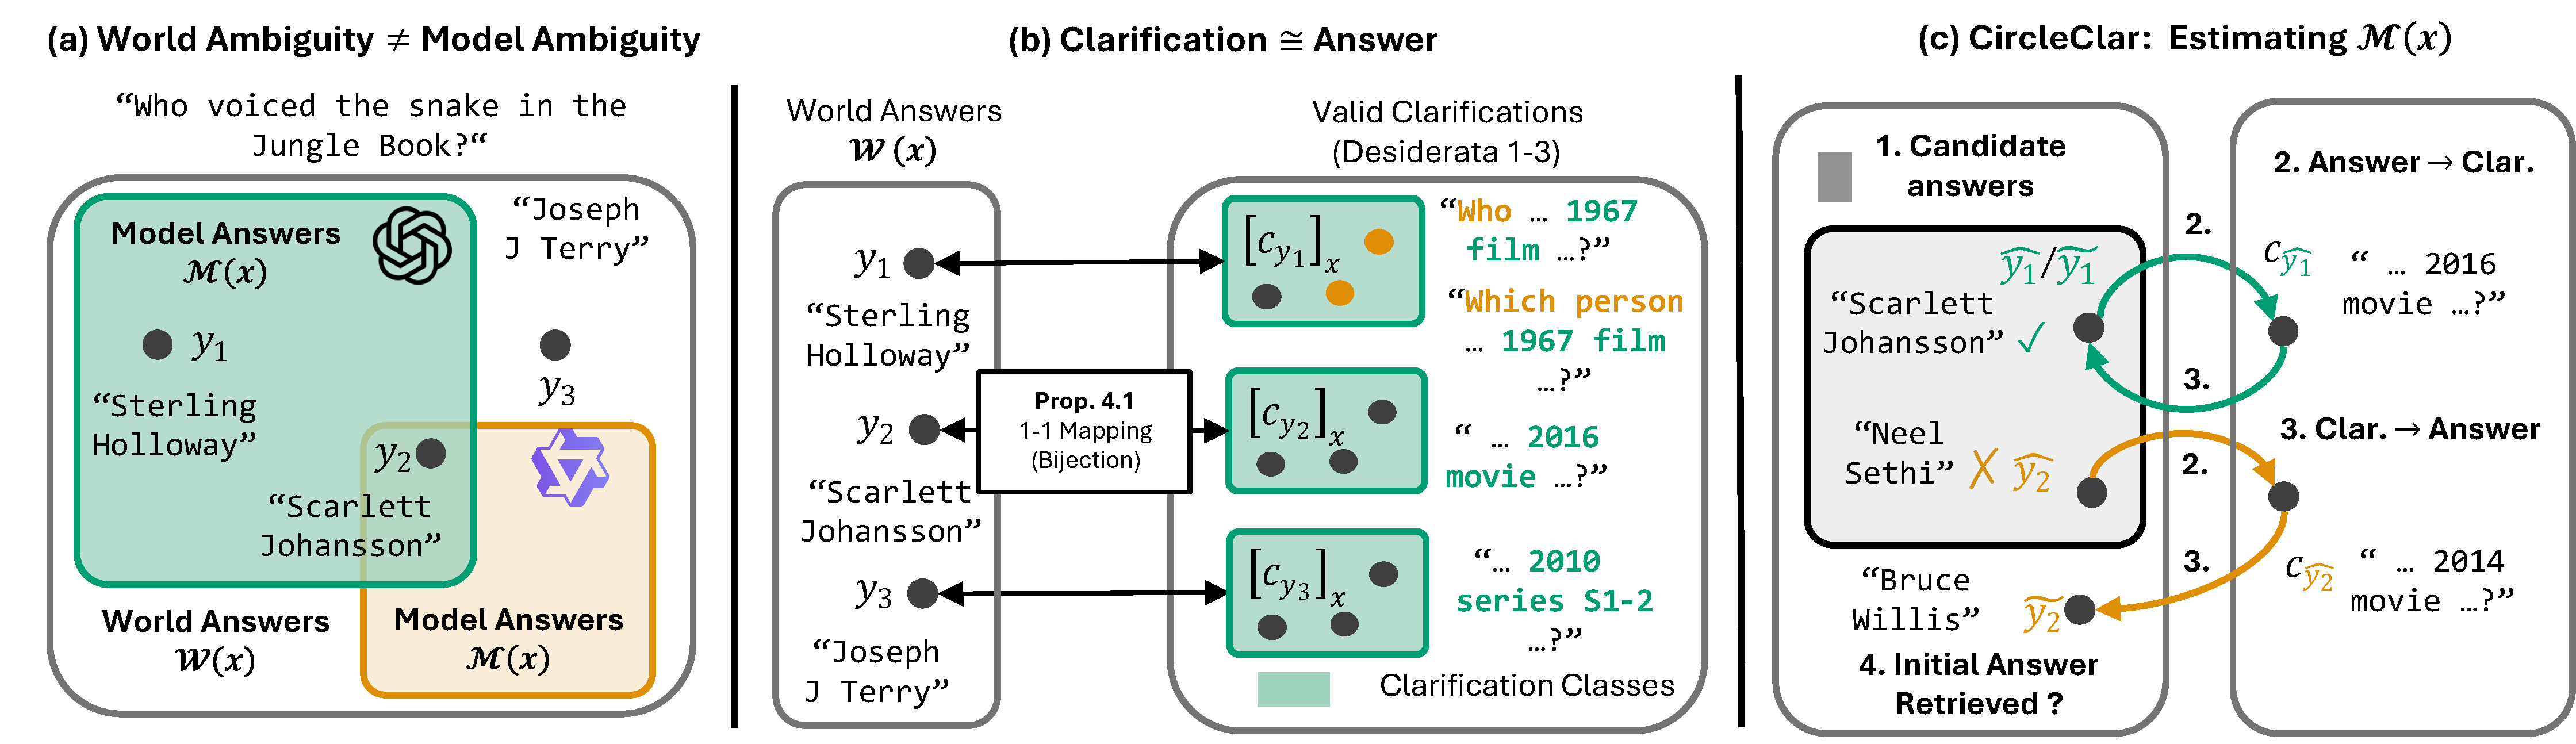
\includegraphics[width=.99\linewidth]{figures/Figure1_fixed.pdf}
    }
    \vspace{-0.25em}
    \caption{
        \textbf{Overview of our framework}: illustrated with the ambiguous question ``Who voiced the snake in \textit{The Jungle Book}?''.
        (a) The world answer support \(\mathcal{W}_T(x)\) is fixed by the input, while the model-realizable support depends on the model's knowledge.
        (b) Proposition~4.1 establishes a one-to-one correspondence between world-supported answers and clarification classes representing the same interpretations.
        (c) \circleclar{} estimates the model-realizable support by testing whether candidate answers are recovered through answer--clarification--answer cycles.
    }
    \label{fig:figure1}
    \vspace{-0.35em}
\end{figure}





\section{Related Work}
\begin{comment}
    (the roadmap. 
    start from traindition input ambiguity, NLP, dialogue, ... 
    -> modern benchmarks  ambigqa, ambient, clamner, 
    -> ) no 
    

\paragraph{Ambiguity in LLMs}
Research on underspecified requests has approaches ambiguity from two
directions. Datasets such as AmbigQA and AMBROSIA map out different meanings of a prompt by pairing its valid interpretations with rewritten questions or
executable queries \citep{min-etal-2020-ambigqa,NEURIPS2024_a4c942a8}. Other
work focuses on a more interactive setting of what the system should do next: answer immediately or ask the
user for more detail
\citep{cole-etal-2023-selectively,kuhn2023clamselectiveclarificationambiguous,zhang-choi-2025-clarify}. APA is
in spirit similar to our method because it also models perceived ambiguity
dependent on the LLMs own knowledge by using self-disambiguation as an estimate of ambiguity
\citep{kim2024aligninglanguagemodelsexplicitly}. We connect these lines of research by asking which answers to the prompt the LLM can actually produce
once each reading is made explicit. The size of this set guides whether the
model should abstain, answer, or clarify, while its members provide the content
of that response.

TODO: Add here that they look at model ambituiy\citet{kim2024aligninglanguagemodelsexplicitly} 



\paragraph{What is this section about}
\circleclar{} is closest in spirit to ICE \citep{pmlr-v235-hou24b} and CLARA \citep{rosseeuw2025clara}, which both use
model-generated clarifications to make the possible readings of an input
visible. ICE answers several clarified versions and uses the variation among
them to decompose uncertainty to assess ambiguity
\citep{pmlr-v235-hou24b}. CLARA only considers the
clarification stage and measures how many rewrites the model produces and how
different these are in meaning \citep{rosseeuw2025clara}. It deliberately avoids
answering those rewrites, making its proxy for ambiguity less tied to factual knowledge. In contrast, \circleclar{}
explicitly leverages factual knowledge in the LLM to assess model-dependent ambiguity: the estimated set of clarifications should reflect which interpretations an 
LLM can actually answer. 
Our proposed
answer--clarification--answer cycle to generate a set of valid clarifications resembles round-trip checks used in
synthetic and ambiguous QA
\citep{alberti-etal-2019-synthetic,gao-etal-2021-answering}. Returning to the
starting answer gives each cycle a semantic anchor, helping to separate a rewrite
that merely produces stable responses from one that preserves the possibility
we began with.

\end{comment}

\paragraph{Representing input ambiguity.}
\looseness=-1 A common way to study input ambiguity is to make the possible interpretations of an underspecified input explicit.
In open-domain QA, interpretations can be expressed through disambiguated questions, either provided as annotations \citep{min-etal-2020-ambigqa} or generated recursively as part of answering ambiguous questions \citep{kim-etal-2023-tree}.
In semantic parsing, where natural-language inputs are mapped to executable representations, such as SQL queries or tool calls, different interpretations can be expressed as distinct executable programs~\citep{bhaskar-etal-2023-benchmarking,NEURIPS2024_a4c942a8}, or first stated in natural language before being mapped to logical forms~\citep{saparina-lapata-2025-disambiguate}. Related work also makes alternative readings explicit as structured interpretation--answer pairs~\citep{saparina2026reasoningintentambiguousrequests}, while \citet{tomov2026illusioncertaintyuncertaintyquantification} take a distributional view, representing ambiguity through a ground-truth distribution over semantic answer classes and their relative likelihoods.
Beyond such explicit representations, \citet{pmlr-v267-kirchhof25b} takes a more general view of underspecification, describing it as uncertainty about the intended task or as missing contextual information, modeled via a latent variable model.

\iffalse
\paragraph{Clarification through interaction.}
When interaction with the user is possible, ambiguity can instead be resolved by asking for additional information that distinguishes between plausible interpretations.
Clarification requests have a long history in dialogue research~\citep{schlangen-2004-causes}.
Recent work studies how to select useful clarification questions: STaR-GATE~\citep{andukuri2024stargate} trains models to elicit user preferences that improve the eventual response, while \citet{kobalczyk2025active} use Bayesian experimental design to select clarifying questions that maximize expected information gain over compatible solutions.
Other work studies complete multi-turn clarification policies, including when and what to ask, when to stop, and how the resulting interaction affects final task performance~\citep{zhao-etal-2026-ask,ta2026turnregretregretbasedmultiturn}.
Together, these works treat clarification primarily as an interactive decision problem, focusing on what information to request and how to use the resulting user feedback.
\fi


\paragraph{Estimating input ambiguity.} 
Recent work treats input ambiguity as a quantity that can be estimated from model outputs.
ICE~\citep{pmlr-v235-hou24b} treats it as a source of aleatoric uncertainty. It generates multiple clarifications of the input, obtains predictions for each, and ensembles them to separate aleatoric uncertainty from epistemic uncertainty.
Spectral Uncertainty~\citep{epub135635} extends this approach by doing soft clustering via embeddings.
%similarly generates clarifications, but represents the resulting predictions through semantic-similarity kernels and uses von Neumann entropy to decompose uncertainty into aleatoric and epistemic components.
CLARA~\citep{rosseeuw2025clara} generates multiple clarifications and uses their semantic diversity as an ambiguity signal, while ~\citet{shi-etal-2025-ambiguity} detect ambiguity from sampled-answer distributions.
CLUES~\citep{ziletti-dambrosi-2026-disentangling} instead uses a two-stage process from interpretations to answers, separating uncertainty across interpretations from instability in their associated answers.


\paragraph{Clarifications \& input ambiguity.}
Beyond estimating ambiguity itself, other work incorporates ambiguity detection or recognition into clarification systems, benchmarks, and policies.
~\citet{lee-etal-2023-asking} formulate open-domain QA as a pipeline that detects ambiguous questions, presents candidate interpretations in a clarification question, and answers based on the user's response.
CLAM~\citep{kuhn2023clamselectiveclarificationambiguous} similarly classifies whether a question is ambiguous and selectively requests clarification before answering.
CLAMBER~\citep{zhang-etal-2024-clamber} jointly benchmarks the identification of ambiguous information needs and the generation of clarification questions.
INTENT-SIM~\citep{zhang-choi-2025-clarify} estimates entropy over simulated user intents to determine when clarification is beneficial.
ACT~\citep{chen2025learning} learns multi-turn clarification policies and evaluates implicit ambiguity recognition through models' clarify-or-answer decisions.
Zhang, Knox, and Choi~\citep{zhang2025modeling} use simulated future conversation turns to train clarify-or-answer behavior and evaluate the resulting decisions against ambiguity labels.
Su and Cardie~\citep{su2026knowingshowingllmsrecognize} further show that ambiguity recognition capability does not necessarily translate into clarification behavior: models often identify an input as ambiguous when asked explicitly, yet default to answering in ordinary QA.
Closely related to our work, BAG~\citep{baan2026clarify} uses sampled responses as a belief state to guide whether to answer, clarify, or abstain. Its BAG3 variant groups responses by meaning and proposes interpretations for each group to distinguish alternative readings from factual inconsistencies.
%gap part! 


\looseness=-1Overall, prior work studied how ambiguity can be represented, estimated, and handled through clarifications. Far less attention has been paid to how ambiguity varies with the responding model's own knowledge. APA~\citep{kim-etal-2024-aligning} recognizes this, defining perceived ambiguity as a property of a particular model and measuring it through the reduction in the model's average token entropy from the original question to a self-disambiguated version.
While conceptually sharing this perspective, our work goes further by formally distinguishing the two different types of ambiguity and defining not only a quantitative estimator but also actionable estimates of clarifications and their answers.

%asks the model to self-disambiguate the input and measures the resulting reduction in uncertainty as information gain, which is 

%then used to identify inputs perceived as ambiguous and align the model to request clarification.

%Our work shares this perspective by asking not only whether a model perceives an input as ambiguous, but furthermore which valid interpretations it can actually answer confidently. We therefore distinguish the ambiguity admitted by the input from the ambiguity realizable by a particular model; the latter depends on the model's knowledge and capabilities. This distinction is highly consequential for interaction: the same underspecified input can present different decision problems to different models, even though the set of valid interpretations itself remains unchanged.


\section{Why Input Ambiguity Should be Model Dependent}
\label{sec:motivation}

\begin{comment}
\paragraph{Setup}
LLMs implicitly define a probability distribution over arbitrary-length
strings \(s\in\mathcal{V}^{<\infty}\) from a vocabulary \(\mathcal{V}\),
which we denote by \(p(s)\). Conditioning on an input prompt
\(x\in\mathcal{V}^{<\infty}\) yields the predictive distribution
\(p(s\mid x)\). For a given task \(T\), we define \(\mathcal{Y}_T\) as the
task-relevant output space. That is, we create equivalence classes that group
together outputs \(y\) that have the same meaning for the given task.
Naturally, the model then induces a predictive distribution over this space
\(p_T(y\mid x)\). Similarly, we have an unknown true distribution
\(p_T^\star(y\mid x)\) which, by definition, is not known. 



\paragraph{World \& Model Ambiguity} When discussing an ambiguous question, one must first define its precise
meaning. We define the \emph{world outcome support} as
\[
    \mathcal{W}_T(x)
    :=
    \operatorname{supp}p_T^\star(\cdot\mid x)
    =
    \{y\in\mathcal{Y}_T:p_T^\star(y\mid x)>0\}. 
\]
Given this an ambiguous question is a question where
\(\lvert\mathcal{W}_T(x)\rvert>1\), or equivalently
\(H[p_T^\star(y\mid x)]>0\). Simply put, this is a question where there is more
than one answer in our task-relevant space. Clearly, this is a property of the
objective ground-truth mapping \(p_T^\star\) and not the model \(p_T\). The
model can produce an arbitrary distribution over answers, but we define its
set of answers, which are also in the ground truth, as the
\emph{model-realizable outcome support}:
\[
    \mathcal{M}_T(x)
    :=
    \operatorname{supp}p_T(\cdot\mid x)\cap\mathcal{W}_T(x)
    =
    \{y\in\mathcal{W}_T(x):p_T(y\mid x)>0\}.\footnote{Technically an LLM without top-p / top-k sampling assigns a nonzero probability to every sequence}
\]



\begin{wrapfigure}{r}{0.45\columnwidth}
    \centering
    \includegraphics[
        width=\linewidth
    ]{figures/model_realizable_scaling.pdf}
    \caption{
        \textbf{Model-realizable outcome spaces are model dependent.}
        Mean model-realizable outcome-space size
        $|\mathcal{M}_T(x)|$ increases with model size, but is naturally bounded by the mean world-valid outcome-space
        size, $|\mathcal{W}_T(x)|=3.85$.
    }
    \label{fig:model-realizable-space}
\end{wrapfigure}

By definition, \(\mathcal{M}_T(x)\subseteq\mathcal{W}_T(x)\), and hence
\(\lvert\mathcal{M}_T(x)\rvert\leq\lvert\mathcal{W}_T(x)\rvert\), meaning that
the model-dependent ambiguity is no larger than the world ambiguity. This
emphasizes our point that they are two possibly quite different objects. While
we can expect stronger and stronger models to capture more and more ambiguity,
with \(\lvert\mathcal{M}_T(x)\rvert\) approaching
\(\lvert\mathcal{W}_T(x)\rvert\), smaller models in particular cannot be
expected to be aware of all ambiguity. Empirical evidence for this is in
Figure~\ref{fig:model-realizable-space}. This naturally makes the goal of estimating \(\mathcal{W}_T(x)\)
with smaller models especially ineffective, \emph{as a model cannot be aware
of ambiguity it doesn't know that exists}. Rather, we argue the goal should be
to estimate \(\mathcal{M}_T(x)\), i.e., the ambiguity the model knows exists.





So how do we go about estimating this ambiguity?  
\end{comment}

%To address this gap \todo{align with contributions and related work}, we first propose 3 desiderata as required properties from clarifications. Based on these, we derive \circleclar{} as an approach that ensures our data is based on a answer--clarification--answer cycle tha ensures stability in the clarified answers..


\looseness=-1 Ambiguity is typically treated as a property of the input: a question is ambiguous when it admits multiple valid interpretations. As such, most prior work \citep{min-etal-2020-ambigqa,cole-etal-2023-selectively,liu-etal-2023-afraid,kim-etal-2023-tree,pmlr-v235-hou24b,NEURIPS2024_a4c942a8} studies ambiguity independently of the used model. Similar to \citet{kim-etal-2024-aligning}, we propose to \textit{treat ambiguity as dependent on model knowledge and, therefore, as a model-dependent property}. We formalize this distinction below and empirically show that it varies substantially across models (\Cref{fig:model-realizable-space}), motivating our model-dependent framework for characterizing ambiguity.


\paragraph{Preliminaries.}
LLMs implicitly define a probability distribution \(p(s)\) over arbitrary-length strings \(s \in \mathcal{V}^{<\infty}\) from a vocabulary \(\mathcal{V}\). Conditioned on an input \(x \in \mathcal{V}^{<\infty}\), the model induces a task-specific predictive distribution \(p_T(y \mid x)\) over answers \(y\) for a task \(T\). We analogously denote by \(p_T^\star(y \mid x)\) the corresponding unknown ground-truth distribution. Importantly, we consider answers in a task-relevant output space \(\mathcal{Y}_T\), which abstracts away distinctions that are irrelevant to the task, like surface form or syntax, by aggregating responses with similar semantic meaning into one element \cite{tomov2026taskawareness}. For question answering, for example, semantically equivalent answer strings correspond to the same element of \(\mathcal{Y}_T\); for executable outputs, such as SQL queries, syntactically different forms are treated as equivalent when they return the same requested information.



\textbf{World vs. Model Ambiguity.}
An ambiguous question \(x\) admits multiple interpretations, which may in turn lead to different correct answers. 
In the running example, the unspecified film yields Sterling Holloway or Scarlett Johansson. 
We call the set of all such answers the \emph{world answer support},
\[
    \mathcal{W}_T(x)
    :=
    \operatorname{supp} p_T^\star(\cdot \mid x)
    =
    \{y \in \mathcal{Y}_T : p_T^\star(y \mid x) > 0\},
\]
where \(p_T^\star\) denotes an oracle or ground-truth mapping.
The corresponding \emph{world ambiguity} is simply
\(|\mathcal{W}_T(x)|\), the number of correct answers admitted by the question.
In particular, \(x\) is \emph{world} ambiguous whenever there is more than one correct answer, i.e.
\(|\mathcal{W}_T(x)| > 1\).

Crucially, however, world ambiguity need not coincide with the ambiguity realized by a particular model.
Returning to our example, a model that knows both Jungle Book films can realize that the question admits at least two interpretations and associate each with its corresponding answer. In contrast, another model may only know the 2016 film---due, for instance, to differences in training data, capacity, distillation, or compression---and therefore realize only Scarlett Johansson as a valid answer.
The underlying question is equally ambiguous in both cases: its world answer support \(\mathcal{W}_T(x)\) has not changed.
What changes is which parts of this ambiguity are accessible to the model. To capture this distinction, for a model \(p_T\) we define its \emph{model-realizable answer support} as
\[
    \mathcal{M}_T(x)
    :=
    \operatorname{supp} p_T(\cdot \mid x) \cap \mathcal{W}_T(x)
    =
    \{y \in \mathcal{W}_T(x) : p_T(y \mid x) > 0\}.\footnote{Technically, an LLM without top-\(p\) or top-\(k\) sampling assigns non-zero probability to every sequence; in practice, we consider outcomes with non-negligible probability mass.}
\]
\begin{wrapfigure}{r}{0.37\columnwidth}
    \centering
    \resizebox{\linewidth}{!}{%
        %% Creator: Matplotlib, PGF backend
%%
%% To include the figure in your LaTeX document, write
%%   \input{<filename>.pgf}
%%
%% Make sure the required packages are loaded in your preamble
%%   \usepackage{pgf}
%%
%% Also ensure that all the required font packages are loaded; for instance,
%% the lmodern package is sometimes necessary when using math font.
%%   \usepackage{lmodern}
%%
%% Figures using additional raster images can only be included by \input if
%% they are in the same directory as the main LaTeX file. For loading figures
%% from other directories you can use the `import` package
%%   \usepackage{import}
%%
%% and then include the figures with
%%   \import{<path to file>}{<filename>.pgf}
%%
%% Matplotlib used the following preamble
%%   \def\mathdefault#1{#1}
%%   \everymath=\expandafter{\the\everymath\displaystyle}
%%   \IfFileExists{scrextend.sty}{
%%     \usepackage[fontsize=9.000000pt]{scrextend}
%%   }{
%%     \renewcommand{\normalsize}{\fontsize{9.000000}{10.800000}\selectfont}
%%     \normalsize
%%   }
%%   \usepackage[utf8]{inputenc}\usepackage[T1]{fontenc}\usepackage{amsmath} \usepackage{amsbsy} \newcommand*{\mat}[1]{\boldsymbol{#1}} \newcommand{\ours}{$R_{\text{Bayes}}$ {\tiny (ours)}} \newcommand{\MSP}{MSP} \newcommand{\SE}{SE} \newcommand{\KLE}{KLE} \newcommand{\COCOA}{CoCoa} \newcommand{\SAR}{SAR} \newcommand{\PTrue}{$P(\text{True})$} \renewcommand{\rmdefault}{ptm}
%%   \ifdefined\pdftexversion\else  % non-pdftex case.
%%     \usepackage{fontspec}
%%     \setmainfont{DejaVuSans.ttf}[Path=\detokenize{/nfs/homedirs/tjin/projects/llm_uncertainty/.pixi/envs/default/lib/python3.10/site-packages/matplotlib/mpl-data/fonts/ttf/}]
%%     \setsansfont{DejaVuSans.ttf}[Path=\detokenize{/nfs/homedirs/tjin/projects/llm_uncertainty/.pixi/envs/default/lib/python3.10/site-packages/matplotlib/mpl-data/fonts/ttf/}]
%%     \setmonofont{DejaVuSans.ttf}[Path=\detokenize{/nfs/homedirs/tjin/projects/llm_uncertainty/.pixi/envs/default/lib/python3.10/site-packages/matplotlib/mpl-data/fonts/ttf/}]
%%   \fi
%%   \makeatletter\@ifpackageloaded{underscore}{}{\usepackage[strings]{underscore}}\makeatother
%%
\begingroup%
\makeatletter%
\begin{pgfpicture}%
\pgfpathrectangle{\pgfpointorigin}{\pgfqpoint{2.465436in}{2.230464in}}%
\pgfusepath{use as bounding box, clip}%
\begin{pgfscope}%
\pgfsetbuttcap%
\pgfsetmiterjoin%
\definecolor{currentfill}{rgb}{1.000000,1.000000,1.000000}%
\pgfsetfillcolor{currentfill}%
\pgfsetlinewidth{0.000000pt}%
\definecolor{currentstroke}{rgb}{1.000000,1.000000,1.000000}%
\pgfsetstrokecolor{currentstroke}%
\pgfsetdash{}{0pt}%
\pgfpathmoveto{\pgfqpoint{0.000000in}{0.000000in}}%
\pgfpathlineto{\pgfqpoint{2.465436in}{0.000000in}}%
\pgfpathlineto{\pgfqpoint{2.465436in}{2.230464in}}%
\pgfpathlineto{\pgfqpoint{0.000000in}{2.230464in}}%
\pgfpathlineto{\pgfqpoint{0.000000in}{0.000000in}}%
\pgfpathclose%
\pgfusepath{fill}%
\end{pgfscope}%
\begin{pgfscope}%
\pgfsetbuttcap%
\pgfsetmiterjoin%
\definecolor{currentfill}{rgb}{1.000000,1.000000,1.000000}%
\pgfsetfillcolor{currentfill}%
\pgfsetlinewidth{0.000000pt}%
\definecolor{currentstroke}{rgb}{0.000000,0.000000,0.000000}%
\pgfsetstrokecolor{currentstroke}%
\pgfsetstrokeopacity{0.000000}%
\pgfsetdash{}{0pt}%
\pgfpathmoveto{\pgfqpoint{0.350436in}{0.872307in}}%
\pgfpathlineto{\pgfqpoint{2.455436in}{0.872307in}}%
\pgfpathlineto{\pgfqpoint{2.455436in}{2.220386in}}%
\pgfpathlineto{\pgfqpoint{0.350436in}{2.220386in}}%
\pgfpathlineto{\pgfqpoint{0.350436in}{0.872307in}}%
\pgfpathclose%
\pgfusepath{fill}%
\end{pgfscope}%
\begin{pgfscope}%
\pgfsetbuttcap%
\pgfsetroundjoin%
\definecolor{currentfill}{rgb}{0.000000,0.000000,0.000000}%
\pgfsetfillcolor{currentfill}%
\pgfsetlinewidth{0.752812pt}%
\definecolor{currentstroke}{rgb}{0.000000,0.000000,0.000000}%
\pgfsetstrokecolor{currentstroke}%
\pgfsetdash{}{0pt}%
\pgfsys@defobject{currentmarker}{\pgfqpoint{-0.041667in}{0.000000in}}{\pgfqpoint{-0.000000in}{0.000000in}}{%
\pgfpathmoveto{\pgfqpoint{-0.000000in}{0.000000in}}%
\pgfpathlineto{\pgfqpoint{-0.041667in}{0.000000in}}%
\pgfusepath{stroke,fill}%
}%
\begin{pgfscope}%
\pgfsys@transformshift{0.350436in}{0.872307in}%
\pgfsys@useobject{currentmarker}{}%
\end{pgfscope}%
\end{pgfscope}%
\begin{pgfscope}%
\definecolor{textcolor}{rgb}{0.000000,0.000000,0.000000}%
\pgfsetstrokecolor{textcolor}%
\pgfsetfillcolor{textcolor}%
\pgftext[x=0.204795in, y=0.839349in, left, base]{\color{textcolor}{\rmfamily\fontsize{7.000000}{8.400000}\selectfont\catcode`\^=\active\def^{\ifmmode\sp\else\^{}\fi}\catcode`\%=\active\def%{\%}$\mathdefault{0}$}}%
\end{pgfscope}%
\begin{pgfscope}%
\pgfpathrectangle{\pgfqpoint{0.350436in}{0.872307in}}{\pgfqpoint{2.105000in}{1.348080in}}%
\pgfusepath{clip}%
\pgfsetrectcap%
\pgfsetroundjoin%
\pgfsetlinewidth{0.501875pt}%
\definecolor{currentstroke}{rgb}{0.800000,0.800000,0.800000}%
\pgfsetstrokecolor{currentstroke}%
\pgfsetstrokeopacity{0.380000}%
\pgfsetdash{}{0pt}%
\pgfpathmoveto{\pgfqpoint{0.350436in}{1.201107in}}%
\pgfpathlineto{\pgfqpoint{2.455436in}{1.201107in}}%
\pgfusepath{stroke}%
\end{pgfscope}%
\begin{pgfscope}%
\pgfsetbuttcap%
\pgfsetroundjoin%
\definecolor{currentfill}{rgb}{0.000000,0.000000,0.000000}%
\pgfsetfillcolor{currentfill}%
\pgfsetlinewidth{0.752812pt}%
\definecolor{currentstroke}{rgb}{0.000000,0.000000,0.000000}%
\pgfsetstrokecolor{currentstroke}%
\pgfsetdash{}{0pt}%
\pgfsys@defobject{currentmarker}{\pgfqpoint{-0.041667in}{0.000000in}}{\pgfqpoint{-0.000000in}{0.000000in}}{%
\pgfpathmoveto{\pgfqpoint{-0.000000in}{0.000000in}}%
\pgfpathlineto{\pgfqpoint{-0.041667in}{0.000000in}}%
\pgfusepath{stroke,fill}%
}%
\begin{pgfscope}%
\pgfsys@transformshift{0.350436in}{1.201107in}%
\pgfsys@useobject{currentmarker}{}%
\end{pgfscope}%
\end{pgfscope}%
\begin{pgfscope}%
\definecolor{textcolor}{rgb}{0.000000,0.000000,0.000000}%
\pgfsetstrokecolor{textcolor}%
\pgfsetfillcolor{textcolor}%
\pgftext[x=0.204795in, y=1.168149in, left, base]{\color{textcolor}{\rmfamily\fontsize{7.000000}{8.400000}\selectfont\catcode`\^=\active\def^{\ifmmode\sp\else\^{}\fi}\catcode`\%=\active\def%{\%}$\mathdefault{1}$}}%
\end{pgfscope}%
\begin{pgfscope}%
\pgfpathrectangle{\pgfqpoint{0.350436in}{0.872307in}}{\pgfqpoint{2.105000in}{1.348080in}}%
\pgfusepath{clip}%
\pgfsetrectcap%
\pgfsetroundjoin%
\pgfsetlinewidth{0.501875pt}%
\definecolor{currentstroke}{rgb}{0.800000,0.800000,0.800000}%
\pgfsetstrokecolor{currentstroke}%
\pgfsetstrokeopacity{0.380000}%
\pgfsetdash{}{0pt}%
\pgfpathmoveto{\pgfqpoint{0.350436in}{1.529906in}}%
\pgfpathlineto{\pgfqpoint{2.455436in}{1.529906in}}%
\pgfusepath{stroke}%
\end{pgfscope}%
\begin{pgfscope}%
\pgfsetbuttcap%
\pgfsetroundjoin%
\definecolor{currentfill}{rgb}{0.000000,0.000000,0.000000}%
\pgfsetfillcolor{currentfill}%
\pgfsetlinewidth{0.752812pt}%
\definecolor{currentstroke}{rgb}{0.000000,0.000000,0.000000}%
\pgfsetstrokecolor{currentstroke}%
\pgfsetdash{}{0pt}%
\pgfsys@defobject{currentmarker}{\pgfqpoint{-0.041667in}{0.000000in}}{\pgfqpoint{-0.000000in}{0.000000in}}{%
\pgfpathmoveto{\pgfqpoint{-0.000000in}{0.000000in}}%
\pgfpathlineto{\pgfqpoint{-0.041667in}{0.000000in}}%
\pgfusepath{stroke,fill}%
}%
\begin{pgfscope}%
\pgfsys@transformshift{0.350436in}{1.529906in}%
\pgfsys@useobject{currentmarker}{}%
\end{pgfscope}%
\end{pgfscope}%
\begin{pgfscope}%
\definecolor{textcolor}{rgb}{0.000000,0.000000,0.000000}%
\pgfsetstrokecolor{textcolor}%
\pgfsetfillcolor{textcolor}%
\pgftext[x=0.204795in, y=1.496949in, left, base]{\color{textcolor}{\rmfamily\fontsize{7.000000}{8.400000}\selectfont\catcode`\^=\active\def^{\ifmmode\sp\else\^{}\fi}\catcode`\%=\active\def%{\%}$\mathdefault{2}$}}%
\end{pgfscope}%
\begin{pgfscope}%
\pgfpathrectangle{\pgfqpoint{0.350436in}{0.872307in}}{\pgfqpoint{2.105000in}{1.348080in}}%
\pgfusepath{clip}%
\pgfsetrectcap%
\pgfsetroundjoin%
\pgfsetlinewidth{0.501875pt}%
\definecolor{currentstroke}{rgb}{0.800000,0.800000,0.800000}%
\pgfsetstrokecolor{currentstroke}%
\pgfsetstrokeopacity{0.380000}%
\pgfsetdash{}{0pt}%
\pgfpathmoveto{\pgfqpoint{0.350436in}{1.858706in}}%
\pgfpathlineto{\pgfqpoint{2.455436in}{1.858706in}}%
\pgfusepath{stroke}%
\end{pgfscope}%
\begin{pgfscope}%
\pgfsetbuttcap%
\pgfsetroundjoin%
\definecolor{currentfill}{rgb}{0.000000,0.000000,0.000000}%
\pgfsetfillcolor{currentfill}%
\pgfsetlinewidth{0.752812pt}%
\definecolor{currentstroke}{rgb}{0.000000,0.000000,0.000000}%
\pgfsetstrokecolor{currentstroke}%
\pgfsetdash{}{0pt}%
\pgfsys@defobject{currentmarker}{\pgfqpoint{-0.041667in}{0.000000in}}{\pgfqpoint{-0.000000in}{0.000000in}}{%
\pgfpathmoveto{\pgfqpoint{-0.000000in}{0.000000in}}%
\pgfpathlineto{\pgfqpoint{-0.041667in}{0.000000in}}%
\pgfusepath{stroke,fill}%
}%
\begin{pgfscope}%
\pgfsys@transformshift{0.350436in}{1.858706in}%
\pgfsys@useobject{currentmarker}{}%
\end{pgfscope}%
\end{pgfscope}%
\begin{pgfscope}%
\definecolor{textcolor}{rgb}{0.000000,0.000000,0.000000}%
\pgfsetstrokecolor{textcolor}%
\pgfsetfillcolor{textcolor}%
\pgftext[x=0.204795in, y=1.825749in, left, base]{\color{textcolor}{\rmfamily\fontsize{7.000000}{8.400000}\selectfont\catcode`\^=\active\def^{\ifmmode\sp\else\^{}\fi}\catcode`\%=\active\def%{\%}$\mathdefault{3}$}}%
\end{pgfscope}%
\begin{pgfscope}%
\pgfsetbuttcap%
\pgfsetroundjoin%
\definecolor{currentfill}{rgb}{0.000000,0.000000,0.000000}%
\pgfsetfillcolor{currentfill}%
\pgfsetlinewidth{0.752812pt}%
\definecolor{currentstroke}{rgb}{0.000000,0.000000,0.000000}%
\pgfsetstrokecolor{currentstroke}%
\pgfsetdash{}{0pt}%
\pgfsys@defobject{currentmarker}{\pgfqpoint{-0.041667in}{0.000000in}}{\pgfqpoint{-0.000000in}{0.000000in}}{%
\pgfpathmoveto{\pgfqpoint{-0.000000in}{0.000000in}}%
\pgfpathlineto{\pgfqpoint{-0.041667in}{0.000000in}}%
\pgfusepath{stroke,fill}%
}%
\begin{pgfscope}%
\pgfsys@transformshift{0.350436in}{2.187506in}%
\pgfsys@useobject{currentmarker}{}%
\end{pgfscope}%
\end{pgfscope}%
\begin{pgfscope}%
\definecolor{textcolor}{rgb}{0.000000,0.000000,0.000000}%
\pgfsetstrokecolor{textcolor}%
\pgfsetfillcolor{textcolor}%
\pgftext[x=0.204795in, y=2.154549in, left, base]{\color{textcolor}{\rmfamily\fontsize{7.000000}{8.400000}\selectfont\catcode`\^=\active\def^{\ifmmode\sp\else\^{}\fi}\catcode`\%=\active\def%{\%}$\mathdefault{4}$}}%
\end{pgfscope}%
\begin{pgfscope}%
\definecolor{textcolor}{rgb}{0.000000,0.000000,0.000000}%
\pgfsetstrokecolor{textcolor}%
\pgfsetfillcolor{textcolor}%
\pgftext[x=0.163128in,y=1.546346in,,bottom,rotate=90.000000]{\color{textcolor}{\rmfamily\fontsize{7.000000}{8.400000}\selectfont\catcode`\^=\active\def^{\ifmmode\sp\else\^{}\fi}\catcode`\%=\active\def%{\%}Mean $\lvert\mathcal{M}_T(x)\rvert$}}%
\end{pgfscope}%
\begin{pgfscope}%
\pgfpathrectangle{\pgfqpoint{0.350436in}{0.872307in}}{\pgfqpoint{2.105000in}{1.348080in}}%
\pgfusepath{clip}%
\pgfsetbuttcap%
\pgfsetroundjoin%
\pgfsetlinewidth{0.803000pt}%
\definecolor{currentstroke}{rgb}{0.372549,0.372549,0.372549}%
\pgfsetstrokecolor{currentstroke}%
\pgfsetdash{{2.400000pt}{1.600000pt}}{0.000000pt}%
\pgfpathmoveto{\pgfqpoint{0.350436in}{2.076701in}}%
\pgfpathlineto{\pgfqpoint{2.455436in}{2.076701in}}%
\pgfusepath{stroke}%
\end{pgfscope}%
\begin{pgfscope}%
\pgfpathrectangle{\pgfqpoint{0.350436in}{0.872307in}}{\pgfqpoint{2.105000in}{1.348080in}}%
\pgfusepath{clip}%
\pgfsetbuttcap%
\pgfsetmiterjoin%
\definecolor{currentfill}{rgb}{0.007843,0.619608,0.450980}%
\pgfsetfillcolor{currentfill}%
\pgfsetfillopacity{0.800000}%
\pgfsetlinewidth{0.000000pt}%
\definecolor{currentstroke}{rgb}{0.000000,0.000000,0.000000}%
\pgfsetstrokecolor{currentstroke}%
\pgfsetstrokeopacity{0.800000}%
\pgfsetdash{}{0pt}%
\pgfpathmoveto{\pgfqpoint{0.633403in}{0.872307in}}%
\pgfpathlineto{\pgfqpoint{0.826649in}{0.872307in}}%
\pgfpathlineto{\pgfqpoint{0.826649in}{1.011718in}}%
\pgfpathlineto{\pgfqpoint{0.633403in}{1.011718in}}%
\pgfpathlineto{\pgfqpoint{0.633403in}{0.872307in}}%
\pgfpathclose%
\pgfusepath{fill}%
\end{pgfscope}%
\begin{pgfscope}%
\pgfpathrectangle{\pgfqpoint{0.350436in}{0.872307in}}{\pgfqpoint{2.105000in}{1.348080in}}%
\pgfusepath{clip}%
\pgfsetbuttcap%
\pgfsetmiterjoin%
\definecolor{currentfill}{rgb}{0.007843,0.619608,0.450980}%
\pgfsetfillcolor{currentfill}%
\pgfsetfillopacity{0.800000}%
\pgfsetlinewidth{0.000000pt}%
\definecolor{currentstroke}{rgb}{0.000000,0.000000,0.000000}%
\pgfsetstrokecolor{currentstroke}%
\pgfsetstrokeopacity{0.800000}%
\pgfsetdash{}{0pt}%
\pgfpathmoveto{\pgfqpoint{1.012993in}{0.872307in}}%
\pgfpathlineto{\pgfqpoint{1.206239in}{0.872307in}}%
\pgfpathlineto{\pgfqpoint{1.206239in}{1.145211in}}%
\pgfpathlineto{\pgfqpoint{1.012993in}{1.145211in}}%
\pgfpathlineto{\pgfqpoint{1.012993in}{0.872307in}}%
\pgfpathclose%
\pgfusepath{fill}%
\end{pgfscope}%
\begin{pgfscope}%
\pgfpathrectangle{\pgfqpoint{0.350436in}{0.872307in}}{\pgfqpoint{2.105000in}{1.348080in}}%
\pgfusepath{clip}%
\pgfsetbuttcap%
\pgfsetmiterjoin%
\definecolor{currentfill}{rgb}{0.870588,0.560784,0.019608}%
\pgfsetfillcolor{currentfill}%
\pgfsetfillopacity{0.800000}%
\pgfsetlinewidth{0.000000pt}%
\definecolor{currentstroke}{rgb}{0.000000,0.000000,0.000000}%
\pgfsetstrokecolor{currentstroke}%
\pgfsetstrokeopacity{0.800000}%
\pgfsetdash{}{0pt}%
\pgfpathmoveto{\pgfqpoint{1.599632in}{0.872307in}}%
\pgfpathlineto{\pgfqpoint{1.792878in}{0.872307in}}%
\pgfpathlineto{\pgfqpoint{1.792878in}{1.284622in}}%
\pgfpathlineto{\pgfqpoint{1.599632in}{1.284622in}}%
\pgfpathlineto{\pgfqpoint{1.599632in}{0.872307in}}%
\pgfpathclose%
\pgfusepath{fill}%
\end{pgfscope}%
\begin{pgfscope}%
\pgfpathrectangle{\pgfqpoint{0.350436in}{0.872307in}}{\pgfqpoint{2.105000in}{1.348080in}}%
\pgfusepath{clip}%
\pgfsetbuttcap%
\pgfsetmiterjoin%
\definecolor{currentfill}{rgb}{0.870588,0.560784,0.019608}%
\pgfsetfillcolor{currentfill}%
\pgfsetfillopacity{0.800000}%
\pgfsetlinewidth{0.000000pt}%
\definecolor{currentstroke}{rgb}{0.000000,0.000000,0.000000}%
\pgfsetstrokecolor{currentstroke}%
\pgfsetstrokeopacity{0.800000}%
\pgfsetdash{}{0pt}%
\pgfpathmoveto{\pgfqpoint{1.979223in}{0.872307in}}%
\pgfpathlineto{\pgfqpoint{2.172468in}{0.872307in}}%
\pgfpathlineto{\pgfqpoint{2.172468in}{1.499328in}}%
\pgfpathlineto{\pgfqpoint{1.979223in}{1.499328in}}%
\pgfpathlineto{\pgfqpoint{1.979223in}{0.872307in}}%
\pgfpathclose%
\pgfusepath{fill}%
\end{pgfscope}%
\begin{pgfscope}%
\pgfsetrectcap%
\pgfsetmiterjoin%
\pgfsetlinewidth{0.752812pt}%
\definecolor{currentstroke}{rgb}{0.700000,0.700000,0.700000}%
\pgfsetstrokecolor{currentstroke}%
\pgfsetdash{}{0pt}%
\pgfpathmoveto{\pgfqpoint{0.350436in}{0.872307in}}%
\pgfpathlineto{\pgfqpoint{0.350436in}{2.220386in}}%
\pgfusepath{stroke}%
\end{pgfscope}%
\begin{pgfscope}%
\pgfsetrectcap%
\pgfsetmiterjoin%
\pgfsetlinewidth{0.752812pt}%
\definecolor{currentstroke}{rgb}{0.700000,0.700000,0.700000}%
\pgfsetstrokecolor{currentstroke}%
\pgfsetdash{}{0pt}%
\pgfpathmoveto{\pgfqpoint{0.350436in}{0.872307in}}%
\pgfpathlineto{\pgfqpoint{2.455436in}{0.872307in}}%
\pgfusepath{stroke}%
\end{pgfscope}%
\begin{pgfscope}%
\pgfsetbuttcap%
\pgfsetmiterjoin%
\definecolor{currentfill}{rgb}{1.000000,1.000000,1.000000}%
\pgfsetfillcolor{currentfill}%
\pgfsetlinewidth{0.000000pt}%
\definecolor{currentstroke}{rgb}{0.000000,0.000000,0.000000}%
\pgfsetstrokecolor{currentstroke}%
\pgfsetstrokeopacity{0.000000}%
\pgfsetdash{}{0pt}%
\pgfpathmoveto{\pgfqpoint{1.539332in}{1.948661in}}%
\pgfpathlineto{\pgfqpoint{2.397536in}{1.948661in}}%
\pgfpathlineto{\pgfqpoint{2.397536in}{2.042495in}}%
\pgfpathlineto{\pgfqpoint{1.539332in}{2.042495in}}%
\pgfpathlineto{\pgfqpoint{1.539332in}{1.948661in}}%
\pgfpathclose%
\pgfusepath{fill}%
\end{pgfscope}%
\begin{pgfscope}%
\definecolor{textcolor}{rgb}{0.501961,0.501961,0.501961}%
\pgfsetstrokecolor{textcolor}%
\pgfsetfillcolor{textcolor}%
\pgftext[x=2.392286in,y=2.037245in,right,top]{\color{textcolor}{\rmfamily\fontsize{6.300000}{7.560000}\selectfont\catcode`\^=\active\def^{\ifmmode\sp\else\^{}\fi}\catcode`\%=\active\def%{\%}Mean $\lvert\mathcal{W}_T(x)\rvert$ = 3.66}}%
\end{pgfscope}%
\begin{pgfscope}%
\pgfpathrectangle{\pgfqpoint{0.350436in}{0.872307in}}{\pgfqpoint{2.105000in}{1.348080in}}%
\pgfusepath{clip}%
\pgfsetbuttcap%
\pgfsetroundjoin%
\pgfsetlinewidth{0.903375pt}%
\definecolor{currentstroke}{rgb}{0.247059,0.247059,0.247059}%
\pgfsetstrokecolor{currentstroke}%
\pgfsetdash{}{0pt}%
\pgfpathmoveto{\pgfqpoint{0.730026in}{0.996593in}}%
\pgfpathlineto{\pgfqpoint{0.730026in}{1.027171in}}%
\pgfusepath{stroke}%
\end{pgfscope}%
\begin{pgfscope}%
\pgfpathrectangle{\pgfqpoint{0.350436in}{0.872307in}}{\pgfqpoint{2.105000in}{1.348080in}}%
\pgfusepath{clip}%
\pgfsetbuttcap%
\pgfsetroundjoin%
\pgfsetlinewidth{0.903375pt}%
\definecolor{currentstroke}{rgb}{0.247059,0.247059,0.247059}%
\pgfsetstrokecolor{currentstroke}%
\pgfsetdash{}{0pt}%
\pgfpathmoveto{\pgfqpoint{1.109616in}{1.124825in}}%
\pgfpathlineto{\pgfqpoint{1.109616in}{1.165925in}}%
\pgfusepath{stroke}%
\end{pgfscope}%
\begin{pgfscope}%
\pgfpathrectangle{\pgfqpoint{0.350436in}{0.872307in}}{\pgfqpoint{2.105000in}{1.348080in}}%
\pgfusepath{clip}%
\pgfsetbuttcap%
\pgfsetroundjoin%
\definecolor{currentfill}{rgb}{0.121569,0.466667,0.705882}%
\pgfsetfillcolor{currentfill}%
\pgfsetlinewidth{0.903375pt}%
\definecolor{currentstroke}{rgb}{0.247059,0.247059,0.247059}%
\pgfsetstrokecolor{currentstroke}%
\pgfsetdash{}{0pt}%
\pgfsys@defobject{currentmarker}{\pgfqpoint{-0.027778in}{-0.000000in}}{\pgfqpoint{0.027778in}{0.000000in}}{%
\pgfpathmoveto{\pgfqpoint{0.027778in}{-0.000000in}}%
\pgfpathlineto{\pgfqpoint{-0.027778in}{0.000000in}}%
\pgfusepath{stroke,fill}%
}%
\begin{pgfscope}%
\pgfsys@transformshift{0.730026in}{0.996593in}%
\pgfsys@useobject{currentmarker}{}%
\end{pgfscope}%
\begin{pgfscope}%
\pgfsys@transformshift{1.109616in}{1.124825in}%
\pgfsys@useobject{currentmarker}{}%
\end{pgfscope}%
\end{pgfscope}%
\begin{pgfscope}%
\pgfpathrectangle{\pgfqpoint{0.350436in}{0.872307in}}{\pgfqpoint{2.105000in}{1.348080in}}%
\pgfusepath{clip}%
\pgfsetbuttcap%
\pgfsetroundjoin%
\definecolor{currentfill}{rgb}{0.121569,0.466667,0.705882}%
\pgfsetfillcolor{currentfill}%
\pgfsetlinewidth{0.903375pt}%
\definecolor{currentstroke}{rgb}{0.247059,0.247059,0.247059}%
\pgfsetstrokecolor{currentstroke}%
\pgfsetdash{}{0pt}%
\pgfsys@defobject{currentmarker}{\pgfqpoint{-0.027778in}{-0.000000in}}{\pgfqpoint{0.027778in}{0.000000in}}{%
\pgfpathmoveto{\pgfqpoint{0.027778in}{-0.000000in}}%
\pgfpathlineto{\pgfqpoint{-0.027778in}{0.000000in}}%
\pgfusepath{stroke,fill}%
}%
\begin{pgfscope}%
\pgfsys@transformshift{0.730026in}{1.027171in}%
\pgfsys@useobject{currentmarker}{}%
\end{pgfscope}%
\begin{pgfscope}%
\pgfsys@transformshift{1.109616in}{1.165925in}%
\pgfsys@useobject{currentmarker}{}%
\end{pgfscope}%
\end{pgfscope}%
\begin{pgfscope}%
\pgfpathrectangle{\pgfqpoint{0.350436in}{0.872307in}}{\pgfqpoint{2.105000in}{1.348080in}}%
\pgfusepath{clip}%
\pgfsetbuttcap%
\pgfsetroundjoin%
\pgfsetlinewidth{0.903375pt}%
\definecolor{currentstroke}{rgb}{0.247059,0.247059,0.247059}%
\pgfsetstrokecolor{currentstroke}%
\pgfsetdash{}{0pt}%
\pgfpathmoveto{\pgfqpoint{1.696255in}{1.260290in}}%
\pgfpathlineto{\pgfqpoint{1.696255in}{1.309282in}}%
\pgfusepath{stroke}%
\end{pgfscope}%
\begin{pgfscope}%
\pgfpathrectangle{\pgfqpoint{0.350436in}{0.872307in}}{\pgfqpoint{2.105000in}{1.348080in}}%
\pgfusepath{clip}%
\pgfsetbuttcap%
\pgfsetroundjoin%
\pgfsetlinewidth{0.903375pt}%
\definecolor{currentstroke}{rgb}{0.247059,0.247059,0.247059}%
\pgfsetstrokecolor{currentstroke}%
\pgfsetdash{}{0pt}%
\pgfpathmoveto{\pgfqpoint{2.075846in}{1.471051in}}%
\pgfpathlineto{\pgfqpoint{2.075846in}{1.527605in}}%
\pgfusepath{stroke}%
\end{pgfscope}%
\begin{pgfscope}%
\pgfpathrectangle{\pgfqpoint{0.350436in}{0.872307in}}{\pgfqpoint{2.105000in}{1.348080in}}%
\pgfusepath{clip}%
\pgfsetbuttcap%
\pgfsetroundjoin%
\definecolor{currentfill}{rgb}{0.121569,0.466667,0.705882}%
\pgfsetfillcolor{currentfill}%
\pgfsetlinewidth{0.903375pt}%
\definecolor{currentstroke}{rgb}{0.247059,0.247059,0.247059}%
\pgfsetstrokecolor{currentstroke}%
\pgfsetdash{}{0pt}%
\pgfsys@defobject{currentmarker}{\pgfqpoint{-0.027778in}{-0.000000in}}{\pgfqpoint{0.027778in}{0.000000in}}{%
\pgfpathmoveto{\pgfqpoint{0.027778in}{-0.000000in}}%
\pgfpathlineto{\pgfqpoint{-0.027778in}{0.000000in}}%
\pgfusepath{stroke,fill}%
}%
\begin{pgfscope}%
\pgfsys@transformshift{1.696255in}{1.260290in}%
\pgfsys@useobject{currentmarker}{}%
\end{pgfscope}%
\begin{pgfscope}%
\pgfsys@transformshift{2.075846in}{1.471051in}%
\pgfsys@useobject{currentmarker}{}%
\end{pgfscope}%
\end{pgfscope}%
\begin{pgfscope}%
\pgfpathrectangle{\pgfqpoint{0.350436in}{0.872307in}}{\pgfqpoint{2.105000in}{1.348080in}}%
\pgfusepath{clip}%
\pgfsetbuttcap%
\pgfsetroundjoin%
\definecolor{currentfill}{rgb}{0.121569,0.466667,0.705882}%
\pgfsetfillcolor{currentfill}%
\pgfsetlinewidth{0.903375pt}%
\definecolor{currentstroke}{rgb}{0.247059,0.247059,0.247059}%
\pgfsetstrokecolor{currentstroke}%
\pgfsetdash{}{0pt}%
\pgfsys@defobject{currentmarker}{\pgfqpoint{-0.027778in}{-0.000000in}}{\pgfqpoint{0.027778in}{0.000000in}}{%
\pgfpathmoveto{\pgfqpoint{0.027778in}{-0.000000in}}%
\pgfpathlineto{\pgfqpoint{-0.027778in}{0.000000in}}%
\pgfusepath{stroke,fill}%
}%
\begin{pgfscope}%
\pgfsys@transformshift{1.696255in}{1.309282in}%
\pgfsys@useobject{currentmarker}{}%
\end{pgfscope}%
\begin{pgfscope}%
\pgfsys@transformshift{2.075846in}{1.527605in}%
\pgfsys@useobject{currentmarker}{}%
\end{pgfscope}%
\end{pgfscope}%
\begin{pgfscope}%
\pgfsetbuttcap%
\pgfsetmiterjoin%
\definecolor{currentfill}{rgb}{1.000000,1.000000,1.000000}%
\pgfsetfillcolor{currentfill}%
\pgfsetlinewidth{0.000000pt}%
\definecolor{currentstroke}{rgb}{0.000000,0.000000,0.000000}%
\pgfsetstrokecolor{currentstroke}%
\pgfsetstrokeopacity{0.000000}%
\pgfsetdash{}{0pt}%
\pgfpathmoveto{\pgfqpoint{0.350436in}{0.333075in}}%
\pgfpathlineto{\pgfqpoint{2.455436in}{0.333075in}}%
\pgfpathlineto{\pgfqpoint{2.455436in}{0.782435in}}%
\pgfpathlineto{\pgfqpoint{0.350436in}{0.782435in}}%
\pgfpathlineto{\pgfqpoint{0.350436in}{0.333075in}}%
\pgfpathclose%
\pgfusepath{fill}%
\end{pgfscope}%
\begin{pgfscope}%
\pgfpathrectangle{\pgfqpoint{0.350436in}{0.333075in}}{\pgfqpoint{2.105000in}{0.449360in}}%
\pgfusepath{clip}%
\pgfsetrectcap%
\pgfsetroundjoin%
\pgfsetlinewidth{0.501875pt}%
\definecolor{currentstroke}{rgb}{0.901961,0.901961,0.901961}%
\pgfsetstrokecolor{currentstroke}%
\pgfsetdash{}{0pt}%
\pgfpathmoveto{\pgfqpoint{0.350436in}{0.565002in}}%
\pgfpathlineto{\pgfqpoint{2.455436in}{0.565002in}}%
\pgfusepath{stroke}%
\end{pgfscope}%
\begin{pgfscope}%
\pgfsetbuttcap%
\pgfsetroundjoin%
\definecolor{currentfill}{rgb}{0.000000,0.000000,0.000000}%
\pgfsetfillcolor{currentfill}%
\pgfsetlinewidth{0.752812pt}%
\definecolor{currentstroke}{rgb}{0.000000,0.000000,0.000000}%
\pgfsetstrokecolor{currentstroke}%
\pgfsetdash{}{0pt}%
\pgfsys@defobject{currentmarker}{\pgfqpoint{0.000000in}{-0.041667in}}{\pgfqpoint{0.000000in}{0.000000in}}{%
\pgfpathmoveto{\pgfqpoint{0.000000in}{0.000000in}}%
\pgfpathlineto{\pgfqpoint{0.000000in}{-0.041667in}}%
\pgfusepath{stroke,fill}%
}%
\begin{pgfscope}%
\pgfsys@transformshift{0.730026in}{0.333075in}%
\pgfsys@useobject{currentmarker}{}%
\end{pgfscope}%
\end{pgfscope}%
\begin{pgfscope}%
\definecolor{textcolor}{rgb}{0.000000,0.000000,0.000000}%
\pgfsetstrokecolor{textcolor}%
\pgfsetfillcolor{textcolor}%
\pgftext[x=0.730026in,y=0.242797in,,top]{\color{textcolor}{\rmfamily\fontsize{7.000000}{8.400000}\selectfont\catcode`\^=\active\def^{\ifmmode\sp\else\^{}\fi}\catcode`\%=\active\def%{\%}4B}}%
\end{pgfscope}%
\begin{pgfscope}%
\pgfsetbuttcap%
\pgfsetroundjoin%
\definecolor{currentfill}{rgb}{0.000000,0.000000,0.000000}%
\pgfsetfillcolor{currentfill}%
\pgfsetlinewidth{0.752812pt}%
\definecolor{currentstroke}{rgb}{0.000000,0.000000,0.000000}%
\pgfsetstrokecolor{currentstroke}%
\pgfsetdash{}{0pt}%
\pgfsys@defobject{currentmarker}{\pgfqpoint{0.000000in}{-0.041667in}}{\pgfqpoint{0.000000in}{0.000000in}}{%
\pgfpathmoveto{\pgfqpoint{0.000000in}{0.000000in}}%
\pgfpathlineto{\pgfqpoint{0.000000in}{-0.041667in}}%
\pgfusepath{stroke,fill}%
}%
\begin{pgfscope}%
\pgfsys@transformshift{1.109616in}{0.333075in}%
\pgfsys@useobject{currentmarker}{}%
\end{pgfscope}%
\end{pgfscope}%
\begin{pgfscope}%
\definecolor{textcolor}{rgb}{0.000000,0.000000,0.000000}%
\pgfsetstrokecolor{textcolor}%
\pgfsetfillcolor{textcolor}%
\pgftext[x=1.109616in,y=0.242797in,,top]{\color{textcolor}{\rmfamily\fontsize{7.000000}{8.400000}\selectfont\catcode`\^=\active\def^{\ifmmode\sp\else\^{}\fi}\catcode`\%=\active\def%{\%}30B-A3B}}%
\end{pgfscope}%
\begin{pgfscope}%
\pgfsetbuttcap%
\pgfsetroundjoin%
\definecolor{currentfill}{rgb}{0.000000,0.000000,0.000000}%
\pgfsetfillcolor{currentfill}%
\pgfsetlinewidth{0.752812pt}%
\definecolor{currentstroke}{rgb}{0.000000,0.000000,0.000000}%
\pgfsetstrokecolor{currentstroke}%
\pgfsetdash{}{0pt}%
\pgfsys@defobject{currentmarker}{\pgfqpoint{0.000000in}{-0.041667in}}{\pgfqpoint{0.000000in}{0.000000in}}{%
\pgfpathmoveto{\pgfqpoint{0.000000in}{0.000000in}}%
\pgfpathlineto{\pgfqpoint{0.000000in}{-0.041667in}}%
\pgfusepath{stroke,fill}%
}%
\begin{pgfscope}%
\pgfsys@transformshift{1.696255in}{0.333075in}%
\pgfsys@useobject{currentmarker}{}%
\end{pgfscope}%
\end{pgfscope}%
\begin{pgfscope}%
\definecolor{textcolor}{rgb}{0.000000,0.000000,0.000000}%
\pgfsetstrokecolor{textcolor}%
\pgfsetfillcolor{textcolor}%
\pgftext[x=1.696255in,y=0.242797in,,top]{\color{textcolor}{\rmfamily\fontsize{7.000000}{8.400000}\selectfont\catcode`\^=\active\def^{\ifmmode\sp\else\^{}\fi}\catcode`\%=\active\def%{\%}5.4-mini}}%
\end{pgfscope}%
\begin{pgfscope}%
\pgfsetbuttcap%
\pgfsetroundjoin%
\definecolor{currentfill}{rgb}{0.000000,0.000000,0.000000}%
\pgfsetfillcolor{currentfill}%
\pgfsetlinewidth{0.752812pt}%
\definecolor{currentstroke}{rgb}{0.000000,0.000000,0.000000}%
\pgfsetstrokecolor{currentstroke}%
\pgfsetdash{}{0pt}%
\pgfsys@defobject{currentmarker}{\pgfqpoint{0.000000in}{-0.041667in}}{\pgfqpoint{0.000000in}{0.000000in}}{%
\pgfpathmoveto{\pgfqpoint{0.000000in}{0.000000in}}%
\pgfpathlineto{\pgfqpoint{0.000000in}{-0.041667in}}%
\pgfusepath{stroke,fill}%
}%
\begin{pgfscope}%
\pgfsys@transformshift{2.075846in}{0.333075in}%
\pgfsys@useobject{currentmarker}{}%
\end{pgfscope}%
\end{pgfscope}%
\begin{pgfscope}%
\definecolor{textcolor}{rgb}{0.000000,0.000000,0.000000}%
\pgfsetstrokecolor{textcolor}%
\pgfsetfillcolor{textcolor}%
\pgftext[x=2.075846in,y=0.242797in,,top]{\color{textcolor}{\rmfamily\fontsize{7.000000}{8.400000}\selectfont\catcode`\^=\active\def^{\ifmmode\sp\else\^{}\fi}\catcode`\%=\active\def%{\%}5.5}}%
\end{pgfscope}%
\begin{pgfscope}%
\pgfsetbuttcap%
\pgfsetroundjoin%
\definecolor{currentfill}{rgb}{0.000000,0.000000,0.000000}%
\pgfsetfillcolor{currentfill}%
\pgfsetlinewidth{0.752812pt}%
\definecolor{currentstroke}{rgb}{0.000000,0.000000,0.000000}%
\pgfsetstrokecolor{currentstroke}%
\pgfsetdash{}{0pt}%
\pgfsys@defobject{currentmarker}{\pgfqpoint{-0.041667in}{0.000000in}}{\pgfqpoint{-0.000000in}{0.000000in}}{%
\pgfpathmoveto{\pgfqpoint{-0.000000in}{0.000000in}}%
\pgfpathlineto{\pgfqpoint{-0.041667in}{0.000000in}}%
\pgfusepath{stroke,fill}%
}%
\begin{pgfscope}%
\pgfsys@transformshift{0.350436in}{0.347570in}%
\pgfsys@useobject{currentmarker}{}%
\end{pgfscope}%
\end{pgfscope}%
\begin{pgfscope}%
\definecolor{textcolor}{rgb}{0.000000,0.000000,0.000000}%
\pgfsetstrokecolor{textcolor}%
\pgfsetfillcolor{textcolor}%
\pgftext[x=0.138630in, y=0.314612in, left, base]{\color{textcolor}{\rmfamily\fontsize{7.000000}{8.400000}\selectfont\catcode`\^=\active\def^{\ifmmode\sp\else\^{}\fi}\catcode`\%=\active\def%{\%}0.0}}%
\end{pgfscope}%
\begin{pgfscope}%
\pgfsetbuttcap%
\pgfsetroundjoin%
\definecolor{currentfill}{rgb}{0.000000,0.000000,0.000000}%
\pgfsetfillcolor{currentfill}%
\pgfsetlinewidth{0.752812pt}%
\definecolor{currentstroke}{rgb}{0.000000,0.000000,0.000000}%
\pgfsetstrokecolor{currentstroke}%
\pgfsetdash{}{0pt}%
\pgfsys@defobject{currentmarker}{\pgfqpoint{-0.041667in}{0.000000in}}{\pgfqpoint{-0.000000in}{0.000000in}}{%
\pgfpathmoveto{\pgfqpoint{-0.000000in}{0.000000in}}%
\pgfpathlineto{\pgfqpoint{-0.041667in}{0.000000in}}%
\pgfusepath{stroke,fill}%
}%
\begin{pgfscope}%
\pgfsys@transformshift{0.350436in}{0.565002in}%
\pgfsys@useobject{currentmarker}{}%
\end{pgfscope}%
\end{pgfscope}%
\begin{pgfscope}%
\definecolor{textcolor}{rgb}{0.000000,0.000000,0.000000}%
\pgfsetstrokecolor{textcolor}%
\pgfsetfillcolor{textcolor}%
\pgftext[x=0.138630in, y=0.532044in, left, base]{\color{textcolor}{\rmfamily\fontsize{7.000000}{8.400000}\selectfont\catcode`\^=\active\def^{\ifmmode\sp\else\^{}\fi}\catcode`\%=\active\def%{\%}0.3}}%
\end{pgfscope}%
\begin{pgfscope}%
\pgfsetbuttcap%
\pgfsetroundjoin%
\definecolor{currentfill}{rgb}{0.000000,0.000000,0.000000}%
\pgfsetfillcolor{currentfill}%
\pgfsetlinewidth{0.752812pt}%
\definecolor{currentstroke}{rgb}{0.000000,0.000000,0.000000}%
\pgfsetstrokecolor{currentstroke}%
\pgfsetdash{}{0pt}%
\pgfsys@defobject{currentmarker}{\pgfqpoint{-0.041667in}{0.000000in}}{\pgfqpoint{-0.000000in}{0.000000in}}{%
\pgfpathmoveto{\pgfqpoint{-0.000000in}{0.000000in}}%
\pgfpathlineto{\pgfqpoint{-0.041667in}{0.000000in}}%
\pgfusepath{stroke,fill}%
}%
\begin{pgfscope}%
\pgfsys@transformshift{0.350436in}{0.782435in}%
\pgfsys@useobject{currentmarker}{}%
\end{pgfscope}%
\end{pgfscope}%
\begin{pgfscope}%
\definecolor{textcolor}{rgb}{0.000000,0.000000,0.000000}%
\pgfsetstrokecolor{textcolor}%
\pgfsetfillcolor{textcolor}%
\pgftext[x=0.138630in, y=0.749477in, left, base]{\color{textcolor}{\rmfamily\fontsize{7.000000}{8.400000}\selectfont\catcode`\^=\active\def^{\ifmmode\sp\else\^{}\fi}\catcode`\%=\active\def%{\%}0.6}}%
\end{pgfscope}%
\begin{pgfscope}%
\definecolor{textcolor}{rgb}{0.000000,0.000000,0.000000}%
\pgfsetstrokecolor{textcolor}%
\pgfsetfillcolor{textcolor}%
\pgftext[x=0.096963in,y=0.557755in,,bottom,rotate=90.000000]{\color{textcolor}{\rmfamily\fontsize{7.000000}{8.400000}\selectfont\catcode`\^=\active\def^{\ifmmode\sp\else\^{}\fi}\catcode`\%=\active\def%{\%}Spearman $\rho$}}%
\end{pgfscope}%
\begin{pgfscope}%
\pgfpathrectangle{\pgfqpoint{0.350436in}{0.333075in}}{\pgfqpoint{2.105000in}{0.449360in}}%
\pgfusepath{clip}%
\pgfsetrectcap%
\pgfsetroundjoin%
\pgfsetlinewidth{0.752812pt}%
\definecolor{currentstroke}{rgb}{0.721569,0.721569,0.721569}%
\pgfsetstrokecolor{currentstroke}%
\pgfsetdash{}{0pt}%
\pgfpathmoveto{\pgfqpoint{0.350436in}{0.347570in}}%
\pgfpathlineto{\pgfqpoint{2.455436in}{0.347570in}}%
\pgfusepath{stroke}%
\end{pgfscope}%
\begin{pgfscope}%
\pgfsetrectcap%
\pgfsetmiterjoin%
\pgfsetlinewidth{0.752812pt}%
\definecolor{currentstroke}{rgb}{0.700000,0.700000,0.700000}%
\pgfsetstrokecolor{currentstroke}%
\pgfsetdash{}{0pt}%
\pgfpathmoveto{\pgfqpoint{0.350436in}{0.333075in}}%
\pgfpathlineto{\pgfqpoint{0.350436in}{0.782435in}}%
\pgfusepath{stroke}%
\end{pgfscope}%
\begin{pgfscope}%
\pgfpathrectangle{\pgfqpoint{0.350436in}{0.333075in}}{\pgfqpoint{2.105000in}{0.449360in}}%
\pgfusepath{clip}%
\pgfsetbuttcap%
\pgfsetroundjoin%
\pgfsetlinewidth{0.903375pt}%
\definecolor{currentstroke}{rgb}{0.247059,0.247059,0.247059}%
\pgfsetstrokecolor{currentstroke}%
\pgfsetdash{}{0pt}%
\pgfpathmoveto{\pgfqpoint{0.730026in}{0.375086in}}%
\pgfpathlineto{\pgfqpoint{0.730026in}{0.463878in}}%
\pgfusepath{stroke}%
\end{pgfscope}%
\begin{pgfscope}%
\pgfpathrectangle{\pgfqpoint{0.350436in}{0.333075in}}{\pgfqpoint{2.105000in}{0.449360in}}%
\pgfusepath{clip}%
\pgfsetbuttcap%
\pgfsetroundjoin%
\definecolor{currentfill}{rgb}{0.121569,0.466667,0.705882}%
\pgfsetfillcolor{currentfill}%
\pgfsetlinewidth{0.903375pt}%
\definecolor{currentstroke}{rgb}{0.247059,0.247059,0.247059}%
\pgfsetstrokecolor{currentstroke}%
\pgfsetdash{}{0pt}%
\pgfsys@defobject{currentmarker}{\pgfqpoint{-0.030556in}{-0.000000in}}{\pgfqpoint{0.030556in}{0.000000in}}{%
\pgfpathmoveto{\pgfqpoint{0.030556in}{-0.000000in}}%
\pgfpathlineto{\pgfqpoint{-0.030556in}{0.000000in}}%
\pgfusepath{stroke,fill}%
}%
\begin{pgfscope}%
\pgfsys@transformshift{0.730026in}{0.375086in}%
\pgfsys@useobject{currentmarker}{}%
\end{pgfscope}%
\end{pgfscope}%
\begin{pgfscope}%
\pgfpathrectangle{\pgfqpoint{0.350436in}{0.333075in}}{\pgfqpoint{2.105000in}{0.449360in}}%
\pgfusepath{clip}%
\pgfsetbuttcap%
\pgfsetroundjoin%
\definecolor{currentfill}{rgb}{0.121569,0.466667,0.705882}%
\pgfsetfillcolor{currentfill}%
\pgfsetlinewidth{0.903375pt}%
\definecolor{currentstroke}{rgb}{0.247059,0.247059,0.247059}%
\pgfsetstrokecolor{currentstroke}%
\pgfsetdash{}{0pt}%
\pgfsys@defobject{currentmarker}{\pgfqpoint{-0.030556in}{-0.000000in}}{\pgfqpoint{0.030556in}{0.000000in}}{%
\pgfpathmoveto{\pgfqpoint{0.030556in}{-0.000000in}}%
\pgfpathlineto{\pgfqpoint{-0.030556in}{0.000000in}}%
\pgfusepath{stroke,fill}%
}%
\begin{pgfscope}%
\pgfsys@transformshift{0.730026in}{0.463878in}%
\pgfsys@useobject{currentmarker}{}%
\end{pgfscope}%
\end{pgfscope}%
\begin{pgfscope}%
\definecolor{textcolor}{rgb}{0.247059,0.247059,0.247059}%
\pgfsetstrokecolor{textcolor}%
\pgfsetfillcolor{textcolor}%
\pgftext[x=0.730026in,y=0.498600in,,bottom]{\color{textcolor}{\rmfamily\fontsize{6.300000}{7.560000}\selectfont\catcode`\^=\active\def^{\ifmmode\sp\else\^{}\fi}\catcode`\%=\active\def%{\%}.10}}%
\end{pgfscope}%
\begin{pgfscope}%
\pgfpathrectangle{\pgfqpoint{0.350436in}{0.333075in}}{\pgfqpoint{2.105000in}{0.449360in}}%
\pgfusepath{clip}%
\pgfsetbuttcap%
\pgfsetroundjoin%
\pgfsetlinewidth{0.903375pt}%
\definecolor{currentstroke}{rgb}{0.247059,0.247059,0.247059}%
\pgfsetstrokecolor{currentstroke}%
\pgfsetdash{}{0pt}%
\pgfpathmoveto{\pgfqpoint{1.109616in}{0.457522in}}%
\pgfpathlineto{\pgfqpoint{1.109616in}{0.544792in}}%
\pgfusepath{stroke}%
\end{pgfscope}%
\begin{pgfscope}%
\pgfpathrectangle{\pgfqpoint{0.350436in}{0.333075in}}{\pgfqpoint{2.105000in}{0.449360in}}%
\pgfusepath{clip}%
\pgfsetbuttcap%
\pgfsetroundjoin%
\definecolor{currentfill}{rgb}{1.000000,0.498039,0.054902}%
\pgfsetfillcolor{currentfill}%
\pgfsetlinewidth{0.903375pt}%
\definecolor{currentstroke}{rgb}{0.247059,0.247059,0.247059}%
\pgfsetstrokecolor{currentstroke}%
\pgfsetdash{}{0pt}%
\pgfsys@defobject{currentmarker}{\pgfqpoint{-0.030556in}{-0.000000in}}{\pgfqpoint{0.030556in}{0.000000in}}{%
\pgfpathmoveto{\pgfqpoint{0.030556in}{-0.000000in}}%
\pgfpathlineto{\pgfqpoint{-0.030556in}{0.000000in}}%
\pgfusepath{stroke,fill}%
}%
\begin{pgfscope}%
\pgfsys@transformshift{1.109616in}{0.457522in}%
\pgfsys@useobject{currentmarker}{}%
\end{pgfscope}%
\end{pgfscope}%
\begin{pgfscope}%
\pgfpathrectangle{\pgfqpoint{0.350436in}{0.333075in}}{\pgfqpoint{2.105000in}{0.449360in}}%
\pgfusepath{clip}%
\pgfsetbuttcap%
\pgfsetroundjoin%
\definecolor{currentfill}{rgb}{1.000000,0.498039,0.054902}%
\pgfsetfillcolor{currentfill}%
\pgfsetlinewidth{0.903375pt}%
\definecolor{currentstroke}{rgb}{0.247059,0.247059,0.247059}%
\pgfsetstrokecolor{currentstroke}%
\pgfsetdash{}{0pt}%
\pgfsys@defobject{currentmarker}{\pgfqpoint{-0.030556in}{-0.000000in}}{\pgfqpoint{0.030556in}{0.000000in}}{%
\pgfpathmoveto{\pgfqpoint{0.030556in}{-0.000000in}}%
\pgfpathlineto{\pgfqpoint{-0.030556in}{0.000000in}}%
\pgfusepath{stroke,fill}%
}%
\begin{pgfscope}%
\pgfsys@transformshift{1.109616in}{0.544792in}%
\pgfsys@useobject{currentmarker}{}%
\end{pgfscope}%
\end{pgfscope}%
\begin{pgfscope}%
\definecolor{textcolor}{rgb}{0.247059,0.247059,0.247059}%
\pgfsetstrokecolor{textcolor}%
\pgfsetfillcolor{textcolor}%
\pgftext[x=1.109616in,y=0.579515in,,bottom]{\color{textcolor}{\rmfamily\fontsize{6.300000}{7.560000}\selectfont\catcode`\^=\active\def^{\ifmmode\sp\else\^{}\fi}\catcode`\%=\active\def%{\%}.21}}%
\end{pgfscope}%
\begin{pgfscope}%
\pgfpathrectangle{\pgfqpoint{0.350436in}{0.333075in}}{\pgfqpoint{2.105000in}{0.449360in}}%
\pgfusepath{clip}%
\pgfsetbuttcap%
\pgfsetroundjoin%
\pgfsetlinewidth{0.903375pt}%
\definecolor{currentstroke}{rgb}{0.247059,0.247059,0.247059}%
\pgfsetstrokecolor{currentstroke}%
\pgfsetdash{}{0pt}%
\pgfpathmoveto{\pgfqpoint{1.696255in}{0.552761in}}%
\pgfpathlineto{\pgfqpoint{1.696255in}{0.636626in}}%
\pgfusepath{stroke}%
\end{pgfscope}%
\begin{pgfscope}%
\pgfpathrectangle{\pgfqpoint{0.350436in}{0.333075in}}{\pgfqpoint{2.105000in}{0.449360in}}%
\pgfusepath{clip}%
\pgfsetbuttcap%
\pgfsetroundjoin%
\definecolor{currentfill}{rgb}{0.172549,0.627451,0.172549}%
\pgfsetfillcolor{currentfill}%
\pgfsetlinewidth{0.903375pt}%
\definecolor{currentstroke}{rgb}{0.247059,0.247059,0.247059}%
\pgfsetstrokecolor{currentstroke}%
\pgfsetdash{}{0pt}%
\pgfsys@defobject{currentmarker}{\pgfqpoint{-0.030556in}{-0.000000in}}{\pgfqpoint{0.030556in}{0.000000in}}{%
\pgfpathmoveto{\pgfqpoint{0.030556in}{-0.000000in}}%
\pgfpathlineto{\pgfqpoint{-0.030556in}{0.000000in}}%
\pgfusepath{stroke,fill}%
}%
\begin{pgfscope}%
\pgfsys@transformshift{1.696255in}{0.552761in}%
\pgfsys@useobject{currentmarker}{}%
\end{pgfscope}%
\end{pgfscope}%
\begin{pgfscope}%
\pgfpathrectangle{\pgfqpoint{0.350436in}{0.333075in}}{\pgfqpoint{2.105000in}{0.449360in}}%
\pgfusepath{clip}%
\pgfsetbuttcap%
\pgfsetroundjoin%
\definecolor{currentfill}{rgb}{0.172549,0.627451,0.172549}%
\pgfsetfillcolor{currentfill}%
\pgfsetlinewidth{0.903375pt}%
\definecolor{currentstroke}{rgb}{0.247059,0.247059,0.247059}%
\pgfsetstrokecolor{currentstroke}%
\pgfsetdash{}{0pt}%
\pgfsys@defobject{currentmarker}{\pgfqpoint{-0.030556in}{-0.000000in}}{\pgfqpoint{0.030556in}{0.000000in}}{%
\pgfpathmoveto{\pgfqpoint{0.030556in}{-0.000000in}}%
\pgfpathlineto{\pgfqpoint{-0.030556in}{0.000000in}}%
\pgfusepath{stroke,fill}%
}%
\begin{pgfscope}%
\pgfsys@transformshift{1.696255in}{0.636626in}%
\pgfsys@useobject{currentmarker}{}%
\end{pgfscope}%
\end{pgfscope}%
\begin{pgfscope}%
\definecolor{textcolor}{rgb}{0.247059,0.247059,0.247059}%
\pgfsetstrokecolor{textcolor}%
\pgfsetfillcolor{textcolor}%
\pgftext[x=1.696255in,y=0.671349in,,bottom]{\color{textcolor}{\rmfamily\fontsize{6.300000}{7.560000}\selectfont\catcode`\^=\active\def^{\ifmmode\sp\else\^{}\fi}\catcode`\%=\active\def%{\%}.34}}%
\end{pgfscope}%
\begin{pgfscope}%
\pgfpathrectangle{\pgfqpoint{0.350436in}{0.333075in}}{\pgfqpoint{2.105000in}{0.449360in}}%
\pgfusepath{clip}%
\pgfsetbuttcap%
\pgfsetroundjoin%
\pgfsetlinewidth{0.903375pt}%
\definecolor{currentstroke}{rgb}{0.247059,0.247059,0.247059}%
\pgfsetstrokecolor{currentstroke}%
\pgfsetdash{}{0pt}%
\pgfpathmoveto{\pgfqpoint{2.075846in}{0.655883in}}%
\pgfpathlineto{\pgfqpoint{2.075846in}{0.732606in}}%
\pgfusepath{stroke}%
\end{pgfscope}%
\begin{pgfscope}%
\pgfpathrectangle{\pgfqpoint{0.350436in}{0.333075in}}{\pgfqpoint{2.105000in}{0.449360in}}%
\pgfusepath{clip}%
\pgfsetbuttcap%
\pgfsetroundjoin%
\definecolor{currentfill}{rgb}{0.839216,0.152941,0.156863}%
\pgfsetfillcolor{currentfill}%
\pgfsetlinewidth{0.903375pt}%
\definecolor{currentstroke}{rgb}{0.247059,0.247059,0.247059}%
\pgfsetstrokecolor{currentstroke}%
\pgfsetdash{}{0pt}%
\pgfsys@defobject{currentmarker}{\pgfqpoint{-0.030556in}{-0.000000in}}{\pgfqpoint{0.030556in}{0.000000in}}{%
\pgfpathmoveto{\pgfqpoint{0.030556in}{-0.000000in}}%
\pgfpathlineto{\pgfqpoint{-0.030556in}{0.000000in}}%
\pgfusepath{stroke,fill}%
}%
\begin{pgfscope}%
\pgfsys@transformshift{2.075846in}{0.655883in}%
\pgfsys@useobject{currentmarker}{}%
\end{pgfscope}%
\end{pgfscope}%
\begin{pgfscope}%
\pgfpathrectangle{\pgfqpoint{0.350436in}{0.333075in}}{\pgfqpoint{2.105000in}{0.449360in}}%
\pgfusepath{clip}%
\pgfsetbuttcap%
\pgfsetroundjoin%
\definecolor{currentfill}{rgb}{0.839216,0.152941,0.156863}%
\pgfsetfillcolor{currentfill}%
\pgfsetlinewidth{0.903375pt}%
\definecolor{currentstroke}{rgb}{0.247059,0.247059,0.247059}%
\pgfsetstrokecolor{currentstroke}%
\pgfsetdash{}{0pt}%
\pgfsys@defobject{currentmarker}{\pgfqpoint{-0.030556in}{-0.000000in}}{\pgfqpoint{0.030556in}{0.000000in}}{%
\pgfpathmoveto{\pgfqpoint{0.030556in}{-0.000000in}}%
\pgfpathlineto{\pgfqpoint{-0.030556in}{0.000000in}}%
\pgfusepath{stroke,fill}%
}%
\begin{pgfscope}%
\pgfsys@transformshift{2.075846in}{0.732606in}%
\pgfsys@useobject{currentmarker}{}%
\end{pgfscope}%
\end{pgfscope}%
\begin{pgfscope}%
\definecolor{textcolor}{rgb}{0.247059,0.247059,0.247059}%
\pgfsetstrokecolor{textcolor}%
\pgfsetfillcolor{textcolor}%
\pgftext[x=2.075846in,y=0.767328in,,bottom]{\color{textcolor}{\rmfamily\fontsize{6.300000}{7.560000}\selectfont\catcode`\^=\active\def^{\ifmmode\sp\else\^{}\fi}\catcode`\%=\active\def%{\%}.48}}%
\end{pgfscope}%
\begin{pgfscope}%
\definecolor{textcolor}{rgb}{0.000000,0.000000,0.000000}%
\pgfsetstrokecolor{textcolor}%
\pgfsetfillcolor{textcolor}%
\pgftext[x=0.919821in,y=0.096963in,,top]{\color{textcolor}{\rmfamily\fontsize{7.000000}{8.400000}\selectfont\catcode`\^=\active\def^{\ifmmode\sp\else\^{}\fi}\catcode`\%=\active\def%{\%}Qwen3}}%
\end{pgfscope}%
\begin{pgfscope}%
\definecolor{textcolor}{rgb}{0.000000,0.000000,0.000000}%
\pgfsetstrokecolor{textcolor}%
\pgfsetfillcolor{textcolor}%
\pgftext[x=1.886050in,y=0.096963in,,top]{\color{textcolor}{\rmfamily\fontsize{7.000000}{8.400000}\selectfont\catcode`\^=\active\def^{\ifmmode\sp\else\^{}\fi}\catcode`\%=\active\def%{\%}GPT}}%
\end{pgfscope}%
\begin{pgfscope}%
\pgfpathrectangle{\pgfqpoint{0.350436in}{0.333075in}}{\pgfqpoint{2.105000in}{0.449360in}}%
\pgfusepath{clip}%
\pgfsetbuttcap%
\pgfsetroundjoin%
\definecolor{currentfill}{rgb}{0.007843,0.619608,0.450980}%
\pgfsetfillcolor{currentfill}%
\pgfsetlinewidth{1.003750pt}%
\definecolor{currentstroke}{rgb}{0.000000,0.000000,0.000000}%
\pgfsetstrokecolor{currentstroke}%
\pgfsetstrokeopacity{0.000000}%
\pgfsetdash{}{0pt}%
\pgfsys@defobject{currentmarker}{\pgfqpoint{-0.033333in}{-0.033333in}}{\pgfqpoint{0.033333in}{0.033333in}}{%
\pgfpathmoveto{\pgfqpoint{0.000000in}{-0.033333in}}%
\pgfpathcurveto{\pgfqpoint{0.008840in}{-0.033333in}}{\pgfqpoint{0.017319in}{-0.029821in}}{\pgfqpoint{0.023570in}{-0.023570in}}%
\pgfpathcurveto{\pgfqpoint{0.029821in}{-0.017319in}}{\pgfqpoint{0.033333in}{-0.008840in}}{\pgfqpoint{0.033333in}{0.000000in}}%
\pgfpathcurveto{\pgfqpoint{0.033333in}{0.008840in}}{\pgfqpoint{0.029821in}{0.017319in}}{\pgfqpoint{0.023570in}{0.023570in}}%
\pgfpathcurveto{\pgfqpoint{0.017319in}{0.029821in}}{\pgfqpoint{0.008840in}{0.033333in}}{\pgfqpoint{0.000000in}{0.033333in}}%
\pgfpathcurveto{\pgfqpoint{-0.008840in}{0.033333in}}{\pgfqpoint{-0.017319in}{0.029821in}}{\pgfqpoint{-0.023570in}{0.023570in}}%
\pgfpathcurveto{\pgfqpoint{-0.029821in}{0.017319in}}{\pgfqpoint{-0.033333in}{0.008840in}}{\pgfqpoint{-0.033333in}{0.000000in}}%
\pgfpathcurveto{\pgfqpoint{-0.033333in}{-0.008840in}}{\pgfqpoint{-0.029821in}{-0.017319in}}{\pgfqpoint{-0.023570in}{-0.023570in}}%
\pgfpathcurveto{\pgfqpoint{-0.017319in}{-0.029821in}}{\pgfqpoint{-0.008840in}{-0.033333in}}{\pgfqpoint{0.000000in}{-0.033333in}}%
\pgfpathlineto{\pgfqpoint{0.000000in}{-0.033333in}}%
\pgfpathclose%
\pgfusepath{stroke,fill}%
}%
\begin{pgfscope}%
\pgfsys@transformshift{0.730026in}{0.419605in}%
\pgfsys@useobject{currentmarker}{}%
\end{pgfscope}%
\end{pgfscope}%
\begin{pgfscope}%
\pgfpathrectangle{\pgfqpoint{0.350436in}{0.333075in}}{\pgfqpoint{2.105000in}{0.449360in}}%
\pgfusepath{clip}%
\pgfsetbuttcap%
\pgfsetroundjoin%
\definecolor{currentfill}{rgb}{0.007843,0.619608,0.450980}%
\pgfsetfillcolor{currentfill}%
\pgfsetlinewidth{1.003750pt}%
\definecolor{currentstroke}{rgb}{0.000000,0.000000,0.000000}%
\pgfsetstrokecolor{currentstroke}%
\pgfsetstrokeopacity{0.000000}%
\pgfsetdash{}{0pt}%
\pgfsys@defobject{currentmarker}{\pgfqpoint{-0.033333in}{-0.033333in}}{\pgfqpoint{0.033333in}{0.033333in}}{%
\pgfpathmoveto{\pgfqpoint{0.000000in}{-0.033333in}}%
\pgfpathcurveto{\pgfqpoint{0.008840in}{-0.033333in}}{\pgfqpoint{0.017319in}{-0.029821in}}{\pgfqpoint{0.023570in}{-0.023570in}}%
\pgfpathcurveto{\pgfqpoint{0.029821in}{-0.017319in}}{\pgfqpoint{0.033333in}{-0.008840in}}{\pgfqpoint{0.033333in}{0.000000in}}%
\pgfpathcurveto{\pgfqpoint{0.033333in}{0.008840in}}{\pgfqpoint{0.029821in}{0.017319in}}{\pgfqpoint{0.023570in}{0.023570in}}%
\pgfpathcurveto{\pgfqpoint{0.017319in}{0.029821in}}{\pgfqpoint{0.008840in}{0.033333in}}{\pgfqpoint{0.000000in}{0.033333in}}%
\pgfpathcurveto{\pgfqpoint{-0.008840in}{0.033333in}}{\pgfqpoint{-0.017319in}{0.029821in}}{\pgfqpoint{-0.023570in}{0.023570in}}%
\pgfpathcurveto{\pgfqpoint{-0.029821in}{0.017319in}}{\pgfqpoint{-0.033333in}{0.008840in}}{\pgfqpoint{-0.033333in}{0.000000in}}%
\pgfpathcurveto{\pgfqpoint{-0.033333in}{-0.008840in}}{\pgfqpoint{-0.029821in}{-0.017319in}}{\pgfqpoint{-0.023570in}{-0.023570in}}%
\pgfpathcurveto{\pgfqpoint{-0.017319in}{-0.029821in}}{\pgfqpoint{-0.008840in}{-0.033333in}}{\pgfqpoint{0.000000in}{-0.033333in}}%
\pgfpathlineto{\pgfqpoint{0.000000in}{-0.033333in}}%
\pgfpathclose%
\pgfusepath{stroke,fill}%
}%
\begin{pgfscope}%
\pgfsys@transformshift{1.109616in}{0.501723in}%
\pgfsys@useobject{currentmarker}{}%
\end{pgfscope}%
\end{pgfscope}%
\begin{pgfscope}%
\pgfpathrectangle{\pgfqpoint{0.350436in}{0.333075in}}{\pgfqpoint{2.105000in}{0.449360in}}%
\pgfusepath{clip}%
\pgfsetbuttcap%
\pgfsetroundjoin%
\definecolor{currentfill}{rgb}{0.870588,0.560784,0.019608}%
\pgfsetfillcolor{currentfill}%
\pgfsetlinewidth{1.003750pt}%
\definecolor{currentstroke}{rgb}{0.000000,0.000000,0.000000}%
\pgfsetstrokecolor{currentstroke}%
\pgfsetstrokeopacity{0.000000}%
\pgfsetdash{}{0pt}%
\pgfsys@defobject{currentmarker}{\pgfqpoint{-0.033333in}{-0.033333in}}{\pgfqpoint{0.033333in}{0.033333in}}{%
\pgfpathmoveto{\pgfqpoint{0.000000in}{-0.033333in}}%
\pgfpathcurveto{\pgfqpoint{0.008840in}{-0.033333in}}{\pgfqpoint{0.017319in}{-0.029821in}}{\pgfqpoint{0.023570in}{-0.023570in}}%
\pgfpathcurveto{\pgfqpoint{0.029821in}{-0.017319in}}{\pgfqpoint{0.033333in}{-0.008840in}}{\pgfqpoint{0.033333in}{0.000000in}}%
\pgfpathcurveto{\pgfqpoint{0.033333in}{0.008840in}}{\pgfqpoint{0.029821in}{0.017319in}}{\pgfqpoint{0.023570in}{0.023570in}}%
\pgfpathcurveto{\pgfqpoint{0.017319in}{0.029821in}}{\pgfqpoint{0.008840in}{0.033333in}}{\pgfqpoint{0.000000in}{0.033333in}}%
\pgfpathcurveto{\pgfqpoint{-0.008840in}{0.033333in}}{\pgfqpoint{-0.017319in}{0.029821in}}{\pgfqpoint{-0.023570in}{0.023570in}}%
\pgfpathcurveto{\pgfqpoint{-0.029821in}{0.017319in}}{\pgfqpoint{-0.033333in}{0.008840in}}{\pgfqpoint{-0.033333in}{0.000000in}}%
\pgfpathcurveto{\pgfqpoint{-0.033333in}{-0.008840in}}{\pgfqpoint{-0.029821in}{-0.017319in}}{\pgfqpoint{-0.023570in}{-0.023570in}}%
\pgfpathcurveto{\pgfqpoint{-0.017319in}{-0.029821in}}{\pgfqpoint{-0.008840in}{-0.033333in}}{\pgfqpoint{0.000000in}{-0.033333in}}%
\pgfpathlineto{\pgfqpoint{0.000000in}{-0.033333in}}%
\pgfpathclose%
\pgfusepath{stroke,fill}%
}%
\begin{pgfscope}%
\pgfsys@transformshift{1.696255in}{0.595874in}%
\pgfsys@useobject{currentmarker}{}%
\end{pgfscope}%
\end{pgfscope}%
\begin{pgfscope}%
\pgfpathrectangle{\pgfqpoint{0.350436in}{0.333075in}}{\pgfqpoint{2.105000in}{0.449360in}}%
\pgfusepath{clip}%
\pgfsetbuttcap%
\pgfsetroundjoin%
\definecolor{currentfill}{rgb}{0.870588,0.560784,0.019608}%
\pgfsetfillcolor{currentfill}%
\pgfsetlinewidth{1.003750pt}%
\definecolor{currentstroke}{rgb}{0.000000,0.000000,0.000000}%
\pgfsetstrokecolor{currentstroke}%
\pgfsetstrokeopacity{0.000000}%
\pgfsetdash{}{0pt}%
\pgfsys@defobject{currentmarker}{\pgfqpoint{-0.033333in}{-0.033333in}}{\pgfqpoint{0.033333in}{0.033333in}}{%
\pgfpathmoveto{\pgfqpoint{0.000000in}{-0.033333in}}%
\pgfpathcurveto{\pgfqpoint{0.008840in}{-0.033333in}}{\pgfqpoint{0.017319in}{-0.029821in}}{\pgfqpoint{0.023570in}{-0.023570in}}%
\pgfpathcurveto{\pgfqpoint{0.029821in}{-0.017319in}}{\pgfqpoint{0.033333in}{-0.008840in}}{\pgfqpoint{0.033333in}{0.000000in}}%
\pgfpathcurveto{\pgfqpoint{0.033333in}{0.008840in}}{\pgfqpoint{0.029821in}{0.017319in}}{\pgfqpoint{0.023570in}{0.023570in}}%
\pgfpathcurveto{\pgfqpoint{0.017319in}{0.029821in}}{\pgfqpoint{0.008840in}{0.033333in}}{\pgfqpoint{0.000000in}{0.033333in}}%
\pgfpathcurveto{\pgfqpoint{-0.008840in}{0.033333in}}{\pgfqpoint{-0.017319in}{0.029821in}}{\pgfqpoint{-0.023570in}{0.023570in}}%
\pgfpathcurveto{\pgfqpoint{-0.029821in}{0.017319in}}{\pgfqpoint{-0.033333in}{0.008840in}}{\pgfqpoint{-0.033333in}{0.000000in}}%
\pgfpathcurveto{\pgfqpoint{-0.033333in}{-0.008840in}}{\pgfqpoint{-0.029821in}{-0.017319in}}{\pgfqpoint{-0.023570in}{-0.023570in}}%
\pgfpathcurveto{\pgfqpoint{-0.017319in}{-0.029821in}}{\pgfqpoint{-0.008840in}{-0.033333in}}{\pgfqpoint{0.000000in}{-0.033333in}}%
\pgfpathlineto{\pgfqpoint{0.000000in}{-0.033333in}}%
\pgfpathclose%
\pgfusepath{stroke,fill}%
}%
\begin{pgfscope}%
\pgfsys@transformshift{2.075846in}{0.695046in}%
\pgfsys@useobject{currentmarker}{}%
\end{pgfscope}%
\end{pgfscope}%
\end{pgfpicture}%
\makeatother%
\endgroup%
%
    }
    \caption{\textbf{Model-realizable support on AmbigQA.} Mean size (top) and Spearman correlation with world support size (bottom). Error bars show 95\% bootstrap CIs over questions.}
    \label{fig:model-realizable-space}
    \vspace{-2em}
\end{wrapfigure}

Accordingly, we define the \emph{model-realizable ambiguity} of \(x\) as
\(|\mathcal{M}_T(x)|\).
Unlike world ambiguity, this quantity is inherently model-dependent:
Two models facing the same question may realize different subsets of the valid answers.
We observe precisely this effect in \Cref{fig:model-realizable-space}: larger, more capable models tend to realize more of the ambiguity present in the world. Their model-realizable support also tracks the world support more closely across inputs, as shown by a higher input-level Spearman correlation between
$\lvert\mathcal{M}_T(x)\rvert$ and $\lvert\mathcal{W}_T(x)\rvert$. Nonetheless, even the strongest model remains substantially below the mean world-support size.

This distinction between these two forms of ambiguity matters because, when deciding how a \emph{particular model} should respond, world ambiguity alone is insufficient.
Suppose \(|\mathcal{W}_T(x)|>1\), but a model realizes only one of these answers.
\textit{From an oracle perspective, the question is ambiguous. From the model's perspective, there is no alternative interpretation on which it can meaningfully act.}
Conversely, a model that realizes several valid answers should recognize that answering with any single one implicitly commits to a specific interpretation.
Thus, the appropriate response---whether to answer, clarify, or abstain---depends not only on which answers exist, but on which of them are realizable by the model.
Our goal is therefore not to recover \(\mathcal{W}_T(x)\), but to estimate the model-specific set \(\mathcal{M}_T(x)\).








\begin{comment}

\paragraph{World \& Model Ambiguity.} 
For LLMs, an input prompt $x$ may admit different interpretations, leading to different task outputs $y \in \mathcal{Y}_T$.

We define the \emph{answer support} for a given task $T$ based on the true distribution as \emph{world answer support}:
\[
    \mathcal{W}_T(x)
    :=
    \operatorname{supp}p_T^\star(\cdot\mid x)
    =
    \{y\in\mathcal{Y}_T:p_T^\star(y\mid x)>0\}. 
\]
Hence, a question is ambiguous when
\(\lvert\mathcal{W}_T(x)\rvert>1\), or equivalently
\(H[p_T^\star(y\mid x)]>0\), meaning that there is more
than one answer in our task-relevant space. 
\emph{Importantly, the predictive distribution of the model \(p_T^\star\) and not the model \(p_T\) are, in general, not the same.}
The model can produce an arbitrary distribution over answers, but we define the set of answers that are also in the ground truth as the
\emph{model-realizable outcome support}:
\[
    \mathcal{M}_T(x)
    :=
    \operatorname{supp}p_T(\cdot\mid x)\cap\mathcal{W}_T(x)
    =
    \{y\in\mathcal{W}_T(x):p_T(y\mid x)>0\}.\footnote{Technically, an LLM without top-p / top-k sampling assigns a nonzero probability to every sequence.}
\]



By definition, \(\mathcal{M}_T(x)\subseteq\mathcal{W}_T(x)\), and hence
\(\lvert\mathcal{M}_T(x)\rvert\leq\lvert\mathcal{W}_T(x)\rvert\), meaning that
the model-dependent ambiguity is no larger than the world ambiguity. Importantly, the model's perceived ambiguity of a question can be smaller than the world ambiguity precisely when the model is unaware of certain valid responses to the prompt--effectively an epistemic issue. As LLMs become stronger, we expect the model to be aware of more of the world ambiguity,
with \(\lvert\mathcal{M}_T(x)\rvert\) approaching
\(\lvert\mathcal{W}_T(x)\rvert\). In contrast, smaller and weaker models in particular can typically not be
expected to be aware of all world ambiguity. Empirical evidence for this is in
Figure~\ref{fig:model-realizable-space}. This naturally makes the goal of estimating \(\mathcal{W}_T(x)\)
with smaller models, especially ineffective, \emph{as a model cannot be aware
of ambiguity it doesn't know that exists}. Rather, we argue the goal should be
to estimate \(\mathcal{M}_T(x)\), i.e., the ambiguity the model knows exists.
\end{comment}



\section{A Clarification Framework for Estimating Model-Dependent Ambiguity}

\begin{comment}
Having established the model-realizable answer support \(\mathcal{M}_T(x)\) as the relevant object, we now turn to the question of how to estimate it. To do so, we use clarifications, which provide a natural way to express a particular interpretation as another natural-language input that can be presented to the model. %Disambiguated rewrites and model-generated clarifications have previously been used for comprehensive answering and uncertainty estimation
%\citep{min-etal-2020-ambigqa,
%kim-etal-2023-tree,
%pmlr-v235-hou24b,
%rosseeuw2025clara}. 
%However, using clarifications for this purpose requires being precise about what a clarification should represent. 
While clarifications have been previously used \citep{min-etal-2020-ambigqa,
kim-etal-2023-tree,
pmlr-v235-hou24b,
rosseeuw2025clara}, the precise definition of what a clarification constitutes is often omitted. As such, a model-generated clarification of the question may remain ambiguous or shift its semantic interpretation to a different meaning, such that the corresponding answer is no longer an answer to the original ambiguous question. Treating all such clarifications as distinct and valid alternatives would distort the ambiguity we aim to recover. We are therefore the first to formally characterize valid clarifications through a set of desiderata and show that, under these desiderata, clarifications provide an equivalent representation of the answer space. We then use this correspondence to construct \circleclar{}, a black-box estimator of \(\mathcal{M}_T(x)\).
\end{comment}

We now turn to the question of how to estimate the model-realizable answer support \(\mathcal{M}_T(x)\). To do so, we use clarifications, which provide a natural way to express interpretations as natural-language inputs for the model.
While clarifications have been previously used \citep{min-etal-2020-ambigqa,
kim-etal-2023-tree,
pmlr-v235-hou24b,
rosseeuw2025clara},  a precise formal characterization of what constitutes a valid clarification has, to our knowledge, not been provided. This absence is consequential: without a rigorous definition, clarifications may possess undesirable properties that introduce confounds into downstream estimators. To address this gap, we are the first to formally characterize valid clarifications through a set of explicit desiderata (\Cref{sec:4.1}). Crucially, we prove that, under these desiderata, the set of clarifications admits an \emph{equivalent representation} of the answer space. We then exploit this equivalence to construct \circleclar{}, a black-box estimator of $\mathcal{M}_T(x)$.





%Ambiguous input prompts admit several possible interpretations. While intuitively clear, this concept is hard to grasp formally. \textit{Clarifications provide a natural remedy, as they express a particular interpretation via another natural-language prompt to the model}. While most work concerned with input ambiguity uses the idea of generating clarifications, their definition or what they exactly represent is never defined precisely, leaving it largely to the model during generation \citep{pmlr-v235-hou24b,epub135635, rosseeuw2025clara}. Consequently, this can produce clarifications that merge multiple interpretations, miss valid ones, or introduce new ones, thereby distorting the ambiguity being measured and any downstream decisions based on it.

%TODO: Why is it useful to define them directly? / What is the problem if you don`t ?


\subsection{Formally Defining Clarifications} 
\label{sec:4.1}
We begin with the most basic requirement: a clarification must actually resolve the ambiguity. Consider again the ambiguous question \emph{``Who voiced the snake in The Jungle Book?''} in which the adaptation is unspecified. A logical clarification would be \emph{``Who voiced the snake in the 1967 animated film \textit{The Jungle Book}?''}. This reformulation resolves the ambiguity by selecting a single interpretation and, consequently, a particular answer. This motivates our first desideratum.

\begin{desideratum}{Desideratum 1: Uniqueness} A clarification shall uniquely determine an answer: \[ \exists y_c \in \mathcal{Y}_T \quad \text{such that} \quad p_T^\star(y_c \mid c)=1. \] \end{desideratum} Without uniqueness, the clarification itself remains ambiguous and therefore does not isolate one particular unambiguous reading of the original input. Uniqueness alone, however, is not sufficient. For example, \emph{``Who voiced Mowgli in the 1967 animated film \textit{The Jungle Book}?''} is also unambiguous, but its answer is not a valid answer to the original question about the snake. A clarification must therefore not only resolve the ambiguity, but also preserve the meaning of the original input.




\begin{desideratum}{Desideratum 2: Faithfulness} The answer induced by a clarification must also be supported by the original ambiguous input prompt: \[ y_c \in \mathcal{W}_T(x). \] \end{desideratum} 

\looseness=-1 Together, \emph{Uniqueness} and \emph{Faithfulness} ensure that a clarification selects exactly one valid answer from \(\mathcal{W}_T(x)\). In our example, specifying the 1967 film selects Sterling Holloway, while specifying the 2016 film selects Scarlett Johansson; both are valid answers to the original question. Importantly, however, the clarification itself is not unique. The same interpretation can typically be expressed in different ways. For instance, \emph{``Who voiced Kaa in Disney's 1967 animated \textit{The Jungle Book}?''} and \emph{``Who is the voice actor for the snake Kaa in the 1967 \textit{Jungle Book} film?''} differ in wording, but both select the same answer, Sterling Holloway. For our purposes, these surface-form differences are irrelevant.

%

\begin{desideratum}{Desideratum 3: Answer Equivalence} Let $\mathcal{C}_T(x)$ denote the set of valid clarifications of $x$ for task $T$. Two clarifications are equivalent exactly when they induce the same answer. For two valid clarifications \(c,c'\in \mathcal{C}_T(x)\), \[ c \sim_x c' \quad\Longleftrightarrow\quad y_c = y_{c'}. \] \end{desideratum} 


\emph{Answer Equivalence} therefore groups different surface forms that express the same interpretation \textit{into classes}. In our example, all valid clarifications that specify the 1967 film belong to one class, since they all induce the answer Sterling Holloway. We denote the class containing a clarification \(c\) by
\(
    [c]_x
    :=
    \{c' \in \mathcal{C}_T(x) : c' \sim_x c\},
\)
and write \(y_{[c]}\) for the answer shared by all clarifications in this class, while writing \(\mathcal{C}_T(x)/{\sim_x}\) for the set of all such equivalence classes.

The three desiderata give us a useful structure: Each clarification class identifies exactly one valid answer to the original input. If we additionally assume that every valid answer can be expressed by at least one clarification, then the reverse also holds: every answer in \(\mathcal{W}_T(x)\) is represented by exactly one clarification class. This gives the following correspondence (Proof in Appendix~\ref{app:proof-bijection}):

\begin{restatable}[Clarification--Answer Bijection]
    {proposition}{clarificationbijection}
\label{prop:clarification-bijection}
Suppose clarifications satisfy D1--D3 and every
\(y \in \mathcal{W}_T(x)\) admits at least one valid clarification.
Then the map from clarification to response
\[
\Phi_x : \mathcal{C}_T(x)/{\sim_x}
\longrightarrow \mathcal{W}_T(x),
\qquad
\Phi_x([c]_x) = y_{[c]},
\]
is a bijection.
\end{restatable}


For each \(y \in \mathcal{W}_T(x)\), we write \([c_y]_x\) for the unique clarification class corresponding to \(y\) under this bijection. Returning once more to our example, the interpretation referring to the 1967 film can now be represented either by the answer \emph{Sterling Holloway} or by the entire class of clarifications that uniquely lead to this answer, such as \emph{``Who voiced the snake in the 1967 animated film The Jungle Book?''}. More generally,
Proposition~\ref{prop:clarification-bijection} gives us two equivalent
representations of each interpretation: its answer \(y\) and a class
\([c_y]_x\) of natural-language clarifications that induce it. Hence, starting from an answer \(y\), we can move to its corresponding clarification class \([c_y]_x\), and any clarification from this class maps back to the same answer \(y\). This yields the cycle \(y \longrightarrow [c_y]_x \longrightarrow y\), the key consistency relation underlying the estimator introduced next.


%We write \( [c]_x := \{c' \in \mathcal{C}_T(x) : c' \sim_x c\} \) for the set of all clarifications equivalent to \(c\). By D3, every clarification in \([c]_x\) induces the same answer, which we denote by \(y_{[c]} := y_c\). In short: rather than identifying an interpretation with one particular clarification string, we identify it with all clarification strings that lead to the same answer. 

%D1--D3 already ensure that each such clarification class corresponds to one answer in \(\mathcal{W}_T(x)\). If we additionally assume that every answer in \(\mathcal{W}_T(x)\) can be expressed by at least one valid clarification, the converse follows as well.


%\begin{proposition}[Clarification--Answer Bijection] \label{prop:clarification-outcome} Suppose clarifications satisfy D1--D3 and every \(y \in \mathcal{W}_T(x)\) admits at least one valid clarification. Then clarification classes and world-supported answers are in one-to-one correspondence: \[ [c]_x \quad\longleftrightarrow\quad y_{[c]} \in \mathcal{W}_T(x). \] \end{proposition}


%Proposition~4.1 gives two equivalent representations of each interpretation of an ambiguous input: its answer $y$ and the clarification class $[c_y]_x$ of natural-language prompts that induce that answer. This yields the cycle
%\[
%    y \;\longrightarrow\; [c_y]_x \;\longrightarrow\; y,
%\]
%which we use next to estimate the model-realizable answer %support $\mathcal{M}_T(x)$.

%Why is this useful? A candidate answer may appear plausible when considered directly, yet fail to remain consistent when represented through its corresponding clarification. The clarification--answer correspondence therefore provides an additional consistency check on candidate outcomes, rather than relying on direct prediction alone. 


\iffalse
The three desiderata turn clarifications into representatives of answers. 
D1 associates every valid clarification \(c\) with a unique answer \(y_c\), 
D2 ensures that \(y_c\in\mathcal{W}_T(x)\), and D3 identifies all 
clarifications selecting the same answer. Thus, letting 
\(\mathcal{C}_T(x)\) denote the set of clarifications we get that 
\(
    \{y_c : c\in\mathcal{C}_T(x)\}
    \;\subseteq\;
    \mathcal{W}_T(x).
\). Assuming now that every answer supported by the original input admits a clarification, we get that \(
    \{y_c : c\in\mathcal{C}_T(x)\}
    \;=\;
    \mathcal{W}_T(x).
\). This implies that valid answers to the original question \(x\) can be represented equally by clarification classes, i.e., there is a bijection between answers and the corresponding clarification classes. 

This suggests a more robust way to find the different answers: We must find answers from which, given the answer, we can find the clarification, and from that clarification, we can find the answer again.
\fi


%Outcome equivalence removes irrelevant surface-form variation. Since the same underlying resolution can generally be expressed by many different strings, we reason over equivalence classes $[c]_{\sim_x}$ rather than individual clarifications. In the following, we refer to such an equivalence class simplyas $c$ when no confusion can arise. TODO: EXample

%\paragraph{Why is it useful for estimating \(M_T\)}




%%TODO we need some justification why we choose it like this.
%-> Like assuming we find the correct c, then if p(y|x) < 1, this means the model doesn't know -> We can discard. Thats kind of the key assumption. 

%\paragraph{Implications}
%Given desiderata uniqueness \& equivalence, we have a bijection between answers and clarifications. As such, the goal is to find answer, clarification pairs which have a 1:1 relationship. Also, all answers that are characterized in such a way are naturally inside the original question support set. So the goal can be phrased as finding clarification answer pairs which have a 1:1 relationship and where the answer is in the original question support set.


%Assuming our desiderata and recalling our latent variable model, we can see that \(\mid W_T(x) \mid = \mid\operatorname{supp}p^*_T(y|x) \mid = \mid \operatorname{supp}p_T^*(c|x) \mid \) as there is a bijection between answers and clarifications. I.e., all ambiguity in the output distribution arises from input ambiguity for the true mapping, since, by definition, no epistemic uncertainty exists knowing \(p_T^*\).

%\paragraph{Estimating model-dependent ambiguity}
%HOW are our definitions helpful !
%In practice, we do not have access to \(p_T^*\), but for the set of clarifications the model can detect/know, by definition, the desiderata should be fulfilled. As such, we can focus on finding clarifications that, under our model, fulfill the desiderata. The generic approach almost all works use \cite{pmlr-v235-hou24b,epub135635} is given the original question \(x\) asking a language model to create a set of clarifications \(c\). However, nothing ensures that these clarifications exhibit the desired desiderata. In contrast, in practice, we often find them to violate all of the deisderata. As such, we propose in the following a simple estimator which, by construction, fulfills the desiderata.





\begin{algorithm}[t]
\caption{CircleClar}
\label{alg:mros}
\begin{algorithmic}[1]
\Require Input $x$, model $M$, proposal budget $B$, recovery samples $R$,
stability threshold $\tau$
\Ensure Estimated model-realizable answer support $\widehat{\mathcal{M}}_T(x)$

\State $\widehat{\mathcal{M}}_T(x) \gets \emptyset$
\State Draw $B$ answer collections $Y_1,\ldots,Y_B$ from $M$ on $x$
\State $\widetilde{\mathcal{Y}}_T(x) \gets
\operatorname{Canon}_T\!\left(\bigcup_{b=1}^{B}Y_b\right)$

\For{$\widetilde{y} \in \widetilde{\mathcal{Y}}_T(x)$}
    \State Generate a clarification $c_{\widetilde{y}}$ targeting
    $\widetilde{y}$
    \State Re-answer $c_{\widetilde{y}}$ independently $R$ times and map
    the responses to semantic answer classes $z_1,\ldots,z_R$
    \State $\widehat{q}_{\widetilde{y}} \gets
    \frac{1}{R}\sum_{r=1}^{R}\indicator\{z_r=\widetilde{y}\}$
    \If{$\widetilde{y}$ is the unique most frequent answer and
    $\widehat{q}_{\widetilde{y}}\geq\tau$}
        \State $\widehat{\mathcal{M}}_T(x)
        \gets \widehat{\mathcal{M}}_T(x) \cup \{\widetilde{y}\}$
    \EndIf
\EndFor

\State \Return $\widehat{\mathcal{M}}_T(x)$
\end{algorithmic}
\end{algorithm}



\subsection{\circleclar{}: Estimating Model-Realizable Answer Support}
\label{sec:circleclar}





%The cycle above suggests a simple consistency test for candidate answers. If the model can reliably realize an answer to the unresolved input, then expressing the same interpretation through a clarification and answering it again should recover the original answer. \circleclar{} operationalizes this idea using only black-box access to an LLM: it proposes candidate answers, generates an answer-conditioned clarification for each, and retains candidates that are stably recovered after re-answering the corresponding clarification.

%The answer--clarification correspondence above suggests a natural consistency test for estimating \(\mathcal{M}_T(x)\). If a candidate answer is realizable by the model, then expressing the corresponding interpretation through a clarification and answering it again should recover the original answer. \circleclar{} operationalizes this idea using only black-box access to the evaluated LLM: it proposes candidate answers, generates an answer-conditioned clarification for each, and retains candidates that remain stable under this answer--clarification--answer round trip.

The answer--clarification correspondence established under the ideal task distribution \(p_T^\star\) provides a consistency criterion for testing candidate answers using the model distribution \(p_T\):
if a candidate \(\widetilde y\) corresponds to an answer of a valid interpretation of \(x\), then expressing that interpretation through a clarification should make \(\widetilde y\) uniquely correct, and the model should recover it when answering the clarified input. Reliably recovering \(\widetilde y\) under \(p_T\) therefore provides evidence that \(\widetilde y \in \mathcal{M}_T(x)\).

\looseness=-1 As illustrated in Figure~\ref{fig:figure1}c, \circleclar{} operationalizes this idea in two steps: it first constructs a set of candidate outcomes supported by the model, and then uses the answer--clarification--answer cycle as a consistency test to filter these candidates. Concretely, we first query the model $B$ times with an enumeration prompt that asks for all plausible answers to the original input $x$, obtaining answer collections $Y_1,\ldots,Y_B$. We then take the union over these $B$ answer sets and map the resulting responses to semantic answer classes, yielding the candidate set \(\widetilde{\mathcal{Y}}_T(x)\). This candidate set provides an approximation to the model's predictive support, \(\widetilde{\mathcal{Y}}_T(x) \approx \operatorname{supp} p_T(\cdot \mid x)\). For each candidate \(\widetilde{y} \in \widetilde{\mathcal{Y}}_T(x)\), we ask the model to generate a clarification \(c_{\widetilde{y}}\) that makes the corresponding interpretation explicit. We then close the cycle by prompting the same LLM to answer this clarification again. If the clarification truly represents the same interpretation, the model should return to the original candidate \(\widetilde{y}\). We capture this through the recovery probability \(p_T(\widetilde{y}\mid c_{\widetilde{y}})\), retaining candidates whose recovery probability meets or exceeds a threshold \(\tau\). In practice, we approximate \(p_T(\widetilde{y}\mid c_{\widetilde{y}})\) using \(R\) Monte Carlo samples from \(p_T(\cdot\mid c_{\widetilde{y}})\). The complete algorithm is in \Cref{alg:mros} with prompts in Appendix~\ref{app:implementation}.

%This procedure provides a robust way to estimate \(\mathcal{M}_T(x)\). For a generated candidate \(\widetilde{y}\), we do not know whether its associated clarification \(c_{\widetilde{y}}\) actually represents the intended interpretation. If the model fails to recover \(\widetilde{y}\) after answering \(c_{\widetilde{y}}\), then either the clarification does not isolate the intended interpretation or the model cannot confidently recover the corresponding answer, for example as it lacks knowledge. In either case, the clarification--answer pair provides weak evidence that \(\widetilde{y}\) belongs to \(\mathcal{M}_T(x)\), and we discard it. Conversely, stable recovery indicates that the answer and its clarification are mutually consistent under the model, providing additional evidence that the candidate is model-realizable and that the model has strong knowledge about the particular answer. Note that this evidence is not conclusive: a model may be confidently and consistently wrong-- this cannot be detected through self-consistency alone. The round trip therefore acts as a precision-oriented filter on the candidate answer set.


\begin{comment}
    

\iffalse
At inference, \circleclar{} estimates \(\mathcal{M}_T(x)\) from \(x\) using
black-box access to \(M\). The same evaluated model supplies candidate answers,
generates answer-conditioned clarifications, and re-answers them. In contrast
to clarification-first approaches, \circleclar{} starts from candidate outcomes
and tests whether each admits a clarification that stably returns to its source
outcome.

\paragraph{Candidate discovery.}
\circleclar{} first draws \(B\) answer collections
\(Y_1,\ldots,Y_B\) from \(M\) on the unresolved input. Each collection may
contain one or several raw proposals. It maps these proposals to their
task-level \(\equiv_T\) outcome classes, removes duplicates, and passes the
resulting candidate set \(\widetilde{\mathcal{Y}}_T(x)\) to the clarification
cycle. This discovery step limits recall: an outcome that is never proposed
cannot enter the final estimate.

\paragraph{Answer-conditioned clarification and re-answering.}
For each candidate \(\widetilde{y}\), the model generates a clarification
intended to make the associated reading explicit and then answers it
independently \(R\) times. After mapping the responses to task-level outcomes,
\circleclar{} measures the empirical frequency with which they recover
\(\widetilde{y}\). The candidate passes only when it is the unique most
frequent re-answer and its recovery frequency reaches \(\tau\).

\paragraph{Source recovery.}
Stability alone does not ensure that the clarification preserves the candidate
outcome. \circleclar{} therefore retains \(\widetilde{y}\) only when the stable
re-answers recover \(\widetilde{y}\) itself. This cycle provides observable,
model-side tests related to the desiderata: stable re-answering is a proxy for
D1 (Resolution), while returning to the source candidate tests model-side
preservation related to D2 (Faithfulness). These tests do not by themselves
establish world-level resolution or faithfulness, which depend on the unknown
\(p_T^\star\). Mapping both proposals and recovered answers to task-level
outcomes directly applies D3 (Outcome Equivalence). The retained candidates
form \(\widehat{\mathcal{M}}_T(x)\). The task-specific representations, prompts,
thresholds, and comparison rules are given in the appendix.
\fi

\end{comment}






\section{Experiments}
\label{sec:evaluation}

Our primary evaluation asks how accurately \circleclar{} recovers the model-realizable answer support.
We then evaluate two downstream uses of the recovered support in QA: using its cardinality to detect model-dependent ambiguity and deriving the response action from the estimated support.

\begin{comment}
Our evaluation focuses on how accurately \textsc{CircleClar} can recover the model-realizable answer support $\mathcal{M}_T(x)$ from the unresolved input.
We then assess two downstream uses of the recovered set: detecting model-dependent ambiguity and supporting an \textsc{Abstain}/\textsc{Answer}/\textsc{Clarify} response policy.
\end{comment}


\paragraph{Datasets.}
We evaluate \circleclar{} across two domains. For open-domain question answering, we use 1{,}000 ambiguous questions from AmbigQA \citep{min-etal-2020-ambigqa}, together with AmbigQA-HQ, a manually curated set of 100 questions derived primarily from AmbigQA with more complete and reliable rewrite--answer annotations (see Appendix~\ref{app:ambigqa-hq}). For executable Text-to-SQL, we evaluate on 96 ambiguous requests from AMBROSIA \citep{NEURIPS2024_a4c942a8}. Since we treat final answers \(y\) by their task-relevant semantic meaning rather than as raw strings, we construct the corresponding equivalence classes using an LLM-based semantic grouping procedure tailored to the task (Appendix~\ref{app:implementation}).



\paragraph{Model-Realizable Reference Support.}
We construct $\mathcal{W}_T(x)$ from the distinct reference answers associated with the dataset-provided resolved inputs. To construct the model-specific reference $\mathcal{M}_T(x)$, we test whether the evaluated model reliably recovers each reference answer $y$ from its associated ground-truth clarification $c_y$ and if so, include it. (See Appendix~\ref{app:implementation} for more details).





\begin{table}[t]
    \centering
    \caption{\textbf{Model-realizable answer support recovery on QA and Text-to-SQL.}
    We report mean per-question set $F_1 \pm$ standard deviation and exact set match (EM). \textcolor{colfirst}{Best} and \textcolor{colsecond}{second-best} results are highlighted.}
    \label{tab:qa_set_recovery}
    \vspace{3pt}
    \setlength{\tabcolsep}{2pt}
    \resizebox{1\columnwidth}{!}{%
    % Generated by analysis/build_appendix_precision_recall_table.py.
% Source: docs/paper_draft/poster_template/data/table1/displayed_cells.csv
% Each cell: macro F1 mean +/- population SD / exact match (%).
% Displayed QA rows use semantic prediction clusters.

% Colors
\definecolor{colfirst}{HTML}{029E73}   % green: highest
\definecolor{colsecond}{HTML}{DE8F05}  % orange: second-highest

% F1 mean ± std / EM
\newcommand{\fem}[3]{%
    {$#1$$\scriptscriptstyle{\pm #2}$}\,/\,$#3$%
}

\begin{tabular}{ll|cccc}
\toprule

\multirow{2}{*}{\textbf{Dataset}} &
\multirow{2}{*}{\textbf{Method}} &
\textbf{Qwen3-4B} &
\textbf{Qwen3-30B-A3B} &
\textbf{GPT-5.4-mini} &
\textbf{GPT-5.5} \\

& &
$F_1$ / EM &
$F_1$ / EM &
$F_1$ / EM &
$F_1$ / EM \\
\midrule

\multirow{4}{*}{\shortstack{\small AmbigQA\\\small HQ}} & \small{ICE}
& \fem{\textcolor{colsecond}{\mathbf{39.23}}}{46.09}{\textcolor{colsecond}{\mathbf{33.00}}}
& \fem{\textcolor{colsecond}{\mathbf{52.52}}}{41.97}{\textcolor{colsecond}{\mathbf{33.00}}}
& \fem{\textcolor{colsecond}{\mathbf{63.93}}}{34.35}{\textcolor{colsecond}{\mathbf{31.00}}}
& \fem{\textcolor{colfirst}{\mathbf{77.91}}}{29.61}{\textcolor{colfirst}{\mathbf{50.00}}}
\\

 & \small{Sampling-50}
& \fem{33.07}{43.78}{25.00}
& \fem{43.63}{40.11}{22.00}
& \fem{55.51}{35.23}{24.00}
& \fem{61.79}{27.13}{21.00}
\\

 & \small{1-Enumeration}
& \fem{23.42}{38.45}{15.00}
& \fem{41.38}{36.37}{12.00}
& \fem{59.40}{34.74}{28.00}
& \fem{68.48}{29.52}{\textcolor{colsecond}{\mathbf{35.00}}}
\\

 & \cellcolor[gray]{0.9}{\small{\circleclar{}}}
& \cellcolor[gray]{0.9}{\fem{\textcolor{colfirst}{\mathbf{60.02}}}{46.26}{\textcolor{colfirst}{\mathbf{52.00}}}}
& \cellcolor[gray]{0.9}{\fem{\textcolor{colfirst}{\mathbf{64.88}}}{40.76}{\textcolor{colfirst}{\mathbf{49.00}}}}
& \cellcolor[gray]{0.9}{\fem{\textcolor{colfirst}{\mathbf{74.09}}}{34.78}{\textcolor{colfirst}{\mathbf{54.00}}}}
& \cellcolor[gray]{0.9}{\fem{\textcolor{colsecond}{\mathbf{68.85}}}{31.59}{\textcolor{colsecond}{\mathbf{35.00}}}}
\\

\midrule

\multirow{4}{*}{\shortstack{\small AmbigQA}} & \small{ICE}
& \fem{\textcolor{colsecond}{\mathbf{33.71}}}{44.54}{\textcolor{colsecond}{\mathbf{26.90}}}
& \fem{\textcolor{colsecond}{\mathbf{41.04}}}{42.63}{\textcolor{colsecond}{\mathbf{25.50}}}
& \fem{\textcolor{colfirst}{\mathbf{55.18}}}{42.50}{\textcolor{colfirst}{\mathbf{35.50}}}
& \fem{\textcolor{colfirst}{\mathbf{63.93}}}{35.82}{\textcolor{colfirst}{\mathbf{31.70}}}
\\

 & \small{Sampling-50}
& \fem{24.85}{40.58}{19.60}
& \fem{31.66}{42.25}{22.30}
& \fem{39.56}{40.10}{20.60}
& \fem{44.84}{36.69}{17.80}
\\

 & \small{1-Enumeration}
& \fem{14.33}{32.46}{10.20}
& \fem{24.50}{33.90}{7.40}
& \fem{38.28}{36.54}{12.30}
& \fem{46.93}{35.57}{16.80}
\\

 & \cellcolor[gray]{0.9}{\small{\circleclar{}}}
& \cellcolor[gray]{0.9}{\fem{\textcolor{colfirst}{\mathbf{48.28}}}{48.53}{\textcolor{colfirst}{\mathbf{44.70}}}}
& \cellcolor[gray]{0.9}{\fem{\textcolor{colfirst}{\mathbf{46.26}}}{45.28}{\textcolor{colfirst}{\mathbf{35.00}}}}
& \cellcolor[gray]{0.9}{\fem{\textcolor{colsecond}{\mathbf{46.55}}}{41.90}{\textcolor{colsecond}{\mathbf{27.60}}}}
& \cellcolor[gray]{0.9}{\fem{\textcolor{colsecond}{\mathbf{49.32}}}{36.49}{\textcolor{colsecond}{\mathbf{19.90}}}}
\\

\midrule

\multirow{4}{*}{\shortstack{\small AMBROSIA}} & \small{ICE}
& \fem{\textcolor{colfirst}{\mathbf{44.44}}}{37.49}{\textcolor{colsecond}{\mathbf{17.71}}}
& \fem{36.41}{33.73}{8.33}
& \fem{41.84}{32.92}{8.33}
& \fem{48.02}{29.95}{8.33}
\\

 & \small{Sampling-50}
& \fem{34.44}{40.46}{\textcolor{colsecond}{\mathbf{17.71}}}
& \fem{39.50}{36.61}{11.46}
& \fem{36.13}{31.34}{5.21}
& \fem{45.51}{31.33}{7.29}
\\

 & \small{1-Enumeration}
& \fem{38.70}{34.62}{11.46}
& \fem{\textcolor{colsecond}{\mathbf{45.45}}}{36.91}{\textcolor{colsecond}{\mathbf{18.75}}}
& \fem{\textcolor{colsecond}{\mathbf{53.26}}}{37.99}{\textcolor{colfirst}{\mathbf{28.12}}}
& \fem{\textcolor{colfirst}{\mathbf{51.98}}}{32.31}{\textcolor{colsecond}{\mathbf{11.46}}}
\\

 & \cellcolor[gray]{0.9}{\small{\circleclar{}}}
& \cellcolor[gray]{0.9}{\fem{\textcolor{colsecond}{\mathbf{42.64}}}{40.67}{\textcolor{colfirst}{\mathbf{21.88}}}}
& \cellcolor[gray]{0.9}{\fem{\textcolor{colfirst}{\mathbf{51.39}}}{39.76}{\textcolor{colfirst}{\mathbf{25.00}}}}
& \cellcolor[gray]{0.9}{\fem{\textcolor{colfirst}{\mathbf{56.39}}}{37.84}{\textcolor{colsecond}{\mathbf{26.04}}}}
& \cellcolor[gray]{0.9}{\fem{\textcolor{colsecond}{\mathbf{48.63}}}{34.53}{\textcolor{colfirst}{\mathbf{12.50}}}}
\\

\bottomrule
\end{tabular}%

    }
    \vspace{-2em}
\end{table}

\subsection{Estimating the Model-Realizable Answer Support $\mathcal{M}_T(x)$}
\label{sec:set-recovery}

%Our primary objective is to recover the model-realizable answer support
%\(\mathcal{M}_T(x)\), i.e., the set of valid answers that a particular model can realize for a given input \(x\).


\paragraph{Baselines.}
Existing methods cannot directly recover a model-realizable answer set. We therefore adapt ICE~\citep{pmlr-v235-hou24b} to recover answer sets by retaining answers with probability above a threshold, oracle-tuned per model--dataset pair to maximize the mean set F1. \circleclar{} instead uses the fixed threshold $\tau=0.6$, with enumeration budgets $B=6$ for QA and $B=5$ for Text-to-SQL. We further compare against two direct-generation baselines: \textsc{Sampling-50}, which samples 50 times, and \textsc{1-Enumeration}, which asks the model once to enumerate all plausible answers. Full details are provided in Appendix~\ref{app:implementation}.

%We compare each estimate $\widehat{\mathcal{M}}_T(x)$ against its model-specific reference $\mathcal{M}_T(x)$. For each input, set $F_1$ is computed as
%\[
%F_1 =
%\frac{2|\widehat{\mathcal{M}}_T(x)\cap\mathcal{M}_T(x)|}
%{|\widehat{\mathcal{M}}_T(x)|+|\mathcal{M}_T(x)|},
%\]
%with $F_1=1$ when both sets are empty. We report the mean and standard deviation
%of per-input $F_1$, together with exact set match (EM).



\paragraph{Results.}
Table~\ref{tab:qa_set_recovery} shows that \circleclar{} performs strongly across datasets, achieving particularly large gains over baselines on smaller models and on the curated AmbigQA-HQ benchmark. The overall performance gap between AmbigQA and AmbigQA-HQ likely stems from annotation errors in the standard AmbigQA, which introduce noisy estimates of the ground-truth set. Across all methods, performance gaps shrink on larger models. Notably, the simple baseline of enumerating possible answers one-shot achieves remarkably high performance on larger models, indicating that increased scale enables models to surface multiple plausible alternatives directly within a single structured response. Furthermore, precision and recall breakdowns in Appendix~\ref{app:full-precision-recall} show that \circleclar{}'s gains are most consistent in precision. Moreover, evaluations on unambiguous, single-answer questions in Appendix~\ref{app:single-answer-qa} confirm that our method largely avoids hallucinating non-existent alternatives in unambiguous cases and, in fact, significantly outperforms other methods on smaller models. Finally, ablations over the candidate proposal budget in Appendix~\ref{app:consistency-check} reveal that expanding the candidate size decreases performance for smaller models but improves performance for larger models. This contrast may indicate that smaller models are primarily constrained by precision, whereas larger models are constrained by recall.

%Table~\ref{tab:qa_set_recovery} shows that \circleclar{} performs strongly across datasets, with its clear gains over the baselines particularly for the smaller models and on AmbigQA-HQ. The general performance gap between AmbigQA and AmbigQA-HQ performance presumably stems from annotation errors in AmbigQA, which can lead to incorrect estimates of the ground-truth sets. Notably, for the bigger models, the performance gap between all methods shrinks. Especially, the simple method of enumerating possible answers one-shot achieves remarkably high performance, indicating that larger models can surface multiple plausible alternatives in a single structured response. Appendix~\ref{app:full-precision-recall} further shows precision and recall values, displaying that \circleclar{}'s gains are most consistent in precision. To test that  \circleclar{} does not artificially introduce answers to unambiguous questions, we also evaluate on unambiguous questions in Appendix~\ref{app:single-answer-qa}. Results suggest that our method largely avoids this and in fact produces significantly better answers than other methods, especially for smaller models.



\paragraph{Effect of the consistency check.}
To isolate the effect of the consistency check, we compare the unfiltered candidate set $\widetilde{\mathcal{Y}}_T(x)$ with the final estimate $\widehat{\mathcal{M}}_T(x)$ obtained after consistency filtering.
As shown in \Cref{fig:consistency-filter}, the consistency check yields substantial gains in precision across nearly all settings. Because this filtering step can only remove candidates, recall naturally decreases, but the resulting trade-off is generally small compared to the sharp increase in precision. Notably, the magnitude of the precision gain diminishes with model scale, suggesting that larger models hallucinate fewer invalid initial candidates, and explaining why the simple one-shot enumeration becomes increasingly effective for larger models.


\begin{figure}[t]
    \centering
    \resizebox{0.98\linewidth}{!}{%
        %% Creator: Matplotlib, PGF backend
%%
%% To include the figure in your LaTeX document, write
%%   \input{<filename>.pgf}
%%
%% Make sure the required packages are loaded in your preamble
%%   \usepackage{pgf}
%%
%% Also ensure that all the required font packages are loaded; for instance,
%% the lmodern package is sometimes necessary when using math font.
%%   \usepackage{lmodern}
%%
%% Figures using additional raster images can only be included by \input if
%% they are in the same directory as the main LaTeX file. For loading figures
%% from other directories you can use the `import` package
%%   \usepackage{import}
%%
%% and then include the figures with
%%   \import{<path to file>}{<filename>.pgf}
%%
%% Matplotlib used the following preamble
%%   \def\mathdefault#1{#1}
%%   \everymath=\expandafter{\the\everymath\displaystyle}
%%   \IfFileExists{scrextend.sty}{
%%     \usepackage[fontsize=9.000000pt]{scrextend}
%%   }{
%%     \renewcommand{\normalsize}{\fontsize{9.000000}{10.800000}\selectfont}
%%     \normalsize
%%   }
%%   \usepackage[utf8]{inputenc}\usepackage[T1]{fontenc}\usepackage{amsmath} \usepackage{amsbsy} \newcommand*{\mat}[1]{\boldsymbol{#1}} \newcommand{\ours}{$R_{\text{Bayes}}$ {\tiny (ours)}} \newcommand{\MSP}{MSP} \newcommand{\SE}{SE} \newcommand{\KLE}{KLE} \newcommand{\COCOA}{CoCoa} \newcommand{\SAR}{SAR} \newcommand{\PTrue}{$P(\text{True})$} 
%%   \ifdefined\pdftexversion\else  % non-pdftex case.
%%     \usepackage{fontspec}
%%     \setmainfont{DejaVuSans.ttf}[Path=\detokenize{/nfs/homedirs/tjin/projects/llm_uncertainty/.pixi/envs/default/lib/python3.10/site-packages/matplotlib/mpl-data/fonts/ttf/}]
%%     \setsansfont{DejaVuSans.ttf}[Path=\detokenize{/nfs/homedirs/tjin/projects/llm_uncertainty/.pixi/envs/default/lib/python3.10/site-packages/matplotlib/mpl-data/fonts/ttf/}]
%%     \setmonofont{DejaVuSans.ttf}[Path=\detokenize{/nfs/homedirs/tjin/projects/llm_uncertainty/.pixi/envs/default/lib/python3.10/site-packages/matplotlib/mpl-data/fonts/ttf/}]
%%   \fi
%%   \makeatletter\@ifpackageloaded{underscore}{}{\usepackage[strings]{underscore}}\makeatother
%%
\begingroup%
\providecommand{\mathdefault}[1]{#1}%
\makeatletter%
\begin{pgfpicture}%
\pgfpathrectangle{\pgfpointorigin}{\pgfqpoint{5.333112in}{2.065501in}}%
\pgfusepath{use as bounding box, clip}%
\begin{pgfscope}%
\pgfsetbuttcap%
\pgfsetmiterjoin%
\definecolor{currentfill}{rgb}{1.000000,1.000000,1.000000}%
\pgfsetfillcolor{currentfill}%
\pgfsetlinewidth{0.000000pt}%
\definecolor{currentstroke}{rgb}{1.000000,1.000000,1.000000}%
\pgfsetstrokecolor{currentstroke}%
\pgfsetdash{}{0pt}%
\pgfpathmoveto{\pgfqpoint{0.000000in}{0.000000in}}%
\pgfpathlineto{\pgfqpoint{5.333112in}{0.000000in}}%
\pgfpathlineto{\pgfqpoint{5.333112in}{2.065501in}}%
\pgfpathlineto{\pgfqpoint{0.000000in}{2.065501in}}%
\pgfpathlineto{\pgfqpoint{0.000000in}{0.000000in}}%
\pgfpathclose%
\pgfusepath{fill}%
\end{pgfscope}%
\begin{pgfscope}%
\pgfsetbuttcap%
\pgfsetmiterjoin%
\definecolor{currentfill}{rgb}{1.000000,1.000000,1.000000}%
\pgfsetfillcolor{currentfill}%
\pgfsetlinewidth{0.000000pt}%
\definecolor{currentstroke}{rgb}{0.000000,0.000000,0.000000}%
\pgfsetstrokecolor{currentstroke}%
\pgfsetstrokeopacity{0.000000}%
\pgfsetdash{}{0pt}%
\pgfpathmoveto{\pgfqpoint{0.391812in}{0.267751in}}%
\pgfpathlineto{\pgfqpoint{1.907548in}{0.267751in}}%
\pgfpathlineto{\pgfqpoint{1.907548in}{1.513251in}}%
\pgfpathlineto{\pgfqpoint{0.391812in}{1.513251in}}%
\pgfpathlineto{\pgfqpoint{0.391812in}{0.267751in}}%
\pgfpathclose%
\pgfusepath{fill}%
\end{pgfscope}%
\begin{pgfscope}%
\pgfsetbuttcap%
\pgfsetroundjoin%
\definecolor{currentfill}{rgb}{0.000000,0.000000,0.000000}%
\pgfsetfillcolor{currentfill}%
\pgfsetlinewidth{0.752812pt}%
\definecolor{currentstroke}{rgb}{0.000000,0.000000,0.000000}%
\pgfsetstrokecolor{currentstroke}%
\pgfsetdash{}{0pt}%
\pgfsys@defobject{currentmarker}{\pgfqpoint{0.000000in}{-0.041667in}}{\pgfqpoint{0.000000in}{0.000000in}}{%
\pgfpathmoveto{\pgfqpoint{0.000000in}{0.000000in}}%
\pgfpathlineto{\pgfqpoint{0.000000in}{-0.041667in}}%
\pgfusepath{stroke,fill}%
}%
\begin{pgfscope}%
\pgfsys@transformshift{0.608346in}{0.267751in}%
\pgfsys@useobject{currentmarker}{}%
\end{pgfscope}%
\end{pgfscope}%
\begin{pgfscope}%
\definecolor{textcolor}{rgb}{0.000000,0.000000,0.000000}%
\pgfsetstrokecolor{textcolor}%
\pgfsetfillcolor{textcolor}%
\pgftext[x=0.444564in, y=0.131348in, left, base]{\color{textcolor}{\rmfamily\fontsize{7.000000}{8.400000}\selectfont\catcode`\^=\active\def^{\ifmmode\sp\else\^{}\fi}\catcode`\%=\active\def%{\%}Qwen3}}%
\end{pgfscope}%
\begin{pgfscope}%
\definecolor{textcolor}{rgb}{0.000000,0.000000,0.000000}%
\pgfsetstrokecolor{textcolor}%
\pgfsetfillcolor{textcolor}%
\pgftext[x=0.541859in, y=0.032097in, left, base]{\color{textcolor}{\rmfamily\fontsize{7.000000}{8.400000}\selectfont\catcode`\^=\active\def^{\ifmmode\sp\else\^{}\fi}\catcode`\%=\active\def%{\%}4B}}%
\end{pgfscope}%
\begin{pgfscope}%
\pgfsetbuttcap%
\pgfsetroundjoin%
\definecolor{currentfill}{rgb}{0.000000,0.000000,0.000000}%
\pgfsetfillcolor{currentfill}%
\pgfsetlinewidth{0.752812pt}%
\definecolor{currentstroke}{rgb}{0.000000,0.000000,0.000000}%
\pgfsetstrokecolor{currentstroke}%
\pgfsetdash{}{0pt}%
\pgfsys@defobject{currentmarker}{\pgfqpoint{0.000000in}{-0.041667in}}{\pgfqpoint{0.000000in}{0.000000in}}{%
\pgfpathmoveto{\pgfqpoint{0.000000in}{0.000000in}}%
\pgfpathlineto{\pgfqpoint{0.000000in}{-0.041667in}}%
\pgfusepath{stroke,fill}%
}%
\begin{pgfscope}%
\pgfsys@transformshift{0.969235in}{0.267751in}%
\pgfsys@useobject{currentmarker}{}%
\end{pgfscope}%
\end{pgfscope}%
\begin{pgfscope}%
\definecolor{textcolor}{rgb}{0.000000,0.000000,0.000000}%
\pgfsetstrokecolor{textcolor}%
\pgfsetfillcolor{textcolor}%
\pgftext[x=0.805454in, y=0.131348in, left, base]{\color{textcolor}{\rmfamily\fontsize{7.000000}{8.400000}\selectfont\catcode`\^=\active\def^{\ifmmode\sp\else\^{}\fi}\catcode`\%=\active\def%{\%}Qwen3}}%
\end{pgfscope}%
\begin{pgfscope}%
\definecolor{textcolor}{rgb}{0.000000,0.000000,0.000000}%
\pgfsetstrokecolor{textcolor}%
\pgfsetfillcolor{textcolor}%
\pgftext[x=0.875074in, y=0.032097in, left, base]{\color{textcolor}{\rmfamily\fontsize{7.000000}{8.400000}\selectfont\catcode`\^=\active\def^{\ifmmode\sp\else\^{}\fi}\catcode`\%=\active\def%{\%}30B}}%
\end{pgfscope}%
\begin{pgfscope}%
\pgfsetbuttcap%
\pgfsetroundjoin%
\definecolor{currentfill}{rgb}{0.000000,0.000000,0.000000}%
\pgfsetfillcolor{currentfill}%
\pgfsetlinewidth{0.752812pt}%
\definecolor{currentstroke}{rgb}{0.000000,0.000000,0.000000}%
\pgfsetstrokecolor{currentstroke}%
\pgfsetdash{}{0pt}%
\pgfsys@defobject{currentmarker}{\pgfqpoint{0.000000in}{-0.041667in}}{\pgfqpoint{0.000000in}{0.000000in}}{%
\pgfpathmoveto{\pgfqpoint{0.000000in}{0.000000in}}%
\pgfpathlineto{\pgfqpoint{0.000000in}{-0.041667in}}%
\pgfusepath{stroke,fill}%
}%
\begin{pgfscope}%
\pgfsys@transformshift{1.330125in}{0.267751in}%
\pgfsys@useobject{currentmarker}{}%
\end{pgfscope}%
\end{pgfscope}%
\begin{pgfscope}%
\definecolor{textcolor}{rgb}{0.000000,0.000000,0.000000}%
\pgfsetstrokecolor{textcolor}%
\pgfsetfillcolor{textcolor}%
\pgftext[x=1.210218in, y=0.131348in, left, base]{\color{textcolor}{\rmfamily\fontsize{7.000000}{8.400000}\selectfont\catcode`\^=\active\def^{\ifmmode\sp\else\^{}\fi}\catcode`\%=\active\def%{\%}GPT}}%
\end{pgfscope}%
\begin{pgfscope}%
\definecolor{textcolor}{rgb}{0.000000,0.000000,0.000000}%
\pgfsetstrokecolor{textcolor}%
\pgfsetfillcolor{textcolor}%
\pgftext[x=1.132642in, y=0.032097in, left, base]{\color{textcolor}{\rmfamily\fontsize{7.000000}{8.400000}\selectfont\catcode`\^=\active\def^{\ifmmode\sp\else\^{}\fi}\catcode`\%=\active\def%{\%}5.4-mini}}%
\end{pgfscope}%
\begin{pgfscope}%
\pgfsetbuttcap%
\pgfsetroundjoin%
\definecolor{currentfill}{rgb}{0.000000,0.000000,0.000000}%
\pgfsetfillcolor{currentfill}%
\pgfsetlinewidth{0.752812pt}%
\definecolor{currentstroke}{rgb}{0.000000,0.000000,0.000000}%
\pgfsetstrokecolor{currentstroke}%
\pgfsetdash{}{0pt}%
\pgfsys@defobject{currentmarker}{\pgfqpoint{0.000000in}{-0.041667in}}{\pgfqpoint{0.000000in}{0.000000in}}{%
\pgfpathmoveto{\pgfqpoint{0.000000in}{0.000000in}}%
\pgfpathlineto{\pgfqpoint{0.000000in}{-0.041667in}}%
\pgfusepath{stroke,fill}%
}%
\begin{pgfscope}%
\pgfsys@transformshift{1.691015in}{0.267751in}%
\pgfsys@useobject{currentmarker}{}%
\end{pgfscope}%
\end{pgfscope}%
\begin{pgfscope}%
\definecolor{textcolor}{rgb}{0.000000,0.000000,0.000000}%
\pgfsetstrokecolor{textcolor}%
\pgfsetfillcolor{textcolor}%
\pgftext[x=1.571107in, y=0.131348in, left, base]{\color{textcolor}{\rmfamily\fontsize{7.000000}{8.400000}\selectfont\catcode`\^=\active\def^{\ifmmode\sp\else\^{}\fi}\catcode`\%=\active\def%{\%}GPT}}%
\end{pgfscope}%
\begin{pgfscope}%
\definecolor{textcolor}{rgb}{0.000000,0.000000,0.000000}%
\pgfsetstrokecolor{textcolor}%
\pgfsetfillcolor{textcolor}%
\pgftext[x=1.619948in, y=0.032097in, left, base]{\color{textcolor}{\rmfamily\fontsize{7.000000}{8.400000}\selectfont\catcode`\^=\active\def^{\ifmmode\sp\else\^{}\fi}\catcode`\%=\active\def%{\%}5.5}}%
\end{pgfscope}%
\begin{pgfscope}%
\pgfpathrectangle{\pgfqpoint{0.391812in}{0.267751in}}{\pgfqpoint{1.515736in}{1.245500in}}%
\pgfusepath{clip}%
\pgfsetrectcap%
\pgfsetroundjoin%
\pgfsetlinewidth{0.501875pt}%
\definecolor{currentstroke}{rgb}{0.800000,0.800000,0.800000}%
\pgfsetstrokecolor{currentstroke}%
\pgfsetstrokeopacity{0.280000}%
\pgfsetdash{}{0pt}%
\pgfpathmoveto{\pgfqpoint{0.391812in}{0.358333in}}%
\pgfpathlineto{\pgfqpoint{1.907548in}{0.358333in}}%
\pgfusepath{stroke}%
\end{pgfscope}%
\begin{pgfscope}%
\pgfsetbuttcap%
\pgfsetroundjoin%
\definecolor{currentfill}{rgb}{0.000000,0.000000,0.000000}%
\pgfsetfillcolor{currentfill}%
\pgfsetlinewidth{0.752812pt}%
\definecolor{currentstroke}{rgb}{0.000000,0.000000,0.000000}%
\pgfsetstrokecolor{currentstroke}%
\pgfsetdash{}{0pt}%
\pgfsys@defobject{currentmarker}{\pgfqpoint{-0.041667in}{0.000000in}}{\pgfqpoint{-0.000000in}{0.000000in}}{%
\pgfpathmoveto{\pgfqpoint{-0.000000in}{0.000000in}}%
\pgfpathlineto{\pgfqpoint{-0.041667in}{0.000000in}}%
\pgfusepath{stroke,fill}%
}%
\begin{pgfscope}%
\pgfsys@transformshift{0.391812in}{0.358333in}%
\pgfsys@useobject{currentmarker}{}%
\end{pgfscope}%
\end{pgfscope}%
\begin{pgfscope}%
\definecolor{textcolor}{rgb}{0.000000,0.000000,0.000000}%
\pgfsetstrokecolor{textcolor}%
\pgfsetfillcolor{textcolor}%
\pgftext[x=0.012810in, y=0.324853in, left, base]{\color{textcolor}{\rmfamily\fontsize{7.000000}{8.400000}\selectfont\catcode`\^=\active\def^{\ifmmode\sp\else\^{}\fi}\catcode`\%=\active\def%{\%}\ensuremath{-}10\%}}%
\end{pgfscope}%
\begin{pgfscope}%
\pgfpathrectangle{\pgfqpoint{0.391812in}{0.267751in}}{\pgfqpoint{1.515736in}{1.245500in}}%
\pgfusepath{clip}%
\pgfsetrectcap%
\pgfsetroundjoin%
\pgfsetlinewidth{0.501875pt}%
\definecolor{currentstroke}{rgb}{0.800000,0.800000,0.800000}%
\pgfsetstrokecolor{currentstroke}%
\pgfsetstrokeopacity{0.280000}%
\pgfsetdash{}{0pt}%
\pgfpathmoveto{\pgfqpoint{0.391812in}{0.584787in}}%
\pgfpathlineto{\pgfqpoint{1.907548in}{0.584787in}}%
\pgfusepath{stroke}%
\end{pgfscope}%
\begin{pgfscope}%
\pgfsetbuttcap%
\pgfsetroundjoin%
\definecolor{currentfill}{rgb}{0.000000,0.000000,0.000000}%
\pgfsetfillcolor{currentfill}%
\pgfsetlinewidth{0.752812pt}%
\definecolor{currentstroke}{rgb}{0.000000,0.000000,0.000000}%
\pgfsetstrokecolor{currentstroke}%
\pgfsetdash{}{0pt}%
\pgfsys@defobject{currentmarker}{\pgfqpoint{-0.041667in}{0.000000in}}{\pgfqpoint{-0.000000in}{0.000000in}}{%
\pgfpathmoveto{\pgfqpoint{-0.000000in}{0.000000in}}%
\pgfpathlineto{\pgfqpoint{-0.041667in}{0.000000in}}%
\pgfusepath{stroke,fill}%
}%
\begin{pgfscope}%
\pgfsys@transformshift{0.391812in}{0.584787in}%
\pgfsys@useobject{currentmarker}{}%
\end{pgfscope}%
\end{pgfscope}%
\begin{pgfscope}%
\definecolor{textcolor}{rgb}{0.000000,0.000000,0.000000}%
\pgfsetstrokecolor{textcolor}%
\pgfsetfillcolor{textcolor}%
\pgftext[x=0.154965in, y=0.551308in, left, base]{\color{textcolor}{\rmfamily\fontsize{7.000000}{8.400000}\selectfont\catcode`\^=\active\def^{\ifmmode\sp\else\^{}\fi}\catcode`\%=\active\def%{\%}0\%}}%
\end{pgfscope}%
\begin{pgfscope}%
\pgfpathrectangle{\pgfqpoint{0.391812in}{0.267751in}}{\pgfqpoint{1.515736in}{1.245500in}}%
\pgfusepath{clip}%
\pgfsetrectcap%
\pgfsetroundjoin%
\pgfsetlinewidth{0.501875pt}%
\definecolor{currentstroke}{rgb}{0.800000,0.800000,0.800000}%
\pgfsetstrokecolor{currentstroke}%
\pgfsetstrokeopacity{0.280000}%
\pgfsetdash{}{0pt}%
\pgfpathmoveto{\pgfqpoint{0.391812in}{0.811242in}}%
\pgfpathlineto{\pgfqpoint{1.907548in}{0.811242in}}%
\pgfusepath{stroke}%
\end{pgfscope}%
\begin{pgfscope}%
\pgfsetbuttcap%
\pgfsetroundjoin%
\definecolor{currentfill}{rgb}{0.000000,0.000000,0.000000}%
\pgfsetfillcolor{currentfill}%
\pgfsetlinewidth{0.752812pt}%
\definecolor{currentstroke}{rgb}{0.000000,0.000000,0.000000}%
\pgfsetstrokecolor{currentstroke}%
\pgfsetdash{}{0pt}%
\pgfsys@defobject{currentmarker}{\pgfqpoint{-0.041667in}{0.000000in}}{\pgfqpoint{-0.000000in}{0.000000in}}{%
\pgfpathmoveto{\pgfqpoint{-0.000000in}{0.000000in}}%
\pgfpathlineto{\pgfqpoint{-0.041667in}{0.000000in}}%
\pgfusepath{stroke,fill}%
}%
\begin{pgfscope}%
\pgfsys@transformshift{0.391812in}{0.811242in}%
\pgfsys@useobject{currentmarker}{}%
\end{pgfscope}%
\end{pgfscope}%
\begin{pgfscope}%
\definecolor{textcolor}{rgb}{0.000000,0.000000,0.000000}%
\pgfsetstrokecolor{textcolor}%
\pgfsetfillcolor{textcolor}%
\pgftext[x=0.099616in, y=0.777762in, left, base]{\color{textcolor}{\rmfamily\fontsize{7.000000}{8.400000}\selectfont\catcode`\^=\active\def^{\ifmmode\sp\else\^{}\fi}\catcode`\%=\active\def%{\%}10\%}}%
\end{pgfscope}%
\begin{pgfscope}%
\pgfpathrectangle{\pgfqpoint{0.391812in}{0.267751in}}{\pgfqpoint{1.515736in}{1.245500in}}%
\pgfusepath{clip}%
\pgfsetrectcap%
\pgfsetroundjoin%
\pgfsetlinewidth{0.501875pt}%
\definecolor{currentstroke}{rgb}{0.800000,0.800000,0.800000}%
\pgfsetstrokecolor{currentstroke}%
\pgfsetstrokeopacity{0.280000}%
\pgfsetdash{}{0pt}%
\pgfpathmoveto{\pgfqpoint{0.391812in}{1.037696in}}%
\pgfpathlineto{\pgfqpoint{1.907548in}{1.037696in}}%
\pgfusepath{stroke}%
\end{pgfscope}%
\begin{pgfscope}%
\pgfsetbuttcap%
\pgfsetroundjoin%
\definecolor{currentfill}{rgb}{0.000000,0.000000,0.000000}%
\pgfsetfillcolor{currentfill}%
\pgfsetlinewidth{0.752812pt}%
\definecolor{currentstroke}{rgb}{0.000000,0.000000,0.000000}%
\pgfsetstrokecolor{currentstroke}%
\pgfsetdash{}{0pt}%
\pgfsys@defobject{currentmarker}{\pgfqpoint{-0.041667in}{0.000000in}}{\pgfqpoint{-0.000000in}{0.000000in}}{%
\pgfpathmoveto{\pgfqpoint{-0.000000in}{0.000000in}}%
\pgfpathlineto{\pgfqpoint{-0.041667in}{0.000000in}}%
\pgfusepath{stroke,fill}%
}%
\begin{pgfscope}%
\pgfsys@transformshift{0.391812in}{1.037696in}%
\pgfsys@useobject{currentmarker}{}%
\end{pgfscope}%
\end{pgfscope}%
\begin{pgfscope}%
\definecolor{textcolor}{rgb}{0.000000,0.000000,0.000000}%
\pgfsetstrokecolor{textcolor}%
\pgfsetfillcolor{textcolor}%
\pgftext[x=0.099616in, y=1.004217in, left, base]{\color{textcolor}{\rmfamily\fontsize{7.000000}{8.400000}\selectfont\catcode`\^=\active\def^{\ifmmode\sp\else\^{}\fi}\catcode`\%=\active\def%{\%}20\%}}%
\end{pgfscope}%
\begin{pgfscope}%
\pgfpathrectangle{\pgfqpoint{0.391812in}{0.267751in}}{\pgfqpoint{1.515736in}{1.245500in}}%
\pgfusepath{clip}%
\pgfsetrectcap%
\pgfsetroundjoin%
\pgfsetlinewidth{0.501875pt}%
\definecolor{currentstroke}{rgb}{0.800000,0.800000,0.800000}%
\pgfsetstrokecolor{currentstroke}%
\pgfsetstrokeopacity{0.280000}%
\pgfsetdash{}{0pt}%
\pgfpathmoveto{\pgfqpoint{0.391812in}{1.264151in}}%
\pgfpathlineto{\pgfqpoint{1.907548in}{1.264151in}}%
\pgfusepath{stroke}%
\end{pgfscope}%
\begin{pgfscope}%
\pgfsetbuttcap%
\pgfsetroundjoin%
\definecolor{currentfill}{rgb}{0.000000,0.000000,0.000000}%
\pgfsetfillcolor{currentfill}%
\pgfsetlinewidth{0.752812pt}%
\definecolor{currentstroke}{rgb}{0.000000,0.000000,0.000000}%
\pgfsetstrokecolor{currentstroke}%
\pgfsetdash{}{0pt}%
\pgfsys@defobject{currentmarker}{\pgfqpoint{-0.041667in}{0.000000in}}{\pgfqpoint{-0.000000in}{0.000000in}}{%
\pgfpathmoveto{\pgfqpoint{-0.000000in}{0.000000in}}%
\pgfpathlineto{\pgfqpoint{-0.041667in}{0.000000in}}%
\pgfusepath{stroke,fill}%
}%
\begin{pgfscope}%
\pgfsys@transformshift{0.391812in}{1.264151in}%
\pgfsys@useobject{currentmarker}{}%
\end{pgfscope}%
\end{pgfscope}%
\begin{pgfscope}%
\definecolor{textcolor}{rgb}{0.000000,0.000000,0.000000}%
\pgfsetstrokecolor{textcolor}%
\pgfsetfillcolor{textcolor}%
\pgftext[x=0.099616in, y=1.230671in, left, base]{\color{textcolor}{\rmfamily\fontsize{7.000000}{8.400000}\selectfont\catcode`\^=\active\def^{\ifmmode\sp\else\^{}\fi}\catcode`\%=\active\def%{\%}30\%}}%
\end{pgfscope}%
\begin{pgfscope}%
\pgfpathrectangle{\pgfqpoint{0.391812in}{0.267751in}}{\pgfqpoint{1.515736in}{1.245500in}}%
\pgfusepath{clip}%
\pgfsetrectcap%
\pgfsetroundjoin%
\pgfsetlinewidth{0.501875pt}%
\definecolor{currentstroke}{rgb}{0.800000,0.800000,0.800000}%
\pgfsetstrokecolor{currentstroke}%
\pgfsetstrokeopacity{0.280000}%
\pgfsetdash{}{0pt}%
\pgfpathmoveto{\pgfqpoint{0.391812in}{1.490605in}}%
\pgfpathlineto{\pgfqpoint{1.907548in}{1.490605in}}%
\pgfusepath{stroke}%
\end{pgfscope}%
\begin{pgfscope}%
\pgfsetbuttcap%
\pgfsetroundjoin%
\definecolor{currentfill}{rgb}{0.000000,0.000000,0.000000}%
\pgfsetfillcolor{currentfill}%
\pgfsetlinewidth{0.752812pt}%
\definecolor{currentstroke}{rgb}{0.000000,0.000000,0.000000}%
\pgfsetstrokecolor{currentstroke}%
\pgfsetdash{}{0pt}%
\pgfsys@defobject{currentmarker}{\pgfqpoint{-0.041667in}{0.000000in}}{\pgfqpoint{-0.000000in}{0.000000in}}{%
\pgfpathmoveto{\pgfqpoint{-0.000000in}{0.000000in}}%
\pgfpathlineto{\pgfqpoint{-0.041667in}{0.000000in}}%
\pgfusepath{stroke,fill}%
}%
\begin{pgfscope}%
\pgfsys@transformshift{0.391812in}{1.490605in}%
\pgfsys@useobject{currentmarker}{}%
\end{pgfscope}%
\end{pgfscope}%
\begin{pgfscope}%
\definecolor{textcolor}{rgb}{0.000000,0.000000,0.000000}%
\pgfsetstrokecolor{textcolor}%
\pgfsetfillcolor{textcolor}%
\pgftext[x=0.099616in, y=1.457126in, left, base]{\color{textcolor}{\rmfamily\fontsize{7.000000}{8.400000}\selectfont\catcode`\^=\active\def^{\ifmmode\sp\else\^{}\fi}\catcode`\%=\active\def%{\%}40\%}}%
\end{pgfscope}%
\begin{pgfscope}%
\pgfpathrectangle{\pgfqpoint{0.391812in}{0.267751in}}{\pgfqpoint{1.515736in}{1.245500in}}%
\pgfusepath{clip}%
\pgfsetbuttcap%
\pgfsetmiterjoin%
\definecolor{currentfill}{rgb}{0.003922,0.450980,0.698039}%
\pgfsetfillcolor{currentfill}%
\pgfsetlinewidth{0.000000pt}%
\definecolor{currentstroke}{rgb}{0.000000,0.000000,0.000000}%
\pgfsetstrokecolor{currentstroke}%
\pgfsetstrokeopacity{0.000000}%
\pgfsetdash{}{0pt}%
\pgfpathmoveto{\pgfqpoint{0.489252in}{0.584787in}}%
\pgfpathlineto{\pgfqpoint{0.597519in}{0.584787in}}%
\pgfpathlineto{\pgfqpoint{0.597519in}{1.414366in}}%
\pgfpathlineto{\pgfqpoint{0.489252in}{1.414366in}}%
\pgfpathlineto{\pgfqpoint{0.489252in}{0.584787in}}%
\pgfpathclose%
\pgfusepath{fill}%
\end{pgfscope}%
\begin{pgfscope}%
\pgfpathrectangle{\pgfqpoint{0.391812in}{0.267751in}}{\pgfqpoint{1.515736in}{1.245500in}}%
\pgfusepath{clip}%
\pgfsetbuttcap%
\pgfsetmiterjoin%
\definecolor{currentfill}{rgb}{1.000000,1.000000,1.000000}%
\pgfsetfillcolor{currentfill}%
\pgfsetlinewidth{0.752812pt}%
\definecolor{currentstroke}{rgb}{0.003922,0.450980,0.698039}%
\pgfsetstrokecolor{currentstroke}%
\pgfsetdash{}{0pt}%
\pgfpathmoveto{\pgfqpoint{0.619172in}{0.584787in}}%
\pgfpathlineto{\pgfqpoint{0.727439in}{0.584787in}}%
\pgfpathlineto{\pgfqpoint{0.727439in}{0.460237in}}%
\pgfpathlineto{\pgfqpoint{0.619172in}{0.460237in}}%
\pgfpathlineto{\pgfqpoint{0.619172in}{0.584787in}}%
\pgfpathclose%
\pgfusepath{stroke,fill}%
\end{pgfscope}%
\begin{pgfscope}%
\pgfsetbuttcap%
\pgfsetmiterjoin%
\definecolor{currentfill}{rgb}{1.000000,1.000000,1.000000}%
\pgfsetfillcolor{currentfill}%
\pgfsetlinewidth{0.752812pt}%
\definecolor{currentstroke}{rgb}{0.003922,0.450980,0.698039}%
\pgfsetstrokecolor{currentstroke}%
\pgfsetdash{}{0pt}%
\pgfpathrectangle{\pgfqpoint{0.391812in}{0.267751in}}{\pgfqpoint{1.515736in}{1.245500in}}%
\pgfusepath{clip}%
\pgfpathmoveto{\pgfqpoint{0.619172in}{0.584787in}}%
\pgfpathlineto{\pgfqpoint{0.727439in}{0.584787in}}%
\pgfpathlineto{\pgfqpoint{0.727439in}{0.460237in}}%
\pgfpathlineto{\pgfqpoint{0.619172in}{0.460237in}}%
\pgfpathlineto{\pgfqpoint{0.619172in}{0.584787in}}%
\pgfpathclose%
\pgfusepath{clip}%
\pgfsys@defobject{currentpattern}{\pgfqpoint{0in}{0in}}{\pgfqpoint{1in}{1in}}{%
\begin{pgfscope}%
\pgfpathrectangle{\pgfqpoint{0in}{0in}}{\pgfqpoint{1in}{1in}}%
\pgfusepath{clip}%
\pgfpathmoveto{\pgfqpoint{-0.500000in}{0.500000in}}%
\pgfpathlineto{\pgfqpoint{0.500000in}{1.500000in}}%
\pgfpathmoveto{\pgfqpoint{-0.458333in}{0.458333in}}%
\pgfpathlineto{\pgfqpoint{0.541667in}{1.458333in}}%
\pgfpathmoveto{\pgfqpoint{-0.416667in}{0.416667in}}%
\pgfpathlineto{\pgfqpoint{0.583333in}{1.416667in}}%
\pgfpathmoveto{\pgfqpoint{-0.375000in}{0.375000in}}%
\pgfpathlineto{\pgfqpoint{0.625000in}{1.375000in}}%
\pgfpathmoveto{\pgfqpoint{-0.333333in}{0.333333in}}%
\pgfpathlineto{\pgfqpoint{0.666667in}{1.333333in}}%
\pgfpathmoveto{\pgfqpoint{-0.291667in}{0.291667in}}%
\pgfpathlineto{\pgfqpoint{0.708333in}{1.291667in}}%
\pgfpathmoveto{\pgfqpoint{-0.250000in}{0.250000in}}%
\pgfpathlineto{\pgfqpoint{0.750000in}{1.250000in}}%
\pgfpathmoveto{\pgfqpoint{-0.208333in}{0.208333in}}%
\pgfpathlineto{\pgfqpoint{0.791667in}{1.208333in}}%
\pgfpathmoveto{\pgfqpoint{-0.166667in}{0.166667in}}%
\pgfpathlineto{\pgfqpoint{0.833333in}{1.166667in}}%
\pgfpathmoveto{\pgfqpoint{-0.125000in}{0.125000in}}%
\pgfpathlineto{\pgfqpoint{0.875000in}{1.125000in}}%
\pgfpathmoveto{\pgfqpoint{-0.083333in}{0.083333in}}%
\pgfpathlineto{\pgfqpoint{0.916667in}{1.083333in}}%
\pgfpathmoveto{\pgfqpoint{-0.041667in}{0.041667in}}%
\pgfpathlineto{\pgfqpoint{0.958333in}{1.041667in}}%
\pgfpathmoveto{\pgfqpoint{0.000000in}{0.000000in}}%
\pgfpathlineto{\pgfqpoint{1.000000in}{1.000000in}}%
\pgfpathmoveto{\pgfqpoint{0.041667in}{-0.041667in}}%
\pgfpathlineto{\pgfqpoint{1.041667in}{0.958333in}}%
\pgfpathmoveto{\pgfqpoint{0.083333in}{-0.083333in}}%
\pgfpathlineto{\pgfqpoint{1.083333in}{0.916667in}}%
\pgfpathmoveto{\pgfqpoint{0.125000in}{-0.125000in}}%
\pgfpathlineto{\pgfqpoint{1.125000in}{0.875000in}}%
\pgfpathmoveto{\pgfqpoint{0.166667in}{-0.166667in}}%
\pgfpathlineto{\pgfqpoint{1.166667in}{0.833333in}}%
\pgfpathmoveto{\pgfqpoint{0.208333in}{-0.208333in}}%
\pgfpathlineto{\pgfqpoint{1.208333in}{0.791667in}}%
\pgfpathmoveto{\pgfqpoint{0.250000in}{-0.250000in}}%
\pgfpathlineto{\pgfqpoint{1.250000in}{0.750000in}}%
\pgfpathmoveto{\pgfqpoint{0.291667in}{-0.291667in}}%
\pgfpathlineto{\pgfqpoint{1.291667in}{0.708333in}}%
\pgfpathmoveto{\pgfqpoint{0.333333in}{-0.333333in}}%
\pgfpathlineto{\pgfqpoint{1.333333in}{0.666667in}}%
\pgfpathmoveto{\pgfqpoint{0.375000in}{-0.375000in}}%
\pgfpathlineto{\pgfqpoint{1.375000in}{0.625000in}}%
\pgfpathmoveto{\pgfqpoint{0.416667in}{-0.416667in}}%
\pgfpathlineto{\pgfqpoint{1.416667in}{0.583333in}}%
\pgfpathmoveto{\pgfqpoint{0.458333in}{-0.458333in}}%
\pgfpathlineto{\pgfqpoint{1.458333in}{0.541667in}}%
\pgfpathmoveto{\pgfqpoint{0.500000in}{-0.500000in}}%
\pgfpathlineto{\pgfqpoint{1.500000in}{0.500000in}}%
\pgfusepath{stroke}%
\end{pgfscope}%
}%
\pgfsys@transformshift{0.619172in}{0.460237in}%
\pgfsys@useobject{currentpattern}{}%
\pgfsys@transformshift{1in}{0in}%
\pgfsys@transformshift{-1in}{0in}%
\pgfsys@transformshift{0in}{1in}%
\end{pgfscope}%
\begin{pgfscope}%
\pgfpathrectangle{\pgfqpoint{0.391812in}{0.267751in}}{\pgfqpoint{1.515736in}{1.245500in}}%
\pgfusepath{clip}%
\pgfsetbuttcap%
\pgfsetmiterjoin%
\definecolor{currentfill}{rgb}{0.800000,0.470588,0.737255}%
\pgfsetfillcolor{currentfill}%
\pgfsetlinewidth{0.000000pt}%
\definecolor{currentstroke}{rgb}{0.000000,0.000000,0.000000}%
\pgfsetstrokecolor{currentstroke}%
\pgfsetstrokeopacity{0.000000}%
\pgfsetdash{}{0pt}%
\pgfpathmoveto{\pgfqpoint{0.850142in}{0.584787in}}%
\pgfpathlineto{\pgfqpoint{0.958409in}{0.584787in}}%
\pgfpathlineto{\pgfqpoint{0.958409in}{1.418329in}}%
\pgfpathlineto{\pgfqpoint{0.850142in}{1.418329in}}%
\pgfpathlineto{\pgfqpoint{0.850142in}{0.584787in}}%
\pgfpathclose%
\pgfusepath{fill}%
\end{pgfscope}%
\begin{pgfscope}%
\pgfpathrectangle{\pgfqpoint{0.391812in}{0.267751in}}{\pgfqpoint{1.515736in}{1.245500in}}%
\pgfusepath{clip}%
\pgfsetbuttcap%
\pgfsetmiterjoin%
\definecolor{currentfill}{rgb}{1.000000,1.000000,1.000000}%
\pgfsetfillcolor{currentfill}%
\pgfsetlinewidth{0.752812pt}%
\definecolor{currentstroke}{rgb}{0.800000,0.470588,0.737255}%
\pgfsetstrokecolor{currentstroke}%
\pgfsetdash{}{0pt}%
\pgfpathmoveto{\pgfqpoint{0.980062in}{0.584787in}}%
\pgfpathlineto{\pgfqpoint{1.088329in}{0.584787in}}%
\pgfpathlineto{\pgfqpoint{1.088329in}{0.408908in}}%
\pgfpathlineto{\pgfqpoint{0.980062in}{0.408908in}}%
\pgfpathlineto{\pgfqpoint{0.980062in}{0.584787in}}%
\pgfpathclose%
\pgfusepath{stroke,fill}%
\end{pgfscope}%
\begin{pgfscope}%
\pgfsetbuttcap%
\pgfsetmiterjoin%
\definecolor{currentfill}{rgb}{1.000000,1.000000,1.000000}%
\pgfsetfillcolor{currentfill}%
\pgfsetlinewidth{0.752812pt}%
\definecolor{currentstroke}{rgb}{0.800000,0.470588,0.737255}%
\pgfsetstrokecolor{currentstroke}%
\pgfsetdash{}{0pt}%
\pgfpathrectangle{\pgfqpoint{0.391812in}{0.267751in}}{\pgfqpoint{1.515736in}{1.245500in}}%
\pgfusepath{clip}%
\pgfpathmoveto{\pgfqpoint{0.980062in}{0.584787in}}%
\pgfpathlineto{\pgfqpoint{1.088329in}{0.584787in}}%
\pgfpathlineto{\pgfqpoint{1.088329in}{0.408908in}}%
\pgfpathlineto{\pgfqpoint{0.980062in}{0.408908in}}%
\pgfpathlineto{\pgfqpoint{0.980062in}{0.584787in}}%
\pgfpathclose%
\pgfusepath{clip}%
\pgfsys@defobject{currentpattern}{\pgfqpoint{0in}{0in}}{\pgfqpoint{1in}{1in}}{%
\begin{pgfscope}%
\pgfpathrectangle{\pgfqpoint{0in}{0in}}{\pgfqpoint{1in}{1in}}%
\pgfusepath{clip}%
\pgfpathmoveto{\pgfqpoint{-0.500000in}{0.500000in}}%
\pgfpathlineto{\pgfqpoint{0.500000in}{1.500000in}}%
\pgfpathmoveto{\pgfqpoint{-0.458333in}{0.458333in}}%
\pgfpathlineto{\pgfqpoint{0.541667in}{1.458333in}}%
\pgfpathmoveto{\pgfqpoint{-0.416667in}{0.416667in}}%
\pgfpathlineto{\pgfqpoint{0.583333in}{1.416667in}}%
\pgfpathmoveto{\pgfqpoint{-0.375000in}{0.375000in}}%
\pgfpathlineto{\pgfqpoint{0.625000in}{1.375000in}}%
\pgfpathmoveto{\pgfqpoint{-0.333333in}{0.333333in}}%
\pgfpathlineto{\pgfqpoint{0.666667in}{1.333333in}}%
\pgfpathmoveto{\pgfqpoint{-0.291667in}{0.291667in}}%
\pgfpathlineto{\pgfqpoint{0.708333in}{1.291667in}}%
\pgfpathmoveto{\pgfqpoint{-0.250000in}{0.250000in}}%
\pgfpathlineto{\pgfqpoint{0.750000in}{1.250000in}}%
\pgfpathmoveto{\pgfqpoint{-0.208333in}{0.208333in}}%
\pgfpathlineto{\pgfqpoint{0.791667in}{1.208333in}}%
\pgfpathmoveto{\pgfqpoint{-0.166667in}{0.166667in}}%
\pgfpathlineto{\pgfqpoint{0.833333in}{1.166667in}}%
\pgfpathmoveto{\pgfqpoint{-0.125000in}{0.125000in}}%
\pgfpathlineto{\pgfqpoint{0.875000in}{1.125000in}}%
\pgfpathmoveto{\pgfqpoint{-0.083333in}{0.083333in}}%
\pgfpathlineto{\pgfqpoint{0.916667in}{1.083333in}}%
\pgfpathmoveto{\pgfqpoint{-0.041667in}{0.041667in}}%
\pgfpathlineto{\pgfqpoint{0.958333in}{1.041667in}}%
\pgfpathmoveto{\pgfqpoint{0.000000in}{0.000000in}}%
\pgfpathlineto{\pgfqpoint{1.000000in}{1.000000in}}%
\pgfpathmoveto{\pgfqpoint{0.041667in}{-0.041667in}}%
\pgfpathlineto{\pgfqpoint{1.041667in}{0.958333in}}%
\pgfpathmoveto{\pgfqpoint{0.083333in}{-0.083333in}}%
\pgfpathlineto{\pgfqpoint{1.083333in}{0.916667in}}%
\pgfpathmoveto{\pgfqpoint{0.125000in}{-0.125000in}}%
\pgfpathlineto{\pgfqpoint{1.125000in}{0.875000in}}%
\pgfpathmoveto{\pgfqpoint{0.166667in}{-0.166667in}}%
\pgfpathlineto{\pgfqpoint{1.166667in}{0.833333in}}%
\pgfpathmoveto{\pgfqpoint{0.208333in}{-0.208333in}}%
\pgfpathlineto{\pgfqpoint{1.208333in}{0.791667in}}%
\pgfpathmoveto{\pgfqpoint{0.250000in}{-0.250000in}}%
\pgfpathlineto{\pgfqpoint{1.250000in}{0.750000in}}%
\pgfpathmoveto{\pgfqpoint{0.291667in}{-0.291667in}}%
\pgfpathlineto{\pgfqpoint{1.291667in}{0.708333in}}%
\pgfpathmoveto{\pgfqpoint{0.333333in}{-0.333333in}}%
\pgfpathlineto{\pgfqpoint{1.333333in}{0.666667in}}%
\pgfpathmoveto{\pgfqpoint{0.375000in}{-0.375000in}}%
\pgfpathlineto{\pgfqpoint{1.375000in}{0.625000in}}%
\pgfpathmoveto{\pgfqpoint{0.416667in}{-0.416667in}}%
\pgfpathlineto{\pgfqpoint{1.416667in}{0.583333in}}%
\pgfpathmoveto{\pgfqpoint{0.458333in}{-0.458333in}}%
\pgfpathlineto{\pgfqpoint{1.458333in}{0.541667in}}%
\pgfpathmoveto{\pgfqpoint{0.500000in}{-0.500000in}}%
\pgfpathlineto{\pgfqpoint{1.500000in}{0.500000in}}%
\pgfusepath{stroke}%
\end{pgfscope}%
}%
\pgfsys@transformshift{0.980062in}{0.408908in}%
\pgfsys@useobject{currentpattern}{}%
\pgfsys@transformshift{1in}{0in}%
\pgfsys@transformshift{-1in}{0in}%
\pgfsys@transformshift{0in}{1in}%
\end{pgfscope}%
\begin{pgfscope}%
\pgfpathrectangle{\pgfqpoint{0.391812in}{0.267751in}}{\pgfqpoint{1.515736in}{1.245500in}}%
\pgfusepath{clip}%
\pgfsetbuttcap%
\pgfsetmiterjoin%
\definecolor{currentfill}{rgb}{0.870588,0.560784,0.019608}%
\pgfsetfillcolor{currentfill}%
\pgfsetlinewidth{0.000000pt}%
\definecolor{currentstroke}{rgb}{0.000000,0.000000,0.000000}%
\pgfsetstrokecolor{currentstroke}%
\pgfsetstrokeopacity{0.000000}%
\pgfsetdash{}{0pt}%
\pgfpathmoveto{\pgfqpoint{1.211031in}{0.584787in}}%
\pgfpathlineto{\pgfqpoint{1.319298in}{0.584787in}}%
\pgfpathlineto{\pgfqpoint{1.319298in}{1.231800in}}%
\pgfpathlineto{\pgfqpoint{1.211031in}{1.231800in}}%
\pgfpathlineto{\pgfqpoint{1.211031in}{0.584787in}}%
\pgfpathclose%
\pgfusepath{fill}%
\end{pgfscope}%
\begin{pgfscope}%
\pgfpathrectangle{\pgfqpoint{0.391812in}{0.267751in}}{\pgfqpoint{1.515736in}{1.245500in}}%
\pgfusepath{clip}%
\pgfsetbuttcap%
\pgfsetmiterjoin%
\definecolor{currentfill}{rgb}{1.000000,1.000000,1.000000}%
\pgfsetfillcolor{currentfill}%
\pgfsetlinewidth{0.752812pt}%
\definecolor{currentstroke}{rgb}{0.870588,0.560784,0.019608}%
\pgfsetstrokecolor{currentstroke}%
\pgfsetdash{}{0pt}%
\pgfpathmoveto{\pgfqpoint{1.340952in}{0.584787in}}%
\pgfpathlineto{\pgfqpoint{1.449218in}{0.584787in}}%
\pgfpathlineto{\pgfqpoint{1.449218in}{0.411706in}}%
\pgfpathlineto{\pgfqpoint{1.340952in}{0.411706in}}%
\pgfpathlineto{\pgfqpoint{1.340952in}{0.584787in}}%
\pgfpathclose%
\pgfusepath{stroke,fill}%
\end{pgfscope}%
\begin{pgfscope}%
\pgfsetbuttcap%
\pgfsetmiterjoin%
\definecolor{currentfill}{rgb}{1.000000,1.000000,1.000000}%
\pgfsetfillcolor{currentfill}%
\pgfsetlinewidth{0.752812pt}%
\definecolor{currentstroke}{rgb}{0.870588,0.560784,0.019608}%
\pgfsetstrokecolor{currentstroke}%
\pgfsetdash{}{0pt}%
\pgfpathrectangle{\pgfqpoint{0.391812in}{0.267751in}}{\pgfqpoint{1.515736in}{1.245500in}}%
\pgfusepath{clip}%
\pgfpathmoveto{\pgfqpoint{1.340952in}{0.584787in}}%
\pgfpathlineto{\pgfqpoint{1.449218in}{0.584787in}}%
\pgfpathlineto{\pgfqpoint{1.449218in}{0.411706in}}%
\pgfpathlineto{\pgfqpoint{1.340952in}{0.411706in}}%
\pgfpathlineto{\pgfqpoint{1.340952in}{0.584787in}}%
\pgfpathclose%
\pgfusepath{clip}%
\pgfsys@defobject{currentpattern}{\pgfqpoint{0in}{0in}}{\pgfqpoint{1in}{1in}}{%
\begin{pgfscope}%
\pgfpathrectangle{\pgfqpoint{0in}{0in}}{\pgfqpoint{1in}{1in}}%
\pgfusepath{clip}%
\pgfpathmoveto{\pgfqpoint{-0.500000in}{0.500000in}}%
\pgfpathlineto{\pgfqpoint{0.500000in}{1.500000in}}%
\pgfpathmoveto{\pgfqpoint{-0.458333in}{0.458333in}}%
\pgfpathlineto{\pgfqpoint{0.541667in}{1.458333in}}%
\pgfpathmoveto{\pgfqpoint{-0.416667in}{0.416667in}}%
\pgfpathlineto{\pgfqpoint{0.583333in}{1.416667in}}%
\pgfpathmoveto{\pgfqpoint{-0.375000in}{0.375000in}}%
\pgfpathlineto{\pgfqpoint{0.625000in}{1.375000in}}%
\pgfpathmoveto{\pgfqpoint{-0.333333in}{0.333333in}}%
\pgfpathlineto{\pgfqpoint{0.666667in}{1.333333in}}%
\pgfpathmoveto{\pgfqpoint{-0.291667in}{0.291667in}}%
\pgfpathlineto{\pgfqpoint{0.708333in}{1.291667in}}%
\pgfpathmoveto{\pgfqpoint{-0.250000in}{0.250000in}}%
\pgfpathlineto{\pgfqpoint{0.750000in}{1.250000in}}%
\pgfpathmoveto{\pgfqpoint{-0.208333in}{0.208333in}}%
\pgfpathlineto{\pgfqpoint{0.791667in}{1.208333in}}%
\pgfpathmoveto{\pgfqpoint{-0.166667in}{0.166667in}}%
\pgfpathlineto{\pgfqpoint{0.833333in}{1.166667in}}%
\pgfpathmoveto{\pgfqpoint{-0.125000in}{0.125000in}}%
\pgfpathlineto{\pgfqpoint{0.875000in}{1.125000in}}%
\pgfpathmoveto{\pgfqpoint{-0.083333in}{0.083333in}}%
\pgfpathlineto{\pgfqpoint{0.916667in}{1.083333in}}%
\pgfpathmoveto{\pgfqpoint{-0.041667in}{0.041667in}}%
\pgfpathlineto{\pgfqpoint{0.958333in}{1.041667in}}%
\pgfpathmoveto{\pgfqpoint{0.000000in}{0.000000in}}%
\pgfpathlineto{\pgfqpoint{1.000000in}{1.000000in}}%
\pgfpathmoveto{\pgfqpoint{0.041667in}{-0.041667in}}%
\pgfpathlineto{\pgfqpoint{1.041667in}{0.958333in}}%
\pgfpathmoveto{\pgfqpoint{0.083333in}{-0.083333in}}%
\pgfpathlineto{\pgfqpoint{1.083333in}{0.916667in}}%
\pgfpathmoveto{\pgfqpoint{0.125000in}{-0.125000in}}%
\pgfpathlineto{\pgfqpoint{1.125000in}{0.875000in}}%
\pgfpathmoveto{\pgfqpoint{0.166667in}{-0.166667in}}%
\pgfpathlineto{\pgfqpoint{1.166667in}{0.833333in}}%
\pgfpathmoveto{\pgfqpoint{0.208333in}{-0.208333in}}%
\pgfpathlineto{\pgfqpoint{1.208333in}{0.791667in}}%
\pgfpathmoveto{\pgfqpoint{0.250000in}{-0.250000in}}%
\pgfpathlineto{\pgfqpoint{1.250000in}{0.750000in}}%
\pgfpathmoveto{\pgfqpoint{0.291667in}{-0.291667in}}%
\pgfpathlineto{\pgfqpoint{1.291667in}{0.708333in}}%
\pgfpathmoveto{\pgfqpoint{0.333333in}{-0.333333in}}%
\pgfpathlineto{\pgfqpoint{1.333333in}{0.666667in}}%
\pgfpathmoveto{\pgfqpoint{0.375000in}{-0.375000in}}%
\pgfpathlineto{\pgfqpoint{1.375000in}{0.625000in}}%
\pgfpathmoveto{\pgfqpoint{0.416667in}{-0.416667in}}%
\pgfpathlineto{\pgfqpoint{1.416667in}{0.583333in}}%
\pgfpathmoveto{\pgfqpoint{0.458333in}{-0.458333in}}%
\pgfpathlineto{\pgfqpoint{1.458333in}{0.541667in}}%
\pgfpathmoveto{\pgfqpoint{0.500000in}{-0.500000in}}%
\pgfpathlineto{\pgfqpoint{1.500000in}{0.500000in}}%
\pgfusepath{stroke}%
\end{pgfscope}%
}%
\pgfsys@transformshift{1.340952in}{0.411706in}%
\pgfsys@useobject{currentpattern}{}%
\pgfsys@transformshift{1in}{0in}%
\pgfsys@transformshift{-1in}{0in}%
\pgfsys@transformshift{0in}{1in}%
\end{pgfscope}%
\begin{pgfscope}%
\pgfpathrectangle{\pgfqpoint{0.391812in}{0.267751in}}{\pgfqpoint{1.515736in}{1.245500in}}%
\pgfusepath{clip}%
\pgfsetbuttcap%
\pgfsetmiterjoin%
\definecolor{currentfill}{rgb}{0.007843,0.619608,0.450980}%
\pgfsetfillcolor{currentfill}%
\pgfsetlinewidth{0.000000pt}%
\definecolor{currentstroke}{rgb}{0.000000,0.000000,0.000000}%
\pgfsetstrokecolor{currentstroke}%
\pgfsetstrokeopacity{0.000000}%
\pgfsetdash{}{0pt}%
\pgfpathmoveto{\pgfqpoint{1.571921in}{0.584787in}}%
\pgfpathlineto{\pgfqpoint{1.680188in}{0.584787in}}%
\pgfpathlineto{\pgfqpoint{1.680188in}{0.777058in}}%
\pgfpathlineto{\pgfqpoint{1.571921in}{0.777058in}}%
\pgfpathlineto{\pgfqpoint{1.571921in}{0.584787in}}%
\pgfpathclose%
\pgfusepath{fill}%
\end{pgfscope}%
\begin{pgfscope}%
\pgfpathrectangle{\pgfqpoint{0.391812in}{0.267751in}}{\pgfqpoint{1.515736in}{1.245500in}}%
\pgfusepath{clip}%
\pgfsetbuttcap%
\pgfsetmiterjoin%
\definecolor{currentfill}{rgb}{1.000000,1.000000,1.000000}%
\pgfsetfillcolor{currentfill}%
\pgfsetlinewidth{0.752812pt}%
\definecolor{currentstroke}{rgb}{0.007843,0.619608,0.450980}%
\pgfsetstrokecolor{currentstroke}%
\pgfsetdash{}{0pt}%
\pgfpathmoveto{\pgfqpoint{1.701841in}{0.584787in}}%
\pgfpathlineto{\pgfqpoint{1.810108in}{0.584787in}}%
\pgfpathlineto{\pgfqpoint{1.810108in}{0.350029in}}%
\pgfpathlineto{\pgfqpoint{1.701841in}{0.350029in}}%
\pgfpathlineto{\pgfqpoint{1.701841in}{0.584787in}}%
\pgfpathclose%
\pgfusepath{stroke,fill}%
\end{pgfscope}%
\begin{pgfscope}%
\pgfsetbuttcap%
\pgfsetmiterjoin%
\definecolor{currentfill}{rgb}{1.000000,1.000000,1.000000}%
\pgfsetfillcolor{currentfill}%
\pgfsetlinewidth{0.752812pt}%
\definecolor{currentstroke}{rgb}{0.007843,0.619608,0.450980}%
\pgfsetstrokecolor{currentstroke}%
\pgfsetdash{}{0pt}%
\pgfpathrectangle{\pgfqpoint{0.391812in}{0.267751in}}{\pgfqpoint{1.515736in}{1.245500in}}%
\pgfusepath{clip}%
\pgfpathmoveto{\pgfqpoint{1.701841in}{0.584787in}}%
\pgfpathlineto{\pgfqpoint{1.810108in}{0.584787in}}%
\pgfpathlineto{\pgfqpoint{1.810108in}{0.350029in}}%
\pgfpathlineto{\pgfqpoint{1.701841in}{0.350029in}}%
\pgfpathlineto{\pgfqpoint{1.701841in}{0.584787in}}%
\pgfpathclose%
\pgfusepath{clip}%
\pgfsys@defobject{currentpattern}{\pgfqpoint{0in}{0in}}{\pgfqpoint{1in}{1in}}{%
\begin{pgfscope}%
\pgfpathrectangle{\pgfqpoint{0in}{0in}}{\pgfqpoint{1in}{1in}}%
\pgfusepath{clip}%
\pgfpathmoveto{\pgfqpoint{-0.500000in}{0.500000in}}%
\pgfpathlineto{\pgfqpoint{0.500000in}{1.500000in}}%
\pgfpathmoveto{\pgfqpoint{-0.458333in}{0.458333in}}%
\pgfpathlineto{\pgfqpoint{0.541667in}{1.458333in}}%
\pgfpathmoveto{\pgfqpoint{-0.416667in}{0.416667in}}%
\pgfpathlineto{\pgfqpoint{0.583333in}{1.416667in}}%
\pgfpathmoveto{\pgfqpoint{-0.375000in}{0.375000in}}%
\pgfpathlineto{\pgfqpoint{0.625000in}{1.375000in}}%
\pgfpathmoveto{\pgfqpoint{-0.333333in}{0.333333in}}%
\pgfpathlineto{\pgfqpoint{0.666667in}{1.333333in}}%
\pgfpathmoveto{\pgfqpoint{-0.291667in}{0.291667in}}%
\pgfpathlineto{\pgfqpoint{0.708333in}{1.291667in}}%
\pgfpathmoveto{\pgfqpoint{-0.250000in}{0.250000in}}%
\pgfpathlineto{\pgfqpoint{0.750000in}{1.250000in}}%
\pgfpathmoveto{\pgfqpoint{-0.208333in}{0.208333in}}%
\pgfpathlineto{\pgfqpoint{0.791667in}{1.208333in}}%
\pgfpathmoveto{\pgfqpoint{-0.166667in}{0.166667in}}%
\pgfpathlineto{\pgfqpoint{0.833333in}{1.166667in}}%
\pgfpathmoveto{\pgfqpoint{-0.125000in}{0.125000in}}%
\pgfpathlineto{\pgfqpoint{0.875000in}{1.125000in}}%
\pgfpathmoveto{\pgfqpoint{-0.083333in}{0.083333in}}%
\pgfpathlineto{\pgfqpoint{0.916667in}{1.083333in}}%
\pgfpathmoveto{\pgfqpoint{-0.041667in}{0.041667in}}%
\pgfpathlineto{\pgfqpoint{0.958333in}{1.041667in}}%
\pgfpathmoveto{\pgfqpoint{0.000000in}{0.000000in}}%
\pgfpathlineto{\pgfqpoint{1.000000in}{1.000000in}}%
\pgfpathmoveto{\pgfqpoint{0.041667in}{-0.041667in}}%
\pgfpathlineto{\pgfqpoint{1.041667in}{0.958333in}}%
\pgfpathmoveto{\pgfqpoint{0.083333in}{-0.083333in}}%
\pgfpathlineto{\pgfqpoint{1.083333in}{0.916667in}}%
\pgfpathmoveto{\pgfqpoint{0.125000in}{-0.125000in}}%
\pgfpathlineto{\pgfqpoint{1.125000in}{0.875000in}}%
\pgfpathmoveto{\pgfqpoint{0.166667in}{-0.166667in}}%
\pgfpathlineto{\pgfqpoint{1.166667in}{0.833333in}}%
\pgfpathmoveto{\pgfqpoint{0.208333in}{-0.208333in}}%
\pgfpathlineto{\pgfqpoint{1.208333in}{0.791667in}}%
\pgfpathmoveto{\pgfqpoint{0.250000in}{-0.250000in}}%
\pgfpathlineto{\pgfqpoint{1.250000in}{0.750000in}}%
\pgfpathmoveto{\pgfqpoint{0.291667in}{-0.291667in}}%
\pgfpathlineto{\pgfqpoint{1.291667in}{0.708333in}}%
\pgfpathmoveto{\pgfqpoint{0.333333in}{-0.333333in}}%
\pgfpathlineto{\pgfqpoint{1.333333in}{0.666667in}}%
\pgfpathmoveto{\pgfqpoint{0.375000in}{-0.375000in}}%
\pgfpathlineto{\pgfqpoint{1.375000in}{0.625000in}}%
\pgfpathmoveto{\pgfqpoint{0.416667in}{-0.416667in}}%
\pgfpathlineto{\pgfqpoint{1.416667in}{0.583333in}}%
\pgfpathmoveto{\pgfqpoint{0.458333in}{-0.458333in}}%
\pgfpathlineto{\pgfqpoint{1.458333in}{0.541667in}}%
\pgfpathmoveto{\pgfqpoint{0.500000in}{-0.500000in}}%
\pgfpathlineto{\pgfqpoint{1.500000in}{0.500000in}}%
\pgfusepath{stroke}%
\end{pgfscope}%
}%
\pgfsys@transformshift{1.701841in}{0.350029in}%
\pgfsys@useobject{currentpattern}{}%
\pgfsys@transformshift{1in}{0in}%
\pgfsys@transformshift{-1in}{0in}%
\pgfsys@transformshift{0in}{1in}%
\end{pgfscope}%
\begin{pgfscope}%
\pgfsetrectcap%
\pgfsetmiterjoin%
\pgfsetlinewidth{0.752812pt}%
\definecolor{currentstroke}{rgb}{0.700000,0.700000,0.700000}%
\pgfsetstrokecolor{currentstroke}%
\pgfsetdash{}{0pt}%
\pgfpathmoveto{\pgfqpoint{0.391812in}{0.267751in}}%
\pgfpathlineto{\pgfqpoint{0.391812in}{1.513251in}}%
\pgfusepath{stroke}%
\end{pgfscope}%
\begin{pgfscope}%
\pgfsetrectcap%
\pgfsetmiterjoin%
\pgfsetlinewidth{0.752812pt}%
\definecolor{currentstroke}{rgb}{0.700000,0.700000,0.700000}%
\pgfsetstrokecolor{currentstroke}%
\pgfsetdash{}{0pt}%
\pgfpathmoveto{\pgfqpoint{0.391812in}{0.267751in}}%
\pgfpathlineto{\pgfqpoint{1.907548in}{0.267751in}}%
\pgfusepath{stroke}%
\end{pgfscope}%
\begin{pgfscope}%
\pgfpathrectangle{\pgfqpoint{0.391812in}{0.267751in}}{\pgfqpoint{1.515736in}{1.245500in}}%
\pgfusepath{clip}%
\pgfsetrectcap%
\pgfsetroundjoin%
\pgfsetlinewidth{1.003750pt}%
\definecolor{currentstroke}{rgb}{0.200000,0.200000,0.200000}%
\pgfsetstrokecolor{currentstroke}%
\pgfsetdash{}{0pt}%
\pgfpathmoveto{\pgfqpoint{0.391812in}{0.584787in}}%
\pgfpathlineto{\pgfqpoint{1.907548in}{0.584787in}}%
\pgfusepath{stroke}%
\end{pgfscope}%
\begin{pgfscope}%
\definecolor{textcolor}{rgb}{0.000000,0.000000,0.000000}%
\pgfsetstrokecolor{textcolor}%
\pgfsetfillcolor{textcolor}%
\pgftext[x=1.149680in,y=1.582695in,,base]{\color{textcolor}{\rmfamily\fontsize{9.000000}{10.800000}\selectfont\catcode`\^=\active\def^{\ifmmode\sp\else\^{}\fi}\catcode`\%=\active\def%{\%}AmbigQA-HQ}}%
\end{pgfscope}%
\begin{pgfscope}%
\pgfsetbuttcap%
\pgfsetmiterjoin%
\definecolor{currentfill}{rgb}{1.000000,1.000000,1.000000}%
\pgfsetfillcolor{currentfill}%
\pgfsetlinewidth{0.000000pt}%
\definecolor{currentstroke}{rgb}{0.000000,0.000000,0.000000}%
\pgfsetstrokecolor{currentstroke}%
\pgfsetstrokeopacity{0.000000}%
\pgfsetdash{}{0pt}%
\pgfpathmoveto{\pgfqpoint{2.104594in}{0.267751in}}%
\pgfpathlineto{\pgfqpoint{3.620330in}{0.267751in}}%
\pgfpathlineto{\pgfqpoint{3.620330in}{1.513251in}}%
\pgfpathlineto{\pgfqpoint{2.104594in}{1.513251in}}%
\pgfpathlineto{\pgfqpoint{2.104594in}{0.267751in}}%
\pgfpathclose%
\pgfusepath{fill}%
\end{pgfscope}%
\begin{pgfscope}%
\pgfsetbuttcap%
\pgfsetroundjoin%
\definecolor{currentfill}{rgb}{0.000000,0.000000,0.000000}%
\pgfsetfillcolor{currentfill}%
\pgfsetlinewidth{0.752812pt}%
\definecolor{currentstroke}{rgb}{0.000000,0.000000,0.000000}%
\pgfsetstrokecolor{currentstroke}%
\pgfsetdash{}{0pt}%
\pgfsys@defobject{currentmarker}{\pgfqpoint{0.000000in}{-0.041667in}}{\pgfqpoint{0.000000in}{0.000000in}}{%
\pgfpathmoveto{\pgfqpoint{0.000000in}{0.000000in}}%
\pgfpathlineto{\pgfqpoint{0.000000in}{-0.041667in}}%
\pgfusepath{stroke,fill}%
}%
\begin{pgfscope}%
\pgfsys@transformshift{2.321128in}{0.267751in}%
\pgfsys@useobject{currentmarker}{}%
\end{pgfscope}%
\end{pgfscope}%
\begin{pgfscope}%
\definecolor{textcolor}{rgb}{0.000000,0.000000,0.000000}%
\pgfsetstrokecolor{textcolor}%
\pgfsetfillcolor{textcolor}%
\pgftext[x=2.157346in, y=0.131348in, left, base]{\color{textcolor}{\rmfamily\fontsize{7.000000}{8.400000}\selectfont\catcode`\^=\active\def^{\ifmmode\sp\else\^{}\fi}\catcode`\%=\active\def%{\%}Qwen3}}%
\end{pgfscope}%
\begin{pgfscope}%
\definecolor{textcolor}{rgb}{0.000000,0.000000,0.000000}%
\pgfsetstrokecolor{textcolor}%
\pgfsetfillcolor{textcolor}%
\pgftext[x=2.254641in, y=0.032097in, left, base]{\color{textcolor}{\rmfamily\fontsize{7.000000}{8.400000}\selectfont\catcode`\^=\active\def^{\ifmmode\sp\else\^{}\fi}\catcode`\%=\active\def%{\%}4B}}%
\end{pgfscope}%
\begin{pgfscope}%
\pgfsetbuttcap%
\pgfsetroundjoin%
\definecolor{currentfill}{rgb}{0.000000,0.000000,0.000000}%
\pgfsetfillcolor{currentfill}%
\pgfsetlinewidth{0.752812pt}%
\definecolor{currentstroke}{rgb}{0.000000,0.000000,0.000000}%
\pgfsetstrokecolor{currentstroke}%
\pgfsetdash{}{0pt}%
\pgfsys@defobject{currentmarker}{\pgfqpoint{0.000000in}{-0.041667in}}{\pgfqpoint{0.000000in}{0.000000in}}{%
\pgfpathmoveto{\pgfqpoint{0.000000in}{0.000000in}}%
\pgfpathlineto{\pgfqpoint{0.000000in}{-0.041667in}}%
\pgfusepath{stroke,fill}%
}%
\begin{pgfscope}%
\pgfsys@transformshift{2.682017in}{0.267751in}%
\pgfsys@useobject{currentmarker}{}%
\end{pgfscope}%
\end{pgfscope}%
\begin{pgfscope}%
\definecolor{textcolor}{rgb}{0.000000,0.000000,0.000000}%
\pgfsetstrokecolor{textcolor}%
\pgfsetfillcolor{textcolor}%
\pgftext[x=2.518236in, y=0.131348in, left, base]{\color{textcolor}{\rmfamily\fontsize{7.000000}{8.400000}\selectfont\catcode`\^=\active\def^{\ifmmode\sp\else\^{}\fi}\catcode`\%=\active\def%{\%}Qwen3}}%
\end{pgfscope}%
\begin{pgfscope}%
\definecolor{textcolor}{rgb}{0.000000,0.000000,0.000000}%
\pgfsetstrokecolor{textcolor}%
\pgfsetfillcolor{textcolor}%
\pgftext[x=2.587856in, y=0.032097in, left, base]{\color{textcolor}{\rmfamily\fontsize{7.000000}{8.400000}\selectfont\catcode`\^=\active\def^{\ifmmode\sp\else\^{}\fi}\catcode`\%=\active\def%{\%}30B}}%
\end{pgfscope}%
\begin{pgfscope}%
\pgfsetbuttcap%
\pgfsetroundjoin%
\definecolor{currentfill}{rgb}{0.000000,0.000000,0.000000}%
\pgfsetfillcolor{currentfill}%
\pgfsetlinewidth{0.752812pt}%
\definecolor{currentstroke}{rgb}{0.000000,0.000000,0.000000}%
\pgfsetstrokecolor{currentstroke}%
\pgfsetdash{}{0pt}%
\pgfsys@defobject{currentmarker}{\pgfqpoint{0.000000in}{-0.041667in}}{\pgfqpoint{0.000000in}{0.000000in}}{%
\pgfpathmoveto{\pgfqpoint{0.000000in}{0.000000in}}%
\pgfpathlineto{\pgfqpoint{0.000000in}{-0.041667in}}%
\pgfusepath{stroke,fill}%
}%
\begin{pgfscope}%
\pgfsys@transformshift{3.042907in}{0.267751in}%
\pgfsys@useobject{currentmarker}{}%
\end{pgfscope}%
\end{pgfscope}%
\begin{pgfscope}%
\definecolor{textcolor}{rgb}{0.000000,0.000000,0.000000}%
\pgfsetstrokecolor{textcolor}%
\pgfsetfillcolor{textcolor}%
\pgftext[x=2.923000in, y=0.131348in, left, base]{\color{textcolor}{\rmfamily\fontsize{7.000000}{8.400000}\selectfont\catcode`\^=\active\def^{\ifmmode\sp\else\^{}\fi}\catcode`\%=\active\def%{\%}GPT}}%
\end{pgfscope}%
\begin{pgfscope}%
\definecolor{textcolor}{rgb}{0.000000,0.000000,0.000000}%
\pgfsetstrokecolor{textcolor}%
\pgfsetfillcolor{textcolor}%
\pgftext[x=2.845424in, y=0.032097in, left, base]{\color{textcolor}{\rmfamily\fontsize{7.000000}{8.400000}\selectfont\catcode`\^=\active\def^{\ifmmode\sp\else\^{}\fi}\catcode`\%=\active\def%{\%}5.4-mini}}%
\end{pgfscope}%
\begin{pgfscope}%
\pgfsetbuttcap%
\pgfsetroundjoin%
\definecolor{currentfill}{rgb}{0.000000,0.000000,0.000000}%
\pgfsetfillcolor{currentfill}%
\pgfsetlinewidth{0.752812pt}%
\definecolor{currentstroke}{rgb}{0.000000,0.000000,0.000000}%
\pgfsetstrokecolor{currentstroke}%
\pgfsetdash{}{0pt}%
\pgfsys@defobject{currentmarker}{\pgfqpoint{0.000000in}{-0.041667in}}{\pgfqpoint{0.000000in}{0.000000in}}{%
\pgfpathmoveto{\pgfqpoint{0.000000in}{0.000000in}}%
\pgfpathlineto{\pgfqpoint{0.000000in}{-0.041667in}}%
\pgfusepath{stroke,fill}%
}%
\begin{pgfscope}%
\pgfsys@transformshift{3.403796in}{0.267751in}%
\pgfsys@useobject{currentmarker}{}%
\end{pgfscope}%
\end{pgfscope}%
\begin{pgfscope}%
\definecolor{textcolor}{rgb}{0.000000,0.000000,0.000000}%
\pgfsetstrokecolor{textcolor}%
\pgfsetfillcolor{textcolor}%
\pgftext[x=3.283889in, y=0.131348in, left, base]{\color{textcolor}{\rmfamily\fontsize{7.000000}{8.400000}\selectfont\catcode`\^=\active\def^{\ifmmode\sp\else\^{}\fi}\catcode`\%=\active\def%{\%}GPT}}%
\end{pgfscope}%
\begin{pgfscope}%
\definecolor{textcolor}{rgb}{0.000000,0.000000,0.000000}%
\pgfsetstrokecolor{textcolor}%
\pgfsetfillcolor{textcolor}%
\pgftext[x=3.332730in, y=0.032097in, left, base]{\color{textcolor}{\rmfamily\fontsize{7.000000}{8.400000}\selectfont\catcode`\^=\active\def^{\ifmmode\sp\else\^{}\fi}\catcode`\%=\active\def%{\%}5.5}}%
\end{pgfscope}%
\begin{pgfscope}%
\pgfpathrectangle{\pgfqpoint{2.104594in}{0.267751in}}{\pgfqpoint{1.515736in}{1.245500in}}%
\pgfusepath{clip}%
\pgfsetrectcap%
\pgfsetroundjoin%
\pgfsetlinewidth{0.501875pt}%
\definecolor{currentstroke}{rgb}{0.800000,0.800000,0.800000}%
\pgfsetstrokecolor{currentstroke}%
\pgfsetstrokeopacity{0.280000}%
\pgfsetdash{}{0pt}%
\pgfpathmoveto{\pgfqpoint{2.104594in}{0.358333in}}%
\pgfpathlineto{\pgfqpoint{3.620330in}{0.358333in}}%
\pgfusepath{stroke}%
\end{pgfscope}%
\begin{pgfscope}%
\pgfsetbuttcap%
\pgfsetroundjoin%
\definecolor{currentfill}{rgb}{0.000000,0.000000,0.000000}%
\pgfsetfillcolor{currentfill}%
\pgfsetlinewidth{0.752812pt}%
\definecolor{currentstroke}{rgb}{0.000000,0.000000,0.000000}%
\pgfsetstrokecolor{currentstroke}%
\pgfsetdash{}{0pt}%
\pgfsys@defobject{currentmarker}{\pgfqpoint{-0.041667in}{0.000000in}}{\pgfqpoint{-0.000000in}{0.000000in}}{%
\pgfpathmoveto{\pgfqpoint{-0.000000in}{0.000000in}}%
\pgfpathlineto{\pgfqpoint{-0.041667in}{0.000000in}}%
\pgfusepath{stroke,fill}%
}%
\begin{pgfscope}%
\pgfsys@transformshift{2.104594in}{0.358333in}%
\pgfsys@useobject{currentmarker}{}%
\end{pgfscope}%
\end{pgfscope}%
\begin{pgfscope}%
\pgfpathrectangle{\pgfqpoint{2.104594in}{0.267751in}}{\pgfqpoint{1.515736in}{1.245500in}}%
\pgfusepath{clip}%
\pgfsetrectcap%
\pgfsetroundjoin%
\pgfsetlinewidth{0.501875pt}%
\definecolor{currentstroke}{rgb}{0.800000,0.800000,0.800000}%
\pgfsetstrokecolor{currentstroke}%
\pgfsetstrokeopacity{0.280000}%
\pgfsetdash{}{0pt}%
\pgfpathmoveto{\pgfqpoint{2.104594in}{0.584787in}}%
\pgfpathlineto{\pgfqpoint{3.620330in}{0.584787in}}%
\pgfusepath{stroke}%
\end{pgfscope}%
\begin{pgfscope}%
\pgfsetbuttcap%
\pgfsetroundjoin%
\definecolor{currentfill}{rgb}{0.000000,0.000000,0.000000}%
\pgfsetfillcolor{currentfill}%
\pgfsetlinewidth{0.752812pt}%
\definecolor{currentstroke}{rgb}{0.000000,0.000000,0.000000}%
\pgfsetstrokecolor{currentstroke}%
\pgfsetdash{}{0pt}%
\pgfsys@defobject{currentmarker}{\pgfqpoint{-0.041667in}{0.000000in}}{\pgfqpoint{-0.000000in}{0.000000in}}{%
\pgfpathmoveto{\pgfqpoint{-0.000000in}{0.000000in}}%
\pgfpathlineto{\pgfqpoint{-0.041667in}{0.000000in}}%
\pgfusepath{stroke,fill}%
}%
\begin{pgfscope}%
\pgfsys@transformshift{2.104594in}{0.584787in}%
\pgfsys@useobject{currentmarker}{}%
\end{pgfscope}%
\end{pgfscope}%
\begin{pgfscope}%
\pgfpathrectangle{\pgfqpoint{2.104594in}{0.267751in}}{\pgfqpoint{1.515736in}{1.245500in}}%
\pgfusepath{clip}%
\pgfsetrectcap%
\pgfsetroundjoin%
\pgfsetlinewidth{0.501875pt}%
\definecolor{currentstroke}{rgb}{0.800000,0.800000,0.800000}%
\pgfsetstrokecolor{currentstroke}%
\pgfsetstrokeopacity{0.280000}%
\pgfsetdash{}{0pt}%
\pgfpathmoveto{\pgfqpoint{2.104594in}{0.811242in}}%
\pgfpathlineto{\pgfqpoint{3.620330in}{0.811242in}}%
\pgfusepath{stroke}%
\end{pgfscope}%
\begin{pgfscope}%
\pgfsetbuttcap%
\pgfsetroundjoin%
\definecolor{currentfill}{rgb}{0.000000,0.000000,0.000000}%
\pgfsetfillcolor{currentfill}%
\pgfsetlinewidth{0.752812pt}%
\definecolor{currentstroke}{rgb}{0.000000,0.000000,0.000000}%
\pgfsetstrokecolor{currentstroke}%
\pgfsetdash{}{0pt}%
\pgfsys@defobject{currentmarker}{\pgfqpoint{-0.041667in}{0.000000in}}{\pgfqpoint{-0.000000in}{0.000000in}}{%
\pgfpathmoveto{\pgfqpoint{-0.000000in}{0.000000in}}%
\pgfpathlineto{\pgfqpoint{-0.041667in}{0.000000in}}%
\pgfusepath{stroke,fill}%
}%
\begin{pgfscope}%
\pgfsys@transformshift{2.104594in}{0.811242in}%
\pgfsys@useobject{currentmarker}{}%
\end{pgfscope}%
\end{pgfscope}%
\begin{pgfscope}%
\pgfpathrectangle{\pgfqpoint{2.104594in}{0.267751in}}{\pgfqpoint{1.515736in}{1.245500in}}%
\pgfusepath{clip}%
\pgfsetrectcap%
\pgfsetroundjoin%
\pgfsetlinewidth{0.501875pt}%
\definecolor{currentstroke}{rgb}{0.800000,0.800000,0.800000}%
\pgfsetstrokecolor{currentstroke}%
\pgfsetstrokeopacity{0.280000}%
\pgfsetdash{}{0pt}%
\pgfpathmoveto{\pgfqpoint{2.104594in}{1.037696in}}%
\pgfpathlineto{\pgfqpoint{3.620330in}{1.037696in}}%
\pgfusepath{stroke}%
\end{pgfscope}%
\begin{pgfscope}%
\pgfsetbuttcap%
\pgfsetroundjoin%
\definecolor{currentfill}{rgb}{0.000000,0.000000,0.000000}%
\pgfsetfillcolor{currentfill}%
\pgfsetlinewidth{0.752812pt}%
\definecolor{currentstroke}{rgb}{0.000000,0.000000,0.000000}%
\pgfsetstrokecolor{currentstroke}%
\pgfsetdash{}{0pt}%
\pgfsys@defobject{currentmarker}{\pgfqpoint{-0.041667in}{0.000000in}}{\pgfqpoint{-0.000000in}{0.000000in}}{%
\pgfpathmoveto{\pgfqpoint{-0.000000in}{0.000000in}}%
\pgfpathlineto{\pgfqpoint{-0.041667in}{0.000000in}}%
\pgfusepath{stroke,fill}%
}%
\begin{pgfscope}%
\pgfsys@transformshift{2.104594in}{1.037696in}%
\pgfsys@useobject{currentmarker}{}%
\end{pgfscope}%
\end{pgfscope}%
\begin{pgfscope}%
\pgfpathrectangle{\pgfqpoint{2.104594in}{0.267751in}}{\pgfqpoint{1.515736in}{1.245500in}}%
\pgfusepath{clip}%
\pgfsetrectcap%
\pgfsetroundjoin%
\pgfsetlinewidth{0.501875pt}%
\definecolor{currentstroke}{rgb}{0.800000,0.800000,0.800000}%
\pgfsetstrokecolor{currentstroke}%
\pgfsetstrokeopacity{0.280000}%
\pgfsetdash{}{0pt}%
\pgfpathmoveto{\pgfqpoint{2.104594in}{1.264151in}}%
\pgfpathlineto{\pgfqpoint{3.620330in}{1.264151in}}%
\pgfusepath{stroke}%
\end{pgfscope}%
\begin{pgfscope}%
\pgfsetbuttcap%
\pgfsetroundjoin%
\definecolor{currentfill}{rgb}{0.000000,0.000000,0.000000}%
\pgfsetfillcolor{currentfill}%
\pgfsetlinewidth{0.752812pt}%
\definecolor{currentstroke}{rgb}{0.000000,0.000000,0.000000}%
\pgfsetstrokecolor{currentstroke}%
\pgfsetdash{}{0pt}%
\pgfsys@defobject{currentmarker}{\pgfqpoint{-0.041667in}{0.000000in}}{\pgfqpoint{-0.000000in}{0.000000in}}{%
\pgfpathmoveto{\pgfqpoint{-0.000000in}{0.000000in}}%
\pgfpathlineto{\pgfqpoint{-0.041667in}{0.000000in}}%
\pgfusepath{stroke,fill}%
}%
\begin{pgfscope}%
\pgfsys@transformshift{2.104594in}{1.264151in}%
\pgfsys@useobject{currentmarker}{}%
\end{pgfscope}%
\end{pgfscope}%
\begin{pgfscope}%
\pgfpathrectangle{\pgfqpoint{2.104594in}{0.267751in}}{\pgfqpoint{1.515736in}{1.245500in}}%
\pgfusepath{clip}%
\pgfsetrectcap%
\pgfsetroundjoin%
\pgfsetlinewidth{0.501875pt}%
\definecolor{currentstroke}{rgb}{0.800000,0.800000,0.800000}%
\pgfsetstrokecolor{currentstroke}%
\pgfsetstrokeopacity{0.280000}%
\pgfsetdash{}{0pt}%
\pgfpathmoveto{\pgfqpoint{2.104594in}{1.490605in}}%
\pgfpathlineto{\pgfqpoint{3.620330in}{1.490605in}}%
\pgfusepath{stroke}%
\end{pgfscope}%
\begin{pgfscope}%
\pgfsetbuttcap%
\pgfsetroundjoin%
\definecolor{currentfill}{rgb}{0.000000,0.000000,0.000000}%
\pgfsetfillcolor{currentfill}%
\pgfsetlinewidth{0.752812pt}%
\definecolor{currentstroke}{rgb}{0.000000,0.000000,0.000000}%
\pgfsetstrokecolor{currentstroke}%
\pgfsetdash{}{0pt}%
\pgfsys@defobject{currentmarker}{\pgfqpoint{-0.041667in}{0.000000in}}{\pgfqpoint{-0.000000in}{0.000000in}}{%
\pgfpathmoveto{\pgfqpoint{-0.000000in}{0.000000in}}%
\pgfpathlineto{\pgfqpoint{-0.041667in}{0.000000in}}%
\pgfusepath{stroke,fill}%
}%
\begin{pgfscope}%
\pgfsys@transformshift{2.104594in}{1.490605in}%
\pgfsys@useobject{currentmarker}{}%
\end{pgfscope}%
\end{pgfscope}%
\begin{pgfscope}%
\pgfpathrectangle{\pgfqpoint{2.104594in}{0.267751in}}{\pgfqpoint{1.515736in}{1.245500in}}%
\pgfusepath{clip}%
\pgfsetbuttcap%
\pgfsetmiterjoin%
\definecolor{currentfill}{rgb}{0.003922,0.450980,0.698039}%
\pgfsetfillcolor{currentfill}%
\pgfsetlinewidth{0.000000pt}%
\definecolor{currentstroke}{rgb}{0.000000,0.000000,0.000000}%
\pgfsetstrokecolor{currentstroke}%
\pgfsetstrokeopacity{0.000000}%
\pgfsetdash{}{0pt}%
\pgfpathmoveto{\pgfqpoint{2.202034in}{0.584787in}}%
\pgfpathlineto{\pgfqpoint{2.310301in}{0.584787in}}%
\pgfpathlineto{\pgfqpoint{2.310301in}{1.360365in}}%
\pgfpathlineto{\pgfqpoint{2.202034in}{1.360365in}}%
\pgfpathlineto{\pgfqpoint{2.202034in}{0.584787in}}%
\pgfpathclose%
\pgfusepath{fill}%
\end{pgfscope}%
\begin{pgfscope}%
\pgfpathrectangle{\pgfqpoint{2.104594in}{0.267751in}}{\pgfqpoint{1.515736in}{1.245500in}}%
\pgfusepath{clip}%
\pgfsetbuttcap%
\pgfsetmiterjoin%
\definecolor{currentfill}{rgb}{1.000000,1.000000,1.000000}%
\pgfsetfillcolor{currentfill}%
\pgfsetlinewidth{0.752812pt}%
\definecolor{currentstroke}{rgb}{0.003922,0.450980,0.698039}%
\pgfsetstrokecolor{currentstroke}%
\pgfsetdash{}{0pt}%
\pgfpathmoveto{\pgfqpoint{2.331954in}{0.584787in}}%
\pgfpathlineto{\pgfqpoint{2.440221in}{0.584787in}}%
\pgfpathlineto{\pgfqpoint{2.440221in}{0.494885in}}%
\pgfpathlineto{\pgfqpoint{2.331954in}{0.494885in}}%
\pgfpathlineto{\pgfqpoint{2.331954in}{0.584787in}}%
\pgfpathclose%
\pgfusepath{stroke,fill}%
\end{pgfscope}%
\begin{pgfscope}%
\pgfsetbuttcap%
\pgfsetmiterjoin%
\definecolor{currentfill}{rgb}{1.000000,1.000000,1.000000}%
\pgfsetfillcolor{currentfill}%
\pgfsetlinewidth{0.752812pt}%
\definecolor{currentstroke}{rgb}{0.003922,0.450980,0.698039}%
\pgfsetstrokecolor{currentstroke}%
\pgfsetdash{}{0pt}%
\pgfpathrectangle{\pgfqpoint{2.104594in}{0.267751in}}{\pgfqpoint{1.515736in}{1.245500in}}%
\pgfusepath{clip}%
\pgfpathmoveto{\pgfqpoint{2.331954in}{0.584787in}}%
\pgfpathlineto{\pgfqpoint{2.440221in}{0.584787in}}%
\pgfpathlineto{\pgfqpoint{2.440221in}{0.494885in}}%
\pgfpathlineto{\pgfqpoint{2.331954in}{0.494885in}}%
\pgfpathlineto{\pgfqpoint{2.331954in}{0.584787in}}%
\pgfpathclose%
\pgfusepath{clip}%
\pgfsys@defobject{currentpattern}{\pgfqpoint{0in}{0in}}{\pgfqpoint{1in}{1in}}{%
\begin{pgfscope}%
\pgfpathrectangle{\pgfqpoint{0in}{0in}}{\pgfqpoint{1in}{1in}}%
\pgfusepath{clip}%
\pgfpathmoveto{\pgfqpoint{-0.500000in}{0.500000in}}%
\pgfpathlineto{\pgfqpoint{0.500000in}{1.500000in}}%
\pgfpathmoveto{\pgfqpoint{-0.458333in}{0.458333in}}%
\pgfpathlineto{\pgfqpoint{0.541667in}{1.458333in}}%
\pgfpathmoveto{\pgfqpoint{-0.416667in}{0.416667in}}%
\pgfpathlineto{\pgfqpoint{0.583333in}{1.416667in}}%
\pgfpathmoveto{\pgfqpoint{-0.375000in}{0.375000in}}%
\pgfpathlineto{\pgfqpoint{0.625000in}{1.375000in}}%
\pgfpathmoveto{\pgfqpoint{-0.333333in}{0.333333in}}%
\pgfpathlineto{\pgfqpoint{0.666667in}{1.333333in}}%
\pgfpathmoveto{\pgfqpoint{-0.291667in}{0.291667in}}%
\pgfpathlineto{\pgfqpoint{0.708333in}{1.291667in}}%
\pgfpathmoveto{\pgfqpoint{-0.250000in}{0.250000in}}%
\pgfpathlineto{\pgfqpoint{0.750000in}{1.250000in}}%
\pgfpathmoveto{\pgfqpoint{-0.208333in}{0.208333in}}%
\pgfpathlineto{\pgfqpoint{0.791667in}{1.208333in}}%
\pgfpathmoveto{\pgfqpoint{-0.166667in}{0.166667in}}%
\pgfpathlineto{\pgfqpoint{0.833333in}{1.166667in}}%
\pgfpathmoveto{\pgfqpoint{-0.125000in}{0.125000in}}%
\pgfpathlineto{\pgfqpoint{0.875000in}{1.125000in}}%
\pgfpathmoveto{\pgfqpoint{-0.083333in}{0.083333in}}%
\pgfpathlineto{\pgfqpoint{0.916667in}{1.083333in}}%
\pgfpathmoveto{\pgfqpoint{-0.041667in}{0.041667in}}%
\pgfpathlineto{\pgfqpoint{0.958333in}{1.041667in}}%
\pgfpathmoveto{\pgfqpoint{0.000000in}{0.000000in}}%
\pgfpathlineto{\pgfqpoint{1.000000in}{1.000000in}}%
\pgfpathmoveto{\pgfqpoint{0.041667in}{-0.041667in}}%
\pgfpathlineto{\pgfqpoint{1.041667in}{0.958333in}}%
\pgfpathmoveto{\pgfqpoint{0.083333in}{-0.083333in}}%
\pgfpathlineto{\pgfqpoint{1.083333in}{0.916667in}}%
\pgfpathmoveto{\pgfqpoint{0.125000in}{-0.125000in}}%
\pgfpathlineto{\pgfqpoint{1.125000in}{0.875000in}}%
\pgfpathmoveto{\pgfqpoint{0.166667in}{-0.166667in}}%
\pgfpathlineto{\pgfqpoint{1.166667in}{0.833333in}}%
\pgfpathmoveto{\pgfqpoint{0.208333in}{-0.208333in}}%
\pgfpathlineto{\pgfqpoint{1.208333in}{0.791667in}}%
\pgfpathmoveto{\pgfqpoint{0.250000in}{-0.250000in}}%
\pgfpathlineto{\pgfqpoint{1.250000in}{0.750000in}}%
\pgfpathmoveto{\pgfqpoint{0.291667in}{-0.291667in}}%
\pgfpathlineto{\pgfqpoint{1.291667in}{0.708333in}}%
\pgfpathmoveto{\pgfqpoint{0.333333in}{-0.333333in}}%
\pgfpathlineto{\pgfqpoint{1.333333in}{0.666667in}}%
\pgfpathmoveto{\pgfqpoint{0.375000in}{-0.375000in}}%
\pgfpathlineto{\pgfqpoint{1.375000in}{0.625000in}}%
\pgfpathmoveto{\pgfqpoint{0.416667in}{-0.416667in}}%
\pgfpathlineto{\pgfqpoint{1.416667in}{0.583333in}}%
\pgfpathmoveto{\pgfqpoint{0.458333in}{-0.458333in}}%
\pgfpathlineto{\pgfqpoint{1.458333in}{0.541667in}}%
\pgfpathmoveto{\pgfqpoint{0.500000in}{-0.500000in}}%
\pgfpathlineto{\pgfqpoint{1.500000in}{0.500000in}}%
\pgfusepath{stroke}%
\end{pgfscope}%
}%
\pgfsys@transformshift{2.331954in}{0.494885in}%
\pgfsys@useobject{currentpattern}{}%
\pgfsys@transformshift{1in}{0in}%
\pgfsys@transformshift{-1in}{0in}%
\pgfsys@transformshift{0in}{1in}%
\end{pgfscope}%
\begin{pgfscope}%
\pgfpathrectangle{\pgfqpoint{2.104594in}{0.267751in}}{\pgfqpoint{1.515736in}{1.245500in}}%
\pgfusepath{clip}%
\pgfsetbuttcap%
\pgfsetmiterjoin%
\definecolor{currentfill}{rgb}{0.800000,0.470588,0.737255}%
\pgfsetfillcolor{currentfill}%
\pgfsetlinewidth{0.000000pt}%
\definecolor{currentstroke}{rgb}{0.000000,0.000000,0.000000}%
\pgfsetstrokecolor{currentstroke}%
\pgfsetstrokeopacity{0.000000}%
\pgfsetdash{}{0pt}%
\pgfpathmoveto{\pgfqpoint{2.562924in}{0.584787in}}%
\pgfpathlineto{\pgfqpoint{2.671191in}{0.584787in}}%
\pgfpathlineto{\pgfqpoint{2.671191in}{1.217235in}}%
\pgfpathlineto{\pgfqpoint{2.562924in}{1.217235in}}%
\pgfpathlineto{\pgfqpoint{2.562924in}{0.584787in}}%
\pgfpathclose%
\pgfusepath{fill}%
\end{pgfscope}%
\begin{pgfscope}%
\pgfpathrectangle{\pgfqpoint{2.104594in}{0.267751in}}{\pgfqpoint{1.515736in}{1.245500in}}%
\pgfusepath{clip}%
\pgfsetbuttcap%
\pgfsetmiterjoin%
\definecolor{currentfill}{rgb}{1.000000,1.000000,1.000000}%
\pgfsetfillcolor{currentfill}%
\pgfsetlinewidth{0.752812pt}%
\definecolor{currentstroke}{rgb}{0.800000,0.470588,0.737255}%
\pgfsetstrokecolor{currentstroke}%
\pgfsetdash{}{0pt}%
\pgfpathmoveto{\pgfqpoint{2.692844in}{0.584787in}}%
\pgfpathlineto{\pgfqpoint{2.801111in}{0.584787in}}%
\pgfpathlineto{\pgfqpoint{2.801111in}{0.459331in}}%
\pgfpathlineto{\pgfqpoint{2.692844in}{0.459331in}}%
\pgfpathlineto{\pgfqpoint{2.692844in}{0.584787in}}%
\pgfpathclose%
\pgfusepath{stroke,fill}%
\end{pgfscope}%
\begin{pgfscope}%
\pgfsetbuttcap%
\pgfsetmiterjoin%
\definecolor{currentfill}{rgb}{1.000000,1.000000,1.000000}%
\pgfsetfillcolor{currentfill}%
\pgfsetlinewidth{0.752812pt}%
\definecolor{currentstroke}{rgb}{0.800000,0.470588,0.737255}%
\pgfsetstrokecolor{currentstroke}%
\pgfsetdash{}{0pt}%
\pgfpathrectangle{\pgfqpoint{2.104594in}{0.267751in}}{\pgfqpoint{1.515736in}{1.245500in}}%
\pgfusepath{clip}%
\pgfpathmoveto{\pgfqpoint{2.692844in}{0.584787in}}%
\pgfpathlineto{\pgfqpoint{2.801111in}{0.584787in}}%
\pgfpathlineto{\pgfqpoint{2.801111in}{0.459331in}}%
\pgfpathlineto{\pgfqpoint{2.692844in}{0.459331in}}%
\pgfpathlineto{\pgfqpoint{2.692844in}{0.584787in}}%
\pgfpathclose%
\pgfusepath{clip}%
\pgfsys@defobject{currentpattern}{\pgfqpoint{0in}{0in}}{\pgfqpoint{1in}{1in}}{%
\begin{pgfscope}%
\pgfpathrectangle{\pgfqpoint{0in}{0in}}{\pgfqpoint{1in}{1in}}%
\pgfusepath{clip}%
\pgfpathmoveto{\pgfqpoint{-0.500000in}{0.500000in}}%
\pgfpathlineto{\pgfqpoint{0.500000in}{1.500000in}}%
\pgfpathmoveto{\pgfqpoint{-0.458333in}{0.458333in}}%
\pgfpathlineto{\pgfqpoint{0.541667in}{1.458333in}}%
\pgfpathmoveto{\pgfqpoint{-0.416667in}{0.416667in}}%
\pgfpathlineto{\pgfqpoint{0.583333in}{1.416667in}}%
\pgfpathmoveto{\pgfqpoint{-0.375000in}{0.375000in}}%
\pgfpathlineto{\pgfqpoint{0.625000in}{1.375000in}}%
\pgfpathmoveto{\pgfqpoint{-0.333333in}{0.333333in}}%
\pgfpathlineto{\pgfqpoint{0.666667in}{1.333333in}}%
\pgfpathmoveto{\pgfqpoint{-0.291667in}{0.291667in}}%
\pgfpathlineto{\pgfqpoint{0.708333in}{1.291667in}}%
\pgfpathmoveto{\pgfqpoint{-0.250000in}{0.250000in}}%
\pgfpathlineto{\pgfqpoint{0.750000in}{1.250000in}}%
\pgfpathmoveto{\pgfqpoint{-0.208333in}{0.208333in}}%
\pgfpathlineto{\pgfqpoint{0.791667in}{1.208333in}}%
\pgfpathmoveto{\pgfqpoint{-0.166667in}{0.166667in}}%
\pgfpathlineto{\pgfqpoint{0.833333in}{1.166667in}}%
\pgfpathmoveto{\pgfqpoint{-0.125000in}{0.125000in}}%
\pgfpathlineto{\pgfqpoint{0.875000in}{1.125000in}}%
\pgfpathmoveto{\pgfqpoint{-0.083333in}{0.083333in}}%
\pgfpathlineto{\pgfqpoint{0.916667in}{1.083333in}}%
\pgfpathmoveto{\pgfqpoint{-0.041667in}{0.041667in}}%
\pgfpathlineto{\pgfqpoint{0.958333in}{1.041667in}}%
\pgfpathmoveto{\pgfqpoint{0.000000in}{0.000000in}}%
\pgfpathlineto{\pgfqpoint{1.000000in}{1.000000in}}%
\pgfpathmoveto{\pgfqpoint{0.041667in}{-0.041667in}}%
\pgfpathlineto{\pgfqpoint{1.041667in}{0.958333in}}%
\pgfpathmoveto{\pgfqpoint{0.083333in}{-0.083333in}}%
\pgfpathlineto{\pgfqpoint{1.083333in}{0.916667in}}%
\pgfpathmoveto{\pgfqpoint{0.125000in}{-0.125000in}}%
\pgfpathlineto{\pgfqpoint{1.125000in}{0.875000in}}%
\pgfpathmoveto{\pgfqpoint{0.166667in}{-0.166667in}}%
\pgfpathlineto{\pgfqpoint{1.166667in}{0.833333in}}%
\pgfpathmoveto{\pgfqpoint{0.208333in}{-0.208333in}}%
\pgfpathlineto{\pgfqpoint{1.208333in}{0.791667in}}%
\pgfpathmoveto{\pgfqpoint{0.250000in}{-0.250000in}}%
\pgfpathlineto{\pgfqpoint{1.250000in}{0.750000in}}%
\pgfpathmoveto{\pgfqpoint{0.291667in}{-0.291667in}}%
\pgfpathlineto{\pgfqpoint{1.291667in}{0.708333in}}%
\pgfpathmoveto{\pgfqpoint{0.333333in}{-0.333333in}}%
\pgfpathlineto{\pgfqpoint{1.333333in}{0.666667in}}%
\pgfpathmoveto{\pgfqpoint{0.375000in}{-0.375000in}}%
\pgfpathlineto{\pgfqpoint{1.375000in}{0.625000in}}%
\pgfpathmoveto{\pgfqpoint{0.416667in}{-0.416667in}}%
\pgfpathlineto{\pgfqpoint{1.416667in}{0.583333in}}%
\pgfpathmoveto{\pgfqpoint{0.458333in}{-0.458333in}}%
\pgfpathlineto{\pgfqpoint{1.458333in}{0.541667in}}%
\pgfpathmoveto{\pgfqpoint{0.500000in}{-0.500000in}}%
\pgfpathlineto{\pgfqpoint{1.500000in}{0.500000in}}%
\pgfusepath{stroke}%
\end{pgfscope}%
}%
\pgfsys@transformshift{2.692844in}{0.459331in}%
\pgfsys@useobject{currentpattern}{}%
\pgfsys@transformshift{1in}{0in}%
\pgfsys@transformshift{-1in}{0in}%
\pgfsys@transformshift{0in}{1in}%
\end{pgfscope}%
\begin{pgfscope}%
\pgfpathrectangle{\pgfqpoint{2.104594in}{0.267751in}}{\pgfqpoint{1.515736in}{1.245500in}}%
\pgfusepath{clip}%
\pgfsetbuttcap%
\pgfsetmiterjoin%
\definecolor{currentfill}{rgb}{0.870588,0.560784,0.019608}%
\pgfsetfillcolor{currentfill}%
\pgfsetlinewidth{0.000000pt}%
\definecolor{currentstroke}{rgb}{0.000000,0.000000,0.000000}%
\pgfsetstrokecolor{currentstroke}%
\pgfsetstrokeopacity{0.000000}%
\pgfsetdash{}{0pt}%
\pgfpathmoveto{\pgfqpoint{2.923813in}{0.584787in}}%
\pgfpathlineto{\pgfqpoint{3.032080in}{0.584787in}}%
\pgfpathlineto{\pgfqpoint{3.032080in}{1.036628in}}%
\pgfpathlineto{\pgfqpoint{2.923813in}{1.036628in}}%
\pgfpathlineto{\pgfqpoint{2.923813in}{0.584787in}}%
\pgfpathclose%
\pgfusepath{fill}%
\end{pgfscope}%
\begin{pgfscope}%
\pgfpathrectangle{\pgfqpoint{2.104594in}{0.267751in}}{\pgfqpoint{1.515736in}{1.245500in}}%
\pgfusepath{clip}%
\pgfsetbuttcap%
\pgfsetmiterjoin%
\definecolor{currentfill}{rgb}{1.000000,1.000000,1.000000}%
\pgfsetfillcolor{currentfill}%
\pgfsetlinewidth{0.752812pt}%
\definecolor{currentstroke}{rgb}{0.870588,0.560784,0.019608}%
\pgfsetstrokecolor{currentstroke}%
\pgfsetdash{}{0pt}%
\pgfpathmoveto{\pgfqpoint{3.053734in}{0.584787in}}%
\pgfpathlineto{\pgfqpoint{3.162000in}{0.584787in}}%
\pgfpathlineto{\pgfqpoint{3.162000in}{0.415588in}}%
\pgfpathlineto{\pgfqpoint{3.053734in}{0.415588in}}%
\pgfpathlineto{\pgfqpoint{3.053734in}{0.584787in}}%
\pgfpathclose%
\pgfusepath{stroke,fill}%
\end{pgfscope}%
\begin{pgfscope}%
\pgfsetbuttcap%
\pgfsetmiterjoin%
\definecolor{currentfill}{rgb}{1.000000,1.000000,1.000000}%
\pgfsetfillcolor{currentfill}%
\pgfsetlinewidth{0.752812pt}%
\definecolor{currentstroke}{rgb}{0.870588,0.560784,0.019608}%
\pgfsetstrokecolor{currentstroke}%
\pgfsetdash{}{0pt}%
\pgfpathrectangle{\pgfqpoint{2.104594in}{0.267751in}}{\pgfqpoint{1.515736in}{1.245500in}}%
\pgfusepath{clip}%
\pgfpathmoveto{\pgfqpoint{3.053734in}{0.584787in}}%
\pgfpathlineto{\pgfqpoint{3.162000in}{0.584787in}}%
\pgfpathlineto{\pgfqpoint{3.162000in}{0.415588in}}%
\pgfpathlineto{\pgfqpoint{3.053734in}{0.415588in}}%
\pgfpathlineto{\pgfqpoint{3.053734in}{0.584787in}}%
\pgfpathclose%
\pgfusepath{clip}%
\pgfsys@defobject{currentpattern}{\pgfqpoint{0in}{0in}}{\pgfqpoint{1in}{1in}}{%
\begin{pgfscope}%
\pgfpathrectangle{\pgfqpoint{0in}{0in}}{\pgfqpoint{1in}{1in}}%
\pgfusepath{clip}%
\pgfpathmoveto{\pgfqpoint{-0.500000in}{0.500000in}}%
\pgfpathlineto{\pgfqpoint{0.500000in}{1.500000in}}%
\pgfpathmoveto{\pgfqpoint{-0.458333in}{0.458333in}}%
\pgfpathlineto{\pgfqpoint{0.541667in}{1.458333in}}%
\pgfpathmoveto{\pgfqpoint{-0.416667in}{0.416667in}}%
\pgfpathlineto{\pgfqpoint{0.583333in}{1.416667in}}%
\pgfpathmoveto{\pgfqpoint{-0.375000in}{0.375000in}}%
\pgfpathlineto{\pgfqpoint{0.625000in}{1.375000in}}%
\pgfpathmoveto{\pgfqpoint{-0.333333in}{0.333333in}}%
\pgfpathlineto{\pgfqpoint{0.666667in}{1.333333in}}%
\pgfpathmoveto{\pgfqpoint{-0.291667in}{0.291667in}}%
\pgfpathlineto{\pgfqpoint{0.708333in}{1.291667in}}%
\pgfpathmoveto{\pgfqpoint{-0.250000in}{0.250000in}}%
\pgfpathlineto{\pgfqpoint{0.750000in}{1.250000in}}%
\pgfpathmoveto{\pgfqpoint{-0.208333in}{0.208333in}}%
\pgfpathlineto{\pgfqpoint{0.791667in}{1.208333in}}%
\pgfpathmoveto{\pgfqpoint{-0.166667in}{0.166667in}}%
\pgfpathlineto{\pgfqpoint{0.833333in}{1.166667in}}%
\pgfpathmoveto{\pgfqpoint{-0.125000in}{0.125000in}}%
\pgfpathlineto{\pgfqpoint{0.875000in}{1.125000in}}%
\pgfpathmoveto{\pgfqpoint{-0.083333in}{0.083333in}}%
\pgfpathlineto{\pgfqpoint{0.916667in}{1.083333in}}%
\pgfpathmoveto{\pgfqpoint{-0.041667in}{0.041667in}}%
\pgfpathlineto{\pgfqpoint{0.958333in}{1.041667in}}%
\pgfpathmoveto{\pgfqpoint{0.000000in}{0.000000in}}%
\pgfpathlineto{\pgfqpoint{1.000000in}{1.000000in}}%
\pgfpathmoveto{\pgfqpoint{0.041667in}{-0.041667in}}%
\pgfpathlineto{\pgfqpoint{1.041667in}{0.958333in}}%
\pgfpathmoveto{\pgfqpoint{0.083333in}{-0.083333in}}%
\pgfpathlineto{\pgfqpoint{1.083333in}{0.916667in}}%
\pgfpathmoveto{\pgfqpoint{0.125000in}{-0.125000in}}%
\pgfpathlineto{\pgfqpoint{1.125000in}{0.875000in}}%
\pgfpathmoveto{\pgfqpoint{0.166667in}{-0.166667in}}%
\pgfpathlineto{\pgfqpoint{1.166667in}{0.833333in}}%
\pgfpathmoveto{\pgfqpoint{0.208333in}{-0.208333in}}%
\pgfpathlineto{\pgfqpoint{1.208333in}{0.791667in}}%
\pgfpathmoveto{\pgfqpoint{0.250000in}{-0.250000in}}%
\pgfpathlineto{\pgfqpoint{1.250000in}{0.750000in}}%
\pgfpathmoveto{\pgfqpoint{0.291667in}{-0.291667in}}%
\pgfpathlineto{\pgfqpoint{1.291667in}{0.708333in}}%
\pgfpathmoveto{\pgfqpoint{0.333333in}{-0.333333in}}%
\pgfpathlineto{\pgfqpoint{1.333333in}{0.666667in}}%
\pgfpathmoveto{\pgfqpoint{0.375000in}{-0.375000in}}%
\pgfpathlineto{\pgfqpoint{1.375000in}{0.625000in}}%
\pgfpathmoveto{\pgfqpoint{0.416667in}{-0.416667in}}%
\pgfpathlineto{\pgfqpoint{1.416667in}{0.583333in}}%
\pgfpathmoveto{\pgfqpoint{0.458333in}{-0.458333in}}%
\pgfpathlineto{\pgfqpoint{1.458333in}{0.541667in}}%
\pgfpathmoveto{\pgfqpoint{0.500000in}{-0.500000in}}%
\pgfpathlineto{\pgfqpoint{1.500000in}{0.500000in}}%
\pgfusepath{stroke}%
\end{pgfscope}%
}%
\pgfsys@transformshift{3.053734in}{0.415588in}%
\pgfsys@useobject{currentpattern}{}%
\pgfsys@transformshift{1in}{0in}%
\pgfsys@transformshift{-1in}{0in}%
\pgfsys@transformshift{0in}{1in}%
\end{pgfscope}%
\begin{pgfscope}%
\pgfpathrectangle{\pgfqpoint{2.104594in}{0.267751in}}{\pgfqpoint{1.515736in}{1.245500in}}%
\pgfusepath{clip}%
\pgfsetbuttcap%
\pgfsetmiterjoin%
\definecolor{currentfill}{rgb}{0.007843,0.619608,0.450980}%
\pgfsetfillcolor{currentfill}%
\pgfsetlinewidth{0.000000pt}%
\definecolor{currentstroke}{rgb}{0.000000,0.000000,0.000000}%
\pgfsetstrokecolor{currentstroke}%
\pgfsetstrokeopacity{0.000000}%
\pgfsetdash{}{0pt}%
\pgfpathmoveto{\pgfqpoint{3.284703in}{0.584787in}}%
\pgfpathlineto{\pgfqpoint{3.392970in}{0.584787in}}%
\pgfpathlineto{\pgfqpoint{3.392970in}{0.737954in}}%
\pgfpathlineto{\pgfqpoint{3.284703in}{0.737954in}}%
\pgfpathlineto{\pgfqpoint{3.284703in}{0.584787in}}%
\pgfpathclose%
\pgfusepath{fill}%
\end{pgfscope}%
\begin{pgfscope}%
\pgfpathrectangle{\pgfqpoint{2.104594in}{0.267751in}}{\pgfqpoint{1.515736in}{1.245500in}}%
\pgfusepath{clip}%
\pgfsetbuttcap%
\pgfsetmiterjoin%
\definecolor{currentfill}{rgb}{1.000000,1.000000,1.000000}%
\pgfsetfillcolor{currentfill}%
\pgfsetlinewidth{0.752812pt}%
\definecolor{currentstroke}{rgb}{0.007843,0.619608,0.450980}%
\pgfsetstrokecolor{currentstroke}%
\pgfsetdash{}{0pt}%
\pgfpathmoveto{\pgfqpoint{3.414623in}{0.584787in}}%
\pgfpathlineto{\pgfqpoint{3.522890in}{0.584787in}}%
\pgfpathlineto{\pgfqpoint{3.522890in}{0.497602in}}%
\pgfpathlineto{\pgfqpoint{3.414623in}{0.497602in}}%
\pgfpathlineto{\pgfqpoint{3.414623in}{0.584787in}}%
\pgfpathclose%
\pgfusepath{stroke,fill}%
\end{pgfscope}%
\begin{pgfscope}%
\pgfsetbuttcap%
\pgfsetmiterjoin%
\definecolor{currentfill}{rgb}{1.000000,1.000000,1.000000}%
\pgfsetfillcolor{currentfill}%
\pgfsetlinewidth{0.752812pt}%
\definecolor{currentstroke}{rgb}{0.007843,0.619608,0.450980}%
\pgfsetstrokecolor{currentstroke}%
\pgfsetdash{}{0pt}%
\pgfpathrectangle{\pgfqpoint{2.104594in}{0.267751in}}{\pgfqpoint{1.515736in}{1.245500in}}%
\pgfusepath{clip}%
\pgfpathmoveto{\pgfqpoint{3.414623in}{0.584787in}}%
\pgfpathlineto{\pgfqpoint{3.522890in}{0.584787in}}%
\pgfpathlineto{\pgfqpoint{3.522890in}{0.497602in}}%
\pgfpathlineto{\pgfqpoint{3.414623in}{0.497602in}}%
\pgfpathlineto{\pgfqpoint{3.414623in}{0.584787in}}%
\pgfpathclose%
\pgfusepath{clip}%
\pgfsys@defobject{currentpattern}{\pgfqpoint{0in}{0in}}{\pgfqpoint{1in}{1in}}{%
\begin{pgfscope}%
\pgfpathrectangle{\pgfqpoint{0in}{0in}}{\pgfqpoint{1in}{1in}}%
\pgfusepath{clip}%
\pgfpathmoveto{\pgfqpoint{-0.500000in}{0.500000in}}%
\pgfpathlineto{\pgfqpoint{0.500000in}{1.500000in}}%
\pgfpathmoveto{\pgfqpoint{-0.458333in}{0.458333in}}%
\pgfpathlineto{\pgfqpoint{0.541667in}{1.458333in}}%
\pgfpathmoveto{\pgfqpoint{-0.416667in}{0.416667in}}%
\pgfpathlineto{\pgfqpoint{0.583333in}{1.416667in}}%
\pgfpathmoveto{\pgfqpoint{-0.375000in}{0.375000in}}%
\pgfpathlineto{\pgfqpoint{0.625000in}{1.375000in}}%
\pgfpathmoveto{\pgfqpoint{-0.333333in}{0.333333in}}%
\pgfpathlineto{\pgfqpoint{0.666667in}{1.333333in}}%
\pgfpathmoveto{\pgfqpoint{-0.291667in}{0.291667in}}%
\pgfpathlineto{\pgfqpoint{0.708333in}{1.291667in}}%
\pgfpathmoveto{\pgfqpoint{-0.250000in}{0.250000in}}%
\pgfpathlineto{\pgfqpoint{0.750000in}{1.250000in}}%
\pgfpathmoveto{\pgfqpoint{-0.208333in}{0.208333in}}%
\pgfpathlineto{\pgfqpoint{0.791667in}{1.208333in}}%
\pgfpathmoveto{\pgfqpoint{-0.166667in}{0.166667in}}%
\pgfpathlineto{\pgfqpoint{0.833333in}{1.166667in}}%
\pgfpathmoveto{\pgfqpoint{-0.125000in}{0.125000in}}%
\pgfpathlineto{\pgfqpoint{0.875000in}{1.125000in}}%
\pgfpathmoveto{\pgfqpoint{-0.083333in}{0.083333in}}%
\pgfpathlineto{\pgfqpoint{0.916667in}{1.083333in}}%
\pgfpathmoveto{\pgfqpoint{-0.041667in}{0.041667in}}%
\pgfpathlineto{\pgfqpoint{0.958333in}{1.041667in}}%
\pgfpathmoveto{\pgfqpoint{0.000000in}{0.000000in}}%
\pgfpathlineto{\pgfqpoint{1.000000in}{1.000000in}}%
\pgfpathmoveto{\pgfqpoint{0.041667in}{-0.041667in}}%
\pgfpathlineto{\pgfqpoint{1.041667in}{0.958333in}}%
\pgfpathmoveto{\pgfqpoint{0.083333in}{-0.083333in}}%
\pgfpathlineto{\pgfqpoint{1.083333in}{0.916667in}}%
\pgfpathmoveto{\pgfqpoint{0.125000in}{-0.125000in}}%
\pgfpathlineto{\pgfqpoint{1.125000in}{0.875000in}}%
\pgfpathmoveto{\pgfqpoint{0.166667in}{-0.166667in}}%
\pgfpathlineto{\pgfqpoint{1.166667in}{0.833333in}}%
\pgfpathmoveto{\pgfqpoint{0.208333in}{-0.208333in}}%
\pgfpathlineto{\pgfqpoint{1.208333in}{0.791667in}}%
\pgfpathmoveto{\pgfqpoint{0.250000in}{-0.250000in}}%
\pgfpathlineto{\pgfqpoint{1.250000in}{0.750000in}}%
\pgfpathmoveto{\pgfqpoint{0.291667in}{-0.291667in}}%
\pgfpathlineto{\pgfqpoint{1.291667in}{0.708333in}}%
\pgfpathmoveto{\pgfqpoint{0.333333in}{-0.333333in}}%
\pgfpathlineto{\pgfqpoint{1.333333in}{0.666667in}}%
\pgfpathmoveto{\pgfqpoint{0.375000in}{-0.375000in}}%
\pgfpathlineto{\pgfqpoint{1.375000in}{0.625000in}}%
\pgfpathmoveto{\pgfqpoint{0.416667in}{-0.416667in}}%
\pgfpathlineto{\pgfqpoint{1.416667in}{0.583333in}}%
\pgfpathmoveto{\pgfqpoint{0.458333in}{-0.458333in}}%
\pgfpathlineto{\pgfqpoint{1.458333in}{0.541667in}}%
\pgfpathmoveto{\pgfqpoint{0.500000in}{-0.500000in}}%
\pgfpathlineto{\pgfqpoint{1.500000in}{0.500000in}}%
\pgfusepath{stroke}%
\end{pgfscope}%
}%
\pgfsys@transformshift{3.414623in}{0.497602in}%
\pgfsys@useobject{currentpattern}{}%
\pgfsys@transformshift{1in}{0in}%
\pgfsys@transformshift{-1in}{0in}%
\pgfsys@transformshift{0in}{1in}%
\end{pgfscope}%
\begin{pgfscope}%
\pgfsetrectcap%
\pgfsetmiterjoin%
\pgfsetlinewidth{0.752812pt}%
\definecolor{currentstroke}{rgb}{0.700000,0.700000,0.700000}%
\pgfsetstrokecolor{currentstroke}%
\pgfsetdash{}{0pt}%
\pgfpathmoveto{\pgfqpoint{2.104594in}{0.267751in}}%
\pgfpathlineto{\pgfqpoint{2.104594in}{1.513251in}}%
\pgfusepath{stroke}%
\end{pgfscope}%
\begin{pgfscope}%
\pgfsetrectcap%
\pgfsetmiterjoin%
\pgfsetlinewidth{0.752812pt}%
\definecolor{currentstroke}{rgb}{0.700000,0.700000,0.700000}%
\pgfsetstrokecolor{currentstroke}%
\pgfsetdash{}{0pt}%
\pgfpathmoveto{\pgfqpoint{2.104594in}{0.267751in}}%
\pgfpathlineto{\pgfqpoint{3.620330in}{0.267751in}}%
\pgfusepath{stroke}%
\end{pgfscope}%
\begin{pgfscope}%
\pgfpathrectangle{\pgfqpoint{2.104594in}{0.267751in}}{\pgfqpoint{1.515736in}{1.245500in}}%
\pgfusepath{clip}%
\pgfsetrectcap%
\pgfsetroundjoin%
\pgfsetlinewidth{1.003750pt}%
\definecolor{currentstroke}{rgb}{0.200000,0.200000,0.200000}%
\pgfsetstrokecolor{currentstroke}%
\pgfsetdash{}{0pt}%
\pgfpathmoveto{\pgfqpoint{2.104594in}{0.584787in}}%
\pgfpathlineto{\pgfqpoint{3.620330in}{0.584787in}}%
\pgfusepath{stroke}%
\end{pgfscope}%
\begin{pgfscope}%
\definecolor{textcolor}{rgb}{0.000000,0.000000,0.000000}%
\pgfsetstrokecolor{textcolor}%
\pgfsetfillcolor{textcolor}%
\pgftext[x=2.862462in,y=1.582695in,,base]{\color{textcolor}{\rmfamily\fontsize{9.000000}{10.800000}\selectfont\catcode`\^=\active\def^{\ifmmode\sp\else\^{}\fi}\catcode`\%=\active\def%{\%}AmbigQA}}%
\end{pgfscope}%
\begin{pgfscope}%
\pgfsetbuttcap%
\pgfsetmiterjoin%
\definecolor{currentfill}{rgb}{1.000000,1.000000,1.000000}%
\pgfsetfillcolor{currentfill}%
\pgfsetlinewidth{0.000000pt}%
\definecolor{currentstroke}{rgb}{0.000000,0.000000,0.000000}%
\pgfsetstrokecolor{currentstroke}%
\pgfsetstrokeopacity{0.000000}%
\pgfsetdash{}{0pt}%
\pgfpathmoveto{\pgfqpoint{3.817376in}{0.267751in}}%
\pgfpathlineto{\pgfqpoint{5.333112in}{0.267751in}}%
\pgfpathlineto{\pgfqpoint{5.333112in}{1.513251in}}%
\pgfpathlineto{\pgfqpoint{3.817376in}{1.513251in}}%
\pgfpathlineto{\pgfqpoint{3.817376in}{0.267751in}}%
\pgfpathclose%
\pgfusepath{fill}%
\end{pgfscope}%
\begin{pgfscope}%
\pgfsetbuttcap%
\pgfsetroundjoin%
\definecolor{currentfill}{rgb}{0.000000,0.000000,0.000000}%
\pgfsetfillcolor{currentfill}%
\pgfsetlinewidth{0.752812pt}%
\definecolor{currentstroke}{rgb}{0.000000,0.000000,0.000000}%
\pgfsetstrokecolor{currentstroke}%
\pgfsetdash{}{0pt}%
\pgfsys@defobject{currentmarker}{\pgfqpoint{0.000000in}{-0.041667in}}{\pgfqpoint{0.000000in}{0.000000in}}{%
\pgfpathmoveto{\pgfqpoint{0.000000in}{0.000000in}}%
\pgfpathlineto{\pgfqpoint{0.000000in}{-0.041667in}}%
\pgfusepath{stroke,fill}%
}%
\begin{pgfscope}%
\pgfsys@transformshift{4.033910in}{0.267751in}%
\pgfsys@useobject{currentmarker}{}%
\end{pgfscope}%
\end{pgfscope}%
\begin{pgfscope}%
\definecolor{textcolor}{rgb}{0.000000,0.000000,0.000000}%
\pgfsetstrokecolor{textcolor}%
\pgfsetfillcolor{textcolor}%
\pgftext[x=3.870128in, y=0.131348in, left, base]{\color{textcolor}{\rmfamily\fontsize{7.000000}{8.400000}\selectfont\catcode`\^=\active\def^{\ifmmode\sp\else\^{}\fi}\catcode`\%=\active\def%{\%}Qwen3}}%
\end{pgfscope}%
\begin{pgfscope}%
\definecolor{textcolor}{rgb}{0.000000,0.000000,0.000000}%
\pgfsetstrokecolor{textcolor}%
\pgfsetfillcolor{textcolor}%
\pgftext[x=3.967423in, y=0.032097in, left, base]{\color{textcolor}{\rmfamily\fontsize{7.000000}{8.400000}\selectfont\catcode`\^=\active\def^{\ifmmode\sp\else\^{}\fi}\catcode`\%=\active\def%{\%}4B}}%
\end{pgfscope}%
\begin{pgfscope}%
\pgfsetbuttcap%
\pgfsetroundjoin%
\definecolor{currentfill}{rgb}{0.000000,0.000000,0.000000}%
\pgfsetfillcolor{currentfill}%
\pgfsetlinewidth{0.752812pt}%
\definecolor{currentstroke}{rgb}{0.000000,0.000000,0.000000}%
\pgfsetstrokecolor{currentstroke}%
\pgfsetdash{}{0pt}%
\pgfsys@defobject{currentmarker}{\pgfqpoint{0.000000in}{-0.041667in}}{\pgfqpoint{0.000000in}{0.000000in}}{%
\pgfpathmoveto{\pgfqpoint{0.000000in}{0.000000in}}%
\pgfpathlineto{\pgfqpoint{0.000000in}{-0.041667in}}%
\pgfusepath{stroke,fill}%
}%
\begin{pgfscope}%
\pgfsys@transformshift{4.394799in}{0.267751in}%
\pgfsys@useobject{currentmarker}{}%
\end{pgfscope}%
\end{pgfscope}%
\begin{pgfscope}%
\definecolor{textcolor}{rgb}{0.000000,0.000000,0.000000}%
\pgfsetstrokecolor{textcolor}%
\pgfsetfillcolor{textcolor}%
\pgftext[x=4.231018in, y=0.131348in, left, base]{\color{textcolor}{\rmfamily\fontsize{7.000000}{8.400000}\selectfont\catcode`\^=\active\def^{\ifmmode\sp\else\^{}\fi}\catcode`\%=\active\def%{\%}Qwen3}}%
\end{pgfscope}%
\begin{pgfscope}%
\definecolor{textcolor}{rgb}{0.000000,0.000000,0.000000}%
\pgfsetstrokecolor{textcolor}%
\pgfsetfillcolor{textcolor}%
\pgftext[x=4.300638in, y=0.032097in, left, base]{\color{textcolor}{\rmfamily\fontsize{7.000000}{8.400000}\selectfont\catcode`\^=\active\def^{\ifmmode\sp\else\^{}\fi}\catcode`\%=\active\def%{\%}30B}}%
\end{pgfscope}%
\begin{pgfscope}%
\pgfsetbuttcap%
\pgfsetroundjoin%
\definecolor{currentfill}{rgb}{0.000000,0.000000,0.000000}%
\pgfsetfillcolor{currentfill}%
\pgfsetlinewidth{0.752812pt}%
\definecolor{currentstroke}{rgb}{0.000000,0.000000,0.000000}%
\pgfsetstrokecolor{currentstroke}%
\pgfsetdash{}{0pt}%
\pgfsys@defobject{currentmarker}{\pgfqpoint{0.000000in}{-0.041667in}}{\pgfqpoint{0.000000in}{0.000000in}}{%
\pgfpathmoveto{\pgfqpoint{0.000000in}{0.000000in}}%
\pgfpathlineto{\pgfqpoint{0.000000in}{-0.041667in}}%
\pgfusepath{stroke,fill}%
}%
\begin{pgfscope}%
\pgfsys@transformshift{4.755689in}{0.267751in}%
\pgfsys@useobject{currentmarker}{}%
\end{pgfscope}%
\end{pgfscope}%
\begin{pgfscope}%
\definecolor{textcolor}{rgb}{0.000000,0.000000,0.000000}%
\pgfsetstrokecolor{textcolor}%
\pgfsetfillcolor{textcolor}%
\pgftext[x=4.635782in, y=0.131348in, left, base]{\color{textcolor}{\rmfamily\fontsize{7.000000}{8.400000}\selectfont\catcode`\^=\active\def^{\ifmmode\sp\else\^{}\fi}\catcode`\%=\active\def%{\%}GPT}}%
\end{pgfscope}%
\begin{pgfscope}%
\definecolor{textcolor}{rgb}{0.000000,0.000000,0.000000}%
\pgfsetstrokecolor{textcolor}%
\pgfsetfillcolor{textcolor}%
\pgftext[x=4.558206in, y=0.032097in, left, base]{\color{textcolor}{\rmfamily\fontsize{7.000000}{8.400000}\selectfont\catcode`\^=\active\def^{\ifmmode\sp\else\^{}\fi}\catcode`\%=\active\def%{\%}5.4-mini}}%
\end{pgfscope}%
\begin{pgfscope}%
\pgfsetbuttcap%
\pgfsetroundjoin%
\definecolor{currentfill}{rgb}{0.000000,0.000000,0.000000}%
\pgfsetfillcolor{currentfill}%
\pgfsetlinewidth{0.752812pt}%
\definecolor{currentstroke}{rgb}{0.000000,0.000000,0.000000}%
\pgfsetstrokecolor{currentstroke}%
\pgfsetdash{}{0pt}%
\pgfsys@defobject{currentmarker}{\pgfqpoint{0.000000in}{-0.041667in}}{\pgfqpoint{0.000000in}{0.000000in}}{%
\pgfpathmoveto{\pgfqpoint{0.000000in}{0.000000in}}%
\pgfpathlineto{\pgfqpoint{0.000000in}{-0.041667in}}%
\pgfusepath{stroke,fill}%
}%
\begin{pgfscope}%
\pgfsys@transformshift{5.116578in}{0.267751in}%
\pgfsys@useobject{currentmarker}{}%
\end{pgfscope}%
\end{pgfscope}%
\begin{pgfscope}%
\definecolor{textcolor}{rgb}{0.000000,0.000000,0.000000}%
\pgfsetstrokecolor{textcolor}%
\pgfsetfillcolor{textcolor}%
\pgftext[x=4.996671in, y=0.131348in, left, base]{\color{textcolor}{\rmfamily\fontsize{7.000000}{8.400000}\selectfont\catcode`\^=\active\def^{\ifmmode\sp\else\^{}\fi}\catcode`\%=\active\def%{\%}GPT}}%
\end{pgfscope}%
\begin{pgfscope}%
\definecolor{textcolor}{rgb}{0.000000,0.000000,0.000000}%
\pgfsetstrokecolor{textcolor}%
\pgfsetfillcolor{textcolor}%
\pgftext[x=5.045512in, y=0.032097in, left, base]{\color{textcolor}{\rmfamily\fontsize{7.000000}{8.400000}\selectfont\catcode`\^=\active\def^{\ifmmode\sp\else\^{}\fi}\catcode`\%=\active\def%{\%}5.5}}%
\end{pgfscope}%
\begin{pgfscope}%
\pgfpathrectangle{\pgfqpoint{3.817376in}{0.267751in}}{\pgfqpoint{1.515736in}{1.245500in}}%
\pgfusepath{clip}%
\pgfsetrectcap%
\pgfsetroundjoin%
\pgfsetlinewidth{0.501875pt}%
\definecolor{currentstroke}{rgb}{0.800000,0.800000,0.800000}%
\pgfsetstrokecolor{currentstroke}%
\pgfsetstrokeopacity{0.280000}%
\pgfsetdash{}{0pt}%
\pgfpathmoveto{\pgfqpoint{3.817376in}{0.358333in}}%
\pgfpathlineto{\pgfqpoint{5.333112in}{0.358333in}}%
\pgfusepath{stroke}%
\end{pgfscope}%
\begin{pgfscope}%
\pgfsetbuttcap%
\pgfsetroundjoin%
\definecolor{currentfill}{rgb}{0.000000,0.000000,0.000000}%
\pgfsetfillcolor{currentfill}%
\pgfsetlinewidth{0.752812pt}%
\definecolor{currentstroke}{rgb}{0.000000,0.000000,0.000000}%
\pgfsetstrokecolor{currentstroke}%
\pgfsetdash{}{0pt}%
\pgfsys@defobject{currentmarker}{\pgfqpoint{-0.041667in}{0.000000in}}{\pgfqpoint{-0.000000in}{0.000000in}}{%
\pgfpathmoveto{\pgfqpoint{-0.000000in}{0.000000in}}%
\pgfpathlineto{\pgfqpoint{-0.041667in}{0.000000in}}%
\pgfusepath{stroke,fill}%
}%
\begin{pgfscope}%
\pgfsys@transformshift{3.817376in}{0.358333in}%
\pgfsys@useobject{currentmarker}{}%
\end{pgfscope}%
\end{pgfscope}%
\begin{pgfscope}%
\pgfpathrectangle{\pgfqpoint{3.817376in}{0.267751in}}{\pgfqpoint{1.515736in}{1.245500in}}%
\pgfusepath{clip}%
\pgfsetrectcap%
\pgfsetroundjoin%
\pgfsetlinewidth{0.501875pt}%
\definecolor{currentstroke}{rgb}{0.800000,0.800000,0.800000}%
\pgfsetstrokecolor{currentstroke}%
\pgfsetstrokeopacity{0.280000}%
\pgfsetdash{}{0pt}%
\pgfpathmoveto{\pgfqpoint{3.817376in}{0.584787in}}%
\pgfpathlineto{\pgfqpoint{5.333112in}{0.584787in}}%
\pgfusepath{stroke}%
\end{pgfscope}%
\begin{pgfscope}%
\pgfsetbuttcap%
\pgfsetroundjoin%
\definecolor{currentfill}{rgb}{0.000000,0.000000,0.000000}%
\pgfsetfillcolor{currentfill}%
\pgfsetlinewidth{0.752812pt}%
\definecolor{currentstroke}{rgb}{0.000000,0.000000,0.000000}%
\pgfsetstrokecolor{currentstroke}%
\pgfsetdash{}{0pt}%
\pgfsys@defobject{currentmarker}{\pgfqpoint{-0.041667in}{0.000000in}}{\pgfqpoint{-0.000000in}{0.000000in}}{%
\pgfpathmoveto{\pgfqpoint{-0.000000in}{0.000000in}}%
\pgfpathlineto{\pgfqpoint{-0.041667in}{0.000000in}}%
\pgfusepath{stroke,fill}%
}%
\begin{pgfscope}%
\pgfsys@transformshift{3.817376in}{0.584787in}%
\pgfsys@useobject{currentmarker}{}%
\end{pgfscope}%
\end{pgfscope}%
\begin{pgfscope}%
\pgfpathrectangle{\pgfqpoint{3.817376in}{0.267751in}}{\pgfqpoint{1.515736in}{1.245500in}}%
\pgfusepath{clip}%
\pgfsetrectcap%
\pgfsetroundjoin%
\pgfsetlinewidth{0.501875pt}%
\definecolor{currentstroke}{rgb}{0.800000,0.800000,0.800000}%
\pgfsetstrokecolor{currentstroke}%
\pgfsetstrokeopacity{0.280000}%
\pgfsetdash{}{0pt}%
\pgfpathmoveto{\pgfqpoint{3.817376in}{0.811242in}}%
\pgfpathlineto{\pgfqpoint{5.333112in}{0.811242in}}%
\pgfusepath{stroke}%
\end{pgfscope}%
\begin{pgfscope}%
\pgfsetbuttcap%
\pgfsetroundjoin%
\definecolor{currentfill}{rgb}{0.000000,0.000000,0.000000}%
\pgfsetfillcolor{currentfill}%
\pgfsetlinewidth{0.752812pt}%
\definecolor{currentstroke}{rgb}{0.000000,0.000000,0.000000}%
\pgfsetstrokecolor{currentstroke}%
\pgfsetdash{}{0pt}%
\pgfsys@defobject{currentmarker}{\pgfqpoint{-0.041667in}{0.000000in}}{\pgfqpoint{-0.000000in}{0.000000in}}{%
\pgfpathmoveto{\pgfqpoint{-0.000000in}{0.000000in}}%
\pgfpathlineto{\pgfqpoint{-0.041667in}{0.000000in}}%
\pgfusepath{stroke,fill}%
}%
\begin{pgfscope}%
\pgfsys@transformshift{3.817376in}{0.811242in}%
\pgfsys@useobject{currentmarker}{}%
\end{pgfscope}%
\end{pgfscope}%
\begin{pgfscope}%
\pgfpathrectangle{\pgfqpoint{3.817376in}{0.267751in}}{\pgfqpoint{1.515736in}{1.245500in}}%
\pgfusepath{clip}%
\pgfsetrectcap%
\pgfsetroundjoin%
\pgfsetlinewidth{0.501875pt}%
\definecolor{currentstroke}{rgb}{0.800000,0.800000,0.800000}%
\pgfsetstrokecolor{currentstroke}%
\pgfsetstrokeopacity{0.280000}%
\pgfsetdash{}{0pt}%
\pgfpathmoveto{\pgfqpoint{3.817376in}{1.037696in}}%
\pgfpathlineto{\pgfqpoint{5.333112in}{1.037696in}}%
\pgfusepath{stroke}%
\end{pgfscope}%
\begin{pgfscope}%
\pgfsetbuttcap%
\pgfsetroundjoin%
\definecolor{currentfill}{rgb}{0.000000,0.000000,0.000000}%
\pgfsetfillcolor{currentfill}%
\pgfsetlinewidth{0.752812pt}%
\definecolor{currentstroke}{rgb}{0.000000,0.000000,0.000000}%
\pgfsetstrokecolor{currentstroke}%
\pgfsetdash{}{0pt}%
\pgfsys@defobject{currentmarker}{\pgfqpoint{-0.041667in}{0.000000in}}{\pgfqpoint{-0.000000in}{0.000000in}}{%
\pgfpathmoveto{\pgfqpoint{-0.000000in}{0.000000in}}%
\pgfpathlineto{\pgfqpoint{-0.041667in}{0.000000in}}%
\pgfusepath{stroke,fill}%
}%
\begin{pgfscope}%
\pgfsys@transformshift{3.817376in}{1.037696in}%
\pgfsys@useobject{currentmarker}{}%
\end{pgfscope}%
\end{pgfscope}%
\begin{pgfscope}%
\pgfpathrectangle{\pgfqpoint{3.817376in}{0.267751in}}{\pgfqpoint{1.515736in}{1.245500in}}%
\pgfusepath{clip}%
\pgfsetrectcap%
\pgfsetroundjoin%
\pgfsetlinewidth{0.501875pt}%
\definecolor{currentstroke}{rgb}{0.800000,0.800000,0.800000}%
\pgfsetstrokecolor{currentstroke}%
\pgfsetstrokeopacity{0.280000}%
\pgfsetdash{}{0pt}%
\pgfpathmoveto{\pgfqpoint{3.817376in}{1.264151in}}%
\pgfpathlineto{\pgfqpoint{5.333112in}{1.264151in}}%
\pgfusepath{stroke}%
\end{pgfscope}%
\begin{pgfscope}%
\pgfsetbuttcap%
\pgfsetroundjoin%
\definecolor{currentfill}{rgb}{0.000000,0.000000,0.000000}%
\pgfsetfillcolor{currentfill}%
\pgfsetlinewidth{0.752812pt}%
\definecolor{currentstroke}{rgb}{0.000000,0.000000,0.000000}%
\pgfsetstrokecolor{currentstroke}%
\pgfsetdash{}{0pt}%
\pgfsys@defobject{currentmarker}{\pgfqpoint{-0.041667in}{0.000000in}}{\pgfqpoint{-0.000000in}{0.000000in}}{%
\pgfpathmoveto{\pgfqpoint{-0.000000in}{0.000000in}}%
\pgfpathlineto{\pgfqpoint{-0.041667in}{0.000000in}}%
\pgfusepath{stroke,fill}%
}%
\begin{pgfscope}%
\pgfsys@transformshift{3.817376in}{1.264151in}%
\pgfsys@useobject{currentmarker}{}%
\end{pgfscope}%
\end{pgfscope}%
\begin{pgfscope}%
\pgfpathrectangle{\pgfqpoint{3.817376in}{0.267751in}}{\pgfqpoint{1.515736in}{1.245500in}}%
\pgfusepath{clip}%
\pgfsetrectcap%
\pgfsetroundjoin%
\pgfsetlinewidth{0.501875pt}%
\definecolor{currentstroke}{rgb}{0.800000,0.800000,0.800000}%
\pgfsetstrokecolor{currentstroke}%
\pgfsetstrokeopacity{0.280000}%
\pgfsetdash{}{0pt}%
\pgfpathmoveto{\pgfqpoint{3.817376in}{1.490605in}}%
\pgfpathlineto{\pgfqpoint{5.333112in}{1.490605in}}%
\pgfusepath{stroke}%
\end{pgfscope}%
\begin{pgfscope}%
\pgfsetbuttcap%
\pgfsetroundjoin%
\definecolor{currentfill}{rgb}{0.000000,0.000000,0.000000}%
\pgfsetfillcolor{currentfill}%
\pgfsetlinewidth{0.752812pt}%
\definecolor{currentstroke}{rgb}{0.000000,0.000000,0.000000}%
\pgfsetstrokecolor{currentstroke}%
\pgfsetdash{}{0pt}%
\pgfsys@defobject{currentmarker}{\pgfqpoint{-0.041667in}{0.000000in}}{\pgfqpoint{-0.000000in}{0.000000in}}{%
\pgfpathmoveto{\pgfqpoint{-0.000000in}{0.000000in}}%
\pgfpathlineto{\pgfqpoint{-0.041667in}{0.000000in}}%
\pgfusepath{stroke,fill}%
}%
\begin{pgfscope}%
\pgfsys@transformshift{3.817376in}{1.490605in}%
\pgfsys@useobject{currentmarker}{}%
\end{pgfscope}%
\end{pgfscope}%
\begin{pgfscope}%
\pgfpathrectangle{\pgfqpoint{3.817376in}{0.267751in}}{\pgfqpoint{1.515736in}{1.245500in}}%
\pgfusepath{clip}%
\pgfsetbuttcap%
\pgfsetmiterjoin%
\definecolor{currentfill}{rgb}{0.003922,0.450980,0.698039}%
\pgfsetfillcolor{currentfill}%
\pgfsetlinewidth{0.000000pt}%
\definecolor{currentstroke}{rgb}{0.000000,0.000000,0.000000}%
\pgfsetstrokecolor{currentstroke}%
\pgfsetstrokeopacity{0.000000}%
\pgfsetdash{}{0pt}%
\pgfpathmoveto{\pgfqpoint{3.914816in}{0.584787in}}%
\pgfpathlineto{\pgfqpoint{4.023083in}{0.584787in}}%
\pgfpathlineto{\pgfqpoint{4.023083in}{0.759739in}}%
\pgfpathlineto{\pgfqpoint{3.914816in}{0.759739in}}%
\pgfpathlineto{\pgfqpoint{3.914816in}{0.584787in}}%
\pgfpathclose%
\pgfusepath{fill}%
\end{pgfscope}%
\begin{pgfscope}%
\pgfpathrectangle{\pgfqpoint{3.817376in}{0.267751in}}{\pgfqpoint{1.515736in}{1.245500in}}%
\pgfusepath{clip}%
\pgfsetbuttcap%
\pgfsetmiterjoin%
\definecolor{currentfill}{rgb}{1.000000,1.000000,1.000000}%
\pgfsetfillcolor{currentfill}%
\pgfsetlinewidth{0.752812pt}%
\definecolor{currentstroke}{rgb}{0.003922,0.450980,0.698039}%
\pgfsetstrokecolor{currentstroke}%
\pgfsetdash{}{0pt}%
\pgfpathmoveto{\pgfqpoint{4.044736in}{0.584787in}}%
\pgfpathlineto{\pgfqpoint{4.153003in}{0.584787in}}%
\pgfpathlineto{\pgfqpoint{4.153003in}{0.466842in}}%
\pgfpathlineto{\pgfqpoint{4.044736in}{0.466842in}}%
\pgfpathlineto{\pgfqpoint{4.044736in}{0.584787in}}%
\pgfpathclose%
\pgfusepath{stroke,fill}%
\end{pgfscope}%
\begin{pgfscope}%
\pgfsetbuttcap%
\pgfsetmiterjoin%
\definecolor{currentfill}{rgb}{1.000000,1.000000,1.000000}%
\pgfsetfillcolor{currentfill}%
\pgfsetlinewidth{0.752812pt}%
\definecolor{currentstroke}{rgb}{0.003922,0.450980,0.698039}%
\pgfsetstrokecolor{currentstroke}%
\pgfsetdash{}{0pt}%
\pgfpathrectangle{\pgfqpoint{3.817376in}{0.267751in}}{\pgfqpoint{1.515736in}{1.245500in}}%
\pgfusepath{clip}%
\pgfpathmoveto{\pgfqpoint{4.044736in}{0.584787in}}%
\pgfpathlineto{\pgfqpoint{4.153003in}{0.584787in}}%
\pgfpathlineto{\pgfqpoint{4.153003in}{0.466842in}}%
\pgfpathlineto{\pgfqpoint{4.044736in}{0.466842in}}%
\pgfpathlineto{\pgfqpoint{4.044736in}{0.584787in}}%
\pgfpathclose%
\pgfusepath{clip}%
\pgfsys@defobject{currentpattern}{\pgfqpoint{0in}{0in}}{\pgfqpoint{1in}{1in}}{%
\begin{pgfscope}%
\pgfpathrectangle{\pgfqpoint{0in}{0in}}{\pgfqpoint{1in}{1in}}%
\pgfusepath{clip}%
\pgfpathmoveto{\pgfqpoint{-0.500000in}{0.500000in}}%
\pgfpathlineto{\pgfqpoint{0.500000in}{1.500000in}}%
\pgfpathmoveto{\pgfqpoint{-0.458333in}{0.458333in}}%
\pgfpathlineto{\pgfqpoint{0.541667in}{1.458333in}}%
\pgfpathmoveto{\pgfqpoint{-0.416667in}{0.416667in}}%
\pgfpathlineto{\pgfqpoint{0.583333in}{1.416667in}}%
\pgfpathmoveto{\pgfqpoint{-0.375000in}{0.375000in}}%
\pgfpathlineto{\pgfqpoint{0.625000in}{1.375000in}}%
\pgfpathmoveto{\pgfqpoint{-0.333333in}{0.333333in}}%
\pgfpathlineto{\pgfqpoint{0.666667in}{1.333333in}}%
\pgfpathmoveto{\pgfqpoint{-0.291667in}{0.291667in}}%
\pgfpathlineto{\pgfqpoint{0.708333in}{1.291667in}}%
\pgfpathmoveto{\pgfqpoint{-0.250000in}{0.250000in}}%
\pgfpathlineto{\pgfqpoint{0.750000in}{1.250000in}}%
\pgfpathmoveto{\pgfqpoint{-0.208333in}{0.208333in}}%
\pgfpathlineto{\pgfqpoint{0.791667in}{1.208333in}}%
\pgfpathmoveto{\pgfqpoint{-0.166667in}{0.166667in}}%
\pgfpathlineto{\pgfqpoint{0.833333in}{1.166667in}}%
\pgfpathmoveto{\pgfqpoint{-0.125000in}{0.125000in}}%
\pgfpathlineto{\pgfqpoint{0.875000in}{1.125000in}}%
\pgfpathmoveto{\pgfqpoint{-0.083333in}{0.083333in}}%
\pgfpathlineto{\pgfqpoint{0.916667in}{1.083333in}}%
\pgfpathmoveto{\pgfqpoint{-0.041667in}{0.041667in}}%
\pgfpathlineto{\pgfqpoint{0.958333in}{1.041667in}}%
\pgfpathmoveto{\pgfqpoint{0.000000in}{0.000000in}}%
\pgfpathlineto{\pgfqpoint{1.000000in}{1.000000in}}%
\pgfpathmoveto{\pgfqpoint{0.041667in}{-0.041667in}}%
\pgfpathlineto{\pgfqpoint{1.041667in}{0.958333in}}%
\pgfpathmoveto{\pgfqpoint{0.083333in}{-0.083333in}}%
\pgfpathlineto{\pgfqpoint{1.083333in}{0.916667in}}%
\pgfpathmoveto{\pgfqpoint{0.125000in}{-0.125000in}}%
\pgfpathlineto{\pgfqpoint{1.125000in}{0.875000in}}%
\pgfpathmoveto{\pgfqpoint{0.166667in}{-0.166667in}}%
\pgfpathlineto{\pgfqpoint{1.166667in}{0.833333in}}%
\pgfpathmoveto{\pgfqpoint{0.208333in}{-0.208333in}}%
\pgfpathlineto{\pgfqpoint{1.208333in}{0.791667in}}%
\pgfpathmoveto{\pgfqpoint{0.250000in}{-0.250000in}}%
\pgfpathlineto{\pgfqpoint{1.250000in}{0.750000in}}%
\pgfpathmoveto{\pgfqpoint{0.291667in}{-0.291667in}}%
\pgfpathlineto{\pgfqpoint{1.291667in}{0.708333in}}%
\pgfpathmoveto{\pgfqpoint{0.333333in}{-0.333333in}}%
\pgfpathlineto{\pgfqpoint{1.333333in}{0.666667in}}%
\pgfpathmoveto{\pgfqpoint{0.375000in}{-0.375000in}}%
\pgfpathlineto{\pgfqpoint{1.375000in}{0.625000in}}%
\pgfpathmoveto{\pgfqpoint{0.416667in}{-0.416667in}}%
\pgfpathlineto{\pgfqpoint{1.416667in}{0.583333in}}%
\pgfpathmoveto{\pgfqpoint{0.458333in}{-0.458333in}}%
\pgfpathlineto{\pgfqpoint{1.458333in}{0.541667in}}%
\pgfpathmoveto{\pgfqpoint{0.500000in}{-0.500000in}}%
\pgfpathlineto{\pgfqpoint{1.500000in}{0.500000in}}%
\pgfusepath{stroke}%
\end{pgfscope}%
}%
\pgfsys@transformshift{4.044736in}{0.466842in}%
\pgfsys@useobject{currentpattern}{}%
\pgfsys@transformshift{1in}{0in}%
\pgfsys@transformshift{-1in}{0in}%
\pgfsys@transformshift{0in}{1in}%
\end{pgfscope}%
\begin{pgfscope}%
\pgfpathrectangle{\pgfqpoint{3.817376in}{0.267751in}}{\pgfqpoint{1.515736in}{1.245500in}}%
\pgfusepath{clip}%
\pgfsetbuttcap%
\pgfsetmiterjoin%
\definecolor{currentfill}{rgb}{0.800000,0.470588,0.737255}%
\pgfsetfillcolor{currentfill}%
\pgfsetlinewidth{0.000000pt}%
\definecolor{currentstroke}{rgb}{0.000000,0.000000,0.000000}%
\pgfsetstrokecolor{currentstroke}%
\pgfsetstrokeopacity{0.000000}%
\pgfsetdash{}{0pt}%
\pgfpathmoveto{\pgfqpoint{4.275706in}{0.584787in}}%
\pgfpathlineto{\pgfqpoint{4.383972in}{0.584787in}}%
\pgfpathlineto{\pgfqpoint{4.383972in}{0.877684in}}%
\pgfpathlineto{\pgfqpoint{4.275706in}{0.877684in}}%
\pgfpathlineto{\pgfqpoint{4.275706in}{0.584787in}}%
\pgfpathclose%
\pgfusepath{fill}%
\end{pgfscope}%
\begin{pgfscope}%
\pgfpathrectangle{\pgfqpoint{3.817376in}{0.267751in}}{\pgfqpoint{1.515736in}{1.245500in}}%
\pgfusepath{clip}%
\pgfsetbuttcap%
\pgfsetmiterjoin%
\definecolor{currentfill}{rgb}{1.000000,1.000000,1.000000}%
\pgfsetfillcolor{currentfill}%
\pgfsetlinewidth{0.752812pt}%
\definecolor{currentstroke}{rgb}{0.800000,0.470588,0.737255}%
\pgfsetstrokecolor{currentstroke}%
\pgfsetdash{}{0pt}%
\pgfpathmoveto{\pgfqpoint{4.405626in}{0.584787in}}%
\pgfpathlineto{\pgfqpoint{4.513893in}{0.584787in}}%
\pgfpathlineto{\pgfqpoint{4.513893in}{0.447185in}}%
\pgfpathlineto{\pgfqpoint{4.405626in}{0.447185in}}%
\pgfpathlineto{\pgfqpoint{4.405626in}{0.584787in}}%
\pgfpathclose%
\pgfusepath{stroke,fill}%
\end{pgfscope}%
\begin{pgfscope}%
\pgfsetbuttcap%
\pgfsetmiterjoin%
\definecolor{currentfill}{rgb}{1.000000,1.000000,1.000000}%
\pgfsetfillcolor{currentfill}%
\pgfsetlinewidth{0.752812pt}%
\definecolor{currentstroke}{rgb}{0.800000,0.470588,0.737255}%
\pgfsetstrokecolor{currentstroke}%
\pgfsetdash{}{0pt}%
\pgfpathrectangle{\pgfqpoint{3.817376in}{0.267751in}}{\pgfqpoint{1.515736in}{1.245500in}}%
\pgfusepath{clip}%
\pgfpathmoveto{\pgfqpoint{4.405626in}{0.584787in}}%
\pgfpathlineto{\pgfqpoint{4.513893in}{0.584787in}}%
\pgfpathlineto{\pgfqpoint{4.513893in}{0.447185in}}%
\pgfpathlineto{\pgfqpoint{4.405626in}{0.447185in}}%
\pgfpathlineto{\pgfqpoint{4.405626in}{0.584787in}}%
\pgfpathclose%
\pgfusepath{clip}%
\pgfsys@defobject{currentpattern}{\pgfqpoint{0in}{0in}}{\pgfqpoint{1in}{1in}}{%
\begin{pgfscope}%
\pgfpathrectangle{\pgfqpoint{0in}{0in}}{\pgfqpoint{1in}{1in}}%
\pgfusepath{clip}%
\pgfpathmoveto{\pgfqpoint{-0.500000in}{0.500000in}}%
\pgfpathlineto{\pgfqpoint{0.500000in}{1.500000in}}%
\pgfpathmoveto{\pgfqpoint{-0.458333in}{0.458333in}}%
\pgfpathlineto{\pgfqpoint{0.541667in}{1.458333in}}%
\pgfpathmoveto{\pgfqpoint{-0.416667in}{0.416667in}}%
\pgfpathlineto{\pgfqpoint{0.583333in}{1.416667in}}%
\pgfpathmoveto{\pgfqpoint{-0.375000in}{0.375000in}}%
\pgfpathlineto{\pgfqpoint{0.625000in}{1.375000in}}%
\pgfpathmoveto{\pgfqpoint{-0.333333in}{0.333333in}}%
\pgfpathlineto{\pgfqpoint{0.666667in}{1.333333in}}%
\pgfpathmoveto{\pgfqpoint{-0.291667in}{0.291667in}}%
\pgfpathlineto{\pgfqpoint{0.708333in}{1.291667in}}%
\pgfpathmoveto{\pgfqpoint{-0.250000in}{0.250000in}}%
\pgfpathlineto{\pgfqpoint{0.750000in}{1.250000in}}%
\pgfpathmoveto{\pgfqpoint{-0.208333in}{0.208333in}}%
\pgfpathlineto{\pgfqpoint{0.791667in}{1.208333in}}%
\pgfpathmoveto{\pgfqpoint{-0.166667in}{0.166667in}}%
\pgfpathlineto{\pgfqpoint{0.833333in}{1.166667in}}%
\pgfpathmoveto{\pgfqpoint{-0.125000in}{0.125000in}}%
\pgfpathlineto{\pgfqpoint{0.875000in}{1.125000in}}%
\pgfpathmoveto{\pgfqpoint{-0.083333in}{0.083333in}}%
\pgfpathlineto{\pgfqpoint{0.916667in}{1.083333in}}%
\pgfpathmoveto{\pgfqpoint{-0.041667in}{0.041667in}}%
\pgfpathlineto{\pgfqpoint{0.958333in}{1.041667in}}%
\pgfpathmoveto{\pgfqpoint{0.000000in}{0.000000in}}%
\pgfpathlineto{\pgfqpoint{1.000000in}{1.000000in}}%
\pgfpathmoveto{\pgfqpoint{0.041667in}{-0.041667in}}%
\pgfpathlineto{\pgfqpoint{1.041667in}{0.958333in}}%
\pgfpathmoveto{\pgfqpoint{0.083333in}{-0.083333in}}%
\pgfpathlineto{\pgfqpoint{1.083333in}{0.916667in}}%
\pgfpathmoveto{\pgfqpoint{0.125000in}{-0.125000in}}%
\pgfpathlineto{\pgfqpoint{1.125000in}{0.875000in}}%
\pgfpathmoveto{\pgfqpoint{0.166667in}{-0.166667in}}%
\pgfpathlineto{\pgfqpoint{1.166667in}{0.833333in}}%
\pgfpathmoveto{\pgfqpoint{0.208333in}{-0.208333in}}%
\pgfpathlineto{\pgfqpoint{1.208333in}{0.791667in}}%
\pgfpathmoveto{\pgfqpoint{0.250000in}{-0.250000in}}%
\pgfpathlineto{\pgfqpoint{1.250000in}{0.750000in}}%
\pgfpathmoveto{\pgfqpoint{0.291667in}{-0.291667in}}%
\pgfpathlineto{\pgfqpoint{1.291667in}{0.708333in}}%
\pgfpathmoveto{\pgfqpoint{0.333333in}{-0.333333in}}%
\pgfpathlineto{\pgfqpoint{1.333333in}{0.666667in}}%
\pgfpathmoveto{\pgfqpoint{0.375000in}{-0.375000in}}%
\pgfpathlineto{\pgfqpoint{1.375000in}{0.625000in}}%
\pgfpathmoveto{\pgfqpoint{0.416667in}{-0.416667in}}%
\pgfpathlineto{\pgfqpoint{1.416667in}{0.583333in}}%
\pgfpathmoveto{\pgfqpoint{0.458333in}{-0.458333in}}%
\pgfpathlineto{\pgfqpoint{1.458333in}{0.541667in}}%
\pgfpathmoveto{\pgfqpoint{0.500000in}{-0.500000in}}%
\pgfpathlineto{\pgfqpoint{1.500000in}{0.500000in}}%
\pgfusepath{stroke}%
\end{pgfscope}%
}%
\pgfsys@transformshift{4.405626in}{0.447185in}%
\pgfsys@useobject{currentpattern}{}%
\pgfsys@transformshift{1in}{0in}%
\pgfsys@transformshift{-1in}{0in}%
\pgfsys@transformshift{0in}{1in}%
\end{pgfscope}%
\begin{pgfscope}%
\pgfpathrectangle{\pgfqpoint{3.817376in}{0.267751in}}{\pgfqpoint{1.515736in}{1.245500in}}%
\pgfusepath{clip}%
\pgfsetbuttcap%
\pgfsetmiterjoin%
\definecolor{currentfill}{rgb}{0.870588,0.560784,0.019608}%
\pgfsetfillcolor{currentfill}%
\pgfsetlinewidth{0.000000pt}%
\definecolor{currentstroke}{rgb}{0.000000,0.000000,0.000000}%
\pgfsetstrokecolor{currentstroke}%
\pgfsetstrokeopacity{0.000000}%
\pgfsetdash{}{0pt}%
\pgfpathmoveto{\pgfqpoint{4.636595in}{0.584787in}}%
\pgfpathlineto{\pgfqpoint{4.744862in}{0.584787in}}%
\pgfpathlineto{\pgfqpoint{4.744862in}{0.832472in}}%
\pgfpathlineto{\pgfqpoint{4.636595in}{0.832472in}}%
\pgfpathlineto{\pgfqpoint{4.636595in}{0.584787in}}%
\pgfpathclose%
\pgfusepath{fill}%
\end{pgfscope}%
\begin{pgfscope}%
\pgfpathrectangle{\pgfqpoint{3.817376in}{0.267751in}}{\pgfqpoint{1.515736in}{1.245500in}}%
\pgfusepath{clip}%
\pgfsetbuttcap%
\pgfsetmiterjoin%
\definecolor{currentfill}{rgb}{1.000000,1.000000,1.000000}%
\pgfsetfillcolor{currentfill}%
\pgfsetlinewidth{0.752812pt}%
\definecolor{currentstroke}{rgb}{0.870588,0.560784,0.019608}%
\pgfsetstrokecolor{currentstroke}%
\pgfsetdash{}{0pt}%
\pgfpathmoveto{\pgfqpoint{4.766515in}{0.584787in}}%
\pgfpathlineto{\pgfqpoint{4.874782in}{0.584787in}}%
\pgfpathlineto{\pgfqpoint{4.874782in}{0.403938in}}%
\pgfpathlineto{\pgfqpoint{4.766515in}{0.403938in}}%
\pgfpathlineto{\pgfqpoint{4.766515in}{0.584787in}}%
\pgfpathclose%
\pgfusepath{stroke,fill}%
\end{pgfscope}%
\begin{pgfscope}%
\pgfsetbuttcap%
\pgfsetmiterjoin%
\definecolor{currentfill}{rgb}{1.000000,1.000000,1.000000}%
\pgfsetfillcolor{currentfill}%
\pgfsetlinewidth{0.752812pt}%
\definecolor{currentstroke}{rgb}{0.870588,0.560784,0.019608}%
\pgfsetstrokecolor{currentstroke}%
\pgfsetdash{}{0pt}%
\pgfpathrectangle{\pgfqpoint{3.817376in}{0.267751in}}{\pgfqpoint{1.515736in}{1.245500in}}%
\pgfusepath{clip}%
\pgfpathmoveto{\pgfqpoint{4.766515in}{0.584787in}}%
\pgfpathlineto{\pgfqpoint{4.874782in}{0.584787in}}%
\pgfpathlineto{\pgfqpoint{4.874782in}{0.403938in}}%
\pgfpathlineto{\pgfqpoint{4.766515in}{0.403938in}}%
\pgfpathlineto{\pgfqpoint{4.766515in}{0.584787in}}%
\pgfpathclose%
\pgfusepath{clip}%
\pgfsys@defobject{currentpattern}{\pgfqpoint{0in}{0in}}{\pgfqpoint{1in}{1in}}{%
\begin{pgfscope}%
\pgfpathrectangle{\pgfqpoint{0in}{0in}}{\pgfqpoint{1in}{1in}}%
\pgfusepath{clip}%
\pgfpathmoveto{\pgfqpoint{-0.500000in}{0.500000in}}%
\pgfpathlineto{\pgfqpoint{0.500000in}{1.500000in}}%
\pgfpathmoveto{\pgfqpoint{-0.458333in}{0.458333in}}%
\pgfpathlineto{\pgfqpoint{0.541667in}{1.458333in}}%
\pgfpathmoveto{\pgfqpoint{-0.416667in}{0.416667in}}%
\pgfpathlineto{\pgfqpoint{0.583333in}{1.416667in}}%
\pgfpathmoveto{\pgfqpoint{-0.375000in}{0.375000in}}%
\pgfpathlineto{\pgfqpoint{0.625000in}{1.375000in}}%
\pgfpathmoveto{\pgfqpoint{-0.333333in}{0.333333in}}%
\pgfpathlineto{\pgfqpoint{0.666667in}{1.333333in}}%
\pgfpathmoveto{\pgfqpoint{-0.291667in}{0.291667in}}%
\pgfpathlineto{\pgfqpoint{0.708333in}{1.291667in}}%
\pgfpathmoveto{\pgfqpoint{-0.250000in}{0.250000in}}%
\pgfpathlineto{\pgfqpoint{0.750000in}{1.250000in}}%
\pgfpathmoveto{\pgfqpoint{-0.208333in}{0.208333in}}%
\pgfpathlineto{\pgfqpoint{0.791667in}{1.208333in}}%
\pgfpathmoveto{\pgfqpoint{-0.166667in}{0.166667in}}%
\pgfpathlineto{\pgfqpoint{0.833333in}{1.166667in}}%
\pgfpathmoveto{\pgfqpoint{-0.125000in}{0.125000in}}%
\pgfpathlineto{\pgfqpoint{0.875000in}{1.125000in}}%
\pgfpathmoveto{\pgfqpoint{-0.083333in}{0.083333in}}%
\pgfpathlineto{\pgfqpoint{0.916667in}{1.083333in}}%
\pgfpathmoveto{\pgfqpoint{-0.041667in}{0.041667in}}%
\pgfpathlineto{\pgfqpoint{0.958333in}{1.041667in}}%
\pgfpathmoveto{\pgfqpoint{0.000000in}{0.000000in}}%
\pgfpathlineto{\pgfqpoint{1.000000in}{1.000000in}}%
\pgfpathmoveto{\pgfqpoint{0.041667in}{-0.041667in}}%
\pgfpathlineto{\pgfqpoint{1.041667in}{0.958333in}}%
\pgfpathmoveto{\pgfqpoint{0.083333in}{-0.083333in}}%
\pgfpathlineto{\pgfqpoint{1.083333in}{0.916667in}}%
\pgfpathmoveto{\pgfqpoint{0.125000in}{-0.125000in}}%
\pgfpathlineto{\pgfqpoint{1.125000in}{0.875000in}}%
\pgfpathmoveto{\pgfqpoint{0.166667in}{-0.166667in}}%
\pgfpathlineto{\pgfqpoint{1.166667in}{0.833333in}}%
\pgfpathmoveto{\pgfqpoint{0.208333in}{-0.208333in}}%
\pgfpathlineto{\pgfqpoint{1.208333in}{0.791667in}}%
\pgfpathmoveto{\pgfqpoint{0.250000in}{-0.250000in}}%
\pgfpathlineto{\pgfqpoint{1.250000in}{0.750000in}}%
\pgfpathmoveto{\pgfqpoint{0.291667in}{-0.291667in}}%
\pgfpathlineto{\pgfqpoint{1.291667in}{0.708333in}}%
\pgfpathmoveto{\pgfqpoint{0.333333in}{-0.333333in}}%
\pgfpathlineto{\pgfqpoint{1.333333in}{0.666667in}}%
\pgfpathmoveto{\pgfqpoint{0.375000in}{-0.375000in}}%
\pgfpathlineto{\pgfqpoint{1.375000in}{0.625000in}}%
\pgfpathmoveto{\pgfqpoint{0.416667in}{-0.416667in}}%
\pgfpathlineto{\pgfqpoint{1.416667in}{0.583333in}}%
\pgfpathmoveto{\pgfqpoint{0.458333in}{-0.458333in}}%
\pgfpathlineto{\pgfqpoint{1.458333in}{0.541667in}}%
\pgfpathmoveto{\pgfqpoint{0.500000in}{-0.500000in}}%
\pgfpathlineto{\pgfqpoint{1.500000in}{0.500000in}}%
\pgfusepath{stroke}%
\end{pgfscope}%
}%
\pgfsys@transformshift{4.766515in}{0.403938in}%
\pgfsys@useobject{currentpattern}{}%
\pgfsys@transformshift{1in}{0in}%
\pgfsys@transformshift{-1in}{0in}%
\pgfsys@transformshift{0in}{1in}%
\end{pgfscope}%
\begin{pgfscope}%
\pgfpathrectangle{\pgfqpoint{3.817376in}{0.267751in}}{\pgfqpoint{1.515736in}{1.245500in}}%
\pgfusepath{clip}%
\pgfsetbuttcap%
\pgfsetmiterjoin%
\definecolor{currentfill}{rgb}{0.007843,0.619608,0.450980}%
\pgfsetfillcolor{currentfill}%
\pgfsetlinewidth{0.000000pt}%
\definecolor{currentstroke}{rgb}{0.000000,0.000000,0.000000}%
\pgfsetstrokecolor{currentstroke}%
\pgfsetstrokeopacity{0.000000}%
\pgfsetdash{}{0pt}%
\pgfpathmoveto{\pgfqpoint{4.997485in}{0.584787in}}%
\pgfpathlineto{\pgfqpoint{5.105752in}{0.584787in}}%
\pgfpathlineto{\pgfqpoint{5.105752in}{0.538002in}}%
\pgfpathlineto{\pgfqpoint{4.997485in}{0.538002in}}%
\pgfpathlineto{\pgfqpoint{4.997485in}{0.584787in}}%
\pgfpathclose%
\pgfusepath{fill}%
\end{pgfscope}%
\begin{pgfscope}%
\pgfpathrectangle{\pgfqpoint{3.817376in}{0.267751in}}{\pgfqpoint{1.515736in}{1.245500in}}%
\pgfusepath{clip}%
\pgfsetbuttcap%
\pgfsetmiterjoin%
\definecolor{currentfill}{rgb}{1.000000,1.000000,1.000000}%
\pgfsetfillcolor{currentfill}%
\pgfsetlinewidth{0.752812pt}%
\definecolor{currentstroke}{rgb}{0.007843,0.619608,0.450980}%
\pgfsetstrokecolor{currentstroke}%
\pgfsetdash{}{0pt}%
\pgfpathmoveto{\pgfqpoint{5.127405in}{0.584787in}}%
\pgfpathlineto{\pgfqpoint{5.235672in}{0.584787in}}%
\pgfpathlineto{\pgfqpoint{5.235672in}{0.502226in}}%
\pgfpathlineto{\pgfqpoint{5.127405in}{0.502226in}}%
\pgfpathlineto{\pgfqpoint{5.127405in}{0.584787in}}%
\pgfpathclose%
\pgfusepath{stroke,fill}%
\end{pgfscope}%
\begin{pgfscope}%
\pgfsetbuttcap%
\pgfsetmiterjoin%
\definecolor{currentfill}{rgb}{1.000000,1.000000,1.000000}%
\pgfsetfillcolor{currentfill}%
\pgfsetlinewidth{0.752812pt}%
\definecolor{currentstroke}{rgb}{0.007843,0.619608,0.450980}%
\pgfsetstrokecolor{currentstroke}%
\pgfsetdash{}{0pt}%
\pgfpathrectangle{\pgfqpoint{3.817376in}{0.267751in}}{\pgfqpoint{1.515736in}{1.245500in}}%
\pgfusepath{clip}%
\pgfpathmoveto{\pgfqpoint{5.127405in}{0.584787in}}%
\pgfpathlineto{\pgfqpoint{5.235672in}{0.584787in}}%
\pgfpathlineto{\pgfqpoint{5.235672in}{0.502226in}}%
\pgfpathlineto{\pgfqpoint{5.127405in}{0.502226in}}%
\pgfpathlineto{\pgfqpoint{5.127405in}{0.584787in}}%
\pgfpathclose%
\pgfusepath{clip}%
\pgfsys@defobject{currentpattern}{\pgfqpoint{0in}{0in}}{\pgfqpoint{1in}{1in}}{%
\begin{pgfscope}%
\pgfpathrectangle{\pgfqpoint{0in}{0in}}{\pgfqpoint{1in}{1in}}%
\pgfusepath{clip}%
\pgfpathmoveto{\pgfqpoint{-0.500000in}{0.500000in}}%
\pgfpathlineto{\pgfqpoint{0.500000in}{1.500000in}}%
\pgfpathmoveto{\pgfqpoint{-0.458333in}{0.458333in}}%
\pgfpathlineto{\pgfqpoint{0.541667in}{1.458333in}}%
\pgfpathmoveto{\pgfqpoint{-0.416667in}{0.416667in}}%
\pgfpathlineto{\pgfqpoint{0.583333in}{1.416667in}}%
\pgfpathmoveto{\pgfqpoint{-0.375000in}{0.375000in}}%
\pgfpathlineto{\pgfqpoint{0.625000in}{1.375000in}}%
\pgfpathmoveto{\pgfqpoint{-0.333333in}{0.333333in}}%
\pgfpathlineto{\pgfqpoint{0.666667in}{1.333333in}}%
\pgfpathmoveto{\pgfqpoint{-0.291667in}{0.291667in}}%
\pgfpathlineto{\pgfqpoint{0.708333in}{1.291667in}}%
\pgfpathmoveto{\pgfqpoint{-0.250000in}{0.250000in}}%
\pgfpathlineto{\pgfqpoint{0.750000in}{1.250000in}}%
\pgfpathmoveto{\pgfqpoint{-0.208333in}{0.208333in}}%
\pgfpathlineto{\pgfqpoint{0.791667in}{1.208333in}}%
\pgfpathmoveto{\pgfqpoint{-0.166667in}{0.166667in}}%
\pgfpathlineto{\pgfqpoint{0.833333in}{1.166667in}}%
\pgfpathmoveto{\pgfqpoint{-0.125000in}{0.125000in}}%
\pgfpathlineto{\pgfqpoint{0.875000in}{1.125000in}}%
\pgfpathmoveto{\pgfqpoint{-0.083333in}{0.083333in}}%
\pgfpathlineto{\pgfqpoint{0.916667in}{1.083333in}}%
\pgfpathmoveto{\pgfqpoint{-0.041667in}{0.041667in}}%
\pgfpathlineto{\pgfqpoint{0.958333in}{1.041667in}}%
\pgfpathmoveto{\pgfqpoint{0.000000in}{0.000000in}}%
\pgfpathlineto{\pgfqpoint{1.000000in}{1.000000in}}%
\pgfpathmoveto{\pgfqpoint{0.041667in}{-0.041667in}}%
\pgfpathlineto{\pgfqpoint{1.041667in}{0.958333in}}%
\pgfpathmoveto{\pgfqpoint{0.083333in}{-0.083333in}}%
\pgfpathlineto{\pgfqpoint{1.083333in}{0.916667in}}%
\pgfpathmoveto{\pgfqpoint{0.125000in}{-0.125000in}}%
\pgfpathlineto{\pgfqpoint{1.125000in}{0.875000in}}%
\pgfpathmoveto{\pgfqpoint{0.166667in}{-0.166667in}}%
\pgfpathlineto{\pgfqpoint{1.166667in}{0.833333in}}%
\pgfpathmoveto{\pgfqpoint{0.208333in}{-0.208333in}}%
\pgfpathlineto{\pgfqpoint{1.208333in}{0.791667in}}%
\pgfpathmoveto{\pgfqpoint{0.250000in}{-0.250000in}}%
\pgfpathlineto{\pgfqpoint{1.250000in}{0.750000in}}%
\pgfpathmoveto{\pgfqpoint{0.291667in}{-0.291667in}}%
\pgfpathlineto{\pgfqpoint{1.291667in}{0.708333in}}%
\pgfpathmoveto{\pgfqpoint{0.333333in}{-0.333333in}}%
\pgfpathlineto{\pgfqpoint{1.333333in}{0.666667in}}%
\pgfpathmoveto{\pgfqpoint{0.375000in}{-0.375000in}}%
\pgfpathlineto{\pgfqpoint{1.375000in}{0.625000in}}%
\pgfpathmoveto{\pgfqpoint{0.416667in}{-0.416667in}}%
\pgfpathlineto{\pgfqpoint{1.416667in}{0.583333in}}%
\pgfpathmoveto{\pgfqpoint{0.458333in}{-0.458333in}}%
\pgfpathlineto{\pgfqpoint{1.458333in}{0.541667in}}%
\pgfpathmoveto{\pgfqpoint{0.500000in}{-0.500000in}}%
\pgfpathlineto{\pgfqpoint{1.500000in}{0.500000in}}%
\pgfusepath{stroke}%
\end{pgfscope}%
}%
\pgfsys@transformshift{5.127405in}{0.502226in}%
\pgfsys@useobject{currentpattern}{}%
\pgfsys@transformshift{1in}{0in}%
\pgfsys@transformshift{-1in}{0in}%
\pgfsys@transformshift{0in}{1in}%
\end{pgfscope}%
\begin{pgfscope}%
\pgfsetrectcap%
\pgfsetmiterjoin%
\pgfsetlinewidth{0.752812pt}%
\definecolor{currentstroke}{rgb}{0.700000,0.700000,0.700000}%
\pgfsetstrokecolor{currentstroke}%
\pgfsetdash{}{0pt}%
\pgfpathmoveto{\pgfqpoint{3.817376in}{0.267751in}}%
\pgfpathlineto{\pgfqpoint{3.817376in}{1.513251in}}%
\pgfusepath{stroke}%
\end{pgfscope}%
\begin{pgfscope}%
\pgfsetrectcap%
\pgfsetmiterjoin%
\pgfsetlinewidth{0.752812pt}%
\definecolor{currentstroke}{rgb}{0.700000,0.700000,0.700000}%
\pgfsetstrokecolor{currentstroke}%
\pgfsetdash{}{0pt}%
\pgfpathmoveto{\pgfqpoint{3.817376in}{0.267751in}}%
\pgfpathlineto{\pgfqpoint{5.333112in}{0.267751in}}%
\pgfusepath{stroke}%
\end{pgfscope}%
\begin{pgfscope}%
\pgfpathrectangle{\pgfqpoint{3.817376in}{0.267751in}}{\pgfqpoint{1.515736in}{1.245500in}}%
\pgfusepath{clip}%
\pgfsetrectcap%
\pgfsetroundjoin%
\pgfsetlinewidth{1.003750pt}%
\definecolor{currentstroke}{rgb}{0.200000,0.200000,0.200000}%
\pgfsetstrokecolor{currentstroke}%
\pgfsetdash{}{0pt}%
\pgfpathmoveto{\pgfqpoint{3.817376in}{0.584787in}}%
\pgfpathlineto{\pgfqpoint{5.333112in}{0.584787in}}%
\pgfusepath{stroke}%
\end{pgfscope}%
\begin{pgfscope}%
\definecolor{textcolor}{rgb}{0.000000,0.000000,0.000000}%
\pgfsetstrokecolor{textcolor}%
\pgfsetfillcolor{textcolor}%
\pgftext[x=4.575244in,y=1.582695in,,base]{\color{textcolor}{\rmfamily\fontsize{9.000000}{10.800000}\selectfont\catcode`\^=\active\def^{\ifmmode\sp\else\^{}\fi}\catcode`\%=\active\def%{\%}AMBROSIA}}%
\end{pgfscope}%
\begin{pgfscope}%
\pgfsetbuttcap%
\pgfsetmiterjoin%
\definecolor{currentfill}{rgb}{0.466667,0.466667,0.466667}%
\pgfsetfillcolor{currentfill}%
\pgfsetlinewidth{0.000000pt}%
\definecolor{currentstroke}{rgb}{0.000000,0.000000,0.000000}%
\pgfsetstrokecolor{currentstroke}%
\pgfsetstrokeopacity{0.000000}%
\pgfsetdash{}{0pt}%
\pgfpathmoveto{\pgfqpoint{1.647747in}{1.921774in}}%
\pgfpathlineto{\pgfqpoint{1.785247in}{1.921774in}}%
\pgfpathlineto{\pgfqpoint{1.785247in}{2.009274in}}%
\pgfpathlineto{\pgfqpoint{1.647747in}{2.009274in}}%
\pgfpathlineto{\pgfqpoint{1.647747in}{1.921774in}}%
\pgfpathclose%
\pgfusepath{fill}%
\end{pgfscope}%
\begin{pgfscope}%
\definecolor{textcolor}{rgb}{0.000000,0.000000,0.000000}%
\pgfsetstrokecolor{textcolor}%
\pgfsetfillcolor{textcolor}%
\pgftext[x=1.828997in,y=1.921774in,left,base]{\color{textcolor}{\rmfamily\fontsize{9.000000}{10.800000}\selectfont\catcode`\^=\active\def^{\ifmmode\sp\else\^{}\fi}\catcode`\%=\active\def%{\%}Precision ($\Delta P$)}}%
\end{pgfscope}%
\begin{pgfscope}%
\pgfsetbuttcap%
\pgfsetmiterjoin%
\definecolor{currentfill}{rgb}{1.000000,1.000000,1.000000}%
\pgfsetfillcolor{currentfill}%
\pgfsetlinewidth{0.752812pt}%
\definecolor{currentstroke}{rgb}{0.466667,0.466667,0.466667}%
\pgfsetstrokecolor{currentstroke}%
\pgfsetdash{}{0pt}%
\pgfpathmoveto{\pgfqpoint{2.769340in}{1.921774in}}%
\pgfpathlineto{\pgfqpoint{2.906840in}{1.921774in}}%
\pgfpathlineto{\pgfqpoint{2.906840in}{2.009274in}}%
\pgfpathlineto{\pgfqpoint{2.769340in}{2.009274in}}%
\pgfpathlineto{\pgfqpoint{2.769340in}{1.921774in}}%
\pgfpathclose%
\pgfusepath{stroke,fill}%
\end{pgfscope}%
\begin{pgfscope}%
\pgfsetbuttcap%
\pgfsetmiterjoin%
\definecolor{currentfill}{rgb}{1.000000,1.000000,1.000000}%
\pgfsetfillcolor{currentfill}%
\pgfsetlinewidth{0.752812pt}%
\definecolor{currentstroke}{rgb}{0.466667,0.466667,0.466667}%
\pgfsetstrokecolor{currentstroke}%
\pgfsetdash{}{0pt}%
\pgfpathmoveto{\pgfqpoint{2.769340in}{1.921774in}}%
\pgfpathlineto{\pgfqpoint{2.906840in}{1.921774in}}%
\pgfpathlineto{\pgfqpoint{2.906840in}{2.009274in}}%
\pgfpathlineto{\pgfqpoint{2.769340in}{2.009274in}}%
\pgfpathlineto{\pgfqpoint{2.769340in}{1.921774in}}%
\pgfpathclose%
\pgfusepath{clip}%
\pgfsys@defobject{currentpattern}{\pgfqpoint{0in}{0in}}{\pgfqpoint{1in}{1in}}{%
\begin{pgfscope}%
\pgfpathrectangle{\pgfqpoint{0in}{0in}}{\pgfqpoint{1in}{1in}}%
\pgfusepath{clip}%
\pgfpathmoveto{\pgfqpoint{-0.500000in}{0.500000in}}%
\pgfpathlineto{\pgfqpoint{0.500000in}{1.500000in}}%
\pgfpathmoveto{\pgfqpoint{-0.458333in}{0.458333in}}%
\pgfpathlineto{\pgfqpoint{0.541667in}{1.458333in}}%
\pgfpathmoveto{\pgfqpoint{-0.416667in}{0.416667in}}%
\pgfpathlineto{\pgfqpoint{0.583333in}{1.416667in}}%
\pgfpathmoveto{\pgfqpoint{-0.375000in}{0.375000in}}%
\pgfpathlineto{\pgfqpoint{0.625000in}{1.375000in}}%
\pgfpathmoveto{\pgfqpoint{-0.333333in}{0.333333in}}%
\pgfpathlineto{\pgfqpoint{0.666667in}{1.333333in}}%
\pgfpathmoveto{\pgfqpoint{-0.291667in}{0.291667in}}%
\pgfpathlineto{\pgfqpoint{0.708333in}{1.291667in}}%
\pgfpathmoveto{\pgfqpoint{-0.250000in}{0.250000in}}%
\pgfpathlineto{\pgfqpoint{0.750000in}{1.250000in}}%
\pgfpathmoveto{\pgfqpoint{-0.208333in}{0.208333in}}%
\pgfpathlineto{\pgfqpoint{0.791667in}{1.208333in}}%
\pgfpathmoveto{\pgfqpoint{-0.166667in}{0.166667in}}%
\pgfpathlineto{\pgfqpoint{0.833333in}{1.166667in}}%
\pgfpathmoveto{\pgfqpoint{-0.125000in}{0.125000in}}%
\pgfpathlineto{\pgfqpoint{0.875000in}{1.125000in}}%
\pgfpathmoveto{\pgfqpoint{-0.083333in}{0.083333in}}%
\pgfpathlineto{\pgfqpoint{0.916667in}{1.083333in}}%
\pgfpathmoveto{\pgfqpoint{-0.041667in}{0.041667in}}%
\pgfpathlineto{\pgfqpoint{0.958333in}{1.041667in}}%
\pgfpathmoveto{\pgfqpoint{0.000000in}{0.000000in}}%
\pgfpathlineto{\pgfqpoint{1.000000in}{1.000000in}}%
\pgfpathmoveto{\pgfqpoint{0.041667in}{-0.041667in}}%
\pgfpathlineto{\pgfqpoint{1.041667in}{0.958333in}}%
\pgfpathmoveto{\pgfqpoint{0.083333in}{-0.083333in}}%
\pgfpathlineto{\pgfqpoint{1.083333in}{0.916667in}}%
\pgfpathmoveto{\pgfqpoint{0.125000in}{-0.125000in}}%
\pgfpathlineto{\pgfqpoint{1.125000in}{0.875000in}}%
\pgfpathmoveto{\pgfqpoint{0.166667in}{-0.166667in}}%
\pgfpathlineto{\pgfqpoint{1.166667in}{0.833333in}}%
\pgfpathmoveto{\pgfqpoint{0.208333in}{-0.208333in}}%
\pgfpathlineto{\pgfqpoint{1.208333in}{0.791667in}}%
\pgfpathmoveto{\pgfqpoint{0.250000in}{-0.250000in}}%
\pgfpathlineto{\pgfqpoint{1.250000in}{0.750000in}}%
\pgfpathmoveto{\pgfqpoint{0.291667in}{-0.291667in}}%
\pgfpathlineto{\pgfqpoint{1.291667in}{0.708333in}}%
\pgfpathmoveto{\pgfqpoint{0.333333in}{-0.333333in}}%
\pgfpathlineto{\pgfqpoint{1.333333in}{0.666667in}}%
\pgfpathmoveto{\pgfqpoint{0.375000in}{-0.375000in}}%
\pgfpathlineto{\pgfqpoint{1.375000in}{0.625000in}}%
\pgfpathmoveto{\pgfqpoint{0.416667in}{-0.416667in}}%
\pgfpathlineto{\pgfqpoint{1.416667in}{0.583333in}}%
\pgfpathmoveto{\pgfqpoint{0.458333in}{-0.458333in}}%
\pgfpathlineto{\pgfqpoint{1.458333in}{0.541667in}}%
\pgfpathmoveto{\pgfqpoint{0.500000in}{-0.500000in}}%
\pgfpathlineto{\pgfqpoint{1.500000in}{0.500000in}}%
\pgfusepath{stroke}%
\end{pgfscope}%
}%
\pgfsys@transformshift{2.769340in}{1.921774in}%
\pgfsys@useobject{currentpattern}{}%
\pgfsys@transformshift{1in}{0in}%
\pgfsys@transformshift{-1in}{0in}%
\pgfsys@transformshift{0in}{1in}%
\end{pgfscope}%
\begin{pgfscope}%
\definecolor{textcolor}{rgb}{0.000000,0.000000,0.000000}%
\pgfsetstrokecolor{textcolor}%
\pgfsetfillcolor{textcolor}%
\pgftext[x=2.950590in,y=1.921774in,left,base]{\color{textcolor}{\rmfamily\fontsize{9.000000}{10.800000}\selectfont\catcode`\^=\active\def^{\ifmmode\sp\else\^{}\fi}\catcode`\%=\active\def%{\%}Recall ($\Delta R$)}}%
\end{pgfscope}%
\end{pgfpicture}%
\makeatother%
\endgroup%
%
    }
    %\vspace{-0.4em}
    \caption{
        \textbf{Effect of the consistency check on support recovery.}
        Change in macro precision and recall from the initial candidate set
        \(\widetilde{\mathcal{Y}}_T(x)\) to the final \circleclar{} estimate
        \(\widehat{\mathcal{M}}_T(x)\).
        We report
        \(\Delta P = P(\widehat{\mathcal{M}}_T)-P(\widetilde{\mathcal{Y}}_T)\)
        and analogously for \(\Delta R\).
    }
    \vspace{-1em}
    \label{fig:consistency-filter}
\end{figure}




\subsection{Downstream Uses of Model-Realizable Support}
\label{sec:downstream_qa}
As discussed in Section~\ref{sec:motivation}, the same ambiguous input should lead to different behavior from different models, depending on the interpretations they can actually resolve. This motivates using the recovered model-realizable support not only as an object of estimation, but as a basis for deciding whether the model faces unresolved ambiguity and how it should respond. We examine this through model-dependent ambiguity detection and response selection of whether to abstain, answer, or clarify.

\paragraph{Ambiguity detection.}
\looseness=-1 Unlike conventional ambiguity evaluation, which asks whether the input itself admits multiple valid answers, i.e., whether $|\mathcal{W}_T(x)| \geq 2$, we label an input as ambiguous for model $M$ when $|\mathcal{M}_T(x)| \geq 2$. As such, the cardinality of the estimated model realizable answer support provides a direct ambiguity score, i.e. $|\widehat{\mathcal{M}}_T(x)|$. We compare against ICE~\citep{pmlr-v235-hou24b}, which uses mutual information between clarifications and answers, CLARA-D~\citep{rosseeuw2025clara}, which measures dispersion among generated clarifications, INTENT-SIM~\citep{zhang-choi-2025-clarify}, which estimates entropy over simulated intents, and a modified APA~\citep{kim-etal-2024-aligning} version \(APA^\dagger\), which computes information gain via semantic entropy of the original vs self-disambiguated question. We evaluate all ambiguity scores using AUROC.


\Cref{fig:qa_ambiguity_detection} demonstrates that the cardinality of the recovered candidate set effectively identifies whether model-dependent ambiguity is present. \circleclar{} achieves the highest overall performance, with its most pronounced advantage occurring on AmbigQA-HQ. This improvement reflects again the higher quality of AmbigQA-HQ's reference sets: annotations in standard AmbigQA are frequently incomplete or noisy, which artificially distorts the true reference cardinality and degrades the quality of the resulting ambiguity labels (Appendix~\ref{app:ambigqa-hq}). Notably, baseline methods perform close to random guessing. While prior work shows that these baselines perform well when evaluated against $|\mathcal{W}_T(x)|$, our findings highlight again the crucial distinction: optimizing for $|\mathcal{W}_T(x)|$ does not translate to detecting whether the model itself perceives a question as ambiguous.


\paragraph{Response policy.}
The question of whether to abstain, answer, or clarify follows naturally from the model-realizable support. If the support is empty, the model has no valid answer it can provide (\textsc{Abstain}); if it contains a single answer, there is no alternative for the model to resolve (\textsc{Answer}); and if it contains multiple answers, the appropriate choice depends on the intended interpretation (\textsc{Clarify}). The ground-truth label is hence obtained following this logic on  $\mathcal{M}_T(x)$ while the predictions for \circleclar{} are based on $\widehat{\mathcal{M}}_T(x)$.
To assess whether explicitly estimating $\widehat{\mathcal{M}}_T(x)$ is beneficial, we compare against two one-shot policies that operate directly on the original input:  \emph{Direct (Generic)}, based on general ambiguity and answerability criteria, and \emph{Direct (Model-Dependent)}, which applies the same model-dependent rule without constructing an answer set. We evaluate all three methods using balanced accuracy over the potential responses. Prompts are provided in Appendix~\ref{app:direct-policy-baselines}.

\looseness=-1 \Cref{fig:qa_response_policy} shows that deriving the response action from the recovered support is generally more reliable than predicting it directly. \circleclar{} performs best overall, while explicitly stating the model-dependent decision rule provides no consistent advantage over \emph{Direct (Generic)}, supporting the value of explicitly recovering the answer support. Appendix~\ref{app:response-policy-criteria} complements this analysis by evaluating the set-estimating methods in Table~\ref{tab:qa_set_recovery} under progressively stricter answer-content requirements.

% \begin{figure}[t!]
%     \centering
%     \begin{subfigure}[t]{0.48\linewidth}%0.53\linewidth}
%         \centering
%         \resizebox{\linewidth}{!}{%
%             %% Creator: Matplotlib, PGF backend
%%
%% To include the figure in your LaTeX document, write
%%   \input{<filename>.pgf}
%%
%% Make sure the required packages are loaded in your preamble
%%   \usepackage{pgf}
%%
%% Also ensure that all the required font packages are loaded; for instance,
%% the lmodern package is sometimes necessary when using math font.
%%   \usepackage{lmodern}
%%
%% Figures using additional raster images can only be included by \input if
%% they are in the same directory as the main LaTeX file. For loading figures
%% from other directories you can use the `import` package
%%   \usepackage{import}
%%
%% and then include the figures with
%%   \import{<path to file>}{<filename>.pgf}
%%
%% Matplotlib used the following preamble
%%   \def\mathdefault#1{#1}
%%   \everymath=\expandafter{\the\everymath\displaystyle}
%%   \IfFileExists{scrextend.sty}{
%%     \usepackage[fontsize=9.000000pt]{scrextend}
%%   }{
%%     \renewcommand{\normalsize}{\fontsize{9.000000}{10.800000}\selectfont}
%%     \normalsize
%%   }
%%   \usepackage[utf8]{inputenc}\usepackage[T1]{fontenc}\usepackage{amsmath} \usepackage{amsbsy} \newcommand*{\mat}[1]{\boldsymbol{#1}} \newcommand{\ours}{$R_{\text{Bayes}}$ {\tiny (ours)}} \newcommand{\MSP}{MSP} \newcommand{\SE}{SE} \newcommand{\KLE}{KLE} \newcommand{\COCOA}{CoCoa} \newcommand{\SAR}{SAR} \newcommand{\PTrue}{$P(\text{True})$} 
%%   \ifdefined\pdftexversion\else  % non-pdftex case.
%%     \usepackage{fontspec}
%%     \setmainfont{DejaVuSans.ttf}[Path=\detokenize{/nfs/homedirs/tjin/projects/llm_uncertainty/.pixi/envs/default/lib/python3.10/site-packages/matplotlib/mpl-data/fonts/ttf/}]
%%     \setsansfont{DejaVuSans.ttf}[Path=\detokenize{/nfs/homedirs/tjin/projects/llm_uncertainty/.pixi/envs/default/lib/python3.10/site-packages/matplotlib/mpl-data/fonts/ttf/}]
%%     \setmonofont{DejaVuSans.ttf}[Path=\detokenize{/nfs/homedirs/tjin/projects/llm_uncertainty/.pixi/envs/default/lib/python3.10/site-packages/matplotlib/mpl-data/fonts/ttf/}]
%%   \fi
%%   \makeatletter\@ifpackageloaded{underscore}{}{\usepackage[strings]{underscore}}\makeatother
%%
\begingroup%
\providecommand{\mathdefault}[1]{#1}%
\makeatletter%
\begin{pgfpicture}%
\pgfpathrectangle{\pgfpointorigin}{\pgfqpoint{3.881470in}{3.016871in}}%
\pgfusepath{use as bounding box, clip}%
\begin{pgfscope}%
\pgfsetbuttcap%
\pgfsetmiterjoin%
\definecolor{currentfill}{rgb}{1.000000,1.000000,1.000000}%
\pgfsetfillcolor{currentfill}%
\pgfsetlinewidth{0.000000pt}%
\definecolor{currentstroke}{rgb}{1.000000,1.000000,1.000000}%
\pgfsetstrokecolor{currentstroke}%
\pgfsetdash{}{0pt}%
\pgfpathmoveto{\pgfqpoint{0.000000in}{0.000000in}}%
\pgfpathlineto{\pgfqpoint{3.881470in}{0.000000in}}%
\pgfpathlineto{\pgfqpoint{3.881470in}{3.016871in}}%
\pgfpathlineto{\pgfqpoint{0.000000in}{3.016871in}}%
\pgfpathlineto{\pgfqpoint{0.000000in}{0.000000in}}%
\pgfpathclose%
\pgfusepath{fill}%
\end{pgfscope}%
\begin{pgfscope}%
\pgfsetbuttcap%
\pgfsetmiterjoin%
\definecolor{currentfill}{rgb}{1.000000,1.000000,1.000000}%
\pgfsetfillcolor{currentfill}%
\pgfsetlinewidth{0.000000pt}%
\definecolor{currentstroke}{rgb}{0.000000,0.000000,0.000000}%
\pgfsetstrokecolor{currentstroke}%
\pgfsetstrokeopacity{0.000000}%
\pgfsetdash{}{0pt}%
\pgfpathmoveto{\pgfqpoint{0.341470in}{1.534291in}}%
\pgfpathlineto{\pgfqpoint{1.980359in}{1.534291in}}%
\pgfpathlineto{\pgfqpoint{1.980359in}{2.456871in}}%
\pgfpathlineto{\pgfqpoint{0.341470in}{2.456871in}}%
\pgfpathlineto{\pgfqpoint{0.341470in}{1.534291in}}%
\pgfpathclose%
\pgfusepath{fill}%
\end{pgfscope}%
\begin{pgfscope}%
\pgfsetbuttcap%
\pgfsetroundjoin%
\definecolor{currentfill}{rgb}{0.000000,0.000000,0.000000}%
\pgfsetfillcolor{currentfill}%
\pgfsetlinewidth{0.752812pt}%
\definecolor{currentstroke}{rgb}{0.000000,0.000000,0.000000}%
\pgfsetstrokecolor{currentstroke}%
\pgfsetdash{}{0pt}%
\pgfsys@defobject{currentmarker}{\pgfqpoint{0.000000in}{-0.041667in}}{\pgfqpoint{0.000000in}{0.000000in}}{%
\pgfpathmoveto{\pgfqpoint{0.000000in}{0.000000in}}%
\pgfpathlineto{\pgfqpoint{0.000000in}{-0.041667in}}%
\pgfusepath{stroke,fill}%
}%
\begin{pgfscope}%
\pgfsys@transformshift{0.747054in}{1.534291in}%
\pgfsys@useobject{currentmarker}{}%
\end{pgfscope}%
\end{pgfscope}%
\begin{pgfscope}%
\definecolor{textcolor}{rgb}{0.000000,0.000000,0.000000}%
\pgfsetstrokecolor{textcolor}%
\pgfsetfillcolor{textcolor}%
\pgftext[x=0.747054in,y=1.464846in,,top]{\color{textcolor}{\rmfamily\fontsize{7.000000}{8.400000}\selectfont\catcode`\^=\active\def^{\ifmmode\sp\else\^{}\fi}\catcode`\%=\active\def%{\%}AmbigQA-HQ}}%
\end{pgfscope}%
\begin{pgfscope}%
\pgfsetbuttcap%
\pgfsetroundjoin%
\definecolor{currentfill}{rgb}{0.000000,0.000000,0.000000}%
\pgfsetfillcolor{currentfill}%
\pgfsetlinewidth{0.752812pt}%
\definecolor{currentstroke}{rgb}{0.000000,0.000000,0.000000}%
\pgfsetstrokecolor{currentstroke}%
\pgfsetdash{}{0pt}%
\pgfsys@defobject{currentmarker}{\pgfqpoint{0.000000in}{-0.041667in}}{\pgfqpoint{0.000000in}{0.000000in}}{%
\pgfpathmoveto{\pgfqpoint{0.000000in}{0.000000in}}%
\pgfpathlineto{\pgfqpoint{0.000000in}{-0.041667in}}%
\pgfusepath{stroke,fill}%
}%
\begin{pgfscope}%
\pgfsys@transformshift{1.574776in}{1.534291in}%
\pgfsys@useobject{currentmarker}{}%
\end{pgfscope}%
\end{pgfscope}%
\begin{pgfscope}%
\definecolor{textcolor}{rgb}{0.000000,0.000000,0.000000}%
\pgfsetstrokecolor{textcolor}%
\pgfsetfillcolor{textcolor}%
\pgftext[x=1.574776in,y=1.464846in,,top]{\color{textcolor}{\rmfamily\fontsize{7.000000}{8.400000}\selectfont\catcode`\^=\active\def^{\ifmmode\sp\else\^{}\fi}\catcode`\%=\active\def%{\%}AmbigQA}}%
\end{pgfscope}%
\begin{pgfscope}%
\pgfpathrectangle{\pgfqpoint{0.341470in}{1.534291in}}{\pgfqpoint{1.638889in}{0.922581in}}%
\pgfusepath{clip}%
\pgfsetrectcap%
\pgfsetroundjoin%
\pgfsetlinewidth{0.501875pt}%
\definecolor{currentstroke}{rgb}{0.800000,0.800000,0.800000}%
\pgfsetstrokecolor{currentstroke}%
\pgfsetstrokeopacity{0.280000}%
\pgfsetdash{}{0pt}%
\pgfpathmoveto{\pgfqpoint{0.341470in}{1.534291in}}%
\pgfpathlineto{\pgfqpoint{1.980359in}{1.534291in}}%
\pgfusepath{stroke}%
\end{pgfscope}%
\begin{pgfscope}%
\pgfsetbuttcap%
\pgfsetroundjoin%
\definecolor{currentfill}{rgb}{0.000000,0.000000,0.000000}%
\pgfsetfillcolor{currentfill}%
\pgfsetlinewidth{0.752812pt}%
\definecolor{currentstroke}{rgb}{0.000000,0.000000,0.000000}%
\pgfsetstrokecolor{currentstroke}%
\pgfsetdash{}{0pt}%
\pgfsys@defobject{currentmarker}{\pgfqpoint{-0.041667in}{0.000000in}}{\pgfqpoint{-0.000000in}{0.000000in}}{%
\pgfpathmoveto{\pgfqpoint{-0.000000in}{0.000000in}}%
\pgfpathlineto{\pgfqpoint{-0.041667in}{0.000000in}}%
\pgfusepath{stroke,fill}%
}%
\begin{pgfscope}%
\pgfsys@transformshift{0.341470in}{1.534291in}%
\pgfsys@useobject{currentmarker}{}%
\end{pgfscope}%
\end{pgfscope}%
\begin{pgfscope}%
\definecolor{textcolor}{rgb}{0.000000,0.000000,0.000000}%
\pgfsetstrokecolor{textcolor}%
\pgfsetfillcolor{textcolor}%
\pgftext[x=0.195830in, y=1.500811in, left, base]{\color{textcolor}{\rmfamily\fontsize{7.000000}{8.400000}\selectfont\catcode`\^=\active\def^{\ifmmode\sp\else\^{}\fi}\catcode`\%=\active\def%{\%}$\mathdefault{0}$}}%
\end{pgfscope}%
\begin{pgfscope}%
\pgfpathrectangle{\pgfqpoint{0.341470in}{1.534291in}}{\pgfqpoint{1.638889in}{0.922581in}}%
\pgfusepath{clip}%
\pgfsetrectcap%
\pgfsetroundjoin%
\pgfsetlinewidth{0.501875pt}%
\definecolor{currentstroke}{rgb}{0.800000,0.800000,0.800000}%
\pgfsetstrokecolor{currentstroke}%
\pgfsetstrokeopacity{0.280000}%
\pgfsetdash{}{0pt}%
\pgfpathmoveto{\pgfqpoint{0.341470in}{1.751368in}}%
\pgfpathlineto{\pgfqpoint{1.980359in}{1.751368in}}%
\pgfusepath{stroke}%
\end{pgfscope}%
\begin{pgfscope}%
\pgfsetbuttcap%
\pgfsetroundjoin%
\definecolor{currentfill}{rgb}{0.000000,0.000000,0.000000}%
\pgfsetfillcolor{currentfill}%
\pgfsetlinewidth{0.752812pt}%
\definecolor{currentstroke}{rgb}{0.000000,0.000000,0.000000}%
\pgfsetstrokecolor{currentstroke}%
\pgfsetdash{}{0pt}%
\pgfsys@defobject{currentmarker}{\pgfqpoint{-0.041667in}{0.000000in}}{\pgfqpoint{-0.000000in}{0.000000in}}{%
\pgfpathmoveto{\pgfqpoint{-0.000000in}{0.000000in}}%
\pgfpathlineto{\pgfqpoint{-0.041667in}{0.000000in}}%
\pgfusepath{stroke,fill}%
}%
\begin{pgfscope}%
\pgfsys@transformshift{0.341470in}{1.751368in}%
\pgfsys@useobject{currentmarker}{}%
\end{pgfscope}%
\end{pgfscope}%
\begin{pgfscope}%
\definecolor{textcolor}{rgb}{0.000000,0.000000,0.000000}%
\pgfsetstrokecolor{textcolor}%
\pgfsetfillcolor{textcolor}%
\pgftext[x=0.140467in, y=1.717889in, left, base]{\color{textcolor}{\rmfamily\fontsize{7.000000}{8.400000}\selectfont\catcode`\^=\active\def^{\ifmmode\sp\else\^{}\fi}\catcode`\%=\active\def%{\%}$\mathdefault{20}$}}%
\end{pgfscope}%
\begin{pgfscope}%
\pgfpathrectangle{\pgfqpoint{0.341470in}{1.534291in}}{\pgfqpoint{1.638889in}{0.922581in}}%
\pgfusepath{clip}%
\pgfsetrectcap%
\pgfsetroundjoin%
\pgfsetlinewidth{0.501875pt}%
\definecolor{currentstroke}{rgb}{0.800000,0.800000,0.800000}%
\pgfsetstrokecolor{currentstroke}%
\pgfsetstrokeopacity{0.280000}%
\pgfsetdash{}{0pt}%
\pgfpathmoveto{\pgfqpoint{0.341470in}{1.968446in}}%
\pgfpathlineto{\pgfqpoint{1.980359in}{1.968446in}}%
\pgfusepath{stroke}%
\end{pgfscope}%
\begin{pgfscope}%
\pgfsetbuttcap%
\pgfsetroundjoin%
\definecolor{currentfill}{rgb}{0.000000,0.000000,0.000000}%
\pgfsetfillcolor{currentfill}%
\pgfsetlinewidth{0.752812pt}%
\definecolor{currentstroke}{rgb}{0.000000,0.000000,0.000000}%
\pgfsetstrokecolor{currentstroke}%
\pgfsetdash{}{0pt}%
\pgfsys@defobject{currentmarker}{\pgfqpoint{-0.041667in}{0.000000in}}{\pgfqpoint{-0.000000in}{0.000000in}}{%
\pgfpathmoveto{\pgfqpoint{-0.000000in}{0.000000in}}%
\pgfpathlineto{\pgfqpoint{-0.041667in}{0.000000in}}%
\pgfusepath{stroke,fill}%
}%
\begin{pgfscope}%
\pgfsys@transformshift{0.341470in}{1.968446in}%
\pgfsys@useobject{currentmarker}{}%
\end{pgfscope}%
\end{pgfscope}%
\begin{pgfscope}%
\definecolor{textcolor}{rgb}{0.000000,0.000000,0.000000}%
\pgfsetstrokecolor{textcolor}%
\pgfsetfillcolor{textcolor}%
\pgftext[x=0.140467in, y=1.934967in, left, base]{\color{textcolor}{\rmfamily\fontsize{7.000000}{8.400000}\selectfont\catcode`\^=\active\def^{\ifmmode\sp\else\^{}\fi}\catcode`\%=\active\def%{\%}$\mathdefault{40}$}}%
\end{pgfscope}%
\begin{pgfscope}%
\pgfpathrectangle{\pgfqpoint{0.341470in}{1.534291in}}{\pgfqpoint{1.638889in}{0.922581in}}%
\pgfusepath{clip}%
\pgfsetrectcap%
\pgfsetroundjoin%
\pgfsetlinewidth{0.501875pt}%
\definecolor{currentstroke}{rgb}{0.800000,0.800000,0.800000}%
\pgfsetstrokecolor{currentstroke}%
\pgfsetstrokeopacity{0.280000}%
\pgfsetdash{}{0pt}%
\pgfpathmoveto{\pgfqpoint{0.341470in}{2.185524in}}%
\pgfpathlineto{\pgfqpoint{1.980359in}{2.185524in}}%
\pgfusepath{stroke}%
\end{pgfscope}%
\begin{pgfscope}%
\pgfsetbuttcap%
\pgfsetroundjoin%
\definecolor{currentfill}{rgb}{0.000000,0.000000,0.000000}%
\pgfsetfillcolor{currentfill}%
\pgfsetlinewidth{0.752812pt}%
\definecolor{currentstroke}{rgb}{0.000000,0.000000,0.000000}%
\pgfsetstrokecolor{currentstroke}%
\pgfsetdash{}{0pt}%
\pgfsys@defobject{currentmarker}{\pgfqpoint{-0.041667in}{0.000000in}}{\pgfqpoint{-0.000000in}{0.000000in}}{%
\pgfpathmoveto{\pgfqpoint{-0.000000in}{0.000000in}}%
\pgfpathlineto{\pgfqpoint{-0.041667in}{0.000000in}}%
\pgfusepath{stroke,fill}%
}%
\begin{pgfscope}%
\pgfsys@transformshift{0.341470in}{2.185524in}%
\pgfsys@useobject{currentmarker}{}%
\end{pgfscope}%
\end{pgfscope}%
\begin{pgfscope}%
\definecolor{textcolor}{rgb}{0.000000,0.000000,0.000000}%
\pgfsetstrokecolor{textcolor}%
\pgfsetfillcolor{textcolor}%
\pgftext[x=0.140467in, y=2.152045in, left, base]{\color{textcolor}{\rmfamily\fontsize{7.000000}{8.400000}\selectfont\catcode`\^=\active\def^{\ifmmode\sp\else\^{}\fi}\catcode`\%=\active\def%{\%}$\mathdefault{60}$}}%
\end{pgfscope}%
\begin{pgfscope}%
\pgfpathrectangle{\pgfqpoint{0.341470in}{1.534291in}}{\pgfqpoint{1.638889in}{0.922581in}}%
\pgfusepath{clip}%
\pgfsetrectcap%
\pgfsetroundjoin%
\pgfsetlinewidth{0.501875pt}%
\definecolor{currentstroke}{rgb}{0.800000,0.800000,0.800000}%
\pgfsetstrokecolor{currentstroke}%
\pgfsetstrokeopacity{0.280000}%
\pgfsetdash{}{0pt}%
\pgfpathmoveto{\pgfqpoint{0.341470in}{2.402602in}}%
\pgfpathlineto{\pgfqpoint{1.980359in}{2.402602in}}%
\pgfusepath{stroke}%
\end{pgfscope}%
\begin{pgfscope}%
\pgfsetbuttcap%
\pgfsetroundjoin%
\definecolor{currentfill}{rgb}{0.000000,0.000000,0.000000}%
\pgfsetfillcolor{currentfill}%
\pgfsetlinewidth{0.752812pt}%
\definecolor{currentstroke}{rgb}{0.000000,0.000000,0.000000}%
\pgfsetstrokecolor{currentstroke}%
\pgfsetdash{}{0pt}%
\pgfsys@defobject{currentmarker}{\pgfqpoint{-0.041667in}{0.000000in}}{\pgfqpoint{-0.000000in}{0.000000in}}{%
\pgfpathmoveto{\pgfqpoint{-0.000000in}{0.000000in}}%
\pgfpathlineto{\pgfqpoint{-0.041667in}{0.000000in}}%
\pgfusepath{stroke,fill}%
}%
\begin{pgfscope}%
\pgfsys@transformshift{0.341470in}{2.402602in}%
\pgfsys@useobject{currentmarker}{}%
\end{pgfscope}%
\end{pgfscope}%
\begin{pgfscope}%
\definecolor{textcolor}{rgb}{0.000000,0.000000,0.000000}%
\pgfsetstrokecolor{textcolor}%
\pgfsetfillcolor{textcolor}%
\pgftext[x=0.140467in, y=2.369122in, left, base]{\color{textcolor}{\rmfamily\fontsize{7.000000}{8.400000}\selectfont\catcode`\^=\active\def^{\ifmmode\sp\else\^{}\fi}\catcode`\%=\active\def%{\%}$\mathdefault{80}$}}%
\end{pgfscope}%
\begin{pgfscope}%
\pgfpathrectangle{\pgfqpoint{0.341470in}{1.534291in}}{\pgfqpoint{1.638889in}{0.922581in}}%
\pgfusepath{clip}%
\pgfsetbuttcap%
\pgfsetroundjoin%
\pgfsetlinewidth{0.752812pt}%
\definecolor{currentstroke}{rgb}{0.400000,0.400000,0.400000}%
\pgfsetstrokecolor{currentstroke}%
\pgfsetdash{{2.250000pt}{1.500000pt}}{0.000000pt}%
\pgfpathmoveto{\pgfqpoint{0.341470in}{1.896087in}}%
\pgfpathlineto{\pgfqpoint{1.980359in}{1.896087in}}%
\pgfusepath{stroke}%
\end{pgfscope}%
\begin{pgfscope}%
\pgfpathrectangle{\pgfqpoint{0.341470in}{1.534291in}}{\pgfqpoint{1.638889in}{0.922581in}}%
\pgfusepath{clip}%
\pgfsetbuttcap%
\pgfsetmiterjoin%
\definecolor{currentfill}{rgb}{0.870588,0.560784,0.019608}%
\pgfsetfillcolor{currentfill}%
\pgfsetlinewidth{0.000000pt}%
\definecolor{currentstroke}{rgb}{0.000000,0.000000,0.000000}%
\pgfsetstrokecolor{currentstroke}%
\pgfsetstrokeopacity{0.000000}%
\pgfsetdash{}{0pt}%
\pgfpathmoveto{\pgfqpoint{0.459421in}{1.534291in}}%
\pgfpathlineto{\pgfqpoint{0.629104in}{1.534291in}}%
\pgfpathlineto{\pgfqpoint{0.629104in}{1.999983in}}%
\pgfpathlineto{\pgfqpoint{0.459421in}{1.999983in}}%
\pgfpathlineto{\pgfqpoint{0.459421in}{1.534291in}}%
\pgfpathclose%
\pgfusepath{fill}%
\end{pgfscope}%
\begin{pgfscope}%
\pgfpathrectangle{\pgfqpoint{0.341470in}{1.534291in}}{\pgfqpoint{1.638889in}{0.922581in}}%
\pgfusepath{clip}%
\pgfsetbuttcap%
\pgfsetmiterjoin%
\definecolor{currentfill}{rgb}{0.870588,0.560784,0.019608}%
\pgfsetfillcolor{currentfill}%
\pgfsetlinewidth{0.000000pt}%
\definecolor{currentstroke}{rgb}{0.000000,0.000000,0.000000}%
\pgfsetstrokecolor{currentstroke}%
\pgfsetstrokeopacity{0.000000}%
\pgfsetdash{}{0pt}%
\pgfpathmoveto{\pgfqpoint{1.287142in}{1.534291in}}%
\pgfpathlineto{\pgfqpoint{1.456825in}{1.534291in}}%
\pgfpathlineto{\pgfqpoint{1.456825in}{2.007335in}}%
\pgfpathlineto{\pgfqpoint{1.287142in}{2.007335in}}%
\pgfpathlineto{\pgfqpoint{1.287142in}{1.534291in}}%
\pgfpathclose%
\pgfusepath{fill}%
\end{pgfscope}%
\begin{pgfscope}%
\pgfpathrectangle{\pgfqpoint{0.341470in}{1.534291in}}{\pgfqpoint{1.638889in}{0.922581in}}%
\pgfusepath{clip}%
\pgfsetbuttcap%
\pgfsetmiterjoin%
\definecolor{currentfill}{rgb}{0.007843,0.619608,0.450980}%
\pgfsetfillcolor{currentfill}%
\pgfsetlinewidth{0.000000pt}%
\definecolor{currentstroke}{rgb}{0.000000,0.000000,0.000000}%
\pgfsetstrokecolor{currentstroke}%
\pgfsetstrokeopacity{0.000000}%
\pgfsetdash{}{0pt}%
\pgfpathmoveto{\pgfqpoint{0.662213in}{1.534291in}}%
\pgfpathlineto{\pgfqpoint{0.831896in}{1.534291in}}%
\pgfpathlineto{\pgfqpoint{0.831896in}{1.985053in}}%
\pgfpathlineto{\pgfqpoint{0.662213in}{1.985053in}}%
\pgfpathlineto{\pgfqpoint{0.662213in}{1.534291in}}%
\pgfpathclose%
\pgfusepath{fill}%
\end{pgfscope}%
\begin{pgfscope}%
\pgfpathrectangle{\pgfqpoint{0.341470in}{1.534291in}}{\pgfqpoint{1.638889in}{0.922581in}}%
\pgfusepath{clip}%
\pgfsetbuttcap%
\pgfsetmiterjoin%
\definecolor{currentfill}{rgb}{0.007843,0.619608,0.450980}%
\pgfsetfillcolor{currentfill}%
\pgfsetlinewidth{0.000000pt}%
\definecolor{currentstroke}{rgb}{0.000000,0.000000,0.000000}%
\pgfsetstrokecolor{currentstroke}%
\pgfsetstrokeopacity{0.000000}%
\pgfsetdash{}{0pt}%
\pgfpathmoveto{\pgfqpoint{1.489934in}{1.534291in}}%
\pgfpathlineto{\pgfqpoint{1.659617in}{1.534291in}}%
\pgfpathlineto{\pgfqpoint{1.659617in}{1.915160in}}%
\pgfpathlineto{\pgfqpoint{1.489934in}{1.915160in}}%
\pgfpathlineto{\pgfqpoint{1.489934in}{1.534291in}}%
\pgfpathclose%
\pgfusepath{fill}%
\end{pgfscope}%
\begin{pgfscope}%
\pgfpathrectangle{\pgfqpoint{0.341470in}{1.534291in}}{\pgfqpoint{1.638889in}{0.922581in}}%
\pgfusepath{clip}%
\pgfsetbuttcap%
\pgfsetmiterjoin%
\definecolor{currentfill}{rgb}{0.003922,0.450980,0.698039}%
\pgfsetfillcolor{currentfill}%
\pgfsetlinewidth{0.000000pt}%
\definecolor{currentstroke}{rgb}{0.000000,0.000000,0.000000}%
\pgfsetstrokecolor{currentstroke}%
\pgfsetstrokeopacity{0.000000}%
\pgfsetdash{}{0pt}%
\pgfpathmoveto{\pgfqpoint{0.865004in}{1.534291in}}%
\pgfpathlineto{\pgfqpoint{1.034687in}{1.534291in}}%
\pgfpathlineto{\pgfqpoint{1.034687in}{2.033603in}}%
\pgfpathlineto{\pgfqpoint{0.865004in}{2.033603in}}%
\pgfpathlineto{\pgfqpoint{0.865004in}{1.534291in}}%
\pgfpathclose%
\pgfusepath{fill}%
\end{pgfscope}%
\begin{pgfscope}%
\pgfpathrectangle{\pgfqpoint{0.341470in}{1.534291in}}{\pgfqpoint{1.638889in}{0.922581in}}%
\pgfusepath{clip}%
\pgfsetbuttcap%
\pgfsetmiterjoin%
\definecolor{currentfill}{rgb}{0.003922,0.450980,0.698039}%
\pgfsetfillcolor{currentfill}%
\pgfsetlinewidth{0.000000pt}%
\definecolor{currentstroke}{rgb}{0.000000,0.000000,0.000000}%
\pgfsetstrokecolor{currentstroke}%
\pgfsetstrokeopacity{0.000000}%
\pgfsetdash{}{0pt}%
\pgfpathmoveto{\pgfqpoint{1.692726in}{1.534291in}}%
\pgfpathlineto{\pgfqpoint{1.862409in}{1.534291in}}%
\pgfpathlineto{\pgfqpoint{1.862409in}{1.969232in}}%
\pgfpathlineto{\pgfqpoint{1.692726in}{1.969232in}}%
\pgfpathlineto{\pgfqpoint{1.692726in}{1.534291in}}%
\pgfpathclose%
\pgfusepath{fill}%
\end{pgfscope}%
\begin{pgfscope}%
\pgfsetrectcap%
\pgfsetmiterjoin%
\pgfsetlinewidth{0.752812pt}%
\definecolor{currentstroke}{rgb}{0.700000,0.700000,0.700000}%
\pgfsetstrokecolor{currentstroke}%
\pgfsetdash{}{0pt}%
\pgfpathmoveto{\pgfqpoint{0.341470in}{1.534291in}}%
\pgfpathlineto{\pgfqpoint{0.341470in}{2.456871in}}%
\pgfusepath{stroke}%
\end{pgfscope}%
\begin{pgfscope}%
\pgfsetrectcap%
\pgfsetmiterjoin%
\pgfsetlinewidth{0.752812pt}%
\definecolor{currentstroke}{rgb}{0.700000,0.700000,0.700000}%
\pgfsetstrokecolor{currentstroke}%
\pgfsetdash{}{0pt}%
\pgfpathmoveto{\pgfqpoint{0.341470in}{1.534291in}}%
\pgfpathlineto{\pgfqpoint{1.980359in}{1.534291in}}%
\pgfusepath{stroke}%
\end{pgfscope}%
\begin{pgfscope}%
\definecolor{textcolor}{rgb}{0.000000,0.000000,0.000000}%
\pgfsetstrokecolor{textcolor}%
\pgfsetfillcolor{textcolor}%
\pgftext[x=0.341470in,y=2.512427in,left,base]{\color{textcolor}{\rmfamily\fontsize{9.000000}{10.800000}\selectfont\catcode`\^=\active\def^{\ifmmode\sp\else\^{}\fi}\catcode`\%=\active\def%{\%}Qwen3-4B}}%
\end{pgfscope}%
\begin{pgfscope}%
\pgfpathrectangle{\pgfqpoint{0.341470in}{1.534291in}}{\pgfqpoint{1.638889in}{0.922581in}}%
\pgfusepath{clip}%
\pgfsetbuttcap%
\pgfsetroundjoin%
\pgfsetlinewidth{0.652437pt}%
\definecolor{currentstroke}{rgb}{0.200000,0.200000,0.200000}%
\pgfsetstrokecolor{currentstroke}%
\pgfsetdash{}{0pt}%
\pgfpathmoveto{\pgfqpoint{0.544262in}{1.907000in}}%
\pgfpathlineto{\pgfqpoint{0.544262in}{2.098184in}}%
\pgfusepath{stroke}%
\end{pgfscope}%
\begin{pgfscope}%
\pgfpathrectangle{\pgfqpoint{0.341470in}{1.534291in}}{\pgfqpoint{1.638889in}{0.922581in}}%
\pgfusepath{clip}%
\pgfsetbuttcap%
\pgfsetroundjoin%
\pgfsetlinewidth{0.652437pt}%
\definecolor{currentstroke}{rgb}{0.200000,0.200000,0.200000}%
\pgfsetstrokecolor{currentstroke}%
\pgfsetdash{}{0pt}%
\pgfpathmoveto{\pgfqpoint{1.371984in}{1.965739in}}%
\pgfpathlineto{\pgfqpoint{1.371984in}{2.050163in}}%
\pgfusepath{stroke}%
\end{pgfscope}%
\begin{pgfscope}%
\pgfpathrectangle{\pgfqpoint{0.341470in}{1.534291in}}{\pgfqpoint{1.638889in}{0.922581in}}%
\pgfusepath{clip}%
\pgfsetbuttcap%
\pgfsetroundjoin%
\definecolor{currentfill}{rgb}{0.121569,0.466667,0.705882}%
\pgfsetfillcolor{currentfill}%
\pgfsetlinewidth{0.652437pt}%
\definecolor{currentstroke}{rgb}{0.200000,0.200000,0.200000}%
\pgfsetstrokecolor{currentstroke}%
\pgfsetdash{}{0pt}%
\pgfsys@defobject{currentmarker}{\pgfqpoint{-0.025000in}{-0.000000in}}{\pgfqpoint{0.025000in}{0.000000in}}{%
\pgfpathmoveto{\pgfqpoint{0.025000in}{-0.000000in}}%
\pgfpathlineto{\pgfqpoint{-0.025000in}{0.000000in}}%
\pgfusepath{stroke,fill}%
}%
\begin{pgfscope}%
\pgfsys@transformshift{0.544262in}{1.907000in}%
\pgfsys@useobject{currentmarker}{}%
\end{pgfscope}%
\begin{pgfscope}%
\pgfsys@transformshift{1.371984in}{1.965739in}%
\pgfsys@useobject{currentmarker}{}%
\end{pgfscope}%
\end{pgfscope}%
\begin{pgfscope}%
\pgfpathrectangle{\pgfqpoint{0.341470in}{1.534291in}}{\pgfqpoint{1.638889in}{0.922581in}}%
\pgfusepath{clip}%
\pgfsetbuttcap%
\pgfsetroundjoin%
\definecolor{currentfill}{rgb}{0.121569,0.466667,0.705882}%
\pgfsetfillcolor{currentfill}%
\pgfsetlinewidth{0.652437pt}%
\definecolor{currentstroke}{rgb}{0.200000,0.200000,0.200000}%
\pgfsetstrokecolor{currentstroke}%
\pgfsetdash{}{0pt}%
\pgfsys@defobject{currentmarker}{\pgfqpoint{-0.025000in}{-0.000000in}}{\pgfqpoint{0.025000in}{0.000000in}}{%
\pgfpathmoveto{\pgfqpoint{0.025000in}{-0.000000in}}%
\pgfpathlineto{\pgfqpoint{-0.025000in}{0.000000in}}%
\pgfusepath{stroke,fill}%
}%
\begin{pgfscope}%
\pgfsys@transformshift{0.544262in}{2.098184in}%
\pgfsys@useobject{currentmarker}{}%
\end{pgfscope}%
\begin{pgfscope}%
\pgfsys@transformshift{1.371984in}{2.050163in}%
\pgfsys@useobject{currentmarker}{}%
\end{pgfscope}%
\end{pgfscope}%
\begin{pgfscope}%
\pgfpathrectangle{\pgfqpoint{0.341470in}{1.534291in}}{\pgfqpoint{1.638889in}{0.922581in}}%
\pgfusepath{clip}%
\pgfsetbuttcap%
\pgfsetroundjoin%
\pgfsetlinewidth{0.652437pt}%
\definecolor{currentstroke}{rgb}{0.200000,0.200000,0.200000}%
\pgfsetstrokecolor{currentstroke}%
\pgfsetdash{}{0pt}%
\pgfpathmoveto{\pgfqpoint{0.747054in}{1.949467in}}%
\pgfpathlineto{\pgfqpoint{0.747054in}{2.026571in}}%
\pgfusepath{stroke}%
\end{pgfscope}%
\begin{pgfscope}%
\pgfpathrectangle{\pgfqpoint{0.341470in}{1.534291in}}{\pgfqpoint{1.638889in}{0.922581in}}%
\pgfusepath{clip}%
\pgfsetbuttcap%
\pgfsetroundjoin%
\pgfsetlinewidth{0.652437pt}%
\definecolor{currentstroke}{rgb}{0.200000,0.200000,0.200000}%
\pgfsetstrokecolor{currentstroke}%
\pgfsetdash{}{0pt}%
\pgfpathmoveto{\pgfqpoint{1.574776in}{1.887394in}}%
\pgfpathlineto{\pgfqpoint{1.574776in}{1.944481in}}%
\pgfusepath{stroke}%
\end{pgfscope}%
\begin{pgfscope}%
\pgfpathrectangle{\pgfqpoint{0.341470in}{1.534291in}}{\pgfqpoint{1.638889in}{0.922581in}}%
\pgfusepath{clip}%
\pgfsetbuttcap%
\pgfsetroundjoin%
\definecolor{currentfill}{rgb}{0.121569,0.466667,0.705882}%
\pgfsetfillcolor{currentfill}%
\pgfsetlinewidth{0.652437pt}%
\definecolor{currentstroke}{rgb}{0.200000,0.200000,0.200000}%
\pgfsetstrokecolor{currentstroke}%
\pgfsetdash{}{0pt}%
\pgfsys@defobject{currentmarker}{\pgfqpoint{-0.025000in}{-0.000000in}}{\pgfqpoint{0.025000in}{0.000000in}}{%
\pgfpathmoveto{\pgfqpoint{0.025000in}{-0.000000in}}%
\pgfpathlineto{\pgfqpoint{-0.025000in}{0.000000in}}%
\pgfusepath{stroke,fill}%
}%
\begin{pgfscope}%
\pgfsys@transformshift{0.747054in}{1.949467in}%
\pgfsys@useobject{currentmarker}{}%
\end{pgfscope}%
\begin{pgfscope}%
\pgfsys@transformshift{1.574776in}{1.887394in}%
\pgfsys@useobject{currentmarker}{}%
\end{pgfscope}%
\end{pgfscope}%
\begin{pgfscope}%
\pgfpathrectangle{\pgfqpoint{0.341470in}{1.534291in}}{\pgfqpoint{1.638889in}{0.922581in}}%
\pgfusepath{clip}%
\pgfsetbuttcap%
\pgfsetroundjoin%
\definecolor{currentfill}{rgb}{0.121569,0.466667,0.705882}%
\pgfsetfillcolor{currentfill}%
\pgfsetlinewidth{0.652437pt}%
\definecolor{currentstroke}{rgb}{0.200000,0.200000,0.200000}%
\pgfsetstrokecolor{currentstroke}%
\pgfsetdash{}{0pt}%
\pgfsys@defobject{currentmarker}{\pgfqpoint{-0.025000in}{-0.000000in}}{\pgfqpoint{0.025000in}{0.000000in}}{%
\pgfpathmoveto{\pgfqpoint{0.025000in}{-0.000000in}}%
\pgfpathlineto{\pgfqpoint{-0.025000in}{0.000000in}}%
\pgfusepath{stroke,fill}%
}%
\begin{pgfscope}%
\pgfsys@transformshift{0.747054in}{2.026571in}%
\pgfsys@useobject{currentmarker}{}%
\end{pgfscope}%
\begin{pgfscope}%
\pgfsys@transformshift{1.574776in}{1.944481in}%
\pgfsys@useobject{currentmarker}{}%
\end{pgfscope}%
\end{pgfscope}%
\begin{pgfscope}%
\pgfpathrectangle{\pgfqpoint{0.341470in}{1.534291in}}{\pgfqpoint{1.638889in}{0.922581in}}%
\pgfusepath{clip}%
\pgfsetbuttcap%
\pgfsetroundjoin%
\pgfsetlinewidth{0.652437pt}%
\definecolor{currentstroke}{rgb}{0.200000,0.200000,0.200000}%
\pgfsetstrokecolor{currentstroke}%
\pgfsetdash{}{0pt}%
\pgfpathmoveto{\pgfqpoint{0.949846in}{1.915048in}}%
\pgfpathlineto{\pgfqpoint{0.949846in}{2.156677in}}%
\pgfusepath{stroke}%
\end{pgfscope}%
\begin{pgfscope}%
\pgfpathrectangle{\pgfqpoint{0.341470in}{1.534291in}}{\pgfqpoint{1.638889in}{0.922581in}}%
\pgfusepath{clip}%
\pgfsetbuttcap%
\pgfsetroundjoin%
\pgfsetlinewidth{0.652437pt}%
\definecolor{currentstroke}{rgb}{0.200000,0.200000,0.200000}%
\pgfsetstrokecolor{currentstroke}%
\pgfsetdash{}{0pt}%
\pgfpathmoveto{\pgfqpoint{1.777568in}{1.924064in}}%
\pgfpathlineto{\pgfqpoint{1.777568in}{2.015559in}}%
\pgfusepath{stroke}%
\end{pgfscope}%
\begin{pgfscope}%
\pgfpathrectangle{\pgfqpoint{0.341470in}{1.534291in}}{\pgfqpoint{1.638889in}{0.922581in}}%
\pgfusepath{clip}%
\pgfsetbuttcap%
\pgfsetroundjoin%
\definecolor{currentfill}{rgb}{0.121569,0.466667,0.705882}%
\pgfsetfillcolor{currentfill}%
\pgfsetlinewidth{0.652437pt}%
\definecolor{currentstroke}{rgb}{0.200000,0.200000,0.200000}%
\pgfsetstrokecolor{currentstroke}%
\pgfsetdash{}{0pt}%
\pgfsys@defobject{currentmarker}{\pgfqpoint{-0.025000in}{-0.000000in}}{\pgfqpoint{0.025000in}{0.000000in}}{%
\pgfpathmoveto{\pgfqpoint{0.025000in}{-0.000000in}}%
\pgfpathlineto{\pgfqpoint{-0.025000in}{0.000000in}}%
\pgfusepath{stroke,fill}%
}%
\begin{pgfscope}%
\pgfsys@transformshift{0.949846in}{1.915048in}%
\pgfsys@useobject{currentmarker}{}%
\end{pgfscope}%
\begin{pgfscope}%
\pgfsys@transformshift{1.777568in}{1.924064in}%
\pgfsys@useobject{currentmarker}{}%
\end{pgfscope}%
\end{pgfscope}%
\begin{pgfscope}%
\pgfpathrectangle{\pgfqpoint{0.341470in}{1.534291in}}{\pgfqpoint{1.638889in}{0.922581in}}%
\pgfusepath{clip}%
\pgfsetbuttcap%
\pgfsetroundjoin%
\definecolor{currentfill}{rgb}{0.121569,0.466667,0.705882}%
\pgfsetfillcolor{currentfill}%
\pgfsetlinewidth{0.652437pt}%
\definecolor{currentstroke}{rgb}{0.200000,0.200000,0.200000}%
\pgfsetstrokecolor{currentstroke}%
\pgfsetdash{}{0pt}%
\pgfsys@defobject{currentmarker}{\pgfqpoint{-0.025000in}{-0.000000in}}{\pgfqpoint{0.025000in}{0.000000in}}{%
\pgfpathmoveto{\pgfqpoint{0.025000in}{-0.000000in}}%
\pgfpathlineto{\pgfqpoint{-0.025000in}{0.000000in}}%
\pgfusepath{stroke,fill}%
}%
\begin{pgfscope}%
\pgfsys@transformshift{0.949846in}{2.156677in}%
\pgfsys@useobject{currentmarker}{}%
\end{pgfscope}%
\begin{pgfscope}%
\pgfsys@transformshift{1.777568in}{2.015559in}%
\pgfsys@useobject{currentmarker}{}%
\end{pgfscope}%
\end{pgfscope}%
\begin{pgfscope}%
\pgfsetbuttcap%
\pgfsetmiterjoin%
\definecolor{currentfill}{rgb}{1.000000,1.000000,1.000000}%
\pgfsetfillcolor{currentfill}%
\pgfsetlinewidth{0.000000pt}%
\definecolor{currentstroke}{rgb}{0.000000,0.000000,0.000000}%
\pgfsetstrokecolor{currentstroke}%
\pgfsetstrokeopacity{0.000000}%
\pgfsetdash{}{0pt}%
\pgfpathmoveto{\pgfqpoint{2.242582in}{1.534291in}}%
\pgfpathlineto{\pgfqpoint{3.881470in}{1.534291in}}%
\pgfpathlineto{\pgfqpoint{3.881470in}{2.456871in}}%
\pgfpathlineto{\pgfqpoint{2.242582in}{2.456871in}}%
\pgfpathlineto{\pgfqpoint{2.242582in}{1.534291in}}%
\pgfpathclose%
\pgfusepath{fill}%
\end{pgfscope}%
\begin{pgfscope}%
\pgfsetbuttcap%
\pgfsetroundjoin%
\definecolor{currentfill}{rgb}{0.000000,0.000000,0.000000}%
\pgfsetfillcolor{currentfill}%
\pgfsetlinewidth{0.752812pt}%
\definecolor{currentstroke}{rgb}{0.000000,0.000000,0.000000}%
\pgfsetstrokecolor{currentstroke}%
\pgfsetdash{}{0pt}%
\pgfsys@defobject{currentmarker}{\pgfqpoint{0.000000in}{-0.041667in}}{\pgfqpoint{0.000000in}{0.000000in}}{%
\pgfpathmoveto{\pgfqpoint{0.000000in}{0.000000in}}%
\pgfpathlineto{\pgfqpoint{0.000000in}{-0.041667in}}%
\pgfusepath{stroke,fill}%
}%
\begin{pgfscope}%
\pgfsys@transformshift{2.648165in}{1.534291in}%
\pgfsys@useobject{currentmarker}{}%
\end{pgfscope}%
\end{pgfscope}%
\begin{pgfscope}%
\definecolor{textcolor}{rgb}{0.000000,0.000000,0.000000}%
\pgfsetstrokecolor{textcolor}%
\pgfsetfillcolor{textcolor}%
\pgftext[x=2.648165in,y=1.464846in,,top]{\color{textcolor}{\rmfamily\fontsize{7.000000}{8.400000}\selectfont\catcode`\^=\active\def^{\ifmmode\sp\else\^{}\fi}\catcode`\%=\active\def%{\%}AmbigQA-HQ}}%
\end{pgfscope}%
\begin{pgfscope}%
\pgfsetbuttcap%
\pgfsetroundjoin%
\definecolor{currentfill}{rgb}{0.000000,0.000000,0.000000}%
\pgfsetfillcolor{currentfill}%
\pgfsetlinewidth{0.752812pt}%
\definecolor{currentstroke}{rgb}{0.000000,0.000000,0.000000}%
\pgfsetstrokecolor{currentstroke}%
\pgfsetdash{}{0pt}%
\pgfsys@defobject{currentmarker}{\pgfqpoint{0.000000in}{-0.041667in}}{\pgfqpoint{0.000000in}{0.000000in}}{%
\pgfpathmoveto{\pgfqpoint{0.000000in}{0.000000in}}%
\pgfpathlineto{\pgfqpoint{0.000000in}{-0.041667in}}%
\pgfusepath{stroke,fill}%
}%
\begin{pgfscope}%
\pgfsys@transformshift{3.475887in}{1.534291in}%
\pgfsys@useobject{currentmarker}{}%
\end{pgfscope}%
\end{pgfscope}%
\begin{pgfscope}%
\definecolor{textcolor}{rgb}{0.000000,0.000000,0.000000}%
\pgfsetstrokecolor{textcolor}%
\pgfsetfillcolor{textcolor}%
\pgftext[x=3.475887in,y=1.464846in,,top]{\color{textcolor}{\rmfamily\fontsize{7.000000}{8.400000}\selectfont\catcode`\^=\active\def^{\ifmmode\sp\else\^{}\fi}\catcode`\%=\active\def%{\%}AmbigQA}}%
\end{pgfscope}%
\begin{pgfscope}%
\pgfpathrectangle{\pgfqpoint{2.242582in}{1.534291in}}{\pgfqpoint{1.638889in}{0.922581in}}%
\pgfusepath{clip}%
\pgfsetrectcap%
\pgfsetroundjoin%
\pgfsetlinewidth{0.501875pt}%
\definecolor{currentstroke}{rgb}{0.800000,0.800000,0.800000}%
\pgfsetstrokecolor{currentstroke}%
\pgfsetstrokeopacity{0.280000}%
\pgfsetdash{}{0pt}%
\pgfpathmoveto{\pgfqpoint{2.242582in}{1.534291in}}%
\pgfpathlineto{\pgfqpoint{3.881470in}{1.534291in}}%
\pgfusepath{stroke}%
\end{pgfscope}%
\begin{pgfscope}%
\pgfsetbuttcap%
\pgfsetroundjoin%
\definecolor{currentfill}{rgb}{0.000000,0.000000,0.000000}%
\pgfsetfillcolor{currentfill}%
\pgfsetlinewidth{0.752812pt}%
\definecolor{currentstroke}{rgb}{0.000000,0.000000,0.000000}%
\pgfsetstrokecolor{currentstroke}%
\pgfsetdash{}{0pt}%
\pgfsys@defobject{currentmarker}{\pgfqpoint{-0.041667in}{0.000000in}}{\pgfqpoint{-0.000000in}{0.000000in}}{%
\pgfpathmoveto{\pgfqpoint{-0.000000in}{0.000000in}}%
\pgfpathlineto{\pgfqpoint{-0.041667in}{0.000000in}}%
\pgfusepath{stroke,fill}%
}%
\begin{pgfscope}%
\pgfsys@transformshift{2.242582in}{1.534291in}%
\pgfsys@useobject{currentmarker}{}%
\end{pgfscope}%
\end{pgfscope}%
\begin{pgfscope}%
\pgfpathrectangle{\pgfqpoint{2.242582in}{1.534291in}}{\pgfqpoint{1.638889in}{0.922581in}}%
\pgfusepath{clip}%
\pgfsetrectcap%
\pgfsetroundjoin%
\pgfsetlinewidth{0.501875pt}%
\definecolor{currentstroke}{rgb}{0.800000,0.800000,0.800000}%
\pgfsetstrokecolor{currentstroke}%
\pgfsetstrokeopacity{0.280000}%
\pgfsetdash{}{0pt}%
\pgfpathmoveto{\pgfqpoint{2.242582in}{1.751368in}}%
\pgfpathlineto{\pgfqpoint{3.881470in}{1.751368in}}%
\pgfusepath{stroke}%
\end{pgfscope}%
\begin{pgfscope}%
\pgfsetbuttcap%
\pgfsetroundjoin%
\definecolor{currentfill}{rgb}{0.000000,0.000000,0.000000}%
\pgfsetfillcolor{currentfill}%
\pgfsetlinewidth{0.752812pt}%
\definecolor{currentstroke}{rgb}{0.000000,0.000000,0.000000}%
\pgfsetstrokecolor{currentstroke}%
\pgfsetdash{}{0pt}%
\pgfsys@defobject{currentmarker}{\pgfqpoint{-0.041667in}{0.000000in}}{\pgfqpoint{-0.000000in}{0.000000in}}{%
\pgfpathmoveto{\pgfqpoint{-0.000000in}{0.000000in}}%
\pgfpathlineto{\pgfqpoint{-0.041667in}{0.000000in}}%
\pgfusepath{stroke,fill}%
}%
\begin{pgfscope}%
\pgfsys@transformshift{2.242582in}{1.751368in}%
\pgfsys@useobject{currentmarker}{}%
\end{pgfscope}%
\end{pgfscope}%
\begin{pgfscope}%
\pgfpathrectangle{\pgfqpoint{2.242582in}{1.534291in}}{\pgfqpoint{1.638889in}{0.922581in}}%
\pgfusepath{clip}%
\pgfsetrectcap%
\pgfsetroundjoin%
\pgfsetlinewidth{0.501875pt}%
\definecolor{currentstroke}{rgb}{0.800000,0.800000,0.800000}%
\pgfsetstrokecolor{currentstroke}%
\pgfsetstrokeopacity{0.280000}%
\pgfsetdash{}{0pt}%
\pgfpathmoveto{\pgfqpoint{2.242582in}{1.968446in}}%
\pgfpathlineto{\pgfqpoint{3.881470in}{1.968446in}}%
\pgfusepath{stroke}%
\end{pgfscope}%
\begin{pgfscope}%
\pgfsetbuttcap%
\pgfsetroundjoin%
\definecolor{currentfill}{rgb}{0.000000,0.000000,0.000000}%
\pgfsetfillcolor{currentfill}%
\pgfsetlinewidth{0.752812pt}%
\definecolor{currentstroke}{rgb}{0.000000,0.000000,0.000000}%
\pgfsetstrokecolor{currentstroke}%
\pgfsetdash{}{0pt}%
\pgfsys@defobject{currentmarker}{\pgfqpoint{-0.041667in}{0.000000in}}{\pgfqpoint{-0.000000in}{0.000000in}}{%
\pgfpathmoveto{\pgfqpoint{-0.000000in}{0.000000in}}%
\pgfpathlineto{\pgfqpoint{-0.041667in}{0.000000in}}%
\pgfusepath{stroke,fill}%
}%
\begin{pgfscope}%
\pgfsys@transformshift{2.242582in}{1.968446in}%
\pgfsys@useobject{currentmarker}{}%
\end{pgfscope}%
\end{pgfscope}%
\begin{pgfscope}%
\pgfpathrectangle{\pgfqpoint{2.242582in}{1.534291in}}{\pgfqpoint{1.638889in}{0.922581in}}%
\pgfusepath{clip}%
\pgfsetrectcap%
\pgfsetroundjoin%
\pgfsetlinewidth{0.501875pt}%
\definecolor{currentstroke}{rgb}{0.800000,0.800000,0.800000}%
\pgfsetstrokecolor{currentstroke}%
\pgfsetstrokeopacity{0.280000}%
\pgfsetdash{}{0pt}%
\pgfpathmoveto{\pgfqpoint{2.242582in}{2.185524in}}%
\pgfpathlineto{\pgfqpoint{3.881470in}{2.185524in}}%
\pgfusepath{stroke}%
\end{pgfscope}%
\begin{pgfscope}%
\pgfsetbuttcap%
\pgfsetroundjoin%
\definecolor{currentfill}{rgb}{0.000000,0.000000,0.000000}%
\pgfsetfillcolor{currentfill}%
\pgfsetlinewidth{0.752812pt}%
\definecolor{currentstroke}{rgb}{0.000000,0.000000,0.000000}%
\pgfsetstrokecolor{currentstroke}%
\pgfsetdash{}{0pt}%
\pgfsys@defobject{currentmarker}{\pgfqpoint{-0.041667in}{0.000000in}}{\pgfqpoint{-0.000000in}{0.000000in}}{%
\pgfpathmoveto{\pgfqpoint{-0.000000in}{0.000000in}}%
\pgfpathlineto{\pgfqpoint{-0.041667in}{0.000000in}}%
\pgfusepath{stroke,fill}%
}%
\begin{pgfscope}%
\pgfsys@transformshift{2.242582in}{2.185524in}%
\pgfsys@useobject{currentmarker}{}%
\end{pgfscope}%
\end{pgfscope}%
\begin{pgfscope}%
\pgfpathrectangle{\pgfqpoint{2.242582in}{1.534291in}}{\pgfqpoint{1.638889in}{0.922581in}}%
\pgfusepath{clip}%
\pgfsetrectcap%
\pgfsetroundjoin%
\pgfsetlinewidth{0.501875pt}%
\definecolor{currentstroke}{rgb}{0.800000,0.800000,0.800000}%
\pgfsetstrokecolor{currentstroke}%
\pgfsetstrokeopacity{0.280000}%
\pgfsetdash{}{0pt}%
\pgfpathmoveto{\pgfqpoint{2.242582in}{2.402602in}}%
\pgfpathlineto{\pgfqpoint{3.881470in}{2.402602in}}%
\pgfusepath{stroke}%
\end{pgfscope}%
\begin{pgfscope}%
\pgfsetbuttcap%
\pgfsetroundjoin%
\definecolor{currentfill}{rgb}{0.000000,0.000000,0.000000}%
\pgfsetfillcolor{currentfill}%
\pgfsetlinewidth{0.752812pt}%
\definecolor{currentstroke}{rgb}{0.000000,0.000000,0.000000}%
\pgfsetstrokecolor{currentstroke}%
\pgfsetdash{}{0pt}%
\pgfsys@defobject{currentmarker}{\pgfqpoint{-0.041667in}{0.000000in}}{\pgfqpoint{-0.000000in}{0.000000in}}{%
\pgfpathmoveto{\pgfqpoint{-0.000000in}{0.000000in}}%
\pgfpathlineto{\pgfqpoint{-0.041667in}{0.000000in}}%
\pgfusepath{stroke,fill}%
}%
\begin{pgfscope}%
\pgfsys@transformshift{2.242582in}{2.402602in}%
\pgfsys@useobject{currentmarker}{}%
\end{pgfscope}%
\end{pgfscope}%
\begin{pgfscope}%
\pgfpathrectangle{\pgfqpoint{2.242582in}{1.534291in}}{\pgfqpoint{1.638889in}{0.922581in}}%
\pgfusepath{clip}%
\pgfsetbuttcap%
\pgfsetroundjoin%
\pgfsetlinewidth{0.752812pt}%
\definecolor{currentstroke}{rgb}{0.400000,0.400000,0.400000}%
\pgfsetstrokecolor{currentstroke}%
\pgfsetdash{{2.250000pt}{1.500000pt}}{0.000000pt}%
\pgfpathmoveto{\pgfqpoint{2.242582in}{1.896087in}}%
\pgfpathlineto{\pgfqpoint{3.881470in}{1.896087in}}%
\pgfusepath{stroke}%
\end{pgfscope}%
\begin{pgfscope}%
\pgfpathrectangle{\pgfqpoint{2.242582in}{1.534291in}}{\pgfqpoint{1.638889in}{0.922581in}}%
\pgfusepath{clip}%
\pgfsetbuttcap%
\pgfsetmiterjoin%
\definecolor{currentfill}{rgb}{0.870588,0.560784,0.019608}%
\pgfsetfillcolor{currentfill}%
\pgfsetlinewidth{0.000000pt}%
\definecolor{currentstroke}{rgb}{0.000000,0.000000,0.000000}%
\pgfsetstrokecolor{currentstroke}%
\pgfsetstrokeopacity{0.000000}%
\pgfsetdash{}{0pt}%
\pgfpathmoveto{\pgfqpoint{2.360532in}{1.534291in}}%
\pgfpathlineto{\pgfqpoint{2.530215in}{1.534291in}}%
\pgfpathlineto{\pgfqpoint{2.530215in}{2.179376in}}%
\pgfpathlineto{\pgfqpoint{2.360532in}{2.179376in}}%
\pgfpathlineto{\pgfqpoint{2.360532in}{1.534291in}}%
\pgfpathclose%
\pgfusepath{fill}%
\end{pgfscope}%
\begin{pgfscope}%
\pgfpathrectangle{\pgfqpoint{2.242582in}{1.534291in}}{\pgfqpoint{1.638889in}{0.922581in}}%
\pgfusepath{clip}%
\pgfsetbuttcap%
\pgfsetmiterjoin%
\definecolor{currentfill}{rgb}{0.870588,0.560784,0.019608}%
\pgfsetfillcolor{currentfill}%
\pgfsetlinewidth{0.000000pt}%
\definecolor{currentstroke}{rgb}{0.000000,0.000000,0.000000}%
\pgfsetstrokecolor{currentstroke}%
\pgfsetstrokeopacity{0.000000}%
\pgfsetdash{}{0pt}%
\pgfpathmoveto{\pgfqpoint{3.188254in}{1.534291in}}%
\pgfpathlineto{\pgfqpoint{3.357937in}{1.534291in}}%
\pgfpathlineto{\pgfqpoint{3.357937in}{2.063507in}}%
\pgfpathlineto{\pgfqpoint{3.188254in}{2.063507in}}%
\pgfpathlineto{\pgfqpoint{3.188254in}{1.534291in}}%
\pgfpathclose%
\pgfusepath{fill}%
\end{pgfscope}%
\begin{pgfscope}%
\pgfpathrectangle{\pgfqpoint{2.242582in}{1.534291in}}{\pgfqpoint{1.638889in}{0.922581in}}%
\pgfusepath{clip}%
\pgfsetbuttcap%
\pgfsetmiterjoin%
\definecolor{currentfill}{rgb}{0.007843,0.619608,0.450980}%
\pgfsetfillcolor{currentfill}%
\pgfsetlinewidth{0.000000pt}%
\definecolor{currentstroke}{rgb}{0.000000,0.000000,0.000000}%
\pgfsetstrokecolor{currentstroke}%
\pgfsetstrokeopacity{0.000000}%
\pgfsetdash{}{0pt}%
\pgfpathmoveto{\pgfqpoint{2.563324in}{1.534291in}}%
\pgfpathlineto{\pgfqpoint{2.733007in}{1.534291in}}%
\pgfpathlineto{\pgfqpoint{2.733007in}{1.921625in}}%
\pgfpathlineto{\pgfqpoint{2.563324in}{1.921625in}}%
\pgfpathlineto{\pgfqpoint{2.563324in}{1.534291in}}%
\pgfpathclose%
\pgfusepath{fill}%
\end{pgfscope}%
\begin{pgfscope}%
\pgfpathrectangle{\pgfqpoint{2.242582in}{1.534291in}}{\pgfqpoint{1.638889in}{0.922581in}}%
\pgfusepath{clip}%
\pgfsetbuttcap%
\pgfsetmiterjoin%
\definecolor{currentfill}{rgb}{0.007843,0.619608,0.450980}%
\pgfsetfillcolor{currentfill}%
\pgfsetlinewidth{0.000000pt}%
\definecolor{currentstroke}{rgb}{0.000000,0.000000,0.000000}%
\pgfsetstrokecolor{currentstroke}%
\pgfsetstrokeopacity{0.000000}%
\pgfsetdash{}{0pt}%
\pgfpathmoveto{\pgfqpoint{3.391045in}{1.534291in}}%
\pgfpathlineto{\pgfqpoint{3.560728in}{1.534291in}}%
\pgfpathlineto{\pgfqpoint{3.560728in}{1.913959in}}%
\pgfpathlineto{\pgfqpoint{3.391045in}{1.913959in}}%
\pgfpathlineto{\pgfqpoint{3.391045in}{1.534291in}}%
\pgfpathclose%
\pgfusepath{fill}%
\end{pgfscope}%
\begin{pgfscope}%
\pgfpathrectangle{\pgfqpoint{2.242582in}{1.534291in}}{\pgfqpoint{1.638889in}{0.922581in}}%
\pgfusepath{clip}%
\pgfsetbuttcap%
\pgfsetmiterjoin%
\definecolor{currentfill}{rgb}{0.003922,0.450980,0.698039}%
\pgfsetfillcolor{currentfill}%
\pgfsetlinewidth{0.000000pt}%
\definecolor{currentstroke}{rgb}{0.000000,0.000000,0.000000}%
\pgfsetstrokecolor{currentstroke}%
\pgfsetstrokeopacity{0.000000}%
\pgfsetdash{}{0pt}%
\pgfpathmoveto{\pgfqpoint{2.766116in}{1.534291in}}%
\pgfpathlineto{\pgfqpoint{2.935798in}{1.534291in}}%
\pgfpathlineto{\pgfqpoint{2.935798in}{1.931675in}}%
\pgfpathlineto{\pgfqpoint{2.766116in}{1.931675in}}%
\pgfpathlineto{\pgfqpoint{2.766116in}{1.534291in}}%
\pgfpathclose%
\pgfusepath{fill}%
\end{pgfscope}%
\begin{pgfscope}%
\pgfpathrectangle{\pgfqpoint{2.242582in}{1.534291in}}{\pgfqpoint{1.638889in}{0.922581in}}%
\pgfusepath{clip}%
\pgfsetbuttcap%
\pgfsetmiterjoin%
\definecolor{currentfill}{rgb}{0.003922,0.450980,0.698039}%
\pgfsetfillcolor{currentfill}%
\pgfsetlinewidth{0.000000pt}%
\definecolor{currentstroke}{rgb}{0.000000,0.000000,0.000000}%
\pgfsetstrokecolor{currentstroke}%
\pgfsetstrokeopacity{0.000000}%
\pgfsetdash{}{0pt}%
\pgfpathmoveto{\pgfqpoint{3.593837in}{1.534291in}}%
\pgfpathlineto{\pgfqpoint{3.763520in}{1.534291in}}%
\pgfpathlineto{\pgfqpoint{3.763520in}{1.893903in}}%
\pgfpathlineto{\pgfqpoint{3.593837in}{1.893903in}}%
\pgfpathlineto{\pgfqpoint{3.593837in}{1.534291in}}%
\pgfpathclose%
\pgfusepath{fill}%
\end{pgfscope}%
\begin{pgfscope}%
\pgfsetrectcap%
\pgfsetmiterjoin%
\pgfsetlinewidth{0.752812pt}%
\definecolor{currentstroke}{rgb}{0.700000,0.700000,0.700000}%
\pgfsetstrokecolor{currentstroke}%
\pgfsetdash{}{0pt}%
\pgfpathmoveto{\pgfqpoint{2.242582in}{1.534291in}}%
\pgfpathlineto{\pgfqpoint{2.242582in}{2.456871in}}%
\pgfusepath{stroke}%
\end{pgfscope}%
\begin{pgfscope}%
\pgfsetrectcap%
\pgfsetmiterjoin%
\pgfsetlinewidth{0.752812pt}%
\definecolor{currentstroke}{rgb}{0.700000,0.700000,0.700000}%
\pgfsetstrokecolor{currentstroke}%
\pgfsetdash{}{0pt}%
\pgfpathmoveto{\pgfqpoint{2.242582in}{1.534291in}}%
\pgfpathlineto{\pgfqpoint{3.881470in}{1.534291in}}%
\pgfusepath{stroke}%
\end{pgfscope}%
\begin{pgfscope}%
\definecolor{textcolor}{rgb}{0.000000,0.000000,0.000000}%
\pgfsetstrokecolor{textcolor}%
\pgfsetfillcolor{textcolor}%
\pgftext[x=2.242582in,y=2.512427in,left,base]{\color{textcolor}{\rmfamily\fontsize{9.000000}{10.800000}\selectfont\catcode`\^=\active\def^{\ifmmode\sp\else\^{}\fi}\catcode`\%=\active\def%{\%}Qwen3-30B-A3B}}%
\end{pgfscope}%
\begin{pgfscope}%
\pgfpathrectangle{\pgfqpoint{2.242582in}{1.534291in}}{\pgfqpoint{1.638889in}{0.922581in}}%
\pgfusepath{clip}%
\pgfsetbuttcap%
\pgfsetroundjoin%
\pgfsetlinewidth{0.652437pt}%
\definecolor{currentstroke}{rgb}{0.200000,0.200000,0.200000}%
\pgfsetstrokecolor{currentstroke}%
\pgfsetdash{}{0pt}%
\pgfpathmoveto{\pgfqpoint{2.445373in}{2.080887in}}%
\pgfpathlineto{\pgfqpoint{2.445373in}{2.277865in}}%
\pgfusepath{stroke}%
\end{pgfscope}%
\begin{pgfscope}%
\pgfpathrectangle{\pgfqpoint{2.242582in}{1.534291in}}{\pgfqpoint{1.638889in}{0.922581in}}%
\pgfusepath{clip}%
\pgfsetbuttcap%
\pgfsetroundjoin%
\pgfsetlinewidth{0.652437pt}%
\definecolor{currentstroke}{rgb}{0.200000,0.200000,0.200000}%
\pgfsetstrokecolor{currentstroke}%
\pgfsetdash{}{0pt}%
\pgfpathmoveto{\pgfqpoint{3.273095in}{2.026867in}}%
\pgfpathlineto{\pgfqpoint{3.273095in}{2.098609in}}%
\pgfusepath{stroke}%
\end{pgfscope}%
\begin{pgfscope}%
\pgfpathrectangle{\pgfqpoint{2.242582in}{1.534291in}}{\pgfqpoint{1.638889in}{0.922581in}}%
\pgfusepath{clip}%
\pgfsetbuttcap%
\pgfsetroundjoin%
\definecolor{currentfill}{rgb}{0.121569,0.466667,0.705882}%
\pgfsetfillcolor{currentfill}%
\pgfsetlinewidth{0.652437pt}%
\definecolor{currentstroke}{rgb}{0.200000,0.200000,0.200000}%
\pgfsetstrokecolor{currentstroke}%
\pgfsetdash{}{0pt}%
\pgfsys@defobject{currentmarker}{\pgfqpoint{-0.025000in}{-0.000000in}}{\pgfqpoint{0.025000in}{0.000000in}}{%
\pgfpathmoveto{\pgfqpoint{0.025000in}{-0.000000in}}%
\pgfpathlineto{\pgfqpoint{-0.025000in}{0.000000in}}%
\pgfusepath{stroke,fill}%
}%
\begin{pgfscope}%
\pgfsys@transformshift{2.445373in}{2.080887in}%
\pgfsys@useobject{currentmarker}{}%
\end{pgfscope}%
\begin{pgfscope}%
\pgfsys@transformshift{3.273095in}{2.026867in}%
\pgfsys@useobject{currentmarker}{}%
\end{pgfscope}%
\end{pgfscope}%
\begin{pgfscope}%
\pgfpathrectangle{\pgfqpoint{2.242582in}{1.534291in}}{\pgfqpoint{1.638889in}{0.922581in}}%
\pgfusepath{clip}%
\pgfsetbuttcap%
\pgfsetroundjoin%
\definecolor{currentfill}{rgb}{0.121569,0.466667,0.705882}%
\pgfsetfillcolor{currentfill}%
\pgfsetlinewidth{0.652437pt}%
\definecolor{currentstroke}{rgb}{0.200000,0.200000,0.200000}%
\pgfsetstrokecolor{currentstroke}%
\pgfsetdash{}{0pt}%
\pgfsys@defobject{currentmarker}{\pgfqpoint{-0.025000in}{-0.000000in}}{\pgfqpoint{0.025000in}{0.000000in}}{%
\pgfpathmoveto{\pgfqpoint{0.025000in}{-0.000000in}}%
\pgfpathlineto{\pgfqpoint{-0.025000in}{0.000000in}}%
\pgfusepath{stroke,fill}%
}%
\begin{pgfscope}%
\pgfsys@transformshift{2.445373in}{2.277865in}%
\pgfsys@useobject{currentmarker}{}%
\end{pgfscope}%
\begin{pgfscope}%
\pgfsys@transformshift{3.273095in}{2.098609in}%
\pgfsys@useobject{currentmarker}{}%
\end{pgfscope}%
\end{pgfscope}%
\begin{pgfscope}%
\pgfpathrectangle{\pgfqpoint{2.242582in}{1.534291in}}{\pgfqpoint{1.638889in}{0.922581in}}%
\pgfusepath{clip}%
\pgfsetbuttcap%
\pgfsetroundjoin%
\pgfsetlinewidth{0.652437pt}%
\definecolor{currentstroke}{rgb}{0.200000,0.200000,0.200000}%
\pgfsetstrokecolor{currentstroke}%
\pgfsetdash{}{0pt}%
\pgfpathmoveto{\pgfqpoint{2.648165in}{1.877642in}}%
\pgfpathlineto{\pgfqpoint{2.648165in}{1.968446in}}%
\pgfusepath{stroke}%
\end{pgfscope}%
\begin{pgfscope}%
\pgfpathrectangle{\pgfqpoint{2.242582in}{1.534291in}}{\pgfqpoint{1.638889in}{0.922581in}}%
\pgfusepath{clip}%
\pgfsetbuttcap%
\pgfsetroundjoin%
\pgfsetlinewidth{0.652437pt}%
\definecolor{currentstroke}{rgb}{0.200000,0.200000,0.200000}%
\pgfsetstrokecolor{currentstroke}%
\pgfsetdash{}{0pt}%
\pgfpathmoveto{\pgfqpoint{3.475887in}{1.897910in}}%
\pgfpathlineto{\pgfqpoint{3.475887in}{1.930686in}}%
\pgfusepath{stroke}%
\end{pgfscope}%
\begin{pgfscope}%
\pgfpathrectangle{\pgfqpoint{2.242582in}{1.534291in}}{\pgfqpoint{1.638889in}{0.922581in}}%
\pgfusepath{clip}%
\pgfsetbuttcap%
\pgfsetroundjoin%
\definecolor{currentfill}{rgb}{0.121569,0.466667,0.705882}%
\pgfsetfillcolor{currentfill}%
\pgfsetlinewidth{0.652437pt}%
\definecolor{currentstroke}{rgb}{0.200000,0.200000,0.200000}%
\pgfsetstrokecolor{currentstroke}%
\pgfsetdash{}{0pt}%
\pgfsys@defobject{currentmarker}{\pgfqpoint{-0.025000in}{-0.000000in}}{\pgfqpoint{0.025000in}{0.000000in}}{%
\pgfpathmoveto{\pgfqpoint{0.025000in}{-0.000000in}}%
\pgfpathlineto{\pgfqpoint{-0.025000in}{0.000000in}}%
\pgfusepath{stroke,fill}%
}%
\begin{pgfscope}%
\pgfsys@transformshift{2.648165in}{1.877642in}%
\pgfsys@useobject{currentmarker}{}%
\end{pgfscope}%
\begin{pgfscope}%
\pgfsys@transformshift{3.475887in}{1.897910in}%
\pgfsys@useobject{currentmarker}{}%
\end{pgfscope}%
\end{pgfscope}%
\begin{pgfscope}%
\pgfpathrectangle{\pgfqpoint{2.242582in}{1.534291in}}{\pgfqpoint{1.638889in}{0.922581in}}%
\pgfusepath{clip}%
\pgfsetbuttcap%
\pgfsetroundjoin%
\definecolor{currentfill}{rgb}{0.121569,0.466667,0.705882}%
\pgfsetfillcolor{currentfill}%
\pgfsetlinewidth{0.652437pt}%
\definecolor{currentstroke}{rgb}{0.200000,0.200000,0.200000}%
\pgfsetstrokecolor{currentstroke}%
\pgfsetdash{}{0pt}%
\pgfsys@defobject{currentmarker}{\pgfqpoint{-0.025000in}{-0.000000in}}{\pgfqpoint{0.025000in}{0.000000in}}{%
\pgfpathmoveto{\pgfqpoint{0.025000in}{-0.000000in}}%
\pgfpathlineto{\pgfqpoint{-0.025000in}{0.000000in}}%
\pgfusepath{stroke,fill}%
}%
\begin{pgfscope}%
\pgfsys@transformshift{2.648165in}{1.968446in}%
\pgfsys@useobject{currentmarker}{}%
\end{pgfscope}%
\begin{pgfscope}%
\pgfsys@transformshift{3.475887in}{1.930686in}%
\pgfsys@useobject{currentmarker}{}%
\end{pgfscope}%
\end{pgfscope}%
\begin{pgfscope}%
\pgfpathrectangle{\pgfqpoint{2.242582in}{1.534291in}}{\pgfqpoint{1.638889in}{0.922581in}}%
\pgfusepath{clip}%
\pgfsetbuttcap%
\pgfsetroundjoin%
\pgfsetlinewidth{0.652437pt}%
\definecolor{currentstroke}{rgb}{0.200000,0.200000,0.200000}%
\pgfsetstrokecolor{currentstroke}%
\pgfsetdash{}{0pt}%
\pgfpathmoveto{\pgfqpoint{2.850957in}{1.886865in}}%
\pgfpathlineto{\pgfqpoint{2.850957in}{1.981925in}}%
\pgfusepath{stroke}%
\end{pgfscope}%
\begin{pgfscope}%
\pgfpathrectangle{\pgfqpoint{2.242582in}{1.534291in}}{\pgfqpoint{1.638889in}{0.922581in}}%
\pgfusepath{clip}%
\pgfsetbuttcap%
\pgfsetroundjoin%
\pgfsetlinewidth{0.652437pt}%
\definecolor{currentstroke}{rgb}{0.200000,0.200000,0.200000}%
\pgfsetstrokecolor{currentstroke}%
\pgfsetdash{}{0pt}%
\pgfpathmoveto{\pgfqpoint{3.678679in}{1.878211in}}%
\pgfpathlineto{\pgfqpoint{3.678679in}{1.910130in}}%
\pgfusepath{stroke}%
\end{pgfscope}%
\begin{pgfscope}%
\pgfpathrectangle{\pgfqpoint{2.242582in}{1.534291in}}{\pgfqpoint{1.638889in}{0.922581in}}%
\pgfusepath{clip}%
\pgfsetbuttcap%
\pgfsetroundjoin%
\definecolor{currentfill}{rgb}{0.121569,0.466667,0.705882}%
\pgfsetfillcolor{currentfill}%
\pgfsetlinewidth{0.652437pt}%
\definecolor{currentstroke}{rgb}{0.200000,0.200000,0.200000}%
\pgfsetstrokecolor{currentstroke}%
\pgfsetdash{}{0pt}%
\pgfsys@defobject{currentmarker}{\pgfqpoint{-0.025000in}{-0.000000in}}{\pgfqpoint{0.025000in}{0.000000in}}{%
\pgfpathmoveto{\pgfqpoint{0.025000in}{-0.000000in}}%
\pgfpathlineto{\pgfqpoint{-0.025000in}{0.000000in}}%
\pgfusepath{stroke,fill}%
}%
\begin{pgfscope}%
\pgfsys@transformshift{2.850957in}{1.886865in}%
\pgfsys@useobject{currentmarker}{}%
\end{pgfscope}%
\begin{pgfscope}%
\pgfsys@transformshift{3.678679in}{1.878211in}%
\pgfsys@useobject{currentmarker}{}%
\end{pgfscope}%
\end{pgfscope}%
\begin{pgfscope}%
\pgfpathrectangle{\pgfqpoint{2.242582in}{1.534291in}}{\pgfqpoint{1.638889in}{0.922581in}}%
\pgfusepath{clip}%
\pgfsetbuttcap%
\pgfsetroundjoin%
\definecolor{currentfill}{rgb}{0.121569,0.466667,0.705882}%
\pgfsetfillcolor{currentfill}%
\pgfsetlinewidth{0.652437pt}%
\definecolor{currentstroke}{rgb}{0.200000,0.200000,0.200000}%
\pgfsetstrokecolor{currentstroke}%
\pgfsetdash{}{0pt}%
\pgfsys@defobject{currentmarker}{\pgfqpoint{-0.025000in}{-0.000000in}}{\pgfqpoint{0.025000in}{0.000000in}}{%
\pgfpathmoveto{\pgfqpoint{0.025000in}{-0.000000in}}%
\pgfpathlineto{\pgfqpoint{-0.025000in}{0.000000in}}%
\pgfusepath{stroke,fill}%
}%
\begin{pgfscope}%
\pgfsys@transformshift{2.850957in}{1.981925in}%
\pgfsys@useobject{currentmarker}{}%
\end{pgfscope}%
\begin{pgfscope}%
\pgfsys@transformshift{3.678679in}{1.910130in}%
\pgfsys@useobject{currentmarker}{}%
\end{pgfscope}%
\end{pgfscope}%
\begin{pgfscope}%
\pgfsetbuttcap%
\pgfsetmiterjoin%
\definecolor{currentfill}{rgb}{1.000000,1.000000,1.000000}%
\pgfsetfillcolor{currentfill}%
\pgfsetlinewidth{0.000000pt}%
\definecolor{currentstroke}{rgb}{0.000000,0.000000,0.000000}%
\pgfsetstrokecolor{currentstroke}%
\pgfsetstrokeopacity{0.000000}%
\pgfsetdash{}{0pt}%
\pgfpathmoveto{\pgfqpoint{0.341470in}{0.168871in}}%
\pgfpathlineto{\pgfqpoint{1.980359in}{0.168871in}}%
\pgfpathlineto{\pgfqpoint{1.980359in}{1.091452in}}%
\pgfpathlineto{\pgfqpoint{0.341470in}{1.091452in}}%
\pgfpathlineto{\pgfqpoint{0.341470in}{0.168871in}}%
\pgfpathclose%
\pgfusepath{fill}%
\end{pgfscope}%
\begin{pgfscope}%
\pgfsetbuttcap%
\pgfsetroundjoin%
\definecolor{currentfill}{rgb}{0.000000,0.000000,0.000000}%
\pgfsetfillcolor{currentfill}%
\pgfsetlinewidth{0.752812pt}%
\definecolor{currentstroke}{rgb}{0.000000,0.000000,0.000000}%
\pgfsetstrokecolor{currentstroke}%
\pgfsetdash{}{0pt}%
\pgfsys@defobject{currentmarker}{\pgfqpoint{0.000000in}{-0.041667in}}{\pgfqpoint{0.000000in}{0.000000in}}{%
\pgfpathmoveto{\pgfqpoint{0.000000in}{0.000000in}}%
\pgfpathlineto{\pgfqpoint{0.000000in}{-0.041667in}}%
\pgfusepath{stroke,fill}%
}%
\begin{pgfscope}%
\pgfsys@transformshift{0.747054in}{0.168871in}%
\pgfsys@useobject{currentmarker}{}%
\end{pgfscope}%
\end{pgfscope}%
\begin{pgfscope}%
\definecolor{textcolor}{rgb}{0.000000,0.000000,0.000000}%
\pgfsetstrokecolor{textcolor}%
\pgfsetfillcolor{textcolor}%
\pgftext[x=0.747054in,y=0.099427in,,top]{\color{textcolor}{\rmfamily\fontsize{7.000000}{8.400000}\selectfont\catcode`\^=\active\def^{\ifmmode\sp\else\^{}\fi}\catcode`\%=\active\def%{\%}AmbigQA-HQ}}%
\end{pgfscope}%
\begin{pgfscope}%
\pgfsetbuttcap%
\pgfsetroundjoin%
\definecolor{currentfill}{rgb}{0.000000,0.000000,0.000000}%
\pgfsetfillcolor{currentfill}%
\pgfsetlinewidth{0.752812pt}%
\definecolor{currentstroke}{rgb}{0.000000,0.000000,0.000000}%
\pgfsetstrokecolor{currentstroke}%
\pgfsetdash{}{0pt}%
\pgfsys@defobject{currentmarker}{\pgfqpoint{0.000000in}{-0.041667in}}{\pgfqpoint{0.000000in}{0.000000in}}{%
\pgfpathmoveto{\pgfqpoint{0.000000in}{0.000000in}}%
\pgfpathlineto{\pgfqpoint{0.000000in}{-0.041667in}}%
\pgfusepath{stroke,fill}%
}%
\begin{pgfscope}%
\pgfsys@transformshift{1.574776in}{0.168871in}%
\pgfsys@useobject{currentmarker}{}%
\end{pgfscope}%
\end{pgfscope}%
\begin{pgfscope}%
\definecolor{textcolor}{rgb}{0.000000,0.000000,0.000000}%
\pgfsetstrokecolor{textcolor}%
\pgfsetfillcolor{textcolor}%
\pgftext[x=1.574776in,y=0.099427in,,top]{\color{textcolor}{\rmfamily\fontsize{7.000000}{8.400000}\selectfont\catcode`\^=\active\def^{\ifmmode\sp\else\^{}\fi}\catcode`\%=\active\def%{\%}AmbigQA}}%
\end{pgfscope}%
\begin{pgfscope}%
\pgfpathrectangle{\pgfqpoint{0.341470in}{0.168871in}}{\pgfqpoint{1.638889in}{0.922581in}}%
\pgfusepath{clip}%
\pgfsetrectcap%
\pgfsetroundjoin%
\pgfsetlinewidth{0.501875pt}%
\definecolor{currentstroke}{rgb}{0.800000,0.800000,0.800000}%
\pgfsetstrokecolor{currentstroke}%
\pgfsetstrokeopacity{0.280000}%
\pgfsetdash{}{0pt}%
\pgfpathmoveto{\pgfqpoint{0.341470in}{0.168871in}}%
\pgfpathlineto{\pgfqpoint{1.980359in}{0.168871in}}%
\pgfusepath{stroke}%
\end{pgfscope}%
\begin{pgfscope}%
\pgfsetbuttcap%
\pgfsetroundjoin%
\definecolor{currentfill}{rgb}{0.000000,0.000000,0.000000}%
\pgfsetfillcolor{currentfill}%
\pgfsetlinewidth{0.752812pt}%
\definecolor{currentstroke}{rgb}{0.000000,0.000000,0.000000}%
\pgfsetstrokecolor{currentstroke}%
\pgfsetdash{}{0pt}%
\pgfsys@defobject{currentmarker}{\pgfqpoint{-0.041667in}{0.000000in}}{\pgfqpoint{-0.000000in}{0.000000in}}{%
\pgfpathmoveto{\pgfqpoint{-0.000000in}{0.000000in}}%
\pgfpathlineto{\pgfqpoint{-0.041667in}{0.000000in}}%
\pgfusepath{stroke,fill}%
}%
\begin{pgfscope}%
\pgfsys@transformshift{0.341470in}{0.168871in}%
\pgfsys@useobject{currentmarker}{}%
\end{pgfscope}%
\end{pgfscope}%
\begin{pgfscope}%
\definecolor{textcolor}{rgb}{0.000000,0.000000,0.000000}%
\pgfsetstrokecolor{textcolor}%
\pgfsetfillcolor{textcolor}%
\pgftext[x=0.195830in, y=0.135392in, left, base]{\color{textcolor}{\rmfamily\fontsize{7.000000}{8.400000}\selectfont\catcode`\^=\active\def^{\ifmmode\sp\else\^{}\fi}\catcode`\%=\active\def%{\%}$\mathdefault{0}$}}%
\end{pgfscope}%
\begin{pgfscope}%
\pgfpathrectangle{\pgfqpoint{0.341470in}{0.168871in}}{\pgfqpoint{1.638889in}{0.922581in}}%
\pgfusepath{clip}%
\pgfsetrectcap%
\pgfsetroundjoin%
\pgfsetlinewidth{0.501875pt}%
\definecolor{currentstroke}{rgb}{0.800000,0.800000,0.800000}%
\pgfsetstrokecolor{currentstroke}%
\pgfsetstrokeopacity{0.280000}%
\pgfsetdash{}{0pt}%
\pgfpathmoveto{\pgfqpoint{0.341470in}{0.385949in}}%
\pgfpathlineto{\pgfqpoint{1.980359in}{0.385949in}}%
\pgfusepath{stroke}%
\end{pgfscope}%
\begin{pgfscope}%
\pgfsetbuttcap%
\pgfsetroundjoin%
\definecolor{currentfill}{rgb}{0.000000,0.000000,0.000000}%
\pgfsetfillcolor{currentfill}%
\pgfsetlinewidth{0.752812pt}%
\definecolor{currentstroke}{rgb}{0.000000,0.000000,0.000000}%
\pgfsetstrokecolor{currentstroke}%
\pgfsetdash{}{0pt}%
\pgfsys@defobject{currentmarker}{\pgfqpoint{-0.041667in}{0.000000in}}{\pgfqpoint{-0.000000in}{0.000000in}}{%
\pgfpathmoveto{\pgfqpoint{-0.000000in}{0.000000in}}%
\pgfpathlineto{\pgfqpoint{-0.041667in}{0.000000in}}%
\pgfusepath{stroke,fill}%
}%
\begin{pgfscope}%
\pgfsys@transformshift{0.341470in}{0.385949in}%
\pgfsys@useobject{currentmarker}{}%
\end{pgfscope}%
\end{pgfscope}%
\begin{pgfscope}%
\definecolor{textcolor}{rgb}{0.000000,0.000000,0.000000}%
\pgfsetstrokecolor{textcolor}%
\pgfsetfillcolor{textcolor}%
\pgftext[x=0.140467in, y=0.352470in, left, base]{\color{textcolor}{\rmfamily\fontsize{7.000000}{8.400000}\selectfont\catcode`\^=\active\def^{\ifmmode\sp\else\^{}\fi}\catcode`\%=\active\def%{\%}$\mathdefault{20}$}}%
\end{pgfscope}%
\begin{pgfscope}%
\pgfpathrectangle{\pgfqpoint{0.341470in}{0.168871in}}{\pgfqpoint{1.638889in}{0.922581in}}%
\pgfusepath{clip}%
\pgfsetrectcap%
\pgfsetroundjoin%
\pgfsetlinewidth{0.501875pt}%
\definecolor{currentstroke}{rgb}{0.800000,0.800000,0.800000}%
\pgfsetstrokecolor{currentstroke}%
\pgfsetstrokeopacity{0.280000}%
\pgfsetdash{}{0pt}%
\pgfpathmoveto{\pgfqpoint{0.341470in}{0.603027in}}%
\pgfpathlineto{\pgfqpoint{1.980359in}{0.603027in}}%
\pgfusepath{stroke}%
\end{pgfscope}%
\begin{pgfscope}%
\pgfsetbuttcap%
\pgfsetroundjoin%
\definecolor{currentfill}{rgb}{0.000000,0.000000,0.000000}%
\pgfsetfillcolor{currentfill}%
\pgfsetlinewidth{0.752812pt}%
\definecolor{currentstroke}{rgb}{0.000000,0.000000,0.000000}%
\pgfsetstrokecolor{currentstroke}%
\pgfsetdash{}{0pt}%
\pgfsys@defobject{currentmarker}{\pgfqpoint{-0.041667in}{0.000000in}}{\pgfqpoint{-0.000000in}{0.000000in}}{%
\pgfpathmoveto{\pgfqpoint{-0.000000in}{0.000000in}}%
\pgfpathlineto{\pgfqpoint{-0.041667in}{0.000000in}}%
\pgfusepath{stroke,fill}%
}%
\begin{pgfscope}%
\pgfsys@transformshift{0.341470in}{0.603027in}%
\pgfsys@useobject{currentmarker}{}%
\end{pgfscope}%
\end{pgfscope}%
\begin{pgfscope}%
\definecolor{textcolor}{rgb}{0.000000,0.000000,0.000000}%
\pgfsetstrokecolor{textcolor}%
\pgfsetfillcolor{textcolor}%
\pgftext[x=0.140467in, y=0.569547in, left, base]{\color{textcolor}{\rmfamily\fontsize{7.000000}{8.400000}\selectfont\catcode`\^=\active\def^{\ifmmode\sp\else\^{}\fi}\catcode`\%=\active\def%{\%}$\mathdefault{40}$}}%
\end{pgfscope}%
\begin{pgfscope}%
\pgfpathrectangle{\pgfqpoint{0.341470in}{0.168871in}}{\pgfqpoint{1.638889in}{0.922581in}}%
\pgfusepath{clip}%
\pgfsetrectcap%
\pgfsetroundjoin%
\pgfsetlinewidth{0.501875pt}%
\definecolor{currentstroke}{rgb}{0.800000,0.800000,0.800000}%
\pgfsetstrokecolor{currentstroke}%
\pgfsetstrokeopacity{0.280000}%
\pgfsetdash{}{0pt}%
\pgfpathmoveto{\pgfqpoint{0.341470in}{0.820105in}}%
\pgfpathlineto{\pgfqpoint{1.980359in}{0.820105in}}%
\pgfusepath{stroke}%
\end{pgfscope}%
\begin{pgfscope}%
\pgfsetbuttcap%
\pgfsetroundjoin%
\definecolor{currentfill}{rgb}{0.000000,0.000000,0.000000}%
\pgfsetfillcolor{currentfill}%
\pgfsetlinewidth{0.752812pt}%
\definecolor{currentstroke}{rgb}{0.000000,0.000000,0.000000}%
\pgfsetstrokecolor{currentstroke}%
\pgfsetdash{}{0pt}%
\pgfsys@defobject{currentmarker}{\pgfqpoint{-0.041667in}{0.000000in}}{\pgfqpoint{-0.000000in}{0.000000in}}{%
\pgfpathmoveto{\pgfqpoint{-0.000000in}{0.000000in}}%
\pgfpathlineto{\pgfqpoint{-0.041667in}{0.000000in}}%
\pgfusepath{stroke,fill}%
}%
\begin{pgfscope}%
\pgfsys@transformshift{0.341470in}{0.820105in}%
\pgfsys@useobject{currentmarker}{}%
\end{pgfscope}%
\end{pgfscope}%
\begin{pgfscope}%
\definecolor{textcolor}{rgb}{0.000000,0.000000,0.000000}%
\pgfsetstrokecolor{textcolor}%
\pgfsetfillcolor{textcolor}%
\pgftext[x=0.140467in, y=0.786625in, left, base]{\color{textcolor}{\rmfamily\fontsize{7.000000}{8.400000}\selectfont\catcode`\^=\active\def^{\ifmmode\sp\else\^{}\fi}\catcode`\%=\active\def%{\%}$\mathdefault{60}$}}%
\end{pgfscope}%
\begin{pgfscope}%
\pgfpathrectangle{\pgfqpoint{0.341470in}{0.168871in}}{\pgfqpoint{1.638889in}{0.922581in}}%
\pgfusepath{clip}%
\pgfsetrectcap%
\pgfsetroundjoin%
\pgfsetlinewidth{0.501875pt}%
\definecolor{currentstroke}{rgb}{0.800000,0.800000,0.800000}%
\pgfsetstrokecolor{currentstroke}%
\pgfsetstrokeopacity{0.280000}%
\pgfsetdash{}{0pt}%
\pgfpathmoveto{\pgfqpoint{0.341470in}{1.037182in}}%
\pgfpathlineto{\pgfqpoint{1.980359in}{1.037182in}}%
\pgfusepath{stroke}%
\end{pgfscope}%
\begin{pgfscope}%
\pgfsetbuttcap%
\pgfsetroundjoin%
\definecolor{currentfill}{rgb}{0.000000,0.000000,0.000000}%
\pgfsetfillcolor{currentfill}%
\pgfsetlinewidth{0.752812pt}%
\definecolor{currentstroke}{rgb}{0.000000,0.000000,0.000000}%
\pgfsetstrokecolor{currentstroke}%
\pgfsetdash{}{0pt}%
\pgfsys@defobject{currentmarker}{\pgfqpoint{-0.041667in}{0.000000in}}{\pgfqpoint{-0.000000in}{0.000000in}}{%
\pgfpathmoveto{\pgfqpoint{-0.000000in}{0.000000in}}%
\pgfpathlineto{\pgfqpoint{-0.041667in}{0.000000in}}%
\pgfusepath{stroke,fill}%
}%
\begin{pgfscope}%
\pgfsys@transformshift{0.341470in}{1.037182in}%
\pgfsys@useobject{currentmarker}{}%
\end{pgfscope}%
\end{pgfscope}%
\begin{pgfscope}%
\definecolor{textcolor}{rgb}{0.000000,0.000000,0.000000}%
\pgfsetstrokecolor{textcolor}%
\pgfsetfillcolor{textcolor}%
\pgftext[x=0.140467in, y=1.003703in, left, base]{\color{textcolor}{\rmfamily\fontsize{7.000000}{8.400000}\selectfont\catcode`\^=\active\def^{\ifmmode\sp\else\^{}\fi}\catcode`\%=\active\def%{\%}$\mathdefault{80}$}}%
\end{pgfscope}%
\begin{pgfscope}%
\pgfpathrectangle{\pgfqpoint{0.341470in}{0.168871in}}{\pgfqpoint{1.638889in}{0.922581in}}%
\pgfusepath{clip}%
\pgfsetbuttcap%
\pgfsetroundjoin%
\pgfsetlinewidth{0.752812pt}%
\definecolor{currentstroke}{rgb}{0.400000,0.400000,0.400000}%
\pgfsetstrokecolor{currentstroke}%
\pgfsetdash{{2.250000pt}{1.500000pt}}{0.000000pt}%
\pgfpathmoveto{\pgfqpoint{0.341470in}{0.530668in}}%
\pgfpathlineto{\pgfqpoint{1.980359in}{0.530668in}}%
\pgfusepath{stroke}%
\end{pgfscope}%
\begin{pgfscope}%
\pgfpathrectangle{\pgfqpoint{0.341470in}{0.168871in}}{\pgfqpoint{1.638889in}{0.922581in}}%
\pgfusepath{clip}%
\pgfsetbuttcap%
\pgfsetmiterjoin%
\definecolor{currentfill}{rgb}{0.870588,0.560784,0.019608}%
\pgfsetfillcolor{currentfill}%
\pgfsetlinewidth{0.000000pt}%
\definecolor{currentstroke}{rgb}{0.000000,0.000000,0.000000}%
\pgfsetstrokecolor{currentstroke}%
\pgfsetstrokeopacity{0.000000}%
\pgfsetdash{}{0pt}%
\pgfpathmoveto{\pgfqpoint{0.459421in}{0.168871in}}%
\pgfpathlineto{\pgfqpoint{0.629104in}{0.168871in}}%
\pgfpathlineto{\pgfqpoint{0.629104in}{0.902801in}}%
\pgfpathlineto{\pgfqpoint{0.459421in}{0.902801in}}%
\pgfpathlineto{\pgfqpoint{0.459421in}{0.168871in}}%
\pgfpathclose%
\pgfusepath{fill}%
\end{pgfscope}%
\begin{pgfscope}%
\pgfpathrectangle{\pgfqpoint{0.341470in}{0.168871in}}{\pgfqpoint{1.638889in}{0.922581in}}%
\pgfusepath{clip}%
\pgfsetbuttcap%
\pgfsetmiterjoin%
\definecolor{currentfill}{rgb}{0.870588,0.560784,0.019608}%
\pgfsetfillcolor{currentfill}%
\pgfsetlinewidth{0.000000pt}%
\definecolor{currentstroke}{rgb}{0.000000,0.000000,0.000000}%
\pgfsetstrokecolor{currentstroke}%
\pgfsetstrokeopacity{0.000000}%
\pgfsetdash{}{0pt}%
\pgfpathmoveto{\pgfqpoint{1.287142in}{0.168871in}}%
\pgfpathlineto{\pgfqpoint{1.456825in}{0.168871in}}%
\pgfpathlineto{\pgfqpoint{1.456825in}{0.645833in}}%
\pgfpathlineto{\pgfqpoint{1.287142in}{0.645833in}}%
\pgfpathlineto{\pgfqpoint{1.287142in}{0.168871in}}%
\pgfpathclose%
\pgfusepath{fill}%
\end{pgfscope}%
\begin{pgfscope}%
\pgfpathrectangle{\pgfqpoint{0.341470in}{0.168871in}}{\pgfqpoint{1.638889in}{0.922581in}}%
\pgfusepath{clip}%
\pgfsetbuttcap%
\pgfsetmiterjoin%
\definecolor{currentfill}{rgb}{0.007843,0.619608,0.450980}%
\pgfsetfillcolor{currentfill}%
\pgfsetlinewidth{0.000000pt}%
\definecolor{currentstroke}{rgb}{0.000000,0.000000,0.000000}%
\pgfsetstrokecolor{currentstroke}%
\pgfsetstrokeopacity{0.000000}%
\pgfsetdash{}{0pt}%
\pgfpathmoveto{\pgfqpoint{0.662213in}{0.168871in}}%
\pgfpathlineto{\pgfqpoint{0.831896in}{0.168871in}}%
\pgfpathlineto{\pgfqpoint{0.831896in}{0.558390in}}%
\pgfpathlineto{\pgfqpoint{0.662213in}{0.558390in}}%
\pgfpathlineto{\pgfqpoint{0.662213in}{0.168871in}}%
\pgfpathclose%
\pgfusepath{fill}%
\end{pgfscope}%
\begin{pgfscope}%
\pgfpathrectangle{\pgfqpoint{0.341470in}{0.168871in}}{\pgfqpoint{1.638889in}{0.922581in}}%
\pgfusepath{clip}%
\pgfsetbuttcap%
\pgfsetmiterjoin%
\definecolor{currentfill}{rgb}{0.007843,0.619608,0.450980}%
\pgfsetfillcolor{currentfill}%
\pgfsetlinewidth{0.000000pt}%
\definecolor{currentstroke}{rgb}{0.000000,0.000000,0.000000}%
\pgfsetstrokecolor{currentstroke}%
\pgfsetstrokeopacity{0.000000}%
\pgfsetdash{}{0pt}%
\pgfpathmoveto{\pgfqpoint{1.489934in}{0.168871in}}%
\pgfpathlineto{\pgfqpoint{1.659617in}{0.168871in}}%
\pgfpathlineto{\pgfqpoint{1.659617in}{0.585991in}}%
\pgfpathlineto{\pgfqpoint{1.489934in}{0.585991in}}%
\pgfpathlineto{\pgfqpoint{1.489934in}{0.168871in}}%
\pgfpathclose%
\pgfusepath{fill}%
\end{pgfscope}%
\begin{pgfscope}%
\pgfpathrectangle{\pgfqpoint{0.341470in}{0.168871in}}{\pgfqpoint{1.638889in}{0.922581in}}%
\pgfusepath{clip}%
\pgfsetbuttcap%
\pgfsetmiterjoin%
\definecolor{currentfill}{rgb}{0.003922,0.450980,0.698039}%
\pgfsetfillcolor{currentfill}%
\pgfsetlinewidth{0.000000pt}%
\definecolor{currentstroke}{rgb}{0.000000,0.000000,0.000000}%
\pgfsetstrokecolor{currentstroke}%
\pgfsetstrokeopacity{0.000000}%
\pgfsetdash{}{0pt}%
\pgfpathmoveto{\pgfqpoint{0.865004in}{0.168871in}}%
\pgfpathlineto{\pgfqpoint{1.034687in}{0.168871in}}%
\pgfpathlineto{\pgfqpoint{1.034687in}{0.646724in}}%
\pgfpathlineto{\pgfqpoint{0.865004in}{0.646724in}}%
\pgfpathlineto{\pgfqpoint{0.865004in}{0.168871in}}%
\pgfpathclose%
\pgfusepath{fill}%
\end{pgfscope}%
\begin{pgfscope}%
\pgfpathrectangle{\pgfqpoint{0.341470in}{0.168871in}}{\pgfqpoint{1.638889in}{0.922581in}}%
\pgfusepath{clip}%
\pgfsetbuttcap%
\pgfsetmiterjoin%
\definecolor{currentfill}{rgb}{0.003922,0.450980,0.698039}%
\pgfsetfillcolor{currentfill}%
\pgfsetlinewidth{0.000000pt}%
\definecolor{currentstroke}{rgb}{0.000000,0.000000,0.000000}%
\pgfsetstrokecolor{currentstroke}%
\pgfsetstrokeopacity{0.000000}%
\pgfsetdash{}{0pt}%
\pgfpathmoveto{\pgfqpoint{1.692726in}{0.168871in}}%
\pgfpathlineto{\pgfqpoint{1.862409in}{0.168871in}}%
\pgfpathlineto{\pgfqpoint{1.862409in}{0.563945in}}%
\pgfpathlineto{\pgfqpoint{1.692726in}{0.563945in}}%
\pgfpathlineto{\pgfqpoint{1.692726in}{0.168871in}}%
\pgfpathclose%
\pgfusepath{fill}%
\end{pgfscope}%
\begin{pgfscope}%
\pgfsetrectcap%
\pgfsetmiterjoin%
\pgfsetlinewidth{0.752812pt}%
\definecolor{currentstroke}{rgb}{0.700000,0.700000,0.700000}%
\pgfsetstrokecolor{currentstroke}%
\pgfsetdash{}{0pt}%
\pgfpathmoveto{\pgfqpoint{0.341470in}{0.168871in}}%
\pgfpathlineto{\pgfqpoint{0.341470in}{1.091452in}}%
\pgfusepath{stroke}%
\end{pgfscope}%
\begin{pgfscope}%
\pgfsetrectcap%
\pgfsetmiterjoin%
\pgfsetlinewidth{0.752812pt}%
\definecolor{currentstroke}{rgb}{0.700000,0.700000,0.700000}%
\pgfsetstrokecolor{currentstroke}%
\pgfsetdash{}{0pt}%
\pgfpathmoveto{\pgfqpoint{0.341470in}{0.168871in}}%
\pgfpathlineto{\pgfqpoint{1.980359in}{0.168871in}}%
\pgfusepath{stroke}%
\end{pgfscope}%
\begin{pgfscope}%
\definecolor{textcolor}{rgb}{0.000000,0.000000,0.000000}%
\pgfsetstrokecolor{textcolor}%
\pgfsetfillcolor{textcolor}%
\pgftext[x=0.341470in,y=1.147007in,left,base]{\color{textcolor}{\rmfamily\fontsize{9.000000}{10.800000}\selectfont\catcode`\^=\active\def^{\ifmmode\sp\else\^{}\fi}\catcode`\%=\active\def%{\%}GPT-5.4-mini}}%
\end{pgfscope}%
\begin{pgfscope}%
\pgfpathrectangle{\pgfqpoint{0.341470in}{0.168871in}}{\pgfqpoint{1.638889in}{0.922581in}}%
\pgfusepath{clip}%
\pgfsetbuttcap%
\pgfsetroundjoin%
\pgfsetlinewidth{0.652437pt}%
\definecolor{currentstroke}{rgb}{0.200000,0.200000,0.200000}%
\pgfsetstrokecolor{currentstroke}%
\pgfsetdash{}{0pt}%
\pgfpathmoveto{\pgfqpoint{0.544262in}{0.773588in}}%
\pgfpathlineto{\pgfqpoint{0.544262in}{1.028725in}}%
\pgfusepath{stroke}%
\end{pgfscope}%
\begin{pgfscope}%
\pgfpathrectangle{\pgfqpoint{0.341470in}{0.168871in}}{\pgfqpoint{1.638889in}{0.922581in}}%
\pgfusepath{clip}%
\pgfsetbuttcap%
\pgfsetroundjoin%
\pgfsetlinewidth{0.652437pt}%
\definecolor{currentstroke}{rgb}{0.200000,0.200000,0.200000}%
\pgfsetstrokecolor{currentstroke}%
\pgfsetdash{}{0pt}%
\pgfpathmoveto{\pgfqpoint{1.371984in}{0.614195in}}%
\pgfpathlineto{\pgfqpoint{1.371984in}{0.676615in}}%
\pgfusepath{stroke}%
\end{pgfscope}%
\begin{pgfscope}%
\pgfpathrectangle{\pgfqpoint{0.341470in}{0.168871in}}{\pgfqpoint{1.638889in}{0.922581in}}%
\pgfusepath{clip}%
\pgfsetbuttcap%
\pgfsetroundjoin%
\definecolor{currentfill}{rgb}{0.121569,0.466667,0.705882}%
\pgfsetfillcolor{currentfill}%
\pgfsetlinewidth{0.652437pt}%
\definecolor{currentstroke}{rgb}{0.200000,0.200000,0.200000}%
\pgfsetstrokecolor{currentstroke}%
\pgfsetdash{}{0pt}%
\pgfsys@defobject{currentmarker}{\pgfqpoint{-0.025000in}{-0.000000in}}{\pgfqpoint{0.025000in}{0.000000in}}{%
\pgfpathmoveto{\pgfqpoint{0.025000in}{-0.000000in}}%
\pgfpathlineto{\pgfqpoint{-0.025000in}{0.000000in}}%
\pgfusepath{stroke,fill}%
}%
\begin{pgfscope}%
\pgfsys@transformshift{0.544262in}{0.773588in}%
\pgfsys@useobject{currentmarker}{}%
\end{pgfscope}%
\begin{pgfscope}%
\pgfsys@transformshift{1.371984in}{0.614195in}%
\pgfsys@useobject{currentmarker}{}%
\end{pgfscope}%
\end{pgfscope}%
\begin{pgfscope}%
\pgfpathrectangle{\pgfqpoint{0.341470in}{0.168871in}}{\pgfqpoint{1.638889in}{0.922581in}}%
\pgfusepath{clip}%
\pgfsetbuttcap%
\pgfsetroundjoin%
\definecolor{currentfill}{rgb}{0.121569,0.466667,0.705882}%
\pgfsetfillcolor{currentfill}%
\pgfsetlinewidth{0.652437pt}%
\definecolor{currentstroke}{rgb}{0.200000,0.200000,0.200000}%
\pgfsetstrokecolor{currentstroke}%
\pgfsetdash{}{0pt}%
\pgfsys@defobject{currentmarker}{\pgfqpoint{-0.025000in}{-0.000000in}}{\pgfqpoint{0.025000in}{0.000000in}}{%
\pgfpathmoveto{\pgfqpoint{0.025000in}{-0.000000in}}%
\pgfpathlineto{\pgfqpoint{-0.025000in}{0.000000in}}%
\pgfusepath{stroke,fill}%
}%
\begin{pgfscope}%
\pgfsys@transformshift{0.544262in}{1.028725in}%
\pgfsys@useobject{currentmarker}{}%
\end{pgfscope}%
\begin{pgfscope}%
\pgfsys@transformshift{1.371984in}{0.676615in}%
\pgfsys@useobject{currentmarker}{}%
\end{pgfscope}%
\end{pgfscope}%
\begin{pgfscope}%
\pgfpathrectangle{\pgfqpoint{0.341470in}{0.168871in}}{\pgfqpoint{1.638889in}{0.922581in}}%
\pgfusepath{clip}%
\pgfsetbuttcap%
\pgfsetroundjoin%
\pgfsetlinewidth{0.652437pt}%
\definecolor{currentstroke}{rgb}{0.200000,0.200000,0.200000}%
\pgfsetstrokecolor{currentstroke}%
\pgfsetdash{}{0pt}%
\pgfpathmoveto{\pgfqpoint{0.747054in}{0.485560in}}%
\pgfpathlineto{\pgfqpoint{0.747054in}{0.647664in}}%
\pgfusepath{stroke}%
\end{pgfscope}%
\begin{pgfscope}%
\pgfpathrectangle{\pgfqpoint{0.341470in}{0.168871in}}{\pgfqpoint{1.638889in}{0.922581in}}%
\pgfusepath{clip}%
\pgfsetbuttcap%
\pgfsetroundjoin%
\pgfsetlinewidth{0.652437pt}%
\definecolor{currentstroke}{rgb}{0.200000,0.200000,0.200000}%
\pgfsetstrokecolor{currentstroke}%
\pgfsetdash{}{0pt}%
\pgfpathmoveto{\pgfqpoint{1.574776in}{0.563756in}}%
\pgfpathlineto{\pgfqpoint{1.574776in}{0.609670in}}%
\pgfusepath{stroke}%
\end{pgfscope}%
\begin{pgfscope}%
\pgfpathrectangle{\pgfqpoint{0.341470in}{0.168871in}}{\pgfqpoint{1.638889in}{0.922581in}}%
\pgfusepath{clip}%
\pgfsetbuttcap%
\pgfsetroundjoin%
\definecolor{currentfill}{rgb}{0.121569,0.466667,0.705882}%
\pgfsetfillcolor{currentfill}%
\pgfsetlinewidth{0.652437pt}%
\definecolor{currentstroke}{rgb}{0.200000,0.200000,0.200000}%
\pgfsetstrokecolor{currentstroke}%
\pgfsetdash{}{0pt}%
\pgfsys@defobject{currentmarker}{\pgfqpoint{-0.025000in}{-0.000000in}}{\pgfqpoint{0.025000in}{0.000000in}}{%
\pgfpathmoveto{\pgfqpoint{0.025000in}{-0.000000in}}%
\pgfpathlineto{\pgfqpoint{-0.025000in}{0.000000in}}%
\pgfusepath{stroke,fill}%
}%
\begin{pgfscope}%
\pgfsys@transformshift{0.747054in}{0.485560in}%
\pgfsys@useobject{currentmarker}{}%
\end{pgfscope}%
\begin{pgfscope}%
\pgfsys@transformshift{1.574776in}{0.563756in}%
\pgfsys@useobject{currentmarker}{}%
\end{pgfscope}%
\end{pgfscope}%
\begin{pgfscope}%
\pgfpathrectangle{\pgfqpoint{0.341470in}{0.168871in}}{\pgfqpoint{1.638889in}{0.922581in}}%
\pgfusepath{clip}%
\pgfsetbuttcap%
\pgfsetroundjoin%
\definecolor{currentfill}{rgb}{0.121569,0.466667,0.705882}%
\pgfsetfillcolor{currentfill}%
\pgfsetlinewidth{0.652437pt}%
\definecolor{currentstroke}{rgb}{0.200000,0.200000,0.200000}%
\pgfsetstrokecolor{currentstroke}%
\pgfsetdash{}{0pt}%
\pgfsys@defobject{currentmarker}{\pgfqpoint{-0.025000in}{-0.000000in}}{\pgfqpoint{0.025000in}{0.000000in}}{%
\pgfpathmoveto{\pgfqpoint{0.025000in}{-0.000000in}}%
\pgfpathlineto{\pgfqpoint{-0.025000in}{0.000000in}}%
\pgfusepath{stroke,fill}%
}%
\begin{pgfscope}%
\pgfsys@transformshift{0.747054in}{0.647664in}%
\pgfsys@useobject{currentmarker}{}%
\end{pgfscope}%
\begin{pgfscope}%
\pgfsys@transformshift{1.574776in}{0.609670in}%
\pgfsys@useobject{currentmarker}{}%
\end{pgfscope}%
\end{pgfscope}%
\begin{pgfscope}%
\pgfpathrectangle{\pgfqpoint{0.341470in}{0.168871in}}{\pgfqpoint{1.638889in}{0.922581in}}%
\pgfusepath{clip}%
\pgfsetbuttcap%
\pgfsetroundjoin%
\pgfsetlinewidth{0.652437pt}%
\definecolor{currentstroke}{rgb}{0.200000,0.200000,0.200000}%
\pgfsetstrokecolor{currentstroke}%
\pgfsetdash{}{0pt}%
\pgfpathmoveto{\pgfqpoint{0.949846in}{0.538174in}}%
\pgfpathlineto{\pgfqpoint{0.949846in}{0.768419in}}%
\pgfusepath{stroke}%
\end{pgfscope}%
\begin{pgfscope}%
\pgfpathrectangle{\pgfqpoint{0.341470in}{0.168871in}}{\pgfqpoint{1.638889in}{0.922581in}}%
\pgfusepath{clip}%
\pgfsetbuttcap%
\pgfsetroundjoin%
\pgfsetlinewidth{0.652437pt}%
\definecolor{currentstroke}{rgb}{0.200000,0.200000,0.200000}%
\pgfsetstrokecolor{currentstroke}%
\pgfsetdash{}{0pt}%
\pgfpathmoveto{\pgfqpoint{1.777568in}{0.538574in}}%
\pgfpathlineto{\pgfqpoint{1.777568in}{0.589830in}}%
\pgfusepath{stroke}%
\end{pgfscope}%
\begin{pgfscope}%
\pgfpathrectangle{\pgfqpoint{0.341470in}{0.168871in}}{\pgfqpoint{1.638889in}{0.922581in}}%
\pgfusepath{clip}%
\pgfsetbuttcap%
\pgfsetroundjoin%
\definecolor{currentfill}{rgb}{0.121569,0.466667,0.705882}%
\pgfsetfillcolor{currentfill}%
\pgfsetlinewidth{0.652437pt}%
\definecolor{currentstroke}{rgb}{0.200000,0.200000,0.200000}%
\pgfsetstrokecolor{currentstroke}%
\pgfsetdash{}{0pt}%
\pgfsys@defobject{currentmarker}{\pgfqpoint{-0.025000in}{-0.000000in}}{\pgfqpoint{0.025000in}{0.000000in}}{%
\pgfpathmoveto{\pgfqpoint{0.025000in}{-0.000000in}}%
\pgfpathlineto{\pgfqpoint{-0.025000in}{0.000000in}}%
\pgfusepath{stroke,fill}%
}%
\begin{pgfscope}%
\pgfsys@transformshift{0.949846in}{0.538174in}%
\pgfsys@useobject{currentmarker}{}%
\end{pgfscope}%
\begin{pgfscope}%
\pgfsys@transformshift{1.777568in}{0.538574in}%
\pgfsys@useobject{currentmarker}{}%
\end{pgfscope}%
\end{pgfscope}%
\begin{pgfscope}%
\pgfpathrectangle{\pgfqpoint{0.341470in}{0.168871in}}{\pgfqpoint{1.638889in}{0.922581in}}%
\pgfusepath{clip}%
\pgfsetbuttcap%
\pgfsetroundjoin%
\definecolor{currentfill}{rgb}{0.121569,0.466667,0.705882}%
\pgfsetfillcolor{currentfill}%
\pgfsetlinewidth{0.652437pt}%
\definecolor{currentstroke}{rgb}{0.200000,0.200000,0.200000}%
\pgfsetstrokecolor{currentstroke}%
\pgfsetdash{}{0pt}%
\pgfsys@defobject{currentmarker}{\pgfqpoint{-0.025000in}{-0.000000in}}{\pgfqpoint{0.025000in}{0.000000in}}{%
\pgfpathmoveto{\pgfqpoint{0.025000in}{-0.000000in}}%
\pgfpathlineto{\pgfqpoint{-0.025000in}{0.000000in}}%
\pgfusepath{stroke,fill}%
}%
\begin{pgfscope}%
\pgfsys@transformshift{0.949846in}{0.768419in}%
\pgfsys@useobject{currentmarker}{}%
\end{pgfscope}%
\begin{pgfscope}%
\pgfsys@transformshift{1.777568in}{0.589830in}%
\pgfsys@useobject{currentmarker}{}%
\end{pgfscope}%
\end{pgfscope}%
\begin{pgfscope}%
\pgfsetbuttcap%
\pgfsetmiterjoin%
\definecolor{currentfill}{rgb}{1.000000,1.000000,1.000000}%
\pgfsetfillcolor{currentfill}%
\pgfsetlinewidth{0.000000pt}%
\definecolor{currentstroke}{rgb}{0.000000,0.000000,0.000000}%
\pgfsetstrokecolor{currentstroke}%
\pgfsetstrokeopacity{0.000000}%
\pgfsetdash{}{0pt}%
\pgfpathmoveto{\pgfqpoint{2.242582in}{0.168871in}}%
\pgfpathlineto{\pgfqpoint{3.881470in}{0.168871in}}%
\pgfpathlineto{\pgfqpoint{3.881470in}{1.091452in}}%
\pgfpathlineto{\pgfqpoint{2.242582in}{1.091452in}}%
\pgfpathlineto{\pgfqpoint{2.242582in}{0.168871in}}%
\pgfpathclose%
\pgfusepath{fill}%
\end{pgfscope}%
\begin{pgfscope}%
\pgfsetbuttcap%
\pgfsetroundjoin%
\definecolor{currentfill}{rgb}{0.000000,0.000000,0.000000}%
\pgfsetfillcolor{currentfill}%
\pgfsetlinewidth{0.752812pt}%
\definecolor{currentstroke}{rgb}{0.000000,0.000000,0.000000}%
\pgfsetstrokecolor{currentstroke}%
\pgfsetdash{}{0pt}%
\pgfsys@defobject{currentmarker}{\pgfqpoint{0.000000in}{-0.041667in}}{\pgfqpoint{0.000000in}{0.000000in}}{%
\pgfpathmoveto{\pgfqpoint{0.000000in}{0.000000in}}%
\pgfpathlineto{\pgfqpoint{0.000000in}{-0.041667in}}%
\pgfusepath{stroke,fill}%
}%
\begin{pgfscope}%
\pgfsys@transformshift{2.648165in}{0.168871in}%
\pgfsys@useobject{currentmarker}{}%
\end{pgfscope}%
\end{pgfscope}%
\begin{pgfscope}%
\definecolor{textcolor}{rgb}{0.000000,0.000000,0.000000}%
\pgfsetstrokecolor{textcolor}%
\pgfsetfillcolor{textcolor}%
\pgftext[x=2.648165in,y=0.099427in,,top]{\color{textcolor}{\rmfamily\fontsize{7.000000}{8.400000}\selectfont\catcode`\^=\active\def^{\ifmmode\sp\else\^{}\fi}\catcode`\%=\active\def%{\%}AmbigQA-HQ}}%
\end{pgfscope}%
\begin{pgfscope}%
\pgfsetbuttcap%
\pgfsetroundjoin%
\definecolor{currentfill}{rgb}{0.000000,0.000000,0.000000}%
\pgfsetfillcolor{currentfill}%
\pgfsetlinewidth{0.752812pt}%
\definecolor{currentstroke}{rgb}{0.000000,0.000000,0.000000}%
\pgfsetstrokecolor{currentstroke}%
\pgfsetdash{}{0pt}%
\pgfsys@defobject{currentmarker}{\pgfqpoint{0.000000in}{-0.041667in}}{\pgfqpoint{0.000000in}{0.000000in}}{%
\pgfpathmoveto{\pgfqpoint{0.000000in}{0.000000in}}%
\pgfpathlineto{\pgfqpoint{0.000000in}{-0.041667in}}%
\pgfusepath{stroke,fill}%
}%
\begin{pgfscope}%
\pgfsys@transformshift{3.475887in}{0.168871in}%
\pgfsys@useobject{currentmarker}{}%
\end{pgfscope}%
\end{pgfscope}%
\begin{pgfscope}%
\definecolor{textcolor}{rgb}{0.000000,0.000000,0.000000}%
\pgfsetstrokecolor{textcolor}%
\pgfsetfillcolor{textcolor}%
\pgftext[x=3.475887in,y=0.099427in,,top]{\color{textcolor}{\rmfamily\fontsize{7.000000}{8.400000}\selectfont\catcode`\^=\active\def^{\ifmmode\sp\else\^{}\fi}\catcode`\%=\active\def%{\%}AmbigQA}}%
\end{pgfscope}%
\begin{pgfscope}%
\pgfpathrectangle{\pgfqpoint{2.242582in}{0.168871in}}{\pgfqpoint{1.638889in}{0.922581in}}%
\pgfusepath{clip}%
\pgfsetrectcap%
\pgfsetroundjoin%
\pgfsetlinewidth{0.501875pt}%
\definecolor{currentstroke}{rgb}{0.800000,0.800000,0.800000}%
\pgfsetstrokecolor{currentstroke}%
\pgfsetstrokeopacity{0.280000}%
\pgfsetdash{}{0pt}%
\pgfpathmoveto{\pgfqpoint{2.242582in}{0.168871in}}%
\pgfpathlineto{\pgfqpoint{3.881470in}{0.168871in}}%
\pgfusepath{stroke}%
\end{pgfscope}%
\begin{pgfscope}%
\pgfsetbuttcap%
\pgfsetroundjoin%
\definecolor{currentfill}{rgb}{0.000000,0.000000,0.000000}%
\pgfsetfillcolor{currentfill}%
\pgfsetlinewidth{0.752812pt}%
\definecolor{currentstroke}{rgb}{0.000000,0.000000,0.000000}%
\pgfsetstrokecolor{currentstroke}%
\pgfsetdash{}{0pt}%
\pgfsys@defobject{currentmarker}{\pgfqpoint{-0.041667in}{0.000000in}}{\pgfqpoint{-0.000000in}{0.000000in}}{%
\pgfpathmoveto{\pgfqpoint{-0.000000in}{0.000000in}}%
\pgfpathlineto{\pgfqpoint{-0.041667in}{0.000000in}}%
\pgfusepath{stroke,fill}%
}%
\begin{pgfscope}%
\pgfsys@transformshift{2.242582in}{0.168871in}%
\pgfsys@useobject{currentmarker}{}%
\end{pgfscope}%
\end{pgfscope}%
\begin{pgfscope}%
\pgfpathrectangle{\pgfqpoint{2.242582in}{0.168871in}}{\pgfqpoint{1.638889in}{0.922581in}}%
\pgfusepath{clip}%
\pgfsetrectcap%
\pgfsetroundjoin%
\pgfsetlinewidth{0.501875pt}%
\definecolor{currentstroke}{rgb}{0.800000,0.800000,0.800000}%
\pgfsetstrokecolor{currentstroke}%
\pgfsetstrokeopacity{0.280000}%
\pgfsetdash{}{0pt}%
\pgfpathmoveto{\pgfqpoint{2.242582in}{0.385949in}}%
\pgfpathlineto{\pgfqpoint{3.881470in}{0.385949in}}%
\pgfusepath{stroke}%
\end{pgfscope}%
\begin{pgfscope}%
\pgfsetbuttcap%
\pgfsetroundjoin%
\definecolor{currentfill}{rgb}{0.000000,0.000000,0.000000}%
\pgfsetfillcolor{currentfill}%
\pgfsetlinewidth{0.752812pt}%
\definecolor{currentstroke}{rgb}{0.000000,0.000000,0.000000}%
\pgfsetstrokecolor{currentstroke}%
\pgfsetdash{}{0pt}%
\pgfsys@defobject{currentmarker}{\pgfqpoint{-0.041667in}{0.000000in}}{\pgfqpoint{-0.000000in}{0.000000in}}{%
\pgfpathmoveto{\pgfqpoint{-0.000000in}{0.000000in}}%
\pgfpathlineto{\pgfqpoint{-0.041667in}{0.000000in}}%
\pgfusepath{stroke,fill}%
}%
\begin{pgfscope}%
\pgfsys@transformshift{2.242582in}{0.385949in}%
\pgfsys@useobject{currentmarker}{}%
\end{pgfscope}%
\end{pgfscope}%
\begin{pgfscope}%
\pgfpathrectangle{\pgfqpoint{2.242582in}{0.168871in}}{\pgfqpoint{1.638889in}{0.922581in}}%
\pgfusepath{clip}%
\pgfsetrectcap%
\pgfsetroundjoin%
\pgfsetlinewidth{0.501875pt}%
\definecolor{currentstroke}{rgb}{0.800000,0.800000,0.800000}%
\pgfsetstrokecolor{currentstroke}%
\pgfsetstrokeopacity{0.280000}%
\pgfsetdash{}{0pt}%
\pgfpathmoveto{\pgfqpoint{2.242582in}{0.603027in}}%
\pgfpathlineto{\pgfqpoint{3.881470in}{0.603027in}}%
\pgfusepath{stroke}%
\end{pgfscope}%
\begin{pgfscope}%
\pgfsetbuttcap%
\pgfsetroundjoin%
\definecolor{currentfill}{rgb}{0.000000,0.000000,0.000000}%
\pgfsetfillcolor{currentfill}%
\pgfsetlinewidth{0.752812pt}%
\definecolor{currentstroke}{rgb}{0.000000,0.000000,0.000000}%
\pgfsetstrokecolor{currentstroke}%
\pgfsetdash{}{0pt}%
\pgfsys@defobject{currentmarker}{\pgfqpoint{-0.041667in}{0.000000in}}{\pgfqpoint{-0.000000in}{0.000000in}}{%
\pgfpathmoveto{\pgfqpoint{-0.000000in}{0.000000in}}%
\pgfpathlineto{\pgfqpoint{-0.041667in}{0.000000in}}%
\pgfusepath{stroke,fill}%
}%
\begin{pgfscope}%
\pgfsys@transformshift{2.242582in}{0.603027in}%
\pgfsys@useobject{currentmarker}{}%
\end{pgfscope}%
\end{pgfscope}%
\begin{pgfscope}%
\pgfpathrectangle{\pgfqpoint{2.242582in}{0.168871in}}{\pgfqpoint{1.638889in}{0.922581in}}%
\pgfusepath{clip}%
\pgfsetrectcap%
\pgfsetroundjoin%
\pgfsetlinewidth{0.501875pt}%
\definecolor{currentstroke}{rgb}{0.800000,0.800000,0.800000}%
\pgfsetstrokecolor{currentstroke}%
\pgfsetstrokeopacity{0.280000}%
\pgfsetdash{}{0pt}%
\pgfpathmoveto{\pgfqpoint{2.242582in}{0.820105in}}%
\pgfpathlineto{\pgfqpoint{3.881470in}{0.820105in}}%
\pgfusepath{stroke}%
\end{pgfscope}%
\begin{pgfscope}%
\pgfsetbuttcap%
\pgfsetroundjoin%
\definecolor{currentfill}{rgb}{0.000000,0.000000,0.000000}%
\pgfsetfillcolor{currentfill}%
\pgfsetlinewidth{0.752812pt}%
\definecolor{currentstroke}{rgb}{0.000000,0.000000,0.000000}%
\pgfsetstrokecolor{currentstroke}%
\pgfsetdash{}{0pt}%
\pgfsys@defobject{currentmarker}{\pgfqpoint{-0.041667in}{0.000000in}}{\pgfqpoint{-0.000000in}{0.000000in}}{%
\pgfpathmoveto{\pgfqpoint{-0.000000in}{0.000000in}}%
\pgfpathlineto{\pgfqpoint{-0.041667in}{0.000000in}}%
\pgfusepath{stroke,fill}%
}%
\begin{pgfscope}%
\pgfsys@transformshift{2.242582in}{0.820105in}%
\pgfsys@useobject{currentmarker}{}%
\end{pgfscope}%
\end{pgfscope}%
\begin{pgfscope}%
\pgfpathrectangle{\pgfqpoint{2.242582in}{0.168871in}}{\pgfqpoint{1.638889in}{0.922581in}}%
\pgfusepath{clip}%
\pgfsetrectcap%
\pgfsetroundjoin%
\pgfsetlinewidth{0.501875pt}%
\definecolor{currentstroke}{rgb}{0.800000,0.800000,0.800000}%
\pgfsetstrokecolor{currentstroke}%
\pgfsetstrokeopacity{0.280000}%
\pgfsetdash{}{0pt}%
\pgfpathmoveto{\pgfqpoint{2.242582in}{1.037182in}}%
\pgfpathlineto{\pgfqpoint{3.881470in}{1.037182in}}%
\pgfusepath{stroke}%
\end{pgfscope}%
\begin{pgfscope}%
\pgfsetbuttcap%
\pgfsetroundjoin%
\definecolor{currentfill}{rgb}{0.000000,0.000000,0.000000}%
\pgfsetfillcolor{currentfill}%
\pgfsetlinewidth{0.752812pt}%
\definecolor{currentstroke}{rgb}{0.000000,0.000000,0.000000}%
\pgfsetstrokecolor{currentstroke}%
\pgfsetdash{}{0pt}%
\pgfsys@defobject{currentmarker}{\pgfqpoint{-0.041667in}{0.000000in}}{\pgfqpoint{-0.000000in}{0.000000in}}{%
\pgfpathmoveto{\pgfqpoint{-0.000000in}{0.000000in}}%
\pgfpathlineto{\pgfqpoint{-0.041667in}{0.000000in}}%
\pgfusepath{stroke,fill}%
}%
\begin{pgfscope}%
\pgfsys@transformshift{2.242582in}{1.037182in}%
\pgfsys@useobject{currentmarker}{}%
\end{pgfscope}%
\end{pgfscope}%
\begin{pgfscope}%
\pgfpathrectangle{\pgfqpoint{2.242582in}{0.168871in}}{\pgfqpoint{1.638889in}{0.922581in}}%
\pgfusepath{clip}%
\pgfsetbuttcap%
\pgfsetroundjoin%
\pgfsetlinewidth{0.752812pt}%
\definecolor{currentstroke}{rgb}{0.400000,0.400000,0.400000}%
\pgfsetstrokecolor{currentstroke}%
\pgfsetdash{{2.250000pt}{1.500000pt}}{0.000000pt}%
\pgfpathmoveto{\pgfqpoint{2.242582in}{0.530668in}}%
\pgfpathlineto{\pgfqpoint{3.881470in}{0.530668in}}%
\pgfusepath{stroke}%
\end{pgfscope}%
\begin{pgfscope}%
\pgfpathrectangle{\pgfqpoint{2.242582in}{0.168871in}}{\pgfqpoint{1.638889in}{0.922581in}}%
\pgfusepath{clip}%
\pgfsetbuttcap%
\pgfsetmiterjoin%
\definecolor{currentfill}{rgb}{0.870588,0.560784,0.019608}%
\pgfsetfillcolor{currentfill}%
\pgfsetlinewidth{0.000000pt}%
\definecolor{currentstroke}{rgb}{0.000000,0.000000,0.000000}%
\pgfsetstrokecolor{currentstroke}%
\pgfsetstrokeopacity{0.000000}%
\pgfsetdash{}{0pt}%
\pgfpathmoveto{\pgfqpoint{2.360532in}{0.168871in}}%
\pgfpathlineto{\pgfqpoint{2.530215in}{0.168871in}}%
\pgfpathlineto{\pgfqpoint{2.530215in}{0.618338in}}%
\pgfpathlineto{\pgfqpoint{2.360532in}{0.618338in}}%
\pgfpathlineto{\pgfqpoint{2.360532in}{0.168871in}}%
\pgfpathclose%
\pgfusepath{fill}%
\end{pgfscope}%
\begin{pgfscope}%
\pgfpathrectangle{\pgfqpoint{2.242582in}{0.168871in}}{\pgfqpoint{1.638889in}{0.922581in}}%
\pgfusepath{clip}%
\pgfsetbuttcap%
\pgfsetmiterjoin%
\definecolor{currentfill}{rgb}{0.870588,0.560784,0.019608}%
\pgfsetfillcolor{currentfill}%
\pgfsetlinewidth{0.000000pt}%
\definecolor{currentstroke}{rgb}{0.000000,0.000000,0.000000}%
\pgfsetstrokecolor{currentstroke}%
\pgfsetstrokeopacity{0.000000}%
\pgfsetdash{}{0pt}%
\pgfpathmoveto{\pgfqpoint{3.188254in}{0.168871in}}%
\pgfpathlineto{\pgfqpoint{3.357937in}{0.168871in}}%
\pgfpathlineto{\pgfqpoint{3.357937in}{0.594475in}}%
\pgfpathlineto{\pgfqpoint{3.188254in}{0.594475in}}%
\pgfpathlineto{\pgfqpoint{3.188254in}{0.168871in}}%
\pgfpathclose%
\pgfusepath{fill}%
\end{pgfscope}%
\begin{pgfscope}%
\pgfpathrectangle{\pgfqpoint{2.242582in}{0.168871in}}{\pgfqpoint{1.638889in}{0.922581in}}%
\pgfusepath{clip}%
\pgfsetbuttcap%
\pgfsetmiterjoin%
\definecolor{currentfill}{rgb}{0.007843,0.619608,0.450980}%
\pgfsetfillcolor{currentfill}%
\pgfsetlinewidth{0.000000pt}%
\definecolor{currentstroke}{rgb}{0.000000,0.000000,0.000000}%
\pgfsetstrokecolor{currentstroke}%
\pgfsetstrokeopacity{0.000000}%
\pgfsetdash{}{0pt}%
\pgfpathmoveto{\pgfqpoint{2.563324in}{0.168871in}}%
\pgfpathlineto{\pgfqpoint{2.733007in}{0.168871in}}%
\pgfpathlineto{\pgfqpoint{2.733007in}{0.601349in}}%
\pgfpathlineto{\pgfqpoint{2.563324in}{0.601349in}}%
\pgfpathlineto{\pgfqpoint{2.563324in}{0.168871in}}%
\pgfpathclose%
\pgfusepath{fill}%
\end{pgfscope}%
\begin{pgfscope}%
\pgfpathrectangle{\pgfqpoint{2.242582in}{0.168871in}}{\pgfqpoint{1.638889in}{0.922581in}}%
\pgfusepath{clip}%
\pgfsetbuttcap%
\pgfsetmiterjoin%
\definecolor{currentfill}{rgb}{0.007843,0.619608,0.450980}%
\pgfsetfillcolor{currentfill}%
\pgfsetlinewidth{0.000000pt}%
\definecolor{currentstroke}{rgb}{0.000000,0.000000,0.000000}%
\pgfsetstrokecolor{currentstroke}%
\pgfsetstrokeopacity{0.000000}%
\pgfsetdash{}{0pt}%
\pgfpathmoveto{\pgfqpoint{3.391045in}{0.168871in}}%
\pgfpathlineto{\pgfqpoint{3.560728in}{0.168871in}}%
\pgfpathlineto{\pgfqpoint{3.560728in}{0.571534in}}%
\pgfpathlineto{\pgfqpoint{3.391045in}{0.571534in}}%
\pgfpathlineto{\pgfqpoint{3.391045in}{0.168871in}}%
\pgfpathclose%
\pgfusepath{fill}%
\end{pgfscope}%
\begin{pgfscope}%
\pgfpathrectangle{\pgfqpoint{2.242582in}{0.168871in}}{\pgfqpoint{1.638889in}{0.922581in}}%
\pgfusepath{clip}%
\pgfsetbuttcap%
\pgfsetmiterjoin%
\definecolor{currentfill}{rgb}{0.003922,0.450980,0.698039}%
\pgfsetfillcolor{currentfill}%
\pgfsetlinewidth{0.000000pt}%
\definecolor{currentstroke}{rgb}{0.000000,0.000000,0.000000}%
\pgfsetstrokecolor{currentstroke}%
\pgfsetstrokeopacity{0.000000}%
\pgfsetdash{}{0pt}%
\pgfpathmoveto{\pgfqpoint{2.766116in}{0.168871in}}%
\pgfpathlineto{\pgfqpoint{2.935798in}{0.168871in}}%
\pgfpathlineto{\pgfqpoint{2.935798in}{0.581214in}}%
\pgfpathlineto{\pgfqpoint{2.766116in}{0.581214in}}%
\pgfpathlineto{\pgfqpoint{2.766116in}{0.168871in}}%
\pgfpathclose%
\pgfusepath{fill}%
\end{pgfscope}%
\begin{pgfscope}%
\pgfpathrectangle{\pgfqpoint{2.242582in}{0.168871in}}{\pgfqpoint{1.638889in}{0.922581in}}%
\pgfusepath{clip}%
\pgfsetbuttcap%
\pgfsetmiterjoin%
\definecolor{currentfill}{rgb}{0.003922,0.450980,0.698039}%
\pgfsetfillcolor{currentfill}%
\pgfsetlinewidth{0.000000pt}%
\definecolor{currentstroke}{rgb}{0.000000,0.000000,0.000000}%
\pgfsetstrokecolor{currentstroke}%
\pgfsetstrokeopacity{0.000000}%
\pgfsetdash{}{0pt}%
\pgfpathmoveto{\pgfqpoint{3.593837in}{0.168871in}}%
\pgfpathlineto{\pgfqpoint{3.763520in}{0.168871in}}%
\pgfpathlineto{\pgfqpoint{3.763520in}{0.549906in}}%
\pgfpathlineto{\pgfqpoint{3.593837in}{0.549906in}}%
\pgfpathlineto{\pgfqpoint{3.593837in}{0.168871in}}%
\pgfpathclose%
\pgfusepath{fill}%
\end{pgfscope}%
\begin{pgfscope}%
\pgfsetrectcap%
\pgfsetmiterjoin%
\pgfsetlinewidth{0.752812pt}%
\definecolor{currentstroke}{rgb}{0.700000,0.700000,0.700000}%
\pgfsetstrokecolor{currentstroke}%
\pgfsetdash{}{0pt}%
\pgfpathmoveto{\pgfqpoint{2.242582in}{0.168871in}}%
\pgfpathlineto{\pgfqpoint{2.242582in}{1.091452in}}%
\pgfusepath{stroke}%
\end{pgfscope}%
\begin{pgfscope}%
\pgfsetrectcap%
\pgfsetmiterjoin%
\pgfsetlinewidth{0.752812pt}%
\definecolor{currentstroke}{rgb}{0.700000,0.700000,0.700000}%
\pgfsetstrokecolor{currentstroke}%
\pgfsetdash{}{0pt}%
\pgfpathmoveto{\pgfqpoint{2.242582in}{0.168871in}}%
\pgfpathlineto{\pgfqpoint{3.881470in}{0.168871in}}%
\pgfusepath{stroke}%
\end{pgfscope}%
\begin{pgfscope}%
\definecolor{textcolor}{rgb}{0.000000,0.000000,0.000000}%
\pgfsetstrokecolor{textcolor}%
\pgfsetfillcolor{textcolor}%
\pgftext[x=2.242582in,y=1.147007in,left,base]{\color{textcolor}{\rmfamily\fontsize{9.000000}{10.800000}\selectfont\catcode`\^=\active\def^{\ifmmode\sp\else\^{}\fi}\catcode`\%=\active\def%{\%}GPT-5.5}}%
\end{pgfscope}%
\begin{pgfscope}%
\pgfpathrectangle{\pgfqpoint{2.242582in}{0.168871in}}{\pgfqpoint{1.638889in}{0.922581in}}%
\pgfusepath{clip}%
\pgfsetbuttcap%
\pgfsetroundjoin%
\pgfsetlinewidth{0.652437pt}%
\definecolor{currentstroke}{rgb}{0.200000,0.200000,0.200000}%
\pgfsetstrokecolor{currentstroke}%
\pgfsetdash{}{0pt}%
\pgfpathmoveto{\pgfqpoint{2.445373in}{0.536121in}}%
\pgfpathlineto{\pgfqpoint{2.445373in}{0.695731in}}%
\pgfusepath{stroke}%
\end{pgfscope}%
\begin{pgfscope}%
\pgfpathrectangle{\pgfqpoint{2.242582in}{0.168871in}}{\pgfqpoint{1.638889in}{0.922581in}}%
\pgfusepath{clip}%
\pgfsetbuttcap%
\pgfsetroundjoin%
\pgfsetlinewidth{0.652437pt}%
\definecolor{currentstroke}{rgb}{0.200000,0.200000,0.200000}%
\pgfsetstrokecolor{currentstroke}%
\pgfsetdash{}{0pt}%
\pgfpathmoveto{\pgfqpoint{3.273095in}{0.563924in}}%
\pgfpathlineto{\pgfqpoint{3.273095in}{0.625575in}}%
\pgfusepath{stroke}%
\end{pgfscope}%
\begin{pgfscope}%
\pgfpathrectangle{\pgfqpoint{2.242582in}{0.168871in}}{\pgfqpoint{1.638889in}{0.922581in}}%
\pgfusepath{clip}%
\pgfsetbuttcap%
\pgfsetroundjoin%
\definecolor{currentfill}{rgb}{0.121569,0.466667,0.705882}%
\pgfsetfillcolor{currentfill}%
\pgfsetlinewidth{0.652437pt}%
\definecolor{currentstroke}{rgb}{0.200000,0.200000,0.200000}%
\pgfsetstrokecolor{currentstroke}%
\pgfsetdash{}{0pt}%
\pgfsys@defobject{currentmarker}{\pgfqpoint{-0.025000in}{-0.000000in}}{\pgfqpoint{0.025000in}{0.000000in}}{%
\pgfpathmoveto{\pgfqpoint{0.025000in}{-0.000000in}}%
\pgfpathlineto{\pgfqpoint{-0.025000in}{0.000000in}}%
\pgfusepath{stroke,fill}%
}%
\begin{pgfscope}%
\pgfsys@transformshift{2.445373in}{0.536121in}%
\pgfsys@useobject{currentmarker}{}%
\end{pgfscope}%
\begin{pgfscope}%
\pgfsys@transformshift{3.273095in}{0.563924in}%
\pgfsys@useobject{currentmarker}{}%
\end{pgfscope}%
\end{pgfscope}%
\begin{pgfscope}%
\pgfpathrectangle{\pgfqpoint{2.242582in}{0.168871in}}{\pgfqpoint{1.638889in}{0.922581in}}%
\pgfusepath{clip}%
\pgfsetbuttcap%
\pgfsetroundjoin%
\definecolor{currentfill}{rgb}{0.121569,0.466667,0.705882}%
\pgfsetfillcolor{currentfill}%
\pgfsetlinewidth{0.652437pt}%
\definecolor{currentstroke}{rgb}{0.200000,0.200000,0.200000}%
\pgfsetstrokecolor{currentstroke}%
\pgfsetdash{}{0pt}%
\pgfsys@defobject{currentmarker}{\pgfqpoint{-0.025000in}{-0.000000in}}{\pgfqpoint{0.025000in}{0.000000in}}{%
\pgfpathmoveto{\pgfqpoint{0.025000in}{-0.000000in}}%
\pgfpathlineto{\pgfqpoint{-0.025000in}{0.000000in}}%
\pgfusepath{stroke,fill}%
}%
\begin{pgfscope}%
\pgfsys@transformshift{2.445373in}{0.695731in}%
\pgfsys@useobject{currentmarker}{}%
\end{pgfscope}%
\begin{pgfscope}%
\pgfsys@transformshift{3.273095in}{0.625575in}%
\pgfsys@useobject{currentmarker}{}%
\end{pgfscope}%
\end{pgfscope}%
\begin{pgfscope}%
\pgfpathrectangle{\pgfqpoint{2.242582in}{0.168871in}}{\pgfqpoint{1.638889in}{0.922581in}}%
\pgfusepath{clip}%
\pgfsetbuttcap%
\pgfsetroundjoin%
\pgfsetlinewidth{0.652437pt}%
\definecolor{currentstroke}{rgb}{0.200000,0.200000,0.200000}%
\pgfsetstrokecolor{currentstroke}%
\pgfsetdash{}{0pt}%
\pgfpathmoveto{\pgfqpoint{2.648165in}{0.515566in}}%
\pgfpathlineto{\pgfqpoint{2.648165in}{0.683566in}}%
\pgfusepath{stroke}%
\end{pgfscope}%
\begin{pgfscope}%
\pgfpathrectangle{\pgfqpoint{2.242582in}{0.168871in}}{\pgfqpoint{1.638889in}{0.922581in}}%
\pgfusepath{clip}%
\pgfsetbuttcap%
\pgfsetroundjoin%
\pgfsetlinewidth{0.652437pt}%
\definecolor{currentstroke}{rgb}{0.200000,0.200000,0.200000}%
\pgfsetstrokecolor{currentstroke}%
\pgfsetdash{}{0pt}%
\pgfpathmoveto{\pgfqpoint{3.475887in}{0.545276in}}%
\pgfpathlineto{\pgfqpoint{3.475887in}{0.598007in}}%
\pgfusepath{stroke}%
\end{pgfscope}%
\begin{pgfscope}%
\pgfpathrectangle{\pgfqpoint{2.242582in}{0.168871in}}{\pgfqpoint{1.638889in}{0.922581in}}%
\pgfusepath{clip}%
\pgfsetbuttcap%
\pgfsetroundjoin%
\definecolor{currentfill}{rgb}{0.121569,0.466667,0.705882}%
\pgfsetfillcolor{currentfill}%
\pgfsetlinewidth{0.652437pt}%
\definecolor{currentstroke}{rgb}{0.200000,0.200000,0.200000}%
\pgfsetstrokecolor{currentstroke}%
\pgfsetdash{}{0pt}%
\pgfsys@defobject{currentmarker}{\pgfqpoint{-0.025000in}{-0.000000in}}{\pgfqpoint{0.025000in}{0.000000in}}{%
\pgfpathmoveto{\pgfqpoint{0.025000in}{-0.000000in}}%
\pgfpathlineto{\pgfqpoint{-0.025000in}{0.000000in}}%
\pgfusepath{stroke,fill}%
}%
\begin{pgfscope}%
\pgfsys@transformshift{2.648165in}{0.515566in}%
\pgfsys@useobject{currentmarker}{}%
\end{pgfscope}%
\begin{pgfscope}%
\pgfsys@transformshift{3.475887in}{0.545276in}%
\pgfsys@useobject{currentmarker}{}%
\end{pgfscope}%
\end{pgfscope}%
\begin{pgfscope}%
\pgfpathrectangle{\pgfqpoint{2.242582in}{0.168871in}}{\pgfqpoint{1.638889in}{0.922581in}}%
\pgfusepath{clip}%
\pgfsetbuttcap%
\pgfsetroundjoin%
\definecolor{currentfill}{rgb}{0.121569,0.466667,0.705882}%
\pgfsetfillcolor{currentfill}%
\pgfsetlinewidth{0.652437pt}%
\definecolor{currentstroke}{rgb}{0.200000,0.200000,0.200000}%
\pgfsetstrokecolor{currentstroke}%
\pgfsetdash{}{0pt}%
\pgfsys@defobject{currentmarker}{\pgfqpoint{-0.025000in}{-0.000000in}}{\pgfqpoint{0.025000in}{0.000000in}}{%
\pgfpathmoveto{\pgfqpoint{0.025000in}{-0.000000in}}%
\pgfpathlineto{\pgfqpoint{-0.025000in}{0.000000in}}%
\pgfusepath{stroke,fill}%
}%
\begin{pgfscope}%
\pgfsys@transformshift{2.648165in}{0.683566in}%
\pgfsys@useobject{currentmarker}{}%
\end{pgfscope}%
\begin{pgfscope}%
\pgfsys@transformshift{3.475887in}{0.598007in}%
\pgfsys@useobject{currentmarker}{}%
\end{pgfscope}%
\end{pgfscope}%
\begin{pgfscope}%
\pgfpathrectangle{\pgfqpoint{2.242582in}{0.168871in}}{\pgfqpoint{1.638889in}{0.922581in}}%
\pgfusepath{clip}%
\pgfsetbuttcap%
\pgfsetroundjoin%
\pgfsetlinewidth{0.652437pt}%
\definecolor{currentstroke}{rgb}{0.200000,0.200000,0.200000}%
\pgfsetstrokecolor{currentstroke}%
\pgfsetdash{}{0pt}%
\pgfpathmoveto{\pgfqpoint{2.850957in}{0.525634in}}%
\pgfpathlineto{\pgfqpoint{2.850957in}{0.631971in}}%
\pgfusepath{stroke}%
\end{pgfscope}%
\begin{pgfscope}%
\pgfpathrectangle{\pgfqpoint{2.242582in}{0.168871in}}{\pgfqpoint{1.638889in}{0.922581in}}%
\pgfusepath{clip}%
\pgfsetbuttcap%
\pgfsetroundjoin%
\pgfsetlinewidth{0.652437pt}%
\definecolor{currentstroke}{rgb}{0.200000,0.200000,0.200000}%
\pgfsetstrokecolor{currentstroke}%
\pgfsetdash{}{0pt}%
\pgfpathmoveto{\pgfqpoint{3.678679in}{0.530123in}}%
\pgfpathlineto{\pgfqpoint{3.678679in}{0.569289in}}%
\pgfusepath{stroke}%
\end{pgfscope}%
\begin{pgfscope}%
\pgfpathrectangle{\pgfqpoint{2.242582in}{0.168871in}}{\pgfqpoint{1.638889in}{0.922581in}}%
\pgfusepath{clip}%
\pgfsetbuttcap%
\pgfsetroundjoin%
\definecolor{currentfill}{rgb}{0.121569,0.466667,0.705882}%
\pgfsetfillcolor{currentfill}%
\pgfsetlinewidth{0.652437pt}%
\definecolor{currentstroke}{rgb}{0.200000,0.200000,0.200000}%
\pgfsetstrokecolor{currentstroke}%
\pgfsetdash{}{0pt}%
\pgfsys@defobject{currentmarker}{\pgfqpoint{-0.025000in}{-0.000000in}}{\pgfqpoint{0.025000in}{0.000000in}}{%
\pgfpathmoveto{\pgfqpoint{0.025000in}{-0.000000in}}%
\pgfpathlineto{\pgfqpoint{-0.025000in}{0.000000in}}%
\pgfusepath{stroke,fill}%
}%
\begin{pgfscope}%
\pgfsys@transformshift{2.850957in}{0.525634in}%
\pgfsys@useobject{currentmarker}{}%
\end{pgfscope}%
\begin{pgfscope}%
\pgfsys@transformshift{3.678679in}{0.530123in}%
\pgfsys@useobject{currentmarker}{}%
\end{pgfscope}%
\end{pgfscope}%
\begin{pgfscope}%
\pgfpathrectangle{\pgfqpoint{2.242582in}{0.168871in}}{\pgfqpoint{1.638889in}{0.922581in}}%
\pgfusepath{clip}%
\pgfsetbuttcap%
\pgfsetroundjoin%
\definecolor{currentfill}{rgb}{0.121569,0.466667,0.705882}%
\pgfsetfillcolor{currentfill}%
\pgfsetlinewidth{0.652437pt}%
\definecolor{currentstroke}{rgb}{0.200000,0.200000,0.200000}%
\pgfsetstrokecolor{currentstroke}%
\pgfsetdash{}{0pt}%
\pgfsys@defobject{currentmarker}{\pgfqpoint{-0.025000in}{-0.000000in}}{\pgfqpoint{0.025000in}{0.000000in}}{%
\pgfpathmoveto{\pgfqpoint{0.025000in}{-0.000000in}}%
\pgfpathlineto{\pgfqpoint{-0.025000in}{0.000000in}}%
\pgfusepath{stroke,fill}%
}%
\begin{pgfscope}%
\pgfsys@transformshift{2.850957in}{0.631971in}%
\pgfsys@useobject{currentmarker}{}%
\end{pgfscope}%
\begin{pgfscope}%
\pgfsys@transformshift{3.678679in}{0.569289in}%
\pgfsys@useobject{currentmarker}{}%
\end{pgfscope}%
\end{pgfscope}%
\begin{pgfscope}%
\pgfsetbuttcap%
\pgfsetmiterjoin%
\definecolor{currentfill}{rgb}{0.870588,0.560784,0.019608}%
\pgfsetfillcolor{currentfill}%
\pgfsetlinewidth{0.000000pt}%
\definecolor{currentstroke}{rgb}{0.000000,0.000000,0.000000}%
\pgfsetstrokecolor{currentstroke}%
\pgfsetstrokeopacity{0.000000}%
\pgfsetdash{}{0pt}%
\pgfpathmoveto{\pgfqpoint{0.058322in}{2.873144in}}%
\pgfpathlineto{\pgfqpoint{0.195822in}{2.873144in}}%
\pgfpathlineto{\pgfqpoint{0.195822in}{2.960644in}}%
\pgfpathlineto{\pgfqpoint{0.058322in}{2.960644in}}%
\pgfpathlineto{\pgfqpoint{0.058322in}{2.873144in}}%
\pgfpathclose%
\pgfusepath{fill}%
\end{pgfscope}%
\begin{pgfscope}%
\definecolor{textcolor}{rgb}{0.000000,0.000000,0.000000}%
\pgfsetstrokecolor{textcolor}%
\pgfsetfillcolor{textcolor}%
\pgftext[x=0.239572in,y=2.873144in,left,base]{\color{textcolor}{\rmfamily\fontsize{9.000000}{10.800000}\selectfont\catcode`\^=\active\def^{\ifmmode\sp\else\^{}\fi}\catcode`\%=\active\def%{\%}CircleClar}}%
\end{pgfscope}%
\begin{pgfscope}%
\pgfsetbuttcap%
\pgfsetmiterjoin%
\definecolor{currentfill}{rgb}{0.007843,0.619608,0.450980}%
\pgfsetfillcolor{currentfill}%
\pgfsetlinewidth{0.000000pt}%
\definecolor{currentstroke}{rgb}{0.000000,0.000000,0.000000}%
\pgfsetstrokecolor{currentstroke}%
\pgfsetstrokeopacity{0.000000}%
\pgfsetdash{}{0pt}%
\pgfpathmoveto{\pgfqpoint{0.892296in}{2.873144in}}%
\pgfpathlineto{\pgfqpoint{1.029796in}{2.873144in}}%
\pgfpathlineto{\pgfqpoint{1.029796in}{2.960644in}}%
\pgfpathlineto{\pgfqpoint{0.892296in}{2.960644in}}%
\pgfpathlineto{\pgfqpoint{0.892296in}{2.873144in}}%
\pgfpathclose%
\pgfusepath{fill}%
\end{pgfscope}%
\begin{pgfscope}%
\definecolor{textcolor}{rgb}{0.000000,0.000000,0.000000}%
\pgfsetstrokecolor{textcolor}%
\pgfsetfillcolor{textcolor}%
\pgftext[x=1.073546in,y=2.873144in,left,base]{\color{textcolor}{\rmfamily\fontsize{9.000000}{10.800000}\selectfont\catcode`\^=\active\def^{\ifmmode\sp\else\^{}\fi}\catcode`\%=\active\def%{\%}Direct (Model-Dependent)}}%
\end{pgfscope}%
\begin{pgfscope}%
\pgfsetbuttcap%
\pgfsetmiterjoin%
\definecolor{currentfill}{rgb}{0.003922,0.450980,0.698039}%
\pgfsetfillcolor{currentfill}%
\pgfsetlinewidth{0.000000pt}%
\definecolor{currentstroke}{rgb}{0.000000,0.000000,0.000000}%
\pgfsetstrokecolor{currentstroke}%
\pgfsetstrokeopacity{0.000000}%
\pgfsetdash{}{0pt}%
\pgfpathmoveto{\pgfqpoint{2.643060in}{2.873144in}}%
\pgfpathlineto{\pgfqpoint{2.780560in}{2.873144in}}%
\pgfpathlineto{\pgfqpoint{2.780560in}{2.960644in}}%
\pgfpathlineto{\pgfqpoint{2.643060in}{2.960644in}}%
\pgfpathlineto{\pgfqpoint{2.643060in}{2.873144in}}%
\pgfpathclose%
\pgfusepath{fill}%
\end{pgfscope}%
\begin{pgfscope}%
\definecolor{textcolor}{rgb}{0.000000,0.000000,0.000000}%
\pgfsetstrokecolor{textcolor}%
\pgfsetfillcolor{textcolor}%
\pgftext[x=2.824310in,y=2.873144in,left,base]{\color{textcolor}{\rmfamily\fontsize{9.000000}{10.800000}\selectfont\catcode`\^=\active\def^{\ifmmode\sp\else\^{}\fi}\catcode`\%=\active\def%{\%}Direct (Generic)}}%
\end{pgfscope}%
\end{pgfpicture}%
\makeatother%
\endgroup%
%
%         }
%         \vspace{0.2em}
%         \captionsetup{labelformat=empty}
%         \caption[short]{\textbf{Figure \thefigure{}a: Three-way policy selection (BAcc)} \circleclar{} achieves most of the time the best performance when deciding whether to abstain, clarify, or answer.}
%         \label{fig:qa_response_policy}
%     \end{subfigure}\hfill%
%     \begin{subfigure}[t]{0.48\linewidth}%0.42\linewidth}
%         \centering
%         \resizebox{\linewidth}{!}{%
%            \makebox[380pt][l]{%
%                \hspace*{-120pt}%
%                
% Converted from heapmaptable.svg. Requires \usepackage{tikz}.
% AUROC values/colors synchronized with the current aligned evaluation artifacts.
% Text inherits the surrounding LaTeX document's serif family.
\definecolor{c5abda2}{RGB}{90,189,162}
\definecolor{cf0e8db}{RGB}{240,232,219}
\definecolor{cecd8b4}{RGB}{236,216,180}
\definecolor{cf0ece3}{RGB}{240,236,227}
\definecolor{ceff1f0}{RGB}{239,241,240}
\definecolor{c17a67f}{RGB}{23,166,127}
\definecolor{ceacc98}{RGB}{234,204,152}
\definecolor{c94d1c1}{RGB}{148,209,193}
\definecolor{ceee2cc}{RGB}{238,226,204}
\definecolor{cf0f2f1}{RGB}{240,242,241}
\definecolor{c32af8c}{RGB}{50,175,140}
\definecolor{cafdbcf}{RGB}{175,219,207}
\definecolor{c7ac8b3}{RGB}{122,200,179}
\definecolor{ce4edeb}{RGB}{228,237,235}
\definecolor{ceef1f0}{RGB}{238,241,240}
\definecolor{c4bb89a}{RGB}{75,184,154}
\definecolor{c57bca0}{RGB}{87,188,160}
\definecolor{c90d0be}{RGB}{194,226,217}
\definecolor{cf2f2f2}{RGB}{226,237,234}
\definecolor{ce0ece9}{RGB}{222,235,231}
\definecolor{c93d1c0}{RGB}{147,209,192}
\definecolor{cebd1a4}{RGB}{235,209,164}
\definecolor{cefe3cf}{RGB}{239,227,207}
\definecolor{cddebe7}{RGB}{221,235,231}
\definecolor{cbadfd5}{RGB}{186,223,213}
\definecolor{ce8efed}{RGB}{232,239,237}
\definecolor{cf0e9de}{RGB}{240,233,222}
\definecolor{cf1f1ef}{RGB}{241,241,239}
\definecolor{c86ccb9}{RGB}{134,204,185}
\definecolor{c9ed5c6}{RGB}{158,213,198}
\definecolor{cdbeae6}{RGB}{219,234,230}
\definecolor{cf1f2f2}{RGB}{241,242,242}
\definecolor{ccae4dd}{RGB}{202,228,221}
\definecolor{ca0d6c7}{RGB}{160,214,199}
\definecolor{cdfece8}{RGB}{240,235,226}
\definecolor{ce5eeeb}{RGB}{241,242,242}
\definecolor{cd6e8e3}{RGB}{223,236,232}
\definecolor{c92d1bf}{RGB}{146,209,191}
\definecolor{c5ebea4}{RGB}{94,190,164}
\definecolor{c9ad4c4}{RGB}{154,212,196}
\definecolor{c88cdba}{RGB}{136,205,186}
\definecolor{cc8e4dc}{RGB}{200,228,220}
\definecolor{c5bbea2}{RGB}{91,190,162}
\definecolor{ccirclesem0}{RGB}{86,187,159}
\definecolor{ccirclesem2}{RGB}{56,177,143}
\definecolor{ccirclesem3}{RGB}{80,185,156}
\definecolor{ccirclesem4}{RGB}{144,208,190}
\definecolor{ccirclesem5}{RGB}{95,190,164}
\definecolor{ccirclesem6}{RGB}{152,210,194}


\def \heatmaptablescale {1.00375}
\begin{tikzpicture}[y=1pt, x=1pt, yscale=\heatmaptablescale,xscale=\heatmaptablescale, every node/.append style={scale=\heatmaptablescale,font=\normalfont\mdseries\fontsize{8.4841pt}{10.1809pt}\selectfont}, inner sep=0pt, outer sep=0pt]
  \path[use as bounding box] (0,0) rectangle (327,403);
  \begin{scope}[]%% g1
  \begin{scope}[]%% g332
  %path171
  \path[fill=ccirclesem0,even odd rule,cm={ 1.33333,-0.0,-0.0,-1.33333,(-241.0, 469.33195)}] (253.73625, 89.18348) -- (288.645, 89.18348) -- (288.645, 121.28573) -- (253.73625, 121.28573) -- cycle;



  %path172
  \path[fill=cf0e8db,even odd rule,cm={ 1.33333,-0.0,-0.0,-1.33333,(-241.0, 469.33195)}] (288.09225, 89.18348) -- (323.022, 89.18348) -- (323.022, 121.28573) -- (288.09225, 121.28573) -- cycle;



  %path173
  \path[fill=cecd8b4,even odd rule,cm={ 1.33333,-0.0,-0.0,-1.33333,(-241.0, 469.33195)}] (322.49025, 89.18348) -- (357.42075, 89.18348) -- (357.42075, 121.28573) -- (322.49025, 121.28573) -- cycle;



  %path174
  \path[fill=cf0ece3,even odd rule,cm={ 1.33333,-0.0,-0.0,-1.33333,(-241.0, 469.33195)}] (356.868, 89.18348) -- (391.79775, 89.18348) -- (391.79775, 121.28573) -- (356.868, 121.28573) -- cycle;



  %path175
  \path[fill=ceff1f0,even odd rule,cm={ 1.33333,-0.0,-0.0,-1.33333,(-241.0, 469.33195)}] (391.266, 89.18348) -- (426.19575, 89.18348) -- (426.19575, 121.28573) -- (391.266, 121.28573) -- cycle;



  %text175
  \node[cm={ 0.94445,-0.94116,0.94032,0.94361,(87.16, -13.884)},anchor=south west] (text175) at (0.0, 402.99998){\bfseries C};



  %text176
  \node[cm={ 0.94445,-0.94116,0.94032,0.94361,(93.026, -19.745)},anchor=south west] (text176) at (0.0, 402.99998){\bfseries i};



  %text177
  \node[cm={ 0.94445,-0.94116,0.94032,0.94361,(95.153, -21.838)},anchor=south west] (text177) at (0.0, 402.99998){\bfseries r};



  %text178
  \node[cm={ 0.94445,-0.94116,0.94032,0.94361,(98.859, -25.541)},anchor=south west] (text178) at (0.0, 402.99998){\bfseries c};



  %text179
  \node[cm={ 0.94445,-0.94116,0.94032,0.94361,(102.082, -28.729)},anchor=south west] (text179) at (0.0, 402.99998){\bfseries l};



  %text180
  \node[cm={ 0.94445,-0.94116,0.94032,0.94361,(104.725, -31.401)},anchor=south west] (text180) at (0.0, 402.99998){\bfseries e};



  %text181
  \node[cm={ 0.94445,-0.94116,0.94032,0.94361,(107.916, -34.557)},anchor=south west] (text181) at (0.0, 402.99998){\bfseries C};



  %text182
  \node[cm={ 0.94445,-0.94116,0.94032,0.94361,(113.781, -40.417)},anchor=south west] (text182) at (0.0, 402.99998){\bfseries l};



  %text183
  \node[cm={ 0.94445,-0.94116,0.94032,0.94361,(115.908, -42.51)},anchor=south west] (text183) at (0.0, 402.99998){\bfseries a};



  %text184
  \node[cm={ 0.94445,-0.94116,0.94032,0.94361,(120.163, -46.793)},anchor=south west] (text184) at (0.0, 402.99998){\bfseries r};



  %text185
  \node[cm={ 0.94445,-0.94116,0.94032,0.94361,(155.551, -37.165)},anchor=south west] (text185) at (0.0, 402.99998){I};



  %text186
  \node[cm={ 0.94445,-0.94116,0.94032,0.94361,(158.226, -39.838)},anchor=south west] (text186) at (0.0, 402.99998){C};



  %text187
  \node[cm={ 0.94445,-0.94116,0.94032,0.94361,(163.543, -45.119)},anchor=south west] (text187) at (0.0, 402.99998){E};



  %text188
  \node[cm={ 0.94445,-0.94116,0.94032,0.94361,(178.111, -14.625)},anchor=south west] (text188) at (0.0, 402.99998){C};



  %text189
  \node[cm={ 0.94445,-0.94116,0.94032,0.94361,(183.429, -19.938)},anchor=south west] (text189) at (0.0, 402.99998){L};



  %text190
  \node[cm={ 0.94445,-0.94116,0.94032,0.94361,(188.231, -24.703)},anchor=south west] (text190) at (0.0, 402.99998){A};



  %text191
  \node[cm={ 0.94445,-0.94116,0.94032,0.94361,(194.097, -30.564)},anchor=south west] (text191) at (0.0, 402.99998){R};



  %text192
  \node[cm={ 0.94445,-0.94116,0.94032,0.94361,(199.415, -35.845)},anchor=south west] (text192) at (0.0, 402.99998){A};



  %text193
  \node[cm={ 0.94445,-0.94116,0.94032,0.94361,(205.248, -41.673)},anchor=south west] (text193) at (0.0, 402.99998){-};



  %text194
  \node[cm={ 0.94445,-0.94116,0.94032,0.94361,(207.923, -44.346)},anchor=south west] (text194) at (0.0, 402.99998){D};



  %text195
  \node[cm={ 0.94445,-0.94116,0.94032,0.94361,(214.949, -5.609)},anchor=south west] (text195) at (0.0, 402.99998){I};



  %text196
  \node[cm={ 0.94445,-0.94116,0.94032,0.94361,(217.624, -8.281)},anchor=south west] (text196) at (0.0, 402.99998){N};



  %text197
  \node[cm={ 0.94445,-0.94116,0.94032,0.94361,(222.942, -13.562)},anchor=south west] (text197) at (0.0, 402.99998){T};



  %text198
  \node[cm={ 0.94445,-0.94116,0.94032,0.94361,(227.744, -18.36)},anchor=south west] (text198) at (0.0, 402.99998){E};



  %text199
  \node[cm={ 0.94445,-0.94116,0.94032,0.94361,(232.514, -23.126)},anchor=south west] (text199) at (0.0, 402.99998){N};



  %text200
  \node[cm={ 0.94445,-0.94116,0.94032,0.94361,(237.832, -28.439)},anchor=south west] (text200) at (0.0, 402.99998){T};



  %text201
  \node[cm={ 0.94445,-0.94116,0.94032,0.94361,(242.087, -32.657)},anchor=south west] (text201) at (0.0, 402.99998){-};



  %text202
  \node[cm={ 0.94445,-0.94116,0.94032,0.94361,(244.762, -35.33)},anchor=south west] (text202) at (0.0, 402.99998){S};



  %text203
  \node[cm={ 0.94445,-0.94116,0.94032,0.94361,(249.048, -39.58)},anchor=south west] (text203) at (0.0, 402.99998){I};



  %text204
  \node[cm={ 0.94445,-0.94116,0.94032,0.94361,(251.691, -42.221)},anchor=south west] (text204) at (0.0, 402.99998){M};



  %text205
  \node[cm={ 0.94445,-0.94116,0.94032,0.94361,(289.335, -33.398)},anchor=south west] (text205) at (0.0, 402.99998){A};



  %text206
  \node[cm={ 0.94445,-0.94116,0.94032,0.94361,(295.201, -39.258)},anchor=south west] (text206) at (0.0, 402.99998){P};



  %text207
  \node[cm={ 0.94445,-0.94116,0.94032,0.94361,(299.455, -43.476)},anchor=south west] (text207) at (0.0, 402.99998){A$^{\dagger}$};



  %path207
  \path[draw=white,line cap=butt,line join=miter,line width=0.075pt,miter limit=10.0,cm={ 1.33333,-0.0,-0.0,-1.33333,(-241.0, 469.33195)}] (253.73625, 89.18348) -- (426.2175, 89.18348);



  %path208
  \path[fill=white,even odd rule,cm={ 1.33333,-0.0,-0.0,-1.33333,(-241.0, 469.33195)}] (253.73625, 89.18348) -- (426.19575, 89.18348) -- (426.19575, 89.71523) -- (253.73625, 89.71523) -- cycle;



  %path209
  \path[fill=c5abda2,even odd rule,cm={ 1.33333,-0.0,-0.0,-1.33333,(-241.0, 469.33195)}] (253.73625, 89.18348) -- (288.645, 89.18348) -- (288.645, 121.28573) -- (253.73625, 121.28573) -- cycle;



  %path210
  \path[fill=cf0e8db,even odd rule,cm={ 1.33333,-0.0,-0.0,-1.33333,(-241.0, 469.33195)}] (288.09225, 89.18348) -- (323.022, 89.18348) -- (323.022, 121.28573) -- (288.09225, 121.28573) -- cycle;



  %path211
  \path[fill=cecd8b4,even odd rule,cm={ 1.33333,-0.0,-0.0,-1.33333,(-241.0, 469.33195)}] (322.49025, 89.18348) -- (357.42075, 89.18348) -- (357.42075, 121.28573) -- (322.49025, 121.28573) -- cycle;



  %path212
  \path[fill=cf0ece3,even odd rule,cm={ 1.33333,-0.0,-0.0,-1.33333,(-241.0, 469.33195)}] (356.868, 89.18348) -- (391.79775, 89.18348) -- (391.79775, 121.28573) -- (356.868, 121.28573) -- cycle;



  %path213
  \path[fill=ceff1f0,even odd rule,cm={ 1.33333,-0.0,-0.0,-1.33333,(-241.0, 469.33195)}] (391.266, 89.18348) -- (426.19575, 89.18348) -- (426.19575, 121.28573) -- (391.266, 121.28573) -- cycle;



  %path214
  \path[fill=c17a67f,even odd rule,cm={ 1.33333,-0.0,-0.0,-1.33333,(-241.0, 469.33195)}] (253.73625, 120.75398) -- (288.645, 120.75398) -- (288.645, 152.85698) -- (253.73625, 152.85698) -- cycle;



  %path215
  \path[fill=ceacc98,even odd rule,cm={ 1.33333,-0.0,-0.0,-1.33333,(-241.0, 469.33195)}] (288.09225, 120.75398) -- (323.022, 120.75398) -- (323.022, 152.85698) -- (288.09225, 152.85698) -- cycle;



  %path216
  \path[fill=c94d1c1,even odd rule,cm={ 1.33333,-0.0,-0.0,-1.33333,(-241.0, 469.33195)}] (322.49025, 120.75398) -- (357.42075, 120.75398) -- (357.42075, 152.85698) -- (322.49025, 152.85698) -- cycle;



  %path217
  \path[fill=ceee2cc,even odd rule,cm={ 1.33333,-0.0,-0.0,-1.33333,(-241.0, 469.33195)}] (356.868, 120.75398) -- (391.79775, 120.75398) -- (391.79775, 152.85698) -- (356.868, 152.85698) -- cycle;



  %path218
  \path[fill=cf0f2f1,even odd rule,cm={ 1.33333,-0.0,-0.0,-1.33333,(-241.0, 469.33195)}] (391.266, 120.75398) -- (426.19575, 120.75398) -- (426.19575, 152.85698) -- (391.266, 152.85698) -- cycle;



  %path219
  \path[fill=ccirclesem2,even odd rule,cm={ 1.33333,-0.0,-0.0,-1.33333,(-241.0, 469.33195)}] (253.73625, 152.30423) -- (288.645, 152.30423) -- (288.645, 184.38473) -- (253.73625, 184.38473) -- cycle;



  %path220
  \path[fill=cafdbcf,even odd rule,cm={ 1.33333,-0.0,-0.0,-1.33333,(-241.0, 469.33195)}] (288.09225, 152.30423) -- (323.022, 152.30423) -- (323.022, 184.38473) -- (288.09225, 184.38473) -- cycle;



  %path221
  \path[fill=c7ac8b3,even odd rule,cm={ 1.33333,-0.0,-0.0,-1.33333,(-241.0, 469.33195)}] (322.49025, 152.30423) -- (357.42075, 152.30423) -- (357.42075, 184.38473) -- (322.49025, 184.38473) -- cycle;



  %path222
  \path[fill=ce4edeb,even odd rule,cm={ 1.33333,-0.0,-0.0,-1.33333,(-241.0, 469.33195)}] (356.868, 152.30423) -- (391.79775, 152.30423) -- (391.79775, 184.38473) -- (356.868, 184.38473) -- cycle;



  %path223
  \path[fill=ceef1f0,even odd rule,cm={ 1.33333,-0.0,-0.0,-1.33333,(-241.0, 469.33195)}] (391.266, 152.30423) -- (426.19575, 152.30423) -- (426.19575, 184.38473) -- (391.266, 184.38473) -- cycle;



  %path224
  \path[fill=ccirclesem3,even odd rule,cm={ 1.33333,-0.0,-0.0,-1.33333,(-241.0, 469.33195)}] (253.73625, 183.85373) -- (288.645, 183.85373) -- (288.645, 215.95598) -- (253.73625, 215.95598) -- cycle;



  %path225
  \path[fill=c57bca0,even odd rule,cm={ 1.33333,-0.0,-0.0,-1.33333,(-241.0, 469.33195)}] (288.09225, 183.85373) -- (323.022, 183.85373) -- (323.022, 215.95598) -- (288.09225, 215.95598) -- cycle;



  %path226
  \path[fill=c90d0be,even odd rule,cm={ 1.33333,-0.0,-0.0,-1.33333,(-241.0, 469.33195)}] (322.49025, 183.85373) -- (357.42075, 183.85373) -- (357.42075, 215.95598) -- (322.49025, 215.95598) -- cycle;



  %path227
  \path[fill=cf2f2f2,even odd rule,cm={ 1.33333,-0.0,-0.0,-1.33333,(-241.0, 469.33195)}] (356.868, 183.85373) -- (391.79775, 183.85373) -- (391.79775, 215.95598) -- (356.868, 215.95598) -- cycle;



  %path228
  \path[fill=ce0ece9,even odd rule,cm={ 1.33333,-0.0,-0.0,-1.33333,(-241.0, 469.33195)}] (391.266, 183.85373) -- (426.19575, 183.85373) -- (426.19575, 215.95598) -- (391.266, 215.95598) -- cycle;



  %path229
  \path[fill=ccirclesem4,even odd rule,cm={ 1.33333,-0.0,-0.0,-1.33333,(-241.0, 469.33195)}] (253.73625, 225.56498) -- (288.645, 225.56498) -- (288.645, 257.66798) -- (253.73625, 257.66798) -- cycle;



  %path230
  \path[fill=ce4edeb,even odd rule,cm={ 1.33333,-0.0,-0.0,-1.33333,(-241.0, 469.33195)}] (288.09225, 225.56498) -- (323.022, 225.56498) -- (323.022, 257.66798) -- (288.09225, 257.66798) -- cycle;



  %path231
  \path[fill=cebd1a4,even odd rule,cm={ 1.33333,-0.0,-0.0,-1.33333,(-241.0, 469.33195)}] (322.49025, 225.56498) -- (357.42075, 225.56498) -- (357.42075, 257.66798) -- (322.49025, 257.66798) -- cycle;



  %path232
  \path[fill=cefe3cf,even odd rule,cm={ 1.33333,-0.0,-0.0,-1.33333,(-241.0, 469.33195)}] (356.868, 225.56498) -- (391.79775, 225.56498) -- (391.79775, 257.66798) -- (356.868, 257.66798) -- cycle;



  %path233
  \path[fill=cddebe7,even odd rule,cm={ 1.33333,-0.0,-0.0,-1.33333,(-241.0, 469.33195)}] (391.266, 225.56498) -- (426.19575, 225.56498) -- (426.19575, 257.66798) -- (391.266, 257.66798) -- cycle;



  %path234
  \path[fill=ccirclesem5,even odd rule,cm={ 1.33333,-0.0,-0.0,-1.33333,(-241.0, 469.33195)}] (253.73625, 257.11523) -- (288.645, 257.11523) -- (288.645, 289.19573) -- (253.73625, 289.19573) -- cycle;



  %path235
  \path[fill=cbadfd5,even odd rule,cm={ 1.33333,-0.0,-0.0,-1.33333,(-241.0, 469.33195)}] (288.09225, 257.11523) -- (323.022, 257.11523) -- (323.022, 289.19573) -- (288.09225, 289.19573) -- cycle;



  %path236
  \path[fill=ce8efed,even odd rule,cm={ 1.33333,-0.0,-0.0,-1.33333,(-241.0, 469.33195)}] (322.49025, 257.11523) -- (357.42075, 257.11523) -- (357.42075, 289.19573) -- (322.49025, 289.19573) -- cycle;



  %path237
  \path[fill=cf0e9de,even odd rule,cm={ 1.33333,-0.0,-0.0,-1.33333,(-241.0, 469.33195)}] (356.868, 257.11523) -- (391.79775, 257.11523) -- (391.79775, 289.19573) -- (356.868, 289.19573) -- cycle;



  %path238
  \path[fill=cf1f1ef,even odd rule,cm={ 1.33333,-0.0,-0.0,-1.33333,(-241.0, 469.33195)}] (391.266, 257.11523) -- (426.19575, 257.11523) -- (426.19575, 289.19573) -- (391.266, 289.19573) -- cycle;



  %path239
  \path[fill=ccirclesem6,even odd rule,cm={ 1.33333,-0.0,-0.0,-1.33333,(-241.0, 469.33195)}] (253.73625, 288.66473) -- (288.645, 288.66473) -- (288.645, 320.76698) -- (253.73625, 320.76698) -- cycle;



  %path240
  \path[fill=c88cdba,even odd rule,cm={ 1.33333,-0.0,-0.0,-1.33333,(-241.0, 469.33195)}] (288.09225, 288.66473) -- (323.022, 288.66473) -- (323.022, 320.76698) -- (288.09225, 320.76698) -- cycle;



  %path241
  \path[fill=cdbeae6,even odd rule,cm={ 1.33333,-0.0,-0.0,-1.33333,(-241.0, 469.33195)}] (322.49025, 288.66473) -- (357.42075, 288.66473) -- (357.42075, 320.76698) -- (322.49025, 320.76698) -- cycle;



  %path242
  \path[fill=cf1f2f2,even odd rule,cm={ 1.33333,-0.0,-0.0,-1.33333,(-241.0, 469.33195)}] (356.868, 288.66473) -- (391.79775, 288.66473) -- (391.79775, 320.76698) -- (356.868, 320.76698) -- cycle;



  %path243
  \path[fill=ccae4dd,even odd rule,cm={ 1.33333,-0.0,-0.0,-1.33333,(-241.0, 469.33195)}] (391.266, 288.66473) -- (426.19575, 288.66473) -- (426.19575, 320.76698) -- (391.266, 320.76698) -- cycle;



  %path244
  \path[fill=cc8e4dc,even odd rule,cm={ 1.33333,-0.0,-0.0,-1.33333,(-241.0, 469.33195)}] (253.73625, 320.23523) -- (288.645, 320.23523) -- (288.645, 352.33748) -- (253.73625, 352.33748) -- cycle;



  %path245
  \path[fill=c5bbea2,even odd rule,cm={ 1.33333,-0.0,-0.0,-1.33333,(-241.0, 469.33195)}] (288.09225, 320.23523) -- (323.022, 320.23523) -- (323.022, 352.33748) -- (288.09225, 352.33748) -- cycle;



  %path246
  \path[fill=cdfece8,even odd rule,cm={ 1.33333,-0.0,-0.0,-1.33333,(-241.0, 469.33195)}] (322.49025, 320.23523) -- (357.42075, 320.23523) -- (357.42075, 352.33748) -- (322.49025, 352.33748) -- cycle;



  %path247
  \path[fill=ce5eeeb,even odd rule,cm={ 1.33333,-0.0,-0.0,-1.33333,(-241.0, 469.33195)}] (356.868, 320.23523) -- (391.79775, 320.23523) -- (391.79775, 352.33748) -- (356.868, 352.33748) -- cycle;



  %path248
  \path[fill=cd6e8e3,even odd rule,cm={ 1.33333,-0.0,-0.0,-1.33333,(-241.0, 469.33195)}] (391.266, 320.23523) -- (426.19575, 320.23523) -- (426.19575, 352.33748) -- (391.266, 352.33748) -- cycle;



  %text248
  \node[cm={ 1.33333,-0.0,-0.0,1.33214,(45.437, -78.414)},anchor=south west] (text248) at (0.0, 402.99998){Qwen3-4B};



  %text249
  \node[cm={ 1.33333,-0.0,-0.0,1.33214,(110.075, -77.673)},anchor=south west] (text249) at (0.0, 402.99998){\bfseries 69.5};



  %text250
  \node[cm={ 1.33333,-0.0,-0.0,1.33214,(157.42, -78.414)},anchor=south west] (text250) at (0.0, 402.99998){47.1};



  %text251
  \node[cm={ 1.33333,-0.0,-0.0,1.33214,(203.282, -78.414)},anchor=south west] (text251) at (0.0, 402.99998){42.2};



  %text252
  \node[cm={ 1.33333,-0.0,-0.0,1.33214,(249.113, -78.414)},anchor=south west] (text252) at (0.0, 402.99998){48.2};



  %text253
  \node[cm={ 1.33333,-0.0,-0.0,1.33214,(294.975, -78.414)},anchor=south west] (text253) at (0.0, 402.99998){50.5};



  %text254
  \node[cm={ 1.33333,-0.0,-0.0,1.33214,(36.413, -112.965)},anchor=south west] (text254) at (0.0, 402.99998){Qwen3-30B-};



  %text255
  \node[cm={ 1.33333,-0.0,-0.0,1.33214,(73.251, -128.003)},anchor=south west] (text255) at (0.0, 402.99998){A3B};



  %text256
  \node[cm={ 1.33333,-0.0,-0.0,1.33214,(110.075, -119.727)},anchor=south west] (text256) at (0.0, 402.99998){\bfseries 77.4};



  %text257
  \node[cm={ 1.33333,-0.0,-0.0,1.33214,(157.42, -120.5)},anchor=south west] (text257) at (0.0, 402.99998){38.7};



  %text258
  \node[cm={ 1.33333,-0.0,-0.0,1.33214,(203.282, -120.5)},anchor=south west] (text258) at (0.0, 402.99998){61.8};



  %text259
  \node[cm={ 1.33333,-0.0,-0.0,1.33214,(249.113, -120.5)},anchor=south west] (text259) at (0.0, 402.99998){45.3};



  %text260
  \node[cm={ 1.33333,-0.0,-0.0,1.33214,(294.975, -120.5)},anchor=south west] (text260) at (0.0, 402.99998){50.3};



  %text261
  \node[cm={ 1.33333,-0.0,-0.0,1.33214,(34.157, -162.554)},anchor=south west] (text261) at (0.0, 402.99998){GPT-5.4-mini};



  %text262
  \node[cm={ 1.33333,-0.0,-0.0,1.33214,(110.075, -161.813)},anchor=south west] (text262) at (0.0, 402.99998){\bfseries 73.3};



  %text263
  \node[cm={ 1.33333,-0.0,-0.0,1.33214,(157.42, -162.554)},anchor=south west] (text263) at (0.0, 402.99998){58.4};



  %text264
  \node[cm={ 1.33333,-0.0,-0.0,1.33214,(203.282, -162.554)},anchor=south west] (text264) at (0.0, 402.99998){65.1};



  %text265
  \node[cm={ 1.33333,-0.0,-0.0,1.33214,(249.113, -162.554)},anchor=south west] (text265) at (0.0, 402.99998){51.8};



  %text266
  \node[cm={ 1.33333,-0.0,-0.0,1.33214,(294.975, -162.554)},anchor=south west] (text266) at (0.0, 402.99998){50.6};



  %text267
  \node[cm={ 1.33333,-0.0,-0.0,1.33214,(55.977, -204.64)},anchor=south west] (text267) at (0.0, 402.99998){GPT-5.5};



  %text268
  \node[cm={ 1.33333,-0.0,-0.0,1.33214,(110.075, -203.899)},anchor=south west] (text268) at (0.0, 402.99998){\bfseries 70.3};



  %text269
  \node[cm={ 1.33333,-0.0,-0.0,1.33214,(157.42, -204.64)},anchor=south west] (text269) at (0.0, 402.99998){69.4};



  %text270
  \node[cm={ 1.33333,-0.0,-0.0,1.33214,(203.282, -204.64)},anchor=south west] (text270) at (0.0, 402.99998){56.0};



  %text271
  \node[cm={ 1.33333,-0.0,-0.0,1.33214,(249.113, -204.64)},anchor=south west] (text271) at (0.0, 402.99998){52.0};



  %text272
  \node[cm={ 1.33333,-0.0,-0.0,1.33214,(294.975, -204.64)},anchor=south west] (text272) at (0.0, 402.99998){52.6};



  %text273
  \node[cm={ 1.33333,-0.0,-0.0,1.33214,(45.437, -260.25)},anchor=south west] (text273) at (0.0, 402.99998){Qwen3-4B};



  %text274
  \node[cm={ 1.33333,-0.0,-0.0,1.33214,(110.075, -259.477)},anchor=south west] (text274) at (0.0, 402.99998){\bfseries 62.2};



  %text275
  \node[cm={ 1.33333,-0.0,-0.0,1.33214,(157.42, -260.25)},anchor=south west] (text275) at (0.0, 402.99998){51.8};



  %text276
  \node[cm={ 1.33333,-0.0,-0.0,1.33214,(203.282, -260.25)},anchor=south west] (text276) at (0.0, 402.99998){40.2};



  %text277
  \node[cm={ 1.33333,-0.0,-0.0,1.33214,(249.113, -260.25)},anchor=south west] (text277) at (0.0, 402.99998){45.6};



  %text278
  \node[cm={ 1.33333,-0.0,-0.0,1.33214,(294.975, -260.25)},anchor=south west] (text278) at (0.0, 402.99998){52.7};



  %text279
  \node[cm={ 1.33333,-0.0,-0.0,1.33214,(36.413, -294.801)},anchor=south west] (text279) at (0.0, 402.99998){Qwen3-30B-};



  %text280
  \node[cm={ 1.33333,-0.0,-0.0,1.33214,(73.251, -309.839)},anchor=south west] (text280) at (0.0, 402.99998){A3B};



  %text281
  \node[cm={ 1.33333,-0.0,-0.0,1.33214,(110.075, -301.564)},anchor=south west] (text281) at (0.0, 402.99998){\bfseries 68.4};



  %text282
  \node[cm={ 1.33333,-0.0,-0.0,1.33214,(157.42, -302.304)},anchor=south west] (text282) at (0.0, 402.99998){57.0};



  %text283
  \node[cm={ 1.33333,-0.0,-0.0,1.33214,(203.282, -302.304)},anchor=south west] (text283) at (0.0, 402.99998){51.3};



  %text284
  \node[cm={ 1.33333,-0.0,-0.0,1.33214,(249.113, -302.304)},anchor=south west] (text284) at (0.0, 402.99998){47.5};



  %text285
  \node[cm={ 1.33333,-0.0,-0.0,1.33214,(294.975, -302.304)},anchor=south west] (text285) at (0.0, 402.99998){49.7};



  %text286
  \node[cm={ 1.33333,-0.0,-0.0,1.33214,(34.157, -344.39)},anchor=south west] (text286) at (0.0, 402.99998){GPT-5.4-mini};



  %text287
  \node[cm={ 1.33333,-0.0,-0.0,1.33214,(110.075, -343.65)},anchor=south west] (text287) at (0.0, 402.99998){61.3};



  %text288
  \node[cm={ 1.33333,-0.0,-0.0,1.33214,(157.42, -344.39)},anchor=south west] (text288) at (0.0, 402.99998){\bfseries 63.3};



  %text289
  \node[cm={ 1.33333,-0.0,-0.0,1.33214,(203.282, -344.39)},anchor=south west] (text289) at (0.0, 402.99998){52.9};



  %text290
  \node[cm={ 1.33333,-0.0,-0.0,1.33214,(249.113, -344.39)},anchor=south west] (text290) at (0.0, 402.99998){50.2};



  %text291
  \node[cm={ 1.33333,-0.0,-0.0,1.33214,(294.975, -344.39)},anchor=south west] (text291) at (0.0, 402.99998){55.0};



  %text292
  \node[cm={ 1.33333,-0.0,-0.0,1.33214,(55.977, -386.476)},anchor=south west] (text292) at (0.0, 402.99998){GPT-5.5};



  %text293
  \node[cm={ 1.33333,-0.0,-0.0,1.33214,(110.075, -385.703)},anchor=south west] (text293) at (0.0, 402.99998){55.3};



  %text294
  \node[cm={ 1.33333,-0.0,-0.0,1.33214,(157.42, -386.476)},anchor=south west] (text294) at (0.0, 402.99998){\bfseries 68.9};



  %text295
  \node[cm={ 1.33333,-0.0,-0.0,1.33214,(203.282, -386.476)},anchor=south west] (text295) at (0.0, 402.99998){48.1};



  %text296
  \node[cm={ 1.33333,-0.0,-0.0,1.33214,(249.113, -386.476)},anchor=south west] (text296) at (0.0, 402.99998){50.2};



  %text297
  \node[cm={ 1.33333,-0.0,-0.0,1.33214,(294.975, -386.476)},anchor=south west] (text297) at (0.0, 402.99998){52.5};



  %text298
  \node[cm={ 0.0,-1.33333,1.33214,0.0,(16.577, -111.935)},anchor=south west] (text298) at (0.0, 402.99998){\bfseries A};



  %text299
  \node[cm={ 0.0,-1.33333,1.33214,0.0,(16.577, -120.21)},anchor=south west] (text299) at (0.0, 402.99998){\bfseries m};



  %text300
  \node[cm={ 0.0,-1.33333,1.33214,0.0,(16.577, -129.999)},anchor=south west] (text300) at (0.0, 402.99998){\bfseries b};



  %text301
  \node[cm={ 0.0,-1.33333,1.33214,0.0,(16.577, -135.988)},anchor=south west] (text301) at (0.0, 402.99998){\bfseries i};



  %text302
  \node[cm={ 0.0,-1.33333,1.33214,0.0,(16.577, -139.015)},anchor=south west] (text302) at (0.0, 402.99998){\bfseries g};



  %text303
  \node[cm={ 0.0,-1.33333,1.33214,0.0,(16.577, -145.005)},anchor=south west] (text303) at (0.0, 402.99998){\bfseries Q};



  %text304
  \node[cm={ 0.0,-1.33333,1.33214,0.0,(16.577, -154.021)},anchor=south west] (text304) at (0.0, 402.99998){\bfseries A};



  %text305
  \node[cm={ 0.0,-1.33333,1.33214,0.0,(2.3, -127.713)},anchor=south west] (text305) at (0.0, 402.99998){\bfseries H};



  %text306
  \node[cm={ 0.0,-1.33333,1.33214,0.0,(2.3, -136.729)},anchor=south west] (text306) at (0.0, 402.99998){\bfseries Q};



  %text307
  \node[cm={ 0.0,-1.33333,1.33214,0.0,(16.577, -293.771)},anchor=south west] (text307) at (0.0, 402.99998){\bfseries A};



  %text308
  \node[cm={ 0.0,-1.33333,1.33214,0.0,(16.577, -302.047)},anchor=south west] (text308) at (0.0, 402.99998){\bfseries m};



  %text309
  \node[cm={ 0.0,-1.33333,1.33214,0.0,(16.577, -311.835)},anchor=south west] (text309) at (0.0, 402.99998){\bfseries b};



  %text310
  \node[cm={ 0.0,-1.33333,1.33214,0.0,(16.577, -317.825)},anchor=south west] (text310) at (0.0, 402.99998){\bfseries i};



  %text311
  \node[cm={ 0.0,-1.33333,1.33214,0.0,(16.577, -320.852)},anchor=south west] (text311) at (0.0, 402.99998){\bfseries g};



  %text312
  \node[cm={ 0.0,-1.33333,1.33214,0.0,(16.577, -326.841)},anchor=south west] (text312) at (0.0, 402.99998){\bfseries Q};



  %text313
  \node[cm={ 0.0,-1.33333,1.33214,0.0,(16.577, -335.857)},anchor=south west] (text313) at (0.0, 402.99998){\bfseries A};



  %path313
  \path[draw=white,line cap=butt,line join=miter,line width=0.075pt,miter limit=10.0,cm={ 1.33333,-0.0,-0.0,-1.33333,(-241.0, 469.33195)}] (425.643, 89.75723) -- (425.643, 120.75398);



  %path314
  \path[fill=white,even odd rule,cm={ 1.33333,-0.0,-0.0,-1.33333,(-241.0, 469.33195)}] (425.643, 89.75723) -- (426.17475, 89.75723) -- (426.17475, 120.71198) -- (425.643, 120.71198) -- cycle;



  %path315
  \path[draw=white,line cap=butt,line join=miter,line width=0.075pt,miter limit=10.0,cm={ 1.33333,-0.0,-0.0,-1.33333,(-241.0, 469.33195)}] (425.643, 120.75398) -- (425.643, 183.85373);



  %path316
  \path[fill=white,even odd rule,cm={ 1.33333,-0.0,-0.0,-1.33333,(-241.0, 469.33195)}] (425.643, 120.75398) -- (426.17475, 120.75398) -- (426.17475, 183.83198) -- (425.643, 183.83198) -- cycle;



  %path317
  \path[draw=white,line cap=butt,line join=miter,line width=0.075pt,miter limit=10.0,cm={ 1.33333,-0.0,-0.0,-1.33333,(-241.0, 469.33195)}] (425.643, 183.85373) -- (425.643, 215.97698);



  %path318
  \path[fill=white,even odd rule,cm={ 1.33333,-0.0,-0.0,-1.33333,(-241.0, 469.33195)}] (425.643, 183.85373) -- (426.17475, 183.85373) -- (426.17475, 215.95598) -- (425.643, 215.95598) -- cycle;



  %path319
  \path[draw=white,line cap=butt,line join=miter,line width=0.075pt,miter limit=10.0,cm={ 1.33333,-0.0,-0.0,-1.33333,(-241.0, 469.33195)}] (425.643, 226.11773) -- (425.643, 257.11523);



  %path320
  \path[fill=white,even odd rule,cm={ 1.33333,-0.0,-0.0,-1.33333,(-241.0, 469.33195)}] (425.643, 226.11773) -- (426.17475, 226.11773) -- (426.17475, 257.09348) -- (425.643, 257.09348) -- cycle;



  %path321
  \path[draw=white,line cap=butt,line join=miter,line width=0.075pt,miter limit=10.0,cm={ 1.33333,-0.0,-0.0,-1.33333,(-241.0, 469.33195)}] (425.643, 257.11523) -- (425.643, 320.23523);



  %path322
  \path[fill=white,even odd rule,cm={ 1.33333,-0.0,-0.0,-1.33333,(-241.0, 469.33195)}] (425.643, 257.11523) -- (426.17475, 257.11523) -- (426.17475, 320.19323) -- (425.643, 320.19323) -- cycle;



  %path323
  \path[draw=white,line cap=butt,line join=miter,line width=0.075pt,miter limit=10.0,cm={ 1.33333,-0.0,-0.0,-1.33333,(-241.0, 469.33195)}] (425.643, 320.23523) -- (425.643, 352.35923);



  %path324
  \path[fill=white,even odd rule,cm={ 1.33333,-0.0,-0.0,-1.33333,(-241.0, 469.33195)}] (425.643, 320.23523) -- (426.17475, 320.23523) -- (426.17475, 352.33748) -- (425.643, 352.33748) -- cycle;



  %path325
  \path[draw=white,line cap=butt,line join=miter,line width=0.075pt,miter limit=10.0,cm={ 1.33333,-0.0,-0.0,-1.33333,(-241.0, 469.33195)}] (253.73625, 89.18348) -- (426.2175, 89.18348);



  %path326
  \path[fill=white,even odd rule,cm={ 1.33333,-0.0,-0.0,-1.33333,(-241.0, 469.33195)}] (253.73625, 89.18348) -- (426.19575, 89.18348) -- (426.19575, 89.71523) -- (253.73625, 89.71523) -- cycle;



  %path327
  \path[draw=white,line cap=butt,line join=miter,line width=0.075pt,miter limit=10.0,cm={ 1.33333,-0.0,-0.0,-1.33333,(-241.0, 469.33195)}] (253.73625, 215.42423) -- (426.2175, 215.42423);



  %path328
  \path[fill=white,even odd rule,cm={ 1.33333,-0.0,-0.0,-1.33333,(-241.0, 469.33195)}] (253.73625, 215.42423) -- (426.19575, 215.42423) -- (426.19575, 215.95598) -- (253.73625, 215.95598) -- cycle;



  %path329
  \path[draw=white,line cap=butt,line join=miter,line width=0.075pt,miter limit=10.0,cm={ 1.33333,-0.0,-0.0,-1.33333,(-241.0, 469.33195)}] (253.73625, 225.56498) -- (426.2175, 225.56498);



  %path330
  \path[fill=white,even odd rule,cm={ 1.33333,-0.0,-0.0,-1.33333,(-241.0, 469.33195)}] (253.73625, 225.56498) -- (426.19575, 225.56498) -- (426.19575, 226.09673) -- (253.73625, 226.09673) -- cycle;



  %path331
  \path[draw=white,line cap=butt,line join=miter,line width=0.075pt,miter limit=10.0,cm={ 1.33333,-0.0,-0.0,-1.33333,(-241.0, 469.33195)}] (253.73625, 351.78473) -- (426.2175, 351.78473);



  %path332
  \path[fill=white,even odd rule,cm={ 1.33333,-0.0,-0.0,-1.33333,(-241.0, 469.33195)}] (253.73625, 351.78473) -- (426.19575, 351.78473) -- (426.19575, 352.31648) -- (253.73625, 352.31648) -- cycle;



  \end{scope}
  \end{scope}

\end{tikzpicture}
%
%            }%
%         }
%         % \resizebox{\linewidth}{!}{%
%         %     %% Creator: Matplotlib, PGF backend
%%
%% To include the figure in your LaTeX document, write
%%   \input{<filename>.pgf}
%%
%% Make sure the required packages are loaded in your preamble
%%   \usepackage{pgf}
%%
%% Also ensure that all the required font packages are loaded; for instance,
%% the lmodern package is sometimes necessary when using math font.
%%   \usepackage{lmodern}
%%
%% Figures using additional raster images can only be included by \input if
%% they are in the same directory as the main LaTeX file. For loading figures
%% from other directories you can use the `import` package
%%   \usepackage{import}
%%
%% and then include the figures with
%%   \import{<path to file>}{<filename>.pgf}
%%
%% Matplotlib used the following preamble
%%   \def\mathdefault#1{#1}
%%   \everymath=\expandafter{\the\everymath\displaystyle}
%%   \IfFileExists{scrextend.sty}{
%%     \usepackage[fontsize=9.000000pt]{scrextend}
%%   }{
%%     \renewcommand{\normalsize}{\fontsize{9.000000}{10.800000}\selectfont}
%%     \normalsize
%%   }
%%   \usepackage[utf8]{inputenc}\usepackage[T1]{fontenc}\usepackage{amsmath} \usepackage{amsbsy} \newcommand*{\mat}[1]{\boldsymbol{#1}} \newcommand{\ours}{$R_{\text{Bayes}}$ {\tiny (ours)}} \newcommand{\MSP}{MSP} \newcommand{\SE}{SE} \newcommand{\KLE}{KLE} \newcommand{\COCOA}{CoCoa} \newcommand{\SAR}{SAR} \newcommand{\PTrue}{$P(\text{True})$} 
%%   \ifdefined\pdftexversion\else  % non-pdftex case.
%%     \usepackage{fontspec}
%%     \setmainfont{DejaVuSans.ttf}[Path=\detokenize{/nfs/homedirs/tjin/projects/llm_uncertainty/.pixi/envs/default/lib/python3.10/site-packages/matplotlib/mpl-data/fonts/ttf/}]
%%     \setsansfont{DejaVuSans.ttf}[Path=\detokenize{/nfs/homedirs/tjin/projects/llm_uncertainty/.pixi/envs/default/lib/python3.10/site-packages/matplotlib/mpl-data/fonts/ttf/}]
%%     \setmonofont{DejaVuSans.ttf}[Path=\detokenize{/nfs/homedirs/tjin/projects/llm_uncertainty/.pixi/envs/default/lib/python3.10/site-packages/matplotlib/mpl-data/fonts/ttf/}]
%%   \fi
%%   \makeatletter\@ifpackageloaded{underscore}{}{\usepackage[strings]{underscore}}\makeatother
%%
\begingroup%
\providecommand{\mathdefault}[1]{#1}%
\makeatletter%
\begin{pgfpicture}%
\pgfpathrectangle{\pgfpointorigin}{\pgfqpoint{3.634479in}{2.838871in}}%
\pgfusepath{use as bounding box, clip}%
\begin{pgfscope}%
\pgfsetbuttcap%
\pgfsetmiterjoin%
\definecolor{currentfill}{rgb}{1.000000,1.000000,1.000000}%
\pgfsetfillcolor{currentfill}%
\pgfsetlinewidth{0.000000pt}%
\definecolor{currentstroke}{rgb}{1.000000,1.000000,1.000000}%
\pgfsetstrokecolor{currentstroke}%
\pgfsetdash{}{0pt}%
\pgfpathmoveto{\pgfqpoint{0.000000in}{0.000000in}}%
\pgfpathlineto{\pgfqpoint{3.634479in}{0.000000in}}%
\pgfpathlineto{\pgfqpoint{3.634479in}{2.838871in}}%
\pgfpathlineto{\pgfqpoint{0.000000in}{2.838871in}}%
\pgfpathlineto{\pgfqpoint{0.000000in}{0.000000in}}%
\pgfpathclose%
\pgfusepath{fill}%
\end{pgfscope}%
\begin{pgfscope}%
\pgfsetbuttcap%
\pgfsetmiterjoin%
\definecolor{currentfill}{rgb}{1.000000,1.000000,1.000000}%
\pgfsetfillcolor{currentfill}%
\pgfsetlinewidth{0.000000pt}%
\definecolor{currentstroke}{rgb}{0.000000,0.000000,0.000000}%
\pgfsetstrokecolor{currentstroke}%
\pgfsetstrokeopacity{0.000000}%
\pgfsetdash{}{0pt}%
\pgfpathmoveto{\pgfqpoint{0.214479in}{1.489119in}}%
\pgfpathlineto{\pgfqpoint{1.797812in}{1.489119in}}%
\pgfpathlineto{\pgfqpoint{1.797812in}{2.418871in}}%
\pgfpathlineto{\pgfqpoint{0.214479in}{2.418871in}}%
\pgfpathlineto{\pgfqpoint{0.214479in}{1.489119in}}%
\pgfpathclose%
\pgfusepath{fill}%
\end{pgfscope}%
\begin{pgfscope}%
\pgfsetbuttcap%
\pgfsetroundjoin%
\definecolor{currentfill}{rgb}{0.000000,0.000000,0.000000}%
\pgfsetfillcolor{currentfill}%
\pgfsetlinewidth{0.752812pt}%
\definecolor{currentstroke}{rgb}{0.000000,0.000000,0.000000}%
\pgfsetstrokecolor{currentstroke}%
\pgfsetdash{}{0pt}%
\pgfsys@defobject{currentmarker}{\pgfqpoint{0.000000in}{-0.041667in}}{\pgfqpoint{0.000000in}{0.000000in}}{%
\pgfpathmoveto{\pgfqpoint{0.000000in}{0.000000in}}%
\pgfpathlineto{\pgfqpoint{0.000000in}{-0.041667in}}%
\pgfusepath{stroke,fill}%
}%
\begin{pgfscope}%
\pgfsys@transformshift{0.602234in}{1.489119in}%
\pgfsys@useobject{currentmarker}{}%
\end{pgfscope}%
\end{pgfscope}%
\begin{pgfscope}%
\definecolor{textcolor}{rgb}{0.000000,0.000000,0.000000}%
\pgfsetstrokecolor{textcolor}%
\pgfsetfillcolor{textcolor}%
\pgftext[x=0.602234in,y=1.419675in,,top]{\color{textcolor}{\rmfamily\fontsize{7.000000}{8.400000}\selectfont\catcode`\^=\active\def^{\ifmmode\sp\else\^{}\fi}\catcode`\%=\active\def%{\%}AmbigQA-HQ}}%
\end{pgfscope}%
\begin{pgfscope}%
\pgfsetbuttcap%
\pgfsetroundjoin%
\definecolor{currentfill}{rgb}{0.000000,0.000000,0.000000}%
\pgfsetfillcolor{currentfill}%
\pgfsetlinewidth{0.752812pt}%
\definecolor{currentstroke}{rgb}{0.000000,0.000000,0.000000}%
\pgfsetstrokecolor{currentstroke}%
\pgfsetdash{}{0pt}%
\pgfsys@defobject{currentmarker}{\pgfqpoint{0.000000in}{-0.041667in}}{\pgfqpoint{0.000000in}{0.000000in}}{%
\pgfpathmoveto{\pgfqpoint{0.000000in}{0.000000in}}%
\pgfpathlineto{\pgfqpoint{0.000000in}{-0.041667in}}%
\pgfusepath{stroke,fill}%
}%
\begin{pgfscope}%
\pgfsys@transformshift{1.410057in}{1.489119in}%
\pgfsys@useobject{currentmarker}{}%
\end{pgfscope}%
\end{pgfscope}%
\begin{pgfscope}%
\definecolor{textcolor}{rgb}{0.000000,0.000000,0.000000}%
\pgfsetstrokecolor{textcolor}%
\pgfsetfillcolor{textcolor}%
\pgftext[x=1.410057in,y=1.419675in,,top]{\color{textcolor}{\rmfamily\fontsize{7.000000}{8.400000}\selectfont\catcode`\^=\active\def^{\ifmmode\sp\else\^{}\fi}\catcode`\%=\active\def%{\%}AmbigQA}}%
\end{pgfscope}%
\begin{pgfscope}%
\pgfpathrectangle{\pgfqpoint{0.214479in}{1.489119in}}{\pgfqpoint{1.583333in}{0.929752in}}%
\pgfusepath{clip}%
\pgfsetrectcap%
\pgfsetroundjoin%
\pgfsetlinewidth{0.501875pt}%
\definecolor{currentstroke}{rgb}{0.800000,0.800000,0.800000}%
\pgfsetstrokecolor{currentstroke}%
\pgfsetstrokeopacity{0.280000}%
\pgfsetdash{}{0pt}%
\pgfpathmoveto{\pgfqpoint{0.214479in}{1.489119in}}%
\pgfpathlineto{\pgfqpoint{1.797812in}{1.489119in}}%
\pgfusepath{stroke}%
\end{pgfscope}%
\begin{pgfscope}%
\pgfsetbuttcap%
\pgfsetroundjoin%
\definecolor{currentfill}{rgb}{0.000000,0.000000,0.000000}%
\pgfsetfillcolor{currentfill}%
\pgfsetlinewidth{0.752812pt}%
\definecolor{currentstroke}{rgb}{0.000000,0.000000,0.000000}%
\pgfsetstrokecolor{currentstroke}%
\pgfsetdash{}{0pt}%
\pgfsys@defobject{currentmarker}{\pgfqpoint{-0.041667in}{0.000000in}}{\pgfqpoint{-0.000000in}{0.000000in}}{%
\pgfpathmoveto{\pgfqpoint{-0.000000in}{0.000000in}}%
\pgfpathlineto{\pgfqpoint{-0.041667in}{0.000000in}}%
\pgfusepath{stroke,fill}%
}%
\begin{pgfscope}%
\pgfsys@transformshift{0.214479in}{1.489119in}%
\pgfsys@useobject{currentmarker}{}%
\end{pgfscope}%
\end{pgfscope}%
\begin{pgfscope}%
\definecolor{textcolor}{rgb}{0.000000,0.000000,0.000000}%
\pgfsetstrokecolor{textcolor}%
\pgfsetfillcolor{textcolor}%
\pgftext[x=0.068838in, y=1.455640in, left, base]{\color{textcolor}{\rmfamily\fontsize{7.000000}{8.400000}\selectfont\catcode`\^=\active\def^{\ifmmode\sp\else\^{}\fi}\catcode`\%=\active\def%{\%}$\mathdefault{0}$}}%
\end{pgfscope}%
\begin{pgfscope}%
\pgfpathrectangle{\pgfqpoint{0.214479in}{1.489119in}}{\pgfqpoint{1.583333in}{0.929752in}}%
\pgfusepath{clip}%
\pgfsetrectcap%
\pgfsetroundjoin%
\pgfsetlinewidth{0.501875pt}%
\definecolor{currentstroke}{rgb}{0.800000,0.800000,0.800000}%
\pgfsetstrokecolor{currentstroke}%
\pgfsetstrokeopacity{0.280000}%
\pgfsetdash{}{0pt}%
\pgfpathmoveto{\pgfqpoint{0.214479in}{1.737053in}}%
\pgfpathlineto{\pgfqpoint{1.797812in}{1.737053in}}%
\pgfusepath{stroke}%
\end{pgfscope}%
\begin{pgfscope}%
\pgfsetbuttcap%
\pgfsetroundjoin%
\definecolor{currentfill}{rgb}{0.000000,0.000000,0.000000}%
\pgfsetfillcolor{currentfill}%
\pgfsetlinewidth{0.752812pt}%
\definecolor{currentstroke}{rgb}{0.000000,0.000000,0.000000}%
\pgfsetstrokecolor{currentstroke}%
\pgfsetdash{}{0pt}%
\pgfsys@defobject{currentmarker}{\pgfqpoint{-0.041667in}{0.000000in}}{\pgfqpoint{-0.000000in}{0.000000in}}{%
\pgfpathmoveto{\pgfqpoint{-0.000000in}{0.000000in}}%
\pgfpathlineto{\pgfqpoint{-0.041667in}{0.000000in}}%
\pgfusepath{stroke,fill}%
}%
\begin{pgfscope}%
\pgfsys@transformshift{0.214479in}{1.737053in}%
\pgfsys@useobject{currentmarker}{}%
\end{pgfscope}%
\end{pgfscope}%
\begin{pgfscope}%
\definecolor{textcolor}{rgb}{0.000000,0.000000,0.000000}%
\pgfsetstrokecolor{textcolor}%
\pgfsetfillcolor{textcolor}%
\pgftext[x=0.013475in, y=1.703574in, left, base]{\color{textcolor}{\rmfamily\fontsize{7.000000}{8.400000}\selectfont\catcode`\^=\active\def^{\ifmmode\sp\else\^{}\fi}\catcode`\%=\active\def%{\%}$\mathdefault{20}$}}%
\end{pgfscope}%
\begin{pgfscope}%
\pgfpathrectangle{\pgfqpoint{0.214479in}{1.489119in}}{\pgfqpoint{1.583333in}{0.929752in}}%
\pgfusepath{clip}%
\pgfsetrectcap%
\pgfsetroundjoin%
\pgfsetlinewidth{0.501875pt}%
\definecolor{currentstroke}{rgb}{0.800000,0.800000,0.800000}%
\pgfsetstrokecolor{currentstroke}%
\pgfsetstrokeopacity{0.280000}%
\pgfsetdash{}{0pt}%
\pgfpathmoveto{\pgfqpoint{0.214479in}{1.984987in}}%
\pgfpathlineto{\pgfqpoint{1.797812in}{1.984987in}}%
\pgfusepath{stroke}%
\end{pgfscope}%
\begin{pgfscope}%
\pgfsetbuttcap%
\pgfsetroundjoin%
\definecolor{currentfill}{rgb}{0.000000,0.000000,0.000000}%
\pgfsetfillcolor{currentfill}%
\pgfsetlinewidth{0.752812pt}%
\definecolor{currentstroke}{rgb}{0.000000,0.000000,0.000000}%
\pgfsetstrokecolor{currentstroke}%
\pgfsetdash{}{0pt}%
\pgfsys@defobject{currentmarker}{\pgfqpoint{-0.041667in}{0.000000in}}{\pgfqpoint{-0.000000in}{0.000000in}}{%
\pgfpathmoveto{\pgfqpoint{-0.000000in}{0.000000in}}%
\pgfpathlineto{\pgfqpoint{-0.041667in}{0.000000in}}%
\pgfusepath{stroke,fill}%
}%
\begin{pgfscope}%
\pgfsys@transformshift{0.214479in}{1.984987in}%
\pgfsys@useobject{currentmarker}{}%
\end{pgfscope}%
\end{pgfscope}%
\begin{pgfscope}%
\definecolor{textcolor}{rgb}{0.000000,0.000000,0.000000}%
\pgfsetstrokecolor{textcolor}%
\pgfsetfillcolor{textcolor}%
\pgftext[x=0.013475in, y=1.951507in, left, base]{\color{textcolor}{\rmfamily\fontsize{7.000000}{8.400000}\selectfont\catcode`\^=\active\def^{\ifmmode\sp\else\^{}\fi}\catcode`\%=\active\def%{\%}$\mathdefault{40}$}}%
\end{pgfscope}%
\begin{pgfscope}%
\pgfpathrectangle{\pgfqpoint{0.214479in}{1.489119in}}{\pgfqpoint{1.583333in}{0.929752in}}%
\pgfusepath{clip}%
\pgfsetrectcap%
\pgfsetroundjoin%
\pgfsetlinewidth{0.501875pt}%
\definecolor{currentstroke}{rgb}{0.800000,0.800000,0.800000}%
\pgfsetstrokecolor{currentstroke}%
\pgfsetstrokeopacity{0.280000}%
\pgfsetdash{}{0pt}%
\pgfpathmoveto{\pgfqpoint{0.214479in}{2.232921in}}%
\pgfpathlineto{\pgfqpoint{1.797812in}{2.232921in}}%
\pgfusepath{stroke}%
\end{pgfscope}%
\begin{pgfscope}%
\pgfsetbuttcap%
\pgfsetroundjoin%
\definecolor{currentfill}{rgb}{0.000000,0.000000,0.000000}%
\pgfsetfillcolor{currentfill}%
\pgfsetlinewidth{0.752812pt}%
\definecolor{currentstroke}{rgb}{0.000000,0.000000,0.000000}%
\pgfsetstrokecolor{currentstroke}%
\pgfsetdash{}{0pt}%
\pgfsys@defobject{currentmarker}{\pgfqpoint{-0.041667in}{0.000000in}}{\pgfqpoint{-0.000000in}{0.000000in}}{%
\pgfpathmoveto{\pgfqpoint{-0.000000in}{0.000000in}}%
\pgfpathlineto{\pgfqpoint{-0.041667in}{0.000000in}}%
\pgfusepath{stroke,fill}%
}%
\begin{pgfscope}%
\pgfsys@transformshift{0.214479in}{2.232921in}%
\pgfsys@useobject{currentmarker}{}%
\end{pgfscope}%
\end{pgfscope}%
\begin{pgfscope}%
\definecolor{textcolor}{rgb}{0.000000,0.000000,0.000000}%
\pgfsetstrokecolor{textcolor}%
\pgfsetfillcolor{textcolor}%
\pgftext[x=0.013475in, y=2.199441in, left, base]{\color{textcolor}{\rmfamily\fontsize{7.000000}{8.400000}\selectfont\catcode`\^=\active\def^{\ifmmode\sp\else\^{}\fi}\catcode`\%=\active\def%{\%}$\mathdefault{60}$}}%
\end{pgfscope}%
\begin{pgfscope}%
\pgfpathrectangle{\pgfqpoint{0.214479in}{1.489119in}}{\pgfqpoint{1.583333in}{0.929752in}}%
\pgfusepath{clip}%
\pgfsetbuttcap%
\pgfsetmiterjoin%
\definecolor{currentfill}{rgb}{0.870588,0.560784,0.019608}%
\pgfsetfillcolor{currentfill}%
\pgfsetlinewidth{0.000000pt}%
\definecolor{currentstroke}{rgb}{0.000000,0.000000,0.000000}%
\pgfsetstrokecolor{currentstroke}%
\pgfsetstrokeopacity{0.000000}%
\pgfsetdash{}{0pt}%
\pgfpathmoveto{\pgfqpoint{0.303339in}{1.489119in}}%
\pgfpathlineto{\pgfqpoint{0.440669in}{1.489119in}}%
\pgfpathlineto{\pgfqpoint{0.440669in}{1.987466in}}%
\pgfpathlineto{\pgfqpoint{0.303339in}{1.987466in}}%
\pgfpathlineto{\pgfqpoint{0.303339in}{1.489119in}}%
\pgfpathclose%
\pgfusepath{fill}%
\end{pgfscope}%
\begin{pgfscope}%
\pgfpathrectangle{\pgfqpoint{0.214479in}{1.489119in}}{\pgfqpoint{1.583333in}{0.929752in}}%
\pgfusepath{clip}%
\pgfsetbuttcap%
\pgfsetmiterjoin%
\definecolor{currentfill}{rgb}{0.870588,0.560784,0.019608}%
\pgfsetfillcolor{currentfill}%
\pgfsetlinewidth{0.000000pt}%
\definecolor{currentstroke}{rgb}{0.000000,0.000000,0.000000}%
\pgfsetstrokecolor{currentstroke}%
\pgfsetstrokeopacity{0.000000}%
\pgfsetdash{}{0pt}%
\pgfpathmoveto{\pgfqpoint{1.111162in}{1.489119in}}%
\pgfpathlineto{\pgfqpoint{1.248492in}{1.489119in}}%
\pgfpathlineto{\pgfqpoint{1.248492in}{1.884574in}}%
\pgfpathlineto{\pgfqpoint{1.111162in}{1.884574in}}%
\pgfpathlineto{\pgfqpoint{1.111162in}{1.489119in}}%
\pgfpathclose%
\pgfusepath{fill}%
\end{pgfscope}%
\begin{pgfscope}%
\pgfpathrectangle{\pgfqpoint{0.214479in}{1.489119in}}{\pgfqpoint{1.583333in}{0.929752in}}%
\pgfusepath{clip}%
\pgfsetbuttcap%
\pgfsetmiterjoin%
\definecolor{currentfill}{rgb}{0.007843,0.619608,0.450980}%
\pgfsetfillcolor{currentfill}%
\pgfsetlinewidth{0.000000pt}%
\definecolor{currentstroke}{rgb}{0.000000,0.000000,0.000000}%
\pgfsetstrokecolor{currentstroke}%
\pgfsetstrokeopacity{0.000000}%
\pgfsetdash{}{0pt}%
\pgfpathmoveto{\pgfqpoint{0.456826in}{1.489119in}}%
\pgfpathlineto{\pgfqpoint{0.594156in}{1.489119in}}%
\pgfpathlineto{\pgfqpoint{0.594156in}{1.910607in}}%
\pgfpathlineto{\pgfqpoint{0.456826in}{1.910607in}}%
\pgfpathlineto{\pgfqpoint{0.456826in}{1.489119in}}%
\pgfpathclose%
\pgfusepath{fill}%
\end{pgfscope}%
\begin{pgfscope}%
\pgfpathrectangle{\pgfqpoint{0.214479in}{1.489119in}}{\pgfqpoint{1.583333in}{0.929752in}}%
\pgfusepath{clip}%
\pgfsetbuttcap%
\pgfsetmiterjoin%
\definecolor{currentfill}{rgb}{0.007843,0.619608,0.450980}%
\pgfsetfillcolor{currentfill}%
\pgfsetlinewidth{0.000000pt}%
\definecolor{currentstroke}{rgb}{0.000000,0.000000,0.000000}%
\pgfsetstrokecolor{currentstroke}%
\pgfsetstrokeopacity{0.000000}%
\pgfsetdash{}{0pt}%
\pgfpathmoveto{\pgfqpoint{1.264649in}{1.489119in}}%
\pgfpathlineto{\pgfqpoint{1.401979in}{1.489119in}}%
\pgfpathlineto{\pgfqpoint{1.401979in}{1.808954in}}%
\pgfpathlineto{\pgfqpoint{1.264649in}{1.808954in}}%
\pgfpathlineto{\pgfqpoint{1.264649in}{1.489119in}}%
\pgfpathclose%
\pgfusepath{fill}%
\end{pgfscope}%
\begin{pgfscope}%
\pgfpathrectangle{\pgfqpoint{0.214479in}{1.489119in}}{\pgfqpoint{1.583333in}{0.929752in}}%
\pgfusepath{clip}%
\pgfsetbuttcap%
\pgfsetmiterjoin%
\definecolor{currentfill}{rgb}{0.003922,0.450980,0.698039}%
\pgfsetfillcolor{currentfill}%
\pgfsetlinewidth{0.000000pt}%
\definecolor{currentstroke}{rgb}{0.000000,0.000000,0.000000}%
\pgfsetstrokecolor{currentstroke}%
\pgfsetstrokeopacity{0.000000}%
\pgfsetdash{}{0pt}%
\pgfpathmoveto{\pgfqpoint{0.610312in}{1.489119in}}%
\pgfpathlineto{\pgfqpoint{0.747642in}{1.489119in}}%
\pgfpathlineto{\pgfqpoint{0.747642in}{1.795318in}}%
\pgfpathlineto{\pgfqpoint{0.610312in}{1.795318in}}%
\pgfpathlineto{\pgfqpoint{0.610312in}{1.489119in}}%
\pgfpathclose%
\pgfusepath{fill}%
\end{pgfscope}%
\begin{pgfscope}%
\pgfpathrectangle{\pgfqpoint{0.214479in}{1.489119in}}{\pgfqpoint{1.583333in}{0.929752in}}%
\pgfusepath{clip}%
\pgfsetbuttcap%
\pgfsetmiterjoin%
\definecolor{currentfill}{rgb}{0.003922,0.450980,0.698039}%
\pgfsetfillcolor{currentfill}%
\pgfsetlinewidth{0.000000pt}%
\definecolor{currentstroke}{rgb}{0.000000,0.000000,0.000000}%
\pgfsetstrokecolor{currentstroke}%
\pgfsetstrokeopacity{0.000000}%
\pgfsetdash{}{0pt}%
\pgfpathmoveto{\pgfqpoint{1.418135in}{1.489119in}}%
\pgfpathlineto{\pgfqpoint{1.555465in}{1.489119in}}%
\pgfpathlineto{\pgfqpoint{1.555465in}{1.725896in}}%
\pgfpathlineto{\pgfqpoint{1.418135in}{1.725896in}}%
\pgfpathlineto{\pgfqpoint{1.418135in}{1.489119in}}%
\pgfpathclose%
\pgfusepath{fill}%
\end{pgfscope}%
\begin{pgfscope}%
\pgfpathrectangle{\pgfqpoint{0.214479in}{1.489119in}}{\pgfqpoint{1.583333in}{0.929752in}}%
\pgfusepath{clip}%
\pgfsetbuttcap%
\pgfsetmiterjoin%
\definecolor{currentfill}{rgb}{0.800000,0.470588,0.737255}%
\pgfsetfillcolor{currentfill}%
\pgfsetlinewidth{0.000000pt}%
\definecolor{currentstroke}{rgb}{0.000000,0.000000,0.000000}%
\pgfsetstrokecolor{currentstroke}%
\pgfsetstrokeopacity{0.000000}%
\pgfsetdash{}{0pt}%
\pgfpathmoveto{\pgfqpoint{0.763799in}{1.489119in}}%
\pgfpathlineto{\pgfqpoint{0.901128in}{1.489119in}}%
\pgfpathlineto{\pgfqpoint{0.901128in}{1.737053in}}%
\pgfpathlineto{\pgfqpoint{0.763799in}{1.737053in}}%
\pgfpathlineto{\pgfqpoint{0.763799in}{1.489119in}}%
\pgfpathclose%
\pgfusepath{fill}%
\end{pgfscope}%
\begin{pgfscope}%
\pgfpathrectangle{\pgfqpoint{0.214479in}{1.489119in}}{\pgfqpoint{1.583333in}{0.929752in}}%
\pgfusepath{clip}%
\pgfsetbuttcap%
\pgfsetmiterjoin%
\definecolor{currentfill}{rgb}{0.800000,0.470588,0.737255}%
\pgfsetfillcolor{currentfill}%
\pgfsetlinewidth{0.000000pt}%
\definecolor{currentstroke}{rgb}{0.000000,0.000000,0.000000}%
\pgfsetstrokecolor{currentstroke}%
\pgfsetstrokeopacity{0.000000}%
\pgfsetdash{}{0pt}%
\pgfpathmoveto{\pgfqpoint{1.571622in}{1.489119in}}%
\pgfpathlineto{\pgfqpoint{1.708952in}{1.489119in}}%
\pgfpathlineto{\pgfqpoint{1.708952in}{1.687466in}}%
\pgfpathlineto{\pgfqpoint{1.571622in}{1.687466in}}%
\pgfpathlineto{\pgfqpoint{1.571622in}{1.489119in}}%
\pgfpathclose%
\pgfusepath{fill}%
\end{pgfscope}%
\begin{pgfscope}%
\pgfpathrectangle{\pgfqpoint{0.214479in}{1.489119in}}{\pgfqpoint{1.583333in}{0.929752in}}%
\pgfusepath{clip}%
\pgfsetbuttcap%
\pgfsetmiterjoin%
\pgfsetlinewidth{0.000000pt}%
\definecolor{currentstroke}{rgb}{0.301961,0.301961,0.301961}%
\pgfsetstrokecolor{currentstroke}%
\pgfsetdash{}{0pt}%
\pgfpathmoveto{\pgfqpoint{1.111162in}{1.489119in}}%
\pgfpathlineto{\pgfqpoint{1.248492in}{1.489119in}}%
\pgfpathlineto{\pgfqpoint{1.248492in}{1.884574in}}%
\pgfpathlineto{\pgfqpoint{1.111162in}{1.884574in}}%
\pgfpathlineto{\pgfqpoint{1.111162in}{1.489119in}}%
\pgfpathclose%
\pgfusepath{}%
\end{pgfscope}%
\begin{pgfscope}%
\pgfsetbuttcap%
\pgfsetmiterjoin%
\pgfsetlinewidth{0.000000pt}%
\definecolor{currentstroke}{rgb}{0.301961,0.301961,0.301961}%
\pgfsetstrokecolor{currentstroke}%
\pgfsetdash{}{0pt}%
\pgfpathrectangle{\pgfqpoint{0.214479in}{1.489119in}}{\pgfqpoint{1.583333in}{0.929752in}}%
\pgfusepath{clip}%
\pgfpathmoveto{\pgfqpoint{1.111162in}{1.489119in}}%
\pgfpathlineto{\pgfqpoint{1.248492in}{1.489119in}}%
\pgfpathlineto{\pgfqpoint{1.248492in}{1.884574in}}%
\pgfpathlineto{\pgfqpoint{1.111162in}{1.884574in}}%
\pgfpathlineto{\pgfqpoint{1.111162in}{1.489119in}}%
\pgfpathclose%
\pgfusepath{clip}%
\pgfsys@defobject{currentpattern}{\pgfqpoint{0in}{0in}}{\pgfqpoint{1in}{1in}}{%
\begin{pgfscope}%
\pgfpathrectangle{\pgfqpoint{0in}{0in}}{\pgfqpoint{1in}{1in}}%
\pgfusepath{clip}%
\pgfpathmoveto{\pgfqpoint{-0.500000in}{0.500000in}}%
\pgfpathlineto{\pgfqpoint{0.500000in}{1.500000in}}%
\pgfpathmoveto{\pgfqpoint{-0.416667in}{0.416667in}}%
\pgfpathlineto{\pgfqpoint{0.583333in}{1.416667in}}%
\pgfpathmoveto{\pgfqpoint{-0.333333in}{0.333333in}}%
\pgfpathlineto{\pgfqpoint{0.666667in}{1.333333in}}%
\pgfpathmoveto{\pgfqpoint{-0.250000in}{0.250000in}}%
\pgfpathlineto{\pgfqpoint{0.750000in}{1.250000in}}%
\pgfpathmoveto{\pgfqpoint{-0.166667in}{0.166667in}}%
\pgfpathlineto{\pgfqpoint{0.833333in}{1.166667in}}%
\pgfpathmoveto{\pgfqpoint{-0.083333in}{0.083333in}}%
\pgfpathlineto{\pgfqpoint{0.916667in}{1.083333in}}%
\pgfpathmoveto{\pgfqpoint{0.000000in}{0.000000in}}%
\pgfpathlineto{\pgfqpoint{1.000000in}{1.000000in}}%
\pgfpathmoveto{\pgfqpoint{0.083333in}{-0.083333in}}%
\pgfpathlineto{\pgfqpoint{1.083333in}{0.916667in}}%
\pgfpathmoveto{\pgfqpoint{0.166667in}{-0.166667in}}%
\pgfpathlineto{\pgfqpoint{1.166667in}{0.833333in}}%
\pgfpathmoveto{\pgfqpoint{0.250000in}{-0.250000in}}%
\pgfpathlineto{\pgfqpoint{1.250000in}{0.750000in}}%
\pgfpathmoveto{\pgfqpoint{0.333333in}{-0.333333in}}%
\pgfpathlineto{\pgfqpoint{1.333333in}{0.666667in}}%
\pgfpathmoveto{\pgfqpoint{0.416667in}{-0.416667in}}%
\pgfpathlineto{\pgfqpoint{1.416667in}{0.583333in}}%
\pgfpathmoveto{\pgfqpoint{0.500000in}{-0.500000in}}%
\pgfpathlineto{\pgfqpoint{1.500000in}{0.500000in}}%
\pgfusepath{stroke}%
\end{pgfscope}%
}%
\pgfsys@transformshift{1.111162in}{1.489119in}%
\pgfsys@useobject{currentpattern}{}%
\pgfsys@transformshift{1in}{0in}%
\pgfsys@transformshift{-1in}{0in}%
\pgfsys@transformshift{0in}{1in}%
\end{pgfscope}%
\begin{pgfscope}%
\pgfpathrectangle{\pgfqpoint{0.214479in}{1.489119in}}{\pgfqpoint{1.583333in}{0.929752in}}%
\pgfusepath{clip}%
\pgfsetbuttcap%
\pgfsetmiterjoin%
\pgfsetlinewidth{0.000000pt}%
\definecolor{currentstroke}{rgb}{0.301961,0.301961,0.301961}%
\pgfsetstrokecolor{currentstroke}%
\pgfsetdash{}{0pt}%
\pgfpathmoveto{\pgfqpoint{1.264649in}{1.489119in}}%
\pgfpathlineto{\pgfqpoint{1.401979in}{1.489119in}}%
\pgfpathlineto{\pgfqpoint{1.401979in}{1.808954in}}%
\pgfpathlineto{\pgfqpoint{1.264649in}{1.808954in}}%
\pgfpathlineto{\pgfqpoint{1.264649in}{1.489119in}}%
\pgfpathclose%
\pgfusepath{}%
\end{pgfscope}%
\begin{pgfscope}%
\pgfsetbuttcap%
\pgfsetmiterjoin%
\pgfsetlinewidth{0.000000pt}%
\definecolor{currentstroke}{rgb}{0.301961,0.301961,0.301961}%
\pgfsetstrokecolor{currentstroke}%
\pgfsetdash{}{0pt}%
\pgfpathrectangle{\pgfqpoint{0.214479in}{1.489119in}}{\pgfqpoint{1.583333in}{0.929752in}}%
\pgfusepath{clip}%
\pgfpathmoveto{\pgfqpoint{1.264649in}{1.489119in}}%
\pgfpathlineto{\pgfqpoint{1.401979in}{1.489119in}}%
\pgfpathlineto{\pgfqpoint{1.401979in}{1.808954in}}%
\pgfpathlineto{\pgfqpoint{1.264649in}{1.808954in}}%
\pgfpathlineto{\pgfqpoint{1.264649in}{1.489119in}}%
\pgfpathclose%
\pgfusepath{clip}%
\pgfsys@defobject{currentpattern}{\pgfqpoint{0in}{0in}}{\pgfqpoint{1in}{1in}}{%
\begin{pgfscope}%
\pgfpathrectangle{\pgfqpoint{0in}{0in}}{\pgfqpoint{1in}{1in}}%
\pgfusepath{clip}%
\pgfpathmoveto{\pgfqpoint{-0.500000in}{0.500000in}}%
\pgfpathlineto{\pgfqpoint{0.500000in}{1.500000in}}%
\pgfpathmoveto{\pgfqpoint{-0.416667in}{0.416667in}}%
\pgfpathlineto{\pgfqpoint{0.583333in}{1.416667in}}%
\pgfpathmoveto{\pgfqpoint{-0.333333in}{0.333333in}}%
\pgfpathlineto{\pgfqpoint{0.666667in}{1.333333in}}%
\pgfpathmoveto{\pgfqpoint{-0.250000in}{0.250000in}}%
\pgfpathlineto{\pgfqpoint{0.750000in}{1.250000in}}%
\pgfpathmoveto{\pgfqpoint{-0.166667in}{0.166667in}}%
\pgfpathlineto{\pgfqpoint{0.833333in}{1.166667in}}%
\pgfpathmoveto{\pgfqpoint{-0.083333in}{0.083333in}}%
\pgfpathlineto{\pgfqpoint{0.916667in}{1.083333in}}%
\pgfpathmoveto{\pgfqpoint{0.000000in}{0.000000in}}%
\pgfpathlineto{\pgfqpoint{1.000000in}{1.000000in}}%
\pgfpathmoveto{\pgfqpoint{0.083333in}{-0.083333in}}%
\pgfpathlineto{\pgfqpoint{1.083333in}{0.916667in}}%
\pgfpathmoveto{\pgfqpoint{0.166667in}{-0.166667in}}%
\pgfpathlineto{\pgfqpoint{1.166667in}{0.833333in}}%
\pgfpathmoveto{\pgfqpoint{0.250000in}{-0.250000in}}%
\pgfpathlineto{\pgfqpoint{1.250000in}{0.750000in}}%
\pgfpathmoveto{\pgfqpoint{0.333333in}{-0.333333in}}%
\pgfpathlineto{\pgfqpoint{1.333333in}{0.666667in}}%
\pgfpathmoveto{\pgfqpoint{0.416667in}{-0.416667in}}%
\pgfpathlineto{\pgfqpoint{1.416667in}{0.583333in}}%
\pgfpathmoveto{\pgfqpoint{0.500000in}{-0.500000in}}%
\pgfpathlineto{\pgfqpoint{1.500000in}{0.500000in}}%
\pgfusepath{stroke}%
\end{pgfscope}%
}%
\pgfsys@transformshift{1.264649in}{1.489119in}%
\pgfsys@useobject{currentpattern}{}%
\pgfsys@transformshift{1in}{0in}%
\pgfsys@transformshift{-1in}{0in}%
\pgfsys@transformshift{0in}{1in}%
\end{pgfscope}%
\begin{pgfscope}%
\pgfpathrectangle{\pgfqpoint{0.214479in}{1.489119in}}{\pgfqpoint{1.583333in}{0.929752in}}%
\pgfusepath{clip}%
\pgfsetbuttcap%
\pgfsetmiterjoin%
\pgfsetlinewidth{0.000000pt}%
\definecolor{currentstroke}{rgb}{0.301961,0.301961,0.301961}%
\pgfsetstrokecolor{currentstroke}%
\pgfsetdash{}{0pt}%
\pgfpathmoveto{\pgfqpoint{1.418135in}{1.489119in}}%
\pgfpathlineto{\pgfqpoint{1.555465in}{1.489119in}}%
\pgfpathlineto{\pgfqpoint{1.555465in}{1.725896in}}%
\pgfpathlineto{\pgfqpoint{1.418135in}{1.725896in}}%
\pgfpathlineto{\pgfqpoint{1.418135in}{1.489119in}}%
\pgfpathclose%
\pgfusepath{}%
\end{pgfscope}%
\begin{pgfscope}%
\pgfsetbuttcap%
\pgfsetmiterjoin%
\pgfsetlinewidth{0.000000pt}%
\definecolor{currentstroke}{rgb}{0.301961,0.301961,0.301961}%
\pgfsetstrokecolor{currentstroke}%
\pgfsetdash{}{0pt}%
\pgfpathrectangle{\pgfqpoint{0.214479in}{1.489119in}}{\pgfqpoint{1.583333in}{0.929752in}}%
\pgfusepath{clip}%
\pgfpathmoveto{\pgfqpoint{1.418135in}{1.489119in}}%
\pgfpathlineto{\pgfqpoint{1.555465in}{1.489119in}}%
\pgfpathlineto{\pgfqpoint{1.555465in}{1.725896in}}%
\pgfpathlineto{\pgfqpoint{1.418135in}{1.725896in}}%
\pgfpathlineto{\pgfqpoint{1.418135in}{1.489119in}}%
\pgfpathclose%
\pgfusepath{clip}%
\pgfsys@defobject{currentpattern}{\pgfqpoint{0in}{0in}}{\pgfqpoint{1in}{1in}}{%
\begin{pgfscope}%
\pgfpathrectangle{\pgfqpoint{0in}{0in}}{\pgfqpoint{1in}{1in}}%
\pgfusepath{clip}%
\pgfpathmoveto{\pgfqpoint{-0.500000in}{0.500000in}}%
\pgfpathlineto{\pgfqpoint{0.500000in}{1.500000in}}%
\pgfpathmoveto{\pgfqpoint{-0.416667in}{0.416667in}}%
\pgfpathlineto{\pgfqpoint{0.583333in}{1.416667in}}%
\pgfpathmoveto{\pgfqpoint{-0.333333in}{0.333333in}}%
\pgfpathlineto{\pgfqpoint{0.666667in}{1.333333in}}%
\pgfpathmoveto{\pgfqpoint{-0.250000in}{0.250000in}}%
\pgfpathlineto{\pgfqpoint{0.750000in}{1.250000in}}%
\pgfpathmoveto{\pgfqpoint{-0.166667in}{0.166667in}}%
\pgfpathlineto{\pgfqpoint{0.833333in}{1.166667in}}%
\pgfpathmoveto{\pgfqpoint{-0.083333in}{0.083333in}}%
\pgfpathlineto{\pgfqpoint{0.916667in}{1.083333in}}%
\pgfpathmoveto{\pgfqpoint{0.000000in}{0.000000in}}%
\pgfpathlineto{\pgfqpoint{1.000000in}{1.000000in}}%
\pgfpathmoveto{\pgfqpoint{0.083333in}{-0.083333in}}%
\pgfpathlineto{\pgfqpoint{1.083333in}{0.916667in}}%
\pgfpathmoveto{\pgfqpoint{0.166667in}{-0.166667in}}%
\pgfpathlineto{\pgfqpoint{1.166667in}{0.833333in}}%
\pgfpathmoveto{\pgfqpoint{0.250000in}{-0.250000in}}%
\pgfpathlineto{\pgfqpoint{1.250000in}{0.750000in}}%
\pgfpathmoveto{\pgfqpoint{0.333333in}{-0.333333in}}%
\pgfpathlineto{\pgfqpoint{1.333333in}{0.666667in}}%
\pgfpathmoveto{\pgfqpoint{0.416667in}{-0.416667in}}%
\pgfpathlineto{\pgfqpoint{1.416667in}{0.583333in}}%
\pgfpathmoveto{\pgfqpoint{0.500000in}{-0.500000in}}%
\pgfpathlineto{\pgfqpoint{1.500000in}{0.500000in}}%
\pgfusepath{stroke}%
\end{pgfscope}%
}%
\pgfsys@transformshift{1.418135in}{1.489119in}%
\pgfsys@useobject{currentpattern}{}%
\pgfsys@transformshift{1in}{0in}%
\pgfsys@transformshift{-1in}{0in}%
\pgfsys@transformshift{0in}{1in}%
\end{pgfscope}%
\begin{pgfscope}%
\pgfpathrectangle{\pgfqpoint{0.214479in}{1.489119in}}{\pgfqpoint{1.583333in}{0.929752in}}%
\pgfusepath{clip}%
\pgfsetbuttcap%
\pgfsetmiterjoin%
\pgfsetlinewidth{0.000000pt}%
\definecolor{currentstroke}{rgb}{0.301961,0.301961,0.301961}%
\pgfsetstrokecolor{currentstroke}%
\pgfsetdash{}{0pt}%
\pgfpathmoveto{\pgfqpoint{1.571622in}{1.489119in}}%
\pgfpathlineto{\pgfqpoint{1.708952in}{1.489119in}}%
\pgfpathlineto{\pgfqpoint{1.708952in}{1.687466in}}%
\pgfpathlineto{\pgfqpoint{1.571622in}{1.687466in}}%
\pgfpathlineto{\pgfqpoint{1.571622in}{1.489119in}}%
\pgfpathclose%
\pgfusepath{}%
\end{pgfscope}%
\begin{pgfscope}%
\pgfsetbuttcap%
\pgfsetmiterjoin%
\pgfsetlinewidth{0.000000pt}%
\definecolor{currentstroke}{rgb}{0.301961,0.301961,0.301961}%
\pgfsetstrokecolor{currentstroke}%
\pgfsetdash{}{0pt}%
\pgfpathrectangle{\pgfqpoint{0.214479in}{1.489119in}}{\pgfqpoint{1.583333in}{0.929752in}}%
\pgfusepath{clip}%
\pgfpathmoveto{\pgfqpoint{1.571622in}{1.489119in}}%
\pgfpathlineto{\pgfqpoint{1.708952in}{1.489119in}}%
\pgfpathlineto{\pgfqpoint{1.708952in}{1.687466in}}%
\pgfpathlineto{\pgfqpoint{1.571622in}{1.687466in}}%
\pgfpathlineto{\pgfqpoint{1.571622in}{1.489119in}}%
\pgfpathclose%
\pgfusepath{clip}%
\pgfsys@defobject{currentpattern}{\pgfqpoint{0in}{0in}}{\pgfqpoint{1in}{1in}}{%
\begin{pgfscope}%
\pgfpathrectangle{\pgfqpoint{0in}{0in}}{\pgfqpoint{1in}{1in}}%
\pgfusepath{clip}%
\pgfpathmoveto{\pgfqpoint{-0.500000in}{0.500000in}}%
\pgfpathlineto{\pgfqpoint{0.500000in}{1.500000in}}%
\pgfpathmoveto{\pgfqpoint{-0.416667in}{0.416667in}}%
\pgfpathlineto{\pgfqpoint{0.583333in}{1.416667in}}%
\pgfpathmoveto{\pgfqpoint{-0.333333in}{0.333333in}}%
\pgfpathlineto{\pgfqpoint{0.666667in}{1.333333in}}%
\pgfpathmoveto{\pgfqpoint{-0.250000in}{0.250000in}}%
\pgfpathlineto{\pgfqpoint{0.750000in}{1.250000in}}%
\pgfpathmoveto{\pgfqpoint{-0.166667in}{0.166667in}}%
\pgfpathlineto{\pgfqpoint{0.833333in}{1.166667in}}%
\pgfpathmoveto{\pgfqpoint{-0.083333in}{0.083333in}}%
\pgfpathlineto{\pgfqpoint{0.916667in}{1.083333in}}%
\pgfpathmoveto{\pgfqpoint{0.000000in}{0.000000in}}%
\pgfpathlineto{\pgfqpoint{1.000000in}{1.000000in}}%
\pgfpathmoveto{\pgfqpoint{0.083333in}{-0.083333in}}%
\pgfpathlineto{\pgfqpoint{1.083333in}{0.916667in}}%
\pgfpathmoveto{\pgfqpoint{0.166667in}{-0.166667in}}%
\pgfpathlineto{\pgfqpoint{1.166667in}{0.833333in}}%
\pgfpathmoveto{\pgfqpoint{0.250000in}{-0.250000in}}%
\pgfpathlineto{\pgfqpoint{1.250000in}{0.750000in}}%
\pgfpathmoveto{\pgfqpoint{0.333333in}{-0.333333in}}%
\pgfpathlineto{\pgfqpoint{1.333333in}{0.666667in}}%
\pgfpathmoveto{\pgfqpoint{0.416667in}{-0.416667in}}%
\pgfpathlineto{\pgfqpoint{1.416667in}{0.583333in}}%
\pgfpathmoveto{\pgfqpoint{0.500000in}{-0.500000in}}%
\pgfpathlineto{\pgfqpoint{1.500000in}{0.500000in}}%
\pgfusepath{stroke}%
\end{pgfscope}%
}%
\pgfsys@transformshift{1.571622in}{1.489119in}%
\pgfsys@useobject{currentpattern}{}%
\pgfsys@transformshift{1in}{0in}%
\pgfsys@transformshift{-1in}{0in}%
\pgfsys@transformshift{0in}{1in}%
\end{pgfscope}%
\begin{pgfscope}%
\pgfsetrectcap%
\pgfsetmiterjoin%
\pgfsetlinewidth{0.752812pt}%
\definecolor{currentstroke}{rgb}{0.700000,0.700000,0.700000}%
\pgfsetstrokecolor{currentstroke}%
\pgfsetdash{}{0pt}%
\pgfpathmoveto{\pgfqpoint{0.214479in}{1.489119in}}%
\pgfpathlineto{\pgfqpoint{0.214479in}{2.418871in}}%
\pgfusepath{stroke}%
\end{pgfscope}%
\begin{pgfscope}%
\pgfsetrectcap%
\pgfsetmiterjoin%
\pgfsetlinewidth{0.752812pt}%
\definecolor{currentstroke}{rgb}{0.700000,0.700000,0.700000}%
\pgfsetstrokecolor{currentstroke}%
\pgfsetdash{}{0pt}%
\pgfpathmoveto{\pgfqpoint{0.214479in}{1.489119in}}%
\pgfpathlineto{\pgfqpoint{1.797812in}{1.489119in}}%
\pgfusepath{stroke}%
\end{pgfscope}%
\begin{pgfscope}%
\definecolor{textcolor}{rgb}{0.000000,0.000000,0.000000}%
\pgfsetstrokecolor{textcolor}%
\pgfsetfillcolor{textcolor}%
\pgftext[x=0.214479in,y=2.474427in,left,base]{\color{textcolor}{\rmfamily\fontsize{9.000000}{10.800000}\selectfont\catcode`\^=\active\def^{\ifmmode\sp\else\^{}\fi}\catcode`\%=\active\def%{\%}Qwen3-4B}}%
\end{pgfscope}%
\begin{pgfscope}%
\pgfsetbuttcap%
\pgfsetmiterjoin%
\definecolor{currentfill}{rgb}{1.000000,1.000000,1.000000}%
\pgfsetfillcolor{currentfill}%
\pgfsetlinewidth{0.000000pt}%
\definecolor{currentstroke}{rgb}{0.000000,0.000000,0.000000}%
\pgfsetstrokecolor{currentstroke}%
\pgfsetstrokeopacity{0.000000}%
\pgfsetdash{}{0pt}%
\pgfpathmoveto{\pgfqpoint{2.051145in}{1.489119in}}%
\pgfpathlineto{\pgfqpoint{3.634479in}{1.489119in}}%
\pgfpathlineto{\pgfqpoint{3.634479in}{2.418871in}}%
\pgfpathlineto{\pgfqpoint{2.051145in}{2.418871in}}%
\pgfpathlineto{\pgfqpoint{2.051145in}{1.489119in}}%
\pgfpathclose%
\pgfusepath{fill}%
\end{pgfscope}%
\begin{pgfscope}%
\pgfsetbuttcap%
\pgfsetroundjoin%
\definecolor{currentfill}{rgb}{0.000000,0.000000,0.000000}%
\pgfsetfillcolor{currentfill}%
\pgfsetlinewidth{0.752812pt}%
\definecolor{currentstroke}{rgb}{0.000000,0.000000,0.000000}%
\pgfsetstrokecolor{currentstroke}%
\pgfsetdash{}{0pt}%
\pgfsys@defobject{currentmarker}{\pgfqpoint{0.000000in}{-0.041667in}}{\pgfqpoint{0.000000in}{0.000000in}}{%
\pgfpathmoveto{\pgfqpoint{0.000000in}{0.000000in}}%
\pgfpathlineto{\pgfqpoint{0.000000in}{-0.041667in}}%
\pgfusepath{stroke,fill}%
}%
\begin{pgfscope}%
\pgfsys@transformshift{2.438901in}{1.489119in}%
\pgfsys@useobject{currentmarker}{}%
\end{pgfscope}%
\end{pgfscope}%
\begin{pgfscope}%
\definecolor{textcolor}{rgb}{0.000000,0.000000,0.000000}%
\pgfsetstrokecolor{textcolor}%
\pgfsetfillcolor{textcolor}%
\pgftext[x=2.438901in,y=1.419675in,,top]{\color{textcolor}{\rmfamily\fontsize{7.000000}{8.400000}\selectfont\catcode`\^=\active\def^{\ifmmode\sp\else\^{}\fi}\catcode`\%=\active\def%{\%}AmbigQA-HQ}}%
\end{pgfscope}%
\begin{pgfscope}%
\pgfsetbuttcap%
\pgfsetroundjoin%
\definecolor{currentfill}{rgb}{0.000000,0.000000,0.000000}%
\pgfsetfillcolor{currentfill}%
\pgfsetlinewidth{0.752812pt}%
\definecolor{currentstroke}{rgb}{0.000000,0.000000,0.000000}%
\pgfsetstrokecolor{currentstroke}%
\pgfsetdash{}{0pt}%
\pgfsys@defobject{currentmarker}{\pgfqpoint{0.000000in}{-0.041667in}}{\pgfqpoint{0.000000in}{0.000000in}}{%
\pgfpathmoveto{\pgfqpoint{0.000000in}{0.000000in}}%
\pgfpathlineto{\pgfqpoint{0.000000in}{-0.041667in}}%
\pgfusepath{stroke,fill}%
}%
\begin{pgfscope}%
\pgfsys@transformshift{3.246724in}{1.489119in}%
\pgfsys@useobject{currentmarker}{}%
\end{pgfscope}%
\end{pgfscope}%
\begin{pgfscope}%
\definecolor{textcolor}{rgb}{0.000000,0.000000,0.000000}%
\pgfsetstrokecolor{textcolor}%
\pgfsetfillcolor{textcolor}%
\pgftext[x=3.246724in,y=1.419675in,,top]{\color{textcolor}{\rmfamily\fontsize{7.000000}{8.400000}\selectfont\catcode`\^=\active\def^{\ifmmode\sp\else\^{}\fi}\catcode`\%=\active\def%{\%}AmbigQA}}%
\end{pgfscope}%
\begin{pgfscope}%
\pgfpathrectangle{\pgfqpoint{2.051145in}{1.489119in}}{\pgfqpoint{1.583333in}{0.929752in}}%
\pgfusepath{clip}%
\pgfsetrectcap%
\pgfsetroundjoin%
\pgfsetlinewidth{0.501875pt}%
\definecolor{currentstroke}{rgb}{0.800000,0.800000,0.800000}%
\pgfsetstrokecolor{currentstroke}%
\pgfsetstrokeopacity{0.280000}%
\pgfsetdash{}{0pt}%
\pgfpathmoveto{\pgfqpoint{2.051145in}{1.489119in}}%
\pgfpathlineto{\pgfqpoint{3.634479in}{1.489119in}}%
\pgfusepath{stroke}%
\end{pgfscope}%
\begin{pgfscope}%
\pgfsetbuttcap%
\pgfsetroundjoin%
\definecolor{currentfill}{rgb}{0.000000,0.000000,0.000000}%
\pgfsetfillcolor{currentfill}%
\pgfsetlinewidth{0.752812pt}%
\definecolor{currentstroke}{rgb}{0.000000,0.000000,0.000000}%
\pgfsetstrokecolor{currentstroke}%
\pgfsetdash{}{0pt}%
\pgfsys@defobject{currentmarker}{\pgfqpoint{-0.041667in}{0.000000in}}{\pgfqpoint{-0.000000in}{0.000000in}}{%
\pgfpathmoveto{\pgfqpoint{-0.000000in}{0.000000in}}%
\pgfpathlineto{\pgfqpoint{-0.041667in}{0.000000in}}%
\pgfusepath{stroke,fill}%
}%
\begin{pgfscope}%
\pgfsys@transformshift{2.051145in}{1.489119in}%
\pgfsys@useobject{currentmarker}{}%
\end{pgfscope}%
\end{pgfscope}%
\begin{pgfscope}%
\pgfpathrectangle{\pgfqpoint{2.051145in}{1.489119in}}{\pgfqpoint{1.583333in}{0.929752in}}%
\pgfusepath{clip}%
\pgfsetrectcap%
\pgfsetroundjoin%
\pgfsetlinewidth{0.501875pt}%
\definecolor{currentstroke}{rgb}{0.800000,0.800000,0.800000}%
\pgfsetstrokecolor{currentstroke}%
\pgfsetstrokeopacity{0.280000}%
\pgfsetdash{}{0pt}%
\pgfpathmoveto{\pgfqpoint{2.051145in}{1.737053in}}%
\pgfpathlineto{\pgfqpoint{3.634479in}{1.737053in}}%
\pgfusepath{stroke}%
\end{pgfscope}%
\begin{pgfscope}%
\pgfsetbuttcap%
\pgfsetroundjoin%
\definecolor{currentfill}{rgb}{0.000000,0.000000,0.000000}%
\pgfsetfillcolor{currentfill}%
\pgfsetlinewidth{0.752812pt}%
\definecolor{currentstroke}{rgb}{0.000000,0.000000,0.000000}%
\pgfsetstrokecolor{currentstroke}%
\pgfsetdash{}{0pt}%
\pgfsys@defobject{currentmarker}{\pgfqpoint{-0.041667in}{0.000000in}}{\pgfqpoint{-0.000000in}{0.000000in}}{%
\pgfpathmoveto{\pgfqpoint{-0.000000in}{0.000000in}}%
\pgfpathlineto{\pgfqpoint{-0.041667in}{0.000000in}}%
\pgfusepath{stroke,fill}%
}%
\begin{pgfscope}%
\pgfsys@transformshift{2.051145in}{1.737053in}%
\pgfsys@useobject{currentmarker}{}%
\end{pgfscope}%
\end{pgfscope}%
\begin{pgfscope}%
\pgfpathrectangle{\pgfqpoint{2.051145in}{1.489119in}}{\pgfqpoint{1.583333in}{0.929752in}}%
\pgfusepath{clip}%
\pgfsetrectcap%
\pgfsetroundjoin%
\pgfsetlinewidth{0.501875pt}%
\definecolor{currentstroke}{rgb}{0.800000,0.800000,0.800000}%
\pgfsetstrokecolor{currentstroke}%
\pgfsetstrokeopacity{0.280000}%
\pgfsetdash{}{0pt}%
\pgfpathmoveto{\pgfqpoint{2.051145in}{1.984987in}}%
\pgfpathlineto{\pgfqpoint{3.634479in}{1.984987in}}%
\pgfusepath{stroke}%
\end{pgfscope}%
\begin{pgfscope}%
\pgfsetbuttcap%
\pgfsetroundjoin%
\definecolor{currentfill}{rgb}{0.000000,0.000000,0.000000}%
\pgfsetfillcolor{currentfill}%
\pgfsetlinewidth{0.752812pt}%
\definecolor{currentstroke}{rgb}{0.000000,0.000000,0.000000}%
\pgfsetstrokecolor{currentstroke}%
\pgfsetdash{}{0pt}%
\pgfsys@defobject{currentmarker}{\pgfqpoint{-0.041667in}{0.000000in}}{\pgfqpoint{-0.000000in}{0.000000in}}{%
\pgfpathmoveto{\pgfqpoint{-0.000000in}{0.000000in}}%
\pgfpathlineto{\pgfqpoint{-0.041667in}{0.000000in}}%
\pgfusepath{stroke,fill}%
}%
\begin{pgfscope}%
\pgfsys@transformshift{2.051145in}{1.984987in}%
\pgfsys@useobject{currentmarker}{}%
\end{pgfscope}%
\end{pgfscope}%
\begin{pgfscope}%
\pgfpathrectangle{\pgfqpoint{2.051145in}{1.489119in}}{\pgfqpoint{1.583333in}{0.929752in}}%
\pgfusepath{clip}%
\pgfsetrectcap%
\pgfsetroundjoin%
\pgfsetlinewidth{0.501875pt}%
\definecolor{currentstroke}{rgb}{0.800000,0.800000,0.800000}%
\pgfsetstrokecolor{currentstroke}%
\pgfsetstrokeopacity{0.280000}%
\pgfsetdash{}{0pt}%
\pgfpathmoveto{\pgfqpoint{2.051145in}{2.232921in}}%
\pgfpathlineto{\pgfqpoint{3.634479in}{2.232921in}}%
\pgfusepath{stroke}%
\end{pgfscope}%
\begin{pgfscope}%
\pgfsetbuttcap%
\pgfsetroundjoin%
\definecolor{currentfill}{rgb}{0.000000,0.000000,0.000000}%
\pgfsetfillcolor{currentfill}%
\pgfsetlinewidth{0.752812pt}%
\definecolor{currentstroke}{rgb}{0.000000,0.000000,0.000000}%
\pgfsetstrokecolor{currentstroke}%
\pgfsetdash{}{0pt}%
\pgfsys@defobject{currentmarker}{\pgfqpoint{-0.041667in}{0.000000in}}{\pgfqpoint{-0.000000in}{0.000000in}}{%
\pgfpathmoveto{\pgfqpoint{-0.000000in}{0.000000in}}%
\pgfpathlineto{\pgfqpoint{-0.041667in}{0.000000in}}%
\pgfusepath{stroke,fill}%
}%
\begin{pgfscope}%
\pgfsys@transformshift{2.051145in}{2.232921in}%
\pgfsys@useobject{currentmarker}{}%
\end{pgfscope}%
\end{pgfscope}%
\begin{pgfscope}%
\pgfpathrectangle{\pgfqpoint{2.051145in}{1.489119in}}{\pgfqpoint{1.583333in}{0.929752in}}%
\pgfusepath{clip}%
\pgfsetbuttcap%
\pgfsetmiterjoin%
\definecolor{currentfill}{rgb}{0.870588,0.560784,0.019608}%
\pgfsetfillcolor{currentfill}%
\pgfsetlinewidth{0.000000pt}%
\definecolor{currentstroke}{rgb}{0.000000,0.000000,0.000000}%
\pgfsetstrokecolor{currentstroke}%
\pgfsetstrokeopacity{0.000000}%
\pgfsetdash{}{0pt}%
\pgfpathmoveto{\pgfqpoint{2.140006in}{1.489119in}}%
\pgfpathlineto{\pgfqpoint{2.277336in}{1.489119in}}%
\pgfpathlineto{\pgfqpoint{2.277336in}{2.120111in}}%
\pgfpathlineto{\pgfqpoint{2.140006in}{2.120111in}}%
\pgfpathlineto{\pgfqpoint{2.140006in}{1.489119in}}%
\pgfpathclose%
\pgfusepath{fill}%
\end{pgfscope}%
\begin{pgfscope}%
\pgfpathrectangle{\pgfqpoint{2.051145in}{1.489119in}}{\pgfqpoint{1.583333in}{0.929752in}}%
\pgfusepath{clip}%
\pgfsetbuttcap%
\pgfsetmiterjoin%
\definecolor{currentfill}{rgb}{0.870588,0.560784,0.019608}%
\pgfsetfillcolor{currentfill}%
\pgfsetlinewidth{0.000000pt}%
\definecolor{currentstroke}{rgb}{0.000000,0.000000,0.000000}%
\pgfsetstrokecolor{currentstroke}%
\pgfsetstrokeopacity{0.000000}%
\pgfsetdash{}{0pt}%
\pgfpathmoveto{\pgfqpoint{2.947829in}{1.489119in}}%
\pgfpathlineto{\pgfqpoint{3.085159in}{1.489119in}}%
\pgfpathlineto{\pgfqpoint{3.085159in}{1.880855in}}%
\pgfpathlineto{\pgfqpoint{2.947829in}{1.880855in}}%
\pgfpathlineto{\pgfqpoint{2.947829in}{1.489119in}}%
\pgfpathclose%
\pgfusepath{fill}%
\end{pgfscope}%
\begin{pgfscope}%
\pgfpathrectangle{\pgfqpoint{2.051145in}{1.489119in}}{\pgfqpoint{1.583333in}{0.929752in}}%
\pgfusepath{clip}%
\pgfsetbuttcap%
\pgfsetmiterjoin%
\definecolor{currentfill}{rgb}{0.007843,0.619608,0.450980}%
\pgfsetfillcolor{currentfill}%
\pgfsetlinewidth{0.000000pt}%
\definecolor{currentstroke}{rgb}{0.000000,0.000000,0.000000}%
\pgfsetstrokecolor{currentstroke}%
\pgfsetstrokeopacity{0.000000}%
\pgfsetdash{}{0pt}%
\pgfpathmoveto{\pgfqpoint{2.293492in}{1.489119in}}%
\pgfpathlineto{\pgfqpoint{2.430822in}{1.489119in}}%
\pgfpathlineto{\pgfqpoint{2.430822in}{1.925483in}}%
\pgfpathlineto{\pgfqpoint{2.293492in}{1.925483in}}%
\pgfpathlineto{\pgfqpoint{2.293492in}{1.489119in}}%
\pgfpathclose%
\pgfusepath{fill}%
\end{pgfscope}%
\begin{pgfscope}%
\pgfpathrectangle{\pgfqpoint{2.051145in}{1.489119in}}{\pgfqpoint{1.583333in}{0.929752in}}%
\pgfusepath{clip}%
\pgfsetbuttcap%
\pgfsetmiterjoin%
\definecolor{currentfill}{rgb}{0.007843,0.619608,0.450980}%
\pgfsetfillcolor{currentfill}%
\pgfsetlinewidth{0.000000pt}%
\definecolor{currentstroke}{rgb}{0.000000,0.000000,0.000000}%
\pgfsetstrokecolor{currentstroke}%
\pgfsetstrokeopacity{0.000000}%
\pgfsetdash{}{0pt}%
\pgfpathmoveto{\pgfqpoint{3.101316in}{1.489119in}}%
\pgfpathlineto{\pgfqpoint{3.238645in}{1.489119in}}%
\pgfpathlineto{\pgfqpoint{3.238645in}{1.812673in}}%
\pgfpathlineto{\pgfqpoint{3.101316in}{1.812673in}}%
\pgfpathlineto{\pgfqpoint{3.101316in}{1.489119in}}%
\pgfpathclose%
\pgfusepath{fill}%
\end{pgfscope}%
\begin{pgfscope}%
\pgfpathrectangle{\pgfqpoint{2.051145in}{1.489119in}}{\pgfqpoint{1.583333in}{0.929752in}}%
\pgfusepath{clip}%
\pgfsetbuttcap%
\pgfsetmiterjoin%
\definecolor{currentfill}{rgb}{0.003922,0.450980,0.698039}%
\pgfsetfillcolor{currentfill}%
\pgfsetlinewidth{0.000000pt}%
\definecolor{currentstroke}{rgb}{0.000000,0.000000,0.000000}%
\pgfsetstrokecolor{currentstroke}%
\pgfsetstrokeopacity{0.000000}%
\pgfsetdash{}{0pt}%
\pgfpathmoveto{\pgfqpoint{2.446979in}{1.489119in}}%
\pgfpathlineto{\pgfqpoint{2.584309in}{1.489119in}}%
\pgfpathlineto{\pgfqpoint{2.584309in}{1.759367in}}%
\pgfpathlineto{\pgfqpoint{2.446979in}{1.759367in}}%
\pgfpathlineto{\pgfqpoint{2.446979in}{1.489119in}}%
\pgfpathclose%
\pgfusepath{fill}%
\end{pgfscope}%
\begin{pgfscope}%
\pgfpathrectangle{\pgfqpoint{2.051145in}{1.489119in}}{\pgfqpoint{1.583333in}{0.929752in}}%
\pgfusepath{clip}%
\pgfsetbuttcap%
\pgfsetmiterjoin%
\definecolor{currentfill}{rgb}{0.003922,0.450980,0.698039}%
\pgfsetfillcolor{currentfill}%
\pgfsetlinewidth{0.000000pt}%
\definecolor{currentstroke}{rgb}{0.000000,0.000000,0.000000}%
\pgfsetstrokecolor{currentstroke}%
\pgfsetstrokeopacity{0.000000}%
\pgfsetdash{}{0pt}%
\pgfpathmoveto{\pgfqpoint{3.254802in}{1.489119in}}%
\pgfpathlineto{\pgfqpoint{3.392132in}{1.489119in}}%
\pgfpathlineto{\pgfqpoint{3.392132in}{1.749450in}}%
\pgfpathlineto{\pgfqpoint{3.254802in}{1.749450in}}%
\pgfpathlineto{\pgfqpoint{3.254802in}{1.489119in}}%
\pgfpathclose%
\pgfusepath{fill}%
\end{pgfscope}%
\begin{pgfscope}%
\pgfpathrectangle{\pgfqpoint{2.051145in}{1.489119in}}{\pgfqpoint{1.583333in}{0.929752in}}%
\pgfusepath{clip}%
\pgfsetbuttcap%
\pgfsetmiterjoin%
\definecolor{currentfill}{rgb}{0.800000,0.470588,0.737255}%
\pgfsetfillcolor{currentfill}%
\pgfsetlinewidth{0.000000pt}%
\definecolor{currentstroke}{rgb}{0.000000,0.000000,0.000000}%
\pgfsetstrokecolor{currentstroke}%
\pgfsetstrokeopacity{0.000000}%
\pgfsetdash{}{0pt}%
\pgfpathmoveto{\pgfqpoint{2.600465in}{1.489119in}}%
\pgfpathlineto{\pgfqpoint{2.737795in}{1.489119in}}%
\pgfpathlineto{\pgfqpoint{2.737795in}{1.663913in}}%
\pgfpathlineto{\pgfqpoint{2.600465in}{1.663913in}}%
\pgfpathlineto{\pgfqpoint{2.600465in}{1.489119in}}%
\pgfpathclose%
\pgfusepath{fill}%
\end{pgfscope}%
\begin{pgfscope}%
\pgfpathrectangle{\pgfqpoint{2.051145in}{1.489119in}}{\pgfqpoint{1.583333in}{0.929752in}}%
\pgfusepath{clip}%
\pgfsetbuttcap%
\pgfsetmiterjoin%
\definecolor{currentfill}{rgb}{0.800000,0.470588,0.737255}%
\pgfsetfillcolor{currentfill}%
\pgfsetlinewidth{0.000000pt}%
\definecolor{currentstroke}{rgb}{0.000000,0.000000,0.000000}%
\pgfsetstrokecolor{currentstroke}%
\pgfsetstrokeopacity{0.000000}%
\pgfsetdash{}{0pt}%
\pgfpathmoveto{\pgfqpoint{3.408288in}{1.489119in}}%
\pgfpathlineto{\pgfqpoint{3.545618in}{1.489119in}}%
\pgfpathlineto{\pgfqpoint{3.545618in}{1.610607in}}%
\pgfpathlineto{\pgfqpoint{3.408288in}{1.610607in}}%
\pgfpathlineto{\pgfqpoint{3.408288in}{1.489119in}}%
\pgfpathclose%
\pgfusepath{fill}%
\end{pgfscope}%
\begin{pgfscope}%
\pgfpathrectangle{\pgfqpoint{2.051145in}{1.489119in}}{\pgfqpoint{1.583333in}{0.929752in}}%
\pgfusepath{clip}%
\pgfsetbuttcap%
\pgfsetmiterjoin%
\pgfsetlinewidth{0.000000pt}%
\definecolor{currentstroke}{rgb}{0.301961,0.301961,0.301961}%
\pgfsetstrokecolor{currentstroke}%
\pgfsetdash{}{0pt}%
\pgfpathmoveto{\pgfqpoint{2.947829in}{1.489119in}}%
\pgfpathlineto{\pgfqpoint{3.085159in}{1.489119in}}%
\pgfpathlineto{\pgfqpoint{3.085159in}{1.880855in}}%
\pgfpathlineto{\pgfqpoint{2.947829in}{1.880855in}}%
\pgfpathlineto{\pgfqpoint{2.947829in}{1.489119in}}%
\pgfpathclose%
\pgfusepath{}%
\end{pgfscope}%
\begin{pgfscope}%
\pgfsetbuttcap%
\pgfsetmiterjoin%
\pgfsetlinewidth{0.000000pt}%
\definecolor{currentstroke}{rgb}{0.301961,0.301961,0.301961}%
\pgfsetstrokecolor{currentstroke}%
\pgfsetdash{}{0pt}%
\pgfpathrectangle{\pgfqpoint{2.051145in}{1.489119in}}{\pgfqpoint{1.583333in}{0.929752in}}%
\pgfusepath{clip}%
\pgfpathmoveto{\pgfqpoint{2.947829in}{1.489119in}}%
\pgfpathlineto{\pgfqpoint{3.085159in}{1.489119in}}%
\pgfpathlineto{\pgfqpoint{3.085159in}{1.880855in}}%
\pgfpathlineto{\pgfqpoint{2.947829in}{1.880855in}}%
\pgfpathlineto{\pgfqpoint{2.947829in}{1.489119in}}%
\pgfpathclose%
\pgfusepath{clip}%
\pgfsys@defobject{currentpattern}{\pgfqpoint{0in}{0in}}{\pgfqpoint{1in}{1in}}{%
\begin{pgfscope}%
\pgfpathrectangle{\pgfqpoint{0in}{0in}}{\pgfqpoint{1in}{1in}}%
\pgfusepath{clip}%
\pgfpathmoveto{\pgfqpoint{-0.500000in}{0.500000in}}%
\pgfpathlineto{\pgfqpoint{0.500000in}{1.500000in}}%
\pgfpathmoveto{\pgfqpoint{-0.416667in}{0.416667in}}%
\pgfpathlineto{\pgfqpoint{0.583333in}{1.416667in}}%
\pgfpathmoveto{\pgfqpoint{-0.333333in}{0.333333in}}%
\pgfpathlineto{\pgfqpoint{0.666667in}{1.333333in}}%
\pgfpathmoveto{\pgfqpoint{-0.250000in}{0.250000in}}%
\pgfpathlineto{\pgfqpoint{0.750000in}{1.250000in}}%
\pgfpathmoveto{\pgfqpoint{-0.166667in}{0.166667in}}%
\pgfpathlineto{\pgfqpoint{0.833333in}{1.166667in}}%
\pgfpathmoveto{\pgfqpoint{-0.083333in}{0.083333in}}%
\pgfpathlineto{\pgfqpoint{0.916667in}{1.083333in}}%
\pgfpathmoveto{\pgfqpoint{0.000000in}{0.000000in}}%
\pgfpathlineto{\pgfqpoint{1.000000in}{1.000000in}}%
\pgfpathmoveto{\pgfqpoint{0.083333in}{-0.083333in}}%
\pgfpathlineto{\pgfqpoint{1.083333in}{0.916667in}}%
\pgfpathmoveto{\pgfqpoint{0.166667in}{-0.166667in}}%
\pgfpathlineto{\pgfqpoint{1.166667in}{0.833333in}}%
\pgfpathmoveto{\pgfqpoint{0.250000in}{-0.250000in}}%
\pgfpathlineto{\pgfqpoint{1.250000in}{0.750000in}}%
\pgfpathmoveto{\pgfqpoint{0.333333in}{-0.333333in}}%
\pgfpathlineto{\pgfqpoint{1.333333in}{0.666667in}}%
\pgfpathmoveto{\pgfqpoint{0.416667in}{-0.416667in}}%
\pgfpathlineto{\pgfqpoint{1.416667in}{0.583333in}}%
\pgfpathmoveto{\pgfqpoint{0.500000in}{-0.500000in}}%
\pgfpathlineto{\pgfqpoint{1.500000in}{0.500000in}}%
\pgfusepath{stroke}%
\end{pgfscope}%
}%
\pgfsys@transformshift{2.947829in}{1.489119in}%
\pgfsys@useobject{currentpattern}{}%
\pgfsys@transformshift{1in}{0in}%
\pgfsys@transformshift{-1in}{0in}%
\pgfsys@transformshift{0in}{1in}%
\end{pgfscope}%
\begin{pgfscope}%
\pgfpathrectangle{\pgfqpoint{2.051145in}{1.489119in}}{\pgfqpoint{1.583333in}{0.929752in}}%
\pgfusepath{clip}%
\pgfsetbuttcap%
\pgfsetmiterjoin%
\pgfsetlinewidth{0.000000pt}%
\definecolor{currentstroke}{rgb}{0.301961,0.301961,0.301961}%
\pgfsetstrokecolor{currentstroke}%
\pgfsetdash{}{0pt}%
\pgfpathmoveto{\pgfqpoint{3.101316in}{1.489119in}}%
\pgfpathlineto{\pgfqpoint{3.238645in}{1.489119in}}%
\pgfpathlineto{\pgfqpoint{3.238645in}{1.812673in}}%
\pgfpathlineto{\pgfqpoint{3.101316in}{1.812673in}}%
\pgfpathlineto{\pgfqpoint{3.101316in}{1.489119in}}%
\pgfpathclose%
\pgfusepath{}%
\end{pgfscope}%
\begin{pgfscope}%
\pgfsetbuttcap%
\pgfsetmiterjoin%
\pgfsetlinewidth{0.000000pt}%
\definecolor{currentstroke}{rgb}{0.301961,0.301961,0.301961}%
\pgfsetstrokecolor{currentstroke}%
\pgfsetdash{}{0pt}%
\pgfpathrectangle{\pgfqpoint{2.051145in}{1.489119in}}{\pgfqpoint{1.583333in}{0.929752in}}%
\pgfusepath{clip}%
\pgfpathmoveto{\pgfqpoint{3.101316in}{1.489119in}}%
\pgfpathlineto{\pgfqpoint{3.238645in}{1.489119in}}%
\pgfpathlineto{\pgfqpoint{3.238645in}{1.812673in}}%
\pgfpathlineto{\pgfqpoint{3.101316in}{1.812673in}}%
\pgfpathlineto{\pgfqpoint{3.101316in}{1.489119in}}%
\pgfpathclose%
\pgfusepath{clip}%
\pgfsys@defobject{currentpattern}{\pgfqpoint{0in}{0in}}{\pgfqpoint{1in}{1in}}{%
\begin{pgfscope}%
\pgfpathrectangle{\pgfqpoint{0in}{0in}}{\pgfqpoint{1in}{1in}}%
\pgfusepath{clip}%
\pgfpathmoveto{\pgfqpoint{-0.500000in}{0.500000in}}%
\pgfpathlineto{\pgfqpoint{0.500000in}{1.500000in}}%
\pgfpathmoveto{\pgfqpoint{-0.416667in}{0.416667in}}%
\pgfpathlineto{\pgfqpoint{0.583333in}{1.416667in}}%
\pgfpathmoveto{\pgfqpoint{-0.333333in}{0.333333in}}%
\pgfpathlineto{\pgfqpoint{0.666667in}{1.333333in}}%
\pgfpathmoveto{\pgfqpoint{-0.250000in}{0.250000in}}%
\pgfpathlineto{\pgfqpoint{0.750000in}{1.250000in}}%
\pgfpathmoveto{\pgfqpoint{-0.166667in}{0.166667in}}%
\pgfpathlineto{\pgfqpoint{0.833333in}{1.166667in}}%
\pgfpathmoveto{\pgfqpoint{-0.083333in}{0.083333in}}%
\pgfpathlineto{\pgfqpoint{0.916667in}{1.083333in}}%
\pgfpathmoveto{\pgfqpoint{0.000000in}{0.000000in}}%
\pgfpathlineto{\pgfqpoint{1.000000in}{1.000000in}}%
\pgfpathmoveto{\pgfqpoint{0.083333in}{-0.083333in}}%
\pgfpathlineto{\pgfqpoint{1.083333in}{0.916667in}}%
\pgfpathmoveto{\pgfqpoint{0.166667in}{-0.166667in}}%
\pgfpathlineto{\pgfqpoint{1.166667in}{0.833333in}}%
\pgfpathmoveto{\pgfqpoint{0.250000in}{-0.250000in}}%
\pgfpathlineto{\pgfqpoint{1.250000in}{0.750000in}}%
\pgfpathmoveto{\pgfqpoint{0.333333in}{-0.333333in}}%
\pgfpathlineto{\pgfqpoint{1.333333in}{0.666667in}}%
\pgfpathmoveto{\pgfqpoint{0.416667in}{-0.416667in}}%
\pgfpathlineto{\pgfqpoint{1.416667in}{0.583333in}}%
\pgfpathmoveto{\pgfqpoint{0.500000in}{-0.500000in}}%
\pgfpathlineto{\pgfqpoint{1.500000in}{0.500000in}}%
\pgfusepath{stroke}%
\end{pgfscope}%
}%
\pgfsys@transformshift{3.101316in}{1.489119in}%
\pgfsys@useobject{currentpattern}{}%
\pgfsys@transformshift{1in}{0in}%
\pgfsys@transformshift{-1in}{0in}%
\pgfsys@transformshift{0in}{1in}%
\end{pgfscope}%
\begin{pgfscope}%
\pgfpathrectangle{\pgfqpoint{2.051145in}{1.489119in}}{\pgfqpoint{1.583333in}{0.929752in}}%
\pgfusepath{clip}%
\pgfsetbuttcap%
\pgfsetmiterjoin%
\pgfsetlinewidth{0.000000pt}%
\definecolor{currentstroke}{rgb}{0.301961,0.301961,0.301961}%
\pgfsetstrokecolor{currentstroke}%
\pgfsetdash{}{0pt}%
\pgfpathmoveto{\pgfqpoint{3.254802in}{1.489119in}}%
\pgfpathlineto{\pgfqpoint{3.392132in}{1.489119in}}%
\pgfpathlineto{\pgfqpoint{3.392132in}{1.749450in}}%
\pgfpathlineto{\pgfqpoint{3.254802in}{1.749450in}}%
\pgfpathlineto{\pgfqpoint{3.254802in}{1.489119in}}%
\pgfpathclose%
\pgfusepath{}%
\end{pgfscope}%
\begin{pgfscope}%
\pgfsetbuttcap%
\pgfsetmiterjoin%
\pgfsetlinewidth{0.000000pt}%
\definecolor{currentstroke}{rgb}{0.301961,0.301961,0.301961}%
\pgfsetstrokecolor{currentstroke}%
\pgfsetdash{}{0pt}%
\pgfpathrectangle{\pgfqpoint{2.051145in}{1.489119in}}{\pgfqpoint{1.583333in}{0.929752in}}%
\pgfusepath{clip}%
\pgfpathmoveto{\pgfqpoint{3.254802in}{1.489119in}}%
\pgfpathlineto{\pgfqpoint{3.392132in}{1.489119in}}%
\pgfpathlineto{\pgfqpoint{3.392132in}{1.749450in}}%
\pgfpathlineto{\pgfqpoint{3.254802in}{1.749450in}}%
\pgfpathlineto{\pgfqpoint{3.254802in}{1.489119in}}%
\pgfpathclose%
\pgfusepath{clip}%
\pgfsys@defobject{currentpattern}{\pgfqpoint{0in}{0in}}{\pgfqpoint{1in}{1in}}{%
\begin{pgfscope}%
\pgfpathrectangle{\pgfqpoint{0in}{0in}}{\pgfqpoint{1in}{1in}}%
\pgfusepath{clip}%
\pgfpathmoveto{\pgfqpoint{-0.500000in}{0.500000in}}%
\pgfpathlineto{\pgfqpoint{0.500000in}{1.500000in}}%
\pgfpathmoveto{\pgfqpoint{-0.416667in}{0.416667in}}%
\pgfpathlineto{\pgfqpoint{0.583333in}{1.416667in}}%
\pgfpathmoveto{\pgfqpoint{-0.333333in}{0.333333in}}%
\pgfpathlineto{\pgfqpoint{0.666667in}{1.333333in}}%
\pgfpathmoveto{\pgfqpoint{-0.250000in}{0.250000in}}%
\pgfpathlineto{\pgfqpoint{0.750000in}{1.250000in}}%
\pgfpathmoveto{\pgfqpoint{-0.166667in}{0.166667in}}%
\pgfpathlineto{\pgfqpoint{0.833333in}{1.166667in}}%
\pgfpathmoveto{\pgfqpoint{-0.083333in}{0.083333in}}%
\pgfpathlineto{\pgfqpoint{0.916667in}{1.083333in}}%
\pgfpathmoveto{\pgfqpoint{0.000000in}{0.000000in}}%
\pgfpathlineto{\pgfqpoint{1.000000in}{1.000000in}}%
\pgfpathmoveto{\pgfqpoint{0.083333in}{-0.083333in}}%
\pgfpathlineto{\pgfqpoint{1.083333in}{0.916667in}}%
\pgfpathmoveto{\pgfqpoint{0.166667in}{-0.166667in}}%
\pgfpathlineto{\pgfqpoint{1.166667in}{0.833333in}}%
\pgfpathmoveto{\pgfqpoint{0.250000in}{-0.250000in}}%
\pgfpathlineto{\pgfqpoint{1.250000in}{0.750000in}}%
\pgfpathmoveto{\pgfqpoint{0.333333in}{-0.333333in}}%
\pgfpathlineto{\pgfqpoint{1.333333in}{0.666667in}}%
\pgfpathmoveto{\pgfqpoint{0.416667in}{-0.416667in}}%
\pgfpathlineto{\pgfqpoint{1.416667in}{0.583333in}}%
\pgfpathmoveto{\pgfqpoint{0.500000in}{-0.500000in}}%
\pgfpathlineto{\pgfqpoint{1.500000in}{0.500000in}}%
\pgfusepath{stroke}%
\end{pgfscope}%
}%
\pgfsys@transformshift{3.254802in}{1.489119in}%
\pgfsys@useobject{currentpattern}{}%
\pgfsys@transformshift{1in}{0in}%
\pgfsys@transformshift{-1in}{0in}%
\pgfsys@transformshift{0in}{1in}%
\end{pgfscope}%
\begin{pgfscope}%
\pgfpathrectangle{\pgfqpoint{2.051145in}{1.489119in}}{\pgfqpoint{1.583333in}{0.929752in}}%
\pgfusepath{clip}%
\pgfsetbuttcap%
\pgfsetmiterjoin%
\pgfsetlinewidth{0.000000pt}%
\definecolor{currentstroke}{rgb}{0.301961,0.301961,0.301961}%
\pgfsetstrokecolor{currentstroke}%
\pgfsetdash{}{0pt}%
\pgfpathmoveto{\pgfqpoint{3.408288in}{1.489119in}}%
\pgfpathlineto{\pgfqpoint{3.545618in}{1.489119in}}%
\pgfpathlineto{\pgfqpoint{3.545618in}{1.610607in}}%
\pgfpathlineto{\pgfqpoint{3.408288in}{1.610607in}}%
\pgfpathlineto{\pgfqpoint{3.408288in}{1.489119in}}%
\pgfpathclose%
\pgfusepath{}%
\end{pgfscope}%
\begin{pgfscope}%
\pgfsetbuttcap%
\pgfsetmiterjoin%
\pgfsetlinewidth{0.000000pt}%
\definecolor{currentstroke}{rgb}{0.301961,0.301961,0.301961}%
\pgfsetstrokecolor{currentstroke}%
\pgfsetdash{}{0pt}%
\pgfpathrectangle{\pgfqpoint{2.051145in}{1.489119in}}{\pgfqpoint{1.583333in}{0.929752in}}%
\pgfusepath{clip}%
\pgfpathmoveto{\pgfqpoint{3.408288in}{1.489119in}}%
\pgfpathlineto{\pgfqpoint{3.545618in}{1.489119in}}%
\pgfpathlineto{\pgfqpoint{3.545618in}{1.610607in}}%
\pgfpathlineto{\pgfqpoint{3.408288in}{1.610607in}}%
\pgfpathlineto{\pgfqpoint{3.408288in}{1.489119in}}%
\pgfpathclose%
\pgfusepath{clip}%
\pgfsys@defobject{currentpattern}{\pgfqpoint{0in}{0in}}{\pgfqpoint{1in}{1in}}{%
\begin{pgfscope}%
\pgfpathrectangle{\pgfqpoint{0in}{0in}}{\pgfqpoint{1in}{1in}}%
\pgfusepath{clip}%
\pgfpathmoveto{\pgfqpoint{-0.500000in}{0.500000in}}%
\pgfpathlineto{\pgfqpoint{0.500000in}{1.500000in}}%
\pgfpathmoveto{\pgfqpoint{-0.416667in}{0.416667in}}%
\pgfpathlineto{\pgfqpoint{0.583333in}{1.416667in}}%
\pgfpathmoveto{\pgfqpoint{-0.333333in}{0.333333in}}%
\pgfpathlineto{\pgfqpoint{0.666667in}{1.333333in}}%
\pgfpathmoveto{\pgfqpoint{-0.250000in}{0.250000in}}%
\pgfpathlineto{\pgfqpoint{0.750000in}{1.250000in}}%
\pgfpathmoveto{\pgfqpoint{-0.166667in}{0.166667in}}%
\pgfpathlineto{\pgfqpoint{0.833333in}{1.166667in}}%
\pgfpathmoveto{\pgfqpoint{-0.083333in}{0.083333in}}%
\pgfpathlineto{\pgfqpoint{0.916667in}{1.083333in}}%
\pgfpathmoveto{\pgfqpoint{0.000000in}{0.000000in}}%
\pgfpathlineto{\pgfqpoint{1.000000in}{1.000000in}}%
\pgfpathmoveto{\pgfqpoint{0.083333in}{-0.083333in}}%
\pgfpathlineto{\pgfqpoint{1.083333in}{0.916667in}}%
\pgfpathmoveto{\pgfqpoint{0.166667in}{-0.166667in}}%
\pgfpathlineto{\pgfqpoint{1.166667in}{0.833333in}}%
\pgfpathmoveto{\pgfqpoint{0.250000in}{-0.250000in}}%
\pgfpathlineto{\pgfqpoint{1.250000in}{0.750000in}}%
\pgfpathmoveto{\pgfqpoint{0.333333in}{-0.333333in}}%
\pgfpathlineto{\pgfqpoint{1.333333in}{0.666667in}}%
\pgfpathmoveto{\pgfqpoint{0.416667in}{-0.416667in}}%
\pgfpathlineto{\pgfqpoint{1.416667in}{0.583333in}}%
\pgfpathmoveto{\pgfqpoint{0.500000in}{-0.500000in}}%
\pgfpathlineto{\pgfqpoint{1.500000in}{0.500000in}}%
\pgfusepath{stroke}%
\end{pgfscope}%
}%
\pgfsys@transformshift{3.408288in}{1.489119in}%
\pgfsys@useobject{currentpattern}{}%
\pgfsys@transformshift{1in}{0in}%
\pgfsys@transformshift{-1in}{0in}%
\pgfsys@transformshift{0in}{1in}%
\end{pgfscope}%
\begin{pgfscope}%
\pgfsetrectcap%
\pgfsetmiterjoin%
\pgfsetlinewidth{0.752812pt}%
\definecolor{currentstroke}{rgb}{0.700000,0.700000,0.700000}%
\pgfsetstrokecolor{currentstroke}%
\pgfsetdash{}{0pt}%
\pgfpathmoveto{\pgfqpoint{2.051145in}{1.489119in}}%
\pgfpathlineto{\pgfqpoint{2.051145in}{2.418871in}}%
\pgfusepath{stroke}%
\end{pgfscope}%
\begin{pgfscope}%
\pgfsetrectcap%
\pgfsetmiterjoin%
\pgfsetlinewidth{0.752812pt}%
\definecolor{currentstroke}{rgb}{0.700000,0.700000,0.700000}%
\pgfsetstrokecolor{currentstroke}%
\pgfsetdash{}{0pt}%
\pgfpathmoveto{\pgfqpoint{2.051145in}{1.489119in}}%
\pgfpathlineto{\pgfqpoint{3.634479in}{1.489119in}}%
\pgfusepath{stroke}%
\end{pgfscope}%
\begin{pgfscope}%
\definecolor{textcolor}{rgb}{0.000000,0.000000,0.000000}%
\pgfsetstrokecolor{textcolor}%
\pgfsetfillcolor{textcolor}%
\pgftext[x=2.051145in,y=2.474427in,left,base]{\color{textcolor}{\rmfamily\fontsize{9.000000}{10.800000}\selectfont\catcode`\^=\active\def^{\ifmmode\sp\else\^{}\fi}\catcode`\%=\active\def%{\%}Qwen3-30B-A3B}}%
\end{pgfscope}%
\begin{pgfscope}%
\pgfsetbuttcap%
\pgfsetmiterjoin%
\definecolor{currentfill}{rgb}{1.000000,1.000000,1.000000}%
\pgfsetfillcolor{currentfill}%
\pgfsetlinewidth{0.000000pt}%
\definecolor{currentstroke}{rgb}{0.000000,0.000000,0.000000}%
\pgfsetstrokecolor{currentstroke}%
\pgfsetstrokeopacity{0.000000}%
\pgfsetdash{}{0pt}%
\pgfpathmoveto{\pgfqpoint{0.214479in}{0.168871in}}%
\pgfpathlineto{\pgfqpoint{1.797812in}{0.168871in}}%
\pgfpathlineto{\pgfqpoint{1.797812in}{1.098623in}}%
\pgfpathlineto{\pgfqpoint{0.214479in}{1.098623in}}%
\pgfpathlineto{\pgfqpoint{0.214479in}{0.168871in}}%
\pgfpathclose%
\pgfusepath{fill}%
\end{pgfscope}%
\begin{pgfscope}%
\pgfsetbuttcap%
\pgfsetroundjoin%
\definecolor{currentfill}{rgb}{0.000000,0.000000,0.000000}%
\pgfsetfillcolor{currentfill}%
\pgfsetlinewidth{0.752812pt}%
\definecolor{currentstroke}{rgb}{0.000000,0.000000,0.000000}%
\pgfsetstrokecolor{currentstroke}%
\pgfsetdash{}{0pt}%
\pgfsys@defobject{currentmarker}{\pgfqpoint{0.000000in}{-0.041667in}}{\pgfqpoint{0.000000in}{0.000000in}}{%
\pgfpathmoveto{\pgfqpoint{0.000000in}{0.000000in}}%
\pgfpathlineto{\pgfqpoint{0.000000in}{-0.041667in}}%
\pgfusepath{stroke,fill}%
}%
\begin{pgfscope}%
\pgfsys@transformshift{0.602234in}{0.168871in}%
\pgfsys@useobject{currentmarker}{}%
\end{pgfscope}%
\end{pgfscope}%
\begin{pgfscope}%
\definecolor{textcolor}{rgb}{0.000000,0.000000,0.000000}%
\pgfsetstrokecolor{textcolor}%
\pgfsetfillcolor{textcolor}%
\pgftext[x=0.602234in,y=0.099427in,,top]{\color{textcolor}{\rmfamily\fontsize{7.000000}{8.400000}\selectfont\catcode`\^=\active\def^{\ifmmode\sp\else\^{}\fi}\catcode`\%=\active\def%{\%}AmbigQA-HQ}}%
\end{pgfscope}%
\begin{pgfscope}%
\pgfsetbuttcap%
\pgfsetroundjoin%
\definecolor{currentfill}{rgb}{0.000000,0.000000,0.000000}%
\pgfsetfillcolor{currentfill}%
\pgfsetlinewidth{0.752812pt}%
\definecolor{currentstroke}{rgb}{0.000000,0.000000,0.000000}%
\pgfsetstrokecolor{currentstroke}%
\pgfsetdash{}{0pt}%
\pgfsys@defobject{currentmarker}{\pgfqpoint{0.000000in}{-0.041667in}}{\pgfqpoint{0.000000in}{0.000000in}}{%
\pgfpathmoveto{\pgfqpoint{0.000000in}{0.000000in}}%
\pgfpathlineto{\pgfqpoint{0.000000in}{-0.041667in}}%
\pgfusepath{stroke,fill}%
}%
\begin{pgfscope}%
\pgfsys@transformshift{1.410057in}{0.168871in}%
\pgfsys@useobject{currentmarker}{}%
\end{pgfscope}%
\end{pgfscope}%
\begin{pgfscope}%
\definecolor{textcolor}{rgb}{0.000000,0.000000,0.000000}%
\pgfsetstrokecolor{textcolor}%
\pgfsetfillcolor{textcolor}%
\pgftext[x=1.410057in,y=0.099427in,,top]{\color{textcolor}{\rmfamily\fontsize{7.000000}{8.400000}\selectfont\catcode`\^=\active\def^{\ifmmode\sp\else\^{}\fi}\catcode`\%=\active\def%{\%}AmbigQA}}%
\end{pgfscope}%
\begin{pgfscope}%
\pgfpathrectangle{\pgfqpoint{0.214479in}{0.168871in}}{\pgfqpoint{1.583333in}{0.929752in}}%
\pgfusepath{clip}%
\pgfsetrectcap%
\pgfsetroundjoin%
\pgfsetlinewidth{0.501875pt}%
\definecolor{currentstroke}{rgb}{0.800000,0.800000,0.800000}%
\pgfsetstrokecolor{currentstroke}%
\pgfsetstrokeopacity{0.280000}%
\pgfsetdash{}{0pt}%
\pgfpathmoveto{\pgfqpoint{0.214479in}{0.168871in}}%
\pgfpathlineto{\pgfqpoint{1.797812in}{0.168871in}}%
\pgfusepath{stroke}%
\end{pgfscope}%
\begin{pgfscope}%
\pgfsetbuttcap%
\pgfsetroundjoin%
\definecolor{currentfill}{rgb}{0.000000,0.000000,0.000000}%
\pgfsetfillcolor{currentfill}%
\pgfsetlinewidth{0.752812pt}%
\definecolor{currentstroke}{rgb}{0.000000,0.000000,0.000000}%
\pgfsetstrokecolor{currentstroke}%
\pgfsetdash{}{0pt}%
\pgfsys@defobject{currentmarker}{\pgfqpoint{-0.041667in}{0.000000in}}{\pgfqpoint{-0.000000in}{0.000000in}}{%
\pgfpathmoveto{\pgfqpoint{-0.000000in}{0.000000in}}%
\pgfpathlineto{\pgfqpoint{-0.041667in}{0.000000in}}%
\pgfusepath{stroke,fill}%
}%
\begin{pgfscope}%
\pgfsys@transformshift{0.214479in}{0.168871in}%
\pgfsys@useobject{currentmarker}{}%
\end{pgfscope}%
\end{pgfscope}%
\begin{pgfscope}%
\definecolor{textcolor}{rgb}{0.000000,0.000000,0.000000}%
\pgfsetstrokecolor{textcolor}%
\pgfsetfillcolor{textcolor}%
\pgftext[x=0.068838in, y=0.135392in, left, base]{\color{textcolor}{\rmfamily\fontsize{7.000000}{8.400000}\selectfont\catcode`\^=\active\def^{\ifmmode\sp\else\^{}\fi}\catcode`\%=\active\def%{\%}$\mathdefault{0}$}}%
\end{pgfscope}%
\begin{pgfscope}%
\pgfpathrectangle{\pgfqpoint{0.214479in}{0.168871in}}{\pgfqpoint{1.583333in}{0.929752in}}%
\pgfusepath{clip}%
\pgfsetrectcap%
\pgfsetroundjoin%
\pgfsetlinewidth{0.501875pt}%
\definecolor{currentstroke}{rgb}{0.800000,0.800000,0.800000}%
\pgfsetstrokecolor{currentstroke}%
\pgfsetstrokeopacity{0.280000}%
\pgfsetdash{}{0pt}%
\pgfpathmoveto{\pgfqpoint{0.214479in}{0.416805in}}%
\pgfpathlineto{\pgfqpoint{1.797812in}{0.416805in}}%
\pgfusepath{stroke}%
\end{pgfscope}%
\begin{pgfscope}%
\pgfsetbuttcap%
\pgfsetroundjoin%
\definecolor{currentfill}{rgb}{0.000000,0.000000,0.000000}%
\pgfsetfillcolor{currentfill}%
\pgfsetlinewidth{0.752812pt}%
\definecolor{currentstroke}{rgb}{0.000000,0.000000,0.000000}%
\pgfsetstrokecolor{currentstroke}%
\pgfsetdash{}{0pt}%
\pgfsys@defobject{currentmarker}{\pgfqpoint{-0.041667in}{0.000000in}}{\pgfqpoint{-0.000000in}{0.000000in}}{%
\pgfpathmoveto{\pgfqpoint{-0.000000in}{0.000000in}}%
\pgfpathlineto{\pgfqpoint{-0.041667in}{0.000000in}}%
\pgfusepath{stroke,fill}%
}%
\begin{pgfscope}%
\pgfsys@transformshift{0.214479in}{0.416805in}%
\pgfsys@useobject{currentmarker}{}%
\end{pgfscope}%
\end{pgfscope}%
\begin{pgfscope}%
\definecolor{textcolor}{rgb}{0.000000,0.000000,0.000000}%
\pgfsetstrokecolor{textcolor}%
\pgfsetfillcolor{textcolor}%
\pgftext[x=0.013475in, y=0.383326in, left, base]{\color{textcolor}{\rmfamily\fontsize{7.000000}{8.400000}\selectfont\catcode`\^=\active\def^{\ifmmode\sp\else\^{}\fi}\catcode`\%=\active\def%{\%}$\mathdefault{20}$}}%
\end{pgfscope}%
\begin{pgfscope}%
\pgfpathrectangle{\pgfqpoint{0.214479in}{0.168871in}}{\pgfqpoint{1.583333in}{0.929752in}}%
\pgfusepath{clip}%
\pgfsetrectcap%
\pgfsetroundjoin%
\pgfsetlinewidth{0.501875pt}%
\definecolor{currentstroke}{rgb}{0.800000,0.800000,0.800000}%
\pgfsetstrokecolor{currentstroke}%
\pgfsetstrokeopacity{0.280000}%
\pgfsetdash{}{0pt}%
\pgfpathmoveto{\pgfqpoint{0.214479in}{0.664739in}}%
\pgfpathlineto{\pgfqpoint{1.797812in}{0.664739in}}%
\pgfusepath{stroke}%
\end{pgfscope}%
\begin{pgfscope}%
\pgfsetbuttcap%
\pgfsetroundjoin%
\definecolor{currentfill}{rgb}{0.000000,0.000000,0.000000}%
\pgfsetfillcolor{currentfill}%
\pgfsetlinewidth{0.752812pt}%
\definecolor{currentstroke}{rgb}{0.000000,0.000000,0.000000}%
\pgfsetstrokecolor{currentstroke}%
\pgfsetdash{}{0pt}%
\pgfsys@defobject{currentmarker}{\pgfqpoint{-0.041667in}{0.000000in}}{\pgfqpoint{-0.000000in}{0.000000in}}{%
\pgfpathmoveto{\pgfqpoint{-0.000000in}{0.000000in}}%
\pgfpathlineto{\pgfqpoint{-0.041667in}{0.000000in}}%
\pgfusepath{stroke,fill}%
}%
\begin{pgfscope}%
\pgfsys@transformshift{0.214479in}{0.664739in}%
\pgfsys@useobject{currentmarker}{}%
\end{pgfscope}%
\end{pgfscope}%
\begin{pgfscope}%
\definecolor{textcolor}{rgb}{0.000000,0.000000,0.000000}%
\pgfsetstrokecolor{textcolor}%
\pgfsetfillcolor{textcolor}%
\pgftext[x=0.013475in, y=0.631260in, left, base]{\color{textcolor}{\rmfamily\fontsize{7.000000}{8.400000}\selectfont\catcode`\^=\active\def^{\ifmmode\sp\else\^{}\fi}\catcode`\%=\active\def%{\%}$\mathdefault{40}$}}%
\end{pgfscope}%
\begin{pgfscope}%
\pgfpathrectangle{\pgfqpoint{0.214479in}{0.168871in}}{\pgfqpoint{1.583333in}{0.929752in}}%
\pgfusepath{clip}%
\pgfsetrectcap%
\pgfsetroundjoin%
\pgfsetlinewidth{0.501875pt}%
\definecolor{currentstroke}{rgb}{0.800000,0.800000,0.800000}%
\pgfsetstrokecolor{currentstroke}%
\pgfsetstrokeopacity{0.280000}%
\pgfsetdash{}{0pt}%
\pgfpathmoveto{\pgfqpoint{0.214479in}{0.912673in}}%
\pgfpathlineto{\pgfqpoint{1.797812in}{0.912673in}}%
\pgfusepath{stroke}%
\end{pgfscope}%
\begin{pgfscope}%
\pgfsetbuttcap%
\pgfsetroundjoin%
\definecolor{currentfill}{rgb}{0.000000,0.000000,0.000000}%
\pgfsetfillcolor{currentfill}%
\pgfsetlinewidth{0.752812pt}%
\definecolor{currentstroke}{rgb}{0.000000,0.000000,0.000000}%
\pgfsetstrokecolor{currentstroke}%
\pgfsetdash{}{0pt}%
\pgfsys@defobject{currentmarker}{\pgfqpoint{-0.041667in}{0.000000in}}{\pgfqpoint{-0.000000in}{0.000000in}}{%
\pgfpathmoveto{\pgfqpoint{-0.000000in}{0.000000in}}%
\pgfpathlineto{\pgfqpoint{-0.041667in}{0.000000in}}%
\pgfusepath{stroke,fill}%
}%
\begin{pgfscope}%
\pgfsys@transformshift{0.214479in}{0.912673in}%
\pgfsys@useobject{currentmarker}{}%
\end{pgfscope}%
\end{pgfscope}%
\begin{pgfscope}%
\definecolor{textcolor}{rgb}{0.000000,0.000000,0.000000}%
\pgfsetstrokecolor{textcolor}%
\pgfsetfillcolor{textcolor}%
\pgftext[x=0.013475in, y=0.879193in, left, base]{\color{textcolor}{\rmfamily\fontsize{7.000000}{8.400000}\selectfont\catcode`\^=\active\def^{\ifmmode\sp\else\^{}\fi}\catcode`\%=\active\def%{\%}$\mathdefault{60}$}}%
\end{pgfscope}%
\begin{pgfscope}%
\pgfpathrectangle{\pgfqpoint{0.214479in}{0.168871in}}{\pgfqpoint{1.583333in}{0.929752in}}%
\pgfusepath{clip}%
\pgfsetbuttcap%
\pgfsetmiterjoin%
\definecolor{currentfill}{rgb}{0.870588,0.560784,0.019608}%
\pgfsetfillcolor{currentfill}%
\pgfsetlinewidth{0.000000pt}%
\definecolor{currentstroke}{rgb}{0.000000,0.000000,0.000000}%
\pgfsetstrokecolor{currentstroke}%
\pgfsetstrokeopacity{0.000000}%
\pgfsetdash{}{0pt}%
\pgfpathmoveto{\pgfqpoint{0.303339in}{0.168871in}}%
\pgfpathlineto{\pgfqpoint{0.440669in}{0.168871in}}%
\pgfpathlineto{\pgfqpoint{0.440669in}{0.915152in}}%
\pgfpathlineto{\pgfqpoint{0.303339in}{0.915152in}}%
\pgfpathlineto{\pgfqpoint{0.303339in}{0.168871in}}%
\pgfpathclose%
\pgfusepath{fill}%
\end{pgfscope}%
\begin{pgfscope}%
\pgfpathrectangle{\pgfqpoint{0.214479in}{0.168871in}}{\pgfqpoint{1.583333in}{0.929752in}}%
\pgfusepath{clip}%
\pgfsetbuttcap%
\pgfsetmiterjoin%
\definecolor{currentfill}{rgb}{0.870588,0.560784,0.019608}%
\pgfsetfillcolor{currentfill}%
\pgfsetlinewidth{0.000000pt}%
\definecolor{currentstroke}{rgb}{0.000000,0.000000,0.000000}%
\pgfsetstrokecolor{currentstroke}%
\pgfsetstrokeopacity{0.000000}%
\pgfsetdash{}{0pt}%
\pgfpathmoveto{\pgfqpoint{1.111162in}{0.168871in}}%
\pgfpathlineto{\pgfqpoint{1.248492in}{0.168871in}}%
\pgfpathlineto{\pgfqpoint{1.248492in}{0.517218in}}%
\pgfpathlineto{\pgfqpoint{1.111162in}{0.517218in}}%
\pgfpathlineto{\pgfqpoint{1.111162in}{0.168871in}}%
\pgfpathclose%
\pgfusepath{fill}%
\end{pgfscope}%
\begin{pgfscope}%
\pgfpathrectangle{\pgfqpoint{0.214479in}{0.168871in}}{\pgfqpoint{1.583333in}{0.929752in}}%
\pgfusepath{clip}%
\pgfsetbuttcap%
\pgfsetmiterjoin%
\definecolor{currentfill}{rgb}{0.007843,0.619608,0.450980}%
\pgfsetfillcolor{currentfill}%
\pgfsetlinewidth{0.000000pt}%
\definecolor{currentstroke}{rgb}{0.000000,0.000000,0.000000}%
\pgfsetstrokecolor{currentstroke}%
\pgfsetstrokeopacity{0.000000}%
\pgfsetdash{}{0pt}%
\pgfpathmoveto{\pgfqpoint{0.456826in}{0.168871in}}%
\pgfpathlineto{\pgfqpoint{0.594156in}{0.168871in}}%
\pgfpathlineto{\pgfqpoint{0.594156in}{0.563086in}}%
\pgfpathlineto{\pgfqpoint{0.456826in}{0.563086in}}%
\pgfpathlineto{\pgfqpoint{0.456826in}{0.168871in}}%
\pgfpathclose%
\pgfusepath{fill}%
\end{pgfscope}%
\begin{pgfscope}%
\pgfpathrectangle{\pgfqpoint{0.214479in}{0.168871in}}{\pgfqpoint{1.583333in}{0.929752in}}%
\pgfusepath{clip}%
\pgfsetbuttcap%
\pgfsetmiterjoin%
\definecolor{currentfill}{rgb}{0.007843,0.619608,0.450980}%
\pgfsetfillcolor{currentfill}%
\pgfsetlinewidth{0.000000pt}%
\definecolor{currentstroke}{rgb}{0.000000,0.000000,0.000000}%
\pgfsetstrokecolor{currentstroke}%
\pgfsetstrokeopacity{0.000000}%
\pgfsetdash{}{0pt}%
\pgfpathmoveto{\pgfqpoint{1.264649in}{0.168871in}}%
\pgfpathlineto{\pgfqpoint{1.401979in}{0.168871in}}%
\pgfpathlineto{\pgfqpoint{1.401979in}{0.639946in}}%
\pgfpathlineto{\pgfqpoint{1.264649in}{0.639946in}}%
\pgfpathlineto{\pgfqpoint{1.264649in}{0.168871in}}%
\pgfpathclose%
\pgfusepath{fill}%
\end{pgfscope}%
\begin{pgfscope}%
\pgfpathrectangle{\pgfqpoint{0.214479in}{0.168871in}}{\pgfqpoint{1.583333in}{0.929752in}}%
\pgfusepath{clip}%
\pgfsetbuttcap%
\pgfsetmiterjoin%
\definecolor{currentfill}{rgb}{0.003922,0.450980,0.698039}%
\pgfsetfillcolor{currentfill}%
\pgfsetlinewidth{0.000000pt}%
\definecolor{currentstroke}{rgb}{0.000000,0.000000,0.000000}%
\pgfsetstrokecolor{currentstroke}%
\pgfsetstrokeopacity{0.000000}%
\pgfsetdash{}{0pt}%
\pgfpathmoveto{\pgfqpoint{0.610312in}{0.168871in}}%
\pgfpathlineto{\pgfqpoint{0.747642in}{0.168871in}}%
\pgfpathlineto{\pgfqpoint{0.747642in}{0.450276in}}%
\pgfpathlineto{\pgfqpoint{0.610312in}{0.450276in}}%
\pgfpathlineto{\pgfqpoint{0.610312in}{0.168871in}}%
\pgfpathclose%
\pgfusepath{fill}%
\end{pgfscope}%
\begin{pgfscope}%
\pgfpathrectangle{\pgfqpoint{0.214479in}{0.168871in}}{\pgfqpoint{1.583333in}{0.929752in}}%
\pgfusepath{clip}%
\pgfsetbuttcap%
\pgfsetmiterjoin%
\definecolor{currentfill}{rgb}{0.003922,0.450980,0.698039}%
\pgfsetfillcolor{currentfill}%
\pgfsetlinewidth{0.000000pt}%
\definecolor{currentstroke}{rgb}{0.000000,0.000000,0.000000}%
\pgfsetstrokecolor{currentstroke}%
\pgfsetstrokeopacity{0.000000}%
\pgfsetdash{}{0pt}%
\pgfpathmoveto{\pgfqpoint{1.418135in}{0.168871in}}%
\pgfpathlineto{\pgfqpoint{1.555465in}{0.168871in}}%
\pgfpathlineto{\pgfqpoint{1.555465in}{0.406888in}}%
\pgfpathlineto{\pgfqpoint{1.418135in}{0.406888in}}%
\pgfpathlineto{\pgfqpoint{1.418135in}{0.168871in}}%
\pgfpathclose%
\pgfusepath{fill}%
\end{pgfscope}%
\begin{pgfscope}%
\pgfpathrectangle{\pgfqpoint{0.214479in}{0.168871in}}{\pgfqpoint{1.583333in}{0.929752in}}%
\pgfusepath{clip}%
\pgfsetbuttcap%
\pgfsetmiterjoin%
\definecolor{currentfill}{rgb}{0.800000,0.470588,0.737255}%
\pgfsetfillcolor{currentfill}%
\pgfsetlinewidth{0.000000pt}%
\definecolor{currentstroke}{rgb}{0.000000,0.000000,0.000000}%
\pgfsetstrokecolor{currentstroke}%
\pgfsetstrokeopacity{0.000000}%
\pgfsetdash{}{0pt}%
\pgfpathmoveto{\pgfqpoint{0.763799in}{0.168871in}}%
\pgfpathlineto{\pgfqpoint{0.901128in}{0.168871in}}%
\pgfpathlineto{\pgfqpoint{0.901128in}{0.432921in}}%
\pgfpathlineto{\pgfqpoint{0.763799in}{0.432921in}}%
\pgfpathlineto{\pgfqpoint{0.763799in}{0.168871in}}%
\pgfpathclose%
\pgfusepath{fill}%
\end{pgfscope}%
\begin{pgfscope}%
\pgfpathrectangle{\pgfqpoint{0.214479in}{0.168871in}}{\pgfqpoint{1.583333in}{0.929752in}}%
\pgfusepath{clip}%
\pgfsetbuttcap%
\pgfsetmiterjoin%
\definecolor{currentfill}{rgb}{0.800000,0.470588,0.737255}%
\pgfsetfillcolor{currentfill}%
\pgfsetlinewidth{0.000000pt}%
\definecolor{currentstroke}{rgb}{0.000000,0.000000,0.000000}%
\pgfsetstrokecolor{currentstroke}%
\pgfsetstrokeopacity{0.000000}%
\pgfsetdash{}{0pt}%
\pgfpathmoveto{\pgfqpoint{1.571622in}{0.168871in}}%
\pgfpathlineto{\pgfqpoint{1.708952in}{0.168871in}}%
\pgfpathlineto{\pgfqpoint{1.708952in}{0.333747in}}%
\pgfpathlineto{\pgfqpoint{1.571622in}{0.333747in}}%
\pgfpathlineto{\pgfqpoint{1.571622in}{0.168871in}}%
\pgfpathclose%
\pgfusepath{fill}%
\end{pgfscope}%
\begin{pgfscope}%
\pgfpathrectangle{\pgfqpoint{0.214479in}{0.168871in}}{\pgfqpoint{1.583333in}{0.929752in}}%
\pgfusepath{clip}%
\pgfsetbuttcap%
\pgfsetmiterjoin%
\pgfsetlinewidth{0.000000pt}%
\definecolor{currentstroke}{rgb}{0.301961,0.301961,0.301961}%
\pgfsetstrokecolor{currentstroke}%
\pgfsetdash{}{0pt}%
\pgfpathmoveto{\pgfqpoint{1.111162in}{0.168871in}}%
\pgfpathlineto{\pgfqpoint{1.248492in}{0.168871in}}%
\pgfpathlineto{\pgfqpoint{1.248492in}{0.517218in}}%
\pgfpathlineto{\pgfqpoint{1.111162in}{0.517218in}}%
\pgfpathlineto{\pgfqpoint{1.111162in}{0.168871in}}%
\pgfpathclose%
\pgfusepath{}%
\end{pgfscope}%
\begin{pgfscope}%
\pgfsetbuttcap%
\pgfsetmiterjoin%
\pgfsetlinewidth{0.000000pt}%
\definecolor{currentstroke}{rgb}{0.301961,0.301961,0.301961}%
\pgfsetstrokecolor{currentstroke}%
\pgfsetdash{}{0pt}%
\pgfpathrectangle{\pgfqpoint{0.214479in}{0.168871in}}{\pgfqpoint{1.583333in}{0.929752in}}%
\pgfusepath{clip}%
\pgfpathmoveto{\pgfqpoint{1.111162in}{0.168871in}}%
\pgfpathlineto{\pgfqpoint{1.248492in}{0.168871in}}%
\pgfpathlineto{\pgfqpoint{1.248492in}{0.517218in}}%
\pgfpathlineto{\pgfqpoint{1.111162in}{0.517218in}}%
\pgfpathlineto{\pgfqpoint{1.111162in}{0.168871in}}%
\pgfpathclose%
\pgfusepath{clip}%
\pgfsys@defobject{currentpattern}{\pgfqpoint{0in}{0in}}{\pgfqpoint{1in}{1in}}{%
\begin{pgfscope}%
\pgfpathrectangle{\pgfqpoint{0in}{0in}}{\pgfqpoint{1in}{1in}}%
\pgfusepath{clip}%
\pgfpathmoveto{\pgfqpoint{-0.500000in}{0.500000in}}%
\pgfpathlineto{\pgfqpoint{0.500000in}{1.500000in}}%
\pgfpathmoveto{\pgfqpoint{-0.416667in}{0.416667in}}%
\pgfpathlineto{\pgfqpoint{0.583333in}{1.416667in}}%
\pgfpathmoveto{\pgfqpoint{-0.333333in}{0.333333in}}%
\pgfpathlineto{\pgfqpoint{0.666667in}{1.333333in}}%
\pgfpathmoveto{\pgfqpoint{-0.250000in}{0.250000in}}%
\pgfpathlineto{\pgfqpoint{0.750000in}{1.250000in}}%
\pgfpathmoveto{\pgfqpoint{-0.166667in}{0.166667in}}%
\pgfpathlineto{\pgfqpoint{0.833333in}{1.166667in}}%
\pgfpathmoveto{\pgfqpoint{-0.083333in}{0.083333in}}%
\pgfpathlineto{\pgfqpoint{0.916667in}{1.083333in}}%
\pgfpathmoveto{\pgfqpoint{0.000000in}{0.000000in}}%
\pgfpathlineto{\pgfqpoint{1.000000in}{1.000000in}}%
\pgfpathmoveto{\pgfqpoint{0.083333in}{-0.083333in}}%
\pgfpathlineto{\pgfqpoint{1.083333in}{0.916667in}}%
\pgfpathmoveto{\pgfqpoint{0.166667in}{-0.166667in}}%
\pgfpathlineto{\pgfqpoint{1.166667in}{0.833333in}}%
\pgfpathmoveto{\pgfqpoint{0.250000in}{-0.250000in}}%
\pgfpathlineto{\pgfqpoint{1.250000in}{0.750000in}}%
\pgfpathmoveto{\pgfqpoint{0.333333in}{-0.333333in}}%
\pgfpathlineto{\pgfqpoint{1.333333in}{0.666667in}}%
\pgfpathmoveto{\pgfqpoint{0.416667in}{-0.416667in}}%
\pgfpathlineto{\pgfqpoint{1.416667in}{0.583333in}}%
\pgfpathmoveto{\pgfqpoint{0.500000in}{-0.500000in}}%
\pgfpathlineto{\pgfqpoint{1.500000in}{0.500000in}}%
\pgfusepath{stroke}%
\end{pgfscope}%
}%
\pgfsys@transformshift{1.111162in}{0.168871in}%
\pgfsys@useobject{currentpattern}{}%
\pgfsys@transformshift{1in}{0in}%
\pgfsys@transformshift{-1in}{0in}%
\pgfsys@transformshift{0in}{1in}%
\end{pgfscope}%
\begin{pgfscope}%
\pgfpathrectangle{\pgfqpoint{0.214479in}{0.168871in}}{\pgfqpoint{1.583333in}{0.929752in}}%
\pgfusepath{clip}%
\pgfsetbuttcap%
\pgfsetmiterjoin%
\pgfsetlinewidth{0.000000pt}%
\definecolor{currentstroke}{rgb}{0.301961,0.301961,0.301961}%
\pgfsetstrokecolor{currentstroke}%
\pgfsetdash{}{0pt}%
\pgfpathmoveto{\pgfqpoint{1.264649in}{0.168871in}}%
\pgfpathlineto{\pgfqpoint{1.401979in}{0.168871in}}%
\pgfpathlineto{\pgfqpoint{1.401979in}{0.639946in}}%
\pgfpathlineto{\pgfqpoint{1.264649in}{0.639946in}}%
\pgfpathlineto{\pgfqpoint{1.264649in}{0.168871in}}%
\pgfpathclose%
\pgfusepath{}%
\end{pgfscope}%
\begin{pgfscope}%
\pgfsetbuttcap%
\pgfsetmiterjoin%
\pgfsetlinewidth{0.000000pt}%
\definecolor{currentstroke}{rgb}{0.301961,0.301961,0.301961}%
\pgfsetstrokecolor{currentstroke}%
\pgfsetdash{}{0pt}%
\pgfpathrectangle{\pgfqpoint{0.214479in}{0.168871in}}{\pgfqpoint{1.583333in}{0.929752in}}%
\pgfusepath{clip}%
\pgfpathmoveto{\pgfqpoint{1.264649in}{0.168871in}}%
\pgfpathlineto{\pgfqpoint{1.401979in}{0.168871in}}%
\pgfpathlineto{\pgfqpoint{1.401979in}{0.639946in}}%
\pgfpathlineto{\pgfqpoint{1.264649in}{0.639946in}}%
\pgfpathlineto{\pgfqpoint{1.264649in}{0.168871in}}%
\pgfpathclose%
\pgfusepath{clip}%
\pgfsys@defobject{currentpattern}{\pgfqpoint{0in}{0in}}{\pgfqpoint{1in}{1in}}{%
\begin{pgfscope}%
\pgfpathrectangle{\pgfqpoint{0in}{0in}}{\pgfqpoint{1in}{1in}}%
\pgfusepath{clip}%
\pgfpathmoveto{\pgfqpoint{-0.500000in}{0.500000in}}%
\pgfpathlineto{\pgfqpoint{0.500000in}{1.500000in}}%
\pgfpathmoveto{\pgfqpoint{-0.416667in}{0.416667in}}%
\pgfpathlineto{\pgfqpoint{0.583333in}{1.416667in}}%
\pgfpathmoveto{\pgfqpoint{-0.333333in}{0.333333in}}%
\pgfpathlineto{\pgfqpoint{0.666667in}{1.333333in}}%
\pgfpathmoveto{\pgfqpoint{-0.250000in}{0.250000in}}%
\pgfpathlineto{\pgfqpoint{0.750000in}{1.250000in}}%
\pgfpathmoveto{\pgfqpoint{-0.166667in}{0.166667in}}%
\pgfpathlineto{\pgfqpoint{0.833333in}{1.166667in}}%
\pgfpathmoveto{\pgfqpoint{-0.083333in}{0.083333in}}%
\pgfpathlineto{\pgfqpoint{0.916667in}{1.083333in}}%
\pgfpathmoveto{\pgfqpoint{0.000000in}{0.000000in}}%
\pgfpathlineto{\pgfqpoint{1.000000in}{1.000000in}}%
\pgfpathmoveto{\pgfqpoint{0.083333in}{-0.083333in}}%
\pgfpathlineto{\pgfqpoint{1.083333in}{0.916667in}}%
\pgfpathmoveto{\pgfqpoint{0.166667in}{-0.166667in}}%
\pgfpathlineto{\pgfqpoint{1.166667in}{0.833333in}}%
\pgfpathmoveto{\pgfqpoint{0.250000in}{-0.250000in}}%
\pgfpathlineto{\pgfqpoint{1.250000in}{0.750000in}}%
\pgfpathmoveto{\pgfqpoint{0.333333in}{-0.333333in}}%
\pgfpathlineto{\pgfqpoint{1.333333in}{0.666667in}}%
\pgfpathmoveto{\pgfqpoint{0.416667in}{-0.416667in}}%
\pgfpathlineto{\pgfqpoint{1.416667in}{0.583333in}}%
\pgfpathmoveto{\pgfqpoint{0.500000in}{-0.500000in}}%
\pgfpathlineto{\pgfqpoint{1.500000in}{0.500000in}}%
\pgfusepath{stroke}%
\end{pgfscope}%
}%
\pgfsys@transformshift{1.264649in}{0.168871in}%
\pgfsys@useobject{currentpattern}{}%
\pgfsys@transformshift{1in}{0in}%
\pgfsys@transformshift{-1in}{0in}%
\pgfsys@transformshift{0in}{1in}%
\end{pgfscope}%
\begin{pgfscope}%
\pgfpathrectangle{\pgfqpoint{0.214479in}{0.168871in}}{\pgfqpoint{1.583333in}{0.929752in}}%
\pgfusepath{clip}%
\pgfsetbuttcap%
\pgfsetmiterjoin%
\pgfsetlinewidth{0.000000pt}%
\definecolor{currentstroke}{rgb}{0.301961,0.301961,0.301961}%
\pgfsetstrokecolor{currentstroke}%
\pgfsetdash{}{0pt}%
\pgfpathmoveto{\pgfqpoint{1.418135in}{0.168871in}}%
\pgfpathlineto{\pgfqpoint{1.555465in}{0.168871in}}%
\pgfpathlineto{\pgfqpoint{1.555465in}{0.406888in}}%
\pgfpathlineto{\pgfqpoint{1.418135in}{0.406888in}}%
\pgfpathlineto{\pgfqpoint{1.418135in}{0.168871in}}%
\pgfpathclose%
\pgfusepath{}%
\end{pgfscope}%
\begin{pgfscope}%
\pgfsetbuttcap%
\pgfsetmiterjoin%
\pgfsetlinewidth{0.000000pt}%
\definecolor{currentstroke}{rgb}{0.301961,0.301961,0.301961}%
\pgfsetstrokecolor{currentstroke}%
\pgfsetdash{}{0pt}%
\pgfpathrectangle{\pgfqpoint{0.214479in}{0.168871in}}{\pgfqpoint{1.583333in}{0.929752in}}%
\pgfusepath{clip}%
\pgfpathmoveto{\pgfqpoint{1.418135in}{0.168871in}}%
\pgfpathlineto{\pgfqpoint{1.555465in}{0.168871in}}%
\pgfpathlineto{\pgfqpoint{1.555465in}{0.406888in}}%
\pgfpathlineto{\pgfqpoint{1.418135in}{0.406888in}}%
\pgfpathlineto{\pgfqpoint{1.418135in}{0.168871in}}%
\pgfpathclose%
\pgfusepath{clip}%
\pgfsys@defobject{currentpattern}{\pgfqpoint{0in}{0in}}{\pgfqpoint{1in}{1in}}{%
\begin{pgfscope}%
\pgfpathrectangle{\pgfqpoint{0in}{0in}}{\pgfqpoint{1in}{1in}}%
\pgfusepath{clip}%
\pgfpathmoveto{\pgfqpoint{-0.500000in}{0.500000in}}%
\pgfpathlineto{\pgfqpoint{0.500000in}{1.500000in}}%
\pgfpathmoveto{\pgfqpoint{-0.416667in}{0.416667in}}%
\pgfpathlineto{\pgfqpoint{0.583333in}{1.416667in}}%
\pgfpathmoveto{\pgfqpoint{-0.333333in}{0.333333in}}%
\pgfpathlineto{\pgfqpoint{0.666667in}{1.333333in}}%
\pgfpathmoveto{\pgfqpoint{-0.250000in}{0.250000in}}%
\pgfpathlineto{\pgfqpoint{0.750000in}{1.250000in}}%
\pgfpathmoveto{\pgfqpoint{-0.166667in}{0.166667in}}%
\pgfpathlineto{\pgfqpoint{0.833333in}{1.166667in}}%
\pgfpathmoveto{\pgfqpoint{-0.083333in}{0.083333in}}%
\pgfpathlineto{\pgfqpoint{0.916667in}{1.083333in}}%
\pgfpathmoveto{\pgfqpoint{0.000000in}{0.000000in}}%
\pgfpathlineto{\pgfqpoint{1.000000in}{1.000000in}}%
\pgfpathmoveto{\pgfqpoint{0.083333in}{-0.083333in}}%
\pgfpathlineto{\pgfqpoint{1.083333in}{0.916667in}}%
\pgfpathmoveto{\pgfqpoint{0.166667in}{-0.166667in}}%
\pgfpathlineto{\pgfqpoint{1.166667in}{0.833333in}}%
\pgfpathmoveto{\pgfqpoint{0.250000in}{-0.250000in}}%
\pgfpathlineto{\pgfqpoint{1.250000in}{0.750000in}}%
\pgfpathmoveto{\pgfqpoint{0.333333in}{-0.333333in}}%
\pgfpathlineto{\pgfqpoint{1.333333in}{0.666667in}}%
\pgfpathmoveto{\pgfqpoint{0.416667in}{-0.416667in}}%
\pgfpathlineto{\pgfqpoint{1.416667in}{0.583333in}}%
\pgfpathmoveto{\pgfqpoint{0.500000in}{-0.500000in}}%
\pgfpathlineto{\pgfqpoint{1.500000in}{0.500000in}}%
\pgfusepath{stroke}%
\end{pgfscope}%
}%
\pgfsys@transformshift{1.418135in}{0.168871in}%
\pgfsys@useobject{currentpattern}{}%
\pgfsys@transformshift{1in}{0in}%
\pgfsys@transformshift{-1in}{0in}%
\pgfsys@transformshift{0in}{1in}%
\end{pgfscope}%
\begin{pgfscope}%
\pgfpathrectangle{\pgfqpoint{0.214479in}{0.168871in}}{\pgfqpoint{1.583333in}{0.929752in}}%
\pgfusepath{clip}%
\pgfsetbuttcap%
\pgfsetmiterjoin%
\pgfsetlinewidth{0.000000pt}%
\definecolor{currentstroke}{rgb}{0.301961,0.301961,0.301961}%
\pgfsetstrokecolor{currentstroke}%
\pgfsetdash{}{0pt}%
\pgfpathmoveto{\pgfqpoint{1.571622in}{0.168871in}}%
\pgfpathlineto{\pgfqpoint{1.708952in}{0.168871in}}%
\pgfpathlineto{\pgfqpoint{1.708952in}{0.333747in}}%
\pgfpathlineto{\pgfqpoint{1.571622in}{0.333747in}}%
\pgfpathlineto{\pgfqpoint{1.571622in}{0.168871in}}%
\pgfpathclose%
\pgfusepath{}%
\end{pgfscope}%
\begin{pgfscope}%
\pgfsetbuttcap%
\pgfsetmiterjoin%
\pgfsetlinewidth{0.000000pt}%
\definecolor{currentstroke}{rgb}{0.301961,0.301961,0.301961}%
\pgfsetstrokecolor{currentstroke}%
\pgfsetdash{}{0pt}%
\pgfpathrectangle{\pgfqpoint{0.214479in}{0.168871in}}{\pgfqpoint{1.583333in}{0.929752in}}%
\pgfusepath{clip}%
\pgfpathmoveto{\pgfqpoint{1.571622in}{0.168871in}}%
\pgfpathlineto{\pgfqpoint{1.708952in}{0.168871in}}%
\pgfpathlineto{\pgfqpoint{1.708952in}{0.333747in}}%
\pgfpathlineto{\pgfqpoint{1.571622in}{0.333747in}}%
\pgfpathlineto{\pgfqpoint{1.571622in}{0.168871in}}%
\pgfpathclose%
\pgfusepath{clip}%
\pgfsys@defobject{currentpattern}{\pgfqpoint{0in}{0in}}{\pgfqpoint{1in}{1in}}{%
\begin{pgfscope}%
\pgfpathrectangle{\pgfqpoint{0in}{0in}}{\pgfqpoint{1in}{1in}}%
\pgfusepath{clip}%
\pgfpathmoveto{\pgfqpoint{-0.500000in}{0.500000in}}%
\pgfpathlineto{\pgfqpoint{0.500000in}{1.500000in}}%
\pgfpathmoveto{\pgfqpoint{-0.416667in}{0.416667in}}%
\pgfpathlineto{\pgfqpoint{0.583333in}{1.416667in}}%
\pgfpathmoveto{\pgfqpoint{-0.333333in}{0.333333in}}%
\pgfpathlineto{\pgfqpoint{0.666667in}{1.333333in}}%
\pgfpathmoveto{\pgfqpoint{-0.250000in}{0.250000in}}%
\pgfpathlineto{\pgfqpoint{0.750000in}{1.250000in}}%
\pgfpathmoveto{\pgfqpoint{-0.166667in}{0.166667in}}%
\pgfpathlineto{\pgfqpoint{0.833333in}{1.166667in}}%
\pgfpathmoveto{\pgfqpoint{-0.083333in}{0.083333in}}%
\pgfpathlineto{\pgfqpoint{0.916667in}{1.083333in}}%
\pgfpathmoveto{\pgfqpoint{0.000000in}{0.000000in}}%
\pgfpathlineto{\pgfqpoint{1.000000in}{1.000000in}}%
\pgfpathmoveto{\pgfqpoint{0.083333in}{-0.083333in}}%
\pgfpathlineto{\pgfqpoint{1.083333in}{0.916667in}}%
\pgfpathmoveto{\pgfqpoint{0.166667in}{-0.166667in}}%
\pgfpathlineto{\pgfqpoint{1.166667in}{0.833333in}}%
\pgfpathmoveto{\pgfqpoint{0.250000in}{-0.250000in}}%
\pgfpathlineto{\pgfqpoint{1.250000in}{0.750000in}}%
\pgfpathmoveto{\pgfqpoint{0.333333in}{-0.333333in}}%
\pgfpathlineto{\pgfqpoint{1.333333in}{0.666667in}}%
\pgfpathmoveto{\pgfqpoint{0.416667in}{-0.416667in}}%
\pgfpathlineto{\pgfqpoint{1.416667in}{0.583333in}}%
\pgfpathmoveto{\pgfqpoint{0.500000in}{-0.500000in}}%
\pgfpathlineto{\pgfqpoint{1.500000in}{0.500000in}}%
\pgfusepath{stroke}%
\end{pgfscope}%
}%
\pgfsys@transformshift{1.571622in}{0.168871in}%
\pgfsys@useobject{currentpattern}{}%
\pgfsys@transformshift{1in}{0in}%
\pgfsys@transformshift{-1in}{0in}%
\pgfsys@transformshift{0in}{1in}%
\end{pgfscope}%
\begin{pgfscope}%
\pgfsetrectcap%
\pgfsetmiterjoin%
\pgfsetlinewidth{0.752812pt}%
\definecolor{currentstroke}{rgb}{0.700000,0.700000,0.700000}%
\pgfsetstrokecolor{currentstroke}%
\pgfsetdash{}{0pt}%
\pgfpathmoveto{\pgfqpoint{0.214479in}{0.168871in}}%
\pgfpathlineto{\pgfqpoint{0.214479in}{1.098623in}}%
\pgfusepath{stroke}%
\end{pgfscope}%
\begin{pgfscope}%
\pgfsetrectcap%
\pgfsetmiterjoin%
\pgfsetlinewidth{0.752812pt}%
\definecolor{currentstroke}{rgb}{0.700000,0.700000,0.700000}%
\pgfsetstrokecolor{currentstroke}%
\pgfsetdash{}{0pt}%
\pgfpathmoveto{\pgfqpoint{0.214479in}{0.168871in}}%
\pgfpathlineto{\pgfqpoint{1.797812in}{0.168871in}}%
\pgfusepath{stroke}%
\end{pgfscope}%
\begin{pgfscope}%
\definecolor{textcolor}{rgb}{0.000000,0.000000,0.000000}%
\pgfsetstrokecolor{textcolor}%
\pgfsetfillcolor{textcolor}%
\pgftext[x=0.214479in,y=1.154179in,left,base]{\color{textcolor}{\rmfamily\fontsize{9.000000}{10.800000}\selectfont\catcode`\^=\active\def^{\ifmmode\sp\else\^{}\fi}\catcode`\%=\active\def%{\%}GPT-5.4-mini}}%
\end{pgfscope}%
\begin{pgfscope}%
\pgfsetbuttcap%
\pgfsetmiterjoin%
\definecolor{currentfill}{rgb}{1.000000,1.000000,1.000000}%
\pgfsetfillcolor{currentfill}%
\pgfsetlinewidth{0.000000pt}%
\definecolor{currentstroke}{rgb}{0.000000,0.000000,0.000000}%
\pgfsetstrokecolor{currentstroke}%
\pgfsetstrokeopacity{0.000000}%
\pgfsetdash{}{0pt}%
\pgfpathmoveto{\pgfqpoint{2.051145in}{0.168871in}}%
\pgfpathlineto{\pgfqpoint{3.634479in}{0.168871in}}%
\pgfpathlineto{\pgfqpoint{3.634479in}{1.098623in}}%
\pgfpathlineto{\pgfqpoint{2.051145in}{1.098623in}}%
\pgfpathlineto{\pgfqpoint{2.051145in}{0.168871in}}%
\pgfpathclose%
\pgfusepath{fill}%
\end{pgfscope}%
\begin{pgfscope}%
\pgfsetbuttcap%
\pgfsetroundjoin%
\definecolor{currentfill}{rgb}{0.000000,0.000000,0.000000}%
\pgfsetfillcolor{currentfill}%
\pgfsetlinewidth{0.752812pt}%
\definecolor{currentstroke}{rgb}{0.000000,0.000000,0.000000}%
\pgfsetstrokecolor{currentstroke}%
\pgfsetdash{}{0pt}%
\pgfsys@defobject{currentmarker}{\pgfqpoint{0.000000in}{-0.041667in}}{\pgfqpoint{0.000000in}{0.000000in}}{%
\pgfpathmoveto{\pgfqpoint{0.000000in}{0.000000in}}%
\pgfpathlineto{\pgfqpoint{0.000000in}{-0.041667in}}%
\pgfusepath{stroke,fill}%
}%
\begin{pgfscope}%
\pgfsys@transformshift{2.438901in}{0.168871in}%
\pgfsys@useobject{currentmarker}{}%
\end{pgfscope}%
\end{pgfscope}%
\begin{pgfscope}%
\definecolor{textcolor}{rgb}{0.000000,0.000000,0.000000}%
\pgfsetstrokecolor{textcolor}%
\pgfsetfillcolor{textcolor}%
\pgftext[x=2.438901in,y=0.099427in,,top]{\color{textcolor}{\rmfamily\fontsize{7.000000}{8.400000}\selectfont\catcode`\^=\active\def^{\ifmmode\sp\else\^{}\fi}\catcode`\%=\active\def%{\%}AmbigQA-HQ}}%
\end{pgfscope}%
\begin{pgfscope}%
\pgfsetbuttcap%
\pgfsetroundjoin%
\definecolor{currentfill}{rgb}{0.000000,0.000000,0.000000}%
\pgfsetfillcolor{currentfill}%
\pgfsetlinewidth{0.752812pt}%
\definecolor{currentstroke}{rgb}{0.000000,0.000000,0.000000}%
\pgfsetstrokecolor{currentstroke}%
\pgfsetdash{}{0pt}%
\pgfsys@defobject{currentmarker}{\pgfqpoint{0.000000in}{-0.041667in}}{\pgfqpoint{0.000000in}{0.000000in}}{%
\pgfpathmoveto{\pgfqpoint{0.000000in}{0.000000in}}%
\pgfpathlineto{\pgfqpoint{0.000000in}{-0.041667in}}%
\pgfusepath{stroke,fill}%
}%
\begin{pgfscope}%
\pgfsys@transformshift{3.246724in}{0.168871in}%
\pgfsys@useobject{currentmarker}{}%
\end{pgfscope}%
\end{pgfscope}%
\begin{pgfscope}%
\definecolor{textcolor}{rgb}{0.000000,0.000000,0.000000}%
\pgfsetstrokecolor{textcolor}%
\pgfsetfillcolor{textcolor}%
\pgftext[x=3.246724in,y=0.099427in,,top]{\color{textcolor}{\rmfamily\fontsize{7.000000}{8.400000}\selectfont\catcode`\^=\active\def^{\ifmmode\sp\else\^{}\fi}\catcode`\%=\active\def%{\%}AmbigQA}}%
\end{pgfscope}%
\begin{pgfscope}%
\pgfpathrectangle{\pgfqpoint{2.051145in}{0.168871in}}{\pgfqpoint{1.583333in}{0.929752in}}%
\pgfusepath{clip}%
\pgfsetrectcap%
\pgfsetroundjoin%
\pgfsetlinewidth{0.501875pt}%
\definecolor{currentstroke}{rgb}{0.800000,0.800000,0.800000}%
\pgfsetstrokecolor{currentstroke}%
\pgfsetstrokeopacity{0.280000}%
\pgfsetdash{}{0pt}%
\pgfpathmoveto{\pgfqpoint{2.051145in}{0.168871in}}%
\pgfpathlineto{\pgfqpoint{3.634479in}{0.168871in}}%
\pgfusepath{stroke}%
\end{pgfscope}%
\begin{pgfscope}%
\pgfsetbuttcap%
\pgfsetroundjoin%
\definecolor{currentfill}{rgb}{0.000000,0.000000,0.000000}%
\pgfsetfillcolor{currentfill}%
\pgfsetlinewidth{0.752812pt}%
\definecolor{currentstroke}{rgb}{0.000000,0.000000,0.000000}%
\pgfsetstrokecolor{currentstroke}%
\pgfsetdash{}{0pt}%
\pgfsys@defobject{currentmarker}{\pgfqpoint{-0.041667in}{0.000000in}}{\pgfqpoint{-0.000000in}{0.000000in}}{%
\pgfpathmoveto{\pgfqpoint{-0.000000in}{0.000000in}}%
\pgfpathlineto{\pgfqpoint{-0.041667in}{0.000000in}}%
\pgfusepath{stroke,fill}%
}%
\begin{pgfscope}%
\pgfsys@transformshift{2.051145in}{0.168871in}%
\pgfsys@useobject{currentmarker}{}%
\end{pgfscope}%
\end{pgfscope}%
\begin{pgfscope}%
\pgfpathrectangle{\pgfqpoint{2.051145in}{0.168871in}}{\pgfqpoint{1.583333in}{0.929752in}}%
\pgfusepath{clip}%
\pgfsetrectcap%
\pgfsetroundjoin%
\pgfsetlinewidth{0.501875pt}%
\definecolor{currentstroke}{rgb}{0.800000,0.800000,0.800000}%
\pgfsetstrokecolor{currentstroke}%
\pgfsetstrokeopacity{0.280000}%
\pgfsetdash{}{0pt}%
\pgfpathmoveto{\pgfqpoint{2.051145in}{0.416805in}}%
\pgfpathlineto{\pgfqpoint{3.634479in}{0.416805in}}%
\pgfusepath{stroke}%
\end{pgfscope}%
\begin{pgfscope}%
\pgfsetbuttcap%
\pgfsetroundjoin%
\definecolor{currentfill}{rgb}{0.000000,0.000000,0.000000}%
\pgfsetfillcolor{currentfill}%
\pgfsetlinewidth{0.752812pt}%
\definecolor{currentstroke}{rgb}{0.000000,0.000000,0.000000}%
\pgfsetstrokecolor{currentstroke}%
\pgfsetdash{}{0pt}%
\pgfsys@defobject{currentmarker}{\pgfqpoint{-0.041667in}{0.000000in}}{\pgfqpoint{-0.000000in}{0.000000in}}{%
\pgfpathmoveto{\pgfqpoint{-0.000000in}{0.000000in}}%
\pgfpathlineto{\pgfqpoint{-0.041667in}{0.000000in}}%
\pgfusepath{stroke,fill}%
}%
\begin{pgfscope}%
\pgfsys@transformshift{2.051145in}{0.416805in}%
\pgfsys@useobject{currentmarker}{}%
\end{pgfscope}%
\end{pgfscope}%
\begin{pgfscope}%
\pgfpathrectangle{\pgfqpoint{2.051145in}{0.168871in}}{\pgfqpoint{1.583333in}{0.929752in}}%
\pgfusepath{clip}%
\pgfsetrectcap%
\pgfsetroundjoin%
\pgfsetlinewidth{0.501875pt}%
\definecolor{currentstroke}{rgb}{0.800000,0.800000,0.800000}%
\pgfsetstrokecolor{currentstroke}%
\pgfsetstrokeopacity{0.280000}%
\pgfsetdash{}{0pt}%
\pgfpathmoveto{\pgfqpoint{2.051145in}{0.664739in}}%
\pgfpathlineto{\pgfqpoint{3.634479in}{0.664739in}}%
\pgfusepath{stroke}%
\end{pgfscope}%
\begin{pgfscope}%
\pgfsetbuttcap%
\pgfsetroundjoin%
\definecolor{currentfill}{rgb}{0.000000,0.000000,0.000000}%
\pgfsetfillcolor{currentfill}%
\pgfsetlinewidth{0.752812pt}%
\definecolor{currentstroke}{rgb}{0.000000,0.000000,0.000000}%
\pgfsetstrokecolor{currentstroke}%
\pgfsetdash{}{0pt}%
\pgfsys@defobject{currentmarker}{\pgfqpoint{-0.041667in}{0.000000in}}{\pgfqpoint{-0.000000in}{0.000000in}}{%
\pgfpathmoveto{\pgfqpoint{-0.000000in}{0.000000in}}%
\pgfpathlineto{\pgfqpoint{-0.041667in}{0.000000in}}%
\pgfusepath{stroke,fill}%
}%
\begin{pgfscope}%
\pgfsys@transformshift{2.051145in}{0.664739in}%
\pgfsys@useobject{currentmarker}{}%
\end{pgfscope}%
\end{pgfscope}%
\begin{pgfscope}%
\pgfpathrectangle{\pgfqpoint{2.051145in}{0.168871in}}{\pgfqpoint{1.583333in}{0.929752in}}%
\pgfusepath{clip}%
\pgfsetrectcap%
\pgfsetroundjoin%
\pgfsetlinewidth{0.501875pt}%
\definecolor{currentstroke}{rgb}{0.800000,0.800000,0.800000}%
\pgfsetstrokecolor{currentstroke}%
\pgfsetstrokeopacity{0.280000}%
\pgfsetdash{}{0pt}%
\pgfpathmoveto{\pgfqpoint{2.051145in}{0.912673in}}%
\pgfpathlineto{\pgfqpoint{3.634479in}{0.912673in}}%
\pgfusepath{stroke}%
\end{pgfscope}%
\begin{pgfscope}%
\pgfsetbuttcap%
\pgfsetroundjoin%
\definecolor{currentfill}{rgb}{0.000000,0.000000,0.000000}%
\pgfsetfillcolor{currentfill}%
\pgfsetlinewidth{0.752812pt}%
\definecolor{currentstroke}{rgb}{0.000000,0.000000,0.000000}%
\pgfsetstrokecolor{currentstroke}%
\pgfsetdash{}{0pt}%
\pgfsys@defobject{currentmarker}{\pgfqpoint{-0.041667in}{0.000000in}}{\pgfqpoint{-0.000000in}{0.000000in}}{%
\pgfpathmoveto{\pgfqpoint{-0.000000in}{0.000000in}}%
\pgfpathlineto{\pgfqpoint{-0.041667in}{0.000000in}}%
\pgfusepath{stroke,fill}%
}%
\begin{pgfscope}%
\pgfsys@transformshift{2.051145in}{0.912673in}%
\pgfsys@useobject{currentmarker}{}%
\end{pgfscope}%
\end{pgfscope}%
\begin{pgfscope}%
\pgfpathrectangle{\pgfqpoint{2.051145in}{0.168871in}}{\pgfqpoint{1.583333in}{0.929752in}}%
\pgfusepath{clip}%
\pgfsetbuttcap%
\pgfsetmiterjoin%
\definecolor{currentfill}{rgb}{0.870588,0.560784,0.019608}%
\pgfsetfillcolor{currentfill}%
\pgfsetlinewidth{0.000000pt}%
\definecolor{currentstroke}{rgb}{0.000000,0.000000,0.000000}%
\pgfsetstrokecolor{currentstroke}%
\pgfsetstrokeopacity{0.000000}%
\pgfsetdash{}{0pt}%
\pgfpathmoveto{\pgfqpoint{2.140006in}{0.168871in}}%
\pgfpathlineto{\pgfqpoint{2.277336in}{0.168871in}}%
\pgfpathlineto{\pgfqpoint{2.277336in}{0.561846in}}%
\pgfpathlineto{\pgfqpoint{2.140006in}{0.561846in}}%
\pgfpathlineto{\pgfqpoint{2.140006in}{0.168871in}}%
\pgfpathclose%
\pgfusepath{fill}%
\end{pgfscope}%
\begin{pgfscope}%
\pgfpathrectangle{\pgfqpoint{2.051145in}{0.168871in}}{\pgfqpoint{1.583333in}{0.929752in}}%
\pgfusepath{clip}%
\pgfsetbuttcap%
\pgfsetmiterjoin%
\definecolor{currentfill}{rgb}{0.870588,0.560784,0.019608}%
\pgfsetfillcolor{currentfill}%
\pgfsetlinewidth{0.000000pt}%
\definecolor{currentstroke}{rgb}{0.000000,0.000000,0.000000}%
\pgfsetstrokecolor{currentstroke}%
\pgfsetstrokeopacity{0.000000}%
\pgfsetdash{}{0pt}%
\pgfpathmoveto{\pgfqpoint{2.947829in}{0.168871in}}%
\pgfpathlineto{\pgfqpoint{3.085159in}{0.168871in}}%
\pgfpathlineto{\pgfqpoint{3.085159in}{0.446557in}}%
\pgfpathlineto{\pgfqpoint{2.947829in}{0.446557in}}%
\pgfpathlineto{\pgfqpoint{2.947829in}{0.168871in}}%
\pgfpathclose%
\pgfusepath{fill}%
\end{pgfscope}%
\begin{pgfscope}%
\pgfpathrectangle{\pgfqpoint{2.051145in}{0.168871in}}{\pgfqpoint{1.583333in}{0.929752in}}%
\pgfusepath{clip}%
\pgfsetbuttcap%
\pgfsetmiterjoin%
\definecolor{currentfill}{rgb}{0.007843,0.619608,0.450980}%
\pgfsetfillcolor{currentfill}%
\pgfsetlinewidth{0.000000pt}%
\definecolor{currentstroke}{rgb}{0.000000,0.000000,0.000000}%
\pgfsetstrokecolor{currentstroke}%
\pgfsetstrokeopacity{0.000000}%
\pgfsetdash{}{0pt}%
\pgfpathmoveto{\pgfqpoint{2.293492in}{0.168871in}}%
\pgfpathlineto{\pgfqpoint{2.430822in}{0.168871in}}%
\pgfpathlineto{\pgfqpoint{2.430822in}{0.620111in}}%
\pgfpathlineto{\pgfqpoint{2.293492in}{0.620111in}}%
\pgfpathlineto{\pgfqpoint{2.293492in}{0.168871in}}%
\pgfpathclose%
\pgfusepath{fill}%
\end{pgfscope}%
\begin{pgfscope}%
\pgfpathrectangle{\pgfqpoint{2.051145in}{0.168871in}}{\pgfqpoint{1.583333in}{0.929752in}}%
\pgfusepath{clip}%
\pgfsetbuttcap%
\pgfsetmiterjoin%
\definecolor{currentfill}{rgb}{0.007843,0.619608,0.450980}%
\pgfsetfillcolor{currentfill}%
\pgfsetlinewidth{0.000000pt}%
\definecolor{currentstroke}{rgb}{0.000000,0.000000,0.000000}%
\pgfsetstrokecolor{currentstroke}%
\pgfsetstrokeopacity{0.000000}%
\pgfsetdash{}{0pt}%
\pgfpathmoveto{\pgfqpoint{3.101316in}{0.168871in}}%
\pgfpathlineto{\pgfqpoint{3.238645in}{0.168871in}}%
\pgfpathlineto{\pgfqpoint{3.238645in}{0.517218in}}%
\pgfpathlineto{\pgfqpoint{3.101316in}{0.517218in}}%
\pgfpathlineto{\pgfqpoint{3.101316in}{0.168871in}}%
\pgfpathclose%
\pgfusepath{fill}%
\end{pgfscope}%
\begin{pgfscope}%
\pgfpathrectangle{\pgfqpoint{2.051145in}{0.168871in}}{\pgfqpoint{1.583333in}{0.929752in}}%
\pgfusepath{clip}%
\pgfsetbuttcap%
\pgfsetmiterjoin%
\definecolor{currentfill}{rgb}{0.003922,0.450980,0.698039}%
\pgfsetfillcolor{currentfill}%
\pgfsetlinewidth{0.000000pt}%
\definecolor{currentstroke}{rgb}{0.000000,0.000000,0.000000}%
\pgfsetstrokecolor{currentstroke}%
\pgfsetstrokeopacity{0.000000}%
\pgfsetdash{}{0pt}%
\pgfpathmoveto{\pgfqpoint{2.446979in}{0.168871in}}%
\pgfpathlineto{\pgfqpoint{2.584309in}{0.168871in}}%
\pgfpathlineto{\pgfqpoint{2.584309in}{0.471351in}}%
\pgfpathlineto{\pgfqpoint{2.446979in}{0.471351in}}%
\pgfpathlineto{\pgfqpoint{2.446979in}{0.168871in}}%
\pgfpathclose%
\pgfusepath{fill}%
\end{pgfscope}%
\begin{pgfscope}%
\pgfpathrectangle{\pgfqpoint{2.051145in}{0.168871in}}{\pgfqpoint{1.583333in}{0.929752in}}%
\pgfusepath{clip}%
\pgfsetbuttcap%
\pgfsetmiterjoin%
\definecolor{currentfill}{rgb}{0.003922,0.450980,0.698039}%
\pgfsetfillcolor{currentfill}%
\pgfsetlinewidth{0.000000pt}%
\definecolor{currentstroke}{rgb}{0.000000,0.000000,0.000000}%
\pgfsetstrokecolor{currentstroke}%
\pgfsetstrokeopacity{0.000000}%
\pgfsetdash{}{0pt}%
\pgfpathmoveto{\pgfqpoint{3.254802in}{0.168871in}}%
\pgfpathlineto{\pgfqpoint{3.392132in}{0.168871in}}%
\pgfpathlineto{\pgfqpoint{3.392132in}{0.403169in}}%
\pgfpathlineto{\pgfqpoint{3.254802in}{0.403169in}}%
\pgfpathlineto{\pgfqpoint{3.254802in}{0.168871in}}%
\pgfpathclose%
\pgfusepath{fill}%
\end{pgfscope}%
\begin{pgfscope}%
\pgfpathrectangle{\pgfqpoint{2.051145in}{0.168871in}}{\pgfqpoint{1.583333in}{0.929752in}}%
\pgfusepath{clip}%
\pgfsetbuttcap%
\pgfsetmiterjoin%
\definecolor{currentfill}{rgb}{0.800000,0.470588,0.737255}%
\pgfsetfillcolor{currentfill}%
\pgfsetlinewidth{0.000000pt}%
\definecolor{currentstroke}{rgb}{0.000000,0.000000,0.000000}%
\pgfsetstrokecolor{currentstroke}%
\pgfsetstrokeopacity{0.000000}%
\pgfsetdash{}{0pt}%
\pgfpathmoveto{\pgfqpoint{2.600465in}{0.168871in}}%
\pgfpathlineto{\pgfqpoint{2.737795in}{0.168871in}}%
\pgfpathlineto{\pgfqpoint{2.737795in}{0.546970in}}%
\pgfpathlineto{\pgfqpoint{2.600465in}{0.546970in}}%
\pgfpathlineto{\pgfqpoint{2.600465in}{0.168871in}}%
\pgfpathclose%
\pgfusepath{fill}%
\end{pgfscope}%
\begin{pgfscope}%
\pgfpathrectangle{\pgfqpoint{2.051145in}{0.168871in}}{\pgfqpoint{1.583333in}{0.929752in}}%
\pgfusepath{clip}%
\pgfsetbuttcap%
\pgfsetmiterjoin%
\definecolor{currentfill}{rgb}{0.800000,0.470588,0.737255}%
\pgfsetfillcolor{currentfill}%
\pgfsetlinewidth{0.000000pt}%
\definecolor{currentstroke}{rgb}{0.000000,0.000000,0.000000}%
\pgfsetstrokecolor{currentstroke}%
\pgfsetstrokeopacity{0.000000}%
\pgfsetdash{}{0pt}%
\pgfpathmoveto{\pgfqpoint{3.408288in}{0.168871in}}%
\pgfpathlineto{\pgfqpoint{3.545618in}{0.168871in}}%
\pgfpathlineto{\pgfqpoint{3.545618in}{0.387053in}}%
\pgfpathlineto{\pgfqpoint{3.408288in}{0.387053in}}%
\pgfpathlineto{\pgfqpoint{3.408288in}{0.168871in}}%
\pgfpathclose%
\pgfusepath{fill}%
\end{pgfscope}%
\begin{pgfscope}%
\pgfpathrectangle{\pgfqpoint{2.051145in}{0.168871in}}{\pgfqpoint{1.583333in}{0.929752in}}%
\pgfusepath{clip}%
\pgfsetbuttcap%
\pgfsetmiterjoin%
\pgfsetlinewidth{0.000000pt}%
\definecolor{currentstroke}{rgb}{0.301961,0.301961,0.301961}%
\pgfsetstrokecolor{currentstroke}%
\pgfsetdash{}{0pt}%
\pgfpathmoveto{\pgfqpoint{2.947829in}{0.168871in}}%
\pgfpathlineto{\pgfqpoint{3.085159in}{0.168871in}}%
\pgfpathlineto{\pgfqpoint{3.085159in}{0.446557in}}%
\pgfpathlineto{\pgfqpoint{2.947829in}{0.446557in}}%
\pgfpathlineto{\pgfqpoint{2.947829in}{0.168871in}}%
\pgfpathclose%
\pgfusepath{}%
\end{pgfscope}%
\begin{pgfscope}%
\pgfsetbuttcap%
\pgfsetmiterjoin%
\pgfsetlinewidth{0.000000pt}%
\definecolor{currentstroke}{rgb}{0.301961,0.301961,0.301961}%
\pgfsetstrokecolor{currentstroke}%
\pgfsetdash{}{0pt}%
\pgfpathrectangle{\pgfqpoint{2.051145in}{0.168871in}}{\pgfqpoint{1.583333in}{0.929752in}}%
\pgfusepath{clip}%
\pgfpathmoveto{\pgfqpoint{2.947829in}{0.168871in}}%
\pgfpathlineto{\pgfqpoint{3.085159in}{0.168871in}}%
\pgfpathlineto{\pgfqpoint{3.085159in}{0.446557in}}%
\pgfpathlineto{\pgfqpoint{2.947829in}{0.446557in}}%
\pgfpathlineto{\pgfqpoint{2.947829in}{0.168871in}}%
\pgfpathclose%
\pgfusepath{clip}%
\pgfsys@defobject{currentpattern}{\pgfqpoint{0in}{0in}}{\pgfqpoint{1in}{1in}}{%
\begin{pgfscope}%
\pgfpathrectangle{\pgfqpoint{0in}{0in}}{\pgfqpoint{1in}{1in}}%
\pgfusepath{clip}%
\pgfpathmoveto{\pgfqpoint{-0.500000in}{0.500000in}}%
\pgfpathlineto{\pgfqpoint{0.500000in}{1.500000in}}%
\pgfpathmoveto{\pgfqpoint{-0.416667in}{0.416667in}}%
\pgfpathlineto{\pgfqpoint{0.583333in}{1.416667in}}%
\pgfpathmoveto{\pgfqpoint{-0.333333in}{0.333333in}}%
\pgfpathlineto{\pgfqpoint{0.666667in}{1.333333in}}%
\pgfpathmoveto{\pgfqpoint{-0.250000in}{0.250000in}}%
\pgfpathlineto{\pgfqpoint{0.750000in}{1.250000in}}%
\pgfpathmoveto{\pgfqpoint{-0.166667in}{0.166667in}}%
\pgfpathlineto{\pgfqpoint{0.833333in}{1.166667in}}%
\pgfpathmoveto{\pgfqpoint{-0.083333in}{0.083333in}}%
\pgfpathlineto{\pgfqpoint{0.916667in}{1.083333in}}%
\pgfpathmoveto{\pgfqpoint{0.000000in}{0.000000in}}%
\pgfpathlineto{\pgfqpoint{1.000000in}{1.000000in}}%
\pgfpathmoveto{\pgfqpoint{0.083333in}{-0.083333in}}%
\pgfpathlineto{\pgfqpoint{1.083333in}{0.916667in}}%
\pgfpathmoveto{\pgfqpoint{0.166667in}{-0.166667in}}%
\pgfpathlineto{\pgfqpoint{1.166667in}{0.833333in}}%
\pgfpathmoveto{\pgfqpoint{0.250000in}{-0.250000in}}%
\pgfpathlineto{\pgfqpoint{1.250000in}{0.750000in}}%
\pgfpathmoveto{\pgfqpoint{0.333333in}{-0.333333in}}%
\pgfpathlineto{\pgfqpoint{1.333333in}{0.666667in}}%
\pgfpathmoveto{\pgfqpoint{0.416667in}{-0.416667in}}%
\pgfpathlineto{\pgfqpoint{1.416667in}{0.583333in}}%
\pgfpathmoveto{\pgfqpoint{0.500000in}{-0.500000in}}%
\pgfpathlineto{\pgfqpoint{1.500000in}{0.500000in}}%
\pgfusepath{stroke}%
\end{pgfscope}%
}%
\pgfsys@transformshift{2.947829in}{0.168871in}%
\pgfsys@useobject{currentpattern}{}%
\pgfsys@transformshift{1in}{0in}%
\pgfsys@transformshift{-1in}{0in}%
\pgfsys@transformshift{0in}{1in}%
\end{pgfscope}%
\begin{pgfscope}%
\pgfpathrectangle{\pgfqpoint{2.051145in}{0.168871in}}{\pgfqpoint{1.583333in}{0.929752in}}%
\pgfusepath{clip}%
\pgfsetbuttcap%
\pgfsetmiterjoin%
\pgfsetlinewidth{0.000000pt}%
\definecolor{currentstroke}{rgb}{0.301961,0.301961,0.301961}%
\pgfsetstrokecolor{currentstroke}%
\pgfsetdash{}{0pt}%
\pgfpathmoveto{\pgfqpoint{3.101316in}{0.168871in}}%
\pgfpathlineto{\pgfqpoint{3.238645in}{0.168871in}}%
\pgfpathlineto{\pgfqpoint{3.238645in}{0.517218in}}%
\pgfpathlineto{\pgfqpoint{3.101316in}{0.517218in}}%
\pgfpathlineto{\pgfqpoint{3.101316in}{0.168871in}}%
\pgfpathclose%
\pgfusepath{}%
\end{pgfscope}%
\begin{pgfscope}%
\pgfsetbuttcap%
\pgfsetmiterjoin%
\pgfsetlinewidth{0.000000pt}%
\definecolor{currentstroke}{rgb}{0.301961,0.301961,0.301961}%
\pgfsetstrokecolor{currentstroke}%
\pgfsetdash{}{0pt}%
\pgfpathrectangle{\pgfqpoint{2.051145in}{0.168871in}}{\pgfqpoint{1.583333in}{0.929752in}}%
\pgfusepath{clip}%
\pgfpathmoveto{\pgfqpoint{3.101316in}{0.168871in}}%
\pgfpathlineto{\pgfqpoint{3.238645in}{0.168871in}}%
\pgfpathlineto{\pgfqpoint{3.238645in}{0.517218in}}%
\pgfpathlineto{\pgfqpoint{3.101316in}{0.517218in}}%
\pgfpathlineto{\pgfqpoint{3.101316in}{0.168871in}}%
\pgfpathclose%
\pgfusepath{clip}%
\pgfsys@defobject{currentpattern}{\pgfqpoint{0in}{0in}}{\pgfqpoint{1in}{1in}}{%
\begin{pgfscope}%
\pgfpathrectangle{\pgfqpoint{0in}{0in}}{\pgfqpoint{1in}{1in}}%
\pgfusepath{clip}%
\pgfpathmoveto{\pgfqpoint{-0.500000in}{0.500000in}}%
\pgfpathlineto{\pgfqpoint{0.500000in}{1.500000in}}%
\pgfpathmoveto{\pgfqpoint{-0.416667in}{0.416667in}}%
\pgfpathlineto{\pgfqpoint{0.583333in}{1.416667in}}%
\pgfpathmoveto{\pgfqpoint{-0.333333in}{0.333333in}}%
\pgfpathlineto{\pgfqpoint{0.666667in}{1.333333in}}%
\pgfpathmoveto{\pgfqpoint{-0.250000in}{0.250000in}}%
\pgfpathlineto{\pgfqpoint{0.750000in}{1.250000in}}%
\pgfpathmoveto{\pgfqpoint{-0.166667in}{0.166667in}}%
\pgfpathlineto{\pgfqpoint{0.833333in}{1.166667in}}%
\pgfpathmoveto{\pgfqpoint{-0.083333in}{0.083333in}}%
\pgfpathlineto{\pgfqpoint{0.916667in}{1.083333in}}%
\pgfpathmoveto{\pgfqpoint{0.000000in}{0.000000in}}%
\pgfpathlineto{\pgfqpoint{1.000000in}{1.000000in}}%
\pgfpathmoveto{\pgfqpoint{0.083333in}{-0.083333in}}%
\pgfpathlineto{\pgfqpoint{1.083333in}{0.916667in}}%
\pgfpathmoveto{\pgfqpoint{0.166667in}{-0.166667in}}%
\pgfpathlineto{\pgfqpoint{1.166667in}{0.833333in}}%
\pgfpathmoveto{\pgfqpoint{0.250000in}{-0.250000in}}%
\pgfpathlineto{\pgfqpoint{1.250000in}{0.750000in}}%
\pgfpathmoveto{\pgfqpoint{0.333333in}{-0.333333in}}%
\pgfpathlineto{\pgfqpoint{1.333333in}{0.666667in}}%
\pgfpathmoveto{\pgfqpoint{0.416667in}{-0.416667in}}%
\pgfpathlineto{\pgfqpoint{1.416667in}{0.583333in}}%
\pgfpathmoveto{\pgfqpoint{0.500000in}{-0.500000in}}%
\pgfpathlineto{\pgfqpoint{1.500000in}{0.500000in}}%
\pgfusepath{stroke}%
\end{pgfscope}%
}%
\pgfsys@transformshift{3.101316in}{0.168871in}%
\pgfsys@useobject{currentpattern}{}%
\pgfsys@transformshift{1in}{0in}%
\pgfsys@transformshift{-1in}{0in}%
\pgfsys@transformshift{0in}{1in}%
\end{pgfscope}%
\begin{pgfscope}%
\pgfpathrectangle{\pgfqpoint{2.051145in}{0.168871in}}{\pgfqpoint{1.583333in}{0.929752in}}%
\pgfusepath{clip}%
\pgfsetbuttcap%
\pgfsetmiterjoin%
\pgfsetlinewidth{0.000000pt}%
\definecolor{currentstroke}{rgb}{0.301961,0.301961,0.301961}%
\pgfsetstrokecolor{currentstroke}%
\pgfsetdash{}{0pt}%
\pgfpathmoveto{\pgfqpoint{3.254802in}{0.168871in}}%
\pgfpathlineto{\pgfqpoint{3.392132in}{0.168871in}}%
\pgfpathlineto{\pgfqpoint{3.392132in}{0.403169in}}%
\pgfpathlineto{\pgfqpoint{3.254802in}{0.403169in}}%
\pgfpathlineto{\pgfqpoint{3.254802in}{0.168871in}}%
\pgfpathclose%
\pgfusepath{}%
\end{pgfscope}%
\begin{pgfscope}%
\pgfsetbuttcap%
\pgfsetmiterjoin%
\pgfsetlinewidth{0.000000pt}%
\definecolor{currentstroke}{rgb}{0.301961,0.301961,0.301961}%
\pgfsetstrokecolor{currentstroke}%
\pgfsetdash{}{0pt}%
\pgfpathrectangle{\pgfqpoint{2.051145in}{0.168871in}}{\pgfqpoint{1.583333in}{0.929752in}}%
\pgfusepath{clip}%
\pgfpathmoveto{\pgfqpoint{3.254802in}{0.168871in}}%
\pgfpathlineto{\pgfqpoint{3.392132in}{0.168871in}}%
\pgfpathlineto{\pgfqpoint{3.392132in}{0.403169in}}%
\pgfpathlineto{\pgfqpoint{3.254802in}{0.403169in}}%
\pgfpathlineto{\pgfqpoint{3.254802in}{0.168871in}}%
\pgfpathclose%
\pgfusepath{clip}%
\pgfsys@defobject{currentpattern}{\pgfqpoint{0in}{0in}}{\pgfqpoint{1in}{1in}}{%
\begin{pgfscope}%
\pgfpathrectangle{\pgfqpoint{0in}{0in}}{\pgfqpoint{1in}{1in}}%
\pgfusepath{clip}%
\pgfpathmoveto{\pgfqpoint{-0.500000in}{0.500000in}}%
\pgfpathlineto{\pgfqpoint{0.500000in}{1.500000in}}%
\pgfpathmoveto{\pgfqpoint{-0.416667in}{0.416667in}}%
\pgfpathlineto{\pgfqpoint{0.583333in}{1.416667in}}%
\pgfpathmoveto{\pgfqpoint{-0.333333in}{0.333333in}}%
\pgfpathlineto{\pgfqpoint{0.666667in}{1.333333in}}%
\pgfpathmoveto{\pgfqpoint{-0.250000in}{0.250000in}}%
\pgfpathlineto{\pgfqpoint{0.750000in}{1.250000in}}%
\pgfpathmoveto{\pgfqpoint{-0.166667in}{0.166667in}}%
\pgfpathlineto{\pgfqpoint{0.833333in}{1.166667in}}%
\pgfpathmoveto{\pgfqpoint{-0.083333in}{0.083333in}}%
\pgfpathlineto{\pgfqpoint{0.916667in}{1.083333in}}%
\pgfpathmoveto{\pgfqpoint{0.000000in}{0.000000in}}%
\pgfpathlineto{\pgfqpoint{1.000000in}{1.000000in}}%
\pgfpathmoveto{\pgfqpoint{0.083333in}{-0.083333in}}%
\pgfpathlineto{\pgfqpoint{1.083333in}{0.916667in}}%
\pgfpathmoveto{\pgfqpoint{0.166667in}{-0.166667in}}%
\pgfpathlineto{\pgfqpoint{1.166667in}{0.833333in}}%
\pgfpathmoveto{\pgfqpoint{0.250000in}{-0.250000in}}%
\pgfpathlineto{\pgfqpoint{1.250000in}{0.750000in}}%
\pgfpathmoveto{\pgfqpoint{0.333333in}{-0.333333in}}%
\pgfpathlineto{\pgfqpoint{1.333333in}{0.666667in}}%
\pgfpathmoveto{\pgfqpoint{0.416667in}{-0.416667in}}%
\pgfpathlineto{\pgfqpoint{1.416667in}{0.583333in}}%
\pgfpathmoveto{\pgfqpoint{0.500000in}{-0.500000in}}%
\pgfpathlineto{\pgfqpoint{1.500000in}{0.500000in}}%
\pgfusepath{stroke}%
\end{pgfscope}%
}%
\pgfsys@transformshift{3.254802in}{0.168871in}%
\pgfsys@useobject{currentpattern}{}%
\pgfsys@transformshift{1in}{0in}%
\pgfsys@transformshift{-1in}{0in}%
\pgfsys@transformshift{0in}{1in}%
\end{pgfscope}%
\begin{pgfscope}%
\pgfpathrectangle{\pgfqpoint{2.051145in}{0.168871in}}{\pgfqpoint{1.583333in}{0.929752in}}%
\pgfusepath{clip}%
\pgfsetbuttcap%
\pgfsetmiterjoin%
\pgfsetlinewidth{0.000000pt}%
\definecolor{currentstroke}{rgb}{0.301961,0.301961,0.301961}%
\pgfsetstrokecolor{currentstroke}%
\pgfsetdash{}{0pt}%
\pgfpathmoveto{\pgfqpoint{3.408288in}{0.168871in}}%
\pgfpathlineto{\pgfqpoint{3.545618in}{0.168871in}}%
\pgfpathlineto{\pgfqpoint{3.545618in}{0.387053in}}%
\pgfpathlineto{\pgfqpoint{3.408288in}{0.387053in}}%
\pgfpathlineto{\pgfqpoint{3.408288in}{0.168871in}}%
\pgfpathclose%
\pgfusepath{}%
\end{pgfscope}%
\begin{pgfscope}%
\pgfsetbuttcap%
\pgfsetmiterjoin%
\pgfsetlinewidth{0.000000pt}%
\definecolor{currentstroke}{rgb}{0.301961,0.301961,0.301961}%
\pgfsetstrokecolor{currentstroke}%
\pgfsetdash{}{0pt}%
\pgfpathrectangle{\pgfqpoint{2.051145in}{0.168871in}}{\pgfqpoint{1.583333in}{0.929752in}}%
\pgfusepath{clip}%
\pgfpathmoveto{\pgfqpoint{3.408288in}{0.168871in}}%
\pgfpathlineto{\pgfqpoint{3.545618in}{0.168871in}}%
\pgfpathlineto{\pgfqpoint{3.545618in}{0.387053in}}%
\pgfpathlineto{\pgfqpoint{3.408288in}{0.387053in}}%
\pgfpathlineto{\pgfqpoint{3.408288in}{0.168871in}}%
\pgfpathclose%
\pgfusepath{clip}%
\pgfsys@defobject{currentpattern}{\pgfqpoint{0in}{0in}}{\pgfqpoint{1in}{1in}}{%
\begin{pgfscope}%
\pgfpathrectangle{\pgfqpoint{0in}{0in}}{\pgfqpoint{1in}{1in}}%
\pgfusepath{clip}%
\pgfpathmoveto{\pgfqpoint{-0.500000in}{0.500000in}}%
\pgfpathlineto{\pgfqpoint{0.500000in}{1.500000in}}%
\pgfpathmoveto{\pgfqpoint{-0.416667in}{0.416667in}}%
\pgfpathlineto{\pgfqpoint{0.583333in}{1.416667in}}%
\pgfpathmoveto{\pgfqpoint{-0.333333in}{0.333333in}}%
\pgfpathlineto{\pgfqpoint{0.666667in}{1.333333in}}%
\pgfpathmoveto{\pgfqpoint{-0.250000in}{0.250000in}}%
\pgfpathlineto{\pgfqpoint{0.750000in}{1.250000in}}%
\pgfpathmoveto{\pgfqpoint{-0.166667in}{0.166667in}}%
\pgfpathlineto{\pgfqpoint{0.833333in}{1.166667in}}%
\pgfpathmoveto{\pgfqpoint{-0.083333in}{0.083333in}}%
\pgfpathlineto{\pgfqpoint{0.916667in}{1.083333in}}%
\pgfpathmoveto{\pgfqpoint{0.000000in}{0.000000in}}%
\pgfpathlineto{\pgfqpoint{1.000000in}{1.000000in}}%
\pgfpathmoveto{\pgfqpoint{0.083333in}{-0.083333in}}%
\pgfpathlineto{\pgfqpoint{1.083333in}{0.916667in}}%
\pgfpathmoveto{\pgfqpoint{0.166667in}{-0.166667in}}%
\pgfpathlineto{\pgfqpoint{1.166667in}{0.833333in}}%
\pgfpathmoveto{\pgfqpoint{0.250000in}{-0.250000in}}%
\pgfpathlineto{\pgfqpoint{1.250000in}{0.750000in}}%
\pgfpathmoveto{\pgfqpoint{0.333333in}{-0.333333in}}%
\pgfpathlineto{\pgfqpoint{1.333333in}{0.666667in}}%
\pgfpathmoveto{\pgfqpoint{0.416667in}{-0.416667in}}%
\pgfpathlineto{\pgfqpoint{1.416667in}{0.583333in}}%
\pgfpathmoveto{\pgfqpoint{0.500000in}{-0.500000in}}%
\pgfpathlineto{\pgfqpoint{1.500000in}{0.500000in}}%
\pgfusepath{stroke}%
\end{pgfscope}%
}%
\pgfsys@transformshift{3.408288in}{0.168871in}%
\pgfsys@useobject{currentpattern}{}%
\pgfsys@transformshift{1in}{0in}%
\pgfsys@transformshift{-1in}{0in}%
\pgfsys@transformshift{0in}{1in}%
\end{pgfscope}%
\begin{pgfscope}%
\pgfsetrectcap%
\pgfsetmiterjoin%
\pgfsetlinewidth{0.752812pt}%
\definecolor{currentstroke}{rgb}{0.700000,0.700000,0.700000}%
\pgfsetstrokecolor{currentstroke}%
\pgfsetdash{}{0pt}%
\pgfpathmoveto{\pgfqpoint{2.051145in}{0.168871in}}%
\pgfpathlineto{\pgfqpoint{2.051145in}{1.098623in}}%
\pgfusepath{stroke}%
\end{pgfscope}%
\begin{pgfscope}%
\pgfsetrectcap%
\pgfsetmiterjoin%
\pgfsetlinewidth{0.752812pt}%
\definecolor{currentstroke}{rgb}{0.700000,0.700000,0.700000}%
\pgfsetstrokecolor{currentstroke}%
\pgfsetdash{}{0pt}%
\pgfpathmoveto{\pgfqpoint{2.051145in}{0.168871in}}%
\pgfpathlineto{\pgfqpoint{3.634479in}{0.168871in}}%
\pgfusepath{stroke}%
\end{pgfscope}%
\begin{pgfscope}%
\definecolor{textcolor}{rgb}{0.000000,0.000000,0.000000}%
\pgfsetstrokecolor{textcolor}%
\pgfsetfillcolor{textcolor}%
\pgftext[x=2.051145in,y=1.154179in,left,base]{\color{textcolor}{\rmfamily\fontsize{9.000000}{10.800000}\selectfont\catcode`\^=\active\def^{\ifmmode\sp\else\^{}\fi}\catcode`\%=\active\def%{\%}GPT-5.5}}%
\end{pgfscope}%
\begin{pgfscope}%
\pgfsetbuttcap%
\pgfsetmiterjoin%
\definecolor{currentfill}{rgb}{0.870588,0.560784,0.019608}%
\pgfsetfillcolor{currentfill}%
\pgfsetlinewidth{0.000000pt}%
\definecolor{currentstroke}{rgb}{0.000000,0.000000,0.000000}%
\pgfsetstrokecolor{currentstroke}%
\pgfsetstrokeopacity{0.000000}%
\pgfsetdash{}{0pt}%
\pgfpathmoveto{\pgfqpoint{0.064572in}{2.701371in}}%
\pgfpathlineto{\pgfqpoint{0.189572in}{2.701371in}}%
\pgfpathlineto{\pgfqpoint{0.189572in}{2.788871in}}%
\pgfpathlineto{\pgfqpoint{0.064572in}{2.788871in}}%
\pgfpathlineto{\pgfqpoint{0.064572in}{2.701371in}}%
\pgfpathclose%
\pgfusepath{fill}%
\end{pgfscope}%
\begin{pgfscope}%
\definecolor{textcolor}{rgb}{0.000000,0.000000,0.000000}%
\pgfsetstrokecolor{textcolor}%
\pgfsetfillcolor{textcolor}%
\pgftext[x=0.227072in,y=2.701371in,left,base]{\color{textcolor}{\rmfamily\fontsize{9.000000}{10.800000}\selectfont\catcode`\^=\active\def^{\ifmmode\sp\else\^{}\fi}\catcode`\%=\active\def%{\%}CircleClar}}%
\end{pgfscope}%
\begin{pgfscope}%
\pgfsetbuttcap%
\pgfsetmiterjoin%
\definecolor{currentfill}{rgb}{0.007843,0.619608,0.450980}%
\pgfsetfillcolor{currentfill}%
\pgfsetlinewidth{0.000000pt}%
\definecolor{currentstroke}{rgb}{0.000000,0.000000,0.000000}%
\pgfsetstrokecolor{currentstroke}%
\pgfsetstrokeopacity{0.000000}%
\pgfsetdash{}{0pt}%
\pgfpathmoveto{\pgfqpoint{0.867296in}{2.701371in}}%
\pgfpathlineto{\pgfqpoint{0.992296in}{2.701371in}}%
\pgfpathlineto{\pgfqpoint{0.992296in}{2.788871in}}%
\pgfpathlineto{\pgfqpoint{0.867296in}{2.788871in}}%
\pgfpathlineto{\pgfqpoint{0.867296in}{2.701371in}}%
\pgfpathclose%
\pgfusepath{fill}%
\end{pgfscope}%
\begin{pgfscope}%
\definecolor{textcolor}{rgb}{0.000000,0.000000,0.000000}%
\pgfsetstrokecolor{textcolor}%
\pgfsetfillcolor{textcolor}%
\pgftext[x=1.029796in,y=2.701371in,left,base]{\color{textcolor}{\rmfamily\fontsize{9.000000}{10.800000}\selectfont\catcode`\^=\active\def^{\ifmmode\sp\else\^{}\fi}\catcode`\%=\active\def%{\%}ICE}}%
\end{pgfscope}%
\begin{pgfscope}%
\pgfsetbuttcap%
\pgfsetmiterjoin%
\definecolor{currentfill}{rgb}{0.003922,0.450980,0.698039}%
\pgfsetfillcolor{currentfill}%
\pgfsetlinewidth{0.000000pt}%
\definecolor{currentstroke}{rgb}{0.000000,0.000000,0.000000}%
\pgfsetstrokecolor{currentstroke}%
\pgfsetstrokeopacity{0.000000}%
\pgfsetdash{}{0pt}%
\pgfpathmoveto{\pgfqpoint{1.325073in}{2.701371in}}%
\pgfpathlineto{\pgfqpoint{1.450073in}{2.701371in}}%
\pgfpathlineto{\pgfqpoint{1.450073in}{2.788871in}}%
\pgfpathlineto{\pgfqpoint{1.325073in}{2.788871in}}%
\pgfpathlineto{\pgfqpoint{1.325073in}{2.701371in}}%
\pgfpathclose%
\pgfusepath{fill}%
\end{pgfscope}%
\begin{pgfscope}%
\definecolor{textcolor}{rgb}{0.000000,0.000000,0.000000}%
\pgfsetstrokecolor{textcolor}%
\pgfsetfillcolor{textcolor}%
\pgftext[x=1.487573in,y=2.701371in,left,base]{\color{textcolor}{\rmfamily\fontsize{9.000000}{10.800000}\selectfont\catcode`\^=\active\def^{\ifmmode\sp\else\^{}\fi}\catcode`\%=\active\def%{\%}Sampling-50}}%
\end{pgfscope}%
\begin{pgfscope}%
\pgfsetbuttcap%
\pgfsetmiterjoin%
\definecolor{currentfill}{rgb}{0.800000,0.470588,0.737255}%
\pgfsetfillcolor{currentfill}%
\pgfsetlinewidth{0.000000pt}%
\definecolor{currentstroke}{rgb}{0.000000,0.000000,0.000000}%
\pgfsetstrokecolor{currentstroke}%
\pgfsetstrokeopacity{0.000000}%
\pgfsetdash{}{0pt}%
\pgfpathmoveto{\pgfqpoint{2.248476in}{2.701371in}}%
\pgfpathlineto{\pgfqpoint{2.373476in}{2.701371in}}%
\pgfpathlineto{\pgfqpoint{2.373476in}{2.788871in}}%
\pgfpathlineto{\pgfqpoint{2.248476in}{2.788871in}}%
\pgfpathlineto{\pgfqpoint{2.248476in}{2.701371in}}%
\pgfpathclose%
\pgfusepath{fill}%
\end{pgfscope}%
\begin{pgfscope}%
\definecolor{textcolor}{rgb}{0.000000,0.000000,0.000000}%
\pgfsetstrokecolor{textcolor}%
\pgfsetfillcolor{textcolor}%
\pgftext[x=2.410976in,y=2.701371in,left,base]{\color{textcolor}{\rmfamily\fontsize{9.000000}{10.800000}\selectfont\catcode`\^=\active\def^{\ifmmode\sp\else\^{}\fi}\catcode`\%=\active\def%{\%}1-Enumeration}}%
\end{pgfscope}%
\end{pgfpicture}%
\makeatother%
\endgroup%

%         % }
%         \vspace{0.2em}
%         \captionsetup{labelformat=empty}
%         \caption[short]{\textbf{Figure \thefigure{}b: Ambiguity detection (AUROC)} Most methods perform close to random while \circleclar{} provides a strong signal, especially on the high-quality data.}
%         \label{fig:qa_ambiguity_detection}
%     \end{subfigure}
%     \label{fig:qa_downstream}
% \end{figure}


% \begin{figure}[t!]
%     \centering
%     \begin{subfigure}[t]{0.53\linewidth}
%         \centering
%         \resizebox{\linewidth}{!}{%
%             %% Creator: Matplotlib, PGF backend
%%
%% To include the figure in your LaTeX document, write
%%   \input{<filename>.pgf}
%%
%% Make sure the required packages are loaded in your preamble
%%   \usepackage{pgf}
%%
%% Also ensure that all the required font packages are loaded; for instance,
%% the lmodern package is sometimes necessary when using math font.
%%   \usepackage{lmodern}
%%
%% Figures using additional raster images can only be included by \input if
%% they are in the same directory as the main LaTeX file. For loading figures
%% from other directories you can use the `import` package
%%   \usepackage{import}
%%
%% and then include the figures with
%%   \import{<path to file>}{<filename>.pgf}
%%
%% Matplotlib used the following preamble
%%   \def\mathdefault#1{#1}
%%   \everymath=\expandafter{\the\everymath\displaystyle}
%%   \IfFileExists{scrextend.sty}{
%%     \usepackage[fontsize=9.000000pt]{scrextend}
%%   }{
%%     \renewcommand{\normalsize}{\fontsize{9.000000}{10.800000}\selectfont}
%%     \normalsize
%%   }
%%   \usepackage[utf8]{inputenc}\usepackage[T1]{fontenc}\usepackage{amsmath} \usepackage{amsbsy} \newcommand*{\mat}[1]{\boldsymbol{#1}} \newcommand{\ours}{$R_{\text{Bayes}}$ {\tiny (ours)}} \newcommand{\MSP}{MSP} \newcommand{\SE}{SE} \newcommand{\KLE}{KLE} \newcommand{\COCOA}{CoCoa} \newcommand{\SAR}{SAR} \newcommand{\PTrue}{$P(\text{True})$} \renewcommand{\rmdefault}{ptm}
%%   \ifdefined\pdftexversion\else  % non-pdftex case.
%%     \usepackage{fontspec}
%%     \setmainfont{DejaVuSans.ttf}[Path=\detokenize{/nfs/homedirs/tjin/projects/llm_uncertainty/.pixi/envs/default/lib/python3.10/site-packages/matplotlib/mpl-data/fonts/ttf/}]
%%     \setsansfont{DejaVuSans.ttf}[Path=\detokenize{/nfs/homedirs/tjin/projects/llm_uncertainty/.pixi/envs/default/lib/python3.10/site-packages/matplotlib/mpl-data/fonts/ttf/}]
%%     \setmonofont{DejaVuSans.ttf}[Path=\detokenize{/nfs/homedirs/tjin/projects/llm_uncertainty/.pixi/envs/default/lib/python3.10/site-packages/matplotlib/mpl-data/fonts/ttf/}]
%%   \fi
%%   \makeatletter\@ifpackageloaded{underscore}{}{\usepackage[strings]{underscore}}\makeatother
%%
\begingroup%
\providecommand{\mathdefault}[1]{#1}%
\makeatletter%
\begin{pgfpicture}%
\pgfpathrectangle{\pgfpointorigin}{\pgfqpoint{6.188982in}{1.878305in}}%
\pgfusepath{use as bounding box, clip}%
\begin{pgfscope}%
\pgfsetbuttcap%
\pgfsetmiterjoin%
\definecolor{currentfill}{rgb}{1.000000,1.000000,1.000000}%
\pgfsetfillcolor{currentfill}%
\pgfsetlinewidth{0.000000pt}%
\definecolor{currentstroke}{rgb}{1.000000,1.000000,1.000000}%
\pgfsetstrokecolor{currentstroke}%
\pgfsetdash{}{0pt}%
\pgfpathmoveto{\pgfqpoint{0.000000in}{0.000000in}}%
\pgfpathlineto{\pgfqpoint{6.188982in}{0.000000in}}%
\pgfpathlineto{\pgfqpoint{6.188982in}{1.878305in}}%
\pgfpathlineto{\pgfqpoint{0.000000in}{1.878305in}}%
\pgfpathlineto{\pgfqpoint{0.000000in}{0.000000in}}%
\pgfpathclose%
\pgfusepath{fill}%
\end{pgfscope}%
\begin{pgfscope}%
\pgfsetbuttcap%
\pgfsetmiterjoin%
\definecolor{currentfill}{rgb}{1.000000,1.000000,1.000000}%
\pgfsetfillcolor{currentfill}%
\pgfsetlinewidth{0.000000pt}%
\definecolor{currentstroke}{rgb}{0.000000,0.000000,0.000000}%
\pgfsetstrokecolor{currentstroke}%
\pgfsetstrokeopacity{0.000000}%
\pgfsetdash{}{0pt}%
\pgfpathmoveto{\pgfqpoint{0.771996in}{0.190805in}}%
\pgfpathlineto{\pgfqpoint{2.409033in}{0.190805in}}%
\pgfpathlineto{\pgfqpoint{2.409033in}{1.310805in}}%
\pgfpathlineto{\pgfqpoint{0.771996in}{1.310805in}}%
\pgfpathlineto{\pgfqpoint{0.771996in}{0.190805in}}%
\pgfpathclose%
\pgfusepath{fill}%
\end{pgfscope}%
\begin{pgfscope}%
\pgfpathrectangle{\pgfqpoint{0.771996in}{0.190805in}}{\pgfqpoint{1.637037in}{1.120000in}}%
\pgfusepath{clip}%
\pgfsetrectcap%
\pgfsetroundjoin%
\pgfsetlinewidth{0.501875pt}%
\definecolor{currentstroke}{rgb}{0.800000,0.800000,0.800000}%
\pgfsetstrokecolor{currentstroke}%
\pgfsetstrokeopacity{0.280000}%
\pgfsetdash{}{0pt}%
\pgfpathmoveto{\pgfqpoint{0.953889in}{0.190805in}}%
\pgfpathlineto{\pgfqpoint{0.953889in}{1.310805in}}%
\pgfusepath{stroke}%
\end{pgfscope}%
\begin{pgfscope}%
\pgfsetbuttcap%
\pgfsetroundjoin%
\definecolor{currentfill}{rgb}{0.000000,0.000000,0.000000}%
\pgfsetfillcolor{currentfill}%
\pgfsetlinewidth{0.752812pt}%
\definecolor{currentstroke}{rgb}{0.000000,0.000000,0.000000}%
\pgfsetstrokecolor{currentstroke}%
\pgfsetdash{}{0pt}%
\pgfsys@defobject{currentmarker}{\pgfqpoint{0.000000in}{-0.041667in}}{\pgfqpoint{0.000000in}{0.000000in}}{%
\pgfpathmoveto{\pgfqpoint{0.000000in}{0.000000in}}%
\pgfpathlineto{\pgfqpoint{0.000000in}{-0.041667in}}%
\pgfusepath{stroke,fill}%
}%
\begin{pgfscope}%
\pgfsys@transformshift{0.953889in}{0.190805in}%
\pgfsys@useobject{currentmarker}{}%
\end{pgfscope}%
\end{pgfscope}%
\begin{pgfscope}%
\definecolor{textcolor}{rgb}{0.000000,0.000000,0.000000}%
\pgfsetstrokecolor{textcolor}%
\pgfsetfillcolor{textcolor}%
\pgftext[x=0.953889in,y=0.100527in,,top]{\color{textcolor}{\rmfamily\fontsize{7.000000}{8.400000}\selectfont\catcode`\^=\active\def^{\ifmmode\sp\else\^{}\fi}\catcode`\%=\active\def%{\%}20\%}}%
\end{pgfscope}%
\begin{pgfscope}%
\pgfpathrectangle{\pgfqpoint{0.771996in}{0.190805in}}{\pgfqpoint{1.637037in}{1.120000in}}%
\pgfusepath{clip}%
\pgfsetrectcap%
\pgfsetroundjoin%
\pgfsetlinewidth{0.501875pt}%
\definecolor{currentstroke}{rgb}{0.800000,0.800000,0.800000}%
\pgfsetstrokecolor{currentstroke}%
\pgfsetstrokeopacity{0.280000}%
\pgfsetdash{}{0pt}%
\pgfpathmoveto{\pgfqpoint{1.317675in}{0.190805in}}%
\pgfpathlineto{\pgfqpoint{1.317675in}{1.310805in}}%
\pgfusepath{stroke}%
\end{pgfscope}%
\begin{pgfscope}%
\pgfsetbuttcap%
\pgfsetroundjoin%
\definecolor{currentfill}{rgb}{0.000000,0.000000,0.000000}%
\pgfsetfillcolor{currentfill}%
\pgfsetlinewidth{0.752812pt}%
\definecolor{currentstroke}{rgb}{0.000000,0.000000,0.000000}%
\pgfsetstrokecolor{currentstroke}%
\pgfsetdash{}{0pt}%
\pgfsys@defobject{currentmarker}{\pgfqpoint{0.000000in}{-0.041667in}}{\pgfqpoint{0.000000in}{0.000000in}}{%
\pgfpathmoveto{\pgfqpoint{0.000000in}{0.000000in}}%
\pgfpathlineto{\pgfqpoint{0.000000in}{-0.041667in}}%
\pgfusepath{stroke,fill}%
}%
\begin{pgfscope}%
\pgfsys@transformshift{1.317675in}{0.190805in}%
\pgfsys@useobject{currentmarker}{}%
\end{pgfscope}%
\end{pgfscope}%
\begin{pgfscope}%
\definecolor{textcolor}{rgb}{0.000000,0.000000,0.000000}%
\pgfsetstrokecolor{textcolor}%
\pgfsetfillcolor{textcolor}%
\pgftext[x=1.317675in,y=0.100527in,,top]{\color{textcolor}{\rmfamily\fontsize{7.000000}{8.400000}\selectfont\catcode`\^=\active\def^{\ifmmode\sp\else\^{}\fi}\catcode`\%=\active\def%{\%}40\%}}%
\end{pgfscope}%
\begin{pgfscope}%
\pgfpathrectangle{\pgfqpoint{0.771996in}{0.190805in}}{\pgfqpoint{1.637037in}{1.120000in}}%
\pgfusepath{clip}%
\pgfsetrectcap%
\pgfsetroundjoin%
\pgfsetlinewidth{0.501875pt}%
\definecolor{currentstroke}{rgb}{0.800000,0.800000,0.800000}%
\pgfsetstrokecolor{currentstroke}%
\pgfsetstrokeopacity{0.280000}%
\pgfsetdash{}{0pt}%
\pgfpathmoveto{\pgfqpoint{1.681461in}{0.190805in}}%
\pgfpathlineto{\pgfqpoint{1.681461in}{1.310805in}}%
\pgfusepath{stroke}%
\end{pgfscope}%
\begin{pgfscope}%
\pgfsetbuttcap%
\pgfsetroundjoin%
\definecolor{currentfill}{rgb}{0.000000,0.000000,0.000000}%
\pgfsetfillcolor{currentfill}%
\pgfsetlinewidth{0.752812pt}%
\definecolor{currentstroke}{rgb}{0.000000,0.000000,0.000000}%
\pgfsetstrokecolor{currentstroke}%
\pgfsetdash{}{0pt}%
\pgfsys@defobject{currentmarker}{\pgfqpoint{0.000000in}{-0.041667in}}{\pgfqpoint{0.000000in}{0.000000in}}{%
\pgfpathmoveto{\pgfqpoint{0.000000in}{0.000000in}}%
\pgfpathlineto{\pgfqpoint{0.000000in}{-0.041667in}}%
\pgfusepath{stroke,fill}%
}%
\begin{pgfscope}%
\pgfsys@transformshift{1.681461in}{0.190805in}%
\pgfsys@useobject{currentmarker}{}%
\end{pgfscope}%
\end{pgfscope}%
\begin{pgfscope}%
\definecolor{textcolor}{rgb}{0.000000,0.000000,0.000000}%
\pgfsetstrokecolor{textcolor}%
\pgfsetfillcolor{textcolor}%
\pgftext[x=1.681461in,y=0.100527in,,top]{\color{textcolor}{\rmfamily\fontsize{7.000000}{8.400000}\selectfont\catcode`\^=\active\def^{\ifmmode\sp\else\^{}\fi}\catcode`\%=\active\def%{\%}60\%}}%
\end{pgfscope}%
\begin{pgfscope}%
\pgfpathrectangle{\pgfqpoint{0.771996in}{0.190805in}}{\pgfqpoint{1.637037in}{1.120000in}}%
\pgfusepath{clip}%
\pgfsetrectcap%
\pgfsetroundjoin%
\pgfsetlinewidth{0.501875pt}%
\definecolor{currentstroke}{rgb}{0.800000,0.800000,0.800000}%
\pgfsetstrokecolor{currentstroke}%
\pgfsetstrokeopacity{0.280000}%
\pgfsetdash{}{0pt}%
\pgfpathmoveto{\pgfqpoint{2.045247in}{0.190805in}}%
\pgfpathlineto{\pgfqpoint{2.045247in}{1.310805in}}%
\pgfusepath{stroke}%
\end{pgfscope}%
\begin{pgfscope}%
\pgfsetbuttcap%
\pgfsetroundjoin%
\definecolor{currentfill}{rgb}{0.000000,0.000000,0.000000}%
\pgfsetfillcolor{currentfill}%
\pgfsetlinewidth{0.752812pt}%
\definecolor{currentstroke}{rgb}{0.000000,0.000000,0.000000}%
\pgfsetstrokecolor{currentstroke}%
\pgfsetdash{}{0pt}%
\pgfsys@defobject{currentmarker}{\pgfqpoint{0.000000in}{-0.041667in}}{\pgfqpoint{0.000000in}{0.000000in}}{%
\pgfpathmoveto{\pgfqpoint{0.000000in}{0.000000in}}%
\pgfpathlineto{\pgfqpoint{0.000000in}{-0.041667in}}%
\pgfusepath{stroke,fill}%
}%
\begin{pgfscope}%
\pgfsys@transformshift{2.045247in}{0.190805in}%
\pgfsys@useobject{currentmarker}{}%
\end{pgfscope}%
\end{pgfscope}%
\begin{pgfscope}%
\definecolor{textcolor}{rgb}{0.000000,0.000000,0.000000}%
\pgfsetstrokecolor{textcolor}%
\pgfsetfillcolor{textcolor}%
\pgftext[x=2.045247in,y=0.100527in,,top]{\color{textcolor}{\rmfamily\fontsize{7.000000}{8.400000}\selectfont\catcode`\^=\active\def^{\ifmmode\sp\else\^{}\fi}\catcode`\%=\active\def%{\%}80\%}}%
\end{pgfscope}%
\begin{pgfscope}%
\pgfpathrectangle{\pgfqpoint{0.771996in}{0.190805in}}{\pgfqpoint{1.637037in}{1.120000in}}%
\pgfusepath{clip}%
\pgfsetrectcap%
\pgfsetroundjoin%
\pgfsetlinewidth{0.501875pt}%
\definecolor{currentstroke}{rgb}{0.800000,0.800000,0.800000}%
\pgfsetstrokecolor{currentstroke}%
\pgfsetstrokeopacity{0.280000}%
\pgfsetdash{}{0pt}%
\pgfpathmoveto{\pgfqpoint{2.409033in}{0.190805in}}%
\pgfpathlineto{\pgfqpoint{2.409033in}{1.310805in}}%
\pgfusepath{stroke}%
\end{pgfscope}%
\begin{pgfscope}%
\pgfsetbuttcap%
\pgfsetroundjoin%
\definecolor{currentfill}{rgb}{0.000000,0.000000,0.000000}%
\pgfsetfillcolor{currentfill}%
\pgfsetlinewidth{0.752812pt}%
\definecolor{currentstroke}{rgb}{0.000000,0.000000,0.000000}%
\pgfsetstrokecolor{currentstroke}%
\pgfsetdash{}{0pt}%
\pgfsys@defobject{currentmarker}{\pgfqpoint{0.000000in}{-0.041667in}}{\pgfqpoint{0.000000in}{0.000000in}}{%
\pgfpathmoveto{\pgfqpoint{0.000000in}{0.000000in}}%
\pgfpathlineto{\pgfqpoint{0.000000in}{-0.041667in}}%
\pgfusepath{stroke,fill}%
}%
\begin{pgfscope}%
\pgfsys@transformshift{2.409033in}{0.190805in}%
\pgfsys@useobject{currentmarker}{}%
\end{pgfscope}%
\end{pgfscope}%
\begin{pgfscope}%
\definecolor{textcolor}{rgb}{0.000000,0.000000,0.000000}%
\pgfsetstrokecolor{textcolor}%
\pgfsetfillcolor{textcolor}%
\pgftext[x=2.409033in,y=0.100527in,,top]{\color{textcolor}{\rmfamily\fontsize{7.000000}{8.400000}\selectfont\catcode`\^=\active\def^{\ifmmode\sp\else\^{}\fi}\catcode`\%=\active\def%{\%}100\%}}%
\end{pgfscope}%
\begin{pgfscope}%
\definecolor{textcolor}{rgb}{0.000000,0.000000,0.000000}%
\pgfsetstrokecolor{textcolor}%
\pgfsetfillcolor{textcolor}%
\pgftext[x=0.275944in, y=1.127603in, left, base]{\color{textcolor}{\rmfamily\fontsize{7.000000}{8.400000}\selectfont\catcode`\^=\active\def^{\ifmmode\sp\else\^{}\fi}\catcode`\%=\active\def%{\%}Qwen3-4B}}%
\end{pgfscope}%
\begin{pgfscope}%
\definecolor{textcolor}{rgb}{0.000000,0.000000,0.000000}%
\pgfsetstrokecolor{textcolor}%
\pgfsetfillcolor{textcolor}%
\pgftext[x=0.011306in, y=0.854433in, left, base]{\color{textcolor}{\rmfamily\fontsize{7.000000}{8.400000}\selectfont\catcode`\^=\active\def^{\ifmmode\sp\else\^{}\fi}\catcode`\%=\active\def%{\%}Qwen3-30B-A3B}}%
\end{pgfscope}%
\begin{pgfscope}%
\definecolor{textcolor}{rgb}{0.000000,0.000000,0.000000}%
\pgfsetstrokecolor{textcolor}%
\pgfsetfillcolor{textcolor}%
\pgftext[x=0.163265in, y=0.581262in, left, base]{\color{textcolor}{\rmfamily\fontsize{7.000000}{8.400000}\selectfont\catcode`\^=\active\def^{\ifmmode\sp\else\^{}\fi}\catcode`\%=\active\def%{\%}GPT-5.4-mini}}%
\end{pgfscope}%
\begin{pgfscope}%
\definecolor{textcolor}{rgb}{0.000000,0.000000,0.000000}%
\pgfsetstrokecolor{textcolor}%
\pgfsetfillcolor{textcolor}%
\pgftext[x=0.373942in, y=0.308091in, left, base]{\color{textcolor}{\rmfamily\fontsize{7.000000}{8.400000}\selectfont\catcode`\^=\active\def^{\ifmmode\sp\else\^{}\fi}\catcode`\%=\active\def%{\%}GPT-5.5}}%
\end{pgfscope}%
\begin{pgfscope}%
\pgfpathrectangle{\pgfqpoint{0.771996in}{0.190805in}}{\pgfqpoint{1.637037in}{1.120000in}}%
\pgfusepath{clip}%
\pgfsetroundcap%
\pgfsetroundjoin%
\pgfsetlinewidth{1.003750pt}%
\definecolor{currentstroke}{rgb}{0.549020,0.549020,0.549020}%
\pgfsetstrokecolor{currentstroke}%
\pgfsetdash{}{0pt}%
\pgfpathmoveto{\pgfqpoint{1.078789in}{1.160561in}}%
\pgfpathlineto{\pgfqpoint{1.745124in}{1.160561in}}%
\pgfusepath{stroke}%
\end{pgfscope}%
\begin{pgfscope}%
\pgfpathrectangle{\pgfqpoint{0.771996in}{0.190805in}}{\pgfqpoint{1.637037in}{1.120000in}}%
\pgfusepath{clip}%
\pgfsetroundcap%
\pgfsetroundjoin%
\pgfsetlinewidth{1.003750pt}%
\definecolor{currentstroke}{rgb}{0.549020,0.549020,0.549020}%
\pgfsetstrokecolor{currentstroke}%
\pgfsetdash{}{0pt}%
\pgfpathmoveto{\pgfqpoint{1.245373in}{0.887391in}}%
\pgfpathlineto{\pgfqpoint{1.914891in}{0.887391in}}%
\pgfusepath{stroke}%
\end{pgfscope}%
\begin{pgfscope}%
\pgfpathrectangle{\pgfqpoint{0.771996in}{0.190805in}}{\pgfqpoint{1.637037in}{1.120000in}}%
\pgfusepath{clip}%
\pgfsetroundcap%
\pgfsetroundjoin%
\pgfsetlinewidth{1.003750pt}%
\definecolor{currentstroke}{rgb}{0.549020,0.549020,0.549020}%
\pgfsetstrokecolor{currentstroke}%
\pgfsetdash{}{0pt}%
\pgfpathmoveto{\pgfqpoint{1.557400in}{0.614220in}}%
\pgfpathlineto{\pgfqpoint{2.077094in}{0.614220in}}%
\pgfusepath{stroke}%
\end{pgfscope}%
\begin{pgfscope}%
\pgfpathrectangle{\pgfqpoint{0.771996in}{0.190805in}}{\pgfqpoint{1.637037in}{1.120000in}}%
\pgfusepath{clip}%
\pgfsetroundcap%
\pgfsetroundjoin%
\pgfsetlinewidth{1.003750pt}%
\definecolor{currentstroke}{rgb}{0.549020,0.549020,0.549020}%
\pgfsetstrokecolor{currentstroke}%
\pgfsetdash{}{0pt}%
\pgfpathmoveto{\pgfqpoint{1.907182in}{0.341049in}}%
\pgfpathlineto{\pgfqpoint{2.061618in}{0.341049in}}%
\pgfusepath{stroke}%
\end{pgfscope}%
\begin{pgfscope}%
\pgfpathrectangle{\pgfqpoint{0.771996in}{0.190805in}}{\pgfqpoint{1.637037in}{1.120000in}}%
\pgfusepath{clip}%
\pgfsetbuttcap%
\pgfsetroundjoin%
\definecolor{currentfill}{rgb}{1.000000,1.000000,1.000000}%
\pgfsetfillcolor{currentfill}%
\pgfsetlinewidth{0.903375pt}%
\definecolor{currentstroke}{rgb}{0.870588,0.560784,0.019608}%
\pgfsetstrokecolor{currentstroke}%
\pgfsetdash{}{0pt}%
\pgfsys@defobject{currentmarker}{\pgfqpoint{-0.040493in}{-0.040493in}}{\pgfqpoint{0.040493in}{0.040493in}}{%
\pgfpathmoveto{\pgfqpoint{0.000000in}{-0.040493in}}%
\pgfpathcurveto{\pgfqpoint{0.010739in}{-0.040493in}}{\pgfqpoint{0.021039in}{-0.036226in}}{\pgfqpoint{0.028633in}{-0.028633in}}%
\pgfpathcurveto{\pgfqpoint{0.036226in}{-0.021039in}}{\pgfqpoint{0.040493in}{-0.010739in}}{\pgfqpoint{0.040493in}{0.000000in}}%
\pgfpathcurveto{\pgfqpoint{0.040493in}{0.010739in}}{\pgfqpoint{0.036226in}{0.021039in}}{\pgfqpoint{0.028633in}{0.028633in}}%
\pgfpathcurveto{\pgfqpoint{0.021039in}{0.036226in}}{\pgfqpoint{0.010739in}{0.040493in}}{\pgfqpoint{0.000000in}{0.040493in}}%
\pgfpathcurveto{\pgfqpoint{-0.010739in}{0.040493in}}{\pgfqpoint{-0.021039in}{0.036226in}}{\pgfqpoint{-0.028633in}{0.028633in}}%
\pgfpathcurveto{\pgfqpoint{-0.036226in}{0.021039in}}{\pgfqpoint{-0.040493in}{0.010739in}}{\pgfqpoint{-0.040493in}{0.000000in}}%
\pgfpathcurveto{\pgfqpoint{-0.040493in}{-0.010739in}}{\pgfqpoint{-0.036226in}{-0.021039in}}{\pgfqpoint{-0.028633in}{-0.028633in}}%
\pgfpathcurveto{\pgfqpoint{-0.021039in}{-0.036226in}}{\pgfqpoint{-0.010739in}{-0.040493in}}{\pgfqpoint{0.000000in}{-0.040493in}}%
\pgfpathlineto{\pgfqpoint{0.000000in}{-0.040493in}}%
\pgfpathclose%
\pgfusepath{stroke,fill}%
}%
\begin{pgfscope}%
\pgfsys@transformshift{1.078789in}{1.160561in}%
\pgfsys@useobject{currentmarker}{}%
\end{pgfscope}%
\end{pgfscope}%
\begin{pgfscope}%
\pgfpathrectangle{\pgfqpoint{0.771996in}{0.190805in}}{\pgfqpoint{1.637037in}{1.120000in}}%
\pgfusepath{clip}%
\pgfsetbuttcap%
\pgfsetroundjoin%
\definecolor{currentfill}{rgb}{1.000000,1.000000,1.000000}%
\pgfsetfillcolor{currentfill}%
\pgfsetlinewidth{0.903375pt}%
\definecolor{currentstroke}{rgb}{0.870588,0.560784,0.019608}%
\pgfsetstrokecolor{currentstroke}%
\pgfsetdash{}{0pt}%
\pgfsys@defobject{currentmarker}{\pgfqpoint{-0.040493in}{-0.040493in}}{\pgfqpoint{0.040493in}{0.040493in}}{%
\pgfpathmoveto{\pgfqpoint{0.000000in}{-0.040493in}}%
\pgfpathcurveto{\pgfqpoint{0.010739in}{-0.040493in}}{\pgfqpoint{0.021039in}{-0.036226in}}{\pgfqpoint{0.028633in}{-0.028633in}}%
\pgfpathcurveto{\pgfqpoint{0.036226in}{-0.021039in}}{\pgfqpoint{0.040493in}{-0.010739in}}{\pgfqpoint{0.040493in}{0.000000in}}%
\pgfpathcurveto{\pgfqpoint{0.040493in}{0.010739in}}{\pgfqpoint{0.036226in}{0.021039in}}{\pgfqpoint{0.028633in}{0.028633in}}%
\pgfpathcurveto{\pgfqpoint{0.021039in}{0.036226in}}{\pgfqpoint{0.010739in}{0.040493in}}{\pgfqpoint{0.000000in}{0.040493in}}%
\pgfpathcurveto{\pgfqpoint{-0.010739in}{0.040493in}}{\pgfqpoint{-0.021039in}{0.036226in}}{\pgfqpoint{-0.028633in}{0.028633in}}%
\pgfpathcurveto{\pgfqpoint{-0.036226in}{0.021039in}}{\pgfqpoint{-0.040493in}{0.010739in}}{\pgfqpoint{-0.040493in}{0.000000in}}%
\pgfpathcurveto{\pgfqpoint{-0.040493in}{-0.010739in}}{\pgfqpoint{-0.036226in}{-0.021039in}}{\pgfqpoint{-0.028633in}{-0.028633in}}%
\pgfpathcurveto{\pgfqpoint{-0.021039in}{-0.036226in}}{\pgfqpoint{-0.010739in}{-0.040493in}}{\pgfqpoint{0.000000in}{-0.040493in}}%
\pgfpathlineto{\pgfqpoint{0.000000in}{-0.040493in}}%
\pgfpathclose%
\pgfusepath{stroke,fill}%
}%
\begin{pgfscope}%
\pgfsys@transformshift{1.245373in}{0.887391in}%
\pgfsys@useobject{currentmarker}{}%
\end{pgfscope}%
\end{pgfscope}%
\begin{pgfscope}%
\pgfpathrectangle{\pgfqpoint{0.771996in}{0.190805in}}{\pgfqpoint{1.637037in}{1.120000in}}%
\pgfusepath{clip}%
\pgfsetbuttcap%
\pgfsetroundjoin%
\definecolor{currentfill}{rgb}{1.000000,1.000000,1.000000}%
\pgfsetfillcolor{currentfill}%
\pgfsetlinewidth{0.903375pt}%
\definecolor{currentstroke}{rgb}{0.870588,0.560784,0.019608}%
\pgfsetstrokecolor{currentstroke}%
\pgfsetdash{}{0pt}%
\pgfsys@defobject{currentmarker}{\pgfqpoint{-0.040493in}{-0.040493in}}{\pgfqpoint{0.040493in}{0.040493in}}{%
\pgfpathmoveto{\pgfqpoint{0.000000in}{-0.040493in}}%
\pgfpathcurveto{\pgfqpoint{0.010739in}{-0.040493in}}{\pgfqpoint{0.021039in}{-0.036226in}}{\pgfqpoint{0.028633in}{-0.028633in}}%
\pgfpathcurveto{\pgfqpoint{0.036226in}{-0.021039in}}{\pgfqpoint{0.040493in}{-0.010739in}}{\pgfqpoint{0.040493in}{0.000000in}}%
\pgfpathcurveto{\pgfqpoint{0.040493in}{0.010739in}}{\pgfqpoint{0.036226in}{0.021039in}}{\pgfqpoint{0.028633in}{0.028633in}}%
\pgfpathcurveto{\pgfqpoint{0.021039in}{0.036226in}}{\pgfqpoint{0.010739in}{0.040493in}}{\pgfqpoint{0.000000in}{0.040493in}}%
\pgfpathcurveto{\pgfqpoint{-0.010739in}{0.040493in}}{\pgfqpoint{-0.021039in}{0.036226in}}{\pgfqpoint{-0.028633in}{0.028633in}}%
\pgfpathcurveto{\pgfqpoint{-0.036226in}{0.021039in}}{\pgfqpoint{-0.040493in}{0.010739in}}{\pgfqpoint{-0.040493in}{0.000000in}}%
\pgfpathcurveto{\pgfqpoint{-0.040493in}{-0.010739in}}{\pgfqpoint{-0.036226in}{-0.021039in}}{\pgfqpoint{-0.028633in}{-0.028633in}}%
\pgfpathcurveto{\pgfqpoint{-0.021039in}{-0.036226in}}{\pgfqpoint{-0.010739in}{-0.040493in}}{\pgfqpoint{0.000000in}{-0.040493in}}%
\pgfpathlineto{\pgfqpoint{0.000000in}{-0.040493in}}%
\pgfpathclose%
\pgfusepath{stroke,fill}%
}%
\begin{pgfscope}%
\pgfsys@transformshift{1.557400in}{0.614220in}%
\pgfsys@useobject{currentmarker}{}%
\end{pgfscope}%
\end{pgfscope}%
\begin{pgfscope}%
\pgfpathrectangle{\pgfqpoint{0.771996in}{0.190805in}}{\pgfqpoint{1.637037in}{1.120000in}}%
\pgfusepath{clip}%
\pgfsetbuttcap%
\pgfsetroundjoin%
\definecolor{currentfill}{rgb}{1.000000,1.000000,1.000000}%
\pgfsetfillcolor{currentfill}%
\pgfsetlinewidth{0.903375pt}%
\definecolor{currentstroke}{rgb}{0.870588,0.560784,0.019608}%
\pgfsetstrokecolor{currentstroke}%
\pgfsetdash{}{0pt}%
\pgfsys@defobject{currentmarker}{\pgfqpoint{-0.040493in}{-0.040493in}}{\pgfqpoint{0.040493in}{0.040493in}}{%
\pgfpathmoveto{\pgfqpoint{0.000000in}{-0.040493in}}%
\pgfpathcurveto{\pgfqpoint{0.010739in}{-0.040493in}}{\pgfqpoint{0.021039in}{-0.036226in}}{\pgfqpoint{0.028633in}{-0.028633in}}%
\pgfpathcurveto{\pgfqpoint{0.036226in}{-0.021039in}}{\pgfqpoint{0.040493in}{-0.010739in}}{\pgfqpoint{0.040493in}{0.000000in}}%
\pgfpathcurveto{\pgfqpoint{0.040493in}{0.010739in}}{\pgfqpoint{0.036226in}{0.021039in}}{\pgfqpoint{0.028633in}{0.028633in}}%
\pgfpathcurveto{\pgfqpoint{0.021039in}{0.036226in}}{\pgfqpoint{0.010739in}{0.040493in}}{\pgfqpoint{0.000000in}{0.040493in}}%
\pgfpathcurveto{\pgfqpoint{-0.010739in}{0.040493in}}{\pgfqpoint{-0.021039in}{0.036226in}}{\pgfqpoint{-0.028633in}{0.028633in}}%
\pgfpathcurveto{\pgfqpoint{-0.036226in}{0.021039in}}{\pgfqpoint{-0.040493in}{0.010739in}}{\pgfqpoint{-0.040493in}{0.000000in}}%
\pgfpathcurveto{\pgfqpoint{-0.040493in}{-0.010739in}}{\pgfqpoint{-0.036226in}{-0.021039in}}{\pgfqpoint{-0.028633in}{-0.028633in}}%
\pgfpathcurveto{\pgfqpoint{-0.021039in}{-0.036226in}}{\pgfqpoint{-0.010739in}{-0.040493in}}{\pgfqpoint{0.000000in}{-0.040493in}}%
\pgfpathlineto{\pgfqpoint{0.000000in}{-0.040493in}}%
\pgfpathclose%
\pgfusepath{stroke,fill}%
}%
\begin{pgfscope}%
\pgfsys@transformshift{1.907182in}{0.341049in}%
\pgfsys@useobject{currentmarker}{}%
\end{pgfscope}%
\end{pgfscope}%
\begin{pgfscope}%
\pgfsetrectcap%
\pgfsetmiterjoin%
\pgfsetlinewidth{0.752812pt}%
\definecolor{currentstroke}{rgb}{0.700000,0.700000,0.700000}%
\pgfsetstrokecolor{currentstroke}%
\pgfsetdash{}{0pt}%
\pgfpathmoveto{\pgfqpoint{0.771996in}{0.190805in}}%
\pgfpathlineto{\pgfqpoint{2.409033in}{0.190805in}}%
\pgfusepath{stroke}%
\end{pgfscope}%
\begin{pgfscope}%
\pgfpathrectangle{\pgfqpoint{0.771996in}{0.190805in}}{\pgfqpoint{1.637037in}{1.120000in}}%
\pgfusepath{clip}%
\pgfsetbuttcap%
\pgfsetroundjoin%
\definecolor{currentfill}{rgb}{0.007843,0.619608,0.450980}%
\pgfsetfillcolor{currentfill}%
\pgfsetlinewidth{0.501875pt}%
\definecolor{currentstroke}{rgb}{1.000000,1.000000,1.000000}%
\pgfsetstrokecolor{currentstroke}%
\pgfsetdash{}{0pt}%
\pgfsys@defobject{currentmarker}{\pgfqpoint{-0.042241in}{-0.042241in}}{\pgfqpoint{0.042241in}{0.042241in}}{%
\pgfpathmoveto{\pgfqpoint{0.000000in}{-0.042241in}}%
\pgfpathcurveto{\pgfqpoint{0.011203in}{-0.042241in}}{\pgfqpoint{0.021948in}{-0.037791in}}{\pgfqpoint{0.029869in}{-0.029869in}}%
\pgfpathcurveto{\pgfqpoint{0.037791in}{-0.021948in}}{\pgfqpoint{0.042241in}{-0.011203in}}{\pgfqpoint{0.042241in}{0.000000in}}%
\pgfpathcurveto{\pgfqpoint{0.042241in}{0.011203in}}{\pgfqpoint{0.037791in}{0.021948in}}{\pgfqpoint{0.029869in}{0.029869in}}%
\pgfpathcurveto{\pgfqpoint{0.021948in}{0.037791in}}{\pgfqpoint{0.011203in}{0.042241in}}{\pgfqpoint{0.000000in}{0.042241in}}%
\pgfpathcurveto{\pgfqpoint{-0.011203in}{0.042241in}}{\pgfqpoint{-0.021948in}{0.037791in}}{\pgfqpoint{-0.029869in}{0.029869in}}%
\pgfpathcurveto{\pgfqpoint{-0.037791in}{0.021948in}}{\pgfqpoint{-0.042241in}{0.011203in}}{\pgfqpoint{-0.042241in}{0.000000in}}%
\pgfpathcurveto{\pgfqpoint{-0.042241in}{-0.011203in}}{\pgfqpoint{-0.037791in}{-0.021948in}}{\pgfqpoint{-0.029869in}{-0.029869in}}%
\pgfpathcurveto{\pgfqpoint{-0.021948in}{-0.037791in}}{\pgfqpoint{-0.011203in}{-0.042241in}}{\pgfqpoint{0.000000in}{-0.042241in}}%
\pgfpathlineto{\pgfqpoint{0.000000in}{-0.042241in}}%
\pgfpathclose%
\pgfusepath{stroke,fill}%
}%
\begin{pgfscope}%
\pgfsys@transformshift{1.745124in}{1.160561in}%
\pgfsys@useobject{currentmarker}{}%
\end{pgfscope}%
\end{pgfscope}%
\begin{pgfscope}%
\pgfpathrectangle{\pgfqpoint{0.771996in}{0.190805in}}{\pgfqpoint{1.637037in}{1.120000in}}%
\pgfusepath{clip}%
\pgfsetbuttcap%
\pgfsetroundjoin%
\definecolor{currentfill}{rgb}{0.007843,0.619608,0.450980}%
\pgfsetfillcolor{currentfill}%
\pgfsetlinewidth{0.501875pt}%
\definecolor{currentstroke}{rgb}{1.000000,1.000000,1.000000}%
\pgfsetstrokecolor{currentstroke}%
\pgfsetdash{}{0pt}%
\pgfsys@defobject{currentmarker}{\pgfqpoint{-0.042241in}{-0.042241in}}{\pgfqpoint{0.042241in}{0.042241in}}{%
\pgfpathmoveto{\pgfqpoint{0.000000in}{-0.042241in}}%
\pgfpathcurveto{\pgfqpoint{0.011203in}{-0.042241in}}{\pgfqpoint{0.021948in}{-0.037791in}}{\pgfqpoint{0.029869in}{-0.029869in}}%
\pgfpathcurveto{\pgfqpoint{0.037791in}{-0.021948in}}{\pgfqpoint{0.042241in}{-0.011203in}}{\pgfqpoint{0.042241in}{0.000000in}}%
\pgfpathcurveto{\pgfqpoint{0.042241in}{0.011203in}}{\pgfqpoint{0.037791in}{0.021948in}}{\pgfqpoint{0.029869in}{0.029869in}}%
\pgfpathcurveto{\pgfqpoint{0.021948in}{0.037791in}}{\pgfqpoint{0.011203in}{0.042241in}}{\pgfqpoint{0.000000in}{0.042241in}}%
\pgfpathcurveto{\pgfqpoint{-0.011203in}{0.042241in}}{\pgfqpoint{-0.021948in}{0.037791in}}{\pgfqpoint{-0.029869in}{0.029869in}}%
\pgfpathcurveto{\pgfqpoint{-0.037791in}{0.021948in}}{\pgfqpoint{-0.042241in}{0.011203in}}{\pgfqpoint{-0.042241in}{0.000000in}}%
\pgfpathcurveto{\pgfqpoint{-0.042241in}{-0.011203in}}{\pgfqpoint{-0.037791in}{-0.021948in}}{\pgfqpoint{-0.029869in}{-0.029869in}}%
\pgfpathcurveto{\pgfqpoint{-0.021948in}{-0.037791in}}{\pgfqpoint{-0.011203in}{-0.042241in}}{\pgfqpoint{0.000000in}{-0.042241in}}%
\pgfpathlineto{\pgfqpoint{0.000000in}{-0.042241in}}%
\pgfpathclose%
\pgfusepath{stroke,fill}%
}%
\begin{pgfscope}%
\pgfsys@transformshift{1.914891in}{0.887391in}%
\pgfsys@useobject{currentmarker}{}%
\end{pgfscope}%
\end{pgfscope}%
\begin{pgfscope}%
\pgfpathrectangle{\pgfqpoint{0.771996in}{0.190805in}}{\pgfqpoint{1.637037in}{1.120000in}}%
\pgfusepath{clip}%
\pgfsetbuttcap%
\pgfsetroundjoin%
\definecolor{currentfill}{rgb}{0.007843,0.619608,0.450980}%
\pgfsetfillcolor{currentfill}%
\pgfsetlinewidth{0.501875pt}%
\definecolor{currentstroke}{rgb}{1.000000,1.000000,1.000000}%
\pgfsetstrokecolor{currentstroke}%
\pgfsetdash{}{0pt}%
\pgfsys@defobject{currentmarker}{\pgfqpoint{-0.042241in}{-0.042241in}}{\pgfqpoint{0.042241in}{0.042241in}}{%
\pgfpathmoveto{\pgfqpoint{0.000000in}{-0.042241in}}%
\pgfpathcurveto{\pgfqpoint{0.011203in}{-0.042241in}}{\pgfqpoint{0.021948in}{-0.037791in}}{\pgfqpoint{0.029869in}{-0.029869in}}%
\pgfpathcurveto{\pgfqpoint{0.037791in}{-0.021948in}}{\pgfqpoint{0.042241in}{-0.011203in}}{\pgfqpoint{0.042241in}{0.000000in}}%
\pgfpathcurveto{\pgfqpoint{0.042241in}{0.011203in}}{\pgfqpoint{0.037791in}{0.021948in}}{\pgfqpoint{0.029869in}{0.029869in}}%
\pgfpathcurveto{\pgfqpoint{0.021948in}{0.037791in}}{\pgfqpoint{0.011203in}{0.042241in}}{\pgfqpoint{0.000000in}{0.042241in}}%
\pgfpathcurveto{\pgfqpoint{-0.011203in}{0.042241in}}{\pgfqpoint{-0.021948in}{0.037791in}}{\pgfqpoint{-0.029869in}{0.029869in}}%
\pgfpathcurveto{\pgfqpoint{-0.037791in}{0.021948in}}{\pgfqpoint{-0.042241in}{0.011203in}}{\pgfqpoint{-0.042241in}{0.000000in}}%
\pgfpathcurveto{\pgfqpoint{-0.042241in}{-0.011203in}}{\pgfqpoint{-0.037791in}{-0.021948in}}{\pgfqpoint{-0.029869in}{-0.029869in}}%
\pgfpathcurveto{\pgfqpoint{-0.021948in}{-0.037791in}}{\pgfqpoint{-0.011203in}{-0.042241in}}{\pgfqpoint{0.000000in}{-0.042241in}}%
\pgfpathlineto{\pgfqpoint{0.000000in}{-0.042241in}}%
\pgfpathclose%
\pgfusepath{stroke,fill}%
}%
\begin{pgfscope}%
\pgfsys@transformshift{2.077094in}{0.614220in}%
\pgfsys@useobject{currentmarker}{}%
\end{pgfscope}%
\end{pgfscope}%
\begin{pgfscope}%
\pgfpathrectangle{\pgfqpoint{0.771996in}{0.190805in}}{\pgfqpoint{1.637037in}{1.120000in}}%
\pgfusepath{clip}%
\pgfsetbuttcap%
\pgfsetroundjoin%
\definecolor{currentfill}{rgb}{0.007843,0.619608,0.450980}%
\pgfsetfillcolor{currentfill}%
\pgfsetlinewidth{0.501875pt}%
\definecolor{currentstroke}{rgb}{1.000000,1.000000,1.000000}%
\pgfsetstrokecolor{currentstroke}%
\pgfsetdash{}{0pt}%
\pgfsys@defobject{currentmarker}{\pgfqpoint{-0.042241in}{-0.042241in}}{\pgfqpoint{0.042241in}{0.042241in}}{%
\pgfpathmoveto{\pgfqpoint{0.000000in}{-0.042241in}}%
\pgfpathcurveto{\pgfqpoint{0.011203in}{-0.042241in}}{\pgfqpoint{0.021948in}{-0.037791in}}{\pgfqpoint{0.029869in}{-0.029869in}}%
\pgfpathcurveto{\pgfqpoint{0.037791in}{-0.021948in}}{\pgfqpoint{0.042241in}{-0.011203in}}{\pgfqpoint{0.042241in}{0.000000in}}%
\pgfpathcurveto{\pgfqpoint{0.042241in}{0.011203in}}{\pgfqpoint{0.037791in}{0.021948in}}{\pgfqpoint{0.029869in}{0.029869in}}%
\pgfpathcurveto{\pgfqpoint{0.021948in}{0.037791in}}{\pgfqpoint{0.011203in}{0.042241in}}{\pgfqpoint{0.000000in}{0.042241in}}%
\pgfpathcurveto{\pgfqpoint{-0.011203in}{0.042241in}}{\pgfqpoint{-0.021948in}{0.037791in}}{\pgfqpoint{-0.029869in}{0.029869in}}%
\pgfpathcurveto{\pgfqpoint{-0.037791in}{0.021948in}}{\pgfqpoint{-0.042241in}{0.011203in}}{\pgfqpoint{-0.042241in}{0.000000in}}%
\pgfpathcurveto{\pgfqpoint{-0.042241in}{-0.011203in}}{\pgfqpoint{-0.037791in}{-0.021948in}}{\pgfqpoint{-0.029869in}{-0.029869in}}%
\pgfpathcurveto{\pgfqpoint{-0.021948in}{-0.037791in}}{\pgfqpoint{-0.011203in}{-0.042241in}}{\pgfqpoint{0.000000in}{-0.042241in}}%
\pgfpathlineto{\pgfqpoint{0.000000in}{-0.042241in}}%
\pgfpathclose%
\pgfusepath{stroke,fill}%
}%
\begin{pgfscope}%
\pgfsys@transformshift{2.061618in}{0.341049in}%
\pgfsys@useobject{currentmarker}{}%
\end{pgfscope}%
\end{pgfscope}%
\begin{pgfscope}%
\definecolor{textcolor}{rgb}{0.000000,0.000000,0.000000}%
\pgfsetstrokecolor{textcolor}%
\pgfsetfillcolor{textcolor}%
\pgftext[x=1.590515in,y=1.380250in,,base]{\color{textcolor}{\rmfamily\fontsize{9.000000}{10.800000}\selectfont\catcode`\^=\active\def^{\ifmmode\sp\else\^{}\fi}\catcode`\%=\active\def%{\%}AmbigQA-HQ}}%
\end{pgfscope}%
\begin{pgfscope}%
\pgfsetbuttcap%
\pgfsetmiterjoin%
\definecolor{currentfill}{rgb}{1.000000,1.000000,1.000000}%
\pgfsetfillcolor{currentfill}%
\pgfsetlinewidth{0.000000pt}%
\definecolor{currentstroke}{rgb}{0.000000,0.000000,0.000000}%
\pgfsetstrokecolor{currentstroke}%
\pgfsetstrokeopacity{0.000000}%
\pgfsetdash{}{0pt}%
\pgfpathmoveto{\pgfqpoint{2.605478in}{0.190805in}}%
\pgfpathlineto{\pgfqpoint{4.242515in}{0.190805in}}%
\pgfpathlineto{\pgfqpoint{4.242515in}{1.310805in}}%
\pgfpathlineto{\pgfqpoint{2.605478in}{1.310805in}}%
\pgfpathlineto{\pgfqpoint{2.605478in}{0.190805in}}%
\pgfpathclose%
\pgfusepath{fill}%
\end{pgfscope}%
\begin{pgfscope}%
\pgfpathrectangle{\pgfqpoint{2.605478in}{0.190805in}}{\pgfqpoint{1.637037in}{1.120000in}}%
\pgfusepath{clip}%
\pgfsetrectcap%
\pgfsetroundjoin%
\pgfsetlinewidth{0.501875pt}%
\definecolor{currentstroke}{rgb}{0.800000,0.800000,0.800000}%
\pgfsetstrokecolor{currentstroke}%
\pgfsetstrokeopacity{0.280000}%
\pgfsetdash{}{0pt}%
\pgfpathmoveto{\pgfqpoint{2.787371in}{0.190805in}}%
\pgfpathlineto{\pgfqpoint{2.787371in}{1.310805in}}%
\pgfusepath{stroke}%
\end{pgfscope}%
\begin{pgfscope}%
\pgfsetbuttcap%
\pgfsetroundjoin%
\definecolor{currentfill}{rgb}{0.000000,0.000000,0.000000}%
\pgfsetfillcolor{currentfill}%
\pgfsetlinewidth{0.752812pt}%
\definecolor{currentstroke}{rgb}{0.000000,0.000000,0.000000}%
\pgfsetstrokecolor{currentstroke}%
\pgfsetdash{}{0pt}%
\pgfsys@defobject{currentmarker}{\pgfqpoint{0.000000in}{-0.041667in}}{\pgfqpoint{0.000000in}{0.000000in}}{%
\pgfpathmoveto{\pgfqpoint{0.000000in}{0.000000in}}%
\pgfpathlineto{\pgfqpoint{0.000000in}{-0.041667in}}%
\pgfusepath{stroke,fill}%
}%
\begin{pgfscope}%
\pgfsys@transformshift{2.787371in}{0.190805in}%
\pgfsys@useobject{currentmarker}{}%
\end{pgfscope}%
\end{pgfscope}%
\begin{pgfscope}%
\definecolor{textcolor}{rgb}{0.000000,0.000000,0.000000}%
\pgfsetstrokecolor{textcolor}%
\pgfsetfillcolor{textcolor}%
\pgftext[x=2.787371in,y=0.100527in,,top]{\color{textcolor}{\rmfamily\fontsize{7.000000}{8.400000}\selectfont\catcode`\^=\active\def^{\ifmmode\sp\else\^{}\fi}\catcode`\%=\active\def%{\%}20\%}}%
\end{pgfscope}%
\begin{pgfscope}%
\pgfpathrectangle{\pgfqpoint{2.605478in}{0.190805in}}{\pgfqpoint{1.637037in}{1.120000in}}%
\pgfusepath{clip}%
\pgfsetrectcap%
\pgfsetroundjoin%
\pgfsetlinewidth{0.501875pt}%
\definecolor{currentstroke}{rgb}{0.800000,0.800000,0.800000}%
\pgfsetstrokecolor{currentstroke}%
\pgfsetstrokeopacity{0.280000}%
\pgfsetdash{}{0pt}%
\pgfpathmoveto{\pgfqpoint{3.151157in}{0.190805in}}%
\pgfpathlineto{\pgfqpoint{3.151157in}{1.310805in}}%
\pgfusepath{stroke}%
\end{pgfscope}%
\begin{pgfscope}%
\pgfsetbuttcap%
\pgfsetroundjoin%
\definecolor{currentfill}{rgb}{0.000000,0.000000,0.000000}%
\pgfsetfillcolor{currentfill}%
\pgfsetlinewidth{0.752812pt}%
\definecolor{currentstroke}{rgb}{0.000000,0.000000,0.000000}%
\pgfsetstrokecolor{currentstroke}%
\pgfsetdash{}{0pt}%
\pgfsys@defobject{currentmarker}{\pgfqpoint{0.000000in}{-0.041667in}}{\pgfqpoint{0.000000in}{0.000000in}}{%
\pgfpathmoveto{\pgfqpoint{0.000000in}{0.000000in}}%
\pgfpathlineto{\pgfqpoint{0.000000in}{-0.041667in}}%
\pgfusepath{stroke,fill}%
}%
\begin{pgfscope}%
\pgfsys@transformshift{3.151157in}{0.190805in}%
\pgfsys@useobject{currentmarker}{}%
\end{pgfscope}%
\end{pgfscope}%
\begin{pgfscope}%
\definecolor{textcolor}{rgb}{0.000000,0.000000,0.000000}%
\pgfsetstrokecolor{textcolor}%
\pgfsetfillcolor{textcolor}%
\pgftext[x=3.151157in,y=0.100527in,,top]{\color{textcolor}{\rmfamily\fontsize{7.000000}{8.400000}\selectfont\catcode`\^=\active\def^{\ifmmode\sp\else\^{}\fi}\catcode`\%=\active\def%{\%}40\%}}%
\end{pgfscope}%
\begin{pgfscope}%
\pgfpathrectangle{\pgfqpoint{2.605478in}{0.190805in}}{\pgfqpoint{1.637037in}{1.120000in}}%
\pgfusepath{clip}%
\pgfsetrectcap%
\pgfsetroundjoin%
\pgfsetlinewidth{0.501875pt}%
\definecolor{currentstroke}{rgb}{0.800000,0.800000,0.800000}%
\pgfsetstrokecolor{currentstroke}%
\pgfsetstrokeopacity{0.280000}%
\pgfsetdash{}{0pt}%
\pgfpathmoveto{\pgfqpoint{3.514943in}{0.190805in}}%
\pgfpathlineto{\pgfqpoint{3.514943in}{1.310805in}}%
\pgfusepath{stroke}%
\end{pgfscope}%
\begin{pgfscope}%
\pgfsetbuttcap%
\pgfsetroundjoin%
\definecolor{currentfill}{rgb}{0.000000,0.000000,0.000000}%
\pgfsetfillcolor{currentfill}%
\pgfsetlinewidth{0.752812pt}%
\definecolor{currentstroke}{rgb}{0.000000,0.000000,0.000000}%
\pgfsetstrokecolor{currentstroke}%
\pgfsetdash{}{0pt}%
\pgfsys@defobject{currentmarker}{\pgfqpoint{0.000000in}{-0.041667in}}{\pgfqpoint{0.000000in}{0.000000in}}{%
\pgfpathmoveto{\pgfqpoint{0.000000in}{0.000000in}}%
\pgfpathlineto{\pgfqpoint{0.000000in}{-0.041667in}}%
\pgfusepath{stroke,fill}%
}%
\begin{pgfscope}%
\pgfsys@transformshift{3.514943in}{0.190805in}%
\pgfsys@useobject{currentmarker}{}%
\end{pgfscope}%
\end{pgfscope}%
\begin{pgfscope}%
\definecolor{textcolor}{rgb}{0.000000,0.000000,0.000000}%
\pgfsetstrokecolor{textcolor}%
\pgfsetfillcolor{textcolor}%
\pgftext[x=3.514943in,y=0.100527in,,top]{\color{textcolor}{\rmfamily\fontsize{7.000000}{8.400000}\selectfont\catcode`\^=\active\def^{\ifmmode\sp\else\^{}\fi}\catcode`\%=\active\def%{\%}60\%}}%
\end{pgfscope}%
\begin{pgfscope}%
\pgfpathrectangle{\pgfqpoint{2.605478in}{0.190805in}}{\pgfqpoint{1.637037in}{1.120000in}}%
\pgfusepath{clip}%
\pgfsetrectcap%
\pgfsetroundjoin%
\pgfsetlinewidth{0.501875pt}%
\definecolor{currentstroke}{rgb}{0.800000,0.800000,0.800000}%
\pgfsetstrokecolor{currentstroke}%
\pgfsetstrokeopacity{0.280000}%
\pgfsetdash{}{0pt}%
\pgfpathmoveto{\pgfqpoint{3.878729in}{0.190805in}}%
\pgfpathlineto{\pgfqpoint{3.878729in}{1.310805in}}%
\pgfusepath{stroke}%
\end{pgfscope}%
\begin{pgfscope}%
\pgfsetbuttcap%
\pgfsetroundjoin%
\definecolor{currentfill}{rgb}{0.000000,0.000000,0.000000}%
\pgfsetfillcolor{currentfill}%
\pgfsetlinewidth{0.752812pt}%
\definecolor{currentstroke}{rgb}{0.000000,0.000000,0.000000}%
\pgfsetstrokecolor{currentstroke}%
\pgfsetdash{}{0pt}%
\pgfsys@defobject{currentmarker}{\pgfqpoint{0.000000in}{-0.041667in}}{\pgfqpoint{0.000000in}{0.000000in}}{%
\pgfpathmoveto{\pgfqpoint{0.000000in}{0.000000in}}%
\pgfpathlineto{\pgfqpoint{0.000000in}{-0.041667in}}%
\pgfusepath{stroke,fill}%
}%
\begin{pgfscope}%
\pgfsys@transformshift{3.878729in}{0.190805in}%
\pgfsys@useobject{currentmarker}{}%
\end{pgfscope}%
\end{pgfscope}%
\begin{pgfscope}%
\definecolor{textcolor}{rgb}{0.000000,0.000000,0.000000}%
\pgfsetstrokecolor{textcolor}%
\pgfsetfillcolor{textcolor}%
\pgftext[x=3.878729in,y=0.100527in,,top]{\color{textcolor}{\rmfamily\fontsize{7.000000}{8.400000}\selectfont\catcode`\^=\active\def^{\ifmmode\sp\else\^{}\fi}\catcode`\%=\active\def%{\%}80\%}}%
\end{pgfscope}%
\begin{pgfscope}%
\pgfpathrectangle{\pgfqpoint{2.605478in}{0.190805in}}{\pgfqpoint{1.637037in}{1.120000in}}%
\pgfusepath{clip}%
\pgfsetrectcap%
\pgfsetroundjoin%
\pgfsetlinewidth{0.501875pt}%
\definecolor{currentstroke}{rgb}{0.800000,0.800000,0.800000}%
\pgfsetstrokecolor{currentstroke}%
\pgfsetstrokeopacity{0.280000}%
\pgfsetdash{}{0pt}%
\pgfpathmoveto{\pgfqpoint{4.242515in}{0.190805in}}%
\pgfpathlineto{\pgfqpoint{4.242515in}{1.310805in}}%
\pgfusepath{stroke}%
\end{pgfscope}%
\begin{pgfscope}%
\pgfsetbuttcap%
\pgfsetroundjoin%
\definecolor{currentfill}{rgb}{0.000000,0.000000,0.000000}%
\pgfsetfillcolor{currentfill}%
\pgfsetlinewidth{0.752812pt}%
\definecolor{currentstroke}{rgb}{0.000000,0.000000,0.000000}%
\pgfsetstrokecolor{currentstroke}%
\pgfsetdash{}{0pt}%
\pgfsys@defobject{currentmarker}{\pgfqpoint{0.000000in}{-0.041667in}}{\pgfqpoint{0.000000in}{0.000000in}}{%
\pgfpathmoveto{\pgfqpoint{0.000000in}{0.000000in}}%
\pgfpathlineto{\pgfqpoint{0.000000in}{-0.041667in}}%
\pgfusepath{stroke,fill}%
}%
\begin{pgfscope}%
\pgfsys@transformshift{4.242515in}{0.190805in}%
\pgfsys@useobject{currentmarker}{}%
\end{pgfscope}%
\end{pgfscope}%
\begin{pgfscope}%
\definecolor{textcolor}{rgb}{0.000000,0.000000,0.000000}%
\pgfsetstrokecolor{textcolor}%
\pgfsetfillcolor{textcolor}%
\pgftext[x=4.242515in,y=0.100527in,,top]{\color{textcolor}{\rmfamily\fontsize{7.000000}{8.400000}\selectfont\catcode`\^=\active\def^{\ifmmode\sp\else\^{}\fi}\catcode`\%=\active\def%{\%}100\%}}%
\end{pgfscope}%
\begin{pgfscope}%
\pgfpathrectangle{\pgfqpoint{2.605478in}{0.190805in}}{\pgfqpoint{1.637037in}{1.120000in}}%
\pgfusepath{clip}%
\pgfsetroundcap%
\pgfsetroundjoin%
\pgfsetlinewidth{1.003750pt}%
\definecolor{currentstroke}{rgb}{0.549020,0.549020,0.549020}%
\pgfsetstrokecolor{currentstroke}%
\pgfsetdash{}{0pt}%
\pgfpathmoveto{\pgfqpoint{2.700828in}{1.160561in}}%
\pgfpathlineto{\pgfqpoint{3.323789in}{1.160561in}}%
\pgfusepath{stroke}%
\end{pgfscope}%
\begin{pgfscope}%
\pgfpathrectangle{\pgfqpoint{2.605478in}{0.190805in}}{\pgfqpoint{1.637037in}{1.120000in}}%
\pgfusepath{clip}%
\pgfsetroundcap%
\pgfsetroundjoin%
\pgfsetlinewidth{1.003750pt}%
\definecolor{currentstroke}{rgb}{0.549020,0.549020,0.549020}%
\pgfsetstrokecolor{currentstroke}%
\pgfsetdash{}{0pt}%
\pgfpathmoveto{\pgfqpoint{2.795032in}{0.887391in}}%
\pgfpathlineto{\pgfqpoint{3.303028in}{0.887391in}}%
\pgfusepath{stroke}%
\end{pgfscope}%
\begin{pgfscope}%
\pgfpathrectangle{\pgfqpoint{2.605478in}{0.190805in}}{\pgfqpoint{1.637037in}{1.120000in}}%
\pgfusepath{clip}%
\pgfsetroundcap%
\pgfsetroundjoin%
\pgfsetlinewidth{1.003750pt}%
\definecolor{currentstroke}{rgb}{0.549020,0.549020,0.549020}%
\pgfsetstrokecolor{currentstroke}%
\pgfsetdash{}{0pt}%
\pgfpathmoveto{\pgfqpoint{2.982462in}{0.614220in}}%
\pgfpathlineto{\pgfqpoint{3.345390in}{0.614220in}}%
\pgfusepath{stroke}%
\end{pgfscope}%
\begin{pgfscope}%
\pgfpathrectangle{\pgfqpoint{2.605478in}{0.190805in}}{\pgfqpoint{1.637037in}{1.120000in}}%
\pgfusepath{clip}%
\pgfsetroundcap%
\pgfsetroundjoin%
\pgfsetlinewidth{1.003750pt}%
\definecolor{currentstroke}{rgb}{0.549020,0.549020,0.549020}%
\pgfsetstrokecolor{currentstroke}%
\pgfsetdash{}{0pt}%
\pgfpathmoveto{\pgfqpoint{3.359558in}{0.341049in}}%
\pgfpathlineto{\pgfqpoint{3.482585in}{0.341049in}}%
\pgfusepath{stroke}%
\end{pgfscope}%
\begin{pgfscope}%
\pgfpathrectangle{\pgfqpoint{2.605478in}{0.190805in}}{\pgfqpoint{1.637037in}{1.120000in}}%
\pgfusepath{clip}%
\pgfsetbuttcap%
\pgfsetroundjoin%
\definecolor{currentfill}{rgb}{1.000000,1.000000,1.000000}%
\pgfsetfillcolor{currentfill}%
\pgfsetlinewidth{0.903375pt}%
\definecolor{currentstroke}{rgb}{0.870588,0.560784,0.019608}%
\pgfsetstrokecolor{currentstroke}%
\pgfsetdash{}{0pt}%
\pgfsys@defobject{currentmarker}{\pgfqpoint{-0.040493in}{-0.040493in}}{\pgfqpoint{0.040493in}{0.040493in}}{%
\pgfpathmoveto{\pgfqpoint{0.000000in}{-0.040493in}}%
\pgfpathcurveto{\pgfqpoint{0.010739in}{-0.040493in}}{\pgfqpoint{0.021039in}{-0.036226in}}{\pgfqpoint{0.028633in}{-0.028633in}}%
\pgfpathcurveto{\pgfqpoint{0.036226in}{-0.021039in}}{\pgfqpoint{0.040493in}{-0.010739in}}{\pgfqpoint{0.040493in}{0.000000in}}%
\pgfpathcurveto{\pgfqpoint{0.040493in}{0.010739in}}{\pgfqpoint{0.036226in}{0.021039in}}{\pgfqpoint{0.028633in}{0.028633in}}%
\pgfpathcurveto{\pgfqpoint{0.021039in}{0.036226in}}{\pgfqpoint{0.010739in}{0.040493in}}{\pgfqpoint{0.000000in}{0.040493in}}%
\pgfpathcurveto{\pgfqpoint{-0.010739in}{0.040493in}}{\pgfqpoint{-0.021039in}{0.036226in}}{\pgfqpoint{-0.028633in}{0.028633in}}%
\pgfpathcurveto{\pgfqpoint{-0.036226in}{0.021039in}}{\pgfqpoint{-0.040493in}{0.010739in}}{\pgfqpoint{-0.040493in}{0.000000in}}%
\pgfpathcurveto{\pgfqpoint{-0.040493in}{-0.010739in}}{\pgfqpoint{-0.036226in}{-0.021039in}}{\pgfqpoint{-0.028633in}{-0.028633in}}%
\pgfpathcurveto{\pgfqpoint{-0.021039in}{-0.036226in}}{\pgfqpoint{-0.010739in}{-0.040493in}}{\pgfqpoint{0.000000in}{-0.040493in}}%
\pgfpathlineto{\pgfqpoint{0.000000in}{-0.040493in}}%
\pgfpathclose%
\pgfusepath{stroke,fill}%
}%
\begin{pgfscope}%
\pgfsys@transformshift{2.700828in}{1.160561in}%
\pgfsys@useobject{currentmarker}{}%
\end{pgfscope}%
\end{pgfscope}%
\begin{pgfscope}%
\pgfpathrectangle{\pgfqpoint{2.605478in}{0.190805in}}{\pgfqpoint{1.637037in}{1.120000in}}%
\pgfusepath{clip}%
\pgfsetbuttcap%
\pgfsetroundjoin%
\definecolor{currentfill}{rgb}{1.000000,1.000000,1.000000}%
\pgfsetfillcolor{currentfill}%
\pgfsetlinewidth{0.903375pt}%
\definecolor{currentstroke}{rgb}{0.870588,0.560784,0.019608}%
\pgfsetstrokecolor{currentstroke}%
\pgfsetdash{}{0pt}%
\pgfsys@defobject{currentmarker}{\pgfqpoint{-0.040493in}{-0.040493in}}{\pgfqpoint{0.040493in}{0.040493in}}{%
\pgfpathmoveto{\pgfqpoint{0.000000in}{-0.040493in}}%
\pgfpathcurveto{\pgfqpoint{0.010739in}{-0.040493in}}{\pgfqpoint{0.021039in}{-0.036226in}}{\pgfqpoint{0.028633in}{-0.028633in}}%
\pgfpathcurveto{\pgfqpoint{0.036226in}{-0.021039in}}{\pgfqpoint{0.040493in}{-0.010739in}}{\pgfqpoint{0.040493in}{0.000000in}}%
\pgfpathcurveto{\pgfqpoint{0.040493in}{0.010739in}}{\pgfqpoint{0.036226in}{0.021039in}}{\pgfqpoint{0.028633in}{0.028633in}}%
\pgfpathcurveto{\pgfqpoint{0.021039in}{0.036226in}}{\pgfqpoint{0.010739in}{0.040493in}}{\pgfqpoint{0.000000in}{0.040493in}}%
\pgfpathcurveto{\pgfqpoint{-0.010739in}{0.040493in}}{\pgfqpoint{-0.021039in}{0.036226in}}{\pgfqpoint{-0.028633in}{0.028633in}}%
\pgfpathcurveto{\pgfqpoint{-0.036226in}{0.021039in}}{\pgfqpoint{-0.040493in}{0.010739in}}{\pgfqpoint{-0.040493in}{0.000000in}}%
\pgfpathcurveto{\pgfqpoint{-0.040493in}{-0.010739in}}{\pgfqpoint{-0.036226in}{-0.021039in}}{\pgfqpoint{-0.028633in}{-0.028633in}}%
\pgfpathcurveto{\pgfqpoint{-0.021039in}{-0.036226in}}{\pgfqpoint{-0.010739in}{-0.040493in}}{\pgfqpoint{0.000000in}{-0.040493in}}%
\pgfpathlineto{\pgfqpoint{0.000000in}{-0.040493in}}%
\pgfpathclose%
\pgfusepath{stroke,fill}%
}%
\begin{pgfscope}%
\pgfsys@transformshift{2.795032in}{0.887391in}%
\pgfsys@useobject{currentmarker}{}%
\end{pgfscope}%
\end{pgfscope}%
\begin{pgfscope}%
\pgfpathrectangle{\pgfqpoint{2.605478in}{0.190805in}}{\pgfqpoint{1.637037in}{1.120000in}}%
\pgfusepath{clip}%
\pgfsetbuttcap%
\pgfsetroundjoin%
\definecolor{currentfill}{rgb}{1.000000,1.000000,1.000000}%
\pgfsetfillcolor{currentfill}%
\pgfsetlinewidth{0.903375pt}%
\definecolor{currentstroke}{rgb}{0.870588,0.560784,0.019608}%
\pgfsetstrokecolor{currentstroke}%
\pgfsetdash{}{0pt}%
\pgfsys@defobject{currentmarker}{\pgfqpoint{-0.040493in}{-0.040493in}}{\pgfqpoint{0.040493in}{0.040493in}}{%
\pgfpathmoveto{\pgfqpoint{0.000000in}{-0.040493in}}%
\pgfpathcurveto{\pgfqpoint{0.010739in}{-0.040493in}}{\pgfqpoint{0.021039in}{-0.036226in}}{\pgfqpoint{0.028633in}{-0.028633in}}%
\pgfpathcurveto{\pgfqpoint{0.036226in}{-0.021039in}}{\pgfqpoint{0.040493in}{-0.010739in}}{\pgfqpoint{0.040493in}{0.000000in}}%
\pgfpathcurveto{\pgfqpoint{0.040493in}{0.010739in}}{\pgfqpoint{0.036226in}{0.021039in}}{\pgfqpoint{0.028633in}{0.028633in}}%
\pgfpathcurveto{\pgfqpoint{0.021039in}{0.036226in}}{\pgfqpoint{0.010739in}{0.040493in}}{\pgfqpoint{0.000000in}{0.040493in}}%
\pgfpathcurveto{\pgfqpoint{-0.010739in}{0.040493in}}{\pgfqpoint{-0.021039in}{0.036226in}}{\pgfqpoint{-0.028633in}{0.028633in}}%
\pgfpathcurveto{\pgfqpoint{-0.036226in}{0.021039in}}{\pgfqpoint{-0.040493in}{0.010739in}}{\pgfqpoint{-0.040493in}{0.000000in}}%
\pgfpathcurveto{\pgfqpoint{-0.040493in}{-0.010739in}}{\pgfqpoint{-0.036226in}{-0.021039in}}{\pgfqpoint{-0.028633in}{-0.028633in}}%
\pgfpathcurveto{\pgfqpoint{-0.021039in}{-0.036226in}}{\pgfqpoint{-0.010739in}{-0.040493in}}{\pgfqpoint{0.000000in}{-0.040493in}}%
\pgfpathlineto{\pgfqpoint{0.000000in}{-0.040493in}}%
\pgfpathclose%
\pgfusepath{stroke,fill}%
}%
\begin{pgfscope}%
\pgfsys@transformshift{2.982462in}{0.614220in}%
\pgfsys@useobject{currentmarker}{}%
\end{pgfscope}%
\end{pgfscope}%
\begin{pgfscope}%
\pgfpathrectangle{\pgfqpoint{2.605478in}{0.190805in}}{\pgfqpoint{1.637037in}{1.120000in}}%
\pgfusepath{clip}%
\pgfsetbuttcap%
\pgfsetroundjoin%
\definecolor{currentfill}{rgb}{1.000000,1.000000,1.000000}%
\pgfsetfillcolor{currentfill}%
\pgfsetlinewidth{0.903375pt}%
\definecolor{currentstroke}{rgb}{0.870588,0.560784,0.019608}%
\pgfsetstrokecolor{currentstroke}%
\pgfsetdash{}{0pt}%
\pgfsys@defobject{currentmarker}{\pgfqpoint{-0.040493in}{-0.040493in}}{\pgfqpoint{0.040493in}{0.040493in}}{%
\pgfpathmoveto{\pgfqpoint{0.000000in}{-0.040493in}}%
\pgfpathcurveto{\pgfqpoint{0.010739in}{-0.040493in}}{\pgfqpoint{0.021039in}{-0.036226in}}{\pgfqpoint{0.028633in}{-0.028633in}}%
\pgfpathcurveto{\pgfqpoint{0.036226in}{-0.021039in}}{\pgfqpoint{0.040493in}{-0.010739in}}{\pgfqpoint{0.040493in}{0.000000in}}%
\pgfpathcurveto{\pgfqpoint{0.040493in}{0.010739in}}{\pgfqpoint{0.036226in}{0.021039in}}{\pgfqpoint{0.028633in}{0.028633in}}%
\pgfpathcurveto{\pgfqpoint{0.021039in}{0.036226in}}{\pgfqpoint{0.010739in}{0.040493in}}{\pgfqpoint{0.000000in}{0.040493in}}%
\pgfpathcurveto{\pgfqpoint{-0.010739in}{0.040493in}}{\pgfqpoint{-0.021039in}{0.036226in}}{\pgfqpoint{-0.028633in}{0.028633in}}%
\pgfpathcurveto{\pgfqpoint{-0.036226in}{0.021039in}}{\pgfqpoint{-0.040493in}{0.010739in}}{\pgfqpoint{-0.040493in}{0.000000in}}%
\pgfpathcurveto{\pgfqpoint{-0.040493in}{-0.010739in}}{\pgfqpoint{-0.036226in}{-0.021039in}}{\pgfqpoint{-0.028633in}{-0.028633in}}%
\pgfpathcurveto{\pgfqpoint{-0.021039in}{-0.036226in}}{\pgfqpoint{-0.010739in}{-0.040493in}}{\pgfqpoint{0.000000in}{-0.040493in}}%
\pgfpathlineto{\pgfqpoint{0.000000in}{-0.040493in}}%
\pgfpathclose%
\pgfusepath{stroke,fill}%
}%
\begin{pgfscope}%
\pgfsys@transformshift{3.359558in}{0.341049in}%
\pgfsys@useobject{currentmarker}{}%
\end{pgfscope}%
\end{pgfscope}%
\begin{pgfscope}%
\pgfsetrectcap%
\pgfsetmiterjoin%
\pgfsetlinewidth{0.752812pt}%
\definecolor{currentstroke}{rgb}{0.700000,0.700000,0.700000}%
\pgfsetstrokecolor{currentstroke}%
\pgfsetdash{}{0pt}%
\pgfpathmoveto{\pgfqpoint{2.605478in}{0.190805in}}%
\pgfpathlineto{\pgfqpoint{4.242515in}{0.190805in}}%
\pgfusepath{stroke}%
\end{pgfscope}%
\begin{pgfscope}%
\pgfpathrectangle{\pgfqpoint{2.605478in}{0.190805in}}{\pgfqpoint{1.637037in}{1.120000in}}%
\pgfusepath{clip}%
\pgfsetbuttcap%
\pgfsetroundjoin%
\definecolor{currentfill}{rgb}{0.007843,0.619608,0.450980}%
\pgfsetfillcolor{currentfill}%
\pgfsetlinewidth{0.501875pt}%
\definecolor{currentstroke}{rgb}{1.000000,1.000000,1.000000}%
\pgfsetstrokecolor{currentstroke}%
\pgfsetdash{}{0pt}%
\pgfsys@defobject{currentmarker}{\pgfqpoint{-0.042241in}{-0.042241in}}{\pgfqpoint{0.042241in}{0.042241in}}{%
\pgfpathmoveto{\pgfqpoint{0.000000in}{-0.042241in}}%
\pgfpathcurveto{\pgfqpoint{0.011203in}{-0.042241in}}{\pgfqpoint{0.021948in}{-0.037791in}}{\pgfqpoint{0.029869in}{-0.029869in}}%
\pgfpathcurveto{\pgfqpoint{0.037791in}{-0.021948in}}{\pgfqpoint{0.042241in}{-0.011203in}}{\pgfqpoint{0.042241in}{0.000000in}}%
\pgfpathcurveto{\pgfqpoint{0.042241in}{0.011203in}}{\pgfqpoint{0.037791in}{0.021948in}}{\pgfqpoint{0.029869in}{0.029869in}}%
\pgfpathcurveto{\pgfqpoint{0.021948in}{0.037791in}}{\pgfqpoint{0.011203in}{0.042241in}}{\pgfqpoint{0.000000in}{0.042241in}}%
\pgfpathcurveto{\pgfqpoint{-0.011203in}{0.042241in}}{\pgfqpoint{-0.021948in}{0.037791in}}{\pgfqpoint{-0.029869in}{0.029869in}}%
\pgfpathcurveto{\pgfqpoint{-0.037791in}{0.021948in}}{\pgfqpoint{-0.042241in}{0.011203in}}{\pgfqpoint{-0.042241in}{0.000000in}}%
\pgfpathcurveto{\pgfqpoint{-0.042241in}{-0.011203in}}{\pgfqpoint{-0.037791in}{-0.021948in}}{\pgfqpoint{-0.029869in}{-0.029869in}}%
\pgfpathcurveto{\pgfqpoint{-0.021948in}{-0.037791in}}{\pgfqpoint{-0.011203in}{-0.042241in}}{\pgfqpoint{0.000000in}{-0.042241in}}%
\pgfpathlineto{\pgfqpoint{0.000000in}{-0.042241in}}%
\pgfpathclose%
\pgfusepath{stroke,fill}%
}%
\begin{pgfscope}%
\pgfsys@transformshift{3.323789in}{1.160561in}%
\pgfsys@useobject{currentmarker}{}%
\end{pgfscope}%
\end{pgfscope}%
\begin{pgfscope}%
\pgfpathrectangle{\pgfqpoint{2.605478in}{0.190805in}}{\pgfqpoint{1.637037in}{1.120000in}}%
\pgfusepath{clip}%
\pgfsetbuttcap%
\pgfsetroundjoin%
\definecolor{currentfill}{rgb}{0.007843,0.619608,0.450980}%
\pgfsetfillcolor{currentfill}%
\pgfsetlinewidth{0.501875pt}%
\definecolor{currentstroke}{rgb}{1.000000,1.000000,1.000000}%
\pgfsetstrokecolor{currentstroke}%
\pgfsetdash{}{0pt}%
\pgfsys@defobject{currentmarker}{\pgfqpoint{-0.042241in}{-0.042241in}}{\pgfqpoint{0.042241in}{0.042241in}}{%
\pgfpathmoveto{\pgfqpoint{0.000000in}{-0.042241in}}%
\pgfpathcurveto{\pgfqpoint{0.011203in}{-0.042241in}}{\pgfqpoint{0.021948in}{-0.037791in}}{\pgfqpoint{0.029869in}{-0.029869in}}%
\pgfpathcurveto{\pgfqpoint{0.037791in}{-0.021948in}}{\pgfqpoint{0.042241in}{-0.011203in}}{\pgfqpoint{0.042241in}{0.000000in}}%
\pgfpathcurveto{\pgfqpoint{0.042241in}{0.011203in}}{\pgfqpoint{0.037791in}{0.021948in}}{\pgfqpoint{0.029869in}{0.029869in}}%
\pgfpathcurveto{\pgfqpoint{0.021948in}{0.037791in}}{\pgfqpoint{0.011203in}{0.042241in}}{\pgfqpoint{0.000000in}{0.042241in}}%
\pgfpathcurveto{\pgfqpoint{-0.011203in}{0.042241in}}{\pgfqpoint{-0.021948in}{0.037791in}}{\pgfqpoint{-0.029869in}{0.029869in}}%
\pgfpathcurveto{\pgfqpoint{-0.037791in}{0.021948in}}{\pgfqpoint{-0.042241in}{0.011203in}}{\pgfqpoint{-0.042241in}{0.000000in}}%
\pgfpathcurveto{\pgfqpoint{-0.042241in}{-0.011203in}}{\pgfqpoint{-0.037791in}{-0.021948in}}{\pgfqpoint{-0.029869in}{-0.029869in}}%
\pgfpathcurveto{\pgfqpoint{-0.021948in}{-0.037791in}}{\pgfqpoint{-0.011203in}{-0.042241in}}{\pgfqpoint{0.000000in}{-0.042241in}}%
\pgfpathlineto{\pgfqpoint{0.000000in}{-0.042241in}}%
\pgfpathclose%
\pgfusepath{stroke,fill}%
}%
\begin{pgfscope}%
\pgfsys@transformshift{3.303028in}{0.887391in}%
\pgfsys@useobject{currentmarker}{}%
\end{pgfscope}%
\end{pgfscope}%
\begin{pgfscope}%
\pgfpathrectangle{\pgfqpoint{2.605478in}{0.190805in}}{\pgfqpoint{1.637037in}{1.120000in}}%
\pgfusepath{clip}%
\pgfsetbuttcap%
\pgfsetroundjoin%
\definecolor{currentfill}{rgb}{0.007843,0.619608,0.450980}%
\pgfsetfillcolor{currentfill}%
\pgfsetlinewidth{0.501875pt}%
\definecolor{currentstroke}{rgb}{1.000000,1.000000,1.000000}%
\pgfsetstrokecolor{currentstroke}%
\pgfsetdash{}{0pt}%
\pgfsys@defobject{currentmarker}{\pgfqpoint{-0.042241in}{-0.042241in}}{\pgfqpoint{0.042241in}{0.042241in}}{%
\pgfpathmoveto{\pgfqpoint{0.000000in}{-0.042241in}}%
\pgfpathcurveto{\pgfqpoint{0.011203in}{-0.042241in}}{\pgfqpoint{0.021948in}{-0.037791in}}{\pgfqpoint{0.029869in}{-0.029869in}}%
\pgfpathcurveto{\pgfqpoint{0.037791in}{-0.021948in}}{\pgfqpoint{0.042241in}{-0.011203in}}{\pgfqpoint{0.042241in}{0.000000in}}%
\pgfpathcurveto{\pgfqpoint{0.042241in}{0.011203in}}{\pgfqpoint{0.037791in}{0.021948in}}{\pgfqpoint{0.029869in}{0.029869in}}%
\pgfpathcurveto{\pgfqpoint{0.021948in}{0.037791in}}{\pgfqpoint{0.011203in}{0.042241in}}{\pgfqpoint{0.000000in}{0.042241in}}%
\pgfpathcurveto{\pgfqpoint{-0.011203in}{0.042241in}}{\pgfqpoint{-0.021948in}{0.037791in}}{\pgfqpoint{-0.029869in}{0.029869in}}%
\pgfpathcurveto{\pgfqpoint{-0.037791in}{0.021948in}}{\pgfqpoint{-0.042241in}{0.011203in}}{\pgfqpoint{-0.042241in}{0.000000in}}%
\pgfpathcurveto{\pgfqpoint{-0.042241in}{-0.011203in}}{\pgfqpoint{-0.037791in}{-0.021948in}}{\pgfqpoint{-0.029869in}{-0.029869in}}%
\pgfpathcurveto{\pgfqpoint{-0.021948in}{-0.037791in}}{\pgfqpoint{-0.011203in}{-0.042241in}}{\pgfqpoint{0.000000in}{-0.042241in}}%
\pgfpathlineto{\pgfqpoint{0.000000in}{-0.042241in}}%
\pgfpathclose%
\pgfusepath{stroke,fill}%
}%
\begin{pgfscope}%
\pgfsys@transformshift{3.345390in}{0.614220in}%
\pgfsys@useobject{currentmarker}{}%
\end{pgfscope}%
\end{pgfscope}%
\begin{pgfscope}%
\pgfpathrectangle{\pgfqpoint{2.605478in}{0.190805in}}{\pgfqpoint{1.637037in}{1.120000in}}%
\pgfusepath{clip}%
\pgfsetbuttcap%
\pgfsetroundjoin%
\definecolor{currentfill}{rgb}{0.007843,0.619608,0.450980}%
\pgfsetfillcolor{currentfill}%
\pgfsetlinewidth{0.501875pt}%
\definecolor{currentstroke}{rgb}{1.000000,1.000000,1.000000}%
\pgfsetstrokecolor{currentstroke}%
\pgfsetdash{}{0pt}%
\pgfsys@defobject{currentmarker}{\pgfqpoint{-0.042241in}{-0.042241in}}{\pgfqpoint{0.042241in}{0.042241in}}{%
\pgfpathmoveto{\pgfqpoint{0.000000in}{-0.042241in}}%
\pgfpathcurveto{\pgfqpoint{0.011203in}{-0.042241in}}{\pgfqpoint{0.021948in}{-0.037791in}}{\pgfqpoint{0.029869in}{-0.029869in}}%
\pgfpathcurveto{\pgfqpoint{0.037791in}{-0.021948in}}{\pgfqpoint{0.042241in}{-0.011203in}}{\pgfqpoint{0.042241in}{0.000000in}}%
\pgfpathcurveto{\pgfqpoint{0.042241in}{0.011203in}}{\pgfqpoint{0.037791in}{0.021948in}}{\pgfqpoint{0.029869in}{0.029869in}}%
\pgfpathcurveto{\pgfqpoint{0.021948in}{0.037791in}}{\pgfqpoint{0.011203in}{0.042241in}}{\pgfqpoint{0.000000in}{0.042241in}}%
\pgfpathcurveto{\pgfqpoint{-0.011203in}{0.042241in}}{\pgfqpoint{-0.021948in}{0.037791in}}{\pgfqpoint{-0.029869in}{0.029869in}}%
\pgfpathcurveto{\pgfqpoint{-0.037791in}{0.021948in}}{\pgfqpoint{-0.042241in}{0.011203in}}{\pgfqpoint{-0.042241in}{0.000000in}}%
\pgfpathcurveto{\pgfqpoint{-0.042241in}{-0.011203in}}{\pgfqpoint{-0.037791in}{-0.021948in}}{\pgfqpoint{-0.029869in}{-0.029869in}}%
\pgfpathcurveto{\pgfqpoint{-0.021948in}{-0.037791in}}{\pgfqpoint{-0.011203in}{-0.042241in}}{\pgfqpoint{0.000000in}{-0.042241in}}%
\pgfpathlineto{\pgfqpoint{0.000000in}{-0.042241in}}%
\pgfpathclose%
\pgfusepath{stroke,fill}%
}%
\begin{pgfscope}%
\pgfsys@transformshift{3.482585in}{0.341049in}%
\pgfsys@useobject{currentmarker}{}%
\end{pgfscope}%
\end{pgfscope}%
\begin{pgfscope}%
\definecolor{textcolor}{rgb}{0.000000,0.000000,0.000000}%
\pgfsetstrokecolor{textcolor}%
\pgfsetfillcolor{textcolor}%
\pgftext[x=3.423996in,y=1.380250in,,base]{\color{textcolor}{\rmfamily\fontsize{9.000000}{10.800000}\selectfont\catcode`\^=\active\def^{\ifmmode\sp\else\^{}\fi}\catcode`\%=\active\def%{\%}AmbigQA}}%
\end{pgfscope}%
\begin{pgfscope}%
\pgfsetbuttcap%
\pgfsetmiterjoin%
\definecolor{currentfill}{rgb}{1.000000,1.000000,1.000000}%
\pgfsetfillcolor{currentfill}%
\pgfsetlinewidth{0.000000pt}%
\definecolor{currentstroke}{rgb}{0.000000,0.000000,0.000000}%
\pgfsetstrokecolor{currentstroke}%
\pgfsetstrokeopacity{0.000000}%
\pgfsetdash{}{0pt}%
\pgfpathmoveto{\pgfqpoint{4.438959in}{0.190805in}}%
\pgfpathlineto{\pgfqpoint{6.075996in}{0.190805in}}%
\pgfpathlineto{\pgfqpoint{6.075996in}{1.310805in}}%
\pgfpathlineto{\pgfqpoint{4.438959in}{1.310805in}}%
\pgfpathlineto{\pgfqpoint{4.438959in}{0.190805in}}%
\pgfpathclose%
\pgfusepath{fill}%
\end{pgfscope}%
\begin{pgfscope}%
\pgfpathrectangle{\pgfqpoint{4.438959in}{0.190805in}}{\pgfqpoint{1.637037in}{1.120000in}}%
\pgfusepath{clip}%
\pgfsetrectcap%
\pgfsetroundjoin%
\pgfsetlinewidth{0.501875pt}%
\definecolor{currentstroke}{rgb}{0.800000,0.800000,0.800000}%
\pgfsetstrokecolor{currentstroke}%
\pgfsetstrokeopacity{0.280000}%
\pgfsetdash{}{0pt}%
\pgfpathmoveto{\pgfqpoint{4.620852in}{0.190805in}}%
\pgfpathlineto{\pgfqpoint{4.620852in}{1.310805in}}%
\pgfusepath{stroke}%
\end{pgfscope}%
\begin{pgfscope}%
\pgfsetbuttcap%
\pgfsetroundjoin%
\definecolor{currentfill}{rgb}{0.000000,0.000000,0.000000}%
\pgfsetfillcolor{currentfill}%
\pgfsetlinewidth{0.752812pt}%
\definecolor{currentstroke}{rgb}{0.000000,0.000000,0.000000}%
\pgfsetstrokecolor{currentstroke}%
\pgfsetdash{}{0pt}%
\pgfsys@defobject{currentmarker}{\pgfqpoint{0.000000in}{-0.041667in}}{\pgfqpoint{0.000000in}{0.000000in}}{%
\pgfpathmoveto{\pgfqpoint{0.000000in}{0.000000in}}%
\pgfpathlineto{\pgfqpoint{0.000000in}{-0.041667in}}%
\pgfusepath{stroke,fill}%
}%
\begin{pgfscope}%
\pgfsys@transformshift{4.620852in}{0.190805in}%
\pgfsys@useobject{currentmarker}{}%
\end{pgfscope}%
\end{pgfscope}%
\begin{pgfscope}%
\definecolor{textcolor}{rgb}{0.000000,0.000000,0.000000}%
\pgfsetstrokecolor{textcolor}%
\pgfsetfillcolor{textcolor}%
\pgftext[x=4.620852in,y=0.100527in,,top]{\color{textcolor}{\rmfamily\fontsize{7.000000}{8.400000}\selectfont\catcode`\^=\active\def^{\ifmmode\sp\else\^{}\fi}\catcode`\%=\active\def%{\%}20\%}}%
\end{pgfscope}%
\begin{pgfscope}%
\pgfpathrectangle{\pgfqpoint{4.438959in}{0.190805in}}{\pgfqpoint{1.637037in}{1.120000in}}%
\pgfusepath{clip}%
\pgfsetrectcap%
\pgfsetroundjoin%
\pgfsetlinewidth{0.501875pt}%
\definecolor{currentstroke}{rgb}{0.800000,0.800000,0.800000}%
\pgfsetstrokecolor{currentstroke}%
\pgfsetstrokeopacity{0.280000}%
\pgfsetdash{}{0pt}%
\pgfpathmoveto{\pgfqpoint{4.984638in}{0.190805in}}%
\pgfpathlineto{\pgfqpoint{4.984638in}{1.310805in}}%
\pgfusepath{stroke}%
\end{pgfscope}%
\begin{pgfscope}%
\pgfsetbuttcap%
\pgfsetroundjoin%
\definecolor{currentfill}{rgb}{0.000000,0.000000,0.000000}%
\pgfsetfillcolor{currentfill}%
\pgfsetlinewidth{0.752812pt}%
\definecolor{currentstroke}{rgb}{0.000000,0.000000,0.000000}%
\pgfsetstrokecolor{currentstroke}%
\pgfsetdash{}{0pt}%
\pgfsys@defobject{currentmarker}{\pgfqpoint{0.000000in}{-0.041667in}}{\pgfqpoint{0.000000in}{0.000000in}}{%
\pgfpathmoveto{\pgfqpoint{0.000000in}{0.000000in}}%
\pgfpathlineto{\pgfqpoint{0.000000in}{-0.041667in}}%
\pgfusepath{stroke,fill}%
}%
\begin{pgfscope}%
\pgfsys@transformshift{4.984638in}{0.190805in}%
\pgfsys@useobject{currentmarker}{}%
\end{pgfscope}%
\end{pgfscope}%
\begin{pgfscope}%
\definecolor{textcolor}{rgb}{0.000000,0.000000,0.000000}%
\pgfsetstrokecolor{textcolor}%
\pgfsetfillcolor{textcolor}%
\pgftext[x=4.984638in,y=0.100527in,,top]{\color{textcolor}{\rmfamily\fontsize{7.000000}{8.400000}\selectfont\catcode`\^=\active\def^{\ifmmode\sp\else\^{}\fi}\catcode`\%=\active\def%{\%}40\%}}%
\end{pgfscope}%
\begin{pgfscope}%
\pgfpathrectangle{\pgfqpoint{4.438959in}{0.190805in}}{\pgfqpoint{1.637037in}{1.120000in}}%
\pgfusepath{clip}%
\pgfsetrectcap%
\pgfsetroundjoin%
\pgfsetlinewidth{0.501875pt}%
\definecolor{currentstroke}{rgb}{0.800000,0.800000,0.800000}%
\pgfsetstrokecolor{currentstroke}%
\pgfsetstrokeopacity{0.280000}%
\pgfsetdash{}{0pt}%
\pgfpathmoveto{\pgfqpoint{5.348424in}{0.190805in}}%
\pgfpathlineto{\pgfqpoint{5.348424in}{1.310805in}}%
\pgfusepath{stroke}%
\end{pgfscope}%
\begin{pgfscope}%
\pgfsetbuttcap%
\pgfsetroundjoin%
\definecolor{currentfill}{rgb}{0.000000,0.000000,0.000000}%
\pgfsetfillcolor{currentfill}%
\pgfsetlinewidth{0.752812pt}%
\definecolor{currentstroke}{rgb}{0.000000,0.000000,0.000000}%
\pgfsetstrokecolor{currentstroke}%
\pgfsetdash{}{0pt}%
\pgfsys@defobject{currentmarker}{\pgfqpoint{0.000000in}{-0.041667in}}{\pgfqpoint{0.000000in}{0.000000in}}{%
\pgfpathmoveto{\pgfqpoint{0.000000in}{0.000000in}}%
\pgfpathlineto{\pgfqpoint{0.000000in}{-0.041667in}}%
\pgfusepath{stroke,fill}%
}%
\begin{pgfscope}%
\pgfsys@transformshift{5.348424in}{0.190805in}%
\pgfsys@useobject{currentmarker}{}%
\end{pgfscope}%
\end{pgfscope}%
\begin{pgfscope}%
\definecolor{textcolor}{rgb}{0.000000,0.000000,0.000000}%
\pgfsetstrokecolor{textcolor}%
\pgfsetfillcolor{textcolor}%
\pgftext[x=5.348424in,y=0.100527in,,top]{\color{textcolor}{\rmfamily\fontsize{7.000000}{8.400000}\selectfont\catcode`\^=\active\def^{\ifmmode\sp\else\^{}\fi}\catcode`\%=\active\def%{\%}60\%}}%
\end{pgfscope}%
\begin{pgfscope}%
\pgfpathrectangle{\pgfqpoint{4.438959in}{0.190805in}}{\pgfqpoint{1.637037in}{1.120000in}}%
\pgfusepath{clip}%
\pgfsetrectcap%
\pgfsetroundjoin%
\pgfsetlinewidth{0.501875pt}%
\definecolor{currentstroke}{rgb}{0.800000,0.800000,0.800000}%
\pgfsetstrokecolor{currentstroke}%
\pgfsetstrokeopacity{0.280000}%
\pgfsetdash{}{0pt}%
\pgfpathmoveto{\pgfqpoint{5.712210in}{0.190805in}}%
\pgfpathlineto{\pgfqpoint{5.712210in}{1.310805in}}%
\pgfusepath{stroke}%
\end{pgfscope}%
\begin{pgfscope}%
\pgfsetbuttcap%
\pgfsetroundjoin%
\definecolor{currentfill}{rgb}{0.000000,0.000000,0.000000}%
\pgfsetfillcolor{currentfill}%
\pgfsetlinewidth{0.752812pt}%
\definecolor{currentstroke}{rgb}{0.000000,0.000000,0.000000}%
\pgfsetstrokecolor{currentstroke}%
\pgfsetdash{}{0pt}%
\pgfsys@defobject{currentmarker}{\pgfqpoint{0.000000in}{-0.041667in}}{\pgfqpoint{0.000000in}{0.000000in}}{%
\pgfpathmoveto{\pgfqpoint{0.000000in}{0.000000in}}%
\pgfpathlineto{\pgfqpoint{0.000000in}{-0.041667in}}%
\pgfusepath{stroke,fill}%
}%
\begin{pgfscope}%
\pgfsys@transformshift{5.712210in}{0.190805in}%
\pgfsys@useobject{currentmarker}{}%
\end{pgfscope}%
\end{pgfscope}%
\begin{pgfscope}%
\definecolor{textcolor}{rgb}{0.000000,0.000000,0.000000}%
\pgfsetstrokecolor{textcolor}%
\pgfsetfillcolor{textcolor}%
\pgftext[x=5.712210in,y=0.100527in,,top]{\color{textcolor}{\rmfamily\fontsize{7.000000}{8.400000}\selectfont\catcode`\^=\active\def^{\ifmmode\sp\else\^{}\fi}\catcode`\%=\active\def%{\%}80\%}}%
\end{pgfscope}%
\begin{pgfscope}%
\pgfpathrectangle{\pgfqpoint{4.438959in}{0.190805in}}{\pgfqpoint{1.637037in}{1.120000in}}%
\pgfusepath{clip}%
\pgfsetrectcap%
\pgfsetroundjoin%
\pgfsetlinewidth{0.501875pt}%
\definecolor{currentstroke}{rgb}{0.800000,0.800000,0.800000}%
\pgfsetstrokecolor{currentstroke}%
\pgfsetstrokeopacity{0.280000}%
\pgfsetdash{}{0pt}%
\pgfpathmoveto{\pgfqpoint{6.075996in}{0.190805in}}%
\pgfpathlineto{\pgfqpoint{6.075996in}{1.310805in}}%
\pgfusepath{stroke}%
\end{pgfscope}%
\begin{pgfscope}%
\pgfsetbuttcap%
\pgfsetroundjoin%
\definecolor{currentfill}{rgb}{0.000000,0.000000,0.000000}%
\pgfsetfillcolor{currentfill}%
\pgfsetlinewidth{0.752812pt}%
\definecolor{currentstroke}{rgb}{0.000000,0.000000,0.000000}%
\pgfsetstrokecolor{currentstroke}%
\pgfsetdash{}{0pt}%
\pgfsys@defobject{currentmarker}{\pgfqpoint{0.000000in}{-0.041667in}}{\pgfqpoint{0.000000in}{0.000000in}}{%
\pgfpathmoveto{\pgfqpoint{0.000000in}{0.000000in}}%
\pgfpathlineto{\pgfqpoint{0.000000in}{-0.041667in}}%
\pgfusepath{stroke,fill}%
}%
\begin{pgfscope}%
\pgfsys@transformshift{6.075996in}{0.190805in}%
\pgfsys@useobject{currentmarker}{}%
\end{pgfscope}%
\end{pgfscope}%
\begin{pgfscope}%
\definecolor{textcolor}{rgb}{0.000000,0.000000,0.000000}%
\pgfsetstrokecolor{textcolor}%
\pgfsetfillcolor{textcolor}%
\pgftext[x=6.075996in,y=0.100527in,,top]{\color{textcolor}{\rmfamily\fontsize{7.000000}{8.400000}\selectfont\catcode`\^=\active\def^{\ifmmode\sp\else\^{}\fi}\catcode`\%=\active\def%{\%}100\%}}%
\end{pgfscope}%
\begin{pgfscope}%
\pgfpathrectangle{\pgfqpoint{4.438959in}{0.190805in}}{\pgfqpoint{1.637037in}{1.120000in}}%
\pgfusepath{clip}%
\pgfsetroundcap%
\pgfsetroundjoin%
\pgfsetlinewidth{1.003750pt}%
\definecolor{currentstroke}{rgb}{0.549020,0.549020,0.549020}%
\pgfsetstrokecolor{currentstroke}%
\pgfsetdash{}{0pt}%
\pgfpathmoveto{\pgfqpoint{5.057585in}{1.160561in}}%
\pgfpathlineto{\pgfqpoint{5.198110in}{1.160561in}}%
\pgfusepath{stroke}%
\end{pgfscope}%
\begin{pgfscope}%
\pgfpathrectangle{\pgfqpoint{4.438959in}{0.190805in}}{\pgfqpoint{1.637037in}{1.120000in}}%
\pgfusepath{clip}%
\pgfsetroundcap%
\pgfsetroundjoin%
\pgfsetlinewidth{1.003750pt}%
\definecolor{currentstroke}{rgb}{0.549020,0.549020,0.549020}%
\pgfsetstrokecolor{currentstroke}%
\pgfsetdash{}{0pt}%
\pgfpathmoveto{\pgfqpoint{5.101795in}{0.887391in}}%
\pgfpathlineto{\pgfqpoint{5.337056in}{0.887391in}}%
\pgfusepath{stroke}%
\end{pgfscope}%
\begin{pgfscope}%
\pgfpathrectangle{\pgfqpoint{4.438959in}{0.190805in}}{\pgfqpoint{1.637037in}{1.120000in}}%
\pgfusepath{clip}%
\pgfsetroundcap%
\pgfsetroundjoin%
\pgfsetlinewidth{1.003750pt}%
\definecolor{currentstroke}{rgb}{0.549020,0.549020,0.549020}%
\pgfsetstrokecolor{currentstroke}%
\pgfsetdash{}{0pt}%
\pgfpathmoveto{\pgfqpoint{5.154532in}{0.614220in}}%
\pgfpathlineto{\pgfqpoint{5.353477in}{0.614220in}}%
\pgfusepath{stroke}%
\end{pgfscope}%
\begin{pgfscope}%
\pgfpathrectangle{\pgfqpoint{4.438959in}{0.190805in}}{\pgfqpoint{1.637037in}{1.120000in}}%
\pgfusepath{clip}%
\pgfsetroundcap%
\pgfsetroundjoin%
\pgfsetlinewidth{1.003750pt}%
\definecolor{currentstroke}{rgb}{0.549020,0.549020,0.549020}%
\pgfsetstrokecolor{currentstroke}%
\pgfsetdash{}{0pt}%
\pgfpathmoveto{\pgfqpoint{5.356319in}{0.341049in}}%
\pgfpathlineto{\pgfqpoint{5.318741in}{0.341049in}}%
\pgfusepath{stroke}%
\end{pgfscope}%
\begin{pgfscope}%
\pgfpathrectangle{\pgfqpoint{4.438959in}{0.190805in}}{\pgfqpoint{1.637037in}{1.120000in}}%
\pgfusepath{clip}%
\pgfsetbuttcap%
\pgfsetroundjoin%
\definecolor{currentfill}{rgb}{1.000000,1.000000,1.000000}%
\pgfsetfillcolor{currentfill}%
\pgfsetlinewidth{0.903375pt}%
\definecolor{currentstroke}{rgb}{0.870588,0.560784,0.019608}%
\pgfsetstrokecolor{currentstroke}%
\pgfsetdash{}{0pt}%
\pgfsys@defobject{currentmarker}{\pgfqpoint{-0.040493in}{-0.040493in}}{\pgfqpoint{0.040493in}{0.040493in}}{%
\pgfpathmoveto{\pgfqpoint{0.000000in}{-0.040493in}}%
\pgfpathcurveto{\pgfqpoint{0.010739in}{-0.040493in}}{\pgfqpoint{0.021039in}{-0.036226in}}{\pgfqpoint{0.028633in}{-0.028633in}}%
\pgfpathcurveto{\pgfqpoint{0.036226in}{-0.021039in}}{\pgfqpoint{0.040493in}{-0.010739in}}{\pgfqpoint{0.040493in}{0.000000in}}%
\pgfpathcurveto{\pgfqpoint{0.040493in}{0.010739in}}{\pgfqpoint{0.036226in}{0.021039in}}{\pgfqpoint{0.028633in}{0.028633in}}%
\pgfpathcurveto{\pgfqpoint{0.021039in}{0.036226in}}{\pgfqpoint{0.010739in}{0.040493in}}{\pgfqpoint{0.000000in}{0.040493in}}%
\pgfpathcurveto{\pgfqpoint{-0.010739in}{0.040493in}}{\pgfqpoint{-0.021039in}{0.036226in}}{\pgfqpoint{-0.028633in}{0.028633in}}%
\pgfpathcurveto{\pgfqpoint{-0.036226in}{0.021039in}}{\pgfqpoint{-0.040493in}{0.010739in}}{\pgfqpoint{-0.040493in}{0.000000in}}%
\pgfpathcurveto{\pgfqpoint{-0.040493in}{-0.010739in}}{\pgfqpoint{-0.036226in}{-0.021039in}}{\pgfqpoint{-0.028633in}{-0.028633in}}%
\pgfpathcurveto{\pgfqpoint{-0.021039in}{-0.036226in}}{\pgfqpoint{-0.010739in}{-0.040493in}}{\pgfqpoint{0.000000in}{-0.040493in}}%
\pgfpathlineto{\pgfqpoint{0.000000in}{-0.040493in}}%
\pgfpathclose%
\pgfusepath{stroke,fill}%
}%
\begin{pgfscope}%
\pgfsys@transformshift{5.057585in}{1.160561in}%
\pgfsys@useobject{currentmarker}{}%
\end{pgfscope}%
\end{pgfscope}%
\begin{pgfscope}%
\pgfpathrectangle{\pgfqpoint{4.438959in}{0.190805in}}{\pgfqpoint{1.637037in}{1.120000in}}%
\pgfusepath{clip}%
\pgfsetbuttcap%
\pgfsetroundjoin%
\definecolor{currentfill}{rgb}{1.000000,1.000000,1.000000}%
\pgfsetfillcolor{currentfill}%
\pgfsetlinewidth{0.903375pt}%
\definecolor{currentstroke}{rgb}{0.870588,0.560784,0.019608}%
\pgfsetstrokecolor{currentstroke}%
\pgfsetdash{}{0pt}%
\pgfsys@defobject{currentmarker}{\pgfqpoint{-0.040493in}{-0.040493in}}{\pgfqpoint{0.040493in}{0.040493in}}{%
\pgfpathmoveto{\pgfqpoint{0.000000in}{-0.040493in}}%
\pgfpathcurveto{\pgfqpoint{0.010739in}{-0.040493in}}{\pgfqpoint{0.021039in}{-0.036226in}}{\pgfqpoint{0.028633in}{-0.028633in}}%
\pgfpathcurveto{\pgfqpoint{0.036226in}{-0.021039in}}{\pgfqpoint{0.040493in}{-0.010739in}}{\pgfqpoint{0.040493in}{0.000000in}}%
\pgfpathcurveto{\pgfqpoint{0.040493in}{0.010739in}}{\pgfqpoint{0.036226in}{0.021039in}}{\pgfqpoint{0.028633in}{0.028633in}}%
\pgfpathcurveto{\pgfqpoint{0.021039in}{0.036226in}}{\pgfqpoint{0.010739in}{0.040493in}}{\pgfqpoint{0.000000in}{0.040493in}}%
\pgfpathcurveto{\pgfqpoint{-0.010739in}{0.040493in}}{\pgfqpoint{-0.021039in}{0.036226in}}{\pgfqpoint{-0.028633in}{0.028633in}}%
\pgfpathcurveto{\pgfqpoint{-0.036226in}{0.021039in}}{\pgfqpoint{-0.040493in}{0.010739in}}{\pgfqpoint{-0.040493in}{0.000000in}}%
\pgfpathcurveto{\pgfqpoint{-0.040493in}{-0.010739in}}{\pgfqpoint{-0.036226in}{-0.021039in}}{\pgfqpoint{-0.028633in}{-0.028633in}}%
\pgfpathcurveto{\pgfqpoint{-0.021039in}{-0.036226in}}{\pgfqpoint{-0.010739in}{-0.040493in}}{\pgfqpoint{0.000000in}{-0.040493in}}%
\pgfpathlineto{\pgfqpoint{0.000000in}{-0.040493in}}%
\pgfpathclose%
\pgfusepath{stroke,fill}%
}%
\begin{pgfscope}%
\pgfsys@transformshift{5.101795in}{0.887391in}%
\pgfsys@useobject{currentmarker}{}%
\end{pgfscope}%
\end{pgfscope}%
\begin{pgfscope}%
\pgfpathrectangle{\pgfqpoint{4.438959in}{0.190805in}}{\pgfqpoint{1.637037in}{1.120000in}}%
\pgfusepath{clip}%
\pgfsetbuttcap%
\pgfsetroundjoin%
\definecolor{currentfill}{rgb}{1.000000,1.000000,1.000000}%
\pgfsetfillcolor{currentfill}%
\pgfsetlinewidth{0.903375pt}%
\definecolor{currentstroke}{rgb}{0.870588,0.560784,0.019608}%
\pgfsetstrokecolor{currentstroke}%
\pgfsetdash{}{0pt}%
\pgfsys@defobject{currentmarker}{\pgfqpoint{-0.040493in}{-0.040493in}}{\pgfqpoint{0.040493in}{0.040493in}}{%
\pgfpathmoveto{\pgfqpoint{0.000000in}{-0.040493in}}%
\pgfpathcurveto{\pgfqpoint{0.010739in}{-0.040493in}}{\pgfqpoint{0.021039in}{-0.036226in}}{\pgfqpoint{0.028633in}{-0.028633in}}%
\pgfpathcurveto{\pgfqpoint{0.036226in}{-0.021039in}}{\pgfqpoint{0.040493in}{-0.010739in}}{\pgfqpoint{0.040493in}{0.000000in}}%
\pgfpathcurveto{\pgfqpoint{0.040493in}{0.010739in}}{\pgfqpoint{0.036226in}{0.021039in}}{\pgfqpoint{0.028633in}{0.028633in}}%
\pgfpathcurveto{\pgfqpoint{0.021039in}{0.036226in}}{\pgfqpoint{0.010739in}{0.040493in}}{\pgfqpoint{0.000000in}{0.040493in}}%
\pgfpathcurveto{\pgfqpoint{-0.010739in}{0.040493in}}{\pgfqpoint{-0.021039in}{0.036226in}}{\pgfqpoint{-0.028633in}{0.028633in}}%
\pgfpathcurveto{\pgfqpoint{-0.036226in}{0.021039in}}{\pgfqpoint{-0.040493in}{0.010739in}}{\pgfqpoint{-0.040493in}{0.000000in}}%
\pgfpathcurveto{\pgfqpoint{-0.040493in}{-0.010739in}}{\pgfqpoint{-0.036226in}{-0.021039in}}{\pgfqpoint{-0.028633in}{-0.028633in}}%
\pgfpathcurveto{\pgfqpoint{-0.021039in}{-0.036226in}}{\pgfqpoint{-0.010739in}{-0.040493in}}{\pgfqpoint{0.000000in}{-0.040493in}}%
\pgfpathlineto{\pgfqpoint{0.000000in}{-0.040493in}}%
\pgfpathclose%
\pgfusepath{stroke,fill}%
}%
\begin{pgfscope}%
\pgfsys@transformshift{5.154532in}{0.614220in}%
\pgfsys@useobject{currentmarker}{}%
\end{pgfscope}%
\end{pgfscope}%
\begin{pgfscope}%
\pgfpathrectangle{\pgfqpoint{4.438959in}{0.190805in}}{\pgfqpoint{1.637037in}{1.120000in}}%
\pgfusepath{clip}%
\pgfsetbuttcap%
\pgfsetroundjoin%
\definecolor{currentfill}{rgb}{1.000000,1.000000,1.000000}%
\pgfsetfillcolor{currentfill}%
\pgfsetlinewidth{0.903375pt}%
\definecolor{currentstroke}{rgb}{0.870588,0.560784,0.019608}%
\pgfsetstrokecolor{currentstroke}%
\pgfsetdash{}{0pt}%
\pgfsys@defobject{currentmarker}{\pgfqpoint{-0.040493in}{-0.040493in}}{\pgfqpoint{0.040493in}{0.040493in}}{%
\pgfpathmoveto{\pgfqpoint{0.000000in}{-0.040493in}}%
\pgfpathcurveto{\pgfqpoint{0.010739in}{-0.040493in}}{\pgfqpoint{0.021039in}{-0.036226in}}{\pgfqpoint{0.028633in}{-0.028633in}}%
\pgfpathcurveto{\pgfqpoint{0.036226in}{-0.021039in}}{\pgfqpoint{0.040493in}{-0.010739in}}{\pgfqpoint{0.040493in}{0.000000in}}%
\pgfpathcurveto{\pgfqpoint{0.040493in}{0.010739in}}{\pgfqpoint{0.036226in}{0.021039in}}{\pgfqpoint{0.028633in}{0.028633in}}%
\pgfpathcurveto{\pgfqpoint{0.021039in}{0.036226in}}{\pgfqpoint{0.010739in}{0.040493in}}{\pgfqpoint{0.000000in}{0.040493in}}%
\pgfpathcurveto{\pgfqpoint{-0.010739in}{0.040493in}}{\pgfqpoint{-0.021039in}{0.036226in}}{\pgfqpoint{-0.028633in}{0.028633in}}%
\pgfpathcurveto{\pgfqpoint{-0.036226in}{0.021039in}}{\pgfqpoint{-0.040493in}{0.010739in}}{\pgfqpoint{-0.040493in}{0.000000in}}%
\pgfpathcurveto{\pgfqpoint{-0.040493in}{-0.010739in}}{\pgfqpoint{-0.036226in}{-0.021039in}}{\pgfqpoint{-0.028633in}{-0.028633in}}%
\pgfpathcurveto{\pgfqpoint{-0.021039in}{-0.036226in}}{\pgfqpoint{-0.010739in}{-0.040493in}}{\pgfqpoint{0.000000in}{-0.040493in}}%
\pgfpathlineto{\pgfqpoint{0.000000in}{-0.040493in}}%
\pgfpathclose%
\pgfusepath{stroke,fill}%
}%
\begin{pgfscope}%
\pgfsys@transformshift{5.356319in}{0.341049in}%
\pgfsys@useobject{currentmarker}{}%
\end{pgfscope}%
\end{pgfscope}%
\begin{pgfscope}%
\pgfsetrectcap%
\pgfsetmiterjoin%
\pgfsetlinewidth{0.752812pt}%
\definecolor{currentstroke}{rgb}{0.700000,0.700000,0.700000}%
\pgfsetstrokecolor{currentstroke}%
\pgfsetdash{}{0pt}%
\pgfpathmoveto{\pgfqpoint{4.438959in}{0.190805in}}%
\pgfpathlineto{\pgfqpoint{6.075996in}{0.190805in}}%
\pgfusepath{stroke}%
\end{pgfscope}%
\begin{pgfscope}%
\pgfpathrectangle{\pgfqpoint{4.438959in}{0.190805in}}{\pgfqpoint{1.637037in}{1.120000in}}%
\pgfusepath{clip}%
\pgfsetbuttcap%
\pgfsetroundjoin%
\definecolor{currentfill}{rgb}{0.007843,0.619608,0.450980}%
\pgfsetfillcolor{currentfill}%
\pgfsetlinewidth{0.501875pt}%
\definecolor{currentstroke}{rgb}{1.000000,1.000000,1.000000}%
\pgfsetstrokecolor{currentstroke}%
\pgfsetdash{}{0pt}%
\pgfsys@defobject{currentmarker}{\pgfqpoint{-0.042241in}{-0.042241in}}{\pgfqpoint{0.042241in}{0.042241in}}{%
\pgfpathmoveto{\pgfqpoint{0.000000in}{-0.042241in}}%
\pgfpathcurveto{\pgfqpoint{0.011203in}{-0.042241in}}{\pgfqpoint{0.021948in}{-0.037791in}}{\pgfqpoint{0.029869in}{-0.029869in}}%
\pgfpathcurveto{\pgfqpoint{0.037791in}{-0.021948in}}{\pgfqpoint{0.042241in}{-0.011203in}}{\pgfqpoint{0.042241in}{0.000000in}}%
\pgfpathcurveto{\pgfqpoint{0.042241in}{0.011203in}}{\pgfqpoint{0.037791in}{0.021948in}}{\pgfqpoint{0.029869in}{0.029869in}}%
\pgfpathcurveto{\pgfqpoint{0.021948in}{0.037791in}}{\pgfqpoint{0.011203in}{0.042241in}}{\pgfqpoint{0.000000in}{0.042241in}}%
\pgfpathcurveto{\pgfqpoint{-0.011203in}{0.042241in}}{\pgfqpoint{-0.021948in}{0.037791in}}{\pgfqpoint{-0.029869in}{0.029869in}}%
\pgfpathcurveto{\pgfqpoint{-0.037791in}{0.021948in}}{\pgfqpoint{-0.042241in}{0.011203in}}{\pgfqpoint{-0.042241in}{0.000000in}}%
\pgfpathcurveto{\pgfqpoint{-0.042241in}{-0.011203in}}{\pgfqpoint{-0.037791in}{-0.021948in}}{\pgfqpoint{-0.029869in}{-0.029869in}}%
\pgfpathcurveto{\pgfqpoint{-0.021948in}{-0.037791in}}{\pgfqpoint{-0.011203in}{-0.042241in}}{\pgfqpoint{0.000000in}{-0.042241in}}%
\pgfpathlineto{\pgfqpoint{0.000000in}{-0.042241in}}%
\pgfpathclose%
\pgfusepath{stroke,fill}%
}%
\begin{pgfscope}%
\pgfsys@transformshift{5.198110in}{1.160561in}%
\pgfsys@useobject{currentmarker}{}%
\end{pgfscope}%
\end{pgfscope}%
\begin{pgfscope}%
\pgfpathrectangle{\pgfqpoint{4.438959in}{0.190805in}}{\pgfqpoint{1.637037in}{1.120000in}}%
\pgfusepath{clip}%
\pgfsetbuttcap%
\pgfsetroundjoin%
\definecolor{currentfill}{rgb}{0.007843,0.619608,0.450980}%
\pgfsetfillcolor{currentfill}%
\pgfsetlinewidth{0.501875pt}%
\definecolor{currentstroke}{rgb}{1.000000,1.000000,1.000000}%
\pgfsetstrokecolor{currentstroke}%
\pgfsetdash{}{0pt}%
\pgfsys@defobject{currentmarker}{\pgfqpoint{-0.042241in}{-0.042241in}}{\pgfqpoint{0.042241in}{0.042241in}}{%
\pgfpathmoveto{\pgfqpoint{0.000000in}{-0.042241in}}%
\pgfpathcurveto{\pgfqpoint{0.011203in}{-0.042241in}}{\pgfqpoint{0.021948in}{-0.037791in}}{\pgfqpoint{0.029869in}{-0.029869in}}%
\pgfpathcurveto{\pgfqpoint{0.037791in}{-0.021948in}}{\pgfqpoint{0.042241in}{-0.011203in}}{\pgfqpoint{0.042241in}{0.000000in}}%
\pgfpathcurveto{\pgfqpoint{0.042241in}{0.011203in}}{\pgfqpoint{0.037791in}{0.021948in}}{\pgfqpoint{0.029869in}{0.029869in}}%
\pgfpathcurveto{\pgfqpoint{0.021948in}{0.037791in}}{\pgfqpoint{0.011203in}{0.042241in}}{\pgfqpoint{0.000000in}{0.042241in}}%
\pgfpathcurveto{\pgfqpoint{-0.011203in}{0.042241in}}{\pgfqpoint{-0.021948in}{0.037791in}}{\pgfqpoint{-0.029869in}{0.029869in}}%
\pgfpathcurveto{\pgfqpoint{-0.037791in}{0.021948in}}{\pgfqpoint{-0.042241in}{0.011203in}}{\pgfqpoint{-0.042241in}{0.000000in}}%
\pgfpathcurveto{\pgfqpoint{-0.042241in}{-0.011203in}}{\pgfqpoint{-0.037791in}{-0.021948in}}{\pgfqpoint{-0.029869in}{-0.029869in}}%
\pgfpathcurveto{\pgfqpoint{-0.021948in}{-0.037791in}}{\pgfqpoint{-0.011203in}{-0.042241in}}{\pgfqpoint{0.000000in}{-0.042241in}}%
\pgfpathlineto{\pgfqpoint{0.000000in}{-0.042241in}}%
\pgfpathclose%
\pgfusepath{stroke,fill}%
}%
\begin{pgfscope}%
\pgfsys@transformshift{5.337056in}{0.887391in}%
\pgfsys@useobject{currentmarker}{}%
\end{pgfscope}%
\end{pgfscope}%
\begin{pgfscope}%
\pgfpathrectangle{\pgfqpoint{4.438959in}{0.190805in}}{\pgfqpoint{1.637037in}{1.120000in}}%
\pgfusepath{clip}%
\pgfsetbuttcap%
\pgfsetroundjoin%
\definecolor{currentfill}{rgb}{0.007843,0.619608,0.450980}%
\pgfsetfillcolor{currentfill}%
\pgfsetlinewidth{0.501875pt}%
\definecolor{currentstroke}{rgb}{1.000000,1.000000,1.000000}%
\pgfsetstrokecolor{currentstroke}%
\pgfsetdash{}{0pt}%
\pgfsys@defobject{currentmarker}{\pgfqpoint{-0.042241in}{-0.042241in}}{\pgfqpoint{0.042241in}{0.042241in}}{%
\pgfpathmoveto{\pgfqpoint{0.000000in}{-0.042241in}}%
\pgfpathcurveto{\pgfqpoint{0.011203in}{-0.042241in}}{\pgfqpoint{0.021948in}{-0.037791in}}{\pgfqpoint{0.029869in}{-0.029869in}}%
\pgfpathcurveto{\pgfqpoint{0.037791in}{-0.021948in}}{\pgfqpoint{0.042241in}{-0.011203in}}{\pgfqpoint{0.042241in}{0.000000in}}%
\pgfpathcurveto{\pgfqpoint{0.042241in}{0.011203in}}{\pgfqpoint{0.037791in}{0.021948in}}{\pgfqpoint{0.029869in}{0.029869in}}%
\pgfpathcurveto{\pgfqpoint{0.021948in}{0.037791in}}{\pgfqpoint{0.011203in}{0.042241in}}{\pgfqpoint{0.000000in}{0.042241in}}%
\pgfpathcurveto{\pgfqpoint{-0.011203in}{0.042241in}}{\pgfqpoint{-0.021948in}{0.037791in}}{\pgfqpoint{-0.029869in}{0.029869in}}%
\pgfpathcurveto{\pgfqpoint{-0.037791in}{0.021948in}}{\pgfqpoint{-0.042241in}{0.011203in}}{\pgfqpoint{-0.042241in}{0.000000in}}%
\pgfpathcurveto{\pgfqpoint{-0.042241in}{-0.011203in}}{\pgfqpoint{-0.037791in}{-0.021948in}}{\pgfqpoint{-0.029869in}{-0.029869in}}%
\pgfpathcurveto{\pgfqpoint{-0.021948in}{-0.037791in}}{\pgfqpoint{-0.011203in}{-0.042241in}}{\pgfqpoint{0.000000in}{-0.042241in}}%
\pgfpathlineto{\pgfqpoint{0.000000in}{-0.042241in}}%
\pgfpathclose%
\pgfusepath{stroke,fill}%
}%
\begin{pgfscope}%
\pgfsys@transformshift{5.353477in}{0.614220in}%
\pgfsys@useobject{currentmarker}{}%
\end{pgfscope}%
\end{pgfscope}%
\begin{pgfscope}%
\pgfpathrectangle{\pgfqpoint{4.438959in}{0.190805in}}{\pgfqpoint{1.637037in}{1.120000in}}%
\pgfusepath{clip}%
\pgfsetbuttcap%
\pgfsetroundjoin%
\definecolor{currentfill}{rgb}{0.007843,0.619608,0.450980}%
\pgfsetfillcolor{currentfill}%
\pgfsetlinewidth{0.501875pt}%
\definecolor{currentstroke}{rgb}{1.000000,1.000000,1.000000}%
\pgfsetstrokecolor{currentstroke}%
\pgfsetdash{}{0pt}%
\pgfsys@defobject{currentmarker}{\pgfqpoint{-0.042241in}{-0.042241in}}{\pgfqpoint{0.042241in}{0.042241in}}{%
\pgfpathmoveto{\pgfqpoint{0.000000in}{-0.042241in}}%
\pgfpathcurveto{\pgfqpoint{0.011203in}{-0.042241in}}{\pgfqpoint{0.021948in}{-0.037791in}}{\pgfqpoint{0.029869in}{-0.029869in}}%
\pgfpathcurveto{\pgfqpoint{0.037791in}{-0.021948in}}{\pgfqpoint{0.042241in}{-0.011203in}}{\pgfqpoint{0.042241in}{0.000000in}}%
\pgfpathcurveto{\pgfqpoint{0.042241in}{0.011203in}}{\pgfqpoint{0.037791in}{0.021948in}}{\pgfqpoint{0.029869in}{0.029869in}}%
\pgfpathcurveto{\pgfqpoint{0.021948in}{0.037791in}}{\pgfqpoint{0.011203in}{0.042241in}}{\pgfqpoint{0.000000in}{0.042241in}}%
\pgfpathcurveto{\pgfqpoint{-0.011203in}{0.042241in}}{\pgfqpoint{-0.021948in}{0.037791in}}{\pgfqpoint{-0.029869in}{0.029869in}}%
\pgfpathcurveto{\pgfqpoint{-0.037791in}{0.021948in}}{\pgfqpoint{-0.042241in}{0.011203in}}{\pgfqpoint{-0.042241in}{0.000000in}}%
\pgfpathcurveto{\pgfqpoint{-0.042241in}{-0.011203in}}{\pgfqpoint{-0.037791in}{-0.021948in}}{\pgfqpoint{-0.029869in}{-0.029869in}}%
\pgfpathcurveto{\pgfqpoint{-0.021948in}{-0.037791in}}{\pgfqpoint{-0.011203in}{-0.042241in}}{\pgfqpoint{0.000000in}{-0.042241in}}%
\pgfpathlineto{\pgfqpoint{0.000000in}{-0.042241in}}%
\pgfpathclose%
\pgfusepath{stroke,fill}%
}%
\begin{pgfscope}%
\pgfsys@transformshift{5.318741in}{0.341049in}%
\pgfsys@useobject{currentmarker}{}%
\end{pgfscope}%
\end{pgfscope}%
\begin{pgfscope}%
\definecolor{textcolor}{rgb}{0.000000,0.000000,0.000000}%
\pgfsetstrokecolor{textcolor}%
\pgfsetfillcolor{textcolor}%
\pgftext[x=5.257478in,y=1.380250in,,base]{\color{textcolor}{\rmfamily\fontsize{9.000000}{10.800000}\selectfont\catcode`\^=\active\def^{\ifmmode\sp\else\^{}\fi}\catcode`\%=\active\def%{\%}AMBROSIA}}%
\end{pgfscope}%
\begin{pgfscope}%
\pgfsetrectcap%
\pgfsetroundjoin%
\pgfsetlinewidth{0.000000pt}%
\definecolor{currentstroke}{rgb}{0.870588,0.560784,0.019608}%
\pgfsetstrokecolor{currentstroke}%
\pgfsetdash{}{0pt}%
\pgfpathmoveto{\pgfqpoint{1.868072in}{1.746708in}}%
\pgfpathlineto{\pgfqpoint{1.918072in}{1.746708in}}%
\pgfpathlineto{\pgfqpoint{1.968072in}{1.746708in}}%
\pgfusepath{}%
\end{pgfscope}%
\begin{pgfscope}%
\pgfsetbuttcap%
\pgfsetroundjoin%
\definecolor{currentfill}{rgb}{1.000000,1.000000,1.000000}%
\pgfsetfillcolor{currentfill}%
\pgfsetlinewidth{1.003750pt}%
\definecolor{currentstroke}{rgb}{0.870588,0.560784,0.019608}%
\pgfsetstrokecolor{currentstroke}%
\pgfsetdash{}{0pt}%
\pgfsys@defobject{currentmarker}{\pgfqpoint{-0.031250in}{-0.031250in}}{\pgfqpoint{0.031250in}{0.031250in}}{%
\pgfpathmoveto{\pgfqpoint{0.000000in}{-0.031250in}}%
\pgfpathcurveto{\pgfqpoint{0.008288in}{-0.031250in}}{\pgfqpoint{0.016237in}{-0.027957in}}{\pgfqpoint{0.022097in}{-0.022097in}}%
\pgfpathcurveto{\pgfqpoint{0.027957in}{-0.016237in}}{\pgfqpoint{0.031250in}{-0.008288in}}{\pgfqpoint{0.031250in}{0.000000in}}%
\pgfpathcurveto{\pgfqpoint{0.031250in}{0.008288in}}{\pgfqpoint{0.027957in}{0.016237in}}{\pgfqpoint{0.022097in}{0.022097in}}%
\pgfpathcurveto{\pgfqpoint{0.016237in}{0.027957in}}{\pgfqpoint{0.008288in}{0.031250in}}{\pgfqpoint{0.000000in}{0.031250in}}%
\pgfpathcurveto{\pgfqpoint{-0.008288in}{0.031250in}}{\pgfqpoint{-0.016237in}{0.027957in}}{\pgfqpoint{-0.022097in}{0.022097in}}%
\pgfpathcurveto{\pgfqpoint{-0.027957in}{0.016237in}}{\pgfqpoint{-0.031250in}{0.008288in}}{\pgfqpoint{-0.031250in}{0.000000in}}%
\pgfpathcurveto{\pgfqpoint{-0.031250in}{-0.008288in}}{\pgfqpoint{-0.027957in}{-0.016237in}}{\pgfqpoint{-0.022097in}{-0.022097in}}%
\pgfpathcurveto{\pgfqpoint{-0.016237in}{-0.027957in}}{\pgfqpoint{-0.008288in}{-0.031250in}}{\pgfqpoint{0.000000in}{-0.031250in}}%
\pgfpathlineto{\pgfqpoint{0.000000in}{-0.031250in}}%
\pgfpathclose%
\pgfusepath{stroke,fill}%
}%
\begin{pgfscope}%
\pgfsys@transformshift{1.918072in}{1.746708in}%
\pgfsys@useobject{currentmarker}{}%
\end{pgfscope}%
\end{pgfscope}%
\begin{pgfscope}%
\definecolor{textcolor}{rgb}{0.000000,0.000000,0.000000}%
\pgfsetstrokecolor{textcolor}%
\pgfsetfillcolor{textcolor}%
\pgftext[x=2.030572in,y=1.702958in,left,base]{\color{textcolor}{\rmfamily\fontsize{9.000000}{10.800000}\selectfont\catcode`\^=\active\def^{\ifmmode\sp\else\^{}\fi}\catcode`\%=\active\def%{\%}Initial candidate set $\widetilde{\mathcal{Y}}_T(x)$}}%
\end{pgfscope}%
\begin{pgfscope}%
\pgfsetrectcap%
\pgfsetroundjoin%
\pgfsetlinewidth{0.000000pt}%
\definecolor{currentstroke}{rgb}{0.007843,0.619608,0.450980}%
\pgfsetstrokecolor{currentstroke}%
\pgfsetdash{}{0pt}%
\pgfpathmoveto{\pgfqpoint{3.605548in}{1.746708in}}%
\pgfpathlineto{\pgfqpoint{3.655548in}{1.746708in}}%
\pgfpathlineto{\pgfqpoint{3.705548in}{1.746708in}}%
\pgfusepath{}%
\end{pgfscope}%
\begin{pgfscope}%
\pgfsetbuttcap%
\pgfsetroundjoin%
\definecolor{currentfill}{rgb}{0.007843,0.619608,0.450980}%
\pgfsetfillcolor{currentfill}%
\pgfsetlinewidth{1.003750pt}%
\definecolor{currentstroke}{rgb}{1.000000,1.000000,1.000000}%
\pgfsetstrokecolor{currentstroke}%
\pgfsetdash{}{0pt}%
\pgfsys@defobject{currentmarker}{\pgfqpoint{-0.034722in}{-0.034722in}}{\pgfqpoint{0.034722in}{0.034722in}}{%
\pgfpathmoveto{\pgfqpoint{0.000000in}{-0.034722in}}%
\pgfpathcurveto{\pgfqpoint{0.009208in}{-0.034722in}}{\pgfqpoint{0.018041in}{-0.031064in}}{\pgfqpoint{0.024552in}{-0.024552in}}%
\pgfpathcurveto{\pgfqpoint{0.031064in}{-0.018041in}}{\pgfqpoint{0.034722in}{-0.009208in}}{\pgfqpoint{0.034722in}{0.000000in}}%
\pgfpathcurveto{\pgfqpoint{0.034722in}{0.009208in}}{\pgfqpoint{0.031064in}{0.018041in}}{\pgfqpoint{0.024552in}{0.024552in}}%
\pgfpathcurveto{\pgfqpoint{0.018041in}{0.031064in}}{\pgfqpoint{0.009208in}{0.034722in}}{\pgfqpoint{0.000000in}{0.034722in}}%
\pgfpathcurveto{\pgfqpoint{-0.009208in}{0.034722in}}{\pgfqpoint{-0.018041in}{0.031064in}}{\pgfqpoint{-0.024552in}{0.024552in}}%
\pgfpathcurveto{\pgfqpoint{-0.031064in}{0.018041in}}{\pgfqpoint{-0.034722in}{0.009208in}}{\pgfqpoint{-0.034722in}{0.000000in}}%
\pgfpathcurveto{\pgfqpoint{-0.034722in}{-0.009208in}}{\pgfqpoint{-0.031064in}{-0.018041in}}{\pgfqpoint{-0.024552in}{-0.024552in}}%
\pgfpathcurveto{\pgfqpoint{-0.018041in}{-0.031064in}}{\pgfqpoint{-0.009208in}{-0.034722in}}{\pgfqpoint{0.000000in}{-0.034722in}}%
\pgfpathlineto{\pgfqpoint{0.000000in}{-0.034722in}}%
\pgfpathclose%
\pgfusepath{stroke,fill}%
}%
\begin{pgfscope}%
\pgfsys@transformshift{3.655548in}{1.746708in}%
\pgfsys@useobject{currentmarker}{}%
\end{pgfscope}%
\end{pgfscope}%
\begin{pgfscope}%
\definecolor{textcolor}{rgb}{0.000000,0.000000,0.000000}%
\pgfsetstrokecolor{textcolor}%
\pgfsetfillcolor{textcolor}%
\pgftext[x=3.768048in,y=1.702958in,left,base]{\color{textcolor}{\rmfamily\fontsize{9.000000}{10.800000}\selectfont\catcode`\^=\active\def^{\ifmmode\sp\else\^{}\fi}\catcode`\%=\active\def%{\%}Final estimate $\widehat{\mathcal{M}}_T(x)$}}%
\end{pgfscope}%
\end{pgfpicture}%
\makeatother%
\endgroup%
%
%         }
%         \resizebox{\linewidth}{!}{%
%             %% Creator: Matplotlib, PGF backend
%%
%% To include the figure in your LaTeX document, write
%%   \input{<filename>.pgf}
%%
%% Make sure the required packages are loaded in your preamble
%%   \usepackage{pgf}
%%
%% Also ensure that all the required font packages are loaded; for instance,
%% the lmodern package is sometimes necessary when using math font.
%%   \usepackage{lmodern}
%%
%% Figures using additional raster images can only be included by \input if
%% they are in the same directory as the main LaTeX file. For loading figures
%% from other directories you can use the `import` package
%%   \usepackage{import}
%%
%% and then include the figures with
%%   \import{<path to file>}{<filename>.pgf}
%%
%% Matplotlib used the following preamble
%%   \def\mathdefault#1{#1}
%%   \everymath=\expandafter{\the\everymath\displaystyle}
%%   \IfFileExists{scrextend.sty}{
%%     \usepackage[fontsize=9.000000pt]{scrextend}
%%   }{
%%     \renewcommand{\normalsize}{\fontsize{9.000000}{10.800000}\selectfont}
%%     \normalsize
%%   }
%%   \usepackage[utf8]{inputenc}\usepackage[T1]{fontenc}\usepackage{amsmath} \usepackage{amsbsy} \newcommand*{\mat}[1]{\boldsymbol{#1}} \newcommand{\ours}{$R_{\text{Bayes}}$ {\tiny (ours)}} \newcommand{\MSP}{MSP} \newcommand{\SE}{SE} \newcommand{\KLE}{KLE} \newcommand{\COCOA}{CoCoa} \newcommand{\SAR}{SAR} \newcommand{\PTrue}{$P(\text{True})$} \renewcommand{\rmdefault}{ptm}
%%   \ifdefined\pdftexversion\else  % non-pdftex case.
%%     \usepackage{fontspec}
%%     \setmainfont{DejaVuSans.ttf}[Path=\detokenize{/nfs/homedirs/tjin/projects/llm_uncertainty/.pixi/envs/default/lib/python3.10/site-packages/matplotlib/mpl-data/fonts/ttf/}]
%%     \setsansfont{DejaVuSans.ttf}[Path=\detokenize{/nfs/homedirs/tjin/projects/llm_uncertainty/.pixi/envs/default/lib/python3.10/site-packages/matplotlib/mpl-data/fonts/ttf/}]
%%     \setmonofont{DejaVuSans.ttf}[Path=\detokenize{/nfs/homedirs/tjin/projects/llm_uncertainty/.pixi/envs/default/lib/python3.10/site-packages/matplotlib/mpl-data/fonts/ttf/}]
%%   \fi
%%   \makeatletter\@ifpackageloaded{underscore}{}{\usepackage[strings]{underscore}}\makeatother
%%
\begingroup%
\providecommand{\mathdefault}[1]{#1}%
\makeatletter%
\begin{pgfpicture}%
\pgfpathrectangle{\pgfpointorigin}{\pgfqpoint{6.188982in}{1.878305in}}%
\pgfusepath{use as bounding box, clip}%
\begin{pgfscope}%
\pgfsetbuttcap%
\pgfsetmiterjoin%
\definecolor{currentfill}{rgb}{1.000000,1.000000,1.000000}%
\pgfsetfillcolor{currentfill}%
\pgfsetlinewidth{0.000000pt}%
\definecolor{currentstroke}{rgb}{1.000000,1.000000,1.000000}%
\pgfsetstrokecolor{currentstroke}%
\pgfsetdash{}{0pt}%
\pgfpathmoveto{\pgfqpoint{0.000000in}{0.000000in}}%
\pgfpathlineto{\pgfqpoint{6.188982in}{0.000000in}}%
\pgfpathlineto{\pgfqpoint{6.188982in}{1.878305in}}%
\pgfpathlineto{\pgfqpoint{0.000000in}{1.878305in}}%
\pgfpathlineto{\pgfqpoint{0.000000in}{0.000000in}}%
\pgfpathclose%
\pgfusepath{fill}%
\end{pgfscope}%
\begin{pgfscope}%
\pgfsetbuttcap%
\pgfsetmiterjoin%
\definecolor{currentfill}{rgb}{1.000000,1.000000,1.000000}%
\pgfsetfillcolor{currentfill}%
\pgfsetlinewidth{0.000000pt}%
\definecolor{currentstroke}{rgb}{0.000000,0.000000,0.000000}%
\pgfsetstrokecolor{currentstroke}%
\pgfsetstrokeopacity{0.000000}%
\pgfsetdash{}{0pt}%
\pgfpathmoveto{\pgfqpoint{0.771996in}{0.190805in}}%
\pgfpathlineto{\pgfqpoint{2.409033in}{0.190805in}}%
\pgfpathlineto{\pgfqpoint{2.409033in}{1.310805in}}%
\pgfpathlineto{\pgfqpoint{0.771996in}{1.310805in}}%
\pgfpathlineto{\pgfqpoint{0.771996in}{0.190805in}}%
\pgfpathclose%
\pgfusepath{fill}%
\end{pgfscope}%
\begin{pgfscope}%
\pgfpathrectangle{\pgfqpoint{0.771996in}{0.190805in}}{\pgfqpoint{1.637037in}{1.120000in}}%
\pgfusepath{clip}%
\pgfsetrectcap%
\pgfsetroundjoin%
\pgfsetlinewidth{0.501875pt}%
\definecolor{currentstroke}{rgb}{0.800000,0.800000,0.800000}%
\pgfsetstrokecolor{currentstroke}%
\pgfsetstrokeopacity{0.280000}%
\pgfsetdash{}{0pt}%
\pgfpathmoveto{\pgfqpoint{0.953889in}{0.190805in}}%
\pgfpathlineto{\pgfqpoint{0.953889in}{1.310805in}}%
\pgfusepath{stroke}%
\end{pgfscope}%
\begin{pgfscope}%
\pgfsetbuttcap%
\pgfsetroundjoin%
\definecolor{currentfill}{rgb}{0.000000,0.000000,0.000000}%
\pgfsetfillcolor{currentfill}%
\pgfsetlinewidth{0.752812pt}%
\definecolor{currentstroke}{rgb}{0.000000,0.000000,0.000000}%
\pgfsetstrokecolor{currentstroke}%
\pgfsetdash{}{0pt}%
\pgfsys@defobject{currentmarker}{\pgfqpoint{0.000000in}{-0.041667in}}{\pgfqpoint{0.000000in}{0.000000in}}{%
\pgfpathmoveto{\pgfqpoint{0.000000in}{0.000000in}}%
\pgfpathlineto{\pgfqpoint{0.000000in}{-0.041667in}}%
\pgfusepath{stroke,fill}%
}%
\begin{pgfscope}%
\pgfsys@transformshift{0.953889in}{0.190805in}%
\pgfsys@useobject{currentmarker}{}%
\end{pgfscope}%
\end{pgfscope}%
\begin{pgfscope}%
\definecolor{textcolor}{rgb}{0.000000,0.000000,0.000000}%
\pgfsetstrokecolor{textcolor}%
\pgfsetfillcolor{textcolor}%
\pgftext[x=0.953889in,y=0.100527in,,top]{\color{textcolor}{\rmfamily\fontsize{7.000000}{8.400000}\selectfont\catcode`\^=\active\def^{\ifmmode\sp\else\^{}\fi}\catcode`\%=\active\def%{\%}20\%}}%
\end{pgfscope}%
\begin{pgfscope}%
\pgfpathrectangle{\pgfqpoint{0.771996in}{0.190805in}}{\pgfqpoint{1.637037in}{1.120000in}}%
\pgfusepath{clip}%
\pgfsetrectcap%
\pgfsetroundjoin%
\pgfsetlinewidth{0.501875pt}%
\definecolor{currentstroke}{rgb}{0.800000,0.800000,0.800000}%
\pgfsetstrokecolor{currentstroke}%
\pgfsetstrokeopacity{0.280000}%
\pgfsetdash{}{0pt}%
\pgfpathmoveto{\pgfqpoint{1.317675in}{0.190805in}}%
\pgfpathlineto{\pgfqpoint{1.317675in}{1.310805in}}%
\pgfusepath{stroke}%
\end{pgfscope}%
\begin{pgfscope}%
\pgfsetbuttcap%
\pgfsetroundjoin%
\definecolor{currentfill}{rgb}{0.000000,0.000000,0.000000}%
\pgfsetfillcolor{currentfill}%
\pgfsetlinewidth{0.752812pt}%
\definecolor{currentstroke}{rgb}{0.000000,0.000000,0.000000}%
\pgfsetstrokecolor{currentstroke}%
\pgfsetdash{}{0pt}%
\pgfsys@defobject{currentmarker}{\pgfqpoint{0.000000in}{-0.041667in}}{\pgfqpoint{0.000000in}{0.000000in}}{%
\pgfpathmoveto{\pgfqpoint{0.000000in}{0.000000in}}%
\pgfpathlineto{\pgfqpoint{0.000000in}{-0.041667in}}%
\pgfusepath{stroke,fill}%
}%
\begin{pgfscope}%
\pgfsys@transformshift{1.317675in}{0.190805in}%
\pgfsys@useobject{currentmarker}{}%
\end{pgfscope}%
\end{pgfscope}%
\begin{pgfscope}%
\definecolor{textcolor}{rgb}{0.000000,0.000000,0.000000}%
\pgfsetstrokecolor{textcolor}%
\pgfsetfillcolor{textcolor}%
\pgftext[x=1.317675in,y=0.100527in,,top]{\color{textcolor}{\rmfamily\fontsize{7.000000}{8.400000}\selectfont\catcode`\^=\active\def^{\ifmmode\sp\else\^{}\fi}\catcode`\%=\active\def%{\%}40\%}}%
\end{pgfscope}%
\begin{pgfscope}%
\pgfpathrectangle{\pgfqpoint{0.771996in}{0.190805in}}{\pgfqpoint{1.637037in}{1.120000in}}%
\pgfusepath{clip}%
\pgfsetrectcap%
\pgfsetroundjoin%
\pgfsetlinewidth{0.501875pt}%
\definecolor{currentstroke}{rgb}{0.800000,0.800000,0.800000}%
\pgfsetstrokecolor{currentstroke}%
\pgfsetstrokeopacity{0.280000}%
\pgfsetdash{}{0pt}%
\pgfpathmoveto{\pgfqpoint{1.681461in}{0.190805in}}%
\pgfpathlineto{\pgfqpoint{1.681461in}{1.310805in}}%
\pgfusepath{stroke}%
\end{pgfscope}%
\begin{pgfscope}%
\pgfsetbuttcap%
\pgfsetroundjoin%
\definecolor{currentfill}{rgb}{0.000000,0.000000,0.000000}%
\pgfsetfillcolor{currentfill}%
\pgfsetlinewidth{0.752812pt}%
\definecolor{currentstroke}{rgb}{0.000000,0.000000,0.000000}%
\pgfsetstrokecolor{currentstroke}%
\pgfsetdash{}{0pt}%
\pgfsys@defobject{currentmarker}{\pgfqpoint{0.000000in}{-0.041667in}}{\pgfqpoint{0.000000in}{0.000000in}}{%
\pgfpathmoveto{\pgfqpoint{0.000000in}{0.000000in}}%
\pgfpathlineto{\pgfqpoint{0.000000in}{-0.041667in}}%
\pgfusepath{stroke,fill}%
}%
\begin{pgfscope}%
\pgfsys@transformshift{1.681461in}{0.190805in}%
\pgfsys@useobject{currentmarker}{}%
\end{pgfscope}%
\end{pgfscope}%
\begin{pgfscope}%
\definecolor{textcolor}{rgb}{0.000000,0.000000,0.000000}%
\pgfsetstrokecolor{textcolor}%
\pgfsetfillcolor{textcolor}%
\pgftext[x=1.681461in,y=0.100527in,,top]{\color{textcolor}{\rmfamily\fontsize{7.000000}{8.400000}\selectfont\catcode`\^=\active\def^{\ifmmode\sp\else\^{}\fi}\catcode`\%=\active\def%{\%}60\%}}%
\end{pgfscope}%
\begin{pgfscope}%
\pgfpathrectangle{\pgfqpoint{0.771996in}{0.190805in}}{\pgfqpoint{1.637037in}{1.120000in}}%
\pgfusepath{clip}%
\pgfsetrectcap%
\pgfsetroundjoin%
\pgfsetlinewidth{0.501875pt}%
\definecolor{currentstroke}{rgb}{0.800000,0.800000,0.800000}%
\pgfsetstrokecolor{currentstroke}%
\pgfsetstrokeopacity{0.280000}%
\pgfsetdash{}{0pt}%
\pgfpathmoveto{\pgfqpoint{2.045247in}{0.190805in}}%
\pgfpathlineto{\pgfqpoint{2.045247in}{1.310805in}}%
\pgfusepath{stroke}%
\end{pgfscope}%
\begin{pgfscope}%
\pgfsetbuttcap%
\pgfsetroundjoin%
\definecolor{currentfill}{rgb}{0.000000,0.000000,0.000000}%
\pgfsetfillcolor{currentfill}%
\pgfsetlinewidth{0.752812pt}%
\definecolor{currentstroke}{rgb}{0.000000,0.000000,0.000000}%
\pgfsetstrokecolor{currentstroke}%
\pgfsetdash{}{0pt}%
\pgfsys@defobject{currentmarker}{\pgfqpoint{0.000000in}{-0.041667in}}{\pgfqpoint{0.000000in}{0.000000in}}{%
\pgfpathmoveto{\pgfqpoint{0.000000in}{0.000000in}}%
\pgfpathlineto{\pgfqpoint{0.000000in}{-0.041667in}}%
\pgfusepath{stroke,fill}%
}%
\begin{pgfscope}%
\pgfsys@transformshift{2.045247in}{0.190805in}%
\pgfsys@useobject{currentmarker}{}%
\end{pgfscope}%
\end{pgfscope}%
\begin{pgfscope}%
\definecolor{textcolor}{rgb}{0.000000,0.000000,0.000000}%
\pgfsetstrokecolor{textcolor}%
\pgfsetfillcolor{textcolor}%
\pgftext[x=2.045247in,y=0.100527in,,top]{\color{textcolor}{\rmfamily\fontsize{7.000000}{8.400000}\selectfont\catcode`\^=\active\def^{\ifmmode\sp\else\^{}\fi}\catcode`\%=\active\def%{\%}80\%}}%
\end{pgfscope}%
\begin{pgfscope}%
\pgfpathrectangle{\pgfqpoint{0.771996in}{0.190805in}}{\pgfqpoint{1.637037in}{1.120000in}}%
\pgfusepath{clip}%
\pgfsetrectcap%
\pgfsetroundjoin%
\pgfsetlinewidth{0.501875pt}%
\definecolor{currentstroke}{rgb}{0.800000,0.800000,0.800000}%
\pgfsetstrokecolor{currentstroke}%
\pgfsetstrokeopacity{0.280000}%
\pgfsetdash{}{0pt}%
\pgfpathmoveto{\pgfqpoint{2.409033in}{0.190805in}}%
\pgfpathlineto{\pgfqpoint{2.409033in}{1.310805in}}%
\pgfusepath{stroke}%
\end{pgfscope}%
\begin{pgfscope}%
\pgfsetbuttcap%
\pgfsetroundjoin%
\definecolor{currentfill}{rgb}{0.000000,0.000000,0.000000}%
\pgfsetfillcolor{currentfill}%
\pgfsetlinewidth{0.752812pt}%
\definecolor{currentstroke}{rgb}{0.000000,0.000000,0.000000}%
\pgfsetstrokecolor{currentstroke}%
\pgfsetdash{}{0pt}%
\pgfsys@defobject{currentmarker}{\pgfqpoint{0.000000in}{-0.041667in}}{\pgfqpoint{0.000000in}{0.000000in}}{%
\pgfpathmoveto{\pgfqpoint{0.000000in}{0.000000in}}%
\pgfpathlineto{\pgfqpoint{0.000000in}{-0.041667in}}%
\pgfusepath{stroke,fill}%
}%
\begin{pgfscope}%
\pgfsys@transformshift{2.409033in}{0.190805in}%
\pgfsys@useobject{currentmarker}{}%
\end{pgfscope}%
\end{pgfscope}%
\begin{pgfscope}%
\definecolor{textcolor}{rgb}{0.000000,0.000000,0.000000}%
\pgfsetstrokecolor{textcolor}%
\pgfsetfillcolor{textcolor}%
\pgftext[x=2.409033in,y=0.100527in,,top]{\color{textcolor}{\rmfamily\fontsize{7.000000}{8.400000}\selectfont\catcode`\^=\active\def^{\ifmmode\sp\else\^{}\fi}\catcode`\%=\active\def%{\%}100\%}}%
\end{pgfscope}%
\begin{pgfscope}%
\definecolor{textcolor}{rgb}{0.000000,0.000000,0.000000}%
\pgfsetstrokecolor{textcolor}%
\pgfsetfillcolor{textcolor}%
\pgftext[x=0.275944in, y=1.127603in, left, base]{\color{textcolor}{\rmfamily\fontsize{7.000000}{8.400000}\selectfont\catcode`\^=\active\def^{\ifmmode\sp\else\^{}\fi}\catcode`\%=\active\def%{\%}Qwen3-4B}}%
\end{pgfscope}%
\begin{pgfscope}%
\definecolor{textcolor}{rgb}{0.000000,0.000000,0.000000}%
\pgfsetstrokecolor{textcolor}%
\pgfsetfillcolor{textcolor}%
\pgftext[x=0.011306in, y=0.854433in, left, base]{\color{textcolor}{\rmfamily\fontsize{7.000000}{8.400000}\selectfont\catcode`\^=\active\def^{\ifmmode\sp\else\^{}\fi}\catcode`\%=\active\def%{\%}Qwen3-30B-A3B}}%
\end{pgfscope}%
\begin{pgfscope}%
\definecolor{textcolor}{rgb}{0.000000,0.000000,0.000000}%
\pgfsetstrokecolor{textcolor}%
\pgfsetfillcolor{textcolor}%
\pgftext[x=0.163265in, y=0.581262in, left, base]{\color{textcolor}{\rmfamily\fontsize{7.000000}{8.400000}\selectfont\catcode`\^=\active\def^{\ifmmode\sp\else\^{}\fi}\catcode`\%=\active\def%{\%}GPT-5.4-mini}}%
\end{pgfscope}%
\begin{pgfscope}%
\definecolor{textcolor}{rgb}{0.000000,0.000000,0.000000}%
\pgfsetstrokecolor{textcolor}%
\pgfsetfillcolor{textcolor}%
\pgftext[x=0.373942in, y=0.308091in, left, base]{\color{textcolor}{\rmfamily\fontsize{7.000000}{8.400000}\selectfont\catcode`\^=\active\def^{\ifmmode\sp\else\^{}\fi}\catcode`\%=\active\def%{\%}GPT-5.5}}%
\end{pgfscope}%
\begin{pgfscope}%
\pgfpathrectangle{\pgfqpoint{0.771996in}{0.190805in}}{\pgfqpoint{1.637037in}{1.120000in}}%
\pgfusepath{clip}%
\pgfsetroundcap%
\pgfsetroundjoin%
\pgfsetlinewidth{1.003750pt}%
\definecolor{currentstroke}{rgb}{0.549020,0.549020,0.549020}%
\pgfsetstrokecolor{currentstroke}%
\pgfsetdash{}{0pt}%
\pgfpathmoveto{\pgfqpoint{2.137710in}{1.160561in}}%
\pgfpathlineto{\pgfqpoint{2.037669in}{1.160561in}}%
\pgfusepath{stroke}%
\end{pgfscope}%
\begin{pgfscope}%
\pgfpathrectangle{\pgfqpoint{0.771996in}{0.190805in}}{\pgfqpoint{1.637037in}{1.120000in}}%
\pgfusepath{clip}%
\pgfsetroundcap%
\pgfsetroundjoin%
\pgfsetlinewidth{1.003750pt}%
\definecolor{currentstroke}{rgb}{0.549020,0.549020,0.549020}%
\pgfsetstrokecolor{currentstroke}%
\pgfsetdash{}{0pt}%
\pgfpathmoveto{\pgfqpoint{2.072228in}{0.887391in}}%
\pgfpathlineto{\pgfqpoint{1.930958in}{0.887391in}}%
\pgfusepath{stroke}%
\end{pgfscope}%
\begin{pgfscope}%
\pgfpathrectangle{\pgfqpoint{0.771996in}{0.190805in}}{\pgfqpoint{1.637037in}{1.120000in}}%
\pgfusepath{clip}%
\pgfsetroundcap%
\pgfsetroundjoin%
\pgfsetlinewidth{1.003750pt}%
\definecolor{currentstroke}{rgb}{0.549020,0.549020,0.549020}%
\pgfsetstrokecolor{currentstroke}%
\pgfsetdash{}{0pt}%
\pgfpathmoveto{\pgfqpoint{2.103735in}{0.614220in}}%
\pgfpathlineto{\pgfqpoint{1.964712in}{0.614220in}}%
\pgfusepath{stroke}%
\end{pgfscope}%
\begin{pgfscope}%
\pgfpathrectangle{\pgfqpoint{0.771996in}{0.190805in}}{\pgfqpoint{1.637037in}{1.120000in}}%
\pgfusepath{clip}%
\pgfsetroundcap%
\pgfsetroundjoin%
\pgfsetlinewidth{1.003750pt}%
\definecolor{currentstroke}{rgb}{0.549020,0.549020,0.549020}%
\pgfsetstrokecolor{currentstroke}%
\pgfsetdash{}{0pt}%
\pgfpathmoveto{\pgfqpoint{2.007959in}{0.341049in}}%
\pgfpathlineto{\pgfqpoint{1.819397in}{0.341049in}}%
\pgfusepath{stroke}%
\end{pgfscope}%
\begin{pgfscope}%
\pgfpathrectangle{\pgfqpoint{0.771996in}{0.190805in}}{\pgfqpoint{1.637037in}{1.120000in}}%
\pgfusepath{clip}%
\pgfsetbuttcap%
\pgfsetroundjoin%
\definecolor{currentfill}{rgb}{1.000000,1.000000,1.000000}%
\pgfsetfillcolor{currentfill}%
\pgfsetlinewidth{0.903375pt}%
\definecolor{currentstroke}{rgb}{0.870588,0.560784,0.019608}%
\pgfsetstrokecolor{currentstroke}%
\pgfsetdash{}{0pt}%
\pgfsys@defobject{currentmarker}{\pgfqpoint{-0.040493in}{-0.040493in}}{\pgfqpoint{0.040493in}{0.040493in}}{%
\pgfpathmoveto{\pgfqpoint{0.000000in}{-0.040493in}}%
\pgfpathcurveto{\pgfqpoint{0.010739in}{-0.040493in}}{\pgfqpoint{0.021039in}{-0.036226in}}{\pgfqpoint{0.028633in}{-0.028633in}}%
\pgfpathcurveto{\pgfqpoint{0.036226in}{-0.021039in}}{\pgfqpoint{0.040493in}{-0.010739in}}{\pgfqpoint{0.040493in}{0.000000in}}%
\pgfpathcurveto{\pgfqpoint{0.040493in}{0.010739in}}{\pgfqpoint{0.036226in}{0.021039in}}{\pgfqpoint{0.028633in}{0.028633in}}%
\pgfpathcurveto{\pgfqpoint{0.021039in}{0.036226in}}{\pgfqpoint{0.010739in}{0.040493in}}{\pgfqpoint{0.000000in}{0.040493in}}%
\pgfpathcurveto{\pgfqpoint{-0.010739in}{0.040493in}}{\pgfqpoint{-0.021039in}{0.036226in}}{\pgfqpoint{-0.028633in}{0.028633in}}%
\pgfpathcurveto{\pgfqpoint{-0.036226in}{0.021039in}}{\pgfqpoint{-0.040493in}{0.010739in}}{\pgfqpoint{-0.040493in}{0.000000in}}%
\pgfpathcurveto{\pgfqpoint{-0.040493in}{-0.010739in}}{\pgfqpoint{-0.036226in}{-0.021039in}}{\pgfqpoint{-0.028633in}{-0.028633in}}%
\pgfpathcurveto{\pgfqpoint{-0.021039in}{-0.036226in}}{\pgfqpoint{-0.010739in}{-0.040493in}}{\pgfqpoint{0.000000in}{-0.040493in}}%
\pgfpathlineto{\pgfqpoint{0.000000in}{-0.040493in}}%
\pgfpathclose%
\pgfusepath{stroke,fill}%
}%
\begin{pgfscope}%
\pgfsys@transformshift{2.137710in}{1.160561in}%
\pgfsys@useobject{currentmarker}{}%
\end{pgfscope}%
\end{pgfscope}%
\begin{pgfscope}%
\pgfpathrectangle{\pgfqpoint{0.771996in}{0.190805in}}{\pgfqpoint{1.637037in}{1.120000in}}%
\pgfusepath{clip}%
\pgfsetbuttcap%
\pgfsetroundjoin%
\definecolor{currentfill}{rgb}{1.000000,1.000000,1.000000}%
\pgfsetfillcolor{currentfill}%
\pgfsetlinewidth{0.903375pt}%
\definecolor{currentstroke}{rgb}{0.870588,0.560784,0.019608}%
\pgfsetstrokecolor{currentstroke}%
\pgfsetdash{}{0pt}%
\pgfsys@defobject{currentmarker}{\pgfqpoint{-0.040493in}{-0.040493in}}{\pgfqpoint{0.040493in}{0.040493in}}{%
\pgfpathmoveto{\pgfqpoint{0.000000in}{-0.040493in}}%
\pgfpathcurveto{\pgfqpoint{0.010739in}{-0.040493in}}{\pgfqpoint{0.021039in}{-0.036226in}}{\pgfqpoint{0.028633in}{-0.028633in}}%
\pgfpathcurveto{\pgfqpoint{0.036226in}{-0.021039in}}{\pgfqpoint{0.040493in}{-0.010739in}}{\pgfqpoint{0.040493in}{0.000000in}}%
\pgfpathcurveto{\pgfqpoint{0.040493in}{0.010739in}}{\pgfqpoint{0.036226in}{0.021039in}}{\pgfqpoint{0.028633in}{0.028633in}}%
\pgfpathcurveto{\pgfqpoint{0.021039in}{0.036226in}}{\pgfqpoint{0.010739in}{0.040493in}}{\pgfqpoint{0.000000in}{0.040493in}}%
\pgfpathcurveto{\pgfqpoint{-0.010739in}{0.040493in}}{\pgfqpoint{-0.021039in}{0.036226in}}{\pgfqpoint{-0.028633in}{0.028633in}}%
\pgfpathcurveto{\pgfqpoint{-0.036226in}{0.021039in}}{\pgfqpoint{-0.040493in}{0.010739in}}{\pgfqpoint{-0.040493in}{0.000000in}}%
\pgfpathcurveto{\pgfqpoint{-0.040493in}{-0.010739in}}{\pgfqpoint{-0.036226in}{-0.021039in}}{\pgfqpoint{-0.028633in}{-0.028633in}}%
\pgfpathcurveto{\pgfqpoint{-0.021039in}{-0.036226in}}{\pgfqpoint{-0.010739in}{-0.040493in}}{\pgfqpoint{0.000000in}{-0.040493in}}%
\pgfpathlineto{\pgfqpoint{0.000000in}{-0.040493in}}%
\pgfpathclose%
\pgfusepath{stroke,fill}%
}%
\begin{pgfscope}%
\pgfsys@transformshift{2.072228in}{0.887391in}%
\pgfsys@useobject{currentmarker}{}%
\end{pgfscope}%
\end{pgfscope}%
\begin{pgfscope}%
\pgfpathrectangle{\pgfqpoint{0.771996in}{0.190805in}}{\pgfqpoint{1.637037in}{1.120000in}}%
\pgfusepath{clip}%
\pgfsetbuttcap%
\pgfsetroundjoin%
\definecolor{currentfill}{rgb}{1.000000,1.000000,1.000000}%
\pgfsetfillcolor{currentfill}%
\pgfsetlinewidth{0.903375pt}%
\definecolor{currentstroke}{rgb}{0.870588,0.560784,0.019608}%
\pgfsetstrokecolor{currentstroke}%
\pgfsetdash{}{0pt}%
\pgfsys@defobject{currentmarker}{\pgfqpoint{-0.040493in}{-0.040493in}}{\pgfqpoint{0.040493in}{0.040493in}}{%
\pgfpathmoveto{\pgfqpoint{0.000000in}{-0.040493in}}%
\pgfpathcurveto{\pgfqpoint{0.010739in}{-0.040493in}}{\pgfqpoint{0.021039in}{-0.036226in}}{\pgfqpoint{0.028633in}{-0.028633in}}%
\pgfpathcurveto{\pgfqpoint{0.036226in}{-0.021039in}}{\pgfqpoint{0.040493in}{-0.010739in}}{\pgfqpoint{0.040493in}{0.000000in}}%
\pgfpathcurveto{\pgfqpoint{0.040493in}{0.010739in}}{\pgfqpoint{0.036226in}{0.021039in}}{\pgfqpoint{0.028633in}{0.028633in}}%
\pgfpathcurveto{\pgfqpoint{0.021039in}{0.036226in}}{\pgfqpoint{0.010739in}{0.040493in}}{\pgfqpoint{0.000000in}{0.040493in}}%
\pgfpathcurveto{\pgfqpoint{-0.010739in}{0.040493in}}{\pgfqpoint{-0.021039in}{0.036226in}}{\pgfqpoint{-0.028633in}{0.028633in}}%
\pgfpathcurveto{\pgfqpoint{-0.036226in}{0.021039in}}{\pgfqpoint{-0.040493in}{0.010739in}}{\pgfqpoint{-0.040493in}{0.000000in}}%
\pgfpathcurveto{\pgfqpoint{-0.040493in}{-0.010739in}}{\pgfqpoint{-0.036226in}{-0.021039in}}{\pgfqpoint{-0.028633in}{-0.028633in}}%
\pgfpathcurveto{\pgfqpoint{-0.021039in}{-0.036226in}}{\pgfqpoint{-0.010739in}{-0.040493in}}{\pgfqpoint{0.000000in}{-0.040493in}}%
\pgfpathlineto{\pgfqpoint{0.000000in}{-0.040493in}}%
\pgfpathclose%
\pgfusepath{stroke,fill}%
}%
\begin{pgfscope}%
\pgfsys@transformshift{2.103735in}{0.614220in}%
\pgfsys@useobject{currentmarker}{}%
\end{pgfscope}%
\end{pgfscope}%
\begin{pgfscope}%
\pgfpathrectangle{\pgfqpoint{0.771996in}{0.190805in}}{\pgfqpoint{1.637037in}{1.120000in}}%
\pgfusepath{clip}%
\pgfsetbuttcap%
\pgfsetroundjoin%
\definecolor{currentfill}{rgb}{1.000000,1.000000,1.000000}%
\pgfsetfillcolor{currentfill}%
\pgfsetlinewidth{0.903375pt}%
\definecolor{currentstroke}{rgb}{0.870588,0.560784,0.019608}%
\pgfsetstrokecolor{currentstroke}%
\pgfsetdash{}{0pt}%
\pgfsys@defobject{currentmarker}{\pgfqpoint{-0.040493in}{-0.040493in}}{\pgfqpoint{0.040493in}{0.040493in}}{%
\pgfpathmoveto{\pgfqpoint{0.000000in}{-0.040493in}}%
\pgfpathcurveto{\pgfqpoint{0.010739in}{-0.040493in}}{\pgfqpoint{0.021039in}{-0.036226in}}{\pgfqpoint{0.028633in}{-0.028633in}}%
\pgfpathcurveto{\pgfqpoint{0.036226in}{-0.021039in}}{\pgfqpoint{0.040493in}{-0.010739in}}{\pgfqpoint{0.040493in}{0.000000in}}%
\pgfpathcurveto{\pgfqpoint{0.040493in}{0.010739in}}{\pgfqpoint{0.036226in}{0.021039in}}{\pgfqpoint{0.028633in}{0.028633in}}%
\pgfpathcurveto{\pgfqpoint{0.021039in}{0.036226in}}{\pgfqpoint{0.010739in}{0.040493in}}{\pgfqpoint{0.000000in}{0.040493in}}%
\pgfpathcurveto{\pgfqpoint{-0.010739in}{0.040493in}}{\pgfqpoint{-0.021039in}{0.036226in}}{\pgfqpoint{-0.028633in}{0.028633in}}%
\pgfpathcurveto{\pgfqpoint{-0.036226in}{0.021039in}}{\pgfqpoint{-0.040493in}{0.010739in}}{\pgfqpoint{-0.040493in}{0.000000in}}%
\pgfpathcurveto{\pgfqpoint{-0.040493in}{-0.010739in}}{\pgfqpoint{-0.036226in}{-0.021039in}}{\pgfqpoint{-0.028633in}{-0.028633in}}%
\pgfpathcurveto{\pgfqpoint{-0.021039in}{-0.036226in}}{\pgfqpoint{-0.010739in}{-0.040493in}}{\pgfqpoint{0.000000in}{-0.040493in}}%
\pgfpathlineto{\pgfqpoint{0.000000in}{-0.040493in}}%
\pgfpathclose%
\pgfusepath{stroke,fill}%
}%
\begin{pgfscope}%
\pgfsys@transformshift{2.007959in}{0.341049in}%
\pgfsys@useobject{currentmarker}{}%
\end{pgfscope}%
\end{pgfscope}%
\begin{pgfscope}%
\pgfsetrectcap%
\pgfsetmiterjoin%
\pgfsetlinewidth{0.752812pt}%
\definecolor{currentstroke}{rgb}{0.700000,0.700000,0.700000}%
\pgfsetstrokecolor{currentstroke}%
\pgfsetdash{}{0pt}%
\pgfpathmoveto{\pgfqpoint{0.771996in}{0.190805in}}%
\pgfpathlineto{\pgfqpoint{2.409033in}{0.190805in}}%
\pgfusepath{stroke}%
\end{pgfscope}%
\begin{pgfscope}%
\pgfpathrectangle{\pgfqpoint{0.771996in}{0.190805in}}{\pgfqpoint{1.637037in}{1.120000in}}%
\pgfusepath{clip}%
\pgfsetbuttcap%
\pgfsetroundjoin%
\definecolor{currentfill}{rgb}{0.007843,0.619608,0.450980}%
\pgfsetfillcolor{currentfill}%
\pgfsetlinewidth{0.501875pt}%
\definecolor{currentstroke}{rgb}{1.000000,1.000000,1.000000}%
\pgfsetstrokecolor{currentstroke}%
\pgfsetdash{}{0pt}%
\pgfsys@defobject{currentmarker}{\pgfqpoint{-0.042241in}{-0.042241in}}{\pgfqpoint{0.042241in}{0.042241in}}{%
\pgfpathmoveto{\pgfqpoint{0.000000in}{-0.042241in}}%
\pgfpathcurveto{\pgfqpoint{0.011203in}{-0.042241in}}{\pgfqpoint{0.021948in}{-0.037791in}}{\pgfqpoint{0.029869in}{-0.029869in}}%
\pgfpathcurveto{\pgfqpoint{0.037791in}{-0.021948in}}{\pgfqpoint{0.042241in}{-0.011203in}}{\pgfqpoint{0.042241in}{0.000000in}}%
\pgfpathcurveto{\pgfqpoint{0.042241in}{0.011203in}}{\pgfqpoint{0.037791in}{0.021948in}}{\pgfqpoint{0.029869in}{0.029869in}}%
\pgfpathcurveto{\pgfqpoint{0.021948in}{0.037791in}}{\pgfqpoint{0.011203in}{0.042241in}}{\pgfqpoint{0.000000in}{0.042241in}}%
\pgfpathcurveto{\pgfqpoint{-0.011203in}{0.042241in}}{\pgfqpoint{-0.021948in}{0.037791in}}{\pgfqpoint{-0.029869in}{0.029869in}}%
\pgfpathcurveto{\pgfqpoint{-0.037791in}{0.021948in}}{\pgfqpoint{-0.042241in}{0.011203in}}{\pgfqpoint{-0.042241in}{0.000000in}}%
\pgfpathcurveto{\pgfqpoint{-0.042241in}{-0.011203in}}{\pgfqpoint{-0.037791in}{-0.021948in}}{\pgfqpoint{-0.029869in}{-0.029869in}}%
\pgfpathcurveto{\pgfqpoint{-0.021948in}{-0.037791in}}{\pgfqpoint{-0.011203in}{-0.042241in}}{\pgfqpoint{0.000000in}{-0.042241in}}%
\pgfpathlineto{\pgfqpoint{0.000000in}{-0.042241in}}%
\pgfpathclose%
\pgfusepath{stroke,fill}%
}%
\begin{pgfscope}%
\pgfsys@transformshift{2.037669in}{1.160561in}%
\pgfsys@useobject{currentmarker}{}%
\end{pgfscope}%
\end{pgfscope}%
\begin{pgfscope}%
\pgfpathrectangle{\pgfqpoint{0.771996in}{0.190805in}}{\pgfqpoint{1.637037in}{1.120000in}}%
\pgfusepath{clip}%
\pgfsetbuttcap%
\pgfsetroundjoin%
\definecolor{currentfill}{rgb}{0.007843,0.619608,0.450980}%
\pgfsetfillcolor{currentfill}%
\pgfsetlinewidth{0.501875pt}%
\definecolor{currentstroke}{rgb}{1.000000,1.000000,1.000000}%
\pgfsetstrokecolor{currentstroke}%
\pgfsetdash{}{0pt}%
\pgfsys@defobject{currentmarker}{\pgfqpoint{-0.042241in}{-0.042241in}}{\pgfqpoint{0.042241in}{0.042241in}}{%
\pgfpathmoveto{\pgfqpoint{0.000000in}{-0.042241in}}%
\pgfpathcurveto{\pgfqpoint{0.011203in}{-0.042241in}}{\pgfqpoint{0.021948in}{-0.037791in}}{\pgfqpoint{0.029869in}{-0.029869in}}%
\pgfpathcurveto{\pgfqpoint{0.037791in}{-0.021948in}}{\pgfqpoint{0.042241in}{-0.011203in}}{\pgfqpoint{0.042241in}{0.000000in}}%
\pgfpathcurveto{\pgfqpoint{0.042241in}{0.011203in}}{\pgfqpoint{0.037791in}{0.021948in}}{\pgfqpoint{0.029869in}{0.029869in}}%
\pgfpathcurveto{\pgfqpoint{0.021948in}{0.037791in}}{\pgfqpoint{0.011203in}{0.042241in}}{\pgfqpoint{0.000000in}{0.042241in}}%
\pgfpathcurveto{\pgfqpoint{-0.011203in}{0.042241in}}{\pgfqpoint{-0.021948in}{0.037791in}}{\pgfqpoint{-0.029869in}{0.029869in}}%
\pgfpathcurveto{\pgfqpoint{-0.037791in}{0.021948in}}{\pgfqpoint{-0.042241in}{0.011203in}}{\pgfqpoint{-0.042241in}{0.000000in}}%
\pgfpathcurveto{\pgfqpoint{-0.042241in}{-0.011203in}}{\pgfqpoint{-0.037791in}{-0.021948in}}{\pgfqpoint{-0.029869in}{-0.029869in}}%
\pgfpathcurveto{\pgfqpoint{-0.021948in}{-0.037791in}}{\pgfqpoint{-0.011203in}{-0.042241in}}{\pgfqpoint{0.000000in}{-0.042241in}}%
\pgfpathlineto{\pgfqpoint{0.000000in}{-0.042241in}}%
\pgfpathclose%
\pgfusepath{stroke,fill}%
}%
\begin{pgfscope}%
\pgfsys@transformshift{1.930958in}{0.887391in}%
\pgfsys@useobject{currentmarker}{}%
\end{pgfscope}%
\end{pgfscope}%
\begin{pgfscope}%
\pgfpathrectangle{\pgfqpoint{0.771996in}{0.190805in}}{\pgfqpoint{1.637037in}{1.120000in}}%
\pgfusepath{clip}%
\pgfsetbuttcap%
\pgfsetroundjoin%
\definecolor{currentfill}{rgb}{0.007843,0.619608,0.450980}%
\pgfsetfillcolor{currentfill}%
\pgfsetlinewidth{0.501875pt}%
\definecolor{currentstroke}{rgb}{1.000000,1.000000,1.000000}%
\pgfsetstrokecolor{currentstroke}%
\pgfsetdash{}{0pt}%
\pgfsys@defobject{currentmarker}{\pgfqpoint{-0.042241in}{-0.042241in}}{\pgfqpoint{0.042241in}{0.042241in}}{%
\pgfpathmoveto{\pgfqpoint{0.000000in}{-0.042241in}}%
\pgfpathcurveto{\pgfqpoint{0.011203in}{-0.042241in}}{\pgfqpoint{0.021948in}{-0.037791in}}{\pgfqpoint{0.029869in}{-0.029869in}}%
\pgfpathcurveto{\pgfqpoint{0.037791in}{-0.021948in}}{\pgfqpoint{0.042241in}{-0.011203in}}{\pgfqpoint{0.042241in}{0.000000in}}%
\pgfpathcurveto{\pgfqpoint{0.042241in}{0.011203in}}{\pgfqpoint{0.037791in}{0.021948in}}{\pgfqpoint{0.029869in}{0.029869in}}%
\pgfpathcurveto{\pgfqpoint{0.021948in}{0.037791in}}{\pgfqpoint{0.011203in}{0.042241in}}{\pgfqpoint{0.000000in}{0.042241in}}%
\pgfpathcurveto{\pgfqpoint{-0.011203in}{0.042241in}}{\pgfqpoint{-0.021948in}{0.037791in}}{\pgfqpoint{-0.029869in}{0.029869in}}%
\pgfpathcurveto{\pgfqpoint{-0.037791in}{0.021948in}}{\pgfqpoint{-0.042241in}{0.011203in}}{\pgfqpoint{-0.042241in}{0.000000in}}%
\pgfpathcurveto{\pgfqpoint{-0.042241in}{-0.011203in}}{\pgfqpoint{-0.037791in}{-0.021948in}}{\pgfqpoint{-0.029869in}{-0.029869in}}%
\pgfpathcurveto{\pgfqpoint{-0.021948in}{-0.037791in}}{\pgfqpoint{-0.011203in}{-0.042241in}}{\pgfqpoint{0.000000in}{-0.042241in}}%
\pgfpathlineto{\pgfqpoint{0.000000in}{-0.042241in}}%
\pgfpathclose%
\pgfusepath{stroke,fill}%
}%
\begin{pgfscope}%
\pgfsys@transformshift{1.964712in}{0.614220in}%
\pgfsys@useobject{currentmarker}{}%
\end{pgfscope}%
\end{pgfscope}%
\begin{pgfscope}%
\pgfpathrectangle{\pgfqpoint{0.771996in}{0.190805in}}{\pgfqpoint{1.637037in}{1.120000in}}%
\pgfusepath{clip}%
\pgfsetbuttcap%
\pgfsetroundjoin%
\definecolor{currentfill}{rgb}{0.007843,0.619608,0.450980}%
\pgfsetfillcolor{currentfill}%
\pgfsetlinewidth{0.501875pt}%
\definecolor{currentstroke}{rgb}{1.000000,1.000000,1.000000}%
\pgfsetstrokecolor{currentstroke}%
\pgfsetdash{}{0pt}%
\pgfsys@defobject{currentmarker}{\pgfqpoint{-0.042241in}{-0.042241in}}{\pgfqpoint{0.042241in}{0.042241in}}{%
\pgfpathmoveto{\pgfqpoint{0.000000in}{-0.042241in}}%
\pgfpathcurveto{\pgfqpoint{0.011203in}{-0.042241in}}{\pgfqpoint{0.021948in}{-0.037791in}}{\pgfqpoint{0.029869in}{-0.029869in}}%
\pgfpathcurveto{\pgfqpoint{0.037791in}{-0.021948in}}{\pgfqpoint{0.042241in}{-0.011203in}}{\pgfqpoint{0.042241in}{0.000000in}}%
\pgfpathcurveto{\pgfqpoint{0.042241in}{0.011203in}}{\pgfqpoint{0.037791in}{0.021948in}}{\pgfqpoint{0.029869in}{0.029869in}}%
\pgfpathcurveto{\pgfqpoint{0.021948in}{0.037791in}}{\pgfqpoint{0.011203in}{0.042241in}}{\pgfqpoint{0.000000in}{0.042241in}}%
\pgfpathcurveto{\pgfqpoint{-0.011203in}{0.042241in}}{\pgfqpoint{-0.021948in}{0.037791in}}{\pgfqpoint{-0.029869in}{0.029869in}}%
\pgfpathcurveto{\pgfqpoint{-0.037791in}{0.021948in}}{\pgfqpoint{-0.042241in}{0.011203in}}{\pgfqpoint{-0.042241in}{0.000000in}}%
\pgfpathcurveto{\pgfqpoint{-0.042241in}{-0.011203in}}{\pgfqpoint{-0.037791in}{-0.021948in}}{\pgfqpoint{-0.029869in}{-0.029869in}}%
\pgfpathcurveto{\pgfqpoint{-0.021948in}{-0.037791in}}{\pgfqpoint{-0.011203in}{-0.042241in}}{\pgfqpoint{0.000000in}{-0.042241in}}%
\pgfpathlineto{\pgfqpoint{0.000000in}{-0.042241in}}%
\pgfpathclose%
\pgfusepath{stroke,fill}%
}%
\begin{pgfscope}%
\pgfsys@transformshift{1.819397in}{0.341049in}%
\pgfsys@useobject{currentmarker}{}%
\end{pgfscope}%
\end{pgfscope}%
\begin{pgfscope}%
\definecolor{textcolor}{rgb}{0.000000,0.000000,0.000000}%
\pgfsetstrokecolor{textcolor}%
\pgfsetfillcolor{textcolor}%
\pgftext[x=1.590515in,y=1.380250in,,base]{\color{textcolor}{\rmfamily\fontsize{9.000000}{10.800000}\selectfont\catcode`\^=\active\def^{\ifmmode\sp\else\^{}\fi}\catcode`\%=\active\def%{\%}AmbigQA-HQ}}%
\end{pgfscope}%
\begin{pgfscope}%
\pgfsetbuttcap%
\pgfsetmiterjoin%
\definecolor{currentfill}{rgb}{1.000000,1.000000,1.000000}%
\pgfsetfillcolor{currentfill}%
\pgfsetlinewidth{0.000000pt}%
\definecolor{currentstroke}{rgb}{0.000000,0.000000,0.000000}%
\pgfsetstrokecolor{currentstroke}%
\pgfsetstrokeopacity{0.000000}%
\pgfsetdash{}{0pt}%
\pgfpathmoveto{\pgfqpoint{2.605478in}{0.190805in}}%
\pgfpathlineto{\pgfqpoint{4.242515in}{0.190805in}}%
\pgfpathlineto{\pgfqpoint{4.242515in}{1.310805in}}%
\pgfpathlineto{\pgfqpoint{2.605478in}{1.310805in}}%
\pgfpathlineto{\pgfqpoint{2.605478in}{0.190805in}}%
\pgfpathclose%
\pgfusepath{fill}%
\end{pgfscope}%
\begin{pgfscope}%
\pgfpathrectangle{\pgfqpoint{2.605478in}{0.190805in}}{\pgfqpoint{1.637037in}{1.120000in}}%
\pgfusepath{clip}%
\pgfsetrectcap%
\pgfsetroundjoin%
\pgfsetlinewidth{0.501875pt}%
\definecolor{currentstroke}{rgb}{0.800000,0.800000,0.800000}%
\pgfsetstrokecolor{currentstroke}%
\pgfsetstrokeopacity{0.280000}%
\pgfsetdash{}{0pt}%
\pgfpathmoveto{\pgfqpoint{2.787371in}{0.190805in}}%
\pgfpathlineto{\pgfqpoint{2.787371in}{1.310805in}}%
\pgfusepath{stroke}%
\end{pgfscope}%
\begin{pgfscope}%
\pgfsetbuttcap%
\pgfsetroundjoin%
\definecolor{currentfill}{rgb}{0.000000,0.000000,0.000000}%
\pgfsetfillcolor{currentfill}%
\pgfsetlinewidth{0.752812pt}%
\definecolor{currentstroke}{rgb}{0.000000,0.000000,0.000000}%
\pgfsetstrokecolor{currentstroke}%
\pgfsetdash{}{0pt}%
\pgfsys@defobject{currentmarker}{\pgfqpoint{0.000000in}{-0.041667in}}{\pgfqpoint{0.000000in}{0.000000in}}{%
\pgfpathmoveto{\pgfqpoint{0.000000in}{0.000000in}}%
\pgfpathlineto{\pgfqpoint{0.000000in}{-0.041667in}}%
\pgfusepath{stroke,fill}%
}%
\begin{pgfscope}%
\pgfsys@transformshift{2.787371in}{0.190805in}%
\pgfsys@useobject{currentmarker}{}%
\end{pgfscope}%
\end{pgfscope}%
\begin{pgfscope}%
\definecolor{textcolor}{rgb}{0.000000,0.000000,0.000000}%
\pgfsetstrokecolor{textcolor}%
\pgfsetfillcolor{textcolor}%
\pgftext[x=2.787371in,y=0.100527in,,top]{\color{textcolor}{\rmfamily\fontsize{7.000000}{8.400000}\selectfont\catcode`\^=\active\def^{\ifmmode\sp\else\^{}\fi}\catcode`\%=\active\def%{\%}20\%}}%
\end{pgfscope}%
\begin{pgfscope}%
\pgfpathrectangle{\pgfqpoint{2.605478in}{0.190805in}}{\pgfqpoint{1.637037in}{1.120000in}}%
\pgfusepath{clip}%
\pgfsetrectcap%
\pgfsetroundjoin%
\pgfsetlinewidth{0.501875pt}%
\definecolor{currentstroke}{rgb}{0.800000,0.800000,0.800000}%
\pgfsetstrokecolor{currentstroke}%
\pgfsetstrokeopacity{0.280000}%
\pgfsetdash{}{0pt}%
\pgfpathmoveto{\pgfqpoint{3.151157in}{0.190805in}}%
\pgfpathlineto{\pgfqpoint{3.151157in}{1.310805in}}%
\pgfusepath{stroke}%
\end{pgfscope}%
\begin{pgfscope}%
\pgfsetbuttcap%
\pgfsetroundjoin%
\definecolor{currentfill}{rgb}{0.000000,0.000000,0.000000}%
\pgfsetfillcolor{currentfill}%
\pgfsetlinewidth{0.752812pt}%
\definecolor{currentstroke}{rgb}{0.000000,0.000000,0.000000}%
\pgfsetstrokecolor{currentstroke}%
\pgfsetdash{}{0pt}%
\pgfsys@defobject{currentmarker}{\pgfqpoint{0.000000in}{-0.041667in}}{\pgfqpoint{0.000000in}{0.000000in}}{%
\pgfpathmoveto{\pgfqpoint{0.000000in}{0.000000in}}%
\pgfpathlineto{\pgfqpoint{0.000000in}{-0.041667in}}%
\pgfusepath{stroke,fill}%
}%
\begin{pgfscope}%
\pgfsys@transformshift{3.151157in}{0.190805in}%
\pgfsys@useobject{currentmarker}{}%
\end{pgfscope}%
\end{pgfscope}%
\begin{pgfscope}%
\definecolor{textcolor}{rgb}{0.000000,0.000000,0.000000}%
\pgfsetstrokecolor{textcolor}%
\pgfsetfillcolor{textcolor}%
\pgftext[x=3.151157in,y=0.100527in,,top]{\color{textcolor}{\rmfamily\fontsize{7.000000}{8.400000}\selectfont\catcode`\^=\active\def^{\ifmmode\sp\else\^{}\fi}\catcode`\%=\active\def%{\%}40\%}}%
\end{pgfscope}%
\begin{pgfscope}%
\pgfpathrectangle{\pgfqpoint{2.605478in}{0.190805in}}{\pgfqpoint{1.637037in}{1.120000in}}%
\pgfusepath{clip}%
\pgfsetrectcap%
\pgfsetroundjoin%
\pgfsetlinewidth{0.501875pt}%
\definecolor{currentstroke}{rgb}{0.800000,0.800000,0.800000}%
\pgfsetstrokecolor{currentstroke}%
\pgfsetstrokeopacity{0.280000}%
\pgfsetdash{}{0pt}%
\pgfpathmoveto{\pgfqpoint{3.514943in}{0.190805in}}%
\pgfpathlineto{\pgfqpoint{3.514943in}{1.310805in}}%
\pgfusepath{stroke}%
\end{pgfscope}%
\begin{pgfscope}%
\pgfsetbuttcap%
\pgfsetroundjoin%
\definecolor{currentfill}{rgb}{0.000000,0.000000,0.000000}%
\pgfsetfillcolor{currentfill}%
\pgfsetlinewidth{0.752812pt}%
\definecolor{currentstroke}{rgb}{0.000000,0.000000,0.000000}%
\pgfsetstrokecolor{currentstroke}%
\pgfsetdash{}{0pt}%
\pgfsys@defobject{currentmarker}{\pgfqpoint{0.000000in}{-0.041667in}}{\pgfqpoint{0.000000in}{0.000000in}}{%
\pgfpathmoveto{\pgfqpoint{0.000000in}{0.000000in}}%
\pgfpathlineto{\pgfqpoint{0.000000in}{-0.041667in}}%
\pgfusepath{stroke,fill}%
}%
\begin{pgfscope}%
\pgfsys@transformshift{3.514943in}{0.190805in}%
\pgfsys@useobject{currentmarker}{}%
\end{pgfscope}%
\end{pgfscope}%
\begin{pgfscope}%
\definecolor{textcolor}{rgb}{0.000000,0.000000,0.000000}%
\pgfsetstrokecolor{textcolor}%
\pgfsetfillcolor{textcolor}%
\pgftext[x=3.514943in,y=0.100527in,,top]{\color{textcolor}{\rmfamily\fontsize{7.000000}{8.400000}\selectfont\catcode`\^=\active\def^{\ifmmode\sp\else\^{}\fi}\catcode`\%=\active\def%{\%}60\%}}%
\end{pgfscope}%
\begin{pgfscope}%
\pgfpathrectangle{\pgfqpoint{2.605478in}{0.190805in}}{\pgfqpoint{1.637037in}{1.120000in}}%
\pgfusepath{clip}%
\pgfsetrectcap%
\pgfsetroundjoin%
\pgfsetlinewidth{0.501875pt}%
\definecolor{currentstroke}{rgb}{0.800000,0.800000,0.800000}%
\pgfsetstrokecolor{currentstroke}%
\pgfsetstrokeopacity{0.280000}%
\pgfsetdash{}{0pt}%
\pgfpathmoveto{\pgfqpoint{3.878729in}{0.190805in}}%
\pgfpathlineto{\pgfqpoint{3.878729in}{1.310805in}}%
\pgfusepath{stroke}%
\end{pgfscope}%
\begin{pgfscope}%
\pgfsetbuttcap%
\pgfsetroundjoin%
\definecolor{currentfill}{rgb}{0.000000,0.000000,0.000000}%
\pgfsetfillcolor{currentfill}%
\pgfsetlinewidth{0.752812pt}%
\definecolor{currentstroke}{rgb}{0.000000,0.000000,0.000000}%
\pgfsetstrokecolor{currentstroke}%
\pgfsetdash{}{0pt}%
\pgfsys@defobject{currentmarker}{\pgfqpoint{0.000000in}{-0.041667in}}{\pgfqpoint{0.000000in}{0.000000in}}{%
\pgfpathmoveto{\pgfqpoint{0.000000in}{0.000000in}}%
\pgfpathlineto{\pgfqpoint{0.000000in}{-0.041667in}}%
\pgfusepath{stroke,fill}%
}%
\begin{pgfscope}%
\pgfsys@transformshift{3.878729in}{0.190805in}%
\pgfsys@useobject{currentmarker}{}%
\end{pgfscope}%
\end{pgfscope}%
\begin{pgfscope}%
\definecolor{textcolor}{rgb}{0.000000,0.000000,0.000000}%
\pgfsetstrokecolor{textcolor}%
\pgfsetfillcolor{textcolor}%
\pgftext[x=3.878729in,y=0.100527in,,top]{\color{textcolor}{\rmfamily\fontsize{7.000000}{8.400000}\selectfont\catcode`\^=\active\def^{\ifmmode\sp\else\^{}\fi}\catcode`\%=\active\def%{\%}80\%}}%
\end{pgfscope}%
\begin{pgfscope}%
\pgfpathrectangle{\pgfqpoint{2.605478in}{0.190805in}}{\pgfqpoint{1.637037in}{1.120000in}}%
\pgfusepath{clip}%
\pgfsetrectcap%
\pgfsetroundjoin%
\pgfsetlinewidth{0.501875pt}%
\definecolor{currentstroke}{rgb}{0.800000,0.800000,0.800000}%
\pgfsetstrokecolor{currentstroke}%
\pgfsetstrokeopacity{0.280000}%
\pgfsetdash{}{0pt}%
\pgfpathmoveto{\pgfqpoint{4.242515in}{0.190805in}}%
\pgfpathlineto{\pgfqpoint{4.242515in}{1.310805in}}%
\pgfusepath{stroke}%
\end{pgfscope}%
\begin{pgfscope}%
\pgfsetbuttcap%
\pgfsetroundjoin%
\definecolor{currentfill}{rgb}{0.000000,0.000000,0.000000}%
\pgfsetfillcolor{currentfill}%
\pgfsetlinewidth{0.752812pt}%
\definecolor{currentstroke}{rgb}{0.000000,0.000000,0.000000}%
\pgfsetstrokecolor{currentstroke}%
\pgfsetdash{}{0pt}%
\pgfsys@defobject{currentmarker}{\pgfqpoint{0.000000in}{-0.041667in}}{\pgfqpoint{0.000000in}{0.000000in}}{%
\pgfpathmoveto{\pgfqpoint{0.000000in}{0.000000in}}%
\pgfpathlineto{\pgfqpoint{0.000000in}{-0.041667in}}%
\pgfusepath{stroke,fill}%
}%
\begin{pgfscope}%
\pgfsys@transformshift{4.242515in}{0.190805in}%
\pgfsys@useobject{currentmarker}{}%
\end{pgfscope}%
\end{pgfscope}%
\begin{pgfscope}%
\definecolor{textcolor}{rgb}{0.000000,0.000000,0.000000}%
\pgfsetstrokecolor{textcolor}%
\pgfsetfillcolor{textcolor}%
\pgftext[x=4.242515in,y=0.100527in,,top]{\color{textcolor}{\rmfamily\fontsize{7.000000}{8.400000}\selectfont\catcode`\^=\active\def^{\ifmmode\sp\else\^{}\fi}\catcode`\%=\active\def%{\%}100\%}}%
\end{pgfscope}%
\begin{pgfscope}%
\pgfpathrectangle{\pgfqpoint{2.605478in}{0.190805in}}{\pgfqpoint{1.637037in}{1.120000in}}%
\pgfusepath{clip}%
\pgfsetroundcap%
\pgfsetroundjoin%
\pgfsetlinewidth{1.003750pt}%
\definecolor{currentstroke}{rgb}{0.549020,0.549020,0.549020}%
\pgfsetstrokecolor{currentstroke}%
\pgfsetdash{}{0pt}%
\pgfpathmoveto{\pgfqpoint{3.983408in}{1.160561in}}%
\pgfpathlineto{\pgfqpoint{3.911197in}{1.160561in}}%
\pgfusepath{stroke}%
\end{pgfscope}%
\begin{pgfscope}%
\pgfpathrectangle{\pgfqpoint{2.605478in}{0.190805in}}{\pgfqpoint{1.637037in}{1.120000in}}%
\pgfusepath{clip}%
\pgfsetroundcap%
\pgfsetroundjoin%
\pgfsetlinewidth{1.003750pt}%
\definecolor{currentstroke}{rgb}{0.549020,0.549020,0.549020}%
\pgfsetstrokecolor{currentstroke}%
\pgfsetdash{}{0pt}%
\pgfpathmoveto{\pgfqpoint{3.883523in}{0.887391in}}%
\pgfpathlineto{\pgfqpoint{3.782754in}{0.887391in}}%
\pgfusepath{stroke}%
\end{pgfscope}%
\begin{pgfscope}%
\pgfpathrectangle{\pgfqpoint{2.605478in}{0.190805in}}{\pgfqpoint{1.637037in}{1.120000in}}%
\pgfusepath{clip}%
\pgfsetroundcap%
\pgfsetroundjoin%
\pgfsetlinewidth{1.003750pt}%
\definecolor{currentstroke}{rgb}{0.549020,0.549020,0.549020}%
\pgfsetstrokecolor{currentstroke}%
\pgfsetdash{}{0pt}%
\pgfpathmoveto{\pgfqpoint{3.853294in}{0.614220in}}%
\pgfpathlineto{\pgfqpoint{3.717390in}{0.614220in}}%
\pgfusepath{stroke}%
\end{pgfscope}%
\begin{pgfscope}%
\pgfpathrectangle{\pgfqpoint{2.605478in}{0.190805in}}{\pgfqpoint{1.637037in}{1.120000in}}%
\pgfusepath{clip}%
\pgfsetroundcap%
\pgfsetroundjoin%
\pgfsetlinewidth{1.003750pt}%
\definecolor{currentstroke}{rgb}{0.549020,0.549020,0.549020}%
\pgfsetstrokecolor{currentstroke}%
\pgfsetdash{}{0pt}%
\pgfpathmoveto{\pgfqpoint{3.607005in}{0.341049in}}%
\pgfpathlineto{\pgfqpoint{3.536976in}{0.341049in}}%
\pgfusepath{stroke}%
\end{pgfscope}%
\begin{pgfscope}%
\pgfpathrectangle{\pgfqpoint{2.605478in}{0.190805in}}{\pgfqpoint{1.637037in}{1.120000in}}%
\pgfusepath{clip}%
\pgfsetbuttcap%
\pgfsetroundjoin%
\definecolor{currentfill}{rgb}{1.000000,1.000000,1.000000}%
\pgfsetfillcolor{currentfill}%
\pgfsetlinewidth{0.903375pt}%
\definecolor{currentstroke}{rgb}{0.870588,0.560784,0.019608}%
\pgfsetstrokecolor{currentstroke}%
\pgfsetdash{}{0pt}%
\pgfsys@defobject{currentmarker}{\pgfqpoint{-0.040493in}{-0.040493in}}{\pgfqpoint{0.040493in}{0.040493in}}{%
\pgfpathmoveto{\pgfqpoint{0.000000in}{-0.040493in}}%
\pgfpathcurveto{\pgfqpoint{0.010739in}{-0.040493in}}{\pgfqpoint{0.021039in}{-0.036226in}}{\pgfqpoint{0.028633in}{-0.028633in}}%
\pgfpathcurveto{\pgfqpoint{0.036226in}{-0.021039in}}{\pgfqpoint{0.040493in}{-0.010739in}}{\pgfqpoint{0.040493in}{0.000000in}}%
\pgfpathcurveto{\pgfqpoint{0.040493in}{0.010739in}}{\pgfqpoint{0.036226in}{0.021039in}}{\pgfqpoint{0.028633in}{0.028633in}}%
\pgfpathcurveto{\pgfqpoint{0.021039in}{0.036226in}}{\pgfqpoint{0.010739in}{0.040493in}}{\pgfqpoint{0.000000in}{0.040493in}}%
\pgfpathcurveto{\pgfqpoint{-0.010739in}{0.040493in}}{\pgfqpoint{-0.021039in}{0.036226in}}{\pgfqpoint{-0.028633in}{0.028633in}}%
\pgfpathcurveto{\pgfqpoint{-0.036226in}{0.021039in}}{\pgfqpoint{-0.040493in}{0.010739in}}{\pgfqpoint{-0.040493in}{0.000000in}}%
\pgfpathcurveto{\pgfqpoint{-0.040493in}{-0.010739in}}{\pgfqpoint{-0.036226in}{-0.021039in}}{\pgfqpoint{-0.028633in}{-0.028633in}}%
\pgfpathcurveto{\pgfqpoint{-0.021039in}{-0.036226in}}{\pgfqpoint{-0.010739in}{-0.040493in}}{\pgfqpoint{0.000000in}{-0.040493in}}%
\pgfpathlineto{\pgfqpoint{0.000000in}{-0.040493in}}%
\pgfpathclose%
\pgfusepath{stroke,fill}%
}%
\begin{pgfscope}%
\pgfsys@transformshift{3.983408in}{1.160561in}%
\pgfsys@useobject{currentmarker}{}%
\end{pgfscope}%
\end{pgfscope}%
\begin{pgfscope}%
\pgfpathrectangle{\pgfqpoint{2.605478in}{0.190805in}}{\pgfqpoint{1.637037in}{1.120000in}}%
\pgfusepath{clip}%
\pgfsetbuttcap%
\pgfsetroundjoin%
\definecolor{currentfill}{rgb}{1.000000,1.000000,1.000000}%
\pgfsetfillcolor{currentfill}%
\pgfsetlinewidth{0.903375pt}%
\definecolor{currentstroke}{rgb}{0.870588,0.560784,0.019608}%
\pgfsetstrokecolor{currentstroke}%
\pgfsetdash{}{0pt}%
\pgfsys@defobject{currentmarker}{\pgfqpoint{-0.040493in}{-0.040493in}}{\pgfqpoint{0.040493in}{0.040493in}}{%
\pgfpathmoveto{\pgfqpoint{0.000000in}{-0.040493in}}%
\pgfpathcurveto{\pgfqpoint{0.010739in}{-0.040493in}}{\pgfqpoint{0.021039in}{-0.036226in}}{\pgfqpoint{0.028633in}{-0.028633in}}%
\pgfpathcurveto{\pgfqpoint{0.036226in}{-0.021039in}}{\pgfqpoint{0.040493in}{-0.010739in}}{\pgfqpoint{0.040493in}{0.000000in}}%
\pgfpathcurveto{\pgfqpoint{0.040493in}{0.010739in}}{\pgfqpoint{0.036226in}{0.021039in}}{\pgfqpoint{0.028633in}{0.028633in}}%
\pgfpathcurveto{\pgfqpoint{0.021039in}{0.036226in}}{\pgfqpoint{0.010739in}{0.040493in}}{\pgfqpoint{0.000000in}{0.040493in}}%
\pgfpathcurveto{\pgfqpoint{-0.010739in}{0.040493in}}{\pgfqpoint{-0.021039in}{0.036226in}}{\pgfqpoint{-0.028633in}{0.028633in}}%
\pgfpathcurveto{\pgfqpoint{-0.036226in}{0.021039in}}{\pgfqpoint{-0.040493in}{0.010739in}}{\pgfqpoint{-0.040493in}{0.000000in}}%
\pgfpathcurveto{\pgfqpoint{-0.040493in}{-0.010739in}}{\pgfqpoint{-0.036226in}{-0.021039in}}{\pgfqpoint{-0.028633in}{-0.028633in}}%
\pgfpathcurveto{\pgfqpoint{-0.021039in}{-0.036226in}}{\pgfqpoint{-0.010739in}{-0.040493in}}{\pgfqpoint{0.000000in}{-0.040493in}}%
\pgfpathlineto{\pgfqpoint{0.000000in}{-0.040493in}}%
\pgfpathclose%
\pgfusepath{stroke,fill}%
}%
\begin{pgfscope}%
\pgfsys@transformshift{3.883523in}{0.887391in}%
\pgfsys@useobject{currentmarker}{}%
\end{pgfscope}%
\end{pgfscope}%
\begin{pgfscope}%
\pgfpathrectangle{\pgfqpoint{2.605478in}{0.190805in}}{\pgfqpoint{1.637037in}{1.120000in}}%
\pgfusepath{clip}%
\pgfsetbuttcap%
\pgfsetroundjoin%
\definecolor{currentfill}{rgb}{1.000000,1.000000,1.000000}%
\pgfsetfillcolor{currentfill}%
\pgfsetlinewidth{0.903375pt}%
\definecolor{currentstroke}{rgb}{0.870588,0.560784,0.019608}%
\pgfsetstrokecolor{currentstroke}%
\pgfsetdash{}{0pt}%
\pgfsys@defobject{currentmarker}{\pgfqpoint{-0.040493in}{-0.040493in}}{\pgfqpoint{0.040493in}{0.040493in}}{%
\pgfpathmoveto{\pgfqpoint{0.000000in}{-0.040493in}}%
\pgfpathcurveto{\pgfqpoint{0.010739in}{-0.040493in}}{\pgfqpoint{0.021039in}{-0.036226in}}{\pgfqpoint{0.028633in}{-0.028633in}}%
\pgfpathcurveto{\pgfqpoint{0.036226in}{-0.021039in}}{\pgfqpoint{0.040493in}{-0.010739in}}{\pgfqpoint{0.040493in}{0.000000in}}%
\pgfpathcurveto{\pgfqpoint{0.040493in}{0.010739in}}{\pgfqpoint{0.036226in}{0.021039in}}{\pgfqpoint{0.028633in}{0.028633in}}%
\pgfpathcurveto{\pgfqpoint{0.021039in}{0.036226in}}{\pgfqpoint{0.010739in}{0.040493in}}{\pgfqpoint{0.000000in}{0.040493in}}%
\pgfpathcurveto{\pgfqpoint{-0.010739in}{0.040493in}}{\pgfqpoint{-0.021039in}{0.036226in}}{\pgfqpoint{-0.028633in}{0.028633in}}%
\pgfpathcurveto{\pgfqpoint{-0.036226in}{0.021039in}}{\pgfqpoint{-0.040493in}{0.010739in}}{\pgfqpoint{-0.040493in}{0.000000in}}%
\pgfpathcurveto{\pgfqpoint{-0.040493in}{-0.010739in}}{\pgfqpoint{-0.036226in}{-0.021039in}}{\pgfqpoint{-0.028633in}{-0.028633in}}%
\pgfpathcurveto{\pgfqpoint{-0.021039in}{-0.036226in}}{\pgfqpoint{-0.010739in}{-0.040493in}}{\pgfqpoint{0.000000in}{-0.040493in}}%
\pgfpathlineto{\pgfqpoint{0.000000in}{-0.040493in}}%
\pgfpathclose%
\pgfusepath{stroke,fill}%
}%
\begin{pgfscope}%
\pgfsys@transformshift{3.853294in}{0.614220in}%
\pgfsys@useobject{currentmarker}{}%
\end{pgfscope}%
\end{pgfscope}%
\begin{pgfscope}%
\pgfpathrectangle{\pgfqpoint{2.605478in}{0.190805in}}{\pgfqpoint{1.637037in}{1.120000in}}%
\pgfusepath{clip}%
\pgfsetbuttcap%
\pgfsetroundjoin%
\definecolor{currentfill}{rgb}{1.000000,1.000000,1.000000}%
\pgfsetfillcolor{currentfill}%
\pgfsetlinewidth{0.903375pt}%
\definecolor{currentstroke}{rgb}{0.870588,0.560784,0.019608}%
\pgfsetstrokecolor{currentstroke}%
\pgfsetdash{}{0pt}%
\pgfsys@defobject{currentmarker}{\pgfqpoint{-0.040493in}{-0.040493in}}{\pgfqpoint{0.040493in}{0.040493in}}{%
\pgfpathmoveto{\pgfqpoint{0.000000in}{-0.040493in}}%
\pgfpathcurveto{\pgfqpoint{0.010739in}{-0.040493in}}{\pgfqpoint{0.021039in}{-0.036226in}}{\pgfqpoint{0.028633in}{-0.028633in}}%
\pgfpathcurveto{\pgfqpoint{0.036226in}{-0.021039in}}{\pgfqpoint{0.040493in}{-0.010739in}}{\pgfqpoint{0.040493in}{0.000000in}}%
\pgfpathcurveto{\pgfqpoint{0.040493in}{0.010739in}}{\pgfqpoint{0.036226in}{0.021039in}}{\pgfqpoint{0.028633in}{0.028633in}}%
\pgfpathcurveto{\pgfqpoint{0.021039in}{0.036226in}}{\pgfqpoint{0.010739in}{0.040493in}}{\pgfqpoint{0.000000in}{0.040493in}}%
\pgfpathcurveto{\pgfqpoint{-0.010739in}{0.040493in}}{\pgfqpoint{-0.021039in}{0.036226in}}{\pgfqpoint{-0.028633in}{0.028633in}}%
\pgfpathcurveto{\pgfqpoint{-0.036226in}{0.021039in}}{\pgfqpoint{-0.040493in}{0.010739in}}{\pgfqpoint{-0.040493in}{0.000000in}}%
\pgfpathcurveto{\pgfqpoint{-0.040493in}{-0.010739in}}{\pgfqpoint{-0.036226in}{-0.021039in}}{\pgfqpoint{-0.028633in}{-0.028633in}}%
\pgfpathcurveto{\pgfqpoint{-0.021039in}{-0.036226in}}{\pgfqpoint{-0.010739in}{-0.040493in}}{\pgfqpoint{0.000000in}{-0.040493in}}%
\pgfpathlineto{\pgfqpoint{0.000000in}{-0.040493in}}%
\pgfpathclose%
\pgfusepath{stroke,fill}%
}%
\begin{pgfscope}%
\pgfsys@transformshift{3.607005in}{0.341049in}%
\pgfsys@useobject{currentmarker}{}%
\end{pgfscope}%
\end{pgfscope}%
\begin{pgfscope}%
\pgfsetrectcap%
\pgfsetmiterjoin%
\pgfsetlinewidth{0.752812pt}%
\definecolor{currentstroke}{rgb}{0.700000,0.700000,0.700000}%
\pgfsetstrokecolor{currentstroke}%
\pgfsetdash{}{0pt}%
\pgfpathmoveto{\pgfqpoint{2.605478in}{0.190805in}}%
\pgfpathlineto{\pgfqpoint{4.242515in}{0.190805in}}%
\pgfusepath{stroke}%
\end{pgfscope}%
\begin{pgfscope}%
\pgfpathrectangle{\pgfqpoint{2.605478in}{0.190805in}}{\pgfqpoint{1.637037in}{1.120000in}}%
\pgfusepath{clip}%
\pgfsetbuttcap%
\pgfsetroundjoin%
\definecolor{currentfill}{rgb}{0.007843,0.619608,0.450980}%
\pgfsetfillcolor{currentfill}%
\pgfsetlinewidth{0.501875pt}%
\definecolor{currentstroke}{rgb}{1.000000,1.000000,1.000000}%
\pgfsetstrokecolor{currentstroke}%
\pgfsetdash{}{0pt}%
\pgfsys@defobject{currentmarker}{\pgfqpoint{-0.042241in}{-0.042241in}}{\pgfqpoint{0.042241in}{0.042241in}}{%
\pgfpathmoveto{\pgfqpoint{0.000000in}{-0.042241in}}%
\pgfpathcurveto{\pgfqpoint{0.011203in}{-0.042241in}}{\pgfqpoint{0.021948in}{-0.037791in}}{\pgfqpoint{0.029869in}{-0.029869in}}%
\pgfpathcurveto{\pgfqpoint{0.037791in}{-0.021948in}}{\pgfqpoint{0.042241in}{-0.011203in}}{\pgfqpoint{0.042241in}{0.000000in}}%
\pgfpathcurveto{\pgfqpoint{0.042241in}{0.011203in}}{\pgfqpoint{0.037791in}{0.021948in}}{\pgfqpoint{0.029869in}{0.029869in}}%
\pgfpathcurveto{\pgfqpoint{0.021948in}{0.037791in}}{\pgfqpoint{0.011203in}{0.042241in}}{\pgfqpoint{0.000000in}{0.042241in}}%
\pgfpathcurveto{\pgfqpoint{-0.011203in}{0.042241in}}{\pgfqpoint{-0.021948in}{0.037791in}}{\pgfqpoint{-0.029869in}{0.029869in}}%
\pgfpathcurveto{\pgfqpoint{-0.037791in}{0.021948in}}{\pgfqpoint{-0.042241in}{0.011203in}}{\pgfqpoint{-0.042241in}{0.000000in}}%
\pgfpathcurveto{\pgfqpoint{-0.042241in}{-0.011203in}}{\pgfqpoint{-0.037791in}{-0.021948in}}{\pgfqpoint{-0.029869in}{-0.029869in}}%
\pgfpathcurveto{\pgfqpoint{-0.021948in}{-0.037791in}}{\pgfqpoint{-0.011203in}{-0.042241in}}{\pgfqpoint{0.000000in}{-0.042241in}}%
\pgfpathlineto{\pgfqpoint{0.000000in}{-0.042241in}}%
\pgfpathclose%
\pgfusepath{stroke,fill}%
}%
\begin{pgfscope}%
\pgfsys@transformshift{3.911197in}{1.160561in}%
\pgfsys@useobject{currentmarker}{}%
\end{pgfscope}%
\end{pgfscope}%
\begin{pgfscope}%
\pgfpathrectangle{\pgfqpoint{2.605478in}{0.190805in}}{\pgfqpoint{1.637037in}{1.120000in}}%
\pgfusepath{clip}%
\pgfsetbuttcap%
\pgfsetroundjoin%
\definecolor{currentfill}{rgb}{0.007843,0.619608,0.450980}%
\pgfsetfillcolor{currentfill}%
\pgfsetlinewidth{0.501875pt}%
\definecolor{currentstroke}{rgb}{1.000000,1.000000,1.000000}%
\pgfsetstrokecolor{currentstroke}%
\pgfsetdash{}{0pt}%
\pgfsys@defobject{currentmarker}{\pgfqpoint{-0.042241in}{-0.042241in}}{\pgfqpoint{0.042241in}{0.042241in}}{%
\pgfpathmoveto{\pgfqpoint{0.000000in}{-0.042241in}}%
\pgfpathcurveto{\pgfqpoint{0.011203in}{-0.042241in}}{\pgfqpoint{0.021948in}{-0.037791in}}{\pgfqpoint{0.029869in}{-0.029869in}}%
\pgfpathcurveto{\pgfqpoint{0.037791in}{-0.021948in}}{\pgfqpoint{0.042241in}{-0.011203in}}{\pgfqpoint{0.042241in}{0.000000in}}%
\pgfpathcurveto{\pgfqpoint{0.042241in}{0.011203in}}{\pgfqpoint{0.037791in}{0.021948in}}{\pgfqpoint{0.029869in}{0.029869in}}%
\pgfpathcurveto{\pgfqpoint{0.021948in}{0.037791in}}{\pgfqpoint{0.011203in}{0.042241in}}{\pgfqpoint{0.000000in}{0.042241in}}%
\pgfpathcurveto{\pgfqpoint{-0.011203in}{0.042241in}}{\pgfqpoint{-0.021948in}{0.037791in}}{\pgfqpoint{-0.029869in}{0.029869in}}%
\pgfpathcurveto{\pgfqpoint{-0.037791in}{0.021948in}}{\pgfqpoint{-0.042241in}{0.011203in}}{\pgfqpoint{-0.042241in}{0.000000in}}%
\pgfpathcurveto{\pgfqpoint{-0.042241in}{-0.011203in}}{\pgfqpoint{-0.037791in}{-0.021948in}}{\pgfqpoint{-0.029869in}{-0.029869in}}%
\pgfpathcurveto{\pgfqpoint{-0.021948in}{-0.037791in}}{\pgfqpoint{-0.011203in}{-0.042241in}}{\pgfqpoint{0.000000in}{-0.042241in}}%
\pgfpathlineto{\pgfqpoint{0.000000in}{-0.042241in}}%
\pgfpathclose%
\pgfusepath{stroke,fill}%
}%
\begin{pgfscope}%
\pgfsys@transformshift{3.782754in}{0.887391in}%
\pgfsys@useobject{currentmarker}{}%
\end{pgfscope}%
\end{pgfscope}%
\begin{pgfscope}%
\pgfpathrectangle{\pgfqpoint{2.605478in}{0.190805in}}{\pgfqpoint{1.637037in}{1.120000in}}%
\pgfusepath{clip}%
\pgfsetbuttcap%
\pgfsetroundjoin%
\definecolor{currentfill}{rgb}{0.007843,0.619608,0.450980}%
\pgfsetfillcolor{currentfill}%
\pgfsetlinewidth{0.501875pt}%
\definecolor{currentstroke}{rgb}{1.000000,1.000000,1.000000}%
\pgfsetstrokecolor{currentstroke}%
\pgfsetdash{}{0pt}%
\pgfsys@defobject{currentmarker}{\pgfqpoint{-0.042241in}{-0.042241in}}{\pgfqpoint{0.042241in}{0.042241in}}{%
\pgfpathmoveto{\pgfqpoint{0.000000in}{-0.042241in}}%
\pgfpathcurveto{\pgfqpoint{0.011203in}{-0.042241in}}{\pgfqpoint{0.021948in}{-0.037791in}}{\pgfqpoint{0.029869in}{-0.029869in}}%
\pgfpathcurveto{\pgfqpoint{0.037791in}{-0.021948in}}{\pgfqpoint{0.042241in}{-0.011203in}}{\pgfqpoint{0.042241in}{0.000000in}}%
\pgfpathcurveto{\pgfqpoint{0.042241in}{0.011203in}}{\pgfqpoint{0.037791in}{0.021948in}}{\pgfqpoint{0.029869in}{0.029869in}}%
\pgfpathcurveto{\pgfqpoint{0.021948in}{0.037791in}}{\pgfqpoint{0.011203in}{0.042241in}}{\pgfqpoint{0.000000in}{0.042241in}}%
\pgfpathcurveto{\pgfqpoint{-0.011203in}{0.042241in}}{\pgfqpoint{-0.021948in}{0.037791in}}{\pgfqpoint{-0.029869in}{0.029869in}}%
\pgfpathcurveto{\pgfqpoint{-0.037791in}{0.021948in}}{\pgfqpoint{-0.042241in}{0.011203in}}{\pgfqpoint{-0.042241in}{0.000000in}}%
\pgfpathcurveto{\pgfqpoint{-0.042241in}{-0.011203in}}{\pgfqpoint{-0.037791in}{-0.021948in}}{\pgfqpoint{-0.029869in}{-0.029869in}}%
\pgfpathcurveto{\pgfqpoint{-0.021948in}{-0.037791in}}{\pgfqpoint{-0.011203in}{-0.042241in}}{\pgfqpoint{0.000000in}{-0.042241in}}%
\pgfpathlineto{\pgfqpoint{0.000000in}{-0.042241in}}%
\pgfpathclose%
\pgfusepath{stroke,fill}%
}%
\begin{pgfscope}%
\pgfsys@transformshift{3.717390in}{0.614220in}%
\pgfsys@useobject{currentmarker}{}%
\end{pgfscope}%
\end{pgfscope}%
\begin{pgfscope}%
\pgfpathrectangle{\pgfqpoint{2.605478in}{0.190805in}}{\pgfqpoint{1.637037in}{1.120000in}}%
\pgfusepath{clip}%
\pgfsetbuttcap%
\pgfsetroundjoin%
\definecolor{currentfill}{rgb}{0.007843,0.619608,0.450980}%
\pgfsetfillcolor{currentfill}%
\pgfsetlinewidth{0.501875pt}%
\definecolor{currentstroke}{rgb}{1.000000,1.000000,1.000000}%
\pgfsetstrokecolor{currentstroke}%
\pgfsetdash{}{0pt}%
\pgfsys@defobject{currentmarker}{\pgfqpoint{-0.042241in}{-0.042241in}}{\pgfqpoint{0.042241in}{0.042241in}}{%
\pgfpathmoveto{\pgfqpoint{0.000000in}{-0.042241in}}%
\pgfpathcurveto{\pgfqpoint{0.011203in}{-0.042241in}}{\pgfqpoint{0.021948in}{-0.037791in}}{\pgfqpoint{0.029869in}{-0.029869in}}%
\pgfpathcurveto{\pgfqpoint{0.037791in}{-0.021948in}}{\pgfqpoint{0.042241in}{-0.011203in}}{\pgfqpoint{0.042241in}{0.000000in}}%
\pgfpathcurveto{\pgfqpoint{0.042241in}{0.011203in}}{\pgfqpoint{0.037791in}{0.021948in}}{\pgfqpoint{0.029869in}{0.029869in}}%
\pgfpathcurveto{\pgfqpoint{0.021948in}{0.037791in}}{\pgfqpoint{0.011203in}{0.042241in}}{\pgfqpoint{0.000000in}{0.042241in}}%
\pgfpathcurveto{\pgfqpoint{-0.011203in}{0.042241in}}{\pgfqpoint{-0.021948in}{0.037791in}}{\pgfqpoint{-0.029869in}{0.029869in}}%
\pgfpathcurveto{\pgfqpoint{-0.037791in}{0.021948in}}{\pgfqpoint{-0.042241in}{0.011203in}}{\pgfqpoint{-0.042241in}{0.000000in}}%
\pgfpathcurveto{\pgfqpoint{-0.042241in}{-0.011203in}}{\pgfqpoint{-0.037791in}{-0.021948in}}{\pgfqpoint{-0.029869in}{-0.029869in}}%
\pgfpathcurveto{\pgfqpoint{-0.021948in}{-0.037791in}}{\pgfqpoint{-0.011203in}{-0.042241in}}{\pgfqpoint{0.000000in}{-0.042241in}}%
\pgfpathlineto{\pgfqpoint{0.000000in}{-0.042241in}}%
\pgfpathclose%
\pgfusepath{stroke,fill}%
}%
\begin{pgfscope}%
\pgfsys@transformshift{3.536976in}{0.341049in}%
\pgfsys@useobject{currentmarker}{}%
\end{pgfscope}%
\end{pgfscope}%
\begin{pgfscope}%
\definecolor{textcolor}{rgb}{0.000000,0.000000,0.000000}%
\pgfsetstrokecolor{textcolor}%
\pgfsetfillcolor{textcolor}%
\pgftext[x=3.423996in,y=1.380250in,,base]{\color{textcolor}{\rmfamily\fontsize{9.000000}{10.800000}\selectfont\catcode`\^=\active\def^{\ifmmode\sp\else\^{}\fi}\catcode`\%=\active\def%{\%}AmbigQA}}%
\end{pgfscope}%
\begin{pgfscope}%
\pgfsetbuttcap%
\pgfsetmiterjoin%
\definecolor{currentfill}{rgb}{1.000000,1.000000,1.000000}%
\pgfsetfillcolor{currentfill}%
\pgfsetlinewidth{0.000000pt}%
\definecolor{currentstroke}{rgb}{0.000000,0.000000,0.000000}%
\pgfsetstrokecolor{currentstroke}%
\pgfsetstrokeopacity{0.000000}%
\pgfsetdash{}{0pt}%
\pgfpathmoveto{\pgfqpoint{4.438959in}{0.190805in}}%
\pgfpathlineto{\pgfqpoint{6.075996in}{0.190805in}}%
\pgfpathlineto{\pgfqpoint{6.075996in}{1.310805in}}%
\pgfpathlineto{\pgfqpoint{4.438959in}{1.310805in}}%
\pgfpathlineto{\pgfqpoint{4.438959in}{0.190805in}}%
\pgfpathclose%
\pgfusepath{fill}%
\end{pgfscope}%
\begin{pgfscope}%
\pgfpathrectangle{\pgfqpoint{4.438959in}{0.190805in}}{\pgfqpoint{1.637037in}{1.120000in}}%
\pgfusepath{clip}%
\pgfsetrectcap%
\pgfsetroundjoin%
\pgfsetlinewidth{0.501875pt}%
\definecolor{currentstroke}{rgb}{0.800000,0.800000,0.800000}%
\pgfsetstrokecolor{currentstroke}%
\pgfsetstrokeopacity{0.280000}%
\pgfsetdash{}{0pt}%
\pgfpathmoveto{\pgfqpoint{4.620852in}{0.190805in}}%
\pgfpathlineto{\pgfqpoint{4.620852in}{1.310805in}}%
\pgfusepath{stroke}%
\end{pgfscope}%
\begin{pgfscope}%
\pgfsetbuttcap%
\pgfsetroundjoin%
\definecolor{currentfill}{rgb}{0.000000,0.000000,0.000000}%
\pgfsetfillcolor{currentfill}%
\pgfsetlinewidth{0.752812pt}%
\definecolor{currentstroke}{rgb}{0.000000,0.000000,0.000000}%
\pgfsetstrokecolor{currentstroke}%
\pgfsetdash{}{0pt}%
\pgfsys@defobject{currentmarker}{\pgfqpoint{0.000000in}{-0.041667in}}{\pgfqpoint{0.000000in}{0.000000in}}{%
\pgfpathmoveto{\pgfqpoint{0.000000in}{0.000000in}}%
\pgfpathlineto{\pgfqpoint{0.000000in}{-0.041667in}}%
\pgfusepath{stroke,fill}%
}%
\begin{pgfscope}%
\pgfsys@transformshift{4.620852in}{0.190805in}%
\pgfsys@useobject{currentmarker}{}%
\end{pgfscope}%
\end{pgfscope}%
\begin{pgfscope}%
\definecolor{textcolor}{rgb}{0.000000,0.000000,0.000000}%
\pgfsetstrokecolor{textcolor}%
\pgfsetfillcolor{textcolor}%
\pgftext[x=4.620852in,y=0.100527in,,top]{\color{textcolor}{\rmfamily\fontsize{7.000000}{8.400000}\selectfont\catcode`\^=\active\def^{\ifmmode\sp\else\^{}\fi}\catcode`\%=\active\def%{\%}20\%}}%
\end{pgfscope}%
\begin{pgfscope}%
\pgfpathrectangle{\pgfqpoint{4.438959in}{0.190805in}}{\pgfqpoint{1.637037in}{1.120000in}}%
\pgfusepath{clip}%
\pgfsetrectcap%
\pgfsetroundjoin%
\pgfsetlinewidth{0.501875pt}%
\definecolor{currentstroke}{rgb}{0.800000,0.800000,0.800000}%
\pgfsetstrokecolor{currentstroke}%
\pgfsetstrokeopacity{0.280000}%
\pgfsetdash{}{0pt}%
\pgfpathmoveto{\pgfqpoint{4.984638in}{0.190805in}}%
\pgfpathlineto{\pgfqpoint{4.984638in}{1.310805in}}%
\pgfusepath{stroke}%
\end{pgfscope}%
\begin{pgfscope}%
\pgfsetbuttcap%
\pgfsetroundjoin%
\definecolor{currentfill}{rgb}{0.000000,0.000000,0.000000}%
\pgfsetfillcolor{currentfill}%
\pgfsetlinewidth{0.752812pt}%
\definecolor{currentstroke}{rgb}{0.000000,0.000000,0.000000}%
\pgfsetstrokecolor{currentstroke}%
\pgfsetdash{}{0pt}%
\pgfsys@defobject{currentmarker}{\pgfqpoint{0.000000in}{-0.041667in}}{\pgfqpoint{0.000000in}{0.000000in}}{%
\pgfpathmoveto{\pgfqpoint{0.000000in}{0.000000in}}%
\pgfpathlineto{\pgfqpoint{0.000000in}{-0.041667in}}%
\pgfusepath{stroke,fill}%
}%
\begin{pgfscope}%
\pgfsys@transformshift{4.984638in}{0.190805in}%
\pgfsys@useobject{currentmarker}{}%
\end{pgfscope}%
\end{pgfscope}%
\begin{pgfscope}%
\definecolor{textcolor}{rgb}{0.000000,0.000000,0.000000}%
\pgfsetstrokecolor{textcolor}%
\pgfsetfillcolor{textcolor}%
\pgftext[x=4.984638in,y=0.100527in,,top]{\color{textcolor}{\rmfamily\fontsize{7.000000}{8.400000}\selectfont\catcode`\^=\active\def^{\ifmmode\sp\else\^{}\fi}\catcode`\%=\active\def%{\%}40\%}}%
\end{pgfscope}%
\begin{pgfscope}%
\pgfpathrectangle{\pgfqpoint{4.438959in}{0.190805in}}{\pgfqpoint{1.637037in}{1.120000in}}%
\pgfusepath{clip}%
\pgfsetrectcap%
\pgfsetroundjoin%
\pgfsetlinewidth{0.501875pt}%
\definecolor{currentstroke}{rgb}{0.800000,0.800000,0.800000}%
\pgfsetstrokecolor{currentstroke}%
\pgfsetstrokeopacity{0.280000}%
\pgfsetdash{}{0pt}%
\pgfpathmoveto{\pgfqpoint{5.348424in}{0.190805in}}%
\pgfpathlineto{\pgfqpoint{5.348424in}{1.310805in}}%
\pgfusepath{stroke}%
\end{pgfscope}%
\begin{pgfscope}%
\pgfsetbuttcap%
\pgfsetroundjoin%
\definecolor{currentfill}{rgb}{0.000000,0.000000,0.000000}%
\pgfsetfillcolor{currentfill}%
\pgfsetlinewidth{0.752812pt}%
\definecolor{currentstroke}{rgb}{0.000000,0.000000,0.000000}%
\pgfsetstrokecolor{currentstroke}%
\pgfsetdash{}{0pt}%
\pgfsys@defobject{currentmarker}{\pgfqpoint{0.000000in}{-0.041667in}}{\pgfqpoint{0.000000in}{0.000000in}}{%
\pgfpathmoveto{\pgfqpoint{0.000000in}{0.000000in}}%
\pgfpathlineto{\pgfqpoint{0.000000in}{-0.041667in}}%
\pgfusepath{stroke,fill}%
}%
\begin{pgfscope}%
\pgfsys@transformshift{5.348424in}{0.190805in}%
\pgfsys@useobject{currentmarker}{}%
\end{pgfscope}%
\end{pgfscope}%
\begin{pgfscope}%
\definecolor{textcolor}{rgb}{0.000000,0.000000,0.000000}%
\pgfsetstrokecolor{textcolor}%
\pgfsetfillcolor{textcolor}%
\pgftext[x=5.348424in,y=0.100527in,,top]{\color{textcolor}{\rmfamily\fontsize{7.000000}{8.400000}\selectfont\catcode`\^=\active\def^{\ifmmode\sp\else\^{}\fi}\catcode`\%=\active\def%{\%}60\%}}%
\end{pgfscope}%
\begin{pgfscope}%
\pgfpathrectangle{\pgfqpoint{4.438959in}{0.190805in}}{\pgfqpoint{1.637037in}{1.120000in}}%
\pgfusepath{clip}%
\pgfsetrectcap%
\pgfsetroundjoin%
\pgfsetlinewidth{0.501875pt}%
\definecolor{currentstroke}{rgb}{0.800000,0.800000,0.800000}%
\pgfsetstrokecolor{currentstroke}%
\pgfsetstrokeopacity{0.280000}%
\pgfsetdash{}{0pt}%
\pgfpathmoveto{\pgfqpoint{5.712210in}{0.190805in}}%
\pgfpathlineto{\pgfqpoint{5.712210in}{1.310805in}}%
\pgfusepath{stroke}%
\end{pgfscope}%
\begin{pgfscope}%
\pgfsetbuttcap%
\pgfsetroundjoin%
\definecolor{currentfill}{rgb}{0.000000,0.000000,0.000000}%
\pgfsetfillcolor{currentfill}%
\pgfsetlinewidth{0.752812pt}%
\definecolor{currentstroke}{rgb}{0.000000,0.000000,0.000000}%
\pgfsetstrokecolor{currentstroke}%
\pgfsetdash{}{0pt}%
\pgfsys@defobject{currentmarker}{\pgfqpoint{0.000000in}{-0.041667in}}{\pgfqpoint{0.000000in}{0.000000in}}{%
\pgfpathmoveto{\pgfqpoint{0.000000in}{0.000000in}}%
\pgfpathlineto{\pgfqpoint{0.000000in}{-0.041667in}}%
\pgfusepath{stroke,fill}%
}%
\begin{pgfscope}%
\pgfsys@transformshift{5.712210in}{0.190805in}%
\pgfsys@useobject{currentmarker}{}%
\end{pgfscope}%
\end{pgfscope}%
\begin{pgfscope}%
\definecolor{textcolor}{rgb}{0.000000,0.000000,0.000000}%
\pgfsetstrokecolor{textcolor}%
\pgfsetfillcolor{textcolor}%
\pgftext[x=5.712210in,y=0.100527in,,top]{\color{textcolor}{\rmfamily\fontsize{7.000000}{8.400000}\selectfont\catcode`\^=\active\def^{\ifmmode\sp\else\^{}\fi}\catcode`\%=\active\def%{\%}80\%}}%
\end{pgfscope}%
\begin{pgfscope}%
\pgfpathrectangle{\pgfqpoint{4.438959in}{0.190805in}}{\pgfqpoint{1.637037in}{1.120000in}}%
\pgfusepath{clip}%
\pgfsetrectcap%
\pgfsetroundjoin%
\pgfsetlinewidth{0.501875pt}%
\definecolor{currentstroke}{rgb}{0.800000,0.800000,0.800000}%
\pgfsetstrokecolor{currentstroke}%
\pgfsetstrokeopacity{0.280000}%
\pgfsetdash{}{0pt}%
\pgfpathmoveto{\pgfqpoint{6.075996in}{0.190805in}}%
\pgfpathlineto{\pgfqpoint{6.075996in}{1.310805in}}%
\pgfusepath{stroke}%
\end{pgfscope}%
\begin{pgfscope}%
\pgfsetbuttcap%
\pgfsetroundjoin%
\definecolor{currentfill}{rgb}{0.000000,0.000000,0.000000}%
\pgfsetfillcolor{currentfill}%
\pgfsetlinewidth{0.752812pt}%
\definecolor{currentstroke}{rgb}{0.000000,0.000000,0.000000}%
\pgfsetstrokecolor{currentstroke}%
\pgfsetdash{}{0pt}%
\pgfsys@defobject{currentmarker}{\pgfqpoint{0.000000in}{-0.041667in}}{\pgfqpoint{0.000000in}{0.000000in}}{%
\pgfpathmoveto{\pgfqpoint{0.000000in}{0.000000in}}%
\pgfpathlineto{\pgfqpoint{0.000000in}{-0.041667in}}%
\pgfusepath{stroke,fill}%
}%
\begin{pgfscope}%
\pgfsys@transformshift{6.075996in}{0.190805in}%
\pgfsys@useobject{currentmarker}{}%
\end{pgfscope}%
\end{pgfscope}%
\begin{pgfscope}%
\definecolor{textcolor}{rgb}{0.000000,0.000000,0.000000}%
\pgfsetstrokecolor{textcolor}%
\pgfsetfillcolor{textcolor}%
\pgftext[x=6.075996in,y=0.100527in,,top]{\color{textcolor}{\rmfamily\fontsize{7.000000}{8.400000}\selectfont\catcode`\^=\active\def^{\ifmmode\sp\else\^{}\fi}\catcode`\%=\active\def%{\%}100\%}}%
\end{pgfscope}%
\begin{pgfscope}%
\pgfpathrectangle{\pgfqpoint{4.438959in}{0.190805in}}{\pgfqpoint{1.637037in}{1.120000in}}%
\pgfusepath{clip}%
\pgfsetroundcap%
\pgfsetroundjoin%
\pgfsetlinewidth{1.003750pt}%
\definecolor{currentstroke}{rgb}{0.549020,0.549020,0.549020}%
\pgfsetstrokecolor{currentstroke}%
\pgfsetdash{}{0pt}%
\pgfpathmoveto{\pgfqpoint{5.305477in}{1.160561in}}%
\pgfpathlineto{\pgfqpoint{5.040217in}{1.160561in}}%
\pgfusepath{stroke}%
\end{pgfscope}%
\begin{pgfscope}%
\pgfpathrectangle{\pgfqpoint{4.438959in}{0.190805in}}{\pgfqpoint{1.637037in}{1.120000in}}%
\pgfusepath{clip}%
\pgfsetroundcap%
\pgfsetroundjoin%
\pgfsetlinewidth{1.003750pt}%
\definecolor{currentstroke}{rgb}{0.549020,0.549020,0.549020}%
\pgfsetstrokecolor{currentstroke}%
\pgfsetdash{}{0pt}%
\pgfpathmoveto{\pgfqpoint{5.589685in}{0.887391in}}%
\pgfpathlineto{\pgfqpoint{5.365477in}{0.887391in}}%
\pgfusepath{stroke}%
\end{pgfscope}%
\begin{pgfscope}%
\pgfpathrectangle{\pgfqpoint{4.438959in}{0.190805in}}{\pgfqpoint{1.637037in}{1.120000in}}%
\pgfusepath{clip}%
\pgfsetroundcap%
\pgfsetroundjoin%
\pgfsetlinewidth{1.003750pt}%
\definecolor{currentstroke}{rgb}{0.549020,0.549020,0.549020}%
\pgfsetstrokecolor{currentstroke}%
\pgfsetdash{}{0pt}%
\pgfpathmoveto{\pgfqpoint{5.687579in}{0.614220in}}%
\pgfpathlineto{\pgfqpoint{5.485476in}{0.614220in}}%
\pgfusepath{stroke}%
\end{pgfscope}%
\begin{pgfscope}%
\pgfpathrectangle{\pgfqpoint{4.438959in}{0.190805in}}{\pgfqpoint{1.637037in}{1.120000in}}%
\pgfusepath{clip}%
\pgfsetroundcap%
\pgfsetroundjoin%
\pgfsetlinewidth{1.003750pt}%
\definecolor{currentstroke}{rgb}{0.549020,0.549020,0.549020}%
\pgfsetstrokecolor{currentstroke}%
\pgfsetdash{}{0pt}%
\pgfpathmoveto{\pgfqpoint{5.318109in}{0.341049in}}%
\pgfpathlineto{\pgfqpoint{5.232847in}{0.341049in}}%
\pgfusepath{stroke}%
\end{pgfscope}%
\begin{pgfscope}%
\pgfpathrectangle{\pgfqpoint{4.438959in}{0.190805in}}{\pgfqpoint{1.637037in}{1.120000in}}%
\pgfusepath{clip}%
\pgfsetbuttcap%
\pgfsetroundjoin%
\definecolor{currentfill}{rgb}{1.000000,1.000000,1.000000}%
\pgfsetfillcolor{currentfill}%
\pgfsetlinewidth{0.903375pt}%
\definecolor{currentstroke}{rgb}{0.870588,0.560784,0.019608}%
\pgfsetstrokecolor{currentstroke}%
\pgfsetdash{}{0pt}%
\pgfsys@defobject{currentmarker}{\pgfqpoint{-0.040493in}{-0.040493in}}{\pgfqpoint{0.040493in}{0.040493in}}{%
\pgfpathmoveto{\pgfqpoint{0.000000in}{-0.040493in}}%
\pgfpathcurveto{\pgfqpoint{0.010739in}{-0.040493in}}{\pgfqpoint{0.021039in}{-0.036226in}}{\pgfqpoint{0.028633in}{-0.028633in}}%
\pgfpathcurveto{\pgfqpoint{0.036226in}{-0.021039in}}{\pgfqpoint{0.040493in}{-0.010739in}}{\pgfqpoint{0.040493in}{0.000000in}}%
\pgfpathcurveto{\pgfqpoint{0.040493in}{0.010739in}}{\pgfqpoint{0.036226in}{0.021039in}}{\pgfqpoint{0.028633in}{0.028633in}}%
\pgfpathcurveto{\pgfqpoint{0.021039in}{0.036226in}}{\pgfqpoint{0.010739in}{0.040493in}}{\pgfqpoint{0.000000in}{0.040493in}}%
\pgfpathcurveto{\pgfqpoint{-0.010739in}{0.040493in}}{\pgfqpoint{-0.021039in}{0.036226in}}{\pgfqpoint{-0.028633in}{0.028633in}}%
\pgfpathcurveto{\pgfqpoint{-0.036226in}{0.021039in}}{\pgfqpoint{-0.040493in}{0.010739in}}{\pgfqpoint{-0.040493in}{0.000000in}}%
\pgfpathcurveto{\pgfqpoint{-0.040493in}{-0.010739in}}{\pgfqpoint{-0.036226in}{-0.021039in}}{\pgfqpoint{-0.028633in}{-0.028633in}}%
\pgfpathcurveto{\pgfqpoint{-0.021039in}{-0.036226in}}{\pgfqpoint{-0.010739in}{-0.040493in}}{\pgfqpoint{0.000000in}{-0.040493in}}%
\pgfpathlineto{\pgfqpoint{0.000000in}{-0.040493in}}%
\pgfpathclose%
\pgfusepath{stroke,fill}%
}%
\begin{pgfscope}%
\pgfsys@transformshift{5.305477in}{1.160561in}%
\pgfsys@useobject{currentmarker}{}%
\end{pgfscope}%
\end{pgfscope}%
\begin{pgfscope}%
\pgfpathrectangle{\pgfqpoint{4.438959in}{0.190805in}}{\pgfqpoint{1.637037in}{1.120000in}}%
\pgfusepath{clip}%
\pgfsetbuttcap%
\pgfsetroundjoin%
\definecolor{currentfill}{rgb}{1.000000,1.000000,1.000000}%
\pgfsetfillcolor{currentfill}%
\pgfsetlinewidth{0.903375pt}%
\definecolor{currentstroke}{rgb}{0.870588,0.560784,0.019608}%
\pgfsetstrokecolor{currentstroke}%
\pgfsetdash{}{0pt}%
\pgfsys@defobject{currentmarker}{\pgfqpoint{-0.040493in}{-0.040493in}}{\pgfqpoint{0.040493in}{0.040493in}}{%
\pgfpathmoveto{\pgfqpoint{0.000000in}{-0.040493in}}%
\pgfpathcurveto{\pgfqpoint{0.010739in}{-0.040493in}}{\pgfqpoint{0.021039in}{-0.036226in}}{\pgfqpoint{0.028633in}{-0.028633in}}%
\pgfpathcurveto{\pgfqpoint{0.036226in}{-0.021039in}}{\pgfqpoint{0.040493in}{-0.010739in}}{\pgfqpoint{0.040493in}{0.000000in}}%
\pgfpathcurveto{\pgfqpoint{0.040493in}{0.010739in}}{\pgfqpoint{0.036226in}{0.021039in}}{\pgfqpoint{0.028633in}{0.028633in}}%
\pgfpathcurveto{\pgfqpoint{0.021039in}{0.036226in}}{\pgfqpoint{0.010739in}{0.040493in}}{\pgfqpoint{0.000000in}{0.040493in}}%
\pgfpathcurveto{\pgfqpoint{-0.010739in}{0.040493in}}{\pgfqpoint{-0.021039in}{0.036226in}}{\pgfqpoint{-0.028633in}{0.028633in}}%
\pgfpathcurveto{\pgfqpoint{-0.036226in}{0.021039in}}{\pgfqpoint{-0.040493in}{0.010739in}}{\pgfqpoint{-0.040493in}{0.000000in}}%
\pgfpathcurveto{\pgfqpoint{-0.040493in}{-0.010739in}}{\pgfqpoint{-0.036226in}{-0.021039in}}{\pgfqpoint{-0.028633in}{-0.028633in}}%
\pgfpathcurveto{\pgfqpoint{-0.021039in}{-0.036226in}}{\pgfqpoint{-0.010739in}{-0.040493in}}{\pgfqpoint{0.000000in}{-0.040493in}}%
\pgfpathlineto{\pgfqpoint{0.000000in}{-0.040493in}}%
\pgfpathclose%
\pgfusepath{stroke,fill}%
}%
\begin{pgfscope}%
\pgfsys@transformshift{5.589685in}{0.887391in}%
\pgfsys@useobject{currentmarker}{}%
\end{pgfscope}%
\end{pgfscope}%
\begin{pgfscope}%
\pgfpathrectangle{\pgfqpoint{4.438959in}{0.190805in}}{\pgfqpoint{1.637037in}{1.120000in}}%
\pgfusepath{clip}%
\pgfsetbuttcap%
\pgfsetroundjoin%
\definecolor{currentfill}{rgb}{1.000000,1.000000,1.000000}%
\pgfsetfillcolor{currentfill}%
\pgfsetlinewidth{0.903375pt}%
\definecolor{currentstroke}{rgb}{0.870588,0.560784,0.019608}%
\pgfsetstrokecolor{currentstroke}%
\pgfsetdash{}{0pt}%
\pgfsys@defobject{currentmarker}{\pgfqpoint{-0.040493in}{-0.040493in}}{\pgfqpoint{0.040493in}{0.040493in}}{%
\pgfpathmoveto{\pgfqpoint{0.000000in}{-0.040493in}}%
\pgfpathcurveto{\pgfqpoint{0.010739in}{-0.040493in}}{\pgfqpoint{0.021039in}{-0.036226in}}{\pgfqpoint{0.028633in}{-0.028633in}}%
\pgfpathcurveto{\pgfqpoint{0.036226in}{-0.021039in}}{\pgfqpoint{0.040493in}{-0.010739in}}{\pgfqpoint{0.040493in}{0.000000in}}%
\pgfpathcurveto{\pgfqpoint{0.040493in}{0.010739in}}{\pgfqpoint{0.036226in}{0.021039in}}{\pgfqpoint{0.028633in}{0.028633in}}%
\pgfpathcurveto{\pgfqpoint{0.021039in}{0.036226in}}{\pgfqpoint{0.010739in}{0.040493in}}{\pgfqpoint{0.000000in}{0.040493in}}%
\pgfpathcurveto{\pgfqpoint{-0.010739in}{0.040493in}}{\pgfqpoint{-0.021039in}{0.036226in}}{\pgfqpoint{-0.028633in}{0.028633in}}%
\pgfpathcurveto{\pgfqpoint{-0.036226in}{0.021039in}}{\pgfqpoint{-0.040493in}{0.010739in}}{\pgfqpoint{-0.040493in}{0.000000in}}%
\pgfpathcurveto{\pgfqpoint{-0.040493in}{-0.010739in}}{\pgfqpoint{-0.036226in}{-0.021039in}}{\pgfqpoint{-0.028633in}{-0.028633in}}%
\pgfpathcurveto{\pgfqpoint{-0.021039in}{-0.036226in}}{\pgfqpoint{-0.010739in}{-0.040493in}}{\pgfqpoint{0.000000in}{-0.040493in}}%
\pgfpathlineto{\pgfqpoint{0.000000in}{-0.040493in}}%
\pgfpathclose%
\pgfusepath{stroke,fill}%
}%
\begin{pgfscope}%
\pgfsys@transformshift{5.687579in}{0.614220in}%
\pgfsys@useobject{currentmarker}{}%
\end{pgfscope}%
\end{pgfscope}%
\begin{pgfscope}%
\pgfpathrectangle{\pgfqpoint{4.438959in}{0.190805in}}{\pgfqpoint{1.637037in}{1.120000in}}%
\pgfusepath{clip}%
\pgfsetbuttcap%
\pgfsetroundjoin%
\definecolor{currentfill}{rgb}{1.000000,1.000000,1.000000}%
\pgfsetfillcolor{currentfill}%
\pgfsetlinewidth{0.903375pt}%
\definecolor{currentstroke}{rgb}{0.870588,0.560784,0.019608}%
\pgfsetstrokecolor{currentstroke}%
\pgfsetdash{}{0pt}%
\pgfsys@defobject{currentmarker}{\pgfqpoint{-0.040493in}{-0.040493in}}{\pgfqpoint{0.040493in}{0.040493in}}{%
\pgfpathmoveto{\pgfqpoint{0.000000in}{-0.040493in}}%
\pgfpathcurveto{\pgfqpoint{0.010739in}{-0.040493in}}{\pgfqpoint{0.021039in}{-0.036226in}}{\pgfqpoint{0.028633in}{-0.028633in}}%
\pgfpathcurveto{\pgfqpoint{0.036226in}{-0.021039in}}{\pgfqpoint{0.040493in}{-0.010739in}}{\pgfqpoint{0.040493in}{0.000000in}}%
\pgfpathcurveto{\pgfqpoint{0.040493in}{0.010739in}}{\pgfqpoint{0.036226in}{0.021039in}}{\pgfqpoint{0.028633in}{0.028633in}}%
\pgfpathcurveto{\pgfqpoint{0.021039in}{0.036226in}}{\pgfqpoint{0.010739in}{0.040493in}}{\pgfqpoint{0.000000in}{0.040493in}}%
\pgfpathcurveto{\pgfqpoint{-0.010739in}{0.040493in}}{\pgfqpoint{-0.021039in}{0.036226in}}{\pgfqpoint{-0.028633in}{0.028633in}}%
\pgfpathcurveto{\pgfqpoint{-0.036226in}{0.021039in}}{\pgfqpoint{-0.040493in}{0.010739in}}{\pgfqpoint{-0.040493in}{0.000000in}}%
\pgfpathcurveto{\pgfqpoint{-0.040493in}{-0.010739in}}{\pgfqpoint{-0.036226in}{-0.021039in}}{\pgfqpoint{-0.028633in}{-0.028633in}}%
\pgfpathcurveto{\pgfqpoint{-0.021039in}{-0.036226in}}{\pgfqpoint{-0.010739in}{-0.040493in}}{\pgfqpoint{0.000000in}{-0.040493in}}%
\pgfpathlineto{\pgfqpoint{0.000000in}{-0.040493in}}%
\pgfpathclose%
\pgfusepath{stroke,fill}%
}%
\begin{pgfscope}%
\pgfsys@transformshift{5.318109in}{0.341049in}%
\pgfsys@useobject{currentmarker}{}%
\end{pgfscope}%
\end{pgfscope}%
\begin{pgfscope}%
\pgfsetrectcap%
\pgfsetmiterjoin%
\pgfsetlinewidth{0.752812pt}%
\definecolor{currentstroke}{rgb}{0.700000,0.700000,0.700000}%
\pgfsetstrokecolor{currentstroke}%
\pgfsetdash{}{0pt}%
\pgfpathmoveto{\pgfqpoint{4.438959in}{0.190805in}}%
\pgfpathlineto{\pgfqpoint{6.075996in}{0.190805in}}%
\pgfusepath{stroke}%
\end{pgfscope}%
\begin{pgfscope}%
\pgfpathrectangle{\pgfqpoint{4.438959in}{0.190805in}}{\pgfqpoint{1.637037in}{1.120000in}}%
\pgfusepath{clip}%
\pgfsetbuttcap%
\pgfsetroundjoin%
\definecolor{currentfill}{rgb}{0.007843,0.619608,0.450980}%
\pgfsetfillcolor{currentfill}%
\pgfsetlinewidth{0.501875pt}%
\definecolor{currentstroke}{rgb}{1.000000,1.000000,1.000000}%
\pgfsetstrokecolor{currentstroke}%
\pgfsetdash{}{0pt}%
\pgfsys@defobject{currentmarker}{\pgfqpoint{-0.042241in}{-0.042241in}}{\pgfqpoint{0.042241in}{0.042241in}}{%
\pgfpathmoveto{\pgfqpoint{0.000000in}{-0.042241in}}%
\pgfpathcurveto{\pgfqpoint{0.011203in}{-0.042241in}}{\pgfqpoint{0.021948in}{-0.037791in}}{\pgfqpoint{0.029869in}{-0.029869in}}%
\pgfpathcurveto{\pgfqpoint{0.037791in}{-0.021948in}}{\pgfqpoint{0.042241in}{-0.011203in}}{\pgfqpoint{0.042241in}{0.000000in}}%
\pgfpathcurveto{\pgfqpoint{0.042241in}{0.011203in}}{\pgfqpoint{0.037791in}{0.021948in}}{\pgfqpoint{0.029869in}{0.029869in}}%
\pgfpathcurveto{\pgfqpoint{0.021948in}{0.037791in}}{\pgfqpoint{0.011203in}{0.042241in}}{\pgfqpoint{0.000000in}{0.042241in}}%
\pgfpathcurveto{\pgfqpoint{-0.011203in}{0.042241in}}{\pgfqpoint{-0.021948in}{0.037791in}}{\pgfqpoint{-0.029869in}{0.029869in}}%
\pgfpathcurveto{\pgfqpoint{-0.037791in}{0.021948in}}{\pgfqpoint{-0.042241in}{0.011203in}}{\pgfqpoint{-0.042241in}{0.000000in}}%
\pgfpathcurveto{\pgfqpoint{-0.042241in}{-0.011203in}}{\pgfqpoint{-0.037791in}{-0.021948in}}{\pgfqpoint{-0.029869in}{-0.029869in}}%
\pgfpathcurveto{\pgfqpoint{-0.021948in}{-0.037791in}}{\pgfqpoint{-0.011203in}{-0.042241in}}{\pgfqpoint{0.000000in}{-0.042241in}}%
\pgfpathlineto{\pgfqpoint{0.000000in}{-0.042241in}}%
\pgfpathclose%
\pgfusepath{stroke,fill}%
}%
\begin{pgfscope}%
\pgfsys@transformshift{5.040217in}{1.160561in}%
\pgfsys@useobject{currentmarker}{}%
\end{pgfscope}%
\end{pgfscope}%
\begin{pgfscope}%
\pgfpathrectangle{\pgfqpoint{4.438959in}{0.190805in}}{\pgfqpoint{1.637037in}{1.120000in}}%
\pgfusepath{clip}%
\pgfsetbuttcap%
\pgfsetroundjoin%
\definecolor{currentfill}{rgb}{0.007843,0.619608,0.450980}%
\pgfsetfillcolor{currentfill}%
\pgfsetlinewidth{0.501875pt}%
\definecolor{currentstroke}{rgb}{1.000000,1.000000,1.000000}%
\pgfsetstrokecolor{currentstroke}%
\pgfsetdash{}{0pt}%
\pgfsys@defobject{currentmarker}{\pgfqpoint{-0.042241in}{-0.042241in}}{\pgfqpoint{0.042241in}{0.042241in}}{%
\pgfpathmoveto{\pgfqpoint{0.000000in}{-0.042241in}}%
\pgfpathcurveto{\pgfqpoint{0.011203in}{-0.042241in}}{\pgfqpoint{0.021948in}{-0.037791in}}{\pgfqpoint{0.029869in}{-0.029869in}}%
\pgfpathcurveto{\pgfqpoint{0.037791in}{-0.021948in}}{\pgfqpoint{0.042241in}{-0.011203in}}{\pgfqpoint{0.042241in}{0.000000in}}%
\pgfpathcurveto{\pgfqpoint{0.042241in}{0.011203in}}{\pgfqpoint{0.037791in}{0.021948in}}{\pgfqpoint{0.029869in}{0.029869in}}%
\pgfpathcurveto{\pgfqpoint{0.021948in}{0.037791in}}{\pgfqpoint{0.011203in}{0.042241in}}{\pgfqpoint{0.000000in}{0.042241in}}%
\pgfpathcurveto{\pgfqpoint{-0.011203in}{0.042241in}}{\pgfqpoint{-0.021948in}{0.037791in}}{\pgfqpoint{-0.029869in}{0.029869in}}%
\pgfpathcurveto{\pgfqpoint{-0.037791in}{0.021948in}}{\pgfqpoint{-0.042241in}{0.011203in}}{\pgfqpoint{-0.042241in}{0.000000in}}%
\pgfpathcurveto{\pgfqpoint{-0.042241in}{-0.011203in}}{\pgfqpoint{-0.037791in}{-0.021948in}}{\pgfqpoint{-0.029869in}{-0.029869in}}%
\pgfpathcurveto{\pgfqpoint{-0.021948in}{-0.037791in}}{\pgfqpoint{-0.011203in}{-0.042241in}}{\pgfqpoint{0.000000in}{-0.042241in}}%
\pgfpathlineto{\pgfqpoint{0.000000in}{-0.042241in}}%
\pgfpathclose%
\pgfusepath{stroke,fill}%
}%
\begin{pgfscope}%
\pgfsys@transformshift{5.365477in}{0.887391in}%
\pgfsys@useobject{currentmarker}{}%
\end{pgfscope}%
\end{pgfscope}%
\begin{pgfscope}%
\pgfpathrectangle{\pgfqpoint{4.438959in}{0.190805in}}{\pgfqpoint{1.637037in}{1.120000in}}%
\pgfusepath{clip}%
\pgfsetbuttcap%
\pgfsetroundjoin%
\definecolor{currentfill}{rgb}{0.007843,0.619608,0.450980}%
\pgfsetfillcolor{currentfill}%
\pgfsetlinewidth{0.501875pt}%
\definecolor{currentstroke}{rgb}{1.000000,1.000000,1.000000}%
\pgfsetstrokecolor{currentstroke}%
\pgfsetdash{}{0pt}%
\pgfsys@defobject{currentmarker}{\pgfqpoint{-0.042241in}{-0.042241in}}{\pgfqpoint{0.042241in}{0.042241in}}{%
\pgfpathmoveto{\pgfqpoint{0.000000in}{-0.042241in}}%
\pgfpathcurveto{\pgfqpoint{0.011203in}{-0.042241in}}{\pgfqpoint{0.021948in}{-0.037791in}}{\pgfqpoint{0.029869in}{-0.029869in}}%
\pgfpathcurveto{\pgfqpoint{0.037791in}{-0.021948in}}{\pgfqpoint{0.042241in}{-0.011203in}}{\pgfqpoint{0.042241in}{0.000000in}}%
\pgfpathcurveto{\pgfqpoint{0.042241in}{0.011203in}}{\pgfqpoint{0.037791in}{0.021948in}}{\pgfqpoint{0.029869in}{0.029869in}}%
\pgfpathcurveto{\pgfqpoint{0.021948in}{0.037791in}}{\pgfqpoint{0.011203in}{0.042241in}}{\pgfqpoint{0.000000in}{0.042241in}}%
\pgfpathcurveto{\pgfqpoint{-0.011203in}{0.042241in}}{\pgfqpoint{-0.021948in}{0.037791in}}{\pgfqpoint{-0.029869in}{0.029869in}}%
\pgfpathcurveto{\pgfqpoint{-0.037791in}{0.021948in}}{\pgfqpoint{-0.042241in}{0.011203in}}{\pgfqpoint{-0.042241in}{0.000000in}}%
\pgfpathcurveto{\pgfqpoint{-0.042241in}{-0.011203in}}{\pgfqpoint{-0.037791in}{-0.021948in}}{\pgfqpoint{-0.029869in}{-0.029869in}}%
\pgfpathcurveto{\pgfqpoint{-0.021948in}{-0.037791in}}{\pgfqpoint{-0.011203in}{-0.042241in}}{\pgfqpoint{0.000000in}{-0.042241in}}%
\pgfpathlineto{\pgfqpoint{0.000000in}{-0.042241in}}%
\pgfpathclose%
\pgfusepath{stroke,fill}%
}%
\begin{pgfscope}%
\pgfsys@transformshift{5.485476in}{0.614220in}%
\pgfsys@useobject{currentmarker}{}%
\end{pgfscope}%
\end{pgfscope}%
\begin{pgfscope}%
\pgfpathrectangle{\pgfqpoint{4.438959in}{0.190805in}}{\pgfqpoint{1.637037in}{1.120000in}}%
\pgfusepath{clip}%
\pgfsetbuttcap%
\pgfsetroundjoin%
\definecolor{currentfill}{rgb}{0.007843,0.619608,0.450980}%
\pgfsetfillcolor{currentfill}%
\pgfsetlinewidth{0.501875pt}%
\definecolor{currentstroke}{rgb}{1.000000,1.000000,1.000000}%
\pgfsetstrokecolor{currentstroke}%
\pgfsetdash{}{0pt}%
\pgfsys@defobject{currentmarker}{\pgfqpoint{-0.042241in}{-0.042241in}}{\pgfqpoint{0.042241in}{0.042241in}}{%
\pgfpathmoveto{\pgfqpoint{0.000000in}{-0.042241in}}%
\pgfpathcurveto{\pgfqpoint{0.011203in}{-0.042241in}}{\pgfqpoint{0.021948in}{-0.037791in}}{\pgfqpoint{0.029869in}{-0.029869in}}%
\pgfpathcurveto{\pgfqpoint{0.037791in}{-0.021948in}}{\pgfqpoint{0.042241in}{-0.011203in}}{\pgfqpoint{0.042241in}{0.000000in}}%
\pgfpathcurveto{\pgfqpoint{0.042241in}{0.011203in}}{\pgfqpoint{0.037791in}{0.021948in}}{\pgfqpoint{0.029869in}{0.029869in}}%
\pgfpathcurveto{\pgfqpoint{0.021948in}{0.037791in}}{\pgfqpoint{0.011203in}{0.042241in}}{\pgfqpoint{0.000000in}{0.042241in}}%
\pgfpathcurveto{\pgfqpoint{-0.011203in}{0.042241in}}{\pgfqpoint{-0.021948in}{0.037791in}}{\pgfqpoint{-0.029869in}{0.029869in}}%
\pgfpathcurveto{\pgfqpoint{-0.037791in}{0.021948in}}{\pgfqpoint{-0.042241in}{0.011203in}}{\pgfqpoint{-0.042241in}{0.000000in}}%
\pgfpathcurveto{\pgfqpoint{-0.042241in}{-0.011203in}}{\pgfqpoint{-0.037791in}{-0.021948in}}{\pgfqpoint{-0.029869in}{-0.029869in}}%
\pgfpathcurveto{\pgfqpoint{-0.021948in}{-0.037791in}}{\pgfqpoint{-0.011203in}{-0.042241in}}{\pgfqpoint{0.000000in}{-0.042241in}}%
\pgfpathlineto{\pgfqpoint{0.000000in}{-0.042241in}}%
\pgfpathclose%
\pgfusepath{stroke,fill}%
}%
\begin{pgfscope}%
\pgfsys@transformshift{5.232847in}{0.341049in}%
\pgfsys@useobject{currentmarker}{}%
\end{pgfscope}%
\end{pgfscope}%
\begin{pgfscope}%
\definecolor{textcolor}{rgb}{0.000000,0.000000,0.000000}%
\pgfsetstrokecolor{textcolor}%
\pgfsetfillcolor{textcolor}%
\pgftext[x=5.257478in,y=1.380250in,,base]{\color{textcolor}{\rmfamily\fontsize{9.000000}{10.800000}\selectfont\catcode`\^=\active\def^{\ifmmode\sp\else\^{}\fi}\catcode`\%=\active\def%{\%}AMBROSIA}}%
\end{pgfscope}%
\begin{pgfscope}%
\pgfsetrectcap%
\pgfsetroundjoin%
\pgfsetlinewidth{0.000000pt}%
\definecolor{currentstroke}{rgb}{0.870588,0.560784,0.019608}%
\pgfsetstrokecolor{currentstroke}%
\pgfsetdash{}{0pt}%
\pgfpathmoveto{\pgfqpoint{1.868072in}{1.746708in}}%
\pgfpathlineto{\pgfqpoint{1.918072in}{1.746708in}}%
\pgfpathlineto{\pgfqpoint{1.968072in}{1.746708in}}%
\pgfusepath{}%
\end{pgfscope}%
\begin{pgfscope}%
\pgfsetbuttcap%
\pgfsetroundjoin%
\definecolor{currentfill}{rgb}{1.000000,1.000000,1.000000}%
\pgfsetfillcolor{currentfill}%
\pgfsetlinewidth{1.003750pt}%
\definecolor{currentstroke}{rgb}{0.870588,0.560784,0.019608}%
\pgfsetstrokecolor{currentstroke}%
\pgfsetdash{}{0pt}%
\pgfsys@defobject{currentmarker}{\pgfqpoint{-0.031250in}{-0.031250in}}{\pgfqpoint{0.031250in}{0.031250in}}{%
\pgfpathmoveto{\pgfqpoint{0.000000in}{-0.031250in}}%
\pgfpathcurveto{\pgfqpoint{0.008288in}{-0.031250in}}{\pgfqpoint{0.016237in}{-0.027957in}}{\pgfqpoint{0.022097in}{-0.022097in}}%
\pgfpathcurveto{\pgfqpoint{0.027957in}{-0.016237in}}{\pgfqpoint{0.031250in}{-0.008288in}}{\pgfqpoint{0.031250in}{0.000000in}}%
\pgfpathcurveto{\pgfqpoint{0.031250in}{0.008288in}}{\pgfqpoint{0.027957in}{0.016237in}}{\pgfqpoint{0.022097in}{0.022097in}}%
\pgfpathcurveto{\pgfqpoint{0.016237in}{0.027957in}}{\pgfqpoint{0.008288in}{0.031250in}}{\pgfqpoint{0.000000in}{0.031250in}}%
\pgfpathcurveto{\pgfqpoint{-0.008288in}{0.031250in}}{\pgfqpoint{-0.016237in}{0.027957in}}{\pgfqpoint{-0.022097in}{0.022097in}}%
\pgfpathcurveto{\pgfqpoint{-0.027957in}{0.016237in}}{\pgfqpoint{-0.031250in}{0.008288in}}{\pgfqpoint{-0.031250in}{0.000000in}}%
\pgfpathcurveto{\pgfqpoint{-0.031250in}{-0.008288in}}{\pgfqpoint{-0.027957in}{-0.016237in}}{\pgfqpoint{-0.022097in}{-0.022097in}}%
\pgfpathcurveto{\pgfqpoint{-0.016237in}{-0.027957in}}{\pgfqpoint{-0.008288in}{-0.031250in}}{\pgfqpoint{0.000000in}{-0.031250in}}%
\pgfpathlineto{\pgfqpoint{0.000000in}{-0.031250in}}%
\pgfpathclose%
\pgfusepath{stroke,fill}%
}%
\begin{pgfscope}%
\pgfsys@transformshift{1.918072in}{1.746708in}%
\pgfsys@useobject{currentmarker}{}%
\end{pgfscope}%
\end{pgfscope}%
\begin{pgfscope}%
\definecolor{textcolor}{rgb}{0.000000,0.000000,0.000000}%
\pgfsetstrokecolor{textcolor}%
\pgfsetfillcolor{textcolor}%
\pgftext[x=2.030572in,y=1.702958in,left,base]{\color{textcolor}{\rmfamily\fontsize{9.000000}{10.800000}\selectfont\catcode`\^=\active\def^{\ifmmode\sp\else\^{}\fi}\catcode`\%=\active\def%{\%}Initial candidate set $\widetilde{\mathcal{Y}}_T(x)$}}%
\end{pgfscope}%
\begin{pgfscope}%
\pgfsetrectcap%
\pgfsetroundjoin%
\pgfsetlinewidth{0.000000pt}%
\definecolor{currentstroke}{rgb}{0.007843,0.619608,0.450980}%
\pgfsetstrokecolor{currentstroke}%
\pgfsetdash{}{0pt}%
\pgfpathmoveto{\pgfqpoint{3.605548in}{1.746708in}}%
\pgfpathlineto{\pgfqpoint{3.655548in}{1.746708in}}%
\pgfpathlineto{\pgfqpoint{3.705548in}{1.746708in}}%
\pgfusepath{}%
\end{pgfscope}%
\begin{pgfscope}%
\pgfsetbuttcap%
\pgfsetroundjoin%
\definecolor{currentfill}{rgb}{0.007843,0.619608,0.450980}%
\pgfsetfillcolor{currentfill}%
\pgfsetlinewidth{1.003750pt}%
\definecolor{currentstroke}{rgb}{1.000000,1.000000,1.000000}%
\pgfsetstrokecolor{currentstroke}%
\pgfsetdash{}{0pt}%
\pgfsys@defobject{currentmarker}{\pgfqpoint{-0.034722in}{-0.034722in}}{\pgfqpoint{0.034722in}{0.034722in}}{%
\pgfpathmoveto{\pgfqpoint{0.000000in}{-0.034722in}}%
\pgfpathcurveto{\pgfqpoint{0.009208in}{-0.034722in}}{\pgfqpoint{0.018041in}{-0.031064in}}{\pgfqpoint{0.024552in}{-0.024552in}}%
\pgfpathcurveto{\pgfqpoint{0.031064in}{-0.018041in}}{\pgfqpoint{0.034722in}{-0.009208in}}{\pgfqpoint{0.034722in}{0.000000in}}%
\pgfpathcurveto{\pgfqpoint{0.034722in}{0.009208in}}{\pgfqpoint{0.031064in}{0.018041in}}{\pgfqpoint{0.024552in}{0.024552in}}%
\pgfpathcurveto{\pgfqpoint{0.018041in}{0.031064in}}{\pgfqpoint{0.009208in}{0.034722in}}{\pgfqpoint{0.000000in}{0.034722in}}%
\pgfpathcurveto{\pgfqpoint{-0.009208in}{0.034722in}}{\pgfqpoint{-0.018041in}{0.031064in}}{\pgfqpoint{-0.024552in}{0.024552in}}%
\pgfpathcurveto{\pgfqpoint{-0.031064in}{0.018041in}}{\pgfqpoint{-0.034722in}{0.009208in}}{\pgfqpoint{-0.034722in}{0.000000in}}%
\pgfpathcurveto{\pgfqpoint{-0.034722in}{-0.009208in}}{\pgfqpoint{-0.031064in}{-0.018041in}}{\pgfqpoint{-0.024552in}{-0.024552in}}%
\pgfpathcurveto{\pgfqpoint{-0.018041in}{-0.031064in}}{\pgfqpoint{-0.009208in}{-0.034722in}}{\pgfqpoint{0.000000in}{-0.034722in}}%
\pgfpathlineto{\pgfqpoint{0.000000in}{-0.034722in}}%
\pgfpathclose%
\pgfusepath{stroke,fill}%
}%
\begin{pgfscope}%
\pgfsys@transformshift{3.655548in}{1.746708in}%
\pgfsys@useobject{currentmarker}{}%
\end{pgfscope}%
\end{pgfscope}%
\begin{pgfscope}%
\definecolor{textcolor}{rgb}{0.000000,0.000000,0.000000}%
\pgfsetstrokecolor{textcolor}%
\pgfsetfillcolor{textcolor}%
\pgftext[x=3.768048in,y=1.702958in,left,base]{\color{textcolor}{\rmfamily\fontsize{9.000000}{10.800000}\selectfont\catcode`\^=\active\def^{\ifmmode\sp\else\^{}\fi}\catcode`\%=\active\def%{\%}Final estimate $\widehat{\mathcal{M}}_T(x)$}}%
\end{pgfscope}%
\end{pgfpicture}%
\makeatother%
\endgroup%
%
%         }
%         \vspace{0.2em}
%         \captionsetup{labelformat=empty}
%         \caption[short]{\textbf{Figure \thefigure{}a: Recall Precision} }
%         \label{fig:qa_response_policy2}
%     \end{subfigure}\hfill%
%     \begin{subfigure}[t]{0.42\linewidth}
%         \centering
%         \resizebox{\linewidth}{!}{%
%             \makebox[380pt][l]{%
%                 \hspace*{-120pt}%
%                 
% Converted from heapmaptable.svg. Requires \usepackage{tikz}.
% AUROC values/colors synchronized with the current aligned evaluation artifacts.
% Text inherits the surrounding LaTeX document's serif family.
\definecolor{c5abda2}{RGB}{90,189,162}
\definecolor{cf0e8db}{RGB}{240,232,219}
\definecolor{cecd8b4}{RGB}{236,216,180}
\definecolor{cf0ece3}{RGB}{240,236,227}
\definecolor{ceff1f0}{RGB}{239,241,240}
\definecolor{c17a67f}{RGB}{23,166,127}
\definecolor{ceacc98}{RGB}{234,204,152}
\definecolor{c94d1c1}{RGB}{148,209,193}
\definecolor{ceee2cc}{RGB}{238,226,204}
\definecolor{cf0f2f1}{RGB}{240,242,241}
\definecolor{c32af8c}{RGB}{50,175,140}
\definecolor{cafdbcf}{RGB}{175,219,207}
\definecolor{c7ac8b3}{RGB}{122,200,179}
\definecolor{ce4edeb}{RGB}{228,237,235}
\definecolor{ceef1f0}{RGB}{238,241,240}
\definecolor{c4bb89a}{RGB}{75,184,154}
\definecolor{c57bca0}{RGB}{87,188,160}
\definecolor{c90d0be}{RGB}{194,226,217}
\definecolor{cf2f2f2}{RGB}{226,237,234}
\definecolor{ce0ece9}{RGB}{222,235,231}
\definecolor{c93d1c0}{RGB}{147,209,192}
\definecolor{cebd1a4}{RGB}{235,209,164}
\definecolor{cefe3cf}{RGB}{239,227,207}
\definecolor{cddebe7}{RGB}{221,235,231}
\definecolor{cbadfd5}{RGB}{186,223,213}
\definecolor{ce8efed}{RGB}{232,239,237}
\definecolor{cf0e9de}{RGB}{240,233,222}
\definecolor{cf1f1ef}{RGB}{241,241,239}
\definecolor{c86ccb9}{RGB}{134,204,185}
\definecolor{c9ed5c6}{RGB}{158,213,198}
\definecolor{cdbeae6}{RGB}{219,234,230}
\definecolor{cf1f2f2}{RGB}{241,242,242}
\definecolor{ccae4dd}{RGB}{202,228,221}
\definecolor{ca0d6c7}{RGB}{160,214,199}
\definecolor{cdfece8}{RGB}{240,235,226}
\definecolor{ce5eeeb}{RGB}{241,242,242}
\definecolor{cd6e8e3}{RGB}{223,236,232}
\definecolor{c92d1bf}{RGB}{146,209,191}
\definecolor{c5ebea4}{RGB}{94,190,164}
\definecolor{c9ad4c4}{RGB}{154,212,196}
\definecolor{c88cdba}{RGB}{136,205,186}
\definecolor{cc8e4dc}{RGB}{200,228,220}
\definecolor{c5bbea2}{RGB}{91,190,162}
\definecolor{ccirclesem0}{RGB}{86,187,159}
\definecolor{ccirclesem2}{RGB}{56,177,143}
\definecolor{ccirclesem3}{RGB}{80,185,156}
\definecolor{ccirclesem4}{RGB}{144,208,190}
\definecolor{ccirclesem5}{RGB}{95,190,164}
\definecolor{ccirclesem6}{RGB}{152,210,194}


\def \heatmaptablescale {1.00375}
\begin{tikzpicture}[y=1pt, x=1pt, yscale=\heatmaptablescale,xscale=\heatmaptablescale, every node/.append style={scale=\heatmaptablescale,font=\normalfont\mdseries\fontsize{8.4841pt}{10.1809pt}\selectfont}, inner sep=0pt, outer sep=0pt]
  \path[use as bounding box] (0,0) rectangle (327,403);
  \begin{scope}[]%% g1
  \begin{scope}[]%% g332
  %path171
  \path[fill=ccirclesem0,even odd rule,cm={ 1.33333,-0.0,-0.0,-1.33333,(-241.0, 469.33195)}] (253.73625, 89.18348) -- (288.645, 89.18348) -- (288.645, 121.28573) -- (253.73625, 121.28573) -- cycle;



  %path172
  \path[fill=cf0e8db,even odd rule,cm={ 1.33333,-0.0,-0.0,-1.33333,(-241.0, 469.33195)}] (288.09225, 89.18348) -- (323.022, 89.18348) -- (323.022, 121.28573) -- (288.09225, 121.28573) -- cycle;



  %path173
  \path[fill=cecd8b4,even odd rule,cm={ 1.33333,-0.0,-0.0,-1.33333,(-241.0, 469.33195)}] (322.49025, 89.18348) -- (357.42075, 89.18348) -- (357.42075, 121.28573) -- (322.49025, 121.28573) -- cycle;



  %path174
  \path[fill=cf0ece3,even odd rule,cm={ 1.33333,-0.0,-0.0,-1.33333,(-241.0, 469.33195)}] (356.868, 89.18348) -- (391.79775, 89.18348) -- (391.79775, 121.28573) -- (356.868, 121.28573) -- cycle;



  %path175
  \path[fill=ceff1f0,even odd rule,cm={ 1.33333,-0.0,-0.0,-1.33333,(-241.0, 469.33195)}] (391.266, 89.18348) -- (426.19575, 89.18348) -- (426.19575, 121.28573) -- (391.266, 121.28573) -- cycle;



  %text175
  \node[cm={ 0.94445,-0.94116,0.94032,0.94361,(87.16, -13.884)},anchor=south west] (text175) at (0.0, 402.99998){\bfseries C};



  %text176
  \node[cm={ 0.94445,-0.94116,0.94032,0.94361,(93.026, -19.745)},anchor=south west] (text176) at (0.0, 402.99998){\bfseries i};



  %text177
  \node[cm={ 0.94445,-0.94116,0.94032,0.94361,(95.153, -21.838)},anchor=south west] (text177) at (0.0, 402.99998){\bfseries r};



  %text178
  \node[cm={ 0.94445,-0.94116,0.94032,0.94361,(98.859, -25.541)},anchor=south west] (text178) at (0.0, 402.99998){\bfseries c};



  %text179
  \node[cm={ 0.94445,-0.94116,0.94032,0.94361,(102.082, -28.729)},anchor=south west] (text179) at (0.0, 402.99998){\bfseries l};



  %text180
  \node[cm={ 0.94445,-0.94116,0.94032,0.94361,(104.725, -31.401)},anchor=south west] (text180) at (0.0, 402.99998){\bfseries e};



  %text181
  \node[cm={ 0.94445,-0.94116,0.94032,0.94361,(107.916, -34.557)},anchor=south west] (text181) at (0.0, 402.99998){\bfseries C};



  %text182
  \node[cm={ 0.94445,-0.94116,0.94032,0.94361,(113.781, -40.417)},anchor=south west] (text182) at (0.0, 402.99998){\bfseries l};



  %text183
  \node[cm={ 0.94445,-0.94116,0.94032,0.94361,(115.908, -42.51)},anchor=south west] (text183) at (0.0, 402.99998){\bfseries a};



  %text184
  \node[cm={ 0.94445,-0.94116,0.94032,0.94361,(120.163, -46.793)},anchor=south west] (text184) at (0.0, 402.99998){\bfseries r};



  %text185
  \node[cm={ 0.94445,-0.94116,0.94032,0.94361,(155.551, -37.165)},anchor=south west] (text185) at (0.0, 402.99998){I};



  %text186
  \node[cm={ 0.94445,-0.94116,0.94032,0.94361,(158.226, -39.838)},anchor=south west] (text186) at (0.0, 402.99998){C};



  %text187
  \node[cm={ 0.94445,-0.94116,0.94032,0.94361,(163.543, -45.119)},anchor=south west] (text187) at (0.0, 402.99998){E};



  %text188
  \node[cm={ 0.94445,-0.94116,0.94032,0.94361,(178.111, -14.625)},anchor=south west] (text188) at (0.0, 402.99998){C};



  %text189
  \node[cm={ 0.94445,-0.94116,0.94032,0.94361,(183.429, -19.938)},anchor=south west] (text189) at (0.0, 402.99998){L};



  %text190
  \node[cm={ 0.94445,-0.94116,0.94032,0.94361,(188.231, -24.703)},anchor=south west] (text190) at (0.0, 402.99998){A};



  %text191
  \node[cm={ 0.94445,-0.94116,0.94032,0.94361,(194.097, -30.564)},anchor=south west] (text191) at (0.0, 402.99998){R};



  %text192
  \node[cm={ 0.94445,-0.94116,0.94032,0.94361,(199.415, -35.845)},anchor=south west] (text192) at (0.0, 402.99998){A};



  %text193
  \node[cm={ 0.94445,-0.94116,0.94032,0.94361,(205.248, -41.673)},anchor=south west] (text193) at (0.0, 402.99998){-};



  %text194
  \node[cm={ 0.94445,-0.94116,0.94032,0.94361,(207.923, -44.346)},anchor=south west] (text194) at (0.0, 402.99998){D};



  %text195
  \node[cm={ 0.94445,-0.94116,0.94032,0.94361,(214.949, -5.609)},anchor=south west] (text195) at (0.0, 402.99998){I};



  %text196
  \node[cm={ 0.94445,-0.94116,0.94032,0.94361,(217.624, -8.281)},anchor=south west] (text196) at (0.0, 402.99998){N};



  %text197
  \node[cm={ 0.94445,-0.94116,0.94032,0.94361,(222.942, -13.562)},anchor=south west] (text197) at (0.0, 402.99998){T};



  %text198
  \node[cm={ 0.94445,-0.94116,0.94032,0.94361,(227.744, -18.36)},anchor=south west] (text198) at (0.0, 402.99998){E};



  %text199
  \node[cm={ 0.94445,-0.94116,0.94032,0.94361,(232.514, -23.126)},anchor=south west] (text199) at (0.0, 402.99998){N};



  %text200
  \node[cm={ 0.94445,-0.94116,0.94032,0.94361,(237.832, -28.439)},anchor=south west] (text200) at (0.0, 402.99998){T};



  %text201
  \node[cm={ 0.94445,-0.94116,0.94032,0.94361,(242.087, -32.657)},anchor=south west] (text201) at (0.0, 402.99998){-};



  %text202
  \node[cm={ 0.94445,-0.94116,0.94032,0.94361,(244.762, -35.33)},anchor=south west] (text202) at (0.0, 402.99998){S};



  %text203
  \node[cm={ 0.94445,-0.94116,0.94032,0.94361,(249.048, -39.58)},anchor=south west] (text203) at (0.0, 402.99998){I};



  %text204
  \node[cm={ 0.94445,-0.94116,0.94032,0.94361,(251.691, -42.221)},anchor=south west] (text204) at (0.0, 402.99998){M};



  %text205
  \node[cm={ 0.94445,-0.94116,0.94032,0.94361,(289.335, -33.398)},anchor=south west] (text205) at (0.0, 402.99998){A};



  %text206
  \node[cm={ 0.94445,-0.94116,0.94032,0.94361,(295.201, -39.258)},anchor=south west] (text206) at (0.0, 402.99998){P};



  %text207
  \node[cm={ 0.94445,-0.94116,0.94032,0.94361,(299.455, -43.476)},anchor=south west] (text207) at (0.0, 402.99998){A$^{\dagger}$};



  %path207
  \path[draw=white,line cap=butt,line join=miter,line width=0.075pt,miter limit=10.0,cm={ 1.33333,-0.0,-0.0,-1.33333,(-241.0, 469.33195)}] (253.73625, 89.18348) -- (426.2175, 89.18348);



  %path208
  \path[fill=white,even odd rule,cm={ 1.33333,-0.0,-0.0,-1.33333,(-241.0, 469.33195)}] (253.73625, 89.18348) -- (426.19575, 89.18348) -- (426.19575, 89.71523) -- (253.73625, 89.71523) -- cycle;



  %path209
  \path[fill=c5abda2,even odd rule,cm={ 1.33333,-0.0,-0.0,-1.33333,(-241.0, 469.33195)}] (253.73625, 89.18348) -- (288.645, 89.18348) -- (288.645, 121.28573) -- (253.73625, 121.28573) -- cycle;



  %path210
  \path[fill=cf0e8db,even odd rule,cm={ 1.33333,-0.0,-0.0,-1.33333,(-241.0, 469.33195)}] (288.09225, 89.18348) -- (323.022, 89.18348) -- (323.022, 121.28573) -- (288.09225, 121.28573) -- cycle;



  %path211
  \path[fill=cecd8b4,even odd rule,cm={ 1.33333,-0.0,-0.0,-1.33333,(-241.0, 469.33195)}] (322.49025, 89.18348) -- (357.42075, 89.18348) -- (357.42075, 121.28573) -- (322.49025, 121.28573) -- cycle;



  %path212
  \path[fill=cf0ece3,even odd rule,cm={ 1.33333,-0.0,-0.0,-1.33333,(-241.0, 469.33195)}] (356.868, 89.18348) -- (391.79775, 89.18348) -- (391.79775, 121.28573) -- (356.868, 121.28573) -- cycle;



  %path213
  \path[fill=ceff1f0,even odd rule,cm={ 1.33333,-0.0,-0.0,-1.33333,(-241.0, 469.33195)}] (391.266, 89.18348) -- (426.19575, 89.18348) -- (426.19575, 121.28573) -- (391.266, 121.28573) -- cycle;



  %path214
  \path[fill=c17a67f,even odd rule,cm={ 1.33333,-0.0,-0.0,-1.33333,(-241.0, 469.33195)}] (253.73625, 120.75398) -- (288.645, 120.75398) -- (288.645, 152.85698) -- (253.73625, 152.85698) -- cycle;



  %path215
  \path[fill=ceacc98,even odd rule,cm={ 1.33333,-0.0,-0.0,-1.33333,(-241.0, 469.33195)}] (288.09225, 120.75398) -- (323.022, 120.75398) -- (323.022, 152.85698) -- (288.09225, 152.85698) -- cycle;



  %path216
  \path[fill=c94d1c1,even odd rule,cm={ 1.33333,-0.0,-0.0,-1.33333,(-241.0, 469.33195)}] (322.49025, 120.75398) -- (357.42075, 120.75398) -- (357.42075, 152.85698) -- (322.49025, 152.85698) -- cycle;



  %path217
  \path[fill=ceee2cc,even odd rule,cm={ 1.33333,-0.0,-0.0,-1.33333,(-241.0, 469.33195)}] (356.868, 120.75398) -- (391.79775, 120.75398) -- (391.79775, 152.85698) -- (356.868, 152.85698) -- cycle;



  %path218
  \path[fill=cf0f2f1,even odd rule,cm={ 1.33333,-0.0,-0.0,-1.33333,(-241.0, 469.33195)}] (391.266, 120.75398) -- (426.19575, 120.75398) -- (426.19575, 152.85698) -- (391.266, 152.85698) -- cycle;



  %path219
  \path[fill=ccirclesem2,even odd rule,cm={ 1.33333,-0.0,-0.0,-1.33333,(-241.0, 469.33195)}] (253.73625, 152.30423) -- (288.645, 152.30423) -- (288.645, 184.38473) -- (253.73625, 184.38473) -- cycle;



  %path220
  \path[fill=cafdbcf,even odd rule,cm={ 1.33333,-0.0,-0.0,-1.33333,(-241.0, 469.33195)}] (288.09225, 152.30423) -- (323.022, 152.30423) -- (323.022, 184.38473) -- (288.09225, 184.38473) -- cycle;



  %path221
  \path[fill=c7ac8b3,even odd rule,cm={ 1.33333,-0.0,-0.0,-1.33333,(-241.0, 469.33195)}] (322.49025, 152.30423) -- (357.42075, 152.30423) -- (357.42075, 184.38473) -- (322.49025, 184.38473) -- cycle;



  %path222
  \path[fill=ce4edeb,even odd rule,cm={ 1.33333,-0.0,-0.0,-1.33333,(-241.0, 469.33195)}] (356.868, 152.30423) -- (391.79775, 152.30423) -- (391.79775, 184.38473) -- (356.868, 184.38473) -- cycle;



  %path223
  \path[fill=ceef1f0,even odd rule,cm={ 1.33333,-0.0,-0.0,-1.33333,(-241.0, 469.33195)}] (391.266, 152.30423) -- (426.19575, 152.30423) -- (426.19575, 184.38473) -- (391.266, 184.38473) -- cycle;



  %path224
  \path[fill=ccirclesem3,even odd rule,cm={ 1.33333,-0.0,-0.0,-1.33333,(-241.0, 469.33195)}] (253.73625, 183.85373) -- (288.645, 183.85373) -- (288.645, 215.95598) -- (253.73625, 215.95598) -- cycle;



  %path225
  \path[fill=c57bca0,even odd rule,cm={ 1.33333,-0.0,-0.0,-1.33333,(-241.0, 469.33195)}] (288.09225, 183.85373) -- (323.022, 183.85373) -- (323.022, 215.95598) -- (288.09225, 215.95598) -- cycle;



  %path226
  \path[fill=c90d0be,even odd rule,cm={ 1.33333,-0.0,-0.0,-1.33333,(-241.0, 469.33195)}] (322.49025, 183.85373) -- (357.42075, 183.85373) -- (357.42075, 215.95598) -- (322.49025, 215.95598) -- cycle;



  %path227
  \path[fill=cf2f2f2,even odd rule,cm={ 1.33333,-0.0,-0.0,-1.33333,(-241.0, 469.33195)}] (356.868, 183.85373) -- (391.79775, 183.85373) -- (391.79775, 215.95598) -- (356.868, 215.95598) -- cycle;



  %path228
  \path[fill=ce0ece9,even odd rule,cm={ 1.33333,-0.0,-0.0,-1.33333,(-241.0, 469.33195)}] (391.266, 183.85373) -- (426.19575, 183.85373) -- (426.19575, 215.95598) -- (391.266, 215.95598) -- cycle;



  %path229
  \path[fill=ccirclesem4,even odd rule,cm={ 1.33333,-0.0,-0.0,-1.33333,(-241.0, 469.33195)}] (253.73625, 225.56498) -- (288.645, 225.56498) -- (288.645, 257.66798) -- (253.73625, 257.66798) -- cycle;



  %path230
  \path[fill=ce4edeb,even odd rule,cm={ 1.33333,-0.0,-0.0,-1.33333,(-241.0, 469.33195)}] (288.09225, 225.56498) -- (323.022, 225.56498) -- (323.022, 257.66798) -- (288.09225, 257.66798) -- cycle;



  %path231
  \path[fill=cebd1a4,even odd rule,cm={ 1.33333,-0.0,-0.0,-1.33333,(-241.0, 469.33195)}] (322.49025, 225.56498) -- (357.42075, 225.56498) -- (357.42075, 257.66798) -- (322.49025, 257.66798) -- cycle;



  %path232
  \path[fill=cefe3cf,even odd rule,cm={ 1.33333,-0.0,-0.0,-1.33333,(-241.0, 469.33195)}] (356.868, 225.56498) -- (391.79775, 225.56498) -- (391.79775, 257.66798) -- (356.868, 257.66798) -- cycle;



  %path233
  \path[fill=cddebe7,even odd rule,cm={ 1.33333,-0.0,-0.0,-1.33333,(-241.0, 469.33195)}] (391.266, 225.56498) -- (426.19575, 225.56498) -- (426.19575, 257.66798) -- (391.266, 257.66798) -- cycle;



  %path234
  \path[fill=ccirclesem5,even odd rule,cm={ 1.33333,-0.0,-0.0,-1.33333,(-241.0, 469.33195)}] (253.73625, 257.11523) -- (288.645, 257.11523) -- (288.645, 289.19573) -- (253.73625, 289.19573) -- cycle;



  %path235
  \path[fill=cbadfd5,even odd rule,cm={ 1.33333,-0.0,-0.0,-1.33333,(-241.0, 469.33195)}] (288.09225, 257.11523) -- (323.022, 257.11523) -- (323.022, 289.19573) -- (288.09225, 289.19573) -- cycle;



  %path236
  \path[fill=ce8efed,even odd rule,cm={ 1.33333,-0.0,-0.0,-1.33333,(-241.0, 469.33195)}] (322.49025, 257.11523) -- (357.42075, 257.11523) -- (357.42075, 289.19573) -- (322.49025, 289.19573) -- cycle;



  %path237
  \path[fill=cf0e9de,even odd rule,cm={ 1.33333,-0.0,-0.0,-1.33333,(-241.0, 469.33195)}] (356.868, 257.11523) -- (391.79775, 257.11523) -- (391.79775, 289.19573) -- (356.868, 289.19573) -- cycle;



  %path238
  \path[fill=cf1f1ef,even odd rule,cm={ 1.33333,-0.0,-0.0,-1.33333,(-241.0, 469.33195)}] (391.266, 257.11523) -- (426.19575, 257.11523) -- (426.19575, 289.19573) -- (391.266, 289.19573) -- cycle;



  %path239
  \path[fill=ccirclesem6,even odd rule,cm={ 1.33333,-0.0,-0.0,-1.33333,(-241.0, 469.33195)}] (253.73625, 288.66473) -- (288.645, 288.66473) -- (288.645, 320.76698) -- (253.73625, 320.76698) -- cycle;



  %path240
  \path[fill=c88cdba,even odd rule,cm={ 1.33333,-0.0,-0.0,-1.33333,(-241.0, 469.33195)}] (288.09225, 288.66473) -- (323.022, 288.66473) -- (323.022, 320.76698) -- (288.09225, 320.76698) -- cycle;



  %path241
  \path[fill=cdbeae6,even odd rule,cm={ 1.33333,-0.0,-0.0,-1.33333,(-241.0, 469.33195)}] (322.49025, 288.66473) -- (357.42075, 288.66473) -- (357.42075, 320.76698) -- (322.49025, 320.76698) -- cycle;



  %path242
  \path[fill=cf1f2f2,even odd rule,cm={ 1.33333,-0.0,-0.0,-1.33333,(-241.0, 469.33195)}] (356.868, 288.66473) -- (391.79775, 288.66473) -- (391.79775, 320.76698) -- (356.868, 320.76698) -- cycle;



  %path243
  \path[fill=ccae4dd,even odd rule,cm={ 1.33333,-0.0,-0.0,-1.33333,(-241.0, 469.33195)}] (391.266, 288.66473) -- (426.19575, 288.66473) -- (426.19575, 320.76698) -- (391.266, 320.76698) -- cycle;



  %path244
  \path[fill=cc8e4dc,even odd rule,cm={ 1.33333,-0.0,-0.0,-1.33333,(-241.0, 469.33195)}] (253.73625, 320.23523) -- (288.645, 320.23523) -- (288.645, 352.33748) -- (253.73625, 352.33748) -- cycle;



  %path245
  \path[fill=c5bbea2,even odd rule,cm={ 1.33333,-0.0,-0.0,-1.33333,(-241.0, 469.33195)}] (288.09225, 320.23523) -- (323.022, 320.23523) -- (323.022, 352.33748) -- (288.09225, 352.33748) -- cycle;



  %path246
  \path[fill=cdfece8,even odd rule,cm={ 1.33333,-0.0,-0.0,-1.33333,(-241.0, 469.33195)}] (322.49025, 320.23523) -- (357.42075, 320.23523) -- (357.42075, 352.33748) -- (322.49025, 352.33748) -- cycle;



  %path247
  \path[fill=ce5eeeb,even odd rule,cm={ 1.33333,-0.0,-0.0,-1.33333,(-241.0, 469.33195)}] (356.868, 320.23523) -- (391.79775, 320.23523) -- (391.79775, 352.33748) -- (356.868, 352.33748) -- cycle;



  %path248
  \path[fill=cd6e8e3,even odd rule,cm={ 1.33333,-0.0,-0.0,-1.33333,(-241.0, 469.33195)}] (391.266, 320.23523) -- (426.19575, 320.23523) -- (426.19575, 352.33748) -- (391.266, 352.33748) -- cycle;



  %text248
  \node[cm={ 1.33333,-0.0,-0.0,1.33214,(45.437, -78.414)},anchor=south west] (text248) at (0.0, 402.99998){Qwen3-4B};



  %text249
  \node[cm={ 1.33333,-0.0,-0.0,1.33214,(110.075, -77.673)},anchor=south west] (text249) at (0.0, 402.99998){\bfseries 69.5};



  %text250
  \node[cm={ 1.33333,-0.0,-0.0,1.33214,(157.42, -78.414)},anchor=south west] (text250) at (0.0, 402.99998){47.1};



  %text251
  \node[cm={ 1.33333,-0.0,-0.0,1.33214,(203.282, -78.414)},anchor=south west] (text251) at (0.0, 402.99998){42.2};



  %text252
  \node[cm={ 1.33333,-0.0,-0.0,1.33214,(249.113, -78.414)},anchor=south west] (text252) at (0.0, 402.99998){48.2};



  %text253
  \node[cm={ 1.33333,-0.0,-0.0,1.33214,(294.975, -78.414)},anchor=south west] (text253) at (0.0, 402.99998){50.5};



  %text254
  \node[cm={ 1.33333,-0.0,-0.0,1.33214,(36.413, -112.965)},anchor=south west] (text254) at (0.0, 402.99998){Qwen3-30B-};



  %text255
  \node[cm={ 1.33333,-0.0,-0.0,1.33214,(73.251, -128.003)},anchor=south west] (text255) at (0.0, 402.99998){A3B};



  %text256
  \node[cm={ 1.33333,-0.0,-0.0,1.33214,(110.075, -119.727)},anchor=south west] (text256) at (0.0, 402.99998){\bfseries 77.4};



  %text257
  \node[cm={ 1.33333,-0.0,-0.0,1.33214,(157.42, -120.5)},anchor=south west] (text257) at (0.0, 402.99998){38.7};



  %text258
  \node[cm={ 1.33333,-0.0,-0.0,1.33214,(203.282, -120.5)},anchor=south west] (text258) at (0.0, 402.99998){61.8};



  %text259
  \node[cm={ 1.33333,-0.0,-0.0,1.33214,(249.113, -120.5)},anchor=south west] (text259) at (0.0, 402.99998){45.3};



  %text260
  \node[cm={ 1.33333,-0.0,-0.0,1.33214,(294.975, -120.5)},anchor=south west] (text260) at (0.0, 402.99998){50.3};



  %text261
  \node[cm={ 1.33333,-0.0,-0.0,1.33214,(34.157, -162.554)},anchor=south west] (text261) at (0.0, 402.99998){GPT-5.4-mini};



  %text262
  \node[cm={ 1.33333,-0.0,-0.0,1.33214,(110.075, -161.813)},anchor=south west] (text262) at (0.0, 402.99998){\bfseries 73.3};



  %text263
  \node[cm={ 1.33333,-0.0,-0.0,1.33214,(157.42, -162.554)},anchor=south west] (text263) at (0.0, 402.99998){58.4};



  %text264
  \node[cm={ 1.33333,-0.0,-0.0,1.33214,(203.282, -162.554)},anchor=south west] (text264) at (0.0, 402.99998){65.1};



  %text265
  \node[cm={ 1.33333,-0.0,-0.0,1.33214,(249.113, -162.554)},anchor=south west] (text265) at (0.0, 402.99998){51.8};



  %text266
  \node[cm={ 1.33333,-0.0,-0.0,1.33214,(294.975, -162.554)},anchor=south west] (text266) at (0.0, 402.99998){50.6};



  %text267
  \node[cm={ 1.33333,-0.0,-0.0,1.33214,(55.977, -204.64)},anchor=south west] (text267) at (0.0, 402.99998){GPT-5.5};



  %text268
  \node[cm={ 1.33333,-0.0,-0.0,1.33214,(110.075, -203.899)},anchor=south west] (text268) at (0.0, 402.99998){\bfseries 70.3};



  %text269
  \node[cm={ 1.33333,-0.0,-0.0,1.33214,(157.42, -204.64)},anchor=south west] (text269) at (0.0, 402.99998){69.4};



  %text270
  \node[cm={ 1.33333,-0.0,-0.0,1.33214,(203.282, -204.64)},anchor=south west] (text270) at (0.0, 402.99998){56.0};



  %text271
  \node[cm={ 1.33333,-0.0,-0.0,1.33214,(249.113, -204.64)},anchor=south west] (text271) at (0.0, 402.99998){52.0};



  %text272
  \node[cm={ 1.33333,-0.0,-0.0,1.33214,(294.975, -204.64)},anchor=south west] (text272) at (0.0, 402.99998){52.6};



  %text273
  \node[cm={ 1.33333,-0.0,-0.0,1.33214,(45.437, -260.25)},anchor=south west] (text273) at (0.0, 402.99998){Qwen3-4B};



  %text274
  \node[cm={ 1.33333,-0.0,-0.0,1.33214,(110.075, -259.477)},anchor=south west] (text274) at (0.0, 402.99998){\bfseries 62.2};



  %text275
  \node[cm={ 1.33333,-0.0,-0.0,1.33214,(157.42, -260.25)},anchor=south west] (text275) at (0.0, 402.99998){51.8};



  %text276
  \node[cm={ 1.33333,-0.0,-0.0,1.33214,(203.282, -260.25)},anchor=south west] (text276) at (0.0, 402.99998){40.2};



  %text277
  \node[cm={ 1.33333,-0.0,-0.0,1.33214,(249.113, -260.25)},anchor=south west] (text277) at (0.0, 402.99998){45.6};



  %text278
  \node[cm={ 1.33333,-0.0,-0.0,1.33214,(294.975, -260.25)},anchor=south west] (text278) at (0.0, 402.99998){52.7};



  %text279
  \node[cm={ 1.33333,-0.0,-0.0,1.33214,(36.413, -294.801)},anchor=south west] (text279) at (0.0, 402.99998){Qwen3-30B-};



  %text280
  \node[cm={ 1.33333,-0.0,-0.0,1.33214,(73.251, -309.839)},anchor=south west] (text280) at (0.0, 402.99998){A3B};



  %text281
  \node[cm={ 1.33333,-0.0,-0.0,1.33214,(110.075, -301.564)},anchor=south west] (text281) at (0.0, 402.99998){\bfseries 68.4};



  %text282
  \node[cm={ 1.33333,-0.0,-0.0,1.33214,(157.42, -302.304)},anchor=south west] (text282) at (0.0, 402.99998){57.0};



  %text283
  \node[cm={ 1.33333,-0.0,-0.0,1.33214,(203.282, -302.304)},anchor=south west] (text283) at (0.0, 402.99998){51.3};



  %text284
  \node[cm={ 1.33333,-0.0,-0.0,1.33214,(249.113, -302.304)},anchor=south west] (text284) at (0.0, 402.99998){47.5};



  %text285
  \node[cm={ 1.33333,-0.0,-0.0,1.33214,(294.975, -302.304)},anchor=south west] (text285) at (0.0, 402.99998){49.7};



  %text286
  \node[cm={ 1.33333,-0.0,-0.0,1.33214,(34.157, -344.39)},anchor=south west] (text286) at (0.0, 402.99998){GPT-5.4-mini};



  %text287
  \node[cm={ 1.33333,-0.0,-0.0,1.33214,(110.075, -343.65)},anchor=south west] (text287) at (0.0, 402.99998){61.3};



  %text288
  \node[cm={ 1.33333,-0.0,-0.0,1.33214,(157.42, -344.39)},anchor=south west] (text288) at (0.0, 402.99998){\bfseries 63.3};



  %text289
  \node[cm={ 1.33333,-0.0,-0.0,1.33214,(203.282, -344.39)},anchor=south west] (text289) at (0.0, 402.99998){52.9};



  %text290
  \node[cm={ 1.33333,-0.0,-0.0,1.33214,(249.113, -344.39)},anchor=south west] (text290) at (0.0, 402.99998){50.2};



  %text291
  \node[cm={ 1.33333,-0.0,-0.0,1.33214,(294.975, -344.39)},anchor=south west] (text291) at (0.0, 402.99998){55.0};



  %text292
  \node[cm={ 1.33333,-0.0,-0.0,1.33214,(55.977, -386.476)},anchor=south west] (text292) at (0.0, 402.99998){GPT-5.5};



  %text293
  \node[cm={ 1.33333,-0.0,-0.0,1.33214,(110.075, -385.703)},anchor=south west] (text293) at (0.0, 402.99998){55.3};



  %text294
  \node[cm={ 1.33333,-0.0,-0.0,1.33214,(157.42, -386.476)},anchor=south west] (text294) at (0.0, 402.99998){\bfseries 68.9};



  %text295
  \node[cm={ 1.33333,-0.0,-0.0,1.33214,(203.282, -386.476)},anchor=south west] (text295) at (0.0, 402.99998){48.1};



  %text296
  \node[cm={ 1.33333,-0.0,-0.0,1.33214,(249.113, -386.476)},anchor=south west] (text296) at (0.0, 402.99998){50.2};



  %text297
  \node[cm={ 1.33333,-0.0,-0.0,1.33214,(294.975, -386.476)},anchor=south west] (text297) at (0.0, 402.99998){52.5};



  %text298
  \node[cm={ 0.0,-1.33333,1.33214,0.0,(16.577, -111.935)},anchor=south west] (text298) at (0.0, 402.99998){\bfseries A};



  %text299
  \node[cm={ 0.0,-1.33333,1.33214,0.0,(16.577, -120.21)},anchor=south west] (text299) at (0.0, 402.99998){\bfseries m};



  %text300
  \node[cm={ 0.0,-1.33333,1.33214,0.0,(16.577, -129.999)},anchor=south west] (text300) at (0.0, 402.99998){\bfseries b};



  %text301
  \node[cm={ 0.0,-1.33333,1.33214,0.0,(16.577, -135.988)},anchor=south west] (text301) at (0.0, 402.99998){\bfseries i};



  %text302
  \node[cm={ 0.0,-1.33333,1.33214,0.0,(16.577, -139.015)},anchor=south west] (text302) at (0.0, 402.99998){\bfseries g};



  %text303
  \node[cm={ 0.0,-1.33333,1.33214,0.0,(16.577, -145.005)},anchor=south west] (text303) at (0.0, 402.99998){\bfseries Q};



  %text304
  \node[cm={ 0.0,-1.33333,1.33214,0.0,(16.577, -154.021)},anchor=south west] (text304) at (0.0, 402.99998){\bfseries A};



  %text305
  \node[cm={ 0.0,-1.33333,1.33214,0.0,(2.3, -127.713)},anchor=south west] (text305) at (0.0, 402.99998){\bfseries H};



  %text306
  \node[cm={ 0.0,-1.33333,1.33214,0.0,(2.3, -136.729)},anchor=south west] (text306) at (0.0, 402.99998){\bfseries Q};



  %text307
  \node[cm={ 0.0,-1.33333,1.33214,0.0,(16.577, -293.771)},anchor=south west] (text307) at (0.0, 402.99998){\bfseries A};



  %text308
  \node[cm={ 0.0,-1.33333,1.33214,0.0,(16.577, -302.047)},anchor=south west] (text308) at (0.0, 402.99998){\bfseries m};



  %text309
  \node[cm={ 0.0,-1.33333,1.33214,0.0,(16.577, -311.835)},anchor=south west] (text309) at (0.0, 402.99998){\bfseries b};



  %text310
  \node[cm={ 0.0,-1.33333,1.33214,0.0,(16.577, -317.825)},anchor=south west] (text310) at (0.0, 402.99998){\bfseries i};



  %text311
  \node[cm={ 0.0,-1.33333,1.33214,0.0,(16.577, -320.852)},anchor=south west] (text311) at (0.0, 402.99998){\bfseries g};



  %text312
  \node[cm={ 0.0,-1.33333,1.33214,0.0,(16.577, -326.841)},anchor=south west] (text312) at (0.0, 402.99998){\bfseries Q};



  %text313
  \node[cm={ 0.0,-1.33333,1.33214,0.0,(16.577, -335.857)},anchor=south west] (text313) at (0.0, 402.99998){\bfseries A};



  %path313
  \path[draw=white,line cap=butt,line join=miter,line width=0.075pt,miter limit=10.0,cm={ 1.33333,-0.0,-0.0,-1.33333,(-241.0, 469.33195)}] (425.643, 89.75723) -- (425.643, 120.75398);



  %path314
  \path[fill=white,even odd rule,cm={ 1.33333,-0.0,-0.0,-1.33333,(-241.0, 469.33195)}] (425.643, 89.75723) -- (426.17475, 89.75723) -- (426.17475, 120.71198) -- (425.643, 120.71198) -- cycle;



  %path315
  \path[draw=white,line cap=butt,line join=miter,line width=0.075pt,miter limit=10.0,cm={ 1.33333,-0.0,-0.0,-1.33333,(-241.0, 469.33195)}] (425.643, 120.75398) -- (425.643, 183.85373);



  %path316
  \path[fill=white,even odd rule,cm={ 1.33333,-0.0,-0.0,-1.33333,(-241.0, 469.33195)}] (425.643, 120.75398) -- (426.17475, 120.75398) -- (426.17475, 183.83198) -- (425.643, 183.83198) -- cycle;



  %path317
  \path[draw=white,line cap=butt,line join=miter,line width=0.075pt,miter limit=10.0,cm={ 1.33333,-0.0,-0.0,-1.33333,(-241.0, 469.33195)}] (425.643, 183.85373) -- (425.643, 215.97698);



  %path318
  \path[fill=white,even odd rule,cm={ 1.33333,-0.0,-0.0,-1.33333,(-241.0, 469.33195)}] (425.643, 183.85373) -- (426.17475, 183.85373) -- (426.17475, 215.95598) -- (425.643, 215.95598) -- cycle;



  %path319
  \path[draw=white,line cap=butt,line join=miter,line width=0.075pt,miter limit=10.0,cm={ 1.33333,-0.0,-0.0,-1.33333,(-241.0, 469.33195)}] (425.643, 226.11773) -- (425.643, 257.11523);



  %path320
  \path[fill=white,even odd rule,cm={ 1.33333,-0.0,-0.0,-1.33333,(-241.0, 469.33195)}] (425.643, 226.11773) -- (426.17475, 226.11773) -- (426.17475, 257.09348) -- (425.643, 257.09348) -- cycle;



  %path321
  \path[draw=white,line cap=butt,line join=miter,line width=0.075pt,miter limit=10.0,cm={ 1.33333,-0.0,-0.0,-1.33333,(-241.0, 469.33195)}] (425.643, 257.11523) -- (425.643, 320.23523);



  %path322
  \path[fill=white,even odd rule,cm={ 1.33333,-0.0,-0.0,-1.33333,(-241.0, 469.33195)}] (425.643, 257.11523) -- (426.17475, 257.11523) -- (426.17475, 320.19323) -- (425.643, 320.19323) -- cycle;



  %path323
  \path[draw=white,line cap=butt,line join=miter,line width=0.075pt,miter limit=10.0,cm={ 1.33333,-0.0,-0.0,-1.33333,(-241.0, 469.33195)}] (425.643, 320.23523) -- (425.643, 352.35923);



  %path324
  \path[fill=white,even odd rule,cm={ 1.33333,-0.0,-0.0,-1.33333,(-241.0, 469.33195)}] (425.643, 320.23523) -- (426.17475, 320.23523) -- (426.17475, 352.33748) -- (425.643, 352.33748) -- cycle;



  %path325
  \path[draw=white,line cap=butt,line join=miter,line width=0.075pt,miter limit=10.0,cm={ 1.33333,-0.0,-0.0,-1.33333,(-241.0, 469.33195)}] (253.73625, 89.18348) -- (426.2175, 89.18348);



  %path326
  \path[fill=white,even odd rule,cm={ 1.33333,-0.0,-0.0,-1.33333,(-241.0, 469.33195)}] (253.73625, 89.18348) -- (426.19575, 89.18348) -- (426.19575, 89.71523) -- (253.73625, 89.71523) -- cycle;



  %path327
  \path[draw=white,line cap=butt,line join=miter,line width=0.075pt,miter limit=10.0,cm={ 1.33333,-0.0,-0.0,-1.33333,(-241.0, 469.33195)}] (253.73625, 215.42423) -- (426.2175, 215.42423);



  %path328
  \path[fill=white,even odd rule,cm={ 1.33333,-0.0,-0.0,-1.33333,(-241.0, 469.33195)}] (253.73625, 215.42423) -- (426.19575, 215.42423) -- (426.19575, 215.95598) -- (253.73625, 215.95598) -- cycle;



  %path329
  \path[draw=white,line cap=butt,line join=miter,line width=0.075pt,miter limit=10.0,cm={ 1.33333,-0.0,-0.0,-1.33333,(-241.0, 469.33195)}] (253.73625, 225.56498) -- (426.2175, 225.56498);



  %path330
  \path[fill=white,even odd rule,cm={ 1.33333,-0.0,-0.0,-1.33333,(-241.0, 469.33195)}] (253.73625, 225.56498) -- (426.19575, 225.56498) -- (426.19575, 226.09673) -- (253.73625, 226.09673) -- cycle;



  %path331
  \path[draw=white,line cap=butt,line join=miter,line width=0.075pt,miter limit=10.0,cm={ 1.33333,-0.0,-0.0,-1.33333,(-241.0, 469.33195)}] (253.73625, 351.78473) -- (426.2175, 351.78473);



  %path332
  \path[fill=white,even odd rule,cm={ 1.33333,-0.0,-0.0,-1.33333,(-241.0, 469.33195)}] (253.73625, 351.78473) -- (426.19575, 351.78473) -- (426.19575, 352.31648) -- (253.73625, 352.31648) -- cycle;



  \end{scope}
  \end{scope}

\end{tikzpicture}
%
%             }%
%         }
%         \vspace{0.2em}
%         \captionsetup{labelformat=empty}
%         \caption[short]{\textbf{Figure \thefigure{}b: Ambiguity detection (AUROC)} Most methods perform close to random while \circleclar{} provides a strong signal, especially on the high-quality data.}
%         \label{fig:qa_ambiguity_detection2}
%     \end{subfigure}
%     \label{fig:qa_downstream2}
% \end{figure}


\begin{figure}[t]
    \centering
    \begin{subfigure}[t]{0.38\linewidth}
        \centering
        \resizebox{\linewidth}{!}{%
            \makebox[327pt][l]{%
                \hspace*{-120pt}%
                
% Converted from heapmaptable.svg. Requires \usepackage{tikz}.
% AUROC values/colors synchronized with the current aligned evaluation artifacts.
% Text inherits the surrounding LaTeX document's serif family.
\definecolor{c5abda2}{RGB}{90,189,162}
\definecolor{cf0e8db}{RGB}{240,232,219}
\definecolor{cecd8b4}{RGB}{236,216,180}
\definecolor{cf0ece3}{RGB}{240,236,227}
\definecolor{ceff1f0}{RGB}{239,241,240}
\definecolor{c17a67f}{RGB}{23,166,127}
\definecolor{ceacc98}{RGB}{234,204,152}
\definecolor{c94d1c1}{RGB}{148,209,193}
\definecolor{ceee2cc}{RGB}{238,226,204}
\definecolor{cf0f2f1}{RGB}{240,242,241}
\definecolor{c32af8c}{RGB}{50,175,140}
\definecolor{cafdbcf}{RGB}{175,219,207}
\definecolor{c7ac8b3}{RGB}{122,200,179}
\definecolor{ce4edeb}{RGB}{228,237,235}
\definecolor{ceef1f0}{RGB}{238,241,240}
\definecolor{c4bb89a}{RGB}{75,184,154}
\definecolor{c57bca0}{RGB}{87,188,160}
\definecolor{c90d0be}{RGB}{194,226,217}
\definecolor{cf2f2f2}{RGB}{226,237,234}
\definecolor{ce0ece9}{RGB}{222,235,231}
\definecolor{c93d1c0}{RGB}{147,209,192}
\definecolor{cebd1a4}{RGB}{235,209,164}
\definecolor{cefe3cf}{RGB}{239,227,207}
\definecolor{cddebe7}{RGB}{221,235,231}
\definecolor{cbadfd5}{RGB}{186,223,213}
\definecolor{ce8efed}{RGB}{232,239,237}
\definecolor{cf0e9de}{RGB}{240,233,222}
\definecolor{cf1f1ef}{RGB}{241,241,239}
\definecolor{c86ccb9}{RGB}{134,204,185}
\definecolor{c9ed5c6}{RGB}{158,213,198}
\definecolor{cdbeae6}{RGB}{219,234,230}
\definecolor{cf1f2f2}{RGB}{241,242,242}
\definecolor{ccae4dd}{RGB}{202,228,221}
\definecolor{ca0d6c7}{RGB}{160,214,199}
\definecolor{cdfece8}{RGB}{240,235,226}
\definecolor{ce5eeeb}{RGB}{241,242,242}
\definecolor{cd6e8e3}{RGB}{223,236,232}
\definecolor{c92d1bf}{RGB}{146,209,191}
\definecolor{c5ebea4}{RGB}{94,190,164}
\definecolor{c9ad4c4}{RGB}{154,212,196}
\definecolor{c88cdba}{RGB}{136,205,186}
\definecolor{cc8e4dc}{RGB}{200,228,220}
\definecolor{c5bbea2}{RGB}{91,190,162}
\definecolor{ccirclesem0}{RGB}{86,187,159}
\definecolor{ccirclesem2}{RGB}{56,177,143}
\definecolor{ccirclesem3}{RGB}{80,185,156}
\definecolor{ccirclesem4}{RGB}{144,208,190}
\definecolor{ccirclesem5}{RGB}{95,190,164}
\definecolor{ccirclesem6}{RGB}{152,210,194}


\def \heatmaptablescale {1.00375}
\begin{tikzpicture}[y=1pt, x=1pt, yscale=\heatmaptablescale,xscale=\heatmaptablescale, every node/.append style={scale=\heatmaptablescale,font=\normalfont\mdseries\fontsize{8.4841pt}{10.1809pt}\selectfont}, inner sep=0pt, outer sep=0pt]
  \path[use as bounding box] (0,0) rectangle (327,403);
  \begin{scope}[]%% g1
  \begin{scope}[]%% g332
  %path171
  \path[fill=ccirclesem0,even odd rule,cm={ 1.33333,-0.0,-0.0,-1.33333,(-241.0, 469.33195)}] (253.73625, 89.18348) -- (288.645, 89.18348) -- (288.645, 121.28573) -- (253.73625, 121.28573) -- cycle;



  %path172
  \path[fill=cf0e8db,even odd rule,cm={ 1.33333,-0.0,-0.0,-1.33333,(-241.0, 469.33195)}] (288.09225, 89.18348) -- (323.022, 89.18348) -- (323.022, 121.28573) -- (288.09225, 121.28573) -- cycle;



  %path173
  \path[fill=cecd8b4,even odd rule,cm={ 1.33333,-0.0,-0.0,-1.33333,(-241.0, 469.33195)}] (322.49025, 89.18348) -- (357.42075, 89.18348) -- (357.42075, 121.28573) -- (322.49025, 121.28573) -- cycle;



  %path174
  \path[fill=cf0ece3,even odd rule,cm={ 1.33333,-0.0,-0.0,-1.33333,(-241.0, 469.33195)}] (356.868, 89.18348) -- (391.79775, 89.18348) -- (391.79775, 121.28573) -- (356.868, 121.28573) -- cycle;



  %path175
  \path[fill=ceff1f0,even odd rule,cm={ 1.33333,-0.0,-0.0,-1.33333,(-241.0, 469.33195)}] (391.266, 89.18348) -- (426.19575, 89.18348) -- (426.19575, 121.28573) -- (391.266, 121.28573) -- cycle;



  %text175
  \node[cm={ 0.94445,-0.94116,0.94032,0.94361,(87.16, -13.884)},anchor=south west] (text175) at (0.0, 402.99998){\bfseries C};



  %text176
  \node[cm={ 0.94445,-0.94116,0.94032,0.94361,(93.026, -19.745)},anchor=south west] (text176) at (0.0, 402.99998){\bfseries i};



  %text177
  \node[cm={ 0.94445,-0.94116,0.94032,0.94361,(95.153, -21.838)},anchor=south west] (text177) at (0.0, 402.99998){\bfseries r};



  %text178
  \node[cm={ 0.94445,-0.94116,0.94032,0.94361,(98.859, -25.541)},anchor=south west] (text178) at (0.0, 402.99998){\bfseries c};



  %text179
  \node[cm={ 0.94445,-0.94116,0.94032,0.94361,(102.082, -28.729)},anchor=south west] (text179) at (0.0, 402.99998){\bfseries l};



  %text180
  \node[cm={ 0.94445,-0.94116,0.94032,0.94361,(104.725, -31.401)},anchor=south west] (text180) at (0.0, 402.99998){\bfseries e};



  %text181
  \node[cm={ 0.94445,-0.94116,0.94032,0.94361,(107.916, -34.557)},anchor=south west] (text181) at (0.0, 402.99998){\bfseries C};



  %text182
  \node[cm={ 0.94445,-0.94116,0.94032,0.94361,(113.781, -40.417)},anchor=south west] (text182) at (0.0, 402.99998){\bfseries l};



  %text183
  \node[cm={ 0.94445,-0.94116,0.94032,0.94361,(115.908, -42.51)},anchor=south west] (text183) at (0.0, 402.99998){\bfseries a};



  %text184
  \node[cm={ 0.94445,-0.94116,0.94032,0.94361,(120.163, -46.793)},anchor=south west] (text184) at (0.0, 402.99998){\bfseries r};



  %text185
  \node[cm={ 0.94445,-0.94116,0.94032,0.94361,(155.551, -37.165)},anchor=south west] (text185) at (0.0, 402.99998){I};



  %text186
  \node[cm={ 0.94445,-0.94116,0.94032,0.94361,(158.226, -39.838)},anchor=south west] (text186) at (0.0, 402.99998){C};



  %text187
  \node[cm={ 0.94445,-0.94116,0.94032,0.94361,(163.543, -45.119)},anchor=south west] (text187) at (0.0, 402.99998){E};



  %text188
  \node[cm={ 0.94445,-0.94116,0.94032,0.94361,(178.111, -14.625)},anchor=south west] (text188) at (0.0, 402.99998){C};



  %text189
  \node[cm={ 0.94445,-0.94116,0.94032,0.94361,(183.429, -19.938)},anchor=south west] (text189) at (0.0, 402.99998){L};



  %text190
  \node[cm={ 0.94445,-0.94116,0.94032,0.94361,(188.231, -24.703)},anchor=south west] (text190) at (0.0, 402.99998){A};



  %text191
  \node[cm={ 0.94445,-0.94116,0.94032,0.94361,(194.097, -30.564)},anchor=south west] (text191) at (0.0, 402.99998){R};



  %text192
  \node[cm={ 0.94445,-0.94116,0.94032,0.94361,(199.415, -35.845)},anchor=south west] (text192) at (0.0, 402.99998){A};



  %text193
  \node[cm={ 0.94445,-0.94116,0.94032,0.94361,(205.248, -41.673)},anchor=south west] (text193) at (0.0, 402.99998){-};



  %text194
  \node[cm={ 0.94445,-0.94116,0.94032,0.94361,(207.923, -44.346)},anchor=south west] (text194) at (0.0, 402.99998){D};



  %text195
  \node[cm={ 0.94445,-0.94116,0.94032,0.94361,(214.949, -5.609)},anchor=south west] (text195) at (0.0, 402.99998){I};



  %text196
  \node[cm={ 0.94445,-0.94116,0.94032,0.94361,(217.624, -8.281)},anchor=south west] (text196) at (0.0, 402.99998){N};



  %text197
  \node[cm={ 0.94445,-0.94116,0.94032,0.94361,(222.942, -13.562)},anchor=south west] (text197) at (0.0, 402.99998){T};



  %text198
  \node[cm={ 0.94445,-0.94116,0.94032,0.94361,(227.744, -18.36)},anchor=south west] (text198) at (0.0, 402.99998){E};



  %text199
  \node[cm={ 0.94445,-0.94116,0.94032,0.94361,(232.514, -23.126)},anchor=south west] (text199) at (0.0, 402.99998){N};



  %text200
  \node[cm={ 0.94445,-0.94116,0.94032,0.94361,(237.832, -28.439)},anchor=south west] (text200) at (0.0, 402.99998){T};



  %text201
  \node[cm={ 0.94445,-0.94116,0.94032,0.94361,(242.087, -32.657)},anchor=south west] (text201) at (0.0, 402.99998){-};



  %text202
  \node[cm={ 0.94445,-0.94116,0.94032,0.94361,(244.762, -35.33)},anchor=south west] (text202) at (0.0, 402.99998){S};



  %text203
  \node[cm={ 0.94445,-0.94116,0.94032,0.94361,(249.048, -39.58)},anchor=south west] (text203) at (0.0, 402.99998){I};



  %text204
  \node[cm={ 0.94445,-0.94116,0.94032,0.94361,(251.691, -42.221)},anchor=south west] (text204) at (0.0, 402.99998){M};



  %text205
  \node[cm={ 0.94445,-0.94116,0.94032,0.94361,(289.335, -33.398)},anchor=south west] (text205) at (0.0, 402.99998){A};



  %text206
  \node[cm={ 0.94445,-0.94116,0.94032,0.94361,(295.201, -39.258)},anchor=south west] (text206) at (0.0, 402.99998){P};



  %text207
  \node[cm={ 0.94445,-0.94116,0.94032,0.94361,(299.455, -43.476)},anchor=south west] (text207) at (0.0, 402.99998){A$^{\dagger}$};



  %path207
  \path[draw=white,line cap=butt,line join=miter,line width=0.075pt,miter limit=10.0,cm={ 1.33333,-0.0,-0.0,-1.33333,(-241.0, 469.33195)}] (253.73625, 89.18348) -- (426.2175, 89.18348);



  %path208
  \path[fill=white,even odd rule,cm={ 1.33333,-0.0,-0.0,-1.33333,(-241.0, 469.33195)}] (253.73625, 89.18348) -- (426.19575, 89.18348) -- (426.19575, 89.71523) -- (253.73625, 89.71523) -- cycle;



  %path209
  \path[fill=c5abda2,even odd rule,cm={ 1.33333,-0.0,-0.0,-1.33333,(-241.0, 469.33195)}] (253.73625, 89.18348) -- (288.645, 89.18348) -- (288.645, 121.28573) -- (253.73625, 121.28573) -- cycle;



  %path210
  \path[fill=cf0e8db,even odd rule,cm={ 1.33333,-0.0,-0.0,-1.33333,(-241.0, 469.33195)}] (288.09225, 89.18348) -- (323.022, 89.18348) -- (323.022, 121.28573) -- (288.09225, 121.28573) -- cycle;



  %path211
  \path[fill=cecd8b4,even odd rule,cm={ 1.33333,-0.0,-0.0,-1.33333,(-241.0, 469.33195)}] (322.49025, 89.18348) -- (357.42075, 89.18348) -- (357.42075, 121.28573) -- (322.49025, 121.28573) -- cycle;



  %path212
  \path[fill=cf0ece3,even odd rule,cm={ 1.33333,-0.0,-0.0,-1.33333,(-241.0, 469.33195)}] (356.868, 89.18348) -- (391.79775, 89.18348) -- (391.79775, 121.28573) -- (356.868, 121.28573) -- cycle;



  %path213
  \path[fill=ceff1f0,even odd rule,cm={ 1.33333,-0.0,-0.0,-1.33333,(-241.0, 469.33195)}] (391.266, 89.18348) -- (426.19575, 89.18348) -- (426.19575, 121.28573) -- (391.266, 121.28573) -- cycle;



  %path214
  \path[fill=c17a67f,even odd rule,cm={ 1.33333,-0.0,-0.0,-1.33333,(-241.0, 469.33195)}] (253.73625, 120.75398) -- (288.645, 120.75398) -- (288.645, 152.85698) -- (253.73625, 152.85698) -- cycle;



  %path215
  \path[fill=ceacc98,even odd rule,cm={ 1.33333,-0.0,-0.0,-1.33333,(-241.0, 469.33195)}] (288.09225, 120.75398) -- (323.022, 120.75398) -- (323.022, 152.85698) -- (288.09225, 152.85698) -- cycle;



  %path216
  \path[fill=c94d1c1,even odd rule,cm={ 1.33333,-0.0,-0.0,-1.33333,(-241.0, 469.33195)}] (322.49025, 120.75398) -- (357.42075, 120.75398) -- (357.42075, 152.85698) -- (322.49025, 152.85698) -- cycle;



  %path217
  \path[fill=ceee2cc,even odd rule,cm={ 1.33333,-0.0,-0.0,-1.33333,(-241.0, 469.33195)}] (356.868, 120.75398) -- (391.79775, 120.75398) -- (391.79775, 152.85698) -- (356.868, 152.85698) -- cycle;



  %path218
  \path[fill=cf0f2f1,even odd rule,cm={ 1.33333,-0.0,-0.0,-1.33333,(-241.0, 469.33195)}] (391.266, 120.75398) -- (426.19575, 120.75398) -- (426.19575, 152.85698) -- (391.266, 152.85698) -- cycle;



  %path219
  \path[fill=ccirclesem2,even odd rule,cm={ 1.33333,-0.0,-0.0,-1.33333,(-241.0, 469.33195)}] (253.73625, 152.30423) -- (288.645, 152.30423) -- (288.645, 184.38473) -- (253.73625, 184.38473) -- cycle;



  %path220
  \path[fill=cafdbcf,even odd rule,cm={ 1.33333,-0.0,-0.0,-1.33333,(-241.0, 469.33195)}] (288.09225, 152.30423) -- (323.022, 152.30423) -- (323.022, 184.38473) -- (288.09225, 184.38473) -- cycle;



  %path221
  \path[fill=c7ac8b3,even odd rule,cm={ 1.33333,-0.0,-0.0,-1.33333,(-241.0, 469.33195)}] (322.49025, 152.30423) -- (357.42075, 152.30423) -- (357.42075, 184.38473) -- (322.49025, 184.38473) -- cycle;



  %path222
  \path[fill=ce4edeb,even odd rule,cm={ 1.33333,-0.0,-0.0,-1.33333,(-241.0, 469.33195)}] (356.868, 152.30423) -- (391.79775, 152.30423) -- (391.79775, 184.38473) -- (356.868, 184.38473) -- cycle;



  %path223
  \path[fill=ceef1f0,even odd rule,cm={ 1.33333,-0.0,-0.0,-1.33333,(-241.0, 469.33195)}] (391.266, 152.30423) -- (426.19575, 152.30423) -- (426.19575, 184.38473) -- (391.266, 184.38473) -- cycle;



  %path224
  \path[fill=ccirclesem3,even odd rule,cm={ 1.33333,-0.0,-0.0,-1.33333,(-241.0, 469.33195)}] (253.73625, 183.85373) -- (288.645, 183.85373) -- (288.645, 215.95598) -- (253.73625, 215.95598) -- cycle;



  %path225
  \path[fill=c57bca0,even odd rule,cm={ 1.33333,-0.0,-0.0,-1.33333,(-241.0, 469.33195)}] (288.09225, 183.85373) -- (323.022, 183.85373) -- (323.022, 215.95598) -- (288.09225, 215.95598) -- cycle;



  %path226
  \path[fill=c90d0be,even odd rule,cm={ 1.33333,-0.0,-0.0,-1.33333,(-241.0, 469.33195)}] (322.49025, 183.85373) -- (357.42075, 183.85373) -- (357.42075, 215.95598) -- (322.49025, 215.95598) -- cycle;



  %path227
  \path[fill=cf2f2f2,even odd rule,cm={ 1.33333,-0.0,-0.0,-1.33333,(-241.0, 469.33195)}] (356.868, 183.85373) -- (391.79775, 183.85373) -- (391.79775, 215.95598) -- (356.868, 215.95598) -- cycle;



  %path228
  \path[fill=ce0ece9,even odd rule,cm={ 1.33333,-0.0,-0.0,-1.33333,(-241.0, 469.33195)}] (391.266, 183.85373) -- (426.19575, 183.85373) -- (426.19575, 215.95598) -- (391.266, 215.95598) -- cycle;



  %path229
  \path[fill=ccirclesem4,even odd rule,cm={ 1.33333,-0.0,-0.0,-1.33333,(-241.0, 469.33195)}] (253.73625, 225.56498) -- (288.645, 225.56498) -- (288.645, 257.66798) -- (253.73625, 257.66798) -- cycle;



  %path230
  \path[fill=ce4edeb,even odd rule,cm={ 1.33333,-0.0,-0.0,-1.33333,(-241.0, 469.33195)}] (288.09225, 225.56498) -- (323.022, 225.56498) -- (323.022, 257.66798) -- (288.09225, 257.66798) -- cycle;



  %path231
  \path[fill=cebd1a4,even odd rule,cm={ 1.33333,-0.0,-0.0,-1.33333,(-241.0, 469.33195)}] (322.49025, 225.56498) -- (357.42075, 225.56498) -- (357.42075, 257.66798) -- (322.49025, 257.66798) -- cycle;



  %path232
  \path[fill=cefe3cf,even odd rule,cm={ 1.33333,-0.0,-0.0,-1.33333,(-241.0, 469.33195)}] (356.868, 225.56498) -- (391.79775, 225.56498) -- (391.79775, 257.66798) -- (356.868, 257.66798) -- cycle;



  %path233
  \path[fill=cddebe7,even odd rule,cm={ 1.33333,-0.0,-0.0,-1.33333,(-241.0, 469.33195)}] (391.266, 225.56498) -- (426.19575, 225.56498) -- (426.19575, 257.66798) -- (391.266, 257.66798) -- cycle;



  %path234
  \path[fill=ccirclesem5,even odd rule,cm={ 1.33333,-0.0,-0.0,-1.33333,(-241.0, 469.33195)}] (253.73625, 257.11523) -- (288.645, 257.11523) -- (288.645, 289.19573) -- (253.73625, 289.19573) -- cycle;



  %path235
  \path[fill=cbadfd5,even odd rule,cm={ 1.33333,-0.0,-0.0,-1.33333,(-241.0, 469.33195)}] (288.09225, 257.11523) -- (323.022, 257.11523) -- (323.022, 289.19573) -- (288.09225, 289.19573) -- cycle;



  %path236
  \path[fill=ce8efed,even odd rule,cm={ 1.33333,-0.0,-0.0,-1.33333,(-241.0, 469.33195)}] (322.49025, 257.11523) -- (357.42075, 257.11523) -- (357.42075, 289.19573) -- (322.49025, 289.19573) -- cycle;



  %path237
  \path[fill=cf0e9de,even odd rule,cm={ 1.33333,-0.0,-0.0,-1.33333,(-241.0, 469.33195)}] (356.868, 257.11523) -- (391.79775, 257.11523) -- (391.79775, 289.19573) -- (356.868, 289.19573) -- cycle;



  %path238
  \path[fill=cf1f1ef,even odd rule,cm={ 1.33333,-0.0,-0.0,-1.33333,(-241.0, 469.33195)}] (391.266, 257.11523) -- (426.19575, 257.11523) -- (426.19575, 289.19573) -- (391.266, 289.19573) -- cycle;



  %path239
  \path[fill=ccirclesem6,even odd rule,cm={ 1.33333,-0.0,-0.0,-1.33333,(-241.0, 469.33195)}] (253.73625, 288.66473) -- (288.645, 288.66473) -- (288.645, 320.76698) -- (253.73625, 320.76698) -- cycle;



  %path240
  \path[fill=c88cdba,even odd rule,cm={ 1.33333,-0.0,-0.0,-1.33333,(-241.0, 469.33195)}] (288.09225, 288.66473) -- (323.022, 288.66473) -- (323.022, 320.76698) -- (288.09225, 320.76698) -- cycle;



  %path241
  \path[fill=cdbeae6,even odd rule,cm={ 1.33333,-0.0,-0.0,-1.33333,(-241.0, 469.33195)}] (322.49025, 288.66473) -- (357.42075, 288.66473) -- (357.42075, 320.76698) -- (322.49025, 320.76698) -- cycle;



  %path242
  \path[fill=cf1f2f2,even odd rule,cm={ 1.33333,-0.0,-0.0,-1.33333,(-241.0, 469.33195)}] (356.868, 288.66473) -- (391.79775, 288.66473) -- (391.79775, 320.76698) -- (356.868, 320.76698) -- cycle;



  %path243
  \path[fill=ccae4dd,even odd rule,cm={ 1.33333,-0.0,-0.0,-1.33333,(-241.0, 469.33195)}] (391.266, 288.66473) -- (426.19575, 288.66473) -- (426.19575, 320.76698) -- (391.266, 320.76698) -- cycle;



  %path244
  \path[fill=cc8e4dc,even odd rule,cm={ 1.33333,-0.0,-0.0,-1.33333,(-241.0, 469.33195)}] (253.73625, 320.23523) -- (288.645, 320.23523) -- (288.645, 352.33748) -- (253.73625, 352.33748) -- cycle;



  %path245
  \path[fill=c5bbea2,even odd rule,cm={ 1.33333,-0.0,-0.0,-1.33333,(-241.0, 469.33195)}] (288.09225, 320.23523) -- (323.022, 320.23523) -- (323.022, 352.33748) -- (288.09225, 352.33748) -- cycle;



  %path246
  \path[fill=cdfece8,even odd rule,cm={ 1.33333,-0.0,-0.0,-1.33333,(-241.0, 469.33195)}] (322.49025, 320.23523) -- (357.42075, 320.23523) -- (357.42075, 352.33748) -- (322.49025, 352.33748) -- cycle;



  %path247
  \path[fill=ce5eeeb,even odd rule,cm={ 1.33333,-0.0,-0.0,-1.33333,(-241.0, 469.33195)}] (356.868, 320.23523) -- (391.79775, 320.23523) -- (391.79775, 352.33748) -- (356.868, 352.33748) -- cycle;



  %path248
  \path[fill=cd6e8e3,even odd rule,cm={ 1.33333,-0.0,-0.0,-1.33333,(-241.0, 469.33195)}] (391.266, 320.23523) -- (426.19575, 320.23523) -- (426.19575, 352.33748) -- (391.266, 352.33748) -- cycle;



  %text248
  \node[cm={ 1.33333,-0.0,-0.0,1.33214,(45.437, -78.414)},anchor=south west] (text248) at (0.0, 402.99998){Qwen3-4B};



  %text249
  \node[cm={ 1.33333,-0.0,-0.0,1.33214,(110.075, -77.673)},anchor=south west] (text249) at (0.0, 402.99998){\bfseries 69.5};



  %text250
  \node[cm={ 1.33333,-0.0,-0.0,1.33214,(157.42, -78.414)},anchor=south west] (text250) at (0.0, 402.99998){47.1};



  %text251
  \node[cm={ 1.33333,-0.0,-0.0,1.33214,(203.282, -78.414)},anchor=south west] (text251) at (0.0, 402.99998){42.2};



  %text252
  \node[cm={ 1.33333,-0.0,-0.0,1.33214,(249.113, -78.414)},anchor=south west] (text252) at (0.0, 402.99998){48.2};



  %text253
  \node[cm={ 1.33333,-0.0,-0.0,1.33214,(294.975, -78.414)},anchor=south west] (text253) at (0.0, 402.99998){50.5};



  %text254
  \node[cm={ 1.33333,-0.0,-0.0,1.33214,(36.413, -112.965)},anchor=south west] (text254) at (0.0, 402.99998){Qwen3-30B-};



  %text255
  \node[cm={ 1.33333,-0.0,-0.0,1.33214,(73.251, -128.003)},anchor=south west] (text255) at (0.0, 402.99998){A3B};



  %text256
  \node[cm={ 1.33333,-0.0,-0.0,1.33214,(110.075, -119.727)},anchor=south west] (text256) at (0.0, 402.99998){\bfseries 77.4};



  %text257
  \node[cm={ 1.33333,-0.0,-0.0,1.33214,(157.42, -120.5)},anchor=south west] (text257) at (0.0, 402.99998){38.7};



  %text258
  \node[cm={ 1.33333,-0.0,-0.0,1.33214,(203.282, -120.5)},anchor=south west] (text258) at (0.0, 402.99998){61.8};



  %text259
  \node[cm={ 1.33333,-0.0,-0.0,1.33214,(249.113, -120.5)},anchor=south west] (text259) at (0.0, 402.99998){45.3};



  %text260
  \node[cm={ 1.33333,-0.0,-0.0,1.33214,(294.975, -120.5)},anchor=south west] (text260) at (0.0, 402.99998){50.3};



  %text261
  \node[cm={ 1.33333,-0.0,-0.0,1.33214,(34.157, -162.554)},anchor=south west] (text261) at (0.0, 402.99998){GPT-5.4-mini};



  %text262
  \node[cm={ 1.33333,-0.0,-0.0,1.33214,(110.075, -161.813)},anchor=south west] (text262) at (0.0, 402.99998){\bfseries 73.3};



  %text263
  \node[cm={ 1.33333,-0.0,-0.0,1.33214,(157.42, -162.554)},anchor=south west] (text263) at (0.0, 402.99998){58.4};



  %text264
  \node[cm={ 1.33333,-0.0,-0.0,1.33214,(203.282, -162.554)},anchor=south west] (text264) at (0.0, 402.99998){65.1};



  %text265
  \node[cm={ 1.33333,-0.0,-0.0,1.33214,(249.113, -162.554)},anchor=south west] (text265) at (0.0, 402.99998){51.8};



  %text266
  \node[cm={ 1.33333,-0.0,-0.0,1.33214,(294.975, -162.554)},anchor=south west] (text266) at (0.0, 402.99998){50.6};



  %text267
  \node[cm={ 1.33333,-0.0,-0.0,1.33214,(55.977, -204.64)},anchor=south west] (text267) at (0.0, 402.99998){GPT-5.5};



  %text268
  \node[cm={ 1.33333,-0.0,-0.0,1.33214,(110.075, -203.899)},anchor=south west] (text268) at (0.0, 402.99998){\bfseries 70.3};



  %text269
  \node[cm={ 1.33333,-0.0,-0.0,1.33214,(157.42, -204.64)},anchor=south west] (text269) at (0.0, 402.99998){69.4};



  %text270
  \node[cm={ 1.33333,-0.0,-0.0,1.33214,(203.282, -204.64)},anchor=south west] (text270) at (0.0, 402.99998){56.0};



  %text271
  \node[cm={ 1.33333,-0.0,-0.0,1.33214,(249.113, -204.64)},anchor=south west] (text271) at (0.0, 402.99998){52.0};



  %text272
  \node[cm={ 1.33333,-0.0,-0.0,1.33214,(294.975, -204.64)},anchor=south west] (text272) at (0.0, 402.99998){52.6};



  %text273
  \node[cm={ 1.33333,-0.0,-0.0,1.33214,(45.437, -260.25)},anchor=south west] (text273) at (0.0, 402.99998){Qwen3-4B};



  %text274
  \node[cm={ 1.33333,-0.0,-0.0,1.33214,(110.075, -259.477)},anchor=south west] (text274) at (0.0, 402.99998){\bfseries 62.2};



  %text275
  \node[cm={ 1.33333,-0.0,-0.0,1.33214,(157.42, -260.25)},anchor=south west] (text275) at (0.0, 402.99998){51.8};



  %text276
  \node[cm={ 1.33333,-0.0,-0.0,1.33214,(203.282, -260.25)},anchor=south west] (text276) at (0.0, 402.99998){40.2};



  %text277
  \node[cm={ 1.33333,-0.0,-0.0,1.33214,(249.113, -260.25)},anchor=south west] (text277) at (0.0, 402.99998){45.6};



  %text278
  \node[cm={ 1.33333,-0.0,-0.0,1.33214,(294.975, -260.25)},anchor=south west] (text278) at (0.0, 402.99998){52.7};



  %text279
  \node[cm={ 1.33333,-0.0,-0.0,1.33214,(36.413, -294.801)},anchor=south west] (text279) at (0.0, 402.99998){Qwen3-30B-};



  %text280
  \node[cm={ 1.33333,-0.0,-0.0,1.33214,(73.251, -309.839)},anchor=south west] (text280) at (0.0, 402.99998){A3B};



  %text281
  \node[cm={ 1.33333,-0.0,-0.0,1.33214,(110.075, -301.564)},anchor=south west] (text281) at (0.0, 402.99998){\bfseries 68.4};



  %text282
  \node[cm={ 1.33333,-0.0,-0.0,1.33214,(157.42, -302.304)},anchor=south west] (text282) at (0.0, 402.99998){57.0};



  %text283
  \node[cm={ 1.33333,-0.0,-0.0,1.33214,(203.282, -302.304)},anchor=south west] (text283) at (0.0, 402.99998){51.3};



  %text284
  \node[cm={ 1.33333,-0.0,-0.0,1.33214,(249.113, -302.304)},anchor=south west] (text284) at (0.0, 402.99998){47.5};



  %text285
  \node[cm={ 1.33333,-0.0,-0.0,1.33214,(294.975, -302.304)},anchor=south west] (text285) at (0.0, 402.99998){49.7};



  %text286
  \node[cm={ 1.33333,-0.0,-0.0,1.33214,(34.157, -344.39)},anchor=south west] (text286) at (0.0, 402.99998){GPT-5.4-mini};



  %text287
  \node[cm={ 1.33333,-0.0,-0.0,1.33214,(110.075, -343.65)},anchor=south west] (text287) at (0.0, 402.99998){61.3};



  %text288
  \node[cm={ 1.33333,-0.0,-0.0,1.33214,(157.42, -344.39)},anchor=south west] (text288) at (0.0, 402.99998){\bfseries 63.3};



  %text289
  \node[cm={ 1.33333,-0.0,-0.0,1.33214,(203.282, -344.39)},anchor=south west] (text289) at (0.0, 402.99998){52.9};



  %text290
  \node[cm={ 1.33333,-0.0,-0.0,1.33214,(249.113, -344.39)},anchor=south west] (text290) at (0.0, 402.99998){50.2};



  %text291
  \node[cm={ 1.33333,-0.0,-0.0,1.33214,(294.975, -344.39)},anchor=south west] (text291) at (0.0, 402.99998){55.0};



  %text292
  \node[cm={ 1.33333,-0.0,-0.0,1.33214,(55.977, -386.476)},anchor=south west] (text292) at (0.0, 402.99998){GPT-5.5};



  %text293
  \node[cm={ 1.33333,-0.0,-0.0,1.33214,(110.075, -385.703)},anchor=south west] (text293) at (0.0, 402.99998){55.3};



  %text294
  \node[cm={ 1.33333,-0.0,-0.0,1.33214,(157.42, -386.476)},anchor=south west] (text294) at (0.0, 402.99998){\bfseries 68.9};



  %text295
  \node[cm={ 1.33333,-0.0,-0.0,1.33214,(203.282, -386.476)},anchor=south west] (text295) at (0.0, 402.99998){48.1};



  %text296
  \node[cm={ 1.33333,-0.0,-0.0,1.33214,(249.113, -386.476)},anchor=south west] (text296) at (0.0, 402.99998){50.2};



  %text297
  \node[cm={ 1.33333,-0.0,-0.0,1.33214,(294.975, -386.476)},anchor=south west] (text297) at (0.0, 402.99998){52.5};



  %text298
  \node[cm={ 0.0,-1.33333,1.33214,0.0,(16.577, -111.935)},anchor=south west] (text298) at (0.0, 402.99998){\bfseries A};



  %text299
  \node[cm={ 0.0,-1.33333,1.33214,0.0,(16.577, -120.21)},anchor=south west] (text299) at (0.0, 402.99998){\bfseries m};



  %text300
  \node[cm={ 0.0,-1.33333,1.33214,0.0,(16.577, -129.999)},anchor=south west] (text300) at (0.0, 402.99998){\bfseries b};



  %text301
  \node[cm={ 0.0,-1.33333,1.33214,0.0,(16.577, -135.988)},anchor=south west] (text301) at (0.0, 402.99998){\bfseries i};



  %text302
  \node[cm={ 0.0,-1.33333,1.33214,0.0,(16.577, -139.015)},anchor=south west] (text302) at (0.0, 402.99998){\bfseries g};



  %text303
  \node[cm={ 0.0,-1.33333,1.33214,0.0,(16.577, -145.005)},anchor=south west] (text303) at (0.0, 402.99998){\bfseries Q};



  %text304
  \node[cm={ 0.0,-1.33333,1.33214,0.0,(16.577, -154.021)},anchor=south west] (text304) at (0.0, 402.99998){\bfseries A};



  %text305
  \node[cm={ 0.0,-1.33333,1.33214,0.0,(2.3, -127.713)},anchor=south west] (text305) at (0.0, 402.99998){\bfseries H};



  %text306
  \node[cm={ 0.0,-1.33333,1.33214,0.0,(2.3, -136.729)},anchor=south west] (text306) at (0.0, 402.99998){\bfseries Q};



  %text307
  \node[cm={ 0.0,-1.33333,1.33214,0.0,(16.577, -293.771)},anchor=south west] (text307) at (0.0, 402.99998){\bfseries A};



  %text308
  \node[cm={ 0.0,-1.33333,1.33214,0.0,(16.577, -302.047)},anchor=south west] (text308) at (0.0, 402.99998){\bfseries m};



  %text309
  \node[cm={ 0.0,-1.33333,1.33214,0.0,(16.577, -311.835)},anchor=south west] (text309) at (0.0, 402.99998){\bfseries b};



  %text310
  \node[cm={ 0.0,-1.33333,1.33214,0.0,(16.577, -317.825)},anchor=south west] (text310) at (0.0, 402.99998){\bfseries i};



  %text311
  \node[cm={ 0.0,-1.33333,1.33214,0.0,(16.577, -320.852)},anchor=south west] (text311) at (0.0, 402.99998){\bfseries g};



  %text312
  \node[cm={ 0.0,-1.33333,1.33214,0.0,(16.577, -326.841)},anchor=south west] (text312) at (0.0, 402.99998){\bfseries Q};



  %text313
  \node[cm={ 0.0,-1.33333,1.33214,0.0,(16.577, -335.857)},anchor=south west] (text313) at (0.0, 402.99998){\bfseries A};



  %path313
  \path[draw=white,line cap=butt,line join=miter,line width=0.075pt,miter limit=10.0,cm={ 1.33333,-0.0,-0.0,-1.33333,(-241.0, 469.33195)}] (425.643, 89.75723) -- (425.643, 120.75398);



  %path314
  \path[fill=white,even odd rule,cm={ 1.33333,-0.0,-0.0,-1.33333,(-241.0, 469.33195)}] (425.643, 89.75723) -- (426.17475, 89.75723) -- (426.17475, 120.71198) -- (425.643, 120.71198) -- cycle;



  %path315
  \path[draw=white,line cap=butt,line join=miter,line width=0.075pt,miter limit=10.0,cm={ 1.33333,-0.0,-0.0,-1.33333,(-241.0, 469.33195)}] (425.643, 120.75398) -- (425.643, 183.85373);



  %path316
  \path[fill=white,even odd rule,cm={ 1.33333,-0.0,-0.0,-1.33333,(-241.0, 469.33195)}] (425.643, 120.75398) -- (426.17475, 120.75398) -- (426.17475, 183.83198) -- (425.643, 183.83198) -- cycle;



  %path317
  \path[draw=white,line cap=butt,line join=miter,line width=0.075pt,miter limit=10.0,cm={ 1.33333,-0.0,-0.0,-1.33333,(-241.0, 469.33195)}] (425.643, 183.85373) -- (425.643, 215.97698);



  %path318
  \path[fill=white,even odd rule,cm={ 1.33333,-0.0,-0.0,-1.33333,(-241.0, 469.33195)}] (425.643, 183.85373) -- (426.17475, 183.85373) -- (426.17475, 215.95598) -- (425.643, 215.95598) -- cycle;



  %path319
  \path[draw=white,line cap=butt,line join=miter,line width=0.075pt,miter limit=10.0,cm={ 1.33333,-0.0,-0.0,-1.33333,(-241.0, 469.33195)}] (425.643, 226.11773) -- (425.643, 257.11523);



  %path320
  \path[fill=white,even odd rule,cm={ 1.33333,-0.0,-0.0,-1.33333,(-241.0, 469.33195)}] (425.643, 226.11773) -- (426.17475, 226.11773) -- (426.17475, 257.09348) -- (425.643, 257.09348) -- cycle;



  %path321
  \path[draw=white,line cap=butt,line join=miter,line width=0.075pt,miter limit=10.0,cm={ 1.33333,-0.0,-0.0,-1.33333,(-241.0, 469.33195)}] (425.643, 257.11523) -- (425.643, 320.23523);



  %path322
  \path[fill=white,even odd rule,cm={ 1.33333,-0.0,-0.0,-1.33333,(-241.0, 469.33195)}] (425.643, 257.11523) -- (426.17475, 257.11523) -- (426.17475, 320.19323) -- (425.643, 320.19323) -- cycle;



  %path323
  \path[draw=white,line cap=butt,line join=miter,line width=0.075pt,miter limit=10.0,cm={ 1.33333,-0.0,-0.0,-1.33333,(-241.0, 469.33195)}] (425.643, 320.23523) -- (425.643, 352.35923);



  %path324
  \path[fill=white,even odd rule,cm={ 1.33333,-0.0,-0.0,-1.33333,(-241.0, 469.33195)}] (425.643, 320.23523) -- (426.17475, 320.23523) -- (426.17475, 352.33748) -- (425.643, 352.33748) -- cycle;



  %path325
  \path[draw=white,line cap=butt,line join=miter,line width=0.075pt,miter limit=10.0,cm={ 1.33333,-0.0,-0.0,-1.33333,(-241.0, 469.33195)}] (253.73625, 89.18348) -- (426.2175, 89.18348);



  %path326
  \path[fill=white,even odd rule,cm={ 1.33333,-0.0,-0.0,-1.33333,(-241.0, 469.33195)}] (253.73625, 89.18348) -- (426.19575, 89.18348) -- (426.19575, 89.71523) -- (253.73625, 89.71523) -- cycle;



  %path327
  \path[draw=white,line cap=butt,line join=miter,line width=0.075pt,miter limit=10.0,cm={ 1.33333,-0.0,-0.0,-1.33333,(-241.0, 469.33195)}] (253.73625, 215.42423) -- (426.2175, 215.42423);



  %path328
  \path[fill=white,even odd rule,cm={ 1.33333,-0.0,-0.0,-1.33333,(-241.0, 469.33195)}] (253.73625, 215.42423) -- (426.19575, 215.42423) -- (426.19575, 215.95598) -- (253.73625, 215.95598) -- cycle;



  %path329
  \path[draw=white,line cap=butt,line join=miter,line width=0.075pt,miter limit=10.0,cm={ 1.33333,-0.0,-0.0,-1.33333,(-241.0, 469.33195)}] (253.73625, 225.56498) -- (426.2175, 225.56498);



  %path330
  \path[fill=white,even odd rule,cm={ 1.33333,-0.0,-0.0,-1.33333,(-241.0, 469.33195)}] (253.73625, 225.56498) -- (426.19575, 225.56498) -- (426.19575, 226.09673) -- (253.73625, 226.09673) -- cycle;



  %path331
  \path[draw=white,line cap=butt,line join=miter,line width=0.075pt,miter limit=10.0,cm={ 1.33333,-0.0,-0.0,-1.33333,(-241.0, 469.33195)}] (253.73625, 351.78473) -- (426.2175, 351.78473);



  %path332
  \path[fill=white,even odd rule,cm={ 1.33333,-0.0,-0.0,-1.33333,(-241.0, 469.33195)}] (253.73625, 351.78473) -- (426.19575, 351.78473) -- (426.19575, 352.31648) -- (253.73625, 352.31648) -- cycle;



  \end{scope}
  \end{scope}

\end{tikzpicture}
%
            }%
        }
        \vspace{0.2em}
        \captionsetup{labelformat=empty} % suppress (b)
        \caption[short]{\textbf{Figure \thefigure{}a: Ambiguity detection (AUROC).} \circleclar{} is strongest overall; its clearest gains occur on AmbigQA-HQ.}
        \label{fig:qa_ambiguity_detection}
    \end{subfigure}\hfill%
    \begin{subfigure}[t]{0.58\linewidth}
        \centering
        \resizebox{\linewidth}{!}{%
            %% Creator: Matplotlib, PGF backend
%%
%% To include the figure in your LaTeX document, write
%%   \input{<filename>.pgf}
%%
%% Make sure the required packages are loaded in your preamble
%%   \usepackage{pgf}
%%
%% Also ensure that all the required font packages are loaded; for instance,
%% the lmodern package is sometimes necessary when using math font.
%%   \usepackage{lmodern}
%%
%% Figures using additional raster images can only be included by \input if
%% they are in the same directory as the main LaTeX file. For loading figures
%% from other directories you can use the `import` package
%%   \usepackage{import}
%%
%% and then include the figures with
%%   \import{<path to file>}{<filename>.pgf}
%%
%% Matplotlib used the following preamble
%%   \def\mathdefault#1{#1}
%%   \everymath=\expandafter{\the\everymath\displaystyle}
%%   \IfFileExists{scrextend.sty}{
%%     \usepackage[fontsize=9.000000pt]{scrextend}
%%   }{
%%     \renewcommand{\normalsize}{\fontsize{9.000000}{10.800000}\selectfont}
%%     \normalsize
%%   }
%%   \usepackage[utf8]{inputenc}\usepackage[T1]{fontenc}\usepackage{amsmath} \usepackage{amsbsy} \newcommand*{\mat}[1]{\boldsymbol{#1}} \newcommand{\ours}{$R_{\text{Bayes}}$ {\tiny (ours)}} \newcommand{\MSP}{MSP} \newcommand{\SE}{SE} \newcommand{\KLE}{KLE} \newcommand{\COCOA}{CoCoa} \newcommand{\SAR}{SAR} \newcommand{\PTrue}{$P(\text{True})$} 
%%   \ifdefined\pdftexversion\else  % non-pdftex case.
%%     \usepackage{fontspec}
%%     \setmainfont{DejaVuSans.ttf}[Path=\detokenize{/nfs/homedirs/tjin/projects/llm_uncertainty/.pixi/envs/default/lib/python3.10/site-packages/matplotlib/mpl-data/fonts/ttf/}]
%%     \setsansfont{DejaVuSans.ttf}[Path=\detokenize{/nfs/homedirs/tjin/projects/llm_uncertainty/.pixi/envs/default/lib/python3.10/site-packages/matplotlib/mpl-data/fonts/ttf/}]
%%     \setmonofont{DejaVuSans.ttf}[Path=\detokenize{/nfs/homedirs/tjin/projects/llm_uncertainty/.pixi/envs/default/lib/python3.10/site-packages/matplotlib/mpl-data/fonts/ttf/}]
%%   \fi
%%   \makeatletter\@ifpackageloaded{underscore}{}{\usepackage[strings]{underscore}}\makeatother
%%
\begingroup%
\providecommand{\mathdefault}[1]{#1}%
\makeatletter%
\begin{pgfpicture}%
\pgfpathrectangle{\pgfpointorigin}{\pgfqpoint{3.881470in}{3.016871in}}%
\pgfusepath{use as bounding box, clip}%
\begin{pgfscope}%
\pgfsetbuttcap%
\pgfsetmiterjoin%
\definecolor{currentfill}{rgb}{1.000000,1.000000,1.000000}%
\pgfsetfillcolor{currentfill}%
\pgfsetlinewidth{0.000000pt}%
\definecolor{currentstroke}{rgb}{1.000000,1.000000,1.000000}%
\pgfsetstrokecolor{currentstroke}%
\pgfsetdash{}{0pt}%
\pgfpathmoveto{\pgfqpoint{0.000000in}{0.000000in}}%
\pgfpathlineto{\pgfqpoint{3.881470in}{0.000000in}}%
\pgfpathlineto{\pgfqpoint{3.881470in}{3.016871in}}%
\pgfpathlineto{\pgfqpoint{0.000000in}{3.016871in}}%
\pgfpathlineto{\pgfqpoint{0.000000in}{0.000000in}}%
\pgfpathclose%
\pgfusepath{fill}%
\end{pgfscope}%
\begin{pgfscope}%
\pgfsetbuttcap%
\pgfsetmiterjoin%
\definecolor{currentfill}{rgb}{1.000000,1.000000,1.000000}%
\pgfsetfillcolor{currentfill}%
\pgfsetlinewidth{0.000000pt}%
\definecolor{currentstroke}{rgb}{0.000000,0.000000,0.000000}%
\pgfsetstrokecolor{currentstroke}%
\pgfsetstrokeopacity{0.000000}%
\pgfsetdash{}{0pt}%
\pgfpathmoveto{\pgfqpoint{0.341470in}{1.534291in}}%
\pgfpathlineto{\pgfqpoint{1.980359in}{1.534291in}}%
\pgfpathlineto{\pgfqpoint{1.980359in}{2.456871in}}%
\pgfpathlineto{\pgfqpoint{0.341470in}{2.456871in}}%
\pgfpathlineto{\pgfqpoint{0.341470in}{1.534291in}}%
\pgfpathclose%
\pgfusepath{fill}%
\end{pgfscope}%
\begin{pgfscope}%
\pgfsetbuttcap%
\pgfsetroundjoin%
\definecolor{currentfill}{rgb}{0.000000,0.000000,0.000000}%
\pgfsetfillcolor{currentfill}%
\pgfsetlinewidth{0.752812pt}%
\definecolor{currentstroke}{rgb}{0.000000,0.000000,0.000000}%
\pgfsetstrokecolor{currentstroke}%
\pgfsetdash{}{0pt}%
\pgfsys@defobject{currentmarker}{\pgfqpoint{0.000000in}{-0.041667in}}{\pgfqpoint{0.000000in}{0.000000in}}{%
\pgfpathmoveto{\pgfqpoint{0.000000in}{0.000000in}}%
\pgfpathlineto{\pgfqpoint{0.000000in}{-0.041667in}}%
\pgfusepath{stroke,fill}%
}%
\begin{pgfscope}%
\pgfsys@transformshift{0.747054in}{1.534291in}%
\pgfsys@useobject{currentmarker}{}%
\end{pgfscope}%
\end{pgfscope}%
\begin{pgfscope}%
\definecolor{textcolor}{rgb}{0.000000,0.000000,0.000000}%
\pgfsetstrokecolor{textcolor}%
\pgfsetfillcolor{textcolor}%
\pgftext[x=0.747054in,y=1.464846in,,top]{\color{textcolor}{\rmfamily\fontsize{7.000000}{8.400000}\selectfont\catcode`\^=\active\def^{\ifmmode\sp\else\^{}\fi}\catcode`\%=\active\def%{\%}AmbigQA-HQ}}%
\end{pgfscope}%
\begin{pgfscope}%
\pgfsetbuttcap%
\pgfsetroundjoin%
\definecolor{currentfill}{rgb}{0.000000,0.000000,0.000000}%
\pgfsetfillcolor{currentfill}%
\pgfsetlinewidth{0.752812pt}%
\definecolor{currentstroke}{rgb}{0.000000,0.000000,0.000000}%
\pgfsetstrokecolor{currentstroke}%
\pgfsetdash{}{0pt}%
\pgfsys@defobject{currentmarker}{\pgfqpoint{0.000000in}{-0.041667in}}{\pgfqpoint{0.000000in}{0.000000in}}{%
\pgfpathmoveto{\pgfqpoint{0.000000in}{0.000000in}}%
\pgfpathlineto{\pgfqpoint{0.000000in}{-0.041667in}}%
\pgfusepath{stroke,fill}%
}%
\begin{pgfscope}%
\pgfsys@transformshift{1.574776in}{1.534291in}%
\pgfsys@useobject{currentmarker}{}%
\end{pgfscope}%
\end{pgfscope}%
\begin{pgfscope}%
\definecolor{textcolor}{rgb}{0.000000,0.000000,0.000000}%
\pgfsetstrokecolor{textcolor}%
\pgfsetfillcolor{textcolor}%
\pgftext[x=1.574776in,y=1.464846in,,top]{\color{textcolor}{\rmfamily\fontsize{7.000000}{8.400000}\selectfont\catcode`\^=\active\def^{\ifmmode\sp\else\^{}\fi}\catcode`\%=\active\def%{\%}AmbigQA}}%
\end{pgfscope}%
\begin{pgfscope}%
\pgfpathrectangle{\pgfqpoint{0.341470in}{1.534291in}}{\pgfqpoint{1.638889in}{0.922581in}}%
\pgfusepath{clip}%
\pgfsetrectcap%
\pgfsetroundjoin%
\pgfsetlinewidth{0.501875pt}%
\definecolor{currentstroke}{rgb}{0.800000,0.800000,0.800000}%
\pgfsetstrokecolor{currentstroke}%
\pgfsetstrokeopacity{0.280000}%
\pgfsetdash{}{0pt}%
\pgfpathmoveto{\pgfqpoint{0.341470in}{1.534291in}}%
\pgfpathlineto{\pgfqpoint{1.980359in}{1.534291in}}%
\pgfusepath{stroke}%
\end{pgfscope}%
\begin{pgfscope}%
\pgfsetbuttcap%
\pgfsetroundjoin%
\definecolor{currentfill}{rgb}{0.000000,0.000000,0.000000}%
\pgfsetfillcolor{currentfill}%
\pgfsetlinewidth{0.752812pt}%
\definecolor{currentstroke}{rgb}{0.000000,0.000000,0.000000}%
\pgfsetstrokecolor{currentstroke}%
\pgfsetdash{}{0pt}%
\pgfsys@defobject{currentmarker}{\pgfqpoint{-0.041667in}{0.000000in}}{\pgfqpoint{-0.000000in}{0.000000in}}{%
\pgfpathmoveto{\pgfqpoint{-0.000000in}{0.000000in}}%
\pgfpathlineto{\pgfqpoint{-0.041667in}{0.000000in}}%
\pgfusepath{stroke,fill}%
}%
\begin{pgfscope}%
\pgfsys@transformshift{0.341470in}{1.534291in}%
\pgfsys@useobject{currentmarker}{}%
\end{pgfscope}%
\end{pgfscope}%
\begin{pgfscope}%
\definecolor{textcolor}{rgb}{0.000000,0.000000,0.000000}%
\pgfsetstrokecolor{textcolor}%
\pgfsetfillcolor{textcolor}%
\pgftext[x=0.195830in, y=1.500811in, left, base]{\color{textcolor}{\rmfamily\fontsize{7.000000}{8.400000}\selectfont\catcode`\^=\active\def^{\ifmmode\sp\else\^{}\fi}\catcode`\%=\active\def%{\%}$\mathdefault{0}$}}%
\end{pgfscope}%
\begin{pgfscope}%
\pgfpathrectangle{\pgfqpoint{0.341470in}{1.534291in}}{\pgfqpoint{1.638889in}{0.922581in}}%
\pgfusepath{clip}%
\pgfsetrectcap%
\pgfsetroundjoin%
\pgfsetlinewidth{0.501875pt}%
\definecolor{currentstroke}{rgb}{0.800000,0.800000,0.800000}%
\pgfsetstrokecolor{currentstroke}%
\pgfsetstrokeopacity{0.280000}%
\pgfsetdash{}{0pt}%
\pgfpathmoveto{\pgfqpoint{0.341470in}{1.751368in}}%
\pgfpathlineto{\pgfqpoint{1.980359in}{1.751368in}}%
\pgfusepath{stroke}%
\end{pgfscope}%
\begin{pgfscope}%
\pgfsetbuttcap%
\pgfsetroundjoin%
\definecolor{currentfill}{rgb}{0.000000,0.000000,0.000000}%
\pgfsetfillcolor{currentfill}%
\pgfsetlinewidth{0.752812pt}%
\definecolor{currentstroke}{rgb}{0.000000,0.000000,0.000000}%
\pgfsetstrokecolor{currentstroke}%
\pgfsetdash{}{0pt}%
\pgfsys@defobject{currentmarker}{\pgfqpoint{-0.041667in}{0.000000in}}{\pgfqpoint{-0.000000in}{0.000000in}}{%
\pgfpathmoveto{\pgfqpoint{-0.000000in}{0.000000in}}%
\pgfpathlineto{\pgfqpoint{-0.041667in}{0.000000in}}%
\pgfusepath{stroke,fill}%
}%
\begin{pgfscope}%
\pgfsys@transformshift{0.341470in}{1.751368in}%
\pgfsys@useobject{currentmarker}{}%
\end{pgfscope}%
\end{pgfscope}%
\begin{pgfscope}%
\definecolor{textcolor}{rgb}{0.000000,0.000000,0.000000}%
\pgfsetstrokecolor{textcolor}%
\pgfsetfillcolor{textcolor}%
\pgftext[x=0.140467in, y=1.717889in, left, base]{\color{textcolor}{\rmfamily\fontsize{7.000000}{8.400000}\selectfont\catcode`\^=\active\def^{\ifmmode\sp\else\^{}\fi}\catcode`\%=\active\def%{\%}$\mathdefault{20}$}}%
\end{pgfscope}%
\begin{pgfscope}%
\pgfpathrectangle{\pgfqpoint{0.341470in}{1.534291in}}{\pgfqpoint{1.638889in}{0.922581in}}%
\pgfusepath{clip}%
\pgfsetrectcap%
\pgfsetroundjoin%
\pgfsetlinewidth{0.501875pt}%
\definecolor{currentstroke}{rgb}{0.800000,0.800000,0.800000}%
\pgfsetstrokecolor{currentstroke}%
\pgfsetstrokeopacity{0.280000}%
\pgfsetdash{}{0pt}%
\pgfpathmoveto{\pgfqpoint{0.341470in}{1.968446in}}%
\pgfpathlineto{\pgfqpoint{1.980359in}{1.968446in}}%
\pgfusepath{stroke}%
\end{pgfscope}%
\begin{pgfscope}%
\pgfsetbuttcap%
\pgfsetroundjoin%
\definecolor{currentfill}{rgb}{0.000000,0.000000,0.000000}%
\pgfsetfillcolor{currentfill}%
\pgfsetlinewidth{0.752812pt}%
\definecolor{currentstroke}{rgb}{0.000000,0.000000,0.000000}%
\pgfsetstrokecolor{currentstroke}%
\pgfsetdash{}{0pt}%
\pgfsys@defobject{currentmarker}{\pgfqpoint{-0.041667in}{0.000000in}}{\pgfqpoint{-0.000000in}{0.000000in}}{%
\pgfpathmoveto{\pgfqpoint{-0.000000in}{0.000000in}}%
\pgfpathlineto{\pgfqpoint{-0.041667in}{0.000000in}}%
\pgfusepath{stroke,fill}%
}%
\begin{pgfscope}%
\pgfsys@transformshift{0.341470in}{1.968446in}%
\pgfsys@useobject{currentmarker}{}%
\end{pgfscope}%
\end{pgfscope}%
\begin{pgfscope}%
\definecolor{textcolor}{rgb}{0.000000,0.000000,0.000000}%
\pgfsetstrokecolor{textcolor}%
\pgfsetfillcolor{textcolor}%
\pgftext[x=0.140467in, y=1.934967in, left, base]{\color{textcolor}{\rmfamily\fontsize{7.000000}{8.400000}\selectfont\catcode`\^=\active\def^{\ifmmode\sp\else\^{}\fi}\catcode`\%=\active\def%{\%}$\mathdefault{40}$}}%
\end{pgfscope}%
\begin{pgfscope}%
\pgfpathrectangle{\pgfqpoint{0.341470in}{1.534291in}}{\pgfqpoint{1.638889in}{0.922581in}}%
\pgfusepath{clip}%
\pgfsetrectcap%
\pgfsetroundjoin%
\pgfsetlinewidth{0.501875pt}%
\definecolor{currentstroke}{rgb}{0.800000,0.800000,0.800000}%
\pgfsetstrokecolor{currentstroke}%
\pgfsetstrokeopacity{0.280000}%
\pgfsetdash{}{0pt}%
\pgfpathmoveto{\pgfqpoint{0.341470in}{2.185524in}}%
\pgfpathlineto{\pgfqpoint{1.980359in}{2.185524in}}%
\pgfusepath{stroke}%
\end{pgfscope}%
\begin{pgfscope}%
\pgfsetbuttcap%
\pgfsetroundjoin%
\definecolor{currentfill}{rgb}{0.000000,0.000000,0.000000}%
\pgfsetfillcolor{currentfill}%
\pgfsetlinewidth{0.752812pt}%
\definecolor{currentstroke}{rgb}{0.000000,0.000000,0.000000}%
\pgfsetstrokecolor{currentstroke}%
\pgfsetdash{}{0pt}%
\pgfsys@defobject{currentmarker}{\pgfqpoint{-0.041667in}{0.000000in}}{\pgfqpoint{-0.000000in}{0.000000in}}{%
\pgfpathmoveto{\pgfqpoint{-0.000000in}{0.000000in}}%
\pgfpathlineto{\pgfqpoint{-0.041667in}{0.000000in}}%
\pgfusepath{stroke,fill}%
}%
\begin{pgfscope}%
\pgfsys@transformshift{0.341470in}{2.185524in}%
\pgfsys@useobject{currentmarker}{}%
\end{pgfscope}%
\end{pgfscope}%
\begin{pgfscope}%
\definecolor{textcolor}{rgb}{0.000000,0.000000,0.000000}%
\pgfsetstrokecolor{textcolor}%
\pgfsetfillcolor{textcolor}%
\pgftext[x=0.140467in, y=2.152045in, left, base]{\color{textcolor}{\rmfamily\fontsize{7.000000}{8.400000}\selectfont\catcode`\^=\active\def^{\ifmmode\sp\else\^{}\fi}\catcode`\%=\active\def%{\%}$\mathdefault{60}$}}%
\end{pgfscope}%
\begin{pgfscope}%
\pgfpathrectangle{\pgfqpoint{0.341470in}{1.534291in}}{\pgfqpoint{1.638889in}{0.922581in}}%
\pgfusepath{clip}%
\pgfsetrectcap%
\pgfsetroundjoin%
\pgfsetlinewidth{0.501875pt}%
\definecolor{currentstroke}{rgb}{0.800000,0.800000,0.800000}%
\pgfsetstrokecolor{currentstroke}%
\pgfsetstrokeopacity{0.280000}%
\pgfsetdash{}{0pt}%
\pgfpathmoveto{\pgfqpoint{0.341470in}{2.402602in}}%
\pgfpathlineto{\pgfqpoint{1.980359in}{2.402602in}}%
\pgfusepath{stroke}%
\end{pgfscope}%
\begin{pgfscope}%
\pgfsetbuttcap%
\pgfsetroundjoin%
\definecolor{currentfill}{rgb}{0.000000,0.000000,0.000000}%
\pgfsetfillcolor{currentfill}%
\pgfsetlinewidth{0.752812pt}%
\definecolor{currentstroke}{rgb}{0.000000,0.000000,0.000000}%
\pgfsetstrokecolor{currentstroke}%
\pgfsetdash{}{0pt}%
\pgfsys@defobject{currentmarker}{\pgfqpoint{-0.041667in}{0.000000in}}{\pgfqpoint{-0.000000in}{0.000000in}}{%
\pgfpathmoveto{\pgfqpoint{-0.000000in}{0.000000in}}%
\pgfpathlineto{\pgfqpoint{-0.041667in}{0.000000in}}%
\pgfusepath{stroke,fill}%
}%
\begin{pgfscope}%
\pgfsys@transformshift{0.341470in}{2.402602in}%
\pgfsys@useobject{currentmarker}{}%
\end{pgfscope}%
\end{pgfscope}%
\begin{pgfscope}%
\definecolor{textcolor}{rgb}{0.000000,0.000000,0.000000}%
\pgfsetstrokecolor{textcolor}%
\pgfsetfillcolor{textcolor}%
\pgftext[x=0.140467in, y=2.369122in, left, base]{\color{textcolor}{\rmfamily\fontsize{7.000000}{8.400000}\selectfont\catcode`\^=\active\def^{\ifmmode\sp\else\^{}\fi}\catcode`\%=\active\def%{\%}$\mathdefault{80}$}}%
\end{pgfscope}%
\begin{pgfscope}%
\pgfpathrectangle{\pgfqpoint{0.341470in}{1.534291in}}{\pgfqpoint{1.638889in}{0.922581in}}%
\pgfusepath{clip}%
\pgfsetbuttcap%
\pgfsetroundjoin%
\pgfsetlinewidth{0.752812pt}%
\definecolor{currentstroke}{rgb}{0.400000,0.400000,0.400000}%
\pgfsetstrokecolor{currentstroke}%
\pgfsetdash{{2.250000pt}{1.500000pt}}{0.000000pt}%
\pgfpathmoveto{\pgfqpoint{0.341470in}{1.896087in}}%
\pgfpathlineto{\pgfqpoint{1.980359in}{1.896087in}}%
\pgfusepath{stroke}%
\end{pgfscope}%
\begin{pgfscope}%
\pgfpathrectangle{\pgfqpoint{0.341470in}{1.534291in}}{\pgfqpoint{1.638889in}{0.922581in}}%
\pgfusepath{clip}%
\pgfsetbuttcap%
\pgfsetmiterjoin%
\definecolor{currentfill}{rgb}{0.870588,0.560784,0.019608}%
\pgfsetfillcolor{currentfill}%
\pgfsetlinewidth{0.000000pt}%
\definecolor{currentstroke}{rgb}{0.000000,0.000000,0.000000}%
\pgfsetstrokecolor{currentstroke}%
\pgfsetstrokeopacity{0.000000}%
\pgfsetdash{}{0pt}%
\pgfpathmoveto{\pgfqpoint{0.459421in}{1.534291in}}%
\pgfpathlineto{\pgfqpoint{0.629104in}{1.534291in}}%
\pgfpathlineto{\pgfqpoint{0.629104in}{1.999983in}}%
\pgfpathlineto{\pgfqpoint{0.459421in}{1.999983in}}%
\pgfpathlineto{\pgfqpoint{0.459421in}{1.534291in}}%
\pgfpathclose%
\pgfusepath{fill}%
\end{pgfscope}%
\begin{pgfscope}%
\pgfpathrectangle{\pgfqpoint{0.341470in}{1.534291in}}{\pgfqpoint{1.638889in}{0.922581in}}%
\pgfusepath{clip}%
\pgfsetbuttcap%
\pgfsetmiterjoin%
\definecolor{currentfill}{rgb}{0.870588,0.560784,0.019608}%
\pgfsetfillcolor{currentfill}%
\pgfsetlinewidth{0.000000pt}%
\definecolor{currentstroke}{rgb}{0.000000,0.000000,0.000000}%
\pgfsetstrokecolor{currentstroke}%
\pgfsetstrokeopacity{0.000000}%
\pgfsetdash{}{0pt}%
\pgfpathmoveto{\pgfqpoint{1.287142in}{1.534291in}}%
\pgfpathlineto{\pgfqpoint{1.456825in}{1.534291in}}%
\pgfpathlineto{\pgfqpoint{1.456825in}{2.007335in}}%
\pgfpathlineto{\pgfqpoint{1.287142in}{2.007335in}}%
\pgfpathlineto{\pgfqpoint{1.287142in}{1.534291in}}%
\pgfpathclose%
\pgfusepath{fill}%
\end{pgfscope}%
\begin{pgfscope}%
\pgfpathrectangle{\pgfqpoint{0.341470in}{1.534291in}}{\pgfqpoint{1.638889in}{0.922581in}}%
\pgfusepath{clip}%
\pgfsetbuttcap%
\pgfsetmiterjoin%
\definecolor{currentfill}{rgb}{0.007843,0.619608,0.450980}%
\pgfsetfillcolor{currentfill}%
\pgfsetlinewidth{0.000000pt}%
\definecolor{currentstroke}{rgb}{0.000000,0.000000,0.000000}%
\pgfsetstrokecolor{currentstroke}%
\pgfsetstrokeopacity{0.000000}%
\pgfsetdash{}{0pt}%
\pgfpathmoveto{\pgfqpoint{0.662213in}{1.534291in}}%
\pgfpathlineto{\pgfqpoint{0.831896in}{1.534291in}}%
\pgfpathlineto{\pgfqpoint{0.831896in}{1.985053in}}%
\pgfpathlineto{\pgfqpoint{0.662213in}{1.985053in}}%
\pgfpathlineto{\pgfqpoint{0.662213in}{1.534291in}}%
\pgfpathclose%
\pgfusepath{fill}%
\end{pgfscope}%
\begin{pgfscope}%
\pgfpathrectangle{\pgfqpoint{0.341470in}{1.534291in}}{\pgfqpoint{1.638889in}{0.922581in}}%
\pgfusepath{clip}%
\pgfsetbuttcap%
\pgfsetmiterjoin%
\definecolor{currentfill}{rgb}{0.007843,0.619608,0.450980}%
\pgfsetfillcolor{currentfill}%
\pgfsetlinewidth{0.000000pt}%
\definecolor{currentstroke}{rgb}{0.000000,0.000000,0.000000}%
\pgfsetstrokecolor{currentstroke}%
\pgfsetstrokeopacity{0.000000}%
\pgfsetdash{}{0pt}%
\pgfpathmoveto{\pgfqpoint{1.489934in}{1.534291in}}%
\pgfpathlineto{\pgfqpoint{1.659617in}{1.534291in}}%
\pgfpathlineto{\pgfqpoint{1.659617in}{1.915160in}}%
\pgfpathlineto{\pgfqpoint{1.489934in}{1.915160in}}%
\pgfpathlineto{\pgfqpoint{1.489934in}{1.534291in}}%
\pgfpathclose%
\pgfusepath{fill}%
\end{pgfscope}%
\begin{pgfscope}%
\pgfpathrectangle{\pgfqpoint{0.341470in}{1.534291in}}{\pgfqpoint{1.638889in}{0.922581in}}%
\pgfusepath{clip}%
\pgfsetbuttcap%
\pgfsetmiterjoin%
\definecolor{currentfill}{rgb}{0.003922,0.450980,0.698039}%
\pgfsetfillcolor{currentfill}%
\pgfsetlinewidth{0.000000pt}%
\definecolor{currentstroke}{rgb}{0.000000,0.000000,0.000000}%
\pgfsetstrokecolor{currentstroke}%
\pgfsetstrokeopacity{0.000000}%
\pgfsetdash{}{0pt}%
\pgfpathmoveto{\pgfqpoint{0.865004in}{1.534291in}}%
\pgfpathlineto{\pgfqpoint{1.034687in}{1.534291in}}%
\pgfpathlineto{\pgfqpoint{1.034687in}{2.033603in}}%
\pgfpathlineto{\pgfqpoint{0.865004in}{2.033603in}}%
\pgfpathlineto{\pgfqpoint{0.865004in}{1.534291in}}%
\pgfpathclose%
\pgfusepath{fill}%
\end{pgfscope}%
\begin{pgfscope}%
\pgfpathrectangle{\pgfqpoint{0.341470in}{1.534291in}}{\pgfqpoint{1.638889in}{0.922581in}}%
\pgfusepath{clip}%
\pgfsetbuttcap%
\pgfsetmiterjoin%
\definecolor{currentfill}{rgb}{0.003922,0.450980,0.698039}%
\pgfsetfillcolor{currentfill}%
\pgfsetlinewidth{0.000000pt}%
\definecolor{currentstroke}{rgb}{0.000000,0.000000,0.000000}%
\pgfsetstrokecolor{currentstroke}%
\pgfsetstrokeopacity{0.000000}%
\pgfsetdash{}{0pt}%
\pgfpathmoveto{\pgfqpoint{1.692726in}{1.534291in}}%
\pgfpathlineto{\pgfqpoint{1.862409in}{1.534291in}}%
\pgfpathlineto{\pgfqpoint{1.862409in}{1.969232in}}%
\pgfpathlineto{\pgfqpoint{1.692726in}{1.969232in}}%
\pgfpathlineto{\pgfqpoint{1.692726in}{1.534291in}}%
\pgfpathclose%
\pgfusepath{fill}%
\end{pgfscope}%
\begin{pgfscope}%
\pgfsetrectcap%
\pgfsetmiterjoin%
\pgfsetlinewidth{0.752812pt}%
\definecolor{currentstroke}{rgb}{0.700000,0.700000,0.700000}%
\pgfsetstrokecolor{currentstroke}%
\pgfsetdash{}{0pt}%
\pgfpathmoveto{\pgfqpoint{0.341470in}{1.534291in}}%
\pgfpathlineto{\pgfqpoint{0.341470in}{2.456871in}}%
\pgfusepath{stroke}%
\end{pgfscope}%
\begin{pgfscope}%
\pgfsetrectcap%
\pgfsetmiterjoin%
\pgfsetlinewidth{0.752812pt}%
\definecolor{currentstroke}{rgb}{0.700000,0.700000,0.700000}%
\pgfsetstrokecolor{currentstroke}%
\pgfsetdash{}{0pt}%
\pgfpathmoveto{\pgfqpoint{0.341470in}{1.534291in}}%
\pgfpathlineto{\pgfqpoint{1.980359in}{1.534291in}}%
\pgfusepath{stroke}%
\end{pgfscope}%
\begin{pgfscope}%
\definecolor{textcolor}{rgb}{0.000000,0.000000,0.000000}%
\pgfsetstrokecolor{textcolor}%
\pgfsetfillcolor{textcolor}%
\pgftext[x=0.341470in,y=2.512427in,left,base]{\color{textcolor}{\rmfamily\fontsize{9.000000}{10.800000}\selectfont\catcode`\^=\active\def^{\ifmmode\sp\else\^{}\fi}\catcode`\%=\active\def%{\%}Qwen3-4B}}%
\end{pgfscope}%
\begin{pgfscope}%
\pgfpathrectangle{\pgfqpoint{0.341470in}{1.534291in}}{\pgfqpoint{1.638889in}{0.922581in}}%
\pgfusepath{clip}%
\pgfsetbuttcap%
\pgfsetroundjoin%
\pgfsetlinewidth{0.652437pt}%
\definecolor{currentstroke}{rgb}{0.200000,0.200000,0.200000}%
\pgfsetstrokecolor{currentstroke}%
\pgfsetdash{}{0pt}%
\pgfpathmoveto{\pgfqpoint{0.544262in}{1.907000in}}%
\pgfpathlineto{\pgfqpoint{0.544262in}{2.098184in}}%
\pgfusepath{stroke}%
\end{pgfscope}%
\begin{pgfscope}%
\pgfpathrectangle{\pgfqpoint{0.341470in}{1.534291in}}{\pgfqpoint{1.638889in}{0.922581in}}%
\pgfusepath{clip}%
\pgfsetbuttcap%
\pgfsetroundjoin%
\pgfsetlinewidth{0.652437pt}%
\definecolor{currentstroke}{rgb}{0.200000,0.200000,0.200000}%
\pgfsetstrokecolor{currentstroke}%
\pgfsetdash{}{0pt}%
\pgfpathmoveto{\pgfqpoint{1.371984in}{1.965739in}}%
\pgfpathlineto{\pgfqpoint{1.371984in}{2.050163in}}%
\pgfusepath{stroke}%
\end{pgfscope}%
\begin{pgfscope}%
\pgfpathrectangle{\pgfqpoint{0.341470in}{1.534291in}}{\pgfqpoint{1.638889in}{0.922581in}}%
\pgfusepath{clip}%
\pgfsetbuttcap%
\pgfsetroundjoin%
\definecolor{currentfill}{rgb}{0.121569,0.466667,0.705882}%
\pgfsetfillcolor{currentfill}%
\pgfsetlinewidth{0.652437pt}%
\definecolor{currentstroke}{rgb}{0.200000,0.200000,0.200000}%
\pgfsetstrokecolor{currentstroke}%
\pgfsetdash{}{0pt}%
\pgfsys@defobject{currentmarker}{\pgfqpoint{-0.025000in}{-0.000000in}}{\pgfqpoint{0.025000in}{0.000000in}}{%
\pgfpathmoveto{\pgfqpoint{0.025000in}{-0.000000in}}%
\pgfpathlineto{\pgfqpoint{-0.025000in}{0.000000in}}%
\pgfusepath{stroke,fill}%
}%
\begin{pgfscope}%
\pgfsys@transformshift{0.544262in}{1.907000in}%
\pgfsys@useobject{currentmarker}{}%
\end{pgfscope}%
\begin{pgfscope}%
\pgfsys@transformshift{1.371984in}{1.965739in}%
\pgfsys@useobject{currentmarker}{}%
\end{pgfscope}%
\end{pgfscope}%
\begin{pgfscope}%
\pgfpathrectangle{\pgfqpoint{0.341470in}{1.534291in}}{\pgfqpoint{1.638889in}{0.922581in}}%
\pgfusepath{clip}%
\pgfsetbuttcap%
\pgfsetroundjoin%
\definecolor{currentfill}{rgb}{0.121569,0.466667,0.705882}%
\pgfsetfillcolor{currentfill}%
\pgfsetlinewidth{0.652437pt}%
\definecolor{currentstroke}{rgb}{0.200000,0.200000,0.200000}%
\pgfsetstrokecolor{currentstroke}%
\pgfsetdash{}{0pt}%
\pgfsys@defobject{currentmarker}{\pgfqpoint{-0.025000in}{-0.000000in}}{\pgfqpoint{0.025000in}{0.000000in}}{%
\pgfpathmoveto{\pgfqpoint{0.025000in}{-0.000000in}}%
\pgfpathlineto{\pgfqpoint{-0.025000in}{0.000000in}}%
\pgfusepath{stroke,fill}%
}%
\begin{pgfscope}%
\pgfsys@transformshift{0.544262in}{2.098184in}%
\pgfsys@useobject{currentmarker}{}%
\end{pgfscope}%
\begin{pgfscope}%
\pgfsys@transformshift{1.371984in}{2.050163in}%
\pgfsys@useobject{currentmarker}{}%
\end{pgfscope}%
\end{pgfscope}%
\begin{pgfscope}%
\pgfpathrectangle{\pgfqpoint{0.341470in}{1.534291in}}{\pgfqpoint{1.638889in}{0.922581in}}%
\pgfusepath{clip}%
\pgfsetbuttcap%
\pgfsetroundjoin%
\pgfsetlinewidth{0.652437pt}%
\definecolor{currentstroke}{rgb}{0.200000,0.200000,0.200000}%
\pgfsetstrokecolor{currentstroke}%
\pgfsetdash{}{0pt}%
\pgfpathmoveto{\pgfqpoint{0.747054in}{1.949467in}}%
\pgfpathlineto{\pgfqpoint{0.747054in}{2.026571in}}%
\pgfusepath{stroke}%
\end{pgfscope}%
\begin{pgfscope}%
\pgfpathrectangle{\pgfqpoint{0.341470in}{1.534291in}}{\pgfqpoint{1.638889in}{0.922581in}}%
\pgfusepath{clip}%
\pgfsetbuttcap%
\pgfsetroundjoin%
\pgfsetlinewidth{0.652437pt}%
\definecolor{currentstroke}{rgb}{0.200000,0.200000,0.200000}%
\pgfsetstrokecolor{currentstroke}%
\pgfsetdash{}{0pt}%
\pgfpathmoveto{\pgfqpoint{1.574776in}{1.887394in}}%
\pgfpathlineto{\pgfqpoint{1.574776in}{1.944481in}}%
\pgfusepath{stroke}%
\end{pgfscope}%
\begin{pgfscope}%
\pgfpathrectangle{\pgfqpoint{0.341470in}{1.534291in}}{\pgfqpoint{1.638889in}{0.922581in}}%
\pgfusepath{clip}%
\pgfsetbuttcap%
\pgfsetroundjoin%
\definecolor{currentfill}{rgb}{0.121569,0.466667,0.705882}%
\pgfsetfillcolor{currentfill}%
\pgfsetlinewidth{0.652437pt}%
\definecolor{currentstroke}{rgb}{0.200000,0.200000,0.200000}%
\pgfsetstrokecolor{currentstroke}%
\pgfsetdash{}{0pt}%
\pgfsys@defobject{currentmarker}{\pgfqpoint{-0.025000in}{-0.000000in}}{\pgfqpoint{0.025000in}{0.000000in}}{%
\pgfpathmoveto{\pgfqpoint{0.025000in}{-0.000000in}}%
\pgfpathlineto{\pgfqpoint{-0.025000in}{0.000000in}}%
\pgfusepath{stroke,fill}%
}%
\begin{pgfscope}%
\pgfsys@transformshift{0.747054in}{1.949467in}%
\pgfsys@useobject{currentmarker}{}%
\end{pgfscope}%
\begin{pgfscope}%
\pgfsys@transformshift{1.574776in}{1.887394in}%
\pgfsys@useobject{currentmarker}{}%
\end{pgfscope}%
\end{pgfscope}%
\begin{pgfscope}%
\pgfpathrectangle{\pgfqpoint{0.341470in}{1.534291in}}{\pgfqpoint{1.638889in}{0.922581in}}%
\pgfusepath{clip}%
\pgfsetbuttcap%
\pgfsetroundjoin%
\definecolor{currentfill}{rgb}{0.121569,0.466667,0.705882}%
\pgfsetfillcolor{currentfill}%
\pgfsetlinewidth{0.652437pt}%
\definecolor{currentstroke}{rgb}{0.200000,0.200000,0.200000}%
\pgfsetstrokecolor{currentstroke}%
\pgfsetdash{}{0pt}%
\pgfsys@defobject{currentmarker}{\pgfqpoint{-0.025000in}{-0.000000in}}{\pgfqpoint{0.025000in}{0.000000in}}{%
\pgfpathmoveto{\pgfqpoint{0.025000in}{-0.000000in}}%
\pgfpathlineto{\pgfqpoint{-0.025000in}{0.000000in}}%
\pgfusepath{stroke,fill}%
}%
\begin{pgfscope}%
\pgfsys@transformshift{0.747054in}{2.026571in}%
\pgfsys@useobject{currentmarker}{}%
\end{pgfscope}%
\begin{pgfscope}%
\pgfsys@transformshift{1.574776in}{1.944481in}%
\pgfsys@useobject{currentmarker}{}%
\end{pgfscope}%
\end{pgfscope}%
\begin{pgfscope}%
\pgfpathrectangle{\pgfqpoint{0.341470in}{1.534291in}}{\pgfqpoint{1.638889in}{0.922581in}}%
\pgfusepath{clip}%
\pgfsetbuttcap%
\pgfsetroundjoin%
\pgfsetlinewidth{0.652437pt}%
\definecolor{currentstroke}{rgb}{0.200000,0.200000,0.200000}%
\pgfsetstrokecolor{currentstroke}%
\pgfsetdash{}{0pt}%
\pgfpathmoveto{\pgfqpoint{0.949846in}{1.915048in}}%
\pgfpathlineto{\pgfqpoint{0.949846in}{2.156677in}}%
\pgfusepath{stroke}%
\end{pgfscope}%
\begin{pgfscope}%
\pgfpathrectangle{\pgfqpoint{0.341470in}{1.534291in}}{\pgfqpoint{1.638889in}{0.922581in}}%
\pgfusepath{clip}%
\pgfsetbuttcap%
\pgfsetroundjoin%
\pgfsetlinewidth{0.652437pt}%
\definecolor{currentstroke}{rgb}{0.200000,0.200000,0.200000}%
\pgfsetstrokecolor{currentstroke}%
\pgfsetdash{}{0pt}%
\pgfpathmoveto{\pgfqpoint{1.777568in}{1.924064in}}%
\pgfpathlineto{\pgfqpoint{1.777568in}{2.015559in}}%
\pgfusepath{stroke}%
\end{pgfscope}%
\begin{pgfscope}%
\pgfpathrectangle{\pgfqpoint{0.341470in}{1.534291in}}{\pgfqpoint{1.638889in}{0.922581in}}%
\pgfusepath{clip}%
\pgfsetbuttcap%
\pgfsetroundjoin%
\definecolor{currentfill}{rgb}{0.121569,0.466667,0.705882}%
\pgfsetfillcolor{currentfill}%
\pgfsetlinewidth{0.652437pt}%
\definecolor{currentstroke}{rgb}{0.200000,0.200000,0.200000}%
\pgfsetstrokecolor{currentstroke}%
\pgfsetdash{}{0pt}%
\pgfsys@defobject{currentmarker}{\pgfqpoint{-0.025000in}{-0.000000in}}{\pgfqpoint{0.025000in}{0.000000in}}{%
\pgfpathmoveto{\pgfqpoint{0.025000in}{-0.000000in}}%
\pgfpathlineto{\pgfqpoint{-0.025000in}{0.000000in}}%
\pgfusepath{stroke,fill}%
}%
\begin{pgfscope}%
\pgfsys@transformshift{0.949846in}{1.915048in}%
\pgfsys@useobject{currentmarker}{}%
\end{pgfscope}%
\begin{pgfscope}%
\pgfsys@transformshift{1.777568in}{1.924064in}%
\pgfsys@useobject{currentmarker}{}%
\end{pgfscope}%
\end{pgfscope}%
\begin{pgfscope}%
\pgfpathrectangle{\pgfqpoint{0.341470in}{1.534291in}}{\pgfqpoint{1.638889in}{0.922581in}}%
\pgfusepath{clip}%
\pgfsetbuttcap%
\pgfsetroundjoin%
\definecolor{currentfill}{rgb}{0.121569,0.466667,0.705882}%
\pgfsetfillcolor{currentfill}%
\pgfsetlinewidth{0.652437pt}%
\definecolor{currentstroke}{rgb}{0.200000,0.200000,0.200000}%
\pgfsetstrokecolor{currentstroke}%
\pgfsetdash{}{0pt}%
\pgfsys@defobject{currentmarker}{\pgfqpoint{-0.025000in}{-0.000000in}}{\pgfqpoint{0.025000in}{0.000000in}}{%
\pgfpathmoveto{\pgfqpoint{0.025000in}{-0.000000in}}%
\pgfpathlineto{\pgfqpoint{-0.025000in}{0.000000in}}%
\pgfusepath{stroke,fill}%
}%
\begin{pgfscope}%
\pgfsys@transformshift{0.949846in}{2.156677in}%
\pgfsys@useobject{currentmarker}{}%
\end{pgfscope}%
\begin{pgfscope}%
\pgfsys@transformshift{1.777568in}{2.015559in}%
\pgfsys@useobject{currentmarker}{}%
\end{pgfscope}%
\end{pgfscope}%
\begin{pgfscope}%
\pgfsetbuttcap%
\pgfsetmiterjoin%
\definecolor{currentfill}{rgb}{1.000000,1.000000,1.000000}%
\pgfsetfillcolor{currentfill}%
\pgfsetlinewidth{0.000000pt}%
\definecolor{currentstroke}{rgb}{0.000000,0.000000,0.000000}%
\pgfsetstrokecolor{currentstroke}%
\pgfsetstrokeopacity{0.000000}%
\pgfsetdash{}{0pt}%
\pgfpathmoveto{\pgfqpoint{2.242582in}{1.534291in}}%
\pgfpathlineto{\pgfqpoint{3.881470in}{1.534291in}}%
\pgfpathlineto{\pgfqpoint{3.881470in}{2.456871in}}%
\pgfpathlineto{\pgfqpoint{2.242582in}{2.456871in}}%
\pgfpathlineto{\pgfqpoint{2.242582in}{1.534291in}}%
\pgfpathclose%
\pgfusepath{fill}%
\end{pgfscope}%
\begin{pgfscope}%
\pgfsetbuttcap%
\pgfsetroundjoin%
\definecolor{currentfill}{rgb}{0.000000,0.000000,0.000000}%
\pgfsetfillcolor{currentfill}%
\pgfsetlinewidth{0.752812pt}%
\definecolor{currentstroke}{rgb}{0.000000,0.000000,0.000000}%
\pgfsetstrokecolor{currentstroke}%
\pgfsetdash{}{0pt}%
\pgfsys@defobject{currentmarker}{\pgfqpoint{0.000000in}{-0.041667in}}{\pgfqpoint{0.000000in}{0.000000in}}{%
\pgfpathmoveto{\pgfqpoint{0.000000in}{0.000000in}}%
\pgfpathlineto{\pgfqpoint{0.000000in}{-0.041667in}}%
\pgfusepath{stroke,fill}%
}%
\begin{pgfscope}%
\pgfsys@transformshift{2.648165in}{1.534291in}%
\pgfsys@useobject{currentmarker}{}%
\end{pgfscope}%
\end{pgfscope}%
\begin{pgfscope}%
\definecolor{textcolor}{rgb}{0.000000,0.000000,0.000000}%
\pgfsetstrokecolor{textcolor}%
\pgfsetfillcolor{textcolor}%
\pgftext[x=2.648165in,y=1.464846in,,top]{\color{textcolor}{\rmfamily\fontsize{7.000000}{8.400000}\selectfont\catcode`\^=\active\def^{\ifmmode\sp\else\^{}\fi}\catcode`\%=\active\def%{\%}AmbigQA-HQ}}%
\end{pgfscope}%
\begin{pgfscope}%
\pgfsetbuttcap%
\pgfsetroundjoin%
\definecolor{currentfill}{rgb}{0.000000,0.000000,0.000000}%
\pgfsetfillcolor{currentfill}%
\pgfsetlinewidth{0.752812pt}%
\definecolor{currentstroke}{rgb}{0.000000,0.000000,0.000000}%
\pgfsetstrokecolor{currentstroke}%
\pgfsetdash{}{0pt}%
\pgfsys@defobject{currentmarker}{\pgfqpoint{0.000000in}{-0.041667in}}{\pgfqpoint{0.000000in}{0.000000in}}{%
\pgfpathmoveto{\pgfqpoint{0.000000in}{0.000000in}}%
\pgfpathlineto{\pgfqpoint{0.000000in}{-0.041667in}}%
\pgfusepath{stroke,fill}%
}%
\begin{pgfscope}%
\pgfsys@transformshift{3.475887in}{1.534291in}%
\pgfsys@useobject{currentmarker}{}%
\end{pgfscope}%
\end{pgfscope}%
\begin{pgfscope}%
\definecolor{textcolor}{rgb}{0.000000,0.000000,0.000000}%
\pgfsetstrokecolor{textcolor}%
\pgfsetfillcolor{textcolor}%
\pgftext[x=3.475887in,y=1.464846in,,top]{\color{textcolor}{\rmfamily\fontsize{7.000000}{8.400000}\selectfont\catcode`\^=\active\def^{\ifmmode\sp\else\^{}\fi}\catcode`\%=\active\def%{\%}AmbigQA}}%
\end{pgfscope}%
\begin{pgfscope}%
\pgfpathrectangle{\pgfqpoint{2.242582in}{1.534291in}}{\pgfqpoint{1.638889in}{0.922581in}}%
\pgfusepath{clip}%
\pgfsetrectcap%
\pgfsetroundjoin%
\pgfsetlinewidth{0.501875pt}%
\definecolor{currentstroke}{rgb}{0.800000,0.800000,0.800000}%
\pgfsetstrokecolor{currentstroke}%
\pgfsetstrokeopacity{0.280000}%
\pgfsetdash{}{0pt}%
\pgfpathmoveto{\pgfqpoint{2.242582in}{1.534291in}}%
\pgfpathlineto{\pgfqpoint{3.881470in}{1.534291in}}%
\pgfusepath{stroke}%
\end{pgfscope}%
\begin{pgfscope}%
\pgfsetbuttcap%
\pgfsetroundjoin%
\definecolor{currentfill}{rgb}{0.000000,0.000000,0.000000}%
\pgfsetfillcolor{currentfill}%
\pgfsetlinewidth{0.752812pt}%
\definecolor{currentstroke}{rgb}{0.000000,0.000000,0.000000}%
\pgfsetstrokecolor{currentstroke}%
\pgfsetdash{}{0pt}%
\pgfsys@defobject{currentmarker}{\pgfqpoint{-0.041667in}{0.000000in}}{\pgfqpoint{-0.000000in}{0.000000in}}{%
\pgfpathmoveto{\pgfqpoint{-0.000000in}{0.000000in}}%
\pgfpathlineto{\pgfqpoint{-0.041667in}{0.000000in}}%
\pgfusepath{stroke,fill}%
}%
\begin{pgfscope}%
\pgfsys@transformshift{2.242582in}{1.534291in}%
\pgfsys@useobject{currentmarker}{}%
\end{pgfscope}%
\end{pgfscope}%
\begin{pgfscope}%
\pgfpathrectangle{\pgfqpoint{2.242582in}{1.534291in}}{\pgfqpoint{1.638889in}{0.922581in}}%
\pgfusepath{clip}%
\pgfsetrectcap%
\pgfsetroundjoin%
\pgfsetlinewidth{0.501875pt}%
\definecolor{currentstroke}{rgb}{0.800000,0.800000,0.800000}%
\pgfsetstrokecolor{currentstroke}%
\pgfsetstrokeopacity{0.280000}%
\pgfsetdash{}{0pt}%
\pgfpathmoveto{\pgfqpoint{2.242582in}{1.751368in}}%
\pgfpathlineto{\pgfqpoint{3.881470in}{1.751368in}}%
\pgfusepath{stroke}%
\end{pgfscope}%
\begin{pgfscope}%
\pgfsetbuttcap%
\pgfsetroundjoin%
\definecolor{currentfill}{rgb}{0.000000,0.000000,0.000000}%
\pgfsetfillcolor{currentfill}%
\pgfsetlinewidth{0.752812pt}%
\definecolor{currentstroke}{rgb}{0.000000,0.000000,0.000000}%
\pgfsetstrokecolor{currentstroke}%
\pgfsetdash{}{0pt}%
\pgfsys@defobject{currentmarker}{\pgfqpoint{-0.041667in}{0.000000in}}{\pgfqpoint{-0.000000in}{0.000000in}}{%
\pgfpathmoveto{\pgfqpoint{-0.000000in}{0.000000in}}%
\pgfpathlineto{\pgfqpoint{-0.041667in}{0.000000in}}%
\pgfusepath{stroke,fill}%
}%
\begin{pgfscope}%
\pgfsys@transformshift{2.242582in}{1.751368in}%
\pgfsys@useobject{currentmarker}{}%
\end{pgfscope}%
\end{pgfscope}%
\begin{pgfscope}%
\pgfpathrectangle{\pgfqpoint{2.242582in}{1.534291in}}{\pgfqpoint{1.638889in}{0.922581in}}%
\pgfusepath{clip}%
\pgfsetrectcap%
\pgfsetroundjoin%
\pgfsetlinewidth{0.501875pt}%
\definecolor{currentstroke}{rgb}{0.800000,0.800000,0.800000}%
\pgfsetstrokecolor{currentstroke}%
\pgfsetstrokeopacity{0.280000}%
\pgfsetdash{}{0pt}%
\pgfpathmoveto{\pgfqpoint{2.242582in}{1.968446in}}%
\pgfpathlineto{\pgfqpoint{3.881470in}{1.968446in}}%
\pgfusepath{stroke}%
\end{pgfscope}%
\begin{pgfscope}%
\pgfsetbuttcap%
\pgfsetroundjoin%
\definecolor{currentfill}{rgb}{0.000000,0.000000,0.000000}%
\pgfsetfillcolor{currentfill}%
\pgfsetlinewidth{0.752812pt}%
\definecolor{currentstroke}{rgb}{0.000000,0.000000,0.000000}%
\pgfsetstrokecolor{currentstroke}%
\pgfsetdash{}{0pt}%
\pgfsys@defobject{currentmarker}{\pgfqpoint{-0.041667in}{0.000000in}}{\pgfqpoint{-0.000000in}{0.000000in}}{%
\pgfpathmoveto{\pgfqpoint{-0.000000in}{0.000000in}}%
\pgfpathlineto{\pgfqpoint{-0.041667in}{0.000000in}}%
\pgfusepath{stroke,fill}%
}%
\begin{pgfscope}%
\pgfsys@transformshift{2.242582in}{1.968446in}%
\pgfsys@useobject{currentmarker}{}%
\end{pgfscope}%
\end{pgfscope}%
\begin{pgfscope}%
\pgfpathrectangle{\pgfqpoint{2.242582in}{1.534291in}}{\pgfqpoint{1.638889in}{0.922581in}}%
\pgfusepath{clip}%
\pgfsetrectcap%
\pgfsetroundjoin%
\pgfsetlinewidth{0.501875pt}%
\definecolor{currentstroke}{rgb}{0.800000,0.800000,0.800000}%
\pgfsetstrokecolor{currentstroke}%
\pgfsetstrokeopacity{0.280000}%
\pgfsetdash{}{0pt}%
\pgfpathmoveto{\pgfqpoint{2.242582in}{2.185524in}}%
\pgfpathlineto{\pgfqpoint{3.881470in}{2.185524in}}%
\pgfusepath{stroke}%
\end{pgfscope}%
\begin{pgfscope}%
\pgfsetbuttcap%
\pgfsetroundjoin%
\definecolor{currentfill}{rgb}{0.000000,0.000000,0.000000}%
\pgfsetfillcolor{currentfill}%
\pgfsetlinewidth{0.752812pt}%
\definecolor{currentstroke}{rgb}{0.000000,0.000000,0.000000}%
\pgfsetstrokecolor{currentstroke}%
\pgfsetdash{}{0pt}%
\pgfsys@defobject{currentmarker}{\pgfqpoint{-0.041667in}{0.000000in}}{\pgfqpoint{-0.000000in}{0.000000in}}{%
\pgfpathmoveto{\pgfqpoint{-0.000000in}{0.000000in}}%
\pgfpathlineto{\pgfqpoint{-0.041667in}{0.000000in}}%
\pgfusepath{stroke,fill}%
}%
\begin{pgfscope}%
\pgfsys@transformshift{2.242582in}{2.185524in}%
\pgfsys@useobject{currentmarker}{}%
\end{pgfscope}%
\end{pgfscope}%
\begin{pgfscope}%
\pgfpathrectangle{\pgfqpoint{2.242582in}{1.534291in}}{\pgfqpoint{1.638889in}{0.922581in}}%
\pgfusepath{clip}%
\pgfsetrectcap%
\pgfsetroundjoin%
\pgfsetlinewidth{0.501875pt}%
\definecolor{currentstroke}{rgb}{0.800000,0.800000,0.800000}%
\pgfsetstrokecolor{currentstroke}%
\pgfsetstrokeopacity{0.280000}%
\pgfsetdash{}{0pt}%
\pgfpathmoveto{\pgfqpoint{2.242582in}{2.402602in}}%
\pgfpathlineto{\pgfqpoint{3.881470in}{2.402602in}}%
\pgfusepath{stroke}%
\end{pgfscope}%
\begin{pgfscope}%
\pgfsetbuttcap%
\pgfsetroundjoin%
\definecolor{currentfill}{rgb}{0.000000,0.000000,0.000000}%
\pgfsetfillcolor{currentfill}%
\pgfsetlinewidth{0.752812pt}%
\definecolor{currentstroke}{rgb}{0.000000,0.000000,0.000000}%
\pgfsetstrokecolor{currentstroke}%
\pgfsetdash{}{0pt}%
\pgfsys@defobject{currentmarker}{\pgfqpoint{-0.041667in}{0.000000in}}{\pgfqpoint{-0.000000in}{0.000000in}}{%
\pgfpathmoveto{\pgfqpoint{-0.000000in}{0.000000in}}%
\pgfpathlineto{\pgfqpoint{-0.041667in}{0.000000in}}%
\pgfusepath{stroke,fill}%
}%
\begin{pgfscope}%
\pgfsys@transformshift{2.242582in}{2.402602in}%
\pgfsys@useobject{currentmarker}{}%
\end{pgfscope}%
\end{pgfscope}%
\begin{pgfscope}%
\pgfpathrectangle{\pgfqpoint{2.242582in}{1.534291in}}{\pgfqpoint{1.638889in}{0.922581in}}%
\pgfusepath{clip}%
\pgfsetbuttcap%
\pgfsetroundjoin%
\pgfsetlinewidth{0.752812pt}%
\definecolor{currentstroke}{rgb}{0.400000,0.400000,0.400000}%
\pgfsetstrokecolor{currentstroke}%
\pgfsetdash{{2.250000pt}{1.500000pt}}{0.000000pt}%
\pgfpathmoveto{\pgfqpoint{2.242582in}{1.896087in}}%
\pgfpathlineto{\pgfqpoint{3.881470in}{1.896087in}}%
\pgfusepath{stroke}%
\end{pgfscope}%
\begin{pgfscope}%
\pgfpathrectangle{\pgfqpoint{2.242582in}{1.534291in}}{\pgfqpoint{1.638889in}{0.922581in}}%
\pgfusepath{clip}%
\pgfsetbuttcap%
\pgfsetmiterjoin%
\definecolor{currentfill}{rgb}{0.870588,0.560784,0.019608}%
\pgfsetfillcolor{currentfill}%
\pgfsetlinewidth{0.000000pt}%
\definecolor{currentstroke}{rgb}{0.000000,0.000000,0.000000}%
\pgfsetstrokecolor{currentstroke}%
\pgfsetstrokeopacity{0.000000}%
\pgfsetdash{}{0pt}%
\pgfpathmoveto{\pgfqpoint{2.360532in}{1.534291in}}%
\pgfpathlineto{\pgfqpoint{2.530215in}{1.534291in}}%
\pgfpathlineto{\pgfqpoint{2.530215in}{2.179376in}}%
\pgfpathlineto{\pgfqpoint{2.360532in}{2.179376in}}%
\pgfpathlineto{\pgfqpoint{2.360532in}{1.534291in}}%
\pgfpathclose%
\pgfusepath{fill}%
\end{pgfscope}%
\begin{pgfscope}%
\pgfpathrectangle{\pgfqpoint{2.242582in}{1.534291in}}{\pgfqpoint{1.638889in}{0.922581in}}%
\pgfusepath{clip}%
\pgfsetbuttcap%
\pgfsetmiterjoin%
\definecolor{currentfill}{rgb}{0.870588,0.560784,0.019608}%
\pgfsetfillcolor{currentfill}%
\pgfsetlinewidth{0.000000pt}%
\definecolor{currentstroke}{rgb}{0.000000,0.000000,0.000000}%
\pgfsetstrokecolor{currentstroke}%
\pgfsetstrokeopacity{0.000000}%
\pgfsetdash{}{0pt}%
\pgfpathmoveto{\pgfqpoint{3.188254in}{1.534291in}}%
\pgfpathlineto{\pgfqpoint{3.357937in}{1.534291in}}%
\pgfpathlineto{\pgfqpoint{3.357937in}{2.063507in}}%
\pgfpathlineto{\pgfqpoint{3.188254in}{2.063507in}}%
\pgfpathlineto{\pgfqpoint{3.188254in}{1.534291in}}%
\pgfpathclose%
\pgfusepath{fill}%
\end{pgfscope}%
\begin{pgfscope}%
\pgfpathrectangle{\pgfqpoint{2.242582in}{1.534291in}}{\pgfqpoint{1.638889in}{0.922581in}}%
\pgfusepath{clip}%
\pgfsetbuttcap%
\pgfsetmiterjoin%
\definecolor{currentfill}{rgb}{0.007843,0.619608,0.450980}%
\pgfsetfillcolor{currentfill}%
\pgfsetlinewidth{0.000000pt}%
\definecolor{currentstroke}{rgb}{0.000000,0.000000,0.000000}%
\pgfsetstrokecolor{currentstroke}%
\pgfsetstrokeopacity{0.000000}%
\pgfsetdash{}{0pt}%
\pgfpathmoveto{\pgfqpoint{2.563324in}{1.534291in}}%
\pgfpathlineto{\pgfqpoint{2.733007in}{1.534291in}}%
\pgfpathlineto{\pgfqpoint{2.733007in}{1.921625in}}%
\pgfpathlineto{\pgfqpoint{2.563324in}{1.921625in}}%
\pgfpathlineto{\pgfqpoint{2.563324in}{1.534291in}}%
\pgfpathclose%
\pgfusepath{fill}%
\end{pgfscope}%
\begin{pgfscope}%
\pgfpathrectangle{\pgfqpoint{2.242582in}{1.534291in}}{\pgfqpoint{1.638889in}{0.922581in}}%
\pgfusepath{clip}%
\pgfsetbuttcap%
\pgfsetmiterjoin%
\definecolor{currentfill}{rgb}{0.007843,0.619608,0.450980}%
\pgfsetfillcolor{currentfill}%
\pgfsetlinewidth{0.000000pt}%
\definecolor{currentstroke}{rgb}{0.000000,0.000000,0.000000}%
\pgfsetstrokecolor{currentstroke}%
\pgfsetstrokeopacity{0.000000}%
\pgfsetdash{}{0pt}%
\pgfpathmoveto{\pgfqpoint{3.391045in}{1.534291in}}%
\pgfpathlineto{\pgfqpoint{3.560728in}{1.534291in}}%
\pgfpathlineto{\pgfqpoint{3.560728in}{1.913959in}}%
\pgfpathlineto{\pgfqpoint{3.391045in}{1.913959in}}%
\pgfpathlineto{\pgfqpoint{3.391045in}{1.534291in}}%
\pgfpathclose%
\pgfusepath{fill}%
\end{pgfscope}%
\begin{pgfscope}%
\pgfpathrectangle{\pgfqpoint{2.242582in}{1.534291in}}{\pgfqpoint{1.638889in}{0.922581in}}%
\pgfusepath{clip}%
\pgfsetbuttcap%
\pgfsetmiterjoin%
\definecolor{currentfill}{rgb}{0.003922,0.450980,0.698039}%
\pgfsetfillcolor{currentfill}%
\pgfsetlinewidth{0.000000pt}%
\definecolor{currentstroke}{rgb}{0.000000,0.000000,0.000000}%
\pgfsetstrokecolor{currentstroke}%
\pgfsetstrokeopacity{0.000000}%
\pgfsetdash{}{0pt}%
\pgfpathmoveto{\pgfqpoint{2.766116in}{1.534291in}}%
\pgfpathlineto{\pgfqpoint{2.935798in}{1.534291in}}%
\pgfpathlineto{\pgfqpoint{2.935798in}{1.931675in}}%
\pgfpathlineto{\pgfqpoint{2.766116in}{1.931675in}}%
\pgfpathlineto{\pgfqpoint{2.766116in}{1.534291in}}%
\pgfpathclose%
\pgfusepath{fill}%
\end{pgfscope}%
\begin{pgfscope}%
\pgfpathrectangle{\pgfqpoint{2.242582in}{1.534291in}}{\pgfqpoint{1.638889in}{0.922581in}}%
\pgfusepath{clip}%
\pgfsetbuttcap%
\pgfsetmiterjoin%
\definecolor{currentfill}{rgb}{0.003922,0.450980,0.698039}%
\pgfsetfillcolor{currentfill}%
\pgfsetlinewidth{0.000000pt}%
\definecolor{currentstroke}{rgb}{0.000000,0.000000,0.000000}%
\pgfsetstrokecolor{currentstroke}%
\pgfsetstrokeopacity{0.000000}%
\pgfsetdash{}{0pt}%
\pgfpathmoveto{\pgfqpoint{3.593837in}{1.534291in}}%
\pgfpathlineto{\pgfqpoint{3.763520in}{1.534291in}}%
\pgfpathlineto{\pgfqpoint{3.763520in}{1.893903in}}%
\pgfpathlineto{\pgfqpoint{3.593837in}{1.893903in}}%
\pgfpathlineto{\pgfqpoint{3.593837in}{1.534291in}}%
\pgfpathclose%
\pgfusepath{fill}%
\end{pgfscope}%
\begin{pgfscope}%
\pgfsetrectcap%
\pgfsetmiterjoin%
\pgfsetlinewidth{0.752812pt}%
\definecolor{currentstroke}{rgb}{0.700000,0.700000,0.700000}%
\pgfsetstrokecolor{currentstroke}%
\pgfsetdash{}{0pt}%
\pgfpathmoveto{\pgfqpoint{2.242582in}{1.534291in}}%
\pgfpathlineto{\pgfqpoint{2.242582in}{2.456871in}}%
\pgfusepath{stroke}%
\end{pgfscope}%
\begin{pgfscope}%
\pgfsetrectcap%
\pgfsetmiterjoin%
\pgfsetlinewidth{0.752812pt}%
\definecolor{currentstroke}{rgb}{0.700000,0.700000,0.700000}%
\pgfsetstrokecolor{currentstroke}%
\pgfsetdash{}{0pt}%
\pgfpathmoveto{\pgfqpoint{2.242582in}{1.534291in}}%
\pgfpathlineto{\pgfqpoint{3.881470in}{1.534291in}}%
\pgfusepath{stroke}%
\end{pgfscope}%
\begin{pgfscope}%
\definecolor{textcolor}{rgb}{0.000000,0.000000,0.000000}%
\pgfsetstrokecolor{textcolor}%
\pgfsetfillcolor{textcolor}%
\pgftext[x=2.242582in,y=2.512427in,left,base]{\color{textcolor}{\rmfamily\fontsize{9.000000}{10.800000}\selectfont\catcode`\^=\active\def^{\ifmmode\sp\else\^{}\fi}\catcode`\%=\active\def%{\%}Qwen3-30B-A3B}}%
\end{pgfscope}%
\begin{pgfscope}%
\pgfpathrectangle{\pgfqpoint{2.242582in}{1.534291in}}{\pgfqpoint{1.638889in}{0.922581in}}%
\pgfusepath{clip}%
\pgfsetbuttcap%
\pgfsetroundjoin%
\pgfsetlinewidth{0.652437pt}%
\definecolor{currentstroke}{rgb}{0.200000,0.200000,0.200000}%
\pgfsetstrokecolor{currentstroke}%
\pgfsetdash{}{0pt}%
\pgfpathmoveto{\pgfqpoint{2.445373in}{2.080887in}}%
\pgfpathlineto{\pgfqpoint{2.445373in}{2.277865in}}%
\pgfusepath{stroke}%
\end{pgfscope}%
\begin{pgfscope}%
\pgfpathrectangle{\pgfqpoint{2.242582in}{1.534291in}}{\pgfqpoint{1.638889in}{0.922581in}}%
\pgfusepath{clip}%
\pgfsetbuttcap%
\pgfsetroundjoin%
\pgfsetlinewidth{0.652437pt}%
\definecolor{currentstroke}{rgb}{0.200000,0.200000,0.200000}%
\pgfsetstrokecolor{currentstroke}%
\pgfsetdash{}{0pt}%
\pgfpathmoveto{\pgfqpoint{3.273095in}{2.026867in}}%
\pgfpathlineto{\pgfqpoint{3.273095in}{2.098609in}}%
\pgfusepath{stroke}%
\end{pgfscope}%
\begin{pgfscope}%
\pgfpathrectangle{\pgfqpoint{2.242582in}{1.534291in}}{\pgfqpoint{1.638889in}{0.922581in}}%
\pgfusepath{clip}%
\pgfsetbuttcap%
\pgfsetroundjoin%
\definecolor{currentfill}{rgb}{0.121569,0.466667,0.705882}%
\pgfsetfillcolor{currentfill}%
\pgfsetlinewidth{0.652437pt}%
\definecolor{currentstroke}{rgb}{0.200000,0.200000,0.200000}%
\pgfsetstrokecolor{currentstroke}%
\pgfsetdash{}{0pt}%
\pgfsys@defobject{currentmarker}{\pgfqpoint{-0.025000in}{-0.000000in}}{\pgfqpoint{0.025000in}{0.000000in}}{%
\pgfpathmoveto{\pgfqpoint{0.025000in}{-0.000000in}}%
\pgfpathlineto{\pgfqpoint{-0.025000in}{0.000000in}}%
\pgfusepath{stroke,fill}%
}%
\begin{pgfscope}%
\pgfsys@transformshift{2.445373in}{2.080887in}%
\pgfsys@useobject{currentmarker}{}%
\end{pgfscope}%
\begin{pgfscope}%
\pgfsys@transformshift{3.273095in}{2.026867in}%
\pgfsys@useobject{currentmarker}{}%
\end{pgfscope}%
\end{pgfscope}%
\begin{pgfscope}%
\pgfpathrectangle{\pgfqpoint{2.242582in}{1.534291in}}{\pgfqpoint{1.638889in}{0.922581in}}%
\pgfusepath{clip}%
\pgfsetbuttcap%
\pgfsetroundjoin%
\definecolor{currentfill}{rgb}{0.121569,0.466667,0.705882}%
\pgfsetfillcolor{currentfill}%
\pgfsetlinewidth{0.652437pt}%
\definecolor{currentstroke}{rgb}{0.200000,0.200000,0.200000}%
\pgfsetstrokecolor{currentstroke}%
\pgfsetdash{}{0pt}%
\pgfsys@defobject{currentmarker}{\pgfqpoint{-0.025000in}{-0.000000in}}{\pgfqpoint{0.025000in}{0.000000in}}{%
\pgfpathmoveto{\pgfqpoint{0.025000in}{-0.000000in}}%
\pgfpathlineto{\pgfqpoint{-0.025000in}{0.000000in}}%
\pgfusepath{stroke,fill}%
}%
\begin{pgfscope}%
\pgfsys@transformshift{2.445373in}{2.277865in}%
\pgfsys@useobject{currentmarker}{}%
\end{pgfscope}%
\begin{pgfscope}%
\pgfsys@transformshift{3.273095in}{2.098609in}%
\pgfsys@useobject{currentmarker}{}%
\end{pgfscope}%
\end{pgfscope}%
\begin{pgfscope}%
\pgfpathrectangle{\pgfqpoint{2.242582in}{1.534291in}}{\pgfqpoint{1.638889in}{0.922581in}}%
\pgfusepath{clip}%
\pgfsetbuttcap%
\pgfsetroundjoin%
\pgfsetlinewidth{0.652437pt}%
\definecolor{currentstroke}{rgb}{0.200000,0.200000,0.200000}%
\pgfsetstrokecolor{currentstroke}%
\pgfsetdash{}{0pt}%
\pgfpathmoveto{\pgfqpoint{2.648165in}{1.877642in}}%
\pgfpathlineto{\pgfqpoint{2.648165in}{1.968446in}}%
\pgfusepath{stroke}%
\end{pgfscope}%
\begin{pgfscope}%
\pgfpathrectangle{\pgfqpoint{2.242582in}{1.534291in}}{\pgfqpoint{1.638889in}{0.922581in}}%
\pgfusepath{clip}%
\pgfsetbuttcap%
\pgfsetroundjoin%
\pgfsetlinewidth{0.652437pt}%
\definecolor{currentstroke}{rgb}{0.200000,0.200000,0.200000}%
\pgfsetstrokecolor{currentstroke}%
\pgfsetdash{}{0pt}%
\pgfpathmoveto{\pgfqpoint{3.475887in}{1.897910in}}%
\pgfpathlineto{\pgfqpoint{3.475887in}{1.930686in}}%
\pgfusepath{stroke}%
\end{pgfscope}%
\begin{pgfscope}%
\pgfpathrectangle{\pgfqpoint{2.242582in}{1.534291in}}{\pgfqpoint{1.638889in}{0.922581in}}%
\pgfusepath{clip}%
\pgfsetbuttcap%
\pgfsetroundjoin%
\definecolor{currentfill}{rgb}{0.121569,0.466667,0.705882}%
\pgfsetfillcolor{currentfill}%
\pgfsetlinewidth{0.652437pt}%
\definecolor{currentstroke}{rgb}{0.200000,0.200000,0.200000}%
\pgfsetstrokecolor{currentstroke}%
\pgfsetdash{}{0pt}%
\pgfsys@defobject{currentmarker}{\pgfqpoint{-0.025000in}{-0.000000in}}{\pgfqpoint{0.025000in}{0.000000in}}{%
\pgfpathmoveto{\pgfqpoint{0.025000in}{-0.000000in}}%
\pgfpathlineto{\pgfqpoint{-0.025000in}{0.000000in}}%
\pgfusepath{stroke,fill}%
}%
\begin{pgfscope}%
\pgfsys@transformshift{2.648165in}{1.877642in}%
\pgfsys@useobject{currentmarker}{}%
\end{pgfscope}%
\begin{pgfscope}%
\pgfsys@transformshift{3.475887in}{1.897910in}%
\pgfsys@useobject{currentmarker}{}%
\end{pgfscope}%
\end{pgfscope}%
\begin{pgfscope}%
\pgfpathrectangle{\pgfqpoint{2.242582in}{1.534291in}}{\pgfqpoint{1.638889in}{0.922581in}}%
\pgfusepath{clip}%
\pgfsetbuttcap%
\pgfsetroundjoin%
\definecolor{currentfill}{rgb}{0.121569,0.466667,0.705882}%
\pgfsetfillcolor{currentfill}%
\pgfsetlinewidth{0.652437pt}%
\definecolor{currentstroke}{rgb}{0.200000,0.200000,0.200000}%
\pgfsetstrokecolor{currentstroke}%
\pgfsetdash{}{0pt}%
\pgfsys@defobject{currentmarker}{\pgfqpoint{-0.025000in}{-0.000000in}}{\pgfqpoint{0.025000in}{0.000000in}}{%
\pgfpathmoveto{\pgfqpoint{0.025000in}{-0.000000in}}%
\pgfpathlineto{\pgfqpoint{-0.025000in}{0.000000in}}%
\pgfusepath{stroke,fill}%
}%
\begin{pgfscope}%
\pgfsys@transformshift{2.648165in}{1.968446in}%
\pgfsys@useobject{currentmarker}{}%
\end{pgfscope}%
\begin{pgfscope}%
\pgfsys@transformshift{3.475887in}{1.930686in}%
\pgfsys@useobject{currentmarker}{}%
\end{pgfscope}%
\end{pgfscope}%
\begin{pgfscope}%
\pgfpathrectangle{\pgfqpoint{2.242582in}{1.534291in}}{\pgfqpoint{1.638889in}{0.922581in}}%
\pgfusepath{clip}%
\pgfsetbuttcap%
\pgfsetroundjoin%
\pgfsetlinewidth{0.652437pt}%
\definecolor{currentstroke}{rgb}{0.200000,0.200000,0.200000}%
\pgfsetstrokecolor{currentstroke}%
\pgfsetdash{}{0pt}%
\pgfpathmoveto{\pgfqpoint{2.850957in}{1.886865in}}%
\pgfpathlineto{\pgfqpoint{2.850957in}{1.981925in}}%
\pgfusepath{stroke}%
\end{pgfscope}%
\begin{pgfscope}%
\pgfpathrectangle{\pgfqpoint{2.242582in}{1.534291in}}{\pgfqpoint{1.638889in}{0.922581in}}%
\pgfusepath{clip}%
\pgfsetbuttcap%
\pgfsetroundjoin%
\pgfsetlinewidth{0.652437pt}%
\definecolor{currentstroke}{rgb}{0.200000,0.200000,0.200000}%
\pgfsetstrokecolor{currentstroke}%
\pgfsetdash{}{0pt}%
\pgfpathmoveto{\pgfqpoint{3.678679in}{1.878211in}}%
\pgfpathlineto{\pgfqpoint{3.678679in}{1.910130in}}%
\pgfusepath{stroke}%
\end{pgfscope}%
\begin{pgfscope}%
\pgfpathrectangle{\pgfqpoint{2.242582in}{1.534291in}}{\pgfqpoint{1.638889in}{0.922581in}}%
\pgfusepath{clip}%
\pgfsetbuttcap%
\pgfsetroundjoin%
\definecolor{currentfill}{rgb}{0.121569,0.466667,0.705882}%
\pgfsetfillcolor{currentfill}%
\pgfsetlinewidth{0.652437pt}%
\definecolor{currentstroke}{rgb}{0.200000,0.200000,0.200000}%
\pgfsetstrokecolor{currentstroke}%
\pgfsetdash{}{0pt}%
\pgfsys@defobject{currentmarker}{\pgfqpoint{-0.025000in}{-0.000000in}}{\pgfqpoint{0.025000in}{0.000000in}}{%
\pgfpathmoveto{\pgfqpoint{0.025000in}{-0.000000in}}%
\pgfpathlineto{\pgfqpoint{-0.025000in}{0.000000in}}%
\pgfusepath{stroke,fill}%
}%
\begin{pgfscope}%
\pgfsys@transformshift{2.850957in}{1.886865in}%
\pgfsys@useobject{currentmarker}{}%
\end{pgfscope}%
\begin{pgfscope}%
\pgfsys@transformshift{3.678679in}{1.878211in}%
\pgfsys@useobject{currentmarker}{}%
\end{pgfscope}%
\end{pgfscope}%
\begin{pgfscope}%
\pgfpathrectangle{\pgfqpoint{2.242582in}{1.534291in}}{\pgfqpoint{1.638889in}{0.922581in}}%
\pgfusepath{clip}%
\pgfsetbuttcap%
\pgfsetroundjoin%
\definecolor{currentfill}{rgb}{0.121569,0.466667,0.705882}%
\pgfsetfillcolor{currentfill}%
\pgfsetlinewidth{0.652437pt}%
\definecolor{currentstroke}{rgb}{0.200000,0.200000,0.200000}%
\pgfsetstrokecolor{currentstroke}%
\pgfsetdash{}{0pt}%
\pgfsys@defobject{currentmarker}{\pgfqpoint{-0.025000in}{-0.000000in}}{\pgfqpoint{0.025000in}{0.000000in}}{%
\pgfpathmoveto{\pgfqpoint{0.025000in}{-0.000000in}}%
\pgfpathlineto{\pgfqpoint{-0.025000in}{0.000000in}}%
\pgfusepath{stroke,fill}%
}%
\begin{pgfscope}%
\pgfsys@transformshift{2.850957in}{1.981925in}%
\pgfsys@useobject{currentmarker}{}%
\end{pgfscope}%
\begin{pgfscope}%
\pgfsys@transformshift{3.678679in}{1.910130in}%
\pgfsys@useobject{currentmarker}{}%
\end{pgfscope}%
\end{pgfscope}%
\begin{pgfscope}%
\pgfsetbuttcap%
\pgfsetmiterjoin%
\definecolor{currentfill}{rgb}{1.000000,1.000000,1.000000}%
\pgfsetfillcolor{currentfill}%
\pgfsetlinewidth{0.000000pt}%
\definecolor{currentstroke}{rgb}{0.000000,0.000000,0.000000}%
\pgfsetstrokecolor{currentstroke}%
\pgfsetstrokeopacity{0.000000}%
\pgfsetdash{}{0pt}%
\pgfpathmoveto{\pgfqpoint{0.341470in}{0.168871in}}%
\pgfpathlineto{\pgfqpoint{1.980359in}{0.168871in}}%
\pgfpathlineto{\pgfqpoint{1.980359in}{1.091452in}}%
\pgfpathlineto{\pgfqpoint{0.341470in}{1.091452in}}%
\pgfpathlineto{\pgfqpoint{0.341470in}{0.168871in}}%
\pgfpathclose%
\pgfusepath{fill}%
\end{pgfscope}%
\begin{pgfscope}%
\pgfsetbuttcap%
\pgfsetroundjoin%
\definecolor{currentfill}{rgb}{0.000000,0.000000,0.000000}%
\pgfsetfillcolor{currentfill}%
\pgfsetlinewidth{0.752812pt}%
\definecolor{currentstroke}{rgb}{0.000000,0.000000,0.000000}%
\pgfsetstrokecolor{currentstroke}%
\pgfsetdash{}{0pt}%
\pgfsys@defobject{currentmarker}{\pgfqpoint{0.000000in}{-0.041667in}}{\pgfqpoint{0.000000in}{0.000000in}}{%
\pgfpathmoveto{\pgfqpoint{0.000000in}{0.000000in}}%
\pgfpathlineto{\pgfqpoint{0.000000in}{-0.041667in}}%
\pgfusepath{stroke,fill}%
}%
\begin{pgfscope}%
\pgfsys@transformshift{0.747054in}{0.168871in}%
\pgfsys@useobject{currentmarker}{}%
\end{pgfscope}%
\end{pgfscope}%
\begin{pgfscope}%
\definecolor{textcolor}{rgb}{0.000000,0.000000,0.000000}%
\pgfsetstrokecolor{textcolor}%
\pgfsetfillcolor{textcolor}%
\pgftext[x=0.747054in,y=0.099427in,,top]{\color{textcolor}{\rmfamily\fontsize{7.000000}{8.400000}\selectfont\catcode`\^=\active\def^{\ifmmode\sp\else\^{}\fi}\catcode`\%=\active\def%{\%}AmbigQA-HQ}}%
\end{pgfscope}%
\begin{pgfscope}%
\pgfsetbuttcap%
\pgfsetroundjoin%
\definecolor{currentfill}{rgb}{0.000000,0.000000,0.000000}%
\pgfsetfillcolor{currentfill}%
\pgfsetlinewidth{0.752812pt}%
\definecolor{currentstroke}{rgb}{0.000000,0.000000,0.000000}%
\pgfsetstrokecolor{currentstroke}%
\pgfsetdash{}{0pt}%
\pgfsys@defobject{currentmarker}{\pgfqpoint{0.000000in}{-0.041667in}}{\pgfqpoint{0.000000in}{0.000000in}}{%
\pgfpathmoveto{\pgfqpoint{0.000000in}{0.000000in}}%
\pgfpathlineto{\pgfqpoint{0.000000in}{-0.041667in}}%
\pgfusepath{stroke,fill}%
}%
\begin{pgfscope}%
\pgfsys@transformshift{1.574776in}{0.168871in}%
\pgfsys@useobject{currentmarker}{}%
\end{pgfscope}%
\end{pgfscope}%
\begin{pgfscope}%
\definecolor{textcolor}{rgb}{0.000000,0.000000,0.000000}%
\pgfsetstrokecolor{textcolor}%
\pgfsetfillcolor{textcolor}%
\pgftext[x=1.574776in,y=0.099427in,,top]{\color{textcolor}{\rmfamily\fontsize{7.000000}{8.400000}\selectfont\catcode`\^=\active\def^{\ifmmode\sp\else\^{}\fi}\catcode`\%=\active\def%{\%}AmbigQA}}%
\end{pgfscope}%
\begin{pgfscope}%
\pgfpathrectangle{\pgfqpoint{0.341470in}{0.168871in}}{\pgfqpoint{1.638889in}{0.922581in}}%
\pgfusepath{clip}%
\pgfsetrectcap%
\pgfsetroundjoin%
\pgfsetlinewidth{0.501875pt}%
\definecolor{currentstroke}{rgb}{0.800000,0.800000,0.800000}%
\pgfsetstrokecolor{currentstroke}%
\pgfsetstrokeopacity{0.280000}%
\pgfsetdash{}{0pt}%
\pgfpathmoveto{\pgfqpoint{0.341470in}{0.168871in}}%
\pgfpathlineto{\pgfqpoint{1.980359in}{0.168871in}}%
\pgfusepath{stroke}%
\end{pgfscope}%
\begin{pgfscope}%
\pgfsetbuttcap%
\pgfsetroundjoin%
\definecolor{currentfill}{rgb}{0.000000,0.000000,0.000000}%
\pgfsetfillcolor{currentfill}%
\pgfsetlinewidth{0.752812pt}%
\definecolor{currentstroke}{rgb}{0.000000,0.000000,0.000000}%
\pgfsetstrokecolor{currentstroke}%
\pgfsetdash{}{0pt}%
\pgfsys@defobject{currentmarker}{\pgfqpoint{-0.041667in}{0.000000in}}{\pgfqpoint{-0.000000in}{0.000000in}}{%
\pgfpathmoveto{\pgfqpoint{-0.000000in}{0.000000in}}%
\pgfpathlineto{\pgfqpoint{-0.041667in}{0.000000in}}%
\pgfusepath{stroke,fill}%
}%
\begin{pgfscope}%
\pgfsys@transformshift{0.341470in}{0.168871in}%
\pgfsys@useobject{currentmarker}{}%
\end{pgfscope}%
\end{pgfscope}%
\begin{pgfscope}%
\definecolor{textcolor}{rgb}{0.000000,0.000000,0.000000}%
\pgfsetstrokecolor{textcolor}%
\pgfsetfillcolor{textcolor}%
\pgftext[x=0.195830in, y=0.135392in, left, base]{\color{textcolor}{\rmfamily\fontsize{7.000000}{8.400000}\selectfont\catcode`\^=\active\def^{\ifmmode\sp\else\^{}\fi}\catcode`\%=\active\def%{\%}$\mathdefault{0}$}}%
\end{pgfscope}%
\begin{pgfscope}%
\pgfpathrectangle{\pgfqpoint{0.341470in}{0.168871in}}{\pgfqpoint{1.638889in}{0.922581in}}%
\pgfusepath{clip}%
\pgfsetrectcap%
\pgfsetroundjoin%
\pgfsetlinewidth{0.501875pt}%
\definecolor{currentstroke}{rgb}{0.800000,0.800000,0.800000}%
\pgfsetstrokecolor{currentstroke}%
\pgfsetstrokeopacity{0.280000}%
\pgfsetdash{}{0pt}%
\pgfpathmoveto{\pgfqpoint{0.341470in}{0.385949in}}%
\pgfpathlineto{\pgfqpoint{1.980359in}{0.385949in}}%
\pgfusepath{stroke}%
\end{pgfscope}%
\begin{pgfscope}%
\pgfsetbuttcap%
\pgfsetroundjoin%
\definecolor{currentfill}{rgb}{0.000000,0.000000,0.000000}%
\pgfsetfillcolor{currentfill}%
\pgfsetlinewidth{0.752812pt}%
\definecolor{currentstroke}{rgb}{0.000000,0.000000,0.000000}%
\pgfsetstrokecolor{currentstroke}%
\pgfsetdash{}{0pt}%
\pgfsys@defobject{currentmarker}{\pgfqpoint{-0.041667in}{0.000000in}}{\pgfqpoint{-0.000000in}{0.000000in}}{%
\pgfpathmoveto{\pgfqpoint{-0.000000in}{0.000000in}}%
\pgfpathlineto{\pgfqpoint{-0.041667in}{0.000000in}}%
\pgfusepath{stroke,fill}%
}%
\begin{pgfscope}%
\pgfsys@transformshift{0.341470in}{0.385949in}%
\pgfsys@useobject{currentmarker}{}%
\end{pgfscope}%
\end{pgfscope}%
\begin{pgfscope}%
\definecolor{textcolor}{rgb}{0.000000,0.000000,0.000000}%
\pgfsetstrokecolor{textcolor}%
\pgfsetfillcolor{textcolor}%
\pgftext[x=0.140467in, y=0.352470in, left, base]{\color{textcolor}{\rmfamily\fontsize{7.000000}{8.400000}\selectfont\catcode`\^=\active\def^{\ifmmode\sp\else\^{}\fi}\catcode`\%=\active\def%{\%}$\mathdefault{20}$}}%
\end{pgfscope}%
\begin{pgfscope}%
\pgfpathrectangle{\pgfqpoint{0.341470in}{0.168871in}}{\pgfqpoint{1.638889in}{0.922581in}}%
\pgfusepath{clip}%
\pgfsetrectcap%
\pgfsetroundjoin%
\pgfsetlinewidth{0.501875pt}%
\definecolor{currentstroke}{rgb}{0.800000,0.800000,0.800000}%
\pgfsetstrokecolor{currentstroke}%
\pgfsetstrokeopacity{0.280000}%
\pgfsetdash{}{0pt}%
\pgfpathmoveto{\pgfqpoint{0.341470in}{0.603027in}}%
\pgfpathlineto{\pgfqpoint{1.980359in}{0.603027in}}%
\pgfusepath{stroke}%
\end{pgfscope}%
\begin{pgfscope}%
\pgfsetbuttcap%
\pgfsetroundjoin%
\definecolor{currentfill}{rgb}{0.000000,0.000000,0.000000}%
\pgfsetfillcolor{currentfill}%
\pgfsetlinewidth{0.752812pt}%
\definecolor{currentstroke}{rgb}{0.000000,0.000000,0.000000}%
\pgfsetstrokecolor{currentstroke}%
\pgfsetdash{}{0pt}%
\pgfsys@defobject{currentmarker}{\pgfqpoint{-0.041667in}{0.000000in}}{\pgfqpoint{-0.000000in}{0.000000in}}{%
\pgfpathmoveto{\pgfqpoint{-0.000000in}{0.000000in}}%
\pgfpathlineto{\pgfqpoint{-0.041667in}{0.000000in}}%
\pgfusepath{stroke,fill}%
}%
\begin{pgfscope}%
\pgfsys@transformshift{0.341470in}{0.603027in}%
\pgfsys@useobject{currentmarker}{}%
\end{pgfscope}%
\end{pgfscope}%
\begin{pgfscope}%
\definecolor{textcolor}{rgb}{0.000000,0.000000,0.000000}%
\pgfsetstrokecolor{textcolor}%
\pgfsetfillcolor{textcolor}%
\pgftext[x=0.140467in, y=0.569547in, left, base]{\color{textcolor}{\rmfamily\fontsize{7.000000}{8.400000}\selectfont\catcode`\^=\active\def^{\ifmmode\sp\else\^{}\fi}\catcode`\%=\active\def%{\%}$\mathdefault{40}$}}%
\end{pgfscope}%
\begin{pgfscope}%
\pgfpathrectangle{\pgfqpoint{0.341470in}{0.168871in}}{\pgfqpoint{1.638889in}{0.922581in}}%
\pgfusepath{clip}%
\pgfsetrectcap%
\pgfsetroundjoin%
\pgfsetlinewidth{0.501875pt}%
\definecolor{currentstroke}{rgb}{0.800000,0.800000,0.800000}%
\pgfsetstrokecolor{currentstroke}%
\pgfsetstrokeopacity{0.280000}%
\pgfsetdash{}{0pt}%
\pgfpathmoveto{\pgfqpoint{0.341470in}{0.820105in}}%
\pgfpathlineto{\pgfqpoint{1.980359in}{0.820105in}}%
\pgfusepath{stroke}%
\end{pgfscope}%
\begin{pgfscope}%
\pgfsetbuttcap%
\pgfsetroundjoin%
\definecolor{currentfill}{rgb}{0.000000,0.000000,0.000000}%
\pgfsetfillcolor{currentfill}%
\pgfsetlinewidth{0.752812pt}%
\definecolor{currentstroke}{rgb}{0.000000,0.000000,0.000000}%
\pgfsetstrokecolor{currentstroke}%
\pgfsetdash{}{0pt}%
\pgfsys@defobject{currentmarker}{\pgfqpoint{-0.041667in}{0.000000in}}{\pgfqpoint{-0.000000in}{0.000000in}}{%
\pgfpathmoveto{\pgfqpoint{-0.000000in}{0.000000in}}%
\pgfpathlineto{\pgfqpoint{-0.041667in}{0.000000in}}%
\pgfusepath{stroke,fill}%
}%
\begin{pgfscope}%
\pgfsys@transformshift{0.341470in}{0.820105in}%
\pgfsys@useobject{currentmarker}{}%
\end{pgfscope}%
\end{pgfscope}%
\begin{pgfscope}%
\definecolor{textcolor}{rgb}{0.000000,0.000000,0.000000}%
\pgfsetstrokecolor{textcolor}%
\pgfsetfillcolor{textcolor}%
\pgftext[x=0.140467in, y=0.786625in, left, base]{\color{textcolor}{\rmfamily\fontsize{7.000000}{8.400000}\selectfont\catcode`\^=\active\def^{\ifmmode\sp\else\^{}\fi}\catcode`\%=\active\def%{\%}$\mathdefault{60}$}}%
\end{pgfscope}%
\begin{pgfscope}%
\pgfpathrectangle{\pgfqpoint{0.341470in}{0.168871in}}{\pgfqpoint{1.638889in}{0.922581in}}%
\pgfusepath{clip}%
\pgfsetrectcap%
\pgfsetroundjoin%
\pgfsetlinewidth{0.501875pt}%
\definecolor{currentstroke}{rgb}{0.800000,0.800000,0.800000}%
\pgfsetstrokecolor{currentstroke}%
\pgfsetstrokeopacity{0.280000}%
\pgfsetdash{}{0pt}%
\pgfpathmoveto{\pgfqpoint{0.341470in}{1.037182in}}%
\pgfpathlineto{\pgfqpoint{1.980359in}{1.037182in}}%
\pgfusepath{stroke}%
\end{pgfscope}%
\begin{pgfscope}%
\pgfsetbuttcap%
\pgfsetroundjoin%
\definecolor{currentfill}{rgb}{0.000000,0.000000,0.000000}%
\pgfsetfillcolor{currentfill}%
\pgfsetlinewidth{0.752812pt}%
\definecolor{currentstroke}{rgb}{0.000000,0.000000,0.000000}%
\pgfsetstrokecolor{currentstroke}%
\pgfsetdash{}{0pt}%
\pgfsys@defobject{currentmarker}{\pgfqpoint{-0.041667in}{0.000000in}}{\pgfqpoint{-0.000000in}{0.000000in}}{%
\pgfpathmoveto{\pgfqpoint{-0.000000in}{0.000000in}}%
\pgfpathlineto{\pgfqpoint{-0.041667in}{0.000000in}}%
\pgfusepath{stroke,fill}%
}%
\begin{pgfscope}%
\pgfsys@transformshift{0.341470in}{1.037182in}%
\pgfsys@useobject{currentmarker}{}%
\end{pgfscope}%
\end{pgfscope}%
\begin{pgfscope}%
\definecolor{textcolor}{rgb}{0.000000,0.000000,0.000000}%
\pgfsetstrokecolor{textcolor}%
\pgfsetfillcolor{textcolor}%
\pgftext[x=0.140467in, y=1.003703in, left, base]{\color{textcolor}{\rmfamily\fontsize{7.000000}{8.400000}\selectfont\catcode`\^=\active\def^{\ifmmode\sp\else\^{}\fi}\catcode`\%=\active\def%{\%}$\mathdefault{80}$}}%
\end{pgfscope}%
\begin{pgfscope}%
\pgfpathrectangle{\pgfqpoint{0.341470in}{0.168871in}}{\pgfqpoint{1.638889in}{0.922581in}}%
\pgfusepath{clip}%
\pgfsetbuttcap%
\pgfsetroundjoin%
\pgfsetlinewidth{0.752812pt}%
\definecolor{currentstroke}{rgb}{0.400000,0.400000,0.400000}%
\pgfsetstrokecolor{currentstroke}%
\pgfsetdash{{2.250000pt}{1.500000pt}}{0.000000pt}%
\pgfpathmoveto{\pgfqpoint{0.341470in}{0.530668in}}%
\pgfpathlineto{\pgfqpoint{1.980359in}{0.530668in}}%
\pgfusepath{stroke}%
\end{pgfscope}%
\begin{pgfscope}%
\pgfpathrectangle{\pgfqpoint{0.341470in}{0.168871in}}{\pgfqpoint{1.638889in}{0.922581in}}%
\pgfusepath{clip}%
\pgfsetbuttcap%
\pgfsetmiterjoin%
\definecolor{currentfill}{rgb}{0.870588,0.560784,0.019608}%
\pgfsetfillcolor{currentfill}%
\pgfsetlinewidth{0.000000pt}%
\definecolor{currentstroke}{rgb}{0.000000,0.000000,0.000000}%
\pgfsetstrokecolor{currentstroke}%
\pgfsetstrokeopacity{0.000000}%
\pgfsetdash{}{0pt}%
\pgfpathmoveto{\pgfqpoint{0.459421in}{0.168871in}}%
\pgfpathlineto{\pgfqpoint{0.629104in}{0.168871in}}%
\pgfpathlineto{\pgfqpoint{0.629104in}{0.902801in}}%
\pgfpathlineto{\pgfqpoint{0.459421in}{0.902801in}}%
\pgfpathlineto{\pgfqpoint{0.459421in}{0.168871in}}%
\pgfpathclose%
\pgfusepath{fill}%
\end{pgfscope}%
\begin{pgfscope}%
\pgfpathrectangle{\pgfqpoint{0.341470in}{0.168871in}}{\pgfqpoint{1.638889in}{0.922581in}}%
\pgfusepath{clip}%
\pgfsetbuttcap%
\pgfsetmiterjoin%
\definecolor{currentfill}{rgb}{0.870588,0.560784,0.019608}%
\pgfsetfillcolor{currentfill}%
\pgfsetlinewidth{0.000000pt}%
\definecolor{currentstroke}{rgb}{0.000000,0.000000,0.000000}%
\pgfsetstrokecolor{currentstroke}%
\pgfsetstrokeopacity{0.000000}%
\pgfsetdash{}{0pt}%
\pgfpathmoveto{\pgfqpoint{1.287142in}{0.168871in}}%
\pgfpathlineto{\pgfqpoint{1.456825in}{0.168871in}}%
\pgfpathlineto{\pgfqpoint{1.456825in}{0.645833in}}%
\pgfpathlineto{\pgfqpoint{1.287142in}{0.645833in}}%
\pgfpathlineto{\pgfqpoint{1.287142in}{0.168871in}}%
\pgfpathclose%
\pgfusepath{fill}%
\end{pgfscope}%
\begin{pgfscope}%
\pgfpathrectangle{\pgfqpoint{0.341470in}{0.168871in}}{\pgfqpoint{1.638889in}{0.922581in}}%
\pgfusepath{clip}%
\pgfsetbuttcap%
\pgfsetmiterjoin%
\definecolor{currentfill}{rgb}{0.007843,0.619608,0.450980}%
\pgfsetfillcolor{currentfill}%
\pgfsetlinewidth{0.000000pt}%
\definecolor{currentstroke}{rgb}{0.000000,0.000000,0.000000}%
\pgfsetstrokecolor{currentstroke}%
\pgfsetstrokeopacity{0.000000}%
\pgfsetdash{}{0pt}%
\pgfpathmoveto{\pgfqpoint{0.662213in}{0.168871in}}%
\pgfpathlineto{\pgfqpoint{0.831896in}{0.168871in}}%
\pgfpathlineto{\pgfqpoint{0.831896in}{0.558390in}}%
\pgfpathlineto{\pgfqpoint{0.662213in}{0.558390in}}%
\pgfpathlineto{\pgfqpoint{0.662213in}{0.168871in}}%
\pgfpathclose%
\pgfusepath{fill}%
\end{pgfscope}%
\begin{pgfscope}%
\pgfpathrectangle{\pgfqpoint{0.341470in}{0.168871in}}{\pgfqpoint{1.638889in}{0.922581in}}%
\pgfusepath{clip}%
\pgfsetbuttcap%
\pgfsetmiterjoin%
\definecolor{currentfill}{rgb}{0.007843,0.619608,0.450980}%
\pgfsetfillcolor{currentfill}%
\pgfsetlinewidth{0.000000pt}%
\definecolor{currentstroke}{rgb}{0.000000,0.000000,0.000000}%
\pgfsetstrokecolor{currentstroke}%
\pgfsetstrokeopacity{0.000000}%
\pgfsetdash{}{0pt}%
\pgfpathmoveto{\pgfqpoint{1.489934in}{0.168871in}}%
\pgfpathlineto{\pgfqpoint{1.659617in}{0.168871in}}%
\pgfpathlineto{\pgfqpoint{1.659617in}{0.585991in}}%
\pgfpathlineto{\pgfqpoint{1.489934in}{0.585991in}}%
\pgfpathlineto{\pgfqpoint{1.489934in}{0.168871in}}%
\pgfpathclose%
\pgfusepath{fill}%
\end{pgfscope}%
\begin{pgfscope}%
\pgfpathrectangle{\pgfqpoint{0.341470in}{0.168871in}}{\pgfqpoint{1.638889in}{0.922581in}}%
\pgfusepath{clip}%
\pgfsetbuttcap%
\pgfsetmiterjoin%
\definecolor{currentfill}{rgb}{0.003922,0.450980,0.698039}%
\pgfsetfillcolor{currentfill}%
\pgfsetlinewidth{0.000000pt}%
\definecolor{currentstroke}{rgb}{0.000000,0.000000,0.000000}%
\pgfsetstrokecolor{currentstroke}%
\pgfsetstrokeopacity{0.000000}%
\pgfsetdash{}{0pt}%
\pgfpathmoveto{\pgfqpoint{0.865004in}{0.168871in}}%
\pgfpathlineto{\pgfqpoint{1.034687in}{0.168871in}}%
\pgfpathlineto{\pgfqpoint{1.034687in}{0.646724in}}%
\pgfpathlineto{\pgfqpoint{0.865004in}{0.646724in}}%
\pgfpathlineto{\pgfqpoint{0.865004in}{0.168871in}}%
\pgfpathclose%
\pgfusepath{fill}%
\end{pgfscope}%
\begin{pgfscope}%
\pgfpathrectangle{\pgfqpoint{0.341470in}{0.168871in}}{\pgfqpoint{1.638889in}{0.922581in}}%
\pgfusepath{clip}%
\pgfsetbuttcap%
\pgfsetmiterjoin%
\definecolor{currentfill}{rgb}{0.003922,0.450980,0.698039}%
\pgfsetfillcolor{currentfill}%
\pgfsetlinewidth{0.000000pt}%
\definecolor{currentstroke}{rgb}{0.000000,0.000000,0.000000}%
\pgfsetstrokecolor{currentstroke}%
\pgfsetstrokeopacity{0.000000}%
\pgfsetdash{}{0pt}%
\pgfpathmoveto{\pgfqpoint{1.692726in}{0.168871in}}%
\pgfpathlineto{\pgfqpoint{1.862409in}{0.168871in}}%
\pgfpathlineto{\pgfqpoint{1.862409in}{0.563945in}}%
\pgfpathlineto{\pgfqpoint{1.692726in}{0.563945in}}%
\pgfpathlineto{\pgfqpoint{1.692726in}{0.168871in}}%
\pgfpathclose%
\pgfusepath{fill}%
\end{pgfscope}%
\begin{pgfscope}%
\pgfsetrectcap%
\pgfsetmiterjoin%
\pgfsetlinewidth{0.752812pt}%
\definecolor{currentstroke}{rgb}{0.700000,0.700000,0.700000}%
\pgfsetstrokecolor{currentstroke}%
\pgfsetdash{}{0pt}%
\pgfpathmoveto{\pgfqpoint{0.341470in}{0.168871in}}%
\pgfpathlineto{\pgfqpoint{0.341470in}{1.091452in}}%
\pgfusepath{stroke}%
\end{pgfscope}%
\begin{pgfscope}%
\pgfsetrectcap%
\pgfsetmiterjoin%
\pgfsetlinewidth{0.752812pt}%
\definecolor{currentstroke}{rgb}{0.700000,0.700000,0.700000}%
\pgfsetstrokecolor{currentstroke}%
\pgfsetdash{}{0pt}%
\pgfpathmoveto{\pgfqpoint{0.341470in}{0.168871in}}%
\pgfpathlineto{\pgfqpoint{1.980359in}{0.168871in}}%
\pgfusepath{stroke}%
\end{pgfscope}%
\begin{pgfscope}%
\definecolor{textcolor}{rgb}{0.000000,0.000000,0.000000}%
\pgfsetstrokecolor{textcolor}%
\pgfsetfillcolor{textcolor}%
\pgftext[x=0.341470in,y=1.147007in,left,base]{\color{textcolor}{\rmfamily\fontsize{9.000000}{10.800000}\selectfont\catcode`\^=\active\def^{\ifmmode\sp\else\^{}\fi}\catcode`\%=\active\def%{\%}GPT-5.4-mini}}%
\end{pgfscope}%
\begin{pgfscope}%
\pgfpathrectangle{\pgfqpoint{0.341470in}{0.168871in}}{\pgfqpoint{1.638889in}{0.922581in}}%
\pgfusepath{clip}%
\pgfsetbuttcap%
\pgfsetroundjoin%
\pgfsetlinewidth{0.652437pt}%
\definecolor{currentstroke}{rgb}{0.200000,0.200000,0.200000}%
\pgfsetstrokecolor{currentstroke}%
\pgfsetdash{}{0pt}%
\pgfpathmoveto{\pgfqpoint{0.544262in}{0.773588in}}%
\pgfpathlineto{\pgfqpoint{0.544262in}{1.028725in}}%
\pgfusepath{stroke}%
\end{pgfscope}%
\begin{pgfscope}%
\pgfpathrectangle{\pgfqpoint{0.341470in}{0.168871in}}{\pgfqpoint{1.638889in}{0.922581in}}%
\pgfusepath{clip}%
\pgfsetbuttcap%
\pgfsetroundjoin%
\pgfsetlinewidth{0.652437pt}%
\definecolor{currentstroke}{rgb}{0.200000,0.200000,0.200000}%
\pgfsetstrokecolor{currentstroke}%
\pgfsetdash{}{0pt}%
\pgfpathmoveto{\pgfqpoint{1.371984in}{0.614195in}}%
\pgfpathlineto{\pgfqpoint{1.371984in}{0.676615in}}%
\pgfusepath{stroke}%
\end{pgfscope}%
\begin{pgfscope}%
\pgfpathrectangle{\pgfqpoint{0.341470in}{0.168871in}}{\pgfqpoint{1.638889in}{0.922581in}}%
\pgfusepath{clip}%
\pgfsetbuttcap%
\pgfsetroundjoin%
\definecolor{currentfill}{rgb}{0.121569,0.466667,0.705882}%
\pgfsetfillcolor{currentfill}%
\pgfsetlinewidth{0.652437pt}%
\definecolor{currentstroke}{rgb}{0.200000,0.200000,0.200000}%
\pgfsetstrokecolor{currentstroke}%
\pgfsetdash{}{0pt}%
\pgfsys@defobject{currentmarker}{\pgfqpoint{-0.025000in}{-0.000000in}}{\pgfqpoint{0.025000in}{0.000000in}}{%
\pgfpathmoveto{\pgfqpoint{0.025000in}{-0.000000in}}%
\pgfpathlineto{\pgfqpoint{-0.025000in}{0.000000in}}%
\pgfusepath{stroke,fill}%
}%
\begin{pgfscope}%
\pgfsys@transformshift{0.544262in}{0.773588in}%
\pgfsys@useobject{currentmarker}{}%
\end{pgfscope}%
\begin{pgfscope}%
\pgfsys@transformshift{1.371984in}{0.614195in}%
\pgfsys@useobject{currentmarker}{}%
\end{pgfscope}%
\end{pgfscope}%
\begin{pgfscope}%
\pgfpathrectangle{\pgfqpoint{0.341470in}{0.168871in}}{\pgfqpoint{1.638889in}{0.922581in}}%
\pgfusepath{clip}%
\pgfsetbuttcap%
\pgfsetroundjoin%
\definecolor{currentfill}{rgb}{0.121569,0.466667,0.705882}%
\pgfsetfillcolor{currentfill}%
\pgfsetlinewidth{0.652437pt}%
\definecolor{currentstroke}{rgb}{0.200000,0.200000,0.200000}%
\pgfsetstrokecolor{currentstroke}%
\pgfsetdash{}{0pt}%
\pgfsys@defobject{currentmarker}{\pgfqpoint{-0.025000in}{-0.000000in}}{\pgfqpoint{0.025000in}{0.000000in}}{%
\pgfpathmoveto{\pgfqpoint{0.025000in}{-0.000000in}}%
\pgfpathlineto{\pgfqpoint{-0.025000in}{0.000000in}}%
\pgfusepath{stroke,fill}%
}%
\begin{pgfscope}%
\pgfsys@transformshift{0.544262in}{1.028725in}%
\pgfsys@useobject{currentmarker}{}%
\end{pgfscope}%
\begin{pgfscope}%
\pgfsys@transformshift{1.371984in}{0.676615in}%
\pgfsys@useobject{currentmarker}{}%
\end{pgfscope}%
\end{pgfscope}%
\begin{pgfscope}%
\pgfpathrectangle{\pgfqpoint{0.341470in}{0.168871in}}{\pgfqpoint{1.638889in}{0.922581in}}%
\pgfusepath{clip}%
\pgfsetbuttcap%
\pgfsetroundjoin%
\pgfsetlinewidth{0.652437pt}%
\definecolor{currentstroke}{rgb}{0.200000,0.200000,0.200000}%
\pgfsetstrokecolor{currentstroke}%
\pgfsetdash{}{0pt}%
\pgfpathmoveto{\pgfqpoint{0.747054in}{0.485560in}}%
\pgfpathlineto{\pgfqpoint{0.747054in}{0.647664in}}%
\pgfusepath{stroke}%
\end{pgfscope}%
\begin{pgfscope}%
\pgfpathrectangle{\pgfqpoint{0.341470in}{0.168871in}}{\pgfqpoint{1.638889in}{0.922581in}}%
\pgfusepath{clip}%
\pgfsetbuttcap%
\pgfsetroundjoin%
\pgfsetlinewidth{0.652437pt}%
\definecolor{currentstroke}{rgb}{0.200000,0.200000,0.200000}%
\pgfsetstrokecolor{currentstroke}%
\pgfsetdash{}{0pt}%
\pgfpathmoveto{\pgfqpoint{1.574776in}{0.563756in}}%
\pgfpathlineto{\pgfqpoint{1.574776in}{0.609670in}}%
\pgfusepath{stroke}%
\end{pgfscope}%
\begin{pgfscope}%
\pgfpathrectangle{\pgfqpoint{0.341470in}{0.168871in}}{\pgfqpoint{1.638889in}{0.922581in}}%
\pgfusepath{clip}%
\pgfsetbuttcap%
\pgfsetroundjoin%
\definecolor{currentfill}{rgb}{0.121569,0.466667,0.705882}%
\pgfsetfillcolor{currentfill}%
\pgfsetlinewidth{0.652437pt}%
\definecolor{currentstroke}{rgb}{0.200000,0.200000,0.200000}%
\pgfsetstrokecolor{currentstroke}%
\pgfsetdash{}{0pt}%
\pgfsys@defobject{currentmarker}{\pgfqpoint{-0.025000in}{-0.000000in}}{\pgfqpoint{0.025000in}{0.000000in}}{%
\pgfpathmoveto{\pgfqpoint{0.025000in}{-0.000000in}}%
\pgfpathlineto{\pgfqpoint{-0.025000in}{0.000000in}}%
\pgfusepath{stroke,fill}%
}%
\begin{pgfscope}%
\pgfsys@transformshift{0.747054in}{0.485560in}%
\pgfsys@useobject{currentmarker}{}%
\end{pgfscope}%
\begin{pgfscope}%
\pgfsys@transformshift{1.574776in}{0.563756in}%
\pgfsys@useobject{currentmarker}{}%
\end{pgfscope}%
\end{pgfscope}%
\begin{pgfscope}%
\pgfpathrectangle{\pgfqpoint{0.341470in}{0.168871in}}{\pgfqpoint{1.638889in}{0.922581in}}%
\pgfusepath{clip}%
\pgfsetbuttcap%
\pgfsetroundjoin%
\definecolor{currentfill}{rgb}{0.121569,0.466667,0.705882}%
\pgfsetfillcolor{currentfill}%
\pgfsetlinewidth{0.652437pt}%
\definecolor{currentstroke}{rgb}{0.200000,0.200000,0.200000}%
\pgfsetstrokecolor{currentstroke}%
\pgfsetdash{}{0pt}%
\pgfsys@defobject{currentmarker}{\pgfqpoint{-0.025000in}{-0.000000in}}{\pgfqpoint{0.025000in}{0.000000in}}{%
\pgfpathmoveto{\pgfqpoint{0.025000in}{-0.000000in}}%
\pgfpathlineto{\pgfqpoint{-0.025000in}{0.000000in}}%
\pgfusepath{stroke,fill}%
}%
\begin{pgfscope}%
\pgfsys@transformshift{0.747054in}{0.647664in}%
\pgfsys@useobject{currentmarker}{}%
\end{pgfscope}%
\begin{pgfscope}%
\pgfsys@transformshift{1.574776in}{0.609670in}%
\pgfsys@useobject{currentmarker}{}%
\end{pgfscope}%
\end{pgfscope}%
\begin{pgfscope}%
\pgfpathrectangle{\pgfqpoint{0.341470in}{0.168871in}}{\pgfqpoint{1.638889in}{0.922581in}}%
\pgfusepath{clip}%
\pgfsetbuttcap%
\pgfsetroundjoin%
\pgfsetlinewidth{0.652437pt}%
\definecolor{currentstroke}{rgb}{0.200000,0.200000,0.200000}%
\pgfsetstrokecolor{currentstroke}%
\pgfsetdash{}{0pt}%
\pgfpathmoveto{\pgfqpoint{0.949846in}{0.538174in}}%
\pgfpathlineto{\pgfqpoint{0.949846in}{0.768419in}}%
\pgfusepath{stroke}%
\end{pgfscope}%
\begin{pgfscope}%
\pgfpathrectangle{\pgfqpoint{0.341470in}{0.168871in}}{\pgfqpoint{1.638889in}{0.922581in}}%
\pgfusepath{clip}%
\pgfsetbuttcap%
\pgfsetroundjoin%
\pgfsetlinewidth{0.652437pt}%
\definecolor{currentstroke}{rgb}{0.200000,0.200000,0.200000}%
\pgfsetstrokecolor{currentstroke}%
\pgfsetdash{}{0pt}%
\pgfpathmoveto{\pgfqpoint{1.777568in}{0.538574in}}%
\pgfpathlineto{\pgfqpoint{1.777568in}{0.589830in}}%
\pgfusepath{stroke}%
\end{pgfscope}%
\begin{pgfscope}%
\pgfpathrectangle{\pgfqpoint{0.341470in}{0.168871in}}{\pgfqpoint{1.638889in}{0.922581in}}%
\pgfusepath{clip}%
\pgfsetbuttcap%
\pgfsetroundjoin%
\definecolor{currentfill}{rgb}{0.121569,0.466667,0.705882}%
\pgfsetfillcolor{currentfill}%
\pgfsetlinewidth{0.652437pt}%
\definecolor{currentstroke}{rgb}{0.200000,0.200000,0.200000}%
\pgfsetstrokecolor{currentstroke}%
\pgfsetdash{}{0pt}%
\pgfsys@defobject{currentmarker}{\pgfqpoint{-0.025000in}{-0.000000in}}{\pgfqpoint{0.025000in}{0.000000in}}{%
\pgfpathmoveto{\pgfqpoint{0.025000in}{-0.000000in}}%
\pgfpathlineto{\pgfqpoint{-0.025000in}{0.000000in}}%
\pgfusepath{stroke,fill}%
}%
\begin{pgfscope}%
\pgfsys@transformshift{0.949846in}{0.538174in}%
\pgfsys@useobject{currentmarker}{}%
\end{pgfscope}%
\begin{pgfscope}%
\pgfsys@transformshift{1.777568in}{0.538574in}%
\pgfsys@useobject{currentmarker}{}%
\end{pgfscope}%
\end{pgfscope}%
\begin{pgfscope}%
\pgfpathrectangle{\pgfqpoint{0.341470in}{0.168871in}}{\pgfqpoint{1.638889in}{0.922581in}}%
\pgfusepath{clip}%
\pgfsetbuttcap%
\pgfsetroundjoin%
\definecolor{currentfill}{rgb}{0.121569,0.466667,0.705882}%
\pgfsetfillcolor{currentfill}%
\pgfsetlinewidth{0.652437pt}%
\definecolor{currentstroke}{rgb}{0.200000,0.200000,0.200000}%
\pgfsetstrokecolor{currentstroke}%
\pgfsetdash{}{0pt}%
\pgfsys@defobject{currentmarker}{\pgfqpoint{-0.025000in}{-0.000000in}}{\pgfqpoint{0.025000in}{0.000000in}}{%
\pgfpathmoveto{\pgfqpoint{0.025000in}{-0.000000in}}%
\pgfpathlineto{\pgfqpoint{-0.025000in}{0.000000in}}%
\pgfusepath{stroke,fill}%
}%
\begin{pgfscope}%
\pgfsys@transformshift{0.949846in}{0.768419in}%
\pgfsys@useobject{currentmarker}{}%
\end{pgfscope}%
\begin{pgfscope}%
\pgfsys@transformshift{1.777568in}{0.589830in}%
\pgfsys@useobject{currentmarker}{}%
\end{pgfscope}%
\end{pgfscope}%
\begin{pgfscope}%
\pgfsetbuttcap%
\pgfsetmiterjoin%
\definecolor{currentfill}{rgb}{1.000000,1.000000,1.000000}%
\pgfsetfillcolor{currentfill}%
\pgfsetlinewidth{0.000000pt}%
\definecolor{currentstroke}{rgb}{0.000000,0.000000,0.000000}%
\pgfsetstrokecolor{currentstroke}%
\pgfsetstrokeopacity{0.000000}%
\pgfsetdash{}{0pt}%
\pgfpathmoveto{\pgfqpoint{2.242582in}{0.168871in}}%
\pgfpathlineto{\pgfqpoint{3.881470in}{0.168871in}}%
\pgfpathlineto{\pgfqpoint{3.881470in}{1.091452in}}%
\pgfpathlineto{\pgfqpoint{2.242582in}{1.091452in}}%
\pgfpathlineto{\pgfqpoint{2.242582in}{0.168871in}}%
\pgfpathclose%
\pgfusepath{fill}%
\end{pgfscope}%
\begin{pgfscope}%
\pgfsetbuttcap%
\pgfsetroundjoin%
\definecolor{currentfill}{rgb}{0.000000,0.000000,0.000000}%
\pgfsetfillcolor{currentfill}%
\pgfsetlinewidth{0.752812pt}%
\definecolor{currentstroke}{rgb}{0.000000,0.000000,0.000000}%
\pgfsetstrokecolor{currentstroke}%
\pgfsetdash{}{0pt}%
\pgfsys@defobject{currentmarker}{\pgfqpoint{0.000000in}{-0.041667in}}{\pgfqpoint{0.000000in}{0.000000in}}{%
\pgfpathmoveto{\pgfqpoint{0.000000in}{0.000000in}}%
\pgfpathlineto{\pgfqpoint{0.000000in}{-0.041667in}}%
\pgfusepath{stroke,fill}%
}%
\begin{pgfscope}%
\pgfsys@transformshift{2.648165in}{0.168871in}%
\pgfsys@useobject{currentmarker}{}%
\end{pgfscope}%
\end{pgfscope}%
\begin{pgfscope}%
\definecolor{textcolor}{rgb}{0.000000,0.000000,0.000000}%
\pgfsetstrokecolor{textcolor}%
\pgfsetfillcolor{textcolor}%
\pgftext[x=2.648165in,y=0.099427in,,top]{\color{textcolor}{\rmfamily\fontsize{7.000000}{8.400000}\selectfont\catcode`\^=\active\def^{\ifmmode\sp\else\^{}\fi}\catcode`\%=\active\def%{\%}AmbigQA-HQ}}%
\end{pgfscope}%
\begin{pgfscope}%
\pgfsetbuttcap%
\pgfsetroundjoin%
\definecolor{currentfill}{rgb}{0.000000,0.000000,0.000000}%
\pgfsetfillcolor{currentfill}%
\pgfsetlinewidth{0.752812pt}%
\definecolor{currentstroke}{rgb}{0.000000,0.000000,0.000000}%
\pgfsetstrokecolor{currentstroke}%
\pgfsetdash{}{0pt}%
\pgfsys@defobject{currentmarker}{\pgfqpoint{0.000000in}{-0.041667in}}{\pgfqpoint{0.000000in}{0.000000in}}{%
\pgfpathmoveto{\pgfqpoint{0.000000in}{0.000000in}}%
\pgfpathlineto{\pgfqpoint{0.000000in}{-0.041667in}}%
\pgfusepath{stroke,fill}%
}%
\begin{pgfscope}%
\pgfsys@transformshift{3.475887in}{0.168871in}%
\pgfsys@useobject{currentmarker}{}%
\end{pgfscope}%
\end{pgfscope}%
\begin{pgfscope}%
\definecolor{textcolor}{rgb}{0.000000,0.000000,0.000000}%
\pgfsetstrokecolor{textcolor}%
\pgfsetfillcolor{textcolor}%
\pgftext[x=3.475887in,y=0.099427in,,top]{\color{textcolor}{\rmfamily\fontsize{7.000000}{8.400000}\selectfont\catcode`\^=\active\def^{\ifmmode\sp\else\^{}\fi}\catcode`\%=\active\def%{\%}AmbigQA}}%
\end{pgfscope}%
\begin{pgfscope}%
\pgfpathrectangle{\pgfqpoint{2.242582in}{0.168871in}}{\pgfqpoint{1.638889in}{0.922581in}}%
\pgfusepath{clip}%
\pgfsetrectcap%
\pgfsetroundjoin%
\pgfsetlinewidth{0.501875pt}%
\definecolor{currentstroke}{rgb}{0.800000,0.800000,0.800000}%
\pgfsetstrokecolor{currentstroke}%
\pgfsetstrokeopacity{0.280000}%
\pgfsetdash{}{0pt}%
\pgfpathmoveto{\pgfqpoint{2.242582in}{0.168871in}}%
\pgfpathlineto{\pgfqpoint{3.881470in}{0.168871in}}%
\pgfusepath{stroke}%
\end{pgfscope}%
\begin{pgfscope}%
\pgfsetbuttcap%
\pgfsetroundjoin%
\definecolor{currentfill}{rgb}{0.000000,0.000000,0.000000}%
\pgfsetfillcolor{currentfill}%
\pgfsetlinewidth{0.752812pt}%
\definecolor{currentstroke}{rgb}{0.000000,0.000000,0.000000}%
\pgfsetstrokecolor{currentstroke}%
\pgfsetdash{}{0pt}%
\pgfsys@defobject{currentmarker}{\pgfqpoint{-0.041667in}{0.000000in}}{\pgfqpoint{-0.000000in}{0.000000in}}{%
\pgfpathmoveto{\pgfqpoint{-0.000000in}{0.000000in}}%
\pgfpathlineto{\pgfqpoint{-0.041667in}{0.000000in}}%
\pgfusepath{stroke,fill}%
}%
\begin{pgfscope}%
\pgfsys@transformshift{2.242582in}{0.168871in}%
\pgfsys@useobject{currentmarker}{}%
\end{pgfscope}%
\end{pgfscope}%
\begin{pgfscope}%
\pgfpathrectangle{\pgfqpoint{2.242582in}{0.168871in}}{\pgfqpoint{1.638889in}{0.922581in}}%
\pgfusepath{clip}%
\pgfsetrectcap%
\pgfsetroundjoin%
\pgfsetlinewidth{0.501875pt}%
\definecolor{currentstroke}{rgb}{0.800000,0.800000,0.800000}%
\pgfsetstrokecolor{currentstroke}%
\pgfsetstrokeopacity{0.280000}%
\pgfsetdash{}{0pt}%
\pgfpathmoveto{\pgfqpoint{2.242582in}{0.385949in}}%
\pgfpathlineto{\pgfqpoint{3.881470in}{0.385949in}}%
\pgfusepath{stroke}%
\end{pgfscope}%
\begin{pgfscope}%
\pgfsetbuttcap%
\pgfsetroundjoin%
\definecolor{currentfill}{rgb}{0.000000,0.000000,0.000000}%
\pgfsetfillcolor{currentfill}%
\pgfsetlinewidth{0.752812pt}%
\definecolor{currentstroke}{rgb}{0.000000,0.000000,0.000000}%
\pgfsetstrokecolor{currentstroke}%
\pgfsetdash{}{0pt}%
\pgfsys@defobject{currentmarker}{\pgfqpoint{-0.041667in}{0.000000in}}{\pgfqpoint{-0.000000in}{0.000000in}}{%
\pgfpathmoveto{\pgfqpoint{-0.000000in}{0.000000in}}%
\pgfpathlineto{\pgfqpoint{-0.041667in}{0.000000in}}%
\pgfusepath{stroke,fill}%
}%
\begin{pgfscope}%
\pgfsys@transformshift{2.242582in}{0.385949in}%
\pgfsys@useobject{currentmarker}{}%
\end{pgfscope}%
\end{pgfscope}%
\begin{pgfscope}%
\pgfpathrectangle{\pgfqpoint{2.242582in}{0.168871in}}{\pgfqpoint{1.638889in}{0.922581in}}%
\pgfusepath{clip}%
\pgfsetrectcap%
\pgfsetroundjoin%
\pgfsetlinewidth{0.501875pt}%
\definecolor{currentstroke}{rgb}{0.800000,0.800000,0.800000}%
\pgfsetstrokecolor{currentstroke}%
\pgfsetstrokeopacity{0.280000}%
\pgfsetdash{}{0pt}%
\pgfpathmoveto{\pgfqpoint{2.242582in}{0.603027in}}%
\pgfpathlineto{\pgfqpoint{3.881470in}{0.603027in}}%
\pgfusepath{stroke}%
\end{pgfscope}%
\begin{pgfscope}%
\pgfsetbuttcap%
\pgfsetroundjoin%
\definecolor{currentfill}{rgb}{0.000000,0.000000,0.000000}%
\pgfsetfillcolor{currentfill}%
\pgfsetlinewidth{0.752812pt}%
\definecolor{currentstroke}{rgb}{0.000000,0.000000,0.000000}%
\pgfsetstrokecolor{currentstroke}%
\pgfsetdash{}{0pt}%
\pgfsys@defobject{currentmarker}{\pgfqpoint{-0.041667in}{0.000000in}}{\pgfqpoint{-0.000000in}{0.000000in}}{%
\pgfpathmoveto{\pgfqpoint{-0.000000in}{0.000000in}}%
\pgfpathlineto{\pgfqpoint{-0.041667in}{0.000000in}}%
\pgfusepath{stroke,fill}%
}%
\begin{pgfscope}%
\pgfsys@transformshift{2.242582in}{0.603027in}%
\pgfsys@useobject{currentmarker}{}%
\end{pgfscope}%
\end{pgfscope}%
\begin{pgfscope}%
\pgfpathrectangle{\pgfqpoint{2.242582in}{0.168871in}}{\pgfqpoint{1.638889in}{0.922581in}}%
\pgfusepath{clip}%
\pgfsetrectcap%
\pgfsetroundjoin%
\pgfsetlinewidth{0.501875pt}%
\definecolor{currentstroke}{rgb}{0.800000,0.800000,0.800000}%
\pgfsetstrokecolor{currentstroke}%
\pgfsetstrokeopacity{0.280000}%
\pgfsetdash{}{0pt}%
\pgfpathmoveto{\pgfqpoint{2.242582in}{0.820105in}}%
\pgfpathlineto{\pgfqpoint{3.881470in}{0.820105in}}%
\pgfusepath{stroke}%
\end{pgfscope}%
\begin{pgfscope}%
\pgfsetbuttcap%
\pgfsetroundjoin%
\definecolor{currentfill}{rgb}{0.000000,0.000000,0.000000}%
\pgfsetfillcolor{currentfill}%
\pgfsetlinewidth{0.752812pt}%
\definecolor{currentstroke}{rgb}{0.000000,0.000000,0.000000}%
\pgfsetstrokecolor{currentstroke}%
\pgfsetdash{}{0pt}%
\pgfsys@defobject{currentmarker}{\pgfqpoint{-0.041667in}{0.000000in}}{\pgfqpoint{-0.000000in}{0.000000in}}{%
\pgfpathmoveto{\pgfqpoint{-0.000000in}{0.000000in}}%
\pgfpathlineto{\pgfqpoint{-0.041667in}{0.000000in}}%
\pgfusepath{stroke,fill}%
}%
\begin{pgfscope}%
\pgfsys@transformshift{2.242582in}{0.820105in}%
\pgfsys@useobject{currentmarker}{}%
\end{pgfscope}%
\end{pgfscope}%
\begin{pgfscope}%
\pgfpathrectangle{\pgfqpoint{2.242582in}{0.168871in}}{\pgfqpoint{1.638889in}{0.922581in}}%
\pgfusepath{clip}%
\pgfsetrectcap%
\pgfsetroundjoin%
\pgfsetlinewidth{0.501875pt}%
\definecolor{currentstroke}{rgb}{0.800000,0.800000,0.800000}%
\pgfsetstrokecolor{currentstroke}%
\pgfsetstrokeopacity{0.280000}%
\pgfsetdash{}{0pt}%
\pgfpathmoveto{\pgfqpoint{2.242582in}{1.037182in}}%
\pgfpathlineto{\pgfqpoint{3.881470in}{1.037182in}}%
\pgfusepath{stroke}%
\end{pgfscope}%
\begin{pgfscope}%
\pgfsetbuttcap%
\pgfsetroundjoin%
\definecolor{currentfill}{rgb}{0.000000,0.000000,0.000000}%
\pgfsetfillcolor{currentfill}%
\pgfsetlinewidth{0.752812pt}%
\definecolor{currentstroke}{rgb}{0.000000,0.000000,0.000000}%
\pgfsetstrokecolor{currentstroke}%
\pgfsetdash{}{0pt}%
\pgfsys@defobject{currentmarker}{\pgfqpoint{-0.041667in}{0.000000in}}{\pgfqpoint{-0.000000in}{0.000000in}}{%
\pgfpathmoveto{\pgfqpoint{-0.000000in}{0.000000in}}%
\pgfpathlineto{\pgfqpoint{-0.041667in}{0.000000in}}%
\pgfusepath{stroke,fill}%
}%
\begin{pgfscope}%
\pgfsys@transformshift{2.242582in}{1.037182in}%
\pgfsys@useobject{currentmarker}{}%
\end{pgfscope}%
\end{pgfscope}%
\begin{pgfscope}%
\pgfpathrectangle{\pgfqpoint{2.242582in}{0.168871in}}{\pgfqpoint{1.638889in}{0.922581in}}%
\pgfusepath{clip}%
\pgfsetbuttcap%
\pgfsetroundjoin%
\pgfsetlinewidth{0.752812pt}%
\definecolor{currentstroke}{rgb}{0.400000,0.400000,0.400000}%
\pgfsetstrokecolor{currentstroke}%
\pgfsetdash{{2.250000pt}{1.500000pt}}{0.000000pt}%
\pgfpathmoveto{\pgfqpoint{2.242582in}{0.530668in}}%
\pgfpathlineto{\pgfqpoint{3.881470in}{0.530668in}}%
\pgfusepath{stroke}%
\end{pgfscope}%
\begin{pgfscope}%
\pgfpathrectangle{\pgfqpoint{2.242582in}{0.168871in}}{\pgfqpoint{1.638889in}{0.922581in}}%
\pgfusepath{clip}%
\pgfsetbuttcap%
\pgfsetmiterjoin%
\definecolor{currentfill}{rgb}{0.870588,0.560784,0.019608}%
\pgfsetfillcolor{currentfill}%
\pgfsetlinewidth{0.000000pt}%
\definecolor{currentstroke}{rgb}{0.000000,0.000000,0.000000}%
\pgfsetstrokecolor{currentstroke}%
\pgfsetstrokeopacity{0.000000}%
\pgfsetdash{}{0pt}%
\pgfpathmoveto{\pgfqpoint{2.360532in}{0.168871in}}%
\pgfpathlineto{\pgfqpoint{2.530215in}{0.168871in}}%
\pgfpathlineto{\pgfqpoint{2.530215in}{0.618338in}}%
\pgfpathlineto{\pgfqpoint{2.360532in}{0.618338in}}%
\pgfpathlineto{\pgfqpoint{2.360532in}{0.168871in}}%
\pgfpathclose%
\pgfusepath{fill}%
\end{pgfscope}%
\begin{pgfscope}%
\pgfpathrectangle{\pgfqpoint{2.242582in}{0.168871in}}{\pgfqpoint{1.638889in}{0.922581in}}%
\pgfusepath{clip}%
\pgfsetbuttcap%
\pgfsetmiterjoin%
\definecolor{currentfill}{rgb}{0.870588,0.560784,0.019608}%
\pgfsetfillcolor{currentfill}%
\pgfsetlinewidth{0.000000pt}%
\definecolor{currentstroke}{rgb}{0.000000,0.000000,0.000000}%
\pgfsetstrokecolor{currentstroke}%
\pgfsetstrokeopacity{0.000000}%
\pgfsetdash{}{0pt}%
\pgfpathmoveto{\pgfqpoint{3.188254in}{0.168871in}}%
\pgfpathlineto{\pgfqpoint{3.357937in}{0.168871in}}%
\pgfpathlineto{\pgfqpoint{3.357937in}{0.594475in}}%
\pgfpathlineto{\pgfqpoint{3.188254in}{0.594475in}}%
\pgfpathlineto{\pgfqpoint{3.188254in}{0.168871in}}%
\pgfpathclose%
\pgfusepath{fill}%
\end{pgfscope}%
\begin{pgfscope}%
\pgfpathrectangle{\pgfqpoint{2.242582in}{0.168871in}}{\pgfqpoint{1.638889in}{0.922581in}}%
\pgfusepath{clip}%
\pgfsetbuttcap%
\pgfsetmiterjoin%
\definecolor{currentfill}{rgb}{0.007843,0.619608,0.450980}%
\pgfsetfillcolor{currentfill}%
\pgfsetlinewidth{0.000000pt}%
\definecolor{currentstroke}{rgb}{0.000000,0.000000,0.000000}%
\pgfsetstrokecolor{currentstroke}%
\pgfsetstrokeopacity{0.000000}%
\pgfsetdash{}{0pt}%
\pgfpathmoveto{\pgfqpoint{2.563324in}{0.168871in}}%
\pgfpathlineto{\pgfqpoint{2.733007in}{0.168871in}}%
\pgfpathlineto{\pgfqpoint{2.733007in}{0.601349in}}%
\pgfpathlineto{\pgfqpoint{2.563324in}{0.601349in}}%
\pgfpathlineto{\pgfqpoint{2.563324in}{0.168871in}}%
\pgfpathclose%
\pgfusepath{fill}%
\end{pgfscope}%
\begin{pgfscope}%
\pgfpathrectangle{\pgfqpoint{2.242582in}{0.168871in}}{\pgfqpoint{1.638889in}{0.922581in}}%
\pgfusepath{clip}%
\pgfsetbuttcap%
\pgfsetmiterjoin%
\definecolor{currentfill}{rgb}{0.007843,0.619608,0.450980}%
\pgfsetfillcolor{currentfill}%
\pgfsetlinewidth{0.000000pt}%
\definecolor{currentstroke}{rgb}{0.000000,0.000000,0.000000}%
\pgfsetstrokecolor{currentstroke}%
\pgfsetstrokeopacity{0.000000}%
\pgfsetdash{}{0pt}%
\pgfpathmoveto{\pgfqpoint{3.391045in}{0.168871in}}%
\pgfpathlineto{\pgfqpoint{3.560728in}{0.168871in}}%
\pgfpathlineto{\pgfqpoint{3.560728in}{0.571534in}}%
\pgfpathlineto{\pgfqpoint{3.391045in}{0.571534in}}%
\pgfpathlineto{\pgfqpoint{3.391045in}{0.168871in}}%
\pgfpathclose%
\pgfusepath{fill}%
\end{pgfscope}%
\begin{pgfscope}%
\pgfpathrectangle{\pgfqpoint{2.242582in}{0.168871in}}{\pgfqpoint{1.638889in}{0.922581in}}%
\pgfusepath{clip}%
\pgfsetbuttcap%
\pgfsetmiterjoin%
\definecolor{currentfill}{rgb}{0.003922,0.450980,0.698039}%
\pgfsetfillcolor{currentfill}%
\pgfsetlinewidth{0.000000pt}%
\definecolor{currentstroke}{rgb}{0.000000,0.000000,0.000000}%
\pgfsetstrokecolor{currentstroke}%
\pgfsetstrokeopacity{0.000000}%
\pgfsetdash{}{0pt}%
\pgfpathmoveto{\pgfqpoint{2.766116in}{0.168871in}}%
\pgfpathlineto{\pgfqpoint{2.935798in}{0.168871in}}%
\pgfpathlineto{\pgfqpoint{2.935798in}{0.581214in}}%
\pgfpathlineto{\pgfqpoint{2.766116in}{0.581214in}}%
\pgfpathlineto{\pgfqpoint{2.766116in}{0.168871in}}%
\pgfpathclose%
\pgfusepath{fill}%
\end{pgfscope}%
\begin{pgfscope}%
\pgfpathrectangle{\pgfqpoint{2.242582in}{0.168871in}}{\pgfqpoint{1.638889in}{0.922581in}}%
\pgfusepath{clip}%
\pgfsetbuttcap%
\pgfsetmiterjoin%
\definecolor{currentfill}{rgb}{0.003922,0.450980,0.698039}%
\pgfsetfillcolor{currentfill}%
\pgfsetlinewidth{0.000000pt}%
\definecolor{currentstroke}{rgb}{0.000000,0.000000,0.000000}%
\pgfsetstrokecolor{currentstroke}%
\pgfsetstrokeopacity{0.000000}%
\pgfsetdash{}{0pt}%
\pgfpathmoveto{\pgfqpoint{3.593837in}{0.168871in}}%
\pgfpathlineto{\pgfqpoint{3.763520in}{0.168871in}}%
\pgfpathlineto{\pgfqpoint{3.763520in}{0.549906in}}%
\pgfpathlineto{\pgfqpoint{3.593837in}{0.549906in}}%
\pgfpathlineto{\pgfqpoint{3.593837in}{0.168871in}}%
\pgfpathclose%
\pgfusepath{fill}%
\end{pgfscope}%
\begin{pgfscope}%
\pgfsetrectcap%
\pgfsetmiterjoin%
\pgfsetlinewidth{0.752812pt}%
\definecolor{currentstroke}{rgb}{0.700000,0.700000,0.700000}%
\pgfsetstrokecolor{currentstroke}%
\pgfsetdash{}{0pt}%
\pgfpathmoveto{\pgfqpoint{2.242582in}{0.168871in}}%
\pgfpathlineto{\pgfqpoint{2.242582in}{1.091452in}}%
\pgfusepath{stroke}%
\end{pgfscope}%
\begin{pgfscope}%
\pgfsetrectcap%
\pgfsetmiterjoin%
\pgfsetlinewidth{0.752812pt}%
\definecolor{currentstroke}{rgb}{0.700000,0.700000,0.700000}%
\pgfsetstrokecolor{currentstroke}%
\pgfsetdash{}{0pt}%
\pgfpathmoveto{\pgfqpoint{2.242582in}{0.168871in}}%
\pgfpathlineto{\pgfqpoint{3.881470in}{0.168871in}}%
\pgfusepath{stroke}%
\end{pgfscope}%
\begin{pgfscope}%
\definecolor{textcolor}{rgb}{0.000000,0.000000,0.000000}%
\pgfsetstrokecolor{textcolor}%
\pgfsetfillcolor{textcolor}%
\pgftext[x=2.242582in,y=1.147007in,left,base]{\color{textcolor}{\rmfamily\fontsize{9.000000}{10.800000}\selectfont\catcode`\^=\active\def^{\ifmmode\sp\else\^{}\fi}\catcode`\%=\active\def%{\%}GPT-5.5}}%
\end{pgfscope}%
\begin{pgfscope}%
\pgfpathrectangle{\pgfqpoint{2.242582in}{0.168871in}}{\pgfqpoint{1.638889in}{0.922581in}}%
\pgfusepath{clip}%
\pgfsetbuttcap%
\pgfsetroundjoin%
\pgfsetlinewidth{0.652437pt}%
\definecolor{currentstroke}{rgb}{0.200000,0.200000,0.200000}%
\pgfsetstrokecolor{currentstroke}%
\pgfsetdash{}{0pt}%
\pgfpathmoveto{\pgfqpoint{2.445373in}{0.536121in}}%
\pgfpathlineto{\pgfqpoint{2.445373in}{0.695731in}}%
\pgfusepath{stroke}%
\end{pgfscope}%
\begin{pgfscope}%
\pgfpathrectangle{\pgfqpoint{2.242582in}{0.168871in}}{\pgfqpoint{1.638889in}{0.922581in}}%
\pgfusepath{clip}%
\pgfsetbuttcap%
\pgfsetroundjoin%
\pgfsetlinewidth{0.652437pt}%
\definecolor{currentstroke}{rgb}{0.200000,0.200000,0.200000}%
\pgfsetstrokecolor{currentstroke}%
\pgfsetdash{}{0pt}%
\pgfpathmoveto{\pgfqpoint{3.273095in}{0.563924in}}%
\pgfpathlineto{\pgfqpoint{3.273095in}{0.625575in}}%
\pgfusepath{stroke}%
\end{pgfscope}%
\begin{pgfscope}%
\pgfpathrectangle{\pgfqpoint{2.242582in}{0.168871in}}{\pgfqpoint{1.638889in}{0.922581in}}%
\pgfusepath{clip}%
\pgfsetbuttcap%
\pgfsetroundjoin%
\definecolor{currentfill}{rgb}{0.121569,0.466667,0.705882}%
\pgfsetfillcolor{currentfill}%
\pgfsetlinewidth{0.652437pt}%
\definecolor{currentstroke}{rgb}{0.200000,0.200000,0.200000}%
\pgfsetstrokecolor{currentstroke}%
\pgfsetdash{}{0pt}%
\pgfsys@defobject{currentmarker}{\pgfqpoint{-0.025000in}{-0.000000in}}{\pgfqpoint{0.025000in}{0.000000in}}{%
\pgfpathmoveto{\pgfqpoint{0.025000in}{-0.000000in}}%
\pgfpathlineto{\pgfqpoint{-0.025000in}{0.000000in}}%
\pgfusepath{stroke,fill}%
}%
\begin{pgfscope}%
\pgfsys@transformshift{2.445373in}{0.536121in}%
\pgfsys@useobject{currentmarker}{}%
\end{pgfscope}%
\begin{pgfscope}%
\pgfsys@transformshift{3.273095in}{0.563924in}%
\pgfsys@useobject{currentmarker}{}%
\end{pgfscope}%
\end{pgfscope}%
\begin{pgfscope}%
\pgfpathrectangle{\pgfqpoint{2.242582in}{0.168871in}}{\pgfqpoint{1.638889in}{0.922581in}}%
\pgfusepath{clip}%
\pgfsetbuttcap%
\pgfsetroundjoin%
\definecolor{currentfill}{rgb}{0.121569,0.466667,0.705882}%
\pgfsetfillcolor{currentfill}%
\pgfsetlinewidth{0.652437pt}%
\definecolor{currentstroke}{rgb}{0.200000,0.200000,0.200000}%
\pgfsetstrokecolor{currentstroke}%
\pgfsetdash{}{0pt}%
\pgfsys@defobject{currentmarker}{\pgfqpoint{-0.025000in}{-0.000000in}}{\pgfqpoint{0.025000in}{0.000000in}}{%
\pgfpathmoveto{\pgfqpoint{0.025000in}{-0.000000in}}%
\pgfpathlineto{\pgfqpoint{-0.025000in}{0.000000in}}%
\pgfusepath{stroke,fill}%
}%
\begin{pgfscope}%
\pgfsys@transformshift{2.445373in}{0.695731in}%
\pgfsys@useobject{currentmarker}{}%
\end{pgfscope}%
\begin{pgfscope}%
\pgfsys@transformshift{3.273095in}{0.625575in}%
\pgfsys@useobject{currentmarker}{}%
\end{pgfscope}%
\end{pgfscope}%
\begin{pgfscope}%
\pgfpathrectangle{\pgfqpoint{2.242582in}{0.168871in}}{\pgfqpoint{1.638889in}{0.922581in}}%
\pgfusepath{clip}%
\pgfsetbuttcap%
\pgfsetroundjoin%
\pgfsetlinewidth{0.652437pt}%
\definecolor{currentstroke}{rgb}{0.200000,0.200000,0.200000}%
\pgfsetstrokecolor{currentstroke}%
\pgfsetdash{}{0pt}%
\pgfpathmoveto{\pgfqpoint{2.648165in}{0.515566in}}%
\pgfpathlineto{\pgfqpoint{2.648165in}{0.683566in}}%
\pgfusepath{stroke}%
\end{pgfscope}%
\begin{pgfscope}%
\pgfpathrectangle{\pgfqpoint{2.242582in}{0.168871in}}{\pgfqpoint{1.638889in}{0.922581in}}%
\pgfusepath{clip}%
\pgfsetbuttcap%
\pgfsetroundjoin%
\pgfsetlinewidth{0.652437pt}%
\definecolor{currentstroke}{rgb}{0.200000,0.200000,0.200000}%
\pgfsetstrokecolor{currentstroke}%
\pgfsetdash{}{0pt}%
\pgfpathmoveto{\pgfqpoint{3.475887in}{0.545276in}}%
\pgfpathlineto{\pgfqpoint{3.475887in}{0.598007in}}%
\pgfusepath{stroke}%
\end{pgfscope}%
\begin{pgfscope}%
\pgfpathrectangle{\pgfqpoint{2.242582in}{0.168871in}}{\pgfqpoint{1.638889in}{0.922581in}}%
\pgfusepath{clip}%
\pgfsetbuttcap%
\pgfsetroundjoin%
\definecolor{currentfill}{rgb}{0.121569,0.466667,0.705882}%
\pgfsetfillcolor{currentfill}%
\pgfsetlinewidth{0.652437pt}%
\definecolor{currentstroke}{rgb}{0.200000,0.200000,0.200000}%
\pgfsetstrokecolor{currentstroke}%
\pgfsetdash{}{0pt}%
\pgfsys@defobject{currentmarker}{\pgfqpoint{-0.025000in}{-0.000000in}}{\pgfqpoint{0.025000in}{0.000000in}}{%
\pgfpathmoveto{\pgfqpoint{0.025000in}{-0.000000in}}%
\pgfpathlineto{\pgfqpoint{-0.025000in}{0.000000in}}%
\pgfusepath{stroke,fill}%
}%
\begin{pgfscope}%
\pgfsys@transformshift{2.648165in}{0.515566in}%
\pgfsys@useobject{currentmarker}{}%
\end{pgfscope}%
\begin{pgfscope}%
\pgfsys@transformshift{3.475887in}{0.545276in}%
\pgfsys@useobject{currentmarker}{}%
\end{pgfscope}%
\end{pgfscope}%
\begin{pgfscope}%
\pgfpathrectangle{\pgfqpoint{2.242582in}{0.168871in}}{\pgfqpoint{1.638889in}{0.922581in}}%
\pgfusepath{clip}%
\pgfsetbuttcap%
\pgfsetroundjoin%
\definecolor{currentfill}{rgb}{0.121569,0.466667,0.705882}%
\pgfsetfillcolor{currentfill}%
\pgfsetlinewidth{0.652437pt}%
\definecolor{currentstroke}{rgb}{0.200000,0.200000,0.200000}%
\pgfsetstrokecolor{currentstroke}%
\pgfsetdash{}{0pt}%
\pgfsys@defobject{currentmarker}{\pgfqpoint{-0.025000in}{-0.000000in}}{\pgfqpoint{0.025000in}{0.000000in}}{%
\pgfpathmoveto{\pgfqpoint{0.025000in}{-0.000000in}}%
\pgfpathlineto{\pgfqpoint{-0.025000in}{0.000000in}}%
\pgfusepath{stroke,fill}%
}%
\begin{pgfscope}%
\pgfsys@transformshift{2.648165in}{0.683566in}%
\pgfsys@useobject{currentmarker}{}%
\end{pgfscope}%
\begin{pgfscope}%
\pgfsys@transformshift{3.475887in}{0.598007in}%
\pgfsys@useobject{currentmarker}{}%
\end{pgfscope}%
\end{pgfscope}%
\begin{pgfscope}%
\pgfpathrectangle{\pgfqpoint{2.242582in}{0.168871in}}{\pgfqpoint{1.638889in}{0.922581in}}%
\pgfusepath{clip}%
\pgfsetbuttcap%
\pgfsetroundjoin%
\pgfsetlinewidth{0.652437pt}%
\definecolor{currentstroke}{rgb}{0.200000,0.200000,0.200000}%
\pgfsetstrokecolor{currentstroke}%
\pgfsetdash{}{0pt}%
\pgfpathmoveto{\pgfqpoint{2.850957in}{0.525634in}}%
\pgfpathlineto{\pgfqpoint{2.850957in}{0.631971in}}%
\pgfusepath{stroke}%
\end{pgfscope}%
\begin{pgfscope}%
\pgfpathrectangle{\pgfqpoint{2.242582in}{0.168871in}}{\pgfqpoint{1.638889in}{0.922581in}}%
\pgfusepath{clip}%
\pgfsetbuttcap%
\pgfsetroundjoin%
\pgfsetlinewidth{0.652437pt}%
\definecolor{currentstroke}{rgb}{0.200000,0.200000,0.200000}%
\pgfsetstrokecolor{currentstroke}%
\pgfsetdash{}{0pt}%
\pgfpathmoveto{\pgfqpoint{3.678679in}{0.530123in}}%
\pgfpathlineto{\pgfqpoint{3.678679in}{0.569289in}}%
\pgfusepath{stroke}%
\end{pgfscope}%
\begin{pgfscope}%
\pgfpathrectangle{\pgfqpoint{2.242582in}{0.168871in}}{\pgfqpoint{1.638889in}{0.922581in}}%
\pgfusepath{clip}%
\pgfsetbuttcap%
\pgfsetroundjoin%
\definecolor{currentfill}{rgb}{0.121569,0.466667,0.705882}%
\pgfsetfillcolor{currentfill}%
\pgfsetlinewidth{0.652437pt}%
\definecolor{currentstroke}{rgb}{0.200000,0.200000,0.200000}%
\pgfsetstrokecolor{currentstroke}%
\pgfsetdash{}{0pt}%
\pgfsys@defobject{currentmarker}{\pgfqpoint{-0.025000in}{-0.000000in}}{\pgfqpoint{0.025000in}{0.000000in}}{%
\pgfpathmoveto{\pgfqpoint{0.025000in}{-0.000000in}}%
\pgfpathlineto{\pgfqpoint{-0.025000in}{0.000000in}}%
\pgfusepath{stroke,fill}%
}%
\begin{pgfscope}%
\pgfsys@transformshift{2.850957in}{0.525634in}%
\pgfsys@useobject{currentmarker}{}%
\end{pgfscope}%
\begin{pgfscope}%
\pgfsys@transformshift{3.678679in}{0.530123in}%
\pgfsys@useobject{currentmarker}{}%
\end{pgfscope}%
\end{pgfscope}%
\begin{pgfscope}%
\pgfpathrectangle{\pgfqpoint{2.242582in}{0.168871in}}{\pgfqpoint{1.638889in}{0.922581in}}%
\pgfusepath{clip}%
\pgfsetbuttcap%
\pgfsetroundjoin%
\definecolor{currentfill}{rgb}{0.121569,0.466667,0.705882}%
\pgfsetfillcolor{currentfill}%
\pgfsetlinewidth{0.652437pt}%
\definecolor{currentstroke}{rgb}{0.200000,0.200000,0.200000}%
\pgfsetstrokecolor{currentstroke}%
\pgfsetdash{}{0pt}%
\pgfsys@defobject{currentmarker}{\pgfqpoint{-0.025000in}{-0.000000in}}{\pgfqpoint{0.025000in}{0.000000in}}{%
\pgfpathmoveto{\pgfqpoint{0.025000in}{-0.000000in}}%
\pgfpathlineto{\pgfqpoint{-0.025000in}{0.000000in}}%
\pgfusepath{stroke,fill}%
}%
\begin{pgfscope}%
\pgfsys@transformshift{2.850957in}{0.631971in}%
\pgfsys@useobject{currentmarker}{}%
\end{pgfscope}%
\begin{pgfscope}%
\pgfsys@transformshift{3.678679in}{0.569289in}%
\pgfsys@useobject{currentmarker}{}%
\end{pgfscope}%
\end{pgfscope}%
\begin{pgfscope}%
\pgfsetbuttcap%
\pgfsetmiterjoin%
\definecolor{currentfill}{rgb}{0.870588,0.560784,0.019608}%
\pgfsetfillcolor{currentfill}%
\pgfsetlinewidth{0.000000pt}%
\definecolor{currentstroke}{rgb}{0.000000,0.000000,0.000000}%
\pgfsetstrokecolor{currentstroke}%
\pgfsetstrokeopacity{0.000000}%
\pgfsetdash{}{0pt}%
\pgfpathmoveto{\pgfqpoint{0.058322in}{2.873144in}}%
\pgfpathlineto{\pgfqpoint{0.195822in}{2.873144in}}%
\pgfpathlineto{\pgfqpoint{0.195822in}{2.960644in}}%
\pgfpathlineto{\pgfqpoint{0.058322in}{2.960644in}}%
\pgfpathlineto{\pgfqpoint{0.058322in}{2.873144in}}%
\pgfpathclose%
\pgfusepath{fill}%
\end{pgfscope}%
\begin{pgfscope}%
\definecolor{textcolor}{rgb}{0.000000,0.000000,0.000000}%
\pgfsetstrokecolor{textcolor}%
\pgfsetfillcolor{textcolor}%
\pgftext[x=0.239572in,y=2.873144in,left,base]{\color{textcolor}{\rmfamily\fontsize{9.000000}{10.800000}\selectfont\catcode`\^=\active\def^{\ifmmode\sp\else\^{}\fi}\catcode`\%=\active\def%{\%}CircleClar}}%
\end{pgfscope}%
\begin{pgfscope}%
\pgfsetbuttcap%
\pgfsetmiterjoin%
\definecolor{currentfill}{rgb}{0.007843,0.619608,0.450980}%
\pgfsetfillcolor{currentfill}%
\pgfsetlinewidth{0.000000pt}%
\definecolor{currentstroke}{rgb}{0.000000,0.000000,0.000000}%
\pgfsetstrokecolor{currentstroke}%
\pgfsetstrokeopacity{0.000000}%
\pgfsetdash{}{0pt}%
\pgfpathmoveto{\pgfqpoint{0.892296in}{2.873144in}}%
\pgfpathlineto{\pgfqpoint{1.029796in}{2.873144in}}%
\pgfpathlineto{\pgfqpoint{1.029796in}{2.960644in}}%
\pgfpathlineto{\pgfqpoint{0.892296in}{2.960644in}}%
\pgfpathlineto{\pgfqpoint{0.892296in}{2.873144in}}%
\pgfpathclose%
\pgfusepath{fill}%
\end{pgfscope}%
\begin{pgfscope}%
\definecolor{textcolor}{rgb}{0.000000,0.000000,0.000000}%
\pgfsetstrokecolor{textcolor}%
\pgfsetfillcolor{textcolor}%
\pgftext[x=1.073546in,y=2.873144in,left,base]{\color{textcolor}{\rmfamily\fontsize{9.000000}{10.800000}\selectfont\catcode`\^=\active\def^{\ifmmode\sp\else\^{}\fi}\catcode`\%=\active\def%{\%}Direct (Model-Dependent)}}%
\end{pgfscope}%
\begin{pgfscope}%
\pgfsetbuttcap%
\pgfsetmiterjoin%
\definecolor{currentfill}{rgb}{0.003922,0.450980,0.698039}%
\pgfsetfillcolor{currentfill}%
\pgfsetlinewidth{0.000000pt}%
\definecolor{currentstroke}{rgb}{0.000000,0.000000,0.000000}%
\pgfsetstrokecolor{currentstroke}%
\pgfsetstrokeopacity{0.000000}%
\pgfsetdash{}{0pt}%
\pgfpathmoveto{\pgfqpoint{2.643060in}{2.873144in}}%
\pgfpathlineto{\pgfqpoint{2.780560in}{2.873144in}}%
\pgfpathlineto{\pgfqpoint{2.780560in}{2.960644in}}%
\pgfpathlineto{\pgfqpoint{2.643060in}{2.960644in}}%
\pgfpathlineto{\pgfqpoint{2.643060in}{2.873144in}}%
\pgfpathclose%
\pgfusepath{fill}%
\end{pgfscope}%
\begin{pgfscope}%
\definecolor{textcolor}{rgb}{0.000000,0.000000,0.000000}%
\pgfsetstrokecolor{textcolor}%
\pgfsetfillcolor{textcolor}%
\pgftext[x=2.824310in,y=2.873144in,left,base]{\color{textcolor}{\rmfamily\fontsize{9.000000}{10.800000}\selectfont\catcode`\^=\active\def^{\ifmmode\sp\else\^{}\fi}\catcode`\%=\active\def%{\%}Direct (Generic)}}%
\end{pgfscope}%
\end{pgfpicture}%
\makeatother%
\endgroup%
%
        }
        \vspace{0.2em}
        \captionsetup{labelformat=empty} % suppress (b)
        \caption[short]{\textbf{Figure \thefigure{}b: Three-way policy (BAcc).} \circleclar{} leads in most settings when deciding whether to abstain, clarify, or answer. Error bars 95\% bootstrap CIs; dashed line is constant-policy.}
        \label{fig:qa_response_policy}
    \end{subfigure}
    \label{fig:qa_downstream}
\end{figure}

%\caption{Downstream results in question answering. (a) \circleclar{} provides a strong signal for model-dependent ambiguity detection. (b) It achieves the highest balanced accuracy in seven of eight model--dataset settings and outperforms \emph{Direct (Model-Dependent)} in all eight. Error bars denote 95\% stratified bootstrap confidence intervals over questions; the dashed line marks the 33.3\% balanced accuracy of a constant policy.}





\begin{comment}
\subsection{Downstream Decisions in Question Answering}
\label{sec:downstream_qa}
We next assess two downstream uses of the recovered answer support in question answering: detecting model-dependent ambiguity and supporting an \textsc{Abstain}/\textsc{Answer}/\textsc{Clarify} policy that evaluates both the response mode and the recovered answer content.

\paragraph{Ambiguity detection.}
We label an input as ambiguous for model $M$ when $|\mathcal{M}_T(x)| \geq 2$ and evaluate ambiguity scores using AUROC. For \textsc{CircleClar}, we use the estimated support size $|\widehat{\mathcal{M}}_T(x)|$. We compare against ICE~\citep{pmlr-v235-hou24b}, CLARA-D~\citep{rosseeuw2025clara}, INTENT-SIM~\citep{zhang-choi-2025-clarify}, and APA~\citep{kim-etal-2024-aligning}. ICE uses its native aleatoric-uncertainty score, without thresholding or constructing an answer set. CLARA-D measures dispersion among generated clarifications, while INTENT-SIM estimates entropy over simulated intents. Since the original APA~\citep{kim-etal-2024-aligning} score requires token-level predictive distributions, we use a semantic approximation of its self-disambiguation information gain, denoted APA$^\dagger$.

%gona change



\paragraph{Response policy.}
The reference support induces \textsc{Abstain}, \textsc{Answer}, or \textsc{Clarify} when its cardinality is zero, one, or at least two, respectively. Writing
$\mathcal{M}=\mathcal{M}_T(x)$ and
$\widehat{\mathcal{M}}=\widehat{\mathcal{M}}_T(x)$, we define response-policy success as
\[
\operatorname{Success}(\widehat{\mathcal{M}},\mathcal{M}) =
\begin{cases}
\mathbbm{1}\!\left[\widehat{\mathcal{M}}=\varnothing\right],
    & |\mathcal{M}|=0,\\
\mathbbm{1}\!\left[\widehat{\mathcal{M}}=\mathcal{M}\right],
    & |\mathcal{M}|=1,\\
\mathbbm{1}\!\left[|\widehat{\mathcal{M}}|\geq 2
    \,\land\, \widehat{\mathcal{M}}\subseteq\mathcal{M}\right],
    & |\mathcal{M}|\geq 2.
\end{cases}
\]
We report the mean success across the three regimes and compare the same set estimators as in Table~\ref{tab:qa_set_recovery}.

\begin{figure}[t!]
    \centering

    \begin{subfigure}[t]{0.38\linewidth}
        \centering
        \resizebox{\linewidth}{!}{%
            \makebox[327pt][l]{%
                \hspace*{-120pt}%
                
% Converted from heapmaptable.svg. Requires \usepackage{tikz}.
% AUROC values/colors synchronized with the current aligned evaluation artifacts.
% Text inherits the surrounding LaTeX document's serif family.
\definecolor{c5abda2}{RGB}{90,189,162}
\definecolor{cf0e8db}{RGB}{240,232,219}
\definecolor{cecd8b4}{RGB}{236,216,180}
\definecolor{cf0ece3}{RGB}{240,236,227}
\definecolor{ceff1f0}{RGB}{239,241,240}
\definecolor{c17a67f}{RGB}{23,166,127}
\definecolor{ceacc98}{RGB}{234,204,152}
\definecolor{c94d1c1}{RGB}{148,209,193}
\definecolor{ceee2cc}{RGB}{238,226,204}
\definecolor{cf0f2f1}{RGB}{240,242,241}
\definecolor{c32af8c}{RGB}{50,175,140}
\definecolor{cafdbcf}{RGB}{175,219,207}
\definecolor{c7ac8b3}{RGB}{122,200,179}
\definecolor{ce4edeb}{RGB}{228,237,235}
\definecolor{ceef1f0}{RGB}{238,241,240}
\definecolor{c4bb89a}{RGB}{75,184,154}
\definecolor{c57bca0}{RGB}{87,188,160}
\definecolor{c90d0be}{RGB}{194,226,217}
\definecolor{cf2f2f2}{RGB}{226,237,234}
\definecolor{ce0ece9}{RGB}{222,235,231}
\definecolor{c93d1c0}{RGB}{147,209,192}
\definecolor{cebd1a4}{RGB}{235,209,164}
\definecolor{cefe3cf}{RGB}{239,227,207}
\definecolor{cddebe7}{RGB}{221,235,231}
\definecolor{cbadfd5}{RGB}{186,223,213}
\definecolor{ce8efed}{RGB}{232,239,237}
\definecolor{cf0e9de}{RGB}{240,233,222}
\definecolor{cf1f1ef}{RGB}{241,241,239}
\definecolor{c86ccb9}{RGB}{134,204,185}
\definecolor{c9ed5c6}{RGB}{158,213,198}
\definecolor{cdbeae6}{RGB}{219,234,230}
\definecolor{cf1f2f2}{RGB}{241,242,242}
\definecolor{ccae4dd}{RGB}{202,228,221}
\definecolor{ca0d6c7}{RGB}{160,214,199}
\definecolor{cdfece8}{RGB}{240,235,226}
\definecolor{ce5eeeb}{RGB}{241,242,242}
\definecolor{cd6e8e3}{RGB}{223,236,232}
\definecolor{c92d1bf}{RGB}{146,209,191}
\definecolor{c5ebea4}{RGB}{94,190,164}
\definecolor{c9ad4c4}{RGB}{154,212,196}
\definecolor{c88cdba}{RGB}{136,205,186}
\definecolor{cc8e4dc}{RGB}{200,228,220}
\definecolor{c5bbea2}{RGB}{91,190,162}
\definecolor{ccirclesem0}{RGB}{86,187,159}
\definecolor{ccirclesem2}{RGB}{56,177,143}
\definecolor{ccirclesem3}{RGB}{80,185,156}
\definecolor{ccirclesem4}{RGB}{144,208,190}
\definecolor{ccirclesem5}{RGB}{95,190,164}
\definecolor{ccirclesem6}{RGB}{152,210,194}


\def \heatmaptablescale {1.00375}
\begin{tikzpicture}[y=1pt, x=1pt, yscale=\heatmaptablescale,xscale=\heatmaptablescale, every node/.append style={scale=\heatmaptablescale,font=\normalfont\mdseries\fontsize{8.4841pt}{10.1809pt}\selectfont}, inner sep=0pt, outer sep=0pt]
  \path[use as bounding box] (0,0) rectangle (327,403);
  \begin{scope}[]%% g1
  \begin{scope}[]%% g332
  %path171
  \path[fill=ccirclesem0,even odd rule,cm={ 1.33333,-0.0,-0.0,-1.33333,(-241.0, 469.33195)}] (253.73625, 89.18348) -- (288.645, 89.18348) -- (288.645, 121.28573) -- (253.73625, 121.28573) -- cycle;



  %path172
  \path[fill=cf0e8db,even odd rule,cm={ 1.33333,-0.0,-0.0,-1.33333,(-241.0, 469.33195)}] (288.09225, 89.18348) -- (323.022, 89.18348) -- (323.022, 121.28573) -- (288.09225, 121.28573) -- cycle;



  %path173
  \path[fill=cecd8b4,even odd rule,cm={ 1.33333,-0.0,-0.0,-1.33333,(-241.0, 469.33195)}] (322.49025, 89.18348) -- (357.42075, 89.18348) -- (357.42075, 121.28573) -- (322.49025, 121.28573) -- cycle;



  %path174
  \path[fill=cf0ece3,even odd rule,cm={ 1.33333,-0.0,-0.0,-1.33333,(-241.0, 469.33195)}] (356.868, 89.18348) -- (391.79775, 89.18348) -- (391.79775, 121.28573) -- (356.868, 121.28573) -- cycle;



  %path175
  \path[fill=ceff1f0,even odd rule,cm={ 1.33333,-0.0,-0.0,-1.33333,(-241.0, 469.33195)}] (391.266, 89.18348) -- (426.19575, 89.18348) -- (426.19575, 121.28573) -- (391.266, 121.28573) -- cycle;



  %text175
  \node[cm={ 0.94445,-0.94116,0.94032,0.94361,(87.16, -13.884)},anchor=south west] (text175) at (0.0, 402.99998){\bfseries C};



  %text176
  \node[cm={ 0.94445,-0.94116,0.94032,0.94361,(93.026, -19.745)},anchor=south west] (text176) at (0.0, 402.99998){\bfseries i};



  %text177
  \node[cm={ 0.94445,-0.94116,0.94032,0.94361,(95.153, -21.838)},anchor=south west] (text177) at (0.0, 402.99998){\bfseries r};



  %text178
  \node[cm={ 0.94445,-0.94116,0.94032,0.94361,(98.859, -25.541)},anchor=south west] (text178) at (0.0, 402.99998){\bfseries c};



  %text179
  \node[cm={ 0.94445,-0.94116,0.94032,0.94361,(102.082, -28.729)},anchor=south west] (text179) at (0.0, 402.99998){\bfseries l};



  %text180
  \node[cm={ 0.94445,-0.94116,0.94032,0.94361,(104.725, -31.401)},anchor=south west] (text180) at (0.0, 402.99998){\bfseries e};



  %text181
  \node[cm={ 0.94445,-0.94116,0.94032,0.94361,(107.916, -34.557)},anchor=south west] (text181) at (0.0, 402.99998){\bfseries C};



  %text182
  \node[cm={ 0.94445,-0.94116,0.94032,0.94361,(113.781, -40.417)},anchor=south west] (text182) at (0.0, 402.99998){\bfseries l};



  %text183
  \node[cm={ 0.94445,-0.94116,0.94032,0.94361,(115.908, -42.51)},anchor=south west] (text183) at (0.0, 402.99998){\bfseries a};



  %text184
  \node[cm={ 0.94445,-0.94116,0.94032,0.94361,(120.163, -46.793)},anchor=south west] (text184) at (0.0, 402.99998){\bfseries r};



  %text185
  \node[cm={ 0.94445,-0.94116,0.94032,0.94361,(155.551, -37.165)},anchor=south west] (text185) at (0.0, 402.99998){I};



  %text186
  \node[cm={ 0.94445,-0.94116,0.94032,0.94361,(158.226, -39.838)},anchor=south west] (text186) at (0.0, 402.99998){C};



  %text187
  \node[cm={ 0.94445,-0.94116,0.94032,0.94361,(163.543, -45.119)},anchor=south west] (text187) at (0.0, 402.99998){E};



  %text188
  \node[cm={ 0.94445,-0.94116,0.94032,0.94361,(178.111, -14.625)},anchor=south west] (text188) at (0.0, 402.99998){C};



  %text189
  \node[cm={ 0.94445,-0.94116,0.94032,0.94361,(183.429, -19.938)},anchor=south west] (text189) at (0.0, 402.99998){L};



  %text190
  \node[cm={ 0.94445,-0.94116,0.94032,0.94361,(188.231, -24.703)},anchor=south west] (text190) at (0.0, 402.99998){A};



  %text191
  \node[cm={ 0.94445,-0.94116,0.94032,0.94361,(194.097, -30.564)},anchor=south west] (text191) at (0.0, 402.99998){R};



  %text192
  \node[cm={ 0.94445,-0.94116,0.94032,0.94361,(199.415, -35.845)},anchor=south west] (text192) at (0.0, 402.99998){A};



  %text193
  \node[cm={ 0.94445,-0.94116,0.94032,0.94361,(205.248, -41.673)},anchor=south west] (text193) at (0.0, 402.99998){-};



  %text194
  \node[cm={ 0.94445,-0.94116,0.94032,0.94361,(207.923, -44.346)},anchor=south west] (text194) at (0.0, 402.99998){D};



  %text195
  \node[cm={ 0.94445,-0.94116,0.94032,0.94361,(214.949, -5.609)},anchor=south west] (text195) at (0.0, 402.99998){I};



  %text196
  \node[cm={ 0.94445,-0.94116,0.94032,0.94361,(217.624, -8.281)},anchor=south west] (text196) at (0.0, 402.99998){N};



  %text197
  \node[cm={ 0.94445,-0.94116,0.94032,0.94361,(222.942, -13.562)},anchor=south west] (text197) at (0.0, 402.99998){T};



  %text198
  \node[cm={ 0.94445,-0.94116,0.94032,0.94361,(227.744, -18.36)},anchor=south west] (text198) at (0.0, 402.99998){E};



  %text199
  \node[cm={ 0.94445,-0.94116,0.94032,0.94361,(232.514, -23.126)},anchor=south west] (text199) at (0.0, 402.99998){N};



  %text200
  \node[cm={ 0.94445,-0.94116,0.94032,0.94361,(237.832, -28.439)},anchor=south west] (text200) at (0.0, 402.99998){T};



  %text201
  \node[cm={ 0.94445,-0.94116,0.94032,0.94361,(242.087, -32.657)},anchor=south west] (text201) at (0.0, 402.99998){-};



  %text202
  \node[cm={ 0.94445,-0.94116,0.94032,0.94361,(244.762, -35.33)},anchor=south west] (text202) at (0.0, 402.99998){S};



  %text203
  \node[cm={ 0.94445,-0.94116,0.94032,0.94361,(249.048, -39.58)},anchor=south west] (text203) at (0.0, 402.99998){I};



  %text204
  \node[cm={ 0.94445,-0.94116,0.94032,0.94361,(251.691, -42.221)},anchor=south west] (text204) at (0.0, 402.99998){M};



  %text205
  \node[cm={ 0.94445,-0.94116,0.94032,0.94361,(289.335, -33.398)},anchor=south west] (text205) at (0.0, 402.99998){A};



  %text206
  \node[cm={ 0.94445,-0.94116,0.94032,0.94361,(295.201, -39.258)},anchor=south west] (text206) at (0.0, 402.99998){P};



  %text207
  \node[cm={ 0.94445,-0.94116,0.94032,0.94361,(299.455, -43.476)},anchor=south west] (text207) at (0.0, 402.99998){A$^{\dagger}$};



  %path207
  \path[draw=white,line cap=butt,line join=miter,line width=0.075pt,miter limit=10.0,cm={ 1.33333,-0.0,-0.0,-1.33333,(-241.0, 469.33195)}] (253.73625, 89.18348) -- (426.2175, 89.18348);



  %path208
  \path[fill=white,even odd rule,cm={ 1.33333,-0.0,-0.0,-1.33333,(-241.0, 469.33195)}] (253.73625, 89.18348) -- (426.19575, 89.18348) -- (426.19575, 89.71523) -- (253.73625, 89.71523) -- cycle;



  %path209
  \path[fill=c5abda2,even odd rule,cm={ 1.33333,-0.0,-0.0,-1.33333,(-241.0, 469.33195)}] (253.73625, 89.18348) -- (288.645, 89.18348) -- (288.645, 121.28573) -- (253.73625, 121.28573) -- cycle;



  %path210
  \path[fill=cf0e8db,even odd rule,cm={ 1.33333,-0.0,-0.0,-1.33333,(-241.0, 469.33195)}] (288.09225, 89.18348) -- (323.022, 89.18348) -- (323.022, 121.28573) -- (288.09225, 121.28573) -- cycle;



  %path211
  \path[fill=cecd8b4,even odd rule,cm={ 1.33333,-0.0,-0.0,-1.33333,(-241.0, 469.33195)}] (322.49025, 89.18348) -- (357.42075, 89.18348) -- (357.42075, 121.28573) -- (322.49025, 121.28573) -- cycle;



  %path212
  \path[fill=cf0ece3,even odd rule,cm={ 1.33333,-0.0,-0.0,-1.33333,(-241.0, 469.33195)}] (356.868, 89.18348) -- (391.79775, 89.18348) -- (391.79775, 121.28573) -- (356.868, 121.28573) -- cycle;



  %path213
  \path[fill=ceff1f0,even odd rule,cm={ 1.33333,-0.0,-0.0,-1.33333,(-241.0, 469.33195)}] (391.266, 89.18348) -- (426.19575, 89.18348) -- (426.19575, 121.28573) -- (391.266, 121.28573) -- cycle;



  %path214
  \path[fill=c17a67f,even odd rule,cm={ 1.33333,-0.0,-0.0,-1.33333,(-241.0, 469.33195)}] (253.73625, 120.75398) -- (288.645, 120.75398) -- (288.645, 152.85698) -- (253.73625, 152.85698) -- cycle;



  %path215
  \path[fill=ceacc98,even odd rule,cm={ 1.33333,-0.0,-0.0,-1.33333,(-241.0, 469.33195)}] (288.09225, 120.75398) -- (323.022, 120.75398) -- (323.022, 152.85698) -- (288.09225, 152.85698) -- cycle;



  %path216
  \path[fill=c94d1c1,even odd rule,cm={ 1.33333,-0.0,-0.0,-1.33333,(-241.0, 469.33195)}] (322.49025, 120.75398) -- (357.42075, 120.75398) -- (357.42075, 152.85698) -- (322.49025, 152.85698) -- cycle;



  %path217
  \path[fill=ceee2cc,even odd rule,cm={ 1.33333,-0.0,-0.0,-1.33333,(-241.0, 469.33195)}] (356.868, 120.75398) -- (391.79775, 120.75398) -- (391.79775, 152.85698) -- (356.868, 152.85698) -- cycle;



  %path218
  \path[fill=cf0f2f1,even odd rule,cm={ 1.33333,-0.0,-0.0,-1.33333,(-241.0, 469.33195)}] (391.266, 120.75398) -- (426.19575, 120.75398) -- (426.19575, 152.85698) -- (391.266, 152.85698) -- cycle;



  %path219
  \path[fill=ccirclesem2,even odd rule,cm={ 1.33333,-0.0,-0.0,-1.33333,(-241.0, 469.33195)}] (253.73625, 152.30423) -- (288.645, 152.30423) -- (288.645, 184.38473) -- (253.73625, 184.38473) -- cycle;



  %path220
  \path[fill=cafdbcf,even odd rule,cm={ 1.33333,-0.0,-0.0,-1.33333,(-241.0, 469.33195)}] (288.09225, 152.30423) -- (323.022, 152.30423) -- (323.022, 184.38473) -- (288.09225, 184.38473) -- cycle;



  %path221
  \path[fill=c7ac8b3,even odd rule,cm={ 1.33333,-0.0,-0.0,-1.33333,(-241.0, 469.33195)}] (322.49025, 152.30423) -- (357.42075, 152.30423) -- (357.42075, 184.38473) -- (322.49025, 184.38473) -- cycle;



  %path222
  \path[fill=ce4edeb,even odd rule,cm={ 1.33333,-0.0,-0.0,-1.33333,(-241.0, 469.33195)}] (356.868, 152.30423) -- (391.79775, 152.30423) -- (391.79775, 184.38473) -- (356.868, 184.38473) -- cycle;



  %path223
  \path[fill=ceef1f0,even odd rule,cm={ 1.33333,-0.0,-0.0,-1.33333,(-241.0, 469.33195)}] (391.266, 152.30423) -- (426.19575, 152.30423) -- (426.19575, 184.38473) -- (391.266, 184.38473) -- cycle;



  %path224
  \path[fill=ccirclesem3,even odd rule,cm={ 1.33333,-0.0,-0.0,-1.33333,(-241.0, 469.33195)}] (253.73625, 183.85373) -- (288.645, 183.85373) -- (288.645, 215.95598) -- (253.73625, 215.95598) -- cycle;



  %path225
  \path[fill=c57bca0,even odd rule,cm={ 1.33333,-0.0,-0.0,-1.33333,(-241.0, 469.33195)}] (288.09225, 183.85373) -- (323.022, 183.85373) -- (323.022, 215.95598) -- (288.09225, 215.95598) -- cycle;



  %path226
  \path[fill=c90d0be,even odd rule,cm={ 1.33333,-0.0,-0.0,-1.33333,(-241.0, 469.33195)}] (322.49025, 183.85373) -- (357.42075, 183.85373) -- (357.42075, 215.95598) -- (322.49025, 215.95598) -- cycle;



  %path227
  \path[fill=cf2f2f2,even odd rule,cm={ 1.33333,-0.0,-0.0,-1.33333,(-241.0, 469.33195)}] (356.868, 183.85373) -- (391.79775, 183.85373) -- (391.79775, 215.95598) -- (356.868, 215.95598) -- cycle;



  %path228
  \path[fill=ce0ece9,even odd rule,cm={ 1.33333,-0.0,-0.0,-1.33333,(-241.0, 469.33195)}] (391.266, 183.85373) -- (426.19575, 183.85373) -- (426.19575, 215.95598) -- (391.266, 215.95598) -- cycle;



  %path229
  \path[fill=ccirclesem4,even odd rule,cm={ 1.33333,-0.0,-0.0,-1.33333,(-241.0, 469.33195)}] (253.73625, 225.56498) -- (288.645, 225.56498) -- (288.645, 257.66798) -- (253.73625, 257.66798) -- cycle;



  %path230
  \path[fill=ce4edeb,even odd rule,cm={ 1.33333,-0.0,-0.0,-1.33333,(-241.0, 469.33195)}] (288.09225, 225.56498) -- (323.022, 225.56498) -- (323.022, 257.66798) -- (288.09225, 257.66798) -- cycle;



  %path231
  \path[fill=cebd1a4,even odd rule,cm={ 1.33333,-0.0,-0.0,-1.33333,(-241.0, 469.33195)}] (322.49025, 225.56498) -- (357.42075, 225.56498) -- (357.42075, 257.66798) -- (322.49025, 257.66798) -- cycle;



  %path232
  \path[fill=cefe3cf,even odd rule,cm={ 1.33333,-0.0,-0.0,-1.33333,(-241.0, 469.33195)}] (356.868, 225.56498) -- (391.79775, 225.56498) -- (391.79775, 257.66798) -- (356.868, 257.66798) -- cycle;



  %path233
  \path[fill=cddebe7,even odd rule,cm={ 1.33333,-0.0,-0.0,-1.33333,(-241.0, 469.33195)}] (391.266, 225.56498) -- (426.19575, 225.56498) -- (426.19575, 257.66798) -- (391.266, 257.66798) -- cycle;



  %path234
  \path[fill=ccirclesem5,even odd rule,cm={ 1.33333,-0.0,-0.0,-1.33333,(-241.0, 469.33195)}] (253.73625, 257.11523) -- (288.645, 257.11523) -- (288.645, 289.19573) -- (253.73625, 289.19573) -- cycle;



  %path235
  \path[fill=cbadfd5,even odd rule,cm={ 1.33333,-0.0,-0.0,-1.33333,(-241.0, 469.33195)}] (288.09225, 257.11523) -- (323.022, 257.11523) -- (323.022, 289.19573) -- (288.09225, 289.19573) -- cycle;



  %path236
  \path[fill=ce8efed,even odd rule,cm={ 1.33333,-0.0,-0.0,-1.33333,(-241.0, 469.33195)}] (322.49025, 257.11523) -- (357.42075, 257.11523) -- (357.42075, 289.19573) -- (322.49025, 289.19573) -- cycle;



  %path237
  \path[fill=cf0e9de,even odd rule,cm={ 1.33333,-0.0,-0.0,-1.33333,(-241.0, 469.33195)}] (356.868, 257.11523) -- (391.79775, 257.11523) -- (391.79775, 289.19573) -- (356.868, 289.19573) -- cycle;



  %path238
  \path[fill=cf1f1ef,even odd rule,cm={ 1.33333,-0.0,-0.0,-1.33333,(-241.0, 469.33195)}] (391.266, 257.11523) -- (426.19575, 257.11523) -- (426.19575, 289.19573) -- (391.266, 289.19573) -- cycle;



  %path239
  \path[fill=ccirclesem6,even odd rule,cm={ 1.33333,-0.0,-0.0,-1.33333,(-241.0, 469.33195)}] (253.73625, 288.66473) -- (288.645, 288.66473) -- (288.645, 320.76698) -- (253.73625, 320.76698) -- cycle;



  %path240
  \path[fill=c88cdba,even odd rule,cm={ 1.33333,-0.0,-0.0,-1.33333,(-241.0, 469.33195)}] (288.09225, 288.66473) -- (323.022, 288.66473) -- (323.022, 320.76698) -- (288.09225, 320.76698) -- cycle;



  %path241
  \path[fill=cdbeae6,even odd rule,cm={ 1.33333,-0.0,-0.0,-1.33333,(-241.0, 469.33195)}] (322.49025, 288.66473) -- (357.42075, 288.66473) -- (357.42075, 320.76698) -- (322.49025, 320.76698) -- cycle;



  %path242
  \path[fill=cf1f2f2,even odd rule,cm={ 1.33333,-0.0,-0.0,-1.33333,(-241.0, 469.33195)}] (356.868, 288.66473) -- (391.79775, 288.66473) -- (391.79775, 320.76698) -- (356.868, 320.76698) -- cycle;



  %path243
  \path[fill=ccae4dd,even odd rule,cm={ 1.33333,-0.0,-0.0,-1.33333,(-241.0, 469.33195)}] (391.266, 288.66473) -- (426.19575, 288.66473) -- (426.19575, 320.76698) -- (391.266, 320.76698) -- cycle;



  %path244
  \path[fill=cc8e4dc,even odd rule,cm={ 1.33333,-0.0,-0.0,-1.33333,(-241.0, 469.33195)}] (253.73625, 320.23523) -- (288.645, 320.23523) -- (288.645, 352.33748) -- (253.73625, 352.33748) -- cycle;



  %path245
  \path[fill=c5bbea2,even odd rule,cm={ 1.33333,-0.0,-0.0,-1.33333,(-241.0, 469.33195)}] (288.09225, 320.23523) -- (323.022, 320.23523) -- (323.022, 352.33748) -- (288.09225, 352.33748) -- cycle;



  %path246
  \path[fill=cdfece8,even odd rule,cm={ 1.33333,-0.0,-0.0,-1.33333,(-241.0, 469.33195)}] (322.49025, 320.23523) -- (357.42075, 320.23523) -- (357.42075, 352.33748) -- (322.49025, 352.33748) -- cycle;



  %path247
  \path[fill=ce5eeeb,even odd rule,cm={ 1.33333,-0.0,-0.0,-1.33333,(-241.0, 469.33195)}] (356.868, 320.23523) -- (391.79775, 320.23523) -- (391.79775, 352.33748) -- (356.868, 352.33748) -- cycle;



  %path248
  \path[fill=cd6e8e3,even odd rule,cm={ 1.33333,-0.0,-0.0,-1.33333,(-241.0, 469.33195)}] (391.266, 320.23523) -- (426.19575, 320.23523) -- (426.19575, 352.33748) -- (391.266, 352.33748) -- cycle;



  %text248
  \node[cm={ 1.33333,-0.0,-0.0,1.33214,(45.437, -78.414)},anchor=south west] (text248) at (0.0, 402.99998){Qwen3-4B};



  %text249
  \node[cm={ 1.33333,-0.0,-0.0,1.33214,(110.075, -77.673)},anchor=south west] (text249) at (0.0, 402.99998){\bfseries 69.5};



  %text250
  \node[cm={ 1.33333,-0.0,-0.0,1.33214,(157.42, -78.414)},anchor=south west] (text250) at (0.0, 402.99998){47.1};



  %text251
  \node[cm={ 1.33333,-0.0,-0.0,1.33214,(203.282, -78.414)},anchor=south west] (text251) at (0.0, 402.99998){42.2};



  %text252
  \node[cm={ 1.33333,-0.0,-0.0,1.33214,(249.113, -78.414)},anchor=south west] (text252) at (0.0, 402.99998){48.2};



  %text253
  \node[cm={ 1.33333,-0.0,-0.0,1.33214,(294.975, -78.414)},anchor=south west] (text253) at (0.0, 402.99998){50.5};



  %text254
  \node[cm={ 1.33333,-0.0,-0.0,1.33214,(36.413, -112.965)},anchor=south west] (text254) at (0.0, 402.99998){Qwen3-30B-};



  %text255
  \node[cm={ 1.33333,-0.0,-0.0,1.33214,(73.251, -128.003)},anchor=south west] (text255) at (0.0, 402.99998){A3B};



  %text256
  \node[cm={ 1.33333,-0.0,-0.0,1.33214,(110.075, -119.727)},anchor=south west] (text256) at (0.0, 402.99998){\bfseries 77.4};



  %text257
  \node[cm={ 1.33333,-0.0,-0.0,1.33214,(157.42, -120.5)},anchor=south west] (text257) at (0.0, 402.99998){38.7};



  %text258
  \node[cm={ 1.33333,-0.0,-0.0,1.33214,(203.282, -120.5)},anchor=south west] (text258) at (0.0, 402.99998){61.8};



  %text259
  \node[cm={ 1.33333,-0.0,-0.0,1.33214,(249.113, -120.5)},anchor=south west] (text259) at (0.0, 402.99998){45.3};



  %text260
  \node[cm={ 1.33333,-0.0,-0.0,1.33214,(294.975, -120.5)},anchor=south west] (text260) at (0.0, 402.99998){50.3};



  %text261
  \node[cm={ 1.33333,-0.0,-0.0,1.33214,(34.157, -162.554)},anchor=south west] (text261) at (0.0, 402.99998){GPT-5.4-mini};



  %text262
  \node[cm={ 1.33333,-0.0,-0.0,1.33214,(110.075, -161.813)},anchor=south west] (text262) at (0.0, 402.99998){\bfseries 73.3};



  %text263
  \node[cm={ 1.33333,-0.0,-0.0,1.33214,(157.42, -162.554)},anchor=south west] (text263) at (0.0, 402.99998){58.4};



  %text264
  \node[cm={ 1.33333,-0.0,-0.0,1.33214,(203.282, -162.554)},anchor=south west] (text264) at (0.0, 402.99998){65.1};



  %text265
  \node[cm={ 1.33333,-0.0,-0.0,1.33214,(249.113, -162.554)},anchor=south west] (text265) at (0.0, 402.99998){51.8};



  %text266
  \node[cm={ 1.33333,-0.0,-0.0,1.33214,(294.975, -162.554)},anchor=south west] (text266) at (0.0, 402.99998){50.6};



  %text267
  \node[cm={ 1.33333,-0.0,-0.0,1.33214,(55.977, -204.64)},anchor=south west] (text267) at (0.0, 402.99998){GPT-5.5};



  %text268
  \node[cm={ 1.33333,-0.0,-0.0,1.33214,(110.075, -203.899)},anchor=south west] (text268) at (0.0, 402.99998){\bfseries 70.3};



  %text269
  \node[cm={ 1.33333,-0.0,-0.0,1.33214,(157.42, -204.64)},anchor=south west] (text269) at (0.0, 402.99998){69.4};



  %text270
  \node[cm={ 1.33333,-0.0,-0.0,1.33214,(203.282, -204.64)},anchor=south west] (text270) at (0.0, 402.99998){56.0};



  %text271
  \node[cm={ 1.33333,-0.0,-0.0,1.33214,(249.113, -204.64)},anchor=south west] (text271) at (0.0, 402.99998){52.0};



  %text272
  \node[cm={ 1.33333,-0.0,-0.0,1.33214,(294.975, -204.64)},anchor=south west] (text272) at (0.0, 402.99998){52.6};



  %text273
  \node[cm={ 1.33333,-0.0,-0.0,1.33214,(45.437, -260.25)},anchor=south west] (text273) at (0.0, 402.99998){Qwen3-4B};



  %text274
  \node[cm={ 1.33333,-0.0,-0.0,1.33214,(110.075, -259.477)},anchor=south west] (text274) at (0.0, 402.99998){\bfseries 62.2};



  %text275
  \node[cm={ 1.33333,-0.0,-0.0,1.33214,(157.42, -260.25)},anchor=south west] (text275) at (0.0, 402.99998){51.8};



  %text276
  \node[cm={ 1.33333,-0.0,-0.0,1.33214,(203.282, -260.25)},anchor=south west] (text276) at (0.0, 402.99998){40.2};



  %text277
  \node[cm={ 1.33333,-0.0,-0.0,1.33214,(249.113, -260.25)},anchor=south west] (text277) at (0.0, 402.99998){45.6};



  %text278
  \node[cm={ 1.33333,-0.0,-0.0,1.33214,(294.975, -260.25)},anchor=south west] (text278) at (0.0, 402.99998){52.7};



  %text279
  \node[cm={ 1.33333,-0.0,-0.0,1.33214,(36.413, -294.801)},anchor=south west] (text279) at (0.0, 402.99998){Qwen3-30B-};



  %text280
  \node[cm={ 1.33333,-0.0,-0.0,1.33214,(73.251, -309.839)},anchor=south west] (text280) at (0.0, 402.99998){A3B};



  %text281
  \node[cm={ 1.33333,-0.0,-0.0,1.33214,(110.075, -301.564)},anchor=south west] (text281) at (0.0, 402.99998){\bfseries 68.4};



  %text282
  \node[cm={ 1.33333,-0.0,-0.0,1.33214,(157.42, -302.304)},anchor=south west] (text282) at (0.0, 402.99998){57.0};



  %text283
  \node[cm={ 1.33333,-0.0,-0.0,1.33214,(203.282, -302.304)},anchor=south west] (text283) at (0.0, 402.99998){51.3};



  %text284
  \node[cm={ 1.33333,-0.0,-0.0,1.33214,(249.113, -302.304)},anchor=south west] (text284) at (0.0, 402.99998){47.5};



  %text285
  \node[cm={ 1.33333,-0.0,-0.0,1.33214,(294.975, -302.304)},anchor=south west] (text285) at (0.0, 402.99998){49.7};



  %text286
  \node[cm={ 1.33333,-0.0,-0.0,1.33214,(34.157, -344.39)},anchor=south west] (text286) at (0.0, 402.99998){GPT-5.4-mini};



  %text287
  \node[cm={ 1.33333,-0.0,-0.0,1.33214,(110.075, -343.65)},anchor=south west] (text287) at (0.0, 402.99998){61.3};



  %text288
  \node[cm={ 1.33333,-0.0,-0.0,1.33214,(157.42, -344.39)},anchor=south west] (text288) at (0.0, 402.99998){\bfseries 63.3};



  %text289
  \node[cm={ 1.33333,-0.0,-0.0,1.33214,(203.282, -344.39)},anchor=south west] (text289) at (0.0, 402.99998){52.9};



  %text290
  \node[cm={ 1.33333,-0.0,-0.0,1.33214,(249.113, -344.39)},anchor=south west] (text290) at (0.0, 402.99998){50.2};



  %text291
  \node[cm={ 1.33333,-0.0,-0.0,1.33214,(294.975, -344.39)},anchor=south west] (text291) at (0.0, 402.99998){55.0};



  %text292
  \node[cm={ 1.33333,-0.0,-0.0,1.33214,(55.977, -386.476)},anchor=south west] (text292) at (0.0, 402.99998){GPT-5.5};



  %text293
  \node[cm={ 1.33333,-0.0,-0.0,1.33214,(110.075, -385.703)},anchor=south west] (text293) at (0.0, 402.99998){55.3};



  %text294
  \node[cm={ 1.33333,-0.0,-0.0,1.33214,(157.42, -386.476)},anchor=south west] (text294) at (0.0, 402.99998){\bfseries 68.9};



  %text295
  \node[cm={ 1.33333,-0.0,-0.0,1.33214,(203.282, -386.476)},anchor=south west] (text295) at (0.0, 402.99998){48.1};



  %text296
  \node[cm={ 1.33333,-0.0,-0.0,1.33214,(249.113, -386.476)},anchor=south west] (text296) at (0.0, 402.99998){50.2};



  %text297
  \node[cm={ 1.33333,-0.0,-0.0,1.33214,(294.975, -386.476)},anchor=south west] (text297) at (0.0, 402.99998){52.5};



  %text298
  \node[cm={ 0.0,-1.33333,1.33214,0.0,(16.577, -111.935)},anchor=south west] (text298) at (0.0, 402.99998){\bfseries A};



  %text299
  \node[cm={ 0.0,-1.33333,1.33214,0.0,(16.577, -120.21)},anchor=south west] (text299) at (0.0, 402.99998){\bfseries m};



  %text300
  \node[cm={ 0.0,-1.33333,1.33214,0.0,(16.577, -129.999)},anchor=south west] (text300) at (0.0, 402.99998){\bfseries b};



  %text301
  \node[cm={ 0.0,-1.33333,1.33214,0.0,(16.577, -135.988)},anchor=south west] (text301) at (0.0, 402.99998){\bfseries i};



  %text302
  \node[cm={ 0.0,-1.33333,1.33214,0.0,(16.577, -139.015)},anchor=south west] (text302) at (0.0, 402.99998){\bfseries g};



  %text303
  \node[cm={ 0.0,-1.33333,1.33214,0.0,(16.577, -145.005)},anchor=south west] (text303) at (0.0, 402.99998){\bfseries Q};



  %text304
  \node[cm={ 0.0,-1.33333,1.33214,0.0,(16.577, -154.021)},anchor=south west] (text304) at (0.0, 402.99998){\bfseries A};



  %text305
  \node[cm={ 0.0,-1.33333,1.33214,0.0,(2.3, -127.713)},anchor=south west] (text305) at (0.0, 402.99998){\bfseries H};



  %text306
  \node[cm={ 0.0,-1.33333,1.33214,0.0,(2.3, -136.729)},anchor=south west] (text306) at (0.0, 402.99998){\bfseries Q};



  %text307
  \node[cm={ 0.0,-1.33333,1.33214,0.0,(16.577, -293.771)},anchor=south west] (text307) at (0.0, 402.99998){\bfseries A};



  %text308
  \node[cm={ 0.0,-1.33333,1.33214,0.0,(16.577, -302.047)},anchor=south west] (text308) at (0.0, 402.99998){\bfseries m};



  %text309
  \node[cm={ 0.0,-1.33333,1.33214,0.0,(16.577, -311.835)},anchor=south west] (text309) at (0.0, 402.99998){\bfseries b};



  %text310
  \node[cm={ 0.0,-1.33333,1.33214,0.0,(16.577, -317.825)},anchor=south west] (text310) at (0.0, 402.99998){\bfseries i};



  %text311
  \node[cm={ 0.0,-1.33333,1.33214,0.0,(16.577, -320.852)},anchor=south west] (text311) at (0.0, 402.99998){\bfseries g};



  %text312
  \node[cm={ 0.0,-1.33333,1.33214,0.0,(16.577, -326.841)},anchor=south west] (text312) at (0.0, 402.99998){\bfseries Q};



  %text313
  \node[cm={ 0.0,-1.33333,1.33214,0.0,(16.577, -335.857)},anchor=south west] (text313) at (0.0, 402.99998){\bfseries A};



  %path313
  \path[draw=white,line cap=butt,line join=miter,line width=0.075pt,miter limit=10.0,cm={ 1.33333,-0.0,-0.0,-1.33333,(-241.0, 469.33195)}] (425.643, 89.75723) -- (425.643, 120.75398);



  %path314
  \path[fill=white,even odd rule,cm={ 1.33333,-0.0,-0.0,-1.33333,(-241.0, 469.33195)}] (425.643, 89.75723) -- (426.17475, 89.75723) -- (426.17475, 120.71198) -- (425.643, 120.71198) -- cycle;



  %path315
  \path[draw=white,line cap=butt,line join=miter,line width=0.075pt,miter limit=10.0,cm={ 1.33333,-0.0,-0.0,-1.33333,(-241.0, 469.33195)}] (425.643, 120.75398) -- (425.643, 183.85373);



  %path316
  \path[fill=white,even odd rule,cm={ 1.33333,-0.0,-0.0,-1.33333,(-241.0, 469.33195)}] (425.643, 120.75398) -- (426.17475, 120.75398) -- (426.17475, 183.83198) -- (425.643, 183.83198) -- cycle;



  %path317
  \path[draw=white,line cap=butt,line join=miter,line width=0.075pt,miter limit=10.0,cm={ 1.33333,-0.0,-0.0,-1.33333,(-241.0, 469.33195)}] (425.643, 183.85373) -- (425.643, 215.97698);



  %path318
  \path[fill=white,even odd rule,cm={ 1.33333,-0.0,-0.0,-1.33333,(-241.0, 469.33195)}] (425.643, 183.85373) -- (426.17475, 183.85373) -- (426.17475, 215.95598) -- (425.643, 215.95598) -- cycle;



  %path319
  \path[draw=white,line cap=butt,line join=miter,line width=0.075pt,miter limit=10.0,cm={ 1.33333,-0.0,-0.0,-1.33333,(-241.0, 469.33195)}] (425.643, 226.11773) -- (425.643, 257.11523);



  %path320
  \path[fill=white,even odd rule,cm={ 1.33333,-0.0,-0.0,-1.33333,(-241.0, 469.33195)}] (425.643, 226.11773) -- (426.17475, 226.11773) -- (426.17475, 257.09348) -- (425.643, 257.09348) -- cycle;



  %path321
  \path[draw=white,line cap=butt,line join=miter,line width=0.075pt,miter limit=10.0,cm={ 1.33333,-0.0,-0.0,-1.33333,(-241.0, 469.33195)}] (425.643, 257.11523) -- (425.643, 320.23523);



  %path322
  \path[fill=white,even odd rule,cm={ 1.33333,-0.0,-0.0,-1.33333,(-241.0, 469.33195)}] (425.643, 257.11523) -- (426.17475, 257.11523) -- (426.17475, 320.19323) -- (425.643, 320.19323) -- cycle;



  %path323
  \path[draw=white,line cap=butt,line join=miter,line width=0.075pt,miter limit=10.0,cm={ 1.33333,-0.0,-0.0,-1.33333,(-241.0, 469.33195)}] (425.643, 320.23523) -- (425.643, 352.35923);



  %path324
  \path[fill=white,even odd rule,cm={ 1.33333,-0.0,-0.0,-1.33333,(-241.0, 469.33195)}] (425.643, 320.23523) -- (426.17475, 320.23523) -- (426.17475, 352.33748) -- (425.643, 352.33748) -- cycle;



  %path325
  \path[draw=white,line cap=butt,line join=miter,line width=0.075pt,miter limit=10.0,cm={ 1.33333,-0.0,-0.0,-1.33333,(-241.0, 469.33195)}] (253.73625, 89.18348) -- (426.2175, 89.18348);



  %path326
  \path[fill=white,even odd rule,cm={ 1.33333,-0.0,-0.0,-1.33333,(-241.0, 469.33195)}] (253.73625, 89.18348) -- (426.19575, 89.18348) -- (426.19575, 89.71523) -- (253.73625, 89.71523) -- cycle;



  %path327
  \path[draw=white,line cap=butt,line join=miter,line width=0.075pt,miter limit=10.0,cm={ 1.33333,-0.0,-0.0,-1.33333,(-241.0, 469.33195)}] (253.73625, 215.42423) -- (426.2175, 215.42423);



  %path328
  \path[fill=white,even odd rule,cm={ 1.33333,-0.0,-0.0,-1.33333,(-241.0, 469.33195)}] (253.73625, 215.42423) -- (426.19575, 215.42423) -- (426.19575, 215.95598) -- (253.73625, 215.95598) -- cycle;



  %path329
  \path[draw=white,line cap=butt,line join=miter,line width=0.075pt,miter limit=10.0,cm={ 1.33333,-0.0,-0.0,-1.33333,(-241.0, 469.33195)}] (253.73625, 225.56498) -- (426.2175, 225.56498);



  %path330
  \path[fill=white,even odd rule,cm={ 1.33333,-0.0,-0.0,-1.33333,(-241.0, 469.33195)}] (253.73625, 225.56498) -- (426.19575, 225.56498) -- (426.19575, 226.09673) -- (253.73625, 226.09673) -- cycle;



  %path331
  \path[draw=white,line cap=butt,line join=miter,line width=0.075pt,miter limit=10.0,cm={ 1.33333,-0.0,-0.0,-1.33333,(-241.0, 469.33195)}] (253.73625, 351.78473) -- (426.2175, 351.78473);



  %path332
  \path[fill=white,even odd rule,cm={ 1.33333,-0.0,-0.0,-1.33333,(-241.0, 469.33195)}] (253.73625, 351.78473) -- (426.19575, 351.78473) -- (426.19575, 352.31648) -- (253.73625, 352.31648) -- cycle;



  \end{scope}
  \end{scope}

\end{tikzpicture}
%
            }%
        }
        \caption{Ambiguity detection (AUROC).}
        \label{fig:qa_ambiguity_detection}
    \end{subfigure}\hfill%
    \begin{subfigure}[t]{0.60\linewidth}
        \centering
        \resizebox{\linewidth}{!}{%
            %% Creator: Matplotlib, PGF backend
%%
%% To include the figure in your LaTeX document, write
%%   \input{<filename>.pgf}
%%
%% Make sure the required packages are loaded in your preamble
%%   \usepackage{pgf}
%%
%% Also ensure that all the required font packages are loaded; for instance,
%% the lmodern package is sometimes necessary when using math font.
%%   \usepackage{lmodern}
%%
%% Figures using additional raster images can only be included by \input if
%% they are in the same directory as the main LaTeX file. For loading figures
%% from other directories you can use the `import` package
%%   \usepackage{import}
%%
%% and then include the figures with
%%   \import{<path to file>}{<filename>.pgf}
%%
%% Matplotlib used the following preamble
%%   \def\mathdefault#1{#1}
%%   \everymath=\expandafter{\the\everymath\displaystyle}
%%   \IfFileExists{scrextend.sty}{
%%     \usepackage[fontsize=9.000000pt]{scrextend}
%%   }{
%%     \renewcommand{\normalsize}{\fontsize{9.000000}{10.800000}\selectfont}
%%     \normalsize
%%   }
%%   \usepackage[utf8]{inputenc}\usepackage[T1]{fontenc}\usepackage{amsmath} \usepackage{amsbsy} \newcommand*{\mat}[1]{\boldsymbol{#1}} \newcommand{\ours}{$R_{\text{Bayes}}$ {\tiny (ours)}} \newcommand{\MSP}{MSP} \newcommand{\SE}{SE} \newcommand{\KLE}{KLE} \newcommand{\COCOA}{CoCoa} \newcommand{\SAR}{SAR} \newcommand{\PTrue}{$P(\text{True})$} 
%%   \ifdefined\pdftexversion\else  % non-pdftex case.
%%     \usepackage{fontspec}
%%     \setmainfont{DejaVuSans.ttf}[Path=\detokenize{/nfs/homedirs/tjin/projects/llm_uncertainty/.pixi/envs/default/lib/python3.10/site-packages/matplotlib/mpl-data/fonts/ttf/}]
%%     \setsansfont{DejaVuSans.ttf}[Path=\detokenize{/nfs/homedirs/tjin/projects/llm_uncertainty/.pixi/envs/default/lib/python3.10/site-packages/matplotlib/mpl-data/fonts/ttf/}]
%%     \setmonofont{DejaVuSans.ttf}[Path=\detokenize{/nfs/homedirs/tjin/projects/llm_uncertainty/.pixi/envs/default/lib/python3.10/site-packages/matplotlib/mpl-data/fonts/ttf/}]
%%   \fi
%%   \makeatletter\@ifpackageloaded{underscore}{}{\usepackage[strings]{underscore}}\makeatother
%%
\begingroup%
\providecommand{\mathdefault}[1]{#1}%
\makeatletter%
\begin{pgfpicture}%
\pgfpathrectangle{\pgfpointorigin}{\pgfqpoint{3.881470in}{3.016871in}}%
\pgfusepath{use as bounding box, clip}%
\begin{pgfscope}%
\pgfsetbuttcap%
\pgfsetmiterjoin%
\definecolor{currentfill}{rgb}{1.000000,1.000000,1.000000}%
\pgfsetfillcolor{currentfill}%
\pgfsetlinewidth{0.000000pt}%
\definecolor{currentstroke}{rgb}{1.000000,1.000000,1.000000}%
\pgfsetstrokecolor{currentstroke}%
\pgfsetdash{}{0pt}%
\pgfpathmoveto{\pgfqpoint{0.000000in}{0.000000in}}%
\pgfpathlineto{\pgfqpoint{3.881470in}{0.000000in}}%
\pgfpathlineto{\pgfqpoint{3.881470in}{3.016871in}}%
\pgfpathlineto{\pgfqpoint{0.000000in}{3.016871in}}%
\pgfpathlineto{\pgfqpoint{0.000000in}{0.000000in}}%
\pgfpathclose%
\pgfusepath{fill}%
\end{pgfscope}%
\begin{pgfscope}%
\pgfsetbuttcap%
\pgfsetmiterjoin%
\definecolor{currentfill}{rgb}{1.000000,1.000000,1.000000}%
\pgfsetfillcolor{currentfill}%
\pgfsetlinewidth{0.000000pt}%
\definecolor{currentstroke}{rgb}{0.000000,0.000000,0.000000}%
\pgfsetstrokecolor{currentstroke}%
\pgfsetstrokeopacity{0.000000}%
\pgfsetdash{}{0pt}%
\pgfpathmoveto{\pgfqpoint{0.341470in}{1.534291in}}%
\pgfpathlineto{\pgfqpoint{1.980359in}{1.534291in}}%
\pgfpathlineto{\pgfqpoint{1.980359in}{2.456871in}}%
\pgfpathlineto{\pgfqpoint{0.341470in}{2.456871in}}%
\pgfpathlineto{\pgfqpoint{0.341470in}{1.534291in}}%
\pgfpathclose%
\pgfusepath{fill}%
\end{pgfscope}%
\begin{pgfscope}%
\pgfsetbuttcap%
\pgfsetroundjoin%
\definecolor{currentfill}{rgb}{0.000000,0.000000,0.000000}%
\pgfsetfillcolor{currentfill}%
\pgfsetlinewidth{0.752812pt}%
\definecolor{currentstroke}{rgb}{0.000000,0.000000,0.000000}%
\pgfsetstrokecolor{currentstroke}%
\pgfsetdash{}{0pt}%
\pgfsys@defobject{currentmarker}{\pgfqpoint{0.000000in}{-0.041667in}}{\pgfqpoint{0.000000in}{0.000000in}}{%
\pgfpathmoveto{\pgfqpoint{0.000000in}{0.000000in}}%
\pgfpathlineto{\pgfqpoint{0.000000in}{-0.041667in}}%
\pgfusepath{stroke,fill}%
}%
\begin{pgfscope}%
\pgfsys@transformshift{0.747054in}{1.534291in}%
\pgfsys@useobject{currentmarker}{}%
\end{pgfscope}%
\end{pgfscope}%
\begin{pgfscope}%
\definecolor{textcolor}{rgb}{0.000000,0.000000,0.000000}%
\pgfsetstrokecolor{textcolor}%
\pgfsetfillcolor{textcolor}%
\pgftext[x=0.747054in,y=1.464846in,,top]{\color{textcolor}{\rmfamily\fontsize{7.000000}{8.400000}\selectfont\catcode`\^=\active\def^{\ifmmode\sp\else\^{}\fi}\catcode`\%=\active\def%{\%}AmbigQA-HQ}}%
\end{pgfscope}%
\begin{pgfscope}%
\pgfsetbuttcap%
\pgfsetroundjoin%
\definecolor{currentfill}{rgb}{0.000000,0.000000,0.000000}%
\pgfsetfillcolor{currentfill}%
\pgfsetlinewidth{0.752812pt}%
\definecolor{currentstroke}{rgb}{0.000000,0.000000,0.000000}%
\pgfsetstrokecolor{currentstroke}%
\pgfsetdash{}{0pt}%
\pgfsys@defobject{currentmarker}{\pgfqpoint{0.000000in}{-0.041667in}}{\pgfqpoint{0.000000in}{0.000000in}}{%
\pgfpathmoveto{\pgfqpoint{0.000000in}{0.000000in}}%
\pgfpathlineto{\pgfqpoint{0.000000in}{-0.041667in}}%
\pgfusepath{stroke,fill}%
}%
\begin{pgfscope}%
\pgfsys@transformshift{1.574776in}{1.534291in}%
\pgfsys@useobject{currentmarker}{}%
\end{pgfscope}%
\end{pgfscope}%
\begin{pgfscope}%
\definecolor{textcolor}{rgb}{0.000000,0.000000,0.000000}%
\pgfsetstrokecolor{textcolor}%
\pgfsetfillcolor{textcolor}%
\pgftext[x=1.574776in,y=1.464846in,,top]{\color{textcolor}{\rmfamily\fontsize{7.000000}{8.400000}\selectfont\catcode`\^=\active\def^{\ifmmode\sp\else\^{}\fi}\catcode`\%=\active\def%{\%}AmbigQA}}%
\end{pgfscope}%
\begin{pgfscope}%
\pgfpathrectangle{\pgfqpoint{0.341470in}{1.534291in}}{\pgfqpoint{1.638889in}{0.922581in}}%
\pgfusepath{clip}%
\pgfsetrectcap%
\pgfsetroundjoin%
\pgfsetlinewidth{0.501875pt}%
\definecolor{currentstroke}{rgb}{0.800000,0.800000,0.800000}%
\pgfsetstrokecolor{currentstroke}%
\pgfsetstrokeopacity{0.280000}%
\pgfsetdash{}{0pt}%
\pgfpathmoveto{\pgfqpoint{0.341470in}{1.534291in}}%
\pgfpathlineto{\pgfqpoint{1.980359in}{1.534291in}}%
\pgfusepath{stroke}%
\end{pgfscope}%
\begin{pgfscope}%
\pgfsetbuttcap%
\pgfsetroundjoin%
\definecolor{currentfill}{rgb}{0.000000,0.000000,0.000000}%
\pgfsetfillcolor{currentfill}%
\pgfsetlinewidth{0.752812pt}%
\definecolor{currentstroke}{rgb}{0.000000,0.000000,0.000000}%
\pgfsetstrokecolor{currentstroke}%
\pgfsetdash{}{0pt}%
\pgfsys@defobject{currentmarker}{\pgfqpoint{-0.041667in}{0.000000in}}{\pgfqpoint{-0.000000in}{0.000000in}}{%
\pgfpathmoveto{\pgfqpoint{-0.000000in}{0.000000in}}%
\pgfpathlineto{\pgfqpoint{-0.041667in}{0.000000in}}%
\pgfusepath{stroke,fill}%
}%
\begin{pgfscope}%
\pgfsys@transformshift{0.341470in}{1.534291in}%
\pgfsys@useobject{currentmarker}{}%
\end{pgfscope}%
\end{pgfscope}%
\begin{pgfscope}%
\definecolor{textcolor}{rgb}{0.000000,0.000000,0.000000}%
\pgfsetstrokecolor{textcolor}%
\pgfsetfillcolor{textcolor}%
\pgftext[x=0.195830in, y=1.500811in, left, base]{\color{textcolor}{\rmfamily\fontsize{7.000000}{8.400000}\selectfont\catcode`\^=\active\def^{\ifmmode\sp\else\^{}\fi}\catcode`\%=\active\def%{\%}$\mathdefault{0}$}}%
\end{pgfscope}%
\begin{pgfscope}%
\pgfpathrectangle{\pgfqpoint{0.341470in}{1.534291in}}{\pgfqpoint{1.638889in}{0.922581in}}%
\pgfusepath{clip}%
\pgfsetrectcap%
\pgfsetroundjoin%
\pgfsetlinewidth{0.501875pt}%
\definecolor{currentstroke}{rgb}{0.800000,0.800000,0.800000}%
\pgfsetstrokecolor{currentstroke}%
\pgfsetstrokeopacity{0.280000}%
\pgfsetdash{}{0pt}%
\pgfpathmoveto{\pgfqpoint{0.341470in}{1.751368in}}%
\pgfpathlineto{\pgfqpoint{1.980359in}{1.751368in}}%
\pgfusepath{stroke}%
\end{pgfscope}%
\begin{pgfscope}%
\pgfsetbuttcap%
\pgfsetroundjoin%
\definecolor{currentfill}{rgb}{0.000000,0.000000,0.000000}%
\pgfsetfillcolor{currentfill}%
\pgfsetlinewidth{0.752812pt}%
\definecolor{currentstroke}{rgb}{0.000000,0.000000,0.000000}%
\pgfsetstrokecolor{currentstroke}%
\pgfsetdash{}{0pt}%
\pgfsys@defobject{currentmarker}{\pgfqpoint{-0.041667in}{0.000000in}}{\pgfqpoint{-0.000000in}{0.000000in}}{%
\pgfpathmoveto{\pgfqpoint{-0.000000in}{0.000000in}}%
\pgfpathlineto{\pgfqpoint{-0.041667in}{0.000000in}}%
\pgfusepath{stroke,fill}%
}%
\begin{pgfscope}%
\pgfsys@transformshift{0.341470in}{1.751368in}%
\pgfsys@useobject{currentmarker}{}%
\end{pgfscope}%
\end{pgfscope}%
\begin{pgfscope}%
\definecolor{textcolor}{rgb}{0.000000,0.000000,0.000000}%
\pgfsetstrokecolor{textcolor}%
\pgfsetfillcolor{textcolor}%
\pgftext[x=0.140467in, y=1.717889in, left, base]{\color{textcolor}{\rmfamily\fontsize{7.000000}{8.400000}\selectfont\catcode`\^=\active\def^{\ifmmode\sp\else\^{}\fi}\catcode`\%=\active\def%{\%}$\mathdefault{20}$}}%
\end{pgfscope}%
\begin{pgfscope}%
\pgfpathrectangle{\pgfqpoint{0.341470in}{1.534291in}}{\pgfqpoint{1.638889in}{0.922581in}}%
\pgfusepath{clip}%
\pgfsetrectcap%
\pgfsetroundjoin%
\pgfsetlinewidth{0.501875pt}%
\definecolor{currentstroke}{rgb}{0.800000,0.800000,0.800000}%
\pgfsetstrokecolor{currentstroke}%
\pgfsetstrokeopacity{0.280000}%
\pgfsetdash{}{0pt}%
\pgfpathmoveto{\pgfqpoint{0.341470in}{1.968446in}}%
\pgfpathlineto{\pgfqpoint{1.980359in}{1.968446in}}%
\pgfusepath{stroke}%
\end{pgfscope}%
\begin{pgfscope}%
\pgfsetbuttcap%
\pgfsetroundjoin%
\definecolor{currentfill}{rgb}{0.000000,0.000000,0.000000}%
\pgfsetfillcolor{currentfill}%
\pgfsetlinewidth{0.752812pt}%
\definecolor{currentstroke}{rgb}{0.000000,0.000000,0.000000}%
\pgfsetstrokecolor{currentstroke}%
\pgfsetdash{}{0pt}%
\pgfsys@defobject{currentmarker}{\pgfqpoint{-0.041667in}{0.000000in}}{\pgfqpoint{-0.000000in}{0.000000in}}{%
\pgfpathmoveto{\pgfqpoint{-0.000000in}{0.000000in}}%
\pgfpathlineto{\pgfqpoint{-0.041667in}{0.000000in}}%
\pgfusepath{stroke,fill}%
}%
\begin{pgfscope}%
\pgfsys@transformshift{0.341470in}{1.968446in}%
\pgfsys@useobject{currentmarker}{}%
\end{pgfscope}%
\end{pgfscope}%
\begin{pgfscope}%
\definecolor{textcolor}{rgb}{0.000000,0.000000,0.000000}%
\pgfsetstrokecolor{textcolor}%
\pgfsetfillcolor{textcolor}%
\pgftext[x=0.140467in, y=1.934967in, left, base]{\color{textcolor}{\rmfamily\fontsize{7.000000}{8.400000}\selectfont\catcode`\^=\active\def^{\ifmmode\sp\else\^{}\fi}\catcode`\%=\active\def%{\%}$\mathdefault{40}$}}%
\end{pgfscope}%
\begin{pgfscope}%
\pgfpathrectangle{\pgfqpoint{0.341470in}{1.534291in}}{\pgfqpoint{1.638889in}{0.922581in}}%
\pgfusepath{clip}%
\pgfsetrectcap%
\pgfsetroundjoin%
\pgfsetlinewidth{0.501875pt}%
\definecolor{currentstroke}{rgb}{0.800000,0.800000,0.800000}%
\pgfsetstrokecolor{currentstroke}%
\pgfsetstrokeopacity{0.280000}%
\pgfsetdash{}{0pt}%
\pgfpathmoveto{\pgfqpoint{0.341470in}{2.185524in}}%
\pgfpathlineto{\pgfqpoint{1.980359in}{2.185524in}}%
\pgfusepath{stroke}%
\end{pgfscope}%
\begin{pgfscope}%
\pgfsetbuttcap%
\pgfsetroundjoin%
\definecolor{currentfill}{rgb}{0.000000,0.000000,0.000000}%
\pgfsetfillcolor{currentfill}%
\pgfsetlinewidth{0.752812pt}%
\definecolor{currentstroke}{rgb}{0.000000,0.000000,0.000000}%
\pgfsetstrokecolor{currentstroke}%
\pgfsetdash{}{0pt}%
\pgfsys@defobject{currentmarker}{\pgfqpoint{-0.041667in}{0.000000in}}{\pgfqpoint{-0.000000in}{0.000000in}}{%
\pgfpathmoveto{\pgfqpoint{-0.000000in}{0.000000in}}%
\pgfpathlineto{\pgfqpoint{-0.041667in}{0.000000in}}%
\pgfusepath{stroke,fill}%
}%
\begin{pgfscope}%
\pgfsys@transformshift{0.341470in}{2.185524in}%
\pgfsys@useobject{currentmarker}{}%
\end{pgfscope}%
\end{pgfscope}%
\begin{pgfscope}%
\definecolor{textcolor}{rgb}{0.000000,0.000000,0.000000}%
\pgfsetstrokecolor{textcolor}%
\pgfsetfillcolor{textcolor}%
\pgftext[x=0.140467in, y=2.152045in, left, base]{\color{textcolor}{\rmfamily\fontsize{7.000000}{8.400000}\selectfont\catcode`\^=\active\def^{\ifmmode\sp\else\^{}\fi}\catcode`\%=\active\def%{\%}$\mathdefault{60}$}}%
\end{pgfscope}%
\begin{pgfscope}%
\pgfpathrectangle{\pgfqpoint{0.341470in}{1.534291in}}{\pgfqpoint{1.638889in}{0.922581in}}%
\pgfusepath{clip}%
\pgfsetrectcap%
\pgfsetroundjoin%
\pgfsetlinewidth{0.501875pt}%
\definecolor{currentstroke}{rgb}{0.800000,0.800000,0.800000}%
\pgfsetstrokecolor{currentstroke}%
\pgfsetstrokeopacity{0.280000}%
\pgfsetdash{}{0pt}%
\pgfpathmoveto{\pgfqpoint{0.341470in}{2.402602in}}%
\pgfpathlineto{\pgfqpoint{1.980359in}{2.402602in}}%
\pgfusepath{stroke}%
\end{pgfscope}%
\begin{pgfscope}%
\pgfsetbuttcap%
\pgfsetroundjoin%
\definecolor{currentfill}{rgb}{0.000000,0.000000,0.000000}%
\pgfsetfillcolor{currentfill}%
\pgfsetlinewidth{0.752812pt}%
\definecolor{currentstroke}{rgb}{0.000000,0.000000,0.000000}%
\pgfsetstrokecolor{currentstroke}%
\pgfsetdash{}{0pt}%
\pgfsys@defobject{currentmarker}{\pgfqpoint{-0.041667in}{0.000000in}}{\pgfqpoint{-0.000000in}{0.000000in}}{%
\pgfpathmoveto{\pgfqpoint{-0.000000in}{0.000000in}}%
\pgfpathlineto{\pgfqpoint{-0.041667in}{0.000000in}}%
\pgfusepath{stroke,fill}%
}%
\begin{pgfscope}%
\pgfsys@transformshift{0.341470in}{2.402602in}%
\pgfsys@useobject{currentmarker}{}%
\end{pgfscope}%
\end{pgfscope}%
\begin{pgfscope}%
\definecolor{textcolor}{rgb}{0.000000,0.000000,0.000000}%
\pgfsetstrokecolor{textcolor}%
\pgfsetfillcolor{textcolor}%
\pgftext[x=0.140467in, y=2.369122in, left, base]{\color{textcolor}{\rmfamily\fontsize{7.000000}{8.400000}\selectfont\catcode`\^=\active\def^{\ifmmode\sp\else\^{}\fi}\catcode`\%=\active\def%{\%}$\mathdefault{80}$}}%
\end{pgfscope}%
\begin{pgfscope}%
\pgfpathrectangle{\pgfqpoint{0.341470in}{1.534291in}}{\pgfqpoint{1.638889in}{0.922581in}}%
\pgfusepath{clip}%
\pgfsetbuttcap%
\pgfsetroundjoin%
\pgfsetlinewidth{0.752812pt}%
\definecolor{currentstroke}{rgb}{0.400000,0.400000,0.400000}%
\pgfsetstrokecolor{currentstroke}%
\pgfsetdash{{2.250000pt}{1.500000pt}}{0.000000pt}%
\pgfpathmoveto{\pgfqpoint{0.341470in}{1.896087in}}%
\pgfpathlineto{\pgfqpoint{1.980359in}{1.896087in}}%
\pgfusepath{stroke}%
\end{pgfscope}%
\begin{pgfscope}%
\pgfpathrectangle{\pgfqpoint{0.341470in}{1.534291in}}{\pgfqpoint{1.638889in}{0.922581in}}%
\pgfusepath{clip}%
\pgfsetbuttcap%
\pgfsetmiterjoin%
\definecolor{currentfill}{rgb}{0.870588,0.560784,0.019608}%
\pgfsetfillcolor{currentfill}%
\pgfsetlinewidth{0.000000pt}%
\definecolor{currentstroke}{rgb}{0.000000,0.000000,0.000000}%
\pgfsetstrokecolor{currentstroke}%
\pgfsetstrokeopacity{0.000000}%
\pgfsetdash{}{0pt}%
\pgfpathmoveto{\pgfqpoint{0.459421in}{1.534291in}}%
\pgfpathlineto{\pgfqpoint{0.629104in}{1.534291in}}%
\pgfpathlineto{\pgfqpoint{0.629104in}{1.999983in}}%
\pgfpathlineto{\pgfqpoint{0.459421in}{1.999983in}}%
\pgfpathlineto{\pgfqpoint{0.459421in}{1.534291in}}%
\pgfpathclose%
\pgfusepath{fill}%
\end{pgfscope}%
\begin{pgfscope}%
\pgfpathrectangle{\pgfqpoint{0.341470in}{1.534291in}}{\pgfqpoint{1.638889in}{0.922581in}}%
\pgfusepath{clip}%
\pgfsetbuttcap%
\pgfsetmiterjoin%
\definecolor{currentfill}{rgb}{0.870588,0.560784,0.019608}%
\pgfsetfillcolor{currentfill}%
\pgfsetlinewidth{0.000000pt}%
\definecolor{currentstroke}{rgb}{0.000000,0.000000,0.000000}%
\pgfsetstrokecolor{currentstroke}%
\pgfsetstrokeopacity{0.000000}%
\pgfsetdash{}{0pt}%
\pgfpathmoveto{\pgfqpoint{1.287142in}{1.534291in}}%
\pgfpathlineto{\pgfqpoint{1.456825in}{1.534291in}}%
\pgfpathlineto{\pgfqpoint{1.456825in}{2.007335in}}%
\pgfpathlineto{\pgfqpoint{1.287142in}{2.007335in}}%
\pgfpathlineto{\pgfqpoint{1.287142in}{1.534291in}}%
\pgfpathclose%
\pgfusepath{fill}%
\end{pgfscope}%
\begin{pgfscope}%
\pgfpathrectangle{\pgfqpoint{0.341470in}{1.534291in}}{\pgfqpoint{1.638889in}{0.922581in}}%
\pgfusepath{clip}%
\pgfsetbuttcap%
\pgfsetmiterjoin%
\definecolor{currentfill}{rgb}{0.007843,0.619608,0.450980}%
\pgfsetfillcolor{currentfill}%
\pgfsetlinewidth{0.000000pt}%
\definecolor{currentstroke}{rgb}{0.000000,0.000000,0.000000}%
\pgfsetstrokecolor{currentstroke}%
\pgfsetstrokeopacity{0.000000}%
\pgfsetdash{}{0pt}%
\pgfpathmoveto{\pgfqpoint{0.662213in}{1.534291in}}%
\pgfpathlineto{\pgfqpoint{0.831896in}{1.534291in}}%
\pgfpathlineto{\pgfqpoint{0.831896in}{1.985053in}}%
\pgfpathlineto{\pgfqpoint{0.662213in}{1.985053in}}%
\pgfpathlineto{\pgfqpoint{0.662213in}{1.534291in}}%
\pgfpathclose%
\pgfusepath{fill}%
\end{pgfscope}%
\begin{pgfscope}%
\pgfpathrectangle{\pgfqpoint{0.341470in}{1.534291in}}{\pgfqpoint{1.638889in}{0.922581in}}%
\pgfusepath{clip}%
\pgfsetbuttcap%
\pgfsetmiterjoin%
\definecolor{currentfill}{rgb}{0.007843,0.619608,0.450980}%
\pgfsetfillcolor{currentfill}%
\pgfsetlinewidth{0.000000pt}%
\definecolor{currentstroke}{rgb}{0.000000,0.000000,0.000000}%
\pgfsetstrokecolor{currentstroke}%
\pgfsetstrokeopacity{0.000000}%
\pgfsetdash{}{0pt}%
\pgfpathmoveto{\pgfqpoint{1.489934in}{1.534291in}}%
\pgfpathlineto{\pgfqpoint{1.659617in}{1.534291in}}%
\pgfpathlineto{\pgfqpoint{1.659617in}{1.915160in}}%
\pgfpathlineto{\pgfqpoint{1.489934in}{1.915160in}}%
\pgfpathlineto{\pgfqpoint{1.489934in}{1.534291in}}%
\pgfpathclose%
\pgfusepath{fill}%
\end{pgfscope}%
\begin{pgfscope}%
\pgfpathrectangle{\pgfqpoint{0.341470in}{1.534291in}}{\pgfqpoint{1.638889in}{0.922581in}}%
\pgfusepath{clip}%
\pgfsetbuttcap%
\pgfsetmiterjoin%
\definecolor{currentfill}{rgb}{0.003922,0.450980,0.698039}%
\pgfsetfillcolor{currentfill}%
\pgfsetlinewidth{0.000000pt}%
\definecolor{currentstroke}{rgb}{0.000000,0.000000,0.000000}%
\pgfsetstrokecolor{currentstroke}%
\pgfsetstrokeopacity{0.000000}%
\pgfsetdash{}{0pt}%
\pgfpathmoveto{\pgfqpoint{0.865004in}{1.534291in}}%
\pgfpathlineto{\pgfqpoint{1.034687in}{1.534291in}}%
\pgfpathlineto{\pgfqpoint{1.034687in}{2.033603in}}%
\pgfpathlineto{\pgfqpoint{0.865004in}{2.033603in}}%
\pgfpathlineto{\pgfqpoint{0.865004in}{1.534291in}}%
\pgfpathclose%
\pgfusepath{fill}%
\end{pgfscope}%
\begin{pgfscope}%
\pgfpathrectangle{\pgfqpoint{0.341470in}{1.534291in}}{\pgfqpoint{1.638889in}{0.922581in}}%
\pgfusepath{clip}%
\pgfsetbuttcap%
\pgfsetmiterjoin%
\definecolor{currentfill}{rgb}{0.003922,0.450980,0.698039}%
\pgfsetfillcolor{currentfill}%
\pgfsetlinewidth{0.000000pt}%
\definecolor{currentstroke}{rgb}{0.000000,0.000000,0.000000}%
\pgfsetstrokecolor{currentstroke}%
\pgfsetstrokeopacity{0.000000}%
\pgfsetdash{}{0pt}%
\pgfpathmoveto{\pgfqpoint{1.692726in}{1.534291in}}%
\pgfpathlineto{\pgfqpoint{1.862409in}{1.534291in}}%
\pgfpathlineto{\pgfqpoint{1.862409in}{1.969232in}}%
\pgfpathlineto{\pgfqpoint{1.692726in}{1.969232in}}%
\pgfpathlineto{\pgfqpoint{1.692726in}{1.534291in}}%
\pgfpathclose%
\pgfusepath{fill}%
\end{pgfscope}%
\begin{pgfscope}%
\pgfsetrectcap%
\pgfsetmiterjoin%
\pgfsetlinewidth{0.752812pt}%
\definecolor{currentstroke}{rgb}{0.700000,0.700000,0.700000}%
\pgfsetstrokecolor{currentstroke}%
\pgfsetdash{}{0pt}%
\pgfpathmoveto{\pgfqpoint{0.341470in}{1.534291in}}%
\pgfpathlineto{\pgfqpoint{0.341470in}{2.456871in}}%
\pgfusepath{stroke}%
\end{pgfscope}%
\begin{pgfscope}%
\pgfsetrectcap%
\pgfsetmiterjoin%
\pgfsetlinewidth{0.752812pt}%
\definecolor{currentstroke}{rgb}{0.700000,0.700000,0.700000}%
\pgfsetstrokecolor{currentstroke}%
\pgfsetdash{}{0pt}%
\pgfpathmoveto{\pgfqpoint{0.341470in}{1.534291in}}%
\pgfpathlineto{\pgfqpoint{1.980359in}{1.534291in}}%
\pgfusepath{stroke}%
\end{pgfscope}%
\begin{pgfscope}%
\definecolor{textcolor}{rgb}{0.000000,0.000000,0.000000}%
\pgfsetstrokecolor{textcolor}%
\pgfsetfillcolor{textcolor}%
\pgftext[x=0.341470in,y=2.512427in,left,base]{\color{textcolor}{\rmfamily\fontsize{9.000000}{10.800000}\selectfont\catcode`\^=\active\def^{\ifmmode\sp\else\^{}\fi}\catcode`\%=\active\def%{\%}Qwen3-4B}}%
\end{pgfscope}%
\begin{pgfscope}%
\pgfpathrectangle{\pgfqpoint{0.341470in}{1.534291in}}{\pgfqpoint{1.638889in}{0.922581in}}%
\pgfusepath{clip}%
\pgfsetbuttcap%
\pgfsetroundjoin%
\pgfsetlinewidth{0.652437pt}%
\definecolor{currentstroke}{rgb}{0.200000,0.200000,0.200000}%
\pgfsetstrokecolor{currentstroke}%
\pgfsetdash{}{0pt}%
\pgfpathmoveto{\pgfqpoint{0.544262in}{1.907000in}}%
\pgfpathlineto{\pgfqpoint{0.544262in}{2.098184in}}%
\pgfusepath{stroke}%
\end{pgfscope}%
\begin{pgfscope}%
\pgfpathrectangle{\pgfqpoint{0.341470in}{1.534291in}}{\pgfqpoint{1.638889in}{0.922581in}}%
\pgfusepath{clip}%
\pgfsetbuttcap%
\pgfsetroundjoin%
\pgfsetlinewidth{0.652437pt}%
\definecolor{currentstroke}{rgb}{0.200000,0.200000,0.200000}%
\pgfsetstrokecolor{currentstroke}%
\pgfsetdash{}{0pt}%
\pgfpathmoveto{\pgfqpoint{1.371984in}{1.965739in}}%
\pgfpathlineto{\pgfqpoint{1.371984in}{2.050163in}}%
\pgfusepath{stroke}%
\end{pgfscope}%
\begin{pgfscope}%
\pgfpathrectangle{\pgfqpoint{0.341470in}{1.534291in}}{\pgfqpoint{1.638889in}{0.922581in}}%
\pgfusepath{clip}%
\pgfsetbuttcap%
\pgfsetroundjoin%
\definecolor{currentfill}{rgb}{0.121569,0.466667,0.705882}%
\pgfsetfillcolor{currentfill}%
\pgfsetlinewidth{0.652437pt}%
\definecolor{currentstroke}{rgb}{0.200000,0.200000,0.200000}%
\pgfsetstrokecolor{currentstroke}%
\pgfsetdash{}{0pt}%
\pgfsys@defobject{currentmarker}{\pgfqpoint{-0.025000in}{-0.000000in}}{\pgfqpoint{0.025000in}{0.000000in}}{%
\pgfpathmoveto{\pgfqpoint{0.025000in}{-0.000000in}}%
\pgfpathlineto{\pgfqpoint{-0.025000in}{0.000000in}}%
\pgfusepath{stroke,fill}%
}%
\begin{pgfscope}%
\pgfsys@transformshift{0.544262in}{1.907000in}%
\pgfsys@useobject{currentmarker}{}%
\end{pgfscope}%
\begin{pgfscope}%
\pgfsys@transformshift{1.371984in}{1.965739in}%
\pgfsys@useobject{currentmarker}{}%
\end{pgfscope}%
\end{pgfscope}%
\begin{pgfscope}%
\pgfpathrectangle{\pgfqpoint{0.341470in}{1.534291in}}{\pgfqpoint{1.638889in}{0.922581in}}%
\pgfusepath{clip}%
\pgfsetbuttcap%
\pgfsetroundjoin%
\definecolor{currentfill}{rgb}{0.121569,0.466667,0.705882}%
\pgfsetfillcolor{currentfill}%
\pgfsetlinewidth{0.652437pt}%
\definecolor{currentstroke}{rgb}{0.200000,0.200000,0.200000}%
\pgfsetstrokecolor{currentstroke}%
\pgfsetdash{}{0pt}%
\pgfsys@defobject{currentmarker}{\pgfqpoint{-0.025000in}{-0.000000in}}{\pgfqpoint{0.025000in}{0.000000in}}{%
\pgfpathmoveto{\pgfqpoint{0.025000in}{-0.000000in}}%
\pgfpathlineto{\pgfqpoint{-0.025000in}{0.000000in}}%
\pgfusepath{stroke,fill}%
}%
\begin{pgfscope}%
\pgfsys@transformshift{0.544262in}{2.098184in}%
\pgfsys@useobject{currentmarker}{}%
\end{pgfscope}%
\begin{pgfscope}%
\pgfsys@transformshift{1.371984in}{2.050163in}%
\pgfsys@useobject{currentmarker}{}%
\end{pgfscope}%
\end{pgfscope}%
\begin{pgfscope}%
\pgfpathrectangle{\pgfqpoint{0.341470in}{1.534291in}}{\pgfqpoint{1.638889in}{0.922581in}}%
\pgfusepath{clip}%
\pgfsetbuttcap%
\pgfsetroundjoin%
\pgfsetlinewidth{0.652437pt}%
\definecolor{currentstroke}{rgb}{0.200000,0.200000,0.200000}%
\pgfsetstrokecolor{currentstroke}%
\pgfsetdash{}{0pt}%
\pgfpathmoveto{\pgfqpoint{0.747054in}{1.949467in}}%
\pgfpathlineto{\pgfqpoint{0.747054in}{2.026571in}}%
\pgfusepath{stroke}%
\end{pgfscope}%
\begin{pgfscope}%
\pgfpathrectangle{\pgfqpoint{0.341470in}{1.534291in}}{\pgfqpoint{1.638889in}{0.922581in}}%
\pgfusepath{clip}%
\pgfsetbuttcap%
\pgfsetroundjoin%
\pgfsetlinewidth{0.652437pt}%
\definecolor{currentstroke}{rgb}{0.200000,0.200000,0.200000}%
\pgfsetstrokecolor{currentstroke}%
\pgfsetdash{}{0pt}%
\pgfpathmoveto{\pgfqpoint{1.574776in}{1.887394in}}%
\pgfpathlineto{\pgfqpoint{1.574776in}{1.944481in}}%
\pgfusepath{stroke}%
\end{pgfscope}%
\begin{pgfscope}%
\pgfpathrectangle{\pgfqpoint{0.341470in}{1.534291in}}{\pgfqpoint{1.638889in}{0.922581in}}%
\pgfusepath{clip}%
\pgfsetbuttcap%
\pgfsetroundjoin%
\definecolor{currentfill}{rgb}{0.121569,0.466667,0.705882}%
\pgfsetfillcolor{currentfill}%
\pgfsetlinewidth{0.652437pt}%
\definecolor{currentstroke}{rgb}{0.200000,0.200000,0.200000}%
\pgfsetstrokecolor{currentstroke}%
\pgfsetdash{}{0pt}%
\pgfsys@defobject{currentmarker}{\pgfqpoint{-0.025000in}{-0.000000in}}{\pgfqpoint{0.025000in}{0.000000in}}{%
\pgfpathmoveto{\pgfqpoint{0.025000in}{-0.000000in}}%
\pgfpathlineto{\pgfqpoint{-0.025000in}{0.000000in}}%
\pgfusepath{stroke,fill}%
}%
\begin{pgfscope}%
\pgfsys@transformshift{0.747054in}{1.949467in}%
\pgfsys@useobject{currentmarker}{}%
\end{pgfscope}%
\begin{pgfscope}%
\pgfsys@transformshift{1.574776in}{1.887394in}%
\pgfsys@useobject{currentmarker}{}%
\end{pgfscope}%
\end{pgfscope}%
\begin{pgfscope}%
\pgfpathrectangle{\pgfqpoint{0.341470in}{1.534291in}}{\pgfqpoint{1.638889in}{0.922581in}}%
\pgfusepath{clip}%
\pgfsetbuttcap%
\pgfsetroundjoin%
\definecolor{currentfill}{rgb}{0.121569,0.466667,0.705882}%
\pgfsetfillcolor{currentfill}%
\pgfsetlinewidth{0.652437pt}%
\definecolor{currentstroke}{rgb}{0.200000,0.200000,0.200000}%
\pgfsetstrokecolor{currentstroke}%
\pgfsetdash{}{0pt}%
\pgfsys@defobject{currentmarker}{\pgfqpoint{-0.025000in}{-0.000000in}}{\pgfqpoint{0.025000in}{0.000000in}}{%
\pgfpathmoveto{\pgfqpoint{0.025000in}{-0.000000in}}%
\pgfpathlineto{\pgfqpoint{-0.025000in}{0.000000in}}%
\pgfusepath{stroke,fill}%
}%
\begin{pgfscope}%
\pgfsys@transformshift{0.747054in}{2.026571in}%
\pgfsys@useobject{currentmarker}{}%
\end{pgfscope}%
\begin{pgfscope}%
\pgfsys@transformshift{1.574776in}{1.944481in}%
\pgfsys@useobject{currentmarker}{}%
\end{pgfscope}%
\end{pgfscope}%
\begin{pgfscope}%
\pgfpathrectangle{\pgfqpoint{0.341470in}{1.534291in}}{\pgfqpoint{1.638889in}{0.922581in}}%
\pgfusepath{clip}%
\pgfsetbuttcap%
\pgfsetroundjoin%
\pgfsetlinewidth{0.652437pt}%
\definecolor{currentstroke}{rgb}{0.200000,0.200000,0.200000}%
\pgfsetstrokecolor{currentstroke}%
\pgfsetdash{}{0pt}%
\pgfpathmoveto{\pgfqpoint{0.949846in}{1.915048in}}%
\pgfpathlineto{\pgfqpoint{0.949846in}{2.156677in}}%
\pgfusepath{stroke}%
\end{pgfscope}%
\begin{pgfscope}%
\pgfpathrectangle{\pgfqpoint{0.341470in}{1.534291in}}{\pgfqpoint{1.638889in}{0.922581in}}%
\pgfusepath{clip}%
\pgfsetbuttcap%
\pgfsetroundjoin%
\pgfsetlinewidth{0.652437pt}%
\definecolor{currentstroke}{rgb}{0.200000,0.200000,0.200000}%
\pgfsetstrokecolor{currentstroke}%
\pgfsetdash{}{0pt}%
\pgfpathmoveto{\pgfqpoint{1.777568in}{1.924064in}}%
\pgfpathlineto{\pgfqpoint{1.777568in}{2.015559in}}%
\pgfusepath{stroke}%
\end{pgfscope}%
\begin{pgfscope}%
\pgfpathrectangle{\pgfqpoint{0.341470in}{1.534291in}}{\pgfqpoint{1.638889in}{0.922581in}}%
\pgfusepath{clip}%
\pgfsetbuttcap%
\pgfsetroundjoin%
\definecolor{currentfill}{rgb}{0.121569,0.466667,0.705882}%
\pgfsetfillcolor{currentfill}%
\pgfsetlinewidth{0.652437pt}%
\definecolor{currentstroke}{rgb}{0.200000,0.200000,0.200000}%
\pgfsetstrokecolor{currentstroke}%
\pgfsetdash{}{0pt}%
\pgfsys@defobject{currentmarker}{\pgfqpoint{-0.025000in}{-0.000000in}}{\pgfqpoint{0.025000in}{0.000000in}}{%
\pgfpathmoveto{\pgfqpoint{0.025000in}{-0.000000in}}%
\pgfpathlineto{\pgfqpoint{-0.025000in}{0.000000in}}%
\pgfusepath{stroke,fill}%
}%
\begin{pgfscope}%
\pgfsys@transformshift{0.949846in}{1.915048in}%
\pgfsys@useobject{currentmarker}{}%
\end{pgfscope}%
\begin{pgfscope}%
\pgfsys@transformshift{1.777568in}{1.924064in}%
\pgfsys@useobject{currentmarker}{}%
\end{pgfscope}%
\end{pgfscope}%
\begin{pgfscope}%
\pgfpathrectangle{\pgfqpoint{0.341470in}{1.534291in}}{\pgfqpoint{1.638889in}{0.922581in}}%
\pgfusepath{clip}%
\pgfsetbuttcap%
\pgfsetroundjoin%
\definecolor{currentfill}{rgb}{0.121569,0.466667,0.705882}%
\pgfsetfillcolor{currentfill}%
\pgfsetlinewidth{0.652437pt}%
\definecolor{currentstroke}{rgb}{0.200000,0.200000,0.200000}%
\pgfsetstrokecolor{currentstroke}%
\pgfsetdash{}{0pt}%
\pgfsys@defobject{currentmarker}{\pgfqpoint{-0.025000in}{-0.000000in}}{\pgfqpoint{0.025000in}{0.000000in}}{%
\pgfpathmoveto{\pgfqpoint{0.025000in}{-0.000000in}}%
\pgfpathlineto{\pgfqpoint{-0.025000in}{0.000000in}}%
\pgfusepath{stroke,fill}%
}%
\begin{pgfscope}%
\pgfsys@transformshift{0.949846in}{2.156677in}%
\pgfsys@useobject{currentmarker}{}%
\end{pgfscope}%
\begin{pgfscope}%
\pgfsys@transformshift{1.777568in}{2.015559in}%
\pgfsys@useobject{currentmarker}{}%
\end{pgfscope}%
\end{pgfscope}%
\begin{pgfscope}%
\pgfsetbuttcap%
\pgfsetmiterjoin%
\definecolor{currentfill}{rgb}{1.000000,1.000000,1.000000}%
\pgfsetfillcolor{currentfill}%
\pgfsetlinewidth{0.000000pt}%
\definecolor{currentstroke}{rgb}{0.000000,0.000000,0.000000}%
\pgfsetstrokecolor{currentstroke}%
\pgfsetstrokeopacity{0.000000}%
\pgfsetdash{}{0pt}%
\pgfpathmoveto{\pgfqpoint{2.242582in}{1.534291in}}%
\pgfpathlineto{\pgfqpoint{3.881470in}{1.534291in}}%
\pgfpathlineto{\pgfqpoint{3.881470in}{2.456871in}}%
\pgfpathlineto{\pgfqpoint{2.242582in}{2.456871in}}%
\pgfpathlineto{\pgfqpoint{2.242582in}{1.534291in}}%
\pgfpathclose%
\pgfusepath{fill}%
\end{pgfscope}%
\begin{pgfscope}%
\pgfsetbuttcap%
\pgfsetroundjoin%
\definecolor{currentfill}{rgb}{0.000000,0.000000,0.000000}%
\pgfsetfillcolor{currentfill}%
\pgfsetlinewidth{0.752812pt}%
\definecolor{currentstroke}{rgb}{0.000000,0.000000,0.000000}%
\pgfsetstrokecolor{currentstroke}%
\pgfsetdash{}{0pt}%
\pgfsys@defobject{currentmarker}{\pgfqpoint{0.000000in}{-0.041667in}}{\pgfqpoint{0.000000in}{0.000000in}}{%
\pgfpathmoveto{\pgfqpoint{0.000000in}{0.000000in}}%
\pgfpathlineto{\pgfqpoint{0.000000in}{-0.041667in}}%
\pgfusepath{stroke,fill}%
}%
\begin{pgfscope}%
\pgfsys@transformshift{2.648165in}{1.534291in}%
\pgfsys@useobject{currentmarker}{}%
\end{pgfscope}%
\end{pgfscope}%
\begin{pgfscope}%
\definecolor{textcolor}{rgb}{0.000000,0.000000,0.000000}%
\pgfsetstrokecolor{textcolor}%
\pgfsetfillcolor{textcolor}%
\pgftext[x=2.648165in,y=1.464846in,,top]{\color{textcolor}{\rmfamily\fontsize{7.000000}{8.400000}\selectfont\catcode`\^=\active\def^{\ifmmode\sp\else\^{}\fi}\catcode`\%=\active\def%{\%}AmbigQA-HQ}}%
\end{pgfscope}%
\begin{pgfscope}%
\pgfsetbuttcap%
\pgfsetroundjoin%
\definecolor{currentfill}{rgb}{0.000000,0.000000,0.000000}%
\pgfsetfillcolor{currentfill}%
\pgfsetlinewidth{0.752812pt}%
\definecolor{currentstroke}{rgb}{0.000000,0.000000,0.000000}%
\pgfsetstrokecolor{currentstroke}%
\pgfsetdash{}{0pt}%
\pgfsys@defobject{currentmarker}{\pgfqpoint{0.000000in}{-0.041667in}}{\pgfqpoint{0.000000in}{0.000000in}}{%
\pgfpathmoveto{\pgfqpoint{0.000000in}{0.000000in}}%
\pgfpathlineto{\pgfqpoint{0.000000in}{-0.041667in}}%
\pgfusepath{stroke,fill}%
}%
\begin{pgfscope}%
\pgfsys@transformshift{3.475887in}{1.534291in}%
\pgfsys@useobject{currentmarker}{}%
\end{pgfscope}%
\end{pgfscope}%
\begin{pgfscope}%
\definecolor{textcolor}{rgb}{0.000000,0.000000,0.000000}%
\pgfsetstrokecolor{textcolor}%
\pgfsetfillcolor{textcolor}%
\pgftext[x=3.475887in,y=1.464846in,,top]{\color{textcolor}{\rmfamily\fontsize{7.000000}{8.400000}\selectfont\catcode`\^=\active\def^{\ifmmode\sp\else\^{}\fi}\catcode`\%=\active\def%{\%}AmbigQA}}%
\end{pgfscope}%
\begin{pgfscope}%
\pgfpathrectangle{\pgfqpoint{2.242582in}{1.534291in}}{\pgfqpoint{1.638889in}{0.922581in}}%
\pgfusepath{clip}%
\pgfsetrectcap%
\pgfsetroundjoin%
\pgfsetlinewidth{0.501875pt}%
\definecolor{currentstroke}{rgb}{0.800000,0.800000,0.800000}%
\pgfsetstrokecolor{currentstroke}%
\pgfsetstrokeopacity{0.280000}%
\pgfsetdash{}{0pt}%
\pgfpathmoveto{\pgfqpoint{2.242582in}{1.534291in}}%
\pgfpathlineto{\pgfqpoint{3.881470in}{1.534291in}}%
\pgfusepath{stroke}%
\end{pgfscope}%
\begin{pgfscope}%
\pgfsetbuttcap%
\pgfsetroundjoin%
\definecolor{currentfill}{rgb}{0.000000,0.000000,0.000000}%
\pgfsetfillcolor{currentfill}%
\pgfsetlinewidth{0.752812pt}%
\definecolor{currentstroke}{rgb}{0.000000,0.000000,0.000000}%
\pgfsetstrokecolor{currentstroke}%
\pgfsetdash{}{0pt}%
\pgfsys@defobject{currentmarker}{\pgfqpoint{-0.041667in}{0.000000in}}{\pgfqpoint{-0.000000in}{0.000000in}}{%
\pgfpathmoveto{\pgfqpoint{-0.000000in}{0.000000in}}%
\pgfpathlineto{\pgfqpoint{-0.041667in}{0.000000in}}%
\pgfusepath{stroke,fill}%
}%
\begin{pgfscope}%
\pgfsys@transformshift{2.242582in}{1.534291in}%
\pgfsys@useobject{currentmarker}{}%
\end{pgfscope}%
\end{pgfscope}%
\begin{pgfscope}%
\pgfpathrectangle{\pgfqpoint{2.242582in}{1.534291in}}{\pgfqpoint{1.638889in}{0.922581in}}%
\pgfusepath{clip}%
\pgfsetrectcap%
\pgfsetroundjoin%
\pgfsetlinewidth{0.501875pt}%
\definecolor{currentstroke}{rgb}{0.800000,0.800000,0.800000}%
\pgfsetstrokecolor{currentstroke}%
\pgfsetstrokeopacity{0.280000}%
\pgfsetdash{}{0pt}%
\pgfpathmoveto{\pgfqpoint{2.242582in}{1.751368in}}%
\pgfpathlineto{\pgfqpoint{3.881470in}{1.751368in}}%
\pgfusepath{stroke}%
\end{pgfscope}%
\begin{pgfscope}%
\pgfsetbuttcap%
\pgfsetroundjoin%
\definecolor{currentfill}{rgb}{0.000000,0.000000,0.000000}%
\pgfsetfillcolor{currentfill}%
\pgfsetlinewidth{0.752812pt}%
\definecolor{currentstroke}{rgb}{0.000000,0.000000,0.000000}%
\pgfsetstrokecolor{currentstroke}%
\pgfsetdash{}{0pt}%
\pgfsys@defobject{currentmarker}{\pgfqpoint{-0.041667in}{0.000000in}}{\pgfqpoint{-0.000000in}{0.000000in}}{%
\pgfpathmoveto{\pgfqpoint{-0.000000in}{0.000000in}}%
\pgfpathlineto{\pgfqpoint{-0.041667in}{0.000000in}}%
\pgfusepath{stroke,fill}%
}%
\begin{pgfscope}%
\pgfsys@transformshift{2.242582in}{1.751368in}%
\pgfsys@useobject{currentmarker}{}%
\end{pgfscope}%
\end{pgfscope}%
\begin{pgfscope}%
\pgfpathrectangle{\pgfqpoint{2.242582in}{1.534291in}}{\pgfqpoint{1.638889in}{0.922581in}}%
\pgfusepath{clip}%
\pgfsetrectcap%
\pgfsetroundjoin%
\pgfsetlinewidth{0.501875pt}%
\definecolor{currentstroke}{rgb}{0.800000,0.800000,0.800000}%
\pgfsetstrokecolor{currentstroke}%
\pgfsetstrokeopacity{0.280000}%
\pgfsetdash{}{0pt}%
\pgfpathmoveto{\pgfqpoint{2.242582in}{1.968446in}}%
\pgfpathlineto{\pgfqpoint{3.881470in}{1.968446in}}%
\pgfusepath{stroke}%
\end{pgfscope}%
\begin{pgfscope}%
\pgfsetbuttcap%
\pgfsetroundjoin%
\definecolor{currentfill}{rgb}{0.000000,0.000000,0.000000}%
\pgfsetfillcolor{currentfill}%
\pgfsetlinewidth{0.752812pt}%
\definecolor{currentstroke}{rgb}{0.000000,0.000000,0.000000}%
\pgfsetstrokecolor{currentstroke}%
\pgfsetdash{}{0pt}%
\pgfsys@defobject{currentmarker}{\pgfqpoint{-0.041667in}{0.000000in}}{\pgfqpoint{-0.000000in}{0.000000in}}{%
\pgfpathmoveto{\pgfqpoint{-0.000000in}{0.000000in}}%
\pgfpathlineto{\pgfqpoint{-0.041667in}{0.000000in}}%
\pgfusepath{stroke,fill}%
}%
\begin{pgfscope}%
\pgfsys@transformshift{2.242582in}{1.968446in}%
\pgfsys@useobject{currentmarker}{}%
\end{pgfscope}%
\end{pgfscope}%
\begin{pgfscope}%
\pgfpathrectangle{\pgfqpoint{2.242582in}{1.534291in}}{\pgfqpoint{1.638889in}{0.922581in}}%
\pgfusepath{clip}%
\pgfsetrectcap%
\pgfsetroundjoin%
\pgfsetlinewidth{0.501875pt}%
\definecolor{currentstroke}{rgb}{0.800000,0.800000,0.800000}%
\pgfsetstrokecolor{currentstroke}%
\pgfsetstrokeopacity{0.280000}%
\pgfsetdash{}{0pt}%
\pgfpathmoveto{\pgfqpoint{2.242582in}{2.185524in}}%
\pgfpathlineto{\pgfqpoint{3.881470in}{2.185524in}}%
\pgfusepath{stroke}%
\end{pgfscope}%
\begin{pgfscope}%
\pgfsetbuttcap%
\pgfsetroundjoin%
\definecolor{currentfill}{rgb}{0.000000,0.000000,0.000000}%
\pgfsetfillcolor{currentfill}%
\pgfsetlinewidth{0.752812pt}%
\definecolor{currentstroke}{rgb}{0.000000,0.000000,0.000000}%
\pgfsetstrokecolor{currentstroke}%
\pgfsetdash{}{0pt}%
\pgfsys@defobject{currentmarker}{\pgfqpoint{-0.041667in}{0.000000in}}{\pgfqpoint{-0.000000in}{0.000000in}}{%
\pgfpathmoveto{\pgfqpoint{-0.000000in}{0.000000in}}%
\pgfpathlineto{\pgfqpoint{-0.041667in}{0.000000in}}%
\pgfusepath{stroke,fill}%
}%
\begin{pgfscope}%
\pgfsys@transformshift{2.242582in}{2.185524in}%
\pgfsys@useobject{currentmarker}{}%
\end{pgfscope}%
\end{pgfscope}%
\begin{pgfscope}%
\pgfpathrectangle{\pgfqpoint{2.242582in}{1.534291in}}{\pgfqpoint{1.638889in}{0.922581in}}%
\pgfusepath{clip}%
\pgfsetrectcap%
\pgfsetroundjoin%
\pgfsetlinewidth{0.501875pt}%
\definecolor{currentstroke}{rgb}{0.800000,0.800000,0.800000}%
\pgfsetstrokecolor{currentstroke}%
\pgfsetstrokeopacity{0.280000}%
\pgfsetdash{}{0pt}%
\pgfpathmoveto{\pgfqpoint{2.242582in}{2.402602in}}%
\pgfpathlineto{\pgfqpoint{3.881470in}{2.402602in}}%
\pgfusepath{stroke}%
\end{pgfscope}%
\begin{pgfscope}%
\pgfsetbuttcap%
\pgfsetroundjoin%
\definecolor{currentfill}{rgb}{0.000000,0.000000,0.000000}%
\pgfsetfillcolor{currentfill}%
\pgfsetlinewidth{0.752812pt}%
\definecolor{currentstroke}{rgb}{0.000000,0.000000,0.000000}%
\pgfsetstrokecolor{currentstroke}%
\pgfsetdash{}{0pt}%
\pgfsys@defobject{currentmarker}{\pgfqpoint{-0.041667in}{0.000000in}}{\pgfqpoint{-0.000000in}{0.000000in}}{%
\pgfpathmoveto{\pgfqpoint{-0.000000in}{0.000000in}}%
\pgfpathlineto{\pgfqpoint{-0.041667in}{0.000000in}}%
\pgfusepath{stroke,fill}%
}%
\begin{pgfscope}%
\pgfsys@transformshift{2.242582in}{2.402602in}%
\pgfsys@useobject{currentmarker}{}%
\end{pgfscope}%
\end{pgfscope}%
\begin{pgfscope}%
\pgfpathrectangle{\pgfqpoint{2.242582in}{1.534291in}}{\pgfqpoint{1.638889in}{0.922581in}}%
\pgfusepath{clip}%
\pgfsetbuttcap%
\pgfsetroundjoin%
\pgfsetlinewidth{0.752812pt}%
\definecolor{currentstroke}{rgb}{0.400000,0.400000,0.400000}%
\pgfsetstrokecolor{currentstroke}%
\pgfsetdash{{2.250000pt}{1.500000pt}}{0.000000pt}%
\pgfpathmoveto{\pgfqpoint{2.242582in}{1.896087in}}%
\pgfpathlineto{\pgfqpoint{3.881470in}{1.896087in}}%
\pgfusepath{stroke}%
\end{pgfscope}%
\begin{pgfscope}%
\pgfpathrectangle{\pgfqpoint{2.242582in}{1.534291in}}{\pgfqpoint{1.638889in}{0.922581in}}%
\pgfusepath{clip}%
\pgfsetbuttcap%
\pgfsetmiterjoin%
\definecolor{currentfill}{rgb}{0.870588,0.560784,0.019608}%
\pgfsetfillcolor{currentfill}%
\pgfsetlinewidth{0.000000pt}%
\definecolor{currentstroke}{rgb}{0.000000,0.000000,0.000000}%
\pgfsetstrokecolor{currentstroke}%
\pgfsetstrokeopacity{0.000000}%
\pgfsetdash{}{0pt}%
\pgfpathmoveto{\pgfqpoint{2.360532in}{1.534291in}}%
\pgfpathlineto{\pgfqpoint{2.530215in}{1.534291in}}%
\pgfpathlineto{\pgfqpoint{2.530215in}{2.179376in}}%
\pgfpathlineto{\pgfqpoint{2.360532in}{2.179376in}}%
\pgfpathlineto{\pgfqpoint{2.360532in}{1.534291in}}%
\pgfpathclose%
\pgfusepath{fill}%
\end{pgfscope}%
\begin{pgfscope}%
\pgfpathrectangle{\pgfqpoint{2.242582in}{1.534291in}}{\pgfqpoint{1.638889in}{0.922581in}}%
\pgfusepath{clip}%
\pgfsetbuttcap%
\pgfsetmiterjoin%
\definecolor{currentfill}{rgb}{0.870588,0.560784,0.019608}%
\pgfsetfillcolor{currentfill}%
\pgfsetlinewidth{0.000000pt}%
\definecolor{currentstroke}{rgb}{0.000000,0.000000,0.000000}%
\pgfsetstrokecolor{currentstroke}%
\pgfsetstrokeopacity{0.000000}%
\pgfsetdash{}{0pt}%
\pgfpathmoveto{\pgfqpoint{3.188254in}{1.534291in}}%
\pgfpathlineto{\pgfqpoint{3.357937in}{1.534291in}}%
\pgfpathlineto{\pgfqpoint{3.357937in}{2.063507in}}%
\pgfpathlineto{\pgfqpoint{3.188254in}{2.063507in}}%
\pgfpathlineto{\pgfqpoint{3.188254in}{1.534291in}}%
\pgfpathclose%
\pgfusepath{fill}%
\end{pgfscope}%
\begin{pgfscope}%
\pgfpathrectangle{\pgfqpoint{2.242582in}{1.534291in}}{\pgfqpoint{1.638889in}{0.922581in}}%
\pgfusepath{clip}%
\pgfsetbuttcap%
\pgfsetmiterjoin%
\definecolor{currentfill}{rgb}{0.007843,0.619608,0.450980}%
\pgfsetfillcolor{currentfill}%
\pgfsetlinewidth{0.000000pt}%
\definecolor{currentstroke}{rgb}{0.000000,0.000000,0.000000}%
\pgfsetstrokecolor{currentstroke}%
\pgfsetstrokeopacity{0.000000}%
\pgfsetdash{}{0pt}%
\pgfpathmoveto{\pgfqpoint{2.563324in}{1.534291in}}%
\pgfpathlineto{\pgfqpoint{2.733007in}{1.534291in}}%
\pgfpathlineto{\pgfqpoint{2.733007in}{1.921625in}}%
\pgfpathlineto{\pgfqpoint{2.563324in}{1.921625in}}%
\pgfpathlineto{\pgfqpoint{2.563324in}{1.534291in}}%
\pgfpathclose%
\pgfusepath{fill}%
\end{pgfscope}%
\begin{pgfscope}%
\pgfpathrectangle{\pgfqpoint{2.242582in}{1.534291in}}{\pgfqpoint{1.638889in}{0.922581in}}%
\pgfusepath{clip}%
\pgfsetbuttcap%
\pgfsetmiterjoin%
\definecolor{currentfill}{rgb}{0.007843,0.619608,0.450980}%
\pgfsetfillcolor{currentfill}%
\pgfsetlinewidth{0.000000pt}%
\definecolor{currentstroke}{rgb}{0.000000,0.000000,0.000000}%
\pgfsetstrokecolor{currentstroke}%
\pgfsetstrokeopacity{0.000000}%
\pgfsetdash{}{0pt}%
\pgfpathmoveto{\pgfqpoint{3.391045in}{1.534291in}}%
\pgfpathlineto{\pgfqpoint{3.560728in}{1.534291in}}%
\pgfpathlineto{\pgfqpoint{3.560728in}{1.913959in}}%
\pgfpathlineto{\pgfqpoint{3.391045in}{1.913959in}}%
\pgfpathlineto{\pgfqpoint{3.391045in}{1.534291in}}%
\pgfpathclose%
\pgfusepath{fill}%
\end{pgfscope}%
\begin{pgfscope}%
\pgfpathrectangle{\pgfqpoint{2.242582in}{1.534291in}}{\pgfqpoint{1.638889in}{0.922581in}}%
\pgfusepath{clip}%
\pgfsetbuttcap%
\pgfsetmiterjoin%
\definecolor{currentfill}{rgb}{0.003922,0.450980,0.698039}%
\pgfsetfillcolor{currentfill}%
\pgfsetlinewidth{0.000000pt}%
\definecolor{currentstroke}{rgb}{0.000000,0.000000,0.000000}%
\pgfsetstrokecolor{currentstroke}%
\pgfsetstrokeopacity{0.000000}%
\pgfsetdash{}{0pt}%
\pgfpathmoveto{\pgfqpoint{2.766116in}{1.534291in}}%
\pgfpathlineto{\pgfqpoint{2.935798in}{1.534291in}}%
\pgfpathlineto{\pgfqpoint{2.935798in}{1.931675in}}%
\pgfpathlineto{\pgfqpoint{2.766116in}{1.931675in}}%
\pgfpathlineto{\pgfqpoint{2.766116in}{1.534291in}}%
\pgfpathclose%
\pgfusepath{fill}%
\end{pgfscope}%
\begin{pgfscope}%
\pgfpathrectangle{\pgfqpoint{2.242582in}{1.534291in}}{\pgfqpoint{1.638889in}{0.922581in}}%
\pgfusepath{clip}%
\pgfsetbuttcap%
\pgfsetmiterjoin%
\definecolor{currentfill}{rgb}{0.003922,0.450980,0.698039}%
\pgfsetfillcolor{currentfill}%
\pgfsetlinewidth{0.000000pt}%
\definecolor{currentstroke}{rgb}{0.000000,0.000000,0.000000}%
\pgfsetstrokecolor{currentstroke}%
\pgfsetstrokeopacity{0.000000}%
\pgfsetdash{}{0pt}%
\pgfpathmoveto{\pgfqpoint{3.593837in}{1.534291in}}%
\pgfpathlineto{\pgfqpoint{3.763520in}{1.534291in}}%
\pgfpathlineto{\pgfqpoint{3.763520in}{1.893903in}}%
\pgfpathlineto{\pgfqpoint{3.593837in}{1.893903in}}%
\pgfpathlineto{\pgfqpoint{3.593837in}{1.534291in}}%
\pgfpathclose%
\pgfusepath{fill}%
\end{pgfscope}%
\begin{pgfscope}%
\pgfsetrectcap%
\pgfsetmiterjoin%
\pgfsetlinewidth{0.752812pt}%
\definecolor{currentstroke}{rgb}{0.700000,0.700000,0.700000}%
\pgfsetstrokecolor{currentstroke}%
\pgfsetdash{}{0pt}%
\pgfpathmoveto{\pgfqpoint{2.242582in}{1.534291in}}%
\pgfpathlineto{\pgfqpoint{2.242582in}{2.456871in}}%
\pgfusepath{stroke}%
\end{pgfscope}%
\begin{pgfscope}%
\pgfsetrectcap%
\pgfsetmiterjoin%
\pgfsetlinewidth{0.752812pt}%
\definecolor{currentstroke}{rgb}{0.700000,0.700000,0.700000}%
\pgfsetstrokecolor{currentstroke}%
\pgfsetdash{}{0pt}%
\pgfpathmoveto{\pgfqpoint{2.242582in}{1.534291in}}%
\pgfpathlineto{\pgfqpoint{3.881470in}{1.534291in}}%
\pgfusepath{stroke}%
\end{pgfscope}%
\begin{pgfscope}%
\definecolor{textcolor}{rgb}{0.000000,0.000000,0.000000}%
\pgfsetstrokecolor{textcolor}%
\pgfsetfillcolor{textcolor}%
\pgftext[x=2.242582in,y=2.512427in,left,base]{\color{textcolor}{\rmfamily\fontsize{9.000000}{10.800000}\selectfont\catcode`\^=\active\def^{\ifmmode\sp\else\^{}\fi}\catcode`\%=\active\def%{\%}Qwen3-30B-A3B}}%
\end{pgfscope}%
\begin{pgfscope}%
\pgfpathrectangle{\pgfqpoint{2.242582in}{1.534291in}}{\pgfqpoint{1.638889in}{0.922581in}}%
\pgfusepath{clip}%
\pgfsetbuttcap%
\pgfsetroundjoin%
\pgfsetlinewidth{0.652437pt}%
\definecolor{currentstroke}{rgb}{0.200000,0.200000,0.200000}%
\pgfsetstrokecolor{currentstroke}%
\pgfsetdash{}{0pt}%
\pgfpathmoveto{\pgfqpoint{2.445373in}{2.080887in}}%
\pgfpathlineto{\pgfqpoint{2.445373in}{2.277865in}}%
\pgfusepath{stroke}%
\end{pgfscope}%
\begin{pgfscope}%
\pgfpathrectangle{\pgfqpoint{2.242582in}{1.534291in}}{\pgfqpoint{1.638889in}{0.922581in}}%
\pgfusepath{clip}%
\pgfsetbuttcap%
\pgfsetroundjoin%
\pgfsetlinewidth{0.652437pt}%
\definecolor{currentstroke}{rgb}{0.200000,0.200000,0.200000}%
\pgfsetstrokecolor{currentstroke}%
\pgfsetdash{}{0pt}%
\pgfpathmoveto{\pgfqpoint{3.273095in}{2.026867in}}%
\pgfpathlineto{\pgfqpoint{3.273095in}{2.098609in}}%
\pgfusepath{stroke}%
\end{pgfscope}%
\begin{pgfscope}%
\pgfpathrectangle{\pgfqpoint{2.242582in}{1.534291in}}{\pgfqpoint{1.638889in}{0.922581in}}%
\pgfusepath{clip}%
\pgfsetbuttcap%
\pgfsetroundjoin%
\definecolor{currentfill}{rgb}{0.121569,0.466667,0.705882}%
\pgfsetfillcolor{currentfill}%
\pgfsetlinewidth{0.652437pt}%
\definecolor{currentstroke}{rgb}{0.200000,0.200000,0.200000}%
\pgfsetstrokecolor{currentstroke}%
\pgfsetdash{}{0pt}%
\pgfsys@defobject{currentmarker}{\pgfqpoint{-0.025000in}{-0.000000in}}{\pgfqpoint{0.025000in}{0.000000in}}{%
\pgfpathmoveto{\pgfqpoint{0.025000in}{-0.000000in}}%
\pgfpathlineto{\pgfqpoint{-0.025000in}{0.000000in}}%
\pgfusepath{stroke,fill}%
}%
\begin{pgfscope}%
\pgfsys@transformshift{2.445373in}{2.080887in}%
\pgfsys@useobject{currentmarker}{}%
\end{pgfscope}%
\begin{pgfscope}%
\pgfsys@transformshift{3.273095in}{2.026867in}%
\pgfsys@useobject{currentmarker}{}%
\end{pgfscope}%
\end{pgfscope}%
\begin{pgfscope}%
\pgfpathrectangle{\pgfqpoint{2.242582in}{1.534291in}}{\pgfqpoint{1.638889in}{0.922581in}}%
\pgfusepath{clip}%
\pgfsetbuttcap%
\pgfsetroundjoin%
\definecolor{currentfill}{rgb}{0.121569,0.466667,0.705882}%
\pgfsetfillcolor{currentfill}%
\pgfsetlinewidth{0.652437pt}%
\definecolor{currentstroke}{rgb}{0.200000,0.200000,0.200000}%
\pgfsetstrokecolor{currentstroke}%
\pgfsetdash{}{0pt}%
\pgfsys@defobject{currentmarker}{\pgfqpoint{-0.025000in}{-0.000000in}}{\pgfqpoint{0.025000in}{0.000000in}}{%
\pgfpathmoveto{\pgfqpoint{0.025000in}{-0.000000in}}%
\pgfpathlineto{\pgfqpoint{-0.025000in}{0.000000in}}%
\pgfusepath{stroke,fill}%
}%
\begin{pgfscope}%
\pgfsys@transformshift{2.445373in}{2.277865in}%
\pgfsys@useobject{currentmarker}{}%
\end{pgfscope}%
\begin{pgfscope}%
\pgfsys@transformshift{3.273095in}{2.098609in}%
\pgfsys@useobject{currentmarker}{}%
\end{pgfscope}%
\end{pgfscope}%
\begin{pgfscope}%
\pgfpathrectangle{\pgfqpoint{2.242582in}{1.534291in}}{\pgfqpoint{1.638889in}{0.922581in}}%
\pgfusepath{clip}%
\pgfsetbuttcap%
\pgfsetroundjoin%
\pgfsetlinewidth{0.652437pt}%
\definecolor{currentstroke}{rgb}{0.200000,0.200000,0.200000}%
\pgfsetstrokecolor{currentstroke}%
\pgfsetdash{}{0pt}%
\pgfpathmoveto{\pgfqpoint{2.648165in}{1.877642in}}%
\pgfpathlineto{\pgfqpoint{2.648165in}{1.968446in}}%
\pgfusepath{stroke}%
\end{pgfscope}%
\begin{pgfscope}%
\pgfpathrectangle{\pgfqpoint{2.242582in}{1.534291in}}{\pgfqpoint{1.638889in}{0.922581in}}%
\pgfusepath{clip}%
\pgfsetbuttcap%
\pgfsetroundjoin%
\pgfsetlinewidth{0.652437pt}%
\definecolor{currentstroke}{rgb}{0.200000,0.200000,0.200000}%
\pgfsetstrokecolor{currentstroke}%
\pgfsetdash{}{0pt}%
\pgfpathmoveto{\pgfqpoint{3.475887in}{1.897910in}}%
\pgfpathlineto{\pgfqpoint{3.475887in}{1.930686in}}%
\pgfusepath{stroke}%
\end{pgfscope}%
\begin{pgfscope}%
\pgfpathrectangle{\pgfqpoint{2.242582in}{1.534291in}}{\pgfqpoint{1.638889in}{0.922581in}}%
\pgfusepath{clip}%
\pgfsetbuttcap%
\pgfsetroundjoin%
\definecolor{currentfill}{rgb}{0.121569,0.466667,0.705882}%
\pgfsetfillcolor{currentfill}%
\pgfsetlinewidth{0.652437pt}%
\definecolor{currentstroke}{rgb}{0.200000,0.200000,0.200000}%
\pgfsetstrokecolor{currentstroke}%
\pgfsetdash{}{0pt}%
\pgfsys@defobject{currentmarker}{\pgfqpoint{-0.025000in}{-0.000000in}}{\pgfqpoint{0.025000in}{0.000000in}}{%
\pgfpathmoveto{\pgfqpoint{0.025000in}{-0.000000in}}%
\pgfpathlineto{\pgfqpoint{-0.025000in}{0.000000in}}%
\pgfusepath{stroke,fill}%
}%
\begin{pgfscope}%
\pgfsys@transformshift{2.648165in}{1.877642in}%
\pgfsys@useobject{currentmarker}{}%
\end{pgfscope}%
\begin{pgfscope}%
\pgfsys@transformshift{3.475887in}{1.897910in}%
\pgfsys@useobject{currentmarker}{}%
\end{pgfscope}%
\end{pgfscope}%
\begin{pgfscope}%
\pgfpathrectangle{\pgfqpoint{2.242582in}{1.534291in}}{\pgfqpoint{1.638889in}{0.922581in}}%
\pgfusepath{clip}%
\pgfsetbuttcap%
\pgfsetroundjoin%
\definecolor{currentfill}{rgb}{0.121569,0.466667,0.705882}%
\pgfsetfillcolor{currentfill}%
\pgfsetlinewidth{0.652437pt}%
\definecolor{currentstroke}{rgb}{0.200000,0.200000,0.200000}%
\pgfsetstrokecolor{currentstroke}%
\pgfsetdash{}{0pt}%
\pgfsys@defobject{currentmarker}{\pgfqpoint{-0.025000in}{-0.000000in}}{\pgfqpoint{0.025000in}{0.000000in}}{%
\pgfpathmoveto{\pgfqpoint{0.025000in}{-0.000000in}}%
\pgfpathlineto{\pgfqpoint{-0.025000in}{0.000000in}}%
\pgfusepath{stroke,fill}%
}%
\begin{pgfscope}%
\pgfsys@transformshift{2.648165in}{1.968446in}%
\pgfsys@useobject{currentmarker}{}%
\end{pgfscope}%
\begin{pgfscope}%
\pgfsys@transformshift{3.475887in}{1.930686in}%
\pgfsys@useobject{currentmarker}{}%
\end{pgfscope}%
\end{pgfscope}%
\begin{pgfscope}%
\pgfpathrectangle{\pgfqpoint{2.242582in}{1.534291in}}{\pgfqpoint{1.638889in}{0.922581in}}%
\pgfusepath{clip}%
\pgfsetbuttcap%
\pgfsetroundjoin%
\pgfsetlinewidth{0.652437pt}%
\definecolor{currentstroke}{rgb}{0.200000,0.200000,0.200000}%
\pgfsetstrokecolor{currentstroke}%
\pgfsetdash{}{0pt}%
\pgfpathmoveto{\pgfqpoint{2.850957in}{1.886865in}}%
\pgfpathlineto{\pgfqpoint{2.850957in}{1.981925in}}%
\pgfusepath{stroke}%
\end{pgfscope}%
\begin{pgfscope}%
\pgfpathrectangle{\pgfqpoint{2.242582in}{1.534291in}}{\pgfqpoint{1.638889in}{0.922581in}}%
\pgfusepath{clip}%
\pgfsetbuttcap%
\pgfsetroundjoin%
\pgfsetlinewidth{0.652437pt}%
\definecolor{currentstroke}{rgb}{0.200000,0.200000,0.200000}%
\pgfsetstrokecolor{currentstroke}%
\pgfsetdash{}{0pt}%
\pgfpathmoveto{\pgfqpoint{3.678679in}{1.878211in}}%
\pgfpathlineto{\pgfqpoint{3.678679in}{1.910130in}}%
\pgfusepath{stroke}%
\end{pgfscope}%
\begin{pgfscope}%
\pgfpathrectangle{\pgfqpoint{2.242582in}{1.534291in}}{\pgfqpoint{1.638889in}{0.922581in}}%
\pgfusepath{clip}%
\pgfsetbuttcap%
\pgfsetroundjoin%
\definecolor{currentfill}{rgb}{0.121569,0.466667,0.705882}%
\pgfsetfillcolor{currentfill}%
\pgfsetlinewidth{0.652437pt}%
\definecolor{currentstroke}{rgb}{0.200000,0.200000,0.200000}%
\pgfsetstrokecolor{currentstroke}%
\pgfsetdash{}{0pt}%
\pgfsys@defobject{currentmarker}{\pgfqpoint{-0.025000in}{-0.000000in}}{\pgfqpoint{0.025000in}{0.000000in}}{%
\pgfpathmoveto{\pgfqpoint{0.025000in}{-0.000000in}}%
\pgfpathlineto{\pgfqpoint{-0.025000in}{0.000000in}}%
\pgfusepath{stroke,fill}%
}%
\begin{pgfscope}%
\pgfsys@transformshift{2.850957in}{1.886865in}%
\pgfsys@useobject{currentmarker}{}%
\end{pgfscope}%
\begin{pgfscope}%
\pgfsys@transformshift{3.678679in}{1.878211in}%
\pgfsys@useobject{currentmarker}{}%
\end{pgfscope}%
\end{pgfscope}%
\begin{pgfscope}%
\pgfpathrectangle{\pgfqpoint{2.242582in}{1.534291in}}{\pgfqpoint{1.638889in}{0.922581in}}%
\pgfusepath{clip}%
\pgfsetbuttcap%
\pgfsetroundjoin%
\definecolor{currentfill}{rgb}{0.121569,0.466667,0.705882}%
\pgfsetfillcolor{currentfill}%
\pgfsetlinewidth{0.652437pt}%
\definecolor{currentstroke}{rgb}{0.200000,0.200000,0.200000}%
\pgfsetstrokecolor{currentstroke}%
\pgfsetdash{}{0pt}%
\pgfsys@defobject{currentmarker}{\pgfqpoint{-0.025000in}{-0.000000in}}{\pgfqpoint{0.025000in}{0.000000in}}{%
\pgfpathmoveto{\pgfqpoint{0.025000in}{-0.000000in}}%
\pgfpathlineto{\pgfqpoint{-0.025000in}{0.000000in}}%
\pgfusepath{stroke,fill}%
}%
\begin{pgfscope}%
\pgfsys@transformshift{2.850957in}{1.981925in}%
\pgfsys@useobject{currentmarker}{}%
\end{pgfscope}%
\begin{pgfscope}%
\pgfsys@transformshift{3.678679in}{1.910130in}%
\pgfsys@useobject{currentmarker}{}%
\end{pgfscope}%
\end{pgfscope}%
\begin{pgfscope}%
\pgfsetbuttcap%
\pgfsetmiterjoin%
\definecolor{currentfill}{rgb}{1.000000,1.000000,1.000000}%
\pgfsetfillcolor{currentfill}%
\pgfsetlinewidth{0.000000pt}%
\definecolor{currentstroke}{rgb}{0.000000,0.000000,0.000000}%
\pgfsetstrokecolor{currentstroke}%
\pgfsetstrokeopacity{0.000000}%
\pgfsetdash{}{0pt}%
\pgfpathmoveto{\pgfqpoint{0.341470in}{0.168871in}}%
\pgfpathlineto{\pgfqpoint{1.980359in}{0.168871in}}%
\pgfpathlineto{\pgfqpoint{1.980359in}{1.091452in}}%
\pgfpathlineto{\pgfqpoint{0.341470in}{1.091452in}}%
\pgfpathlineto{\pgfqpoint{0.341470in}{0.168871in}}%
\pgfpathclose%
\pgfusepath{fill}%
\end{pgfscope}%
\begin{pgfscope}%
\pgfsetbuttcap%
\pgfsetroundjoin%
\definecolor{currentfill}{rgb}{0.000000,0.000000,0.000000}%
\pgfsetfillcolor{currentfill}%
\pgfsetlinewidth{0.752812pt}%
\definecolor{currentstroke}{rgb}{0.000000,0.000000,0.000000}%
\pgfsetstrokecolor{currentstroke}%
\pgfsetdash{}{0pt}%
\pgfsys@defobject{currentmarker}{\pgfqpoint{0.000000in}{-0.041667in}}{\pgfqpoint{0.000000in}{0.000000in}}{%
\pgfpathmoveto{\pgfqpoint{0.000000in}{0.000000in}}%
\pgfpathlineto{\pgfqpoint{0.000000in}{-0.041667in}}%
\pgfusepath{stroke,fill}%
}%
\begin{pgfscope}%
\pgfsys@transformshift{0.747054in}{0.168871in}%
\pgfsys@useobject{currentmarker}{}%
\end{pgfscope}%
\end{pgfscope}%
\begin{pgfscope}%
\definecolor{textcolor}{rgb}{0.000000,0.000000,0.000000}%
\pgfsetstrokecolor{textcolor}%
\pgfsetfillcolor{textcolor}%
\pgftext[x=0.747054in,y=0.099427in,,top]{\color{textcolor}{\rmfamily\fontsize{7.000000}{8.400000}\selectfont\catcode`\^=\active\def^{\ifmmode\sp\else\^{}\fi}\catcode`\%=\active\def%{\%}AmbigQA-HQ}}%
\end{pgfscope}%
\begin{pgfscope}%
\pgfsetbuttcap%
\pgfsetroundjoin%
\definecolor{currentfill}{rgb}{0.000000,0.000000,0.000000}%
\pgfsetfillcolor{currentfill}%
\pgfsetlinewidth{0.752812pt}%
\definecolor{currentstroke}{rgb}{0.000000,0.000000,0.000000}%
\pgfsetstrokecolor{currentstroke}%
\pgfsetdash{}{0pt}%
\pgfsys@defobject{currentmarker}{\pgfqpoint{0.000000in}{-0.041667in}}{\pgfqpoint{0.000000in}{0.000000in}}{%
\pgfpathmoveto{\pgfqpoint{0.000000in}{0.000000in}}%
\pgfpathlineto{\pgfqpoint{0.000000in}{-0.041667in}}%
\pgfusepath{stroke,fill}%
}%
\begin{pgfscope}%
\pgfsys@transformshift{1.574776in}{0.168871in}%
\pgfsys@useobject{currentmarker}{}%
\end{pgfscope}%
\end{pgfscope}%
\begin{pgfscope}%
\definecolor{textcolor}{rgb}{0.000000,0.000000,0.000000}%
\pgfsetstrokecolor{textcolor}%
\pgfsetfillcolor{textcolor}%
\pgftext[x=1.574776in,y=0.099427in,,top]{\color{textcolor}{\rmfamily\fontsize{7.000000}{8.400000}\selectfont\catcode`\^=\active\def^{\ifmmode\sp\else\^{}\fi}\catcode`\%=\active\def%{\%}AmbigQA}}%
\end{pgfscope}%
\begin{pgfscope}%
\pgfpathrectangle{\pgfqpoint{0.341470in}{0.168871in}}{\pgfqpoint{1.638889in}{0.922581in}}%
\pgfusepath{clip}%
\pgfsetrectcap%
\pgfsetroundjoin%
\pgfsetlinewidth{0.501875pt}%
\definecolor{currentstroke}{rgb}{0.800000,0.800000,0.800000}%
\pgfsetstrokecolor{currentstroke}%
\pgfsetstrokeopacity{0.280000}%
\pgfsetdash{}{0pt}%
\pgfpathmoveto{\pgfqpoint{0.341470in}{0.168871in}}%
\pgfpathlineto{\pgfqpoint{1.980359in}{0.168871in}}%
\pgfusepath{stroke}%
\end{pgfscope}%
\begin{pgfscope}%
\pgfsetbuttcap%
\pgfsetroundjoin%
\definecolor{currentfill}{rgb}{0.000000,0.000000,0.000000}%
\pgfsetfillcolor{currentfill}%
\pgfsetlinewidth{0.752812pt}%
\definecolor{currentstroke}{rgb}{0.000000,0.000000,0.000000}%
\pgfsetstrokecolor{currentstroke}%
\pgfsetdash{}{0pt}%
\pgfsys@defobject{currentmarker}{\pgfqpoint{-0.041667in}{0.000000in}}{\pgfqpoint{-0.000000in}{0.000000in}}{%
\pgfpathmoveto{\pgfqpoint{-0.000000in}{0.000000in}}%
\pgfpathlineto{\pgfqpoint{-0.041667in}{0.000000in}}%
\pgfusepath{stroke,fill}%
}%
\begin{pgfscope}%
\pgfsys@transformshift{0.341470in}{0.168871in}%
\pgfsys@useobject{currentmarker}{}%
\end{pgfscope}%
\end{pgfscope}%
\begin{pgfscope}%
\definecolor{textcolor}{rgb}{0.000000,0.000000,0.000000}%
\pgfsetstrokecolor{textcolor}%
\pgfsetfillcolor{textcolor}%
\pgftext[x=0.195830in, y=0.135392in, left, base]{\color{textcolor}{\rmfamily\fontsize{7.000000}{8.400000}\selectfont\catcode`\^=\active\def^{\ifmmode\sp\else\^{}\fi}\catcode`\%=\active\def%{\%}$\mathdefault{0}$}}%
\end{pgfscope}%
\begin{pgfscope}%
\pgfpathrectangle{\pgfqpoint{0.341470in}{0.168871in}}{\pgfqpoint{1.638889in}{0.922581in}}%
\pgfusepath{clip}%
\pgfsetrectcap%
\pgfsetroundjoin%
\pgfsetlinewidth{0.501875pt}%
\definecolor{currentstroke}{rgb}{0.800000,0.800000,0.800000}%
\pgfsetstrokecolor{currentstroke}%
\pgfsetstrokeopacity{0.280000}%
\pgfsetdash{}{0pt}%
\pgfpathmoveto{\pgfqpoint{0.341470in}{0.385949in}}%
\pgfpathlineto{\pgfqpoint{1.980359in}{0.385949in}}%
\pgfusepath{stroke}%
\end{pgfscope}%
\begin{pgfscope}%
\pgfsetbuttcap%
\pgfsetroundjoin%
\definecolor{currentfill}{rgb}{0.000000,0.000000,0.000000}%
\pgfsetfillcolor{currentfill}%
\pgfsetlinewidth{0.752812pt}%
\definecolor{currentstroke}{rgb}{0.000000,0.000000,0.000000}%
\pgfsetstrokecolor{currentstroke}%
\pgfsetdash{}{0pt}%
\pgfsys@defobject{currentmarker}{\pgfqpoint{-0.041667in}{0.000000in}}{\pgfqpoint{-0.000000in}{0.000000in}}{%
\pgfpathmoveto{\pgfqpoint{-0.000000in}{0.000000in}}%
\pgfpathlineto{\pgfqpoint{-0.041667in}{0.000000in}}%
\pgfusepath{stroke,fill}%
}%
\begin{pgfscope}%
\pgfsys@transformshift{0.341470in}{0.385949in}%
\pgfsys@useobject{currentmarker}{}%
\end{pgfscope}%
\end{pgfscope}%
\begin{pgfscope}%
\definecolor{textcolor}{rgb}{0.000000,0.000000,0.000000}%
\pgfsetstrokecolor{textcolor}%
\pgfsetfillcolor{textcolor}%
\pgftext[x=0.140467in, y=0.352470in, left, base]{\color{textcolor}{\rmfamily\fontsize{7.000000}{8.400000}\selectfont\catcode`\^=\active\def^{\ifmmode\sp\else\^{}\fi}\catcode`\%=\active\def%{\%}$\mathdefault{20}$}}%
\end{pgfscope}%
\begin{pgfscope}%
\pgfpathrectangle{\pgfqpoint{0.341470in}{0.168871in}}{\pgfqpoint{1.638889in}{0.922581in}}%
\pgfusepath{clip}%
\pgfsetrectcap%
\pgfsetroundjoin%
\pgfsetlinewidth{0.501875pt}%
\definecolor{currentstroke}{rgb}{0.800000,0.800000,0.800000}%
\pgfsetstrokecolor{currentstroke}%
\pgfsetstrokeopacity{0.280000}%
\pgfsetdash{}{0pt}%
\pgfpathmoveto{\pgfqpoint{0.341470in}{0.603027in}}%
\pgfpathlineto{\pgfqpoint{1.980359in}{0.603027in}}%
\pgfusepath{stroke}%
\end{pgfscope}%
\begin{pgfscope}%
\pgfsetbuttcap%
\pgfsetroundjoin%
\definecolor{currentfill}{rgb}{0.000000,0.000000,0.000000}%
\pgfsetfillcolor{currentfill}%
\pgfsetlinewidth{0.752812pt}%
\definecolor{currentstroke}{rgb}{0.000000,0.000000,0.000000}%
\pgfsetstrokecolor{currentstroke}%
\pgfsetdash{}{0pt}%
\pgfsys@defobject{currentmarker}{\pgfqpoint{-0.041667in}{0.000000in}}{\pgfqpoint{-0.000000in}{0.000000in}}{%
\pgfpathmoveto{\pgfqpoint{-0.000000in}{0.000000in}}%
\pgfpathlineto{\pgfqpoint{-0.041667in}{0.000000in}}%
\pgfusepath{stroke,fill}%
}%
\begin{pgfscope}%
\pgfsys@transformshift{0.341470in}{0.603027in}%
\pgfsys@useobject{currentmarker}{}%
\end{pgfscope}%
\end{pgfscope}%
\begin{pgfscope}%
\definecolor{textcolor}{rgb}{0.000000,0.000000,0.000000}%
\pgfsetstrokecolor{textcolor}%
\pgfsetfillcolor{textcolor}%
\pgftext[x=0.140467in, y=0.569547in, left, base]{\color{textcolor}{\rmfamily\fontsize{7.000000}{8.400000}\selectfont\catcode`\^=\active\def^{\ifmmode\sp\else\^{}\fi}\catcode`\%=\active\def%{\%}$\mathdefault{40}$}}%
\end{pgfscope}%
\begin{pgfscope}%
\pgfpathrectangle{\pgfqpoint{0.341470in}{0.168871in}}{\pgfqpoint{1.638889in}{0.922581in}}%
\pgfusepath{clip}%
\pgfsetrectcap%
\pgfsetroundjoin%
\pgfsetlinewidth{0.501875pt}%
\definecolor{currentstroke}{rgb}{0.800000,0.800000,0.800000}%
\pgfsetstrokecolor{currentstroke}%
\pgfsetstrokeopacity{0.280000}%
\pgfsetdash{}{0pt}%
\pgfpathmoveto{\pgfqpoint{0.341470in}{0.820105in}}%
\pgfpathlineto{\pgfqpoint{1.980359in}{0.820105in}}%
\pgfusepath{stroke}%
\end{pgfscope}%
\begin{pgfscope}%
\pgfsetbuttcap%
\pgfsetroundjoin%
\definecolor{currentfill}{rgb}{0.000000,0.000000,0.000000}%
\pgfsetfillcolor{currentfill}%
\pgfsetlinewidth{0.752812pt}%
\definecolor{currentstroke}{rgb}{0.000000,0.000000,0.000000}%
\pgfsetstrokecolor{currentstroke}%
\pgfsetdash{}{0pt}%
\pgfsys@defobject{currentmarker}{\pgfqpoint{-0.041667in}{0.000000in}}{\pgfqpoint{-0.000000in}{0.000000in}}{%
\pgfpathmoveto{\pgfqpoint{-0.000000in}{0.000000in}}%
\pgfpathlineto{\pgfqpoint{-0.041667in}{0.000000in}}%
\pgfusepath{stroke,fill}%
}%
\begin{pgfscope}%
\pgfsys@transformshift{0.341470in}{0.820105in}%
\pgfsys@useobject{currentmarker}{}%
\end{pgfscope}%
\end{pgfscope}%
\begin{pgfscope}%
\definecolor{textcolor}{rgb}{0.000000,0.000000,0.000000}%
\pgfsetstrokecolor{textcolor}%
\pgfsetfillcolor{textcolor}%
\pgftext[x=0.140467in, y=0.786625in, left, base]{\color{textcolor}{\rmfamily\fontsize{7.000000}{8.400000}\selectfont\catcode`\^=\active\def^{\ifmmode\sp\else\^{}\fi}\catcode`\%=\active\def%{\%}$\mathdefault{60}$}}%
\end{pgfscope}%
\begin{pgfscope}%
\pgfpathrectangle{\pgfqpoint{0.341470in}{0.168871in}}{\pgfqpoint{1.638889in}{0.922581in}}%
\pgfusepath{clip}%
\pgfsetrectcap%
\pgfsetroundjoin%
\pgfsetlinewidth{0.501875pt}%
\definecolor{currentstroke}{rgb}{0.800000,0.800000,0.800000}%
\pgfsetstrokecolor{currentstroke}%
\pgfsetstrokeopacity{0.280000}%
\pgfsetdash{}{0pt}%
\pgfpathmoveto{\pgfqpoint{0.341470in}{1.037182in}}%
\pgfpathlineto{\pgfqpoint{1.980359in}{1.037182in}}%
\pgfusepath{stroke}%
\end{pgfscope}%
\begin{pgfscope}%
\pgfsetbuttcap%
\pgfsetroundjoin%
\definecolor{currentfill}{rgb}{0.000000,0.000000,0.000000}%
\pgfsetfillcolor{currentfill}%
\pgfsetlinewidth{0.752812pt}%
\definecolor{currentstroke}{rgb}{0.000000,0.000000,0.000000}%
\pgfsetstrokecolor{currentstroke}%
\pgfsetdash{}{0pt}%
\pgfsys@defobject{currentmarker}{\pgfqpoint{-0.041667in}{0.000000in}}{\pgfqpoint{-0.000000in}{0.000000in}}{%
\pgfpathmoveto{\pgfqpoint{-0.000000in}{0.000000in}}%
\pgfpathlineto{\pgfqpoint{-0.041667in}{0.000000in}}%
\pgfusepath{stroke,fill}%
}%
\begin{pgfscope}%
\pgfsys@transformshift{0.341470in}{1.037182in}%
\pgfsys@useobject{currentmarker}{}%
\end{pgfscope}%
\end{pgfscope}%
\begin{pgfscope}%
\definecolor{textcolor}{rgb}{0.000000,0.000000,0.000000}%
\pgfsetstrokecolor{textcolor}%
\pgfsetfillcolor{textcolor}%
\pgftext[x=0.140467in, y=1.003703in, left, base]{\color{textcolor}{\rmfamily\fontsize{7.000000}{8.400000}\selectfont\catcode`\^=\active\def^{\ifmmode\sp\else\^{}\fi}\catcode`\%=\active\def%{\%}$\mathdefault{80}$}}%
\end{pgfscope}%
\begin{pgfscope}%
\pgfpathrectangle{\pgfqpoint{0.341470in}{0.168871in}}{\pgfqpoint{1.638889in}{0.922581in}}%
\pgfusepath{clip}%
\pgfsetbuttcap%
\pgfsetroundjoin%
\pgfsetlinewidth{0.752812pt}%
\definecolor{currentstroke}{rgb}{0.400000,0.400000,0.400000}%
\pgfsetstrokecolor{currentstroke}%
\pgfsetdash{{2.250000pt}{1.500000pt}}{0.000000pt}%
\pgfpathmoveto{\pgfqpoint{0.341470in}{0.530668in}}%
\pgfpathlineto{\pgfqpoint{1.980359in}{0.530668in}}%
\pgfusepath{stroke}%
\end{pgfscope}%
\begin{pgfscope}%
\pgfpathrectangle{\pgfqpoint{0.341470in}{0.168871in}}{\pgfqpoint{1.638889in}{0.922581in}}%
\pgfusepath{clip}%
\pgfsetbuttcap%
\pgfsetmiterjoin%
\definecolor{currentfill}{rgb}{0.870588,0.560784,0.019608}%
\pgfsetfillcolor{currentfill}%
\pgfsetlinewidth{0.000000pt}%
\definecolor{currentstroke}{rgb}{0.000000,0.000000,0.000000}%
\pgfsetstrokecolor{currentstroke}%
\pgfsetstrokeopacity{0.000000}%
\pgfsetdash{}{0pt}%
\pgfpathmoveto{\pgfqpoint{0.459421in}{0.168871in}}%
\pgfpathlineto{\pgfqpoint{0.629104in}{0.168871in}}%
\pgfpathlineto{\pgfqpoint{0.629104in}{0.902801in}}%
\pgfpathlineto{\pgfqpoint{0.459421in}{0.902801in}}%
\pgfpathlineto{\pgfqpoint{0.459421in}{0.168871in}}%
\pgfpathclose%
\pgfusepath{fill}%
\end{pgfscope}%
\begin{pgfscope}%
\pgfpathrectangle{\pgfqpoint{0.341470in}{0.168871in}}{\pgfqpoint{1.638889in}{0.922581in}}%
\pgfusepath{clip}%
\pgfsetbuttcap%
\pgfsetmiterjoin%
\definecolor{currentfill}{rgb}{0.870588,0.560784,0.019608}%
\pgfsetfillcolor{currentfill}%
\pgfsetlinewidth{0.000000pt}%
\definecolor{currentstroke}{rgb}{0.000000,0.000000,0.000000}%
\pgfsetstrokecolor{currentstroke}%
\pgfsetstrokeopacity{0.000000}%
\pgfsetdash{}{0pt}%
\pgfpathmoveto{\pgfqpoint{1.287142in}{0.168871in}}%
\pgfpathlineto{\pgfqpoint{1.456825in}{0.168871in}}%
\pgfpathlineto{\pgfqpoint{1.456825in}{0.645833in}}%
\pgfpathlineto{\pgfqpoint{1.287142in}{0.645833in}}%
\pgfpathlineto{\pgfqpoint{1.287142in}{0.168871in}}%
\pgfpathclose%
\pgfusepath{fill}%
\end{pgfscope}%
\begin{pgfscope}%
\pgfpathrectangle{\pgfqpoint{0.341470in}{0.168871in}}{\pgfqpoint{1.638889in}{0.922581in}}%
\pgfusepath{clip}%
\pgfsetbuttcap%
\pgfsetmiterjoin%
\definecolor{currentfill}{rgb}{0.007843,0.619608,0.450980}%
\pgfsetfillcolor{currentfill}%
\pgfsetlinewidth{0.000000pt}%
\definecolor{currentstroke}{rgb}{0.000000,0.000000,0.000000}%
\pgfsetstrokecolor{currentstroke}%
\pgfsetstrokeopacity{0.000000}%
\pgfsetdash{}{0pt}%
\pgfpathmoveto{\pgfqpoint{0.662213in}{0.168871in}}%
\pgfpathlineto{\pgfqpoint{0.831896in}{0.168871in}}%
\pgfpathlineto{\pgfqpoint{0.831896in}{0.558390in}}%
\pgfpathlineto{\pgfqpoint{0.662213in}{0.558390in}}%
\pgfpathlineto{\pgfqpoint{0.662213in}{0.168871in}}%
\pgfpathclose%
\pgfusepath{fill}%
\end{pgfscope}%
\begin{pgfscope}%
\pgfpathrectangle{\pgfqpoint{0.341470in}{0.168871in}}{\pgfqpoint{1.638889in}{0.922581in}}%
\pgfusepath{clip}%
\pgfsetbuttcap%
\pgfsetmiterjoin%
\definecolor{currentfill}{rgb}{0.007843,0.619608,0.450980}%
\pgfsetfillcolor{currentfill}%
\pgfsetlinewidth{0.000000pt}%
\definecolor{currentstroke}{rgb}{0.000000,0.000000,0.000000}%
\pgfsetstrokecolor{currentstroke}%
\pgfsetstrokeopacity{0.000000}%
\pgfsetdash{}{0pt}%
\pgfpathmoveto{\pgfqpoint{1.489934in}{0.168871in}}%
\pgfpathlineto{\pgfqpoint{1.659617in}{0.168871in}}%
\pgfpathlineto{\pgfqpoint{1.659617in}{0.585991in}}%
\pgfpathlineto{\pgfqpoint{1.489934in}{0.585991in}}%
\pgfpathlineto{\pgfqpoint{1.489934in}{0.168871in}}%
\pgfpathclose%
\pgfusepath{fill}%
\end{pgfscope}%
\begin{pgfscope}%
\pgfpathrectangle{\pgfqpoint{0.341470in}{0.168871in}}{\pgfqpoint{1.638889in}{0.922581in}}%
\pgfusepath{clip}%
\pgfsetbuttcap%
\pgfsetmiterjoin%
\definecolor{currentfill}{rgb}{0.003922,0.450980,0.698039}%
\pgfsetfillcolor{currentfill}%
\pgfsetlinewidth{0.000000pt}%
\definecolor{currentstroke}{rgb}{0.000000,0.000000,0.000000}%
\pgfsetstrokecolor{currentstroke}%
\pgfsetstrokeopacity{0.000000}%
\pgfsetdash{}{0pt}%
\pgfpathmoveto{\pgfqpoint{0.865004in}{0.168871in}}%
\pgfpathlineto{\pgfqpoint{1.034687in}{0.168871in}}%
\pgfpathlineto{\pgfqpoint{1.034687in}{0.646724in}}%
\pgfpathlineto{\pgfqpoint{0.865004in}{0.646724in}}%
\pgfpathlineto{\pgfqpoint{0.865004in}{0.168871in}}%
\pgfpathclose%
\pgfusepath{fill}%
\end{pgfscope}%
\begin{pgfscope}%
\pgfpathrectangle{\pgfqpoint{0.341470in}{0.168871in}}{\pgfqpoint{1.638889in}{0.922581in}}%
\pgfusepath{clip}%
\pgfsetbuttcap%
\pgfsetmiterjoin%
\definecolor{currentfill}{rgb}{0.003922,0.450980,0.698039}%
\pgfsetfillcolor{currentfill}%
\pgfsetlinewidth{0.000000pt}%
\definecolor{currentstroke}{rgb}{0.000000,0.000000,0.000000}%
\pgfsetstrokecolor{currentstroke}%
\pgfsetstrokeopacity{0.000000}%
\pgfsetdash{}{0pt}%
\pgfpathmoveto{\pgfqpoint{1.692726in}{0.168871in}}%
\pgfpathlineto{\pgfqpoint{1.862409in}{0.168871in}}%
\pgfpathlineto{\pgfqpoint{1.862409in}{0.563945in}}%
\pgfpathlineto{\pgfqpoint{1.692726in}{0.563945in}}%
\pgfpathlineto{\pgfqpoint{1.692726in}{0.168871in}}%
\pgfpathclose%
\pgfusepath{fill}%
\end{pgfscope}%
\begin{pgfscope}%
\pgfsetrectcap%
\pgfsetmiterjoin%
\pgfsetlinewidth{0.752812pt}%
\definecolor{currentstroke}{rgb}{0.700000,0.700000,0.700000}%
\pgfsetstrokecolor{currentstroke}%
\pgfsetdash{}{0pt}%
\pgfpathmoveto{\pgfqpoint{0.341470in}{0.168871in}}%
\pgfpathlineto{\pgfqpoint{0.341470in}{1.091452in}}%
\pgfusepath{stroke}%
\end{pgfscope}%
\begin{pgfscope}%
\pgfsetrectcap%
\pgfsetmiterjoin%
\pgfsetlinewidth{0.752812pt}%
\definecolor{currentstroke}{rgb}{0.700000,0.700000,0.700000}%
\pgfsetstrokecolor{currentstroke}%
\pgfsetdash{}{0pt}%
\pgfpathmoveto{\pgfqpoint{0.341470in}{0.168871in}}%
\pgfpathlineto{\pgfqpoint{1.980359in}{0.168871in}}%
\pgfusepath{stroke}%
\end{pgfscope}%
\begin{pgfscope}%
\definecolor{textcolor}{rgb}{0.000000,0.000000,0.000000}%
\pgfsetstrokecolor{textcolor}%
\pgfsetfillcolor{textcolor}%
\pgftext[x=0.341470in,y=1.147007in,left,base]{\color{textcolor}{\rmfamily\fontsize{9.000000}{10.800000}\selectfont\catcode`\^=\active\def^{\ifmmode\sp\else\^{}\fi}\catcode`\%=\active\def%{\%}GPT-5.4-mini}}%
\end{pgfscope}%
\begin{pgfscope}%
\pgfpathrectangle{\pgfqpoint{0.341470in}{0.168871in}}{\pgfqpoint{1.638889in}{0.922581in}}%
\pgfusepath{clip}%
\pgfsetbuttcap%
\pgfsetroundjoin%
\pgfsetlinewidth{0.652437pt}%
\definecolor{currentstroke}{rgb}{0.200000,0.200000,0.200000}%
\pgfsetstrokecolor{currentstroke}%
\pgfsetdash{}{0pt}%
\pgfpathmoveto{\pgfqpoint{0.544262in}{0.773588in}}%
\pgfpathlineto{\pgfqpoint{0.544262in}{1.028725in}}%
\pgfusepath{stroke}%
\end{pgfscope}%
\begin{pgfscope}%
\pgfpathrectangle{\pgfqpoint{0.341470in}{0.168871in}}{\pgfqpoint{1.638889in}{0.922581in}}%
\pgfusepath{clip}%
\pgfsetbuttcap%
\pgfsetroundjoin%
\pgfsetlinewidth{0.652437pt}%
\definecolor{currentstroke}{rgb}{0.200000,0.200000,0.200000}%
\pgfsetstrokecolor{currentstroke}%
\pgfsetdash{}{0pt}%
\pgfpathmoveto{\pgfqpoint{1.371984in}{0.614195in}}%
\pgfpathlineto{\pgfqpoint{1.371984in}{0.676615in}}%
\pgfusepath{stroke}%
\end{pgfscope}%
\begin{pgfscope}%
\pgfpathrectangle{\pgfqpoint{0.341470in}{0.168871in}}{\pgfqpoint{1.638889in}{0.922581in}}%
\pgfusepath{clip}%
\pgfsetbuttcap%
\pgfsetroundjoin%
\definecolor{currentfill}{rgb}{0.121569,0.466667,0.705882}%
\pgfsetfillcolor{currentfill}%
\pgfsetlinewidth{0.652437pt}%
\definecolor{currentstroke}{rgb}{0.200000,0.200000,0.200000}%
\pgfsetstrokecolor{currentstroke}%
\pgfsetdash{}{0pt}%
\pgfsys@defobject{currentmarker}{\pgfqpoint{-0.025000in}{-0.000000in}}{\pgfqpoint{0.025000in}{0.000000in}}{%
\pgfpathmoveto{\pgfqpoint{0.025000in}{-0.000000in}}%
\pgfpathlineto{\pgfqpoint{-0.025000in}{0.000000in}}%
\pgfusepath{stroke,fill}%
}%
\begin{pgfscope}%
\pgfsys@transformshift{0.544262in}{0.773588in}%
\pgfsys@useobject{currentmarker}{}%
\end{pgfscope}%
\begin{pgfscope}%
\pgfsys@transformshift{1.371984in}{0.614195in}%
\pgfsys@useobject{currentmarker}{}%
\end{pgfscope}%
\end{pgfscope}%
\begin{pgfscope}%
\pgfpathrectangle{\pgfqpoint{0.341470in}{0.168871in}}{\pgfqpoint{1.638889in}{0.922581in}}%
\pgfusepath{clip}%
\pgfsetbuttcap%
\pgfsetroundjoin%
\definecolor{currentfill}{rgb}{0.121569,0.466667,0.705882}%
\pgfsetfillcolor{currentfill}%
\pgfsetlinewidth{0.652437pt}%
\definecolor{currentstroke}{rgb}{0.200000,0.200000,0.200000}%
\pgfsetstrokecolor{currentstroke}%
\pgfsetdash{}{0pt}%
\pgfsys@defobject{currentmarker}{\pgfqpoint{-0.025000in}{-0.000000in}}{\pgfqpoint{0.025000in}{0.000000in}}{%
\pgfpathmoveto{\pgfqpoint{0.025000in}{-0.000000in}}%
\pgfpathlineto{\pgfqpoint{-0.025000in}{0.000000in}}%
\pgfusepath{stroke,fill}%
}%
\begin{pgfscope}%
\pgfsys@transformshift{0.544262in}{1.028725in}%
\pgfsys@useobject{currentmarker}{}%
\end{pgfscope}%
\begin{pgfscope}%
\pgfsys@transformshift{1.371984in}{0.676615in}%
\pgfsys@useobject{currentmarker}{}%
\end{pgfscope}%
\end{pgfscope}%
\begin{pgfscope}%
\pgfpathrectangle{\pgfqpoint{0.341470in}{0.168871in}}{\pgfqpoint{1.638889in}{0.922581in}}%
\pgfusepath{clip}%
\pgfsetbuttcap%
\pgfsetroundjoin%
\pgfsetlinewidth{0.652437pt}%
\definecolor{currentstroke}{rgb}{0.200000,0.200000,0.200000}%
\pgfsetstrokecolor{currentstroke}%
\pgfsetdash{}{0pt}%
\pgfpathmoveto{\pgfqpoint{0.747054in}{0.485560in}}%
\pgfpathlineto{\pgfqpoint{0.747054in}{0.647664in}}%
\pgfusepath{stroke}%
\end{pgfscope}%
\begin{pgfscope}%
\pgfpathrectangle{\pgfqpoint{0.341470in}{0.168871in}}{\pgfqpoint{1.638889in}{0.922581in}}%
\pgfusepath{clip}%
\pgfsetbuttcap%
\pgfsetroundjoin%
\pgfsetlinewidth{0.652437pt}%
\definecolor{currentstroke}{rgb}{0.200000,0.200000,0.200000}%
\pgfsetstrokecolor{currentstroke}%
\pgfsetdash{}{0pt}%
\pgfpathmoveto{\pgfqpoint{1.574776in}{0.563756in}}%
\pgfpathlineto{\pgfqpoint{1.574776in}{0.609670in}}%
\pgfusepath{stroke}%
\end{pgfscope}%
\begin{pgfscope}%
\pgfpathrectangle{\pgfqpoint{0.341470in}{0.168871in}}{\pgfqpoint{1.638889in}{0.922581in}}%
\pgfusepath{clip}%
\pgfsetbuttcap%
\pgfsetroundjoin%
\definecolor{currentfill}{rgb}{0.121569,0.466667,0.705882}%
\pgfsetfillcolor{currentfill}%
\pgfsetlinewidth{0.652437pt}%
\definecolor{currentstroke}{rgb}{0.200000,0.200000,0.200000}%
\pgfsetstrokecolor{currentstroke}%
\pgfsetdash{}{0pt}%
\pgfsys@defobject{currentmarker}{\pgfqpoint{-0.025000in}{-0.000000in}}{\pgfqpoint{0.025000in}{0.000000in}}{%
\pgfpathmoveto{\pgfqpoint{0.025000in}{-0.000000in}}%
\pgfpathlineto{\pgfqpoint{-0.025000in}{0.000000in}}%
\pgfusepath{stroke,fill}%
}%
\begin{pgfscope}%
\pgfsys@transformshift{0.747054in}{0.485560in}%
\pgfsys@useobject{currentmarker}{}%
\end{pgfscope}%
\begin{pgfscope}%
\pgfsys@transformshift{1.574776in}{0.563756in}%
\pgfsys@useobject{currentmarker}{}%
\end{pgfscope}%
\end{pgfscope}%
\begin{pgfscope}%
\pgfpathrectangle{\pgfqpoint{0.341470in}{0.168871in}}{\pgfqpoint{1.638889in}{0.922581in}}%
\pgfusepath{clip}%
\pgfsetbuttcap%
\pgfsetroundjoin%
\definecolor{currentfill}{rgb}{0.121569,0.466667,0.705882}%
\pgfsetfillcolor{currentfill}%
\pgfsetlinewidth{0.652437pt}%
\definecolor{currentstroke}{rgb}{0.200000,0.200000,0.200000}%
\pgfsetstrokecolor{currentstroke}%
\pgfsetdash{}{0pt}%
\pgfsys@defobject{currentmarker}{\pgfqpoint{-0.025000in}{-0.000000in}}{\pgfqpoint{0.025000in}{0.000000in}}{%
\pgfpathmoveto{\pgfqpoint{0.025000in}{-0.000000in}}%
\pgfpathlineto{\pgfqpoint{-0.025000in}{0.000000in}}%
\pgfusepath{stroke,fill}%
}%
\begin{pgfscope}%
\pgfsys@transformshift{0.747054in}{0.647664in}%
\pgfsys@useobject{currentmarker}{}%
\end{pgfscope}%
\begin{pgfscope}%
\pgfsys@transformshift{1.574776in}{0.609670in}%
\pgfsys@useobject{currentmarker}{}%
\end{pgfscope}%
\end{pgfscope}%
\begin{pgfscope}%
\pgfpathrectangle{\pgfqpoint{0.341470in}{0.168871in}}{\pgfqpoint{1.638889in}{0.922581in}}%
\pgfusepath{clip}%
\pgfsetbuttcap%
\pgfsetroundjoin%
\pgfsetlinewidth{0.652437pt}%
\definecolor{currentstroke}{rgb}{0.200000,0.200000,0.200000}%
\pgfsetstrokecolor{currentstroke}%
\pgfsetdash{}{0pt}%
\pgfpathmoveto{\pgfqpoint{0.949846in}{0.538174in}}%
\pgfpathlineto{\pgfqpoint{0.949846in}{0.768419in}}%
\pgfusepath{stroke}%
\end{pgfscope}%
\begin{pgfscope}%
\pgfpathrectangle{\pgfqpoint{0.341470in}{0.168871in}}{\pgfqpoint{1.638889in}{0.922581in}}%
\pgfusepath{clip}%
\pgfsetbuttcap%
\pgfsetroundjoin%
\pgfsetlinewidth{0.652437pt}%
\definecolor{currentstroke}{rgb}{0.200000,0.200000,0.200000}%
\pgfsetstrokecolor{currentstroke}%
\pgfsetdash{}{0pt}%
\pgfpathmoveto{\pgfqpoint{1.777568in}{0.538574in}}%
\pgfpathlineto{\pgfqpoint{1.777568in}{0.589830in}}%
\pgfusepath{stroke}%
\end{pgfscope}%
\begin{pgfscope}%
\pgfpathrectangle{\pgfqpoint{0.341470in}{0.168871in}}{\pgfqpoint{1.638889in}{0.922581in}}%
\pgfusepath{clip}%
\pgfsetbuttcap%
\pgfsetroundjoin%
\definecolor{currentfill}{rgb}{0.121569,0.466667,0.705882}%
\pgfsetfillcolor{currentfill}%
\pgfsetlinewidth{0.652437pt}%
\definecolor{currentstroke}{rgb}{0.200000,0.200000,0.200000}%
\pgfsetstrokecolor{currentstroke}%
\pgfsetdash{}{0pt}%
\pgfsys@defobject{currentmarker}{\pgfqpoint{-0.025000in}{-0.000000in}}{\pgfqpoint{0.025000in}{0.000000in}}{%
\pgfpathmoveto{\pgfqpoint{0.025000in}{-0.000000in}}%
\pgfpathlineto{\pgfqpoint{-0.025000in}{0.000000in}}%
\pgfusepath{stroke,fill}%
}%
\begin{pgfscope}%
\pgfsys@transformshift{0.949846in}{0.538174in}%
\pgfsys@useobject{currentmarker}{}%
\end{pgfscope}%
\begin{pgfscope}%
\pgfsys@transformshift{1.777568in}{0.538574in}%
\pgfsys@useobject{currentmarker}{}%
\end{pgfscope}%
\end{pgfscope}%
\begin{pgfscope}%
\pgfpathrectangle{\pgfqpoint{0.341470in}{0.168871in}}{\pgfqpoint{1.638889in}{0.922581in}}%
\pgfusepath{clip}%
\pgfsetbuttcap%
\pgfsetroundjoin%
\definecolor{currentfill}{rgb}{0.121569,0.466667,0.705882}%
\pgfsetfillcolor{currentfill}%
\pgfsetlinewidth{0.652437pt}%
\definecolor{currentstroke}{rgb}{0.200000,0.200000,0.200000}%
\pgfsetstrokecolor{currentstroke}%
\pgfsetdash{}{0pt}%
\pgfsys@defobject{currentmarker}{\pgfqpoint{-0.025000in}{-0.000000in}}{\pgfqpoint{0.025000in}{0.000000in}}{%
\pgfpathmoveto{\pgfqpoint{0.025000in}{-0.000000in}}%
\pgfpathlineto{\pgfqpoint{-0.025000in}{0.000000in}}%
\pgfusepath{stroke,fill}%
}%
\begin{pgfscope}%
\pgfsys@transformshift{0.949846in}{0.768419in}%
\pgfsys@useobject{currentmarker}{}%
\end{pgfscope}%
\begin{pgfscope}%
\pgfsys@transformshift{1.777568in}{0.589830in}%
\pgfsys@useobject{currentmarker}{}%
\end{pgfscope}%
\end{pgfscope}%
\begin{pgfscope}%
\pgfsetbuttcap%
\pgfsetmiterjoin%
\definecolor{currentfill}{rgb}{1.000000,1.000000,1.000000}%
\pgfsetfillcolor{currentfill}%
\pgfsetlinewidth{0.000000pt}%
\definecolor{currentstroke}{rgb}{0.000000,0.000000,0.000000}%
\pgfsetstrokecolor{currentstroke}%
\pgfsetstrokeopacity{0.000000}%
\pgfsetdash{}{0pt}%
\pgfpathmoveto{\pgfqpoint{2.242582in}{0.168871in}}%
\pgfpathlineto{\pgfqpoint{3.881470in}{0.168871in}}%
\pgfpathlineto{\pgfqpoint{3.881470in}{1.091452in}}%
\pgfpathlineto{\pgfqpoint{2.242582in}{1.091452in}}%
\pgfpathlineto{\pgfqpoint{2.242582in}{0.168871in}}%
\pgfpathclose%
\pgfusepath{fill}%
\end{pgfscope}%
\begin{pgfscope}%
\pgfsetbuttcap%
\pgfsetroundjoin%
\definecolor{currentfill}{rgb}{0.000000,0.000000,0.000000}%
\pgfsetfillcolor{currentfill}%
\pgfsetlinewidth{0.752812pt}%
\definecolor{currentstroke}{rgb}{0.000000,0.000000,0.000000}%
\pgfsetstrokecolor{currentstroke}%
\pgfsetdash{}{0pt}%
\pgfsys@defobject{currentmarker}{\pgfqpoint{0.000000in}{-0.041667in}}{\pgfqpoint{0.000000in}{0.000000in}}{%
\pgfpathmoveto{\pgfqpoint{0.000000in}{0.000000in}}%
\pgfpathlineto{\pgfqpoint{0.000000in}{-0.041667in}}%
\pgfusepath{stroke,fill}%
}%
\begin{pgfscope}%
\pgfsys@transformshift{2.648165in}{0.168871in}%
\pgfsys@useobject{currentmarker}{}%
\end{pgfscope}%
\end{pgfscope}%
\begin{pgfscope}%
\definecolor{textcolor}{rgb}{0.000000,0.000000,0.000000}%
\pgfsetstrokecolor{textcolor}%
\pgfsetfillcolor{textcolor}%
\pgftext[x=2.648165in,y=0.099427in,,top]{\color{textcolor}{\rmfamily\fontsize{7.000000}{8.400000}\selectfont\catcode`\^=\active\def^{\ifmmode\sp\else\^{}\fi}\catcode`\%=\active\def%{\%}AmbigQA-HQ}}%
\end{pgfscope}%
\begin{pgfscope}%
\pgfsetbuttcap%
\pgfsetroundjoin%
\definecolor{currentfill}{rgb}{0.000000,0.000000,0.000000}%
\pgfsetfillcolor{currentfill}%
\pgfsetlinewidth{0.752812pt}%
\definecolor{currentstroke}{rgb}{0.000000,0.000000,0.000000}%
\pgfsetstrokecolor{currentstroke}%
\pgfsetdash{}{0pt}%
\pgfsys@defobject{currentmarker}{\pgfqpoint{0.000000in}{-0.041667in}}{\pgfqpoint{0.000000in}{0.000000in}}{%
\pgfpathmoveto{\pgfqpoint{0.000000in}{0.000000in}}%
\pgfpathlineto{\pgfqpoint{0.000000in}{-0.041667in}}%
\pgfusepath{stroke,fill}%
}%
\begin{pgfscope}%
\pgfsys@transformshift{3.475887in}{0.168871in}%
\pgfsys@useobject{currentmarker}{}%
\end{pgfscope}%
\end{pgfscope}%
\begin{pgfscope}%
\definecolor{textcolor}{rgb}{0.000000,0.000000,0.000000}%
\pgfsetstrokecolor{textcolor}%
\pgfsetfillcolor{textcolor}%
\pgftext[x=3.475887in,y=0.099427in,,top]{\color{textcolor}{\rmfamily\fontsize{7.000000}{8.400000}\selectfont\catcode`\^=\active\def^{\ifmmode\sp\else\^{}\fi}\catcode`\%=\active\def%{\%}AmbigQA}}%
\end{pgfscope}%
\begin{pgfscope}%
\pgfpathrectangle{\pgfqpoint{2.242582in}{0.168871in}}{\pgfqpoint{1.638889in}{0.922581in}}%
\pgfusepath{clip}%
\pgfsetrectcap%
\pgfsetroundjoin%
\pgfsetlinewidth{0.501875pt}%
\definecolor{currentstroke}{rgb}{0.800000,0.800000,0.800000}%
\pgfsetstrokecolor{currentstroke}%
\pgfsetstrokeopacity{0.280000}%
\pgfsetdash{}{0pt}%
\pgfpathmoveto{\pgfqpoint{2.242582in}{0.168871in}}%
\pgfpathlineto{\pgfqpoint{3.881470in}{0.168871in}}%
\pgfusepath{stroke}%
\end{pgfscope}%
\begin{pgfscope}%
\pgfsetbuttcap%
\pgfsetroundjoin%
\definecolor{currentfill}{rgb}{0.000000,0.000000,0.000000}%
\pgfsetfillcolor{currentfill}%
\pgfsetlinewidth{0.752812pt}%
\definecolor{currentstroke}{rgb}{0.000000,0.000000,0.000000}%
\pgfsetstrokecolor{currentstroke}%
\pgfsetdash{}{0pt}%
\pgfsys@defobject{currentmarker}{\pgfqpoint{-0.041667in}{0.000000in}}{\pgfqpoint{-0.000000in}{0.000000in}}{%
\pgfpathmoveto{\pgfqpoint{-0.000000in}{0.000000in}}%
\pgfpathlineto{\pgfqpoint{-0.041667in}{0.000000in}}%
\pgfusepath{stroke,fill}%
}%
\begin{pgfscope}%
\pgfsys@transformshift{2.242582in}{0.168871in}%
\pgfsys@useobject{currentmarker}{}%
\end{pgfscope}%
\end{pgfscope}%
\begin{pgfscope}%
\pgfpathrectangle{\pgfqpoint{2.242582in}{0.168871in}}{\pgfqpoint{1.638889in}{0.922581in}}%
\pgfusepath{clip}%
\pgfsetrectcap%
\pgfsetroundjoin%
\pgfsetlinewidth{0.501875pt}%
\definecolor{currentstroke}{rgb}{0.800000,0.800000,0.800000}%
\pgfsetstrokecolor{currentstroke}%
\pgfsetstrokeopacity{0.280000}%
\pgfsetdash{}{0pt}%
\pgfpathmoveto{\pgfqpoint{2.242582in}{0.385949in}}%
\pgfpathlineto{\pgfqpoint{3.881470in}{0.385949in}}%
\pgfusepath{stroke}%
\end{pgfscope}%
\begin{pgfscope}%
\pgfsetbuttcap%
\pgfsetroundjoin%
\definecolor{currentfill}{rgb}{0.000000,0.000000,0.000000}%
\pgfsetfillcolor{currentfill}%
\pgfsetlinewidth{0.752812pt}%
\definecolor{currentstroke}{rgb}{0.000000,0.000000,0.000000}%
\pgfsetstrokecolor{currentstroke}%
\pgfsetdash{}{0pt}%
\pgfsys@defobject{currentmarker}{\pgfqpoint{-0.041667in}{0.000000in}}{\pgfqpoint{-0.000000in}{0.000000in}}{%
\pgfpathmoveto{\pgfqpoint{-0.000000in}{0.000000in}}%
\pgfpathlineto{\pgfqpoint{-0.041667in}{0.000000in}}%
\pgfusepath{stroke,fill}%
}%
\begin{pgfscope}%
\pgfsys@transformshift{2.242582in}{0.385949in}%
\pgfsys@useobject{currentmarker}{}%
\end{pgfscope}%
\end{pgfscope}%
\begin{pgfscope}%
\pgfpathrectangle{\pgfqpoint{2.242582in}{0.168871in}}{\pgfqpoint{1.638889in}{0.922581in}}%
\pgfusepath{clip}%
\pgfsetrectcap%
\pgfsetroundjoin%
\pgfsetlinewidth{0.501875pt}%
\definecolor{currentstroke}{rgb}{0.800000,0.800000,0.800000}%
\pgfsetstrokecolor{currentstroke}%
\pgfsetstrokeopacity{0.280000}%
\pgfsetdash{}{0pt}%
\pgfpathmoveto{\pgfqpoint{2.242582in}{0.603027in}}%
\pgfpathlineto{\pgfqpoint{3.881470in}{0.603027in}}%
\pgfusepath{stroke}%
\end{pgfscope}%
\begin{pgfscope}%
\pgfsetbuttcap%
\pgfsetroundjoin%
\definecolor{currentfill}{rgb}{0.000000,0.000000,0.000000}%
\pgfsetfillcolor{currentfill}%
\pgfsetlinewidth{0.752812pt}%
\definecolor{currentstroke}{rgb}{0.000000,0.000000,0.000000}%
\pgfsetstrokecolor{currentstroke}%
\pgfsetdash{}{0pt}%
\pgfsys@defobject{currentmarker}{\pgfqpoint{-0.041667in}{0.000000in}}{\pgfqpoint{-0.000000in}{0.000000in}}{%
\pgfpathmoveto{\pgfqpoint{-0.000000in}{0.000000in}}%
\pgfpathlineto{\pgfqpoint{-0.041667in}{0.000000in}}%
\pgfusepath{stroke,fill}%
}%
\begin{pgfscope}%
\pgfsys@transformshift{2.242582in}{0.603027in}%
\pgfsys@useobject{currentmarker}{}%
\end{pgfscope}%
\end{pgfscope}%
\begin{pgfscope}%
\pgfpathrectangle{\pgfqpoint{2.242582in}{0.168871in}}{\pgfqpoint{1.638889in}{0.922581in}}%
\pgfusepath{clip}%
\pgfsetrectcap%
\pgfsetroundjoin%
\pgfsetlinewidth{0.501875pt}%
\definecolor{currentstroke}{rgb}{0.800000,0.800000,0.800000}%
\pgfsetstrokecolor{currentstroke}%
\pgfsetstrokeopacity{0.280000}%
\pgfsetdash{}{0pt}%
\pgfpathmoveto{\pgfqpoint{2.242582in}{0.820105in}}%
\pgfpathlineto{\pgfqpoint{3.881470in}{0.820105in}}%
\pgfusepath{stroke}%
\end{pgfscope}%
\begin{pgfscope}%
\pgfsetbuttcap%
\pgfsetroundjoin%
\definecolor{currentfill}{rgb}{0.000000,0.000000,0.000000}%
\pgfsetfillcolor{currentfill}%
\pgfsetlinewidth{0.752812pt}%
\definecolor{currentstroke}{rgb}{0.000000,0.000000,0.000000}%
\pgfsetstrokecolor{currentstroke}%
\pgfsetdash{}{0pt}%
\pgfsys@defobject{currentmarker}{\pgfqpoint{-0.041667in}{0.000000in}}{\pgfqpoint{-0.000000in}{0.000000in}}{%
\pgfpathmoveto{\pgfqpoint{-0.000000in}{0.000000in}}%
\pgfpathlineto{\pgfqpoint{-0.041667in}{0.000000in}}%
\pgfusepath{stroke,fill}%
}%
\begin{pgfscope}%
\pgfsys@transformshift{2.242582in}{0.820105in}%
\pgfsys@useobject{currentmarker}{}%
\end{pgfscope}%
\end{pgfscope}%
\begin{pgfscope}%
\pgfpathrectangle{\pgfqpoint{2.242582in}{0.168871in}}{\pgfqpoint{1.638889in}{0.922581in}}%
\pgfusepath{clip}%
\pgfsetrectcap%
\pgfsetroundjoin%
\pgfsetlinewidth{0.501875pt}%
\definecolor{currentstroke}{rgb}{0.800000,0.800000,0.800000}%
\pgfsetstrokecolor{currentstroke}%
\pgfsetstrokeopacity{0.280000}%
\pgfsetdash{}{0pt}%
\pgfpathmoveto{\pgfqpoint{2.242582in}{1.037182in}}%
\pgfpathlineto{\pgfqpoint{3.881470in}{1.037182in}}%
\pgfusepath{stroke}%
\end{pgfscope}%
\begin{pgfscope}%
\pgfsetbuttcap%
\pgfsetroundjoin%
\definecolor{currentfill}{rgb}{0.000000,0.000000,0.000000}%
\pgfsetfillcolor{currentfill}%
\pgfsetlinewidth{0.752812pt}%
\definecolor{currentstroke}{rgb}{0.000000,0.000000,0.000000}%
\pgfsetstrokecolor{currentstroke}%
\pgfsetdash{}{0pt}%
\pgfsys@defobject{currentmarker}{\pgfqpoint{-0.041667in}{0.000000in}}{\pgfqpoint{-0.000000in}{0.000000in}}{%
\pgfpathmoveto{\pgfqpoint{-0.000000in}{0.000000in}}%
\pgfpathlineto{\pgfqpoint{-0.041667in}{0.000000in}}%
\pgfusepath{stroke,fill}%
}%
\begin{pgfscope}%
\pgfsys@transformshift{2.242582in}{1.037182in}%
\pgfsys@useobject{currentmarker}{}%
\end{pgfscope}%
\end{pgfscope}%
\begin{pgfscope}%
\pgfpathrectangle{\pgfqpoint{2.242582in}{0.168871in}}{\pgfqpoint{1.638889in}{0.922581in}}%
\pgfusepath{clip}%
\pgfsetbuttcap%
\pgfsetroundjoin%
\pgfsetlinewidth{0.752812pt}%
\definecolor{currentstroke}{rgb}{0.400000,0.400000,0.400000}%
\pgfsetstrokecolor{currentstroke}%
\pgfsetdash{{2.250000pt}{1.500000pt}}{0.000000pt}%
\pgfpathmoveto{\pgfqpoint{2.242582in}{0.530668in}}%
\pgfpathlineto{\pgfqpoint{3.881470in}{0.530668in}}%
\pgfusepath{stroke}%
\end{pgfscope}%
\begin{pgfscope}%
\pgfpathrectangle{\pgfqpoint{2.242582in}{0.168871in}}{\pgfqpoint{1.638889in}{0.922581in}}%
\pgfusepath{clip}%
\pgfsetbuttcap%
\pgfsetmiterjoin%
\definecolor{currentfill}{rgb}{0.870588,0.560784,0.019608}%
\pgfsetfillcolor{currentfill}%
\pgfsetlinewidth{0.000000pt}%
\definecolor{currentstroke}{rgb}{0.000000,0.000000,0.000000}%
\pgfsetstrokecolor{currentstroke}%
\pgfsetstrokeopacity{0.000000}%
\pgfsetdash{}{0pt}%
\pgfpathmoveto{\pgfqpoint{2.360532in}{0.168871in}}%
\pgfpathlineto{\pgfqpoint{2.530215in}{0.168871in}}%
\pgfpathlineto{\pgfqpoint{2.530215in}{0.618338in}}%
\pgfpathlineto{\pgfqpoint{2.360532in}{0.618338in}}%
\pgfpathlineto{\pgfqpoint{2.360532in}{0.168871in}}%
\pgfpathclose%
\pgfusepath{fill}%
\end{pgfscope}%
\begin{pgfscope}%
\pgfpathrectangle{\pgfqpoint{2.242582in}{0.168871in}}{\pgfqpoint{1.638889in}{0.922581in}}%
\pgfusepath{clip}%
\pgfsetbuttcap%
\pgfsetmiterjoin%
\definecolor{currentfill}{rgb}{0.870588,0.560784,0.019608}%
\pgfsetfillcolor{currentfill}%
\pgfsetlinewidth{0.000000pt}%
\definecolor{currentstroke}{rgb}{0.000000,0.000000,0.000000}%
\pgfsetstrokecolor{currentstroke}%
\pgfsetstrokeopacity{0.000000}%
\pgfsetdash{}{0pt}%
\pgfpathmoveto{\pgfqpoint{3.188254in}{0.168871in}}%
\pgfpathlineto{\pgfqpoint{3.357937in}{0.168871in}}%
\pgfpathlineto{\pgfqpoint{3.357937in}{0.594475in}}%
\pgfpathlineto{\pgfqpoint{3.188254in}{0.594475in}}%
\pgfpathlineto{\pgfqpoint{3.188254in}{0.168871in}}%
\pgfpathclose%
\pgfusepath{fill}%
\end{pgfscope}%
\begin{pgfscope}%
\pgfpathrectangle{\pgfqpoint{2.242582in}{0.168871in}}{\pgfqpoint{1.638889in}{0.922581in}}%
\pgfusepath{clip}%
\pgfsetbuttcap%
\pgfsetmiterjoin%
\definecolor{currentfill}{rgb}{0.007843,0.619608,0.450980}%
\pgfsetfillcolor{currentfill}%
\pgfsetlinewidth{0.000000pt}%
\definecolor{currentstroke}{rgb}{0.000000,0.000000,0.000000}%
\pgfsetstrokecolor{currentstroke}%
\pgfsetstrokeopacity{0.000000}%
\pgfsetdash{}{0pt}%
\pgfpathmoveto{\pgfqpoint{2.563324in}{0.168871in}}%
\pgfpathlineto{\pgfqpoint{2.733007in}{0.168871in}}%
\pgfpathlineto{\pgfqpoint{2.733007in}{0.601349in}}%
\pgfpathlineto{\pgfqpoint{2.563324in}{0.601349in}}%
\pgfpathlineto{\pgfqpoint{2.563324in}{0.168871in}}%
\pgfpathclose%
\pgfusepath{fill}%
\end{pgfscope}%
\begin{pgfscope}%
\pgfpathrectangle{\pgfqpoint{2.242582in}{0.168871in}}{\pgfqpoint{1.638889in}{0.922581in}}%
\pgfusepath{clip}%
\pgfsetbuttcap%
\pgfsetmiterjoin%
\definecolor{currentfill}{rgb}{0.007843,0.619608,0.450980}%
\pgfsetfillcolor{currentfill}%
\pgfsetlinewidth{0.000000pt}%
\definecolor{currentstroke}{rgb}{0.000000,0.000000,0.000000}%
\pgfsetstrokecolor{currentstroke}%
\pgfsetstrokeopacity{0.000000}%
\pgfsetdash{}{0pt}%
\pgfpathmoveto{\pgfqpoint{3.391045in}{0.168871in}}%
\pgfpathlineto{\pgfqpoint{3.560728in}{0.168871in}}%
\pgfpathlineto{\pgfqpoint{3.560728in}{0.571534in}}%
\pgfpathlineto{\pgfqpoint{3.391045in}{0.571534in}}%
\pgfpathlineto{\pgfqpoint{3.391045in}{0.168871in}}%
\pgfpathclose%
\pgfusepath{fill}%
\end{pgfscope}%
\begin{pgfscope}%
\pgfpathrectangle{\pgfqpoint{2.242582in}{0.168871in}}{\pgfqpoint{1.638889in}{0.922581in}}%
\pgfusepath{clip}%
\pgfsetbuttcap%
\pgfsetmiterjoin%
\definecolor{currentfill}{rgb}{0.003922,0.450980,0.698039}%
\pgfsetfillcolor{currentfill}%
\pgfsetlinewidth{0.000000pt}%
\definecolor{currentstroke}{rgb}{0.000000,0.000000,0.000000}%
\pgfsetstrokecolor{currentstroke}%
\pgfsetstrokeopacity{0.000000}%
\pgfsetdash{}{0pt}%
\pgfpathmoveto{\pgfqpoint{2.766116in}{0.168871in}}%
\pgfpathlineto{\pgfqpoint{2.935798in}{0.168871in}}%
\pgfpathlineto{\pgfqpoint{2.935798in}{0.581214in}}%
\pgfpathlineto{\pgfqpoint{2.766116in}{0.581214in}}%
\pgfpathlineto{\pgfqpoint{2.766116in}{0.168871in}}%
\pgfpathclose%
\pgfusepath{fill}%
\end{pgfscope}%
\begin{pgfscope}%
\pgfpathrectangle{\pgfqpoint{2.242582in}{0.168871in}}{\pgfqpoint{1.638889in}{0.922581in}}%
\pgfusepath{clip}%
\pgfsetbuttcap%
\pgfsetmiterjoin%
\definecolor{currentfill}{rgb}{0.003922,0.450980,0.698039}%
\pgfsetfillcolor{currentfill}%
\pgfsetlinewidth{0.000000pt}%
\definecolor{currentstroke}{rgb}{0.000000,0.000000,0.000000}%
\pgfsetstrokecolor{currentstroke}%
\pgfsetstrokeopacity{0.000000}%
\pgfsetdash{}{0pt}%
\pgfpathmoveto{\pgfqpoint{3.593837in}{0.168871in}}%
\pgfpathlineto{\pgfqpoint{3.763520in}{0.168871in}}%
\pgfpathlineto{\pgfqpoint{3.763520in}{0.549906in}}%
\pgfpathlineto{\pgfqpoint{3.593837in}{0.549906in}}%
\pgfpathlineto{\pgfqpoint{3.593837in}{0.168871in}}%
\pgfpathclose%
\pgfusepath{fill}%
\end{pgfscope}%
\begin{pgfscope}%
\pgfsetrectcap%
\pgfsetmiterjoin%
\pgfsetlinewidth{0.752812pt}%
\definecolor{currentstroke}{rgb}{0.700000,0.700000,0.700000}%
\pgfsetstrokecolor{currentstroke}%
\pgfsetdash{}{0pt}%
\pgfpathmoveto{\pgfqpoint{2.242582in}{0.168871in}}%
\pgfpathlineto{\pgfqpoint{2.242582in}{1.091452in}}%
\pgfusepath{stroke}%
\end{pgfscope}%
\begin{pgfscope}%
\pgfsetrectcap%
\pgfsetmiterjoin%
\pgfsetlinewidth{0.752812pt}%
\definecolor{currentstroke}{rgb}{0.700000,0.700000,0.700000}%
\pgfsetstrokecolor{currentstroke}%
\pgfsetdash{}{0pt}%
\pgfpathmoveto{\pgfqpoint{2.242582in}{0.168871in}}%
\pgfpathlineto{\pgfqpoint{3.881470in}{0.168871in}}%
\pgfusepath{stroke}%
\end{pgfscope}%
\begin{pgfscope}%
\definecolor{textcolor}{rgb}{0.000000,0.000000,0.000000}%
\pgfsetstrokecolor{textcolor}%
\pgfsetfillcolor{textcolor}%
\pgftext[x=2.242582in,y=1.147007in,left,base]{\color{textcolor}{\rmfamily\fontsize{9.000000}{10.800000}\selectfont\catcode`\^=\active\def^{\ifmmode\sp\else\^{}\fi}\catcode`\%=\active\def%{\%}GPT-5.5}}%
\end{pgfscope}%
\begin{pgfscope}%
\pgfpathrectangle{\pgfqpoint{2.242582in}{0.168871in}}{\pgfqpoint{1.638889in}{0.922581in}}%
\pgfusepath{clip}%
\pgfsetbuttcap%
\pgfsetroundjoin%
\pgfsetlinewidth{0.652437pt}%
\definecolor{currentstroke}{rgb}{0.200000,0.200000,0.200000}%
\pgfsetstrokecolor{currentstroke}%
\pgfsetdash{}{0pt}%
\pgfpathmoveto{\pgfqpoint{2.445373in}{0.536121in}}%
\pgfpathlineto{\pgfqpoint{2.445373in}{0.695731in}}%
\pgfusepath{stroke}%
\end{pgfscope}%
\begin{pgfscope}%
\pgfpathrectangle{\pgfqpoint{2.242582in}{0.168871in}}{\pgfqpoint{1.638889in}{0.922581in}}%
\pgfusepath{clip}%
\pgfsetbuttcap%
\pgfsetroundjoin%
\pgfsetlinewidth{0.652437pt}%
\definecolor{currentstroke}{rgb}{0.200000,0.200000,0.200000}%
\pgfsetstrokecolor{currentstroke}%
\pgfsetdash{}{0pt}%
\pgfpathmoveto{\pgfqpoint{3.273095in}{0.563924in}}%
\pgfpathlineto{\pgfqpoint{3.273095in}{0.625575in}}%
\pgfusepath{stroke}%
\end{pgfscope}%
\begin{pgfscope}%
\pgfpathrectangle{\pgfqpoint{2.242582in}{0.168871in}}{\pgfqpoint{1.638889in}{0.922581in}}%
\pgfusepath{clip}%
\pgfsetbuttcap%
\pgfsetroundjoin%
\definecolor{currentfill}{rgb}{0.121569,0.466667,0.705882}%
\pgfsetfillcolor{currentfill}%
\pgfsetlinewidth{0.652437pt}%
\definecolor{currentstroke}{rgb}{0.200000,0.200000,0.200000}%
\pgfsetstrokecolor{currentstroke}%
\pgfsetdash{}{0pt}%
\pgfsys@defobject{currentmarker}{\pgfqpoint{-0.025000in}{-0.000000in}}{\pgfqpoint{0.025000in}{0.000000in}}{%
\pgfpathmoveto{\pgfqpoint{0.025000in}{-0.000000in}}%
\pgfpathlineto{\pgfqpoint{-0.025000in}{0.000000in}}%
\pgfusepath{stroke,fill}%
}%
\begin{pgfscope}%
\pgfsys@transformshift{2.445373in}{0.536121in}%
\pgfsys@useobject{currentmarker}{}%
\end{pgfscope}%
\begin{pgfscope}%
\pgfsys@transformshift{3.273095in}{0.563924in}%
\pgfsys@useobject{currentmarker}{}%
\end{pgfscope}%
\end{pgfscope}%
\begin{pgfscope}%
\pgfpathrectangle{\pgfqpoint{2.242582in}{0.168871in}}{\pgfqpoint{1.638889in}{0.922581in}}%
\pgfusepath{clip}%
\pgfsetbuttcap%
\pgfsetroundjoin%
\definecolor{currentfill}{rgb}{0.121569,0.466667,0.705882}%
\pgfsetfillcolor{currentfill}%
\pgfsetlinewidth{0.652437pt}%
\definecolor{currentstroke}{rgb}{0.200000,0.200000,0.200000}%
\pgfsetstrokecolor{currentstroke}%
\pgfsetdash{}{0pt}%
\pgfsys@defobject{currentmarker}{\pgfqpoint{-0.025000in}{-0.000000in}}{\pgfqpoint{0.025000in}{0.000000in}}{%
\pgfpathmoveto{\pgfqpoint{0.025000in}{-0.000000in}}%
\pgfpathlineto{\pgfqpoint{-0.025000in}{0.000000in}}%
\pgfusepath{stroke,fill}%
}%
\begin{pgfscope}%
\pgfsys@transformshift{2.445373in}{0.695731in}%
\pgfsys@useobject{currentmarker}{}%
\end{pgfscope}%
\begin{pgfscope}%
\pgfsys@transformshift{3.273095in}{0.625575in}%
\pgfsys@useobject{currentmarker}{}%
\end{pgfscope}%
\end{pgfscope}%
\begin{pgfscope}%
\pgfpathrectangle{\pgfqpoint{2.242582in}{0.168871in}}{\pgfqpoint{1.638889in}{0.922581in}}%
\pgfusepath{clip}%
\pgfsetbuttcap%
\pgfsetroundjoin%
\pgfsetlinewidth{0.652437pt}%
\definecolor{currentstroke}{rgb}{0.200000,0.200000,0.200000}%
\pgfsetstrokecolor{currentstroke}%
\pgfsetdash{}{0pt}%
\pgfpathmoveto{\pgfqpoint{2.648165in}{0.515566in}}%
\pgfpathlineto{\pgfqpoint{2.648165in}{0.683566in}}%
\pgfusepath{stroke}%
\end{pgfscope}%
\begin{pgfscope}%
\pgfpathrectangle{\pgfqpoint{2.242582in}{0.168871in}}{\pgfqpoint{1.638889in}{0.922581in}}%
\pgfusepath{clip}%
\pgfsetbuttcap%
\pgfsetroundjoin%
\pgfsetlinewidth{0.652437pt}%
\definecolor{currentstroke}{rgb}{0.200000,0.200000,0.200000}%
\pgfsetstrokecolor{currentstroke}%
\pgfsetdash{}{0pt}%
\pgfpathmoveto{\pgfqpoint{3.475887in}{0.545276in}}%
\pgfpathlineto{\pgfqpoint{3.475887in}{0.598007in}}%
\pgfusepath{stroke}%
\end{pgfscope}%
\begin{pgfscope}%
\pgfpathrectangle{\pgfqpoint{2.242582in}{0.168871in}}{\pgfqpoint{1.638889in}{0.922581in}}%
\pgfusepath{clip}%
\pgfsetbuttcap%
\pgfsetroundjoin%
\definecolor{currentfill}{rgb}{0.121569,0.466667,0.705882}%
\pgfsetfillcolor{currentfill}%
\pgfsetlinewidth{0.652437pt}%
\definecolor{currentstroke}{rgb}{0.200000,0.200000,0.200000}%
\pgfsetstrokecolor{currentstroke}%
\pgfsetdash{}{0pt}%
\pgfsys@defobject{currentmarker}{\pgfqpoint{-0.025000in}{-0.000000in}}{\pgfqpoint{0.025000in}{0.000000in}}{%
\pgfpathmoveto{\pgfqpoint{0.025000in}{-0.000000in}}%
\pgfpathlineto{\pgfqpoint{-0.025000in}{0.000000in}}%
\pgfusepath{stroke,fill}%
}%
\begin{pgfscope}%
\pgfsys@transformshift{2.648165in}{0.515566in}%
\pgfsys@useobject{currentmarker}{}%
\end{pgfscope}%
\begin{pgfscope}%
\pgfsys@transformshift{3.475887in}{0.545276in}%
\pgfsys@useobject{currentmarker}{}%
\end{pgfscope}%
\end{pgfscope}%
\begin{pgfscope}%
\pgfpathrectangle{\pgfqpoint{2.242582in}{0.168871in}}{\pgfqpoint{1.638889in}{0.922581in}}%
\pgfusepath{clip}%
\pgfsetbuttcap%
\pgfsetroundjoin%
\definecolor{currentfill}{rgb}{0.121569,0.466667,0.705882}%
\pgfsetfillcolor{currentfill}%
\pgfsetlinewidth{0.652437pt}%
\definecolor{currentstroke}{rgb}{0.200000,0.200000,0.200000}%
\pgfsetstrokecolor{currentstroke}%
\pgfsetdash{}{0pt}%
\pgfsys@defobject{currentmarker}{\pgfqpoint{-0.025000in}{-0.000000in}}{\pgfqpoint{0.025000in}{0.000000in}}{%
\pgfpathmoveto{\pgfqpoint{0.025000in}{-0.000000in}}%
\pgfpathlineto{\pgfqpoint{-0.025000in}{0.000000in}}%
\pgfusepath{stroke,fill}%
}%
\begin{pgfscope}%
\pgfsys@transformshift{2.648165in}{0.683566in}%
\pgfsys@useobject{currentmarker}{}%
\end{pgfscope}%
\begin{pgfscope}%
\pgfsys@transformshift{3.475887in}{0.598007in}%
\pgfsys@useobject{currentmarker}{}%
\end{pgfscope}%
\end{pgfscope}%
\begin{pgfscope}%
\pgfpathrectangle{\pgfqpoint{2.242582in}{0.168871in}}{\pgfqpoint{1.638889in}{0.922581in}}%
\pgfusepath{clip}%
\pgfsetbuttcap%
\pgfsetroundjoin%
\pgfsetlinewidth{0.652437pt}%
\definecolor{currentstroke}{rgb}{0.200000,0.200000,0.200000}%
\pgfsetstrokecolor{currentstroke}%
\pgfsetdash{}{0pt}%
\pgfpathmoveto{\pgfqpoint{2.850957in}{0.525634in}}%
\pgfpathlineto{\pgfqpoint{2.850957in}{0.631971in}}%
\pgfusepath{stroke}%
\end{pgfscope}%
\begin{pgfscope}%
\pgfpathrectangle{\pgfqpoint{2.242582in}{0.168871in}}{\pgfqpoint{1.638889in}{0.922581in}}%
\pgfusepath{clip}%
\pgfsetbuttcap%
\pgfsetroundjoin%
\pgfsetlinewidth{0.652437pt}%
\definecolor{currentstroke}{rgb}{0.200000,0.200000,0.200000}%
\pgfsetstrokecolor{currentstroke}%
\pgfsetdash{}{0pt}%
\pgfpathmoveto{\pgfqpoint{3.678679in}{0.530123in}}%
\pgfpathlineto{\pgfqpoint{3.678679in}{0.569289in}}%
\pgfusepath{stroke}%
\end{pgfscope}%
\begin{pgfscope}%
\pgfpathrectangle{\pgfqpoint{2.242582in}{0.168871in}}{\pgfqpoint{1.638889in}{0.922581in}}%
\pgfusepath{clip}%
\pgfsetbuttcap%
\pgfsetroundjoin%
\definecolor{currentfill}{rgb}{0.121569,0.466667,0.705882}%
\pgfsetfillcolor{currentfill}%
\pgfsetlinewidth{0.652437pt}%
\definecolor{currentstroke}{rgb}{0.200000,0.200000,0.200000}%
\pgfsetstrokecolor{currentstroke}%
\pgfsetdash{}{0pt}%
\pgfsys@defobject{currentmarker}{\pgfqpoint{-0.025000in}{-0.000000in}}{\pgfqpoint{0.025000in}{0.000000in}}{%
\pgfpathmoveto{\pgfqpoint{0.025000in}{-0.000000in}}%
\pgfpathlineto{\pgfqpoint{-0.025000in}{0.000000in}}%
\pgfusepath{stroke,fill}%
}%
\begin{pgfscope}%
\pgfsys@transformshift{2.850957in}{0.525634in}%
\pgfsys@useobject{currentmarker}{}%
\end{pgfscope}%
\begin{pgfscope}%
\pgfsys@transformshift{3.678679in}{0.530123in}%
\pgfsys@useobject{currentmarker}{}%
\end{pgfscope}%
\end{pgfscope}%
\begin{pgfscope}%
\pgfpathrectangle{\pgfqpoint{2.242582in}{0.168871in}}{\pgfqpoint{1.638889in}{0.922581in}}%
\pgfusepath{clip}%
\pgfsetbuttcap%
\pgfsetroundjoin%
\definecolor{currentfill}{rgb}{0.121569,0.466667,0.705882}%
\pgfsetfillcolor{currentfill}%
\pgfsetlinewidth{0.652437pt}%
\definecolor{currentstroke}{rgb}{0.200000,0.200000,0.200000}%
\pgfsetstrokecolor{currentstroke}%
\pgfsetdash{}{0pt}%
\pgfsys@defobject{currentmarker}{\pgfqpoint{-0.025000in}{-0.000000in}}{\pgfqpoint{0.025000in}{0.000000in}}{%
\pgfpathmoveto{\pgfqpoint{0.025000in}{-0.000000in}}%
\pgfpathlineto{\pgfqpoint{-0.025000in}{0.000000in}}%
\pgfusepath{stroke,fill}%
}%
\begin{pgfscope}%
\pgfsys@transformshift{2.850957in}{0.631971in}%
\pgfsys@useobject{currentmarker}{}%
\end{pgfscope}%
\begin{pgfscope}%
\pgfsys@transformshift{3.678679in}{0.569289in}%
\pgfsys@useobject{currentmarker}{}%
\end{pgfscope}%
\end{pgfscope}%
\begin{pgfscope}%
\pgfsetbuttcap%
\pgfsetmiterjoin%
\definecolor{currentfill}{rgb}{0.870588,0.560784,0.019608}%
\pgfsetfillcolor{currentfill}%
\pgfsetlinewidth{0.000000pt}%
\definecolor{currentstroke}{rgb}{0.000000,0.000000,0.000000}%
\pgfsetstrokecolor{currentstroke}%
\pgfsetstrokeopacity{0.000000}%
\pgfsetdash{}{0pt}%
\pgfpathmoveto{\pgfqpoint{0.058322in}{2.873144in}}%
\pgfpathlineto{\pgfqpoint{0.195822in}{2.873144in}}%
\pgfpathlineto{\pgfqpoint{0.195822in}{2.960644in}}%
\pgfpathlineto{\pgfqpoint{0.058322in}{2.960644in}}%
\pgfpathlineto{\pgfqpoint{0.058322in}{2.873144in}}%
\pgfpathclose%
\pgfusepath{fill}%
\end{pgfscope}%
\begin{pgfscope}%
\definecolor{textcolor}{rgb}{0.000000,0.000000,0.000000}%
\pgfsetstrokecolor{textcolor}%
\pgfsetfillcolor{textcolor}%
\pgftext[x=0.239572in,y=2.873144in,left,base]{\color{textcolor}{\rmfamily\fontsize{9.000000}{10.800000}\selectfont\catcode`\^=\active\def^{\ifmmode\sp\else\^{}\fi}\catcode`\%=\active\def%{\%}CircleClar}}%
\end{pgfscope}%
\begin{pgfscope}%
\pgfsetbuttcap%
\pgfsetmiterjoin%
\definecolor{currentfill}{rgb}{0.007843,0.619608,0.450980}%
\pgfsetfillcolor{currentfill}%
\pgfsetlinewidth{0.000000pt}%
\definecolor{currentstroke}{rgb}{0.000000,0.000000,0.000000}%
\pgfsetstrokecolor{currentstroke}%
\pgfsetstrokeopacity{0.000000}%
\pgfsetdash{}{0pt}%
\pgfpathmoveto{\pgfqpoint{0.892296in}{2.873144in}}%
\pgfpathlineto{\pgfqpoint{1.029796in}{2.873144in}}%
\pgfpathlineto{\pgfqpoint{1.029796in}{2.960644in}}%
\pgfpathlineto{\pgfqpoint{0.892296in}{2.960644in}}%
\pgfpathlineto{\pgfqpoint{0.892296in}{2.873144in}}%
\pgfpathclose%
\pgfusepath{fill}%
\end{pgfscope}%
\begin{pgfscope}%
\definecolor{textcolor}{rgb}{0.000000,0.000000,0.000000}%
\pgfsetstrokecolor{textcolor}%
\pgfsetfillcolor{textcolor}%
\pgftext[x=1.073546in,y=2.873144in,left,base]{\color{textcolor}{\rmfamily\fontsize{9.000000}{10.800000}\selectfont\catcode`\^=\active\def^{\ifmmode\sp\else\^{}\fi}\catcode`\%=\active\def%{\%}Direct (Model-Dependent)}}%
\end{pgfscope}%
\begin{pgfscope}%
\pgfsetbuttcap%
\pgfsetmiterjoin%
\definecolor{currentfill}{rgb}{0.003922,0.450980,0.698039}%
\pgfsetfillcolor{currentfill}%
\pgfsetlinewidth{0.000000pt}%
\definecolor{currentstroke}{rgb}{0.000000,0.000000,0.000000}%
\pgfsetstrokecolor{currentstroke}%
\pgfsetstrokeopacity{0.000000}%
\pgfsetdash{}{0pt}%
\pgfpathmoveto{\pgfqpoint{2.643060in}{2.873144in}}%
\pgfpathlineto{\pgfqpoint{2.780560in}{2.873144in}}%
\pgfpathlineto{\pgfqpoint{2.780560in}{2.960644in}}%
\pgfpathlineto{\pgfqpoint{2.643060in}{2.960644in}}%
\pgfpathlineto{\pgfqpoint{2.643060in}{2.873144in}}%
\pgfpathclose%
\pgfusepath{fill}%
\end{pgfscope}%
\begin{pgfscope}%
\definecolor{textcolor}{rgb}{0.000000,0.000000,0.000000}%
\pgfsetstrokecolor{textcolor}%
\pgfsetfillcolor{textcolor}%
\pgftext[x=2.824310in,y=2.873144in,left,base]{\color{textcolor}{\rmfamily\fontsize{9.000000}{10.800000}\selectfont\catcode`\^=\active\def^{\ifmmode\sp\else\^{}\fi}\catcode`\%=\active\def%{\%}Direct (Generic)}}%
\end{pgfscope}%
\end{pgfpicture}%
\makeatother%
\endgroup%
%
        }
        \caption{Macro policy success.}
        \label{fig:qa_response_policy}
    \end{subfigure}

    \caption{
        TODO!
    }
    \label{fig:qa_downstream}
\end{figure}

\paragraph{Results.}
Figure~\ref{fig:qa_downstream}(a) shows that \textsc{CircleClar} provides an effective signal for model-dependent ambiguity. On AmbigQA-HQ, it achieves the highest AUROC for all four models. On the original AmbigQA, it remains strongest for both Qwen models, while ICE performs best for both GPT models.
Figure~\ref{fig:qa_downstream}(b) shows a similar overall pattern for response policy. \circleclar{} performs best for both Qwen models and achieves its clearest
gains on AmbigQA-HQ. For GPT-5.4-mini, \circleclar{} is strongest on AmbigQA-HQ, whereas ICE is stronger on the original AmbigQA. For GPT-5.5, ICE performs best on both datasets. Overall, the recovered support is useful beyond set recovery: its cardinality provides an ambiguity signal, while its membership supports content-aware response decisions.

\end{comment}

\section{Discussion}
\label{sec:discussion}

\subsection{Limitations}
\label{subsec:limitation}

\looseness=-1 \circleclar{} is a precision-oriented estimator whose recall is limited by the initial candidate set: interpretations that the model can answer when explicitly specified may still be unlikely to arise during candidate generation and therefore remain undiscovered. Relatedly, we focus on the \emph{support} of model-realizable answers rather than the relative likelihood of interpretations, treating recovered alternatives equally through a set representation and its cardinality. Further, successful recovery through an answer--clarification--answer cycle provides evidence of model realizability but does not guarantee correctness, as a model may consistently reproduce a factual error; under black-box access, such confidently held errors are generally difficult to distinguish from correct knowledge. Our evaluation is also limited by the quality and coverage of ambiguity annotations, which may omit valid interpretations or introduce unsupported ones. We mitigate this by constructing the curated AmbigQA-HQ benchmark (Appendix~\ref{app:ambigqa-hq}), but cannot guarantee complete coverage. Finally, \(\mathcal{M}_T(x)\) captures \emph{answerable} model-dependent ambiguity and does not include interpretations that a model can recognize but cannot answer, nor purely linguistic ambiguity it may detect without resolving. Explicitly separating interpretation recognition from answerability is an interesting direction for future work.

%Firstly, \circleclar{} is a precision-oriented estimator. The method cannot recover answers absent from the initial candidate set. In practice, there may be interpretations and clarifications that the model knows how to answer but deems very unlikely; as such, they could only be surfaced when specifically provided with the corresponding interpretation. In a similar spirit, our work does not focus on the likelihood of different interpretations and instead treats all of them equally, and as such, we choose a set representation and cardinality for ambiguity. Moreover, while a a recovery of answer though our clarification cycle increases performance significantly empirically, it does not guarantee correctness. The same model may consistently reproduce a factual error or an incorrect clarification. However, when only the model is available, it is generally not possible to detect an error if the model confidently believes it is right. On the evaluation side datasets may omit valid interpretations or introduce unsupported ones. While we took a step to mitigate this by creating a high-quality version of AmbigQA (Appendix~\ref{app:ambigqa-hq}) a full guarantee is not possible.  Finally, \(\mathcal{M}_T(x)\) captures \emph{answerable} model-dependent ambiguity. However, it does not characterize interpretations that a model can recognize but not answer, nor purely linguistic ambiguity that a model may recognize. Modeling these cases would be a superset of our proposed target and is an interesting avenue for future searchable.



\subsection{A Model-Dependent View of Ambiguity}
\label{subsec:closing}

Our results support a view of ambiguity that distinguishes what an input permits from what a particular model can realize. While the world may admit many valid interpretations, only a subset may be accessible within a model's knowledge, and it is this model-realizable ambiguity that determines the alternatives on which the model can meaningfully act. This distinction complements the conventional, world-centric view of ambiguity and provides a more model-specific account of how underspecified inputs are represented and handled. Our clarification framework provides a natural way to characterize this object by establishing a one-to-one correspondence between valid answers and equivalence classes of clarifications. \circleclar{} is one concrete way of exploiting this correspondence under black-box access, but the underlying perspective is more general. We hope this view provides a useful basis for future work on ambiguity-aware language models and their interaction with users.


%\subsection{Discussion and Conclusion}
%\label{subsec:discussion}
%Our results support a view of ambiguity in LLM systems as arising from the interaction between an input and a model's capabilities. The same wording can therefore pose different decision problems to different models, depending on which interpretations they can resolve. Model-specific answer support makes this interaction explicit: it captures not only how much ambiguity a model faces, but which alternatives are actually available to it.

%Our desiderata provide a principled basis for using clarifications as structured probes of model knowledge rather than merely as conversational repairs. \circleclar{} provides one concrete implementation of this perspective, while the clarification-based interface could support model comparison, track changing knowledge boundaries under scaling or adaptation, and help systems reason more explicitly about when to answer, clarify, or abstain.

\begin{comment}
    
\subsection{Limitations}
As shown in Appendix~\ref{app:consistency-check}, the \circleclar{} consistency check trades recall for precision. It cannot recover answers absent from the initial candidate set, and may reject valid candidates when a generated clarification fails to preserve the intended interpretation or re-answering is unstable. Conversely, a stable cycle need not be correct: the same model may consistently reproduce a factual error or an unfaithful clarification. The consistency check, therefore, filters unstable candidates but does not certify factual correctness or faithfulness to the original input.

Evaluation also depends on the empirical reference. Dataset rewrites may omit valid interpretations or introduce unsupported ones (See Appendix~\ref{app:ambigqa-hq}), while the model-realizable support is not directly observable under black-box access. We therefore use stable recovery from dataset-provided resolved inputs as an operational proxy. As it is based on annotations in the dataset, it remains sensitive to annotation coverage and wording.

\(\mathcal{M}_T(x)\) characterizes the set of valid answers that are realizable by the model. It therefore captures answerable model-dependent ambiguity. It does not characterize interpretations that a model can recognize but cannot itself resolve; incorporating such interpretations requires separately modeling interpretation recognition and answerability, which we leave to future work

\subsection{Toward Model Knowledge as Ambiguity}

A broader implication of our framework is that ambiguity can be viewed at two different levels: the world may admit many valid interpretations, while a particular model may only be able to realize a subset of them. For understanding and interacting with a specific LLM, this model-dependent ambiguity is therefore the more informative object, as it characterizes which parts of the world's ambiguity are actually accessible to the model. Our clarification framework makes this object easier to probe: by establishing a one-to-one correspondence between valid answers and equivalence classes of clarifications, it provides two interchangeable representations of the same interpretation---one in the task output space and one in natural language. This bridge turns clarifications into a practical interface for studying model knowledge, and may enable future work on comparing models, tracking how knowledge changes under scaling or adaptation, and designing systems that reason explicitly about which interpretations a model can and cannot resolve.

\section{Conclusion}
\label{sec:conclusion}

Motivated by the technical need to estimate model-dependent ambiguity ($\mathcal{M}_T(x)$) rather than global world ambiguity, we formalize natural-language clarifications through three core desiderata: uniqueness, faithfulness, and answer equivalence. This framework establishes a one-to-one correspondence between a model's valid answers and clarification equivalence classes. Grounded in these desiderata, we introduced \circleclar{}, a black-box estimator that recovers the model-realizable answer set via stable answer--clarification--answer cycles. Across open-domain QA and Text-to-SQL, our approach effectively maps the boundaries of an LLM's knowledge. Further, in a three-way answer, ask for user clarification, or abstain from setting, deriving the action from this answer set is more accurate than deciding directly from the unresolved input. Future work will explore distilling these formally grounded clarification cycles to reduce multi-step inference overhead.

\end{comment}

\begin{comment}
    

The proposed desiderata motivate an additional consistency check that primarily improves precision: a candidate outcome is retained only if it remains stable when expressed through its corresponding clarification. Recall, however, is limited by the initial candidate-discovery stage. Although we explicitly prompt the model to enumerate all plausible answers, some interpretations may only be surfaced when they are queried more directly, and can therefore be missed by the initial proposal set.

A second limitation is model overconfidence. A model may answer a clarification consistently while still being wrong. In such cases, round-trip stability cannot reveal the error, because both the candidate and the clarification are evaluated using the same underlying model. More generally, without an external source of information, no black-box self-consistency method can reliably detect a belief that the model holds with high confidence but that is nevertheless incorrect.

A third limitation is that we treat all valid interpretations as equally important. In practice, some interpretations may be substantially more likely or more relevant than others, suggesting a distribution \(p(c \mid x)\) over clarifications rather than a uniform treatment of the outcome space. Our desiderata remain compatible with this setting and lead to an additional observation discussed in Appendix~\ref{app:clarification-distribution}. However, evaluating such a weighted notion of ambiguity would require access to a ground-truth distribution \(p^\star(c \mid x)\), which is generally difficult to define or obtain in practice.


\end{comment}





\bibliographystyle{plainnat}
\bibliography{references}

% ============================================================
% Appendix
% ============================================================

\clearpage
\appendix

\section{Proof of Proposition~\ref{prop:clarification-bijection}}
\label{app:proof-bijection}

\clarificationbijection*

\begin{proof}
By D1, every valid clarification $c \in \mathcal{C}_T(x)$ induces a unique answer $y_c$, and by D2,
$y_c \in \mathcal{W}_T(x)$. By D3, all clarifications in the same equivalence class induce the same answer, so $\Phi_x$ is well-defined.

To show injectivity, suppose
\[
    \Phi_x([c]_x) = \Phi_x([c']_x).
\]
Then $y_c = y_{c'}$, and D3 implies $c \sim_x c'$.
Hence $[c]_x = [c']_x$.

To show surjectivity, let $y \in \mathcal{W}_T(x)$.
By assumption, there exists a valid clarification $c \in \mathcal{C}_T(x)$ that induces $y$.
Therefore,
\[
    \Phi_x([c]_x) = y .
\]

Thus, $\Phi_x$ is both injective and surjective, and hence is a bijection.
\end{proof}


\section{Construction of AmbigQA-HQ}
\label{app:ambigqa-hq}

Our evaluation requires a reliable and sufficiently complete reference set of valid answers for each ambiguous question. AmbigQA's disambiguated rewrites and answers \citep{min-etal-2020-ambigqa} provide a natural empirical reference for \(\mathcal{W}_T(x)\), from which we construct each model-specific \(\mathcal{M}_T(x)\). However, the original annotations do not always meet this requirement. Some questions labeled ambiguous support only one answer under their original wording; their additional answers are obtained only by changing the question. For genuinely ambiguous questions, valid readings may be missing, a rewrite may remain unresolved or introduce an unsupported reading, several rewrites may yield the same answer, or an answer may be factually incorrect. These errors change both the membership and the size of the reference answer set. We therefore construct AmbigQA-HQ primarily by selecting genuinely ambiguous questions from AmbigQA and then verifying, repairing, and completing their disambiguated rewrites and answers. Of the 100 questions, 96 were selected from AmbigQA and four were newly constructed to cover additional ambiguity patterns; their answers were verified against authoritative sources.

\paragraph{Question selection.}
For each AmbigQA question, we ask whether its original wording genuinely supports more than one answer. We include it only when \(\lvert\mathcal{W}_T(x)\rvert>1\). We exclude cases in which the alternatives come from rewrites that change what the question asks. \Cref{tab:ambigqa-hq-selection-examples} shows both kinds of cases. The excluded rewrites either split a multi-part request or introduce a restriction absent from the original question.

\begin{table}[ht]
    \centering
    \caption{Examples of question selection.}
    \label{tab:ambigqa-hq-selection-examples}
    \vspace{4pt}
    \small
    \setlength{\tabcolsep}{4pt}
    \begin{tabular}{@{}p{0.24\linewidth}p{0.45\linewidth}p{0.23\linewidth}@{}}
        \toprule
        \textbf{Original question} & \textbf{Original AmbigQA rewrites} &
        \textbf{Decision} \\
        \midrule
        \raggedright ``When did the Ottoman Empire take over Palestine?'' &
        \raggedright ``When did the ottoman empire take over palestine for the
        \textbf{first time}?''
        \newline ``When did the ottoman empire take over palestine for the
        \textbf{second time}?'' &
        \raggedright \textbf{Included:} \emph{take over} can refer to either of
        two historical events. \tabularnewline
        \addlinespace
        \raggedright ``Is red bell pepper a fruit or vegetable?'' &
        \raggedright ``In terms of \textbf{botanicals}, is a red bell pepper a
        fruit or vegetables?''
        \newline ``In \textbf{culinary}, is a red bell pepper a fruit or
        vegetable?'' &
        \raggedright \textbf{Included:} botanical and culinary classifications
        give different valid answers. \tabularnewline
        \midrule
        \raggedright ``When did the Winter Olympic Games begin and where?'' &
        \raggedright ``\textbf{When} did the winter olympic games begin?''
        \newline ``\textbf{Where} did the first winter olympic games begin?'' &
        \raggedright \textbf{Not ambiguous:} the rewrites split one two-part
        request. \tabularnewline
        \addlinespace
        \raggedright ``What is the latest version of iPhone software?'' &
        \raggedright ``What is the latest version of iphone software,
        \textbf{released in 2017}?''
        \newline ``What is the latest version of iphone software,
        \textbf{released in 2016}?''
        \newline ``What is the latest version of iphone software,
        \textbf{released in June 2014}?'' &
        \raggedright \textbf{Not ambiguous:} \emph{latest} has one answer; the
        years change its scope. \tabularnewline
        \addlinespace
        \raggedright ``Who landed the first quad jump in figure skating?'' &
        \raggedright ``Who was the first \textbf{person} to land a quad jump in
        figure skating?''
        \newline ``Who was the first \textbf{woman} to land a quad jump in
        figure skating?''
        \newline ``Who landed the first quad jump in figure skating
        \textbf{ever}?'' &
        \raggedright \textbf{Not ambiguous:} \emph{first} has one answer;
        ``woman'' changes its scope. \tabularnewline
        \addlinespace
        \raggedright ``Who has the highest number of likes on Instagram?'' &
        \raggedright ``Who has the highest number of likes on instagram
        \textbf{in 2017}?''
        \newline ``Who has the highest number of likes on instagram
        \textbf{in 2016}?''
        \newline ``Who has the highest number of likes on instagram
        \textbf{in 2015}?'' &
        \raggedright \textbf{Not ambiguous:} \emph{highest} has one answer;
        the years change its scope. \tabularnewline
        \bottomrule
    \end{tabular}

\end{table}


\paragraph{Curating rewrites and answers.}
For every question, we manually examine its disambiguated rewrites and answers. Each rewrite should isolate one reading of the original question, and its answer should be factually correct. Guided by D1--D3, we remove unsupported rewrites, split rewrites that still allow several answers, and merge those that lead to the same answer. We also add missing plausible readings and make small wording changes where needed. This gives us a more reliable and complete reference answer set for evaluation. \Cref{tab:ambigqa-hq-repaired-examples} shows four representative examples.

\newcommand{\ann}[2]{%
    \textbf{#1}\,$\rightarrow$\,#2%
}

\begin{table}[t]
    \centering
    \caption{Examples of rewrite and answer curation in AmbigQA-HQ.}
    \label{tab:ambigqa-hq-repaired-examples}
    \vspace{3pt}
    \small
    \renewcommand{\arraystretch}{1.05}
    \setlength{\tabcolsep}{0pt}

    \begin{tabularx}{\linewidth}{
        @{}
        >{\RaggedRight\arraybackslash}X
        @{\hspace{1.8em}}
        >{\RaggedRight\arraybackslash}X
        @{}
    }
        \toprule
        \textbf{Original AmbigQA}
        &
        \textbf{Curated AmbigQA-HQ}
        \\
        \midrule

        % D1
        \multicolumn{2}{@{}l@{}}{
            \textbf{D1 (Uniqueness): Split a multi-answer rewrite}
        }
        \\[-1pt]
        \multicolumn{2}{@{}p{\linewidth}@{}}{
            \emph{Question: ``Who is the girl in ZZ Top's `Legs' video?''}
        }
        \\[3pt]

        \ann{Salesgirl}{Wendy Frazier}
        \par
        \ann{Eliminator girls}{
            \{Dani\`ele Arnaud, Jeana Tomasino, Kymberly Herrin\}
        }
        &
        \ann{Shoe-store clerk}{Wendy Frazier}
        \par
        \ann{Dark-haired girl}{Jeana Tomasino}
        \par
        \ann{Girl wearing black}{Dani\`ele Arnaud}
        \par
        \ann{Girl wearing red}{Kymberly Herrin}
        \tabularnewline

        \midrule

        % D2
        \multicolumn{2}{@{}l@{}}{
            \textbf{D2 (Faithfulness): Remove an unsupported rewrite}
        }
        \\[-1pt]
        \multicolumn{2}{@{}p{\linewidth}@{}}{
            \emph{Question: ``When did `The Haves and the Have Nots' start?''}
        }
        \\[3pt]

        \ann{TV series}{May 28, 2013}
        \par
        \ann{Stage play}{2011}
        \par
        \ann{Episodes 105--107}{three dates in 2017}
        &
        \ann{TV series}{May 28, 2013}
        \par
        \ann{Stage play}{2011}
        \tabularnewline

        \midrule

        % D3
        \multicolumn{2}{@{}l@{}}{
            \textbf{D3 (Answer equivalence): Merge duplicate rewrites}
        }
        \\[-1pt]
        \multicolumn{2}{@{}p{\linewidth}@{}}{
            \emph{Question: ``Who made the song `Total Eclipse of the Heart'?''}
        }
        \\[3pt]

        \ann{Wrote/produced}{Jim Steinman (four rewrites)}
        \par
        \ann{Originally recorded}{Bonnie Tyler (two rewrites)}
        &
        \ann{Wrote and produced}{Jim Steinman}
        \par
        \ann{Originally recorded}{Bonnie Tyler}
        \tabularnewline

        \midrule

        % Factual correction
        \multicolumn{2}{@{}l@{}}{
            \textbf{Factual correction}
        }
        \\[-1pt]
        \multicolumn{2}{@{}p{\linewidth}@{}}{
            \emph{Question: ``When was the first `Texas Chainsaw Massacre'
            movie made?''}
        }
        \\[3pt]

        \ann{Filmed}{July 1974}
        &
        \ann{Filmed}{July--August 1973}
        \\

        \bottomrule
    \end{tabularx}

\end{table}


\FloatBarrier

\section{Additional Answer-Set Recovery Results}
\label{app:additional-set-recovery}

\subsection{Precision and Recall for Model-Realizable Answer Support}
\label{app:full-precision-recall}

\Cref{tab:full-precision-recall} complements the macro set $F_1$ and exact set match results in \Cref{tab:qa_set_recovery} with macro precision and recall. For each input $x$ we compute
\[
P(x)=\frac{\left|\widehat{\mathcal{M}}_T(x)\cap\mathcal{M}_T(x)\right|}{\left|\widehat{\mathcal{M}}_T(x)\right|},
\qquad
R(x)=\frac{\left|\widehat{\mathcal{M}}_T(x)\cap\mathcal{M}_T(x)\right|}{\left|\mathcal{M}_T(x)\right|}.
\]
If the estimated support is empty, precision is one only when the reference support is also empty, and zero otherwise. Recall is one whenever the reference support is empty. All other evaluation choices match \Cref{tab:qa_set_recovery}. Overall, \circleclar{} shows a more consistent advantage in precision than in recall.

\begin{table}[t]
    \centering
    \caption{Macro precision and recall (\%) corresponding to the set-$F_1$ results in \Cref{tab:qa_set_recovery}. Each cell reports $P/R$; recall is one when the reference support is empty. Green and orange mark the best and second-best method, respectively.}
    \label{tab:full-precision-recall}
    \vspace{3pt}
    \setlength{\tabcolsep}{2pt}
    \resizebox{\columnwidth}{!}{%
        % Generated by analysis/build_appendix_precision_recall_table.py.
% Source: docs/paper_draft/poster_template/data/table1/displayed_cells.csv
% Each cell: macro precision / macro recall (%).
% Recall is one whenever the per-question reference set is empty.

% Colors match Table 1.
\definecolor{colfirst}{HTML}{029E73}   % green: highest
\definecolor{colsecond}{HTML}{DE8F05}  % orange: second-highest

% Precision / Recall, mirroring Table 1's paired-metric cells.
\newcommand{\prcell}[2]{%
    $#1$\,/\,$#2$%
}

\begin{tabular}{ll|cccc}
\toprule

\multirow{2}{*}{\textbf{Dataset}} &
\multirow{2}{*}{\textbf{Method}} &
\textbf{Qwen3-4B} &
\textbf{Qwen3-30B-A3B} &
\textbf{GPT-5.4-mini} &
\textbf{GPT-5.5} \\

& &
$P$ / $R$ &
$P$ / $R$ &
$P$ / $R$ &
$P$ / $R$ \\
\midrule

\multirow{4}{*}{\shortstack{\small AmbigQA\\\small HQ}} & \small{ICE}
& \prcell{\textcolor{colsecond}{\mathbf{39.83}}}{\textcolor{colsecond}{\mathbf{83.58}}}
& \prcell{\textcolor{colsecond}{\mathbf{54.58}}}{\textcolor{colsecond}{\mathbf{74.67}}}
& \prcell{\textcolor{colsecond}{\mathbf{69.08}}}{\textcolor{colfirst}{\mathbf{75.77}}}
& \prcell{78.50}{\textcolor{colfirst}{\mathbf{84.75}}}
\\

 & \small{Sampling-50}
& \prcell{37.00}{81.58}
& \prcell{54.37}{69.15}
& \prcell{66.55}{67.40}
& \prcell{\textcolor{colfirst}{\mathbf{84.19}}}{58.02}
\\

 & \small{1-Enumeration}
& \prcell{26.34}{\textcolor{colfirst}{\mathbf{84.58}}}
& \prcell{39.92}{\textcolor{colfirst}{\mathbf{79.98}}}
& \prcell{60.25}{74.57}
& \prcell{79.15}{\textcolor{colsecond}{\mathbf{68.62}}}
\\

 & \cellcolor[gray]{0.9}{\small{\circleclar{}}}
& \cellcolor[gray]{0.9}{\prcell{\textcolor{colfirst}{\mathbf{63.50}}}{79.58}}
& \cellcolor[gray]{0.9}{\prcell{\textcolor{colfirst}{\mathbf{72.83}}}{73.72}}
& \cellcolor[gray]{0.9}{\prcell{\textcolor{colfirst}{\mathbf{81.93}}}{\textcolor{colsecond}{\mathbf{75.48}}}}
& \cellcolor[gray]{0.9}{\prcell{\textcolor{colsecond}{\mathbf{80.90}}}{67.58}}
\\

\midrule

\multirow{4}{*}{\shortstack{\small AmbigQA}} & \small{ICE}
& \prcell{\textcolor{colsecond}{\mathbf{33.39}}}{\textcolor{colfirst}{\mathbf{87.51}}}
& \prcell{\textcolor{colsecond}{\mathbf{39.86}}}{\textcolor{colfirst}{\mathbf{84.58}}}
& \prcell{\textcolor{colfirst}{\mathbf{56.78}}}{\textcolor{colfirst}{\mathbf{77.83}}}
& \prcell{\textcolor{colfirst}{\mathbf{61.58}}}{\textcolor{colfirst}{\mathbf{83.11}}}
\\

 & \small{Sampling-50}
& \prcell{25.59}{\textcolor{colsecond}{\mathbf{85.07}}}
& \prcell{35.11}{74.55}
& \prcell{44.82}{69.61}
& \prcell{\textcolor{colsecond}{\mathbf{59.83}}}{52.78}
\\

 & \small{1-Enumeration}
& \prcell{15.56}{84.95}
& \prcell{22.52}{\textcolor{colsecond}{\mathbf{78.77}}}
& \prcell{37.13}{\textcolor{colsecond}{\mathbf{74.81}}}
& \prcell{54.91}{61.14}
\\

 & \cellcolor[gray]{0.9}{\small{\circleclar{}}}
& \cellcolor[gray]{0.9}{\prcell{\textcolor{colfirst}{\mathbf{49.49}}}{81.78}}
& \cellcolor[gray]{0.9}{\prcell{\textcolor{colfirst}{\mathbf{48.35}}}{74.72}}
& \cellcolor[gray]{0.9}{\prcell{\textcolor{colsecond}{\mathbf{50.68}}}{71.13}}
& \cellcolor[gray]{0.9}{\prcell{58.22}{\textcolor{colsecond}{\mathbf{61.21}}}}
\\

\midrule

\multirow{4}{*}{\shortstack{\small AMBROSIA}} & \small{ICE}
& \prcell{\textcolor{colfirst}{\mathbf{53.91}}}{\textcolor{colsecond}{\mathbf{47.22}}}
& \prcell{44.44}{52.78}
& \prcell{50.09}{51.56}
& \prcell{47.40}{\textcolor{colfirst}{\mathbf{62.15}}}
\\

 & \small{Sampling-50}
& \prcell{42.71}{35.42}
& \prcell{\textcolor{colsecond}{\mathbf{52.29}}}{51.56}
& \prcell{43.05}{49.31}
& \prcell{\textcolor{colsecond}{\mathbf{59.15}}}{48.96}
\\

 & \small{1-Enumeration}
& \prcell{43.23}{\textcolor{colfirst}{\mathbf{52.95}}}
& \prcell{48.96}{\textcolor{colfirst}{\mathbf{65.45}}}
& \prcell{\textcolor{colsecond}{\mathbf{56.77}}}{\textcolor{colsecond}{\mathbf{66.32}}}
& \prcell{\textcolor{colfirst}{\mathbf{65.45}}}{\textcolor{colsecond}{\mathbf{55.73}}}
\\

 & \cellcolor[gray]{0.9}{\small{\circleclar{}}}
& \cellcolor[gray]{0.9}{\prcell{\textcolor{colsecond}{\mathbf{51.74}}}{43.06}}
& \cellcolor[gray]{0.9}{\prcell{\textcolor{colfirst}{\mathbf{59.38}}}{\textcolor{colsecond}{\mathbf{60.94}}}}
& \cellcolor[gray]{0.9}{\prcell{\textcolor{colfirst}{\mathbf{60.28}}}{\textcolor{colfirst}{\mathbf{67.53}}}}
& \cellcolor[gray]{0.9}{\prcell{58.37}{53.65}}
\\

\bottomrule
\end{tabular}%
%
    }

\end{table}

\subsection{Effect of Repeated Enumeration and Consistency Filtering}
\label{app:consistency-check}

The gains from \circleclar{} could in principle come only from generating more candidate answers, rather than from checking those candidates through answer--clarification--answer cycles. We therefore examine both how the complete method changes with the enumeration budget and how its consistency cycles change the candidate set. For each \(k\in\{1,\ldots,6\}\), we construct
\[
    \widetilde{\mathcal{Y}}_{T,k}(x)
    =
    \operatorname{Canon}_T\!\left(\bigcup_{b=1}^{k}Y_b\right).
\]

For panel (a), we set \(B=k\), apply the consistency cycles at every budget, and obtain \(\widehat{\mathcal{M}}_{T,B}(x)\). We report macro set \(F_1\bigl(\widehat{\mathcal{M}}_{T,B}(x),\mathcal{M}_T(x)\bigr)\). Panels (b) and (c) use a different horizontal axis: the points \(1,\ldots,5\) report \(\widetilde{\mathcal{Y}}_{T,k}(x)\) for \(k=1,\ldots,5\), \(\widetilde{\mathcal{Y}}_T(x)\) denotes the candidate set at \(k=6\), and \(\widehat{\mathcal{M}}_T(x)\) denotes the final set after applying the consistency cycles.



Panel (a) of \Cref{fig:enumeration-budget-ablation} shows that the effect of \(B\) on the complete method is model- and dataset-dependent rather than uniformly increasing. On AmbigQA-HQ, performance increases for the GPT models and decreases for the Qwen models; on AmbigQA, it decreases for all models except GPT-5.5, which remains nearly constant. Panels (b) and (c), by contrast, show that as the pre-consistency candidate set accumulates from \(k=1\) to \(k=6\), macro precision mostly decreases or remains nearly flat, whereas macro recall increases or saturates. The final transition from \(\widetilde{\mathcal{Y}}_T(x)\) to \(\widehat{\mathcal{M}}_T(x)\) reverses this trade-off: the consistency cycles increase macro precision across both datasets and all four models at the cost of lower macro recall.

\begin{figure}[t]
    \centering
    \begin{subfigure}[t]{0.98\textwidth}
        \centering
        \resizebox{\linewidth}{!}{%
            %% Creator: Matplotlib, PGF backend
%%
%% To include the figure in your LaTeX document, write
%%   \input{<filename>.pgf}
%%
%% Make sure the required packages are loaded in your preamble
%%   \usepackage{pgf}
%%
%% Also ensure that all the required font packages are loaded; for instance,
%% the lmodern package is sometimes necessary when using math font.
%%   \usepackage{lmodern}
%%
%% Figures using additional raster images can only be included by \input if
%% they are in the same directory as the main LaTeX file. For loading figures
%% from other directories you can use the `import` package
%%   \usepackage{import}
%%
%% and then include the figures with
%%   \import{<path to file>}{<filename>.pgf}
%%
%% Matplotlib used the following preamble
%%   \def\mathdefault#1{#1}
%%   \everymath=\expandafter{\the\everymath\displaystyle}
%%   \IfFileExists{scrextend.sty}{
%%     \usepackage[fontsize=9.000000pt]{scrextend}
%%   }{
%%     \renewcommand{\normalsize}{\fontsize{9.000000}{10.800000}\selectfont}
%%     \normalsize
%%   }
%%   \usepackage[utf8]{inputenc}\usepackage[T1]{fontenc}\usepackage{amsmath} \usepackage{amsbsy} \newcommand*{\mat}[1]{\boldsymbol{#1}} \newcommand{\ours}{$R_{\text{Bayes}}$ {\tiny (ours)}} \newcommand{\MSP}{MSP} \newcommand{\SE}{SE} \newcommand{\KLE}{KLE} \newcommand{\COCOA}{CoCoa} \newcommand{\SAR}{SAR} \newcommand{\PTrue}{$P(\text{True})$} 
%%   \ifdefined\pdftexversion\else  % non-pdftex case.
%%     \usepackage{fontspec}
%%     \setmainfont{DejaVuSans.ttf}[Path=\detokenize{/nfs/homedirs/tjin/projects/llm_uncertainty/.pixi/envs/default/lib/python3.10/site-packages/matplotlib/mpl-data/fonts/ttf/}]
%%     \setsansfont{DejaVuSans.ttf}[Path=\detokenize{/nfs/homedirs/tjin/projects/llm_uncertainty/.pixi/envs/default/lib/python3.10/site-packages/matplotlib/mpl-data/fonts/ttf/}]
%%     \setmonofont{DejaVuSans.ttf}[Path=\detokenize{/nfs/homedirs/tjin/projects/llm_uncertainty/.pixi/envs/default/lib/python3.10/site-packages/matplotlib/mpl-data/fonts/ttf/}]
%%   \fi
%%   \makeatletter\@ifpackageloaded{underscore}{}{\usepackage[strings]{underscore}}\makeatother
%%
\begingroup%
\providecommand{\mathdefault}[1]{#1}%
\makeatletter%
\begin{pgfpicture}%
\pgfpathrectangle{\pgfpointorigin}{\pgfqpoint{6.595331in}{2.184487in}}%
\pgfusepath{use as bounding box, clip}%
\begin{pgfscope}%
\pgfsetbuttcap%
\pgfsetmiterjoin%
\definecolor{currentfill}{rgb}{1.000000,1.000000,1.000000}%
\pgfsetfillcolor{currentfill}%
\pgfsetlinewidth{0.000000pt}%
\definecolor{currentstroke}{rgb}{1.000000,1.000000,1.000000}%
\pgfsetstrokecolor{currentstroke}%
\pgfsetdash{}{0pt}%
\pgfpathmoveto{\pgfqpoint{0.000000in}{0.000000in}}%
\pgfpathlineto{\pgfqpoint{6.595331in}{0.000000in}}%
\pgfpathlineto{\pgfqpoint{6.595331in}{2.184487in}}%
\pgfpathlineto{\pgfqpoint{0.000000in}{2.184487in}}%
\pgfpathlineto{\pgfqpoint{0.000000in}{0.000000in}}%
\pgfpathclose%
\pgfusepath{fill}%
\end{pgfscope}%
\begin{pgfscope}%
\pgfsetbuttcap%
\pgfsetmiterjoin%
\definecolor{currentfill}{rgb}{1.000000,1.000000,1.000000}%
\pgfsetfillcolor{currentfill}%
\pgfsetlinewidth{0.000000pt}%
\definecolor{currentstroke}{rgb}{0.000000,0.000000,0.000000}%
\pgfsetstrokecolor{currentstroke}%
\pgfsetstrokeopacity{0.000000}%
\pgfsetdash{}{0pt}%
\pgfpathmoveto{\pgfqpoint{0.305331in}{0.355237in}}%
\pgfpathlineto{\pgfqpoint{3.258382in}{0.355237in}}%
\pgfpathlineto{\pgfqpoint{3.258382in}{1.647737in}}%
\pgfpathlineto{\pgfqpoint{0.305331in}{1.647737in}}%
\pgfpathlineto{\pgfqpoint{0.305331in}{0.355237in}}%
\pgfpathclose%
\pgfusepath{fill}%
\end{pgfscope}%
\begin{pgfscope}%
\pgfsetbuttcap%
\pgfsetroundjoin%
\definecolor{currentfill}{rgb}{0.000000,0.000000,0.000000}%
\pgfsetfillcolor{currentfill}%
\pgfsetlinewidth{0.752812pt}%
\definecolor{currentstroke}{rgb}{0.000000,0.000000,0.000000}%
\pgfsetstrokecolor{currentstroke}%
\pgfsetdash{}{0pt}%
\pgfsys@defobject{currentmarker}{\pgfqpoint{0.000000in}{-0.041667in}}{\pgfqpoint{0.000000in}{0.000000in}}{%
\pgfpathmoveto{\pgfqpoint{0.000000in}{0.000000in}}%
\pgfpathlineto{\pgfqpoint{0.000000in}{-0.041667in}}%
\pgfusepath{stroke,fill}%
}%
\begin{pgfscope}%
\pgfsys@transformshift{0.414703in}{0.355237in}%
\pgfsys@useobject{currentmarker}{}%
\end{pgfscope}%
\end{pgfscope}%
\begin{pgfscope}%
\definecolor{textcolor}{rgb}{0.000000,0.000000,0.000000}%
\pgfsetstrokecolor{textcolor}%
\pgfsetfillcolor{textcolor}%
\pgftext[x=0.414703in,y=0.264960in,,top]{\color{textcolor}{\rmfamily\fontsize{7.000000}{8.400000}\selectfont\catcode`\^=\active\def^{\ifmmode\sp\else\^{}\fi}\catcode`\%=\active\def%{\%}$\mathdefault{1}$}}%
\end{pgfscope}%
\begin{pgfscope}%
\pgfsetbuttcap%
\pgfsetroundjoin%
\definecolor{currentfill}{rgb}{0.000000,0.000000,0.000000}%
\pgfsetfillcolor{currentfill}%
\pgfsetlinewidth{0.752812pt}%
\definecolor{currentstroke}{rgb}{0.000000,0.000000,0.000000}%
\pgfsetstrokecolor{currentstroke}%
\pgfsetdash{}{0pt}%
\pgfsys@defobject{currentmarker}{\pgfqpoint{0.000000in}{-0.041667in}}{\pgfqpoint{0.000000in}{0.000000in}}{%
\pgfpathmoveto{\pgfqpoint{0.000000in}{0.000000in}}%
\pgfpathlineto{\pgfqpoint{0.000000in}{-0.041667in}}%
\pgfusepath{stroke,fill}%
}%
\begin{pgfscope}%
\pgfsys@transformshift{0.961564in}{0.355237in}%
\pgfsys@useobject{currentmarker}{}%
\end{pgfscope}%
\end{pgfscope}%
\begin{pgfscope}%
\definecolor{textcolor}{rgb}{0.000000,0.000000,0.000000}%
\pgfsetstrokecolor{textcolor}%
\pgfsetfillcolor{textcolor}%
\pgftext[x=0.961564in,y=0.264960in,,top]{\color{textcolor}{\rmfamily\fontsize{7.000000}{8.400000}\selectfont\catcode`\^=\active\def^{\ifmmode\sp\else\^{}\fi}\catcode`\%=\active\def%{\%}$\mathdefault{2}$}}%
\end{pgfscope}%
\begin{pgfscope}%
\pgfsetbuttcap%
\pgfsetroundjoin%
\definecolor{currentfill}{rgb}{0.000000,0.000000,0.000000}%
\pgfsetfillcolor{currentfill}%
\pgfsetlinewidth{0.752812pt}%
\definecolor{currentstroke}{rgb}{0.000000,0.000000,0.000000}%
\pgfsetstrokecolor{currentstroke}%
\pgfsetdash{}{0pt}%
\pgfsys@defobject{currentmarker}{\pgfqpoint{0.000000in}{-0.041667in}}{\pgfqpoint{0.000000in}{0.000000in}}{%
\pgfpathmoveto{\pgfqpoint{0.000000in}{0.000000in}}%
\pgfpathlineto{\pgfqpoint{0.000000in}{-0.041667in}}%
\pgfusepath{stroke,fill}%
}%
\begin{pgfscope}%
\pgfsys@transformshift{1.508426in}{0.355237in}%
\pgfsys@useobject{currentmarker}{}%
\end{pgfscope}%
\end{pgfscope}%
\begin{pgfscope}%
\definecolor{textcolor}{rgb}{0.000000,0.000000,0.000000}%
\pgfsetstrokecolor{textcolor}%
\pgfsetfillcolor{textcolor}%
\pgftext[x=1.508426in,y=0.264960in,,top]{\color{textcolor}{\rmfamily\fontsize{7.000000}{8.400000}\selectfont\catcode`\^=\active\def^{\ifmmode\sp\else\^{}\fi}\catcode`\%=\active\def%{\%}$\mathdefault{3}$}}%
\end{pgfscope}%
\begin{pgfscope}%
\pgfsetbuttcap%
\pgfsetroundjoin%
\definecolor{currentfill}{rgb}{0.000000,0.000000,0.000000}%
\pgfsetfillcolor{currentfill}%
\pgfsetlinewidth{0.752812pt}%
\definecolor{currentstroke}{rgb}{0.000000,0.000000,0.000000}%
\pgfsetstrokecolor{currentstroke}%
\pgfsetdash{}{0pt}%
\pgfsys@defobject{currentmarker}{\pgfqpoint{0.000000in}{-0.041667in}}{\pgfqpoint{0.000000in}{0.000000in}}{%
\pgfpathmoveto{\pgfqpoint{0.000000in}{0.000000in}}%
\pgfpathlineto{\pgfqpoint{0.000000in}{-0.041667in}}%
\pgfusepath{stroke,fill}%
}%
\begin{pgfscope}%
\pgfsys@transformshift{2.055287in}{0.355237in}%
\pgfsys@useobject{currentmarker}{}%
\end{pgfscope}%
\end{pgfscope}%
\begin{pgfscope}%
\definecolor{textcolor}{rgb}{0.000000,0.000000,0.000000}%
\pgfsetstrokecolor{textcolor}%
\pgfsetfillcolor{textcolor}%
\pgftext[x=2.055287in,y=0.264960in,,top]{\color{textcolor}{\rmfamily\fontsize{7.000000}{8.400000}\selectfont\catcode`\^=\active\def^{\ifmmode\sp\else\^{}\fi}\catcode`\%=\active\def%{\%}$\mathdefault{4}$}}%
\end{pgfscope}%
\begin{pgfscope}%
\pgfsetbuttcap%
\pgfsetroundjoin%
\definecolor{currentfill}{rgb}{0.000000,0.000000,0.000000}%
\pgfsetfillcolor{currentfill}%
\pgfsetlinewidth{0.752812pt}%
\definecolor{currentstroke}{rgb}{0.000000,0.000000,0.000000}%
\pgfsetstrokecolor{currentstroke}%
\pgfsetdash{}{0pt}%
\pgfsys@defobject{currentmarker}{\pgfqpoint{0.000000in}{-0.041667in}}{\pgfqpoint{0.000000in}{0.000000in}}{%
\pgfpathmoveto{\pgfqpoint{0.000000in}{0.000000in}}%
\pgfpathlineto{\pgfqpoint{0.000000in}{-0.041667in}}%
\pgfusepath{stroke,fill}%
}%
\begin{pgfscope}%
\pgfsys@transformshift{2.602149in}{0.355237in}%
\pgfsys@useobject{currentmarker}{}%
\end{pgfscope}%
\end{pgfscope}%
\begin{pgfscope}%
\definecolor{textcolor}{rgb}{0.000000,0.000000,0.000000}%
\pgfsetstrokecolor{textcolor}%
\pgfsetfillcolor{textcolor}%
\pgftext[x=2.602149in,y=0.264960in,,top]{\color{textcolor}{\rmfamily\fontsize{7.000000}{8.400000}\selectfont\catcode`\^=\active\def^{\ifmmode\sp\else\^{}\fi}\catcode`\%=\active\def%{\%}$\mathdefault{5}$}}%
\end{pgfscope}%
\begin{pgfscope}%
\pgfsetbuttcap%
\pgfsetroundjoin%
\definecolor{currentfill}{rgb}{0.000000,0.000000,0.000000}%
\pgfsetfillcolor{currentfill}%
\pgfsetlinewidth{0.752812pt}%
\definecolor{currentstroke}{rgb}{0.000000,0.000000,0.000000}%
\pgfsetstrokecolor{currentstroke}%
\pgfsetdash{}{0pt}%
\pgfsys@defobject{currentmarker}{\pgfqpoint{0.000000in}{-0.041667in}}{\pgfqpoint{0.000000in}{0.000000in}}{%
\pgfpathmoveto{\pgfqpoint{0.000000in}{0.000000in}}%
\pgfpathlineto{\pgfqpoint{0.000000in}{-0.041667in}}%
\pgfusepath{stroke,fill}%
}%
\begin{pgfscope}%
\pgfsys@transformshift{3.149010in}{0.355237in}%
\pgfsys@useobject{currentmarker}{}%
\end{pgfscope}%
\end{pgfscope}%
\begin{pgfscope}%
\definecolor{textcolor}{rgb}{0.000000,0.000000,0.000000}%
\pgfsetstrokecolor{textcolor}%
\pgfsetfillcolor{textcolor}%
\pgftext[x=3.149010in,y=0.264960in,,top]{\color{textcolor}{\rmfamily\fontsize{7.000000}{8.400000}\selectfont\catcode`\^=\active\def^{\ifmmode\sp\else\^{}\fi}\catcode`\%=\active\def%{\%}$\mathdefault{6}$}}%
\end{pgfscope}%
\begin{pgfscope}%
\definecolor{textcolor}{rgb}{0.000000,0.000000,0.000000}%
\pgfsetstrokecolor{textcolor}%
\pgfsetfillcolor{textcolor}%
\pgftext[x=1.781856in,y=0.123545in,,top]{\color{textcolor}{\rmfamily\fontsize{9.000000}{10.800000}\selectfont\catcode`\^=\active\def^{\ifmmode\sp\else\^{}\fi}\catcode`\%=\active\def%{\%}Enumeration budget $B$}}%
\end{pgfscope}%
\begin{pgfscope}%
\pgfpathrectangle{\pgfqpoint{0.305331in}{0.355237in}}{\pgfqpoint{2.953052in}{1.292500in}}%
\pgfusepath{clip}%
\pgfsetrectcap%
\pgfsetroundjoin%
\pgfsetlinewidth{0.501875pt}%
\definecolor{currentstroke}{rgb}{0.800000,0.800000,0.800000}%
\pgfsetstrokecolor{currentstroke}%
\pgfsetstrokeopacity{0.350000}%
\pgfsetdash{}{0pt}%
\pgfpathmoveto{\pgfqpoint{0.305331in}{0.355237in}}%
\pgfpathlineto{\pgfqpoint{3.258382in}{0.355237in}}%
\pgfusepath{stroke}%
\end{pgfscope}%
\begin{pgfscope}%
\pgfsetbuttcap%
\pgfsetroundjoin%
\definecolor{currentfill}{rgb}{0.000000,0.000000,0.000000}%
\pgfsetfillcolor{currentfill}%
\pgfsetlinewidth{0.752812pt}%
\definecolor{currentstroke}{rgb}{0.000000,0.000000,0.000000}%
\pgfsetstrokecolor{currentstroke}%
\pgfsetdash{}{0pt}%
\pgfsys@defobject{currentmarker}{\pgfqpoint{-0.041667in}{0.000000in}}{\pgfqpoint{-0.000000in}{0.000000in}}{%
\pgfpathmoveto{\pgfqpoint{-0.000000in}{0.000000in}}%
\pgfpathlineto{\pgfqpoint{-0.041667in}{0.000000in}}%
\pgfusepath{stroke,fill}%
}%
\begin{pgfscope}%
\pgfsys@transformshift{0.305331in}{0.355237in}%
\pgfsys@useobject{currentmarker}{}%
\end{pgfscope}%
\end{pgfscope}%
\begin{pgfscope}%
\definecolor{textcolor}{rgb}{0.000000,0.000000,0.000000}%
\pgfsetstrokecolor{textcolor}%
\pgfsetfillcolor{textcolor}%
\pgftext[x=0.013134in, y=0.321758in, left, base]{\color{textcolor}{\rmfamily\fontsize{7.000000}{8.400000}\selectfont\catcode`\^=\active\def^{\ifmmode\sp\else\^{}\fi}\catcode`\%=\active\def%{\%}40\%}}%
\end{pgfscope}%
\begin{pgfscope}%
\pgfpathrectangle{\pgfqpoint{0.305331in}{0.355237in}}{\pgfqpoint{2.953052in}{1.292500in}}%
\pgfusepath{clip}%
\pgfsetrectcap%
\pgfsetroundjoin%
\pgfsetlinewidth{0.501875pt}%
\definecolor{currentstroke}{rgb}{0.800000,0.800000,0.800000}%
\pgfsetstrokecolor{currentstroke}%
\pgfsetstrokeopacity{0.350000}%
\pgfsetdash{}{0pt}%
\pgfpathmoveto{\pgfqpoint{0.305331in}{0.678362in}}%
\pgfpathlineto{\pgfqpoint{3.258382in}{0.678362in}}%
\pgfusepath{stroke}%
\end{pgfscope}%
\begin{pgfscope}%
\pgfsetbuttcap%
\pgfsetroundjoin%
\definecolor{currentfill}{rgb}{0.000000,0.000000,0.000000}%
\pgfsetfillcolor{currentfill}%
\pgfsetlinewidth{0.752812pt}%
\definecolor{currentstroke}{rgb}{0.000000,0.000000,0.000000}%
\pgfsetstrokecolor{currentstroke}%
\pgfsetdash{}{0pt}%
\pgfsys@defobject{currentmarker}{\pgfqpoint{-0.041667in}{0.000000in}}{\pgfqpoint{-0.000000in}{0.000000in}}{%
\pgfpathmoveto{\pgfqpoint{-0.000000in}{0.000000in}}%
\pgfpathlineto{\pgfqpoint{-0.041667in}{0.000000in}}%
\pgfusepath{stroke,fill}%
}%
\begin{pgfscope}%
\pgfsys@transformshift{0.305331in}{0.678362in}%
\pgfsys@useobject{currentmarker}{}%
\end{pgfscope}%
\end{pgfscope}%
\begin{pgfscope}%
\definecolor{textcolor}{rgb}{0.000000,0.000000,0.000000}%
\pgfsetstrokecolor{textcolor}%
\pgfsetfillcolor{textcolor}%
\pgftext[x=0.013134in, y=0.644883in, left, base]{\color{textcolor}{\rmfamily\fontsize{7.000000}{8.400000}\selectfont\catcode`\^=\active\def^{\ifmmode\sp\else\^{}\fi}\catcode`\%=\active\def%{\%}50\%}}%
\end{pgfscope}%
\begin{pgfscope}%
\pgfpathrectangle{\pgfqpoint{0.305331in}{0.355237in}}{\pgfqpoint{2.953052in}{1.292500in}}%
\pgfusepath{clip}%
\pgfsetrectcap%
\pgfsetroundjoin%
\pgfsetlinewidth{0.501875pt}%
\definecolor{currentstroke}{rgb}{0.800000,0.800000,0.800000}%
\pgfsetstrokecolor{currentstroke}%
\pgfsetstrokeopacity{0.350000}%
\pgfsetdash{}{0pt}%
\pgfpathmoveto{\pgfqpoint{0.305331in}{1.001487in}}%
\pgfpathlineto{\pgfqpoint{3.258382in}{1.001487in}}%
\pgfusepath{stroke}%
\end{pgfscope}%
\begin{pgfscope}%
\pgfsetbuttcap%
\pgfsetroundjoin%
\definecolor{currentfill}{rgb}{0.000000,0.000000,0.000000}%
\pgfsetfillcolor{currentfill}%
\pgfsetlinewidth{0.752812pt}%
\definecolor{currentstroke}{rgb}{0.000000,0.000000,0.000000}%
\pgfsetstrokecolor{currentstroke}%
\pgfsetdash{}{0pt}%
\pgfsys@defobject{currentmarker}{\pgfqpoint{-0.041667in}{0.000000in}}{\pgfqpoint{-0.000000in}{0.000000in}}{%
\pgfpathmoveto{\pgfqpoint{-0.000000in}{0.000000in}}%
\pgfpathlineto{\pgfqpoint{-0.041667in}{0.000000in}}%
\pgfusepath{stroke,fill}%
}%
\begin{pgfscope}%
\pgfsys@transformshift{0.305331in}{1.001487in}%
\pgfsys@useobject{currentmarker}{}%
\end{pgfscope}%
\end{pgfscope}%
\begin{pgfscope}%
\definecolor{textcolor}{rgb}{0.000000,0.000000,0.000000}%
\pgfsetstrokecolor{textcolor}%
\pgfsetfillcolor{textcolor}%
\pgftext[x=0.013134in, y=0.968008in, left, base]{\color{textcolor}{\rmfamily\fontsize{7.000000}{8.400000}\selectfont\catcode`\^=\active\def^{\ifmmode\sp\else\^{}\fi}\catcode`\%=\active\def%{\%}60\%}}%
\end{pgfscope}%
\begin{pgfscope}%
\pgfpathrectangle{\pgfqpoint{0.305331in}{0.355237in}}{\pgfqpoint{2.953052in}{1.292500in}}%
\pgfusepath{clip}%
\pgfsetrectcap%
\pgfsetroundjoin%
\pgfsetlinewidth{0.501875pt}%
\definecolor{currentstroke}{rgb}{0.800000,0.800000,0.800000}%
\pgfsetstrokecolor{currentstroke}%
\pgfsetstrokeopacity{0.350000}%
\pgfsetdash{}{0pt}%
\pgfpathmoveto{\pgfqpoint{0.305331in}{1.324612in}}%
\pgfpathlineto{\pgfqpoint{3.258382in}{1.324612in}}%
\pgfusepath{stroke}%
\end{pgfscope}%
\begin{pgfscope}%
\pgfsetbuttcap%
\pgfsetroundjoin%
\definecolor{currentfill}{rgb}{0.000000,0.000000,0.000000}%
\pgfsetfillcolor{currentfill}%
\pgfsetlinewidth{0.752812pt}%
\definecolor{currentstroke}{rgb}{0.000000,0.000000,0.000000}%
\pgfsetstrokecolor{currentstroke}%
\pgfsetdash{}{0pt}%
\pgfsys@defobject{currentmarker}{\pgfqpoint{-0.041667in}{0.000000in}}{\pgfqpoint{-0.000000in}{0.000000in}}{%
\pgfpathmoveto{\pgfqpoint{-0.000000in}{0.000000in}}%
\pgfpathlineto{\pgfqpoint{-0.041667in}{0.000000in}}%
\pgfusepath{stroke,fill}%
}%
\begin{pgfscope}%
\pgfsys@transformshift{0.305331in}{1.324612in}%
\pgfsys@useobject{currentmarker}{}%
\end{pgfscope}%
\end{pgfscope}%
\begin{pgfscope}%
\definecolor{textcolor}{rgb}{0.000000,0.000000,0.000000}%
\pgfsetstrokecolor{textcolor}%
\pgfsetfillcolor{textcolor}%
\pgftext[x=0.013134in, y=1.291133in, left, base]{\color{textcolor}{\rmfamily\fontsize{7.000000}{8.400000}\selectfont\catcode`\^=\active\def^{\ifmmode\sp\else\^{}\fi}\catcode`\%=\active\def%{\%}70\%}}%
\end{pgfscope}%
\begin{pgfscope}%
\pgfpathrectangle{\pgfqpoint{0.305331in}{0.355237in}}{\pgfqpoint{2.953052in}{1.292500in}}%
\pgfusepath{clip}%
\pgfsetrectcap%
\pgfsetroundjoin%
\pgfsetlinewidth{0.501875pt}%
\definecolor{currentstroke}{rgb}{0.800000,0.800000,0.800000}%
\pgfsetstrokecolor{currentstroke}%
\pgfsetstrokeopacity{0.350000}%
\pgfsetdash{}{0pt}%
\pgfpathmoveto{\pgfqpoint{0.305331in}{1.647737in}}%
\pgfpathlineto{\pgfqpoint{3.258382in}{1.647737in}}%
\pgfusepath{stroke}%
\end{pgfscope}%
\begin{pgfscope}%
\pgfsetbuttcap%
\pgfsetroundjoin%
\definecolor{currentfill}{rgb}{0.000000,0.000000,0.000000}%
\pgfsetfillcolor{currentfill}%
\pgfsetlinewidth{0.752812pt}%
\definecolor{currentstroke}{rgb}{0.000000,0.000000,0.000000}%
\pgfsetstrokecolor{currentstroke}%
\pgfsetdash{}{0pt}%
\pgfsys@defobject{currentmarker}{\pgfqpoint{-0.041667in}{0.000000in}}{\pgfqpoint{-0.000000in}{0.000000in}}{%
\pgfpathmoveto{\pgfqpoint{-0.000000in}{0.000000in}}%
\pgfpathlineto{\pgfqpoint{-0.041667in}{0.000000in}}%
\pgfusepath{stroke,fill}%
}%
\begin{pgfscope}%
\pgfsys@transformshift{0.305331in}{1.647737in}%
\pgfsys@useobject{currentmarker}{}%
\end{pgfscope}%
\end{pgfscope}%
\begin{pgfscope}%
\definecolor{textcolor}{rgb}{0.000000,0.000000,0.000000}%
\pgfsetstrokecolor{textcolor}%
\pgfsetfillcolor{textcolor}%
\pgftext[x=0.013134in, y=1.614258in, left, base]{\color{textcolor}{\rmfamily\fontsize{7.000000}{8.400000}\selectfont\catcode`\^=\active\def^{\ifmmode\sp\else\^{}\fi}\catcode`\%=\active\def%{\%}80\%}}%
\end{pgfscope}%
\begin{pgfscope}%
\pgfsetrectcap%
\pgfsetmiterjoin%
\pgfsetlinewidth{0.752812pt}%
\definecolor{currentstroke}{rgb}{0.700000,0.700000,0.700000}%
\pgfsetstrokecolor{currentstroke}%
\pgfsetdash{}{0pt}%
\pgfpathmoveto{\pgfqpoint{0.305331in}{0.355237in}}%
\pgfpathlineto{\pgfqpoint{0.305331in}{1.647737in}}%
\pgfusepath{stroke}%
\end{pgfscope}%
\begin{pgfscope}%
\pgfsetrectcap%
\pgfsetmiterjoin%
\pgfsetlinewidth{0.752812pt}%
\definecolor{currentstroke}{rgb}{0.700000,0.700000,0.700000}%
\pgfsetstrokecolor{currentstroke}%
\pgfsetdash{}{0pt}%
\pgfpathmoveto{\pgfqpoint{3.258382in}{0.355237in}}%
\pgfpathlineto{\pgfqpoint{3.258382in}{1.647737in}}%
\pgfusepath{stroke}%
\end{pgfscope}%
\begin{pgfscope}%
\pgfsetrectcap%
\pgfsetmiterjoin%
\pgfsetlinewidth{0.752812pt}%
\definecolor{currentstroke}{rgb}{0.700000,0.700000,0.700000}%
\pgfsetstrokecolor{currentstroke}%
\pgfsetdash{}{0pt}%
\pgfpathmoveto{\pgfqpoint{0.305331in}{0.355237in}}%
\pgfpathlineto{\pgfqpoint{3.258382in}{0.355237in}}%
\pgfusepath{stroke}%
\end{pgfscope}%
\begin{pgfscope}%
\pgfsetrectcap%
\pgfsetmiterjoin%
\pgfsetlinewidth{0.752812pt}%
\definecolor{currentstroke}{rgb}{0.700000,0.700000,0.700000}%
\pgfsetstrokecolor{currentstroke}%
\pgfsetdash{}{0pt}%
\pgfpathmoveto{\pgfqpoint{0.305331in}{1.647737in}}%
\pgfpathlineto{\pgfqpoint{3.258382in}{1.647737in}}%
\pgfusepath{stroke}%
\end{pgfscope}%
\begin{pgfscope}%
\pgfpathrectangle{\pgfqpoint{0.305331in}{0.355237in}}{\pgfqpoint{2.953052in}{1.292500in}}%
\pgfusepath{clip}%
\pgfsetrectcap%
\pgfsetroundjoin%
\pgfsetlinewidth{1.204500pt}%
\definecolor{currentstroke}{rgb}{0.003922,0.450980,0.698039}%
\pgfsetstrokecolor{currentstroke}%
\pgfsetdash{}{0pt}%
\pgfpathmoveto{\pgfqpoint{0.414703in}{1.196132in}}%
\pgfpathlineto{\pgfqpoint{0.961564in}{1.099194in}}%
\pgfpathlineto{\pgfqpoint{1.508426in}{1.066882in}}%
\pgfpathlineto{\pgfqpoint{2.055287in}{1.066882in}}%
\pgfpathlineto{\pgfqpoint{2.602149in}{1.034569in}}%
\pgfpathlineto{\pgfqpoint{3.149010in}{1.002257in}}%
\pgfusepath{stroke}%
\end{pgfscope}%
\begin{pgfscope}%
\pgfpathrectangle{\pgfqpoint{0.305331in}{0.355237in}}{\pgfqpoint{2.953052in}{1.292500in}}%
\pgfusepath{clip}%
\pgfsetbuttcap%
\pgfsetroundjoin%
\definecolor{currentfill}{rgb}{1.000000,1.000000,1.000000}%
\pgfsetfillcolor{currentfill}%
\pgfsetlinewidth{0.903375pt}%
\definecolor{currentstroke}{rgb}{0.003922,0.450980,0.698039}%
\pgfsetstrokecolor{currentstroke}%
\pgfsetdash{}{0pt}%
\pgfsys@defobject{currentmarker}{\pgfqpoint{-0.027778in}{-0.027778in}}{\pgfqpoint{0.027778in}{0.027778in}}{%
\pgfpathmoveto{\pgfqpoint{0.000000in}{-0.027778in}}%
\pgfpathcurveto{\pgfqpoint{0.007367in}{-0.027778in}}{\pgfqpoint{0.014433in}{-0.024851in}}{\pgfqpoint{0.019642in}{-0.019642in}}%
\pgfpathcurveto{\pgfqpoint{0.024851in}{-0.014433in}}{\pgfqpoint{0.027778in}{-0.007367in}}{\pgfqpoint{0.027778in}{0.000000in}}%
\pgfpathcurveto{\pgfqpoint{0.027778in}{0.007367in}}{\pgfqpoint{0.024851in}{0.014433in}}{\pgfqpoint{0.019642in}{0.019642in}}%
\pgfpathcurveto{\pgfqpoint{0.014433in}{0.024851in}}{\pgfqpoint{0.007367in}{0.027778in}}{\pgfqpoint{0.000000in}{0.027778in}}%
\pgfpathcurveto{\pgfqpoint{-0.007367in}{0.027778in}}{\pgfqpoint{-0.014433in}{0.024851in}}{\pgfqpoint{-0.019642in}{0.019642in}}%
\pgfpathcurveto{\pgfqpoint{-0.024851in}{0.014433in}}{\pgfqpoint{-0.027778in}{0.007367in}}{\pgfqpoint{-0.027778in}{0.000000in}}%
\pgfpathcurveto{\pgfqpoint{-0.027778in}{-0.007367in}}{\pgfqpoint{-0.024851in}{-0.014433in}}{\pgfqpoint{-0.019642in}{-0.019642in}}%
\pgfpathcurveto{\pgfqpoint{-0.014433in}{-0.024851in}}{\pgfqpoint{-0.007367in}{-0.027778in}}{\pgfqpoint{0.000000in}{-0.027778in}}%
\pgfpathlineto{\pgfqpoint{0.000000in}{-0.027778in}}%
\pgfpathclose%
\pgfusepath{stroke,fill}%
}%
\begin{pgfscope}%
\pgfsys@transformshift{0.414703in}{1.196132in}%
\pgfsys@useobject{currentmarker}{}%
\end{pgfscope}%
\begin{pgfscope}%
\pgfsys@transformshift{0.961564in}{1.099194in}%
\pgfsys@useobject{currentmarker}{}%
\end{pgfscope}%
\begin{pgfscope}%
\pgfsys@transformshift{1.508426in}{1.066882in}%
\pgfsys@useobject{currentmarker}{}%
\end{pgfscope}%
\begin{pgfscope}%
\pgfsys@transformshift{2.055287in}{1.066882in}%
\pgfsys@useobject{currentmarker}{}%
\end{pgfscope}%
\begin{pgfscope}%
\pgfsys@transformshift{2.602149in}{1.034569in}%
\pgfsys@useobject{currentmarker}{}%
\end{pgfscope}%
\begin{pgfscope}%
\pgfsys@transformshift{3.149010in}{1.002257in}%
\pgfsys@useobject{currentmarker}{}%
\end{pgfscope}%
\end{pgfscope}%
\begin{pgfscope}%
\pgfpathrectangle{\pgfqpoint{0.305331in}{0.355237in}}{\pgfqpoint{2.953052in}{1.292500in}}%
\pgfusepath{clip}%
\pgfsetrectcap%
\pgfsetroundjoin%
\pgfsetlinewidth{1.204500pt}%
\definecolor{currentstroke}{rgb}{0.800000,0.470588,0.737255}%
\pgfsetstrokecolor{currentstroke}%
\pgfsetdash{}{0pt}%
\pgfpathmoveto{\pgfqpoint{0.414703in}{1.274528in}}%
\pgfpathlineto{\pgfqpoint{0.961564in}{1.229291in}}%
\pgfpathlineto{\pgfqpoint{1.508426in}{1.196978in}}%
\pgfpathlineto{\pgfqpoint{2.055287in}{1.196978in}}%
\pgfpathlineto{\pgfqpoint{2.602149in}{1.196978in}}%
\pgfpathlineto{\pgfqpoint{3.149010in}{1.159280in}}%
\pgfusepath{stroke}%
\end{pgfscope}%
\begin{pgfscope}%
\pgfpathrectangle{\pgfqpoint{0.305331in}{0.355237in}}{\pgfqpoint{2.953052in}{1.292500in}}%
\pgfusepath{clip}%
\pgfsetbuttcap%
\pgfsetroundjoin%
\definecolor{currentfill}{rgb}{1.000000,1.000000,1.000000}%
\pgfsetfillcolor{currentfill}%
\pgfsetlinewidth{0.903375pt}%
\definecolor{currentstroke}{rgb}{0.800000,0.470588,0.737255}%
\pgfsetstrokecolor{currentstroke}%
\pgfsetdash{}{0pt}%
\pgfsys@defobject{currentmarker}{\pgfqpoint{-0.027778in}{-0.027778in}}{\pgfqpoint{0.027778in}{0.027778in}}{%
\pgfpathmoveto{\pgfqpoint{0.000000in}{-0.027778in}}%
\pgfpathcurveto{\pgfqpoint{0.007367in}{-0.027778in}}{\pgfqpoint{0.014433in}{-0.024851in}}{\pgfqpoint{0.019642in}{-0.019642in}}%
\pgfpathcurveto{\pgfqpoint{0.024851in}{-0.014433in}}{\pgfqpoint{0.027778in}{-0.007367in}}{\pgfqpoint{0.027778in}{0.000000in}}%
\pgfpathcurveto{\pgfqpoint{0.027778in}{0.007367in}}{\pgfqpoint{0.024851in}{0.014433in}}{\pgfqpoint{0.019642in}{0.019642in}}%
\pgfpathcurveto{\pgfqpoint{0.014433in}{0.024851in}}{\pgfqpoint{0.007367in}{0.027778in}}{\pgfqpoint{0.000000in}{0.027778in}}%
\pgfpathcurveto{\pgfqpoint{-0.007367in}{0.027778in}}{\pgfqpoint{-0.014433in}{0.024851in}}{\pgfqpoint{-0.019642in}{0.019642in}}%
\pgfpathcurveto{\pgfqpoint{-0.024851in}{0.014433in}}{\pgfqpoint{-0.027778in}{0.007367in}}{\pgfqpoint{-0.027778in}{0.000000in}}%
\pgfpathcurveto{\pgfqpoint{-0.027778in}{-0.007367in}}{\pgfqpoint{-0.024851in}{-0.014433in}}{\pgfqpoint{-0.019642in}{-0.019642in}}%
\pgfpathcurveto{\pgfqpoint{-0.014433in}{-0.024851in}}{\pgfqpoint{-0.007367in}{-0.027778in}}{\pgfqpoint{0.000000in}{-0.027778in}}%
\pgfpathlineto{\pgfqpoint{0.000000in}{-0.027778in}}%
\pgfpathclose%
\pgfusepath{stroke,fill}%
}%
\begin{pgfscope}%
\pgfsys@transformshift{0.414703in}{1.274528in}%
\pgfsys@useobject{currentmarker}{}%
\end{pgfscope}%
\begin{pgfscope}%
\pgfsys@transformshift{0.961564in}{1.229291in}%
\pgfsys@useobject{currentmarker}{}%
\end{pgfscope}%
\begin{pgfscope}%
\pgfsys@transformshift{1.508426in}{1.196978in}%
\pgfsys@useobject{currentmarker}{}%
\end{pgfscope}%
\begin{pgfscope}%
\pgfsys@transformshift{2.055287in}{1.196978in}%
\pgfsys@useobject{currentmarker}{}%
\end{pgfscope}%
\begin{pgfscope}%
\pgfsys@transformshift{2.602149in}{1.196978in}%
\pgfsys@useobject{currentmarker}{}%
\end{pgfscope}%
\begin{pgfscope}%
\pgfsys@transformshift{3.149010in}{1.159280in}%
\pgfsys@useobject{currentmarker}{}%
\end{pgfscope}%
\end{pgfscope}%
\begin{pgfscope}%
\pgfpathrectangle{\pgfqpoint{0.305331in}{0.355237in}}{\pgfqpoint{2.953052in}{1.292500in}}%
\pgfusepath{clip}%
\pgfsetrectcap%
\pgfsetroundjoin%
\pgfsetlinewidth{1.204500pt}%
\definecolor{currentstroke}{rgb}{0.870588,0.560784,0.019608}%
\pgfsetstrokecolor{currentstroke}%
\pgfsetdash{}{0pt}%
\pgfpathmoveto{\pgfqpoint{0.414703in}{1.288761in}}%
\pgfpathlineto{\pgfqpoint{0.961564in}{1.400931in}}%
\pgfpathlineto{\pgfqpoint{1.508426in}{1.428936in}}%
\pgfpathlineto{\pgfqpoint{2.055287in}{1.435167in}}%
\pgfpathlineto{\pgfqpoint{2.602149in}{1.435167in}}%
\pgfpathlineto{\pgfqpoint{3.149010in}{1.456709in}}%
\pgfusepath{stroke}%
\end{pgfscope}%
\begin{pgfscope}%
\pgfpathrectangle{\pgfqpoint{0.305331in}{0.355237in}}{\pgfqpoint{2.953052in}{1.292500in}}%
\pgfusepath{clip}%
\pgfsetbuttcap%
\pgfsetroundjoin%
\definecolor{currentfill}{rgb}{1.000000,1.000000,1.000000}%
\pgfsetfillcolor{currentfill}%
\pgfsetlinewidth{0.903375pt}%
\definecolor{currentstroke}{rgb}{0.870588,0.560784,0.019608}%
\pgfsetstrokecolor{currentstroke}%
\pgfsetdash{}{0pt}%
\pgfsys@defobject{currentmarker}{\pgfqpoint{-0.027778in}{-0.027778in}}{\pgfqpoint{0.027778in}{0.027778in}}{%
\pgfpathmoveto{\pgfqpoint{0.000000in}{-0.027778in}}%
\pgfpathcurveto{\pgfqpoint{0.007367in}{-0.027778in}}{\pgfqpoint{0.014433in}{-0.024851in}}{\pgfqpoint{0.019642in}{-0.019642in}}%
\pgfpathcurveto{\pgfqpoint{0.024851in}{-0.014433in}}{\pgfqpoint{0.027778in}{-0.007367in}}{\pgfqpoint{0.027778in}{0.000000in}}%
\pgfpathcurveto{\pgfqpoint{0.027778in}{0.007367in}}{\pgfqpoint{0.024851in}{0.014433in}}{\pgfqpoint{0.019642in}{0.019642in}}%
\pgfpathcurveto{\pgfqpoint{0.014433in}{0.024851in}}{\pgfqpoint{0.007367in}{0.027778in}}{\pgfqpoint{0.000000in}{0.027778in}}%
\pgfpathcurveto{\pgfqpoint{-0.007367in}{0.027778in}}{\pgfqpoint{-0.014433in}{0.024851in}}{\pgfqpoint{-0.019642in}{0.019642in}}%
\pgfpathcurveto{\pgfqpoint{-0.024851in}{0.014433in}}{\pgfqpoint{-0.027778in}{0.007367in}}{\pgfqpoint{-0.027778in}{0.000000in}}%
\pgfpathcurveto{\pgfqpoint{-0.027778in}{-0.007367in}}{\pgfqpoint{-0.024851in}{-0.014433in}}{\pgfqpoint{-0.019642in}{-0.019642in}}%
\pgfpathcurveto{\pgfqpoint{-0.014433in}{-0.024851in}}{\pgfqpoint{-0.007367in}{-0.027778in}}{\pgfqpoint{0.000000in}{-0.027778in}}%
\pgfpathlineto{\pgfqpoint{0.000000in}{-0.027778in}}%
\pgfpathclose%
\pgfusepath{stroke,fill}%
}%
\begin{pgfscope}%
\pgfsys@transformshift{0.414703in}{1.288761in}%
\pgfsys@useobject{currentmarker}{}%
\end{pgfscope}%
\begin{pgfscope}%
\pgfsys@transformshift{0.961564in}{1.400931in}%
\pgfsys@useobject{currentmarker}{}%
\end{pgfscope}%
\begin{pgfscope}%
\pgfsys@transformshift{1.508426in}{1.428936in}%
\pgfsys@useobject{currentmarker}{}%
\end{pgfscope}%
\begin{pgfscope}%
\pgfsys@transformshift{2.055287in}{1.435167in}%
\pgfsys@useobject{currentmarker}{}%
\end{pgfscope}%
\begin{pgfscope}%
\pgfsys@transformshift{2.602149in}{1.435167in}%
\pgfsys@useobject{currentmarker}{}%
\end{pgfscope}%
\begin{pgfscope}%
\pgfsys@transformshift{3.149010in}{1.456709in}%
\pgfsys@useobject{currentmarker}{}%
\end{pgfscope}%
\end{pgfscope}%
\begin{pgfscope}%
\pgfpathrectangle{\pgfqpoint{0.305331in}{0.355237in}}{\pgfqpoint{2.953052in}{1.292500in}}%
\pgfusepath{clip}%
\pgfsetrectcap%
\pgfsetroundjoin%
\pgfsetlinewidth{1.204500pt}%
\definecolor{currentstroke}{rgb}{0.007843,0.619608,0.450980}%
\pgfsetstrokecolor{currentstroke}%
\pgfsetdash{}{0pt}%
\pgfpathmoveto{\pgfqpoint{0.414703in}{1.091501in}}%
\pgfpathlineto{\pgfqpoint{0.961564in}{1.139046in}}%
\pgfpathlineto{\pgfqpoint{1.508426in}{1.222905in}}%
\pgfpathlineto{\pgfqpoint{2.055287in}{1.263680in}}%
\pgfpathlineto{\pgfqpoint{2.602149in}{1.265834in}}%
\pgfpathlineto{\pgfqpoint{3.149010in}{1.287376in}}%
\pgfusepath{stroke}%
\end{pgfscope}%
\begin{pgfscope}%
\pgfpathrectangle{\pgfqpoint{0.305331in}{0.355237in}}{\pgfqpoint{2.953052in}{1.292500in}}%
\pgfusepath{clip}%
\pgfsetbuttcap%
\pgfsetroundjoin%
\definecolor{currentfill}{rgb}{1.000000,1.000000,1.000000}%
\pgfsetfillcolor{currentfill}%
\pgfsetlinewidth{0.903375pt}%
\definecolor{currentstroke}{rgb}{0.007843,0.619608,0.450980}%
\pgfsetstrokecolor{currentstroke}%
\pgfsetdash{}{0pt}%
\pgfsys@defobject{currentmarker}{\pgfqpoint{-0.027778in}{-0.027778in}}{\pgfqpoint{0.027778in}{0.027778in}}{%
\pgfpathmoveto{\pgfqpoint{0.000000in}{-0.027778in}}%
\pgfpathcurveto{\pgfqpoint{0.007367in}{-0.027778in}}{\pgfqpoint{0.014433in}{-0.024851in}}{\pgfqpoint{0.019642in}{-0.019642in}}%
\pgfpathcurveto{\pgfqpoint{0.024851in}{-0.014433in}}{\pgfqpoint{0.027778in}{-0.007367in}}{\pgfqpoint{0.027778in}{0.000000in}}%
\pgfpathcurveto{\pgfqpoint{0.027778in}{0.007367in}}{\pgfqpoint{0.024851in}{0.014433in}}{\pgfqpoint{0.019642in}{0.019642in}}%
\pgfpathcurveto{\pgfqpoint{0.014433in}{0.024851in}}{\pgfqpoint{0.007367in}{0.027778in}}{\pgfqpoint{0.000000in}{0.027778in}}%
\pgfpathcurveto{\pgfqpoint{-0.007367in}{0.027778in}}{\pgfqpoint{-0.014433in}{0.024851in}}{\pgfqpoint{-0.019642in}{0.019642in}}%
\pgfpathcurveto{\pgfqpoint{-0.024851in}{0.014433in}}{\pgfqpoint{-0.027778in}{0.007367in}}{\pgfqpoint{-0.027778in}{0.000000in}}%
\pgfpathcurveto{\pgfqpoint{-0.027778in}{-0.007367in}}{\pgfqpoint{-0.024851in}{-0.014433in}}{\pgfqpoint{-0.019642in}{-0.019642in}}%
\pgfpathcurveto{\pgfqpoint{-0.014433in}{-0.024851in}}{\pgfqpoint{-0.007367in}{-0.027778in}}{\pgfqpoint{0.000000in}{-0.027778in}}%
\pgfpathlineto{\pgfqpoint{0.000000in}{-0.027778in}}%
\pgfpathclose%
\pgfusepath{stroke,fill}%
}%
\begin{pgfscope}%
\pgfsys@transformshift{0.414703in}{1.091501in}%
\pgfsys@useobject{currentmarker}{}%
\end{pgfscope}%
\begin{pgfscope}%
\pgfsys@transformshift{0.961564in}{1.139046in}%
\pgfsys@useobject{currentmarker}{}%
\end{pgfscope}%
\begin{pgfscope}%
\pgfsys@transformshift{1.508426in}{1.222905in}%
\pgfsys@useobject{currentmarker}{}%
\end{pgfscope}%
\begin{pgfscope}%
\pgfsys@transformshift{2.055287in}{1.263680in}%
\pgfsys@useobject{currentmarker}{}%
\end{pgfscope}%
\begin{pgfscope}%
\pgfsys@transformshift{2.602149in}{1.265834in}%
\pgfsys@useobject{currentmarker}{}%
\end{pgfscope}%
\begin{pgfscope}%
\pgfsys@transformshift{3.149010in}{1.287376in}%
\pgfsys@useobject{currentmarker}{}%
\end{pgfscope}%
\end{pgfscope}%
\begin{pgfscope}%
\definecolor{textcolor}{rgb}{0.000000,0.000000,0.000000}%
\pgfsetstrokecolor{textcolor}%
\pgfsetfillcolor{textcolor}%
\pgftext[x=1.781856in,y=1.703293in,,base]{\color{textcolor}{\rmfamily\fontsize{9.000000}{10.800000}\selectfont\catcode`\^=\active\def^{\ifmmode\sp\else\^{}\fi}\catcode`\%=\active\def%{\%}AmbigQA-HQ}}%
\end{pgfscope}%
\begin{pgfscope}%
\pgfsetbuttcap%
\pgfsetmiterjoin%
\definecolor{currentfill}{rgb}{1.000000,1.000000,1.000000}%
\pgfsetfillcolor{currentfill}%
\pgfsetlinewidth{0.000000pt}%
\definecolor{currentstroke}{rgb}{0.000000,0.000000,0.000000}%
\pgfsetstrokecolor{currentstroke}%
\pgfsetstrokeopacity{0.000000}%
\pgfsetdash{}{0pt}%
\pgfpathmoveto{\pgfqpoint{3.642279in}{0.355237in}}%
\pgfpathlineto{\pgfqpoint{6.595331in}{0.355237in}}%
\pgfpathlineto{\pgfqpoint{6.595331in}{1.647737in}}%
\pgfpathlineto{\pgfqpoint{3.642279in}{1.647737in}}%
\pgfpathlineto{\pgfqpoint{3.642279in}{0.355237in}}%
\pgfpathclose%
\pgfusepath{fill}%
\end{pgfscope}%
\begin{pgfscope}%
\pgfsetbuttcap%
\pgfsetroundjoin%
\definecolor{currentfill}{rgb}{0.000000,0.000000,0.000000}%
\pgfsetfillcolor{currentfill}%
\pgfsetlinewidth{0.752812pt}%
\definecolor{currentstroke}{rgb}{0.000000,0.000000,0.000000}%
\pgfsetstrokecolor{currentstroke}%
\pgfsetdash{}{0pt}%
\pgfsys@defobject{currentmarker}{\pgfqpoint{0.000000in}{-0.041667in}}{\pgfqpoint{0.000000in}{0.000000in}}{%
\pgfpathmoveto{\pgfqpoint{0.000000in}{0.000000in}}%
\pgfpathlineto{\pgfqpoint{0.000000in}{-0.041667in}}%
\pgfusepath{stroke,fill}%
}%
\begin{pgfscope}%
\pgfsys@transformshift{3.751651in}{0.355237in}%
\pgfsys@useobject{currentmarker}{}%
\end{pgfscope}%
\end{pgfscope}%
\begin{pgfscope}%
\definecolor{textcolor}{rgb}{0.000000,0.000000,0.000000}%
\pgfsetstrokecolor{textcolor}%
\pgfsetfillcolor{textcolor}%
\pgftext[x=3.751651in,y=0.264960in,,top]{\color{textcolor}{\rmfamily\fontsize{7.000000}{8.400000}\selectfont\catcode`\^=\active\def^{\ifmmode\sp\else\^{}\fi}\catcode`\%=\active\def%{\%}$\mathdefault{1}$}}%
\end{pgfscope}%
\begin{pgfscope}%
\pgfsetbuttcap%
\pgfsetroundjoin%
\definecolor{currentfill}{rgb}{0.000000,0.000000,0.000000}%
\pgfsetfillcolor{currentfill}%
\pgfsetlinewidth{0.752812pt}%
\definecolor{currentstroke}{rgb}{0.000000,0.000000,0.000000}%
\pgfsetstrokecolor{currentstroke}%
\pgfsetdash{}{0pt}%
\pgfsys@defobject{currentmarker}{\pgfqpoint{0.000000in}{-0.041667in}}{\pgfqpoint{0.000000in}{0.000000in}}{%
\pgfpathmoveto{\pgfqpoint{0.000000in}{0.000000in}}%
\pgfpathlineto{\pgfqpoint{0.000000in}{-0.041667in}}%
\pgfusepath{stroke,fill}%
}%
\begin{pgfscope}%
\pgfsys@transformshift{4.298513in}{0.355237in}%
\pgfsys@useobject{currentmarker}{}%
\end{pgfscope}%
\end{pgfscope}%
\begin{pgfscope}%
\definecolor{textcolor}{rgb}{0.000000,0.000000,0.000000}%
\pgfsetstrokecolor{textcolor}%
\pgfsetfillcolor{textcolor}%
\pgftext[x=4.298513in,y=0.264960in,,top]{\color{textcolor}{\rmfamily\fontsize{7.000000}{8.400000}\selectfont\catcode`\^=\active\def^{\ifmmode\sp\else\^{}\fi}\catcode`\%=\active\def%{\%}$\mathdefault{2}$}}%
\end{pgfscope}%
\begin{pgfscope}%
\pgfsetbuttcap%
\pgfsetroundjoin%
\definecolor{currentfill}{rgb}{0.000000,0.000000,0.000000}%
\pgfsetfillcolor{currentfill}%
\pgfsetlinewidth{0.752812pt}%
\definecolor{currentstroke}{rgb}{0.000000,0.000000,0.000000}%
\pgfsetstrokecolor{currentstroke}%
\pgfsetdash{}{0pt}%
\pgfsys@defobject{currentmarker}{\pgfqpoint{0.000000in}{-0.041667in}}{\pgfqpoint{0.000000in}{0.000000in}}{%
\pgfpathmoveto{\pgfqpoint{0.000000in}{0.000000in}}%
\pgfpathlineto{\pgfqpoint{0.000000in}{-0.041667in}}%
\pgfusepath{stroke,fill}%
}%
\begin{pgfscope}%
\pgfsys@transformshift{4.845374in}{0.355237in}%
\pgfsys@useobject{currentmarker}{}%
\end{pgfscope}%
\end{pgfscope}%
\begin{pgfscope}%
\definecolor{textcolor}{rgb}{0.000000,0.000000,0.000000}%
\pgfsetstrokecolor{textcolor}%
\pgfsetfillcolor{textcolor}%
\pgftext[x=4.845374in,y=0.264960in,,top]{\color{textcolor}{\rmfamily\fontsize{7.000000}{8.400000}\selectfont\catcode`\^=\active\def^{\ifmmode\sp\else\^{}\fi}\catcode`\%=\active\def%{\%}$\mathdefault{3}$}}%
\end{pgfscope}%
\begin{pgfscope}%
\pgfsetbuttcap%
\pgfsetroundjoin%
\definecolor{currentfill}{rgb}{0.000000,0.000000,0.000000}%
\pgfsetfillcolor{currentfill}%
\pgfsetlinewidth{0.752812pt}%
\definecolor{currentstroke}{rgb}{0.000000,0.000000,0.000000}%
\pgfsetstrokecolor{currentstroke}%
\pgfsetdash{}{0pt}%
\pgfsys@defobject{currentmarker}{\pgfqpoint{0.000000in}{-0.041667in}}{\pgfqpoint{0.000000in}{0.000000in}}{%
\pgfpathmoveto{\pgfqpoint{0.000000in}{0.000000in}}%
\pgfpathlineto{\pgfqpoint{0.000000in}{-0.041667in}}%
\pgfusepath{stroke,fill}%
}%
\begin{pgfscope}%
\pgfsys@transformshift{5.392235in}{0.355237in}%
\pgfsys@useobject{currentmarker}{}%
\end{pgfscope}%
\end{pgfscope}%
\begin{pgfscope}%
\definecolor{textcolor}{rgb}{0.000000,0.000000,0.000000}%
\pgfsetstrokecolor{textcolor}%
\pgfsetfillcolor{textcolor}%
\pgftext[x=5.392235in,y=0.264960in,,top]{\color{textcolor}{\rmfamily\fontsize{7.000000}{8.400000}\selectfont\catcode`\^=\active\def^{\ifmmode\sp\else\^{}\fi}\catcode`\%=\active\def%{\%}$\mathdefault{4}$}}%
\end{pgfscope}%
\begin{pgfscope}%
\pgfsetbuttcap%
\pgfsetroundjoin%
\definecolor{currentfill}{rgb}{0.000000,0.000000,0.000000}%
\pgfsetfillcolor{currentfill}%
\pgfsetlinewidth{0.752812pt}%
\definecolor{currentstroke}{rgb}{0.000000,0.000000,0.000000}%
\pgfsetstrokecolor{currentstroke}%
\pgfsetdash{}{0pt}%
\pgfsys@defobject{currentmarker}{\pgfqpoint{0.000000in}{-0.041667in}}{\pgfqpoint{0.000000in}{0.000000in}}{%
\pgfpathmoveto{\pgfqpoint{0.000000in}{0.000000in}}%
\pgfpathlineto{\pgfqpoint{0.000000in}{-0.041667in}}%
\pgfusepath{stroke,fill}%
}%
\begin{pgfscope}%
\pgfsys@transformshift{5.939097in}{0.355237in}%
\pgfsys@useobject{currentmarker}{}%
\end{pgfscope}%
\end{pgfscope}%
\begin{pgfscope}%
\definecolor{textcolor}{rgb}{0.000000,0.000000,0.000000}%
\pgfsetstrokecolor{textcolor}%
\pgfsetfillcolor{textcolor}%
\pgftext[x=5.939097in,y=0.264960in,,top]{\color{textcolor}{\rmfamily\fontsize{7.000000}{8.400000}\selectfont\catcode`\^=\active\def^{\ifmmode\sp\else\^{}\fi}\catcode`\%=\active\def%{\%}$\mathdefault{5}$}}%
\end{pgfscope}%
\begin{pgfscope}%
\pgfsetbuttcap%
\pgfsetroundjoin%
\definecolor{currentfill}{rgb}{0.000000,0.000000,0.000000}%
\pgfsetfillcolor{currentfill}%
\pgfsetlinewidth{0.752812pt}%
\definecolor{currentstroke}{rgb}{0.000000,0.000000,0.000000}%
\pgfsetstrokecolor{currentstroke}%
\pgfsetdash{}{0pt}%
\pgfsys@defobject{currentmarker}{\pgfqpoint{0.000000in}{-0.041667in}}{\pgfqpoint{0.000000in}{0.000000in}}{%
\pgfpathmoveto{\pgfqpoint{0.000000in}{0.000000in}}%
\pgfpathlineto{\pgfqpoint{0.000000in}{-0.041667in}}%
\pgfusepath{stroke,fill}%
}%
\begin{pgfscope}%
\pgfsys@transformshift{6.485958in}{0.355237in}%
\pgfsys@useobject{currentmarker}{}%
\end{pgfscope}%
\end{pgfscope}%
\begin{pgfscope}%
\definecolor{textcolor}{rgb}{0.000000,0.000000,0.000000}%
\pgfsetstrokecolor{textcolor}%
\pgfsetfillcolor{textcolor}%
\pgftext[x=6.485958in,y=0.264960in,,top]{\color{textcolor}{\rmfamily\fontsize{7.000000}{8.400000}\selectfont\catcode`\^=\active\def^{\ifmmode\sp\else\^{}\fi}\catcode`\%=\active\def%{\%}$\mathdefault{6}$}}%
\end{pgfscope}%
\begin{pgfscope}%
\definecolor{textcolor}{rgb}{0.000000,0.000000,0.000000}%
\pgfsetstrokecolor{textcolor}%
\pgfsetfillcolor{textcolor}%
\pgftext[x=5.118805in,y=0.123545in,,top]{\color{textcolor}{\rmfamily\fontsize{9.000000}{10.800000}\selectfont\catcode`\^=\active\def^{\ifmmode\sp\else\^{}\fi}\catcode`\%=\active\def%{\%}Enumeration budget $B$}}%
\end{pgfscope}%
\begin{pgfscope}%
\pgfpathrectangle{\pgfqpoint{3.642279in}{0.355237in}}{\pgfqpoint{2.953052in}{1.292500in}}%
\pgfusepath{clip}%
\pgfsetrectcap%
\pgfsetroundjoin%
\pgfsetlinewidth{0.501875pt}%
\definecolor{currentstroke}{rgb}{0.800000,0.800000,0.800000}%
\pgfsetstrokecolor{currentstroke}%
\pgfsetstrokeopacity{0.350000}%
\pgfsetdash{}{0pt}%
\pgfpathmoveto{\pgfqpoint{3.642279in}{0.355237in}}%
\pgfpathlineto{\pgfqpoint{6.595331in}{0.355237in}}%
\pgfusepath{stroke}%
\end{pgfscope}%
\begin{pgfscope}%
\pgfsetbuttcap%
\pgfsetroundjoin%
\definecolor{currentfill}{rgb}{0.000000,0.000000,0.000000}%
\pgfsetfillcolor{currentfill}%
\pgfsetlinewidth{0.752812pt}%
\definecolor{currentstroke}{rgb}{0.000000,0.000000,0.000000}%
\pgfsetstrokecolor{currentstroke}%
\pgfsetdash{}{0pt}%
\pgfsys@defobject{currentmarker}{\pgfqpoint{-0.041667in}{0.000000in}}{\pgfqpoint{-0.000000in}{0.000000in}}{%
\pgfpathmoveto{\pgfqpoint{-0.000000in}{0.000000in}}%
\pgfpathlineto{\pgfqpoint{-0.041667in}{0.000000in}}%
\pgfusepath{stroke,fill}%
}%
\begin{pgfscope}%
\pgfsys@transformshift{3.642279in}{0.355237in}%
\pgfsys@useobject{currentmarker}{}%
\end{pgfscope}%
\end{pgfscope}%
\begin{pgfscope}%
\pgfpathrectangle{\pgfqpoint{3.642279in}{0.355237in}}{\pgfqpoint{2.953052in}{1.292500in}}%
\pgfusepath{clip}%
\pgfsetrectcap%
\pgfsetroundjoin%
\pgfsetlinewidth{0.501875pt}%
\definecolor{currentstroke}{rgb}{0.800000,0.800000,0.800000}%
\pgfsetstrokecolor{currentstroke}%
\pgfsetstrokeopacity{0.350000}%
\pgfsetdash{}{0pt}%
\pgfpathmoveto{\pgfqpoint{3.642279in}{0.678362in}}%
\pgfpathlineto{\pgfqpoint{6.595331in}{0.678362in}}%
\pgfusepath{stroke}%
\end{pgfscope}%
\begin{pgfscope}%
\pgfsetbuttcap%
\pgfsetroundjoin%
\definecolor{currentfill}{rgb}{0.000000,0.000000,0.000000}%
\pgfsetfillcolor{currentfill}%
\pgfsetlinewidth{0.752812pt}%
\definecolor{currentstroke}{rgb}{0.000000,0.000000,0.000000}%
\pgfsetstrokecolor{currentstroke}%
\pgfsetdash{}{0pt}%
\pgfsys@defobject{currentmarker}{\pgfqpoint{-0.041667in}{0.000000in}}{\pgfqpoint{-0.000000in}{0.000000in}}{%
\pgfpathmoveto{\pgfqpoint{-0.000000in}{0.000000in}}%
\pgfpathlineto{\pgfqpoint{-0.041667in}{0.000000in}}%
\pgfusepath{stroke,fill}%
}%
\begin{pgfscope}%
\pgfsys@transformshift{3.642279in}{0.678362in}%
\pgfsys@useobject{currentmarker}{}%
\end{pgfscope}%
\end{pgfscope}%
\begin{pgfscope}%
\pgfpathrectangle{\pgfqpoint{3.642279in}{0.355237in}}{\pgfqpoint{2.953052in}{1.292500in}}%
\pgfusepath{clip}%
\pgfsetrectcap%
\pgfsetroundjoin%
\pgfsetlinewidth{0.501875pt}%
\definecolor{currentstroke}{rgb}{0.800000,0.800000,0.800000}%
\pgfsetstrokecolor{currentstroke}%
\pgfsetstrokeopacity{0.350000}%
\pgfsetdash{}{0pt}%
\pgfpathmoveto{\pgfqpoint{3.642279in}{1.001487in}}%
\pgfpathlineto{\pgfqpoint{6.595331in}{1.001487in}}%
\pgfusepath{stroke}%
\end{pgfscope}%
\begin{pgfscope}%
\pgfsetbuttcap%
\pgfsetroundjoin%
\definecolor{currentfill}{rgb}{0.000000,0.000000,0.000000}%
\pgfsetfillcolor{currentfill}%
\pgfsetlinewidth{0.752812pt}%
\definecolor{currentstroke}{rgb}{0.000000,0.000000,0.000000}%
\pgfsetstrokecolor{currentstroke}%
\pgfsetdash{}{0pt}%
\pgfsys@defobject{currentmarker}{\pgfqpoint{-0.041667in}{0.000000in}}{\pgfqpoint{-0.000000in}{0.000000in}}{%
\pgfpathmoveto{\pgfqpoint{-0.000000in}{0.000000in}}%
\pgfpathlineto{\pgfqpoint{-0.041667in}{0.000000in}}%
\pgfusepath{stroke,fill}%
}%
\begin{pgfscope}%
\pgfsys@transformshift{3.642279in}{1.001487in}%
\pgfsys@useobject{currentmarker}{}%
\end{pgfscope}%
\end{pgfscope}%
\begin{pgfscope}%
\pgfpathrectangle{\pgfqpoint{3.642279in}{0.355237in}}{\pgfqpoint{2.953052in}{1.292500in}}%
\pgfusepath{clip}%
\pgfsetrectcap%
\pgfsetroundjoin%
\pgfsetlinewidth{0.501875pt}%
\definecolor{currentstroke}{rgb}{0.800000,0.800000,0.800000}%
\pgfsetstrokecolor{currentstroke}%
\pgfsetstrokeopacity{0.350000}%
\pgfsetdash{}{0pt}%
\pgfpathmoveto{\pgfqpoint{3.642279in}{1.324612in}}%
\pgfpathlineto{\pgfqpoint{6.595331in}{1.324612in}}%
\pgfusepath{stroke}%
\end{pgfscope}%
\begin{pgfscope}%
\pgfsetbuttcap%
\pgfsetroundjoin%
\definecolor{currentfill}{rgb}{0.000000,0.000000,0.000000}%
\pgfsetfillcolor{currentfill}%
\pgfsetlinewidth{0.752812pt}%
\definecolor{currentstroke}{rgb}{0.000000,0.000000,0.000000}%
\pgfsetstrokecolor{currentstroke}%
\pgfsetdash{}{0pt}%
\pgfsys@defobject{currentmarker}{\pgfqpoint{-0.041667in}{0.000000in}}{\pgfqpoint{-0.000000in}{0.000000in}}{%
\pgfpathmoveto{\pgfqpoint{-0.000000in}{0.000000in}}%
\pgfpathlineto{\pgfqpoint{-0.041667in}{0.000000in}}%
\pgfusepath{stroke,fill}%
}%
\begin{pgfscope}%
\pgfsys@transformshift{3.642279in}{1.324612in}%
\pgfsys@useobject{currentmarker}{}%
\end{pgfscope}%
\end{pgfscope}%
\begin{pgfscope}%
\pgfpathrectangle{\pgfqpoint{3.642279in}{0.355237in}}{\pgfqpoint{2.953052in}{1.292500in}}%
\pgfusepath{clip}%
\pgfsetrectcap%
\pgfsetroundjoin%
\pgfsetlinewidth{0.501875pt}%
\definecolor{currentstroke}{rgb}{0.800000,0.800000,0.800000}%
\pgfsetstrokecolor{currentstroke}%
\pgfsetstrokeopacity{0.350000}%
\pgfsetdash{}{0pt}%
\pgfpathmoveto{\pgfqpoint{3.642279in}{1.647737in}}%
\pgfpathlineto{\pgfqpoint{6.595331in}{1.647737in}}%
\pgfusepath{stroke}%
\end{pgfscope}%
\begin{pgfscope}%
\pgfsetbuttcap%
\pgfsetroundjoin%
\definecolor{currentfill}{rgb}{0.000000,0.000000,0.000000}%
\pgfsetfillcolor{currentfill}%
\pgfsetlinewidth{0.752812pt}%
\definecolor{currentstroke}{rgb}{0.000000,0.000000,0.000000}%
\pgfsetstrokecolor{currentstroke}%
\pgfsetdash{}{0pt}%
\pgfsys@defobject{currentmarker}{\pgfqpoint{-0.041667in}{0.000000in}}{\pgfqpoint{-0.000000in}{0.000000in}}{%
\pgfpathmoveto{\pgfqpoint{-0.000000in}{0.000000in}}%
\pgfpathlineto{\pgfqpoint{-0.041667in}{0.000000in}}%
\pgfusepath{stroke,fill}%
}%
\begin{pgfscope}%
\pgfsys@transformshift{3.642279in}{1.647737in}%
\pgfsys@useobject{currentmarker}{}%
\end{pgfscope}%
\end{pgfscope}%
\begin{pgfscope}%
\pgfsetrectcap%
\pgfsetmiterjoin%
\pgfsetlinewidth{0.752812pt}%
\definecolor{currentstroke}{rgb}{0.700000,0.700000,0.700000}%
\pgfsetstrokecolor{currentstroke}%
\pgfsetdash{}{0pt}%
\pgfpathmoveto{\pgfqpoint{3.642279in}{0.355237in}}%
\pgfpathlineto{\pgfqpoint{3.642279in}{1.647737in}}%
\pgfusepath{stroke}%
\end{pgfscope}%
\begin{pgfscope}%
\pgfsetrectcap%
\pgfsetmiterjoin%
\pgfsetlinewidth{0.752812pt}%
\definecolor{currentstroke}{rgb}{0.700000,0.700000,0.700000}%
\pgfsetstrokecolor{currentstroke}%
\pgfsetdash{}{0pt}%
\pgfpathmoveto{\pgfqpoint{6.595331in}{0.355237in}}%
\pgfpathlineto{\pgfqpoint{6.595331in}{1.647737in}}%
\pgfusepath{stroke}%
\end{pgfscope}%
\begin{pgfscope}%
\pgfsetrectcap%
\pgfsetmiterjoin%
\pgfsetlinewidth{0.752812pt}%
\definecolor{currentstroke}{rgb}{0.700000,0.700000,0.700000}%
\pgfsetstrokecolor{currentstroke}%
\pgfsetdash{}{0pt}%
\pgfpathmoveto{\pgfqpoint{3.642279in}{0.355237in}}%
\pgfpathlineto{\pgfqpoint{6.595331in}{0.355237in}}%
\pgfusepath{stroke}%
\end{pgfscope}%
\begin{pgfscope}%
\pgfsetrectcap%
\pgfsetmiterjoin%
\pgfsetlinewidth{0.752812pt}%
\definecolor{currentstroke}{rgb}{0.700000,0.700000,0.700000}%
\pgfsetstrokecolor{currentstroke}%
\pgfsetdash{}{0pt}%
\pgfpathmoveto{\pgfqpoint{3.642279in}{1.647737in}}%
\pgfpathlineto{\pgfqpoint{6.595331in}{1.647737in}}%
\pgfusepath{stroke}%
\end{pgfscope}%
\begin{pgfscope}%
\pgfpathrectangle{\pgfqpoint{3.642279in}{0.355237in}}{\pgfqpoint{2.953052in}{1.292500in}}%
\pgfusepath{clip}%
\pgfsetrectcap%
\pgfsetroundjoin%
\pgfsetlinewidth{1.204500pt}%
\definecolor{currentstroke}{rgb}{0.003922,0.450980,0.698039}%
\pgfsetstrokecolor{currentstroke}%
\pgfsetdash{}{0pt}%
\pgfpathmoveto{\pgfqpoint{3.751651in}{0.846986in}}%
\pgfpathlineto{\pgfqpoint{4.298513in}{0.737724in}}%
\pgfpathlineto{\pgfqpoint{4.845374in}{0.678754in}}%
\pgfpathlineto{\pgfqpoint{5.392235in}{0.661520in}}%
\pgfpathlineto{\pgfqpoint{5.939097in}{0.629208in}}%
\pgfpathlineto{\pgfqpoint{6.485958in}{0.622745in}}%
\pgfusepath{stroke}%
\end{pgfscope}%
\begin{pgfscope}%
\pgfpathrectangle{\pgfqpoint{3.642279in}{0.355237in}}{\pgfqpoint{2.953052in}{1.292500in}}%
\pgfusepath{clip}%
\pgfsetbuttcap%
\pgfsetroundjoin%
\definecolor{currentfill}{rgb}{1.000000,1.000000,1.000000}%
\pgfsetfillcolor{currentfill}%
\pgfsetlinewidth{0.903375pt}%
\definecolor{currentstroke}{rgb}{0.003922,0.450980,0.698039}%
\pgfsetstrokecolor{currentstroke}%
\pgfsetdash{}{0pt}%
\pgfsys@defobject{currentmarker}{\pgfqpoint{-0.027778in}{-0.027778in}}{\pgfqpoint{0.027778in}{0.027778in}}{%
\pgfpathmoveto{\pgfqpoint{0.000000in}{-0.027778in}}%
\pgfpathcurveto{\pgfqpoint{0.007367in}{-0.027778in}}{\pgfqpoint{0.014433in}{-0.024851in}}{\pgfqpoint{0.019642in}{-0.019642in}}%
\pgfpathcurveto{\pgfqpoint{0.024851in}{-0.014433in}}{\pgfqpoint{0.027778in}{-0.007367in}}{\pgfqpoint{0.027778in}{0.000000in}}%
\pgfpathcurveto{\pgfqpoint{0.027778in}{0.007367in}}{\pgfqpoint{0.024851in}{0.014433in}}{\pgfqpoint{0.019642in}{0.019642in}}%
\pgfpathcurveto{\pgfqpoint{0.014433in}{0.024851in}}{\pgfqpoint{0.007367in}{0.027778in}}{\pgfqpoint{0.000000in}{0.027778in}}%
\pgfpathcurveto{\pgfqpoint{-0.007367in}{0.027778in}}{\pgfqpoint{-0.014433in}{0.024851in}}{\pgfqpoint{-0.019642in}{0.019642in}}%
\pgfpathcurveto{\pgfqpoint{-0.024851in}{0.014433in}}{\pgfqpoint{-0.027778in}{0.007367in}}{\pgfqpoint{-0.027778in}{0.000000in}}%
\pgfpathcurveto{\pgfqpoint{-0.027778in}{-0.007367in}}{\pgfqpoint{-0.024851in}{-0.014433in}}{\pgfqpoint{-0.019642in}{-0.019642in}}%
\pgfpathcurveto{\pgfqpoint{-0.014433in}{-0.024851in}}{\pgfqpoint{-0.007367in}{-0.027778in}}{\pgfqpoint{0.000000in}{-0.027778in}}%
\pgfpathlineto{\pgfqpoint{0.000000in}{-0.027778in}}%
\pgfpathclose%
\pgfusepath{stroke,fill}%
}%
\begin{pgfscope}%
\pgfsys@transformshift{3.751651in}{0.846986in}%
\pgfsys@useobject{currentmarker}{}%
\end{pgfscope}%
\begin{pgfscope}%
\pgfsys@transformshift{4.298513in}{0.737724in}%
\pgfsys@useobject{currentmarker}{}%
\end{pgfscope}%
\begin{pgfscope}%
\pgfsys@transformshift{4.845374in}{0.678754in}%
\pgfsys@useobject{currentmarker}{}%
\end{pgfscope}%
\begin{pgfscope}%
\pgfsys@transformshift{5.392235in}{0.661520in}%
\pgfsys@useobject{currentmarker}{}%
\end{pgfscope}%
\begin{pgfscope}%
\pgfsys@transformshift{5.939097in}{0.629208in}%
\pgfsys@useobject{currentmarker}{}%
\end{pgfscope}%
\begin{pgfscope}%
\pgfsys@transformshift{6.485958in}{0.622745in}%
\pgfsys@useobject{currentmarker}{}%
\end{pgfscope}%
\end{pgfscope}%
\begin{pgfscope}%
\pgfpathrectangle{\pgfqpoint{3.642279in}{0.355237in}}{\pgfqpoint{2.953052in}{1.292500in}}%
\pgfusepath{clip}%
\pgfsetrectcap%
\pgfsetroundjoin%
\pgfsetlinewidth{1.204500pt}%
\definecolor{currentstroke}{rgb}{0.800000,0.470588,0.737255}%
\pgfsetstrokecolor{currentstroke}%
\pgfsetdash{}{0pt}%
\pgfpathmoveto{\pgfqpoint{3.751651in}{0.714002in}}%
\pgfpathlineto{\pgfqpoint{4.298513in}{0.672522in}}%
\pgfpathlineto{\pgfqpoint{4.845374in}{0.633701in}}%
\pgfpathlineto{\pgfqpoint{5.392235in}{0.605212in}}%
\pgfpathlineto{\pgfqpoint{5.939097in}{0.575592in}}%
\pgfpathlineto{\pgfqpoint{6.485958in}{0.557492in}}%
\pgfusepath{stroke}%
\end{pgfscope}%
\begin{pgfscope}%
\pgfpathrectangle{\pgfqpoint{3.642279in}{0.355237in}}{\pgfqpoint{2.953052in}{1.292500in}}%
\pgfusepath{clip}%
\pgfsetbuttcap%
\pgfsetroundjoin%
\definecolor{currentfill}{rgb}{1.000000,1.000000,1.000000}%
\pgfsetfillcolor{currentfill}%
\pgfsetlinewidth{0.903375pt}%
\definecolor{currentstroke}{rgb}{0.800000,0.470588,0.737255}%
\pgfsetstrokecolor{currentstroke}%
\pgfsetdash{}{0pt}%
\pgfsys@defobject{currentmarker}{\pgfqpoint{-0.027778in}{-0.027778in}}{\pgfqpoint{0.027778in}{0.027778in}}{%
\pgfpathmoveto{\pgfqpoint{0.000000in}{-0.027778in}}%
\pgfpathcurveto{\pgfqpoint{0.007367in}{-0.027778in}}{\pgfqpoint{0.014433in}{-0.024851in}}{\pgfqpoint{0.019642in}{-0.019642in}}%
\pgfpathcurveto{\pgfqpoint{0.024851in}{-0.014433in}}{\pgfqpoint{0.027778in}{-0.007367in}}{\pgfqpoint{0.027778in}{0.000000in}}%
\pgfpathcurveto{\pgfqpoint{0.027778in}{0.007367in}}{\pgfqpoint{0.024851in}{0.014433in}}{\pgfqpoint{0.019642in}{0.019642in}}%
\pgfpathcurveto{\pgfqpoint{0.014433in}{0.024851in}}{\pgfqpoint{0.007367in}{0.027778in}}{\pgfqpoint{0.000000in}{0.027778in}}%
\pgfpathcurveto{\pgfqpoint{-0.007367in}{0.027778in}}{\pgfqpoint{-0.014433in}{0.024851in}}{\pgfqpoint{-0.019642in}{0.019642in}}%
\pgfpathcurveto{\pgfqpoint{-0.024851in}{0.014433in}}{\pgfqpoint{-0.027778in}{0.007367in}}{\pgfqpoint{-0.027778in}{0.000000in}}%
\pgfpathcurveto{\pgfqpoint{-0.027778in}{-0.007367in}}{\pgfqpoint{-0.024851in}{-0.014433in}}{\pgfqpoint{-0.019642in}{-0.019642in}}%
\pgfpathcurveto{\pgfqpoint{-0.014433in}{-0.024851in}}{\pgfqpoint{-0.007367in}{-0.027778in}}{\pgfqpoint{0.000000in}{-0.027778in}}%
\pgfpathlineto{\pgfqpoint{0.000000in}{-0.027778in}}%
\pgfpathclose%
\pgfusepath{stroke,fill}%
}%
\begin{pgfscope}%
\pgfsys@transformshift{3.751651in}{0.714002in}%
\pgfsys@useobject{currentmarker}{}%
\end{pgfscope}%
\begin{pgfscope}%
\pgfsys@transformshift{4.298513in}{0.672522in}%
\pgfsys@useobject{currentmarker}{}%
\end{pgfscope}%
\begin{pgfscope}%
\pgfsys@transformshift{4.845374in}{0.633701in}%
\pgfsys@useobject{currentmarker}{}%
\end{pgfscope}%
\begin{pgfscope}%
\pgfsys@transformshift{5.392235in}{0.605212in}%
\pgfsys@useobject{currentmarker}{}%
\end{pgfscope}%
\begin{pgfscope}%
\pgfsys@transformshift{5.939097in}{0.575592in}%
\pgfsys@useobject{currentmarker}{}%
\end{pgfscope}%
\begin{pgfscope}%
\pgfsys@transformshift{6.485958in}{0.557492in}%
\pgfsys@useobject{currentmarker}{}%
\end{pgfscope}%
\end{pgfscope}%
\begin{pgfscope}%
\pgfpathrectangle{\pgfqpoint{3.642279in}{0.355237in}}{\pgfqpoint{2.953052in}{1.292500in}}%
\pgfusepath{clip}%
\pgfsetrectcap%
\pgfsetroundjoin%
\pgfsetlinewidth{1.204500pt}%
\definecolor{currentstroke}{rgb}{0.870588,0.560784,0.019608}%
\pgfsetstrokecolor{currentstroke}%
\pgfsetdash{}{0pt}%
\pgfpathmoveto{\pgfqpoint{3.751651in}{0.660369in}}%
\pgfpathlineto{\pgfqpoint{4.298513in}{0.618759in}}%
\pgfpathlineto{\pgfqpoint{4.845374in}{0.613866in}}%
\pgfpathlineto{\pgfqpoint{5.392235in}{0.591787in}}%
\pgfpathlineto{\pgfqpoint{5.939097in}{0.574841in}}%
\pgfpathlineto{\pgfqpoint{6.485958in}{0.566854in}}%
\pgfusepath{stroke}%
\end{pgfscope}%
\begin{pgfscope}%
\pgfpathrectangle{\pgfqpoint{3.642279in}{0.355237in}}{\pgfqpoint{2.953052in}{1.292500in}}%
\pgfusepath{clip}%
\pgfsetbuttcap%
\pgfsetroundjoin%
\definecolor{currentfill}{rgb}{1.000000,1.000000,1.000000}%
\pgfsetfillcolor{currentfill}%
\pgfsetlinewidth{0.903375pt}%
\definecolor{currentstroke}{rgb}{0.870588,0.560784,0.019608}%
\pgfsetstrokecolor{currentstroke}%
\pgfsetdash{}{0pt}%
\pgfsys@defobject{currentmarker}{\pgfqpoint{-0.027778in}{-0.027778in}}{\pgfqpoint{0.027778in}{0.027778in}}{%
\pgfpathmoveto{\pgfqpoint{0.000000in}{-0.027778in}}%
\pgfpathcurveto{\pgfqpoint{0.007367in}{-0.027778in}}{\pgfqpoint{0.014433in}{-0.024851in}}{\pgfqpoint{0.019642in}{-0.019642in}}%
\pgfpathcurveto{\pgfqpoint{0.024851in}{-0.014433in}}{\pgfqpoint{0.027778in}{-0.007367in}}{\pgfqpoint{0.027778in}{0.000000in}}%
\pgfpathcurveto{\pgfqpoint{0.027778in}{0.007367in}}{\pgfqpoint{0.024851in}{0.014433in}}{\pgfqpoint{0.019642in}{0.019642in}}%
\pgfpathcurveto{\pgfqpoint{0.014433in}{0.024851in}}{\pgfqpoint{0.007367in}{0.027778in}}{\pgfqpoint{0.000000in}{0.027778in}}%
\pgfpathcurveto{\pgfqpoint{-0.007367in}{0.027778in}}{\pgfqpoint{-0.014433in}{0.024851in}}{\pgfqpoint{-0.019642in}{0.019642in}}%
\pgfpathcurveto{\pgfqpoint{-0.024851in}{0.014433in}}{\pgfqpoint{-0.027778in}{0.007367in}}{\pgfqpoint{-0.027778in}{0.000000in}}%
\pgfpathcurveto{\pgfqpoint{-0.027778in}{-0.007367in}}{\pgfqpoint{-0.024851in}{-0.014433in}}{\pgfqpoint{-0.019642in}{-0.019642in}}%
\pgfpathcurveto{\pgfqpoint{-0.014433in}{-0.024851in}}{\pgfqpoint{-0.007367in}{-0.027778in}}{\pgfqpoint{0.000000in}{-0.027778in}}%
\pgfpathlineto{\pgfqpoint{0.000000in}{-0.027778in}}%
\pgfpathclose%
\pgfusepath{stroke,fill}%
}%
\begin{pgfscope}%
\pgfsys@transformshift{3.751651in}{0.660369in}%
\pgfsys@useobject{currentmarker}{}%
\end{pgfscope}%
\begin{pgfscope}%
\pgfsys@transformshift{4.298513in}{0.618759in}%
\pgfsys@useobject{currentmarker}{}%
\end{pgfscope}%
\begin{pgfscope}%
\pgfsys@transformshift{4.845374in}{0.613866in}%
\pgfsys@useobject{currentmarker}{}%
\end{pgfscope}%
\begin{pgfscope}%
\pgfsys@transformshift{5.392235in}{0.591787in}%
\pgfsys@useobject{currentmarker}{}%
\end{pgfscope}%
\begin{pgfscope}%
\pgfsys@transformshift{5.939097in}{0.574841in}%
\pgfsys@useobject{currentmarker}{}%
\end{pgfscope}%
\begin{pgfscope}%
\pgfsys@transformshift{6.485958in}{0.566854in}%
\pgfsys@useobject{currentmarker}{}%
\end{pgfscope}%
\end{pgfscope}%
\begin{pgfscope}%
\pgfpathrectangle{\pgfqpoint{3.642279in}{0.355237in}}{\pgfqpoint{2.953052in}{1.292500in}}%
\pgfusepath{clip}%
\pgfsetrectcap%
\pgfsetroundjoin%
\pgfsetlinewidth{1.204500pt}%
\definecolor{currentstroke}{rgb}{0.007843,0.619608,0.450980}%
\pgfsetstrokecolor{currentstroke}%
\pgfsetdash{}{0pt}%
\pgfpathmoveto{\pgfqpoint{3.751651in}{0.648045in}}%
\pgfpathlineto{\pgfqpoint{4.298513in}{0.647656in}}%
\pgfpathlineto{\pgfqpoint{4.845374in}{0.658782in}}%
\pgfpathlineto{\pgfqpoint{5.392235in}{0.656411in}}%
\pgfpathlineto{\pgfqpoint{5.939097in}{0.657536in}}%
\pgfpathlineto{\pgfqpoint{6.485958in}{0.656234in}}%
\pgfusepath{stroke}%
\end{pgfscope}%
\begin{pgfscope}%
\pgfpathrectangle{\pgfqpoint{3.642279in}{0.355237in}}{\pgfqpoint{2.953052in}{1.292500in}}%
\pgfusepath{clip}%
\pgfsetbuttcap%
\pgfsetroundjoin%
\definecolor{currentfill}{rgb}{1.000000,1.000000,1.000000}%
\pgfsetfillcolor{currentfill}%
\pgfsetlinewidth{0.903375pt}%
\definecolor{currentstroke}{rgb}{0.007843,0.619608,0.450980}%
\pgfsetstrokecolor{currentstroke}%
\pgfsetdash{}{0pt}%
\pgfsys@defobject{currentmarker}{\pgfqpoint{-0.027778in}{-0.027778in}}{\pgfqpoint{0.027778in}{0.027778in}}{%
\pgfpathmoveto{\pgfqpoint{0.000000in}{-0.027778in}}%
\pgfpathcurveto{\pgfqpoint{0.007367in}{-0.027778in}}{\pgfqpoint{0.014433in}{-0.024851in}}{\pgfqpoint{0.019642in}{-0.019642in}}%
\pgfpathcurveto{\pgfqpoint{0.024851in}{-0.014433in}}{\pgfqpoint{0.027778in}{-0.007367in}}{\pgfqpoint{0.027778in}{0.000000in}}%
\pgfpathcurveto{\pgfqpoint{0.027778in}{0.007367in}}{\pgfqpoint{0.024851in}{0.014433in}}{\pgfqpoint{0.019642in}{0.019642in}}%
\pgfpathcurveto{\pgfqpoint{0.014433in}{0.024851in}}{\pgfqpoint{0.007367in}{0.027778in}}{\pgfqpoint{0.000000in}{0.027778in}}%
\pgfpathcurveto{\pgfqpoint{-0.007367in}{0.027778in}}{\pgfqpoint{-0.014433in}{0.024851in}}{\pgfqpoint{-0.019642in}{0.019642in}}%
\pgfpathcurveto{\pgfqpoint{-0.024851in}{0.014433in}}{\pgfqpoint{-0.027778in}{0.007367in}}{\pgfqpoint{-0.027778in}{0.000000in}}%
\pgfpathcurveto{\pgfqpoint{-0.027778in}{-0.007367in}}{\pgfqpoint{-0.024851in}{-0.014433in}}{\pgfqpoint{-0.019642in}{-0.019642in}}%
\pgfpathcurveto{\pgfqpoint{-0.014433in}{-0.024851in}}{\pgfqpoint{-0.007367in}{-0.027778in}}{\pgfqpoint{0.000000in}{-0.027778in}}%
\pgfpathlineto{\pgfqpoint{0.000000in}{-0.027778in}}%
\pgfpathclose%
\pgfusepath{stroke,fill}%
}%
\begin{pgfscope}%
\pgfsys@transformshift{3.751651in}{0.648045in}%
\pgfsys@useobject{currentmarker}{}%
\end{pgfscope}%
\begin{pgfscope}%
\pgfsys@transformshift{4.298513in}{0.647656in}%
\pgfsys@useobject{currentmarker}{}%
\end{pgfscope}%
\begin{pgfscope}%
\pgfsys@transformshift{4.845374in}{0.658782in}%
\pgfsys@useobject{currentmarker}{}%
\end{pgfscope}%
\begin{pgfscope}%
\pgfsys@transformshift{5.392235in}{0.656411in}%
\pgfsys@useobject{currentmarker}{}%
\end{pgfscope}%
\begin{pgfscope}%
\pgfsys@transformshift{5.939097in}{0.657536in}%
\pgfsys@useobject{currentmarker}{}%
\end{pgfscope}%
\begin{pgfscope}%
\pgfsys@transformshift{6.485958in}{0.656234in}%
\pgfsys@useobject{currentmarker}{}%
\end{pgfscope}%
\end{pgfscope}%
\begin{pgfscope}%
\definecolor{textcolor}{rgb}{0.000000,0.000000,0.000000}%
\pgfsetstrokecolor{textcolor}%
\pgfsetfillcolor{textcolor}%
\pgftext[x=5.118805in,y=1.703293in,,base]{\color{textcolor}{\rmfamily\fontsize{9.000000}{10.800000}\selectfont\catcode`\^=\active\def^{\ifmmode\sp\else\^{}\fi}\catcode`\%=\active\def%{\%}AmbigQA}}%
\end{pgfscope}%
\begin{pgfscope}%
\pgfsetrectcap%
\pgfsetroundjoin%
\pgfsetlinewidth{1.204500pt}%
\definecolor{currentstroke}{rgb}{0.003922,0.450980,0.698039}%
\pgfsetstrokecolor{currentstroke}%
\pgfsetdash{}{0pt}%
\pgfpathmoveto{\pgfqpoint{1.148595in}{2.090737in}}%
\pgfpathlineto{\pgfqpoint{1.239220in}{2.090737in}}%
\pgfpathlineto{\pgfqpoint{1.329845in}{2.090737in}}%
\pgfusepath{stroke}%
\end{pgfscope}%
\begin{pgfscope}%
\pgfsetbuttcap%
\pgfsetroundjoin%
\definecolor{currentfill}{rgb}{1.000000,1.000000,1.000000}%
\pgfsetfillcolor{currentfill}%
\pgfsetlinewidth{1.003750pt}%
\definecolor{currentstroke}{rgb}{0.003922,0.450980,0.698039}%
\pgfsetstrokecolor{currentstroke}%
\pgfsetdash{}{0pt}%
\pgfsys@defobject{currentmarker}{\pgfqpoint{-0.027778in}{-0.027778in}}{\pgfqpoint{0.027778in}{0.027778in}}{%
\pgfpathmoveto{\pgfqpoint{0.000000in}{-0.027778in}}%
\pgfpathcurveto{\pgfqpoint{0.007367in}{-0.027778in}}{\pgfqpoint{0.014433in}{-0.024851in}}{\pgfqpoint{0.019642in}{-0.019642in}}%
\pgfpathcurveto{\pgfqpoint{0.024851in}{-0.014433in}}{\pgfqpoint{0.027778in}{-0.007367in}}{\pgfqpoint{0.027778in}{0.000000in}}%
\pgfpathcurveto{\pgfqpoint{0.027778in}{0.007367in}}{\pgfqpoint{0.024851in}{0.014433in}}{\pgfqpoint{0.019642in}{0.019642in}}%
\pgfpathcurveto{\pgfqpoint{0.014433in}{0.024851in}}{\pgfqpoint{0.007367in}{0.027778in}}{\pgfqpoint{0.000000in}{0.027778in}}%
\pgfpathcurveto{\pgfqpoint{-0.007367in}{0.027778in}}{\pgfqpoint{-0.014433in}{0.024851in}}{\pgfqpoint{-0.019642in}{0.019642in}}%
\pgfpathcurveto{\pgfqpoint{-0.024851in}{0.014433in}}{\pgfqpoint{-0.027778in}{0.007367in}}{\pgfqpoint{-0.027778in}{0.000000in}}%
\pgfpathcurveto{\pgfqpoint{-0.027778in}{-0.007367in}}{\pgfqpoint{-0.024851in}{-0.014433in}}{\pgfqpoint{-0.019642in}{-0.019642in}}%
\pgfpathcurveto{\pgfqpoint{-0.014433in}{-0.024851in}}{\pgfqpoint{-0.007367in}{-0.027778in}}{\pgfqpoint{0.000000in}{-0.027778in}}%
\pgfpathlineto{\pgfqpoint{0.000000in}{-0.027778in}}%
\pgfpathclose%
\pgfusepath{stroke,fill}%
}%
\begin{pgfscope}%
\pgfsys@transformshift{1.239220in}{2.090737in}%
\pgfsys@useobject{currentmarker}{}%
\end{pgfscope}%
\end{pgfscope}%
\begin{pgfscope}%
\definecolor{textcolor}{rgb}{0.000000,0.000000,0.000000}%
\pgfsetstrokecolor{textcolor}%
\pgfsetfillcolor{textcolor}%
\pgftext[x=1.379845in,y=2.046987in,left,base]{\color{textcolor}{\rmfamily\fontsize{9.000000}{10.800000}\selectfont\catcode`\^=\active\def^{\ifmmode\sp\else\^{}\fi}\catcode`\%=\active\def%{\%}Qwen3-4B}}%
\end{pgfscope}%
\begin{pgfscope}%
\pgfsetrectcap%
\pgfsetroundjoin%
\pgfsetlinewidth{1.204500pt}%
\definecolor{currentstroke}{rgb}{0.800000,0.470588,0.737255}%
\pgfsetstrokecolor{currentstroke}%
\pgfsetdash{}{0pt}%
\pgfpathmoveto{\pgfqpoint{2.109651in}{2.090737in}}%
\pgfpathlineto{\pgfqpoint{2.200276in}{2.090737in}}%
\pgfpathlineto{\pgfqpoint{2.290901in}{2.090737in}}%
\pgfusepath{stroke}%
\end{pgfscope}%
\begin{pgfscope}%
\pgfsetbuttcap%
\pgfsetroundjoin%
\definecolor{currentfill}{rgb}{1.000000,1.000000,1.000000}%
\pgfsetfillcolor{currentfill}%
\pgfsetlinewidth{1.003750pt}%
\definecolor{currentstroke}{rgb}{0.800000,0.470588,0.737255}%
\pgfsetstrokecolor{currentstroke}%
\pgfsetdash{}{0pt}%
\pgfsys@defobject{currentmarker}{\pgfqpoint{-0.027778in}{-0.027778in}}{\pgfqpoint{0.027778in}{0.027778in}}{%
\pgfpathmoveto{\pgfqpoint{0.000000in}{-0.027778in}}%
\pgfpathcurveto{\pgfqpoint{0.007367in}{-0.027778in}}{\pgfqpoint{0.014433in}{-0.024851in}}{\pgfqpoint{0.019642in}{-0.019642in}}%
\pgfpathcurveto{\pgfqpoint{0.024851in}{-0.014433in}}{\pgfqpoint{0.027778in}{-0.007367in}}{\pgfqpoint{0.027778in}{0.000000in}}%
\pgfpathcurveto{\pgfqpoint{0.027778in}{0.007367in}}{\pgfqpoint{0.024851in}{0.014433in}}{\pgfqpoint{0.019642in}{0.019642in}}%
\pgfpathcurveto{\pgfqpoint{0.014433in}{0.024851in}}{\pgfqpoint{0.007367in}{0.027778in}}{\pgfqpoint{0.000000in}{0.027778in}}%
\pgfpathcurveto{\pgfqpoint{-0.007367in}{0.027778in}}{\pgfqpoint{-0.014433in}{0.024851in}}{\pgfqpoint{-0.019642in}{0.019642in}}%
\pgfpathcurveto{\pgfqpoint{-0.024851in}{0.014433in}}{\pgfqpoint{-0.027778in}{0.007367in}}{\pgfqpoint{-0.027778in}{0.000000in}}%
\pgfpathcurveto{\pgfqpoint{-0.027778in}{-0.007367in}}{\pgfqpoint{-0.024851in}{-0.014433in}}{\pgfqpoint{-0.019642in}{-0.019642in}}%
\pgfpathcurveto{\pgfqpoint{-0.014433in}{-0.024851in}}{\pgfqpoint{-0.007367in}{-0.027778in}}{\pgfqpoint{0.000000in}{-0.027778in}}%
\pgfpathlineto{\pgfqpoint{0.000000in}{-0.027778in}}%
\pgfpathclose%
\pgfusepath{stroke,fill}%
}%
\begin{pgfscope}%
\pgfsys@transformshift{2.200276in}{2.090737in}%
\pgfsys@useobject{currentmarker}{}%
\end{pgfscope}%
\end{pgfscope}%
\begin{pgfscope}%
\definecolor{textcolor}{rgb}{0.000000,0.000000,0.000000}%
\pgfsetstrokecolor{textcolor}%
\pgfsetfillcolor{textcolor}%
\pgftext[x=2.340901in,y=2.046987in,left,base]{\color{textcolor}{\rmfamily\fontsize{9.000000}{10.800000}\selectfont\catcode`\^=\active\def^{\ifmmode\sp\else\^{}\fi}\catcode`\%=\active\def%{\%}Qwen3-30B-A3B}}%
\end{pgfscope}%
\begin{pgfscope}%
\pgfsetrectcap%
\pgfsetroundjoin%
\pgfsetlinewidth{1.204500pt}%
\definecolor{currentstroke}{rgb}{0.870588,0.560784,0.019608}%
\pgfsetstrokecolor{currentstroke}%
\pgfsetdash{}{0pt}%
\pgfpathmoveto{\pgfqpoint{3.429242in}{2.090737in}}%
\pgfpathlineto{\pgfqpoint{3.519867in}{2.090737in}}%
\pgfpathlineto{\pgfqpoint{3.610492in}{2.090737in}}%
\pgfusepath{stroke}%
\end{pgfscope}%
\begin{pgfscope}%
\pgfsetbuttcap%
\pgfsetroundjoin%
\definecolor{currentfill}{rgb}{1.000000,1.000000,1.000000}%
\pgfsetfillcolor{currentfill}%
\pgfsetlinewidth{1.003750pt}%
\definecolor{currentstroke}{rgb}{0.870588,0.560784,0.019608}%
\pgfsetstrokecolor{currentstroke}%
\pgfsetdash{}{0pt}%
\pgfsys@defobject{currentmarker}{\pgfqpoint{-0.027778in}{-0.027778in}}{\pgfqpoint{0.027778in}{0.027778in}}{%
\pgfpathmoveto{\pgfqpoint{0.000000in}{-0.027778in}}%
\pgfpathcurveto{\pgfqpoint{0.007367in}{-0.027778in}}{\pgfqpoint{0.014433in}{-0.024851in}}{\pgfqpoint{0.019642in}{-0.019642in}}%
\pgfpathcurveto{\pgfqpoint{0.024851in}{-0.014433in}}{\pgfqpoint{0.027778in}{-0.007367in}}{\pgfqpoint{0.027778in}{0.000000in}}%
\pgfpathcurveto{\pgfqpoint{0.027778in}{0.007367in}}{\pgfqpoint{0.024851in}{0.014433in}}{\pgfqpoint{0.019642in}{0.019642in}}%
\pgfpathcurveto{\pgfqpoint{0.014433in}{0.024851in}}{\pgfqpoint{0.007367in}{0.027778in}}{\pgfqpoint{0.000000in}{0.027778in}}%
\pgfpathcurveto{\pgfqpoint{-0.007367in}{0.027778in}}{\pgfqpoint{-0.014433in}{0.024851in}}{\pgfqpoint{-0.019642in}{0.019642in}}%
\pgfpathcurveto{\pgfqpoint{-0.024851in}{0.014433in}}{\pgfqpoint{-0.027778in}{0.007367in}}{\pgfqpoint{-0.027778in}{0.000000in}}%
\pgfpathcurveto{\pgfqpoint{-0.027778in}{-0.007367in}}{\pgfqpoint{-0.024851in}{-0.014433in}}{\pgfqpoint{-0.019642in}{-0.019642in}}%
\pgfpathcurveto{\pgfqpoint{-0.014433in}{-0.024851in}}{\pgfqpoint{-0.007367in}{-0.027778in}}{\pgfqpoint{0.000000in}{-0.027778in}}%
\pgfpathlineto{\pgfqpoint{0.000000in}{-0.027778in}}%
\pgfpathclose%
\pgfusepath{stroke,fill}%
}%
\begin{pgfscope}%
\pgfsys@transformshift{3.519867in}{2.090737in}%
\pgfsys@useobject{currentmarker}{}%
\end{pgfscope}%
\end{pgfscope}%
\begin{pgfscope}%
\definecolor{textcolor}{rgb}{0.000000,0.000000,0.000000}%
\pgfsetstrokecolor{textcolor}%
\pgfsetfillcolor{textcolor}%
\pgftext[x=3.660492in,y=2.046987in,left,base]{\color{textcolor}{\rmfamily\fontsize{9.000000}{10.800000}\selectfont\catcode`\^=\active\def^{\ifmmode\sp\else\^{}\fi}\catcode`\%=\active\def%{\%}GPT-5.4-mini}}%
\end{pgfscope}%
\begin{pgfscope}%
\pgfsetrectcap%
\pgfsetroundjoin%
\pgfsetlinewidth{1.204500pt}%
\definecolor{currentstroke}{rgb}{0.007843,0.619608,0.450980}%
\pgfsetstrokecolor{currentstroke}%
\pgfsetdash{}{0pt}%
\pgfpathmoveto{\pgfqpoint{4.590934in}{2.090737in}}%
\pgfpathlineto{\pgfqpoint{4.681559in}{2.090737in}}%
\pgfpathlineto{\pgfqpoint{4.772184in}{2.090737in}}%
\pgfusepath{stroke}%
\end{pgfscope}%
\begin{pgfscope}%
\pgfsetbuttcap%
\pgfsetroundjoin%
\definecolor{currentfill}{rgb}{1.000000,1.000000,1.000000}%
\pgfsetfillcolor{currentfill}%
\pgfsetlinewidth{1.003750pt}%
\definecolor{currentstroke}{rgb}{0.007843,0.619608,0.450980}%
\pgfsetstrokecolor{currentstroke}%
\pgfsetdash{}{0pt}%
\pgfsys@defobject{currentmarker}{\pgfqpoint{-0.027778in}{-0.027778in}}{\pgfqpoint{0.027778in}{0.027778in}}{%
\pgfpathmoveto{\pgfqpoint{0.000000in}{-0.027778in}}%
\pgfpathcurveto{\pgfqpoint{0.007367in}{-0.027778in}}{\pgfqpoint{0.014433in}{-0.024851in}}{\pgfqpoint{0.019642in}{-0.019642in}}%
\pgfpathcurveto{\pgfqpoint{0.024851in}{-0.014433in}}{\pgfqpoint{0.027778in}{-0.007367in}}{\pgfqpoint{0.027778in}{0.000000in}}%
\pgfpathcurveto{\pgfqpoint{0.027778in}{0.007367in}}{\pgfqpoint{0.024851in}{0.014433in}}{\pgfqpoint{0.019642in}{0.019642in}}%
\pgfpathcurveto{\pgfqpoint{0.014433in}{0.024851in}}{\pgfqpoint{0.007367in}{0.027778in}}{\pgfqpoint{0.000000in}{0.027778in}}%
\pgfpathcurveto{\pgfqpoint{-0.007367in}{0.027778in}}{\pgfqpoint{-0.014433in}{0.024851in}}{\pgfqpoint{-0.019642in}{0.019642in}}%
\pgfpathcurveto{\pgfqpoint{-0.024851in}{0.014433in}}{\pgfqpoint{-0.027778in}{0.007367in}}{\pgfqpoint{-0.027778in}{0.000000in}}%
\pgfpathcurveto{\pgfqpoint{-0.027778in}{-0.007367in}}{\pgfqpoint{-0.024851in}{-0.014433in}}{\pgfqpoint{-0.019642in}{-0.019642in}}%
\pgfpathcurveto{\pgfqpoint{-0.014433in}{-0.024851in}}{\pgfqpoint{-0.007367in}{-0.027778in}}{\pgfqpoint{0.000000in}{-0.027778in}}%
\pgfpathlineto{\pgfqpoint{0.000000in}{-0.027778in}}%
\pgfpathclose%
\pgfusepath{stroke,fill}%
}%
\begin{pgfscope}%
\pgfsys@transformshift{4.681559in}{2.090737in}%
\pgfsys@useobject{currentmarker}{}%
\end{pgfscope}%
\end{pgfscope}%
\begin{pgfscope}%
\definecolor{textcolor}{rgb}{0.000000,0.000000,0.000000}%
\pgfsetstrokecolor{textcolor}%
\pgfsetfillcolor{textcolor}%
\pgftext[x=4.822184in,y=2.046987in,left,base]{\color{textcolor}{\rmfamily\fontsize{9.000000}{10.800000}\selectfont\catcode`\^=\active\def^{\ifmmode\sp\else\^{}\fi}\catcode`\%=\active\def%{\%}GPT-5.5}}%
\end{pgfscope}%
\end{pgfpicture}%
\makeatother%
\endgroup%
%
        }
        \caption{Macro answer-set \(F_1\) for the complete \circleclar{} method.}
        \label{fig:enumeration-budget-f1}
    \end{subfigure}

    \medskip

    \begin{subfigure}[t]{0.98\textwidth}
        \centering
        \resizebox{\linewidth}{!}{%
            %% Creator: Matplotlib, PGF backend
%%
%% To include the figure in your LaTeX document, write
%%   \input{<filename>.pgf}
%%
%% Make sure the required packages are loaded in your preamble
%%   \usepackage{pgf}
%%
%% Also ensure that all the required font packages are loaded; for instance,
%% the lmodern package is sometimes necessary when using math font.
%%   \usepackage{lmodern}
%%
%% Figures using additional raster images can only be included by \input if
%% they are in the same directory as the main LaTeX file. For loading figures
%% from other directories you can use the `import` package
%%   \usepackage{import}
%%
%% and then include the figures with
%%   \import{<path to file>}{<filename>.pgf}
%%
%% Matplotlib used the following preamble
%%   \def\mathdefault#1{#1}
%%   \everymath=\expandafter{\the\everymath\displaystyle}
%%   \IfFileExists{scrextend.sty}{
%%     \usepackage[fontsize=9.000000pt]{scrextend}
%%   }{
%%     \renewcommand{\normalsize}{\fontsize{9.000000}{10.800000}\selectfont}
%%     \normalsize
%%   }
%%   \usepackage[utf8]{inputenc}\usepackage[T1]{fontenc}\usepackage{amsmath} \usepackage{amsbsy} \newcommand*{\mat}[1]{\boldsymbol{#1}} \newcommand{\ours}{$R_{\text{Bayes}}$ {\tiny (ours)}} \newcommand{\MSP}{MSP} \newcommand{\SE}{SE} \newcommand{\KLE}{KLE} \newcommand{\COCOA}{CoCoa} \newcommand{\SAR}{SAR} \newcommand{\PTrue}{$P(\text{True})$} 
%%   \ifdefined\pdftexversion\else  % non-pdftex case.
%%     \usepackage{fontspec}
%%     \setmainfont{DejaVuSans.ttf}[Path=\detokenize{/nfs/homedirs/tjin/projects/llm_uncertainty/.pixi/envs/default/lib/python3.10/site-packages/matplotlib/mpl-data/fonts/ttf/}]
%%     \setsansfont{DejaVuSans.ttf}[Path=\detokenize{/nfs/homedirs/tjin/projects/llm_uncertainty/.pixi/envs/default/lib/python3.10/site-packages/matplotlib/mpl-data/fonts/ttf/}]
%%     \setmonofont{DejaVuSans.ttf}[Path=\detokenize{/nfs/homedirs/tjin/projects/llm_uncertainty/.pixi/envs/default/lib/python3.10/site-packages/matplotlib/mpl-data/fonts/ttf/}]
%%   \fi
%%   \makeatletter\@ifpackageloaded{underscore}{}{\usepackage[strings]{underscore}}\makeatother
%%
\begingroup%
\providecommand{\mathdefault}[1]{#1}%
\makeatletter%
\begin{pgfpicture}%
\pgfpathrectangle{\pgfpointorigin}{\pgfqpoint{6.663164in}{2.220292in}}%
\pgfusepath{use as bounding box, clip}%
\begin{pgfscope}%
\pgfsetbuttcap%
\pgfsetmiterjoin%
\definecolor{currentfill}{rgb}{1.000000,1.000000,1.000000}%
\pgfsetfillcolor{currentfill}%
\pgfsetlinewidth{0.000000pt}%
\definecolor{currentstroke}{rgb}{1.000000,1.000000,1.000000}%
\pgfsetstrokecolor{currentstroke}%
\pgfsetdash{}{0pt}%
\pgfpathmoveto{\pgfqpoint{0.000000in}{0.000000in}}%
\pgfpathlineto{\pgfqpoint{6.663164in}{0.000000in}}%
\pgfpathlineto{\pgfqpoint{6.663164in}{2.220292in}}%
\pgfpathlineto{\pgfqpoint{0.000000in}{2.220292in}}%
\pgfpathlineto{\pgfqpoint{0.000000in}{0.000000in}}%
\pgfpathclose%
\pgfusepath{fill}%
\end{pgfscope}%
\begin{pgfscope}%
\pgfsetbuttcap%
\pgfsetmiterjoin%
\definecolor{currentfill}{rgb}{1.000000,1.000000,1.000000}%
\pgfsetfillcolor{currentfill}%
\pgfsetlinewidth{0.000000pt}%
\definecolor{currentstroke}{rgb}{0.000000,0.000000,0.000000}%
\pgfsetstrokecolor{currentstroke}%
\pgfsetstrokeopacity{0.000000}%
\pgfsetdash{}{0pt}%
\pgfpathmoveto{\pgfqpoint{0.360473in}{0.391042in}}%
\pgfpathlineto{\pgfqpoint{3.313525in}{0.391042in}}%
\pgfpathlineto{\pgfqpoint{3.313525in}{1.683542in}}%
\pgfpathlineto{\pgfqpoint{0.360473in}{1.683542in}}%
\pgfpathlineto{\pgfqpoint{0.360473in}{0.391042in}}%
\pgfpathclose%
\pgfusepath{fill}%
\end{pgfscope}%
\begin{pgfscope}%
\pgfsetbuttcap%
\pgfsetroundjoin%
\definecolor{currentfill}{rgb}{0.000000,0.000000,0.000000}%
\pgfsetfillcolor{currentfill}%
\pgfsetlinewidth{0.752812pt}%
\definecolor{currentstroke}{rgb}{0.000000,0.000000,0.000000}%
\pgfsetstrokecolor{currentstroke}%
\pgfsetdash{}{0pt}%
\pgfsys@defobject{currentmarker}{\pgfqpoint{0.000000in}{-0.041667in}}{\pgfqpoint{0.000000in}{0.000000in}}{%
\pgfpathmoveto{\pgfqpoint{0.000000in}{0.000000in}}%
\pgfpathlineto{\pgfqpoint{0.000000in}{-0.041667in}}%
\pgfusepath{stroke,fill}%
}%
\begin{pgfscope}%
\pgfsys@transformshift{0.484377in}{0.391042in}%
\pgfsys@useobject{currentmarker}{}%
\end{pgfscope}%
\end{pgfscope}%
\begin{pgfscope}%
\definecolor{textcolor}{rgb}{0.000000,0.000000,0.000000}%
\pgfsetstrokecolor{textcolor}%
\pgfsetfillcolor{textcolor}%
\pgftext[x=0.484377in,y=0.300765in,,top]{\color{textcolor}{\rmfamily\fontsize{7.000000}{8.400000}\selectfont\catcode`\^=\active\def^{\ifmmode\sp\else\^{}\fi}\catcode`\%=\active\def%{\%}1}}%
\end{pgfscope}%
\begin{pgfscope}%
\pgfsetbuttcap%
\pgfsetroundjoin%
\definecolor{currentfill}{rgb}{0.000000,0.000000,0.000000}%
\pgfsetfillcolor{currentfill}%
\pgfsetlinewidth{0.752812pt}%
\definecolor{currentstroke}{rgb}{0.000000,0.000000,0.000000}%
\pgfsetstrokecolor{currentstroke}%
\pgfsetdash{}{0pt}%
\pgfsys@defobject{currentmarker}{\pgfqpoint{0.000000in}{-0.041667in}}{\pgfqpoint{0.000000in}{0.000000in}}{%
\pgfpathmoveto{\pgfqpoint{0.000000in}{0.000000in}}%
\pgfpathlineto{\pgfqpoint{0.000000in}{-0.041667in}}%
\pgfusepath{stroke,fill}%
}%
\begin{pgfscope}%
\pgfsys@transformshift{0.897391in}{0.391042in}%
\pgfsys@useobject{currentmarker}{}%
\end{pgfscope}%
\end{pgfscope}%
\begin{pgfscope}%
\definecolor{textcolor}{rgb}{0.000000,0.000000,0.000000}%
\pgfsetstrokecolor{textcolor}%
\pgfsetfillcolor{textcolor}%
\pgftext[x=0.897391in,y=0.300765in,,top]{\color{textcolor}{\rmfamily\fontsize{7.000000}{8.400000}\selectfont\catcode`\^=\active\def^{\ifmmode\sp\else\^{}\fi}\catcode`\%=\active\def%{\%}2}}%
\end{pgfscope}%
\begin{pgfscope}%
\pgfsetbuttcap%
\pgfsetroundjoin%
\definecolor{currentfill}{rgb}{0.000000,0.000000,0.000000}%
\pgfsetfillcolor{currentfill}%
\pgfsetlinewidth{0.752812pt}%
\definecolor{currentstroke}{rgb}{0.000000,0.000000,0.000000}%
\pgfsetstrokecolor{currentstroke}%
\pgfsetdash{}{0pt}%
\pgfsys@defobject{currentmarker}{\pgfqpoint{0.000000in}{-0.041667in}}{\pgfqpoint{0.000000in}{0.000000in}}{%
\pgfpathmoveto{\pgfqpoint{0.000000in}{0.000000in}}%
\pgfpathlineto{\pgfqpoint{0.000000in}{-0.041667in}}%
\pgfusepath{stroke,fill}%
}%
\begin{pgfscope}%
\pgfsys@transformshift{1.310406in}{0.391042in}%
\pgfsys@useobject{currentmarker}{}%
\end{pgfscope}%
\end{pgfscope}%
\begin{pgfscope}%
\definecolor{textcolor}{rgb}{0.000000,0.000000,0.000000}%
\pgfsetstrokecolor{textcolor}%
\pgfsetfillcolor{textcolor}%
\pgftext[x=1.310406in,y=0.300765in,,top]{\color{textcolor}{\rmfamily\fontsize{7.000000}{8.400000}\selectfont\catcode`\^=\active\def^{\ifmmode\sp\else\^{}\fi}\catcode`\%=\active\def%{\%}3}}%
\end{pgfscope}%
\begin{pgfscope}%
\pgfsetbuttcap%
\pgfsetroundjoin%
\definecolor{currentfill}{rgb}{0.000000,0.000000,0.000000}%
\pgfsetfillcolor{currentfill}%
\pgfsetlinewidth{0.752812pt}%
\definecolor{currentstroke}{rgb}{0.000000,0.000000,0.000000}%
\pgfsetstrokecolor{currentstroke}%
\pgfsetdash{}{0pt}%
\pgfsys@defobject{currentmarker}{\pgfqpoint{0.000000in}{-0.041667in}}{\pgfqpoint{0.000000in}{0.000000in}}{%
\pgfpathmoveto{\pgfqpoint{0.000000in}{0.000000in}}%
\pgfpathlineto{\pgfqpoint{0.000000in}{-0.041667in}}%
\pgfusepath{stroke,fill}%
}%
\begin{pgfscope}%
\pgfsys@transformshift{1.723420in}{0.391042in}%
\pgfsys@useobject{currentmarker}{}%
\end{pgfscope}%
\end{pgfscope}%
\begin{pgfscope}%
\definecolor{textcolor}{rgb}{0.000000,0.000000,0.000000}%
\pgfsetstrokecolor{textcolor}%
\pgfsetfillcolor{textcolor}%
\pgftext[x=1.723420in,y=0.300765in,,top]{\color{textcolor}{\rmfamily\fontsize{7.000000}{8.400000}\selectfont\catcode`\^=\active\def^{\ifmmode\sp\else\^{}\fi}\catcode`\%=\active\def%{\%}4}}%
\end{pgfscope}%
\begin{pgfscope}%
\pgfsetbuttcap%
\pgfsetroundjoin%
\definecolor{currentfill}{rgb}{0.000000,0.000000,0.000000}%
\pgfsetfillcolor{currentfill}%
\pgfsetlinewidth{0.752812pt}%
\definecolor{currentstroke}{rgb}{0.000000,0.000000,0.000000}%
\pgfsetstrokecolor{currentstroke}%
\pgfsetdash{}{0pt}%
\pgfsys@defobject{currentmarker}{\pgfqpoint{0.000000in}{-0.041667in}}{\pgfqpoint{0.000000in}{0.000000in}}{%
\pgfpathmoveto{\pgfqpoint{0.000000in}{0.000000in}}%
\pgfpathlineto{\pgfqpoint{0.000000in}{-0.041667in}}%
\pgfusepath{stroke,fill}%
}%
\begin{pgfscope}%
\pgfsys@transformshift{2.136434in}{0.391042in}%
\pgfsys@useobject{currentmarker}{}%
\end{pgfscope}%
\end{pgfscope}%
\begin{pgfscope}%
\definecolor{textcolor}{rgb}{0.000000,0.000000,0.000000}%
\pgfsetstrokecolor{textcolor}%
\pgfsetfillcolor{textcolor}%
\pgftext[x=2.136434in,y=0.300765in,,top]{\color{textcolor}{\rmfamily\fontsize{7.000000}{8.400000}\selectfont\catcode`\^=\active\def^{\ifmmode\sp\else\^{}\fi}\catcode`\%=\active\def%{\%}5}}%
\end{pgfscope}%
\begin{pgfscope}%
\pgfsetbuttcap%
\pgfsetroundjoin%
\definecolor{currentfill}{rgb}{0.000000,0.000000,0.000000}%
\pgfsetfillcolor{currentfill}%
\pgfsetlinewidth{0.752812pt}%
\definecolor{currentstroke}{rgb}{0.000000,0.000000,0.000000}%
\pgfsetstrokecolor{currentstroke}%
\pgfsetdash{}{0pt}%
\pgfsys@defobject{currentmarker}{\pgfqpoint{0.000000in}{-0.041667in}}{\pgfqpoint{0.000000in}{0.000000in}}{%
\pgfpathmoveto{\pgfqpoint{0.000000in}{0.000000in}}%
\pgfpathlineto{\pgfqpoint{0.000000in}{-0.041667in}}%
\pgfusepath{stroke,fill}%
}%
\begin{pgfscope}%
\pgfsys@transformshift{2.549448in}{0.391042in}%
\pgfsys@useobject{currentmarker}{}%
\end{pgfscope}%
\end{pgfscope}%
\begin{pgfscope}%
\definecolor{textcolor}{rgb}{0.000000,0.000000,0.000000}%
\pgfsetstrokecolor{textcolor}%
\pgfsetfillcolor{textcolor}%
\pgftext[x=2.549448in,y=0.300765in,,top]{\color{textcolor}{\rmfamily\fontsize{7.000000}{8.400000}\selectfont\catcode`\^=\active\def^{\ifmmode\sp\else\^{}\fi}\catcode`\%=\active\def%{\%}6}}%
\end{pgfscope}%
\begin{pgfscope}%
\pgfsetbuttcap%
\pgfsetroundjoin%
\definecolor{currentfill}{rgb}{0.000000,0.000000,0.000000}%
\pgfsetfillcolor{currentfill}%
\pgfsetlinewidth{0.752812pt}%
\definecolor{currentstroke}{rgb}{0.000000,0.000000,0.000000}%
\pgfsetstrokecolor{currentstroke}%
\pgfsetdash{}{0pt}%
\pgfsys@defobject{currentmarker}{\pgfqpoint{0.000000in}{-0.041667in}}{\pgfqpoint{0.000000in}{0.000000in}}{%
\pgfpathmoveto{\pgfqpoint{0.000000in}{0.000000in}}%
\pgfpathlineto{\pgfqpoint{0.000000in}{-0.041667in}}%
\pgfusepath{stroke,fill}%
}%
\begin{pgfscope}%
\pgfsys@transformshift{3.148319in}{0.391042in}%
\pgfsys@useobject{currentmarker}{}%
\end{pgfscope}%
\end{pgfscope}%
\begin{pgfscope}%
\definecolor{textcolor}{rgb}{0.000000,0.000000,0.000000}%
\pgfsetstrokecolor{textcolor}%
\pgfsetfillcolor{textcolor}%
\pgftext[x=3.148319in,y=0.300765in,,top]{\color{textcolor}{\rmfamily\fontsize{7.000000}{8.400000}\selectfont\catcode`\^=\active\def^{\ifmmode\sp\else\^{}\fi}\catcode`\%=\active\def%{\%}$\widehat{\mathcal{M}}_T(x)$}}%
\end{pgfscope}%
\begin{pgfscope}%
\definecolor{textcolor}{rgb}{0.000000,0.000000,0.000000}%
\pgfsetstrokecolor{textcolor}%
\pgfsetfillcolor{textcolor}%
\pgftext[x=1.836999in,y=0.123411in,,top]{\color{textcolor}{\rmfamily\fontsize{9.000000}{10.800000}\selectfont\catcode`\^=\active\def^{\ifmmode\sp\else\^{}\fi}\catcode`\%=\active\def%{\%}Candidate-set stage}}%
\end{pgfscope}%
\begin{pgfscope}%
\pgfpathrectangle{\pgfqpoint{0.360473in}{0.391042in}}{\pgfqpoint{2.953052in}{1.292500in}}%
\pgfusepath{clip}%
\pgfsetrectcap%
\pgfsetroundjoin%
\pgfsetlinewidth{0.501875pt}%
\definecolor{currentstroke}{rgb}{0.800000,0.800000,0.800000}%
\pgfsetstrokecolor{currentstroke}%
\pgfsetstrokeopacity{0.350000}%
\pgfsetdash{}{0pt}%
\pgfpathmoveto{\pgfqpoint{0.360473in}{0.391042in}}%
\pgfpathlineto{\pgfqpoint{3.313525in}{0.391042in}}%
\pgfusepath{stroke}%
\end{pgfscope}%
\begin{pgfscope}%
\pgfsetbuttcap%
\pgfsetroundjoin%
\definecolor{currentfill}{rgb}{0.000000,0.000000,0.000000}%
\pgfsetfillcolor{currentfill}%
\pgfsetlinewidth{0.752812pt}%
\definecolor{currentstroke}{rgb}{0.000000,0.000000,0.000000}%
\pgfsetstrokecolor{currentstroke}%
\pgfsetdash{}{0pt}%
\pgfsys@defobject{currentmarker}{\pgfqpoint{-0.041667in}{0.000000in}}{\pgfqpoint{-0.000000in}{0.000000in}}{%
\pgfpathmoveto{\pgfqpoint{-0.000000in}{0.000000in}}%
\pgfpathlineto{\pgfqpoint{-0.041667in}{0.000000in}}%
\pgfusepath{stroke,fill}%
}%
\begin{pgfscope}%
\pgfsys@transformshift{0.360473in}{0.391042in}%
\pgfsys@useobject{currentmarker}{}%
\end{pgfscope}%
\end{pgfscope}%
\begin{pgfscope}%
\definecolor{textcolor}{rgb}{0.000000,0.000000,0.000000}%
\pgfsetstrokecolor{textcolor}%
\pgfsetfillcolor{textcolor}%
\pgftext[x=0.123626in, y=0.357563in, left, base]{\color{textcolor}{\rmfamily\fontsize{7.000000}{8.400000}\selectfont\catcode`\^=\active\def^{\ifmmode\sp\else\^{}\fi}\catcode`\%=\active\def%{\%}0\%}}%
\end{pgfscope}%
\begin{pgfscope}%
\pgfpathrectangle{\pgfqpoint{0.360473in}{0.391042in}}{\pgfqpoint{2.953052in}{1.292500in}}%
\pgfusepath{clip}%
\pgfsetrectcap%
\pgfsetroundjoin%
\pgfsetlinewidth{0.501875pt}%
\definecolor{currentstroke}{rgb}{0.800000,0.800000,0.800000}%
\pgfsetstrokecolor{currentstroke}%
\pgfsetstrokeopacity{0.350000}%
\pgfsetdash{}{0pt}%
\pgfpathmoveto{\pgfqpoint{0.360473in}{0.649542in}}%
\pgfpathlineto{\pgfqpoint{3.313525in}{0.649542in}}%
\pgfusepath{stroke}%
\end{pgfscope}%
\begin{pgfscope}%
\pgfsetbuttcap%
\pgfsetroundjoin%
\definecolor{currentfill}{rgb}{0.000000,0.000000,0.000000}%
\pgfsetfillcolor{currentfill}%
\pgfsetlinewidth{0.752812pt}%
\definecolor{currentstroke}{rgb}{0.000000,0.000000,0.000000}%
\pgfsetstrokecolor{currentstroke}%
\pgfsetdash{}{0pt}%
\pgfsys@defobject{currentmarker}{\pgfqpoint{-0.041667in}{0.000000in}}{\pgfqpoint{-0.000000in}{0.000000in}}{%
\pgfpathmoveto{\pgfqpoint{-0.000000in}{0.000000in}}%
\pgfpathlineto{\pgfqpoint{-0.041667in}{0.000000in}}%
\pgfusepath{stroke,fill}%
}%
\begin{pgfscope}%
\pgfsys@transformshift{0.360473in}{0.649542in}%
\pgfsys@useobject{currentmarker}{}%
\end{pgfscope}%
\end{pgfscope}%
\begin{pgfscope}%
\definecolor{textcolor}{rgb}{0.000000,0.000000,0.000000}%
\pgfsetstrokecolor{textcolor}%
\pgfsetfillcolor{textcolor}%
\pgftext[x=0.068277in, y=0.616063in, left, base]{\color{textcolor}{\rmfamily\fontsize{7.000000}{8.400000}\selectfont\catcode`\^=\active\def^{\ifmmode\sp\else\^{}\fi}\catcode`\%=\active\def%{\%}20\%}}%
\end{pgfscope}%
\begin{pgfscope}%
\pgfpathrectangle{\pgfqpoint{0.360473in}{0.391042in}}{\pgfqpoint{2.953052in}{1.292500in}}%
\pgfusepath{clip}%
\pgfsetrectcap%
\pgfsetroundjoin%
\pgfsetlinewidth{0.501875pt}%
\definecolor{currentstroke}{rgb}{0.800000,0.800000,0.800000}%
\pgfsetstrokecolor{currentstroke}%
\pgfsetstrokeopacity{0.350000}%
\pgfsetdash{}{0pt}%
\pgfpathmoveto{\pgfqpoint{0.360473in}{0.908042in}}%
\pgfpathlineto{\pgfqpoint{3.313525in}{0.908042in}}%
\pgfusepath{stroke}%
\end{pgfscope}%
\begin{pgfscope}%
\pgfsetbuttcap%
\pgfsetroundjoin%
\definecolor{currentfill}{rgb}{0.000000,0.000000,0.000000}%
\pgfsetfillcolor{currentfill}%
\pgfsetlinewidth{0.752812pt}%
\definecolor{currentstroke}{rgb}{0.000000,0.000000,0.000000}%
\pgfsetstrokecolor{currentstroke}%
\pgfsetdash{}{0pt}%
\pgfsys@defobject{currentmarker}{\pgfqpoint{-0.041667in}{0.000000in}}{\pgfqpoint{-0.000000in}{0.000000in}}{%
\pgfpathmoveto{\pgfqpoint{-0.000000in}{0.000000in}}%
\pgfpathlineto{\pgfqpoint{-0.041667in}{0.000000in}}%
\pgfusepath{stroke,fill}%
}%
\begin{pgfscope}%
\pgfsys@transformshift{0.360473in}{0.908042in}%
\pgfsys@useobject{currentmarker}{}%
\end{pgfscope}%
\end{pgfscope}%
\begin{pgfscope}%
\definecolor{textcolor}{rgb}{0.000000,0.000000,0.000000}%
\pgfsetstrokecolor{textcolor}%
\pgfsetfillcolor{textcolor}%
\pgftext[x=0.068277in, y=0.874563in, left, base]{\color{textcolor}{\rmfamily\fontsize{7.000000}{8.400000}\selectfont\catcode`\^=\active\def^{\ifmmode\sp\else\^{}\fi}\catcode`\%=\active\def%{\%}40\%}}%
\end{pgfscope}%
\begin{pgfscope}%
\pgfpathrectangle{\pgfqpoint{0.360473in}{0.391042in}}{\pgfqpoint{2.953052in}{1.292500in}}%
\pgfusepath{clip}%
\pgfsetrectcap%
\pgfsetroundjoin%
\pgfsetlinewidth{0.501875pt}%
\definecolor{currentstroke}{rgb}{0.800000,0.800000,0.800000}%
\pgfsetstrokecolor{currentstroke}%
\pgfsetstrokeopacity{0.350000}%
\pgfsetdash{}{0pt}%
\pgfpathmoveto{\pgfqpoint{0.360473in}{1.166542in}}%
\pgfpathlineto{\pgfqpoint{3.313525in}{1.166542in}}%
\pgfusepath{stroke}%
\end{pgfscope}%
\begin{pgfscope}%
\pgfsetbuttcap%
\pgfsetroundjoin%
\definecolor{currentfill}{rgb}{0.000000,0.000000,0.000000}%
\pgfsetfillcolor{currentfill}%
\pgfsetlinewidth{0.752812pt}%
\definecolor{currentstroke}{rgb}{0.000000,0.000000,0.000000}%
\pgfsetstrokecolor{currentstroke}%
\pgfsetdash{}{0pt}%
\pgfsys@defobject{currentmarker}{\pgfqpoint{-0.041667in}{0.000000in}}{\pgfqpoint{-0.000000in}{0.000000in}}{%
\pgfpathmoveto{\pgfqpoint{-0.000000in}{0.000000in}}%
\pgfpathlineto{\pgfqpoint{-0.041667in}{0.000000in}}%
\pgfusepath{stroke,fill}%
}%
\begin{pgfscope}%
\pgfsys@transformshift{0.360473in}{1.166542in}%
\pgfsys@useobject{currentmarker}{}%
\end{pgfscope}%
\end{pgfscope}%
\begin{pgfscope}%
\definecolor{textcolor}{rgb}{0.000000,0.000000,0.000000}%
\pgfsetstrokecolor{textcolor}%
\pgfsetfillcolor{textcolor}%
\pgftext[x=0.068277in, y=1.133063in, left, base]{\color{textcolor}{\rmfamily\fontsize{7.000000}{8.400000}\selectfont\catcode`\^=\active\def^{\ifmmode\sp\else\^{}\fi}\catcode`\%=\active\def%{\%}60\%}}%
\end{pgfscope}%
\begin{pgfscope}%
\pgfpathrectangle{\pgfqpoint{0.360473in}{0.391042in}}{\pgfqpoint{2.953052in}{1.292500in}}%
\pgfusepath{clip}%
\pgfsetrectcap%
\pgfsetroundjoin%
\pgfsetlinewidth{0.501875pt}%
\definecolor{currentstroke}{rgb}{0.800000,0.800000,0.800000}%
\pgfsetstrokecolor{currentstroke}%
\pgfsetstrokeopacity{0.350000}%
\pgfsetdash{}{0pt}%
\pgfpathmoveto{\pgfqpoint{0.360473in}{1.425042in}}%
\pgfpathlineto{\pgfqpoint{3.313525in}{1.425042in}}%
\pgfusepath{stroke}%
\end{pgfscope}%
\begin{pgfscope}%
\pgfsetbuttcap%
\pgfsetroundjoin%
\definecolor{currentfill}{rgb}{0.000000,0.000000,0.000000}%
\pgfsetfillcolor{currentfill}%
\pgfsetlinewidth{0.752812pt}%
\definecolor{currentstroke}{rgb}{0.000000,0.000000,0.000000}%
\pgfsetstrokecolor{currentstroke}%
\pgfsetdash{}{0pt}%
\pgfsys@defobject{currentmarker}{\pgfqpoint{-0.041667in}{0.000000in}}{\pgfqpoint{-0.000000in}{0.000000in}}{%
\pgfpathmoveto{\pgfqpoint{-0.000000in}{0.000000in}}%
\pgfpathlineto{\pgfqpoint{-0.041667in}{0.000000in}}%
\pgfusepath{stroke,fill}%
}%
\begin{pgfscope}%
\pgfsys@transformshift{0.360473in}{1.425042in}%
\pgfsys@useobject{currentmarker}{}%
\end{pgfscope}%
\end{pgfscope}%
\begin{pgfscope}%
\definecolor{textcolor}{rgb}{0.000000,0.000000,0.000000}%
\pgfsetstrokecolor{textcolor}%
\pgfsetfillcolor{textcolor}%
\pgftext[x=0.068277in, y=1.391563in, left, base]{\color{textcolor}{\rmfamily\fontsize{7.000000}{8.400000}\selectfont\catcode`\^=\active\def^{\ifmmode\sp\else\^{}\fi}\catcode`\%=\active\def%{\%}80\%}}%
\end{pgfscope}%
\begin{pgfscope}%
\pgfpathrectangle{\pgfqpoint{0.360473in}{0.391042in}}{\pgfqpoint{2.953052in}{1.292500in}}%
\pgfusepath{clip}%
\pgfsetrectcap%
\pgfsetroundjoin%
\pgfsetlinewidth{0.501875pt}%
\definecolor{currentstroke}{rgb}{0.800000,0.800000,0.800000}%
\pgfsetstrokecolor{currentstroke}%
\pgfsetstrokeopacity{0.350000}%
\pgfsetdash{}{0pt}%
\pgfpathmoveto{\pgfqpoint{0.360473in}{1.683542in}}%
\pgfpathlineto{\pgfqpoint{3.313525in}{1.683542in}}%
\pgfusepath{stroke}%
\end{pgfscope}%
\begin{pgfscope}%
\pgfsetbuttcap%
\pgfsetroundjoin%
\definecolor{currentfill}{rgb}{0.000000,0.000000,0.000000}%
\pgfsetfillcolor{currentfill}%
\pgfsetlinewidth{0.752812pt}%
\definecolor{currentstroke}{rgb}{0.000000,0.000000,0.000000}%
\pgfsetstrokecolor{currentstroke}%
\pgfsetdash{}{0pt}%
\pgfsys@defobject{currentmarker}{\pgfqpoint{-0.041667in}{0.000000in}}{\pgfqpoint{-0.000000in}{0.000000in}}{%
\pgfpathmoveto{\pgfqpoint{-0.000000in}{0.000000in}}%
\pgfpathlineto{\pgfqpoint{-0.041667in}{0.000000in}}%
\pgfusepath{stroke,fill}%
}%
\begin{pgfscope}%
\pgfsys@transformshift{0.360473in}{1.683542in}%
\pgfsys@useobject{currentmarker}{}%
\end{pgfscope}%
\end{pgfscope}%
\begin{pgfscope}%
\definecolor{textcolor}{rgb}{0.000000,0.000000,0.000000}%
\pgfsetstrokecolor{textcolor}%
\pgfsetfillcolor{textcolor}%
\pgftext[x=0.012928in, y=1.650063in, left, base]{\color{textcolor}{\rmfamily\fontsize{7.000000}{8.400000}\selectfont\catcode`\^=\active\def^{\ifmmode\sp\else\^{}\fi}\catcode`\%=\active\def%{\%}100\%}}%
\end{pgfscope}%
\begin{pgfscope}%
\pgfpathrectangle{\pgfqpoint{0.360473in}{0.391042in}}{\pgfqpoint{2.953052in}{1.292500in}}%
\pgfusepath{clip}%
\pgfsetbuttcap%
\pgfsetroundjoin%
\pgfsetlinewidth{0.752812pt}%
\definecolor{currentstroke}{rgb}{0.717647,0.717647,0.717647}%
\pgfsetstrokecolor{currentstroke}%
\pgfsetdash{{1.500000pt}{1.500000pt}}{0.000000pt}%
\pgfpathmoveto{\pgfqpoint{2.838558in}{0.391042in}}%
\pgfpathlineto{\pgfqpoint{2.838558in}{1.683542in}}%
\pgfusepath{stroke}%
\end{pgfscope}%
\begin{pgfscope}%
\pgfpathrectangle{\pgfqpoint{0.360473in}{0.391042in}}{\pgfqpoint{2.953052in}{1.292500in}}%
\pgfusepath{clip}%
\pgfsetbuttcap%
\pgfsetroundjoin%
\pgfsetlinewidth{1.104125pt}%
\definecolor{currentstroke}{rgb}{0.003922,0.450980,0.698039}%
\pgfsetstrokecolor{currentstroke}%
\pgfsetdash{{3.300000pt}{2.200000pt}}{0.000000pt}%
\pgfpathmoveto{\pgfqpoint{2.549448in}{0.738294in}}%
\pgfpathlineto{\pgfqpoint{3.148319in}{1.211780in}}%
\pgfusepath{stroke}%
\end{pgfscope}%
\begin{pgfscope}%
\pgfpathrectangle{\pgfqpoint{0.360473in}{0.391042in}}{\pgfqpoint{2.953052in}{1.292500in}}%
\pgfusepath{clip}%
\pgfsetbuttcap%
\pgfsetroundjoin%
\pgfsetlinewidth{1.104125pt}%
\definecolor{currentstroke}{rgb}{0.800000,0.470588,0.737255}%
\pgfsetstrokecolor{currentstroke}%
\pgfsetdash{{3.300000pt}{2.200000pt}}{0.000000pt}%
\pgfpathmoveto{\pgfqpoint{2.549448in}{0.856666in}}%
\pgfpathlineto{\pgfqpoint{3.148319in}{1.332413in}}%
\pgfusepath{stroke}%
\end{pgfscope}%
\begin{pgfscope}%
\pgfpathrectangle{\pgfqpoint{0.360473in}{0.391042in}}{\pgfqpoint{2.953052in}{1.292500in}}%
\pgfusepath{clip}%
\pgfsetbuttcap%
\pgfsetroundjoin%
\pgfsetlinewidth{1.104125pt}%
\definecolor{currentstroke}{rgb}{0.870588,0.560784,0.019608}%
\pgfsetstrokecolor{currentstroke}%
\pgfsetdash{{3.300000pt}{2.200000pt}}{0.000000pt}%
\pgfpathmoveto{\pgfqpoint{2.549448in}{1.078386in}}%
\pgfpathlineto{\pgfqpoint{3.148319in}{1.447672in}}%
\pgfusepath{stroke}%
\end{pgfscope}%
\begin{pgfscope}%
\pgfpathrectangle{\pgfqpoint{0.360473in}{0.391042in}}{\pgfqpoint{2.953052in}{1.292500in}}%
\pgfusepath{clip}%
\pgfsetbuttcap%
\pgfsetroundjoin%
\pgfsetlinewidth{1.104125pt}%
\definecolor{currentstroke}{rgb}{0.007843,0.619608,0.450980}%
\pgfsetstrokecolor{currentstroke}%
\pgfsetdash{{3.300000pt}{2.200000pt}}{0.000000pt}%
\pgfpathmoveto{\pgfqpoint{2.549448in}{1.326936in}}%
\pgfpathlineto{\pgfqpoint{3.148319in}{1.436675in}}%
\pgfusepath{stroke}%
\end{pgfscope}%
\begin{pgfscope}%
\pgfsetrectcap%
\pgfsetmiterjoin%
\pgfsetlinewidth{0.752812pt}%
\definecolor{currentstroke}{rgb}{0.700000,0.700000,0.700000}%
\pgfsetstrokecolor{currentstroke}%
\pgfsetdash{}{0pt}%
\pgfpathmoveto{\pgfqpoint{0.360473in}{0.391042in}}%
\pgfpathlineto{\pgfqpoint{0.360473in}{1.683542in}}%
\pgfusepath{stroke}%
\end{pgfscope}%
\begin{pgfscope}%
\pgfsetrectcap%
\pgfsetmiterjoin%
\pgfsetlinewidth{0.752812pt}%
\definecolor{currentstroke}{rgb}{0.700000,0.700000,0.700000}%
\pgfsetstrokecolor{currentstroke}%
\pgfsetdash{}{0pt}%
\pgfpathmoveto{\pgfqpoint{3.313525in}{0.391042in}}%
\pgfpathlineto{\pgfqpoint{3.313525in}{1.683542in}}%
\pgfusepath{stroke}%
\end{pgfscope}%
\begin{pgfscope}%
\pgfsetrectcap%
\pgfsetmiterjoin%
\pgfsetlinewidth{0.752812pt}%
\definecolor{currentstroke}{rgb}{0.700000,0.700000,0.700000}%
\pgfsetstrokecolor{currentstroke}%
\pgfsetdash{}{0pt}%
\pgfpathmoveto{\pgfqpoint{0.360473in}{0.391042in}}%
\pgfpathlineto{\pgfqpoint{3.313525in}{0.391042in}}%
\pgfusepath{stroke}%
\end{pgfscope}%
\begin{pgfscope}%
\pgfsetrectcap%
\pgfsetmiterjoin%
\pgfsetlinewidth{0.752812pt}%
\definecolor{currentstroke}{rgb}{0.700000,0.700000,0.700000}%
\pgfsetstrokecolor{currentstroke}%
\pgfsetdash{}{0pt}%
\pgfpathmoveto{\pgfqpoint{0.360473in}{1.683542in}}%
\pgfpathlineto{\pgfqpoint{3.313525in}{1.683542in}}%
\pgfusepath{stroke}%
\end{pgfscope}%
\begin{pgfscope}%
\pgfpathrectangle{\pgfqpoint{0.360473in}{0.391042in}}{\pgfqpoint{2.953052in}{1.292500in}}%
\pgfusepath{clip}%
\pgfsetrectcap%
\pgfsetroundjoin%
\pgfsetlinewidth{1.204500pt}%
\definecolor{currentstroke}{rgb}{0.003922,0.450980,0.698039}%
\pgfsetstrokecolor{currentstroke}%
\pgfsetdash{}{0pt}%
\pgfpathmoveto{\pgfqpoint{0.484377in}{0.731524in}}%
\pgfpathlineto{\pgfqpoint{0.897391in}{0.738725in}}%
\pgfpathlineto{\pgfqpoint{1.310406in}{0.738725in}}%
\pgfpathlineto{\pgfqpoint{1.723420in}{0.738294in}}%
\pgfpathlineto{\pgfqpoint{2.136434in}{0.738294in}}%
\pgfpathlineto{\pgfqpoint{2.549448in}{0.738294in}}%
\pgfusepath{stroke}%
\end{pgfscope}%
\begin{pgfscope}%
\pgfpathrectangle{\pgfqpoint{0.360473in}{0.391042in}}{\pgfqpoint{2.953052in}{1.292500in}}%
\pgfusepath{clip}%
\pgfsetbuttcap%
\pgfsetroundjoin%
\definecolor{currentfill}{rgb}{1.000000,1.000000,1.000000}%
\pgfsetfillcolor{currentfill}%
\pgfsetlinewidth{0.903375pt}%
\definecolor{currentstroke}{rgb}{0.003922,0.450980,0.698039}%
\pgfsetstrokecolor{currentstroke}%
\pgfsetdash{}{0pt}%
\pgfsys@defobject{currentmarker}{\pgfqpoint{-0.027778in}{-0.027778in}}{\pgfqpoint{0.027778in}{0.027778in}}{%
\pgfpathmoveto{\pgfqpoint{0.000000in}{-0.027778in}}%
\pgfpathcurveto{\pgfqpoint{0.007367in}{-0.027778in}}{\pgfqpoint{0.014433in}{-0.024851in}}{\pgfqpoint{0.019642in}{-0.019642in}}%
\pgfpathcurveto{\pgfqpoint{0.024851in}{-0.014433in}}{\pgfqpoint{0.027778in}{-0.007367in}}{\pgfqpoint{0.027778in}{0.000000in}}%
\pgfpathcurveto{\pgfqpoint{0.027778in}{0.007367in}}{\pgfqpoint{0.024851in}{0.014433in}}{\pgfqpoint{0.019642in}{0.019642in}}%
\pgfpathcurveto{\pgfqpoint{0.014433in}{0.024851in}}{\pgfqpoint{0.007367in}{0.027778in}}{\pgfqpoint{0.000000in}{0.027778in}}%
\pgfpathcurveto{\pgfqpoint{-0.007367in}{0.027778in}}{\pgfqpoint{-0.014433in}{0.024851in}}{\pgfqpoint{-0.019642in}{0.019642in}}%
\pgfpathcurveto{\pgfqpoint{-0.024851in}{0.014433in}}{\pgfqpoint{-0.027778in}{0.007367in}}{\pgfqpoint{-0.027778in}{0.000000in}}%
\pgfpathcurveto{\pgfqpoint{-0.027778in}{-0.007367in}}{\pgfqpoint{-0.024851in}{-0.014433in}}{\pgfqpoint{-0.019642in}{-0.019642in}}%
\pgfpathcurveto{\pgfqpoint{-0.014433in}{-0.024851in}}{\pgfqpoint{-0.007367in}{-0.027778in}}{\pgfqpoint{0.000000in}{-0.027778in}}%
\pgfpathlineto{\pgfqpoint{0.000000in}{-0.027778in}}%
\pgfpathclose%
\pgfusepath{stroke,fill}%
}%
\begin{pgfscope}%
\pgfsys@transformshift{0.484377in}{0.731524in}%
\pgfsys@useobject{currentmarker}{}%
\end{pgfscope}%
\begin{pgfscope}%
\pgfsys@transformshift{0.897391in}{0.738725in}%
\pgfsys@useobject{currentmarker}{}%
\end{pgfscope}%
\begin{pgfscope}%
\pgfsys@transformshift{1.310406in}{0.738725in}%
\pgfsys@useobject{currentmarker}{}%
\end{pgfscope}%
\begin{pgfscope}%
\pgfsys@transformshift{1.723420in}{0.738294in}%
\pgfsys@useobject{currentmarker}{}%
\end{pgfscope}%
\begin{pgfscope}%
\pgfsys@transformshift{2.136434in}{0.738294in}%
\pgfsys@useobject{currentmarker}{}%
\end{pgfscope}%
\begin{pgfscope}%
\pgfsys@transformshift{2.549448in}{0.738294in}%
\pgfsys@useobject{currentmarker}{}%
\end{pgfscope}%
\end{pgfscope}%
\begin{pgfscope}%
\pgfpathrectangle{\pgfqpoint{0.360473in}{0.391042in}}{\pgfqpoint{2.953052in}{1.292500in}}%
\pgfusepath{clip}%
\pgfsetrectcap%
\pgfsetroundjoin%
\pgfsetlinewidth{1.204500pt}%
\definecolor{currentstroke}{rgb}{0.800000,0.470588,0.737255}%
\pgfsetstrokecolor{currentstroke}%
\pgfsetdash{}{0pt}%
\pgfpathmoveto{\pgfqpoint{0.484377in}{0.906965in}}%
\pgfpathlineto{\pgfqpoint{0.897391in}{0.886983in}}%
\pgfpathlineto{\pgfqpoint{1.310406in}{0.883377in}}%
\pgfpathlineto{\pgfqpoint{1.723420in}{0.878889in}}%
\pgfpathlineto{\pgfqpoint{2.136434in}{0.876592in}}%
\pgfpathlineto{\pgfqpoint{2.549448in}{0.856666in}}%
\pgfusepath{stroke}%
\end{pgfscope}%
\begin{pgfscope}%
\pgfpathrectangle{\pgfqpoint{0.360473in}{0.391042in}}{\pgfqpoint{2.953052in}{1.292500in}}%
\pgfusepath{clip}%
\pgfsetbuttcap%
\pgfsetroundjoin%
\definecolor{currentfill}{rgb}{1.000000,1.000000,1.000000}%
\pgfsetfillcolor{currentfill}%
\pgfsetlinewidth{0.903375pt}%
\definecolor{currentstroke}{rgb}{0.800000,0.470588,0.737255}%
\pgfsetstrokecolor{currentstroke}%
\pgfsetdash{}{0pt}%
\pgfsys@defobject{currentmarker}{\pgfqpoint{-0.027778in}{-0.027778in}}{\pgfqpoint{0.027778in}{0.027778in}}{%
\pgfpathmoveto{\pgfqpoint{0.000000in}{-0.027778in}}%
\pgfpathcurveto{\pgfqpoint{0.007367in}{-0.027778in}}{\pgfqpoint{0.014433in}{-0.024851in}}{\pgfqpoint{0.019642in}{-0.019642in}}%
\pgfpathcurveto{\pgfqpoint{0.024851in}{-0.014433in}}{\pgfqpoint{0.027778in}{-0.007367in}}{\pgfqpoint{0.027778in}{0.000000in}}%
\pgfpathcurveto{\pgfqpoint{0.027778in}{0.007367in}}{\pgfqpoint{0.024851in}{0.014433in}}{\pgfqpoint{0.019642in}{0.019642in}}%
\pgfpathcurveto{\pgfqpoint{0.014433in}{0.024851in}}{\pgfqpoint{0.007367in}{0.027778in}}{\pgfqpoint{0.000000in}{0.027778in}}%
\pgfpathcurveto{\pgfqpoint{-0.007367in}{0.027778in}}{\pgfqpoint{-0.014433in}{0.024851in}}{\pgfqpoint{-0.019642in}{0.019642in}}%
\pgfpathcurveto{\pgfqpoint{-0.024851in}{0.014433in}}{\pgfqpoint{-0.027778in}{0.007367in}}{\pgfqpoint{-0.027778in}{0.000000in}}%
\pgfpathcurveto{\pgfqpoint{-0.027778in}{-0.007367in}}{\pgfqpoint{-0.024851in}{-0.014433in}}{\pgfqpoint{-0.019642in}{-0.019642in}}%
\pgfpathcurveto{\pgfqpoint{-0.014433in}{-0.024851in}}{\pgfqpoint{-0.007367in}{-0.027778in}}{\pgfqpoint{0.000000in}{-0.027778in}}%
\pgfpathlineto{\pgfqpoint{0.000000in}{-0.027778in}}%
\pgfpathclose%
\pgfusepath{stroke,fill}%
}%
\begin{pgfscope}%
\pgfsys@transformshift{0.484377in}{0.906965in}%
\pgfsys@useobject{currentmarker}{}%
\end{pgfscope}%
\begin{pgfscope}%
\pgfsys@transformshift{0.897391in}{0.886983in}%
\pgfsys@useobject{currentmarker}{}%
\end{pgfscope}%
\begin{pgfscope}%
\pgfsys@transformshift{1.310406in}{0.883377in}%
\pgfsys@useobject{currentmarker}{}%
\end{pgfscope}%
\begin{pgfscope}%
\pgfsys@transformshift{1.723420in}{0.878889in}%
\pgfsys@useobject{currentmarker}{}%
\end{pgfscope}%
\begin{pgfscope}%
\pgfsys@transformshift{2.136434in}{0.876592in}%
\pgfsys@useobject{currentmarker}{}%
\end{pgfscope}%
\begin{pgfscope}%
\pgfsys@transformshift{2.549448in}{0.856666in}%
\pgfsys@useobject{currentmarker}{}%
\end{pgfscope}%
\end{pgfscope}%
\begin{pgfscope}%
\pgfpathrectangle{\pgfqpoint{0.360473in}{0.391042in}}{\pgfqpoint{2.953052in}{1.292500in}}%
\pgfusepath{clip}%
\pgfsetrectcap%
\pgfsetroundjoin%
\pgfsetlinewidth{1.204500pt}%
\definecolor{currentstroke}{rgb}{0.870588,0.560784,0.019608}%
\pgfsetstrokecolor{currentstroke}%
\pgfsetdash{}{0pt}%
\pgfpathmoveto{\pgfqpoint{0.484377in}{1.171143in}}%
\pgfpathlineto{\pgfqpoint{0.897391in}{1.150285in}}%
\pgfpathlineto{\pgfqpoint{1.310406in}{1.119605in}}%
\pgfpathlineto{\pgfqpoint{1.723420in}{1.106969in}}%
\pgfpathlineto{\pgfqpoint{2.136434in}{1.096245in}}%
\pgfpathlineto{\pgfqpoint{2.549448in}{1.078386in}}%
\pgfusepath{stroke}%
\end{pgfscope}%
\begin{pgfscope}%
\pgfpathrectangle{\pgfqpoint{0.360473in}{0.391042in}}{\pgfqpoint{2.953052in}{1.292500in}}%
\pgfusepath{clip}%
\pgfsetbuttcap%
\pgfsetroundjoin%
\definecolor{currentfill}{rgb}{1.000000,1.000000,1.000000}%
\pgfsetfillcolor{currentfill}%
\pgfsetlinewidth{0.903375pt}%
\definecolor{currentstroke}{rgb}{0.870588,0.560784,0.019608}%
\pgfsetstrokecolor{currentstroke}%
\pgfsetdash{}{0pt}%
\pgfsys@defobject{currentmarker}{\pgfqpoint{-0.027778in}{-0.027778in}}{\pgfqpoint{0.027778in}{0.027778in}}{%
\pgfpathmoveto{\pgfqpoint{0.000000in}{-0.027778in}}%
\pgfpathcurveto{\pgfqpoint{0.007367in}{-0.027778in}}{\pgfqpoint{0.014433in}{-0.024851in}}{\pgfqpoint{0.019642in}{-0.019642in}}%
\pgfpathcurveto{\pgfqpoint{0.024851in}{-0.014433in}}{\pgfqpoint{0.027778in}{-0.007367in}}{\pgfqpoint{0.027778in}{0.000000in}}%
\pgfpathcurveto{\pgfqpoint{0.027778in}{0.007367in}}{\pgfqpoint{0.024851in}{0.014433in}}{\pgfqpoint{0.019642in}{0.019642in}}%
\pgfpathcurveto{\pgfqpoint{0.014433in}{0.024851in}}{\pgfqpoint{0.007367in}{0.027778in}}{\pgfqpoint{0.000000in}{0.027778in}}%
\pgfpathcurveto{\pgfqpoint{-0.007367in}{0.027778in}}{\pgfqpoint{-0.014433in}{0.024851in}}{\pgfqpoint{-0.019642in}{0.019642in}}%
\pgfpathcurveto{\pgfqpoint{-0.024851in}{0.014433in}}{\pgfqpoint{-0.027778in}{0.007367in}}{\pgfqpoint{-0.027778in}{0.000000in}}%
\pgfpathcurveto{\pgfqpoint{-0.027778in}{-0.007367in}}{\pgfqpoint{-0.024851in}{-0.014433in}}{\pgfqpoint{-0.019642in}{-0.019642in}}%
\pgfpathcurveto{\pgfqpoint{-0.014433in}{-0.024851in}}{\pgfqpoint{-0.007367in}{-0.027778in}}{\pgfqpoint{0.000000in}{-0.027778in}}%
\pgfpathlineto{\pgfqpoint{0.000000in}{-0.027778in}}%
\pgfpathclose%
\pgfusepath{stroke,fill}%
}%
\begin{pgfscope}%
\pgfsys@transformshift{0.484377in}{1.171143in}%
\pgfsys@useobject{currentmarker}{}%
\end{pgfscope}%
\begin{pgfscope}%
\pgfsys@transformshift{0.897391in}{1.150285in}%
\pgfsys@useobject{currentmarker}{}%
\end{pgfscope}%
\begin{pgfscope}%
\pgfsys@transformshift{1.310406in}{1.119605in}%
\pgfsys@useobject{currentmarker}{}%
\end{pgfscope}%
\begin{pgfscope}%
\pgfsys@transformshift{1.723420in}{1.106969in}%
\pgfsys@useobject{currentmarker}{}%
\end{pgfscope}%
\begin{pgfscope}%
\pgfsys@transformshift{2.136434in}{1.096245in}%
\pgfsys@useobject{currentmarker}{}%
\end{pgfscope}%
\begin{pgfscope}%
\pgfsys@transformshift{2.549448in}{1.078386in}%
\pgfsys@useobject{currentmarker}{}%
\end{pgfscope}%
\end{pgfscope}%
\begin{pgfscope}%
\pgfpathrectangle{\pgfqpoint{0.360473in}{0.391042in}}{\pgfqpoint{2.953052in}{1.292500in}}%
\pgfusepath{clip}%
\pgfsetrectcap%
\pgfsetroundjoin%
\pgfsetlinewidth{1.204500pt}%
\definecolor{currentstroke}{rgb}{0.007843,0.619608,0.450980}%
\pgfsetstrokecolor{currentstroke}%
\pgfsetdash{}{0pt}%
\pgfpathmoveto{\pgfqpoint{0.484377in}{1.414056in}}%
\pgfpathlineto{\pgfqpoint{0.897391in}{1.382144in}}%
\pgfpathlineto{\pgfqpoint{1.310406in}{1.361197in}}%
\pgfpathlineto{\pgfqpoint{1.723420in}{1.346795in}}%
\pgfpathlineto{\pgfqpoint{2.136434in}{1.332598in}}%
\pgfpathlineto{\pgfqpoint{2.549448in}{1.326936in}}%
\pgfusepath{stroke}%
\end{pgfscope}%
\begin{pgfscope}%
\pgfpathrectangle{\pgfqpoint{0.360473in}{0.391042in}}{\pgfqpoint{2.953052in}{1.292500in}}%
\pgfusepath{clip}%
\pgfsetbuttcap%
\pgfsetroundjoin%
\definecolor{currentfill}{rgb}{1.000000,1.000000,1.000000}%
\pgfsetfillcolor{currentfill}%
\pgfsetlinewidth{0.903375pt}%
\definecolor{currentstroke}{rgb}{0.007843,0.619608,0.450980}%
\pgfsetstrokecolor{currentstroke}%
\pgfsetdash{}{0pt}%
\pgfsys@defobject{currentmarker}{\pgfqpoint{-0.027778in}{-0.027778in}}{\pgfqpoint{0.027778in}{0.027778in}}{%
\pgfpathmoveto{\pgfqpoint{0.000000in}{-0.027778in}}%
\pgfpathcurveto{\pgfqpoint{0.007367in}{-0.027778in}}{\pgfqpoint{0.014433in}{-0.024851in}}{\pgfqpoint{0.019642in}{-0.019642in}}%
\pgfpathcurveto{\pgfqpoint{0.024851in}{-0.014433in}}{\pgfqpoint{0.027778in}{-0.007367in}}{\pgfqpoint{0.027778in}{0.000000in}}%
\pgfpathcurveto{\pgfqpoint{0.027778in}{0.007367in}}{\pgfqpoint{0.024851in}{0.014433in}}{\pgfqpoint{0.019642in}{0.019642in}}%
\pgfpathcurveto{\pgfqpoint{0.014433in}{0.024851in}}{\pgfqpoint{0.007367in}{0.027778in}}{\pgfqpoint{0.000000in}{0.027778in}}%
\pgfpathcurveto{\pgfqpoint{-0.007367in}{0.027778in}}{\pgfqpoint{-0.014433in}{0.024851in}}{\pgfqpoint{-0.019642in}{0.019642in}}%
\pgfpathcurveto{\pgfqpoint{-0.024851in}{0.014433in}}{\pgfqpoint{-0.027778in}{0.007367in}}{\pgfqpoint{-0.027778in}{0.000000in}}%
\pgfpathcurveto{\pgfqpoint{-0.027778in}{-0.007367in}}{\pgfqpoint{-0.024851in}{-0.014433in}}{\pgfqpoint{-0.019642in}{-0.019642in}}%
\pgfpathcurveto{\pgfqpoint{-0.014433in}{-0.024851in}}{\pgfqpoint{-0.007367in}{-0.027778in}}{\pgfqpoint{0.000000in}{-0.027778in}}%
\pgfpathlineto{\pgfqpoint{0.000000in}{-0.027778in}}%
\pgfpathclose%
\pgfusepath{stroke,fill}%
}%
\begin{pgfscope}%
\pgfsys@transformshift{0.484377in}{1.414056in}%
\pgfsys@useobject{currentmarker}{}%
\end{pgfscope}%
\begin{pgfscope}%
\pgfsys@transformshift{0.897391in}{1.382144in}%
\pgfsys@useobject{currentmarker}{}%
\end{pgfscope}%
\begin{pgfscope}%
\pgfsys@transformshift{1.310406in}{1.361197in}%
\pgfsys@useobject{currentmarker}{}%
\end{pgfscope}%
\begin{pgfscope}%
\pgfsys@transformshift{1.723420in}{1.346795in}%
\pgfsys@useobject{currentmarker}{}%
\end{pgfscope}%
\begin{pgfscope}%
\pgfsys@transformshift{2.136434in}{1.332598in}%
\pgfsys@useobject{currentmarker}{}%
\end{pgfscope}%
\begin{pgfscope}%
\pgfsys@transformshift{2.549448in}{1.326936in}%
\pgfsys@useobject{currentmarker}{}%
\end{pgfscope}%
\end{pgfscope}%
\begin{pgfscope}%
\definecolor{textcolor}{rgb}{0.000000,0.000000,0.000000}%
\pgfsetstrokecolor{textcolor}%
\pgfsetfillcolor{textcolor}%
\pgftext[x=1.836999in,y=1.739098in,,base]{\color{textcolor}{\rmfamily\fontsize{9.000000}{10.800000}\selectfont\catcode`\^=\active\def^{\ifmmode\sp\else\^{}\fi}\catcode`\%=\active\def%{\%}AmbigQA-HQ}}%
\end{pgfscope}%
\begin{pgfscope}%
\pgfpathrectangle{\pgfqpoint{0.360473in}{0.391042in}}{\pgfqpoint{2.953052in}{1.292500in}}%
\pgfusepath{clip}%
\pgfsetbuttcap%
\pgfsetroundjoin%
\definecolor{currentfill}{rgb}{0.003922,0.450980,0.698039}%
\pgfsetfillcolor{currentfill}%
\pgfsetlinewidth{0.652437pt}%
\definecolor{currentstroke}{rgb}{1.000000,1.000000,1.000000}%
\pgfsetstrokecolor{currentstroke}%
\pgfsetdash{}{0pt}%
\pgfsys@defobject{currentmarker}{\pgfqpoint{-0.045005in}{-0.045005in}}{\pgfqpoint{0.045005in}{0.045005in}}{%
\pgfpathmoveto{\pgfqpoint{-0.022503in}{-0.045005in}}%
\pgfpathlineto{\pgfqpoint{0.000000in}{-0.022503in}}%
\pgfpathlineto{\pgfqpoint{0.022503in}{-0.045005in}}%
\pgfpathlineto{\pgfqpoint{0.045005in}{-0.022503in}}%
\pgfpathlineto{\pgfqpoint{0.022503in}{0.000000in}}%
\pgfpathlineto{\pgfqpoint{0.045005in}{0.022503in}}%
\pgfpathlineto{\pgfqpoint{0.022503in}{0.045005in}}%
\pgfpathlineto{\pgfqpoint{0.000000in}{0.022503in}}%
\pgfpathlineto{\pgfqpoint{-0.022503in}{0.045005in}}%
\pgfpathlineto{\pgfqpoint{-0.045005in}{0.022503in}}%
\pgfpathlineto{\pgfqpoint{-0.022503in}{0.000000in}}%
\pgfpathlineto{\pgfqpoint{-0.045005in}{-0.022503in}}%
\pgfpathlineto{\pgfqpoint{-0.022503in}{-0.045005in}}%
\pgfpathclose%
\pgfusepath{stroke,fill}%
}%
\begin{pgfscope}%
\pgfsys@transformshift{3.148319in}{1.211780in}%
\pgfsys@useobject{currentmarker}{}%
\end{pgfscope}%
\end{pgfscope}%
\begin{pgfscope}%
\pgfpathrectangle{\pgfqpoint{0.360473in}{0.391042in}}{\pgfqpoint{2.953052in}{1.292500in}}%
\pgfusepath{clip}%
\pgfsetbuttcap%
\pgfsetroundjoin%
\definecolor{currentfill}{rgb}{0.800000,0.470588,0.737255}%
\pgfsetfillcolor{currentfill}%
\pgfsetlinewidth{0.652437pt}%
\definecolor{currentstroke}{rgb}{1.000000,1.000000,1.000000}%
\pgfsetstrokecolor{currentstroke}%
\pgfsetdash{}{0pt}%
\pgfsys@defobject{currentmarker}{\pgfqpoint{-0.045005in}{-0.045005in}}{\pgfqpoint{0.045005in}{0.045005in}}{%
\pgfpathmoveto{\pgfqpoint{-0.022503in}{-0.045005in}}%
\pgfpathlineto{\pgfqpoint{0.000000in}{-0.022503in}}%
\pgfpathlineto{\pgfqpoint{0.022503in}{-0.045005in}}%
\pgfpathlineto{\pgfqpoint{0.045005in}{-0.022503in}}%
\pgfpathlineto{\pgfqpoint{0.022503in}{0.000000in}}%
\pgfpathlineto{\pgfqpoint{0.045005in}{0.022503in}}%
\pgfpathlineto{\pgfqpoint{0.022503in}{0.045005in}}%
\pgfpathlineto{\pgfqpoint{0.000000in}{0.022503in}}%
\pgfpathlineto{\pgfqpoint{-0.022503in}{0.045005in}}%
\pgfpathlineto{\pgfqpoint{-0.045005in}{0.022503in}}%
\pgfpathlineto{\pgfqpoint{-0.022503in}{0.000000in}}%
\pgfpathlineto{\pgfqpoint{-0.045005in}{-0.022503in}}%
\pgfpathlineto{\pgfqpoint{-0.022503in}{-0.045005in}}%
\pgfpathclose%
\pgfusepath{stroke,fill}%
}%
\begin{pgfscope}%
\pgfsys@transformshift{3.148319in}{1.332413in}%
\pgfsys@useobject{currentmarker}{}%
\end{pgfscope}%
\end{pgfscope}%
\begin{pgfscope}%
\pgfpathrectangle{\pgfqpoint{0.360473in}{0.391042in}}{\pgfqpoint{2.953052in}{1.292500in}}%
\pgfusepath{clip}%
\pgfsetbuttcap%
\pgfsetroundjoin%
\definecolor{currentfill}{rgb}{0.870588,0.560784,0.019608}%
\pgfsetfillcolor{currentfill}%
\pgfsetlinewidth{0.652437pt}%
\definecolor{currentstroke}{rgb}{1.000000,1.000000,1.000000}%
\pgfsetstrokecolor{currentstroke}%
\pgfsetdash{}{0pt}%
\pgfsys@defobject{currentmarker}{\pgfqpoint{-0.045005in}{-0.045005in}}{\pgfqpoint{0.045005in}{0.045005in}}{%
\pgfpathmoveto{\pgfqpoint{-0.022503in}{-0.045005in}}%
\pgfpathlineto{\pgfqpoint{0.000000in}{-0.022503in}}%
\pgfpathlineto{\pgfqpoint{0.022503in}{-0.045005in}}%
\pgfpathlineto{\pgfqpoint{0.045005in}{-0.022503in}}%
\pgfpathlineto{\pgfqpoint{0.022503in}{0.000000in}}%
\pgfpathlineto{\pgfqpoint{0.045005in}{0.022503in}}%
\pgfpathlineto{\pgfqpoint{0.022503in}{0.045005in}}%
\pgfpathlineto{\pgfqpoint{0.000000in}{0.022503in}}%
\pgfpathlineto{\pgfqpoint{-0.022503in}{0.045005in}}%
\pgfpathlineto{\pgfqpoint{-0.045005in}{0.022503in}}%
\pgfpathlineto{\pgfqpoint{-0.022503in}{0.000000in}}%
\pgfpathlineto{\pgfqpoint{-0.045005in}{-0.022503in}}%
\pgfpathlineto{\pgfqpoint{-0.022503in}{-0.045005in}}%
\pgfpathclose%
\pgfusepath{stroke,fill}%
}%
\begin{pgfscope}%
\pgfsys@transformshift{3.148319in}{1.447672in}%
\pgfsys@useobject{currentmarker}{}%
\end{pgfscope}%
\end{pgfscope}%
\begin{pgfscope}%
\pgfpathrectangle{\pgfqpoint{0.360473in}{0.391042in}}{\pgfqpoint{2.953052in}{1.292500in}}%
\pgfusepath{clip}%
\pgfsetbuttcap%
\pgfsetroundjoin%
\definecolor{currentfill}{rgb}{0.007843,0.619608,0.450980}%
\pgfsetfillcolor{currentfill}%
\pgfsetlinewidth{0.652437pt}%
\definecolor{currentstroke}{rgb}{1.000000,1.000000,1.000000}%
\pgfsetstrokecolor{currentstroke}%
\pgfsetdash{}{0pt}%
\pgfsys@defobject{currentmarker}{\pgfqpoint{-0.045005in}{-0.045005in}}{\pgfqpoint{0.045005in}{0.045005in}}{%
\pgfpathmoveto{\pgfqpoint{-0.022503in}{-0.045005in}}%
\pgfpathlineto{\pgfqpoint{0.000000in}{-0.022503in}}%
\pgfpathlineto{\pgfqpoint{0.022503in}{-0.045005in}}%
\pgfpathlineto{\pgfqpoint{0.045005in}{-0.022503in}}%
\pgfpathlineto{\pgfqpoint{0.022503in}{0.000000in}}%
\pgfpathlineto{\pgfqpoint{0.045005in}{0.022503in}}%
\pgfpathlineto{\pgfqpoint{0.022503in}{0.045005in}}%
\pgfpathlineto{\pgfqpoint{0.000000in}{0.022503in}}%
\pgfpathlineto{\pgfqpoint{-0.022503in}{0.045005in}}%
\pgfpathlineto{\pgfqpoint{-0.045005in}{0.022503in}}%
\pgfpathlineto{\pgfqpoint{-0.022503in}{0.000000in}}%
\pgfpathlineto{\pgfqpoint{-0.045005in}{-0.022503in}}%
\pgfpathlineto{\pgfqpoint{-0.022503in}{-0.045005in}}%
\pgfpathclose%
\pgfusepath{stroke,fill}%
}%
\begin{pgfscope}%
\pgfsys@transformshift{3.148319in}{1.436675in}%
\pgfsys@useobject{currentmarker}{}%
\end{pgfscope}%
\end{pgfscope}%
\begin{pgfscope}%
\pgfsetbuttcap%
\pgfsetmiterjoin%
\definecolor{currentfill}{rgb}{1.000000,1.000000,1.000000}%
\pgfsetfillcolor{currentfill}%
\pgfsetlinewidth{0.000000pt}%
\definecolor{currentstroke}{rgb}{0.000000,0.000000,0.000000}%
\pgfsetstrokecolor{currentstroke}%
\pgfsetstrokeopacity{0.000000}%
\pgfsetdash{}{0pt}%
\pgfpathmoveto{\pgfqpoint{3.697421in}{0.391042in}}%
\pgfpathlineto{\pgfqpoint{6.650473in}{0.391042in}}%
\pgfpathlineto{\pgfqpoint{6.650473in}{1.683542in}}%
\pgfpathlineto{\pgfqpoint{3.697421in}{1.683542in}}%
\pgfpathlineto{\pgfqpoint{3.697421in}{0.391042in}}%
\pgfpathclose%
\pgfusepath{fill}%
\end{pgfscope}%
\begin{pgfscope}%
\pgfsetbuttcap%
\pgfsetroundjoin%
\definecolor{currentfill}{rgb}{0.000000,0.000000,0.000000}%
\pgfsetfillcolor{currentfill}%
\pgfsetlinewidth{0.752812pt}%
\definecolor{currentstroke}{rgb}{0.000000,0.000000,0.000000}%
\pgfsetstrokecolor{currentstroke}%
\pgfsetdash{}{0pt}%
\pgfsys@defobject{currentmarker}{\pgfqpoint{0.000000in}{-0.041667in}}{\pgfqpoint{0.000000in}{0.000000in}}{%
\pgfpathmoveto{\pgfqpoint{0.000000in}{0.000000in}}%
\pgfpathlineto{\pgfqpoint{0.000000in}{-0.041667in}}%
\pgfusepath{stroke,fill}%
}%
\begin{pgfscope}%
\pgfsys@transformshift{3.821326in}{0.391042in}%
\pgfsys@useobject{currentmarker}{}%
\end{pgfscope}%
\end{pgfscope}%
\begin{pgfscope}%
\definecolor{textcolor}{rgb}{0.000000,0.000000,0.000000}%
\pgfsetstrokecolor{textcolor}%
\pgfsetfillcolor{textcolor}%
\pgftext[x=3.821326in,y=0.300765in,,top]{\color{textcolor}{\rmfamily\fontsize{7.000000}{8.400000}\selectfont\catcode`\^=\active\def^{\ifmmode\sp\else\^{}\fi}\catcode`\%=\active\def%{\%}1}}%
\end{pgfscope}%
\begin{pgfscope}%
\pgfsetbuttcap%
\pgfsetroundjoin%
\definecolor{currentfill}{rgb}{0.000000,0.000000,0.000000}%
\pgfsetfillcolor{currentfill}%
\pgfsetlinewidth{0.752812pt}%
\definecolor{currentstroke}{rgb}{0.000000,0.000000,0.000000}%
\pgfsetstrokecolor{currentstroke}%
\pgfsetdash{}{0pt}%
\pgfsys@defobject{currentmarker}{\pgfqpoint{0.000000in}{-0.041667in}}{\pgfqpoint{0.000000in}{0.000000in}}{%
\pgfpathmoveto{\pgfqpoint{0.000000in}{0.000000in}}%
\pgfpathlineto{\pgfqpoint{0.000000in}{-0.041667in}}%
\pgfusepath{stroke,fill}%
}%
\begin{pgfscope}%
\pgfsys@transformshift{4.234340in}{0.391042in}%
\pgfsys@useobject{currentmarker}{}%
\end{pgfscope}%
\end{pgfscope}%
\begin{pgfscope}%
\definecolor{textcolor}{rgb}{0.000000,0.000000,0.000000}%
\pgfsetstrokecolor{textcolor}%
\pgfsetfillcolor{textcolor}%
\pgftext[x=4.234340in,y=0.300765in,,top]{\color{textcolor}{\rmfamily\fontsize{7.000000}{8.400000}\selectfont\catcode`\^=\active\def^{\ifmmode\sp\else\^{}\fi}\catcode`\%=\active\def%{\%}2}}%
\end{pgfscope}%
\begin{pgfscope}%
\pgfsetbuttcap%
\pgfsetroundjoin%
\definecolor{currentfill}{rgb}{0.000000,0.000000,0.000000}%
\pgfsetfillcolor{currentfill}%
\pgfsetlinewidth{0.752812pt}%
\definecolor{currentstroke}{rgb}{0.000000,0.000000,0.000000}%
\pgfsetstrokecolor{currentstroke}%
\pgfsetdash{}{0pt}%
\pgfsys@defobject{currentmarker}{\pgfqpoint{0.000000in}{-0.041667in}}{\pgfqpoint{0.000000in}{0.000000in}}{%
\pgfpathmoveto{\pgfqpoint{0.000000in}{0.000000in}}%
\pgfpathlineto{\pgfqpoint{0.000000in}{-0.041667in}}%
\pgfusepath{stroke,fill}%
}%
\begin{pgfscope}%
\pgfsys@transformshift{4.647354in}{0.391042in}%
\pgfsys@useobject{currentmarker}{}%
\end{pgfscope}%
\end{pgfscope}%
\begin{pgfscope}%
\definecolor{textcolor}{rgb}{0.000000,0.000000,0.000000}%
\pgfsetstrokecolor{textcolor}%
\pgfsetfillcolor{textcolor}%
\pgftext[x=4.647354in,y=0.300765in,,top]{\color{textcolor}{\rmfamily\fontsize{7.000000}{8.400000}\selectfont\catcode`\^=\active\def^{\ifmmode\sp\else\^{}\fi}\catcode`\%=\active\def%{\%}3}}%
\end{pgfscope}%
\begin{pgfscope}%
\pgfsetbuttcap%
\pgfsetroundjoin%
\definecolor{currentfill}{rgb}{0.000000,0.000000,0.000000}%
\pgfsetfillcolor{currentfill}%
\pgfsetlinewidth{0.752812pt}%
\definecolor{currentstroke}{rgb}{0.000000,0.000000,0.000000}%
\pgfsetstrokecolor{currentstroke}%
\pgfsetdash{}{0pt}%
\pgfsys@defobject{currentmarker}{\pgfqpoint{0.000000in}{-0.041667in}}{\pgfqpoint{0.000000in}{0.000000in}}{%
\pgfpathmoveto{\pgfqpoint{0.000000in}{0.000000in}}%
\pgfpathlineto{\pgfqpoint{0.000000in}{-0.041667in}}%
\pgfusepath{stroke,fill}%
}%
\begin{pgfscope}%
\pgfsys@transformshift{5.060368in}{0.391042in}%
\pgfsys@useobject{currentmarker}{}%
\end{pgfscope}%
\end{pgfscope}%
\begin{pgfscope}%
\definecolor{textcolor}{rgb}{0.000000,0.000000,0.000000}%
\pgfsetstrokecolor{textcolor}%
\pgfsetfillcolor{textcolor}%
\pgftext[x=5.060368in,y=0.300765in,,top]{\color{textcolor}{\rmfamily\fontsize{7.000000}{8.400000}\selectfont\catcode`\^=\active\def^{\ifmmode\sp\else\^{}\fi}\catcode`\%=\active\def%{\%}4}}%
\end{pgfscope}%
\begin{pgfscope}%
\pgfsetbuttcap%
\pgfsetroundjoin%
\definecolor{currentfill}{rgb}{0.000000,0.000000,0.000000}%
\pgfsetfillcolor{currentfill}%
\pgfsetlinewidth{0.752812pt}%
\definecolor{currentstroke}{rgb}{0.000000,0.000000,0.000000}%
\pgfsetstrokecolor{currentstroke}%
\pgfsetdash{}{0pt}%
\pgfsys@defobject{currentmarker}{\pgfqpoint{0.000000in}{-0.041667in}}{\pgfqpoint{0.000000in}{0.000000in}}{%
\pgfpathmoveto{\pgfqpoint{0.000000in}{0.000000in}}%
\pgfpathlineto{\pgfqpoint{0.000000in}{-0.041667in}}%
\pgfusepath{stroke,fill}%
}%
\begin{pgfscope}%
\pgfsys@transformshift{5.473382in}{0.391042in}%
\pgfsys@useobject{currentmarker}{}%
\end{pgfscope}%
\end{pgfscope}%
\begin{pgfscope}%
\definecolor{textcolor}{rgb}{0.000000,0.000000,0.000000}%
\pgfsetstrokecolor{textcolor}%
\pgfsetfillcolor{textcolor}%
\pgftext[x=5.473382in,y=0.300765in,,top]{\color{textcolor}{\rmfamily\fontsize{7.000000}{8.400000}\selectfont\catcode`\^=\active\def^{\ifmmode\sp\else\^{}\fi}\catcode`\%=\active\def%{\%}5}}%
\end{pgfscope}%
\begin{pgfscope}%
\pgfsetbuttcap%
\pgfsetroundjoin%
\definecolor{currentfill}{rgb}{0.000000,0.000000,0.000000}%
\pgfsetfillcolor{currentfill}%
\pgfsetlinewidth{0.752812pt}%
\definecolor{currentstroke}{rgb}{0.000000,0.000000,0.000000}%
\pgfsetstrokecolor{currentstroke}%
\pgfsetdash{}{0pt}%
\pgfsys@defobject{currentmarker}{\pgfqpoint{0.000000in}{-0.041667in}}{\pgfqpoint{0.000000in}{0.000000in}}{%
\pgfpathmoveto{\pgfqpoint{0.000000in}{0.000000in}}%
\pgfpathlineto{\pgfqpoint{0.000000in}{-0.041667in}}%
\pgfusepath{stroke,fill}%
}%
\begin{pgfscope}%
\pgfsys@transformshift{5.886397in}{0.391042in}%
\pgfsys@useobject{currentmarker}{}%
\end{pgfscope}%
\end{pgfscope}%
\begin{pgfscope}%
\definecolor{textcolor}{rgb}{0.000000,0.000000,0.000000}%
\pgfsetstrokecolor{textcolor}%
\pgfsetfillcolor{textcolor}%
\pgftext[x=5.886397in,y=0.300765in,,top]{\color{textcolor}{\rmfamily\fontsize{7.000000}{8.400000}\selectfont\catcode`\^=\active\def^{\ifmmode\sp\else\^{}\fi}\catcode`\%=\active\def%{\%}6}}%
\end{pgfscope}%
\begin{pgfscope}%
\pgfsetbuttcap%
\pgfsetroundjoin%
\definecolor{currentfill}{rgb}{0.000000,0.000000,0.000000}%
\pgfsetfillcolor{currentfill}%
\pgfsetlinewidth{0.752812pt}%
\definecolor{currentstroke}{rgb}{0.000000,0.000000,0.000000}%
\pgfsetstrokecolor{currentstroke}%
\pgfsetdash{}{0pt}%
\pgfsys@defobject{currentmarker}{\pgfqpoint{0.000000in}{-0.041667in}}{\pgfqpoint{0.000000in}{0.000000in}}{%
\pgfpathmoveto{\pgfqpoint{0.000000in}{0.000000in}}%
\pgfpathlineto{\pgfqpoint{0.000000in}{-0.041667in}}%
\pgfusepath{stroke,fill}%
}%
\begin{pgfscope}%
\pgfsys@transformshift{6.485267in}{0.391042in}%
\pgfsys@useobject{currentmarker}{}%
\end{pgfscope}%
\end{pgfscope}%
\begin{pgfscope}%
\definecolor{textcolor}{rgb}{0.000000,0.000000,0.000000}%
\pgfsetstrokecolor{textcolor}%
\pgfsetfillcolor{textcolor}%
\pgftext[x=6.485267in,y=0.300765in,,top]{\color{textcolor}{\rmfamily\fontsize{7.000000}{8.400000}\selectfont\catcode`\^=\active\def^{\ifmmode\sp\else\^{}\fi}\catcode`\%=\active\def%{\%}$\widehat{\mathcal{M}}_T(x)$}}%
\end{pgfscope}%
\begin{pgfscope}%
\definecolor{textcolor}{rgb}{0.000000,0.000000,0.000000}%
\pgfsetstrokecolor{textcolor}%
\pgfsetfillcolor{textcolor}%
\pgftext[x=5.173947in,y=0.123411in,,top]{\color{textcolor}{\rmfamily\fontsize{9.000000}{10.800000}\selectfont\catcode`\^=\active\def^{\ifmmode\sp\else\^{}\fi}\catcode`\%=\active\def%{\%}Candidate-set stage}}%
\end{pgfscope}%
\begin{pgfscope}%
\pgfpathrectangle{\pgfqpoint{3.697421in}{0.391042in}}{\pgfqpoint{2.953052in}{1.292500in}}%
\pgfusepath{clip}%
\pgfsetrectcap%
\pgfsetroundjoin%
\pgfsetlinewidth{0.501875pt}%
\definecolor{currentstroke}{rgb}{0.800000,0.800000,0.800000}%
\pgfsetstrokecolor{currentstroke}%
\pgfsetstrokeopacity{0.350000}%
\pgfsetdash{}{0pt}%
\pgfpathmoveto{\pgfqpoint{3.697421in}{0.391042in}}%
\pgfpathlineto{\pgfqpoint{6.650473in}{0.391042in}}%
\pgfusepath{stroke}%
\end{pgfscope}%
\begin{pgfscope}%
\pgfsetbuttcap%
\pgfsetroundjoin%
\definecolor{currentfill}{rgb}{0.000000,0.000000,0.000000}%
\pgfsetfillcolor{currentfill}%
\pgfsetlinewidth{0.752812pt}%
\definecolor{currentstroke}{rgb}{0.000000,0.000000,0.000000}%
\pgfsetstrokecolor{currentstroke}%
\pgfsetdash{}{0pt}%
\pgfsys@defobject{currentmarker}{\pgfqpoint{-0.041667in}{0.000000in}}{\pgfqpoint{-0.000000in}{0.000000in}}{%
\pgfpathmoveto{\pgfqpoint{-0.000000in}{0.000000in}}%
\pgfpathlineto{\pgfqpoint{-0.041667in}{0.000000in}}%
\pgfusepath{stroke,fill}%
}%
\begin{pgfscope}%
\pgfsys@transformshift{3.697421in}{0.391042in}%
\pgfsys@useobject{currentmarker}{}%
\end{pgfscope}%
\end{pgfscope}%
\begin{pgfscope}%
\pgfpathrectangle{\pgfqpoint{3.697421in}{0.391042in}}{\pgfqpoint{2.953052in}{1.292500in}}%
\pgfusepath{clip}%
\pgfsetrectcap%
\pgfsetroundjoin%
\pgfsetlinewidth{0.501875pt}%
\definecolor{currentstroke}{rgb}{0.800000,0.800000,0.800000}%
\pgfsetstrokecolor{currentstroke}%
\pgfsetstrokeopacity{0.350000}%
\pgfsetdash{}{0pt}%
\pgfpathmoveto{\pgfqpoint{3.697421in}{0.649542in}}%
\pgfpathlineto{\pgfqpoint{6.650473in}{0.649542in}}%
\pgfusepath{stroke}%
\end{pgfscope}%
\begin{pgfscope}%
\pgfsetbuttcap%
\pgfsetroundjoin%
\definecolor{currentfill}{rgb}{0.000000,0.000000,0.000000}%
\pgfsetfillcolor{currentfill}%
\pgfsetlinewidth{0.752812pt}%
\definecolor{currentstroke}{rgb}{0.000000,0.000000,0.000000}%
\pgfsetstrokecolor{currentstroke}%
\pgfsetdash{}{0pt}%
\pgfsys@defobject{currentmarker}{\pgfqpoint{-0.041667in}{0.000000in}}{\pgfqpoint{-0.000000in}{0.000000in}}{%
\pgfpathmoveto{\pgfqpoint{-0.000000in}{0.000000in}}%
\pgfpathlineto{\pgfqpoint{-0.041667in}{0.000000in}}%
\pgfusepath{stroke,fill}%
}%
\begin{pgfscope}%
\pgfsys@transformshift{3.697421in}{0.649542in}%
\pgfsys@useobject{currentmarker}{}%
\end{pgfscope}%
\end{pgfscope}%
\begin{pgfscope}%
\pgfpathrectangle{\pgfqpoint{3.697421in}{0.391042in}}{\pgfqpoint{2.953052in}{1.292500in}}%
\pgfusepath{clip}%
\pgfsetrectcap%
\pgfsetroundjoin%
\pgfsetlinewidth{0.501875pt}%
\definecolor{currentstroke}{rgb}{0.800000,0.800000,0.800000}%
\pgfsetstrokecolor{currentstroke}%
\pgfsetstrokeopacity{0.350000}%
\pgfsetdash{}{0pt}%
\pgfpathmoveto{\pgfqpoint{3.697421in}{0.908042in}}%
\pgfpathlineto{\pgfqpoint{6.650473in}{0.908042in}}%
\pgfusepath{stroke}%
\end{pgfscope}%
\begin{pgfscope}%
\pgfsetbuttcap%
\pgfsetroundjoin%
\definecolor{currentfill}{rgb}{0.000000,0.000000,0.000000}%
\pgfsetfillcolor{currentfill}%
\pgfsetlinewidth{0.752812pt}%
\definecolor{currentstroke}{rgb}{0.000000,0.000000,0.000000}%
\pgfsetstrokecolor{currentstroke}%
\pgfsetdash{}{0pt}%
\pgfsys@defobject{currentmarker}{\pgfqpoint{-0.041667in}{0.000000in}}{\pgfqpoint{-0.000000in}{0.000000in}}{%
\pgfpathmoveto{\pgfqpoint{-0.000000in}{0.000000in}}%
\pgfpathlineto{\pgfqpoint{-0.041667in}{0.000000in}}%
\pgfusepath{stroke,fill}%
}%
\begin{pgfscope}%
\pgfsys@transformshift{3.697421in}{0.908042in}%
\pgfsys@useobject{currentmarker}{}%
\end{pgfscope}%
\end{pgfscope}%
\begin{pgfscope}%
\pgfpathrectangle{\pgfqpoint{3.697421in}{0.391042in}}{\pgfqpoint{2.953052in}{1.292500in}}%
\pgfusepath{clip}%
\pgfsetrectcap%
\pgfsetroundjoin%
\pgfsetlinewidth{0.501875pt}%
\definecolor{currentstroke}{rgb}{0.800000,0.800000,0.800000}%
\pgfsetstrokecolor{currentstroke}%
\pgfsetstrokeopacity{0.350000}%
\pgfsetdash{}{0pt}%
\pgfpathmoveto{\pgfqpoint{3.697421in}{1.166542in}}%
\pgfpathlineto{\pgfqpoint{6.650473in}{1.166542in}}%
\pgfusepath{stroke}%
\end{pgfscope}%
\begin{pgfscope}%
\pgfsetbuttcap%
\pgfsetroundjoin%
\definecolor{currentfill}{rgb}{0.000000,0.000000,0.000000}%
\pgfsetfillcolor{currentfill}%
\pgfsetlinewidth{0.752812pt}%
\definecolor{currentstroke}{rgb}{0.000000,0.000000,0.000000}%
\pgfsetstrokecolor{currentstroke}%
\pgfsetdash{}{0pt}%
\pgfsys@defobject{currentmarker}{\pgfqpoint{-0.041667in}{0.000000in}}{\pgfqpoint{-0.000000in}{0.000000in}}{%
\pgfpathmoveto{\pgfqpoint{-0.000000in}{0.000000in}}%
\pgfpathlineto{\pgfqpoint{-0.041667in}{0.000000in}}%
\pgfusepath{stroke,fill}%
}%
\begin{pgfscope}%
\pgfsys@transformshift{3.697421in}{1.166542in}%
\pgfsys@useobject{currentmarker}{}%
\end{pgfscope}%
\end{pgfscope}%
\begin{pgfscope}%
\pgfpathrectangle{\pgfqpoint{3.697421in}{0.391042in}}{\pgfqpoint{2.953052in}{1.292500in}}%
\pgfusepath{clip}%
\pgfsetrectcap%
\pgfsetroundjoin%
\pgfsetlinewidth{0.501875pt}%
\definecolor{currentstroke}{rgb}{0.800000,0.800000,0.800000}%
\pgfsetstrokecolor{currentstroke}%
\pgfsetstrokeopacity{0.350000}%
\pgfsetdash{}{0pt}%
\pgfpathmoveto{\pgfqpoint{3.697421in}{1.425042in}}%
\pgfpathlineto{\pgfqpoint{6.650473in}{1.425042in}}%
\pgfusepath{stroke}%
\end{pgfscope}%
\begin{pgfscope}%
\pgfsetbuttcap%
\pgfsetroundjoin%
\definecolor{currentfill}{rgb}{0.000000,0.000000,0.000000}%
\pgfsetfillcolor{currentfill}%
\pgfsetlinewidth{0.752812pt}%
\definecolor{currentstroke}{rgb}{0.000000,0.000000,0.000000}%
\pgfsetstrokecolor{currentstroke}%
\pgfsetdash{}{0pt}%
\pgfsys@defobject{currentmarker}{\pgfqpoint{-0.041667in}{0.000000in}}{\pgfqpoint{-0.000000in}{0.000000in}}{%
\pgfpathmoveto{\pgfqpoint{-0.000000in}{0.000000in}}%
\pgfpathlineto{\pgfqpoint{-0.041667in}{0.000000in}}%
\pgfusepath{stroke,fill}%
}%
\begin{pgfscope}%
\pgfsys@transformshift{3.697421in}{1.425042in}%
\pgfsys@useobject{currentmarker}{}%
\end{pgfscope}%
\end{pgfscope}%
\begin{pgfscope}%
\pgfpathrectangle{\pgfqpoint{3.697421in}{0.391042in}}{\pgfqpoint{2.953052in}{1.292500in}}%
\pgfusepath{clip}%
\pgfsetrectcap%
\pgfsetroundjoin%
\pgfsetlinewidth{0.501875pt}%
\definecolor{currentstroke}{rgb}{0.800000,0.800000,0.800000}%
\pgfsetstrokecolor{currentstroke}%
\pgfsetstrokeopacity{0.350000}%
\pgfsetdash{}{0pt}%
\pgfpathmoveto{\pgfqpoint{3.697421in}{1.683542in}}%
\pgfpathlineto{\pgfqpoint{6.650473in}{1.683542in}}%
\pgfusepath{stroke}%
\end{pgfscope}%
\begin{pgfscope}%
\pgfsetbuttcap%
\pgfsetroundjoin%
\definecolor{currentfill}{rgb}{0.000000,0.000000,0.000000}%
\pgfsetfillcolor{currentfill}%
\pgfsetlinewidth{0.752812pt}%
\definecolor{currentstroke}{rgb}{0.000000,0.000000,0.000000}%
\pgfsetstrokecolor{currentstroke}%
\pgfsetdash{}{0pt}%
\pgfsys@defobject{currentmarker}{\pgfqpoint{-0.041667in}{0.000000in}}{\pgfqpoint{-0.000000in}{0.000000in}}{%
\pgfpathmoveto{\pgfqpoint{-0.000000in}{0.000000in}}%
\pgfpathlineto{\pgfqpoint{-0.041667in}{0.000000in}}%
\pgfusepath{stroke,fill}%
}%
\begin{pgfscope}%
\pgfsys@transformshift{3.697421in}{1.683542in}%
\pgfsys@useobject{currentmarker}{}%
\end{pgfscope}%
\end{pgfscope}%
\begin{pgfscope}%
\pgfpathrectangle{\pgfqpoint{3.697421in}{0.391042in}}{\pgfqpoint{2.953052in}{1.292500in}}%
\pgfusepath{clip}%
\pgfsetbuttcap%
\pgfsetroundjoin%
\pgfsetlinewidth{0.752812pt}%
\definecolor{currentstroke}{rgb}{0.717647,0.717647,0.717647}%
\pgfsetstrokecolor{currentstroke}%
\pgfsetdash{{1.500000pt}{1.500000pt}}{0.000000pt}%
\pgfpathmoveto{\pgfqpoint{6.175507in}{0.391042in}}%
\pgfpathlineto{\pgfqpoint{6.175507in}{1.683542in}}%
\pgfusepath{stroke}%
\end{pgfscope}%
\begin{pgfscope}%
\pgfpathrectangle{\pgfqpoint{3.697421in}{0.391042in}}{\pgfqpoint{2.953052in}{1.292500in}}%
\pgfusepath{clip}%
\pgfsetbuttcap%
\pgfsetroundjoin%
\pgfsetlinewidth{1.104125pt}%
\definecolor{currentstroke}{rgb}{0.003922,0.450980,0.698039}%
\pgfsetstrokecolor{currentstroke}%
\pgfsetdash{{3.300000pt}{2.200000pt}}{0.000000pt}%
\pgfpathmoveto{\pgfqpoint{5.886397in}{0.588047in}}%
\pgfpathlineto{\pgfqpoint{6.485267in}{1.030711in}}%
\pgfusepath{stroke}%
\end{pgfscope}%
\begin{pgfscope}%
\pgfpathrectangle{\pgfqpoint{3.697421in}{0.391042in}}{\pgfqpoint{2.953052in}{1.292500in}}%
\pgfusepath{clip}%
\pgfsetbuttcap%
\pgfsetroundjoin%
\pgfsetlinewidth{1.104125pt}%
\definecolor{currentstroke}{rgb}{0.800000,0.470588,0.737255}%
\pgfsetstrokecolor{currentstroke}%
\pgfsetdash{{3.300000pt}{2.200000pt}}{0.000000pt}%
\pgfpathmoveto{\pgfqpoint{5.886397in}{0.654986in}}%
\pgfpathlineto{\pgfqpoint{6.485267in}{1.015959in}}%
\pgfusepath{stroke}%
\end{pgfscope}%
\begin{pgfscope}%
\pgfpathrectangle{\pgfqpoint{3.697421in}{0.391042in}}{\pgfqpoint{2.953052in}{1.292500in}}%
\pgfusepath{clip}%
\pgfsetbuttcap%
\pgfsetroundjoin%
\pgfsetlinewidth{1.104125pt}%
\definecolor{currentstroke}{rgb}{0.870588,0.560784,0.019608}%
\pgfsetstrokecolor{currentstroke}%
\pgfsetdash{{3.300000pt}{2.200000pt}}{0.000000pt}%
\pgfpathmoveto{\pgfqpoint{5.886397in}{0.788171in}}%
\pgfpathlineto{\pgfqpoint{6.485267in}{1.046061in}}%
\pgfusepath{stroke}%
\end{pgfscope}%
\begin{pgfscope}%
\pgfpathrectangle{\pgfqpoint{3.697421in}{0.391042in}}{\pgfqpoint{2.953052in}{1.292500in}}%
\pgfusepath{clip}%
\pgfsetbuttcap%
\pgfsetroundjoin%
\pgfsetlinewidth{1.104125pt}%
\definecolor{currentstroke}{rgb}{0.007843,0.619608,0.450980}%
\pgfsetstrokecolor{currentstroke}%
\pgfsetdash{{3.300000pt}{2.200000pt}}{0.000000pt}%
\pgfpathmoveto{\pgfqpoint{5.886397in}{1.056129in}}%
\pgfpathlineto{\pgfqpoint{6.485267in}{1.143549in}}%
\pgfusepath{stroke}%
\end{pgfscope}%
\begin{pgfscope}%
\pgfsetrectcap%
\pgfsetmiterjoin%
\pgfsetlinewidth{0.752812pt}%
\definecolor{currentstroke}{rgb}{0.700000,0.700000,0.700000}%
\pgfsetstrokecolor{currentstroke}%
\pgfsetdash{}{0pt}%
\pgfpathmoveto{\pgfqpoint{3.697421in}{0.391042in}}%
\pgfpathlineto{\pgfqpoint{3.697421in}{1.683542in}}%
\pgfusepath{stroke}%
\end{pgfscope}%
\begin{pgfscope}%
\pgfsetrectcap%
\pgfsetmiterjoin%
\pgfsetlinewidth{0.752812pt}%
\definecolor{currentstroke}{rgb}{0.700000,0.700000,0.700000}%
\pgfsetstrokecolor{currentstroke}%
\pgfsetdash{}{0pt}%
\pgfpathmoveto{\pgfqpoint{6.650473in}{0.391042in}}%
\pgfpathlineto{\pgfqpoint{6.650473in}{1.683542in}}%
\pgfusepath{stroke}%
\end{pgfscope}%
\begin{pgfscope}%
\pgfsetrectcap%
\pgfsetmiterjoin%
\pgfsetlinewidth{0.752812pt}%
\definecolor{currentstroke}{rgb}{0.700000,0.700000,0.700000}%
\pgfsetstrokecolor{currentstroke}%
\pgfsetdash{}{0pt}%
\pgfpathmoveto{\pgfqpoint{3.697421in}{0.391042in}}%
\pgfpathlineto{\pgfqpoint{6.650473in}{0.391042in}}%
\pgfusepath{stroke}%
\end{pgfscope}%
\begin{pgfscope}%
\pgfsetrectcap%
\pgfsetmiterjoin%
\pgfsetlinewidth{0.752812pt}%
\definecolor{currentstroke}{rgb}{0.700000,0.700000,0.700000}%
\pgfsetstrokecolor{currentstroke}%
\pgfsetdash{}{0pt}%
\pgfpathmoveto{\pgfqpoint{3.697421in}{1.683542in}}%
\pgfpathlineto{\pgfqpoint{6.650473in}{1.683542in}}%
\pgfusepath{stroke}%
\end{pgfscope}%
\begin{pgfscope}%
\pgfpathrectangle{\pgfqpoint{3.697421in}{0.391042in}}{\pgfqpoint{2.953052in}{1.292500in}}%
\pgfusepath{clip}%
\pgfsetrectcap%
\pgfsetroundjoin%
\pgfsetlinewidth{1.204500pt}%
\definecolor{currentstroke}{rgb}{0.003922,0.450980,0.698039}%
\pgfsetstrokecolor{currentstroke}%
\pgfsetdash{}{0pt}%
\pgfpathmoveto{\pgfqpoint{3.821326in}{0.592192in}}%
\pgfpathlineto{\pgfqpoint{4.234340in}{0.593751in}}%
\pgfpathlineto{\pgfqpoint{4.647354in}{0.588980in}}%
\pgfpathlineto{\pgfqpoint{5.060368in}{0.589730in}}%
\pgfpathlineto{\pgfqpoint{5.473382in}{0.588724in}}%
\pgfpathlineto{\pgfqpoint{5.886397in}{0.588047in}}%
\pgfusepath{stroke}%
\end{pgfscope}%
\begin{pgfscope}%
\pgfpathrectangle{\pgfqpoint{3.697421in}{0.391042in}}{\pgfqpoint{2.953052in}{1.292500in}}%
\pgfusepath{clip}%
\pgfsetbuttcap%
\pgfsetroundjoin%
\definecolor{currentfill}{rgb}{1.000000,1.000000,1.000000}%
\pgfsetfillcolor{currentfill}%
\pgfsetlinewidth{0.903375pt}%
\definecolor{currentstroke}{rgb}{0.003922,0.450980,0.698039}%
\pgfsetstrokecolor{currentstroke}%
\pgfsetdash{}{0pt}%
\pgfsys@defobject{currentmarker}{\pgfqpoint{-0.027778in}{-0.027778in}}{\pgfqpoint{0.027778in}{0.027778in}}{%
\pgfpathmoveto{\pgfqpoint{0.000000in}{-0.027778in}}%
\pgfpathcurveto{\pgfqpoint{0.007367in}{-0.027778in}}{\pgfqpoint{0.014433in}{-0.024851in}}{\pgfqpoint{0.019642in}{-0.019642in}}%
\pgfpathcurveto{\pgfqpoint{0.024851in}{-0.014433in}}{\pgfqpoint{0.027778in}{-0.007367in}}{\pgfqpoint{0.027778in}{0.000000in}}%
\pgfpathcurveto{\pgfqpoint{0.027778in}{0.007367in}}{\pgfqpoint{0.024851in}{0.014433in}}{\pgfqpoint{0.019642in}{0.019642in}}%
\pgfpathcurveto{\pgfqpoint{0.014433in}{0.024851in}}{\pgfqpoint{0.007367in}{0.027778in}}{\pgfqpoint{0.000000in}{0.027778in}}%
\pgfpathcurveto{\pgfqpoint{-0.007367in}{0.027778in}}{\pgfqpoint{-0.014433in}{0.024851in}}{\pgfqpoint{-0.019642in}{0.019642in}}%
\pgfpathcurveto{\pgfqpoint{-0.024851in}{0.014433in}}{\pgfqpoint{-0.027778in}{0.007367in}}{\pgfqpoint{-0.027778in}{0.000000in}}%
\pgfpathcurveto{\pgfqpoint{-0.027778in}{-0.007367in}}{\pgfqpoint{-0.024851in}{-0.014433in}}{\pgfqpoint{-0.019642in}{-0.019642in}}%
\pgfpathcurveto{\pgfqpoint{-0.014433in}{-0.024851in}}{\pgfqpoint{-0.007367in}{-0.027778in}}{\pgfqpoint{0.000000in}{-0.027778in}}%
\pgfpathlineto{\pgfqpoint{0.000000in}{-0.027778in}}%
\pgfpathclose%
\pgfusepath{stroke,fill}%
}%
\begin{pgfscope}%
\pgfsys@transformshift{3.821326in}{0.592192in}%
\pgfsys@useobject{currentmarker}{}%
\end{pgfscope}%
\begin{pgfscope}%
\pgfsys@transformshift{4.234340in}{0.593751in}%
\pgfsys@useobject{currentmarker}{}%
\end{pgfscope}%
\begin{pgfscope}%
\pgfsys@transformshift{4.647354in}{0.588980in}%
\pgfsys@useobject{currentmarker}{}%
\end{pgfscope}%
\begin{pgfscope}%
\pgfsys@transformshift{5.060368in}{0.589730in}%
\pgfsys@useobject{currentmarker}{}%
\end{pgfscope}%
\begin{pgfscope}%
\pgfsys@transformshift{5.473382in}{0.588724in}%
\pgfsys@useobject{currentmarker}{}%
\end{pgfscope}%
\begin{pgfscope}%
\pgfsys@transformshift{5.886397in}{0.588047in}%
\pgfsys@useobject{currentmarker}{}%
\end{pgfscope}%
\end{pgfscope}%
\begin{pgfscope}%
\pgfpathrectangle{\pgfqpoint{3.697421in}{0.391042in}}{\pgfqpoint{2.953052in}{1.292500in}}%
\pgfusepath{clip}%
\pgfsetrectcap%
\pgfsetroundjoin%
\pgfsetlinewidth{1.204500pt}%
\definecolor{currentstroke}{rgb}{0.800000,0.470588,0.737255}%
\pgfsetstrokecolor{currentstroke}%
\pgfsetdash{}{0pt}%
\pgfpathmoveto{\pgfqpoint{3.821326in}{0.682100in}}%
\pgfpathlineto{\pgfqpoint{4.234340in}{0.672509in}}%
\pgfpathlineto{\pgfqpoint{4.647354in}{0.663675in}}%
\pgfpathlineto{\pgfqpoint{5.060368in}{0.659090in}}%
\pgfpathlineto{\pgfqpoint{5.473382in}{0.656921in}}%
\pgfpathlineto{\pgfqpoint{5.886397in}{0.654986in}}%
\pgfusepath{stroke}%
\end{pgfscope}%
\begin{pgfscope}%
\pgfpathrectangle{\pgfqpoint{3.697421in}{0.391042in}}{\pgfqpoint{2.953052in}{1.292500in}}%
\pgfusepath{clip}%
\pgfsetbuttcap%
\pgfsetroundjoin%
\definecolor{currentfill}{rgb}{1.000000,1.000000,1.000000}%
\pgfsetfillcolor{currentfill}%
\pgfsetlinewidth{0.903375pt}%
\definecolor{currentstroke}{rgb}{0.800000,0.470588,0.737255}%
\pgfsetstrokecolor{currentstroke}%
\pgfsetdash{}{0pt}%
\pgfsys@defobject{currentmarker}{\pgfqpoint{-0.027778in}{-0.027778in}}{\pgfqpoint{0.027778in}{0.027778in}}{%
\pgfpathmoveto{\pgfqpoint{0.000000in}{-0.027778in}}%
\pgfpathcurveto{\pgfqpoint{0.007367in}{-0.027778in}}{\pgfqpoint{0.014433in}{-0.024851in}}{\pgfqpoint{0.019642in}{-0.019642in}}%
\pgfpathcurveto{\pgfqpoint{0.024851in}{-0.014433in}}{\pgfqpoint{0.027778in}{-0.007367in}}{\pgfqpoint{0.027778in}{0.000000in}}%
\pgfpathcurveto{\pgfqpoint{0.027778in}{0.007367in}}{\pgfqpoint{0.024851in}{0.014433in}}{\pgfqpoint{0.019642in}{0.019642in}}%
\pgfpathcurveto{\pgfqpoint{0.014433in}{0.024851in}}{\pgfqpoint{0.007367in}{0.027778in}}{\pgfqpoint{0.000000in}{0.027778in}}%
\pgfpathcurveto{\pgfqpoint{-0.007367in}{0.027778in}}{\pgfqpoint{-0.014433in}{0.024851in}}{\pgfqpoint{-0.019642in}{0.019642in}}%
\pgfpathcurveto{\pgfqpoint{-0.024851in}{0.014433in}}{\pgfqpoint{-0.027778in}{0.007367in}}{\pgfqpoint{-0.027778in}{0.000000in}}%
\pgfpathcurveto{\pgfqpoint{-0.027778in}{-0.007367in}}{\pgfqpoint{-0.024851in}{-0.014433in}}{\pgfqpoint{-0.019642in}{-0.019642in}}%
\pgfpathcurveto{\pgfqpoint{-0.014433in}{-0.024851in}}{\pgfqpoint{-0.007367in}{-0.027778in}}{\pgfqpoint{0.000000in}{-0.027778in}}%
\pgfpathlineto{\pgfqpoint{0.000000in}{-0.027778in}}%
\pgfpathclose%
\pgfusepath{stroke,fill}%
}%
\begin{pgfscope}%
\pgfsys@transformshift{3.821326in}{0.682100in}%
\pgfsys@useobject{currentmarker}{}%
\end{pgfscope}%
\begin{pgfscope}%
\pgfsys@transformshift{4.234340in}{0.672509in}%
\pgfsys@useobject{currentmarker}{}%
\end{pgfscope}%
\begin{pgfscope}%
\pgfsys@transformshift{4.647354in}{0.663675in}%
\pgfsys@useobject{currentmarker}{}%
\end{pgfscope}%
\begin{pgfscope}%
\pgfsys@transformshift{5.060368in}{0.659090in}%
\pgfsys@useobject{currentmarker}{}%
\end{pgfscope}%
\begin{pgfscope}%
\pgfsys@transformshift{5.473382in}{0.656921in}%
\pgfsys@useobject{currentmarker}{}%
\end{pgfscope}%
\begin{pgfscope}%
\pgfsys@transformshift{5.886397in}{0.654986in}%
\pgfsys@useobject{currentmarker}{}%
\end{pgfscope}%
\end{pgfscope}%
\begin{pgfscope}%
\pgfpathrectangle{\pgfqpoint{3.697421in}{0.391042in}}{\pgfqpoint{2.953052in}{1.292500in}}%
\pgfusepath{clip}%
\pgfsetrectcap%
\pgfsetroundjoin%
\pgfsetlinewidth{1.204500pt}%
\definecolor{currentstroke}{rgb}{0.870588,0.560784,0.019608}%
\pgfsetstrokecolor{currentstroke}%
\pgfsetdash{}{0pt}%
\pgfpathmoveto{\pgfqpoint{3.821326in}{0.870916in}}%
\pgfpathlineto{\pgfqpoint{4.234340in}{0.834356in}}%
\pgfpathlineto{\pgfqpoint{4.647354in}{0.821016in}}%
\pgfpathlineto{\pgfqpoint{5.060368in}{0.805107in}}%
\pgfpathlineto{\pgfqpoint{5.473382in}{0.796356in}}%
\pgfpathlineto{\pgfqpoint{5.886397in}{0.788171in}}%
\pgfusepath{stroke}%
\end{pgfscope}%
\begin{pgfscope}%
\pgfpathrectangle{\pgfqpoint{3.697421in}{0.391042in}}{\pgfqpoint{2.953052in}{1.292500in}}%
\pgfusepath{clip}%
\pgfsetbuttcap%
\pgfsetroundjoin%
\definecolor{currentfill}{rgb}{1.000000,1.000000,1.000000}%
\pgfsetfillcolor{currentfill}%
\pgfsetlinewidth{0.903375pt}%
\definecolor{currentstroke}{rgb}{0.870588,0.560784,0.019608}%
\pgfsetstrokecolor{currentstroke}%
\pgfsetdash{}{0pt}%
\pgfsys@defobject{currentmarker}{\pgfqpoint{-0.027778in}{-0.027778in}}{\pgfqpoint{0.027778in}{0.027778in}}{%
\pgfpathmoveto{\pgfqpoint{0.000000in}{-0.027778in}}%
\pgfpathcurveto{\pgfqpoint{0.007367in}{-0.027778in}}{\pgfqpoint{0.014433in}{-0.024851in}}{\pgfqpoint{0.019642in}{-0.019642in}}%
\pgfpathcurveto{\pgfqpoint{0.024851in}{-0.014433in}}{\pgfqpoint{0.027778in}{-0.007367in}}{\pgfqpoint{0.027778in}{0.000000in}}%
\pgfpathcurveto{\pgfqpoint{0.027778in}{0.007367in}}{\pgfqpoint{0.024851in}{0.014433in}}{\pgfqpoint{0.019642in}{0.019642in}}%
\pgfpathcurveto{\pgfqpoint{0.014433in}{0.024851in}}{\pgfqpoint{0.007367in}{0.027778in}}{\pgfqpoint{0.000000in}{0.027778in}}%
\pgfpathcurveto{\pgfqpoint{-0.007367in}{0.027778in}}{\pgfqpoint{-0.014433in}{0.024851in}}{\pgfqpoint{-0.019642in}{0.019642in}}%
\pgfpathcurveto{\pgfqpoint{-0.024851in}{0.014433in}}{\pgfqpoint{-0.027778in}{0.007367in}}{\pgfqpoint{-0.027778in}{0.000000in}}%
\pgfpathcurveto{\pgfqpoint{-0.027778in}{-0.007367in}}{\pgfqpoint{-0.024851in}{-0.014433in}}{\pgfqpoint{-0.019642in}{-0.019642in}}%
\pgfpathcurveto{\pgfqpoint{-0.014433in}{-0.024851in}}{\pgfqpoint{-0.007367in}{-0.027778in}}{\pgfqpoint{0.000000in}{-0.027778in}}%
\pgfpathlineto{\pgfqpoint{0.000000in}{-0.027778in}}%
\pgfpathclose%
\pgfusepath{stroke,fill}%
}%
\begin{pgfscope}%
\pgfsys@transformshift{3.821326in}{0.870916in}%
\pgfsys@useobject{currentmarker}{}%
\end{pgfscope}%
\begin{pgfscope}%
\pgfsys@transformshift{4.234340in}{0.834356in}%
\pgfsys@useobject{currentmarker}{}%
\end{pgfscope}%
\begin{pgfscope}%
\pgfsys@transformshift{4.647354in}{0.821016in}%
\pgfsys@useobject{currentmarker}{}%
\end{pgfscope}%
\begin{pgfscope}%
\pgfsys@transformshift{5.060368in}{0.805107in}%
\pgfsys@useobject{currentmarker}{}%
\end{pgfscope}%
\begin{pgfscope}%
\pgfsys@transformshift{5.473382in}{0.796356in}%
\pgfsys@useobject{currentmarker}{}%
\end{pgfscope}%
\begin{pgfscope}%
\pgfsys@transformshift{5.886397in}{0.788171in}%
\pgfsys@useobject{currentmarker}{}%
\end{pgfscope}%
\end{pgfscope}%
\begin{pgfscope}%
\pgfpathrectangle{\pgfqpoint{3.697421in}{0.391042in}}{\pgfqpoint{2.953052in}{1.292500in}}%
\pgfusepath{clip}%
\pgfsetrectcap%
\pgfsetroundjoin%
\pgfsetlinewidth{1.204500pt}%
\definecolor{currentstroke}{rgb}{0.007843,0.619608,0.450980}%
\pgfsetstrokecolor{currentstroke}%
\pgfsetdash{}{0pt}%
\pgfpathmoveto{\pgfqpoint{3.821326in}{1.100726in}}%
\pgfpathlineto{\pgfqpoint{4.234340in}{1.082555in}}%
\pgfpathlineto{\pgfqpoint{4.647354in}{1.075856in}}%
\pgfpathlineto{\pgfqpoint{5.060368in}{1.068494in}}%
\pgfpathlineto{\pgfqpoint{5.473382in}{1.061391in}}%
\pgfpathlineto{\pgfqpoint{5.886397in}{1.056129in}}%
\pgfusepath{stroke}%
\end{pgfscope}%
\begin{pgfscope}%
\pgfpathrectangle{\pgfqpoint{3.697421in}{0.391042in}}{\pgfqpoint{2.953052in}{1.292500in}}%
\pgfusepath{clip}%
\pgfsetbuttcap%
\pgfsetroundjoin%
\definecolor{currentfill}{rgb}{1.000000,1.000000,1.000000}%
\pgfsetfillcolor{currentfill}%
\pgfsetlinewidth{0.903375pt}%
\definecolor{currentstroke}{rgb}{0.007843,0.619608,0.450980}%
\pgfsetstrokecolor{currentstroke}%
\pgfsetdash{}{0pt}%
\pgfsys@defobject{currentmarker}{\pgfqpoint{-0.027778in}{-0.027778in}}{\pgfqpoint{0.027778in}{0.027778in}}{%
\pgfpathmoveto{\pgfqpoint{0.000000in}{-0.027778in}}%
\pgfpathcurveto{\pgfqpoint{0.007367in}{-0.027778in}}{\pgfqpoint{0.014433in}{-0.024851in}}{\pgfqpoint{0.019642in}{-0.019642in}}%
\pgfpathcurveto{\pgfqpoint{0.024851in}{-0.014433in}}{\pgfqpoint{0.027778in}{-0.007367in}}{\pgfqpoint{0.027778in}{0.000000in}}%
\pgfpathcurveto{\pgfqpoint{0.027778in}{0.007367in}}{\pgfqpoint{0.024851in}{0.014433in}}{\pgfqpoint{0.019642in}{0.019642in}}%
\pgfpathcurveto{\pgfqpoint{0.014433in}{0.024851in}}{\pgfqpoint{0.007367in}{0.027778in}}{\pgfqpoint{0.000000in}{0.027778in}}%
\pgfpathcurveto{\pgfqpoint{-0.007367in}{0.027778in}}{\pgfqpoint{-0.014433in}{0.024851in}}{\pgfqpoint{-0.019642in}{0.019642in}}%
\pgfpathcurveto{\pgfqpoint{-0.024851in}{0.014433in}}{\pgfqpoint{-0.027778in}{0.007367in}}{\pgfqpoint{-0.027778in}{0.000000in}}%
\pgfpathcurveto{\pgfqpoint{-0.027778in}{-0.007367in}}{\pgfqpoint{-0.024851in}{-0.014433in}}{\pgfqpoint{-0.019642in}{-0.019642in}}%
\pgfpathcurveto{\pgfqpoint{-0.014433in}{-0.024851in}}{\pgfqpoint{-0.007367in}{-0.027778in}}{\pgfqpoint{0.000000in}{-0.027778in}}%
\pgfpathlineto{\pgfqpoint{0.000000in}{-0.027778in}}%
\pgfpathclose%
\pgfusepath{stroke,fill}%
}%
\begin{pgfscope}%
\pgfsys@transformshift{3.821326in}{1.100726in}%
\pgfsys@useobject{currentmarker}{}%
\end{pgfscope}%
\begin{pgfscope}%
\pgfsys@transformshift{4.234340in}{1.082555in}%
\pgfsys@useobject{currentmarker}{}%
\end{pgfscope}%
\begin{pgfscope}%
\pgfsys@transformshift{4.647354in}{1.075856in}%
\pgfsys@useobject{currentmarker}{}%
\end{pgfscope}%
\begin{pgfscope}%
\pgfsys@transformshift{5.060368in}{1.068494in}%
\pgfsys@useobject{currentmarker}{}%
\end{pgfscope}%
\begin{pgfscope}%
\pgfsys@transformshift{5.473382in}{1.061391in}%
\pgfsys@useobject{currentmarker}{}%
\end{pgfscope}%
\begin{pgfscope}%
\pgfsys@transformshift{5.886397in}{1.056129in}%
\pgfsys@useobject{currentmarker}{}%
\end{pgfscope}%
\end{pgfscope}%
\begin{pgfscope}%
\definecolor{textcolor}{rgb}{0.000000,0.000000,0.000000}%
\pgfsetstrokecolor{textcolor}%
\pgfsetfillcolor{textcolor}%
\pgftext[x=5.173947in,y=1.739098in,,base]{\color{textcolor}{\rmfamily\fontsize{9.000000}{10.800000}\selectfont\catcode`\^=\active\def^{\ifmmode\sp\else\^{}\fi}\catcode`\%=\active\def%{\%}AmbigQA}}%
\end{pgfscope}%
\begin{pgfscope}%
\pgfpathrectangle{\pgfqpoint{3.697421in}{0.391042in}}{\pgfqpoint{2.953052in}{1.292500in}}%
\pgfusepath{clip}%
\pgfsetbuttcap%
\pgfsetroundjoin%
\definecolor{currentfill}{rgb}{0.003922,0.450980,0.698039}%
\pgfsetfillcolor{currentfill}%
\pgfsetlinewidth{0.652437pt}%
\definecolor{currentstroke}{rgb}{1.000000,1.000000,1.000000}%
\pgfsetstrokecolor{currentstroke}%
\pgfsetdash{}{0pt}%
\pgfsys@defobject{currentmarker}{\pgfqpoint{-0.045005in}{-0.045005in}}{\pgfqpoint{0.045005in}{0.045005in}}{%
\pgfpathmoveto{\pgfqpoint{-0.022503in}{-0.045005in}}%
\pgfpathlineto{\pgfqpoint{0.000000in}{-0.022503in}}%
\pgfpathlineto{\pgfqpoint{0.022503in}{-0.045005in}}%
\pgfpathlineto{\pgfqpoint{0.045005in}{-0.022503in}}%
\pgfpathlineto{\pgfqpoint{0.022503in}{0.000000in}}%
\pgfpathlineto{\pgfqpoint{0.045005in}{0.022503in}}%
\pgfpathlineto{\pgfqpoint{0.022503in}{0.045005in}}%
\pgfpathlineto{\pgfqpoint{0.000000in}{0.022503in}}%
\pgfpathlineto{\pgfqpoint{-0.022503in}{0.045005in}}%
\pgfpathlineto{\pgfqpoint{-0.045005in}{0.022503in}}%
\pgfpathlineto{\pgfqpoint{-0.022503in}{0.000000in}}%
\pgfpathlineto{\pgfqpoint{-0.045005in}{-0.022503in}}%
\pgfpathlineto{\pgfqpoint{-0.022503in}{-0.045005in}}%
\pgfpathclose%
\pgfusepath{stroke,fill}%
}%
\begin{pgfscope}%
\pgfsys@transformshift{6.485267in}{1.030711in}%
\pgfsys@useobject{currentmarker}{}%
\end{pgfscope}%
\end{pgfscope}%
\begin{pgfscope}%
\pgfpathrectangle{\pgfqpoint{3.697421in}{0.391042in}}{\pgfqpoint{2.953052in}{1.292500in}}%
\pgfusepath{clip}%
\pgfsetbuttcap%
\pgfsetroundjoin%
\definecolor{currentfill}{rgb}{0.800000,0.470588,0.737255}%
\pgfsetfillcolor{currentfill}%
\pgfsetlinewidth{0.652437pt}%
\definecolor{currentstroke}{rgb}{1.000000,1.000000,1.000000}%
\pgfsetstrokecolor{currentstroke}%
\pgfsetdash{}{0pt}%
\pgfsys@defobject{currentmarker}{\pgfqpoint{-0.045005in}{-0.045005in}}{\pgfqpoint{0.045005in}{0.045005in}}{%
\pgfpathmoveto{\pgfqpoint{-0.022503in}{-0.045005in}}%
\pgfpathlineto{\pgfqpoint{0.000000in}{-0.022503in}}%
\pgfpathlineto{\pgfqpoint{0.022503in}{-0.045005in}}%
\pgfpathlineto{\pgfqpoint{0.045005in}{-0.022503in}}%
\pgfpathlineto{\pgfqpoint{0.022503in}{0.000000in}}%
\pgfpathlineto{\pgfqpoint{0.045005in}{0.022503in}}%
\pgfpathlineto{\pgfqpoint{0.022503in}{0.045005in}}%
\pgfpathlineto{\pgfqpoint{0.000000in}{0.022503in}}%
\pgfpathlineto{\pgfqpoint{-0.022503in}{0.045005in}}%
\pgfpathlineto{\pgfqpoint{-0.045005in}{0.022503in}}%
\pgfpathlineto{\pgfqpoint{-0.022503in}{0.000000in}}%
\pgfpathlineto{\pgfqpoint{-0.045005in}{-0.022503in}}%
\pgfpathlineto{\pgfqpoint{-0.022503in}{-0.045005in}}%
\pgfpathclose%
\pgfusepath{stroke,fill}%
}%
\begin{pgfscope}%
\pgfsys@transformshift{6.485267in}{1.015959in}%
\pgfsys@useobject{currentmarker}{}%
\end{pgfscope}%
\end{pgfscope}%
\begin{pgfscope}%
\pgfpathrectangle{\pgfqpoint{3.697421in}{0.391042in}}{\pgfqpoint{2.953052in}{1.292500in}}%
\pgfusepath{clip}%
\pgfsetbuttcap%
\pgfsetroundjoin%
\definecolor{currentfill}{rgb}{0.870588,0.560784,0.019608}%
\pgfsetfillcolor{currentfill}%
\pgfsetlinewidth{0.652437pt}%
\definecolor{currentstroke}{rgb}{1.000000,1.000000,1.000000}%
\pgfsetstrokecolor{currentstroke}%
\pgfsetdash{}{0pt}%
\pgfsys@defobject{currentmarker}{\pgfqpoint{-0.045005in}{-0.045005in}}{\pgfqpoint{0.045005in}{0.045005in}}{%
\pgfpathmoveto{\pgfqpoint{-0.022503in}{-0.045005in}}%
\pgfpathlineto{\pgfqpoint{0.000000in}{-0.022503in}}%
\pgfpathlineto{\pgfqpoint{0.022503in}{-0.045005in}}%
\pgfpathlineto{\pgfqpoint{0.045005in}{-0.022503in}}%
\pgfpathlineto{\pgfqpoint{0.022503in}{0.000000in}}%
\pgfpathlineto{\pgfqpoint{0.045005in}{0.022503in}}%
\pgfpathlineto{\pgfqpoint{0.022503in}{0.045005in}}%
\pgfpathlineto{\pgfqpoint{0.000000in}{0.022503in}}%
\pgfpathlineto{\pgfqpoint{-0.022503in}{0.045005in}}%
\pgfpathlineto{\pgfqpoint{-0.045005in}{0.022503in}}%
\pgfpathlineto{\pgfqpoint{-0.022503in}{0.000000in}}%
\pgfpathlineto{\pgfqpoint{-0.045005in}{-0.022503in}}%
\pgfpathlineto{\pgfqpoint{-0.022503in}{-0.045005in}}%
\pgfpathclose%
\pgfusepath{stroke,fill}%
}%
\begin{pgfscope}%
\pgfsys@transformshift{6.485267in}{1.046061in}%
\pgfsys@useobject{currentmarker}{}%
\end{pgfscope}%
\end{pgfscope}%
\begin{pgfscope}%
\pgfpathrectangle{\pgfqpoint{3.697421in}{0.391042in}}{\pgfqpoint{2.953052in}{1.292500in}}%
\pgfusepath{clip}%
\pgfsetbuttcap%
\pgfsetroundjoin%
\definecolor{currentfill}{rgb}{0.007843,0.619608,0.450980}%
\pgfsetfillcolor{currentfill}%
\pgfsetlinewidth{0.652437pt}%
\definecolor{currentstroke}{rgb}{1.000000,1.000000,1.000000}%
\pgfsetstrokecolor{currentstroke}%
\pgfsetdash{}{0pt}%
\pgfsys@defobject{currentmarker}{\pgfqpoint{-0.045005in}{-0.045005in}}{\pgfqpoint{0.045005in}{0.045005in}}{%
\pgfpathmoveto{\pgfqpoint{-0.022503in}{-0.045005in}}%
\pgfpathlineto{\pgfqpoint{0.000000in}{-0.022503in}}%
\pgfpathlineto{\pgfqpoint{0.022503in}{-0.045005in}}%
\pgfpathlineto{\pgfqpoint{0.045005in}{-0.022503in}}%
\pgfpathlineto{\pgfqpoint{0.022503in}{0.000000in}}%
\pgfpathlineto{\pgfqpoint{0.045005in}{0.022503in}}%
\pgfpathlineto{\pgfqpoint{0.022503in}{0.045005in}}%
\pgfpathlineto{\pgfqpoint{0.000000in}{0.022503in}}%
\pgfpathlineto{\pgfqpoint{-0.022503in}{0.045005in}}%
\pgfpathlineto{\pgfqpoint{-0.045005in}{0.022503in}}%
\pgfpathlineto{\pgfqpoint{-0.022503in}{0.000000in}}%
\pgfpathlineto{\pgfqpoint{-0.045005in}{-0.022503in}}%
\pgfpathlineto{\pgfqpoint{-0.022503in}{-0.045005in}}%
\pgfpathclose%
\pgfusepath{stroke,fill}%
}%
\begin{pgfscope}%
\pgfsys@transformshift{6.485267in}{1.143549in}%
\pgfsys@useobject{currentmarker}{}%
\end{pgfscope}%
\end{pgfscope}%
\begin{pgfscope}%
\pgfsetrectcap%
\pgfsetroundjoin%
\pgfsetlinewidth{1.204500pt}%
\definecolor{currentstroke}{rgb}{0.003922,0.450980,0.698039}%
\pgfsetstrokecolor{currentstroke}%
\pgfsetdash{}{0pt}%
\pgfpathmoveto{\pgfqpoint{1.203737in}{2.126542in}}%
\pgfpathlineto{\pgfqpoint{1.294362in}{2.126542in}}%
\pgfpathlineto{\pgfqpoint{1.384987in}{2.126542in}}%
\pgfusepath{stroke}%
\end{pgfscope}%
\begin{pgfscope}%
\pgfsetbuttcap%
\pgfsetroundjoin%
\definecolor{currentfill}{rgb}{1.000000,1.000000,1.000000}%
\pgfsetfillcolor{currentfill}%
\pgfsetlinewidth{1.003750pt}%
\definecolor{currentstroke}{rgb}{0.003922,0.450980,0.698039}%
\pgfsetstrokecolor{currentstroke}%
\pgfsetdash{}{0pt}%
\pgfsys@defobject{currentmarker}{\pgfqpoint{-0.027778in}{-0.027778in}}{\pgfqpoint{0.027778in}{0.027778in}}{%
\pgfpathmoveto{\pgfqpoint{0.000000in}{-0.027778in}}%
\pgfpathcurveto{\pgfqpoint{0.007367in}{-0.027778in}}{\pgfqpoint{0.014433in}{-0.024851in}}{\pgfqpoint{0.019642in}{-0.019642in}}%
\pgfpathcurveto{\pgfqpoint{0.024851in}{-0.014433in}}{\pgfqpoint{0.027778in}{-0.007367in}}{\pgfqpoint{0.027778in}{0.000000in}}%
\pgfpathcurveto{\pgfqpoint{0.027778in}{0.007367in}}{\pgfqpoint{0.024851in}{0.014433in}}{\pgfqpoint{0.019642in}{0.019642in}}%
\pgfpathcurveto{\pgfqpoint{0.014433in}{0.024851in}}{\pgfqpoint{0.007367in}{0.027778in}}{\pgfqpoint{0.000000in}{0.027778in}}%
\pgfpathcurveto{\pgfqpoint{-0.007367in}{0.027778in}}{\pgfqpoint{-0.014433in}{0.024851in}}{\pgfqpoint{-0.019642in}{0.019642in}}%
\pgfpathcurveto{\pgfqpoint{-0.024851in}{0.014433in}}{\pgfqpoint{-0.027778in}{0.007367in}}{\pgfqpoint{-0.027778in}{0.000000in}}%
\pgfpathcurveto{\pgfqpoint{-0.027778in}{-0.007367in}}{\pgfqpoint{-0.024851in}{-0.014433in}}{\pgfqpoint{-0.019642in}{-0.019642in}}%
\pgfpathcurveto{\pgfqpoint{-0.014433in}{-0.024851in}}{\pgfqpoint{-0.007367in}{-0.027778in}}{\pgfqpoint{0.000000in}{-0.027778in}}%
\pgfpathlineto{\pgfqpoint{0.000000in}{-0.027778in}}%
\pgfpathclose%
\pgfusepath{stroke,fill}%
}%
\begin{pgfscope}%
\pgfsys@transformshift{1.294362in}{2.126542in}%
\pgfsys@useobject{currentmarker}{}%
\end{pgfscope}%
\end{pgfscope}%
\begin{pgfscope}%
\definecolor{textcolor}{rgb}{0.000000,0.000000,0.000000}%
\pgfsetstrokecolor{textcolor}%
\pgfsetfillcolor{textcolor}%
\pgftext[x=1.434987in,y=2.082792in,left,base]{\color{textcolor}{\rmfamily\fontsize{9.000000}{10.800000}\selectfont\catcode`\^=\active\def^{\ifmmode\sp\else\^{}\fi}\catcode`\%=\active\def%{\%}Qwen3-4B}}%
\end{pgfscope}%
\begin{pgfscope}%
\pgfsetrectcap%
\pgfsetroundjoin%
\pgfsetlinewidth{1.204500pt}%
\definecolor{currentstroke}{rgb}{0.800000,0.470588,0.737255}%
\pgfsetstrokecolor{currentstroke}%
\pgfsetdash{}{0pt}%
\pgfpathmoveto{\pgfqpoint{2.164793in}{2.126542in}}%
\pgfpathlineto{\pgfqpoint{2.255418in}{2.126542in}}%
\pgfpathlineto{\pgfqpoint{2.346043in}{2.126542in}}%
\pgfusepath{stroke}%
\end{pgfscope}%
\begin{pgfscope}%
\pgfsetbuttcap%
\pgfsetroundjoin%
\definecolor{currentfill}{rgb}{1.000000,1.000000,1.000000}%
\pgfsetfillcolor{currentfill}%
\pgfsetlinewidth{1.003750pt}%
\definecolor{currentstroke}{rgb}{0.800000,0.470588,0.737255}%
\pgfsetstrokecolor{currentstroke}%
\pgfsetdash{}{0pt}%
\pgfsys@defobject{currentmarker}{\pgfqpoint{-0.027778in}{-0.027778in}}{\pgfqpoint{0.027778in}{0.027778in}}{%
\pgfpathmoveto{\pgfqpoint{0.000000in}{-0.027778in}}%
\pgfpathcurveto{\pgfqpoint{0.007367in}{-0.027778in}}{\pgfqpoint{0.014433in}{-0.024851in}}{\pgfqpoint{0.019642in}{-0.019642in}}%
\pgfpathcurveto{\pgfqpoint{0.024851in}{-0.014433in}}{\pgfqpoint{0.027778in}{-0.007367in}}{\pgfqpoint{0.027778in}{0.000000in}}%
\pgfpathcurveto{\pgfqpoint{0.027778in}{0.007367in}}{\pgfqpoint{0.024851in}{0.014433in}}{\pgfqpoint{0.019642in}{0.019642in}}%
\pgfpathcurveto{\pgfqpoint{0.014433in}{0.024851in}}{\pgfqpoint{0.007367in}{0.027778in}}{\pgfqpoint{0.000000in}{0.027778in}}%
\pgfpathcurveto{\pgfqpoint{-0.007367in}{0.027778in}}{\pgfqpoint{-0.014433in}{0.024851in}}{\pgfqpoint{-0.019642in}{0.019642in}}%
\pgfpathcurveto{\pgfqpoint{-0.024851in}{0.014433in}}{\pgfqpoint{-0.027778in}{0.007367in}}{\pgfqpoint{-0.027778in}{0.000000in}}%
\pgfpathcurveto{\pgfqpoint{-0.027778in}{-0.007367in}}{\pgfqpoint{-0.024851in}{-0.014433in}}{\pgfqpoint{-0.019642in}{-0.019642in}}%
\pgfpathcurveto{\pgfqpoint{-0.014433in}{-0.024851in}}{\pgfqpoint{-0.007367in}{-0.027778in}}{\pgfqpoint{0.000000in}{-0.027778in}}%
\pgfpathlineto{\pgfqpoint{0.000000in}{-0.027778in}}%
\pgfpathclose%
\pgfusepath{stroke,fill}%
}%
\begin{pgfscope}%
\pgfsys@transformshift{2.255418in}{2.126542in}%
\pgfsys@useobject{currentmarker}{}%
\end{pgfscope}%
\end{pgfscope}%
\begin{pgfscope}%
\definecolor{textcolor}{rgb}{0.000000,0.000000,0.000000}%
\pgfsetstrokecolor{textcolor}%
\pgfsetfillcolor{textcolor}%
\pgftext[x=2.396043in,y=2.082792in,left,base]{\color{textcolor}{\rmfamily\fontsize{9.000000}{10.800000}\selectfont\catcode`\^=\active\def^{\ifmmode\sp\else\^{}\fi}\catcode`\%=\active\def%{\%}Qwen3-30B-A3B}}%
\end{pgfscope}%
\begin{pgfscope}%
\pgfsetrectcap%
\pgfsetroundjoin%
\pgfsetlinewidth{1.204500pt}%
\definecolor{currentstroke}{rgb}{0.870588,0.560784,0.019608}%
\pgfsetstrokecolor{currentstroke}%
\pgfsetdash{}{0pt}%
\pgfpathmoveto{\pgfqpoint{3.484384in}{2.126542in}}%
\pgfpathlineto{\pgfqpoint{3.575009in}{2.126542in}}%
\pgfpathlineto{\pgfqpoint{3.665634in}{2.126542in}}%
\pgfusepath{stroke}%
\end{pgfscope}%
\begin{pgfscope}%
\pgfsetbuttcap%
\pgfsetroundjoin%
\definecolor{currentfill}{rgb}{1.000000,1.000000,1.000000}%
\pgfsetfillcolor{currentfill}%
\pgfsetlinewidth{1.003750pt}%
\definecolor{currentstroke}{rgb}{0.870588,0.560784,0.019608}%
\pgfsetstrokecolor{currentstroke}%
\pgfsetdash{}{0pt}%
\pgfsys@defobject{currentmarker}{\pgfqpoint{-0.027778in}{-0.027778in}}{\pgfqpoint{0.027778in}{0.027778in}}{%
\pgfpathmoveto{\pgfqpoint{0.000000in}{-0.027778in}}%
\pgfpathcurveto{\pgfqpoint{0.007367in}{-0.027778in}}{\pgfqpoint{0.014433in}{-0.024851in}}{\pgfqpoint{0.019642in}{-0.019642in}}%
\pgfpathcurveto{\pgfqpoint{0.024851in}{-0.014433in}}{\pgfqpoint{0.027778in}{-0.007367in}}{\pgfqpoint{0.027778in}{0.000000in}}%
\pgfpathcurveto{\pgfqpoint{0.027778in}{0.007367in}}{\pgfqpoint{0.024851in}{0.014433in}}{\pgfqpoint{0.019642in}{0.019642in}}%
\pgfpathcurveto{\pgfqpoint{0.014433in}{0.024851in}}{\pgfqpoint{0.007367in}{0.027778in}}{\pgfqpoint{0.000000in}{0.027778in}}%
\pgfpathcurveto{\pgfqpoint{-0.007367in}{0.027778in}}{\pgfqpoint{-0.014433in}{0.024851in}}{\pgfqpoint{-0.019642in}{0.019642in}}%
\pgfpathcurveto{\pgfqpoint{-0.024851in}{0.014433in}}{\pgfqpoint{-0.027778in}{0.007367in}}{\pgfqpoint{-0.027778in}{0.000000in}}%
\pgfpathcurveto{\pgfqpoint{-0.027778in}{-0.007367in}}{\pgfqpoint{-0.024851in}{-0.014433in}}{\pgfqpoint{-0.019642in}{-0.019642in}}%
\pgfpathcurveto{\pgfqpoint{-0.014433in}{-0.024851in}}{\pgfqpoint{-0.007367in}{-0.027778in}}{\pgfqpoint{0.000000in}{-0.027778in}}%
\pgfpathlineto{\pgfqpoint{0.000000in}{-0.027778in}}%
\pgfpathclose%
\pgfusepath{stroke,fill}%
}%
\begin{pgfscope}%
\pgfsys@transformshift{3.575009in}{2.126542in}%
\pgfsys@useobject{currentmarker}{}%
\end{pgfscope}%
\end{pgfscope}%
\begin{pgfscope}%
\definecolor{textcolor}{rgb}{0.000000,0.000000,0.000000}%
\pgfsetstrokecolor{textcolor}%
\pgfsetfillcolor{textcolor}%
\pgftext[x=3.715634in,y=2.082792in,left,base]{\color{textcolor}{\rmfamily\fontsize{9.000000}{10.800000}\selectfont\catcode`\^=\active\def^{\ifmmode\sp\else\^{}\fi}\catcode`\%=\active\def%{\%}GPT-5.4-mini}}%
\end{pgfscope}%
\begin{pgfscope}%
\pgfsetrectcap%
\pgfsetroundjoin%
\pgfsetlinewidth{1.204500pt}%
\definecolor{currentstroke}{rgb}{0.007843,0.619608,0.450980}%
\pgfsetstrokecolor{currentstroke}%
\pgfsetdash{}{0pt}%
\pgfpathmoveto{\pgfqpoint{4.646076in}{2.126542in}}%
\pgfpathlineto{\pgfqpoint{4.736701in}{2.126542in}}%
\pgfpathlineto{\pgfqpoint{4.827326in}{2.126542in}}%
\pgfusepath{stroke}%
\end{pgfscope}%
\begin{pgfscope}%
\pgfsetbuttcap%
\pgfsetroundjoin%
\definecolor{currentfill}{rgb}{1.000000,1.000000,1.000000}%
\pgfsetfillcolor{currentfill}%
\pgfsetlinewidth{1.003750pt}%
\definecolor{currentstroke}{rgb}{0.007843,0.619608,0.450980}%
\pgfsetstrokecolor{currentstroke}%
\pgfsetdash{}{0pt}%
\pgfsys@defobject{currentmarker}{\pgfqpoint{-0.027778in}{-0.027778in}}{\pgfqpoint{0.027778in}{0.027778in}}{%
\pgfpathmoveto{\pgfqpoint{0.000000in}{-0.027778in}}%
\pgfpathcurveto{\pgfqpoint{0.007367in}{-0.027778in}}{\pgfqpoint{0.014433in}{-0.024851in}}{\pgfqpoint{0.019642in}{-0.019642in}}%
\pgfpathcurveto{\pgfqpoint{0.024851in}{-0.014433in}}{\pgfqpoint{0.027778in}{-0.007367in}}{\pgfqpoint{0.027778in}{0.000000in}}%
\pgfpathcurveto{\pgfqpoint{0.027778in}{0.007367in}}{\pgfqpoint{0.024851in}{0.014433in}}{\pgfqpoint{0.019642in}{0.019642in}}%
\pgfpathcurveto{\pgfqpoint{0.014433in}{0.024851in}}{\pgfqpoint{0.007367in}{0.027778in}}{\pgfqpoint{0.000000in}{0.027778in}}%
\pgfpathcurveto{\pgfqpoint{-0.007367in}{0.027778in}}{\pgfqpoint{-0.014433in}{0.024851in}}{\pgfqpoint{-0.019642in}{0.019642in}}%
\pgfpathcurveto{\pgfqpoint{-0.024851in}{0.014433in}}{\pgfqpoint{-0.027778in}{0.007367in}}{\pgfqpoint{-0.027778in}{0.000000in}}%
\pgfpathcurveto{\pgfqpoint{-0.027778in}{-0.007367in}}{\pgfqpoint{-0.024851in}{-0.014433in}}{\pgfqpoint{-0.019642in}{-0.019642in}}%
\pgfpathcurveto{\pgfqpoint{-0.014433in}{-0.024851in}}{\pgfqpoint{-0.007367in}{-0.027778in}}{\pgfqpoint{0.000000in}{-0.027778in}}%
\pgfpathlineto{\pgfqpoint{0.000000in}{-0.027778in}}%
\pgfpathclose%
\pgfusepath{stroke,fill}%
}%
\begin{pgfscope}%
\pgfsys@transformshift{4.736701in}{2.126542in}%
\pgfsys@useobject{currentmarker}{}%
\end{pgfscope}%
\end{pgfscope}%
\begin{pgfscope}%
\definecolor{textcolor}{rgb}{0.000000,0.000000,0.000000}%
\pgfsetstrokecolor{textcolor}%
\pgfsetfillcolor{textcolor}%
\pgftext[x=4.877326in,y=2.082792in,left,base]{\color{textcolor}{\rmfamily\fontsize{9.000000}{10.800000}\selectfont\catcode`\^=\active\def^{\ifmmode\sp\else\^{}\fi}\catcode`\%=\active\def%{\%}GPT-5.5}}%
\end{pgfscope}%
\end{pgfpicture}%
\makeatother%
\endgroup%
%
        }
        \caption{Macro precision.}
        \label{fig:enumeration-budget-precision}
    \end{subfigure}

    \medskip

    \begin{subfigure}[t]{0.98\textwidth}
        \centering
        \resizebox{\linewidth}{!}{%
            %% Creator: Matplotlib, PGF backend
%%
%% To include the figure in your LaTeX document, write
%%   \input{<filename>.pgf}
%%
%% Make sure the required packages are loaded in your preamble
%%   \usepackage{pgf}
%%
%% Also ensure that all the required font packages are loaded; for instance,
%% the lmodern package is sometimes necessary when using math font.
%%   \usepackage{lmodern}
%%
%% Figures using additional raster images can only be included by \input if
%% they are in the same directory as the main LaTeX file. For loading figures
%% from other directories you can use the `import` package
%%   \usepackage{import}
%%
%% and then include the figures with
%%   \import{<path to file>}{<filename>.pgf}
%%
%% Matplotlib used the following preamble
%%   \def\mathdefault#1{#1}
%%   \everymath=\expandafter{\the\everymath\displaystyle}
%%   \IfFileExists{scrextend.sty}{
%%     \usepackage[fontsize=9.000000pt]{scrextend}
%%   }{
%%     \renewcommand{\normalsize}{\fontsize{9.000000}{10.800000}\selectfont}
%%     \normalsize
%%   }
%%   \usepackage[utf8]{inputenc}\usepackage[T1]{fontenc}\usepackage{amsmath} \usepackage{amsbsy} \newcommand*{\mat}[1]{\boldsymbol{#1}} \newcommand{\ours}{$R_{\text{Bayes}}$ {\tiny (ours)}} \newcommand{\MSP}{MSP} \newcommand{\SE}{SE} \newcommand{\KLE}{KLE} \newcommand{\COCOA}{CoCoa} \newcommand{\SAR}{SAR} \newcommand{\PTrue}{$P(\text{True})$} 
%%   \ifdefined\pdftexversion\else  % non-pdftex case.
%%     \usepackage{fontspec}
%%     \setmainfont{DejaVuSans.ttf}[Path=\detokenize{/nfs/homedirs/tjin/projects/llm_uncertainty/.pixi/envs/default/lib/python3.10/site-packages/matplotlib/mpl-data/fonts/ttf/}]
%%     \setsansfont{DejaVuSans.ttf}[Path=\detokenize{/nfs/homedirs/tjin/projects/llm_uncertainty/.pixi/envs/default/lib/python3.10/site-packages/matplotlib/mpl-data/fonts/ttf/}]
%%     \setmonofont{DejaVuSans.ttf}[Path=\detokenize{/nfs/homedirs/tjin/projects/llm_uncertainty/.pixi/envs/default/lib/python3.10/site-packages/matplotlib/mpl-data/fonts/ttf/}]
%%   \fi
%%   \makeatletter\@ifpackageloaded{underscore}{}{\usepackage[strings]{underscore}}\makeatother
%%
\begingroup%
\providecommand{\mathdefault}[1]{#1}%
\makeatletter%
\begin{pgfpicture}%
\pgfpathrectangle{\pgfpointorigin}{\pgfqpoint{6.663164in}{2.220292in}}%
\pgfusepath{use as bounding box, clip}%
\begin{pgfscope}%
\pgfsetbuttcap%
\pgfsetmiterjoin%
\definecolor{currentfill}{rgb}{1.000000,1.000000,1.000000}%
\pgfsetfillcolor{currentfill}%
\pgfsetlinewidth{0.000000pt}%
\definecolor{currentstroke}{rgb}{1.000000,1.000000,1.000000}%
\pgfsetstrokecolor{currentstroke}%
\pgfsetdash{}{0pt}%
\pgfpathmoveto{\pgfqpoint{0.000000in}{0.000000in}}%
\pgfpathlineto{\pgfqpoint{6.663164in}{0.000000in}}%
\pgfpathlineto{\pgfqpoint{6.663164in}{2.220292in}}%
\pgfpathlineto{\pgfqpoint{0.000000in}{2.220292in}}%
\pgfpathlineto{\pgfqpoint{0.000000in}{0.000000in}}%
\pgfpathclose%
\pgfusepath{fill}%
\end{pgfscope}%
\begin{pgfscope}%
\pgfsetbuttcap%
\pgfsetmiterjoin%
\definecolor{currentfill}{rgb}{1.000000,1.000000,1.000000}%
\pgfsetfillcolor{currentfill}%
\pgfsetlinewidth{0.000000pt}%
\definecolor{currentstroke}{rgb}{0.000000,0.000000,0.000000}%
\pgfsetstrokecolor{currentstroke}%
\pgfsetstrokeopacity{0.000000}%
\pgfsetdash{}{0pt}%
\pgfpathmoveto{\pgfqpoint{0.360473in}{0.391042in}}%
\pgfpathlineto{\pgfqpoint{3.313525in}{0.391042in}}%
\pgfpathlineto{\pgfqpoint{3.313525in}{1.683542in}}%
\pgfpathlineto{\pgfqpoint{0.360473in}{1.683542in}}%
\pgfpathlineto{\pgfqpoint{0.360473in}{0.391042in}}%
\pgfpathclose%
\pgfusepath{fill}%
\end{pgfscope}%
\begin{pgfscope}%
\pgfsetbuttcap%
\pgfsetroundjoin%
\definecolor{currentfill}{rgb}{0.000000,0.000000,0.000000}%
\pgfsetfillcolor{currentfill}%
\pgfsetlinewidth{0.752812pt}%
\definecolor{currentstroke}{rgb}{0.000000,0.000000,0.000000}%
\pgfsetstrokecolor{currentstroke}%
\pgfsetdash{}{0pt}%
\pgfsys@defobject{currentmarker}{\pgfqpoint{0.000000in}{-0.041667in}}{\pgfqpoint{0.000000in}{0.000000in}}{%
\pgfpathmoveto{\pgfqpoint{0.000000in}{0.000000in}}%
\pgfpathlineto{\pgfqpoint{0.000000in}{-0.041667in}}%
\pgfusepath{stroke,fill}%
}%
\begin{pgfscope}%
\pgfsys@transformshift{0.484377in}{0.391042in}%
\pgfsys@useobject{currentmarker}{}%
\end{pgfscope}%
\end{pgfscope}%
\begin{pgfscope}%
\definecolor{textcolor}{rgb}{0.000000,0.000000,0.000000}%
\pgfsetstrokecolor{textcolor}%
\pgfsetfillcolor{textcolor}%
\pgftext[x=0.484377in,y=0.300765in,,top]{\color{textcolor}{\rmfamily\fontsize{7.000000}{8.400000}\selectfont\catcode`\^=\active\def^{\ifmmode\sp\else\^{}\fi}\catcode`\%=\active\def%{\%}1}}%
\end{pgfscope}%
\begin{pgfscope}%
\pgfsetbuttcap%
\pgfsetroundjoin%
\definecolor{currentfill}{rgb}{0.000000,0.000000,0.000000}%
\pgfsetfillcolor{currentfill}%
\pgfsetlinewidth{0.752812pt}%
\definecolor{currentstroke}{rgb}{0.000000,0.000000,0.000000}%
\pgfsetstrokecolor{currentstroke}%
\pgfsetdash{}{0pt}%
\pgfsys@defobject{currentmarker}{\pgfqpoint{0.000000in}{-0.041667in}}{\pgfqpoint{0.000000in}{0.000000in}}{%
\pgfpathmoveto{\pgfqpoint{0.000000in}{0.000000in}}%
\pgfpathlineto{\pgfqpoint{0.000000in}{-0.041667in}}%
\pgfusepath{stroke,fill}%
}%
\begin{pgfscope}%
\pgfsys@transformshift{0.897391in}{0.391042in}%
\pgfsys@useobject{currentmarker}{}%
\end{pgfscope}%
\end{pgfscope}%
\begin{pgfscope}%
\definecolor{textcolor}{rgb}{0.000000,0.000000,0.000000}%
\pgfsetstrokecolor{textcolor}%
\pgfsetfillcolor{textcolor}%
\pgftext[x=0.897391in,y=0.300765in,,top]{\color{textcolor}{\rmfamily\fontsize{7.000000}{8.400000}\selectfont\catcode`\^=\active\def^{\ifmmode\sp\else\^{}\fi}\catcode`\%=\active\def%{\%}2}}%
\end{pgfscope}%
\begin{pgfscope}%
\pgfsetbuttcap%
\pgfsetroundjoin%
\definecolor{currentfill}{rgb}{0.000000,0.000000,0.000000}%
\pgfsetfillcolor{currentfill}%
\pgfsetlinewidth{0.752812pt}%
\definecolor{currentstroke}{rgb}{0.000000,0.000000,0.000000}%
\pgfsetstrokecolor{currentstroke}%
\pgfsetdash{}{0pt}%
\pgfsys@defobject{currentmarker}{\pgfqpoint{0.000000in}{-0.041667in}}{\pgfqpoint{0.000000in}{0.000000in}}{%
\pgfpathmoveto{\pgfqpoint{0.000000in}{0.000000in}}%
\pgfpathlineto{\pgfqpoint{0.000000in}{-0.041667in}}%
\pgfusepath{stroke,fill}%
}%
\begin{pgfscope}%
\pgfsys@transformshift{1.310406in}{0.391042in}%
\pgfsys@useobject{currentmarker}{}%
\end{pgfscope}%
\end{pgfscope}%
\begin{pgfscope}%
\definecolor{textcolor}{rgb}{0.000000,0.000000,0.000000}%
\pgfsetstrokecolor{textcolor}%
\pgfsetfillcolor{textcolor}%
\pgftext[x=1.310406in,y=0.300765in,,top]{\color{textcolor}{\rmfamily\fontsize{7.000000}{8.400000}\selectfont\catcode`\^=\active\def^{\ifmmode\sp\else\^{}\fi}\catcode`\%=\active\def%{\%}3}}%
\end{pgfscope}%
\begin{pgfscope}%
\pgfsetbuttcap%
\pgfsetroundjoin%
\definecolor{currentfill}{rgb}{0.000000,0.000000,0.000000}%
\pgfsetfillcolor{currentfill}%
\pgfsetlinewidth{0.752812pt}%
\definecolor{currentstroke}{rgb}{0.000000,0.000000,0.000000}%
\pgfsetstrokecolor{currentstroke}%
\pgfsetdash{}{0pt}%
\pgfsys@defobject{currentmarker}{\pgfqpoint{0.000000in}{-0.041667in}}{\pgfqpoint{0.000000in}{0.000000in}}{%
\pgfpathmoveto{\pgfqpoint{0.000000in}{0.000000in}}%
\pgfpathlineto{\pgfqpoint{0.000000in}{-0.041667in}}%
\pgfusepath{stroke,fill}%
}%
\begin{pgfscope}%
\pgfsys@transformshift{1.723420in}{0.391042in}%
\pgfsys@useobject{currentmarker}{}%
\end{pgfscope}%
\end{pgfscope}%
\begin{pgfscope}%
\definecolor{textcolor}{rgb}{0.000000,0.000000,0.000000}%
\pgfsetstrokecolor{textcolor}%
\pgfsetfillcolor{textcolor}%
\pgftext[x=1.723420in,y=0.300765in,,top]{\color{textcolor}{\rmfamily\fontsize{7.000000}{8.400000}\selectfont\catcode`\^=\active\def^{\ifmmode\sp\else\^{}\fi}\catcode`\%=\active\def%{\%}4}}%
\end{pgfscope}%
\begin{pgfscope}%
\pgfsetbuttcap%
\pgfsetroundjoin%
\definecolor{currentfill}{rgb}{0.000000,0.000000,0.000000}%
\pgfsetfillcolor{currentfill}%
\pgfsetlinewidth{0.752812pt}%
\definecolor{currentstroke}{rgb}{0.000000,0.000000,0.000000}%
\pgfsetstrokecolor{currentstroke}%
\pgfsetdash{}{0pt}%
\pgfsys@defobject{currentmarker}{\pgfqpoint{0.000000in}{-0.041667in}}{\pgfqpoint{0.000000in}{0.000000in}}{%
\pgfpathmoveto{\pgfqpoint{0.000000in}{0.000000in}}%
\pgfpathlineto{\pgfqpoint{0.000000in}{-0.041667in}}%
\pgfusepath{stroke,fill}%
}%
\begin{pgfscope}%
\pgfsys@transformshift{2.136434in}{0.391042in}%
\pgfsys@useobject{currentmarker}{}%
\end{pgfscope}%
\end{pgfscope}%
\begin{pgfscope}%
\definecolor{textcolor}{rgb}{0.000000,0.000000,0.000000}%
\pgfsetstrokecolor{textcolor}%
\pgfsetfillcolor{textcolor}%
\pgftext[x=2.136434in,y=0.300765in,,top]{\color{textcolor}{\rmfamily\fontsize{7.000000}{8.400000}\selectfont\catcode`\^=\active\def^{\ifmmode\sp\else\^{}\fi}\catcode`\%=\active\def%{\%}5}}%
\end{pgfscope}%
\begin{pgfscope}%
\pgfsetbuttcap%
\pgfsetroundjoin%
\definecolor{currentfill}{rgb}{0.000000,0.000000,0.000000}%
\pgfsetfillcolor{currentfill}%
\pgfsetlinewidth{0.752812pt}%
\definecolor{currentstroke}{rgb}{0.000000,0.000000,0.000000}%
\pgfsetstrokecolor{currentstroke}%
\pgfsetdash{}{0pt}%
\pgfsys@defobject{currentmarker}{\pgfqpoint{0.000000in}{-0.041667in}}{\pgfqpoint{0.000000in}{0.000000in}}{%
\pgfpathmoveto{\pgfqpoint{0.000000in}{0.000000in}}%
\pgfpathlineto{\pgfqpoint{0.000000in}{-0.041667in}}%
\pgfusepath{stroke,fill}%
}%
\begin{pgfscope}%
\pgfsys@transformshift{2.549448in}{0.391042in}%
\pgfsys@useobject{currentmarker}{}%
\end{pgfscope}%
\end{pgfscope}%
\begin{pgfscope}%
\definecolor{textcolor}{rgb}{0.000000,0.000000,0.000000}%
\pgfsetstrokecolor{textcolor}%
\pgfsetfillcolor{textcolor}%
\pgftext[x=2.549448in,y=0.300765in,,top]{\color{textcolor}{\rmfamily\fontsize{7.000000}{8.400000}\selectfont\catcode`\^=\active\def^{\ifmmode\sp\else\^{}\fi}\catcode`\%=\active\def%{\%}6}}%
\end{pgfscope}%
\begin{pgfscope}%
\pgfsetbuttcap%
\pgfsetroundjoin%
\definecolor{currentfill}{rgb}{0.000000,0.000000,0.000000}%
\pgfsetfillcolor{currentfill}%
\pgfsetlinewidth{0.752812pt}%
\definecolor{currentstroke}{rgb}{0.000000,0.000000,0.000000}%
\pgfsetstrokecolor{currentstroke}%
\pgfsetdash{}{0pt}%
\pgfsys@defobject{currentmarker}{\pgfqpoint{0.000000in}{-0.041667in}}{\pgfqpoint{0.000000in}{0.000000in}}{%
\pgfpathmoveto{\pgfqpoint{0.000000in}{0.000000in}}%
\pgfpathlineto{\pgfqpoint{0.000000in}{-0.041667in}}%
\pgfusepath{stroke,fill}%
}%
\begin{pgfscope}%
\pgfsys@transformshift{3.148319in}{0.391042in}%
\pgfsys@useobject{currentmarker}{}%
\end{pgfscope}%
\end{pgfscope}%
\begin{pgfscope}%
\definecolor{textcolor}{rgb}{0.000000,0.000000,0.000000}%
\pgfsetstrokecolor{textcolor}%
\pgfsetfillcolor{textcolor}%
\pgftext[x=3.148319in,y=0.300765in,,top]{\color{textcolor}{\rmfamily\fontsize{7.000000}{8.400000}\selectfont\catcode`\^=\active\def^{\ifmmode\sp\else\^{}\fi}\catcode`\%=\active\def%{\%}$\widehat{\mathcal{M}}_T(x)$}}%
\end{pgfscope}%
\begin{pgfscope}%
\definecolor{textcolor}{rgb}{0.000000,0.000000,0.000000}%
\pgfsetstrokecolor{textcolor}%
\pgfsetfillcolor{textcolor}%
\pgftext[x=1.836999in,y=0.123411in,,top]{\color{textcolor}{\rmfamily\fontsize{9.000000}{10.800000}\selectfont\catcode`\^=\active\def^{\ifmmode\sp\else\^{}\fi}\catcode`\%=\active\def%{\%}Candidate-set stage}}%
\end{pgfscope}%
\begin{pgfscope}%
\pgfpathrectangle{\pgfqpoint{0.360473in}{0.391042in}}{\pgfqpoint{2.953052in}{1.292500in}}%
\pgfusepath{clip}%
\pgfsetrectcap%
\pgfsetroundjoin%
\pgfsetlinewidth{0.501875pt}%
\definecolor{currentstroke}{rgb}{0.800000,0.800000,0.800000}%
\pgfsetstrokecolor{currentstroke}%
\pgfsetstrokeopacity{0.350000}%
\pgfsetdash{}{0pt}%
\pgfpathmoveto{\pgfqpoint{0.360473in}{0.391042in}}%
\pgfpathlineto{\pgfqpoint{3.313525in}{0.391042in}}%
\pgfusepath{stroke}%
\end{pgfscope}%
\begin{pgfscope}%
\pgfsetbuttcap%
\pgfsetroundjoin%
\definecolor{currentfill}{rgb}{0.000000,0.000000,0.000000}%
\pgfsetfillcolor{currentfill}%
\pgfsetlinewidth{0.752812pt}%
\definecolor{currentstroke}{rgb}{0.000000,0.000000,0.000000}%
\pgfsetstrokecolor{currentstroke}%
\pgfsetdash{}{0pt}%
\pgfsys@defobject{currentmarker}{\pgfqpoint{-0.041667in}{0.000000in}}{\pgfqpoint{-0.000000in}{0.000000in}}{%
\pgfpathmoveto{\pgfqpoint{-0.000000in}{0.000000in}}%
\pgfpathlineto{\pgfqpoint{-0.041667in}{0.000000in}}%
\pgfusepath{stroke,fill}%
}%
\begin{pgfscope}%
\pgfsys@transformshift{0.360473in}{0.391042in}%
\pgfsys@useobject{currentmarker}{}%
\end{pgfscope}%
\end{pgfscope}%
\begin{pgfscope}%
\definecolor{textcolor}{rgb}{0.000000,0.000000,0.000000}%
\pgfsetstrokecolor{textcolor}%
\pgfsetfillcolor{textcolor}%
\pgftext[x=0.123626in, y=0.357563in, left, base]{\color{textcolor}{\rmfamily\fontsize{7.000000}{8.400000}\selectfont\catcode`\^=\active\def^{\ifmmode\sp\else\^{}\fi}\catcode`\%=\active\def%{\%}0\%}}%
\end{pgfscope}%
\begin{pgfscope}%
\pgfpathrectangle{\pgfqpoint{0.360473in}{0.391042in}}{\pgfqpoint{2.953052in}{1.292500in}}%
\pgfusepath{clip}%
\pgfsetrectcap%
\pgfsetroundjoin%
\pgfsetlinewidth{0.501875pt}%
\definecolor{currentstroke}{rgb}{0.800000,0.800000,0.800000}%
\pgfsetstrokecolor{currentstroke}%
\pgfsetstrokeopacity{0.350000}%
\pgfsetdash{}{0pt}%
\pgfpathmoveto{\pgfqpoint{0.360473in}{0.649542in}}%
\pgfpathlineto{\pgfqpoint{3.313525in}{0.649542in}}%
\pgfusepath{stroke}%
\end{pgfscope}%
\begin{pgfscope}%
\pgfsetbuttcap%
\pgfsetroundjoin%
\definecolor{currentfill}{rgb}{0.000000,0.000000,0.000000}%
\pgfsetfillcolor{currentfill}%
\pgfsetlinewidth{0.752812pt}%
\definecolor{currentstroke}{rgb}{0.000000,0.000000,0.000000}%
\pgfsetstrokecolor{currentstroke}%
\pgfsetdash{}{0pt}%
\pgfsys@defobject{currentmarker}{\pgfqpoint{-0.041667in}{0.000000in}}{\pgfqpoint{-0.000000in}{0.000000in}}{%
\pgfpathmoveto{\pgfqpoint{-0.000000in}{0.000000in}}%
\pgfpathlineto{\pgfqpoint{-0.041667in}{0.000000in}}%
\pgfusepath{stroke,fill}%
}%
\begin{pgfscope}%
\pgfsys@transformshift{0.360473in}{0.649542in}%
\pgfsys@useobject{currentmarker}{}%
\end{pgfscope}%
\end{pgfscope}%
\begin{pgfscope}%
\definecolor{textcolor}{rgb}{0.000000,0.000000,0.000000}%
\pgfsetstrokecolor{textcolor}%
\pgfsetfillcolor{textcolor}%
\pgftext[x=0.068277in, y=0.616063in, left, base]{\color{textcolor}{\rmfamily\fontsize{7.000000}{8.400000}\selectfont\catcode`\^=\active\def^{\ifmmode\sp\else\^{}\fi}\catcode`\%=\active\def%{\%}20\%}}%
\end{pgfscope}%
\begin{pgfscope}%
\pgfpathrectangle{\pgfqpoint{0.360473in}{0.391042in}}{\pgfqpoint{2.953052in}{1.292500in}}%
\pgfusepath{clip}%
\pgfsetrectcap%
\pgfsetroundjoin%
\pgfsetlinewidth{0.501875pt}%
\definecolor{currentstroke}{rgb}{0.800000,0.800000,0.800000}%
\pgfsetstrokecolor{currentstroke}%
\pgfsetstrokeopacity{0.350000}%
\pgfsetdash{}{0pt}%
\pgfpathmoveto{\pgfqpoint{0.360473in}{0.908042in}}%
\pgfpathlineto{\pgfqpoint{3.313525in}{0.908042in}}%
\pgfusepath{stroke}%
\end{pgfscope}%
\begin{pgfscope}%
\pgfsetbuttcap%
\pgfsetroundjoin%
\definecolor{currentfill}{rgb}{0.000000,0.000000,0.000000}%
\pgfsetfillcolor{currentfill}%
\pgfsetlinewidth{0.752812pt}%
\definecolor{currentstroke}{rgb}{0.000000,0.000000,0.000000}%
\pgfsetstrokecolor{currentstroke}%
\pgfsetdash{}{0pt}%
\pgfsys@defobject{currentmarker}{\pgfqpoint{-0.041667in}{0.000000in}}{\pgfqpoint{-0.000000in}{0.000000in}}{%
\pgfpathmoveto{\pgfqpoint{-0.000000in}{0.000000in}}%
\pgfpathlineto{\pgfqpoint{-0.041667in}{0.000000in}}%
\pgfusepath{stroke,fill}%
}%
\begin{pgfscope}%
\pgfsys@transformshift{0.360473in}{0.908042in}%
\pgfsys@useobject{currentmarker}{}%
\end{pgfscope}%
\end{pgfscope}%
\begin{pgfscope}%
\definecolor{textcolor}{rgb}{0.000000,0.000000,0.000000}%
\pgfsetstrokecolor{textcolor}%
\pgfsetfillcolor{textcolor}%
\pgftext[x=0.068277in, y=0.874563in, left, base]{\color{textcolor}{\rmfamily\fontsize{7.000000}{8.400000}\selectfont\catcode`\^=\active\def^{\ifmmode\sp\else\^{}\fi}\catcode`\%=\active\def%{\%}40\%}}%
\end{pgfscope}%
\begin{pgfscope}%
\pgfpathrectangle{\pgfqpoint{0.360473in}{0.391042in}}{\pgfqpoint{2.953052in}{1.292500in}}%
\pgfusepath{clip}%
\pgfsetrectcap%
\pgfsetroundjoin%
\pgfsetlinewidth{0.501875pt}%
\definecolor{currentstroke}{rgb}{0.800000,0.800000,0.800000}%
\pgfsetstrokecolor{currentstroke}%
\pgfsetstrokeopacity{0.350000}%
\pgfsetdash{}{0pt}%
\pgfpathmoveto{\pgfqpoint{0.360473in}{1.166542in}}%
\pgfpathlineto{\pgfqpoint{3.313525in}{1.166542in}}%
\pgfusepath{stroke}%
\end{pgfscope}%
\begin{pgfscope}%
\pgfsetbuttcap%
\pgfsetroundjoin%
\definecolor{currentfill}{rgb}{0.000000,0.000000,0.000000}%
\pgfsetfillcolor{currentfill}%
\pgfsetlinewidth{0.752812pt}%
\definecolor{currentstroke}{rgb}{0.000000,0.000000,0.000000}%
\pgfsetstrokecolor{currentstroke}%
\pgfsetdash{}{0pt}%
\pgfsys@defobject{currentmarker}{\pgfqpoint{-0.041667in}{0.000000in}}{\pgfqpoint{-0.000000in}{0.000000in}}{%
\pgfpathmoveto{\pgfqpoint{-0.000000in}{0.000000in}}%
\pgfpathlineto{\pgfqpoint{-0.041667in}{0.000000in}}%
\pgfusepath{stroke,fill}%
}%
\begin{pgfscope}%
\pgfsys@transformshift{0.360473in}{1.166542in}%
\pgfsys@useobject{currentmarker}{}%
\end{pgfscope}%
\end{pgfscope}%
\begin{pgfscope}%
\definecolor{textcolor}{rgb}{0.000000,0.000000,0.000000}%
\pgfsetstrokecolor{textcolor}%
\pgfsetfillcolor{textcolor}%
\pgftext[x=0.068277in, y=1.133063in, left, base]{\color{textcolor}{\rmfamily\fontsize{7.000000}{8.400000}\selectfont\catcode`\^=\active\def^{\ifmmode\sp\else\^{}\fi}\catcode`\%=\active\def%{\%}60\%}}%
\end{pgfscope}%
\begin{pgfscope}%
\pgfpathrectangle{\pgfqpoint{0.360473in}{0.391042in}}{\pgfqpoint{2.953052in}{1.292500in}}%
\pgfusepath{clip}%
\pgfsetrectcap%
\pgfsetroundjoin%
\pgfsetlinewidth{0.501875pt}%
\definecolor{currentstroke}{rgb}{0.800000,0.800000,0.800000}%
\pgfsetstrokecolor{currentstroke}%
\pgfsetstrokeopacity{0.350000}%
\pgfsetdash{}{0pt}%
\pgfpathmoveto{\pgfqpoint{0.360473in}{1.425042in}}%
\pgfpathlineto{\pgfqpoint{3.313525in}{1.425042in}}%
\pgfusepath{stroke}%
\end{pgfscope}%
\begin{pgfscope}%
\pgfsetbuttcap%
\pgfsetroundjoin%
\definecolor{currentfill}{rgb}{0.000000,0.000000,0.000000}%
\pgfsetfillcolor{currentfill}%
\pgfsetlinewidth{0.752812pt}%
\definecolor{currentstroke}{rgb}{0.000000,0.000000,0.000000}%
\pgfsetstrokecolor{currentstroke}%
\pgfsetdash{}{0pt}%
\pgfsys@defobject{currentmarker}{\pgfqpoint{-0.041667in}{0.000000in}}{\pgfqpoint{-0.000000in}{0.000000in}}{%
\pgfpathmoveto{\pgfqpoint{-0.000000in}{0.000000in}}%
\pgfpathlineto{\pgfqpoint{-0.041667in}{0.000000in}}%
\pgfusepath{stroke,fill}%
}%
\begin{pgfscope}%
\pgfsys@transformshift{0.360473in}{1.425042in}%
\pgfsys@useobject{currentmarker}{}%
\end{pgfscope}%
\end{pgfscope}%
\begin{pgfscope}%
\definecolor{textcolor}{rgb}{0.000000,0.000000,0.000000}%
\pgfsetstrokecolor{textcolor}%
\pgfsetfillcolor{textcolor}%
\pgftext[x=0.068277in, y=1.391563in, left, base]{\color{textcolor}{\rmfamily\fontsize{7.000000}{8.400000}\selectfont\catcode`\^=\active\def^{\ifmmode\sp\else\^{}\fi}\catcode`\%=\active\def%{\%}80\%}}%
\end{pgfscope}%
\begin{pgfscope}%
\pgfpathrectangle{\pgfqpoint{0.360473in}{0.391042in}}{\pgfqpoint{2.953052in}{1.292500in}}%
\pgfusepath{clip}%
\pgfsetrectcap%
\pgfsetroundjoin%
\pgfsetlinewidth{0.501875pt}%
\definecolor{currentstroke}{rgb}{0.800000,0.800000,0.800000}%
\pgfsetstrokecolor{currentstroke}%
\pgfsetstrokeopacity{0.350000}%
\pgfsetdash{}{0pt}%
\pgfpathmoveto{\pgfqpoint{0.360473in}{1.683542in}}%
\pgfpathlineto{\pgfqpoint{3.313525in}{1.683542in}}%
\pgfusepath{stroke}%
\end{pgfscope}%
\begin{pgfscope}%
\pgfsetbuttcap%
\pgfsetroundjoin%
\definecolor{currentfill}{rgb}{0.000000,0.000000,0.000000}%
\pgfsetfillcolor{currentfill}%
\pgfsetlinewidth{0.752812pt}%
\definecolor{currentstroke}{rgb}{0.000000,0.000000,0.000000}%
\pgfsetstrokecolor{currentstroke}%
\pgfsetdash{}{0pt}%
\pgfsys@defobject{currentmarker}{\pgfqpoint{-0.041667in}{0.000000in}}{\pgfqpoint{-0.000000in}{0.000000in}}{%
\pgfpathmoveto{\pgfqpoint{-0.000000in}{0.000000in}}%
\pgfpathlineto{\pgfqpoint{-0.041667in}{0.000000in}}%
\pgfusepath{stroke,fill}%
}%
\begin{pgfscope}%
\pgfsys@transformshift{0.360473in}{1.683542in}%
\pgfsys@useobject{currentmarker}{}%
\end{pgfscope}%
\end{pgfscope}%
\begin{pgfscope}%
\definecolor{textcolor}{rgb}{0.000000,0.000000,0.000000}%
\pgfsetstrokecolor{textcolor}%
\pgfsetfillcolor{textcolor}%
\pgftext[x=0.012928in, y=1.650063in, left, base]{\color{textcolor}{\rmfamily\fontsize{7.000000}{8.400000}\selectfont\catcode`\^=\active\def^{\ifmmode\sp\else\^{}\fi}\catcode`\%=\active\def%{\%}100\%}}%
\end{pgfscope}%
\begin{pgfscope}%
\pgfpathrectangle{\pgfqpoint{0.360473in}{0.391042in}}{\pgfqpoint{2.953052in}{1.292500in}}%
\pgfusepath{clip}%
\pgfsetbuttcap%
\pgfsetroundjoin%
\pgfsetlinewidth{0.752812pt}%
\definecolor{currentstroke}{rgb}{0.717647,0.717647,0.717647}%
\pgfsetstrokecolor{currentstroke}%
\pgfsetdash{{1.500000pt}{1.500000pt}}{0.000000pt}%
\pgfpathmoveto{\pgfqpoint{2.838558in}{0.391042in}}%
\pgfpathlineto{\pgfqpoint{2.838558in}{1.683542in}}%
\pgfusepath{stroke}%
\end{pgfscope}%
\begin{pgfscope}%
\pgfpathrectangle{\pgfqpoint{0.360473in}{0.391042in}}{\pgfqpoint{2.953052in}{1.292500in}}%
\pgfusepath{clip}%
\pgfsetbuttcap%
\pgfsetroundjoin%
\pgfsetlinewidth{1.104125pt}%
\definecolor{currentstroke}{rgb}{0.003922,0.450980,0.698039}%
\pgfsetstrokecolor{currentstroke}%
\pgfsetdash{{3.300000pt}{2.200000pt}}{0.000000pt}%
\pgfpathmoveto{\pgfqpoint{2.549448in}{1.490745in}}%
\pgfpathlineto{\pgfqpoint{3.148319in}{1.419657in}}%
\pgfusepath{stroke}%
\end{pgfscope}%
\begin{pgfscope}%
\pgfpathrectangle{\pgfqpoint{0.360473in}{0.391042in}}{\pgfqpoint{2.953052in}{1.292500in}}%
\pgfusepath{clip}%
\pgfsetbuttcap%
\pgfsetroundjoin%
\pgfsetlinewidth{1.104125pt}%
\definecolor{currentstroke}{rgb}{0.800000,0.470588,0.737255}%
\pgfsetstrokecolor{currentstroke}%
\pgfsetdash{{3.300000pt}{2.200000pt}}{0.000000pt}%
\pgfpathmoveto{\pgfqpoint{2.549448in}{1.444215in}}%
\pgfpathlineto{\pgfqpoint{3.148319in}{1.343830in}}%
\pgfusepath{stroke}%
\end{pgfscope}%
\begin{pgfscope}%
\pgfpathrectangle{\pgfqpoint{0.360473in}{0.391042in}}{\pgfqpoint{2.953052in}{1.292500in}}%
\pgfusepath{clip}%
\pgfsetbuttcap%
\pgfsetroundjoin%
\pgfsetlinewidth{1.104125pt}%
\definecolor{currentstroke}{rgb}{0.870588,0.560784,0.019608}%
\pgfsetstrokecolor{currentstroke}%
\pgfsetdash{{3.300000pt}{2.200000pt}}{0.000000pt}%
\pgfpathmoveto{\pgfqpoint{2.549448in}{1.466603in}}%
\pgfpathlineto{\pgfqpoint{3.148319in}{1.367816in}}%
\pgfusepath{stroke}%
\end{pgfscope}%
\begin{pgfscope}%
\pgfpathrectangle{\pgfqpoint{0.360473in}{0.391042in}}{\pgfqpoint{2.953052in}{1.292500in}}%
\pgfusepath{clip}%
\pgfsetbuttcap%
\pgfsetroundjoin%
\pgfsetlinewidth{1.104125pt}%
\definecolor{currentstroke}{rgb}{0.007843,0.619608,0.450980}%
\pgfsetstrokecolor{currentstroke}%
\pgfsetdash{{3.300000pt}{2.200000pt}}{0.000000pt}%
\pgfpathmoveto{\pgfqpoint{2.549448in}{1.398546in}}%
\pgfpathlineto{\pgfqpoint{3.148319in}{1.264557in}}%
\pgfusepath{stroke}%
\end{pgfscope}%
\begin{pgfscope}%
\pgfsetrectcap%
\pgfsetmiterjoin%
\pgfsetlinewidth{0.752812pt}%
\definecolor{currentstroke}{rgb}{0.700000,0.700000,0.700000}%
\pgfsetstrokecolor{currentstroke}%
\pgfsetdash{}{0pt}%
\pgfpathmoveto{\pgfqpoint{0.360473in}{0.391042in}}%
\pgfpathlineto{\pgfqpoint{0.360473in}{1.683542in}}%
\pgfusepath{stroke}%
\end{pgfscope}%
\begin{pgfscope}%
\pgfsetrectcap%
\pgfsetmiterjoin%
\pgfsetlinewidth{0.752812pt}%
\definecolor{currentstroke}{rgb}{0.700000,0.700000,0.700000}%
\pgfsetstrokecolor{currentstroke}%
\pgfsetdash{}{0pt}%
\pgfpathmoveto{\pgfqpoint{3.313525in}{0.391042in}}%
\pgfpathlineto{\pgfqpoint{3.313525in}{1.683542in}}%
\pgfusepath{stroke}%
\end{pgfscope}%
\begin{pgfscope}%
\pgfsetrectcap%
\pgfsetmiterjoin%
\pgfsetlinewidth{0.752812pt}%
\definecolor{currentstroke}{rgb}{0.700000,0.700000,0.700000}%
\pgfsetstrokecolor{currentstroke}%
\pgfsetdash{}{0pt}%
\pgfpathmoveto{\pgfqpoint{0.360473in}{0.391042in}}%
\pgfpathlineto{\pgfqpoint{3.313525in}{0.391042in}}%
\pgfusepath{stroke}%
\end{pgfscope}%
\begin{pgfscope}%
\pgfsetrectcap%
\pgfsetmiterjoin%
\pgfsetlinewidth{0.752812pt}%
\definecolor{currentstroke}{rgb}{0.700000,0.700000,0.700000}%
\pgfsetstrokecolor{currentstroke}%
\pgfsetdash{}{0pt}%
\pgfpathmoveto{\pgfqpoint{0.360473in}{1.683542in}}%
\pgfpathlineto{\pgfqpoint{3.313525in}{1.683542in}}%
\pgfusepath{stroke}%
\end{pgfscope}%
\begin{pgfscope}%
\pgfpathrectangle{\pgfqpoint{0.360473in}{0.391042in}}{\pgfqpoint{2.953052in}{1.292500in}}%
\pgfusepath{clip}%
\pgfsetrectcap%
\pgfsetroundjoin%
\pgfsetlinewidth{1.204500pt}%
\definecolor{currentstroke}{rgb}{0.003922,0.450980,0.698039}%
\pgfsetstrokecolor{currentstroke}%
\pgfsetdash{}{0pt}%
\pgfpathmoveto{\pgfqpoint{0.484377in}{1.484282in}}%
\pgfpathlineto{\pgfqpoint{0.897391in}{1.490745in}}%
\pgfpathlineto{\pgfqpoint{1.310406in}{1.490745in}}%
\pgfpathlineto{\pgfqpoint{1.723420in}{1.490745in}}%
\pgfpathlineto{\pgfqpoint{2.136434in}{1.490745in}}%
\pgfpathlineto{\pgfqpoint{2.549448in}{1.490745in}}%
\pgfusepath{stroke}%
\end{pgfscope}%
\begin{pgfscope}%
\pgfpathrectangle{\pgfqpoint{0.360473in}{0.391042in}}{\pgfqpoint{2.953052in}{1.292500in}}%
\pgfusepath{clip}%
\pgfsetbuttcap%
\pgfsetroundjoin%
\definecolor{currentfill}{rgb}{1.000000,1.000000,1.000000}%
\pgfsetfillcolor{currentfill}%
\pgfsetlinewidth{0.903375pt}%
\definecolor{currentstroke}{rgb}{0.003922,0.450980,0.698039}%
\pgfsetstrokecolor{currentstroke}%
\pgfsetdash{}{0pt}%
\pgfsys@defobject{currentmarker}{\pgfqpoint{-0.027778in}{-0.027778in}}{\pgfqpoint{0.027778in}{0.027778in}}{%
\pgfpathmoveto{\pgfqpoint{0.000000in}{-0.027778in}}%
\pgfpathcurveto{\pgfqpoint{0.007367in}{-0.027778in}}{\pgfqpoint{0.014433in}{-0.024851in}}{\pgfqpoint{0.019642in}{-0.019642in}}%
\pgfpathcurveto{\pgfqpoint{0.024851in}{-0.014433in}}{\pgfqpoint{0.027778in}{-0.007367in}}{\pgfqpoint{0.027778in}{0.000000in}}%
\pgfpathcurveto{\pgfqpoint{0.027778in}{0.007367in}}{\pgfqpoint{0.024851in}{0.014433in}}{\pgfqpoint{0.019642in}{0.019642in}}%
\pgfpathcurveto{\pgfqpoint{0.014433in}{0.024851in}}{\pgfqpoint{0.007367in}{0.027778in}}{\pgfqpoint{0.000000in}{0.027778in}}%
\pgfpathcurveto{\pgfqpoint{-0.007367in}{0.027778in}}{\pgfqpoint{-0.014433in}{0.024851in}}{\pgfqpoint{-0.019642in}{0.019642in}}%
\pgfpathcurveto{\pgfqpoint{-0.024851in}{0.014433in}}{\pgfqpoint{-0.027778in}{0.007367in}}{\pgfqpoint{-0.027778in}{0.000000in}}%
\pgfpathcurveto{\pgfqpoint{-0.027778in}{-0.007367in}}{\pgfqpoint{-0.024851in}{-0.014433in}}{\pgfqpoint{-0.019642in}{-0.019642in}}%
\pgfpathcurveto{\pgfqpoint{-0.014433in}{-0.024851in}}{\pgfqpoint{-0.007367in}{-0.027778in}}{\pgfqpoint{0.000000in}{-0.027778in}}%
\pgfpathlineto{\pgfqpoint{0.000000in}{-0.027778in}}%
\pgfpathclose%
\pgfusepath{stroke,fill}%
}%
\begin{pgfscope}%
\pgfsys@transformshift{0.484377in}{1.484282in}%
\pgfsys@useobject{currentmarker}{}%
\end{pgfscope}%
\begin{pgfscope}%
\pgfsys@transformshift{0.897391in}{1.490745in}%
\pgfsys@useobject{currentmarker}{}%
\end{pgfscope}%
\begin{pgfscope}%
\pgfsys@transformshift{1.310406in}{1.490745in}%
\pgfsys@useobject{currentmarker}{}%
\end{pgfscope}%
\begin{pgfscope}%
\pgfsys@transformshift{1.723420in}{1.490745in}%
\pgfsys@useobject{currentmarker}{}%
\end{pgfscope}%
\begin{pgfscope}%
\pgfsys@transformshift{2.136434in}{1.490745in}%
\pgfsys@useobject{currentmarker}{}%
\end{pgfscope}%
\begin{pgfscope}%
\pgfsys@transformshift{2.549448in}{1.490745in}%
\pgfsys@useobject{currentmarker}{}%
\end{pgfscope}%
\end{pgfscope}%
\begin{pgfscope}%
\pgfpathrectangle{\pgfqpoint{0.360473in}{0.391042in}}{\pgfqpoint{2.953052in}{1.292500in}}%
\pgfusepath{clip}%
\pgfsetrectcap%
\pgfsetroundjoin%
\pgfsetlinewidth{1.204500pt}%
\definecolor{currentstroke}{rgb}{0.800000,0.470588,0.737255}%
\pgfsetstrokecolor{currentstroke}%
\pgfsetdash{}{0pt}%
\pgfpathmoveto{\pgfqpoint{0.484377in}{1.424827in}}%
\pgfpathlineto{\pgfqpoint{0.897391in}{1.444215in}}%
\pgfpathlineto{\pgfqpoint{1.310406in}{1.444215in}}%
\pgfpathlineto{\pgfqpoint{1.723420in}{1.444215in}}%
\pgfpathlineto{\pgfqpoint{2.136434in}{1.444215in}}%
\pgfpathlineto{\pgfqpoint{2.549448in}{1.444215in}}%
\pgfusepath{stroke}%
\end{pgfscope}%
\begin{pgfscope}%
\pgfpathrectangle{\pgfqpoint{0.360473in}{0.391042in}}{\pgfqpoint{2.953052in}{1.292500in}}%
\pgfusepath{clip}%
\pgfsetbuttcap%
\pgfsetroundjoin%
\definecolor{currentfill}{rgb}{1.000000,1.000000,1.000000}%
\pgfsetfillcolor{currentfill}%
\pgfsetlinewidth{0.903375pt}%
\definecolor{currentstroke}{rgb}{0.800000,0.470588,0.737255}%
\pgfsetstrokecolor{currentstroke}%
\pgfsetdash{}{0pt}%
\pgfsys@defobject{currentmarker}{\pgfqpoint{-0.027778in}{-0.027778in}}{\pgfqpoint{0.027778in}{0.027778in}}{%
\pgfpathmoveto{\pgfqpoint{0.000000in}{-0.027778in}}%
\pgfpathcurveto{\pgfqpoint{0.007367in}{-0.027778in}}{\pgfqpoint{0.014433in}{-0.024851in}}{\pgfqpoint{0.019642in}{-0.019642in}}%
\pgfpathcurveto{\pgfqpoint{0.024851in}{-0.014433in}}{\pgfqpoint{0.027778in}{-0.007367in}}{\pgfqpoint{0.027778in}{0.000000in}}%
\pgfpathcurveto{\pgfqpoint{0.027778in}{0.007367in}}{\pgfqpoint{0.024851in}{0.014433in}}{\pgfqpoint{0.019642in}{0.019642in}}%
\pgfpathcurveto{\pgfqpoint{0.014433in}{0.024851in}}{\pgfqpoint{0.007367in}{0.027778in}}{\pgfqpoint{0.000000in}{0.027778in}}%
\pgfpathcurveto{\pgfqpoint{-0.007367in}{0.027778in}}{\pgfqpoint{-0.014433in}{0.024851in}}{\pgfqpoint{-0.019642in}{0.019642in}}%
\pgfpathcurveto{\pgfqpoint{-0.024851in}{0.014433in}}{\pgfqpoint{-0.027778in}{0.007367in}}{\pgfqpoint{-0.027778in}{0.000000in}}%
\pgfpathcurveto{\pgfqpoint{-0.027778in}{-0.007367in}}{\pgfqpoint{-0.024851in}{-0.014433in}}{\pgfqpoint{-0.019642in}{-0.019642in}}%
\pgfpathcurveto{\pgfqpoint{-0.014433in}{-0.024851in}}{\pgfqpoint{-0.007367in}{-0.027778in}}{\pgfqpoint{0.000000in}{-0.027778in}}%
\pgfpathlineto{\pgfqpoint{0.000000in}{-0.027778in}}%
\pgfpathclose%
\pgfusepath{stroke,fill}%
}%
\begin{pgfscope}%
\pgfsys@transformshift{0.484377in}{1.424827in}%
\pgfsys@useobject{currentmarker}{}%
\end{pgfscope}%
\begin{pgfscope}%
\pgfsys@transformshift{0.897391in}{1.444215in}%
\pgfsys@useobject{currentmarker}{}%
\end{pgfscope}%
\begin{pgfscope}%
\pgfsys@transformshift{1.310406in}{1.444215in}%
\pgfsys@useobject{currentmarker}{}%
\end{pgfscope}%
\begin{pgfscope}%
\pgfsys@transformshift{1.723420in}{1.444215in}%
\pgfsys@useobject{currentmarker}{}%
\end{pgfscope}%
\begin{pgfscope}%
\pgfsys@transformshift{2.136434in}{1.444215in}%
\pgfsys@useobject{currentmarker}{}%
\end{pgfscope}%
\begin{pgfscope}%
\pgfsys@transformshift{2.549448in}{1.444215in}%
\pgfsys@useobject{currentmarker}{}%
\end{pgfscope}%
\end{pgfscope}%
\begin{pgfscope}%
\pgfpathrectangle{\pgfqpoint{0.360473in}{0.391042in}}{\pgfqpoint{2.953052in}{1.292500in}}%
\pgfusepath{clip}%
\pgfsetrectcap%
\pgfsetroundjoin%
\pgfsetlinewidth{1.204500pt}%
\definecolor{currentstroke}{rgb}{0.870588,0.560784,0.019608}%
\pgfsetstrokecolor{currentstroke}%
\pgfsetdash{}{0pt}%
\pgfpathmoveto{\pgfqpoint{0.484377in}{1.360200in}}%
\pgfpathlineto{\pgfqpoint{0.897391in}{1.444843in}}%
\pgfpathlineto{\pgfqpoint{1.310406in}{1.444843in}}%
\pgfpathlineto{\pgfqpoint{1.723420in}{1.453547in}}%
\pgfpathlineto{\pgfqpoint{2.136434in}{1.460075in}}%
\pgfpathlineto{\pgfqpoint{2.549448in}{1.466603in}}%
\pgfusepath{stroke}%
\end{pgfscope}%
\begin{pgfscope}%
\pgfpathrectangle{\pgfqpoint{0.360473in}{0.391042in}}{\pgfqpoint{2.953052in}{1.292500in}}%
\pgfusepath{clip}%
\pgfsetbuttcap%
\pgfsetroundjoin%
\definecolor{currentfill}{rgb}{1.000000,1.000000,1.000000}%
\pgfsetfillcolor{currentfill}%
\pgfsetlinewidth{0.903375pt}%
\definecolor{currentstroke}{rgb}{0.870588,0.560784,0.019608}%
\pgfsetstrokecolor{currentstroke}%
\pgfsetdash{}{0pt}%
\pgfsys@defobject{currentmarker}{\pgfqpoint{-0.027778in}{-0.027778in}}{\pgfqpoint{0.027778in}{0.027778in}}{%
\pgfpathmoveto{\pgfqpoint{0.000000in}{-0.027778in}}%
\pgfpathcurveto{\pgfqpoint{0.007367in}{-0.027778in}}{\pgfqpoint{0.014433in}{-0.024851in}}{\pgfqpoint{0.019642in}{-0.019642in}}%
\pgfpathcurveto{\pgfqpoint{0.024851in}{-0.014433in}}{\pgfqpoint{0.027778in}{-0.007367in}}{\pgfqpoint{0.027778in}{0.000000in}}%
\pgfpathcurveto{\pgfqpoint{0.027778in}{0.007367in}}{\pgfqpoint{0.024851in}{0.014433in}}{\pgfqpoint{0.019642in}{0.019642in}}%
\pgfpathcurveto{\pgfqpoint{0.014433in}{0.024851in}}{\pgfqpoint{0.007367in}{0.027778in}}{\pgfqpoint{0.000000in}{0.027778in}}%
\pgfpathcurveto{\pgfqpoint{-0.007367in}{0.027778in}}{\pgfqpoint{-0.014433in}{0.024851in}}{\pgfqpoint{-0.019642in}{0.019642in}}%
\pgfpathcurveto{\pgfqpoint{-0.024851in}{0.014433in}}{\pgfqpoint{-0.027778in}{0.007367in}}{\pgfqpoint{-0.027778in}{0.000000in}}%
\pgfpathcurveto{\pgfqpoint{-0.027778in}{-0.007367in}}{\pgfqpoint{-0.024851in}{-0.014433in}}{\pgfqpoint{-0.019642in}{-0.019642in}}%
\pgfpathcurveto{\pgfqpoint{-0.014433in}{-0.024851in}}{\pgfqpoint{-0.007367in}{-0.027778in}}{\pgfqpoint{0.000000in}{-0.027778in}}%
\pgfpathlineto{\pgfqpoint{0.000000in}{-0.027778in}}%
\pgfpathclose%
\pgfusepath{stroke,fill}%
}%
\begin{pgfscope}%
\pgfsys@transformshift{0.484377in}{1.360200in}%
\pgfsys@useobject{currentmarker}{}%
\end{pgfscope}%
\begin{pgfscope}%
\pgfsys@transformshift{0.897391in}{1.444843in}%
\pgfsys@useobject{currentmarker}{}%
\end{pgfscope}%
\begin{pgfscope}%
\pgfsys@transformshift{1.310406in}{1.444843in}%
\pgfsys@useobject{currentmarker}{}%
\end{pgfscope}%
\begin{pgfscope}%
\pgfsys@transformshift{1.723420in}{1.453547in}%
\pgfsys@useobject{currentmarker}{}%
\end{pgfscope}%
\begin{pgfscope}%
\pgfsys@transformshift{2.136434in}{1.460075in}%
\pgfsys@useobject{currentmarker}{}%
\end{pgfscope}%
\begin{pgfscope}%
\pgfsys@transformshift{2.549448in}{1.466603in}%
\pgfsys@useobject{currentmarker}{}%
\end{pgfscope}%
\end{pgfscope}%
\begin{pgfscope}%
\pgfpathrectangle{\pgfqpoint{0.360473in}{0.391042in}}{\pgfqpoint{2.953052in}{1.292500in}}%
\pgfusepath{clip}%
\pgfsetrectcap%
\pgfsetroundjoin%
\pgfsetlinewidth{1.204500pt}%
\definecolor{currentstroke}{rgb}{0.007843,0.619608,0.450980}%
\pgfsetstrokecolor{currentstroke}%
\pgfsetdash{}{0pt}%
\pgfpathmoveto{\pgfqpoint{0.484377in}{1.277913in}}%
\pgfpathlineto{\pgfqpoint{0.897391in}{1.323150in}}%
\pgfpathlineto{\pgfqpoint{1.310406in}{1.358694in}}%
\pgfpathlineto{\pgfqpoint{1.723420in}{1.388852in}}%
\pgfpathlineto{\pgfqpoint{2.136434in}{1.392084in}}%
\pgfpathlineto{\pgfqpoint{2.549448in}{1.398546in}}%
\pgfusepath{stroke}%
\end{pgfscope}%
\begin{pgfscope}%
\pgfpathrectangle{\pgfqpoint{0.360473in}{0.391042in}}{\pgfqpoint{2.953052in}{1.292500in}}%
\pgfusepath{clip}%
\pgfsetbuttcap%
\pgfsetroundjoin%
\definecolor{currentfill}{rgb}{1.000000,1.000000,1.000000}%
\pgfsetfillcolor{currentfill}%
\pgfsetlinewidth{0.903375pt}%
\definecolor{currentstroke}{rgb}{0.007843,0.619608,0.450980}%
\pgfsetstrokecolor{currentstroke}%
\pgfsetdash{}{0pt}%
\pgfsys@defobject{currentmarker}{\pgfqpoint{-0.027778in}{-0.027778in}}{\pgfqpoint{0.027778in}{0.027778in}}{%
\pgfpathmoveto{\pgfqpoint{0.000000in}{-0.027778in}}%
\pgfpathcurveto{\pgfqpoint{0.007367in}{-0.027778in}}{\pgfqpoint{0.014433in}{-0.024851in}}{\pgfqpoint{0.019642in}{-0.019642in}}%
\pgfpathcurveto{\pgfqpoint{0.024851in}{-0.014433in}}{\pgfqpoint{0.027778in}{-0.007367in}}{\pgfqpoint{0.027778in}{0.000000in}}%
\pgfpathcurveto{\pgfqpoint{0.027778in}{0.007367in}}{\pgfqpoint{0.024851in}{0.014433in}}{\pgfqpoint{0.019642in}{0.019642in}}%
\pgfpathcurveto{\pgfqpoint{0.014433in}{0.024851in}}{\pgfqpoint{0.007367in}{0.027778in}}{\pgfqpoint{0.000000in}{0.027778in}}%
\pgfpathcurveto{\pgfqpoint{-0.007367in}{0.027778in}}{\pgfqpoint{-0.014433in}{0.024851in}}{\pgfqpoint{-0.019642in}{0.019642in}}%
\pgfpathcurveto{\pgfqpoint{-0.024851in}{0.014433in}}{\pgfqpoint{-0.027778in}{0.007367in}}{\pgfqpoint{-0.027778in}{0.000000in}}%
\pgfpathcurveto{\pgfqpoint{-0.027778in}{-0.007367in}}{\pgfqpoint{-0.024851in}{-0.014433in}}{\pgfqpoint{-0.019642in}{-0.019642in}}%
\pgfpathcurveto{\pgfqpoint{-0.014433in}{-0.024851in}}{\pgfqpoint{-0.007367in}{-0.027778in}}{\pgfqpoint{0.000000in}{-0.027778in}}%
\pgfpathlineto{\pgfqpoint{0.000000in}{-0.027778in}}%
\pgfpathclose%
\pgfusepath{stroke,fill}%
}%
\begin{pgfscope}%
\pgfsys@transformshift{0.484377in}{1.277913in}%
\pgfsys@useobject{currentmarker}{}%
\end{pgfscope}%
\begin{pgfscope}%
\pgfsys@transformshift{0.897391in}{1.323150in}%
\pgfsys@useobject{currentmarker}{}%
\end{pgfscope}%
\begin{pgfscope}%
\pgfsys@transformshift{1.310406in}{1.358694in}%
\pgfsys@useobject{currentmarker}{}%
\end{pgfscope}%
\begin{pgfscope}%
\pgfsys@transformshift{1.723420in}{1.388852in}%
\pgfsys@useobject{currentmarker}{}%
\end{pgfscope}%
\begin{pgfscope}%
\pgfsys@transformshift{2.136434in}{1.392084in}%
\pgfsys@useobject{currentmarker}{}%
\end{pgfscope}%
\begin{pgfscope}%
\pgfsys@transformshift{2.549448in}{1.398546in}%
\pgfsys@useobject{currentmarker}{}%
\end{pgfscope}%
\end{pgfscope}%
\begin{pgfscope}%
\definecolor{textcolor}{rgb}{0.000000,0.000000,0.000000}%
\pgfsetstrokecolor{textcolor}%
\pgfsetfillcolor{textcolor}%
\pgftext[x=1.836999in,y=1.739098in,,base]{\color{textcolor}{\rmfamily\fontsize{9.000000}{10.800000}\selectfont\catcode`\^=\active\def^{\ifmmode\sp\else\^{}\fi}\catcode`\%=\active\def%{\%}AmbigQA-HQ}}%
\end{pgfscope}%
\begin{pgfscope}%
\pgfpathrectangle{\pgfqpoint{0.360473in}{0.391042in}}{\pgfqpoint{2.953052in}{1.292500in}}%
\pgfusepath{clip}%
\pgfsetbuttcap%
\pgfsetroundjoin%
\definecolor{currentfill}{rgb}{0.003922,0.450980,0.698039}%
\pgfsetfillcolor{currentfill}%
\pgfsetlinewidth{0.652437pt}%
\definecolor{currentstroke}{rgb}{1.000000,1.000000,1.000000}%
\pgfsetstrokecolor{currentstroke}%
\pgfsetdash{}{0pt}%
\pgfsys@defobject{currentmarker}{\pgfqpoint{-0.045005in}{-0.045005in}}{\pgfqpoint{0.045005in}{0.045005in}}{%
\pgfpathmoveto{\pgfqpoint{-0.022503in}{-0.045005in}}%
\pgfpathlineto{\pgfqpoint{0.000000in}{-0.022503in}}%
\pgfpathlineto{\pgfqpoint{0.022503in}{-0.045005in}}%
\pgfpathlineto{\pgfqpoint{0.045005in}{-0.022503in}}%
\pgfpathlineto{\pgfqpoint{0.022503in}{0.000000in}}%
\pgfpathlineto{\pgfqpoint{0.045005in}{0.022503in}}%
\pgfpathlineto{\pgfqpoint{0.022503in}{0.045005in}}%
\pgfpathlineto{\pgfqpoint{0.000000in}{0.022503in}}%
\pgfpathlineto{\pgfqpoint{-0.022503in}{0.045005in}}%
\pgfpathlineto{\pgfqpoint{-0.045005in}{0.022503in}}%
\pgfpathlineto{\pgfqpoint{-0.022503in}{0.000000in}}%
\pgfpathlineto{\pgfqpoint{-0.045005in}{-0.022503in}}%
\pgfpathlineto{\pgfqpoint{-0.022503in}{-0.045005in}}%
\pgfpathclose%
\pgfusepath{stroke,fill}%
}%
\begin{pgfscope}%
\pgfsys@transformshift{3.148319in}{1.419657in}%
\pgfsys@useobject{currentmarker}{}%
\end{pgfscope}%
\end{pgfscope}%
\begin{pgfscope}%
\pgfpathrectangle{\pgfqpoint{0.360473in}{0.391042in}}{\pgfqpoint{2.953052in}{1.292500in}}%
\pgfusepath{clip}%
\pgfsetbuttcap%
\pgfsetroundjoin%
\definecolor{currentfill}{rgb}{0.800000,0.470588,0.737255}%
\pgfsetfillcolor{currentfill}%
\pgfsetlinewidth{0.652437pt}%
\definecolor{currentstroke}{rgb}{1.000000,1.000000,1.000000}%
\pgfsetstrokecolor{currentstroke}%
\pgfsetdash{}{0pt}%
\pgfsys@defobject{currentmarker}{\pgfqpoint{-0.045005in}{-0.045005in}}{\pgfqpoint{0.045005in}{0.045005in}}{%
\pgfpathmoveto{\pgfqpoint{-0.022503in}{-0.045005in}}%
\pgfpathlineto{\pgfqpoint{0.000000in}{-0.022503in}}%
\pgfpathlineto{\pgfqpoint{0.022503in}{-0.045005in}}%
\pgfpathlineto{\pgfqpoint{0.045005in}{-0.022503in}}%
\pgfpathlineto{\pgfqpoint{0.022503in}{0.000000in}}%
\pgfpathlineto{\pgfqpoint{0.045005in}{0.022503in}}%
\pgfpathlineto{\pgfqpoint{0.022503in}{0.045005in}}%
\pgfpathlineto{\pgfqpoint{0.000000in}{0.022503in}}%
\pgfpathlineto{\pgfqpoint{-0.022503in}{0.045005in}}%
\pgfpathlineto{\pgfqpoint{-0.045005in}{0.022503in}}%
\pgfpathlineto{\pgfqpoint{-0.022503in}{0.000000in}}%
\pgfpathlineto{\pgfqpoint{-0.045005in}{-0.022503in}}%
\pgfpathlineto{\pgfqpoint{-0.022503in}{-0.045005in}}%
\pgfpathclose%
\pgfusepath{stroke,fill}%
}%
\begin{pgfscope}%
\pgfsys@transformshift{3.148319in}{1.343830in}%
\pgfsys@useobject{currentmarker}{}%
\end{pgfscope}%
\end{pgfscope}%
\begin{pgfscope}%
\pgfpathrectangle{\pgfqpoint{0.360473in}{0.391042in}}{\pgfqpoint{2.953052in}{1.292500in}}%
\pgfusepath{clip}%
\pgfsetbuttcap%
\pgfsetroundjoin%
\definecolor{currentfill}{rgb}{0.870588,0.560784,0.019608}%
\pgfsetfillcolor{currentfill}%
\pgfsetlinewidth{0.652437pt}%
\definecolor{currentstroke}{rgb}{1.000000,1.000000,1.000000}%
\pgfsetstrokecolor{currentstroke}%
\pgfsetdash{}{0pt}%
\pgfsys@defobject{currentmarker}{\pgfqpoint{-0.045005in}{-0.045005in}}{\pgfqpoint{0.045005in}{0.045005in}}{%
\pgfpathmoveto{\pgfqpoint{-0.022503in}{-0.045005in}}%
\pgfpathlineto{\pgfqpoint{0.000000in}{-0.022503in}}%
\pgfpathlineto{\pgfqpoint{0.022503in}{-0.045005in}}%
\pgfpathlineto{\pgfqpoint{0.045005in}{-0.022503in}}%
\pgfpathlineto{\pgfqpoint{0.022503in}{0.000000in}}%
\pgfpathlineto{\pgfqpoint{0.045005in}{0.022503in}}%
\pgfpathlineto{\pgfqpoint{0.022503in}{0.045005in}}%
\pgfpathlineto{\pgfqpoint{0.000000in}{0.022503in}}%
\pgfpathlineto{\pgfqpoint{-0.022503in}{0.045005in}}%
\pgfpathlineto{\pgfqpoint{-0.045005in}{0.022503in}}%
\pgfpathlineto{\pgfqpoint{-0.022503in}{0.000000in}}%
\pgfpathlineto{\pgfqpoint{-0.045005in}{-0.022503in}}%
\pgfpathlineto{\pgfqpoint{-0.022503in}{-0.045005in}}%
\pgfpathclose%
\pgfusepath{stroke,fill}%
}%
\begin{pgfscope}%
\pgfsys@transformshift{3.148319in}{1.367816in}%
\pgfsys@useobject{currentmarker}{}%
\end{pgfscope}%
\end{pgfscope}%
\begin{pgfscope}%
\pgfpathrectangle{\pgfqpoint{0.360473in}{0.391042in}}{\pgfqpoint{2.953052in}{1.292500in}}%
\pgfusepath{clip}%
\pgfsetbuttcap%
\pgfsetroundjoin%
\definecolor{currentfill}{rgb}{0.007843,0.619608,0.450980}%
\pgfsetfillcolor{currentfill}%
\pgfsetlinewidth{0.652437pt}%
\definecolor{currentstroke}{rgb}{1.000000,1.000000,1.000000}%
\pgfsetstrokecolor{currentstroke}%
\pgfsetdash{}{0pt}%
\pgfsys@defobject{currentmarker}{\pgfqpoint{-0.045005in}{-0.045005in}}{\pgfqpoint{0.045005in}{0.045005in}}{%
\pgfpathmoveto{\pgfqpoint{-0.022503in}{-0.045005in}}%
\pgfpathlineto{\pgfqpoint{0.000000in}{-0.022503in}}%
\pgfpathlineto{\pgfqpoint{0.022503in}{-0.045005in}}%
\pgfpathlineto{\pgfqpoint{0.045005in}{-0.022503in}}%
\pgfpathlineto{\pgfqpoint{0.022503in}{0.000000in}}%
\pgfpathlineto{\pgfqpoint{0.045005in}{0.022503in}}%
\pgfpathlineto{\pgfqpoint{0.022503in}{0.045005in}}%
\pgfpathlineto{\pgfqpoint{0.000000in}{0.022503in}}%
\pgfpathlineto{\pgfqpoint{-0.022503in}{0.045005in}}%
\pgfpathlineto{\pgfqpoint{-0.045005in}{0.022503in}}%
\pgfpathlineto{\pgfqpoint{-0.022503in}{0.000000in}}%
\pgfpathlineto{\pgfqpoint{-0.045005in}{-0.022503in}}%
\pgfpathlineto{\pgfqpoint{-0.022503in}{-0.045005in}}%
\pgfpathclose%
\pgfusepath{stroke,fill}%
}%
\begin{pgfscope}%
\pgfsys@transformshift{3.148319in}{1.264557in}%
\pgfsys@useobject{currentmarker}{}%
\end{pgfscope}%
\end{pgfscope}%
\begin{pgfscope}%
\pgfsetbuttcap%
\pgfsetmiterjoin%
\definecolor{currentfill}{rgb}{1.000000,1.000000,1.000000}%
\pgfsetfillcolor{currentfill}%
\pgfsetlinewidth{0.000000pt}%
\definecolor{currentstroke}{rgb}{0.000000,0.000000,0.000000}%
\pgfsetstrokecolor{currentstroke}%
\pgfsetstrokeopacity{0.000000}%
\pgfsetdash{}{0pt}%
\pgfpathmoveto{\pgfqpoint{3.697421in}{0.391042in}}%
\pgfpathlineto{\pgfqpoint{6.650473in}{0.391042in}}%
\pgfpathlineto{\pgfqpoint{6.650473in}{1.683542in}}%
\pgfpathlineto{\pgfqpoint{3.697421in}{1.683542in}}%
\pgfpathlineto{\pgfqpoint{3.697421in}{0.391042in}}%
\pgfpathclose%
\pgfusepath{fill}%
\end{pgfscope}%
\begin{pgfscope}%
\pgfsetbuttcap%
\pgfsetroundjoin%
\definecolor{currentfill}{rgb}{0.000000,0.000000,0.000000}%
\pgfsetfillcolor{currentfill}%
\pgfsetlinewidth{0.752812pt}%
\definecolor{currentstroke}{rgb}{0.000000,0.000000,0.000000}%
\pgfsetstrokecolor{currentstroke}%
\pgfsetdash{}{0pt}%
\pgfsys@defobject{currentmarker}{\pgfqpoint{0.000000in}{-0.041667in}}{\pgfqpoint{0.000000in}{0.000000in}}{%
\pgfpathmoveto{\pgfqpoint{0.000000in}{0.000000in}}%
\pgfpathlineto{\pgfqpoint{0.000000in}{-0.041667in}}%
\pgfusepath{stroke,fill}%
}%
\begin{pgfscope}%
\pgfsys@transformshift{3.821326in}{0.391042in}%
\pgfsys@useobject{currentmarker}{}%
\end{pgfscope}%
\end{pgfscope}%
\begin{pgfscope}%
\definecolor{textcolor}{rgb}{0.000000,0.000000,0.000000}%
\pgfsetstrokecolor{textcolor}%
\pgfsetfillcolor{textcolor}%
\pgftext[x=3.821326in,y=0.300765in,,top]{\color{textcolor}{\rmfamily\fontsize{7.000000}{8.400000}\selectfont\catcode`\^=\active\def^{\ifmmode\sp\else\^{}\fi}\catcode`\%=\active\def%{\%}1}}%
\end{pgfscope}%
\begin{pgfscope}%
\pgfsetbuttcap%
\pgfsetroundjoin%
\definecolor{currentfill}{rgb}{0.000000,0.000000,0.000000}%
\pgfsetfillcolor{currentfill}%
\pgfsetlinewidth{0.752812pt}%
\definecolor{currentstroke}{rgb}{0.000000,0.000000,0.000000}%
\pgfsetstrokecolor{currentstroke}%
\pgfsetdash{}{0pt}%
\pgfsys@defobject{currentmarker}{\pgfqpoint{0.000000in}{-0.041667in}}{\pgfqpoint{0.000000in}{0.000000in}}{%
\pgfpathmoveto{\pgfqpoint{0.000000in}{0.000000in}}%
\pgfpathlineto{\pgfqpoint{0.000000in}{-0.041667in}}%
\pgfusepath{stroke,fill}%
}%
\begin{pgfscope}%
\pgfsys@transformshift{4.234340in}{0.391042in}%
\pgfsys@useobject{currentmarker}{}%
\end{pgfscope}%
\end{pgfscope}%
\begin{pgfscope}%
\definecolor{textcolor}{rgb}{0.000000,0.000000,0.000000}%
\pgfsetstrokecolor{textcolor}%
\pgfsetfillcolor{textcolor}%
\pgftext[x=4.234340in,y=0.300765in,,top]{\color{textcolor}{\rmfamily\fontsize{7.000000}{8.400000}\selectfont\catcode`\^=\active\def^{\ifmmode\sp\else\^{}\fi}\catcode`\%=\active\def%{\%}2}}%
\end{pgfscope}%
\begin{pgfscope}%
\pgfsetbuttcap%
\pgfsetroundjoin%
\definecolor{currentfill}{rgb}{0.000000,0.000000,0.000000}%
\pgfsetfillcolor{currentfill}%
\pgfsetlinewidth{0.752812pt}%
\definecolor{currentstroke}{rgb}{0.000000,0.000000,0.000000}%
\pgfsetstrokecolor{currentstroke}%
\pgfsetdash{}{0pt}%
\pgfsys@defobject{currentmarker}{\pgfqpoint{0.000000in}{-0.041667in}}{\pgfqpoint{0.000000in}{0.000000in}}{%
\pgfpathmoveto{\pgfqpoint{0.000000in}{0.000000in}}%
\pgfpathlineto{\pgfqpoint{0.000000in}{-0.041667in}}%
\pgfusepath{stroke,fill}%
}%
\begin{pgfscope}%
\pgfsys@transformshift{4.647354in}{0.391042in}%
\pgfsys@useobject{currentmarker}{}%
\end{pgfscope}%
\end{pgfscope}%
\begin{pgfscope}%
\definecolor{textcolor}{rgb}{0.000000,0.000000,0.000000}%
\pgfsetstrokecolor{textcolor}%
\pgfsetfillcolor{textcolor}%
\pgftext[x=4.647354in,y=0.300765in,,top]{\color{textcolor}{\rmfamily\fontsize{7.000000}{8.400000}\selectfont\catcode`\^=\active\def^{\ifmmode\sp\else\^{}\fi}\catcode`\%=\active\def%{\%}3}}%
\end{pgfscope}%
\begin{pgfscope}%
\pgfsetbuttcap%
\pgfsetroundjoin%
\definecolor{currentfill}{rgb}{0.000000,0.000000,0.000000}%
\pgfsetfillcolor{currentfill}%
\pgfsetlinewidth{0.752812pt}%
\definecolor{currentstroke}{rgb}{0.000000,0.000000,0.000000}%
\pgfsetstrokecolor{currentstroke}%
\pgfsetdash{}{0pt}%
\pgfsys@defobject{currentmarker}{\pgfqpoint{0.000000in}{-0.041667in}}{\pgfqpoint{0.000000in}{0.000000in}}{%
\pgfpathmoveto{\pgfqpoint{0.000000in}{0.000000in}}%
\pgfpathlineto{\pgfqpoint{0.000000in}{-0.041667in}}%
\pgfusepath{stroke,fill}%
}%
\begin{pgfscope}%
\pgfsys@transformshift{5.060368in}{0.391042in}%
\pgfsys@useobject{currentmarker}{}%
\end{pgfscope}%
\end{pgfscope}%
\begin{pgfscope}%
\definecolor{textcolor}{rgb}{0.000000,0.000000,0.000000}%
\pgfsetstrokecolor{textcolor}%
\pgfsetfillcolor{textcolor}%
\pgftext[x=5.060368in,y=0.300765in,,top]{\color{textcolor}{\rmfamily\fontsize{7.000000}{8.400000}\selectfont\catcode`\^=\active\def^{\ifmmode\sp\else\^{}\fi}\catcode`\%=\active\def%{\%}4}}%
\end{pgfscope}%
\begin{pgfscope}%
\pgfsetbuttcap%
\pgfsetroundjoin%
\definecolor{currentfill}{rgb}{0.000000,0.000000,0.000000}%
\pgfsetfillcolor{currentfill}%
\pgfsetlinewidth{0.752812pt}%
\definecolor{currentstroke}{rgb}{0.000000,0.000000,0.000000}%
\pgfsetstrokecolor{currentstroke}%
\pgfsetdash{}{0pt}%
\pgfsys@defobject{currentmarker}{\pgfqpoint{0.000000in}{-0.041667in}}{\pgfqpoint{0.000000in}{0.000000in}}{%
\pgfpathmoveto{\pgfqpoint{0.000000in}{0.000000in}}%
\pgfpathlineto{\pgfqpoint{0.000000in}{-0.041667in}}%
\pgfusepath{stroke,fill}%
}%
\begin{pgfscope}%
\pgfsys@transformshift{5.473382in}{0.391042in}%
\pgfsys@useobject{currentmarker}{}%
\end{pgfscope}%
\end{pgfscope}%
\begin{pgfscope}%
\definecolor{textcolor}{rgb}{0.000000,0.000000,0.000000}%
\pgfsetstrokecolor{textcolor}%
\pgfsetfillcolor{textcolor}%
\pgftext[x=5.473382in,y=0.300765in,,top]{\color{textcolor}{\rmfamily\fontsize{7.000000}{8.400000}\selectfont\catcode`\^=\active\def^{\ifmmode\sp\else\^{}\fi}\catcode`\%=\active\def%{\%}5}}%
\end{pgfscope}%
\begin{pgfscope}%
\pgfsetbuttcap%
\pgfsetroundjoin%
\definecolor{currentfill}{rgb}{0.000000,0.000000,0.000000}%
\pgfsetfillcolor{currentfill}%
\pgfsetlinewidth{0.752812pt}%
\definecolor{currentstroke}{rgb}{0.000000,0.000000,0.000000}%
\pgfsetstrokecolor{currentstroke}%
\pgfsetdash{}{0pt}%
\pgfsys@defobject{currentmarker}{\pgfqpoint{0.000000in}{-0.041667in}}{\pgfqpoint{0.000000in}{0.000000in}}{%
\pgfpathmoveto{\pgfqpoint{0.000000in}{0.000000in}}%
\pgfpathlineto{\pgfqpoint{0.000000in}{-0.041667in}}%
\pgfusepath{stroke,fill}%
}%
\begin{pgfscope}%
\pgfsys@transformshift{5.886397in}{0.391042in}%
\pgfsys@useobject{currentmarker}{}%
\end{pgfscope}%
\end{pgfscope}%
\begin{pgfscope}%
\definecolor{textcolor}{rgb}{0.000000,0.000000,0.000000}%
\pgfsetstrokecolor{textcolor}%
\pgfsetfillcolor{textcolor}%
\pgftext[x=5.886397in,y=0.300765in,,top]{\color{textcolor}{\rmfamily\fontsize{7.000000}{8.400000}\selectfont\catcode`\^=\active\def^{\ifmmode\sp\else\^{}\fi}\catcode`\%=\active\def%{\%}6}}%
\end{pgfscope}%
\begin{pgfscope}%
\pgfsetbuttcap%
\pgfsetroundjoin%
\definecolor{currentfill}{rgb}{0.000000,0.000000,0.000000}%
\pgfsetfillcolor{currentfill}%
\pgfsetlinewidth{0.752812pt}%
\definecolor{currentstroke}{rgb}{0.000000,0.000000,0.000000}%
\pgfsetstrokecolor{currentstroke}%
\pgfsetdash{}{0pt}%
\pgfsys@defobject{currentmarker}{\pgfqpoint{0.000000in}{-0.041667in}}{\pgfqpoint{0.000000in}{0.000000in}}{%
\pgfpathmoveto{\pgfqpoint{0.000000in}{0.000000in}}%
\pgfpathlineto{\pgfqpoint{0.000000in}{-0.041667in}}%
\pgfusepath{stroke,fill}%
}%
\begin{pgfscope}%
\pgfsys@transformshift{6.485267in}{0.391042in}%
\pgfsys@useobject{currentmarker}{}%
\end{pgfscope}%
\end{pgfscope}%
\begin{pgfscope}%
\definecolor{textcolor}{rgb}{0.000000,0.000000,0.000000}%
\pgfsetstrokecolor{textcolor}%
\pgfsetfillcolor{textcolor}%
\pgftext[x=6.485267in,y=0.300765in,,top]{\color{textcolor}{\rmfamily\fontsize{7.000000}{8.400000}\selectfont\catcode`\^=\active\def^{\ifmmode\sp\else\^{}\fi}\catcode`\%=\active\def%{\%}$\widehat{\mathcal{M}}_T(x)$}}%
\end{pgfscope}%
\begin{pgfscope}%
\definecolor{textcolor}{rgb}{0.000000,0.000000,0.000000}%
\pgfsetstrokecolor{textcolor}%
\pgfsetfillcolor{textcolor}%
\pgftext[x=5.173947in,y=0.123411in,,top]{\color{textcolor}{\rmfamily\fontsize{9.000000}{10.800000}\selectfont\catcode`\^=\active\def^{\ifmmode\sp\else\^{}\fi}\catcode`\%=\active\def%{\%}Candidate-set stage}}%
\end{pgfscope}%
\begin{pgfscope}%
\pgfpathrectangle{\pgfqpoint{3.697421in}{0.391042in}}{\pgfqpoint{2.953052in}{1.292500in}}%
\pgfusepath{clip}%
\pgfsetrectcap%
\pgfsetroundjoin%
\pgfsetlinewidth{0.501875pt}%
\definecolor{currentstroke}{rgb}{0.800000,0.800000,0.800000}%
\pgfsetstrokecolor{currentstroke}%
\pgfsetstrokeopacity{0.350000}%
\pgfsetdash{}{0pt}%
\pgfpathmoveto{\pgfqpoint{3.697421in}{0.391042in}}%
\pgfpathlineto{\pgfqpoint{6.650473in}{0.391042in}}%
\pgfusepath{stroke}%
\end{pgfscope}%
\begin{pgfscope}%
\pgfsetbuttcap%
\pgfsetroundjoin%
\definecolor{currentfill}{rgb}{0.000000,0.000000,0.000000}%
\pgfsetfillcolor{currentfill}%
\pgfsetlinewidth{0.752812pt}%
\definecolor{currentstroke}{rgb}{0.000000,0.000000,0.000000}%
\pgfsetstrokecolor{currentstroke}%
\pgfsetdash{}{0pt}%
\pgfsys@defobject{currentmarker}{\pgfqpoint{-0.041667in}{0.000000in}}{\pgfqpoint{-0.000000in}{0.000000in}}{%
\pgfpathmoveto{\pgfqpoint{-0.000000in}{0.000000in}}%
\pgfpathlineto{\pgfqpoint{-0.041667in}{0.000000in}}%
\pgfusepath{stroke,fill}%
}%
\begin{pgfscope}%
\pgfsys@transformshift{3.697421in}{0.391042in}%
\pgfsys@useobject{currentmarker}{}%
\end{pgfscope}%
\end{pgfscope}%
\begin{pgfscope}%
\pgfpathrectangle{\pgfqpoint{3.697421in}{0.391042in}}{\pgfqpoint{2.953052in}{1.292500in}}%
\pgfusepath{clip}%
\pgfsetrectcap%
\pgfsetroundjoin%
\pgfsetlinewidth{0.501875pt}%
\definecolor{currentstroke}{rgb}{0.800000,0.800000,0.800000}%
\pgfsetstrokecolor{currentstroke}%
\pgfsetstrokeopacity{0.350000}%
\pgfsetdash{}{0pt}%
\pgfpathmoveto{\pgfqpoint{3.697421in}{0.649542in}}%
\pgfpathlineto{\pgfqpoint{6.650473in}{0.649542in}}%
\pgfusepath{stroke}%
\end{pgfscope}%
\begin{pgfscope}%
\pgfsetbuttcap%
\pgfsetroundjoin%
\definecolor{currentfill}{rgb}{0.000000,0.000000,0.000000}%
\pgfsetfillcolor{currentfill}%
\pgfsetlinewidth{0.752812pt}%
\definecolor{currentstroke}{rgb}{0.000000,0.000000,0.000000}%
\pgfsetstrokecolor{currentstroke}%
\pgfsetdash{}{0pt}%
\pgfsys@defobject{currentmarker}{\pgfqpoint{-0.041667in}{0.000000in}}{\pgfqpoint{-0.000000in}{0.000000in}}{%
\pgfpathmoveto{\pgfqpoint{-0.000000in}{0.000000in}}%
\pgfpathlineto{\pgfqpoint{-0.041667in}{0.000000in}}%
\pgfusepath{stroke,fill}%
}%
\begin{pgfscope}%
\pgfsys@transformshift{3.697421in}{0.649542in}%
\pgfsys@useobject{currentmarker}{}%
\end{pgfscope}%
\end{pgfscope}%
\begin{pgfscope}%
\pgfpathrectangle{\pgfqpoint{3.697421in}{0.391042in}}{\pgfqpoint{2.953052in}{1.292500in}}%
\pgfusepath{clip}%
\pgfsetrectcap%
\pgfsetroundjoin%
\pgfsetlinewidth{0.501875pt}%
\definecolor{currentstroke}{rgb}{0.800000,0.800000,0.800000}%
\pgfsetstrokecolor{currentstroke}%
\pgfsetstrokeopacity{0.350000}%
\pgfsetdash{}{0pt}%
\pgfpathmoveto{\pgfqpoint{3.697421in}{0.908042in}}%
\pgfpathlineto{\pgfqpoint{6.650473in}{0.908042in}}%
\pgfusepath{stroke}%
\end{pgfscope}%
\begin{pgfscope}%
\pgfsetbuttcap%
\pgfsetroundjoin%
\definecolor{currentfill}{rgb}{0.000000,0.000000,0.000000}%
\pgfsetfillcolor{currentfill}%
\pgfsetlinewidth{0.752812pt}%
\definecolor{currentstroke}{rgb}{0.000000,0.000000,0.000000}%
\pgfsetstrokecolor{currentstroke}%
\pgfsetdash{}{0pt}%
\pgfsys@defobject{currentmarker}{\pgfqpoint{-0.041667in}{0.000000in}}{\pgfqpoint{-0.000000in}{0.000000in}}{%
\pgfpathmoveto{\pgfqpoint{-0.000000in}{0.000000in}}%
\pgfpathlineto{\pgfqpoint{-0.041667in}{0.000000in}}%
\pgfusepath{stroke,fill}%
}%
\begin{pgfscope}%
\pgfsys@transformshift{3.697421in}{0.908042in}%
\pgfsys@useobject{currentmarker}{}%
\end{pgfscope}%
\end{pgfscope}%
\begin{pgfscope}%
\pgfpathrectangle{\pgfqpoint{3.697421in}{0.391042in}}{\pgfqpoint{2.953052in}{1.292500in}}%
\pgfusepath{clip}%
\pgfsetrectcap%
\pgfsetroundjoin%
\pgfsetlinewidth{0.501875pt}%
\definecolor{currentstroke}{rgb}{0.800000,0.800000,0.800000}%
\pgfsetstrokecolor{currentstroke}%
\pgfsetstrokeopacity{0.350000}%
\pgfsetdash{}{0pt}%
\pgfpathmoveto{\pgfqpoint{3.697421in}{1.166542in}}%
\pgfpathlineto{\pgfqpoint{6.650473in}{1.166542in}}%
\pgfusepath{stroke}%
\end{pgfscope}%
\begin{pgfscope}%
\pgfsetbuttcap%
\pgfsetroundjoin%
\definecolor{currentfill}{rgb}{0.000000,0.000000,0.000000}%
\pgfsetfillcolor{currentfill}%
\pgfsetlinewidth{0.752812pt}%
\definecolor{currentstroke}{rgb}{0.000000,0.000000,0.000000}%
\pgfsetstrokecolor{currentstroke}%
\pgfsetdash{}{0pt}%
\pgfsys@defobject{currentmarker}{\pgfqpoint{-0.041667in}{0.000000in}}{\pgfqpoint{-0.000000in}{0.000000in}}{%
\pgfpathmoveto{\pgfqpoint{-0.000000in}{0.000000in}}%
\pgfpathlineto{\pgfqpoint{-0.041667in}{0.000000in}}%
\pgfusepath{stroke,fill}%
}%
\begin{pgfscope}%
\pgfsys@transformshift{3.697421in}{1.166542in}%
\pgfsys@useobject{currentmarker}{}%
\end{pgfscope}%
\end{pgfscope}%
\begin{pgfscope}%
\pgfpathrectangle{\pgfqpoint{3.697421in}{0.391042in}}{\pgfqpoint{2.953052in}{1.292500in}}%
\pgfusepath{clip}%
\pgfsetrectcap%
\pgfsetroundjoin%
\pgfsetlinewidth{0.501875pt}%
\definecolor{currentstroke}{rgb}{0.800000,0.800000,0.800000}%
\pgfsetstrokecolor{currentstroke}%
\pgfsetstrokeopacity{0.350000}%
\pgfsetdash{}{0pt}%
\pgfpathmoveto{\pgfqpoint{3.697421in}{1.425042in}}%
\pgfpathlineto{\pgfqpoint{6.650473in}{1.425042in}}%
\pgfusepath{stroke}%
\end{pgfscope}%
\begin{pgfscope}%
\pgfsetbuttcap%
\pgfsetroundjoin%
\definecolor{currentfill}{rgb}{0.000000,0.000000,0.000000}%
\pgfsetfillcolor{currentfill}%
\pgfsetlinewidth{0.752812pt}%
\definecolor{currentstroke}{rgb}{0.000000,0.000000,0.000000}%
\pgfsetstrokecolor{currentstroke}%
\pgfsetdash{}{0pt}%
\pgfsys@defobject{currentmarker}{\pgfqpoint{-0.041667in}{0.000000in}}{\pgfqpoint{-0.000000in}{0.000000in}}{%
\pgfpathmoveto{\pgfqpoint{-0.000000in}{0.000000in}}%
\pgfpathlineto{\pgfqpoint{-0.041667in}{0.000000in}}%
\pgfusepath{stroke,fill}%
}%
\begin{pgfscope}%
\pgfsys@transformshift{3.697421in}{1.425042in}%
\pgfsys@useobject{currentmarker}{}%
\end{pgfscope}%
\end{pgfscope}%
\begin{pgfscope}%
\pgfpathrectangle{\pgfqpoint{3.697421in}{0.391042in}}{\pgfqpoint{2.953052in}{1.292500in}}%
\pgfusepath{clip}%
\pgfsetrectcap%
\pgfsetroundjoin%
\pgfsetlinewidth{0.501875pt}%
\definecolor{currentstroke}{rgb}{0.800000,0.800000,0.800000}%
\pgfsetstrokecolor{currentstroke}%
\pgfsetstrokeopacity{0.350000}%
\pgfsetdash{}{0pt}%
\pgfpathmoveto{\pgfqpoint{3.697421in}{1.683542in}}%
\pgfpathlineto{\pgfqpoint{6.650473in}{1.683542in}}%
\pgfusepath{stroke}%
\end{pgfscope}%
\begin{pgfscope}%
\pgfsetbuttcap%
\pgfsetroundjoin%
\definecolor{currentfill}{rgb}{0.000000,0.000000,0.000000}%
\pgfsetfillcolor{currentfill}%
\pgfsetlinewidth{0.752812pt}%
\definecolor{currentstroke}{rgb}{0.000000,0.000000,0.000000}%
\pgfsetstrokecolor{currentstroke}%
\pgfsetdash{}{0pt}%
\pgfsys@defobject{currentmarker}{\pgfqpoint{-0.041667in}{0.000000in}}{\pgfqpoint{-0.000000in}{0.000000in}}{%
\pgfpathmoveto{\pgfqpoint{-0.000000in}{0.000000in}}%
\pgfpathlineto{\pgfqpoint{-0.041667in}{0.000000in}}%
\pgfusepath{stroke,fill}%
}%
\begin{pgfscope}%
\pgfsys@transformshift{3.697421in}{1.683542in}%
\pgfsys@useobject{currentmarker}{}%
\end{pgfscope}%
\end{pgfscope}%
\begin{pgfscope}%
\pgfpathrectangle{\pgfqpoint{3.697421in}{0.391042in}}{\pgfqpoint{2.953052in}{1.292500in}}%
\pgfusepath{clip}%
\pgfsetbuttcap%
\pgfsetroundjoin%
\pgfsetlinewidth{0.752812pt}%
\definecolor{currentstroke}{rgb}{0.717647,0.717647,0.717647}%
\pgfsetstrokecolor{currentstroke}%
\pgfsetdash{{1.500000pt}{1.500000pt}}{0.000000pt}%
\pgfpathmoveto{\pgfqpoint{6.175507in}{0.391042in}}%
\pgfpathlineto{\pgfqpoint{6.175507in}{1.683542in}}%
\pgfusepath{stroke}%
\end{pgfscope}%
\begin{pgfscope}%
\pgfpathrectangle{\pgfqpoint{3.697421in}{0.391042in}}{\pgfqpoint{2.953052in}{1.292500in}}%
\pgfusepath{clip}%
\pgfsetbuttcap%
\pgfsetroundjoin%
\pgfsetlinewidth{1.104125pt}%
\definecolor{currentstroke}{rgb}{0.003922,0.450980,0.698039}%
\pgfsetstrokecolor{currentstroke}%
\pgfsetdash{{3.300000pt}{2.200000pt}}{0.000000pt}%
\pgfpathmoveto{\pgfqpoint{5.886397in}{1.499426in}}%
\pgfpathlineto{\pgfqpoint{6.485267in}{1.448114in}}%
\pgfusepath{stroke}%
\end{pgfscope}%
\begin{pgfscope}%
\pgfpathrectangle{\pgfqpoint{3.697421in}{0.391042in}}{\pgfqpoint{2.953052in}{1.292500in}}%
\pgfusepath{clip}%
\pgfsetbuttcap%
\pgfsetroundjoin%
\pgfsetlinewidth{1.104125pt}%
\definecolor{currentstroke}{rgb}{0.800000,0.470588,0.737255}%
\pgfsetstrokecolor{currentstroke}%
\pgfsetdash{{3.300000pt}{2.200000pt}}{0.000000pt}%
\pgfpathmoveto{\pgfqpoint{5.886397in}{1.428449in}}%
\pgfpathlineto{\pgfqpoint{6.485267in}{1.356845in}}%
\pgfusepath{stroke}%
\end{pgfscope}%
\begin{pgfscope}%
\pgfpathrectangle{\pgfqpoint{3.697421in}{0.391042in}}{\pgfqpoint{2.953052in}{1.292500in}}%
\pgfusepath{clip}%
\pgfsetbuttcap%
\pgfsetroundjoin%
\pgfsetlinewidth{1.104125pt}%
\definecolor{currentstroke}{rgb}{0.870588,0.560784,0.019608}%
\pgfsetstrokecolor{currentstroke}%
\pgfsetdash{{3.300000pt}{2.200000pt}}{0.000000pt}%
\pgfpathmoveto{\pgfqpoint{5.886397in}{1.406969in}}%
\pgfpathlineto{\pgfqpoint{6.485267in}{1.310398in}}%
\pgfusepath{stroke}%
\end{pgfscope}%
\begin{pgfscope}%
\pgfpathrectangle{\pgfqpoint{3.697421in}{0.391042in}}{\pgfqpoint{2.953052in}{1.292500in}}%
\pgfusepath{clip}%
\pgfsetbuttcap%
\pgfsetroundjoin%
\pgfsetlinewidth{1.104125pt}%
\definecolor{currentstroke}{rgb}{0.007843,0.619608,0.450980}%
\pgfsetstrokecolor{currentstroke}%
\pgfsetdash{{3.300000pt}{2.200000pt}}{0.000000pt}%
\pgfpathmoveto{\pgfqpoint{5.886397in}{1.231960in}}%
\pgfpathlineto{\pgfqpoint{6.485267in}{1.182199in}}%
\pgfusepath{stroke}%
\end{pgfscope}%
\begin{pgfscope}%
\pgfsetrectcap%
\pgfsetmiterjoin%
\pgfsetlinewidth{0.752812pt}%
\definecolor{currentstroke}{rgb}{0.700000,0.700000,0.700000}%
\pgfsetstrokecolor{currentstroke}%
\pgfsetdash{}{0pt}%
\pgfpathmoveto{\pgfqpoint{3.697421in}{0.391042in}}%
\pgfpathlineto{\pgfqpoint{3.697421in}{1.683542in}}%
\pgfusepath{stroke}%
\end{pgfscope}%
\begin{pgfscope}%
\pgfsetrectcap%
\pgfsetmiterjoin%
\pgfsetlinewidth{0.752812pt}%
\definecolor{currentstroke}{rgb}{0.700000,0.700000,0.700000}%
\pgfsetstrokecolor{currentstroke}%
\pgfsetdash{}{0pt}%
\pgfpathmoveto{\pgfqpoint{6.650473in}{0.391042in}}%
\pgfpathlineto{\pgfqpoint{6.650473in}{1.683542in}}%
\pgfusepath{stroke}%
\end{pgfscope}%
\begin{pgfscope}%
\pgfsetrectcap%
\pgfsetmiterjoin%
\pgfsetlinewidth{0.752812pt}%
\definecolor{currentstroke}{rgb}{0.700000,0.700000,0.700000}%
\pgfsetstrokecolor{currentstroke}%
\pgfsetdash{}{0pt}%
\pgfpathmoveto{\pgfqpoint{3.697421in}{0.391042in}}%
\pgfpathlineto{\pgfqpoint{6.650473in}{0.391042in}}%
\pgfusepath{stroke}%
\end{pgfscope}%
\begin{pgfscope}%
\pgfsetrectcap%
\pgfsetmiterjoin%
\pgfsetlinewidth{0.752812pt}%
\definecolor{currentstroke}{rgb}{0.700000,0.700000,0.700000}%
\pgfsetstrokecolor{currentstroke}%
\pgfsetdash{}{0pt}%
\pgfpathmoveto{\pgfqpoint{3.697421in}{1.683542in}}%
\pgfpathlineto{\pgfqpoint{6.650473in}{1.683542in}}%
\pgfusepath{stroke}%
\end{pgfscope}%
\begin{pgfscope}%
\pgfpathrectangle{\pgfqpoint{3.697421in}{0.391042in}}{\pgfqpoint{2.953052in}{1.292500in}}%
\pgfusepath{clip}%
\pgfsetrectcap%
\pgfsetroundjoin%
\pgfsetlinewidth{1.204500pt}%
\definecolor{currentstroke}{rgb}{0.003922,0.450980,0.698039}%
\pgfsetstrokecolor{currentstroke}%
\pgfsetdash{}{0pt}%
\pgfpathmoveto{\pgfqpoint{3.821326in}{1.489086in}}%
\pgfpathlineto{\pgfqpoint{4.234340in}{1.494256in}}%
\pgfpathlineto{\pgfqpoint{4.647354in}{1.495548in}}%
\pgfpathlineto{\pgfqpoint{5.060368in}{1.499426in}}%
\pgfpathlineto{\pgfqpoint{5.473382in}{1.499426in}}%
\pgfpathlineto{\pgfqpoint{5.886397in}{1.499426in}}%
\pgfusepath{stroke}%
\end{pgfscope}%
\begin{pgfscope}%
\pgfpathrectangle{\pgfqpoint{3.697421in}{0.391042in}}{\pgfqpoint{2.953052in}{1.292500in}}%
\pgfusepath{clip}%
\pgfsetbuttcap%
\pgfsetroundjoin%
\definecolor{currentfill}{rgb}{1.000000,1.000000,1.000000}%
\pgfsetfillcolor{currentfill}%
\pgfsetlinewidth{0.903375pt}%
\definecolor{currentstroke}{rgb}{0.003922,0.450980,0.698039}%
\pgfsetstrokecolor{currentstroke}%
\pgfsetdash{}{0pt}%
\pgfsys@defobject{currentmarker}{\pgfqpoint{-0.027778in}{-0.027778in}}{\pgfqpoint{0.027778in}{0.027778in}}{%
\pgfpathmoveto{\pgfqpoint{0.000000in}{-0.027778in}}%
\pgfpathcurveto{\pgfqpoint{0.007367in}{-0.027778in}}{\pgfqpoint{0.014433in}{-0.024851in}}{\pgfqpoint{0.019642in}{-0.019642in}}%
\pgfpathcurveto{\pgfqpoint{0.024851in}{-0.014433in}}{\pgfqpoint{0.027778in}{-0.007367in}}{\pgfqpoint{0.027778in}{0.000000in}}%
\pgfpathcurveto{\pgfqpoint{0.027778in}{0.007367in}}{\pgfqpoint{0.024851in}{0.014433in}}{\pgfqpoint{0.019642in}{0.019642in}}%
\pgfpathcurveto{\pgfqpoint{0.014433in}{0.024851in}}{\pgfqpoint{0.007367in}{0.027778in}}{\pgfqpoint{0.000000in}{0.027778in}}%
\pgfpathcurveto{\pgfqpoint{-0.007367in}{0.027778in}}{\pgfqpoint{-0.014433in}{0.024851in}}{\pgfqpoint{-0.019642in}{0.019642in}}%
\pgfpathcurveto{\pgfqpoint{-0.024851in}{0.014433in}}{\pgfqpoint{-0.027778in}{0.007367in}}{\pgfqpoint{-0.027778in}{0.000000in}}%
\pgfpathcurveto{\pgfqpoint{-0.027778in}{-0.007367in}}{\pgfqpoint{-0.024851in}{-0.014433in}}{\pgfqpoint{-0.019642in}{-0.019642in}}%
\pgfpathcurveto{\pgfqpoint{-0.014433in}{-0.024851in}}{\pgfqpoint{-0.007367in}{-0.027778in}}{\pgfqpoint{0.000000in}{-0.027778in}}%
\pgfpathlineto{\pgfqpoint{0.000000in}{-0.027778in}}%
\pgfpathclose%
\pgfusepath{stroke,fill}%
}%
\begin{pgfscope}%
\pgfsys@transformshift{3.821326in}{1.489086in}%
\pgfsys@useobject{currentmarker}{}%
\end{pgfscope}%
\begin{pgfscope}%
\pgfsys@transformshift{4.234340in}{1.494256in}%
\pgfsys@useobject{currentmarker}{}%
\end{pgfscope}%
\begin{pgfscope}%
\pgfsys@transformshift{4.647354in}{1.495548in}%
\pgfsys@useobject{currentmarker}{}%
\end{pgfscope}%
\begin{pgfscope}%
\pgfsys@transformshift{5.060368in}{1.499426in}%
\pgfsys@useobject{currentmarker}{}%
\end{pgfscope}%
\begin{pgfscope}%
\pgfsys@transformshift{5.473382in}{1.499426in}%
\pgfsys@useobject{currentmarker}{}%
\end{pgfscope}%
\begin{pgfscope}%
\pgfsys@transformshift{5.886397in}{1.499426in}%
\pgfsys@useobject{currentmarker}{}%
\end{pgfscope}%
\end{pgfscope}%
\begin{pgfscope}%
\pgfpathrectangle{\pgfqpoint{3.697421in}{0.391042in}}{\pgfqpoint{2.953052in}{1.292500in}}%
\pgfusepath{clip}%
\pgfsetrectcap%
\pgfsetroundjoin%
\pgfsetlinewidth{1.204500pt}%
\definecolor{currentstroke}{rgb}{0.800000,0.470588,0.737255}%
\pgfsetstrokecolor{currentstroke}%
\pgfsetdash{}{0pt}%
\pgfpathmoveto{\pgfqpoint{3.821326in}{1.409169in}}%
\pgfpathlineto{\pgfqpoint{4.234340in}{1.418001in}}%
\pgfpathlineto{\pgfqpoint{4.647354in}{1.422525in}}%
\pgfpathlineto{\pgfqpoint{5.060368in}{1.424895in}}%
\pgfpathlineto{\pgfqpoint{5.473382in}{1.428126in}}%
\pgfpathlineto{\pgfqpoint{5.886397in}{1.428449in}}%
\pgfusepath{stroke}%
\end{pgfscope}%
\begin{pgfscope}%
\pgfpathrectangle{\pgfqpoint{3.697421in}{0.391042in}}{\pgfqpoint{2.953052in}{1.292500in}}%
\pgfusepath{clip}%
\pgfsetbuttcap%
\pgfsetroundjoin%
\definecolor{currentfill}{rgb}{1.000000,1.000000,1.000000}%
\pgfsetfillcolor{currentfill}%
\pgfsetlinewidth{0.903375pt}%
\definecolor{currentstroke}{rgb}{0.800000,0.470588,0.737255}%
\pgfsetstrokecolor{currentstroke}%
\pgfsetdash{}{0pt}%
\pgfsys@defobject{currentmarker}{\pgfqpoint{-0.027778in}{-0.027778in}}{\pgfqpoint{0.027778in}{0.027778in}}{%
\pgfpathmoveto{\pgfqpoint{0.000000in}{-0.027778in}}%
\pgfpathcurveto{\pgfqpoint{0.007367in}{-0.027778in}}{\pgfqpoint{0.014433in}{-0.024851in}}{\pgfqpoint{0.019642in}{-0.019642in}}%
\pgfpathcurveto{\pgfqpoint{0.024851in}{-0.014433in}}{\pgfqpoint{0.027778in}{-0.007367in}}{\pgfqpoint{0.027778in}{0.000000in}}%
\pgfpathcurveto{\pgfqpoint{0.027778in}{0.007367in}}{\pgfqpoint{0.024851in}{0.014433in}}{\pgfqpoint{0.019642in}{0.019642in}}%
\pgfpathcurveto{\pgfqpoint{0.014433in}{0.024851in}}{\pgfqpoint{0.007367in}{0.027778in}}{\pgfqpoint{0.000000in}{0.027778in}}%
\pgfpathcurveto{\pgfqpoint{-0.007367in}{0.027778in}}{\pgfqpoint{-0.014433in}{0.024851in}}{\pgfqpoint{-0.019642in}{0.019642in}}%
\pgfpathcurveto{\pgfqpoint{-0.024851in}{0.014433in}}{\pgfqpoint{-0.027778in}{0.007367in}}{\pgfqpoint{-0.027778in}{0.000000in}}%
\pgfpathcurveto{\pgfqpoint{-0.027778in}{-0.007367in}}{\pgfqpoint{-0.024851in}{-0.014433in}}{\pgfqpoint{-0.019642in}{-0.019642in}}%
\pgfpathcurveto{\pgfqpoint{-0.014433in}{-0.024851in}}{\pgfqpoint{-0.007367in}{-0.027778in}}{\pgfqpoint{0.000000in}{-0.027778in}}%
\pgfpathlineto{\pgfqpoint{0.000000in}{-0.027778in}}%
\pgfpathclose%
\pgfusepath{stroke,fill}%
}%
\begin{pgfscope}%
\pgfsys@transformshift{3.821326in}{1.409169in}%
\pgfsys@useobject{currentmarker}{}%
\end{pgfscope}%
\begin{pgfscope}%
\pgfsys@transformshift{4.234340in}{1.418001in}%
\pgfsys@useobject{currentmarker}{}%
\end{pgfscope}%
\begin{pgfscope}%
\pgfsys@transformshift{4.647354in}{1.422525in}%
\pgfsys@useobject{currentmarker}{}%
\end{pgfscope}%
\begin{pgfscope}%
\pgfsys@transformshift{5.060368in}{1.424895in}%
\pgfsys@useobject{currentmarker}{}%
\end{pgfscope}%
\begin{pgfscope}%
\pgfsys@transformshift{5.473382in}{1.428126in}%
\pgfsys@useobject{currentmarker}{}%
\end{pgfscope}%
\begin{pgfscope}%
\pgfsys@transformshift{5.886397in}{1.428449in}%
\pgfsys@useobject{currentmarker}{}%
\end{pgfscope}%
\end{pgfscope}%
\begin{pgfscope}%
\pgfpathrectangle{\pgfqpoint{3.697421in}{0.391042in}}{\pgfqpoint{2.953052in}{1.292500in}}%
\pgfusepath{clip}%
\pgfsetrectcap%
\pgfsetroundjoin%
\pgfsetlinewidth{1.204500pt}%
\definecolor{currentstroke}{rgb}{0.870588,0.560784,0.019608}%
\pgfsetstrokecolor{currentstroke}%
\pgfsetdash{}{0pt}%
\pgfpathmoveto{\pgfqpoint{3.821326in}{1.357962in}}%
\pgfpathlineto{\pgfqpoint{4.234340in}{1.371102in}}%
\pgfpathlineto{\pgfqpoint{4.647354in}{1.390533in}}%
\pgfpathlineto{\pgfqpoint{5.060368in}{1.395466in}}%
\pgfpathlineto{\pgfqpoint{5.473382in}{1.401325in}}%
\pgfpathlineto{\pgfqpoint{5.886397in}{1.406969in}}%
\pgfusepath{stroke}%
\end{pgfscope}%
\begin{pgfscope}%
\pgfpathrectangle{\pgfqpoint{3.697421in}{0.391042in}}{\pgfqpoint{2.953052in}{1.292500in}}%
\pgfusepath{clip}%
\pgfsetbuttcap%
\pgfsetroundjoin%
\definecolor{currentfill}{rgb}{1.000000,1.000000,1.000000}%
\pgfsetfillcolor{currentfill}%
\pgfsetlinewidth{0.903375pt}%
\definecolor{currentstroke}{rgb}{0.870588,0.560784,0.019608}%
\pgfsetstrokecolor{currentstroke}%
\pgfsetdash{}{0pt}%
\pgfsys@defobject{currentmarker}{\pgfqpoint{-0.027778in}{-0.027778in}}{\pgfqpoint{0.027778in}{0.027778in}}{%
\pgfpathmoveto{\pgfqpoint{0.000000in}{-0.027778in}}%
\pgfpathcurveto{\pgfqpoint{0.007367in}{-0.027778in}}{\pgfqpoint{0.014433in}{-0.024851in}}{\pgfqpoint{0.019642in}{-0.019642in}}%
\pgfpathcurveto{\pgfqpoint{0.024851in}{-0.014433in}}{\pgfqpoint{0.027778in}{-0.007367in}}{\pgfqpoint{0.027778in}{0.000000in}}%
\pgfpathcurveto{\pgfqpoint{0.027778in}{0.007367in}}{\pgfqpoint{0.024851in}{0.014433in}}{\pgfqpoint{0.019642in}{0.019642in}}%
\pgfpathcurveto{\pgfqpoint{0.014433in}{0.024851in}}{\pgfqpoint{0.007367in}{0.027778in}}{\pgfqpoint{0.000000in}{0.027778in}}%
\pgfpathcurveto{\pgfqpoint{-0.007367in}{0.027778in}}{\pgfqpoint{-0.014433in}{0.024851in}}{\pgfqpoint{-0.019642in}{0.019642in}}%
\pgfpathcurveto{\pgfqpoint{-0.024851in}{0.014433in}}{\pgfqpoint{-0.027778in}{0.007367in}}{\pgfqpoint{-0.027778in}{0.000000in}}%
\pgfpathcurveto{\pgfqpoint{-0.027778in}{-0.007367in}}{\pgfqpoint{-0.024851in}{-0.014433in}}{\pgfqpoint{-0.019642in}{-0.019642in}}%
\pgfpathcurveto{\pgfqpoint{-0.014433in}{-0.024851in}}{\pgfqpoint{-0.007367in}{-0.027778in}}{\pgfqpoint{0.000000in}{-0.027778in}}%
\pgfpathlineto{\pgfqpoint{0.000000in}{-0.027778in}}%
\pgfpathclose%
\pgfusepath{stroke,fill}%
}%
\begin{pgfscope}%
\pgfsys@transformshift{3.821326in}{1.357962in}%
\pgfsys@useobject{currentmarker}{}%
\end{pgfscope}%
\begin{pgfscope}%
\pgfsys@transformshift{4.234340in}{1.371102in}%
\pgfsys@useobject{currentmarker}{}%
\end{pgfscope}%
\begin{pgfscope}%
\pgfsys@transformshift{4.647354in}{1.390533in}%
\pgfsys@useobject{currentmarker}{}%
\end{pgfscope}%
\begin{pgfscope}%
\pgfsys@transformshift{5.060368in}{1.395466in}%
\pgfsys@useobject{currentmarker}{}%
\end{pgfscope}%
\begin{pgfscope}%
\pgfsys@transformshift{5.473382in}{1.401325in}%
\pgfsys@useobject{currentmarker}{}%
\end{pgfscope}%
\begin{pgfscope}%
\pgfsys@transformshift{5.886397in}{1.406969in}%
\pgfsys@useobject{currentmarker}{}%
\end{pgfscope}%
\end{pgfscope}%
\begin{pgfscope}%
\pgfpathrectangle{\pgfqpoint{3.697421in}{0.391042in}}{\pgfqpoint{2.953052in}{1.292500in}}%
\pgfusepath{clip}%
\pgfsetrectcap%
\pgfsetroundjoin%
\pgfsetlinewidth{1.204500pt}%
\definecolor{currentstroke}{rgb}{0.007843,0.619608,0.450980}%
\pgfsetstrokecolor{currentstroke}%
\pgfsetdash{}{0pt}%
\pgfpathmoveto{\pgfqpoint{3.821326in}{1.181282in}}%
\pgfpathlineto{\pgfqpoint{4.234340in}{1.194702in}}%
\pgfpathlineto{\pgfqpoint{4.647354in}{1.210526in}}%
\pgfpathlineto{\pgfqpoint{5.060368in}{1.220004in}}%
\pgfpathlineto{\pgfqpoint{5.473382in}{1.225713in}}%
\pgfpathlineto{\pgfqpoint{5.886397in}{1.231960in}}%
\pgfusepath{stroke}%
\end{pgfscope}%
\begin{pgfscope}%
\pgfpathrectangle{\pgfqpoint{3.697421in}{0.391042in}}{\pgfqpoint{2.953052in}{1.292500in}}%
\pgfusepath{clip}%
\pgfsetbuttcap%
\pgfsetroundjoin%
\definecolor{currentfill}{rgb}{1.000000,1.000000,1.000000}%
\pgfsetfillcolor{currentfill}%
\pgfsetlinewidth{0.903375pt}%
\definecolor{currentstroke}{rgb}{0.007843,0.619608,0.450980}%
\pgfsetstrokecolor{currentstroke}%
\pgfsetdash{}{0pt}%
\pgfsys@defobject{currentmarker}{\pgfqpoint{-0.027778in}{-0.027778in}}{\pgfqpoint{0.027778in}{0.027778in}}{%
\pgfpathmoveto{\pgfqpoint{0.000000in}{-0.027778in}}%
\pgfpathcurveto{\pgfqpoint{0.007367in}{-0.027778in}}{\pgfqpoint{0.014433in}{-0.024851in}}{\pgfqpoint{0.019642in}{-0.019642in}}%
\pgfpathcurveto{\pgfqpoint{0.024851in}{-0.014433in}}{\pgfqpoint{0.027778in}{-0.007367in}}{\pgfqpoint{0.027778in}{0.000000in}}%
\pgfpathcurveto{\pgfqpoint{0.027778in}{0.007367in}}{\pgfqpoint{0.024851in}{0.014433in}}{\pgfqpoint{0.019642in}{0.019642in}}%
\pgfpathcurveto{\pgfqpoint{0.014433in}{0.024851in}}{\pgfqpoint{0.007367in}{0.027778in}}{\pgfqpoint{0.000000in}{0.027778in}}%
\pgfpathcurveto{\pgfqpoint{-0.007367in}{0.027778in}}{\pgfqpoint{-0.014433in}{0.024851in}}{\pgfqpoint{-0.019642in}{0.019642in}}%
\pgfpathcurveto{\pgfqpoint{-0.024851in}{0.014433in}}{\pgfqpoint{-0.027778in}{0.007367in}}{\pgfqpoint{-0.027778in}{0.000000in}}%
\pgfpathcurveto{\pgfqpoint{-0.027778in}{-0.007367in}}{\pgfqpoint{-0.024851in}{-0.014433in}}{\pgfqpoint{-0.019642in}{-0.019642in}}%
\pgfpathcurveto{\pgfqpoint{-0.014433in}{-0.024851in}}{\pgfqpoint{-0.007367in}{-0.027778in}}{\pgfqpoint{0.000000in}{-0.027778in}}%
\pgfpathlineto{\pgfqpoint{0.000000in}{-0.027778in}}%
\pgfpathclose%
\pgfusepath{stroke,fill}%
}%
\begin{pgfscope}%
\pgfsys@transformshift{3.821326in}{1.181282in}%
\pgfsys@useobject{currentmarker}{}%
\end{pgfscope}%
\begin{pgfscope}%
\pgfsys@transformshift{4.234340in}{1.194702in}%
\pgfsys@useobject{currentmarker}{}%
\end{pgfscope}%
\begin{pgfscope}%
\pgfsys@transformshift{4.647354in}{1.210526in}%
\pgfsys@useobject{currentmarker}{}%
\end{pgfscope}%
\begin{pgfscope}%
\pgfsys@transformshift{5.060368in}{1.220004in}%
\pgfsys@useobject{currentmarker}{}%
\end{pgfscope}%
\begin{pgfscope}%
\pgfsys@transformshift{5.473382in}{1.225713in}%
\pgfsys@useobject{currentmarker}{}%
\end{pgfscope}%
\begin{pgfscope}%
\pgfsys@transformshift{5.886397in}{1.231960in}%
\pgfsys@useobject{currentmarker}{}%
\end{pgfscope}%
\end{pgfscope}%
\begin{pgfscope}%
\definecolor{textcolor}{rgb}{0.000000,0.000000,0.000000}%
\pgfsetstrokecolor{textcolor}%
\pgfsetfillcolor{textcolor}%
\pgftext[x=5.173947in,y=1.739098in,,base]{\color{textcolor}{\rmfamily\fontsize{9.000000}{10.800000}\selectfont\catcode`\^=\active\def^{\ifmmode\sp\else\^{}\fi}\catcode`\%=\active\def%{\%}AmbigQA}}%
\end{pgfscope}%
\begin{pgfscope}%
\pgfpathrectangle{\pgfqpoint{3.697421in}{0.391042in}}{\pgfqpoint{2.953052in}{1.292500in}}%
\pgfusepath{clip}%
\pgfsetbuttcap%
\pgfsetroundjoin%
\definecolor{currentfill}{rgb}{0.003922,0.450980,0.698039}%
\pgfsetfillcolor{currentfill}%
\pgfsetlinewidth{0.652437pt}%
\definecolor{currentstroke}{rgb}{1.000000,1.000000,1.000000}%
\pgfsetstrokecolor{currentstroke}%
\pgfsetdash{}{0pt}%
\pgfsys@defobject{currentmarker}{\pgfqpoint{-0.045005in}{-0.045005in}}{\pgfqpoint{0.045005in}{0.045005in}}{%
\pgfpathmoveto{\pgfqpoint{-0.022503in}{-0.045005in}}%
\pgfpathlineto{\pgfqpoint{0.000000in}{-0.022503in}}%
\pgfpathlineto{\pgfqpoint{0.022503in}{-0.045005in}}%
\pgfpathlineto{\pgfqpoint{0.045005in}{-0.022503in}}%
\pgfpathlineto{\pgfqpoint{0.022503in}{0.000000in}}%
\pgfpathlineto{\pgfqpoint{0.045005in}{0.022503in}}%
\pgfpathlineto{\pgfqpoint{0.022503in}{0.045005in}}%
\pgfpathlineto{\pgfqpoint{0.000000in}{0.022503in}}%
\pgfpathlineto{\pgfqpoint{-0.022503in}{0.045005in}}%
\pgfpathlineto{\pgfqpoint{-0.045005in}{0.022503in}}%
\pgfpathlineto{\pgfqpoint{-0.022503in}{0.000000in}}%
\pgfpathlineto{\pgfqpoint{-0.045005in}{-0.022503in}}%
\pgfpathlineto{\pgfqpoint{-0.022503in}{-0.045005in}}%
\pgfpathclose%
\pgfusepath{stroke,fill}%
}%
\begin{pgfscope}%
\pgfsys@transformshift{6.485267in}{1.448114in}%
\pgfsys@useobject{currentmarker}{}%
\end{pgfscope}%
\end{pgfscope}%
\begin{pgfscope}%
\pgfpathrectangle{\pgfqpoint{3.697421in}{0.391042in}}{\pgfqpoint{2.953052in}{1.292500in}}%
\pgfusepath{clip}%
\pgfsetbuttcap%
\pgfsetroundjoin%
\definecolor{currentfill}{rgb}{0.800000,0.470588,0.737255}%
\pgfsetfillcolor{currentfill}%
\pgfsetlinewidth{0.652437pt}%
\definecolor{currentstroke}{rgb}{1.000000,1.000000,1.000000}%
\pgfsetstrokecolor{currentstroke}%
\pgfsetdash{}{0pt}%
\pgfsys@defobject{currentmarker}{\pgfqpoint{-0.045005in}{-0.045005in}}{\pgfqpoint{0.045005in}{0.045005in}}{%
\pgfpathmoveto{\pgfqpoint{-0.022503in}{-0.045005in}}%
\pgfpathlineto{\pgfqpoint{0.000000in}{-0.022503in}}%
\pgfpathlineto{\pgfqpoint{0.022503in}{-0.045005in}}%
\pgfpathlineto{\pgfqpoint{0.045005in}{-0.022503in}}%
\pgfpathlineto{\pgfqpoint{0.022503in}{0.000000in}}%
\pgfpathlineto{\pgfqpoint{0.045005in}{0.022503in}}%
\pgfpathlineto{\pgfqpoint{0.022503in}{0.045005in}}%
\pgfpathlineto{\pgfqpoint{0.000000in}{0.022503in}}%
\pgfpathlineto{\pgfqpoint{-0.022503in}{0.045005in}}%
\pgfpathlineto{\pgfqpoint{-0.045005in}{0.022503in}}%
\pgfpathlineto{\pgfqpoint{-0.022503in}{0.000000in}}%
\pgfpathlineto{\pgfqpoint{-0.045005in}{-0.022503in}}%
\pgfpathlineto{\pgfqpoint{-0.022503in}{-0.045005in}}%
\pgfpathclose%
\pgfusepath{stroke,fill}%
}%
\begin{pgfscope}%
\pgfsys@transformshift{6.485267in}{1.356845in}%
\pgfsys@useobject{currentmarker}{}%
\end{pgfscope}%
\end{pgfscope}%
\begin{pgfscope}%
\pgfpathrectangle{\pgfqpoint{3.697421in}{0.391042in}}{\pgfqpoint{2.953052in}{1.292500in}}%
\pgfusepath{clip}%
\pgfsetbuttcap%
\pgfsetroundjoin%
\definecolor{currentfill}{rgb}{0.870588,0.560784,0.019608}%
\pgfsetfillcolor{currentfill}%
\pgfsetlinewidth{0.652437pt}%
\definecolor{currentstroke}{rgb}{1.000000,1.000000,1.000000}%
\pgfsetstrokecolor{currentstroke}%
\pgfsetdash{}{0pt}%
\pgfsys@defobject{currentmarker}{\pgfqpoint{-0.045005in}{-0.045005in}}{\pgfqpoint{0.045005in}{0.045005in}}{%
\pgfpathmoveto{\pgfqpoint{-0.022503in}{-0.045005in}}%
\pgfpathlineto{\pgfqpoint{0.000000in}{-0.022503in}}%
\pgfpathlineto{\pgfqpoint{0.022503in}{-0.045005in}}%
\pgfpathlineto{\pgfqpoint{0.045005in}{-0.022503in}}%
\pgfpathlineto{\pgfqpoint{0.022503in}{0.000000in}}%
\pgfpathlineto{\pgfqpoint{0.045005in}{0.022503in}}%
\pgfpathlineto{\pgfqpoint{0.022503in}{0.045005in}}%
\pgfpathlineto{\pgfqpoint{0.000000in}{0.022503in}}%
\pgfpathlineto{\pgfqpoint{-0.022503in}{0.045005in}}%
\pgfpathlineto{\pgfqpoint{-0.045005in}{0.022503in}}%
\pgfpathlineto{\pgfqpoint{-0.022503in}{0.000000in}}%
\pgfpathlineto{\pgfqpoint{-0.045005in}{-0.022503in}}%
\pgfpathlineto{\pgfqpoint{-0.022503in}{-0.045005in}}%
\pgfpathclose%
\pgfusepath{stroke,fill}%
}%
\begin{pgfscope}%
\pgfsys@transformshift{6.485267in}{1.310398in}%
\pgfsys@useobject{currentmarker}{}%
\end{pgfscope}%
\end{pgfscope}%
\begin{pgfscope}%
\pgfpathrectangle{\pgfqpoint{3.697421in}{0.391042in}}{\pgfqpoint{2.953052in}{1.292500in}}%
\pgfusepath{clip}%
\pgfsetbuttcap%
\pgfsetroundjoin%
\definecolor{currentfill}{rgb}{0.007843,0.619608,0.450980}%
\pgfsetfillcolor{currentfill}%
\pgfsetlinewidth{0.652437pt}%
\definecolor{currentstroke}{rgb}{1.000000,1.000000,1.000000}%
\pgfsetstrokecolor{currentstroke}%
\pgfsetdash{}{0pt}%
\pgfsys@defobject{currentmarker}{\pgfqpoint{-0.045005in}{-0.045005in}}{\pgfqpoint{0.045005in}{0.045005in}}{%
\pgfpathmoveto{\pgfqpoint{-0.022503in}{-0.045005in}}%
\pgfpathlineto{\pgfqpoint{0.000000in}{-0.022503in}}%
\pgfpathlineto{\pgfqpoint{0.022503in}{-0.045005in}}%
\pgfpathlineto{\pgfqpoint{0.045005in}{-0.022503in}}%
\pgfpathlineto{\pgfqpoint{0.022503in}{0.000000in}}%
\pgfpathlineto{\pgfqpoint{0.045005in}{0.022503in}}%
\pgfpathlineto{\pgfqpoint{0.022503in}{0.045005in}}%
\pgfpathlineto{\pgfqpoint{0.000000in}{0.022503in}}%
\pgfpathlineto{\pgfqpoint{-0.022503in}{0.045005in}}%
\pgfpathlineto{\pgfqpoint{-0.045005in}{0.022503in}}%
\pgfpathlineto{\pgfqpoint{-0.022503in}{0.000000in}}%
\pgfpathlineto{\pgfqpoint{-0.045005in}{-0.022503in}}%
\pgfpathlineto{\pgfqpoint{-0.022503in}{-0.045005in}}%
\pgfpathclose%
\pgfusepath{stroke,fill}%
}%
\begin{pgfscope}%
\pgfsys@transformshift{6.485267in}{1.182199in}%
\pgfsys@useobject{currentmarker}{}%
\end{pgfscope}%
\end{pgfscope}%
\begin{pgfscope}%
\pgfsetrectcap%
\pgfsetroundjoin%
\pgfsetlinewidth{1.204500pt}%
\definecolor{currentstroke}{rgb}{0.003922,0.450980,0.698039}%
\pgfsetstrokecolor{currentstroke}%
\pgfsetdash{}{0pt}%
\pgfpathmoveto{\pgfqpoint{1.203737in}{2.126542in}}%
\pgfpathlineto{\pgfqpoint{1.294362in}{2.126542in}}%
\pgfpathlineto{\pgfqpoint{1.384987in}{2.126542in}}%
\pgfusepath{stroke}%
\end{pgfscope}%
\begin{pgfscope}%
\pgfsetbuttcap%
\pgfsetroundjoin%
\definecolor{currentfill}{rgb}{1.000000,1.000000,1.000000}%
\pgfsetfillcolor{currentfill}%
\pgfsetlinewidth{1.003750pt}%
\definecolor{currentstroke}{rgb}{0.003922,0.450980,0.698039}%
\pgfsetstrokecolor{currentstroke}%
\pgfsetdash{}{0pt}%
\pgfsys@defobject{currentmarker}{\pgfqpoint{-0.027778in}{-0.027778in}}{\pgfqpoint{0.027778in}{0.027778in}}{%
\pgfpathmoveto{\pgfqpoint{0.000000in}{-0.027778in}}%
\pgfpathcurveto{\pgfqpoint{0.007367in}{-0.027778in}}{\pgfqpoint{0.014433in}{-0.024851in}}{\pgfqpoint{0.019642in}{-0.019642in}}%
\pgfpathcurveto{\pgfqpoint{0.024851in}{-0.014433in}}{\pgfqpoint{0.027778in}{-0.007367in}}{\pgfqpoint{0.027778in}{0.000000in}}%
\pgfpathcurveto{\pgfqpoint{0.027778in}{0.007367in}}{\pgfqpoint{0.024851in}{0.014433in}}{\pgfqpoint{0.019642in}{0.019642in}}%
\pgfpathcurveto{\pgfqpoint{0.014433in}{0.024851in}}{\pgfqpoint{0.007367in}{0.027778in}}{\pgfqpoint{0.000000in}{0.027778in}}%
\pgfpathcurveto{\pgfqpoint{-0.007367in}{0.027778in}}{\pgfqpoint{-0.014433in}{0.024851in}}{\pgfqpoint{-0.019642in}{0.019642in}}%
\pgfpathcurveto{\pgfqpoint{-0.024851in}{0.014433in}}{\pgfqpoint{-0.027778in}{0.007367in}}{\pgfqpoint{-0.027778in}{0.000000in}}%
\pgfpathcurveto{\pgfqpoint{-0.027778in}{-0.007367in}}{\pgfqpoint{-0.024851in}{-0.014433in}}{\pgfqpoint{-0.019642in}{-0.019642in}}%
\pgfpathcurveto{\pgfqpoint{-0.014433in}{-0.024851in}}{\pgfqpoint{-0.007367in}{-0.027778in}}{\pgfqpoint{0.000000in}{-0.027778in}}%
\pgfpathlineto{\pgfqpoint{0.000000in}{-0.027778in}}%
\pgfpathclose%
\pgfusepath{stroke,fill}%
}%
\begin{pgfscope}%
\pgfsys@transformshift{1.294362in}{2.126542in}%
\pgfsys@useobject{currentmarker}{}%
\end{pgfscope}%
\end{pgfscope}%
\begin{pgfscope}%
\definecolor{textcolor}{rgb}{0.000000,0.000000,0.000000}%
\pgfsetstrokecolor{textcolor}%
\pgfsetfillcolor{textcolor}%
\pgftext[x=1.434987in,y=2.082792in,left,base]{\color{textcolor}{\rmfamily\fontsize{9.000000}{10.800000}\selectfont\catcode`\^=\active\def^{\ifmmode\sp\else\^{}\fi}\catcode`\%=\active\def%{\%}Qwen3-4B}}%
\end{pgfscope}%
\begin{pgfscope}%
\pgfsetrectcap%
\pgfsetroundjoin%
\pgfsetlinewidth{1.204500pt}%
\definecolor{currentstroke}{rgb}{0.800000,0.470588,0.737255}%
\pgfsetstrokecolor{currentstroke}%
\pgfsetdash{}{0pt}%
\pgfpathmoveto{\pgfqpoint{2.164793in}{2.126542in}}%
\pgfpathlineto{\pgfqpoint{2.255418in}{2.126542in}}%
\pgfpathlineto{\pgfqpoint{2.346043in}{2.126542in}}%
\pgfusepath{stroke}%
\end{pgfscope}%
\begin{pgfscope}%
\pgfsetbuttcap%
\pgfsetroundjoin%
\definecolor{currentfill}{rgb}{1.000000,1.000000,1.000000}%
\pgfsetfillcolor{currentfill}%
\pgfsetlinewidth{1.003750pt}%
\definecolor{currentstroke}{rgb}{0.800000,0.470588,0.737255}%
\pgfsetstrokecolor{currentstroke}%
\pgfsetdash{}{0pt}%
\pgfsys@defobject{currentmarker}{\pgfqpoint{-0.027778in}{-0.027778in}}{\pgfqpoint{0.027778in}{0.027778in}}{%
\pgfpathmoveto{\pgfqpoint{0.000000in}{-0.027778in}}%
\pgfpathcurveto{\pgfqpoint{0.007367in}{-0.027778in}}{\pgfqpoint{0.014433in}{-0.024851in}}{\pgfqpoint{0.019642in}{-0.019642in}}%
\pgfpathcurveto{\pgfqpoint{0.024851in}{-0.014433in}}{\pgfqpoint{0.027778in}{-0.007367in}}{\pgfqpoint{0.027778in}{0.000000in}}%
\pgfpathcurveto{\pgfqpoint{0.027778in}{0.007367in}}{\pgfqpoint{0.024851in}{0.014433in}}{\pgfqpoint{0.019642in}{0.019642in}}%
\pgfpathcurveto{\pgfqpoint{0.014433in}{0.024851in}}{\pgfqpoint{0.007367in}{0.027778in}}{\pgfqpoint{0.000000in}{0.027778in}}%
\pgfpathcurveto{\pgfqpoint{-0.007367in}{0.027778in}}{\pgfqpoint{-0.014433in}{0.024851in}}{\pgfqpoint{-0.019642in}{0.019642in}}%
\pgfpathcurveto{\pgfqpoint{-0.024851in}{0.014433in}}{\pgfqpoint{-0.027778in}{0.007367in}}{\pgfqpoint{-0.027778in}{0.000000in}}%
\pgfpathcurveto{\pgfqpoint{-0.027778in}{-0.007367in}}{\pgfqpoint{-0.024851in}{-0.014433in}}{\pgfqpoint{-0.019642in}{-0.019642in}}%
\pgfpathcurveto{\pgfqpoint{-0.014433in}{-0.024851in}}{\pgfqpoint{-0.007367in}{-0.027778in}}{\pgfqpoint{0.000000in}{-0.027778in}}%
\pgfpathlineto{\pgfqpoint{0.000000in}{-0.027778in}}%
\pgfpathclose%
\pgfusepath{stroke,fill}%
}%
\begin{pgfscope}%
\pgfsys@transformshift{2.255418in}{2.126542in}%
\pgfsys@useobject{currentmarker}{}%
\end{pgfscope}%
\end{pgfscope}%
\begin{pgfscope}%
\definecolor{textcolor}{rgb}{0.000000,0.000000,0.000000}%
\pgfsetstrokecolor{textcolor}%
\pgfsetfillcolor{textcolor}%
\pgftext[x=2.396043in,y=2.082792in,left,base]{\color{textcolor}{\rmfamily\fontsize{9.000000}{10.800000}\selectfont\catcode`\^=\active\def^{\ifmmode\sp\else\^{}\fi}\catcode`\%=\active\def%{\%}Qwen3-30B-A3B}}%
\end{pgfscope}%
\begin{pgfscope}%
\pgfsetrectcap%
\pgfsetroundjoin%
\pgfsetlinewidth{1.204500pt}%
\definecolor{currentstroke}{rgb}{0.870588,0.560784,0.019608}%
\pgfsetstrokecolor{currentstroke}%
\pgfsetdash{}{0pt}%
\pgfpathmoveto{\pgfqpoint{3.484384in}{2.126542in}}%
\pgfpathlineto{\pgfqpoint{3.575009in}{2.126542in}}%
\pgfpathlineto{\pgfqpoint{3.665634in}{2.126542in}}%
\pgfusepath{stroke}%
\end{pgfscope}%
\begin{pgfscope}%
\pgfsetbuttcap%
\pgfsetroundjoin%
\definecolor{currentfill}{rgb}{1.000000,1.000000,1.000000}%
\pgfsetfillcolor{currentfill}%
\pgfsetlinewidth{1.003750pt}%
\definecolor{currentstroke}{rgb}{0.870588,0.560784,0.019608}%
\pgfsetstrokecolor{currentstroke}%
\pgfsetdash{}{0pt}%
\pgfsys@defobject{currentmarker}{\pgfqpoint{-0.027778in}{-0.027778in}}{\pgfqpoint{0.027778in}{0.027778in}}{%
\pgfpathmoveto{\pgfqpoint{0.000000in}{-0.027778in}}%
\pgfpathcurveto{\pgfqpoint{0.007367in}{-0.027778in}}{\pgfqpoint{0.014433in}{-0.024851in}}{\pgfqpoint{0.019642in}{-0.019642in}}%
\pgfpathcurveto{\pgfqpoint{0.024851in}{-0.014433in}}{\pgfqpoint{0.027778in}{-0.007367in}}{\pgfqpoint{0.027778in}{0.000000in}}%
\pgfpathcurveto{\pgfqpoint{0.027778in}{0.007367in}}{\pgfqpoint{0.024851in}{0.014433in}}{\pgfqpoint{0.019642in}{0.019642in}}%
\pgfpathcurveto{\pgfqpoint{0.014433in}{0.024851in}}{\pgfqpoint{0.007367in}{0.027778in}}{\pgfqpoint{0.000000in}{0.027778in}}%
\pgfpathcurveto{\pgfqpoint{-0.007367in}{0.027778in}}{\pgfqpoint{-0.014433in}{0.024851in}}{\pgfqpoint{-0.019642in}{0.019642in}}%
\pgfpathcurveto{\pgfqpoint{-0.024851in}{0.014433in}}{\pgfqpoint{-0.027778in}{0.007367in}}{\pgfqpoint{-0.027778in}{0.000000in}}%
\pgfpathcurveto{\pgfqpoint{-0.027778in}{-0.007367in}}{\pgfqpoint{-0.024851in}{-0.014433in}}{\pgfqpoint{-0.019642in}{-0.019642in}}%
\pgfpathcurveto{\pgfqpoint{-0.014433in}{-0.024851in}}{\pgfqpoint{-0.007367in}{-0.027778in}}{\pgfqpoint{0.000000in}{-0.027778in}}%
\pgfpathlineto{\pgfqpoint{0.000000in}{-0.027778in}}%
\pgfpathclose%
\pgfusepath{stroke,fill}%
}%
\begin{pgfscope}%
\pgfsys@transformshift{3.575009in}{2.126542in}%
\pgfsys@useobject{currentmarker}{}%
\end{pgfscope}%
\end{pgfscope}%
\begin{pgfscope}%
\definecolor{textcolor}{rgb}{0.000000,0.000000,0.000000}%
\pgfsetstrokecolor{textcolor}%
\pgfsetfillcolor{textcolor}%
\pgftext[x=3.715634in,y=2.082792in,left,base]{\color{textcolor}{\rmfamily\fontsize{9.000000}{10.800000}\selectfont\catcode`\^=\active\def^{\ifmmode\sp\else\^{}\fi}\catcode`\%=\active\def%{\%}GPT-5.4-mini}}%
\end{pgfscope}%
\begin{pgfscope}%
\pgfsetrectcap%
\pgfsetroundjoin%
\pgfsetlinewidth{1.204500pt}%
\definecolor{currentstroke}{rgb}{0.007843,0.619608,0.450980}%
\pgfsetstrokecolor{currentstroke}%
\pgfsetdash{}{0pt}%
\pgfpathmoveto{\pgfqpoint{4.646076in}{2.126542in}}%
\pgfpathlineto{\pgfqpoint{4.736701in}{2.126542in}}%
\pgfpathlineto{\pgfqpoint{4.827326in}{2.126542in}}%
\pgfusepath{stroke}%
\end{pgfscope}%
\begin{pgfscope}%
\pgfsetbuttcap%
\pgfsetroundjoin%
\definecolor{currentfill}{rgb}{1.000000,1.000000,1.000000}%
\pgfsetfillcolor{currentfill}%
\pgfsetlinewidth{1.003750pt}%
\definecolor{currentstroke}{rgb}{0.007843,0.619608,0.450980}%
\pgfsetstrokecolor{currentstroke}%
\pgfsetdash{}{0pt}%
\pgfsys@defobject{currentmarker}{\pgfqpoint{-0.027778in}{-0.027778in}}{\pgfqpoint{0.027778in}{0.027778in}}{%
\pgfpathmoveto{\pgfqpoint{0.000000in}{-0.027778in}}%
\pgfpathcurveto{\pgfqpoint{0.007367in}{-0.027778in}}{\pgfqpoint{0.014433in}{-0.024851in}}{\pgfqpoint{0.019642in}{-0.019642in}}%
\pgfpathcurveto{\pgfqpoint{0.024851in}{-0.014433in}}{\pgfqpoint{0.027778in}{-0.007367in}}{\pgfqpoint{0.027778in}{0.000000in}}%
\pgfpathcurveto{\pgfqpoint{0.027778in}{0.007367in}}{\pgfqpoint{0.024851in}{0.014433in}}{\pgfqpoint{0.019642in}{0.019642in}}%
\pgfpathcurveto{\pgfqpoint{0.014433in}{0.024851in}}{\pgfqpoint{0.007367in}{0.027778in}}{\pgfqpoint{0.000000in}{0.027778in}}%
\pgfpathcurveto{\pgfqpoint{-0.007367in}{0.027778in}}{\pgfqpoint{-0.014433in}{0.024851in}}{\pgfqpoint{-0.019642in}{0.019642in}}%
\pgfpathcurveto{\pgfqpoint{-0.024851in}{0.014433in}}{\pgfqpoint{-0.027778in}{0.007367in}}{\pgfqpoint{-0.027778in}{0.000000in}}%
\pgfpathcurveto{\pgfqpoint{-0.027778in}{-0.007367in}}{\pgfqpoint{-0.024851in}{-0.014433in}}{\pgfqpoint{-0.019642in}{-0.019642in}}%
\pgfpathcurveto{\pgfqpoint{-0.014433in}{-0.024851in}}{\pgfqpoint{-0.007367in}{-0.027778in}}{\pgfqpoint{0.000000in}{-0.027778in}}%
\pgfpathlineto{\pgfqpoint{0.000000in}{-0.027778in}}%
\pgfpathclose%
\pgfusepath{stroke,fill}%
}%
\begin{pgfscope}%
\pgfsys@transformshift{4.736701in}{2.126542in}%
\pgfsys@useobject{currentmarker}{}%
\end{pgfscope}%
\end{pgfscope}%
\begin{pgfscope}%
\definecolor{textcolor}{rgb}{0.000000,0.000000,0.000000}%
\pgfsetstrokecolor{textcolor}%
\pgfsetfillcolor{textcolor}%
\pgftext[x=4.877326in,y=2.082792in,left,base]{\color{textcolor}{\rmfamily\fontsize{9.000000}{10.800000}\selectfont\catcode`\^=\active\def^{\ifmmode\sp\else\^{}\fi}\catcode`\%=\active\def%{\%}GPT-5.5}}%
\end{pgfscope}%
\end{pgfpicture}%
\makeatother%
\endgroup%
%
        }
        \caption{Macro recall.}
        \label{fig:enumeration-budget-recall}
    \end{subfigure}

    \caption{Effect of the enumeration budget and consistency check. Panel (a) varies \(B\) and reruns the complete \circleclar{} method at each value. Panels (b) and (c) instead report macro precision and recall along the candidate-accumulation trajectory for \(B=6\): the first five points correspond to \(k=1,\ldots,5\), \(\widetilde{\mathcal{Y}}_T(x)\) is the initial candidate set at \(k=6\), and \(\widehat{\mathcal{M}}_T(x)\) is the final estimate after the consistency cycles.}
    \label{fig:enumeration-budget-ablation}
\end{figure}

\subsection{Answer-Set Recovery on Single-Answer Questions}
\label{app:single-answer-qa}

We additionally evaluate all methods on 100 unambiguous questions from AmbigQA, for which the model-realizable answer support is empty or a singleton. As shown in \Cref{tab:single-answer-qa}, \circleclar{} achieves the highest set F1 for three of the four models. For GPT-5.5, all methods perform similarly, with Sampling-50 slightly
strongest.

\begin{table}[t]
    \centering
    \caption{Macro set $F_1$ and exact set match (EM) (\%) for recovering $\mathcal{M}_T(x)$ on 100 unambiguous AmbigQA questions. Green and orange mark the best and second-best method, respectively.}
    \label{tab:single-answer-qa}
    \vspace{3pt}
    \setlength{\tabcolsep}{2pt}
    \resizebox{\columnwidth}{!}{%
        % Generated by analysis/build_single_answer_appendix_table.py.
% Source: docs/paper_draft/poster_template/data/single100/answer_set/aggregate.csv
% Each cell: macro F1 / exact match (%).
% Predictions are evaluated as method-local semantic answer clusters.
% 1-Enumeration uses the first cached enumeration call (e1).

\definecolor{colfirst}{HTML}{029E73}
\definecolor{colsecond}{HTML}{DE8F05}

\newcommand{\singlefem}[2]{%
    $#1$\,/\,$#2$%
}

\begin{tabular}{ll|cccc}
\toprule
\multirow{2}{*}{\textbf{Dataset}} &
\multirow{2}{*}{\textbf{Method}} &
\textbf{Qwen3-4B} &
\textbf{Qwen3-30B-A3B} &
\textbf{GPT-5.4-mini} &
\textbf{GPT-5.5} \\
& &
$F_1$ / EM &
$F_1$ / EM &
$F_1$ / EM &
$F_1$ / EM \\
\midrule

\multirow{4}{*}{\shortstack{\small AmbigQA\\\small Single-answer}} & \small{ICE}
& \singlefem{43.90}{37.00}
& \singlefem{61.32}{54.00}
& \singlefem{71.20}{59.00}
& \singlefem{\textcolor{colsecond}{\mathbf{88.50}}}{\textcolor{colfirst}{\mathbf{86.00}}}
\\

 & \small{Sampling-50}
& \singlefem{\textcolor{colsecond}{\mathbf{54.22}}}{\textcolor{colsecond}{\mathbf{53.00}}}
& \singlefem{\textcolor{colsecond}{\mathbf{69.17}}}{\textcolor{colfirst}{\mathbf{68.00}}}
& \singlefem{\textcolor{colsecond}{\mathbf{78.83}}}{\textcolor{colsecond}{\mathbf{77.00}}}
& \singlefem{\textcolor{colfirst}{\mathbf{88.67}}}{\textcolor{colfirst}{\mathbf{86.00}}}
\\

 & \small{1-Enumeration}
& \singlefem{48.67}{48.00}
& \singlefem{57.40}{40.00}
& \singlefem{71.83}{59.00}
& \singlefem{87.67}{\textcolor{colsecond}{\mathbf{84.00}}}
\\

 & \cellcolor[gray]{0.9}{\small{\circleclar{}}}
& \cellcolor[gray]{0.9}{\singlefem{\textcolor{colfirst}{\mathbf{68.67}}}{\textcolor{colfirst}{\mathbf{68.00}}}}
& \cellcolor[gray]{0.9}{\singlefem{\textcolor{colfirst}{\mathbf{70.07}}}{\textcolor{colsecond}{\mathbf{67.00}}}}
& \cellcolor[gray]{0.9}{\singlefem{\textcolor{colfirst}{\mathbf{82.00}}}{\textcolor{colfirst}{\mathbf{80.00}}}}
& \cellcolor[gray]{0.9}{\singlefem{87.17}{\textcolor{colsecond}{\mathbf{84.00}}}}
\\

\bottomrule
\end{tabular}%
%
    }
\end{table}


\FloatBarrier





\section{Content-Aware Evaluation of Set-Induced Response Policies}
\label{app:response-policy-criteria}

For an input $x$, let $\mathcal{M}=\mathcal{M}_T(x)$ be the model-realizable reference answer support and let $\widehat{\mathcal{M}}=\widehat{\mathcal{M}}_T(x)$ be a method's estimated answer support. The reference support induces \textsc{Abstain}, \textsc{Answer}, or \textsc{Clarify} when $|\mathcal{M}|$ is zero, one, or at least two, respectively. For any answer support \(S\), let \(a(S)\) denote the induced response action: \textsc{Abstain} if \(|S|=0\), \textsc{Answer} if \(|S|=1\), and \textsc{Clarify} if \(|S|\geq 2\).

\paragraph{Criteria.} 
The main policy experiment in Section~5.2 evaluates whether the estimated and reference supports induce the same response action:

\[
S_{\mathrm{action}}(\widehat{\mathcal{M}},\mathcal{M})
=
\mathbbm{1}\!\left[
a(\widehat{\mathcal{M}})=a(\mathcal{M})
\right].
\]

This action-only criterion permits a common comparison with Direct (Generic) and Direct (Model-Dependent), which predict an action without constructing an answer set. Here, we additionally evaluate whether methods that estimate an answer set recover content consistent with the reference support. We include the action-only criterion as a reference point and progressively strengthen the answer-content requirement. We rescore the same fixed estimates used in Section~\ref{sec:set-recovery}. Direct policies are omitted because they do not output answer sets.

The first content-aware criterion requires the correct unique answer in the \textsc{Answer} regime and at least two matched reference answers in the \textsc{Clarify} regime:

\[
S_{\mathrm{two}}(\widehat{\mathcal{M}},\mathcal{M})=
\begin{cases}
\mathbbm{1}\!\left[\widehat{\mathcal{M}}=\varnothing\right], & |\mathcal{M}|=0,\\
\mathbbm{1}\!\left[\widehat{\mathcal{M}}=\mathcal{M}\right], & |\mathcal{M}|=1,\\
\mathbbm{1}\!\left[|\widehat{\mathcal{M}}\cap\mathcal{M}|\geq2\right], & |\mathcal{M}|\geq2.
\end{cases}
\]

For \textsc{Clarify}, this criterion permits additional predictions outside the reference support. A stricter supported-subset criterion additionally requires every predicted answer to be reference-supported:

\[
S_{\mathrm{subset}}(\widehat{\mathcal{M}},\mathcal{M})=
\begin{cases}
\mathbbm{1}\!\left[\widehat{\mathcal{M}}=\varnothing\right], & |\mathcal{M}|=0,\\
\mathbbm{1}\!\left[\widehat{\mathcal{M}}=\mathcal{M}\right], & |\mathcal{M}|=1,\\
\mathbbm{1}\!\left[|\widehat{\mathcal{M}}|\geq2 \,\land\, \widehat{\mathcal{M}}\subseteq\mathcal{M}\right], & |\mathcal{M}|\geq2.
\end{cases}
\]

Finally, exact-set success requires complete recovery of the reference support:

\[
S_{\mathrm{exact}}(\widehat{\mathcal{M}},\mathcal{M})=\mathbbm{1}\!\left[\widehat{\mathcal{M}}=\mathcal{M}\right].
\]

The four criteria form the following ordering in strictness:

\[
S_{\mathrm{exact}}=1
\;\Longrightarrow\;
S_{\mathrm{subset}}=1
\;\Longrightarrow\;
S_{\mathrm{two}}=1
\;\Longrightarrow\;
S_{\mathrm{action}}=1.
\]

For each criterion, we compute the success rate separately within the three reference-cardinality regimes and report their unweighted mean, mirroring the balanced treatment of the three response actions in the main experiment.


\begin{figure}[t!]
\centering
\begin{subfigure}[t]{0.49\textwidth}
\centering
\resizebox{\linewidth}{!}{%% Creator: Matplotlib, PGF backend
%%
%% To include the figure in your LaTeX document, write
%%   \input{<filename>.pgf}
%%
%% Make sure the required packages are loaded in your preamble
%%   \usepackage{pgf}
%%
%% Also ensure that all the required font packages are loaded; for instance,
%% the lmodern package is sometimes necessary when using math font.
%%   \usepackage{lmodern}
%%
%% Figures using additional raster images can only be included by \input if
%% they are in the same directory as the main LaTeX file. For loading figures
%% from other directories you can use the `import` package
%%   \usepackage{import}
%%
%% and then include the figures with
%%   \import{<path to file>}{<filename>.pgf}
%%
%% Matplotlib used the following preamble
%%   \def\mathdefault#1{#1}
%%   \everymath=\expandafter{\the\everymath\displaystyle}
%%   \IfFileExists{scrextend.sty}{
%%     \usepackage[fontsize=9.000000pt]{scrextend}
%%   }{
%%     \renewcommand{\normalsize}{\fontsize{9.000000}{10.800000}\selectfont}
%%     \normalsize
%%   }
%%   \usepackage[utf8]{inputenc}\usepackage[T1]{fontenc}\usepackage{amsmath} \usepackage{amsbsy} \newcommand*{\mat}[1]{\boldsymbol{#1}} \newcommand{\ours}{$R_{\text{Bayes}}$ {\tiny (ours)}} \newcommand{\MSP}{MSP} \newcommand{\SE}{SE} \newcommand{\KLE}{KLE} \newcommand{\COCOA}{CoCoa} \newcommand{\SAR}{SAR} \newcommand{\PTrue}{$P(\text{True})$} 
%%   \ifdefined\pdftexversion\else  % non-pdftex case.
%%     \usepackage{fontspec}
%%     \setmainfont{DejaVuSans.ttf}[Path=\detokenize{/nfs/homedirs/tjin/projects/llm_uncertainty/.pixi/envs/default/lib/python3.10/site-packages/matplotlib/mpl-data/fonts/ttf/}]
%%     \setsansfont{DejaVuSans.ttf}[Path=\detokenize{/nfs/homedirs/tjin/projects/llm_uncertainty/.pixi/envs/default/lib/python3.10/site-packages/matplotlib/mpl-data/fonts/ttf/}]
%%     \setmonofont{DejaVuSans.ttf}[Path=\detokenize{/nfs/homedirs/tjin/projects/llm_uncertainty/.pixi/envs/default/lib/python3.10/site-packages/matplotlib/mpl-data/fonts/ttf/}]
%%   \fi
%%   \makeatletter\@ifpackageloaded{underscore}{}{\usepackage[strings]{underscore}}\makeatother
%%
\begingroup%
\providecommand{\mathdefault}[1]{#1}%
\makeatletter%
\begin{pgfpicture}%
\pgfpathrectangle{\pgfpointorigin}{\pgfqpoint{3.634479in}{2.838871in}}%
\pgfusepath{use as bounding box, clip}%
\begin{pgfscope}%
\pgfsetbuttcap%
\pgfsetmiterjoin%
\definecolor{currentfill}{rgb}{1.000000,1.000000,1.000000}%
\pgfsetfillcolor{currentfill}%
\pgfsetlinewidth{0.000000pt}%
\definecolor{currentstroke}{rgb}{1.000000,1.000000,1.000000}%
\pgfsetstrokecolor{currentstroke}%
\pgfsetdash{}{0pt}%
\pgfpathmoveto{\pgfqpoint{0.000000in}{0.000000in}}%
\pgfpathlineto{\pgfqpoint{3.634479in}{0.000000in}}%
\pgfpathlineto{\pgfqpoint{3.634479in}{2.838871in}}%
\pgfpathlineto{\pgfqpoint{0.000000in}{2.838871in}}%
\pgfpathlineto{\pgfqpoint{0.000000in}{0.000000in}}%
\pgfpathclose%
\pgfusepath{fill}%
\end{pgfscope}%
\begin{pgfscope}%
\pgfsetbuttcap%
\pgfsetmiterjoin%
\definecolor{currentfill}{rgb}{1.000000,1.000000,1.000000}%
\pgfsetfillcolor{currentfill}%
\pgfsetlinewidth{0.000000pt}%
\definecolor{currentstroke}{rgb}{0.000000,0.000000,0.000000}%
\pgfsetstrokecolor{currentstroke}%
\pgfsetstrokeopacity{0.000000}%
\pgfsetdash{}{0pt}%
\pgfpathmoveto{\pgfqpoint{0.214479in}{1.489119in}}%
\pgfpathlineto{\pgfqpoint{1.797812in}{1.489119in}}%
\pgfpathlineto{\pgfqpoint{1.797812in}{2.418871in}}%
\pgfpathlineto{\pgfqpoint{0.214479in}{2.418871in}}%
\pgfpathlineto{\pgfqpoint{0.214479in}{1.489119in}}%
\pgfpathclose%
\pgfusepath{fill}%
\end{pgfscope}%
\begin{pgfscope}%
\pgfsetbuttcap%
\pgfsetroundjoin%
\definecolor{currentfill}{rgb}{0.000000,0.000000,0.000000}%
\pgfsetfillcolor{currentfill}%
\pgfsetlinewidth{0.752812pt}%
\definecolor{currentstroke}{rgb}{0.000000,0.000000,0.000000}%
\pgfsetstrokecolor{currentstroke}%
\pgfsetdash{}{0pt}%
\pgfsys@defobject{currentmarker}{\pgfqpoint{0.000000in}{-0.041667in}}{\pgfqpoint{0.000000in}{0.000000in}}{%
\pgfpathmoveto{\pgfqpoint{0.000000in}{0.000000in}}%
\pgfpathlineto{\pgfqpoint{0.000000in}{-0.041667in}}%
\pgfusepath{stroke,fill}%
}%
\begin{pgfscope}%
\pgfsys@transformshift{0.602234in}{1.489119in}%
\pgfsys@useobject{currentmarker}{}%
\end{pgfscope}%
\end{pgfscope}%
\begin{pgfscope}%
\definecolor{textcolor}{rgb}{0.000000,0.000000,0.000000}%
\pgfsetstrokecolor{textcolor}%
\pgfsetfillcolor{textcolor}%
\pgftext[x=0.602234in,y=1.419675in,,top]{\color{textcolor}{\rmfamily\fontsize{7.000000}{8.400000}\selectfont\catcode`\^=\active\def^{\ifmmode\sp\else\^{}\fi}\catcode`\%=\active\def%{\%}AmbigQA-HQ}}%
\end{pgfscope}%
\begin{pgfscope}%
\pgfsetbuttcap%
\pgfsetroundjoin%
\definecolor{currentfill}{rgb}{0.000000,0.000000,0.000000}%
\pgfsetfillcolor{currentfill}%
\pgfsetlinewidth{0.752812pt}%
\definecolor{currentstroke}{rgb}{0.000000,0.000000,0.000000}%
\pgfsetstrokecolor{currentstroke}%
\pgfsetdash{}{0pt}%
\pgfsys@defobject{currentmarker}{\pgfqpoint{0.000000in}{-0.041667in}}{\pgfqpoint{0.000000in}{0.000000in}}{%
\pgfpathmoveto{\pgfqpoint{0.000000in}{0.000000in}}%
\pgfpathlineto{\pgfqpoint{0.000000in}{-0.041667in}}%
\pgfusepath{stroke,fill}%
}%
\begin{pgfscope}%
\pgfsys@transformshift{1.410057in}{1.489119in}%
\pgfsys@useobject{currentmarker}{}%
\end{pgfscope}%
\end{pgfscope}%
\begin{pgfscope}%
\definecolor{textcolor}{rgb}{0.000000,0.000000,0.000000}%
\pgfsetstrokecolor{textcolor}%
\pgfsetfillcolor{textcolor}%
\pgftext[x=1.410057in,y=1.419675in,,top]{\color{textcolor}{\rmfamily\fontsize{7.000000}{8.400000}\selectfont\catcode`\^=\active\def^{\ifmmode\sp\else\^{}\fi}\catcode`\%=\active\def%{\%}AmbigQA}}%
\end{pgfscope}%
\begin{pgfscope}%
\pgfpathrectangle{\pgfqpoint{0.214479in}{1.489119in}}{\pgfqpoint{1.583333in}{0.929752in}}%
\pgfusepath{clip}%
\pgfsetrectcap%
\pgfsetroundjoin%
\pgfsetlinewidth{0.501875pt}%
\definecolor{currentstroke}{rgb}{0.800000,0.800000,0.800000}%
\pgfsetstrokecolor{currentstroke}%
\pgfsetstrokeopacity{0.280000}%
\pgfsetdash{}{0pt}%
\pgfpathmoveto{\pgfqpoint{0.214479in}{1.489119in}}%
\pgfpathlineto{\pgfqpoint{1.797812in}{1.489119in}}%
\pgfusepath{stroke}%
\end{pgfscope}%
\begin{pgfscope}%
\pgfsetbuttcap%
\pgfsetroundjoin%
\definecolor{currentfill}{rgb}{0.000000,0.000000,0.000000}%
\pgfsetfillcolor{currentfill}%
\pgfsetlinewidth{0.752812pt}%
\definecolor{currentstroke}{rgb}{0.000000,0.000000,0.000000}%
\pgfsetstrokecolor{currentstroke}%
\pgfsetdash{}{0pt}%
\pgfsys@defobject{currentmarker}{\pgfqpoint{-0.041667in}{0.000000in}}{\pgfqpoint{-0.000000in}{0.000000in}}{%
\pgfpathmoveto{\pgfqpoint{-0.000000in}{0.000000in}}%
\pgfpathlineto{\pgfqpoint{-0.041667in}{0.000000in}}%
\pgfusepath{stroke,fill}%
}%
\begin{pgfscope}%
\pgfsys@transformshift{0.214479in}{1.489119in}%
\pgfsys@useobject{currentmarker}{}%
\end{pgfscope}%
\end{pgfscope}%
\begin{pgfscope}%
\definecolor{textcolor}{rgb}{0.000000,0.000000,0.000000}%
\pgfsetstrokecolor{textcolor}%
\pgfsetfillcolor{textcolor}%
\pgftext[x=0.068838in, y=1.455640in, left, base]{\color{textcolor}{\rmfamily\fontsize{7.000000}{8.400000}\selectfont\catcode`\^=\active\def^{\ifmmode\sp\else\^{}\fi}\catcode`\%=\active\def%{\%}$\mathdefault{0}$}}%
\end{pgfscope}%
\begin{pgfscope}%
\pgfpathrectangle{\pgfqpoint{0.214479in}{1.489119in}}{\pgfqpoint{1.583333in}{0.929752in}}%
\pgfusepath{clip}%
\pgfsetrectcap%
\pgfsetroundjoin%
\pgfsetlinewidth{0.501875pt}%
\definecolor{currentstroke}{rgb}{0.800000,0.800000,0.800000}%
\pgfsetstrokecolor{currentstroke}%
\pgfsetstrokeopacity{0.280000}%
\pgfsetdash{}{0pt}%
\pgfpathmoveto{\pgfqpoint{0.214479in}{1.737053in}}%
\pgfpathlineto{\pgfqpoint{1.797812in}{1.737053in}}%
\pgfusepath{stroke}%
\end{pgfscope}%
\begin{pgfscope}%
\pgfsetbuttcap%
\pgfsetroundjoin%
\definecolor{currentfill}{rgb}{0.000000,0.000000,0.000000}%
\pgfsetfillcolor{currentfill}%
\pgfsetlinewidth{0.752812pt}%
\definecolor{currentstroke}{rgb}{0.000000,0.000000,0.000000}%
\pgfsetstrokecolor{currentstroke}%
\pgfsetdash{}{0pt}%
\pgfsys@defobject{currentmarker}{\pgfqpoint{-0.041667in}{0.000000in}}{\pgfqpoint{-0.000000in}{0.000000in}}{%
\pgfpathmoveto{\pgfqpoint{-0.000000in}{0.000000in}}%
\pgfpathlineto{\pgfqpoint{-0.041667in}{0.000000in}}%
\pgfusepath{stroke,fill}%
}%
\begin{pgfscope}%
\pgfsys@transformshift{0.214479in}{1.737053in}%
\pgfsys@useobject{currentmarker}{}%
\end{pgfscope}%
\end{pgfscope}%
\begin{pgfscope}%
\definecolor{textcolor}{rgb}{0.000000,0.000000,0.000000}%
\pgfsetstrokecolor{textcolor}%
\pgfsetfillcolor{textcolor}%
\pgftext[x=0.013475in, y=1.703574in, left, base]{\color{textcolor}{\rmfamily\fontsize{7.000000}{8.400000}\selectfont\catcode`\^=\active\def^{\ifmmode\sp\else\^{}\fi}\catcode`\%=\active\def%{\%}$\mathdefault{20}$}}%
\end{pgfscope}%
\begin{pgfscope}%
\pgfpathrectangle{\pgfqpoint{0.214479in}{1.489119in}}{\pgfqpoint{1.583333in}{0.929752in}}%
\pgfusepath{clip}%
\pgfsetrectcap%
\pgfsetroundjoin%
\pgfsetlinewidth{0.501875pt}%
\definecolor{currentstroke}{rgb}{0.800000,0.800000,0.800000}%
\pgfsetstrokecolor{currentstroke}%
\pgfsetstrokeopacity{0.280000}%
\pgfsetdash{}{0pt}%
\pgfpathmoveto{\pgfqpoint{0.214479in}{1.984987in}}%
\pgfpathlineto{\pgfqpoint{1.797812in}{1.984987in}}%
\pgfusepath{stroke}%
\end{pgfscope}%
\begin{pgfscope}%
\pgfsetbuttcap%
\pgfsetroundjoin%
\definecolor{currentfill}{rgb}{0.000000,0.000000,0.000000}%
\pgfsetfillcolor{currentfill}%
\pgfsetlinewidth{0.752812pt}%
\definecolor{currentstroke}{rgb}{0.000000,0.000000,0.000000}%
\pgfsetstrokecolor{currentstroke}%
\pgfsetdash{}{0pt}%
\pgfsys@defobject{currentmarker}{\pgfqpoint{-0.041667in}{0.000000in}}{\pgfqpoint{-0.000000in}{0.000000in}}{%
\pgfpathmoveto{\pgfqpoint{-0.000000in}{0.000000in}}%
\pgfpathlineto{\pgfqpoint{-0.041667in}{0.000000in}}%
\pgfusepath{stroke,fill}%
}%
\begin{pgfscope}%
\pgfsys@transformshift{0.214479in}{1.984987in}%
\pgfsys@useobject{currentmarker}{}%
\end{pgfscope}%
\end{pgfscope}%
\begin{pgfscope}%
\definecolor{textcolor}{rgb}{0.000000,0.000000,0.000000}%
\pgfsetstrokecolor{textcolor}%
\pgfsetfillcolor{textcolor}%
\pgftext[x=0.013475in, y=1.951507in, left, base]{\color{textcolor}{\rmfamily\fontsize{7.000000}{8.400000}\selectfont\catcode`\^=\active\def^{\ifmmode\sp\else\^{}\fi}\catcode`\%=\active\def%{\%}$\mathdefault{40}$}}%
\end{pgfscope}%
\begin{pgfscope}%
\pgfpathrectangle{\pgfqpoint{0.214479in}{1.489119in}}{\pgfqpoint{1.583333in}{0.929752in}}%
\pgfusepath{clip}%
\pgfsetrectcap%
\pgfsetroundjoin%
\pgfsetlinewidth{0.501875pt}%
\definecolor{currentstroke}{rgb}{0.800000,0.800000,0.800000}%
\pgfsetstrokecolor{currentstroke}%
\pgfsetstrokeopacity{0.280000}%
\pgfsetdash{}{0pt}%
\pgfpathmoveto{\pgfqpoint{0.214479in}{2.232921in}}%
\pgfpathlineto{\pgfqpoint{1.797812in}{2.232921in}}%
\pgfusepath{stroke}%
\end{pgfscope}%
\begin{pgfscope}%
\pgfsetbuttcap%
\pgfsetroundjoin%
\definecolor{currentfill}{rgb}{0.000000,0.000000,0.000000}%
\pgfsetfillcolor{currentfill}%
\pgfsetlinewidth{0.752812pt}%
\definecolor{currentstroke}{rgb}{0.000000,0.000000,0.000000}%
\pgfsetstrokecolor{currentstroke}%
\pgfsetdash{}{0pt}%
\pgfsys@defobject{currentmarker}{\pgfqpoint{-0.041667in}{0.000000in}}{\pgfqpoint{-0.000000in}{0.000000in}}{%
\pgfpathmoveto{\pgfqpoint{-0.000000in}{0.000000in}}%
\pgfpathlineto{\pgfqpoint{-0.041667in}{0.000000in}}%
\pgfusepath{stroke,fill}%
}%
\begin{pgfscope}%
\pgfsys@transformshift{0.214479in}{2.232921in}%
\pgfsys@useobject{currentmarker}{}%
\end{pgfscope}%
\end{pgfscope}%
\begin{pgfscope}%
\definecolor{textcolor}{rgb}{0.000000,0.000000,0.000000}%
\pgfsetstrokecolor{textcolor}%
\pgfsetfillcolor{textcolor}%
\pgftext[x=0.013475in, y=2.199441in, left, base]{\color{textcolor}{\rmfamily\fontsize{7.000000}{8.400000}\selectfont\catcode`\^=\active\def^{\ifmmode\sp\else\^{}\fi}\catcode`\%=\active\def%{\%}$\mathdefault{60}$}}%
\end{pgfscope}%
\begin{pgfscope}%
\pgfpathrectangle{\pgfqpoint{0.214479in}{1.489119in}}{\pgfqpoint{1.583333in}{0.929752in}}%
\pgfusepath{clip}%
\pgfsetbuttcap%
\pgfsetmiterjoin%
\definecolor{currentfill}{rgb}{0.870588,0.560784,0.019608}%
\pgfsetfillcolor{currentfill}%
\pgfsetlinewidth{0.000000pt}%
\definecolor{currentstroke}{rgb}{0.000000,0.000000,0.000000}%
\pgfsetstrokecolor{currentstroke}%
\pgfsetstrokeopacity{0.000000}%
\pgfsetdash{}{0pt}%
\pgfpathmoveto{\pgfqpoint{0.303339in}{1.489119in}}%
\pgfpathlineto{\pgfqpoint{0.440669in}{1.489119in}}%
\pgfpathlineto{\pgfqpoint{0.440669in}{2.020937in}}%
\pgfpathlineto{\pgfqpoint{0.303339in}{2.020937in}}%
\pgfpathlineto{\pgfqpoint{0.303339in}{1.489119in}}%
\pgfpathclose%
\pgfusepath{fill}%
\end{pgfscope}%
\begin{pgfscope}%
\pgfpathrectangle{\pgfqpoint{0.214479in}{1.489119in}}{\pgfqpoint{1.583333in}{0.929752in}}%
\pgfusepath{clip}%
\pgfsetbuttcap%
\pgfsetmiterjoin%
\definecolor{currentfill}{rgb}{0.870588,0.560784,0.019608}%
\pgfsetfillcolor{currentfill}%
\pgfsetlinewidth{0.000000pt}%
\definecolor{currentstroke}{rgb}{0.000000,0.000000,0.000000}%
\pgfsetstrokecolor{currentstroke}%
\pgfsetstrokeopacity{0.000000}%
\pgfsetdash{}{0pt}%
\pgfpathmoveto{\pgfqpoint{1.111162in}{1.489119in}}%
\pgfpathlineto{\pgfqpoint{1.248492in}{1.489119in}}%
\pgfpathlineto{\pgfqpoint{1.248492in}{2.030855in}}%
\pgfpathlineto{\pgfqpoint{1.111162in}{2.030855in}}%
\pgfpathlineto{\pgfqpoint{1.111162in}{1.489119in}}%
\pgfpathclose%
\pgfusepath{fill}%
\end{pgfscope}%
\begin{pgfscope}%
\pgfpathrectangle{\pgfqpoint{0.214479in}{1.489119in}}{\pgfqpoint{1.583333in}{0.929752in}}%
\pgfusepath{clip}%
\pgfsetbuttcap%
\pgfsetmiterjoin%
\definecolor{currentfill}{rgb}{0.007843,0.619608,0.450980}%
\pgfsetfillcolor{currentfill}%
\pgfsetlinewidth{0.000000pt}%
\definecolor{currentstroke}{rgb}{0.000000,0.000000,0.000000}%
\pgfsetstrokecolor{currentstroke}%
\pgfsetstrokeopacity{0.000000}%
\pgfsetdash{}{0pt}%
\pgfpathmoveto{\pgfqpoint{0.456826in}{1.489119in}}%
\pgfpathlineto{\pgfqpoint{0.594156in}{1.489119in}}%
\pgfpathlineto{\pgfqpoint{0.594156in}{2.079202in}}%
\pgfpathlineto{\pgfqpoint{0.456826in}{2.079202in}}%
\pgfpathlineto{\pgfqpoint{0.456826in}{1.489119in}}%
\pgfpathclose%
\pgfusepath{fill}%
\end{pgfscope}%
\begin{pgfscope}%
\pgfpathrectangle{\pgfqpoint{0.214479in}{1.489119in}}{\pgfqpoint{1.583333in}{0.929752in}}%
\pgfusepath{clip}%
\pgfsetbuttcap%
\pgfsetmiterjoin%
\definecolor{currentfill}{rgb}{0.007843,0.619608,0.450980}%
\pgfsetfillcolor{currentfill}%
\pgfsetlinewidth{0.000000pt}%
\definecolor{currentstroke}{rgb}{0.000000,0.000000,0.000000}%
\pgfsetstrokecolor{currentstroke}%
\pgfsetstrokeopacity{0.000000}%
\pgfsetdash{}{0pt}%
\pgfpathmoveto{\pgfqpoint{1.264649in}{1.489119in}}%
\pgfpathlineto{\pgfqpoint{1.401979in}{1.489119in}}%
\pgfpathlineto{\pgfqpoint{1.401979in}{2.055648in}}%
\pgfpathlineto{\pgfqpoint{1.264649in}{2.055648in}}%
\pgfpathlineto{\pgfqpoint{1.264649in}{1.489119in}}%
\pgfpathclose%
\pgfusepath{fill}%
\end{pgfscope}%
\begin{pgfscope}%
\pgfpathrectangle{\pgfqpoint{0.214479in}{1.489119in}}{\pgfqpoint{1.583333in}{0.929752in}}%
\pgfusepath{clip}%
\pgfsetbuttcap%
\pgfsetmiterjoin%
\definecolor{currentfill}{rgb}{0.003922,0.450980,0.698039}%
\pgfsetfillcolor{currentfill}%
\pgfsetlinewidth{0.000000pt}%
\definecolor{currentstroke}{rgb}{0.000000,0.000000,0.000000}%
\pgfsetstrokecolor{currentstroke}%
\pgfsetstrokeopacity{0.000000}%
\pgfsetdash{}{0pt}%
\pgfpathmoveto{\pgfqpoint{0.610312in}{1.489119in}}%
\pgfpathlineto{\pgfqpoint{0.747642in}{1.489119in}}%
\pgfpathlineto{\pgfqpoint{0.747642in}{1.952756in}}%
\pgfpathlineto{\pgfqpoint{0.610312in}{1.952756in}}%
\pgfpathlineto{\pgfqpoint{0.610312in}{1.489119in}}%
\pgfpathclose%
\pgfusepath{fill}%
\end{pgfscope}%
\begin{pgfscope}%
\pgfpathrectangle{\pgfqpoint{0.214479in}{1.489119in}}{\pgfqpoint{1.583333in}{0.929752in}}%
\pgfusepath{clip}%
\pgfsetbuttcap%
\pgfsetmiterjoin%
\definecolor{currentfill}{rgb}{0.003922,0.450980,0.698039}%
\pgfsetfillcolor{currentfill}%
\pgfsetlinewidth{0.000000pt}%
\definecolor{currentstroke}{rgb}{0.000000,0.000000,0.000000}%
\pgfsetstrokecolor{currentstroke}%
\pgfsetstrokeopacity{0.000000}%
\pgfsetdash{}{0pt}%
\pgfpathmoveto{\pgfqpoint{1.418135in}{1.489119in}}%
\pgfpathlineto{\pgfqpoint{1.555465in}{1.489119in}}%
\pgfpathlineto{\pgfqpoint{1.555465in}{1.929202in}}%
\pgfpathlineto{\pgfqpoint{1.418135in}{1.929202in}}%
\pgfpathlineto{\pgfqpoint{1.418135in}{1.489119in}}%
\pgfpathclose%
\pgfusepath{fill}%
\end{pgfscope}%
\begin{pgfscope}%
\pgfpathrectangle{\pgfqpoint{0.214479in}{1.489119in}}{\pgfqpoint{1.583333in}{0.929752in}}%
\pgfusepath{clip}%
\pgfsetbuttcap%
\pgfsetmiterjoin%
\definecolor{currentfill}{rgb}{0.800000,0.470588,0.737255}%
\pgfsetfillcolor{currentfill}%
\pgfsetlinewidth{0.000000pt}%
\definecolor{currentstroke}{rgb}{0.000000,0.000000,0.000000}%
\pgfsetstrokecolor{currentstroke}%
\pgfsetstrokeopacity{0.000000}%
\pgfsetdash{}{0pt}%
\pgfpathmoveto{\pgfqpoint{0.763799in}{1.489119in}}%
\pgfpathlineto{\pgfqpoint{0.901128in}{1.489119in}}%
\pgfpathlineto{\pgfqpoint{0.901128in}{1.895731in}}%
\pgfpathlineto{\pgfqpoint{0.763799in}{1.895731in}}%
\pgfpathlineto{\pgfqpoint{0.763799in}{1.489119in}}%
\pgfpathclose%
\pgfusepath{fill}%
\end{pgfscope}%
\begin{pgfscope}%
\pgfpathrectangle{\pgfqpoint{0.214479in}{1.489119in}}{\pgfqpoint{1.583333in}{0.929752in}}%
\pgfusepath{clip}%
\pgfsetbuttcap%
\pgfsetmiterjoin%
\definecolor{currentfill}{rgb}{0.800000,0.470588,0.737255}%
\pgfsetfillcolor{currentfill}%
\pgfsetlinewidth{0.000000pt}%
\definecolor{currentstroke}{rgb}{0.000000,0.000000,0.000000}%
\pgfsetstrokecolor{currentstroke}%
\pgfsetstrokeopacity{0.000000}%
\pgfsetdash{}{0pt}%
\pgfpathmoveto{\pgfqpoint{1.571622in}{1.489119in}}%
\pgfpathlineto{\pgfqpoint{1.708952in}{1.489119in}}%
\pgfpathlineto{\pgfqpoint{1.708952in}{1.939119in}}%
\pgfpathlineto{\pgfqpoint{1.571622in}{1.939119in}}%
\pgfpathlineto{\pgfqpoint{1.571622in}{1.489119in}}%
\pgfpathclose%
\pgfusepath{fill}%
\end{pgfscope}%
\begin{pgfscope}%
\pgfpathrectangle{\pgfqpoint{0.214479in}{1.489119in}}{\pgfqpoint{1.583333in}{0.929752in}}%
\pgfusepath{clip}%
\pgfsetbuttcap%
\pgfsetmiterjoin%
\pgfsetlinewidth{0.000000pt}%
\definecolor{currentstroke}{rgb}{0.301961,0.301961,0.301961}%
\pgfsetstrokecolor{currentstroke}%
\pgfsetdash{}{0pt}%
\pgfpathmoveto{\pgfqpoint{1.111162in}{1.489119in}}%
\pgfpathlineto{\pgfqpoint{1.248492in}{1.489119in}}%
\pgfpathlineto{\pgfqpoint{1.248492in}{2.030855in}}%
\pgfpathlineto{\pgfqpoint{1.111162in}{2.030855in}}%
\pgfpathlineto{\pgfqpoint{1.111162in}{1.489119in}}%
\pgfpathclose%
\pgfusepath{}%
\end{pgfscope}%
\begin{pgfscope}%
\pgfsetbuttcap%
\pgfsetmiterjoin%
\pgfsetlinewidth{0.000000pt}%
\definecolor{currentstroke}{rgb}{0.301961,0.301961,0.301961}%
\pgfsetstrokecolor{currentstroke}%
\pgfsetdash{}{0pt}%
\pgfpathrectangle{\pgfqpoint{0.214479in}{1.489119in}}{\pgfqpoint{1.583333in}{0.929752in}}%
\pgfusepath{clip}%
\pgfpathmoveto{\pgfqpoint{1.111162in}{1.489119in}}%
\pgfpathlineto{\pgfqpoint{1.248492in}{1.489119in}}%
\pgfpathlineto{\pgfqpoint{1.248492in}{2.030855in}}%
\pgfpathlineto{\pgfqpoint{1.111162in}{2.030855in}}%
\pgfpathlineto{\pgfqpoint{1.111162in}{1.489119in}}%
\pgfpathclose%
\pgfusepath{clip}%
\pgfsys@defobject{currentpattern}{\pgfqpoint{0in}{0in}}{\pgfqpoint{1in}{1in}}{%
\begin{pgfscope}%
\pgfpathrectangle{\pgfqpoint{0in}{0in}}{\pgfqpoint{1in}{1in}}%
\pgfusepath{clip}%
\pgfpathmoveto{\pgfqpoint{-0.500000in}{0.500000in}}%
\pgfpathlineto{\pgfqpoint{0.500000in}{1.500000in}}%
\pgfpathmoveto{\pgfqpoint{-0.416667in}{0.416667in}}%
\pgfpathlineto{\pgfqpoint{0.583333in}{1.416667in}}%
\pgfpathmoveto{\pgfqpoint{-0.333333in}{0.333333in}}%
\pgfpathlineto{\pgfqpoint{0.666667in}{1.333333in}}%
\pgfpathmoveto{\pgfqpoint{-0.250000in}{0.250000in}}%
\pgfpathlineto{\pgfqpoint{0.750000in}{1.250000in}}%
\pgfpathmoveto{\pgfqpoint{-0.166667in}{0.166667in}}%
\pgfpathlineto{\pgfqpoint{0.833333in}{1.166667in}}%
\pgfpathmoveto{\pgfqpoint{-0.083333in}{0.083333in}}%
\pgfpathlineto{\pgfqpoint{0.916667in}{1.083333in}}%
\pgfpathmoveto{\pgfqpoint{0.000000in}{0.000000in}}%
\pgfpathlineto{\pgfqpoint{1.000000in}{1.000000in}}%
\pgfpathmoveto{\pgfqpoint{0.083333in}{-0.083333in}}%
\pgfpathlineto{\pgfqpoint{1.083333in}{0.916667in}}%
\pgfpathmoveto{\pgfqpoint{0.166667in}{-0.166667in}}%
\pgfpathlineto{\pgfqpoint{1.166667in}{0.833333in}}%
\pgfpathmoveto{\pgfqpoint{0.250000in}{-0.250000in}}%
\pgfpathlineto{\pgfqpoint{1.250000in}{0.750000in}}%
\pgfpathmoveto{\pgfqpoint{0.333333in}{-0.333333in}}%
\pgfpathlineto{\pgfqpoint{1.333333in}{0.666667in}}%
\pgfpathmoveto{\pgfqpoint{0.416667in}{-0.416667in}}%
\pgfpathlineto{\pgfqpoint{1.416667in}{0.583333in}}%
\pgfpathmoveto{\pgfqpoint{0.500000in}{-0.500000in}}%
\pgfpathlineto{\pgfqpoint{1.500000in}{0.500000in}}%
\pgfusepath{stroke}%
\end{pgfscope}%
}%
\pgfsys@transformshift{1.111162in}{1.489119in}%
\pgfsys@useobject{currentpattern}{}%
\pgfsys@transformshift{1in}{0in}%
\pgfsys@transformshift{-1in}{0in}%
\pgfsys@transformshift{0in}{1in}%
\end{pgfscope}%
\begin{pgfscope}%
\pgfpathrectangle{\pgfqpoint{0.214479in}{1.489119in}}{\pgfqpoint{1.583333in}{0.929752in}}%
\pgfusepath{clip}%
\pgfsetbuttcap%
\pgfsetmiterjoin%
\pgfsetlinewidth{0.000000pt}%
\definecolor{currentstroke}{rgb}{0.301961,0.301961,0.301961}%
\pgfsetstrokecolor{currentstroke}%
\pgfsetdash{}{0pt}%
\pgfpathmoveto{\pgfqpoint{1.264649in}{1.489119in}}%
\pgfpathlineto{\pgfqpoint{1.401979in}{1.489119in}}%
\pgfpathlineto{\pgfqpoint{1.401979in}{2.055648in}}%
\pgfpathlineto{\pgfqpoint{1.264649in}{2.055648in}}%
\pgfpathlineto{\pgfqpoint{1.264649in}{1.489119in}}%
\pgfpathclose%
\pgfusepath{}%
\end{pgfscope}%
\begin{pgfscope}%
\pgfsetbuttcap%
\pgfsetmiterjoin%
\pgfsetlinewidth{0.000000pt}%
\definecolor{currentstroke}{rgb}{0.301961,0.301961,0.301961}%
\pgfsetstrokecolor{currentstroke}%
\pgfsetdash{}{0pt}%
\pgfpathrectangle{\pgfqpoint{0.214479in}{1.489119in}}{\pgfqpoint{1.583333in}{0.929752in}}%
\pgfusepath{clip}%
\pgfpathmoveto{\pgfqpoint{1.264649in}{1.489119in}}%
\pgfpathlineto{\pgfqpoint{1.401979in}{1.489119in}}%
\pgfpathlineto{\pgfqpoint{1.401979in}{2.055648in}}%
\pgfpathlineto{\pgfqpoint{1.264649in}{2.055648in}}%
\pgfpathlineto{\pgfqpoint{1.264649in}{1.489119in}}%
\pgfpathclose%
\pgfusepath{clip}%
\pgfsys@defobject{currentpattern}{\pgfqpoint{0in}{0in}}{\pgfqpoint{1in}{1in}}{%
\begin{pgfscope}%
\pgfpathrectangle{\pgfqpoint{0in}{0in}}{\pgfqpoint{1in}{1in}}%
\pgfusepath{clip}%
\pgfpathmoveto{\pgfqpoint{-0.500000in}{0.500000in}}%
\pgfpathlineto{\pgfqpoint{0.500000in}{1.500000in}}%
\pgfpathmoveto{\pgfqpoint{-0.416667in}{0.416667in}}%
\pgfpathlineto{\pgfqpoint{0.583333in}{1.416667in}}%
\pgfpathmoveto{\pgfqpoint{-0.333333in}{0.333333in}}%
\pgfpathlineto{\pgfqpoint{0.666667in}{1.333333in}}%
\pgfpathmoveto{\pgfqpoint{-0.250000in}{0.250000in}}%
\pgfpathlineto{\pgfqpoint{0.750000in}{1.250000in}}%
\pgfpathmoveto{\pgfqpoint{-0.166667in}{0.166667in}}%
\pgfpathlineto{\pgfqpoint{0.833333in}{1.166667in}}%
\pgfpathmoveto{\pgfqpoint{-0.083333in}{0.083333in}}%
\pgfpathlineto{\pgfqpoint{0.916667in}{1.083333in}}%
\pgfpathmoveto{\pgfqpoint{0.000000in}{0.000000in}}%
\pgfpathlineto{\pgfqpoint{1.000000in}{1.000000in}}%
\pgfpathmoveto{\pgfqpoint{0.083333in}{-0.083333in}}%
\pgfpathlineto{\pgfqpoint{1.083333in}{0.916667in}}%
\pgfpathmoveto{\pgfqpoint{0.166667in}{-0.166667in}}%
\pgfpathlineto{\pgfqpoint{1.166667in}{0.833333in}}%
\pgfpathmoveto{\pgfqpoint{0.250000in}{-0.250000in}}%
\pgfpathlineto{\pgfqpoint{1.250000in}{0.750000in}}%
\pgfpathmoveto{\pgfqpoint{0.333333in}{-0.333333in}}%
\pgfpathlineto{\pgfqpoint{1.333333in}{0.666667in}}%
\pgfpathmoveto{\pgfqpoint{0.416667in}{-0.416667in}}%
\pgfpathlineto{\pgfqpoint{1.416667in}{0.583333in}}%
\pgfpathmoveto{\pgfqpoint{0.500000in}{-0.500000in}}%
\pgfpathlineto{\pgfqpoint{1.500000in}{0.500000in}}%
\pgfusepath{stroke}%
\end{pgfscope}%
}%
\pgfsys@transformshift{1.264649in}{1.489119in}%
\pgfsys@useobject{currentpattern}{}%
\pgfsys@transformshift{1in}{0in}%
\pgfsys@transformshift{-1in}{0in}%
\pgfsys@transformshift{0in}{1in}%
\end{pgfscope}%
\begin{pgfscope}%
\pgfpathrectangle{\pgfqpoint{0.214479in}{1.489119in}}{\pgfqpoint{1.583333in}{0.929752in}}%
\pgfusepath{clip}%
\pgfsetbuttcap%
\pgfsetmiterjoin%
\pgfsetlinewidth{0.000000pt}%
\definecolor{currentstroke}{rgb}{0.301961,0.301961,0.301961}%
\pgfsetstrokecolor{currentstroke}%
\pgfsetdash{}{0pt}%
\pgfpathmoveto{\pgfqpoint{1.418135in}{1.489119in}}%
\pgfpathlineto{\pgfqpoint{1.555465in}{1.489119in}}%
\pgfpathlineto{\pgfqpoint{1.555465in}{1.929202in}}%
\pgfpathlineto{\pgfqpoint{1.418135in}{1.929202in}}%
\pgfpathlineto{\pgfqpoint{1.418135in}{1.489119in}}%
\pgfpathclose%
\pgfusepath{}%
\end{pgfscope}%
\begin{pgfscope}%
\pgfsetbuttcap%
\pgfsetmiterjoin%
\pgfsetlinewidth{0.000000pt}%
\definecolor{currentstroke}{rgb}{0.301961,0.301961,0.301961}%
\pgfsetstrokecolor{currentstroke}%
\pgfsetdash{}{0pt}%
\pgfpathrectangle{\pgfqpoint{0.214479in}{1.489119in}}{\pgfqpoint{1.583333in}{0.929752in}}%
\pgfusepath{clip}%
\pgfpathmoveto{\pgfqpoint{1.418135in}{1.489119in}}%
\pgfpathlineto{\pgfqpoint{1.555465in}{1.489119in}}%
\pgfpathlineto{\pgfqpoint{1.555465in}{1.929202in}}%
\pgfpathlineto{\pgfqpoint{1.418135in}{1.929202in}}%
\pgfpathlineto{\pgfqpoint{1.418135in}{1.489119in}}%
\pgfpathclose%
\pgfusepath{clip}%
\pgfsys@defobject{currentpattern}{\pgfqpoint{0in}{0in}}{\pgfqpoint{1in}{1in}}{%
\begin{pgfscope}%
\pgfpathrectangle{\pgfqpoint{0in}{0in}}{\pgfqpoint{1in}{1in}}%
\pgfusepath{clip}%
\pgfpathmoveto{\pgfqpoint{-0.500000in}{0.500000in}}%
\pgfpathlineto{\pgfqpoint{0.500000in}{1.500000in}}%
\pgfpathmoveto{\pgfqpoint{-0.416667in}{0.416667in}}%
\pgfpathlineto{\pgfqpoint{0.583333in}{1.416667in}}%
\pgfpathmoveto{\pgfqpoint{-0.333333in}{0.333333in}}%
\pgfpathlineto{\pgfqpoint{0.666667in}{1.333333in}}%
\pgfpathmoveto{\pgfqpoint{-0.250000in}{0.250000in}}%
\pgfpathlineto{\pgfqpoint{0.750000in}{1.250000in}}%
\pgfpathmoveto{\pgfqpoint{-0.166667in}{0.166667in}}%
\pgfpathlineto{\pgfqpoint{0.833333in}{1.166667in}}%
\pgfpathmoveto{\pgfqpoint{-0.083333in}{0.083333in}}%
\pgfpathlineto{\pgfqpoint{0.916667in}{1.083333in}}%
\pgfpathmoveto{\pgfqpoint{0.000000in}{0.000000in}}%
\pgfpathlineto{\pgfqpoint{1.000000in}{1.000000in}}%
\pgfpathmoveto{\pgfqpoint{0.083333in}{-0.083333in}}%
\pgfpathlineto{\pgfqpoint{1.083333in}{0.916667in}}%
\pgfpathmoveto{\pgfqpoint{0.166667in}{-0.166667in}}%
\pgfpathlineto{\pgfqpoint{1.166667in}{0.833333in}}%
\pgfpathmoveto{\pgfqpoint{0.250000in}{-0.250000in}}%
\pgfpathlineto{\pgfqpoint{1.250000in}{0.750000in}}%
\pgfpathmoveto{\pgfqpoint{0.333333in}{-0.333333in}}%
\pgfpathlineto{\pgfqpoint{1.333333in}{0.666667in}}%
\pgfpathmoveto{\pgfqpoint{0.416667in}{-0.416667in}}%
\pgfpathlineto{\pgfqpoint{1.416667in}{0.583333in}}%
\pgfpathmoveto{\pgfqpoint{0.500000in}{-0.500000in}}%
\pgfpathlineto{\pgfqpoint{1.500000in}{0.500000in}}%
\pgfusepath{stroke}%
\end{pgfscope}%
}%
\pgfsys@transformshift{1.418135in}{1.489119in}%
\pgfsys@useobject{currentpattern}{}%
\pgfsys@transformshift{1in}{0in}%
\pgfsys@transformshift{-1in}{0in}%
\pgfsys@transformshift{0in}{1in}%
\end{pgfscope}%
\begin{pgfscope}%
\pgfpathrectangle{\pgfqpoint{0.214479in}{1.489119in}}{\pgfqpoint{1.583333in}{0.929752in}}%
\pgfusepath{clip}%
\pgfsetbuttcap%
\pgfsetmiterjoin%
\pgfsetlinewidth{0.000000pt}%
\definecolor{currentstroke}{rgb}{0.301961,0.301961,0.301961}%
\pgfsetstrokecolor{currentstroke}%
\pgfsetdash{}{0pt}%
\pgfpathmoveto{\pgfqpoint{1.571622in}{1.489119in}}%
\pgfpathlineto{\pgfqpoint{1.708952in}{1.489119in}}%
\pgfpathlineto{\pgfqpoint{1.708952in}{1.939119in}}%
\pgfpathlineto{\pgfqpoint{1.571622in}{1.939119in}}%
\pgfpathlineto{\pgfqpoint{1.571622in}{1.489119in}}%
\pgfpathclose%
\pgfusepath{}%
\end{pgfscope}%
\begin{pgfscope}%
\pgfsetbuttcap%
\pgfsetmiterjoin%
\pgfsetlinewidth{0.000000pt}%
\definecolor{currentstroke}{rgb}{0.301961,0.301961,0.301961}%
\pgfsetstrokecolor{currentstroke}%
\pgfsetdash{}{0pt}%
\pgfpathrectangle{\pgfqpoint{0.214479in}{1.489119in}}{\pgfqpoint{1.583333in}{0.929752in}}%
\pgfusepath{clip}%
\pgfpathmoveto{\pgfqpoint{1.571622in}{1.489119in}}%
\pgfpathlineto{\pgfqpoint{1.708952in}{1.489119in}}%
\pgfpathlineto{\pgfqpoint{1.708952in}{1.939119in}}%
\pgfpathlineto{\pgfqpoint{1.571622in}{1.939119in}}%
\pgfpathlineto{\pgfqpoint{1.571622in}{1.489119in}}%
\pgfpathclose%
\pgfusepath{clip}%
\pgfsys@defobject{currentpattern}{\pgfqpoint{0in}{0in}}{\pgfqpoint{1in}{1in}}{%
\begin{pgfscope}%
\pgfpathrectangle{\pgfqpoint{0in}{0in}}{\pgfqpoint{1in}{1in}}%
\pgfusepath{clip}%
\pgfpathmoveto{\pgfqpoint{-0.500000in}{0.500000in}}%
\pgfpathlineto{\pgfqpoint{0.500000in}{1.500000in}}%
\pgfpathmoveto{\pgfqpoint{-0.416667in}{0.416667in}}%
\pgfpathlineto{\pgfqpoint{0.583333in}{1.416667in}}%
\pgfpathmoveto{\pgfqpoint{-0.333333in}{0.333333in}}%
\pgfpathlineto{\pgfqpoint{0.666667in}{1.333333in}}%
\pgfpathmoveto{\pgfqpoint{-0.250000in}{0.250000in}}%
\pgfpathlineto{\pgfqpoint{0.750000in}{1.250000in}}%
\pgfpathmoveto{\pgfqpoint{-0.166667in}{0.166667in}}%
\pgfpathlineto{\pgfqpoint{0.833333in}{1.166667in}}%
\pgfpathmoveto{\pgfqpoint{-0.083333in}{0.083333in}}%
\pgfpathlineto{\pgfqpoint{0.916667in}{1.083333in}}%
\pgfpathmoveto{\pgfqpoint{0.000000in}{0.000000in}}%
\pgfpathlineto{\pgfqpoint{1.000000in}{1.000000in}}%
\pgfpathmoveto{\pgfqpoint{0.083333in}{-0.083333in}}%
\pgfpathlineto{\pgfqpoint{1.083333in}{0.916667in}}%
\pgfpathmoveto{\pgfqpoint{0.166667in}{-0.166667in}}%
\pgfpathlineto{\pgfqpoint{1.166667in}{0.833333in}}%
\pgfpathmoveto{\pgfqpoint{0.250000in}{-0.250000in}}%
\pgfpathlineto{\pgfqpoint{1.250000in}{0.750000in}}%
\pgfpathmoveto{\pgfqpoint{0.333333in}{-0.333333in}}%
\pgfpathlineto{\pgfqpoint{1.333333in}{0.666667in}}%
\pgfpathmoveto{\pgfqpoint{0.416667in}{-0.416667in}}%
\pgfpathlineto{\pgfqpoint{1.416667in}{0.583333in}}%
\pgfpathmoveto{\pgfqpoint{0.500000in}{-0.500000in}}%
\pgfpathlineto{\pgfqpoint{1.500000in}{0.500000in}}%
\pgfusepath{stroke}%
\end{pgfscope}%
}%
\pgfsys@transformshift{1.571622in}{1.489119in}%
\pgfsys@useobject{currentpattern}{}%
\pgfsys@transformshift{1in}{0in}%
\pgfsys@transformshift{-1in}{0in}%
\pgfsys@transformshift{0in}{1in}%
\end{pgfscope}%
\begin{pgfscope}%
\pgfsetrectcap%
\pgfsetmiterjoin%
\pgfsetlinewidth{0.752812pt}%
\definecolor{currentstroke}{rgb}{0.700000,0.700000,0.700000}%
\pgfsetstrokecolor{currentstroke}%
\pgfsetdash{}{0pt}%
\pgfpathmoveto{\pgfqpoint{0.214479in}{1.489119in}}%
\pgfpathlineto{\pgfqpoint{0.214479in}{2.418871in}}%
\pgfusepath{stroke}%
\end{pgfscope}%
\begin{pgfscope}%
\pgfsetrectcap%
\pgfsetmiterjoin%
\pgfsetlinewidth{0.752812pt}%
\definecolor{currentstroke}{rgb}{0.700000,0.700000,0.700000}%
\pgfsetstrokecolor{currentstroke}%
\pgfsetdash{}{0pt}%
\pgfpathmoveto{\pgfqpoint{0.214479in}{1.489119in}}%
\pgfpathlineto{\pgfqpoint{1.797812in}{1.489119in}}%
\pgfusepath{stroke}%
\end{pgfscope}%
\begin{pgfscope}%
\definecolor{textcolor}{rgb}{0.000000,0.000000,0.000000}%
\pgfsetstrokecolor{textcolor}%
\pgfsetfillcolor{textcolor}%
\pgftext[x=0.214479in,y=2.474427in,left,base]{\color{textcolor}{\rmfamily\fontsize{9.000000}{10.800000}\selectfont\catcode`\^=\active\def^{\ifmmode\sp\else\^{}\fi}\catcode`\%=\active\def%{\%}Qwen3-4B}}%
\end{pgfscope}%
\begin{pgfscope}%
\pgfsetbuttcap%
\pgfsetmiterjoin%
\definecolor{currentfill}{rgb}{1.000000,1.000000,1.000000}%
\pgfsetfillcolor{currentfill}%
\pgfsetlinewidth{0.000000pt}%
\definecolor{currentstroke}{rgb}{0.000000,0.000000,0.000000}%
\pgfsetstrokecolor{currentstroke}%
\pgfsetstrokeopacity{0.000000}%
\pgfsetdash{}{0pt}%
\pgfpathmoveto{\pgfqpoint{2.051145in}{1.489119in}}%
\pgfpathlineto{\pgfqpoint{3.634479in}{1.489119in}}%
\pgfpathlineto{\pgfqpoint{3.634479in}{2.418871in}}%
\pgfpathlineto{\pgfqpoint{2.051145in}{2.418871in}}%
\pgfpathlineto{\pgfqpoint{2.051145in}{1.489119in}}%
\pgfpathclose%
\pgfusepath{fill}%
\end{pgfscope}%
\begin{pgfscope}%
\pgfsetbuttcap%
\pgfsetroundjoin%
\definecolor{currentfill}{rgb}{0.000000,0.000000,0.000000}%
\pgfsetfillcolor{currentfill}%
\pgfsetlinewidth{0.752812pt}%
\definecolor{currentstroke}{rgb}{0.000000,0.000000,0.000000}%
\pgfsetstrokecolor{currentstroke}%
\pgfsetdash{}{0pt}%
\pgfsys@defobject{currentmarker}{\pgfqpoint{0.000000in}{-0.041667in}}{\pgfqpoint{0.000000in}{0.000000in}}{%
\pgfpathmoveto{\pgfqpoint{0.000000in}{0.000000in}}%
\pgfpathlineto{\pgfqpoint{0.000000in}{-0.041667in}}%
\pgfusepath{stroke,fill}%
}%
\begin{pgfscope}%
\pgfsys@transformshift{2.438901in}{1.489119in}%
\pgfsys@useobject{currentmarker}{}%
\end{pgfscope}%
\end{pgfscope}%
\begin{pgfscope}%
\definecolor{textcolor}{rgb}{0.000000,0.000000,0.000000}%
\pgfsetstrokecolor{textcolor}%
\pgfsetfillcolor{textcolor}%
\pgftext[x=2.438901in,y=1.419675in,,top]{\color{textcolor}{\rmfamily\fontsize{7.000000}{8.400000}\selectfont\catcode`\^=\active\def^{\ifmmode\sp\else\^{}\fi}\catcode`\%=\active\def%{\%}AmbigQA-HQ}}%
\end{pgfscope}%
\begin{pgfscope}%
\pgfsetbuttcap%
\pgfsetroundjoin%
\definecolor{currentfill}{rgb}{0.000000,0.000000,0.000000}%
\pgfsetfillcolor{currentfill}%
\pgfsetlinewidth{0.752812pt}%
\definecolor{currentstroke}{rgb}{0.000000,0.000000,0.000000}%
\pgfsetstrokecolor{currentstroke}%
\pgfsetdash{}{0pt}%
\pgfsys@defobject{currentmarker}{\pgfqpoint{0.000000in}{-0.041667in}}{\pgfqpoint{0.000000in}{0.000000in}}{%
\pgfpathmoveto{\pgfqpoint{0.000000in}{0.000000in}}%
\pgfpathlineto{\pgfqpoint{0.000000in}{-0.041667in}}%
\pgfusepath{stroke,fill}%
}%
\begin{pgfscope}%
\pgfsys@transformshift{3.246724in}{1.489119in}%
\pgfsys@useobject{currentmarker}{}%
\end{pgfscope}%
\end{pgfscope}%
\begin{pgfscope}%
\definecolor{textcolor}{rgb}{0.000000,0.000000,0.000000}%
\pgfsetstrokecolor{textcolor}%
\pgfsetfillcolor{textcolor}%
\pgftext[x=3.246724in,y=1.419675in,,top]{\color{textcolor}{\rmfamily\fontsize{7.000000}{8.400000}\selectfont\catcode`\^=\active\def^{\ifmmode\sp\else\^{}\fi}\catcode`\%=\active\def%{\%}AmbigQA}}%
\end{pgfscope}%
\begin{pgfscope}%
\pgfpathrectangle{\pgfqpoint{2.051145in}{1.489119in}}{\pgfqpoint{1.583333in}{0.929752in}}%
\pgfusepath{clip}%
\pgfsetrectcap%
\pgfsetroundjoin%
\pgfsetlinewidth{0.501875pt}%
\definecolor{currentstroke}{rgb}{0.800000,0.800000,0.800000}%
\pgfsetstrokecolor{currentstroke}%
\pgfsetstrokeopacity{0.280000}%
\pgfsetdash{}{0pt}%
\pgfpathmoveto{\pgfqpoint{2.051145in}{1.489119in}}%
\pgfpathlineto{\pgfqpoint{3.634479in}{1.489119in}}%
\pgfusepath{stroke}%
\end{pgfscope}%
\begin{pgfscope}%
\pgfsetbuttcap%
\pgfsetroundjoin%
\definecolor{currentfill}{rgb}{0.000000,0.000000,0.000000}%
\pgfsetfillcolor{currentfill}%
\pgfsetlinewidth{0.752812pt}%
\definecolor{currentstroke}{rgb}{0.000000,0.000000,0.000000}%
\pgfsetstrokecolor{currentstroke}%
\pgfsetdash{}{0pt}%
\pgfsys@defobject{currentmarker}{\pgfqpoint{-0.041667in}{0.000000in}}{\pgfqpoint{-0.000000in}{0.000000in}}{%
\pgfpathmoveto{\pgfqpoint{-0.000000in}{0.000000in}}%
\pgfpathlineto{\pgfqpoint{-0.041667in}{0.000000in}}%
\pgfusepath{stroke,fill}%
}%
\begin{pgfscope}%
\pgfsys@transformshift{2.051145in}{1.489119in}%
\pgfsys@useobject{currentmarker}{}%
\end{pgfscope}%
\end{pgfscope}%
\begin{pgfscope}%
\pgfpathrectangle{\pgfqpoint{2.051145in}{1.489119in}}{\pgfqpoint{1.583333in}{0.929752in}}%
\pgfusepath{clip}%
\pgfsetrectcap%
\pgfsetroundjoin%
\pgfsetlinewidth{0.501875pt}%
\definecolor{currentstroke}{rgb}{0.800000,0.800000,0.800000}%
\pgfsetstrokecolor{currentstroke}%
\pgfsetstrokeopacity{0.280000}%
\pgfsetdash{}{0pt}%
\pgfpathmoveto{\pgfqpoint{2.051145in}{1.737053in}}%
\pgfpathlineto{\pgfqpoint{3.634479in}{1.737053in}}%
\pgfusepath{stroke}%
\end{pgfscope}%
\begin{pgfscope}%
\pgfsetbuttcap%
\pgfsetroundjoin%
\definecolor{currentfill}{rgb}{0.000000,0.000000,0.000000}%
\pgfsetfillcolor{currentfill}%
\pgfsetlinewidth{0.752812pt}%
\definecolor{currentstroke}{rgb}{0.000000,0.000000,0.000000}%
\pgfsetstrokecolor{currentstroke}%
\pgfsetdash{}{0pt}%
\pgfsys@defobject{currentmarker}{\pgfqpoint{-0.041667in}{0.000000in}}{\pgfqpoint{-0.000000in}{0.000000in}}{%
\pgfpathmoveto{\pgfqpoint{-0.000000in}{0.000000in}}%
\pgfpathlineto{\pgfqpoint{-0.041667in}{0.000000in}}%
\pgfusepath{stroke,fill}%
}%
\begin{pgfscope}%
\pgfsys@transformshift{2.051145in}{1.737053in}%
\pgfsys@useobject{currentmarker}{}%
\end{pgfscope}%
\end{pgfscope}%
\begin{pgfscope}%
\pgfpathrectangle{\pgfqpoint{2.051145in}{1.489119in}}{\pgfqpoint{1.583333in}{0.929752in}}%
\pgfusepath{clip}%
\pgfsetrectcap%
\pgfsetroundjoin%
\pgfsetlinewidth{0.501875pt}%
\definecolor{currentstroke}{rgb}{0.800000,0.800000,0.800000}%
\pgfsetstrokecolor{currentstroke}%
\pgfsetstrokeopacity{0.280000}%
\pgfsetdash{}{0pt}%
\pgfpathmoveto{\pgfqpoint{2.051145in}{1.984987in}}%
\pgfpathlineto{\pgfqpoint{3.634479in}{1.984987in}}%
\pgfusepath{stroke}%
\end{pgfscope}%
\begin{pgfscope}%
\pgfsetbuttcap%
\pgfsetroundjoin%
\definecolor{currentfill}{rgb}{0.000000,0.000000,0.000000}%
\pgfsetfillcolor{currentfill}%
\pgfsetlinewidth{0.752812pt}%
\definecolor{currentstroke}{rgb}{0.000000,0.000000,0.000000}%
\pgfsetstrokecolor{currentstroke}%
\pgfsetdash{}{0pt}%
\pgfsys@defobject{currentmarker}{\pgfqpoint{-0.041667in}{0.000000in}}{\pgfqpoint{-0.000000in}{0.000000in}}{%
\pgfpathmoveto{\pgfqpoint{-0.000000in}{0.000000in}}%
\pgfpathlineto{\pgfqpoint{-0.041667in}{0.000000in}}%
\pgfusepath{stroke,fill}%
}%
\begin{pgfscope}%
\pgfsys@transformshift{2.051145in}{1.984987in}%
\pgfsys@useobject{currentmarker}{}%
\end{pgfscope}%
\end{pgfscope}%
\begin{pgfscope}%
\pgfpathrectangle{\pgfqpoint{2.051145in}{1.489119in}}{\pgfqpoint{1.583333in}{0.929752in}}%
\pgfusepath{clip}%
\pgfsetrectcap%
\pgfsetroundjoin%
\pgfsetlinewidth{0.501875pt}%
\definecolor{currentstroke}{rgb}{0.800000,0.800000,0.800000}%
\pgfsetstrokecolor{currentstroke}%
\pgfsetstrokeopacity{0.280000}%
\pgfsetdash{}{0pt}%
\pgfpathmoveto{\pgfqpoint{2.051145in}{2.232921in}}%
\pgfpathlineto{\pgfqpoint{3.634479in}{2.232921in}}%
\pgfusepath{stroke}%
\end{pgfscope}%
\begin{pgfscope}%
\pgfsetbuttcap%
\pgfsetroundjoin%
\definecolor{currentfill}{rgb}{0.000000,0.000000,0.000000}%
\pgfsetfillcolor{currentfill}%
\pgfsetlinewidth{0.752812pt}%
\definecolor{currentstroke}{rgb}{0.000000,0.000000,0.000000}%
\pgfsetstrokecolor{currentstroke}%
\pgfsetdash{}{0pt}%
\pgfsys@defobject{currentmarker}{\pgfqpoint{-0.041667in}{0.000000in}}{\pgfqpoint{-0.000000in}{0.000000in}}{%
\pgfpathmoveto{\pgfqpoint{-0.000000in}{0.000000in}}%
\pgfpathlineto{\pgfqpoint{-0.041667in}{0.000000in}}%
\pgfusepath{stroke,fill}%
}%
\begin{pgfscope}%
\pgfsys@transformshift{2.051145in}{2.232921in}%
\pgfsys@useobject{currentmarker}{}%
\end{pgfscope}%
\end{pgfscope}%
\begin{pgfscope}%
\pgfpathrectangle{\pgfqpoint{2.051145in}{1.489119in}}{\pgfqpoint{1.583333in}{0.929752in}}%
\pgfusepath{clip}%
\pgfsetbuttcap%
\pgfsetmiterjoin%
\definecolor{currentfill}{rgb}{0.870588,0.560784,0.019608}%
\pgfsetfillcolor{currentfill}%
\pgfsetlinewidth{0.000000pt}%
\definecolor{currentstroke}{rgb}{0.000000,0.000000,0.000000}%
\pgfsetstrokecolor{currentstroke}%
\pgfsetstrokeopacity{0.000000}%
\pgfsetdash{}{0pt}%
\pgfpathmoveto{\pgfqpoint{2.140006in}{1.489119in}}%
\pgfpathlineto{\pgfqpoint{2.277336in}{1.489119in}}%
\pgfpathlineto{\pgfqpoint{2.277336in}{2.225483in}}%
\pgfpathlineto{\pgfqpoint{2.140006in}{2.225483in}}%
\pgfpathlineto{\pgfqpoint{2.140006in}{1.489119in}}%
\pgfpathclose%
\pgfusepath{fill}%
\end{pgfscope}%
\begin{pgfscope}%
\pgfpathrectangle{\pgfqpoint{2.051145in}{1.489119in}}{\pgfqpoint{1.583333in}{0.929752in}}%
\pgfusepath{clip}%
\pgfsetbuttcap%
\pgfsetmiterjoin%
\definecolor{currentfill}{rgb}{0.870588,0.560784,0.019608}%
\pgfsetfillcolor{currentfill}%
\pgfsetlinewidth{0.000000pt}%
\definecolor{currentstroke}{rgb}{0.000000,0.000000,0.000000}%
\pgfsetstrokecolor{currentstroke}%
\pgfsetstrokeopacity{0.000000}%
\pgfsetdash{}{0pt}%
\pgfpathmoveto{\pgfqpoint{2.947829in}{1.489119in}}%
\pgfpathlineto{\pgfqpoint{3.085159in}{1.489119in}}%
\pgfpathlineto{\pgfqpoint{3.085159in}{2.085400in}}%
\pgfpathlineto{\pgfqpoint{2.947829in}{2.085400in}}%
\pgfpathlineto{\pgfqpoint{2.947829in}{1.489119in}}%
\pgfpathclose%
\pgfusepath{fill}%
\end{pgfscope}%
\begin{pgfscope}%
\pgfpathrectangle{\pgfqpoint{2.051145in}{1.489119in}}{\pgfqpoint{1.583333in}{0.929752in}}%
\pgfusepath{clip}%
\pgfsetbuttcap%
\pgfsetmiterjoin%
\definecolor{currentfill}{rgb}{0.007843,0.619608,0.450980}%
\pgfsetfillcolor{currentfill}%
\pgfsetlinewidth{0.000000pt}%
\definecolor{currentstroke}{rgb}{0.000000,0.000000,0.000000}%
\pgfsetstrokecolor{currentstroke}%
\pgfsetstrokeopacity{0.000000}%
\pgfsetdash{}{0pt}%
\pgfpathmoveto{\pgfqpoint{2.293492in}{1.489119in}}%
\pgfpathlineto{\pgfqpoint{2.430822in}{1.489119in}}%
\pgfpathlineto{\pgfqpoint{2.430822in}{2.029615in}}%
\pgfpathlineto{\pgfqpoint{2.293492in}{2.029615in}}%
\pgfpathlineto{\pgfqpoint{2.293492in}{1.489119in}}%
\pgfpathclose%
\pgfusepath{fill}%
\end{pgfscope}%
\begin{pgfscope}%
\pgfpathrectangle{\pgfqpoint{2.051145in}{1.489119in}}{\pgfqpoint{1.583333in}{0.929752in}}%
\pgfusepath{clip}%
\pgfsetbuttcap%
\pgfsetmiterjoin%
\definecolor{currentfill}{rgb}{0.007843,0.619608,0.450980}%
\pgfsetfillcolor{currentfill}%
\pgfsetlinewidth{0.000000pt}%
\definecolor{currentstroke}{rgb}{0.000000,0.000000,0.000000}%
\pgfsetstrokecolor{currentstroke}%
\pgfsetstrokeopacity{0.000000}%
\pgfsetdash{}{0pt}%
\pgfpathmoveto{\pgfqpoint{3.101316in}{1.489119in}}%
\pgfpathlineto{\pgfqpoint{3.238645in}{1.489119in}}%
\pgfpathlineto{\pgfqpoint{3.238645in}{2.089119in}}%
\pgfpathlineto{\pgfqpoint{3.101316in}{2.089119in}}%
\pgfpathlineto{\pgfqpoint{3.101316in}{1.489119in}}%
\pgfpathclose%
\pgfusepath{fill}%
\end{pgfscope}%
\begin{pgfscope}%
\pgfpathrectangle{\pgfqpoint{2.051145in}{1.489119in}}{\pgfqpoint{1.583333in}{0.929752in}}%
\pgfusepath{clip}%
\pgfsetbuttcap%
\pgfsetmiterjoin%
\definecolor{currentfill}{rgb}{0.003922,0.450980,0.698039}%
\pgfsetfillcolor{currentfill}%
\pgfsetlinewidth{0.000000pt}%
\definecolor{currentstroke}{rgb}{0.000000,0.000000,0.000000}%
\pgfsetstrokecolor{currentstroke}%
\pgfsetstrokeopacity{0.000000}%
\pgfsetdash{}{0pt}%
\pgfpathmoveto{\pgfqpoint{2.446979in}{1.489119in}}%
\pgfpathlineto{\pgfqpoint{2.584309in}{1.489119in}}%
\pgfpathlineto{\pgfqpoint{2.584309in}{1.867218in}}%
\pgfpathlineto{\pgfqpoint{2.446979in}{1.867218in}}%
\pgfpathlineto{\pgfqpoint{2.446979in}{1.489119in}}%
\pgfpathclose%
\pgfusepath{fill}%
\end{pgfscope}%
\begin{pgfscope}%
\pgfpathrectangle{\pgfqpoint{2.051145in}{1.489119in}}{\pgfqpoint{1.583333in}{0.929752in}}%
\pgfusepath{clip}%
\pgfsetbuttcap%
\pgfsetmiterjoin%
\definecolor{currentfill}{rgb}{0.003922,0.450980,0.698039}%
\pgfsetfillcolor{currentfill}%
\pgfsetlinewidth{0.000000pt}%
\definecolor{currentstroke}{rgb}{0.000000,0.000000,0.000000}%
\pgfsetstrokecolor{currentstroke}%
\pgfsetstrokeopacity{0.000000}%
\pgfsetdash{}{0pt}%
\pgfpathmoveto{\pgfqpoint{3.254802in}{1.489119in}}%
\pgfpathlineto{\pgfqpoint{3.392132in}{1.489119in}}%
\pgfpathlineto{\pgfqpoint{3.392132in}{1.919284in}}%
\pgfpathlineto{\pgfqpoint{3.254802in}{1.919284in}}%
\pgfpathlineto{\pgfqpoint{3.254802in}{1.489119in}}%
\pgfpathclose%
\pgfusepath{fill}%
\end{pgfscope}%
\begin{pgfscope}%
\pgfpathrectangle{\pgfqpoint{2.051145in}{1.489119in}}{\pgfqpoint{1.583333in}{0.929752in}}%
\pgfusepath{clip}%
\pgfsetbuttcap%
\pgfsetmiterjoin%
\definecolor{currentfill}{rgb}{0.800000,0.470588,0.737255}%
\pgfsetfillcolor{currentfill}%
\pgfsetlinewidth{0.000000pt}%
\definecolor{currentstroke}{rgb}{0.000000,0.000000,0.000000}%
\pgfsetstrokecolor{currentstroke}%
\pgfsetstrokeopacity{0.000000}%
\pgfsetdash{}{0pt}%
\pgfpathmoveto{\pgfqpoint{2.600465in}{1.489119in}}%
\pgfpathlineto{\pgfqpoint{2.737795in}{1.489119in}}%
\pgfpathlineto{\pgfqpoint{2.737795in}{1.883334in}}%
\pgfpathlineto{\pgfqpoint{2.600465in}{1.883334in}}%
\pgfpathlineto{\pgfqpoint{2.600465in}{1.489119in}}%
\pgfpathclose%
\pgfusepath{fill}%
\end{pgfscope}%
\begin{pgfscope}%
\pgfpathrectangle{\pgfqpoint{2.051145in}{1.489119in}}{\pgfqpoint{1.583333in}{0.929752in}}%
\pgfusepath{clip}%
\pgfsetbuttcap%
\pgfsetmiterjoin%
\definecolor{currentfill}{rgb}{0.800000,0.470588,0.737255}%
\pgfsetfillcolor{currentfill}%
\pgfsetlinewidth{0.000000pt}%
\definecolor{currentstroke}{rgb}{0.000000,0.000000,0.000000}%
\pgfsetstrokecolor{currentstroke}%
\pgfsetstrokeopacity{0.000000}%
\pgfsetdash{}{0pt}%
\pgfpathmoveto{\pgfqpoint{3.408288in}{1.489119in}}%
\pgfpathlineto{\pgfqpoint{3.545618in}{1.489119in}}%
\pgfpathlineto{\pgfqpoint{3.545618in}{1.905648in}}%
\pgfpathlineto{\pgfqpoint{3.408288in}{1.905648in}}%
\pgfpathlineto{\pgfqpoint{3.408288in}{1.489119in}}%
\pgfpathclose%
\pgfusepath{fill}%
\end{pgfscope}%
\begin{pgfscope}%
\pgfpathrectangle{\pgfqpoint{2.051145in}{1.489119in}}{\pgfqpoint{1.583333in}{0.929752in}}%
\pgfusepath{clip}%
\pgfsetbuttcap%
\pgfsetmiterjoin%
\pgfsetlinewidth{0.000000pt}%
\definecolor{currentstroke}{rgb}{0.301961,0.301961,0.301961}%
\pgfsetstrokecolor{currentstroke}%
\pgfsetdash{}{0pt}%
\pgfpathmoveto{\pgfqpoint{2.947829in}{1.489119in}}%
\pgfpathlineto{\pgfqpoint{3.085159in}{1.489119in}}%
\pgfpathlineto{\pgfqpoint{3.085159in}{2.085400in}}%
\pgfpathlineto{\pgfqpoint{2.947829in}{2.085400in}}%
\pgfpathlineto{\pgfqpoint{2.947829in}{1.489119in}}%
\pgfpathclose%
\pgfusepath{}%
\end{pgfscope}%
\begin{pgfscope}%
\pgfsetbuttcap%
\pgfsetmiterjoin%
\pgfsetlinewidth{0.000000pt}%
\definecolor{currentstroke}{rgb}{0.301961,0.301961,0.301961}%
\pgfsetstrokecolor{currentstroke}%
\pgfsetdash{}{0pt}%
\pgfpathrectangle{\pgfqpoint{2.051145in}{1.489119in}}{\pgfqpoint{1.583333in}{0.929752in}}%
\pgfusepath{clip}%
\pgfpathmoveto{\pgfqpoint{2.947829in}{1.489119in}}%
\pgfpathlineto{\pgfqpoint{3.085159in}{1.489119in}}%
\pgfpathlineto{\pgfqpoint{3.085159in}{2.085400in}}%
\pgfpathlineto{\pgfqpoint{2.947829in}{2.085400in}}%
\pgfpathlineto{\pgfqpoint{2.947829in}{1.489119in}}%
\pgfpathclose%
\pgfusepath{clip}%
\pgfsys@defobject{currentpattern}{\pgfqpoint{0in}{0in}}{\pgfqpoint{1in}{1in}}{%
\begin{pgfscope}%
\pgfpathrectangle{\pgfqpoint{0in}{0in}}{\pgfqpoint{1in}{1in}}%
\pgfusepath{clip}%
\pgfpathmoveto{\pgfqpoint{-0.500000in}{0.500000in}}%
\pgfpathlineto{\pgfqpoint{0.500000in}{1.500000in}}%
\pgfpathmoveto{\pgfqpoint{-0.416667in}{0.416667in}}%
\pgfpathlineto{\pgfqpoint{0.583333in}{1.416667in}}%
\pgfpathmoveto{\pgfqpoint{-0.333333in}{0.333333in}}%
\pgfpathlineto{\pgfqpoint{0.666667in}{1.333333in}}%
\pgfpathmoveto{\pgfqpoint{-0.250000in}{0.250000in}}%
\pgfpathlineto{\pgfqpoint{0.750000in}{1.250000in}}%
\pgfpathmoveto{\pgfqpoint{-0.166667in}{0.166667in}}%
\pgfpathlineto{\pgfqpoint{0.833333in}{1.166667in}}%
\pgfpathmoveto{\pgfqpoint{-0.083333in}{0.083333in}}%
\pgfpathlineto{\pgfqpoint{0.916667in}{1.083333in}}%
\pgfpathmoveto{\pgfqpoint{0.000000in}{0.000000in}}%
\pgfpathlineto{\pgfqpoint{1.000000in}{1.000000in}}%
\pgfpathmoveto{\pgfqpoint{0.083333in}{-0.083333in}}%
\pgfpathlineto{\pgfqpoint{1.083333in}{0.916667in}}%
\pgfpathmoveto{\pgfqpoint{0.166667in}{-0.166667in}}%
\pgfpathlineto{\pgfqpoint{1.166667in}{0.833333in}}%
\pgfpathmoveto{\pgfqpoint{0.250000in}{-0.250000in}}%
\pgfpathlineto{\pgfqpoint{1.250000in}{0.750000in}}%
\pgfpathmoveto{\pgfqpoint{0.333333in}{-0.333333in}}%
\pgfpathlineto{\pgfqpoint{1.333333in}{0.666667in}}%
\pgfpathmoveto{\pgfqpoint{0.416667in}{-0.416667in}}%
\pgfpathlineto{\pgfqpoint{1.416667in}{0.583333in}}%
\pgfpathmoveto{\pgfqpoint{0.500000in}{-0.500000in}}%
\pgfpathlineto{\pgfqpoint{1.500000in}{0.500000in}}%
\pgfusepath{stroke}%
\end{pgfscope}%
}%
\pgfsys@transformshift{2.947829in}{1.489119in}%
\pgfsys@useobject{currentpattern}{}%
\pgfsys@transformshift{1in}{0in}%
\pgfsys@transformshift{-1in}{0in}%
\pgfsys@transformshift{0in}{1in}%
\end{pgfscope}%
\begin{pgfscope}%
\pgfpathrectangle{\pgfqpoint{2.051145in}{1.489119in}}{\pgfqpoint{1.583333in}{0.929752in}}%
\pgfusepath{clip}%
\pgfsetbuttcap%
\pgfsetmiterjoin%
\pgfsetlinewidth{0.000000pt}%
\definecolor{currentstroke}{rgb}{0.301961,0.301961,0.301961}%
\pgfsetstrokecolor{currentstroke}%
\pgfsetdash{}{0pt}%
\pgfpathmoveto{\pgfqpoint{3.101316in}{1.489119in}}%
\pgfpathlineto{\pgfqpoint{3.238645in}{1.489119in}}%
\pgfpathlineto{\pgfqpoint{3.238645in}{2.089119in}}%
\pgfpathlineto{\pgfqpoint{3.101316in}{2.089119in}}%
\pgfpathlineto{\pgfqpoint{3.101316in}{1.489119in}}%
\pgfpathclose%
\pgfusepath{}%
\end{pgfscope}%
\begin{pgfscope}%
\pgfsetbuttcap%
\pgfsetmiterjoin%
\pgfsetlinewidth{0.000000pt}%
\definecolor{currentstroke}{rgb}{0.301961,0.301961,0.301961}%
\pgfsetstrokecolor{currentstroke}%
\pgfsetdash{}{0pt}%
\pgfpathrectangle{\pgfqpoint{2.051145in}{1.489119in}}{\pgfqpoint{1.583333in}{0.929752in}}%
\pgfusepath{clip}%
\pgfpathmoveto{\pgfqpoint{3.101316in}{1.489119in}}%
\pgfpathlineto{\pgfqpoint{3.238645in}{1.489119in}}%
\pgfpathlineto{\pgfqpoint{3.238645in}{2.089119in}}%
\pgfpathlineto{\pgfqpoint{3.101316in}{2.089119in}}%
\pgfpathlineto{\pgfqpoint{3.101316in}{1.489119in}}%
\pgfpathclose%
\pgfusepath{clip}%
\pgfsys@defobject{currentpattern}{\pgfqpoint{0in}{0in}}{\pgfqpoint{1in}{1in}}{%
\begin{pgfscope}%
\pgfpathrectangle{\pgfqpoint{0in}{0in}}{\pgfqpoint{1in}{1in}}%
\pgfusepath{clip}%
\pgfpathmoveto{\pgfqpoint{-0.500000in}{0.500000in}}%
\pgfpathlineto{\pgfqpoint{0.500000in}{1.500000in}}%
\pgfpathmoveto{\pgfqpoint{-0.416667in}{0.416667in}}%
\pgfpathlineto{\pgfqpoint{0.583333in}{1.416667in}}%
\pgfpathmoveto{\pgfqpoint{-0.333333in}{0.333333in}}%
\pgfpathlineto{\pgfqpoint{0.666667in}{1.333333in}}%
\pgfpathmoveto{\pgfqpoint{-0.250000in}{0.250000in}}%
\pgfpathlineto{\pgfqpoint{0.750000in}{1.250000in}}%
\pgfpathmoveto{\pgfqpoint{-0.166667in}{0.166667in}}%
\pgfpathlineto{\pgfqpoint{0.833333in}{1.166667in}}%
\pgfpathmoveto{\pgfqpoint{-0.083333in}{0.083333in}}%
\pgfpathlineto{\pgfqpoint{0.916667in}{1.083333in}}%
\pgfpathmoveto{\pgfqpoint{0.000000in}{0.000000in}}%
\pgfpathlineto{\pgfqpoint{1.000000in}{1.000000in}}%
\pgfpathmoveto{\pgfqpoint{0.083333in}{-0.083333in}}%
\pgfpathlineto{\pgfqpoint{1.083333in}{0.916667in}}%
\pgfpathmoveto{\pgfqpoint{0.166667in}{-0.166667in}}%
\pgfpathlineto{\pgfqpoint{1.166667in}{0.833333in}}%
\pgfpathmoveto{\pgfqpoint{0.250000in}{-0.250000in}}%
\pgfpathlineto{\pgfqpoint{1.250000in}{0.750000in}}%
\pgfpathmoveto{\pgfqpoint{0.333333in}{-0.333333in}}%
\pgfpathlineto{\pgfqpoint{1.333333in}{0.666667in}}%
\pgfpathmoveto{\pgfqpoint{0.416667in}{-0.416667in}}%
\pgfpathlineto{\pgfqpoint{1.416667in}{0.583333in}}%
\pgfpathmoveto{\pgfqpoint{0.500000in}{-0.500000in}}%
\pgfpathlineto{\pgfqpoint{1.500000in}{0.500000in}}%
\pgfusepath{stroke}%
\end{pgfscope}%
}%
\pgfsys@transformshift{3.101316in}{1.489119in}%
\pgfsys@useobject{currentpattern}{}%
\pgfsys@transformshift{1in}{0in}%
\pgfsys@transformshift{-1in}{0in}%
\pgfsys@transformshift{0in}{1in}%
\end{pgfscope}%
\begin{pgfscope}%
\pgfpathrectangle{\pgfqpoint{2.051145in}{1.489119in}}{\pgfqpoint{1.583333in}{0.929752in}}%
\pgfusepath{clip}%
\pgfsetbuttcap%
\pgfsetmiterjoin%
\pgfsetlinewidth{0.000000pt}%
\definecolor{currentstroke}{rgb}{0.301961,0.301961,0.301961}%
\pgfsetstrokecolor{currentstroke}%
\pgfsetdash{}{0pt}%
\pgfpathmoveto{\pgfqpoint{3.254802in}{1.489119in}}%
\pgfpathlineto{\pgfqpoint{3.392132in}{1.489119in}}%
\pgfpathlineto{\pgfqpoint{3.392132in}{1.919284in}}%
\pgfpathlineto{\pgfqpoint{3.254802in}{1.919284in}}%
\pgfpathlineto{\pgfqpoint{3.254802in}{1.489119in}}%
\pgfpathclose%
\pgfusepath{}%
\end{pgfscope}%
\begin{pgfscope}%
\pgfsetbuttcap%
\pgfsetmiterjoin%
\pgfsetlinewidth{0.000000pt}%
\definecolor{currentstroke}{rgb}{0.301961,0.301961,0.301961}%
\pgfsetstrokecolor{currentstroke}%
\pgfsetdash{}{0pt}%
\pgfpathrectangle{\pgfqpoint{2.051145in}{1.489119in}}{\pgfqpoint{1.583333in}{0.929752in}}%
\pgfusepath{clip}%
\pgfpathmoveto{\pgfqpoint{3.254802in}{1.489119in}}%
\pgfpathlineto{\pgfqpoint{3.392132in}{1.489119in}}%
\pgfpathlineto{\pgfqpoint{3.392132in}{1.919284in}}%
\pgfpathlineto{\pgfqpoint{3.254802in}{1.919284in}}%
\pgfpathlineto{\pgfqpoint{3.254802in}{1.489119in}}%
\pgfpathclose%
\pgfusepath{clip}%
\pgfsys@defobject{currentpattern}{\pgfqpoint{0in}{0in}}{\pgfqpoint{1in}{1in}}{%
\begin{pgfscope}%
\pgfpathrectangle{\pgfqpoint{0in}{0in}}{\pgfqpoint{1in}{1in}}%
\pgfusepath{clip}%
\pgfpathmoveto{\pgfqpoint{-0.500000in}{0.500000in}}%
\pgfpathlineto{\pgfqpoint{0.500000in}{1.500000in}}%
\pgfpathmoveto{\pgfqpoint{-0.416667in}{0.416667in}}%
\pgfpathlineto{\pgfqpoint{0.583333in}{1.416667in}}%
\pgfpathmoveto{\pgfqpoint{-0.333333in}{0.333333in}}%
\pgfpathlineto{\pgfqpoint{0.666667in}{1.333333in}}%
\pgfpathmoveto{\pgfqpoint{-0.250000in}{0.250000in}}%
\pgfpathlineto{\pgfqpoint{0.750000in}{1.250000in}}%
\pgfpathmoveto{\pgfqpoint{-0.166667in}{0.166667in}}%
\pgfpathlineto{\pgfqpoint{0.833333in}{1.166667in}}%
\pgfpathmoveto{\pgfqpoint{-0.083333in}{0.083333in}}%
\pgfpathlineto{\pgfqpoint{0.916667in}{1.083333in}}%
\pgfpathmoveto{\pgfqpoint{0.000000in}{0.000000in}}%
\pgfpathlineto{\pgfqpoint{1.000000in}{1.000000in}}%
\pgfpathmoveto{\pgfqpoint{0.083333in}{-0.083333in}}%
\pgfpathlineto{\pgfqpoint{1.083333in}{0.916667in}}%
\pgfpathmoveto{\pgfqpoint{0.166667in}{-0.166667in}}%
\pgfpathlineto{\pgfqpoint{1.166667in}{0.833333in}}%
\pgfpathmoveto{\pgfqpoint{0.250000in}{-0.250000in}}%
\pgfpathlineto{\pgfqpoint{1.250000in}{0.750000in}}%
\pgfpathmoveto{\pgfqpoint{0.333333in}{-0.333333in}}%
\pgfpathlineto{\pgfqpoint{1.333333in}{0.666667in}}%
\pgfpathmoveto{\pgfqpoint{0.416667in}{-0.416667in}}%
\pgfpathlineto{\pgfqpoint{1.416667in}{0.583333in}}%
\pgfpathmoveto{\pgfqpoint{0.500000in}{-0.500000in}}%
\pgfpathlineto{\pgfqpoint{1.500000in}{0.500000in}}%
\pgfusepath{stroke}%
\end{pgfscope}%
}%
\pgfsys@transformshift{3.254802in}{1.489119in}%
\pgfsys@useobject{currentpattern}{}%
\pgfsys@transformshift{1in}{0in}%
\pgfsys@transformshift{-1in}{0in}%
\pgfsys@transformshift{0in}{1in}%
\end{pgfscope}%
\begin{pgfscope}%
\pgfpathrectangle{\pgfqpoint{2.051145in}{1.489119in}}{\pgfqpoint{1.583333in}{0.929752in}}%
\pgfusepath{clip}%
\pgfsetbuttcap%
\pgfsetmiterjoin%
\pgfsetlinewidth{0.000000pt}%
\definecolor{currentstroke}{rgb}{0.301961,0.301961,0.301961}%
\pgfsetstrokecolor{currentstroke}%
\pgfsetdash{}{0pt}%
\pgfpathmoveto{\pgfqpoint{3.408288in}{1.489119in}}%
\pgfpathlineto{\pgfqpoint{3.545618in}{1.489119in}}%
\pgfpathlineto{\pgfqpoint{3.545618in}{1.905648in}}%
\pgfpathlineto{\pgfqpoint{3.408288in}{1.905648in}}%
\pgfpathlineto{\pgfqpoint{3.408288in}{1.489119in}}%
\pgfpathclose%
\pgfusepath{}%
\end{pgfscope}%
\begin{pgfscope}%
\pgfsetbuttcap%
\pgfsetmiterjoin%
\pgfsetlinewidth{0.000000pt}%
\definecolor{currentstroke}{rgb}{0.301961,0.301961,0.301961}%
\pgfsetstrokecolor{currentstroke}%
\pgfsetdash{}{0pt}%
\pgfpathrectangle{\pgfqpoint{2.051145in}{1.489119in}}{\pgfqpoint{1.583333in}{0.929752in}}%
\pgfusepath{clip}%
\pgfpathmoveto{\pgfqpoint{3.408288in}{1.489119in}}%
\pgfpathlineto{\pgfqpoint{3.545618in}{1.489119in}}%
\pgfpathlineto{\pgfqpoint{3.545618in}{1.905648in}}%
\pgfpathlineto{\pgfqpoint{3.408288in}{1.905648in}}%
\pgfpathlineto{\pgfqpoint{3.408288in}{1.489119in}}%
\pgfpathclose%
\pgfusepath{clip}%
\pgfsys@defobject{currentpattern}{\pgfqpoint{0in}{0in}}{\pgfqpoint{1in}{1in}}{%
\begin{pgfscope}%
\pgfpathrectangle{\pgfqpoint{0in}{0in}}{\pgfqpoint{1in}{1in}}%
\pgfusepath{clip}%
\pgfpathmoveto{\pgfqpoint{-0.500000in}{0.500000in}}%
\pgfpathlineto{\pgfqpoint{0.500000in}{1.500000in}}%
\pgfpathmoveto{\pgfqpoint{-0.416667in}{0.416667in}}%
\pgfpathlineto{\pgfqpoint{0.583333in}{1.416667in}}%
\pgfpathmoveto{\pgfqpoint{-0.333333in}{0.333333in}}%
\pgfpathlineto{\pgfqpoint{0.666667in}{1.333333in}}%
\pgfpathmoveto{\pgfqpoint{-0.250000in}{0.250000in}}%
\pgfpathlineto{\pgfqpoint{0.750000in}{1.250000in}}%
\pgfpathmoveto{\pgfqpoint{-0.166667in}{0.166667in}}%
\pgfpathlineto{\pgfqpoint{0.833333in}{1.166667in}}%
\pgfpathmoveto{\pgfqpoint{-0.083333in}{0.083333in}}%
\pgfpathlineto{\pgfqpoint{0.916667in}{1.083333in}}%
\pgfpathmoveto{\pgfqpoint{0.000000in}{0.000000in}}%
\pgfpathlineto{\pgfqpoint{1.000000in}{1.000000in}}%
\pgfpathmoveto{\pgfqpoint{0.083333in}{-0.083333in}}%
\pgfpathlineto{\pgfqpoint{1.083333in}{0.916667in}}%
\pgfpathmoveto{\pgfqpoint{0.166667in}{-0.166667in}}%
\pgfpathlineto{\pgfqpoint{1.166667in}{0.833333in}}%
\pgfpathmoveto{\pgfqpoint{0.250000in}{-0.250000in}}%
\pgfpathlineto{\pgfqpoint{1.250000in}{0.750000in}}%
\pgfpathmoveto{\pgfqpoint{0.333333in}{-0.333333in}}%
\pgfpathlineto{\pgfqpoint{1.333333in}{0.666667in}}%
\pgfpathmoveto{\pgfqpoint{0.416667in}{-0.416667in}}%
\pgfpathlineto{\pgfqpoint{1.416667in}{0.583333in}}%
\pgfpathmoveto{\pgfqpoint{0.500000in}{-0.500000in}}%
\pgfpathlineto{\pgfqpoint{1.500000in}{0.500000in}}%
\pgfusepath{stroke}%
\end{pgfscope}%
}%
\pgfsys@transformshift{3.408288in}{1.489119in}%
\pgfsys@useobject{currentpattern}{}%
\pgfsys@transformshift{1in}{0in}%
\pgfsys@transformshift{-1in}{0in}%
\pgfsys@transformshift{0in}{1in}%
\end{pgfscope}%
\begin{pgfscope}%
\pgfsetrectcap%
\pgfsetmiterjoin%
\pgfsetlinewidth{0.752812pt}%
\definecolor{currentstroke}{rgb}{0.700000,0.700000,0.700000}%
\pgfsetstrokecolor{currentstroke}%
\pgfsetdash{}{0pt}%
\pgfpathmoveto{\pgfqpoint{2.051145in}{1.489119in}}%
\pgfpathlineto{\pgfqpoint{2.051145in}{2.418871in}}%
\pgfusepath{stroke}%
\end{pgfscope}%
\begin{pgfscope}%
\pgfsetrectcap%
\pgfsetmiterjoin%
\pgfsetlinewidth{0.752812pt}%
\definecolor{currentstroke}{rgb}{0.700000,0.700000,0.700000}%
\pgfsetstrokecolor{currentstroke}%
\pgfsetdash{}{0pt}%
\pgfpathmoveto{\pgfqpoint{2.051145in}{1.489119in}}%
\pgfpathlineto{\pgfqpoint{3.634479in}{1.489119in}}%
\pgfusepath{stroke}%
\end{pgfscope}%
\begin{pgfscope}%
\definecolor{textcolor}{rgb}{0.000000,0.000000,0.000000}%
\pgfsetstrokecolor{textcolor}%
\pgfsetfillcolor{textcolor}%
\pgftext[x=2.051145in,y=2.474427in,left,base]{\color{textcolor}{\rmfamily\fontsize{9.000000}{10.800000}\selectfont\catcode`\^=\active\def^{\ifmmode\sp\else\^{}\fi}\catcode`\%=\active\def%{\%}Qwen3-30B-A3B}}%
\end{pgfscope}%
\begin{pgfscope}%
\pgfsetbuttcap%
\pgfsetmiterjoin%
\definecolor{currentfill}{rgb}{1.000000,1.000000,1.000000}%
\pgfsetfillcolor{currentfill}%
\pgfsetlinewidth{0.000000pt}%
\definecolor{currentstroke}{rgb}{0.000000,0.000000,0.000000}%
\pgfsetstrokecolor{currentstroke}%
\pgfsetstrokeopacity{0.000000}%
\pgfsetdash{}{0pt}%
\pgfpathmoveto{\pgfqpoint{0.214479in}{0.168871in}}%
\pgfpathlineto{\pgfqpoint{1.797812in}{0.168871in}}%
\pgfpathlineto{\pgfqpoint{1.797812in}{1.098623in}}%
\pgfpathlineto{\pgfqpoint{0.214479in}{1.098623in}}%
\pgfpathlineto{\pgfqpoint{0.214479in}{0.168871in}}%
\pgfpathclose%
\pgfusepath{fill}%
\end{pgfscope}%
\begin{pgfscope}%
\pgfsetbuttcap%
\pgfsetroundjoin%
\definecolor{currentfill}{rgb}{0.000000,0.000000,0.000000}%
\pgfsetfillcolor{currentfill}%
\pgfsetlinewidth{0.752812pt}%
\definecolor{currentstroke}{rgb}{0.000000,0.000000,0.000000}%
\pgfsetstrokecolor{currentstroke}%
\pgfsetdash{}{0pt}%
\pgfsys@defobject{currentmarker}{\pgfqpoint{0.000000in}{-0.041667in}}{\pgfqpoint{0.000000in}{0.000000in}}{%
\pgfpathmoveto{\pgfqpoint{0.000000in}{0.000000in}}%
\pgfpathlineto{\pgfqpoint{0.000000in}{-0.041667in}}%
\pgfusepath{stroke,fill}%
}%
\begin{pgfscope}%
\pgfsys@transformshift{0.602234in}{0.168871in}%
\pgfsys@useobject{currentmarker}{}%
\end{pgfscope}%
\end{pgfscope}%
\begin{pgfscope}%
\definecolor{textcolor}{rgb}{0.000000,0.000000,0.000000}%
\pgfsetstrokecolor{textcolor}%
\pgfsetfillcolor{textcolor}%
\pgftext[x=0.602234in,y=0.099427in,,top]{\color{textcolor}{\rmfamily\fontsize{7.000000}{8.400000}\selectfont\catcode`\^=\active\def^{\ifmmode\sp\else\^{}\fi}\catcode`\%=\active\def%{\%}AmbigQA-HQ}}%
\end{pgfscope}%
\begin{pgfscope}%
\pgfsetbuttcap%
\pgfsetroundjoin%
\definecolor{currentfill}{rgb}{0.000000,0.000000,0.000000}%
\pgfsetfillcolor{currentfill}%
\pgfsetlinewidth{0.752812pt}%
\definecolor{currentstroke}{rgb}{0.000000,0.000000,0.000000}%
\pgfsetstrokecolor{currentstroke}%
\pgfsetdash{}{0pt}%
\pgfsys@defobject{currentmarker}{\pgfqpoint{0.000000in}{-0.041667in}}{\pgfqpoint{0.000000in}{0.000000in}}{%
\pgfpathmoveto{\pgfqpoint{0.000000in}{0.000000in}}%
\pgfpathlineto{\pgfqpoint{0.000000in}{-0.041667in}}%
\pgfusepath{stroke,fill}%
}%
\begin{pgfscope}%
\pgfsys@transformshift{1.410057in}{0.168871in}%
\pgfsys@useobject{currentmarker}{}%
\end{pgfscope}%
\end{pgfscope}%
\begin{pgfscope}%
\definecolor{textcolor}{rgb}{0.000000,0.000000,0.000000}%
\pgfsetstrokecolor{textcolor}%
\pgfsetfillcolor{textcolor}%
\pgftext[x=1.410057in,y=0.099427in,,top]{\color{textcolor}{\rmfamily\fontsize{7.000000}{8.400000}\selectfont\catcode`\^=\active\def^{\ifmmode\sp\else\^{}\fi}\catcode`\%=\active\def%{\%}AmbigQA}}%
\end{pgfscope}%
\begin{pgfscope}%
\pgfpathrectangle{\pgfqpoint{0.214479in}{0.168871in}}{\pgfqpoint{1.583333in}{0.929752in}}%
\pgfusepath{clip}%
\pgfsetrectcap%
\pgfsetroundjoin%
\pgfsetlinewidth{0.501875pt}%
\definecolor{currentstroke}{rgb}{0.800000,0.800000,0.800000}%
\pgfsetstrokecolor{currentstroke}%
\pgfsetstrokeopacity{0.280000}%
\pgfsetdash{}{0pt}%
\pgfpathmoveto{\pgfqpoint{0.214479in}{0.168871in}}%
\pgfpathlineto{\pgfqpoint{1.797812in}{0.168871in}}%
\pgfusepath{stroke}%
\end{pgfscope}%
\begin{pgfscope}%
\pgfsetbuttcap%
\pgfsetroundjoin%
\definecolor{currentfill}{rgb}{0.000000,0.000000,0.000000}%
\pgfsetfillcolor{currentfill}%
\pgfsetlinewidth{0.752812pt}%
\definecolor{currentstroke}{rgb}{0.000000,0.000000,0.000000}%
\pgfsetstrokecolor{currentstroke}%
\pgfsetdash{}{0pt}%
\pgfsys@defobject{currentmarker}{\pgfqpoint{-0.041667in}{0.000000in}}{\pgfqpoint{-0.000000in}{0.000000in}}{%
\pgfpathmoveto{\pgfqpoint{-0.000000in}{0.000000in}}%
\pgfpathlineto{\pgfqpoint{-0.041667in}{0.000000in}}%
\pgfusepath{stroke,fill}%
}%
\begin{pgfscope}%
\pgfsys@transformshift{0.214479in}{0.168871in}%
\pgfsys@useobject{currentmarker}{}%
\end{pgfscope}%
\end{pgfscope}%
\begin{pgfscope}%
\definecolor{textcolor}{rgb}{0.000000,0.000000,0.000000}%
\pgfsetstrokecolor{textcolor}%
\pgfsetfillcolor{textcolor}%
\pgftext[x=0.068838in, y=0.135392in, left, base]{\color{textcolor}{\rmfamily\fontsize{7.000000}{8.400000}\selectfont\catcode`\^=\active\def^{\ifmmode\sp\else\^{}\fi}\catcode`\%=\active\def%{\%}$\mathdefault{0}$}}%
\end{pgfscope}%
\begin{pgfscope}%
\pgfpathrectangle{\pgfqpoint{0.214479in}{0.168871in}}{\pgfqpoint{1.583333in}{0.929752in}}%
\pgfusepath{clip}%
\pgfsetrectcap%
\pgfsetroundjoin%
\pgfsetlinewidth{0.501875pt}%
\definecolor{currentstroke}{rgb}{0.800000,0.800000,0.800000}%
\pgfsetstrokecolor{currentstroke}%
\pgfsetstrokeopacity{0.280000}%
\pgfsetdash{}{0pt}%
\pgfpathmoveto{\pgfqpoint{0.214479in}{0.416805in}}%
\pgfpathlineto{\pgfqpoint{1.797812in}{0.416805in}}%
\pgfusepath{stroke}%
\end{pgfscope}%
\begin{pgfscope}%
\pgfsetbuttcap%
\pgfsetroundjoin%
\definecolor{currentfill}{rgb}{0.000000,0.000000,0.000000}%
\pgfsetfillcolor{currentfill}%
\pgfsetlinewidth{0.752812pt}%
\definecolor{currentstroke}{rgb}{0.000000,0.000000,0.000000}%
\pgfsetstrokecolor{currentstroke}%
\pgfsetdash{}{0pt}%
\pgfsys@defobject{currentmarker}{\pgfqpoint{-0.041667in}{0.000000in}}{\pgfqpoint{-0.000000in}{0.000000in}}{%
\pgfpathmoveto{\pgfqpoint{-0.000000in}{0.000000in}}%
\pgfpathlineto{\pgfqpoint{-0.041667in}{0.000000in}}%
\pgfusepath{stroke,fill}%
}%
\begin{pgfscope}%
\pgfsys@transformshift{0.214479in}{0.416805in}%
\pgfsys@useobject{currentmarker}{}%
\end{pgfscope}%
\end{pgfscope}%
\begin{pgfscope}%
\definecolor{textcolor}{rgb}{0.000000,0.000000,0.000000}%
\pgfsetstrokecolor{textcolor}%
\pgfsetfillcolor{textcolor}%
\pgftext[x=0.013475in, y=0.383326in, left, base]{\color{textcolor}{\rmfamily\fontsize{7.000000}{8.400000}\selectfont\catcode`\^=\active\def^{\ifmmode\sp\else\^{}\fi}\catcode`\%=\active\def%{\%}$\mathdefault{20}$}}%
\end{pgfscope}%
\begin{pgfscope}%
\pgfpathrectangle{\pgfqpoint{0.214479in}{0.168871in}}{\pgfqpoint{1.583333in}{0.929752in}}%
\pgfusepath{clip}%
\pgfsetrectcap%
\pgfsetroundjoin%
\pgfsetlinewidth{0.501875pt}%
\definecolor{currentstroke}{rgb}{0.800000,0.800000,0.800000}%
\pgfsetstrokecolor{currentstroke}%
\pgfsetstrokeopacity{0.280000}%
\pgfsetdash{}{0pt}%
\pgfpathmoveto{\pgfqpoint{0.214479in}{0.664739in}}%
\pgfpathlineto{\pgfqpoint{1.797812in}{0.664739in}}%
\pgfusepath{stroke}%
\end{pgfscope}%
\begin{pgfscope}%
\pgfsetbuttcap%
\pgfsetroundjoin%
\definecolor{currentfill}{rgb}{0.000000,0.000000,0.000000}%
\pgfsetfillcolor{currentfill}%
\pgfsetlinewidth{0.752812pt}%
\definecolor{currentstroke}{rgb}{0.000000,0.000000,0.000000}%
\pgfsetstrokecolor{currentstroke}%
\pgfsetdash{}{0pt}%
\pgfsys@defobject{currentmarker}{\pgfqpoint{-0.041667in}{0.000000in}}{\pgfqpoint{-0.000000in}{0.000000in}}{%
\pgfpathmoveto{\pgfqpoint{-0.000000in}{0.000000in}}%
\pgfpathlineto{\pgfqpoint{-0.041667in}{0.000000in}}%
\pgfusepath{stroke,fill}%
}%
\begin{pgfscope}%
\pgfsys@transformshift{0.214479in}{0.664739in}%
\pgfsys@useobject{currentmarker}{}%
\end{pgfscope}%
\end{pgfscope}%
\begin{pgfscope}%
\definecolor{textcolor}{rgb}{0.000000,0.000000,0.000000}%
\pgfsetstrokecolor{textcolor}%
\pgfsetfillcolor{textcolor}%
\pgftext[x=0.013475in, y=0.631260in, left, base]{\color{textcolor}{\rmfamily\fontsize{7.000000}{8.400000}\selectfont\catcode`\^=\active\def^{\ifmmode\sp\else\^{}\fi}\catcode`\%=\active\def%{\%}$\mathdefault{40}$}}%
\end{pgfscope}%
\begin{pgfscope}%
\pgfpathrectangle{\pgfqpoint{0.214479in}{0.168871in}}{\pgfqpoint{1.583333in}{0.929752in}}%
\pgfusepath{clip}%
\pgfsetrectcap%
\pgfsetroundjoin%
\pgfsetlinewidth{0.501875pt}%
\definecolor{currentstroke}{rgb}{0.800000,0.800000,0.800000}%
\pgfsetstrokecolor{currentstroke}%
\pgfsetstrokeopacity{0.280000}%
\pgfsetdash{}{0pt}%
\pgfpathmoveto{\pgfqpoint{0.214479in}{0.912673in}}%
\pgfpathlineto{\pgfqpoint{1.797812in}{0.912673in}}%
\pgfusepath{stroke}%
\end{pgfscope}%
\begin{pgfscope}%
\pgfsetbuttcap%
\pgfsetroundjoin%
\definecolor{currentfill}{rgb}{0.000000,0.000000,0.000000}%
\pgfsetfillcolor{currentfill}%
\pgfsetlinewidth{0.752812pt}%
\definecolor{currentstroke}{rgb}{0.000000,0.000000,0.000000}%
\pgfsetstrokecolor{currentstroke}%
\pgfsetdash{}{0pt}%
\pgfsys@defobject{currentmarker}{\pgfqpoint{-0.041667in}{0.000000in}}{\pgfqpoint{-0.000000in}{0.000000in}}{%
\pgfpathmoveto{\pgfqpoint{-0.000000in}{0.000000in}}%
\pgfpathlineto{\pgfqpoint{-0.041667in}{0.000000in}}%
\pgfusepath{stroke,fill}%
}%
\begin{pgfscope}%
\pgfsys@transformshift{0.214479in}{0.912673in}%
\pgfsys@useobject{currentmarker}{}%
\end{pgfscope}%
\end{pgfscope}%
\begin{pgfscope}%
\definecolor{textcolor}{rgb}{0.000000,0.000000,0.000000}%
\pgfsetstrokecolor{textcolor}%
\pgfsetfillcolor{textcolor}%
\pgftext[x=0.013475in, y=0.879193in, left, base]{\color{textcolor}{\rmfamily\fontsize{7.000000}{8.400000}\selectfont\catcode`\^=\active\def^{\ifmmode\sp\else\^{}\fi}\catcode`\%=\active\def%{\%}$\mathdefault{60}$}}%
\end{pgfscope}%
\begin{pgfscope}%
\pgfpathrectangle{\pgfqpoint{0.214479in}{0.168871in}}{\pgfqpoint{1.583333in}{0.929752in}}%
\pgfusepath{clip}%
\pgfsetbuttcap%
\pgfsetmiterjoin%
\definecolor{currentfill}{rgb}{0.870588,0.560784,0.019608}%
\pgfsetfillcolor{currentfill}%
\pgfsetlinewidth{0.000000pt}%
\definecolor{currentstroke}{rgb}{0.000000,0.000000,0.000000}%
\pgfsetstrokecolor{currentstroke}%
\pgfsetstrokeopacity{0.000000}%
\pgfsetdash{}{0pt}%
\pgfpathmoveto{\pgfqpoint{0.303339in}{0.168871in}}%
\pgfpathlineto{\pgfqpoint{0.440669in}{0.168871in}}%
\pgfpathlineto{\pgfqpoint{0.440669in}{0.999450in}}%
\pgfpathlineto{\pgfqpoint{0.303339in}{0.999450in}}%
\pgfpathlineto{\pgfqpoint{0.303339in}{0.168871in}}%
\pgfpathclose%
\pgfusepath{fill}%
\end{pgfscope}%
\begin{pgfscope}%
\pgfpathrectangle{\pgfqpoint{0.214479in}{0.168871in}}{\pgfqpoint{1.583333in}{0.929752in}}%
\pgfusepath{clip}%
\pgfsetbuttcap%
\pgfsetmiterjoin%
\definecolor{currentfill}{rgb}{0.870588,0.560784,0.019608}%
\pgfsetfillcolor{currentfill}%
\pgfsetlinewidth{0.000000pt}%
\definecolor{currentstroke}{rgb}{0.000000,0.000000,0.000000}%
\pgfsetstrokecolor{currentstroke}%
\pgfsetstrokeopacity{0.000000}%
\pgfsetdash{}{0pt}%
\pgfpathmoveto{\pgfqpoint{1.111162in}{0.168871in}}%
\pgfpathlineto{\pgfqpoint{1.248492in}{0.168871in}}%
\pgfpathlineto{\pgfqpoint{1.248492in}{0.714326in}}%
\pgfpathlineto{\pgfqpoint{1.111162in}{0.714326in}}%
\pgfpathlineto{\pgfqpoint{1.111162in}{0.168871in}}%
\pgfpathclose%
\pgfusepath{fill}%
\end{pgfscope}%
\begin{pgfscope}%
\pgfpathrectangle{\pgfqpoint{0.214479in}{0.168871in}}{\pgfqpoint{1.583333in}{0.929752in}}%
\pgfusepath{clip}%
\pgfsetbuttcap%
\pgfsetmiterjoin%
\definecolor{currentfill}{rgb}{0.007843,0.619608,0.450980}%
\pgfsetfillcolor{currentfill}%
\pgfsetlinewidth{0.000000pt}%
\definecolor{currentstroke}{rgb}{0.000000,0.000000,0.000000}%
\pgfsetstrokecolor{currentstroke}%
\pgfsetstrokeopacity{0.000000}%
\pgfsetdash{}{0pt}%
\pgfpathmoveto{\pgfqpoint{0.456826in}{0.168871in}}%
\pgfpathlineto{\pgfqpoint{0.594156in}{0.168871in}}%
\pgfpathlineto{\pgfqpoint{0.594156in}{0.677136in}}%
\pgfpathlineto{\pgfqpoint{0.456826in}{0.677136in}}%
\pgfpathlineto{\pgfqpoint{0.456826in}{0.168871in}}%
\pgfpathclose%
\pgfusepath{fill}%
\end{pgfscope}%
\begin{pgfscope}%
\pgfpathrectangle{\pgfqpoint{0.214479in}{0.168871in}}{\pgfqpoint{1.583333in}{0.929752in}}%
\pgfusepath{clip}%
\pgfsetbuttcap%
\pgfsetmiterjoin%
\definecolor{currentfill}{rgb}{0.007843,0.619608,0.450980}%
\pgfsetfillcolor{currentfill}%
\pgfsetlinewidth{0.000000pt}%
\definecolor{currentstroke}{rgb}{0.000000,0.000000,0.000000}%
\pgfsetstrokecolor{currentstroke}%
\pgfsetstrokeopacity{0.000000}%
\pgfsetdash{}{0pt}%
\pgfpathmoveto{\pgfqpoint{1.264649in}{0.168871in}}%
\pgfpathlineto{\pgfqpoint{1.401979in}{0.168871in}}%
\pgfpathlineto{\pgfqpoint{1.401979in}{0.828375in}}%
\pgfpathlineto{\pgfqpoint{1.264649in}{0.828375in}}%
\pgfpathlineto{\pgfqpoint{1.264649in}{0.168871in}}%
\pgfpathclose%
\pgfusepath{fill}%
\end{pgfscope}%
\begin{pgfscope}%
\pgfpathrectangle{\pgfqpoint{0.214479in}{0.168871in}}{\pgfqpoint{1.583333in}{0.929752in}}%
\pgfusepath{clip}%
\pgfsetbuttcap%
\pgfsetmiterjoin%
\definecolor{currentfill}{rgb}{0.003922,0.450980,0.698039}%
\pgfsetfillcolor{currentfill}%
\pgfsetlinewidth{0.000000pt}%
\definecolor{currentstroke}{rgb}{0.000000,0.000000,0.000000}%
\pgfsetstrokecolor{currentstroke}%
\pgfsetstrokeopacity{0.000000}%
\pgfsetdash{}{0pt}%
\pgfpathmoveto{\pgfqpoint{0.610312in}{0.168871in}}%
\pgfpathlineto{\pgfqpoint{0.747642in}{0.168871in}}%
\pgfpathlineto{\pgfqpoint{0.747642in}{0.621351in}}%
\pgfpathlineto{\pgfqpoint{0.610312in}{0.621351in}}%
\pgfpathlineto{\pgfqpoint{0.610312in}{0.168871in}}%
\pgfpathclose%
\pgfusepath{fill}%
\end{pgfscope}%
\begin{pgfscope}%
\pgfpathrectangle{\pgfqpoint{0.214479in}{0.168871in}}{\pgfqpoint{1.583333in}{0.929752in}}%
\pgfusepath{clip}%
\pgfsetbuttcap%
\pgfsetmiterjoin%
\definecolor{currentfill}{rgb}{0.003922,0.450980,0.698039}%
\pgfsetfillcolor{currentfill}%
\pgfsetlinewidth{0.000000pt}%
\definecolor{currentstroke}{rgb}{0.000000,0.000000,0.000000}%
\pgfsetstrokecolor{currentstroke}%
\pgfsetstrokeopacity{0.000000}%
\pgfsetdash{}{0pt}%
\pgfpathmoveto{\pgfqpoint{1.418135in}{0.168871in}}%
\pgfpathlineto{\pgfqpoint{1.555465in}{0.168871in}}%
\pgfpathlineto{\pgfqpoint{1.555465in}{0.596557in}}%
\pgfpathlineto{\pgfqpoint{1.418135in}{0.596557in}}%
\pgfpathlineto{\pgfqpoint{1.418135in}{0.168871in}}%
\pgfpathclose%
\pgfusepath{fill}%
\end{pgfscope}%
\begin{pgfscope}%
\pgfpathrectangle{\pgfqpoint{0.214479in}{0.168871in}}{\pgfqpoint{1.583333in}{0.929752in}}%
\pgfusepath{clip}%
\pgfsetbuttcap%
\pgfsetmiterjoin%
\definecolor{currentfill}{rgb}{0.800000,0.470588,0.737255}%
\pgfsetfillcolor{currentfill}%
\pgfsetlinewidth{0.000000pt}%
\definecolor{currentstroke}{rgb}{0.000000,0.000000,0.000000}%
\pgfsetstrokecolor{currentstroke}%
\pgfsetstrokeopacity{0.000000}%
\pgfsetdash{}{0pt}%
\pgfpathmoveto{\pgfqpoint{0.763799in}{0.168871in}}%
\pgfpathlineto{\pgfqpoint{0.901128in}{0.168871in}}%
\pgfpathlineto{\pgfqpoint{0.901128in}{0.636227in}}%
\pgfpathlineto{\pgfqpoint{0.763799in}{0.636227in}}%
\pgfpathlineto{\pgfqpoint{0.763799in}{0.168871in}}%
\pgfpathclose%
\pgfusepath{fill}%
\end{pgfscope}%
\begin{pgfscope}%
\pgfpathrectangle{\pgfqpoint{0.214479in}{0.168871in}}{\pgfqpoint{1.583333in}{0.929752in}}%
\pgfusepath{clip}%
\pgfsetbuttcap%
\pgfsetmiterjoin%
\definecolor{currentfill}{rgb}{0.800000,0.470588,0.737255}%
\pgfsetfillcolor{currentfill}%
\pgfsetlinewidth{0.000000pt}%
\definecolor{currentstroke}{rgb}{0.000000,0.000000,0.000000}%
\pgfsetstrokecolor{currentstroke}%
\pgfsetstrokeopacity{0.000000}%
\pgfsetdash{}{0pt}%
\pgfpathmoveto{\pgfqpoint{1.571622in}{0.168871in}}%
\pgfpathlineto{\pgfqpoint{1.708952in}{0.168871in}}%
\pgfpathlineto{\pgfqpoint{1.708952in}{0.599037in}}%
\pgfpathlineto{\pgfqpoint{1.571622in}{0.599037in}}%
\pgfpathlineto{\pgfqpoint{1.571622in}{0.168871in}}%
\pgfpathclose%
\pgfusepath{fill}%
\end{pgfscope}%
\begin{pgfscope}%
\pgfpathrectangle{\pgfqpoint{0.214479in}{0.168871in}}{\pgfqpoint{1.583333in}{0.929752in}}%
\pgfusepath{clip}%
\pgfsetbuttcap%
\pgfsetmiterjoin%
\pgfsetlinewidth{0.000000pt}%
\definecolor{currentstroke}{rgb}{0.301961,0.301961,0.301961}%
\pgfsetstrokecolor{currentstroke}%
\pgfsetdash{}{0pt}%
\pgfpathmoveto{\pgfqpoint{1.111162in}{0.168871in}}%
\pgfpathlineto{\pgfqpoint{1.248492in}{0.168871in}}%
\pgfpathlineto{\pgfqpoint{1.248492in}{0.714326in}}%
\pgfpathlineto{\pgfqpoint{1.111162in}{0.714326in}}%
\pgfpathlineto{\pgfqpoint{1.111162in}{0.168871in}}%
\pgfpathclose%
\pgfusepath{}%
\end{pgfscope}%
\begin{pgfscope}%
\pgfsetbuttcap%
\pgfsetmiterjoin%
\pgfsetlinewidth{0.000000pt}%
\definecolor{currentstroke}{rgb}{0.301961,0.301961,0.301961}%
\pgfsetstrokecolor{currentstroke}%
\pgfsetdash{}{0pt}%
\pgfpathrectangle{\pgfqpoint{0.214479in}{0.168871in}}{\pgfqpoint{1.583333in}{0.929752in}}%
\pgfusepath{clip}%
\pgfpathmoveto{\pgfqpoint{1.111162in}{0.168871in}}%
\pgfpathlineto{\pgfqpoint{1.248492in}{0.168871in}}%
\pgfpathlineto{\pgfqpoint{1.248492in}{0.714326in}}%
\pgfpathlineto{\pgfqpoint{1.111162in}{0.714326in}}%
\pgfpathlineto{\pgfqpoint{1.111162in}{0.168871in}}%
\pgfpathclose%
\pgfusepath{clip}%
\pgfsys@defobject{currentpattern}{\pgfqpoint{0in}{0in}}{\pgfqpoint{1in}{1in}}{%
\begin{pgfscope}%
\pgfpathrectangle{\pgfqpoint{0in}{0in}}{\pgfqpoint{1in}{1in}}%
\pgfusepath{clip}%
\pgfpathmoveto{\pgfqpoint{-0.500000in}{0.500000in}}%
\pgfpathlineto{\pgfqpoint{0.500000in}{1.500000in}}%
\pgfpathmoveto{\pgfqpoint{-0.416667in}{0.416667in}}%
\pgfpathlineto{\pgfqpoint{0.583333in}{1.416667in}}%
\pgfpathmoveto{\pgfqpoint{-0.333333in}{0.333333in}}%
\pgfpathlineto{\pgfqpoint{0.666667in}{1.333333in}}%
\pgfpathmoveto{\pgfqpoint{-0.250000in}{0.250000in}}%
\pgfpathlineto{\pgfqpoint{0.750000in}{1.250000in}}%
\pgfpathmoveto{\pgfqpoint{-0.166667in}{0.166667in}}%
\pgfpathlineto{\pgfqpoint{0.833333in}{1.166667in}}%
\pgfpathmoveto{\pgfqpoint{-0.083333in}{0.083333in}}%
\pgfpathlineto{\pgfqpoint{0.916667in}{1.083333in}}%
\pgfpathmoveto{\pgfqpoint{0.000000in}{0.000000in}}%
\pgfpathlineto{\pgfqpoint{1.000000in}{1.000000in}}%
\pgfpathmoveto{\pgfqpoint{0.083333in}{-0.083333in}}%
\pgfpathlineto{\pgfqpoint{1.083333in}{0.916667in}}%
\pgfpathmoveto{\pgfqpoint{0.166667in}{-0.166667in}}%
\pgfpathlineto{\pgfqpoint{1.166667in}{0.833333in}}%
\pgfpathmoveto{\pgfqpoint{0.250000in}{-0.250000in}}%
\pgfpathlineto{\pgfqpoint{1.250000in}{0.750000in}}%
\pgfpathmoveto{\pgfqpoint{0.333333in}{-0.333333in}}%
\pgfpathlineto{\pgfqpoint{1.333333in}{0.666667in}}%
\pgfpathmoveto{\pgfqpoint{0.416667in}{-0.416667in}}%
\pgfpathlineto{\pgfqpoint{1.416667in}{0.583333in}}%
\pgfpathmoveto{\pgfqpoint{0.500000in}{-0.500000in}}%
\pgfpathlineto{\pgfqpoint{1.500000in}{0.500000in}}%
\pgfusepath{stroke}%
\end{pgfscope}%
}%
\pgfsys@transformshift{1.111162in}{0.168871in}%
\pgfsys@useobject{currentpattern}{}%
\pgfsys@transformshift{1in}{0in}%
\pgfsys@transformshift{-1in}{0in}%
\pgfsys@transformshift{0in}{1in}%
\end{pgfscope}%
\begin{pgfscope}%
\pgfpathrectangle{\pgfqpoint{0.214479in}{0.168871in}}{\pgfqpoint{1.583333in}{0.929752in}}%
\pgfusepath{clip}%
\pgfsetbuttcap%
\pgfsetmiterjoin%
\pgfsetlinewidth{0.000000pt}%
\definecolor{currentstroke}{rgb}{0.301961,0.301961,0.301961}%
\pgfsetstrokecolor{currentstroke}%
\pgfsetdash{}{0pt}%
\pgfpathmoveto{\pgfqpoint{1.264649in}{0.168871in}}%
\pgfpathlineto{\pgfqpoint{1.401979in}{0.168871in}}%
\pgfpathlineto{\pgfqpoint{1.401979in}{0.828375in}}%
\pgfpathlineto{\pgfqpoint{1.264649in}{0.828375in}}%
\pgfpathlineto{\pgfqpoint{1.264649in}{0.168871in}}%
\pgfpathclose%
\pgfusepath{}%
\end{pgfscope}%
\begin{pgfscope}%
\pgfsetbuttcap%
\pgfsetmiterjoin%
\pgfsetlinewidth{0.000000pt}%
\definecolor{currentstroke}{rgb}{0.301961,0.301961,0.301961}%
\pgfsetstrokecolor{currentstroke}%
\pgfsetdash{}{0pt}%
\pgfpathrectangle{\pgfqpoint{0.214479in}{0.168871in}}{\pgfqpoint{1.583333in}{0.929752in}}%
\pgfusepath{clip}%
\pgfpathmoveto{\pgfqpoint{1.264649in}{0.168871in}}%
\pgfpathlineto{\pgfqpoint{1.401979in}{0.168871in}}%
\pgfpathlineto{\pgfqpoint{1.401979in}{0.828375in}}%
\pgfpathlineto{\pgfqpoint{1.264649in}{0.828375in}}%
\pgfpathlineto{\pgfqpoint{1.264649in}{0.168871in}}%
\pgfpathclose%
\pgfusepath{clip}%
\pgfsys@defobject{currentpattern}{\pgfqpoint{0in}{0in}}{\pgfqpoint{1in}{1in}}{%
\begin{pgfscope}%
\pgfpathrectangle{\pgfqpoint{0in}{0in}}{\pgfqpoint{1in}{1in}}%
\pgfusepath{clip}%
\pgfpathmoveto{\pgfqpoint{-0.500000in}{0.500000in}}%
\pgfpathlineto{\pgfqpoint{0.500000in}{1.500000in}}%
\pgfpathmoveto{\pgfqpoint{-0.416667in}{0.416667in}}%
\pgfpathlineto{\pgfqpoint{0.583333in}{1.416667in}}%
\pgfpathmoveto{\pgfqpoint{-0.333333in}{0.333333in}}%
\pgfpathlineto{\pgfqpoint{0.666667in}{1.333333in}}%
\pgfpathmoveto{\pgfqpoint{-0.250000in}{0.250000in}}%
\pgfpathlineto{\pgfqpoint{0.750000in}{1.250000in}}%
\pgfpathmoveto{\pgfqpoint{-0.166667in}{0.166667in}}%
\pgfpathlineto{\pgfqpoint{0.833333in}{1.166667in}}%
\pgfpathmoveto{\pgfqpoint{-0.083333in}{0.083333in}}%
\pgfpathlineto{\pgfqpoint{0.916667in}{1.083333in}}%
\pgfpathmoveto{\pgfqpoint{0.000000in}{0.000000in}}%
\pgfpathlineto{\pgfqpoint{1.000000in}{1.000000in}}%
\pgfpathmoveto{\pgfqpoint{0.083333in}{-0.083333in}}%
\pgfpathlineto{\pgfqpoint{1.083333in}{0.916667in}}%
\pgfpathmoveto{\pgfqpoint{0.166667in}{-0.166667in}}%
\pgfpathlineto{\pgfqpoint{1.166667in}{0.833333in}}%
\pgfpathmoveto{\pgfqpoint{0.250000in}{-0.250000in}}%
\pgfpathlineto{\pgfqpoint{1.250000in}{0.750000in}}%
\pgfpathmoveto{\pgfqpoint{0.333333in}{-0.333333in}}%
\pgfpathlineto{\pgfqpoint{1.333333in}{0.666667in}}%
\pgfpathmoveto{\pgfqpoint{0.416667in}{-0.416667in}}%
\pgfpathlineto{\pgfqpoint{1.416667in}{0.583333in}}%
\pgfpathmoveto{\pgfqpoint{0.500000in}{-0.500000in}}%
\pgfpathlineto{\pgfqpoint{1.500000in}{0.500000in}}%
\pgfusepath{stroke}%
\end{pgfscope}%
}%
\pgfsys@transformshift{1.264649in}{0.168871in}%
\pgfsys@useobject{currentpattern}{}%
\pgfsys@transformshift{1in}{0in}%
\pgfsys@transformshift{-1in}{0in}%
\pgfsys@transformshift{0in}{1in}%
\end{pgfscope}%
\begin{pgfscope}%
\pgfpathrectangle{\pgfqpoint{0.214479in}{0.168871in}}{\pgfqpoint{1.583333in}{0.929752in}}%
\pgfusepath{clip}%
\pgfsetbuttcap%
\pgfsetmiterjoin%
\pgfsetlinewidth{0.000000pt}%
\definecolor{currentstroke}{rgb}{0.301961,0.301961,0.301961}%
\pgfsetstrokecolor{currentstroke}%
\pgfsetdash{}{0pt}%
\pgfpathmoveto{\pgfqpoint{1.418135in}{0.168871in}}%
\pgfpathlineto{\pgfqpoint{1.555465in}{0.168871in}}%
\pgfpathlineto{\pgfqpoint{1.555465in}{0.596557in}}%
\pgfpathlineto{\pgfqpoint{1.418135in}{0.596557in}}%
\pgfpathlineto{\pgfqpoint{1.418135in}{0.168871in}}%
\pgfpathclose%
\pgfusepath{}%
\end{pgfscope}%
\begin{pgfscope}%
\pgfsetbuttcap%
\pgfsetmiterjoin%
\pgfsetlinewidth{0.000000pt}%
\definecolor{currentstroke}{rgb}{0.301961,0.301961,0.301961}%
\pgfsetstrokecolor{currentstroke}%
\pgfsetdash{}{0pt}%
\pgfpathrectangle{\pgfqpoint{0.214479in}{0.168871in}}{\pgfqpoint{1.583333in}{0.929752in}}%
\pgfusepath{clip}%
\pgfpathmoveto{\pgfqpoint{1.418135in}{0.168871in}}%
\pgfpathlineto{\pgfqpoint{1.555465in}{0.168871in}}%
\pgfpathlineto{\pgfqpoint{1.555465in}{0.596557in}}%
\pgfpathlineto{\pgfqpoint{1.418135in}{0.596557in}}%
\pgfpathlineto{\pgfqpoint{1.418135in}{0.168871in}}%
\pgfpathclose%
\pgfusepath{clip}%
\pgfsys@defobject{currentpattern}{\pgfqpoint{0in}{0in}}{\pgfqpoint{1in}{1in}}{%
\begin{pgfscope}%
\pgfpathrectangle{\pgfqpoint{0in}{0in}}{\pgfqpoint{1in}{1in}}%
\pgfusepath{clip}%
\pgfpathmoveto{\pgfqpoint{-0.500000in}{0.500000in}}%
\pgfpathlineto{\pgfqpoint{0.500000in}{1.500000in}}%
\pgfpathmoveto{\pgfqpoint{-0.416667in}{0.416667in}}%
\pgfpathlineto{\pgfqpoint{0.583333in}{1.416667in}}%
\pgfpathmoveto{\pgfqpoint{-0.333333in}{0.333333in}}%
\pgfpathlineto{\pgfqpoint{0.666667in}{1.333333in}}%
\pgfpathmoveto{\pgfqpoint{-0.250000in}{0.250000in}}%
\pgfpathlineto{\pgfqpoint{0.750000in}{1.250000in}}%
\pgfpathmoveto{\pgfqpoint{-0.166667in}{0.166667in}}%
\pgfpathlineto{\pgfqpoint{0.833333in}{1.166667in}}%
\pgfpathmoveto{\pgfqpoint{-0.083333in}{0.083333in}}%
\pgfpathlineto{\pgfqpoint{0.916667in}{1.083333in}}%
\pgfpathmoveto{\pgfqpoint{0.000000in}{0.000000in}}%
\pgfpathlineto{\pgfqpoint{1.000000in}{1.000000in}}%
\pgfpathmoveto{\pgfqpoint{0.083333in}{-0.083333in}}%
\pgfpathlineto{\pgfqpoint{1.083333in}{0.916667in}}%
\pgfpathmoveto{\pgfqpoint{0.166667in}{-0.166667in}}%
\pgfpathlineto{\pgfqpoint{1.166667in}{0.833333in}}%
\pgfpathmoveto{\pgfqpoint{0.250000in}{-0.250000in}}%
\pgfpathlineto{\pgfqpoint{1.250000in}{0.750000in}}%
\pgfpathmoveto{\pgfqpoint{0.333333in}{-0.333333in}}%
\pgfpathlineto{\pgfqpoint{1.333333in}{0.666667in}}%
\pgfpathmoveto{\pgfqpoint{0.416667in}{-0.416667in}}%
\pgfpathlineto{\pgfqpoint{1.416667in}{0.583333in}}%
\pgfpathmoveto{\pgfqpoint{0.500000in}{-0.500000in}}%
\pgfpathlineto{\pgfqpoint{1.500000in}{0.500000in}}%
\pgfusepath{stroke}%
\end{pgfscope}%
}%
\pgfsys@transformshift{1.418135in}{0.168871in}%
\pgfsys@useobject{currentpattern}{}%
\pgfsys@transformshift{1in}{0in}%
\pgfsys@transformshift{-1in}{0in}%
\pgfsys@transformshift{0in}{1in}%
\end{pgfscope}%
\begin{pgfscope}%
\pgfpathrectangle{\pgfqpoint{0.214479in}{0.168871in}}{\pgfqpoint{1.583333in}{0.929752in}}%
\pgfusepath{clip}%
\pgfsetbuttcap%
\pgfsetmiterjoin%
\pgfsetlinewidth{0.000000pt}%
\definecolor{currentstroke}{rgb}{0.301961,0.301961,0.301961}%
\pgfsetstrokecolor{currentstroke}%
\pgfsetdash{}{0pt}%
\pgfpathmoveto{\pgfqpoint{1.571622in}{0.168871in}}%
\pgfpathlineto{\pgfqpoint{1.708952in}{0.168871in}}%
\pgfpathlineto{\pgfqpoint{1.708952in}{0.599037in}}%
\pgfpathlineto{\pgfqpoint{1.571622in}{0.599037in}}%
\pgfpathlineto{\pgfqpoint{1.571622in}{0.168871in}}%
\pgfpathclose%
\pgfusepath{}%
\end{pgfscope}%
\begin{pgfscope}%
\pgfsetbuttcap%
\pgfsetmiterjoin%
\pgfsetlinewidth{0.000000pt}%
\definecolor{currentstroke}{rgb}{0.301961,0.301961,0.301961}%
\pgfsetstrokecolor{currentstroke}%
\pgfsetdash{}{0pt}%
\pgfpathrectangle{\pgfqpoint{0.214479in}{0.168871in}}{\pgfqpoint{1.583333in}{0.929752in}}%
\pgfusepath{clip}%
\pgfpathmoveto{\pgfqpoint{1.571622in}{0.168871in}}%
\pgfpathlineto{\pgfqpoint{1.708952in}{0.168871in}}%
\pgfpathlineto{\pgfqpoint{1.708952in}{0.599037in}}%
\pgfpathlineto{\pgfqpoint{1.571622in}{0.599037in}}%
\pgfpathlineto{\pgfqpoint{1.571622in}{0.168871in}}%
\pgfpathclose%
\pgfusepath{clip}%
\pgfsys@defobject{currentpattern}{\pgfqpoint{0in}{0in}}{\pgfqpoint{1in}{1in}}{%
\begin{pgfscope}%
\pgfpathrectangle{\pgfqpoint{0in}{0in}}{\pgfqpoint{1in}{1in}}%
\pgfusepath{clip}%
\pgfpathmoveto{\pgfqpoint{-0.500000in}{0.500000in}}%
\pgfpathlineto{\pgfqpoint{0.500000in}{1.500000in}}%
\pgfpathmoveto{\pgfqpoint{-0.416667in}{0.416667in}}%
\pgfpathlineto{\pgfqpoint{0.583333in}{1.416667in}}%
\pgfpathmoveto{\pgfqpoint{-0.333333in}{0.333333in}}%
\pgfpathlineto{\pgfqpoint{0.666667in}{1.333333in}}%
\pgfpathmoveto{\pgfqpoint{-0.250000in}{0.250000in}}%
\pgfpathlineto{\pgfqpoint{0.750000in}{1.250000in}}%
\pgfpathmoveto{\pgfqpoint{-0.166667in}{0.166667in}}%
\pgfpathlineto{\pgfqpoint{0.833333in}{1.166667in}}%
\pgfpathmoveto{\pgfqpoint{-0.083333in}{0.083333in}}%
\pgfpathlineto{\pgfqpoint{0.916667in}{1.083333in}}%
\pgfpathmoveto{\pgfqpoint{0.000000in}{0.000000in}}%
\pgfpathlineto{\pgfqpoint{1.000000in}{1.000000in}}%
\pgfpathmoveto{\pgfqpoint{0.083333in}{-0.083333in}}%
\pgfpathlineto{\pgfqpoint{1.083333in}{0.916667in}}%
\pgfpathmoveto{\pgfqpoint{0.166667in}{-0.166667in}}%
\pgfpathlineto{\pgfqpoint{1.166667in}{0.833333in}}%
\pgfpathmoveto{\pgfqpoint{0.250000in}{-0.250000in}}%
\pgfpathlineto{\pgfqpoint{1.250000in}{0.750000in}}%
\pgfpathmoveto{\pgfqpoint{0.333333in}{-0.333333in}}%
\pgfpathlineto{\pgfqpoint{1.333333in}{0.666667in}}%
\pgfpathmoveto{\pgfqpoint{0.416667in}{-0.416667in}}%
\pgfpathlineto{\pgfqpoint{1.416667in}{0.583333in}}%
\pgfpathmoveto{\pgfqpoint{0.500000in}{-0.500000in}}%
\pgfpathlineto{\pgfqpoint{1.500000in}{0.500000in}}%
\pgfusepath{stroke}%
\end{pgfscope}%
}%
\pgfsys@transformshift{1.571622in}{0.168871in}%
\pgfsys@useobject{currentpattern}{}%
\pgfsys@transformshift{1in}{0in}%
\pgfsys@transformshift{-1in}{0in}%
\pgfsys@transformshift{0in}{1in}%
\end{pgfscope}%
\begin{pgfscope}%
\pgfsetrectcap%
\pgfsetmiterjoin%
\pgfsetlinewidth{0.752812pt}%
\definecolor{currentstroke}{rgb}{0.700000,0.700000,0.700000}%
\pgfsetstrokecolor{currentstroke}%
\pgfsetdash{}{0pt}%
\pgfpathmoveto{\pgfqpoint{0.214479in}{0.168871in}}%
\pgfpathlineto{\pgfqpoint{0.214479in}{1.098623in}}%
\pgfusepath{stroke}%
\end{pgfscope}%
\begin{pgfscope}%
\pgfsetrectcap%
\pgfsetmiterjoin%
\pgfsetlinewidth{0.752812pt}%
\definecolor{currentstroke}{rgb}{0.700000,0.700000,0.700000}%
\pgfsetstrokecolor{currentstroke}%
\pgfsetdash{}{0pt}%
\pgfpathmoveto{\pgfqpoint{0.214479in}{0.168871in}}%
\pgfpathlineto{\pgfqpoint{1.797812in}{0.168871in}}%
\pgfusepath{stroke}%
\end{pgfscope}%
\begin{pgfscope}%
\definecolor{textcolor}{rgb}{0.000000,0.000000,0.000000}%
\pgfsetstrokecolor{textcolor}%
\pgfsetfillcolor{textcolor}%
\pgftext[x=0.214479in,y=1.154179in,left,base]{\color{textcolor}{\rmfamily\fontsize{9.000000}{10.800000}\selectfont\catcode`\^=\active\def^{\ifmmode\sp\else\^{}\fi}\catcode`\%=\active\def%{\%}GPT-5.4-mini}}%
\end{pgfscope}%
\begin{pgfscope}%
\pgfsetbuttcap%
\pgfsetmiterjoin%
\definecolor{currentfill}{rgb}{1.000000,1.000000,1.000000}%
\pgfsetfillcolor{currentfill}%
\pgfsetlinewidth{0.000000pt}%
\definecolor{currentstroke}{rgb}{0.000000,0.000000,0.000000}%
\pgfsetstrokecolor{currentstroke}%
\pgfsetstrokeopacity{0.000000}%
\pgfsetdash{}{0pt}%
\pgfpathmoveto{\pgfqpoint{2.051145in}{0.168871in}}%
\pgfpathlineto{\pgfqpoint{3.634479in}{0.168871in}}%
\pgfpathlineto{\pgfqpoint{3.634479in}{1.098623in}}%
\pgfpathlineto{\pgfqpoint{2.051145in}{1.098623in}}%
\pgfpathlineto{\pgfqpoint{2.051145in}{0.168871in}}%
\pgfpathclose%
\pgfusepath{fill}%
\end{pgfscope}%
\begin{pgfscope}%
\pgfsetbuttcap%
\pgfsetroundjoin%
\definecolor{currentfill}{rgb}{0.000000,0.000000,0.000000}%
\pgfsetfillcolor{currentfill}%
\pgfsetlinewidth{0.752812pt}%
\definecolor{currentstroke}{rgb}{0.000000,0.000000,0.000000}%
\pgfsetstrokecolor{currentstroke}%
\pgfsetdash{}{0pt}%
\pgfsys@defobject{currentmarker}{\pgfqpoint{0.000000in}{-0.041667in}}{\pgfqpoint{0.000000in}{0.000000in}}{%
\pgfpathmoveto{\pgfqpoint{0.000000in}{0.000000in}}%
\pgfpathlineto{\pgfqpoint{0.000000in}{-0.041667in}}%
\pgfusepath{stroke,fill}%
}%
\begin{pgfscope}%
\pgfsys@transformshift{2.438901in}{0.168871in}%
\pgfsys@useobject{currentmarker}{}%
\end{pgfscope}%
\end{pgfscope}%
\begin{pgfscope}%
\definecolor{textcolor}{rgb}{0.000000,0.000000,0.000000}%
\pgfsetstrokecolor{textcolor}%
\pgfsetfillcolor{textcolor}%
\pgftext[x=2.438901in,y=0.099427in,,top]{\color{textcolor}{\rmfamily\fontsize{7.000000}{8.400000}\selectfont\catcode`\^=\active\def^{\ifmmode\sp\else\^{}\fi}\catcode`\%=\active\def%{\%}AmbigQA-HQ}}%
\end{pgfscope}%
\begin{pgfscope}%
\pgfsetbuttcap%
\pgfsetroundjoin%
\definecolor{currentfill}{rgb}{0.000000,0.000000,0.000000}%
\pgfsetfillcolor{currentfill}%
\pgfsetlinewidth{0.752812pt}%
\definecolor{currentstroke}{rgb}{0.000000,0.000000,0.000000}%
\pgfsetstrokecolor{currentstroke}%
\pgfsetdash{}{0pt}%
\pgfsys@defobject{currentmarker}{\pgfqpoint{0.000000in}{-0.041667in}}{\pgfqpoint{0.000000in}{0.000000in}}{%
\pgfpathmoveto{\pgfqpoint{0.000000in}{0.000000in}}%
\pgfpathlineto{\pgfqpoint{0.000000in}{-0.041667in}}%
\pgfusepath{stroke,fill}%
}%
\begin{pgfscope}%
\pgfsys@transformshift{3.246724in}{0.168871in}%
\pgfsys@useobject{currentmarker}{}%
\end{pgfscope}%
\end{pgfscope}%
\begin{pgfscope}%
\definecolor{textcolor}{rgb}{0.000000,0.000000,0.000000}%
\pgfsetstrokecolor{textcolor}%
\pgfsetfillcolor{textcolor}%
\pgftext[x=3.246724in,y=0.099427in,,top]{\color{textcolor}{\rmfamily\fontsize{7.000000}{8.400000}\selectfont\catcode`\^=\active\def^{\ifmmode\sp\else\^{}\fi}\catcode`\%=\active\def%{\%}AmbigQA}}%
\end{pgfscope}%
\begin{pgfscope}%
\pgfpathrectangle{\pgfqpoint{2.051145in}{0.168871in}}{\pgfqpoint{1.583333in}{0.929752in}}%
\pgfusepath{clip}%
\pgfsetrectcap%
\pgfsetroundjoin%
\pgfsetlinewidth{0.501875pt}%
\definecolor{currentstroke}{rgb}{0.800000,0.800000,0.800000}%
\pgfsetstrokecolor{currentstroke}%
\pgfsetstrokeopacity{0.280000}%
\pgfsetdash{}{0pt}%
\pgfpathmoveto{\pgfqpoint{2.051145in}{0.168871in}}%
\pgfpathlineto{\pgfqpoint{3.634479in}{0.168871in}}%
\pgfusepath{stroke}%
\end{pgfscope}%
\begin{pgfscope}%
\pgfsetbuttcap%
\pgfsetroundjoin%
\definecolor{currentfill}{rgb}{0.000000,0.000000,0.000000}%
\pgfsetfillcolor{currentfill}%
\pgfsetlinewidth{0.752812pt}%
\definecolor{currentstroke}{rgb}{0.000000,0.000000,0.000000}%
\pgfsetstrokecolor{currentstroke}%
\pgfsetdash{}{0pt}%
\pgfsys@defobject{currentmarker}{\pgfqpoint{-0.041667in}{0.000000in}}{\pgfqpoint{-0.000000in}{0.000000in}}{%
\pgfpathmoveto{\pgfqpoint{-0.000000in}{0.000000in}}%
\pgfpathlineto{\pgfqpoint{-0.041667in}{0.000000in}}%
\pgfusepath{stroke,fill}%
}%
\begin{pgfscope}%
\pgfsys@transformshift{2.051145in}{0.168871in}%
\pgfsys@useobject{currentmarker}{}%
\end{pgfscope}%
\end{pgfscope}%
\begin{pgfscope}%
\pgfpathrectangle{\pgfqpoint{2.051145in}{0.168871in}}{\pgfqpoint{1.583333in}{0.929752in}}%
\pgfusepath{clip}%
\pgfsetrectcap%
\pgfsetroundjoin%
\pgfsetlinewidth{0.501875pt}%
\definecolor{currentstroke}{rgb}{0.800000,0.800000,0.800000}%
\pgfsetstrokecolor{currentstroke}%
\pgfsetstrokeopacity{0.280000}%
\pgfsetdash{}{0pt}%
\pgfpathmoveto{\pgfqpoint{2.051145in}{0.416805in}}%
\pgfpathlineto{\pgfqpoint{3.634479in}{0.416805in}}%
\pgfusepath{stroke}%
\end{pgfscope}%
\begin{pgfscope}%
\pgfsetbuttcap%
\pgfsetroundjoin%
\definecolor{currentfill}{rgb}{0.000000,0.000000,0.000000}%
\pgfsetfillcolor{currentfill}%
\pgfsetlinewidth{0.752812pt}%
\definecolor{currentstroke}{rgb}{0.000000,0.000000,0.000000}%
\pgfsetstrokecolor{currentstroke}%
\pgfsetdash{}{0pt}%
\pgfsys@defobject{currentmarker}{\pgfqpoint{-0.041667in}{0.000000in}}{\pgfqpoint{-0.000000in}{0.000000in}}{%
\pgfpathmoveto{\pgfqpoint{-0.000000in}{0.000000in}}%
\pgfpathlineto{\pgfqpoint{-0.041667in}{0.000000in}}%
\pgfusepath{stroke,fill}%
}%
\begin{pgfscope}%
\pgfsys@transformshift{2.051145in}{0.416805in}%
\pgfsys@useobject{currentmarker}{}%
\end{pgfscope}%
\end{pgfscope}%
\begin{pgfscope}%
\pgfpathrectangle{\pgfqpoint{2.051145in}{0.168871in}}{\pgfqpoint{1.583333in}{0.929752in}}%
\pgfusepath{clip}%
\pgfsetrectcap%
\pgfsetroundjoin%
\pgfsetlinewidth{0.501875pt}%
\definecolor{currentstroke}{rgb}{0.800000,0.800000,0.800000}%
\pgfsetstrokecolor{currentstroke}%
\pgfsetstrokeopacity{0.280000}%
\pgfsetdash{}{0pt}%
\pgfpathmoveto{\pgfqpoint{2.051145in}{0.664739in}}%
\pgfpathlineto{\pgfqpoint{3.634479in}{0.664739in}}%
\pgfusepath{stroke}%
\end{pgfscope}%
\begin{pgfscope}%
\pgfsetbuttcap%
\pgfsetroundjoin%
\definecolor{currentfill}{rgb}{0.000000,0.000000,0.000000}%
\pgfsetfillcolor{currentfill}%
\pgfsetlinewidth{0.752812pt}%
\definecolor{currentstroke}{rgb}{0.000000,0.000000,0.000000}%
\pgfsetstrokecolor{currentstroke}%
\pgfsetdash{}{0pt}%
\pgfsys@defobject{currentmarker}{\pgfqpoint{-0.041667in}{0.000000in}}{\pgfqpoint{-0.000000in}{0.000000in}}{%
\pgfpathmoveto{\pgfqpoint{-0.000000in}{0.000000in}}%
\pgfpathlineto{\pgfqpoint{-0.041667in}{0.000000in}}%
\pgfusepath{stroke,fill}%
}%
\begin{pgfscope}%
\pgfsys@transformshift{2.051145in}{0.664739in}%
\pgfsys@useobject{currentmarker}{}%
\end{pgfscope}%
\end{pgfscope}%
\begin{pgfscope}%
\pgfpathrectangle{\pgfqpoint{2.051145in}{0.168871in}}{\pgfqpoint{1.583333in}{0.929752in}}%
\pgfusepath{clip}%
\pgfsetrectcap%
\pgfsetroundjoin%
\pgfsetlinewidth{0.501875pt}%
\definecolor{currentstroke}{rgb}{0.800000,0.800000,0.800000}%
\pgfsetstrokecolor{currentstroke}%
\pgfsetstrokeopacity{0.280000}%
\pgfsetdash{}{0pt}%
\pgfpathmoveto{\pgfqpoint{2.051145in}{0.912673in}}%
\pgfpathlineto{\pgfqpoint{3.634479in}{0.912673in}}%
\pgfusepath{stroke}%
\end{pgfscope}%
\begin{pgfscope}%
\pgfsetbuttcap%
\pgfsetroundjoin%
\definecolor{currentfill}{rgb}{0.000000,0.000000,0.000000}%
\pgfsetfillcolor{currentfill}%
\pgfsetlinewidth{0.752812pt}%
\definecolor{currentstroke}{rgb}{0.000000,0.000000,0.000000}%
\pgfsetstrokecolor{currentstroke}%
\pgfsetdash{}{0pt}%
\pgfsys@defobject{currentmarker}{\pgfqpoint{-0.041667in}{0.000000in}}{\pgfqpoint{-0.000000in}{0.000000in}}{%
\pgfpathmoveto{\pgfqpoint{-0.000000in}{0.000000in}}%
\pgfpathlineto{\pgfqpoint{-0.041667in}{0.000000in}}%
\pgfusepath{stroke,fill}%
}%
\begin{pgfscope}%
\pgfsys@transformshift{2.051145in}{0.912673in}%
\pgfsys@useobject{currentmarker}{}%
\end{pgfscope}%
\end{pgfscope}%
\begin{pgfscope}%
\pgfpathrectangle{\pgfqpoint{2.051145in}{0.168871in}}{\pgfqpoint{1.583333in}{0.929752in}}%
\pgfusepath{clip}%
\pgfsetbuttcap%
\pgfsetmiterjoin%
\definecolor{currentfill}{rgb}{0.870588,0.560784,0.019608}%
\pgfsetfillcolor{currentfill}%
\pgfsetlinewidth{0.000000pt}%
\definecolor{currentstroke}{rgb}{0.000000,0.000000,0.000000}%
\pgfsetstrokecolor{currentstroke}%
\pgfsetstrokeopacity{0.000000}%
\pgfsetdash{}{0pt}%
\pgfpathmoveto{\pgfqpoint{2.140006in}{0.168871in}}%
\pgfpathlineto{\pgfqpoint{2.277336in}{0.168871in}}%
\pgfpathlineto{\pgfqpoint{2.277336in}{0.677136in}}%
\pgfpathlineto{\pgfqpoint{2.140006in}{0.677136in}}%
\pgfpathlineto{\pgfqpoint{2.140006in}{0.168871in}}%
\pgfpathclose%
\pgfusepath{fill}%
\end{pgfscope}%
\begin{pgfscope}%
\pgfpathrectangle{\pgfqpoint{2.051145in}{0.168871in}}{\pgfqpoint{1.583333in}{0.929752in}}%
\pgfusepath{clip}%
\pgfsetbuttcap%
\pgfsetmiterjoin%
\definecolor{currentfill}{rgb}{0.870588,0.560784,0.019608}%
\pgfsetfillcolor{currentfill}%
\pgfsetlinewidth{0.000000pt}%
\definecolor{currentstroke}{rgb}{0.000000,0.000000,0.000000}%
\pgfsetstrokecolor{currentstroke}%
\pgfsetstrokeopacity{0.000000}%
\pgfsetdash{}{0pt}%
\pgfpathmoveto{\pgfqpoint{2.947829in}{0.168871in}}%
\pgfpathlineto{\pgfqpoint{3.085159in}{0.168871in}}%
\pgfpathlineto{\pgfqpoint{3.085159in}{0.656061in}}%
\pgfpathlineto{\pgfqpoint{2.947829in}{0.656061in}}%
\pgfpathlineto{\pgfqpoint{2.947829in}{0.168871in}}%
\pgfpathclose%
\pgfusepath{fill}%
\end{pgfscope}%
\begin{pgfscope}%
\pgfpathrectangle{\pgfqpoint{2.051145in}{0.168871in}}{\pgfqpoint{1.583333in}{0.929752in}}%
\pgfusepath{clip}%
\pgfsetbuttcap%
\pgfsetmiterjoin%
\definecolor{currentfill}{rgb}{0.007843,0.619608,0.450980}%
\pgfsetfillcolor{currentfill}%
\pgfsetlinewidth{0.000000pt}%
\definecolor{currentstroke}{rgb}{0.000000,0.000000,0.000000}%
\pgfsetstrokecolor{currentstroke}%
\pgfsetstrokeopacity{0.000000}%
\pgfsetdash{}{0pt}%
\pgfpathmoveto{\pgfqpoint{2.293492in}{0.168871in}}%
\pgfpathlineto{\pgfqpoint{2.430822in}{0.168871in}}%
\pgfpathlineto{\pgfqpoint{2.430822in}{0.747797in}}%
\pgfpathlineto{\pgfqpoint{2.293492in}{0.747797in}}%
\pgfpathlineto{\pgfqpoint{2.293492in}{0.168871in}}%
\pgfpathclose%
\pgfusepath{fill}%
\end{pgfscope}%
\begin{pgfscope}%
\pgfpathrectangle{\pgfqpoint{2.051145in}{0.168871in}}{\pgfqpoint{1.583333in}{0.929752in}}%
\pgfusepath{clip}%
\pgfsetbuttcap%
\pgfsetmiterjoin%
\definecolor{currentfill}{rgb}{0.007843,0.619608,0.450980}%
\pgfsetfillcolor{currentfill}%
\pgfsetlinewidth{0.000000pt}%
\definecolor{currentstroke}{rgb}{0.000000,0.000000,0.000000}%
\pgfsetstrokecolor{currentstroke}%
\pgfsetstrokeopacity{0.000000}%
\pgfsetdash{}{0pt}%
\pgfpathmoveto{\pgfqpoint{3.101316in}{0.168871in}}%
\pgfpathlineto{\pgfqpoint{3.238645in}{0.168871in}}%
\pgfpathlineto{\pgfqpoint{3.238645in}{0.753995in}}%
\pgfpathlineto{\pgfqpoint{3.101316in}{0.753995in}}%
\pgfpathlineto{\pgfqpoint{3.101316in}{0.168871in}}%
\pgfpathclose%
\pgfusepath{fill}%
\end{pgfscope}%
\begin{pgfscope}%
\pgfpathrectangle{\pgfqpoint{2.051145in}{0.168871in}}{\pgfqpoint{1.583333in}{0.929752in}}%
\pgfusepath{clip}%
\pgfsetbuttcap%
\pgfsetmiterjoin%
\definecolor{currentfill}{rgb}{0.003922,0.450980,0.698039}%
\pgfsetfillcolor{currentfill}%
\pgfsetlinewidth{0.000000pt}%
\definecolor{currentstroke}{rgb}{0.000000,0.000000,0.000000}%
\pgfsetstrokecolor{currentstroke}%
\pgfsetstrokeopacity{0.000000}%
\pgfsetdash{}{0pt}%
\pgfpathmoveto{\pgfqpoint{2.446979in}{0.168871in}}%
\pgfpathlineto{\pgfqpoint{2.584309in}{0.168871in}}%
\pgfpathlineto{\pgfqpoint{2.584309in}{0.561846in}}%
\pgfpathlineto{\pgfqpoint{2.446979in}{0.561846in}}%
\pgfpathlineto{\pgfqpoint{2.446979in}{0.168871in}}%
\pgfpathclose%
\pgfusepath{fill}%
\end{pgfscope}%
\begin{pgfscope}%
\pgfpathrectangle{\pgfqpoint{2.051145in}{0.168871in}}{\pgfqpoint{1.583333in}{0.929752in}}%
\pgfusepath{clip}%
\pgfsetbuttcap%
\pgfsetmiterjoin%
\definecolor{currentfill}{rgb}{0.003922,0.450980,0.698039}%
\pgfsetfillcolor{currentfill}%
\pgfsetlinewidth{0.000000pt}%
\definecolor{currentstroke}{rgb}{0.000000,0.000000,0.000000}%
\pgfsetstrokecolor{currentstroke}%
\pgfsetstrokeopacity{0.000000}%
\pgfsetdash{}{0pt}%
\pgfpathmoveto{\pgfqpoint{3.254802in}{0.168871in}}%
\pgfpathlineto{\pgfqpoint{3.392132in}{0.168871in}}%
\pgfpathlineto{\pgfqpoint{3.392132in}{0.570524in}}%
\pgfpathlineto{\pgfqpoint{3.254802in}{0.570524in}}%
\pgfpathlineto{\pgfqpoint{3.254802in}{0.168871in}}%
\pgfpathclose%
\pgfusepath{fill}%
\end{pgfscope}%
\begin{pgfscope}%
\pgfpathrectangle{\pgfqpoint{2.051145in}{0.168871in}}{\pgfqpoint{1.583333in}{0.929752in}}%
\pgfusepath{clip}%
\pgfsetbuttcap%
\pgfsetmiterjoin%
\definecolor{currentfill}{rgb}{0.800000,0.470588,0.737255}%
\pgfsetfillcolor{currentfill}%
\pgfsetlinewidth{0.000000pt}%
\definecolor{currentstroke}{rgb}{0.000000,0.000000,0.000000}%
\pgfsetstrokecolor{currentstroke}%
\pgfsetstrokeopacity{0.000000}%
\pgfsetdash{}{0pt}%
\pgfpathmoveto{\pgfqpoint{2.600465in}{0.168871in}}%
\pgfpathlineto{\pgfqpoint{2.737795in}{0.168871in}}%
\pgfpathlineto{\pgfqpoint{2.737795in}{0.729202in}}%
\pgfpathlineto{\pgfqpoint{2.600465in}{0.729202in}}%
\pgfpathlineto{\pgfqpoint{2.600465in}{0.168871in}}%
\pgfpathclose%
\pgfusepath{fill}%
\end{pgfscope}%
\begin{pgfscope}%
\pgfpathrectangle{\pgfqpoint{2.051145in}{0.168871in}}{\pgfqpoint{1.583333in}{0.929752in}}%
\pgfusepath{clip}%
\pgfsetbuttcap%
\pgfsetmiterjoin%
\definecolor{currentfill}{rgb}{0.800000,0.470588,0.737255}%
\pgfsetfillcolor{currentfill}%
\pgfsetlinewidth{0.000000pt}%
\definecolor{currentstroke}{rgb}{0.000000,0.000000,0.000000}%
\pgfsetstrokecolor{currentstroke}%
\pgfsetstrokeopacity{0.000000}%
\pgfsetdash{}{0pt}%
\pgfpathmoveto{\pgfqpoint{3.408288in}{0.168871in}}%
\pgfpathlineto{\pgfqpoint{3.545618in}{0.168871in}}%
\pgfpathlineto{\pgfqpoint{3.545618in}{0.620111in}}%
\pgfpathlineto{\pgfqpoint{3.408288in}{0.620111in}}%
\pgfpathlineto{\pgfqpoint{3.408288in}{0.168871in}}%
\pgfpathclose%
\pgfusepath{fill}%
\end{pgfscope}%
\begin{pgfscope}%
\pgfpathrectangle{\pgfqpoint{2.051145in}{0.168871in}}{\pgfqpoint{1.583333in}{0.929752in}}%
\pgfusepath{clip}%
\pgfsetbuttcap%
\pgfsetmiterjoin%
\pgfsetlinewidth{0.000000pt}%
\definecolor{currentstroke}{rgb}{0.301961,0.301961,0.301961}%
\pgfsetstrokecolor{currentstroke}%
\pgfsetdash{}{0pt}%
\pgfpathmoveto{\pgfqpoint{2.947829in}{0.168871in}}%
\pgfpathlineto{\pgfqpoint{3.085159in}{0.168871in}}%
\pgfpathlineto{\pgfqpoint{3.085159in}{0.656061in}}%
\pgfpathlineto{\pgfqpoint{2.947829in}{0.656061in}}%
\pgfpathlineto{\pgfqpoint{2.947829in}{0.168871in}}%
\pgfpathclose%
\pgfusepath{}%
\end{pgfscope}%
\begin{pgfscope}%
\pgfsetbuttcap%
\pgfsetmiterjoin%
\pgfsetlinewidth{0.000000pt}%
\definecolor{currentstroke}{rgb}{0.301961,0.301961,0.301961}%
\pgfsetstrokecolor{currentstroke}%
\pgfsetdash{}{0pt}%
\pgfpathrectangle{\pgfqpoint{2.051145in}{0.168871in}}{\pgfqpoint{1.583333in}{0.929752in}}%
\pgfusepath{clip}%
\pgfpathmoveto{\pgfqpoint{2.947829in}{0.168871in}}%
\pgfpathlineto{\pgfqpoint{3.085159in}{0.168871in}}%
\pgfpathlineto{\pgfqpoint{3.085159in}{0.656061in}}%
\pgfpathlineto{\pgfqpoint{2.947829in}{0.656061in}}%
\pgfpathlineto{\pgfqpoint{2.947829in}{0.168871in}}%
\pgfpathclose%
\pgfusepath{clip}%
\pgfsys@defobject{currentpattern}{\pgfqpoint{0in}{0in}}{\pgfqpoint{1in}{1in}}{%
\begin{pgfscope}%
\pgfpathrectangle{\pgfqpoint{0in}{0in}}{\pgfqpoint{1in}{1in}}%
\pgfusepath{clip}%
\pgfpathmoveto{\pgfqpoint{-0.500000in}{0.500000in}}%
\pgfpathlineto{\pgfqpoint{0.500000in}{1.500000in}}%
\pgfpathmoveto{\pgfqpoint{-0.416667in}{0.416667in}}%
\pgfpathlineto{\pgfqpoint{0.583333in}{1.416667in}}%
\pgfpathmoveto{\pgfqpoint{-0.333333in}{0.333333in}}%
\pgfpathlineto{\pgfqpoint{0.666667in}{1.333333in}}%
\pgfpathmoveto{\pgfqpoint{-0.250000in}{0.250000in}}%
\pgfpathlineto{\pgfqpoint{0.750000in}{1.250000in}}%
\pgfpathmoveto{\pgfqpoint{-0.166667in}{0.166667in}}%
\pgfpathlineto{\pgfqpoint{0.833333in}{1.166667in}}%
\pgfpathmoveto{\pgfqpoint{-0.083333in}{0.083333in}}%
\pgfpathlineto{\pgfqpoint{0.916667in}{1.083333in}}%
\pgfpathmoveto{\pgfqpoint{0.000000in}{0.000000in}}%
\pgfpathlineto{\pgfqpoint{1.000000in}{1.000000in}}%
\pgfpathmoveto{\pgfqpoint{0.083333in}{-0.083333in}}%
\pgfpathlineto{\pgfqpoint{1.083333in}{0.916667in}}%
\pgfpathmoveto{\pgfqpoint{0.166667in}{-0.166667in}}%
\pgfpathlineto{\pgfqpoint{1.166667in}{0.833333in}}%
\pgfpathmoveto{\pgfqpoint{0.250000in}{-0.250000in}}%
\pgfpathlineto{\pgfqpoint{1.250000in}{0.750000in}}%
\pgfpathmoveto{\pgfqpoint{0.333333in}{-0.333333in}}%
\pgfpathlineto{\pgfqpoint{1.333333in}{0.666667in}}%
\pgfpathmoveto{\pgfqpoint{0.416667in}{-0.416667in}}%
\pgfpathlineto{\pgfqpoint{1.416667in}{0.583333in}}%
\pgfpathmoveto{\pgfqpoint{0.500000in}{-0.500000in}}%
\pgfpathlineto{\pgfqpoint{1.500000in}{0.500000in}}%
\pgfusepath{stroke}%
\end{pgfscope}%
}%
\pgfsys@transformshift{2.947829in}{0.168871in}%
\pgfsys@useobject{currentpattern}{}%
\pgfsys@transformshift{1in}{0in}%
\pgfsys@transformshift{-1in}{0in}%
\pgfsys@transformshift{0in}{1in}%
\end{pgfscope}%
\begin{pgfscope}%
\pgfpathrectangle{\pgfqpoint{2.051145in}{0.168871in}}{\pgfqpoint{1.583333in}{0.929752in}}%
\pgfusepath{clip}%
\pgfsetbuttcap%
\pgfsetmiterjoin%
\pgfsetlinewidth{0.000000pt}%
\definecolor{currentstroke}{rgb}{0.301961,0.301961,0.301961}%
\pgfsetstrokecolor{currentstroke}%
\pgfsetdash{}{0pt}%
\pgfpathmoveto{\pgfqpoint{3.101316in}{0.168871in}}%
\pgfpathlineto{\pgfqpoint{3.238645in}{0.168871in}}%
\pgfpathlineto{\pgfqpoint{3.238645in}{0.753995in}}%
\pgfpathlineto{\pgfqpoint{3.101316in}{0.753995in}}%
\pgfpathlineto{\pgfqpoint{3.101316in}{0.168871in}}%
\pgfpathclose%
\pgfusepath{}%
\end{pgfscope}%
\begin{pgfscope}%
\pgfsetbuttcap%
\pgfsetmiterjoin%
\pgfsetlinewidth{0.000000pt}%
\definecolor{currentstroke}{rgb}{0.301961,0.301961,0.301961}%
\pgfsetstrokecolor{currentstroke}%
\pgfsetdash{}{0pt}%
\pgfpathrectangle{\pgfqpoint{2.051145in}{0.168871in}}{\pgfqpoint{1.583333in}{0.929752in}}%
\pgfusepath{clip}%
\pgfpathmoveto{\pgfqpoint{3.101316in}{0.168871in}}%
\pgfpathlineto{\pgfqpoint{3.238645in}{0.168871in}}%
\pgfpathlineto{\pgfqpoint{3.238645in}{0.753995in}}%
\pgfpathlineto{\pgfqpoint{3.101316in}{0.753995in}}%
\pgfpathlineto{\pgfqpoint{3.101316in}{0.168871in}}%
\pgfpathclose%
\pgfusepath{clip}%
\pgfsys@defobject{currentpattern}{\pgfqpoint{0in}{0in}}{\pgfqpoint{1in}{1in}}{%
\begin{pgfscope}%
\pgfpathrectangle{\pgfqpoint{0in}{0in}}{\pgfqpoint{1in}{1in}}%
\pgfusepath{clip}%
\pgfpathmoveto{\pgfqpoint{-0.500000in}{0.500000in}}%
\pgfpathlineto{\pgfqpoint{0.500000in}{1.500000in}}%
\pgfpathmoveto{\pgfqpoint{-0.416667in}{0.416667in}}%
\pgfpathlineto{\pgfqpoint{0.583333in}{1.416667in}}%
\pgfpathmoveto{\pgfqpoint{-0.333333in}{0.333333in}}%
\pgfpathlineto{\pgfqpoint{0.666667in}{1.333333in}}%
\pgfpathmoveto{\pgfqpoint{-0.250000in}{0.250000in}}%
\pgfpathlineto{\pgfqpoint{0.750000in}{1.250000in}}%
\pgfpathmoveto{\pgfqpoint{-0.166667in}{0.166667in}}%
\pgfpathlineto{\pgfqpoint{0.833333in}{1.166667in}}%
\pgfpathmoveto{\pgfqpoint{-0.083333in}{0.083333in}}%
\pgfpathlineto{\pgfqpoint{0.916667in}{1.083333in}}%
\pgfpathmoveto{\pgfqpoint{0.000000in}{0.000000in}}%
\pgfpathlineto{\pgfqpoint{1.000000in}{1.000000in}}%
\pgfpathmoveto{\pgfqpoint{0.083333in}{-0.083333in}}%
\pgfpathlineto{\pgfqpoint{1.083333in}{0.916667in}}%
\pgfpathmoveto{\pgfqpoint{0.166667in}{-0.166667in}}%
\pgfpathlineto{\pgfqpoint{1.166667in}{0.833333in}}%
\pgfpathmoveto{\pgfqpoint{0.250000in}{-0.250000in}}%
\pgfpathlineto{\pgfqpoint{1.250000in}{0.750000in}}%
\pgfpathmoveto{\pgfqpoint{0.333333in}{-0.333333in}}%
\pgfpathlineto{\pgfqpoint{1.333333in}{0.666667in}}%
\pgfpathmoveto{\pgfqpoint{0.416667in}{-0.416667in}}%
\pgfpathlineto{\pgfqpoint{1.416667in}{0.583333in}}%
\pgfpathmoveto{\pgfqpoint{0.500000in}{-0.500000in}}%
\pgfpathlineto{\pgfqpoint{1.500000in}{0.500000in}}%
\pgfusepath{stroke}%
\end{pgfscope}%
}%
\pgfsys@transformshift{3.101316in}{0.168871in}%
\pgfsys@useobject{currentpattern}{}%
\pgfsys@transformshift{1in}{0in}%
\pgfsys@transformshift{-1in}{0in}%
\pgfsys@transformshift{0in}{1in}%
\end{pgfscope}%
\begin{pgfscope}%
\pgfpathrectangle{\pgfqpoint{2.051145in}{0.168871in}}{\pgfqpoint{1.583333in}{0.929752in}}%
\pgfusepath{clip}%
\pgfsetbuttcap%
\pgfsetmiterjoin%
\pgfsetlinewidth{0.000000pt}%
\definecolor{currentstroke}{rgb}{0.301961,0.301961,0.301961}%
\pgfsetstrokecolor{currentstroke}%
\pgfsetdash{}{0pt}%
\pgfpathmoveto{\pgfqpoint{3.254802in}{0.168871in}}%
\pgfpathlineto{\pgfqpoint{3.392132in}{0.168871in}}%
\pgfpathlineto{\pgfqpoint{3.392132in}{0.570524in}}%
\pgfpathlineto{\pgfqpoint{3.254802in}{0.570524in}}%
\pgfpathlineto{\pgfqpoint{3.254802in}{0.168871in}}%
\pgfpathclose%
\pgfusepath{}%
\end{pgfscope}%
\begin{pgfscope}%
\pgfsetbuttcap%
\pgfsetmiterjoin%
\pgfsetlinewidth{0.000000pt}%
\definecolor{currentstroke}{rgb}{0.301961,0.301961,0.301961}%
\pgfsetstrokecolor{currentstroke}%
\pgfsetdash{}{0pt}%
\pgfpathrectangle{\pgfqpoint{2.051145in}{0.168871in}}{\pgfqpoint{1.583333in}{0.929752in}}%
\pgfusepath{clip}%
\pgfpathmoveto{\pgfqpoint{3.254802in}{0.168871in}}%
\pgfpathlineto{\pgfqpoint{3.392132in}{0.168871in}}%
\pgfpathlineto{\pgfqpoint{3.392132in}{0.570524in}}%
\pgfpathlineto{\pgfqpoint{3.254802in}{0.570524in}}%
\pgfpathlineto{\pgfqpoint{3.254802in}{0.168871in}}%
\pgfpathclose%
\pgfusepath{clip}%
\pgfsys@defobject{currentpattern}{\pgfqpoint{0in}{0in}}{\pgfqpoint{1in}{1in}}{%
\begin{pgfscope}%
\pgfpathrectangle{\pgfqpoint{0in}{0in}}{\pgfqpoint{1in}{1in}}%
\pgfusepath{clip}%
\pgfpathmoveto{\pgfqpoint{-0.500000in}{0.500000in}}%
\pgfpathlineto{\pgfqpoint{0.500000in}{1.500000in}}%
\pgfpathmoveto{\pgfqpoint{-0.416667in}{0.416667in}}%
\pgfpathlineto{\pgfqpoint{0.583333in}{1.416667in}}%
\pgfpathmoveto{\pgfqpoint{-0.333333in}{0.333333in}}%
\pgfpathlineto{\pgfqpoint{0.666667in}{1.333333in}}%
\pgfpathmoveto{\pgfqpoint{-0.250000in}{0.250000in}}%
\pgfpathlineto{\pgfqpoint{0.750000in}{1.250000in}}%
\pgfpathmoveto{\pgfqpoint{-0.166667in}{0.166667in}}%
\pgfpathlineto{\pgfqpoint{0.833333in}{1.166667in}}%
\pgfpathmoveto{\pgfqpoint{-0.083333in}{0.083333in}}%
\pgfpathlineto{\pgfqpoint{0.916667in}{1.083333in}}%
\pgfpathmoveto{\pgfqpoint{0.000000in}{0.000000in}}%
\pgfpathlineto{\pgfqpoint{1.000000in}{1.000000in}}%
\pgfpathmoveto{\pgfqpoint{0.083333in}{-0.083333in}}%
\pgfpathlineto{\pgfqpoint{1.083333in}{0.916667in}}%
\pgfpathmoveto{\pgfqpoint{0.166667in}{-0.166667in}}%
\pgfpathlineto{\pgfqpoint{1.166667in}{0.833333in}}%
\pgfpathmoveto{\pgfqpoint{0.250000in}{-0.250000in}}%
\pgfpathlineto{\pgfqpoint{1.250000in}{0.750000in}}%
\pgfpathmoveto{\pgfqpoint{0.333333in}{-0.333333in}}%
\pgfpathlineto{\pgfqpoint{1.333333in}{0.666667in}}%
\pgfpathmoveto{\pgfqpoint{0.416667in}{-0.416667in}}%
\pgfpathlineto{\pgfqpoint{1.416667in}{0.583333in}}%
\pgfpathmoveto{\pgfqpoint{0.500000in}{-0.500000in}}%
\pgfpathlineto{\pgfqpoint{1.500000in}{0.500000in}}%
\pgfusepath{stroke}%
\end{pgfscope}%
}%
\pgfsys@transformshift{3.254802in}{0.168871in}%
\pgfsys@useobject{currentpattern}{}%
\pgfsys@transformshift{1in}{0in}%
\pgfsys@transformshift{-1in}{0in}%
\pgfsys@transformshift{0in}{1in}%
\end{pgfscope}%
\begin{pgfscope}%
\pgfpathrectangle{\pgfqpoint{2.051145in}{0.168871in}}{\pgfqpoint{1.583333in}{0.929752in}}%
\pgfusepath{clip}%
\pgfsetbuttcap%
\pgfsetmiterjoin%
\pgfsetlinewidth{0.000000pt}%
\definecolor{currentstroke}{rgb}{0.301961,0.301961,0.301961}%
\pgfsetstrokecolor{currentstroke}%
\pgfsetdash{}{0pt}%
\pgfpathmoveto{\pgfqpoint{3.408288in}{0.168871in}}%
\pgfpathlineto{\pgfqpoint{3.545618in}{0.168871in}}%
\pgfpathlineto{\pgfqpoint{3.545618in}{0.620111in}}%
\pgfpathlineto{\pgfqpoint{3.408288in}{0.620111in}}%
\pgfpathlineto{\pgfqpoint{3.408288in}{0.168871in}}%
\pgfpathclose%
\pgfusepath{}%
\end{pgfscope}%
\begin{pgfscope}%
\pgfsetbuttcap%
\pgfsetmiterjoin%
\pgfsetlinewidth{0.000000pt}%
\definecolor{currentstroke}{rgb}{0.301961,0.301961,0.301961}%
\pgfsetstrokecolor{currentstroke}%
\pgfsetdash{}{0pt}%
\pgfpathrectangle{\pgfqpoint{2.051145in}{0.168871in}}{\pgfqpoint{1.583333in}{0.929752in}}%
\pgfusepath{clip}%
\pgfpathmoveto{\pgfqpoint{3.408288in}{0.168871in}}%
\pgfpathlineto{\pgfqpoint{3.545618in}{0.168871in}}%
\pgfpathlineto{\pgfqpoint{3.545618in}{0.620111in}}%
\pgfpathlineto{\pgfqpoint{3.408288in}{0.620111in}}%
\pgfpathlineto{\pgfqpoint{3.408288in}{0.168871in}}%
\pgfpathclose%
\pgfusepath{clip}%
\pgfsys@defobject{currentpattern}{\pgfqpoint{0in}{0in}}{\pgfqpoint{1in}{1in}}{%
\begin{pgfscope}%
\pgfpathrectangle{\pgfqpoint{0in}{0in}}{\pgfqpoint{1in}{1in}}%
\pgfusepath{clip}%
\pgfpathmoveto{\pgfqpoint{-0.500000in}{0.500000in}}%
\pgfpathlineto{\pgfqpoint{0.500000in}{1.500000in}}%
\pgfpathmoveto{\pgfqpoint{-0.416667in}{0.416667in}}%
\pgfpathlineto{\pgfqpoint{0.583333in}{1.416667in}}%
\pgfpathmoveto{\pgfqpoint{-0.333333in}{0.333333in}}%
\pgfpathlineto{\pgfqpoint{0.666667in}{1.333333in}}%
\pgfpathmoveto{\pgfqpoint{-0.250000in}{0.250000in}}%
\pgfpathlineto{\pgfqpoint{0.750000in}{1.250000in}}%
\pgfpathmoveto{\pgfqpoint{-0.166667in}{0.166667in}}%
\pgfpathlineto{\pgfqpoint{0.833333in}{1.166667in}}%
\pgfpathmoveto{\pgfqpoint{-0.083333in}{0.083333in}}%
\pgfpathlineto{\pgfqpoint{0.916667in}{1.083333in}}%
\pgfpathmoveto{\pgfqpoint{0.000000in}{0.000000in}}%
\pgfpathlineto{\pgfqpoint{1.000000in}{1.000000in}}%
\pgfpathmoveto{\pgfqpoint{0.083333in}{-0.083333in}}%
\pgfpathlineto{\pgfqpoint{1.083333in}{0.916667in}}%
\pgfpathmoveto{\pgfqpoint{0.166667in}{-0.166667in}}%
\pgfpathlineto{\pgfqpoint{1.166667in}{0.833333in}}%
\pgfpathmoveto{\pgfqpoint{0.250000in}{-0.250000in}}%
\pgfpathlineto{\pgfqpoint{1.250000in}{0.750000in}}%
\pgfpathmoveto{\pgfqpoint{0.333333in}{-0.333333in}}%
\pgfpathlineto{\pgfqpoint{1.333333in}{0.666667in}}%
\pgfpathmoveto{\pgfqpoint{0.416667in}{-0.416667in}}%
\pgfpathlineto{\pgfqpoint{1.416667in}{0.583333in}}%
\pgfpathmoveto{\pgfqpoint{0.500000in}{-0.500000in}}%
\pgfpathlineto{\pgfqpoint{1.500000in}{0.500000in}}%
\pgfusepath{stroke}%
\end{pgfscope}%
}%
\pgfsys@transformshift{3.408288in}{0.168871in}%
\pgfsys@useobject{currentpattern}{}%
\pgfsys@transformshift{1in}{0in}%
\pgfsys@transformshift{-1in}{0in}%
\pgfsys@transformshift{0in}{1in}%
\end{pgfscope}%
\begin{pgfscope}%
\pgfsetrectcap%
\pgfsetmiterjoin%
\pgfsetlinewidth{0.752812pt}%
\definecolor{currentstroke}{rgb}{0.700000,0.700000,0.700000}%
\pgfsetstrokecolor{currentstroke}%
\pgfsetdash{}{0pt}%
\pgfpathmoveto{\pgfqpoint{2.051145in}{0.168871in}}%
\pgfpathlineto{\pgfqpoint{2.051145in}{1.098623in}}%
\pgfusepath{stroke}%
\end{pgfscope}%
\begin{pgfscope}%
\pgfsetrectcap%
\pgfsetmiterjoin%
\pgfsetlinewidth{0.752812pt}%
\definecolor{currentstroke}{rgb}{0.700000,0.700000,0.700000}%
\pgfsetstrokecolor{currentstroke}%
\pgfsetdash{}{0pt}%
\pgfpathmoveto{\pgfqpoint{2.051145in}{0.168871in}}%
\pgfpathlineto{\pgfqpoint{3.634479in}{0.168871in}}%
\pgfusepath{stroke}%
\end{pgfscope}%
\begin{pgfscope}%
\definecolor{textcolor}{rgb}{0.000000,0.000000,0.000000}%
\pgfsetstrokecolor{textcolor}%
\pgfsetfillcolor{textcolor}%
\pgftext[x=2.051145in,y=1.154179in,left,base]{\color{textcolor}{\rmfamily\fontsize{9.000000}{10.800000}\selectfont\catcode`\^=\active\def^{\ifmmode\sp\else\^{}\fi}\catcode`\%=\active\def%{\%}GPT-5.5}}%
\end{pgfscope}%
\begin{pgfscope}%
\pgfsetbuttcap%
\pgfsetmiterjoin%
\definecolor{currentfill}{rgb}{0.870588,0.560784,0.019608}%
\pgfsetfillcolor{currentfill}%
\pgfsetlinewidth{0.000000pt}%
\definecolor{currentstroke}{rgb}{0.000000,0.000000,0.000000}%
\pgfsetstrokecolor{currentstroke}%
\pgfsetstrokeopacity{0.000000}%
\pgfsetdash{}{0pt}%
\pgfpathmoveto{\pgfqpoint{0.064572in}{2.701371in}}%
\pgfpathlineto{\pgfqpoint{0.189572in}{2.701371in}}%
\pgfpathlineto{\pgfqpoint{0.189572in}{2.788871in}}%
\pgfpathlineto{\pgfqpoint{0.064572in}{2.788871in}}%
\pgfpathlineto{\pgfqpoint{0.064572in}{2.701371in}}%
\pgfpathclose%
\pgfusepath{fill}%
\end{pgfscope}%
\begin{pgfscope}%
\definecolor{textcolor}{rgb}{0.000000,0.000000,0.000000}%
\pgfsetstrokecolor{textcolor}%
\pgfsetfillcolor{textcolor}%
\pgftext[x=0.227072in,y=2.701371in,left,base]{\color{textcolor}{\rmfamily\fontsize{9.000000}{10.800000}\selectfont\catcode`\^=\active\def^{\ifmmode\sp\else\^{}\fi}\catcode`\%=\active\def%{\%}CircleClar}}%
\end{pgfscope}%
\begin{pgfscope}%
\pgfsetbuttcap%
\pgfsetmiterjoin%
\definecolor{currentfill}{rgb}{0.007843,0.619608,0.450980}%
\pgfsetfillcolor{currentfill}%
\pgfsetlinewidth{0.000000pt}%
\definecolor{currentstroke}{rgb}{0.000000,0.000000,0.000000}%
\pgfsetstrokecolor{currentstroke}%
\pgfsetstrokeopacity{0.000000}%
\pgfsetdash{}{0pt}%
\pgfpathmoveto{\pgfqpoint{0.867296in}{2.701371in}}%
\pgfpathlineto{\pgfqpoint{0.992296in}{2.701371in}}%
\pgfpathlineto{\pgfqpoint{0.992296in}{2.788871in}}%
\pgfpathlineto{\pgfqpoint{0.867296in}{2.788871in}}%
\pgfpathlineto{\pgfqpoint{0.867296in}{2.701371in}}%
\pgfpathclose%
\pgfusepath{fill}%
\end{pgfscope}%
\begin{pgfscope}%
\definecolor{textcolor}{rgb}{0.000000,0.000000,0.000000}%
\pgfsetstrokecolor{textcolor}%
\pgfsetfillcolor{textcolor}%
\pgftext[x=1.029796in,y=2.701371in,left,base]{\color{textcolor}{\rmfamily\fontsize{9.000000}{10.800000}\selectfont\catcode`\^=\active\def^{\ifmmode\sp\else\^{}\fi}\catcode`\%=\active\def%{\%}ICE}}%
\end{pgfscope}%
\begin{pgfscope}%
\pgfsetbuttcap%
\pgfsetmiterjoin%
\definecolor{currentfill}{rgb}{0.003922,0.450980,0.698039}%
\pgfsetfillcolor{currentfill}%
\pgfsetlinewidth{0.000000pt}%
\definecolor{currentstroke}{rgb}{0.000000,0.000000,0.000000}%
\pgfsetstrokecolor{currentstroke}%
\pgfsetstrokeopacity{0.000000}%
\pgfsetdash{}{0pt}%
\pgfpathmoveto{\pgfqpoint{1.325073in}{2.701371in}}%
\pgfpathlineto{\pgfqpoint{1.450073in}{2.701371in}}%
\pgfpathlineto{\pgfqpoint{1.450073in}{2.788871in}}%
\pgfpathlineto{\pgfqpoint{1.325073in}{2.788871in}}%
\pgfpathlineto{\pgfqpoint{1.325073in}{2.701371in}}%
\pgfpathclose%
\pgfusepath{fill}%
\end{pgfscope}%
\begin{pgfscope}%
\definecolor{textcolor}{rgb}{0.000000,0.000000,0.000000}%
\pgfsetstrokecolor{textcolor}%
\pgfsetfillcolor{textcolor}%
\pgftext[x=1.487573in,y=2.701371in,left,base]{\color{textcolor}{\rmfamily\fontsize{9.000000}{10.800000}\selectfont\catcode`\^=\active\def^{\ifmmode\sp\else\^{}\fi}\catcode`\%=\active\def%{\%}Sampling-50}}%
\end{pgfscope}%
\begin{pgfscope}%
\pgfsetbuttcap%
\pgfsetmiterjoin%
\definecolor{currentfill}{rgb}{0.800000,0.470588,0.737255}%
\pgfsetfillcolor{currentfill}%
\pgfsetlinewidth{0.000000pt}%
\definecolor{currentstroke}{rgb}{0.000000,0.000000,0.000000}%
\pgfsetstrokecolor{currentstroke}%
\pgfsetstrokeopacity{0.000000}%
\pgfsetdash{}{0pt}%
\pgfpathmoveto{\pgfqpoint{2.248476in}{2.701371in}}%
\pgfpathlineto{\pgfqpoint{2.373476in}{2.701371in}}%
\pgfpathlineto{\pgfqpoint{2.373476in}{2.788871in}}%
\pgfpathlineto{\pgfqpoint{2.248476in}{2.788871in}}%
\pgfpathlineto{\pgfqpoint{2.248476in}{2.701371in}}%
\pgfpathclose%
\pgfusepath{fill}%
\end{pgfscope}%
\begin{pgfscope}%
\definecolor{textcolor}{rgb}{0.000000,0.000000,0.000000}%
\pgfsetstrokecolor{textcolor}%
\pgfsetfillcolor{textcolor}%
\pgftext[x=2.410976in,y=2.701371in,left,base]{\color{textcolor}{\rmfamily\fontsize{9.000000}{10.800000}\selectfont\catcode`\^=\active\def^{\ifmmode\sp\else\^{}\fi}\catcode`\%=\active\def%{\%}1-Enumeration}}%
\end{pgfscope}%
\end{pgfpicture}%
\makeatother%
\endgroup%
}
\caption{Action-only.}
\label{fig:policy-action-only}
\end{subfigure}\hfill
\begin{subfigure}[t]{0.49\textwidth}
\centering
\resizebox{\linewidth}{!}{%% Creator: Matplotlib, PGF backend
%%
%% To include the figure in your LaTeX document, write
%%   \input{<filename>.pgf}
%%
%% Make sure the required packages are loaded in your preamble
%%   \usepackage{pgf}
%%
%% Also ensure that all the required font packages are loaded; for instance,
%% the lmodern package is sometimes necessary when using math font.
%%   \usepackage{lmodern}
%%
%% Figures using additional raster images can only be included by \input if
%% they are in the same directory as the main LaTeX file. For loading figures
%% from other directories you can use the `import` package
%%   \usepackage{import}
%%
%% and then include the figures with
%%   \import{<path to file>}{<filename>.pgf}
%%
%% Matplotlib used the following preamble
%%   \def\mathdefault#1{#1}
%%   \everymath=\expandafter{\the\everymath\displaystyle}
%%   \IfFileExists{scrextend.sty}{
%%     \usepackage[fontsize=9.000000pt]{scrextend}
%%   }{
%%     \renewcommand{\normalsize}{\fontsize{9.000000}{10.800000}\selectfont}
%%     \normalsize
%%   }
%%   \usepackage[utf8]{inputenc}\usepackage[T1]{fontenc}\usepackage{amsmath} \usepackage{amsbsy} \newcommand*{\mat}[1]{\boldsymbol{#1}} \newcommand{\ours}{$R_{\text{Bayes}}$ {\tiny (ours)}} \newcommand{\MSP}{MSP} \newcommand{\SE}{SE} \newcommand{\KLE}{KLE} \newcommand{\COCOA}{CoCoa} \newcommand{\SAR}{SAR} \newcommand{\PTrue}{$P(\text{True})$} 
%%   \ifdefined\pdftexversion\else  % non-pdftex case.
%%     \usepackage{fontspec}
%%     \setmainfont{DejaVuSans.ttf}[Path=\detokenize{/nfs/homedirs/tjin/projects/llm_uncertainty/.pixi/envs/default/lib/python3.10/site-packages/matplotlib/mpl-data/fonts/ttf/}]
%%     \setsansfont{DejaVuSans.ttf}[Path=\detokenize{/nfs/homedirs/tjin/projects/llm_uncertainty/.pixi/envs/default/lib/python3.10/site-packages/matplotlib/mpl-data/fonts/ttf/}]
%%     \setmonofont{DejaVuSans.ttf}[Path=\detokenize{/nfs/homedirs/tjin/projects/llm_uncertainty/.pixi/envs/default/lib/python3.10/site-packages/matplotlib/mpl-data/fonts/ttf/}]
%%   \fi
%%   \makeatletter\@ifpackageloaded{underscore}{}{\usepackage[strings]{underscore}}\makeatother
%%
\begingroup%
\providecommand{\mathdefault}[1]{#1}%
\makeatletter%
\begin{pgfpicture}%
\pgfpathrectangle{\pgfpointorigin}{\pgfqpoint{3.634479in}{2.838871in}}%
\pgfusepath{use as bounding box, clip}%
\begin{pgfscope}%
\pgfsetbuttcap%
\pgfsetmiterjoin%
\definecolor{currentfill}{rgb}{1.000000,1.000000,1.000000}%
\pgfsetfillcolor{currentfill}%
\pgfsetlinewidth{0.000000pt}%
\definecolor{currentstroke}{rgb}{1.000000,1.000000,1.000000}%
\pgfsetstrokecolor{currentstroke}%
\pgfsetdash{}{0pt}%
\pgfpathmoveto{\pgfqpoint{0.000000in}{0.000000in}}%
\pgfpathlineto{\pgfqpoint{3.634479in}{0.000000in}}%
\pgfpathlineto{\pgfqpoint{3.634479in}{2.838871in}}%
\pgfpathlineto{\pgfqpoint{0.000000in}{2.838871in}}%
\pgfpathlineto{\pgfqpoint{0.000000in}{0.000000in}}%
\pgfpathclose%
\pgfusepath{fill}%
\end{pgfscope}%
\begin{pgfscope}%
\pgfsetbuttcap%
\pgfsetmiterjoin%
\definecolor{currentfill}{rgb}{1.000000,1.000000,1.000000}%
\pgfsetfillcolor{currentfill}%
\pgfsetlinewidth{0.000000pt}%
\definecolor{currentstroke}{rgb}{0.000000,0.000000,0.000000}%
\pgfsetstrokecolor{currentstroke}%
\pgfsetstrokeopacity{0.000000}%
\pgfsetdash{}{0pt}%
\pgfpathmoveto{\pgfqpoint{0.214479in}{1.489119in}}%
\pgfpathlineto{\pgfqpoint{1.797812in}{1.489119in}}%
\pgfpathlineto{\pgfqpoint{1.797812in}{2.418871in}}%
\pgfpathlineto{\pgfqpoint{0.214479in}{2.418871in}}%
\pgfpathlineto{\pgfqpoint{0.214479in}{1.489119in}}%
\pgfpathclose%
\pgfusepath{fill}%
\end{pgfscope}%
\begin{pgfscope}%
\pgfsetbuttcap%
\pgfsetroundjoin%
\definecolor{currentfill}{rgb}{0.000000,0.000000,0.000000}%
\pgfsetfillcolor{currentfill}%
\pgfsetlinewidth{0.752812pt}%
\definecolor{currentstroke}{rgb}{0.000000,0.000000,0.000000}%
\pgfsetstrokecolor{currentstroke}%
\pgfsetdash{}{0pt}%
\pgfsys@defobject{currentmarker}{\pgfqpoint{0.000000in}{-0.041667in}}{\pgfqpoint{0.000000in}{0.000000in}}{%
\pgfpathmoveto{\pgfqpoint{0.000000in}{0.000000in}}%
\pgfpathlineto{\pgfqpoint{0.000000in}{-0.041667in}}%
\pgfusepath{stroke,fill}%
}%
\begin{pgfscope}%
\pgfsys@transformshift{0.602234in}{1.489119in}%
\pgfsys@useobject{currentmarker}{}%
\end{pgfscope}%
\end{pgfscope}%
\begin{pgfscope}%
\definecolor{textcolor}{rgb}{0.000000,0.000000,0.000000}%
\pgfsetstrokecolor{textcolor}%
\pgfsetfillcolor{textcolor}%
\pgftext[x=0.602234in,y=1.419675in,,top]{\color{textcolor}{\rmfamily\fontsize{7.000000}{8.400000}\selectfont\catcode`\^=\active\def^{\ifmmode\sp\else\^{}\fi}\catcode`\%=\active\def%{\%}AmbigQA-HQ}}%
\end{pgfscope}%
\begin{pgfscope}%
\pgfsetbuttcap%
\pgfsetroundjoin%
\definecolor{currentfill}{rgb}{0.000000,0.000000,0.000000}%
\pgfsetfillcolor{currentfill}%
\pgfsetlinewidth{0.752812pt}%
\definecolor{currentstroke}{rgb}{0.000000,0.000000,0.000000}%
\pgfsetstrokecolor{currentstroke}%
\pgfsetdash{}{0pt}%
\pgfsys@defobject{currentmarker}{\pgfqpoint{0.000000in}{-0.041667in}}{\pgfqpoint{0.000000in}{0.000000in}}{%
\pgfpathmoveto{\pgfqpoint{0.000000in}{0.000000in}}%
\pgfpathlineto{\pgfqpoint{0.000000in}{-0.041667in}}%
\pgfusepath{stroke,fill}%
}%
\begin{pgfscope}%
\pgfsys@transformshift{1.410057in}{1.489119in}%
\pgfsys@useobject{currentmarker}{}%
\end{pgfscope}%
\end{pgfscope}%
\begin{pgfscope}%
\definecolor{textcolor}{rgb}{0.000000,0.000000,0.000000}%
\pgfsetstrokecolor{textcolor}%
\pgfsetfillcolor{textcolor}%
\pgftext[x=1.410057in,y=1.419675in,,top]{\color{textcolor}{\rmfamily\fontsize{7.000000}{8.400000}\selectfont\catcode`\^=\active\def^{\ifmmode\sp\else\^{}\fi}\catcode`\%=\active\def%{\%}AmbigQA}}%
\end{pgfscope}%
\begin{pgfscope}%
\pgfpathrectangle{\pgfqpoint{0.214479in}{1.489119in}}{\pgfqpoint{1.583333in}{0.929752in}}%
\pgfusepath{clip}%
\pgfsetrectcap%
\pgfsetroundjoin%
\pgfsetlinewidth{0.501875pt}%
\definecolor{currentstroke}{rgb}{0.800000,0.800000,0.800000}%
\pgfsetstrokecolor{currentstroke}%
\pgfsetstrokeopacity{0.280000}%
\pgfsetdash{}{0pt}%
\pgfpathmoveto{\pgfqpoint{0.214479in}{1.489119in}}%
\pgfpathlineto{\pgfqpoint{1.797812in}{1.489119in}}%
\pgfusepath{stroke}%
\end{pgfscope}%
\begin{pgfscope}%
\pgfsetbuttcap%
\pgfsetroundjoin%
\definecolor{currentfill}{rgb}{0.000000,0.000000,0.000000}%
\pgfsetfillcolor{currentfill}%
\pgfsetlinewidth{0.752812pt}%
\definecolor{currentstroke}{rgb}{0.000000,0.000000,0.000000}%
\pgfsetstrokecolor{currentstroke}%
\pgfsetdash{}{0pt}%
\pgfsys@defobject{currentmarker}{\pgfqpoint{-0.041667in}{0.000000in}}{\pgfqpoint{-0.000000in}{0.000000in}}{%
\pgfpathmoveto{\pgfqpoint{-0.000000in}{0.000000in}}%
\pgfpathlineto{\pgfqpoint{-0.041667in}{0.000000in}}%
\pgfusepath{stroke,fill}%
}%
\begin{pgfscope}%
\pgfsys@transformshift{0.214479in}{1.489119in}%
\pgfsys@useobject{currentmarker}{}%
\end{pgfscope}%
\end{pgfscope}%
\begin{pgfscope}%
\definecolor{textcolor}{rgb}{0.000000,0.000000,0.000000}%
\pgfsetstrokecolor{textcolor}%
\pgfsetfillcolor{textcolor}%
\pgftext[x=0.068838in, y=1.455640in, left, base]{\color{textcolor}{\rmfamily\fontsize{7.000000}{8.400000}\selectfont\catcode`\^=\active\def^{\ifmmode\sp\else\^{}\fi}\catcode`\%=\active\def%{\%}$\mathdefault{0}$}}%
\end{pgfscope}%
\begin{pgfscope}%
\pgfpathrectangle{\pgfqpoint{0.214479in}{1.489119in}}{\pgfqpoint{1.583333in}{0.929752in}}%
\pgfusepath{clip}%
\pgfsetrectcap%
\pgfsetroundjoin%
\pgfsetlinewidth{0.501875pt}%
\definecolor{currentstroke}{rgb}{0.800000,0.800000,0.800000}%
\pgfsetstrokecolor{currentstroke}%
\pgfsetstrokeopacity{0.280000}%
\pgfsetdash{}{0pt}%
\pgfpathmoveto{\pgfqpoint{0.214479in}{1.737053in}}%
\pgfpathlineto{\pgfqpoint{1.797812in}{1.737053in}}%
\pgfusepath{stroke}%
\end{pgfscope}%
\begin{pgfscope}%
\pgfsetbuttcap%
\pgfsetroundjoin%
\definecolor{currentfill}{rgb}{0.000000,0.000000,0.000000}%
\pgfsetfillcolor{currentfill}%
\pgfsetlinewidth{0.752812pt}%
\definecolor{currentstroke}{rgb}{0.000000,0.000000,0.000000}%
\pgfsetstrokecolor{currentstroke}%
\pgfsetdash{}{0pt}%
\pgfsys@defobject{currentmarker}{\pgfqpoint{-0.041667in}{0.000000in}}{\pgfqpoint{-0.000000in}{0.000000in}}{%
\pgfpathmoveto{\pgfqpoint{-0.000000in}{0.000000in}}%
\pgfpathlineto{\pgfqpoint{-0.041667in}{0.000000in}}%
\pgfusepath{stroke,fill}%
}%
\begin{pgfscope}%
\pgfsys@transformshift{0.214479in}{1.737053in}%
\pgfsys@useobject{currentmarker}{}%
\end{pgfscope}%
\end{pgfscope}%
\begin{pgfscope}%
\definecolor{textcolor}{rgb}{0.000000,0.000000,0.000000}%
\pgfsetstrokecolor{textcolor}%
\pgfsetfillcolor{textcolor}%
\pgftext[x=0.013475in, y=1.703574in, left, base]{\color{textcolor}{\rmfamily\fontsize{7.000000}{8.400000}\selectfont\catcode`\^=\active\def^{\ifmmode\sp\else\^{}\fi}\catcode`\%=\active\def%{\%}$\mathdefault{20}$}}%
\end{pgfscope}%
\begin{pgfscope}%
\pgfpathrectangle{\pgfqpoint{0.214479in}{1.489119in}}{\pgfqpoint{1.583333in}{0.929752in}}%
\pgfusepath{clip}%
\pgfsetrectcap%
\pgfsetroundjoin%
\pgfsetlinewidth{0.501875pt}%
\definecolor{currentstroke}{rgb}{0.800000,0.800000,0.800000}%
\pgfsetstrokecolor{currentstroke}%
\pgfsetstrokeopacity{0.280000}%
\pgfsetdash{}{0pt}%
\pgfpathmoveto{\pgfqpoint{0.214479in}{1.984987in}}%
\pgfpathlineto{\pgfqpoint{1.797812in}{1.984987in}}%
\pgfusepath{stroke}%
\end{pgfscope}%
\begin{pgfscope}%
\pgfsetbuttcap%
\pgfsetroundjoin%
\definecolor{currentfill}{rgb}{0.000000,0.000000,0.000000}%
\pgfsetfillcolor{currentfill}%
\pgfsetlinewidth{0.752812pt}%
\definecolor{currentstroke}{rgb}{0.000000,0.000000,0.000000}%
\pgfsetstrokecolor{currentstroke}%
\pgfsetdash{}{0pt}%
\pgfsys@defobject{currentmarker}{\pgfqpoint{-0.041667in}{0.000000in}}{\pgfqpoint{-0.000000in}{0.000000in}}{%
\pgfpathmoveto{\pgfqpoint{-0.000000in}{0.000000in}}%
\pgfpathlineto{\pgfqpoint{-0.041667in}{0.000000in}}%
\pgfusepath{stroke,fill}%
}%
\begin{pgfscope}%
\pgfsys@transformshift{0.214479in}{1.984987in}%
\pgfsys@useobject{currentmarker}{}%
\end{pgfscope}%
\end{pgfscope}%
\begin{pgfscope}%
\definecolor{textcolor}{rgb}{0.000000,0.000000,0.000000}%
\pgfsetstrokecolor{textcolor}%
\pgfsetfillcolor{textcolor}%
\pgftext[x=0.013475in, y=1.951507in, left, base]{\color{textcolor}{\rmfamily\fontsize{7.000000}{8.400000}\selectfont\catcode`\^=\active\def^{\ifmmode\sp\else\^{}\fi}\catcode`\%=\active\def%{\%}$\mathdefault{40}$}}%
\end{pgfscope}%
\begin{pgfscope}%
\pgfpathrectangle{\pgfqpoint{0.214479in}{1.489119in}}{\pgfqpoint{1.583333in}{0.929752in}}%
\pgfusepath{clip}%
\pgfsetrectcap%
\pgfsetroundjoin%
\pgfsetlinewidth{0.501875pt}%
\definecolor{currentstroke}{rgb}{0.800000,0.800000,0.800000}%
\pgfsetstrokecolor{currentstroke}%
\pgfsetstrokeopacity{0.280000}%
\pgfsetdash{}{0pt}%
\pgfpathmoveto{\pgfqpoint{0.214479in}{2.232921in}}%
\pgfpathlineto{\pgfqpoint{1.797812in}{2.232921in}}%
\pgfusepath{stroke}%
\end{pgfscope}%
\begin{pgfscope}%
\pgfsetbuttcap%
\pgfsetroundjoin%
\definecolor{currentfill}{rgb}{0.000000,0.000000,0.000000}%
\pgfsetfillcolor{currentfill}%
\pgfsetlinewidth{0.752812pt}%
\definecolor{currentstroke}{rgb}{0.000000,0.000000,0.000000}%
\pgfsetstrokecolor{currentstroke}%
\pgfsetdash{}{0pt}%
\pgfsys@defobject{currentmarker}{\pgfqpoint{-0.041667in}{0.000000in}}{\pgfqpoint{-0.000000in}{0.000000in}}{%
\pgfpathmoveto{\pgfqpoint{-0.000000in}{0.000000in}}%
\pgfpathlineto{\pgfqpoint{-0.041667in}{0.000000in}}%
\pgfusepath{stroke,fill}%
}%
\begin{pgfscope}%
\pgfsys@transformshift{0.214479in}{2.232921in}%
\pgfsys@useobject{currentmarker}{}%
\end{pgfscope}%
\end{pgfscope}%
\begin{pgfscope}%
\definecolor{textcolor}{rgb}{0.000000,0.000000,0.000000}%
\pgfsetstrokecolor{textcolor}%
\pgfsetfillcolor{textcolor}%
\pgftext[x=0.013475in, y=2.199441in, left, base]{\color{textcolor}{\rmfamily\fontsize{7.000000}{8.400000}\selectfont\catcode`\^=\active\def^{\ifmmode\sp\else\^{}\fi}\catcode`\%=\active\def%{\%}$\mathdefault{60}$}}%
\end{pgfscope}%
\begin{pgfscope}%
\pgfpathrectangle{\pgfqpoint{0.214479in}{1.489119in}}{\pgfqpoint{1.583333in}{0.929752in}}%
\pgfusepath{clip}%
\pgfsetbuttcap%
\pgfsetmiterjoin%
\definecolor{currentfill}{rgb}{0.870588,0.560784,0.019608}%
\pgfsetfillcolor{currentfill}%
\pgfsetlinewidth{0.000000pt}%
\definecolor{currentstroke}{rgb}{0.000000,0.000000,0.000000}%
\pgfsetstrokecolor{currentstroke}%
\pgfsetstrokeopacity{0.000000}%
\pgfsetdash{}{0pt}%
\pgfpathmoveto{\pgfqpoint{0.303339in}{1.489119in}}%
\pgfpathlineto{\pgfqpoint{0.440669in}{1.489119in}}%
\pgfpathlineto{\pgfqpoint{0.440669in}{1.987466in}}%
\pgfpathlineto{\pgfqpoint{0.303339in}{1.987466in}}%
\pgfpathlineto{\pgfqpoint{0.303339in}{1.489119in}}%
\pgfpathclose%
\pgfusepath{fill}%
\end{pgfscope}%
\begin{pgfscope}%
\pgfpathrectangle{\pgfqpoint{0.214479in}{1.489119in}}{\pgfqpoint{1.583333in}{0.929752in}}%
\pgfusepath{clip}%
\pgfsetbuttcap%
\pgfsetmiterjoin%
\definecolor{currentfill}{rgb}{0.870588,0.560784,0.019608}%
\pgfsetfillcolor{currentfill}%
\pgfsetlinewidth{0.000000pt}%
\definecolor{currentstroke}{rgb}{0.000000,0.000000,0.000000}%
\pgfsetstrokecolor{currentstroke}%
\pgfsetstrokeopacity{0.000000}%
\pgfsetdash{}{0pt}%
\pgfpathmoveto{\pgfqpoint{1.111162in}{1.489119in}}%
\pgfpathlineto{\pgfqpoint{1.248492in}{1.489119in}}%
\pgfpathlineto{\pgfqpoint{1.248492in}{1.898210in}}%
\pgfpathlineto{\pgfqpoint{1.111162in}{1.898210in}}%
\pgfpathlineto{\pgfqpoint{1.111162in}{1.489119in}}%
\pgfpathclose%
\pgfusepath{fill}%
\end{pgfscope}%
\begin{pgfscope}%
\pgfpathrectangle{\pgfqpoint{0.214479in}{1.489119in}}{\pgfqpoint{1.583333in}{0.929752in}}%
\pgfusepath{clip}%
\pgfsetbuttcap%
\pgfsetmiterjoin%
\definecolor{currentfill}{rgb}{0.007843,0.619608,0.450980}%
\pgfsetfillcolor{currentfill}%
\pgfsetlinewidth{0.000000pt}%
\definecolor{currentstroke}{rgb}{0.000000,0.000000,0.000000}%
\pgfsetstrokecolor{currentstroke}%
\pgfsetstrokeopacity{0.000000}%
\pgfsetdash{}{0pt}%
\pgfpathmoveto{\pgfqpoint{0.456826in}{1.489119in}}%
\pgfpathlineto{\pgfqpoint{0.594156in}{1.489119in}}%
\pgfpathlineto{\pgfqpoint{0.594156in}{1.910607in}}%
\pgfpathlineto{\pgfqpoint{0.456826in}{1.910607in}}%
\pgfpathlineto{\pgfqpoint{0.456826in}{1.489119in}}%
\pgfpathclose%
\pgfusepath{fill}%
\end{pgfscope}%
\begin{pgfscope}%
\pgfpathrectangle{\pgfqpoint{0.214479in}{1.489119in}}{\pgfqpoint{1.583333in}{0.929752in}}%
\pgfusepath{clip}%
\pgfsetbuttcap%
\pgfsetmiterjoin%
\definecolor{currentfill}{rgb}{0.007843,0.619608,0.450980}%
\pgfsetfillcolor{currentfill}%
\pgfsetlinewidth{0.000000pt}%
\definecolor{currentstroke}{rgb}{0.000000,0.000000,0.000000}%
\pgfsetstrokecolor{currentstroke}%
\pgfsetstrokeopacity{0.000000}%
\pgfsetdash{}{0pt}%
\pgfpathmoveto{\pgfqpoint{1.264649in}{1.489119in}}%
\pgfpathlineto{\pgfqpoint{1.401979in}{1.489119in}}%
\pgfpathlineto{\pgfqpoint{1.401979in}{1.887053in}}%
\pgfpathlineto{\pgfqpoint{1.264649in}{1.887053in}}%
\pgfpathlineto{\pgfqpoint{1.264649in}{1.489119in}}%
\pgfpathclose%
\pgfusepath{fill}%
\end{pgfscope}%
\begin{pgfscope}%
\pgfpathrectangle{\pgfqpoint{0.214479in}{1.489119in}}{\pgfqpoint{1.583333in}{0.929752in}}%
\pgfusepath{clip}%
\pgfsetbuttcap%
\pgfsetmiterjoin%
\definecolor{currentfill}{rgb}{0.003922,0.450980,0.698039}%
\pgfsetfillcolor{currentfill}%
\pgfsetlinewidth{0.000000pt}%
\definecolor{currentstroke}{rgb}{0.000000,0.000000,0.000000}%
\pgfsetstrokecolor{currentstroke}%
\pgfsetstrokeopacity{0.000000}%
\pgfsetdash{}{0pt}%
\pgfpathmoveto{\pgfqpoint{0.610312in}{1.489119in}}%
\pgfpathlineto{\pgfqpoint{0.747642in}{1.489119in}}%
\pgfpathlineto{\pgfqpoint{0.747642in}{1.795318in}}%
\pgfpathlineto{\pgfqpoint{0.610312in}{1.795318in}}%
\pgfpathlineto{\pgfqpoint{0.610312in}{1.489119in}}%
\pgfpathclose%
\pgfusepath{fill}%
\end{pgfscope}%
\begin{pgfscope}%
\pgfpathrectangle{\pgfqpoint{0.214479in}{1.489119in}}{\pgfqpoint{1.583333in}{0.929752in}}%
\pgfusepath{clip}%
\pgfsetbuttcap%
\pgfsetmiterjoin%
\definecolor{currentfill}{rgb}{0.003922,0.450980,0.698039}%
\pgfsetfillcolor{currentfill}%
\pgfsetlinewidth{0.000000pt}%
\definecolor{currentstroke}{rgb}{0.000000,0.000000,0.000000}%
\pgfsetstrokecolor{currentstroke}%
\pgfsetstrokeopacity{0.000000}%
\pgfsetdash{}{0pt}%
\pgfpathmoveto{\pgfqpoint{1.418135in}{1.489119in}}%
\pgfpathlineto{\pgfqpoint{1.555465in}{1.489119in}}%
\pgfpathlineto{\pgfqpoint{1.555465in}{1.725896in}}%
\pgfpathlineto{\pgfqpoint{1.418135in}{1.725896in}}%
\pgfpathlineto{\pgfqpoint{1.418135in}{1.489119in}}%
\pgfpathclose%
\pgfusepath{fill}%
\end{pgfscope}%
\begin{pgfscope}%
\pgfpathrectangle{\pgfqpoint{0.214479in}{1.489119in}}{\pgfqpoint{1.583333in}{0.929752in}}%
\pgfusepath{clip}%
\pgfsetbuttcap%
\pgfsetmiterjoin%
\definecolor{currentfill}{rgb}{0.800000,0.470588,0.737255}%
\pgfsetfillcolor{currentfill}%
\pgfsetlinewidth{0.000000pt}%
\definecolor{currentstroke}{rgb}{0.000000,0.000000,0.000000}%
\pgfsetstrokecolor{currentstroke}%
\pgfsetstrokeopacity{0.000000}%
\pgfsetdash{}{0pt}%
\pgfpathmoveto{\pgfqpoint{0.763799in}{1.489119in}}%
\pgfpathlineto{\pgfqpoint{0.901128in}{1.489119in}}%
\pgfpathlineto{\pgfqpoint{0.901128in}{1.796557in}}%
\pgfpathlineto{\pgfqpoint{0.763799in}{1.796557in}}%
\pgfpathlineto{\pgfqpoint{0.763799in}{1.489119in}}%
\pgfpathclose%
\pgfusepath{fill}%
\end{pgfscope}%
\begin{pgfscope}%
\pgfpathrectangle{\pgfqpoint{0.214479in}{1.489119in}}{\pgfqpoint{1.583333in}{0.929752in}}%
\pgfusepath{clip}%
\pgfsetbuttcap%
\pgfsetmiterjoin%
\definecolor{currentfill}{rgb}{0.800000,0.470588,0.737255}%
\pgfsetfillcolor{currentfill}%
\pgfsetlinewidth{0.000000pt}%
\definecolor{currentstroke}{rgb}{0.000000,0.000000,0.000000}%
\pgfsetstrokecolor{currentstroke}%
\pgfsetstrokeopacity{0.000000}%
\pgfsetdash{}{0pt}%
\pgfpathmoveto{\pgfqpoint{1.571622in}{1.489119in}}%
\pgfpathlineto{\pgfqpoint{1.708952in}{1.489119in}}%
\pgfpathlineto{\pgfqpoint{1.708952in}{1.740772in}}%
\pgfpathlineto{\pgfqpoint{1.571622in}{1.740772in}}%
\pgfpathlineto{\pgfqpoint{1.571622in}{1.489119in}}%
\pgfpathclose%
\pgfusepath{fill}%
\end{pgfscope}%
\begin{pgfscope}%
\pgfpathrectangle{\pgfqpoint{0.214479in}{1.489119in}}{\pgfqpoint{1.583333in}{0.929752in}}%
\pgfusepath{clip}%
\pgfsetbuttcap%
\pgfsetmiterjoin%
\pgfsetlinewidth{0.000000pt}%
\definecolor{currentstroke}{rgb}{0.301961,0.301961,0.301961}%
\pgfsetstrokecolor{currentstroke}%
\pgfsetdash{}{0pt}%
\pgfpathmoveto{\pgfqpoint{1.111162in}{1.489119in}}%
\pgfpathlineto{\pgfqpoint{1.248492in}{1.489119in}}%
\pgfpathlineto{\pgfqpoint{1.248492in}{1.898210in}}%
\pgfpathlineto{\pgfqpoint{1.111162in}{1.898210in}}%
\pgfpathlineto{\pgfqpoint{1.111162in}{1.489119in}}%
\pgfpathclose%
\pgfusepath{}%
\end{pgfscope}%
\begin{pgfscope}%
\pgfsetbuttcap%
\pgfsetmiterjoin%
\pgfsetlinewidth{0.000000pt}%
\definecolor{currentstroke}{rgb}{0.301961,0.301961,0.301961}%
\pgfsetstrokecolor{currentstroke}%
\pgfsetdash{}{0pt}%
\pgfpathrectangle{\pgfqpoint{0.214479in}{1.489119in}}{\pgfqpoint{1.583333in}{0.929752in}}%
\pgfusepath{clip}%
\pgfpathmoveto{\pgfqpoint{1.111162in}{1.489119in}}%
\pgfpathlineto{\pgfqpoint{1.248492in}{1.489119in}}%
\pgfpathlineto{\pgfqpoint{1.248492in}{1.898210in}}%
\pgfpathlineto{\pgfqpoint{1.111162in}{1.898210in}}%
\pgfpathlineto{\pgfqpoint{1.111162in}{1.489119in}}%
\pgfpathclose%
\pgfusepath{clip}%
\pgfsys@defobject{currentpattern}{\pgfqpoint{0in}{0in}}{\pgfqpoint{1in}{1in}}{%
\begin{pgfscope}%
\pgfpathrectangle{\pgfqpoint{0in}{0in}}{\pgfqpoint{1in}{1in}}%
\pgfusepath{clip}%
\pgfpathmoveto{\pgfqpoint{-0.500000in}{0.500000in}}%
\pgfpathlineto{\pgfqpoint{0.500000in}{1.500000in}}%
\pgfpathmoveto{\pgfqpoint{-0.416667in}{0.416667in}}%
\pgfpathlineto{\pgfqpoint{0.583333in}{1.416667in}}%
\pgfpathmoveto{\pgfqpoint{-0.333333in}{0.333333in}}%
\pgfpathlineto{\pgfqpoint{0.666667in}{1.333333in}}%
\pgfpathmoveto{\pgfqpoint{-0.250000in}{0.250000in}}%
\pgfpathlineto{\pgfqpoint{0.750000in}{1.250000in}}%
\pgfpathmoveto{\pgfqpoint{-0.166667in}{0.166667in}}%
\pgfpathlineto{\pgfqpoint{0.833333in}{1.166667in}}%
\pgfpathmoveto{\pgfqpoint{-0.083333in}{0.083333in}}%
\pgfpathlineto{\pgfqpoint{0.916667in}{1.083333in}}%
\pgfpathmoveto{\pgfqpoint{0.000000in}{0.000000in}}%
\pgfpathlineto{\pgfqpoint{1.000000in}{1.000000in}}%
\pgfpathmoveto{\pgfqpoint{0.083333in}{-0.083333in}}%
\pgfpathlineto{\pgfqpoint{1.083333in}{0.916667in}}%
\pgfpathmoveto{\pgfqpoint{0.166667in}{-0.166667in}}%
\pgfpathlineto{\pgfqpoint{1.166667in}{0.833333in}}%
\pgfpathmoveto{\pgfqpoint{0.250000in}{-0.250000in}}%
\pgfpathlineto{\pgfqpoint{1.250000in}{0.750000in}}%
\pgfpathmoveto{\pgfqpoint{0.333333in}{-0.333333in}}%
\pgfpathlineto{\pgfqpoint{1.333333in}{0.666667in}}%
\pgfpathmoveto{\pgfqpoint{0.416667in}{-0.416667in}}%
\pgfpathlineto{\pgfqpoint{1.416667in}{0.583333in}}%
\pgfpathmoveto{\pgfqpoint{0.500000in}{-0.500000in}}%
\pgfpathlineto{\pgfqpoint{1.500000in}{0.500000in}}%
\pgfusepath{stroke}%
\end{pgfscope}%
}%
\pgfsys@transformshift{1.111162in}{1.489119in}%
\pgfsys@useobject{currentpattern}{}%
\pgfsys@transformshift{1in}{0in}%
\pgfsys@transformshift{-1in}{0in}%
\pgfsys@transformshift{0in}{1in}%
\end{pgfscope}%
\begin{pgfscope}%
\pgfpathrectangle{\pgfqpoint{0.214479in}{1.489119in}}{\pgfqpoint{1.583333in}{0.929752in}}%
\pgfusepath{clip}%
\pgfsetbuttcap%
\pgfsetmiterjoin%
\pgfsetlinewidth{0.000000pt}%
\definecolor{currentstroke}{rgb}{0.301961,0.301961,0.301961}%
\pgfsetstrokecolor{currentstroke}%
\pgfsetdash{}{0pt}%
\pgfpathmoveto{\pgfqpoint{1.264649in}{1.489119in}}%
\pgfpathlineto{\pgfqpoint{1.401979in}{1.489119in}}%
\pgfpathlineto{\pgfqpoint{1.401979in}{1.887053in}}%
\pgfpathlineto{\pgfqpoint{1.264649in}{1.887053in}}%
\pgfpathlineto{\pgfqpoint{1.264649in}{1.489119in}}%
\pgfpathclose%
\pgfusepath{}%
\end{pgfscope}%
\begin{pgfscope}%
\pgfsetbuttcap%
\pgfsetmiterjoin%
\pgfsetlinewidth{0.000000pt}%
\definecolor{currentstroke}{rgb}{0.301961,0.301961,0.301961}%
\pgfsetstrokecolor{currentstroke}%
\pgfsetdash{}{0pt}%
\pgfpathrectangle{\pgfqpoint{0.214479in}{1.489119in}}{\pgfqpoint{1.583333in}{0.929752in}}%
\pgfusepath{clip}%
\pgfpathmoveto{\pgfqpoint{1.264649in}{1.489119in}}%
\pgfpathlineto{\pgfqpoint{1.401979in}{1.489119in}}%
\pgfpathlineto{\pgfqpoint{1.401979in}{1.887053in}}%
\pgfpathlineto{\pgfqpoint{1.264649in}{1.887053in}}%
\pgfpathlineto{\pgfqpoint{1.264649in}{1.489119in}}%
\pgfpathclose%
\pgfusepath{clip}%
\pgfsys@defobject{currentpattern}{\pgfqpoint{0in}{0in}}{\pgfqpoint{1in}{1in}}{%
\begin{pgfscope}%
\pgfpathrectangle{\pgfqpoint{0in}{0in}}{\pgfqpoint{1in}{1in}}%
\pgfusepath{clip}%
\pgfpathmoveto{\pgfqpoint{-0.500000in}{0.500000in}}%
\pgfpathlineto{\pgfqpoint{0.500000in}{1.500000in}}%
\pgfpathmoveto{\pgfqpoint{-0.416667in}{0.416667in}}%
\pgfpathlineto{\pgfqpoint{0.583333in}{1.416667in}}%
\pgfpathmoveto{\pgfqpoint{-0.333333in}{0.333333in}}%
\pgfpathlineto{\pgfqpoint{0.666667in}{1.333333in}}%
\pgfpathmoveto{\pgfqpoint{-0.250000in}{0.250000in}}%
\pgfpathlineto{\pgfqpoint{0.750000in}{1.250000in}}%
\pgfpathmoveto{\pgfqpoint{-0.166667in}{0.166667in}}%
\pgfpathlineto{\pgfqpoint{0.833333in}{1.166667in}}%
\pgfpathmoveto{\pgfqpoint{-0.083333in}{0.083333in}}%
\pgfpathlineto{\pgfqpoint{0.916667in}{1.083333in}}%
\pgfpathmoveto{\pgfqpoint{0.000000in}{0.000000in}}%
\pgfpathlineto{\pgfqpoint{1.000000in}{1.000000in}}%
\pgfpathmoveto{\pgfqpoint{0.083333in}{-0.083333in}}%
\pgfpathlineto{\pgfqpoint{1.083333in}{0.916667in}}%
\pgfpathmoveto{\pgfqpoint{0.166667in}{-0.166667in}}%
\pgfpathlineto{\pgfqpoint{1.166667in}{0.833333in}}%
\pgfpathmoveto{\pgfqpoint{0.250000in}{-0.250000in}}%
\pgfpathlineto{\pgfqpoint{1.250000in}{0.750000in}}%
\pgfpathmoveto{\pgfqpoint{0.333333in}{-0.333333in}}%
\pgfpathlineto{\pgfqpoint{1.333333in}{0.666667in}}%
\pgfpathmoveto{\pgfqpoint{0.416667in}{-0.416667in}}%
\pgfpathlineto{\pgfqpoint{1.416667in}{0.583333in}}%
\pgfpathmoveto{\pgfqpoint{0.500000in}{-0.500000in}}%
\pgfpathlineto{\pgfqpoint{1.500000in}{0.500000in}}%
\pgfusepath{stroke}%
\end{pgfscope}%
}%
\pgfsys@transformshift{1.264649in}{1.489119in}%
\pgfsys@useobject{currentpattern}{}%
\pgfsys@transformshift{1in}{0in}%
\pgfsys@transformshift{-1in}{0in}%
\pgfsys@transformshift{0in}{1in}%
\end{pgfscope}%
\begin{pgfscope}%
\pgfpathrectangle{\pgfqpoint{0.214479in}{1.489119in}}{\pgfqpoint{1.583333in}{0.929752in}}%
\pgfusepath{clip}%
\pgfsetbuttcap%
\pgfsetmiterjoin%
\pgfsetlinewidth{0.000000pt}%
\definecolor{currentstroke}{rgb}{0.301961,0.301961,0.301961}%
\pgfsetstrokecolor{currentstroke}%
\pgfsetdash{}{0pt}%
\pgfpathmoveto{\pgfqpoint{1.418135in}{1.489119in}}%
\pgfpathlineto{\pgfqpoint{1.555465in}{1.489119in}}%
\pgfpathlineto{\pgfqpoint{1.555465in}{1.725896in}}%
\pgfpathlineto{\pgfqpoint{1.418135in}{1.725896in}}%
\pgfpathlineto{\pgfqpoint{1.418135in}{1.489119in}}%
\pgfpathclose%
\pgfusepath{}%
\end{pgfscope}%
\begin{pgfscope}%
\pgfsetbuttcap%
\pgfsetmiterjoin%
\pgfsetlinewidth{0.000000pt}%
\definecolor{currentstroke}{rgb}{0.301961,0.301961,0.301961}%
\pgfsetstrokecolor{currentstroke}%
\pgfsetdash{}{0pt}%
\pgfpathrectangle{\pgfqpoint{0.214479in}{1.489119in}}{\pgfqpoint{1.583333in}{0.929752in}}%
\pgfusepath{clip}%
\pgfpathmoveto{\pgfqpoint{1.418135in}{1.489119in}}%
\pgfpathlineto{\pgfqpoint{1.555465in}{1.489119in}}%
\pgfpathlineto{\pgfqpoint{1.555465in}{1.725896in}}%
\pgfpathlineto{\pgfqpoint{1.418135in}{1.725896in}}%
\pgfpathlineto{\pgfqpoint{1.418135in}{1.489119in}}%
\pgfpathclose%
\pgfusepath{clip}%
\pgfsys@defobject{currentpattern}{\pgfqpoint{0in}{0in}}{\pgfqpoint{1in}{1in}}{%
\begin{pgfscope}%
\pgfpathrectangle{\pgfqpoint{0in}{0in}}{\pgfqpoint{1in}{1in}}%
\pgfusepath{clip}%
\pgfpathmoveto{\pgfqpoint{-0.500000in}{0.500000in}}%
\pgfpathlineto{\pgfqpoint{0.500000in}{1.500000in}}%
\pgfpathmoveto{\pgfqpoint{-0.416667in}{0.416667in}}%
\pgfpathlineto{\pgfqpoint{0.583333in}{1.416667in}}%
\pgfpathmoveto{\pgfqpoint{-0.333333in}{0.333333in}}%
\pgfpathlineto{\pgfqpoint{0.666667in}{1.333333in}}%
\pgfpathmoveto{\pgfqpoint{-0.250000in}{0.250000in}}%
\pgfpathlineto{\pgfqpoint{0.750000in}{1.250000in}}%
\pgfpathmoveto{\pgfqpoint{-0.166667in}{0.166667in}}%
\pgfpathlineto{\pgfqpoint{0.833333in}{1.166667in}}%
\pgfpathmoveto{\pgfqpoint{-0.083333in}{0.083333in}}%
\pgfpathlineto{\pgfqpoint{0.916667in}{1.083333in}}%
\pgfpathmoveto{\pgfqpoint{0.000000in}{0.000000in}}%
\pgfpathlineto{\pgfqpoint{1.000000in}{1.000000in}}%
\pgfpathmoveto{\pgfqpoint{0.083333in}{-0.083333in}}%
\pgfpathlineto{\pgfqpoint{1.083333in}{0.916667in}}%
\pgfpathmoveto{\pgfqpoint{0.166667in}{-0.166667in}}%
\pgfpathlineto{\pgfqpoint{1.166667in}{0.833333in}}%
\pgfpathmoveto{\pgfqpoint{0.250000in}{-0.250000in}}%
\pgfpathlineto{\pgfqpoint{1.250000in}{0.750000in}}%
\pgfpathmoveto{\pgfqpoint{0.333333in}{-0.333333in}}%
\pgfpathlineto{\pgfqpoint{1.333333in}{0.666667in}}%
\pgfpathmoveto{\pgfqpoint{0.416667in}{-0.416667in}}%
\pgfpathlineto{\pgfqpoint{1.416667in}{0.583333in}}%
\pgfpathmoveto{\pgfqpoint{0.500000in}{-0.500000in}}%
\pgfpathlineto{\pgfqpoint{1.500000in}{0.500000in}}%
\pgfusepath{stroke}%
\end{pgfscope}%
}%
\pgfsys@transformshift{1.418135in}{1.489119in}%
\pgfsys@useobject{currentpattern}{}%
\pgfsys@transformshift{1in}{0in}%
\pgfsys@transformshift{-1in}{0in}%
\pgfsys@transformshift{0in}{1in}%
\end{pgfscope}%
\begin{pgfscope}%
\pgfpathrectangle{\pgfqpoint{0.214479in}{1.489119in}}{\pgfqpoint{1.583333in}{0.929752in}}%
\pgfusepath{clip}%
\pgfsetbuttcap%
\pgfsetmiterjoin%
\pgfsetlinewidth{0.000000pt}%
\definecolor{currentstroke}{rgb}{0.301961,0.301961,0.301961}%
\pgfsetstrokecolor{currentstroke}%
\pgfsetdash{}{0pt}%
\pgfpathmoveto{\pgfqpoint{1.571622in}{1.489119in}}%
\pgfpathlineto{\pgfqpoint{1.708952in}{1.489119in}}%
\pgfpathlineto{\pgfqpoint{1.708952in}{1.740772in}}%
\pgfpathlineto{\pgfqpoint{1.571622in}{1.740772in}}%
\pgfpathlineto{\pgfqpoint{1.571622in}{1.489119in}}%
\pgfpathclose%
\pgfusepath{}%
\end{pgfscope}%
\begin{pgfscope}%
\pgfsetbuttcap%
\pgfsetmiterjoin%
\pgfsetlinewidth{0.000000pt}%
\definecolor{currentstroke}{rgb}{0.301961,0.301961,0.301961}%
\pgfsetstrokecolor{currentstroke}%
\pgfsetdash{}{0pt}%
\pgfpathrectangle{\pgfqpoint{0.214479in}{1.489119in}}{\pgfqpoint{1.583333in}{0.929752in}}%
\pgfusepath{clip}%
\pgfpathmoveto{\pgfqpoint{1.571622in}{1.489119in}}%
\pgfpathlineto{\pgfqpoint{1.708952in}{1.489119in}}%
\pgfpathlineto{\pgfqpoint{1.708952in}{1.740772in}}%
\pgfpathlineto{\pgfqpoint{1.571622in}{1.740772in}}%
\pgfpathlineto{\pgfqpoint{1.571622in}{1.489119in}}%
\pgfpathclose%
\pgfusepath{clip}%
\pgfsys@defobject{currentpattern}{\pgfqpoint{0in}{0in}}{\pgfqpoint{1in}{1in}}{%
\begin{pgfscope}%
\pgfpathrectangle{\pgfqpoint{0in}{0in}}{\pgfqpoint{1in}{1in}}%
\pgfusepath{clip}%
\pgfpathmoveto{\pgfqpoint{-0.500000in}{0.500000in}}%
\pgfpathlineto{\pgfqpoint{0.500000in}{1.500000in}}%
\pgfpathmoveto{\pgfqpoint{-0.416667in}{0.416667in}}%
\pgfpathlineto{\pgfqpoint{0.583333in}{1.416667in}}%
\pgfpathmoveto{\pgfqpoint{-0.333333in}{0.333333in}}%
\pgfpathlineto{\pgfqpoint{0.666667in}{1.333333in}}%
\pgfpathmoveto{\pgfqpoint{-0.250000in}{0.250000in}}%
\pgfpathlineto{\pgfqpoint{0.750000in}{1.250000in}}%
\pgfpathmoveto{\pgfqpoint{-0.166667in}{0.166667in}}%
\pgfpathlineto{\pgfqpoint{0.833333in}{1.166667in}}%
\pgfpathmoveto{\pgfqpoint{-0.083333in}{0.083333in}}%
\pgfpathlineto{\pgfqpoint{0.916667in}{1.083333in}}%
\pgfpathmoveto{\pgfqpoint{0.000000in}{0.000000in}}%
\pgfpathlineto{\pgfqpoint{1.000000in}{1.000000in}}%
\pgfpathmoveto{\pgfqpoint{0.083333in}{-0.083333in}}%
\pgfpathlineto{\pgfqpoint{1.083333in}{0.916667in}}%
\pgfpathmoveto{\pgfqpoint{0.166667in}{-0.166667in}}%
\pgfpathlineto{\pgfqpoint{1.166667in}{0.833333in}}%
\pgfpathmoveto{\pgfqpoint{0.250000in}{-0.250000in}}%
\pgfpathlineto{\pgfqpoint{1.250000in}{0.750000in}}%
\pgfpathmoveto{\pgfqpoint{0.333333in}{-0.333333in}}%
\pgfpathlineto{\pgfqpoint{1.333333in}{0.666667in}}%
\pgfpathmoveto{\pgfqpoint{0.416667in}{-0.416667in}}%
\pgfpathlineto{\pgfqpoint{1.416667in}{0.583333in}}%
\pgfpathmoveto{\pgfqpoint{0.500000in}{-0.500000in}}%
\pgfpathlineto{\pgfqpoint{1.500000in}{0.500000in}}%
\pgfusepath{stroke}%
\end{pgfscope}%
}%
\pgfsys@transformshift{1.571622in}{1.489119in}%
\pgfsys@useobject{currentpattern}{}%
\pgfsys@transformshift{1in}{0in}%
\pgfsys@transformshift{-1in}{0in}%
\pgfsys@transformshift{0in}{1in}%
\end{pgfscope}%
\begin{pgfscope}%
\pgfsetrectcap%
\pgfsetmiterjoin%
\pgfsetlinewidth{0.752812pt}%
\definecolor{currentstroke}{rgb}{0.700000,0.700000,0.700000}%
\pgfsetstrokecolor{currentstroke}%
\pgfsetdash{}{0pt}%
\pgfpathmoveto{\pgfqpoint{0.214479in}{1.489119in}}%
\pgfpathlineto{\pgfqpoint{0.214479in}{2.418871in}}%
\pgfusepath{stroke}%
\end{pgfscope}%
\begin{pgfscope}%
\pgfsetrectcap%
\pgfsetmiterjoin%
\pgfsetlinewidth{0.752812pt}%
\definecolor{currentstroke}{rgb}{0.700000,0.700000,0.700000}%
\pgfsetstrokecolor{currentstroke}%
\pgfsetdash{}{0pt}%
\pgfpathmoveto{\pgfqpoint{0.214479in}{1.489119in}}%
\pgfpathlineto{\pgfqpoint{1.797812in}{1.489119in}}%
\pgfusepath{stroke}%
\end{pgfscope}%
\begin{pgfscope}%
\definecolor{textcolor}{rgb}{0.000000,0.000000,0.000000}%
\pgfsetstrokecolor{textcolor}%
\pgfsetfillcolor{textcolor}%
\pgftext[x=0.214479in,y=2.474427in,left,base]{\color{textcolor}{\rmfamily\fontsize{9.000000}{10.800000}\selectfont\catcode`\^=\active\def^{\ifmmode\sp\else\^{}\fi}\catcode`\%=\active\def%{\%}Qwen3-4B}}%
\end{pgfscope}%
\begin{pgfscope}%
\pgfsetbuttcap%
\pgfsetmiterjoin%
\definecolor{currentfill}{rgb}{1.000000,1.000000,1.000000}%
\pgfsetfillcolor{currentfill}%
\pgfsetlinewidth{0.000000pt}%
\definecolor{currentstroke}{rgb}{0.000000,0.000000,0.000000}%
\pgfsetstrokecolor{currentstroke}%
\pgfsetstrokeopacity{0.000000}%
\pgfsetdash{}{0pt}%
\pgfpathmoveto{\pgfqpoint{2.051145in}{1.489119in}}%
\pgfpathlineto{\pgfqpoint{3.634479in}{1.489119in}}%
\pgfpathlineto{\pgfqpoint{3.634479in}{2.418871in}}%
\pgfpathlineto{\pgfqpoint{2.051145in}{2.418871in}}%
\pgfpathlineto{\pgfqpoint{2.051145in}{1.489119in}}%
\pgfpathclose%
\pgfusepath{fill}%
\end{pgfscope}%
\begin{pgfscope}%
\pgfsetbuttcap%
\pgfsetroundjoin%
\definecolor{currentfill}{rgb}{0.000000,0.000000,0.000000}%
\pgfsetfillcolor{currentfill}%
\pgfsetlinewidth{0.752812pt}%
\definecolor{currentstroke}{rgb}{0.000000,0.000000,0.000000}%
\pgfsetstrokecolor{currentstroke}%
\pgfsetdash{}{0pt}%
\pgfsys@defobject{currentmarker}{\pgfqpoint{0.000000in}{-0.041667in}}{\pgfqpoint{0.000000in}{0.000000in}}{%
\pgfpathmoveto{\pgfqpoint{0.000000in}{0.000000in}}%
\pgfpathlineto{\pgfqpoint{0.000000in}{-0.041667in}}%
\pgfusepath{stroke,fill}%
}%
\begin{pgfscope}%
\pgfsys@transformshift{2.438901in}{1.489119in}%
\pgfsys@useobject{currentmarker}{}%
\end{pgfscope}%
\end{pgfscope}%
\begin{pgfscope}%
\definecolor{textcolor}{rgb}{0.000000,0.000000,0.000000}%
\pgfsetstrokecolor{textcolor}%
\pgfsetfillcolor{textcolor}%
\pgftext[x=2.438901in,y=1.419675in,,top]{\color{textcolor}{\rmfamily\fontsize{7.000000}{8.400000}\selectfont\catcode`\^=\active\def^{\ifmmode\sp\else\^{}\fi}\catcode`\%=\active\def%{\%}AmbigQA-HQ}}%
\end{pgfscope}%
\begin{pgfscope}%
\pgfsetbuttcap%
\pgfsetroundjoin%
\definecolor{currentfill}{rgb}{0.000000,0.000000,0.000000}%
\pgfsetfillcolor{currentfill}%
\pgfsetlinewidth{0.752812pt}%
\definecolor{currentstroke}{rgb}{0.000000,0.000000,0.000000}%
\pgfsetstrokecolor{currentstroke}%
\pgfsetdash{}{0pt}%
\pgfsys@defobject{currentmarker}{\pgfqpoint{0.000000in}{-0.041667in}}{\pgfqpoint{0.000000in}{0.000000in}}{%
\pgfpathmoveto{\pgfqpoint{0.000000in}{0.000000in}}%
\pgfpathlineto{\pgfqpoint{0.000000in}{-0.041667in}}%
\pgfusepath{stroke,fill}%
}%
\begin{pgfscope}%
\pgfsys@transformshift{3.246724in}{1.489119in}%
\pgfsys@useobject{currentmarker}{}%
\end{pgfscope}%
\end{pgfscope}%
\begin{pgfscope}%
\definecolor{textcolor}{rgb}{0.000000,0.000000,0.000000}%
\pgfsetstrokecolor{textcolor}%
\pgfsetfillcolor{textcolor}%
\pgftext[x=3.246724in,y=1.419675in,,top]{\color{textcolor}{\rmfamily\fontsize{7.000000}{8.400000}\selectfont\catcode`\^=\active\def^{\ifmmode\sp\else\^{}\fi}\catcode`\%=\active\def%{\%}AmbigQA}}%
\end{pgfscope}%
\begin{pgfscope}%
\pgfpathrectangle{\pgfqpoint{2.051145in}{1.489119in}}{\pgfqpoint{1.583333in}{0.929752in}}%
\pgfusepath{clip}%
\pgfsetrectcap%
\pgfsetroundjoin%
\pgfsetlinewidth{0.501875pt}%
\definecolor{currentstroke}{rgb}{0.800000,0.800000,0.800000}%
\pgfsetstrokecolor{currentstroke}%
\pgfsetstrokeopacity{0.280000}%
\pgfsetdash{}{0pt}%
\pgfpathmoveto{\pgfqpoint{2.051145in}{1.489119in}}%
\pgfpathlineto{\pgfqpoint{3.634479in}{1.489119in}}%
\pgfusepath{stroke}%
\end{pgfscope}%
\begin{pgfscope}%
\pgfsetbuttcap%
\pgfsetroundjoin%
\definecolor{currentfill}{rgb}{0.000000,0.000000,0.000000}%
\pgfsetfillcolor{currentfill}%
\pgfsetlinewidth{0.752812pt}%
\definecolor{currentstroke}{rgb}{0.000000,0.000000,0.000000}%
\pgfsetstrokecolor{currentstroke}%
\pgfsetdash{}{0pt}%
\pgfsys@defobject{currentmarker}{\pgfqpoint{-0.041667in}{0.000000in}}{\pgfqpoint{-0.000000in}{0.000000in}}{%
\pgfpathmoveto{\pgfqpoint{-0.000000in}{0.000000in}}%
\pgfpathlineto{\pgfqpoint{-0.041667in}{0.000000in}}%
\pgfusepath{stroke,fill}%
}%
\begin{pgfscope}%
\pgfsys@transformshift{2.051145in}{1.489119in}%
\pgfsys@useobject{currentmarker}{}%
\end{pgfscope}%
\end{pgfscope}%
\begin{pgfscope}%
\pgfpathrectangle{\pgfqpoint{2.051145in}{1.489119in}}{\pgfqpoint{1.583333in}{0.929752in}}%
\pgfusepath{clip}%
\pgfsetrectcap%
\pgfsetroundjoin%
\pgfsetlinewidth{0.501875pt}%
\definecolor{currentstroke}{rgb}{0.800000,0.800000,0.800000}%
\pgfsetstrokecolor{currentstroke}%
\pgfsetstrokeopacity{0.280000}%
\pgfsetdash{}{0pt}%
\pgfpathmoveto{\pgfqpoint{2.051145in}{1.737053in}}%
\pgfpathlineto{\pgfqpoint{3.634479in}{1.737053in}}%
\pgfusepath{stroke}%
\end{pgfscope}%
\begin{pgfscope}%
\pgfsetbuttcap%
\pgfsetroundjoin%
\definecolor{currentfill}{rgb}{0.000000,0.000000,0.000000}%
\pgfsetfillcolor{currentfill}%
\pgfsetlinewidth{0.752812pt}%
\definecolor{currentstroke}{rgb}{0.000000,0.000000,0.000000}%
\pgfsetstrokecolor{currentstroke}%
\pgfsetdash{}{0pt}%
\pgfsys@defobject{currentmarker}{\pgfqpoint{-0.041667in}{0.000000in}}{\pgfqpoint{-0.000000in}{0.000000in}}{%
\pgfpathmoveto{\pgfqpoint{-0.000000in}{0.000000in}}%
\pgfpathlineto{\pgfqpoint{-0.041667in}{0.000000in}}%
\pgfusepath{stroke,fill}%
}%
\begin{pgfscope}%
\pgfsys@transformshift{2.051145in}{1.737053in}%
\pgfsys@useobject{currentmarker}{}%
\end{pgfscope}%
\end{pgfscope}%
\begin{pgfscope}%
\pgfpathrectangle{\pgfqpoint{2.051145in}{1.489119in}}{\pgfqpoint{1.583333in}{0.929752in}}%
\pgfusepath{clip}%
\pgfsetrectcap%
\pgfsetroundjoin%
\pgfsetlinewidth{0.501875pt}%
\definecolor{currentstroke}{rgb}{0.800000,0.800000,0.800000}%
\pgfsetstrokecolor{currentstroke}%
\pgfsetstrokeopacity{0.280000}%
\pgfsetdash{}{0pt}%
\pgfpathmoveto{\pgfqpoint{2.051145in}{1.984987in}}%
\pgfpathlineto{\pgfqpoint{3.634479in}{1.984987in}}%
\pgfusepath{stroke}%
\end{pgfscope}%
\begin{pgfscope}%
\pgfsetbuttcap%
\pgfsetroundjoin%
\definecolor{currentfill}{rgb}{0.000000,0.000000,0.000000}%
\pgfsetfillcolor{currentfill}%
\pgfsetlinewidth{0.752812pt}%
\definecolor{currentstroke}{rgb}{0.000000,0.000000,0.000000}%
\pgfsetstrokecolor{currentstroke}%
\pgfsetdash{}{0pt}%
\pgfsys@defobject{currentmarker}{\pgfqpoint{-0.041667in}{0.000000in}}{\pgfqpoint{-0.000000in}{0.000000in}}{%
\pgfpathmoveto{\pgfqpoint{-0.000000in}{0.000000in}}%
\pgfpathlineto{\pgfqpoint{-0.041667in}{0.000000in}}%
\pgfusepath{stroke,fill}%
}%
\begin{pgfscope}%
\pgfsys@transformshift{2.051145in}{1.984987in}%
\pgfsys@useobject{currentmarker}{}%
\end{pgfscope}%
\end{pgfscope}%
\begin{pgfscope}%
\pgfpathrectangle{\pgfqpoint{2.051145in}{1.489119in}}{\pgfqpoint{1.583333in}{0.929752in}}%
\pgfusepath{clip}%
\pgfsetrectcap%
\pgfsetroundjoin%
\pgfsetlinewidth{0.501875pt}%
\definecolor{currentstroke}{rgb}{0.800000,0.800000,0.800000}%
\pgfsetstrokecolor{currentstroke}%
\pgfsetstrokeopacity{0.280000}%
\pgfsetdash{}{0pt}%
\pgfpathmoveto{\pgfqpoint{2.051145in}{2.232921in}}%
\pgfpathlineto{\pgfqpoint{3.634479in}{2.232921in}}%
\pgfusepath{stroke}%
\end{pgfscope}%
\begin{pgfscope}%
\pgfsetbuttcap%
\pgfsetroundjoin%
\definecolor{currentfill}{rgb}{0.000000,0.000000,0.000000}%
\pgfsetfillcolor{currentfill}%
\pgfsetlinewidth{0.752812pt}%
\definecolor{currentstroke}{rgb}{0.000000,0.000000,0.000000}%
\pgfsetstrokecolor{currentstroke}%
\pgfsetdash{}{0pt}%
\pgfsys@defobject{currentmarker}{\pgfqpoint{-0.041667in}{0.000000in}}{\pgfqpoint{-0.000000in}{0.000000in}}{%
\pgfpathmoveto{\pgfqpoint{-0.000000in}{0.000000in}}%
\pgfpathlineto{\pgfqpoint{-0.041667in}{0.000000in}}%
\pgfusepath{stroke,fill}%
}%
\begin{pgfscope}%
\pgfsys@transformshift{2.051145in}{2.232921in}%
\pgfsys@useobject{currentmarker}{}%
\end{pgfscope}%
\end{pgfscope}%
\begin{pgfscope}%
\pgfpathrectangle{\pgfqpoint{2.051145in}{1.489119in}}{\pgfqpoint{1.583333in}{0.929752in}}%
\pgfusepath{clip}%
\pgfsetbuttcap%
\pgfsetmiterjoin%
\definecolor{currentfill}{rgb}{0.870588,0.560784,0.019608}%
\pgfsetfillcolor{currentfill}%
\pgfsetlinewidth{0.000000pt}%
\definecolor{currentstroke}{rgb}{0.000000,0.000000,0.000000}%
\pgfsetstrokecolor{currentstroke}%
\pgfsetstrokeopacity{0.000000}%
\pgfsetdash{}{0pt}%
\pgfpathmoveto{\pgfqpoint{2.140006in}{1.489119in}}%
\pgfpathlineto{\pgfqpoint{2.277336in}{1.489119in}}%
\pgfpathlineto{\pgfqpoint{2.277336in}{2.120111in}}%
\pgfpathlineto{\pgfqpoint{2.140006in}{2.120111in}}%
\pgfpathlineto{\pgfqpoint{2.140006in}{1.489119in}}%
\pgfpathclose%
\pgfusepath{fill}%
\end{pgfscope}%
\begin{pgfscope}%
\pgfpathrectangle{\pgfqpoint{2.051145in}{1.489119in}}{\pgfqpoint{1.583333in}{0.929752in}}%
\pgfusepath{clip}%
\pgfsetbuttcap%
\pgfsetmiterjoin%
\definecolor{currentfill}{rgb}{0.870588,0.560784,0.019608}%
\pgfsetfillcolor{currentfill}%
\pgfsetlinewidth{0.000000pt}%
\definecolor{currentstroke}{rgb}{0.000000,0.000000,0.000000}%
\pgfsetstrokecolor{currentstroke}%
\pgfsetstrokeopacity{0.000000}%
\pgfsetdash{}{0pt}%
\pgfpathmoveto{\pgfqpoint{2.947829in}{1.489119in}}%
\pgfpathlineto{\pgfqpoint{3.085159in}{1.489119in}}%
\pgfpathlineto{\pgfqpoint{3.085159in}{1.913086in}}%
\pgfpathlineto{\pgfqpoint{2.947829in}{1.913086in}}%
\pgfpathlineto{\pgfqpoint{2.947829in}{1.489119in}}%
\pgfpathclose%
\pgfusepath{fill}%
\end{pgfscope}%
\begin{pgfscope}%
\pgfpathrectangle{\pgfqpoint{2.051145in}{1.489119in}}{\pgfqpoint{1.583333in}{0.929752in}}%
\pgfusepath{clip}%
\pgfsetbuttcap%
\pgfsetmiterjoin%
\definecolor{currentfill}{rgb}{0.007843,0.619608,0.450980}%
\pgfsetfillcolor{currentfill}%
\pgfsetlinewidth{0.000000pt}%
\definecolor{currentstroke}{rgb}{0.000000,0.000000,0.000000}%
\pgfsetstrokecolor{currentstroke}%
\pgfsetstrokeopacity{0.000000}%
\pgfsetdash{}{0pt}%
\pgfpathmoveto{\pgfqpoint{2.293492in}{1.489119in}}%
\pgfpathlineto{\pgfqpoint{2.430822in}{1.489119in}}%
\pgfpathlineto{\pgfqpoint{2.430822in}{1.936640in}}%
\pgfpathlineto{\pgfqpoint{2.293492in}{1.936640in}}%
\pgfpathlineto{\pgfqpoint{2.293492in}{1.489119in}}%
\pgfpathclose%
\pgfusepath{fill}%
\end{pgfscope}%
\begin{pgfscope}%
\pgfpathrectangle{\pgfqpoint{2.051145in}{1.489119in}}{\pgfqpoint{1.583333in}{0.929752in}}%
\pgfusepath{clip}%
\pgfsetbuttcap%
\pgfsetmiterjoin%
\definecolor{currentfill}{rgb}{0.007843,0.619608,0.450980}%
\pgfsetfillcolor{currentfill}%
\pgfsetlinewidth{0.000000pt}%
\definecolor{currentstroke}{rgb}{0.000000,0.000000,0.000000}%
\pgfsetstrokecolor{currentstroke}%
\pgfsetstrokeopacity{0.000000}%
\pgfsetdash{}{0pt}%
\pgfpathmoveto{\pgfqpoint{3.101316in}{1.489119in}}%
\pgfpathlineto{\pgfqpoint{3.238645in}{1.489119in}}%
\pgfpathlineto{\pgfqpoint{3.238645in}{1.899450in}}%
\pgfpathlineto{\pgfqpoint{3.101316in}{1.899450in}}%
\pgfpathlineto{\pgfqpoint{3.101316in}{1.489119in}}%
\pgfpathclose%
\pgfusepath{fill}%
\end{pgfscope}%
\begin{pgfscope}%
\pgfpathrectangle{\pgfqpoint{2.051145in}{1.489119in}}{\pgfqpoint{1.583333in}{0.929752in}}%
\pgfusepath{clip}%
\pgfsetbuttcap%
\pgfsetmiterjoin%
\definecolor{currentfill}{rgb}{0.003922,0.450980,0.698039}%
\pgfsetfillcolor{currentfill}%
\pgfsetlinewidth{0.000000pt}%
\definecolor{currentstroke}{rgb}{0.000000,0.000000,0.000000}%
\pgfsetstrokecolor{currentstroke}%
\pgfsetstrokeopacity{0.000000}%
\pgfsetdash{}{0pt}%
\pgfpathmoveto{\pgfqpoint{2.446979in}{1.489119in}}%
\pgfpathlineto{\pgfqpoint{2.584309in}{1.489119in}}%
\pgfpathlineto{\pgfqpoint{2.584309in}{1.759367in}}%
\pgfpathlineto{\pgfqpoint{2.446979in}{1.759367in}}%
\pgfpathlineto{\pgfqpoint{2.446979in}{1.489119in}}%
\pgfpathclose%
\pgfusepath{fill}%
\end{pgfscope}%
\begin{pgfscope}%
\pgfpathrectangle{\pgfqpoint{2.051145in}{1.489119in}}{\pgfqpoint{1.583333in}{0.929752in}}%
\pgfusepath{clip}%
\pgfsetbuttcap%
\pgfsetmiterjoin%
\definecolor{currentfill}{rgb}{0.003922,0.450980,0.698039}%
\pgfsetfillcolor{currentfill}%
\pgfsetlinewidth{0.000000pt}%
\definecolor{currentstroke}{rgb}{0.000000,0.000000,0.000000}%
\pgfsetstrokecolor{currentstroke}%
\pgfsetstrokeopacity{0.000000}%
\pgfsetdash{}{0pt}%
\pgfpathmoveto{\pgfqpoint{3.254802in}{1.489119in}}%
\pgfpathlineto{\pgfqpoint{3.392132in}{1.489119in}}%
\pgfpathlineto{\pgfqpoint{3.392132in}{1.754408in}}%
\pgfpathlineto{\pgfqpoint{3.254802in}{1.754408in}}%
\pgfpathlineto{\pgfqpoint{3.254802in}{1.489119in}}%
\pgfpathclose%
\pgfusepath{fill}%
\end{pgfscope}%
\begin{pgfscope}%
\pgfpathrectangle{\pgfqpoint{2.051145in}{1.489119in}}{\pgfqpoint{1.583333in}{0.929752in}}%
\pgfusepath{clip}%
\pgfsetbuttcap%
\pgfsetmiterjoin%
\definecolor{currentfill}{rgb}{0.800000,0.470588,0.737255}%
\pgfsetfillcolor{currentfill}%
\pgfsetlinewidth{0.000000pt}%
\definecolor{currentstroke}{rgb}{0.000000,0.000000,0.000000}%
\pgfsetstrokecolor{currentstroke}%
\pgfsetstrokeopacity{0.000000}%
\pgfsetdash{}{0pt}%
\pgfpathmoveto{\pgfqpoint{2.600465in}{1.489119in}}%
\pgfpathlineto{\pgfqpoint{2.737795in}{1.489119in}}%
\pgfpathlineto{\pgfqpoint{2.737795in}{1.698623in}}%
\pgfpathlineto{\pgfqpoint{2.600465in}{1.698623in}}%
\pgfpathlineto{\pgfqpoint{2.600465in}{1.489119in}}%
\pgfpathclose%
\pgfusepath{fill}%
\end{pgfscope}%
\begin{pgfscope}%
\pgfpathrectangle{\pgfqpoint{2.051145in}{1.489119in}}{\pgfqpoint{1.583333in}{0.929752in}}%
\pgfusepath{clip}%
\pgfsetbuttcap%
\pgfsetmiterjoin%
\definecolor{currentfill}{rgb}{0.800000,0.470588,0.737255}%
\pgfsetfillcolor{currentfill}%
\pgfsetlinewidth{0.000000pt}%
\definecolor{currentstroke}{rgb}{0.000000,0.000000,0.000000}%
\pgfsetstrokecolor{currentstroke}%
\pgfsetstrokeopacity{0.000000}%
\pgfsetdash{}{0pt}%
\pgfpathmoveto{\pgfqpoint{3.408288in}{1.489119in}}%
\pgfpathlineto{\pgfqpoint{3.545618in}{1.489119in}}%
\pgfpathlineto{\pgfqpoint{3.545618in}{1.670111in}}%
\pgfpathlineto{\pgfqpoint{3.408288in}{1.670111in}}%
\pgfpathlineto{\pgfqpoint{3.408288in}{1.489119in}}%
\pgfpathclose%
\pgfusepath{fill}%
\end{pgfscope}%
\begin{pgfscope}%
\pgfpathrectangle{\pgfqpoint{2.051145in}{1.489119in}}{\pgfqpoint{1.583333in}{0.929752in}}%
\pgfusepath{clip}%
\pgfsetbuttcap%
\pgfsetmiterjoin%
\pgfsetlinewidth{0.000000pt}%
\definecolor{currentstroke}{rgb}{0.301961,0.301961,0.301961}%
\pgfsetstrokecolor{currentstroke}%
\pgfsetdash{}{0pt}%
\pgfpathmoveto{\pgfqpoint{2.947829in}{1.489119in}}%
\pgfpathlineto{\pgfqpoint{3.085159in}{1.489119in}}%
\pgfpathlineto{\pgfqpoint{3.085159in}{1.913086in}}%
\pgfpathlineto{\pgfqpoint{2.947829in}{1.913086in}}%
\pgfpathlineto{\pgfqpoint{2.947829in}{1.489119in}}%
\pgfpathclose%
\pgfusepath{}%
\end{pgfscope}%
\begin{pgfscope}%
\pgfsetbuttcap%
\pgfsetmiterjoin%
\pgfsetlinewidth{0.000000pt}%
\definecolor{currentstroke}{rgb}{0.301961,0.301961,0.301961}%
\pgfsetstrokecolor{currentstroke}%
\pgfsetdash{}{0pt}%
\pgfpathrectangle{\pgfqpoint{2.051145in}{1.489119in}}{\pgfqpoint{1.583333in}{0.929752in}}%
\pgfusepath{clip}%
\pgfpathmoveto{\pgfqpoint{2.947829in}{1.489119in}}%
\pgfpathlineto{\pgfqpoint{3.085159in}{1.489119in}}%
\pgfpathlineto{\pgfqpoint{3.085159in}{1.913086in}}%
\pgfpathlineto{\pgfqpoint{2.947829in}{1.913086in}}%
\pgfpathlineto{\pgfqpoint{2.947829in}{1.489119in}}%
\pgfpathclose%
\pgfusepath{clip}%
\pgfsys@defobject{currentpattern}{\pgfqpoint{0in}{0in}}{\pgfqpoint{1in}{1in}}{%
\begin{pgfscope}%
\pgfpathrectangle{\pgfqpoint{0in}{0in}}{\pgfqpoint{1in}{1in}}%
\pgfusepath{clip}%
\pgfpathmoveto{\pgfqpoint{-0.500000in}{0.500000in}}%
\pgfpathlineto{\pgfqpoint{0.500000in}{1.500000in}}%
\pgfpathmoveto{\pgfqpoint{-0.416667in}{0.416667in}}%
\pgfpathlineto{\pgfqpoint{0.583333in}{1.416667in}}%
\pgfpathmoveto{\pgfqpoint{-0.333333in}{0.333333in}}%
\pgfpathlineto{\pgfqpoint{0.666667in}{1.333333in}}%
\pgfpathmoveto{\pgfqpoint{-0.250000in}{0.250000in}}%
\pgfpathlineto{\pgfqpoint{0.750000in}{1.250000in}}%
\pgfpathmoveto{\pgfqpoint{-0.166667in}{0.166667in}}%
\pgfpathlineto{\pgfqpoint{0.833333in}{1.166667in}}%
\pgfpathmoveto{\pgfqpoint{-0.083333in}{0.083333in}}%
\pgfpathlineto{\pgfqpoint{0.916667in}{1.083333in}}%
\pgfpathmoveto{\pgfqpoint{0.000000in}{0.000000in}}%
\pgfpathlineto{\pgfqpoint{1.000000in}{1.000000in}}%
\pgfpathmoveto{\pgfqpoint{0.083333in}{-0.083333in}}%
\pgfpathlineto{\pgfqpoint{1.083333in}{0.916667in}}%
\pgfpathmoveto{\pgfqpoint{0.166667in}{-0.166667in}}%
\pgfpathlineto{\pgfqpoint{1.166667in}{0.833333in}}%
\pgfpathmoveto{\pgfqpoint{0.250000in}{-0.250000in}}%
\pgfpathlineto{\pgfqpoint{1.250000in}{0.750000in}}%
\pgfpathmoveto{\pgfqpoint{0.333333in}{-0.333333in}}%
\pgfpathlineto{\pgfqpoint{1.333333in}{0.666667in}}%
\pgfpathmoveto{\pgfqpoint{0.416667in}{-0.416667in}}%
\pgfpathlineto{\pgfqpoint{1.416667in}{0.583333in}}%
\pgfpathmoveto{\pgfqpoint{0.500000in}{-0.500000in}}%
\pgfpathlineto{\pgfqpoint{1.500000in}{0.500000in}}%
\pgfusepath{stroke}%
\end{pgfscope}%
}%
\pgfsys@transformshift{2.947829in}{1.489119in}%
\pgfsys@useobject{currentpattern}{}%
\pgfsys@transformshift{1in}{0in}%
\pgfsys@transformshift{-1in}{0in}%
\pgfsys@transformshift{0in}{1in}%
\end{pgfscope}%
\begin{pgfscope}%
\pgfpathrectangle{\pgfqpoint{2.051145in}{1.489119in}}{\pgfqpoint{1.583333in}{0.929752in}}%
\pgfusepath{clip}%
\pgfsetbuttcap%
\pgfsetmiterjoin%
\pgfsetlinewidth{0.000000pt}%
\definecolor{currentstroke}{rgb}{0.301961,0.301961,0.301961}%
\pgfsetstrokecolor{currentstroke}%
\pgfsetdash{}{0pt}%
\pgfpathmoveto{\pgfqpoint{3.101316in}{1.489119in}}%
\pgfpathlineto{\pgfqpoint{3.238645in}{1.489119in}}%
\pgfpathlineto{\pgfqpoint{3.238645in}{1.899450in}}%
\pgfpathlineto{\pgfqpoint{3.101316in}{1.899450in}}%
\pgfpathlineto{\pgfqpoint{3.101316in}{1.489119in}}%
\pgfpathclose%
\pgfusepath{}%
\end{pgfscope}%
\begin{pgfscope}%
\pgfsetbuttcap%
\pgfsetmiterjoin%
\pgfsetlinewidth{0.000000pt}%
\definecolor{currentstroke}{rgb}{0.301961,0.301961,0.301961}%
\pgfsetstrokecolor{currentstroke}%
\pgfsetdash{}{0pt}%
\pgfpathrectangle{\pgfqpoint{2.051145in}{1.489119in}}{\pgfqpoint{1.583333in}{0.929752in}}%
\pgfusepath{clip}%
\pgfpathmoveto{\pgfqpoint{3.101316in}{1.489119in}}%
\pgfpathlineto{\pgfqpoint{3.238645in}{1.489119in}}%
\pgfpathlineto{\pgfqpoint{3.238645in}{1.899450in}}%
\pgfpathlineto{\pgfqpoint{3.101316in}{1.899450in}}%
\pgfpathlineto{\pgfqpoint{3.101316in}{1.489119in}}%
\pgfpathclose%
\pgfusepath{clip}%
\pgfsys@defobject{currentpattern}{\pgfqpoint{0in}{0in}}{\pgfqpoint{1in}{1in}}{%
\begin{pgfscope}%
\pgfpathrectangle{\pgfqpoint{0in}{0in}}{\pgfqpoint{1in}{1in}}%
\pgfusepath{clip}%
\pgfpathmoveto{\pgfqpoint{-0.500000in}{0.500000in}}%
\pgfpathlineto{\pgfqpoint{0.500000in}{1.500000in}}%
\pgfpathmoveto{\pgfqpoint{-0.416667in}{0.416667in}}%
\pgfpathlineto{\pgfqpoint{0.583333in}{1.416667in}}%
\pgfpathmoveto{\pgfqpoint{-0.333333in}{0.333333in}}%
\pgfpathlineto{\pgfqpoint{0.666667in}{1.333333in}}%
\pgfpathmoveto{\pgfqpoint{-0.250000in}{0.250000in}}%
\pgfpathlineto{\pgfqpoint{0.750000in}{1.250000in}}%
\pgfpathmoveto{\pgfqpoint{-0.166667in}{0.166667in}}%
\pgfpathlineto{\pgfqpoint{0.833333in}{1.166667in}}%
\pgfpathmoveto{\pgfqpoint{-0.083333in}{0.083333in}}%
\pgfpathlineto{\pgfqpoint{0.916667in}{1.083333in}}%
\pgfpathmoveto{\pgfqpoint{0.000000in}{0.000000in}}%
\pgfpathlineto{\pgfqpoint{1.000000in}{1.000000in}}%
\pgfpathmoveto{\pgfqpoint{0.083333in}{-0.083333in}}%
\pgfpathlineto{\pgfqpoint{1.083333in}{0.916667in}}%
\pgfpathmoveto{\pgfqpoint{0.166667in}{-0.166667in}}%
\pgfpathlineto{\pgfqpoint{1.166667in}{0.833333in}}%
\pgfpathmoveto{\pgfqpoint{0.250000in}{-0.250000in}}%
\pgfpathlineto{\pgfqpoint{1.250000in}{0.750000in}}%
\pgfpathmoveto{\pgfqpoint{0.333333in}{-0.333333in}}%
\pgfpathlineto{\pgfqpoint{1.333333in}{0.666667in}}%
\pgfpathmoveto{\pgfqpoint{0.416667in}{-0.416667in}}%
\pgfpathlineto{\pgfqpoint{1.416667in}{0.583333in}}%
\pgfpathmoveto{\pgfqpoint{0.500000in}{-0.500000in}}%
\pgfpathlineto{\pgfqpoint{1.500000in}{0.500000in}}%
\pgfusepath{stroke}%
\end{pgfscope}%
}%
\pgfsys@transformshift{3.101316in}{1.489119in}%
\pgfsys@useobject{currentpattern}{}%
\pgfsys@transformshift{1in}{0in}%
\pgfsys@transformshift{-1in}{0in}%
\pgfsys@transformshift{0in}{1in}%
\end{pgfscope}%
\begin{pgfscope}%
\pgfpathrectangle{\pgfqpoint{2.051145in}{1.489119in}}{\pgfqpoint{1.583333in}{0.929752in}}%
\pgfusepath{clip}%
\pgfsetbuttcap%
\pgfsetmiterjoin%
\pgfsetlinewidth{0.000000pt}%
\definecolor{currentstroke}{rgb}{0.301961,0.301961,0.301961}%
\pgfsetstrokecolor{currentstroke}%
\pgfsetdash{}{0pt}%
\pgfpathmoveto{\pgfqpoint{3.254802in}{1.489119in}}%
\pgfpathlineto{\pgfqpoint{3.392132in}{1.489119in}}%
\pgfpathlineto{\pgfqpoint{3.392132in}{1.754408in}}%
\pgfpathlineto{\pgfqpoint{3.254802in}{1.754408in}}%
\pgfpathlineto{\pgfqpoint{3.254802in}{1.489119in}}%
\pgfpathclose%
\pgfusepath{}%
\end{pgfscope}%
\begin{pgfscope}%
\pgfsetbuttcap%
\pgfsetmiterjoin%
\pgfsetlinewidth{0.000000pt}%
\definecolor{currentstroke}{rgb}{0.301961,0.301961,0.301961}%
\pgfsetstrokecolor{currentstroke}%
\pgfsetdash{}{0pt}%
\pgfpathrectangle{\pgfqpoint{2.051145in}{1.489119in}}{\pgfqpoint{1.583333in}{0.929752in}}%
\pgfusepath{clip}%
\pgfpathmoveto{\pgfqpoint{3.254802in}{1.489119in}}%
\pgfpathlineto{\pgfqpoint{3.392132in}{1.489119in}}%
\pgfpathlineto{\pgfqpoint{3.392132in}{1.754408in}}%
\pgfpathlineto{\pgfqpoint{3.254802in}{1.754408in}}%
\pgfpathlineto{\pgfqpoint{3.254802in}{1.489119in}}%
\pgfpathclose%
\pgfusepath{clip}%
\pgfsys@defobject{currentpattern}{\pgfqpoint{0in}{0in}}{\pgfqpoint{1in}{1in}}{%
\begin{pgfscope}%
\pgfpathrectangle{\pgfqpoint{0in}{0in}}{\pgfqpoint{1in}{1in}}%
\pgfusepath{clip}%
\pgfpathmoveto{\pgfqpoint{-0.500000in}{0.500000in}}%
\pgfpathlineto{\pgfqpoint{0.500000in}{1.500000in}}%
\pgfpathmoveto{\pgfqpoint{-0.416667in}{0.416667in}}%
\pgfpathlineto{\pgfqpoint{0.583333in}{1.416667in}}%
\pgfpathmoveto{\pgfqpoint{-0.333333in}{0.333333in}}%
\pgfpathlineto{\pgfqpoint{0.666667in}{1.333333in}}%
\pgfpathmoveto{\pgfqpoint{-0.250000in}{0.250000in}}%
\pgfpathlineto{\pgfqpoint{0.750000in}{1.250000in}}%
\pgfpathmoveto{\pgfqpoint{-0.166667in}{0.166667in}}%
\pgfpathlineto{\pgfqpoint{0.833333in}{1.166667in}}%
\pgfpathmoveto{\pgfqpoint{-0.083333in}{0.083333in}}%
\pgfpathlineto{\pgfqpoint{0.916667in}{1.083333in}}%
\pgfpathmoveto{\pgfqpoint{0.000000in}{0.000000in}}%
\pgfpathlineto{\pgfqpoint{1.000000in}{1.000000in}}%
\pgfpathmoveto{\pgfqpoint{0.083333in}{-0.083333in}}%
\pgfpathlineto{\pgfqpoint{1.083333in}{0.916667in}}%
\pgfpathmoveto{\pgfqpoint{0.166667in}{-0.166667in}}%
\pgfpathlineto{\pgfqpoint{1.166667in}{0.833333in}}%
\pgfpathmoveto{\pgfqpoint{0.250000in}{-0.250000in}}%
\pgfpathlineto{\pgfqpoint{1.250000in}{0.750000in}}%
\pgfpathmoveto{\pgfqpoint{0.333333in}{-0.333333in}}%
\pgfpathlineto{\pgfqpoint{1.333333in}{0.666667in}}%
\pgfpathmoveto{\pgfqpoint{0.416667in}{-0.416667in}}%
\pgfpathlineto{\pgfqpoint{1.416667in}{0.583333in}}%
\pgfpathmoveto{\pgfqpoint{0.500000in}{-0.500000in}}%
\pgfpathlineto{\pgfqpoint{1.500000in}{0.500000in}}%
\pgfusepath{stroke}%
\end{pgfscope}%
}%
\pgfsys@transformshift{3.254802in}{1.489119in}%
\pgfsys@useobject{currentpattern}{}%
\pgfsys@transformshift{1in}{0in}%
\pgfsys@transformshift{-1in}{0in}%
\pgfsys@transformshift{0in}{1in}%
\end{pgfscope}%
\begin{pgfscope}%
\pgfpathrectangle{\pgfqpoint{2.051145in}{1.489119in}}{\pgfqpoint{1.583333in}{0.929752in}}%
\pgfusepath{clip}%
\pgfsetbuttcap%
\pgfsetmiterjoin%
\pgfsetlinewidth{0.000000pt}%
\definecolor{currentstroke}{rgb}{0.301961,0.301961,0.301961}%
\pgfsetstrokecolor{currentstroke}%
\pgfsetdash{}{0pt}%
\pgfpathmoveto{\pgfqpoint{3.408288in}{1.489119in}}%
\pgfpathlineto{\pgfqpoint{3.545618in}{1.489119in}}%
\pgfpathlineto{\pgfqpoint{3.545618in}{1.670111in}}%
\pgfpathlineto{\pgfqpoint{3.408288in}{1.670111in}}%
\pgfpathlineto{\pgfqpoint{3.408288in}{1.489119in}}%
\pgfpathclose%
\pgfusepath{}%
\end{pgfscope}%
\begin{pgfscope}%
\pgfsetbuttcap%
\pgfsetmiterjoin%
\pgfsetlinewidth{0.000000pt}%
\definecolor{currentstroke}{rgb}{0.301961,0.301961,0.301961}%
\pgfsetstrokecolor{currentstroke}%
\pgfsetdash{}{0pt}%
\pgfpathrectangle{\pgfqpoint{2.051145in}{1.489119in}}{\pgfqpoint{1.583333in}{0.929752in}}%
\pgfusepath{clip}%
\pgfpathmoveto{\pgfqpoint{3.408288in}{1.489119in}}%
\pgfpathlineto{\pgfqpoint{3.545618in}{1.489119in}}%
\pgfpathlineto{\pgfqpoint{3.545618in}{1.670111in}}%
\pgfpathlineto{\pgfqpoint{3.408288in}{1.670111in}}%
\pgfpathlineto{\pgfqpoint{3.408288in}{1.489119in}}%
\pgfpathclose%
\pgfusepath{clip}%
\pgfsys@defobject{currentpattern}{\pgfqpoint{0in}{0in}}{\pgfqpoint{1in}{1in}}{%
\begin{pgfscope}%
\pgfpathrectangle{\pgfqpoint{0in}{0in}}{\pgfqpoint{1in}{1in}}%
\pgfusepath{clip}%
\pgfpathmoveto{\pgfqpoint{-0.500000in}{0.500000in}}%
\pgfpathlineto{\pgfqpoint{0.500000in}{1.500000in}}%
\pgfpathmoveto{\pgfqpoint{-0.416667in}{0.416667in}}%
\pgfpathlineto{\pgfqpoint{0.583333in}{1.416667in}}%
\pgfpathmoveto{\pgfqpoint{-0.333333in}{0.333333in}}%
\pgfpathlineto{\pgfqpoint{0.666667in}{1.333333in}}%
\pgfpathmoveto{\pgfqpoint{-0.250000in}{0.250000in}}%
\pgfpathlineto{\pgfqpoint{0.750000in}{1.250000in}}%
\pgfpathmoveto{\pgfqpoint{-0.166667in}{0.166667in}}%
\pgfpathlineto{\pgfqpoint{0.833333in}{1.166667in}}%
\pgfpathmoveto{\pgfqpoint{-0.083333in}{0.083333in}}%
\pgfpathlineto{\pgfqpoint{0.916667in}{1.083333in}}%
\pgfpathmoveto{\pgfqpoint{0.000000in}{0.000000in}}%
\pgfpathlineto{\pgfqpoint{1.000000in}{1.000000in}}%
\pgfpathmoveto{\pgfqpoint{0.083333in}{-0.083333in}}%
\pgfpathlineto{\pgfqpoint{1.083333in}{0.916667in}}%
\pgfpathmoveto{\pgfqpoint{0.166667in}{-0.166667in}}%
\pgfpathlineto{\pgfqpoint{1.166667in}{0.833333in}}%
\pgfpathmoveto{\pgfqpoint{0.250000in}{-0.250000in}}%
\pgfpathlineto{\pgfqpoint{1.250000in}{0.750000in}}%
\pgfpathmoveto{\pgfqpoint{0.333333in}{-0.333333in}}%
\pgfpathlineto{\pgfqpoint{1.333333in}{0.666667in}}%
\pgfpathmoveto{\pgfqpoint{0.416667in}{-0.416667in}}%
\pgfpathlineto{\pgfqpoint{1.416667in}{0.583333in}}%
\pgfpathmoveto{\pgfqpoint{0.500000in}{-0.500000in}}%
\pgfpathlineto{\pgfqpoint{1.500000in}{0.500000in}}%
\pgfusepath{stroke}%
\end{pgfscope}%
}%
\pgfsys@transformshift{3.408288in}{1.489119in}%
\pgfsys@useobject{currentpattern}{}%
\pgfsys@transformshift{1in}{0in}%
\pgfsys@transformshift{-1in}{0in}%
\pgfsys@transformshift{0in}{1in}%
\end{pgfscope}%
\begin{pgfscope}%
\pgfsetrectcap%
\pgfsetmiterjoin%
\pgfsetlinewidth{0.752812pt}%
\definecolor{currentstroke}{rgb}{0.700000,0.700000,0.700000}%
\pgfsetstrokecolor{currentstroke}%
\pgfsetdash{}{0pt}%
\pgfpathmoveto{\pgfqpoint{2.051145in}{1.489119in}}%
\pgfpathlineto{\pgfqpoint{2.051145in}{2.418871in}}%
\pgfusepath{stroke}%
\end{pgfscope}%
\begin{pgfscope}%
\pgfsetrectcap%
\pgfsetmiterjoin%
\pgfsetlinewidth{0.752812pt}%
\definecolor{currentstroke}{rgb}{0.700000,0.700000,0.700000}%
\pgfsetstrokecolor{currentstroke}%
\pgfsetdash{}{0pt}%
\pgfpathmoveto{\pgfqpoint{2.051145in}{1.489119in}}%
\pgfpathlineto{\pgfqpoint{3.634479in}{1.489119in}}%
\pgfusepath{stroke}%
\end{pgfscope}%
\begin{pgfscope}%
\definecolor{textcolor}{rgb}{0.000000,0.000000,0.000000}%
\pgfsetstrokecolor{textcolor}%
\pgfsetfillcolor{textcolor}%
\pgftext[x=2.051145in,y=2.474427in,left,base]{\color{textcolor}{\rmfamily\fontsize{9.000000}{10.800000}\selectfont\catcode`\^=\active\def^{\ifmmode\sp\else\^{}\fi}\catcode`\%=\active\def%{\%}Qwen3-30B-A3B}}%
\end{pgfscope}%
\begin{pgfscope}%
\pgfsetbuttcap%
\pgfsetmiterjoin%
\definecolor{currentfill}{rgb}{1.000000,1.000000,1.000000}%
\pgfsetfillcolor{currentfill}%
\pgfsetlinewidth{0.000000pt}%
\definecolor{currentstroke}{rgb}{0.000000,0.000000,0.000000}%
\pgfsetstrokecolor{currentstroke}%
\pgfsetstrokeopacity{0.000000}%
\pgfsetdash{}{0pt}%
\pgfpathmoveto{\pgfqpoint{0.214479in}{0.168871in}}%
\pgfpathlineto{\pgfqpoint{1.797812in}{0.168871in}}%
\pgfpathlineto{\pgfqpoint{1.797812in}{1.098623in}}%
\pgfpathlineto{\pgfqpoint{0.214479in}{1.098623in}}%
\pgfpathlineto{\pgfqpoint{0.214479in}{0.168871in}}%
\pgfpathclose%
\pgfusepath{fill}%
\end{pgfscope}%
\begin{pgfscope}%
\pgfsetbuttcap%
\pgfsetroundjoin%
\definecolor{currentfill}{rgb}{0.000000,0.000000,0.000000}%
\pgfsetfillcolor{currentfill}%
\pgfsetlinewidth{0.752812pt}%
\definecolor{currentstroke}{rgb}{0.000000,0.000000,0.000000}%
\pgfsetstrokecolor{currentstroke}%
\pgfsetdash{}{0pt}%
\pgfsys@defobject{currentmarker}{\pgfqpoint{0.000000in}{-0.041667in}}{\pgfqpoint{0.000000in}{0.000000in}}{%
\pgfpathmoveto{\pgfqpoint{0.000000in}{0.000000in}}%
\pgfpathlineto{\pgfqpoint{0.000000in}{-0.041667in}}%
\pgfusepath{stroke,fill}%
}%
\begin{pgfscope}%
\pgfsys@transformshift{0.602234in}{0.168871in}%
\pgfsys@useobject{currentmarker}{}%
\end{pgfscope}%
\end{pgfscope}%
\begin{pgfscope}%
\definecolor{textcolor}{rgb}{0.000000,0.000000,0.000000}%
\pgfsetstrokecolor{textcolor}%
\pgfsetfillcolor{textcolor}%
\pgftext[x=0.602234in,y=0.099427in,,top]{\color{textcolor}{\rmfamily\fontsize{7.000000}{8.400000}\selectfont\catcode`\^=\active\def^{\ifmmode\sp\else\^{}\fi}\catcode`\%=\active\def%{\%}AmbigQA-HQ}}%
\end{pgfscope}%
\begin{pgfscope}%
\pgfsetbuttcap%
\pgfsetroundjoin%
\definecolor{currentfill}{rgb}{0.000000,0.000000,0.000000}%
\pgfsetfillcolor{currentfill}%
\pgfsetlinewidth{0.752812pt}%
\definecolor{currentstroke}{rgb}{0.000000,0.000000,0.000000}%
\pgfsetstrokecolor{currentstroke}%
\pgfsetdash{}{0pt}%
\pgfsys@defobject{currentmarker}{\pgfqpoint{0.000000in}{-0.041667in}}{\pgfqpoint{0.000000in}{0.000000in}}{%
\pgfpathmoveto{\pgfqpoint{0.000000in}{0.000000in}}%
\pgfpathlineto{\pgfqpoint{0.000000in}{-0.041667in}}%
\pgfusepath{stroke,fill}%
}%
\begin{pgfscope}%
\pgfsys@transformshift{1.410057in}{0.168871in}%
\pgfsys@useobject{currentmarker}{}%
\end{pgfscope}%
\end{pgfscope}%
\begin{pgfscope}%
\definecolor{textcolor}{rgb}{0.000000,0.000000,0.000000}%
\pgfsetstrokecolor{textcolor}%
\pgfsetfillcolor{textcolor}%
\pgftext[x=1.410057in,y=0.099427in,,top]{\color{textcolor}{\rmfamily\fontsize{7.000000}{8.400000}\selectfont\catcode`\^=\active\def^{\ifmmode\sp\else\^{}\fi}\catcode`\%=\active\def%{\%}AmbigQA}}%
\end{pgfscope}%
\begin{pgfscope}%
\pgfpathrectangle{\pgfqpoint{0.214479in}{0.168871in}}{\pgfqpoint{1.583333in}{0.929752in}}%
\pgfusepath{clip}%
\pgfsetrectcap%
\pgfsetroundjoin%
\pgfsetlinewidth{0.501875pt}%
\definecolor{currentstroke}{rgb}{0.800000,0.800000,0.800000}%
\pgfsetstrokecolor{currentstroke}%
\pgfsetstrokeopacity{0.280000}%
\pgfsetdash{}{0pt}%
\pgfpathmoveto{\pgfqpoint{0.214479in}{0.168871in}}%
\pgfpathlineto{\pgfqpoint{1.797812in}{0.168871in}}%
\pgfusepath{stroke}%
\end{pgfscope}%
\begin{pgfscope}%
\pgfsetbuttcap%
\pgfsetroundjoin%
\definecolor{currentfill}{rgb}{0.000000,0.000000,0.000000}%
\pgfsetfillcolor{currentfill}%
\pgfsetlinewidth{0.752812pt}%
\definecolor{currentstroke}{rgb}{0.000000,0.000000,0.000000}%
\pgfsetstrokecolor{currentstroke}%
\pgfsetdash{}{0pt}%
\pgfsys@defobject{currentmarker}{\pgfqpoint{-0.041667in}{0.000000in}}{\pgfqpoint{-0.000000in}{0.000000in}}{%
\pgfpathmoveto{\pgfqpoint{-0.000000in}{0.000000in}}%
\pgfpathlineto{\pgfqpoint{-0.041667in}{0.000000in}}%
\pgfusepath{stroke,fill}%
}%
\begin{pgfscope}%
\pgfsys@transformshift{0.214479in}{0.168871in}%
\pgfsys@useobject{currentmarker}{}%
\end{pgfscope}%
\end{pgfscope}%
\begin{pgfscope}%
\definecolor{textcolor}{rgb}{0.000000,0.000000,0.000000}%
\pgfsetstrokecolor{textcolor}%
\pgfsetfillcolor{textcolor}%
\pgftext[x=0.068838in, y=0.135392in, left, base]{\color{textcolor}{\rmfamily\fontsize{7.000000}{8.400000}\selectfont\catcode`\^=\active\def^{\ifmmode\sp\else\^{}\fi}\catcode`\%=\active\def%{\%}$\mathdefault{0}$}}%
\end{pgfscope}%
\begin{pgfscope}%
\pgfpathrectangle{\pgfqpoint{0.214479in}{0.168871in}}{\pgfqpoint{1.583333in}{0.929752in}}%
\pgfusepath{clip}%
\pgfsetrectcap%
\pgfsetroundjoin%
\pgfsetlinewidth{0.501875pt}%
\definecolor{currentstroke}{rgb}{0.800000,0.800000,0.800000}%
\pgfsetstrokecolor{currentstroke}%
\pgfsetstrokeopacity{0.280000}%
\pgfsetdash{}{0pt}%
\pgfpathmoveto{\pgfqpoint{0.214479in}{0.416805in}}%
\pgfpathlineto{\pgfqpoint{1.797812in}{0.416805in}}%
\pgfusepath{stroke}%
\end{pgfscope}%
\begin{pgfscope}%
\pgfsetbuttcap%
\pgfsetroundjoin%
\definecolor{currentfill}{rgb}{0.000000,0.000000,0.000000}%
\pgfsetfillcolor{currentfill}%
\pgfsetlinewidth{0.752812pt}%
\definecolor{currentstroke}{rgb}{0.000000,0.000000,0.000000}%
\pgfsetstrokecolor{currentstroke}%
\pgfsetdash{}{0pt}%
\pgfsys@defobject{currentmarker}{\pgfqpoint{-0.041667in}{0.000000in}}{\pgfqpoint{-0.000000in}{0.000000in}}{%
\pgfpathmoveto{\pgfqpoint{-0.000000in}{0.000000in}}%
\pgfpathlineto{\pgfqpoint{-0.041667in}{0.000000in}}%
\pgfusepath{stroke,fill}%
}%
\begin{pgfscope}%
\pgfsys@transformshift{0.214479in}{0.416805in}%
\pgfsys@useobject{currentmarker}{}%
\end{pgfscope}%
\end{pgfscope}%
\begin{pgfscope}%
\definecolor{textcolor}{rgb}{0.000000,0.000000,0.000000}%
\pgfsetstrokecolor{textcolor}%
\pgfsetfillcolor{textcolor}%
\pgftext[x=0.013475in, y=0.383326in, left, base]{\color{textcolor}{\rmfamily\fontsize{7.000000}{8.400000}\selectfont\catcode`\^=\active\def^{\ifmmode\sp\else\^{}\fi}\catcode`\%=\active\def%{\%}$\mathdefault{20}$}}%
\end{pgfscope}%
\begin{pgfscope}%
\pgfpathrectangle{\pgfqpoint{0.214479in}{0.168871in}}{\pgfqpoint{1.583333in}{0.929752in}}%
\pgfusepath{clip}%
\pgfsetrectcap%
\pgfsetroundjoin%
\pgfsetlinewidth{0.501875pt}%
\definecolor{currentstroke}{rgb}{0.800000,0.800000,0.800000}%
\pgfsetstrokecolor{currentstroke}%
\pgfsetstrokeopacity{0.280000}%
\pgfsetdash{}{0pt}%
\pgfpathmoveto{\pgfqpoint{0.214479in}{0.664739in}}%
\pgfpathlineto{\pgfqpoint{1.797812in}{0.664739in}}%
\pgfusepath{stroke}%
\end{pgfscope}%
\begin{pgfscope}%
\pgfsetbuttcap%
\pgfsetroundjoin%
\definecolor{currentfill}{rgb}{0.000000,0.000000,0.000000}%
\pgfsetfillcolor{currentfill}%
\pgfsetlinewidth{0.752812pt}%
\definecolor{currentstroke}{rgb}{0.000000,0.000000,0.000000}%
\pgfsetstrokecolor{currentstroke}%
\pgfsetdash{}{0pt}%
\pgfsys@defobject{currentmarker}{\pgfqpoint{-0.041667in}{0.000000in}}{\pgfqpoint{-0.000000in}{0.000000in}}{%
\pgfpathmoveto{\pgfqpoint{-0.000000in}{0.000000in}}%
\pgfpathlineto{\pgfqpoint{-0.041667in}{0.000000in}}%
\pgfusepath{stroke,fill}%
}%
\begin{pgfscope}%
\pgfsys@transformshift{0.214479in}{0.664739in}%
\pgfsys@useobject{currentmarker}{}%
\end{pgfscope}%
\end{pgfscope}%
\begin{pgfscope}%
\definecolor{textcolor}{rgb}{0.000000,0.000000,0.000000}%
\pgfsetstrokecolor{textcolor}%
\pgfsetfillcolor{textcolor}%
\pgftext[x=0.013475in, y=0.631260in, left, base]{\color{textcolor}{\rmfamily\fontsize{7.000000}{8.400000}\selectfont\catcode`\^=\active\def^{\ifmmode\sp\else\^{}\fi}\catcode`\%=\active\def%{\%}$\mathdefault{40}$}}%
\end{pgfscope}%
\begin{pgfscope}%
\pgfpathrectangle{\pgfqpoint{0.214479in}{0.168871in}}{\pgfqpoint{1.583333in}{0.929752in}}%
\pgfusepath{clip}%
\pgfsetrectcap%
\pgfsetroundjoin%
\pgfsetlinewidth{0.501875pt}%
\definecolor{currentstroke}{rgb}{0.800000,0.800000,0.800000}%
\pgfsetstrokecolor{currentstroke}%
\pgfsetstrokeopacity{0.280000}%
\pgfsetdash{}{0pt}%
\pgfpathmoveto{\pgfqpoint{0.214479in}{0.912673in}}%
\pgfpathlineto{\pgfqpoint{1.797812in}{0.912673in}}%
\pgfusepath{stroke}%
\end{pgfscope}%
\begin{pgfscope}%
\pgfsetbuttcap%
\pgfsetroundjoin%
\definecolor{currentfill}{rgb}{0.000000,0.000000,0.000000}%
\pgfsetfillcolor{currentfill}%
\pgfsetlinewidth{0.752812pt}%
\definecolor{currentstroke}{rgb}{0.000000,0.000000,0.000000}%
\pgfsetstrokecolor{currentstroke}%
\pgfsetdash{}{0pt}%
\pgfsys@defobject{currentmarker}{\pgfqpoint{-0.041667in}{0.000000in}}{\pgfqpoint{-0.000000in}{0.000000in}}{%
\pgfpathmoveto{\pgfqpoint{-0.000000in}{0.000000in}}%
\pgfpathlineto{\pgfqpoint{-0.041667in}{0.000000in}}%
\pgfusepath{stroke,fill}%
}%
\begin{pgfscope}%
\pgfsys@transformshift{0.214479in}{0.912673in}%
\pgfsys@useobject{currentmarker}{}%
\end{pgfscope}%
\end{pgfscope}%
\begin{pgfscope}%
\definecolor{textcolor}{rgb}{0.000000,0.000000,0.000000}%
\pgfsetstrokecolor{textcolor}%
\pgfsetfillcolor{textcolor}%
\pgftext[x=0.013475in, y=0.879193in, left, base]{\color{textcolor}{\rmfamily\fontsize{7.000000}{8.400000}\selectfont\catcode`\^=\active\def^{\ifmmode\sp\else\^{}\fi}\catcode`\%=\active\def%{\%}$\mathdefault{60}$}}%
\end{pgfscope}%
\begin{pgfscope}%
\pgfpathrectangle{\pgfqpoint{0.214479in}{0.168871in}}{\pgfqpoint{1.583333in}{0.929752in}}%
\pgfusepath{clip}%
\pgfsetbuttcap%
\pgfsetmiterjoin%
\definecolor{currentfill}{rgb}{0.870588,0.560784,0.019608}%
\pgfsetfillcolor{currentfill}%
\pgfsetlinewidth{0.000000pt}%
\definecolor{currentstroke}{rgb}{0.000000,0.000000,0.000000}%
\pgfsetstrokecolor{currentstroke}%
\pgfsetstrokeopacity{0.000000}%
\pgfsetdash{}{0pt}%
\pgfpathmoveto{\pgfqpoint{0.303339in}{0.168871in}}%
\pgfpathlineto{\pgfqpoint{0.440669in}{0.168871in}}%
\pgfpathlineto{\pgfqpoint{0.440669in}{0.922590in}}%
\pgfpathlineto{\pgfqpoint{0.303339in}{0.922590in}}%
\pgfpathlineto{\pgfqpoint{0.303339in}{0.168871in}}%
\pgfpathclose%
\pgfusepath{fill}%
\end{pgfscope}%
\begin{pgfscope}%
\pgfpathrectangle{\pgfqpoint{0.214479in}{0.168871in}}{\pgfqpoint{1.583333in}{0.929752in}}%
\pgfusepath{clip}%
\pgfsetbuttcap%
\pgfsetmiterjoin%
\definecolor{currentfill}{rgb}{0.870588,0.560784,0.019608}%
\pgfsetfillcolor{currentfill}%
\pgfsetlinewidth{0.000000pt}%
\definecolor{currentstroke}{rgb}{0.000000,0.000000,0.000000}%
\pgfsetstrokecolor{currentstroke}%
\pgfsetstrokeopacity{0.000000}%
\pgfsetdash{}{0pt}%
\pgfpathmoveto{\pgfqpoint{1.111162in}{0.168871in}}%
\pgfpathlineto{\pgfqpoint{1.248492in}{0.168871in}}%
\pgfpathlineto{\pgfqpoint{1.248492in}{0.548210in}}%
\pgfpathlineto{\pgfqpoint{1.111162in}{0.548210in}}%
\pgfpathlineto{\pgfqpoint{1.111162in}{0.168871in}}%
\pgfpathclose%
\pgfusepath{fill}%
\end{pgfscope}%
\begin{pgfscope}%
\pgfpathrectangle{\pgfqpoint{0.214479in}{0.168871in}}{\pgfqpoint{1.583333in}{0.929752in}}%
\pgfusepath{clip}%
\pgfsetbuttcap%
\pgfsetmiterjoin%
\definecolor{currentfill}{rgb}{0.007843,0.619608,0.450980}%
\pgfsetfillcolor{currentfill}%
\pgfsetlinewidth{0.000000pt}%
\definecolor{currentstroke}{rgb}{0.000000,0.000000,0.000000}%
\pgfsetstrokecolor{currentstroke}%
\pgfsetstrokeopacity{0.000000}%
\pgfsetdash{}{0pt}%
\pgfpathmoveto{\pgfqpoint{0.456826in}{0.168871in}}%
\pgfpathlineto{\pgfqpoint{0.594156in}{0.168871in}}%
\pgfpathlineto{\pgfqpoint{0.594156in}{0.615152in}}%
\pgfpathlineto{\pgfqpoint{0.456826in}{0.615152in}}%
\pgfpathlineto{\pgfqpoint{0.456826in}{0.168871in}}%
\pgfpathclose%
\pgfusepath{fill}%
\end{pgfscope}%
\begin{pgfscope}%
\pgfpathrectangle{\pgfqpoint{0.214479in}{0.168871in}}{\pgfqpoint{1.583333in}{0.929752in}}%
\pgfusepath{clip}%
\pgfsetbuttcap%
\pgfsetmiterjoin%
\definecolor{currentfill}{rgb}{0.007843,0.619608,0.450980}%
\pgfsetfillcolor{currentfill}%
\pgfsetlinewidth{0.000000pt}%
\definecolor{currentstroke}{rgb}{0.000000,0.000000,0.000000}%
\pgfsetstrokecolor{currentstroke}%
\pgfsetstrokeopacity{0.000000}%
\pgfsetdash{}{0pt}%
\pgfpathmoveto{\pgfqpoint{1.264649in}{0.168871in}}%
\pgfpathlineto{\pgfqpoint{1.401979in}{0.168871in}}%
\pgfpathlineto{\pgfqpoint{1.401979in}{0.699450in}}%
\pgfpathlineto{\pgfqpoint{1.264649in}{0.699450in}}%
\pgfpathlineto{\pgfqpoint{1.264649in}{0.168871in}}%
\pgfpathclose%
\pgfusepath{fill}%
\end{pgfscope}%
\begin{pgfscope}%
\pgfpathrectangle{\pgfqpoint{0.214479in}{0.168871in}}{\pgfqpoint{1.583333in}{0.929752in}}%
\pgfusepath{clip}%
\pgfsetbuttcap%
\pgfsetmiterjoin%
\definecolor{currentfill}{rgb}{0.003922,0.450980,0.698039}%
\pgfsetfillcolor{currentfill}%
\pgfsetlinewidth{0.000000pt}%
\definecolor{currentstroke}{rgb}{0.000000,0.000000,0.000000}%
\pgfsetstrokecolor{currentstroke}%
\pgfsetstrokeopacity{0.000000}%
\pgfsetdash{}{0pt}%
\pgfpathmoveto{\pgfqpoint{0.610312in}{0.168871in}}%
\pgfpathlineto{\pgfqpoint{0.747642in}{0.168871in}}%
\pgfpathlineto{\pgfqpoint{0.747642in}{0.494904in}}%
\pgfpathlineto{\pgfqpoint{0.610312in}{0.494904in}}%
\pgfpathlineto{\pgfqpoint{0.610312in}{0.168871in}}%
\pgfpathclose%
\pgfusepath{fill}%
\end{pgfscope}%
\begin{pgfscope}%
\pgfpathrectangle{\pgfqpoint{0.214479in}{0.168871in}}{\pgfqpoint{1.583333in}{0.929752in}}%
\pgfusepath{clip}%
\pgfsetbuttcap%
\pgfsetmiterjoin%
\definecolor{currentfill}{rgb}{0.003922,0.450980,0.698039}%
\pgfsetfillcolor{currentfill}%
\pgfsetlinewidth{0.000000pt}%
\definecolor{currentstroke}{rgb}{0.000000,0.000000,0.000000}%
\pgfsetstrokecolor{currentstroke}%
\pgfsetstrokeopacity{0.000000}%
\pgfsetdash{}{0pt}%
\pgfpathmoveto{\pgfqpoint{1.418135in}{0.168871in}}%
\pgfpathlineto{\pgfqpoint{1.555465in}{0.168871in}}%
\pgfpathlineto{\pgfqpoint{1.555465in}{0.421764in}}%
\pgfpathlineto{\pgfqpoint{1.418135in}{0.421764in}}%
\pgfpathlineto{\pgfqpoint{1.418135in}{0.168871in}}%
\pgfpathclose%
\pgfusepath{fill}%
\end{pgfscope}%
\begin{pgfscope}%
\pgfpathrectangle{\pgfqpoint{0.214479in}{0.168871in}}{\pgfqpoint{1.583333in}{0.929752in}}%
\pgfusepath{clip}%
\pgfsetbuttcap%
\pgfsetmiterjoin%
\definecolor{currentfill}{rgb}{0.800000,0.470588,0.737255}%
\pgfsetfillcolor{currentfill}%
\pgfsetlinewidth{0.000000pt}%
\definecolor{currentstroke}{rgb}{0.000000,0.000000,0.000000}%
\pgfsetstrokecolor{currentstroke}%
\pgfsetstrokeopacity{0.000000}%
\pgfsetdash{}{0pt}%
\pgfpathmoveto{\pgfqpoint{0.763799in}{0.168871in}}%
\pgfpathlineto{\pgfqpoint{0.901128in}{0.168871in}}%
\pgfpathlineto{\pgfqpoint{0.901128in}{0.477549in}}%
\pgfpathlineto{\pgfqpoint{0.763799in}{0.477549in}}%
\pgfpathlineto{\pgfqpoint{0.763799in}{0.168871in}}%
\pgfpathclose%
\pgfusepath{fill}%
\end{pgfscope}%
\begin{pgfscope}%
\pgfpathrectangle{\pgfqpoint{0.214479in}{0.168871in}}{\pgfqpoint{1.583333in}{0.929752in}}%
\pgfusepath{clip}%
\pgfsetbuttcap%
\pgfsetmiterjoin%
\definecolor{currentfill}{rgb}{0.800000,0.470588,0.737255}%
\pgfsetfillcolor{currentfill}%
\pgfsetlinewidth{0.000000pt}%
\definecolor{currentstroke}{rgb}{0.000000,0.000000,0.000000}%
\pgfsetstrokecolor{currentstroke}%
\pgfsetstrokeopacity{0.000000}%
\pgfsetdash{}{0pt}%
\pgfpathmoveto{\pgfqpoint{1.571622in}{0.168871in}}%
\pgfpathlineto{\pgfqpoint{1.708952in}{0.168871in}}%
\pgfpathlineto{\pgfqpoint{1.708952in}{0.385813in}}%
\pgfpathlineto{\pgfqpoint{1.571622in}{0.385813in}}%
\pgfpathlineto{\pgfqpoint{1.571622in}{0.168871in}}%
\pgfpathclose%
\pgfusepath{fill}%
\end{pgfscope}%
\begin{pgfscope}%
\pgfpathrectangle{\pgfqpoint{0.214479in}{0.168871in}}{\pgfqpoint{1.583333in}{0.929752in}}%
\pgfusepath{clip}%
\pgfsetbuttcap%
\pgfsetmiterjoin%
\pgfsetlinewidth{0.000000pt}%
\definecolor{currentstroke}{rgb}{0.301961,0.301961,0.301961}%
\pgfsetstrokecolor{currentstroke}%
\pgfsetdash{}{0pt}%
\pgfpathmoveto{\pgfqpoint{1.111162in}{0.168871in}}%
\pgfpathlineto{\pgfqpoint{1.248492in}{0.168871in}}%
\pgfpathlineto{\pgfqpoint{1.248492in}{0.548210in}}%
\pgfpathlineto{\pgfqpoint{1.111162in}{0.548210in}}%
\pgfpathlineto{\pgfqpoint{1.111162in}{0.168871in}}%
\pgfpathclose%
\pgfusepath{}%
\end{pgfscope}%
\begin{pgfscope}%
\pgfsetbuttcap%
\pgfsetmiterjoin%
\pgfsetlinewidth{0.000000pt}%
\definecolor{currentstroke}{rgb}{0.301961,0.301961,0.301961}%
\pgfsetstrokecolor{currentstroke}%
\pgfsetdash{}{0pt}%
\pgfpathrectangle{\pgfqpoint{0.214479in}{0.168871in}}{\pgfqpoint{1.583333in}{0.929752in}}%
\pgfusepath{clip}%
\pgfpathmoveto{\pgfqpoint{1.111162in}{0.168871in}}%
\pgfpathlineto{\pgfqpoint{1.248492in}{0.168871in}}%
\pgfpathlineto{\pgfqpoint{1.248492in}{0.548210in}}%
\pgfpathlineto{\pgfqpoint{1.111162in}{0.548210in}}%
\pgfpathlineto{\pgfqpoint{1.111162in}{0.168871in}}%
\pgfpathclose%
\pgfusepath{clip}%
\pgfsys@defobject{currentpattern}{\pgfqpoint{0in}{0in}}{\pgfqpoint{1in}{1in}}{%
\begin{pgfscope}%
\pgfpathrectangle{\pgfqpoint{0in}{0in}}{\pgfqpoint{1in}{1in}}%
\pgfusepath{clip}%
\pgfpathmoveto{\pgfqpoint{-0.500000in}{0.500000in}}%
\pgfpathlineto{\pgfqpoint{0.500000in}{1.500000in}}%
\pgfpathmoveto{\pgfqpoint{-0.416667in}{0.416667in}}%
\pgfpathlineto{\pgfqpoint{0.583333in}{1.416667in}}%
\pgfpathmoveto{\pgfqpoint{-0.333333in}{0.333333in}}%
\pgfpathlineto{\pgfqpoint{0.666667in}{1.333333in}}%
\pgfpathmoveto{\pgfqpoint{-0.250000in}{0.250000in}}%
\pgfpathlineto{\pgfqpoint{0.750000in}{1.250000in}}%
\pgfpathmoveto{\pgfqpoint{-0.166667in}{0.166667in}}%
\pgfpathlineto{\pgfqpoint{0.833333in}{1.166667in}}%
\pgfpathmoveto{\pgfqpoint{-0.083333in}{0.083333in}}%
\pgfpathlineto{\pgfqpoint{0.916667in}{1.083333in}}%
\pgfpathmoveto{\pgfqpoint{0.000000in}{0.000000in}}%
\pgfpathlineto{\pgfqpoint{1.000000in}{1.000000in}}%
\pgfpathmoveto{\pgfqpoint{0.083333in}{-0.083333in}}%
\pgfpathlineto{\pgfqpoint{1.083333in}{0.916667in}}%
\pgfpathmoveto{\pgfqpoint{0.166667in}{-0.166667in}}%
\pgfpathlineto{\pgfqpoint{1.166667in}{0.833333in}}%
\pgfpathmoveto{\pgfqpoint{0.250000in}{-0.250000in}}%
\pgfpathlineto{\pgfqpoint{1.250000in}{0.750000in}}%
\pgfpathmoveto{\pgfqpoint{0.333333in}{-0.333333in}}%
\pgfpathlineto{\pgfqpoint{1.333333in}{0.666667in}}%
\pgfpathmoveto{\pgfqpoint{0.416667in}{-0.416667in}}%
\pgfpathlineto{\pgfqpoint{1.416667in}{0.583333in}}%
\pgfpathmoveto{\pgfqpoint{0.500000in}{-0.500000in}}%
\pgfpathlineto{\pgfqpoint{1.500000in}{0.500000in}}%
\pgfusepath{stroke}%
\end{pgfscope}%
}%
\pgfsys@transformshift{1.111162in}{0.168871in}%
\pgfsys@useobject{currentpattern}{}%
\pgfsys@transformshift{1in}{0in}%
\pgfsys@transformshift{-1in}{0in}%
\pgfsys@transformshift{0in}{1in}%
\end{pgfscope}%
\begin{pgfscope}%
\pgfpathrectangle{\pgfqpoint{0.214479in}{0.168871in}}{\pgfqpoint{1.583333in}{0.929752in}}%
\pgfusepath{clip}%
\pgfsetbuttcap%
\pgfsetmiterjoin%
\pgfsetlinewidth{0.000000pt}%
\definecolor{currentstroke}{rgb}{0.301961,0.301961,0.301961}%
\pgfsetstrokecolor{currentstroke}%
\pgfsetdash{}{0pt}%
\pgfpathmoveto{\pgfqpoint{1.264649in}{0.168871in}}%
\pgfpathlineto{\pgfqpoint{1.401979in}{0.168871in}}%
\pgfpathlineto{\pgfqpoint{1.401979in}{0.699450in}}%
\pgfpathlineto{\pgfqpoint{1.264649in}{0.699450in}}%
\pgfpathlineto{\pgfqpoint{1.264649in}{0.168871in}}%
\pgfpathclose%
\pgfusepath{}%
\end{pgfscope}%
\begin{pgfscope}%
\pgfsetbuttcap%
\pgfsetmiterjoin%
\pgfsetlinewidth{0.000000pt}%
\definecolor{currentstroke}{rgb}{0.301961,0.301961,0.301961}%
\pgfsetstrokecolor{currentstroke}%
\pgfsetdash{}{0pt}%
\pgfpathrectangle{\pgfqpoint{0.214479in}{0.168871in}}{\pgfqpoint{1.583333in}{0.929752in}}%
\pgfusepath{clip}%
\pgfpathmoveto{\pgfqpoint{1.264649in}{0.168871in}}%
\pgfpathlineto{\pgfqpoint{1.401979in}{0.168871in}}%
\pgfpathlineto{\pgfqpoint{1.401979in}{0.699450in}}%
\pgfpathlineto{\pgfqpoint{1.264649in}{0.699450in}}%
\pgfpathlineto{\pgfqpoint{1.264649in}{0.168871in}}%
\pgfpathclose%
\pgfusepath{clip}%
\pgfsys@defobject{currentpattern}{\pgfqpoint{0in}{0in}}{\pgfqpoint{1in}{1in}}{%
\begin{pgfscope}%
\pgfpathrectangle{\pgfqpoint{0in}{0in}}{\pgfqpoint{1in}{1in}}%
\pgfusepath{clip}%
\pgfpathmoveto{\pgfqpoint{-0.500000in}{0.500000in}}%
\pgfpathlineto{\pgfqpoint{0.500000in}{1.500000in}}%
\pgfpathmoveto{\pgfqpoint{-0.416667in}{0.416667in}}%
\pgfpathlineto{\pgfqpoint{0.583333in}{1.416667in}}%
\pgfpathmoveto{\pgfqpoint{-0.333333in}{0.333333in}}%
\pgfpathlineto{\pgfqpoint{0.666667in}{1.333333in}}%
\pgfpathmoveto{\pgfqpoint{-0.250000in}{0.250000in}}%
\pgfpathlineto{\pgfqpoint{0.750000in}{1.250000in}}%
\pgfpathmoveto{\pgfqpoint{-0.166667in}{0.166667in}}%
\pgfpathlineto{\pgfqpoint{0.833333in}{1.166667in}}%
\pgfpathmoveto{\pgfqpoint{-0.083333in}{0.083333in}}%
\pgfpathlineto{\pgfqpoint{0.916667in}{1.083333in}}%
\pgfpathmoveto{\pgfqpoint{0.000000in}{0.000000in}}%
\pgfpathlineto{\pgfqpoint{1.000000in}{1.000000in}}%
\pgfpathmoveto{\pgfqpoint{0.083333in}{-0.083333in}}%
\pgfpathlineto{\pgfqpoint{1.083333in}{0.916667in}}%
\pgfpathmoveto{\pgfqpoint{0.166667in}{-0.166667in}}%
\pgfpathlineto{\pgfqpoint{1.166667in}{0.833333in}}%
\pgfpathmoveto{\pgfqpoint{0.250000in}{-0.250000in}}%
\pgfpathlineto{\pgfqpoint{1.250000in}{0.750000in}}%
\pgfpathmoveto{\pgfqpoint{0.333333in}{-0.333333in}}%
\pgfpathlineto{\pgfqpoint{1.333333in}{0.666667in}}%
\pgfpathmoveto{\pgfqpoint{0.416667in}{-0.416667in}}%
\pgfpathlineto{\pgfqpoint{1.416667in}{0.583333in}}%
\pgfpathmoveto{\pgfqpoint{0.500000in}{-0.500000in}}%
\pgfpathlineto{\pgfqpoint{1.500000in}{0.500000in}}%
\pgfusepath{stroke}%
\end{pgfscope}%
}%
\pgfsys@transformshift{1.264649in}{0.168871in}%
\pgfsys@useobject{currentpattern}{}%
\pgfsys@transformshift{1in}{0in}%
\pgfsys@transformshift{-1in}{0in}%
\pgfsys@transformshift{0in}{1in}%
\end{pgfscope}%
\begin{pgfscope}%
\pgfpathrectangle{\pgfqpoint{0.214479in}{0.168871in}}{\pgfqpoint{1.583333in}{0.929752in}}%
\pgfusepath{clip}%
\pgfsetbuttcap%
\pgfsetmiterjoin%
\pgfsetlinewidth{0.000000pt}%
\definecolor{currentstroke}{rgb}{0.301961,0.301961,0.301961}%
\pgfsetstrokecolor{currentstroke}%
\pgfsetdash{}{0pt}%
\pgfpathmoveto{\pgfqpoint{1.418135in}{0.168871in}}%
\pgfpathlineto{\pgfqpoint{1.555465in}{0.168871in}}%
\pgfpathlineto{\pgfqpoint{1.555465in}{0.421764in}}%
\pgfpathlineto{\pgfqpoint{1.418135in}{0.421764in}}%
\pgfpathlineto{\pgfqpoint{1.418135in}{0.168871in}}%
\pgfpathclose%
\pgfusepath{}%
\end{pgfscope}%
\begin{pgfscope}%
\pgfsetbuttcap%
\pgfsetmiterjoin%
\pgfsetlinewidth{0.000000pt}%
\definecolor{currentstroke}{rgb}{0.301961,0.301961,0.301961}%
\pgfsetstrokecolor{currentstroke}%
\pgfsetdash{}{0pt}%
\pgfpathrectangle{\pgfqpoint{0.214479in}{0.168871in}}{\pgfqpoint{1.583333in}{0.929752in}}%
\pgfusepath{clip}%
\pgfpathmoveto{\pgfqpoint{1.418135in}{0.168871in}}%
\pgfpathlineto{\pgfqpoint{1.555465in}{0.168871in}}%
\pgfpathlineto{\pgfqpoint{1.555465in}{0.421764in}}%
\pgfpathlineto{\pgfqpoint{1.418135in}{0.421764in}}%
\pgfpathlineto{\pgfqpoint{1.418135in}{0.168871in}}%
\pgfpathclose%
\pgfusepath{clip}%
\pgfsys@defobject{currentpattern}{\pgfqpoint{0in}{0in}}{\pgfqpoint{1in}{1in}}{%
\begin{pgfscope}%
\pgfpathrectangle{\pgfqpoint{0in}{0in}}{\pgfqpoint{1in}{1in}}%
\pgfusepath{clip}%
\pgfpathmoveto{\pgfqpoint{-0.500000in}{0.500000in}}%
\pgfpathlineto{\pgfqpoint{0.500000in}{1.500000in}}%
\pgfpathmoveto{\pgfqpoint{-0.416667in}{0.416667in}}%
\pgfpathlineto{\pgfqpoint{0.583333in}{1.416667in}}%
\pgfpathmoveto{\pgfqpoint{-0.333333in}{0.333333in}}%
\pgfpathlineto{\pgfqpoint{0.666667in}{1.333333in}}%
\pgfpathmoveto{\pgfqpoint{-0.250000in}{0.250000in}}%
\pgfpathlineto{\pgfqpoint{0.750000in}{1.250000in}}%
\pgfpathmoveto{\pgfqpoint{-0.166667in}{0.166667in}}%
\pgfpathlineto{\pgfqpoint{0.833333in}{1.166667in}}%
\pgfpathmoveto{\pgfqpoint{-0.083333in}{0.083333in}}%
\pgfpathlineto{\pgfqpoint{0.916667in}{1.083333in}}%
\pgfpathmoveto{\pgfqpoint{0.000000in}{0.000000in}}%
\pgfpathlineto{\pgfqpoint{1.000000in}{1.000000in}}%
\pgfpathmoveto{\pgfqpoint{0.083333in}{-0.083333in}}%
\pgfpathlineto{\pgfqpoint{1.083333in}{0.916667in}}%
\pgfpathmoveto{\pgfqpoint{0.166667in}{-0.166667in}}%
\pgfpathlineto{\pgfqpoint{1.166667in}{0.833333in}}%
\pgfpathmoveto{\pgfqpoint{0.250000in}{-0.250000in}}%
\pgfpathlineto{\pgfqpoint{1.250000in}{0.750000in}}%
\pgfpathmoveto{\pgfqpoint{0.333333in}{-0.333333in}}%
\pgfpathlineto{\pgfqpoint{1.333333in}{0.666667in}}%
\pgfpathmoveto{\pgfqpoint{0.416667in}{-0.416667in}}%
\pgfpathlineto{\pgfqpoint{1.416667in}{0.583333in}}%
\pgfpathmoveto{\pgfqpoint{0.500000in}{-0.500000in}}%
\pgfpathlineto{\pgfqpoint{1.500000in}{0.500000in}}%
\pgfusepath{stroke}%
\end{pgfscope}%
}%
\pgfsys@transformshift{1.418135in}{0.168871in}%
\pgfsys@useobject{currentpattern}{}%
\pgfsys@transformshift{1in}{0in}%
\pgfsys@transformshift{-1in}{0in}%
\pgfsys@transformshift{0in}{1in}%
\end{pgfscope}%
\begin{pgfscope}%
\pgfpathrectangle{\pgfqpoint{0.214479in}{0.168871in}}{\pgfqpoint{1.583333in}{0.929752in}}%
\pgfusepath{clip}%
\pgfsetbuttcap%
\pgfsetmiterjoin%
\pgfsetlinewidth{0.000000pt}%
\definecolor{currentstroke}{rgb}{0.301961,0.301961,0.301961}%
\pgfsetstrokecolor{currentstroke}%
\pgfsetdash{}{0pt}%
\pgfpathmoveto{\pgfqpoint{1.571622in}{0.168871in}}%
\pgfpathlineto{\pgfqpoint{1.708952in}{0.168871in}}%
\pgfpathlineto{\pgfqpoint{1.708952in}{0.385813in}}%
\pgfpathlineto{\pgfqpoint{1.571622in}{0.385813in}}%
\pgfpathlineto{\pgfqpoint{1.571622in}{0.168871in}}%
\pgfpathclose%
\pgfusepath{}%
\end{pgfscope}%
\begin{pgfscope}%
\pgfsetbuttcap%
\pgfsetmiterjoin%
\pgfsetlinewidth{0.000000pt}%
\definecolor{currentstroke}{rgb}{0.301961,0.301961,0.301961}%
\pgfsetstrokecolor{currentstroke}%
\pgfsetdash{}{0pt}%
\pgfpathrectangle{\pgfqpoint{0.214479in}{0.168871in}}{\pgfqpoint{1.583333in}{0.929752in}}%
\pgfusepath{clip}%
\pgfpathmoveto{\pgfqpoint{1.571622in}{0.168871in}}%
\pgfpathlineto{\pgfqpoint{1.708952in}{0.168871in}}%
\pgfpathlineto{\pgfqpoint{1.708952in}{0.385813in}}%
\pgfpathlineto{\pgfqpoint{1.571622in}{0.385813in}}%
\pgfpathlineto{\pgfqpoint{1.571622in}{0.168871in}}%
\pgfpathclose%
\pgfusepath{clip}%
\pgfsys@defobject{currentpattern}{\pgfqpoint{0in}{0in}}{\pgfqpoint{1in}{1in}}{%
\begin{pgfscope}%
\pgfpathrectangle{\pgfqpoint{0in}{0in}}{\pgfqpoint{1in}{1in}}%
\pgfusepath{clip}%
\pgfpathmoveto{\pgfqpoint{-0.500000in}{0.500000in}}%
\pgfpathlineto{\pgfqpoint{0.500000in}{1.500000in}}%
\pgfpathmoveto{\pgfqpoint{-0.416667in}{0.416667in}}%
\pgfpathlineto{\pgfqpoint{0.583333in}{1.416667in}}%
\pgfpathmoveto{\pgfqpoint{-0.333333in}{0.333333in}}%
\pgfpathlineto{\pgfqpoint{0.666667in}{1.333333in}}%
\pgfpathmoveto{\pgfqpoint{-0.250000in}{0.250000in}}%
\pgfpathlineto{\pgfqpoint{0.750000in}{1.250000in}}%
\pgfpathmoveto{\pgfqpoint{-0.166667in}{0.166667in}}%
\pgfpathlineto{\pgfqpoint{0.833333in}{1.166667in}}%
\pgfpathmoveto{\pgfqpoint{-0.083333in}{0.083333in}}%
\pgfpathlineto{\pgfqpoint{0.916667in}{1.083333in}}%
\pgfpathmoveto{\pgfqpoint{0.000000in}{0.000000in}}%
\pgfpathlineto{\pgfqpoint{1.000000in}{1.000000in}}%
\pgfpathmoveto{\pgfqpoint{0.083333in}{-0.083333in}}%
\pgfpathlineto{\pgfqpoint{1.083333in}{0.916667in}}%
\pgfpathmoveto{\pgfqpoint{0.166667in}{-0.166667in}}%
\pgfpathlineto{\pgfqpoint{1.166667in}{0.833333in}}%
\pgfpathmoveto{\pgfqpoint{0.250000in}{-0.250000in}}%
\pgfpathlineto{\pgfqpoint{1.250000in}{0.750000in}}%
\pgfpathmoveto{\pgfqpoint{0.333333in}{-0.333333in}}%
\pgfpathlineto{\pgfqpoint{1.333333in}{0.666667in}}%
\pgfpathmoveto{\pgfqpoint{0.416667in}{-0.416667in}}%
\pgfpathlineto{\pgfqpoint{1.416667in}{0.583333in}}%
\pgfpathmoveto{\pgfqpoint{0.500000in}{-0.500000in}}%
\pgfpathlineto{\pgfqpoint{1.500000in}{0.500000in}}%
\pgfusepath{stroke}%
\end{pgfscope}%
}%
\pgfsys@transformshift{1.571622in}{0.168871in}%
\pgfsys@useobject{currentpattern}{}%
\pgfsys@transformshift{1in}{0in}%
\pgfsys@transformshift{-1in}{0in}%
\pgfsys@transformshift{0in}{1in}%
\end{pgfscope}%
\begin{pgfscope}%
\pgfsetrectcap%
\pgfsetmiterjoin%
\pgfsetlinewidth{0.752812pt}%
\definecolor{currentstroke}{rgb}{0.700000,0.700000,0.700000}%
\pgfsetstrokecolor{currentstroke}%
\pgfsetdash{}{0pt}%
\pgfpathmoveto{\pgfqpoint{0.214479in}{0.168871in}}%
\pgfpathlineto{\pgfqpoint{0.214479in}{1.098623in}}%
\pgfusepath{stroke}%
\end{pgfscope}%
\begin{pgfscope}%
\pgfsetrectcap%
\pgfsetmiterjoin%
\pgfsetlinewidth{0.752812pt}%
\definecolor{currentstroke}{rgb}{0.700000,0.700000,0.700000}%
\pgfsetstrokecolor{currentstroke}%
\pgfsetdash{}{0pt}%
\pgfpathmoveto{\pgfqpoint{0.214479in}{0.168871in}}%
\pgfpathlineto{\pgfqpoint{1.797812in}{0.168871in}}%
\pgfusepath{stroke}%
\end{pgfscope}%
\begin{pgfscope}%
\definecolor{textcolor}{rgb}{0.000000,0.000000,0.000000}%
\pgfsetstrokecolor{textcolor}%
\pgfsetfillcolor{textcolor}%
\pgftext[x=0.214479in,y=1.154179in,left,base]{\color{textcolor}{\rmfamily\fontsize{9.000000}{10.800000}\selectfont\catcode`\^=\active\def^{\ifmmode\sp\else\^{}\fi}\catcode`\%=\active\def%{\%}GPT-5.4-mini}}%
\end{pgfscope}%
\begin{pgfscope}%
\pgfsetbuttcap%
\pgfsetmiterjoin%
\definecolor{currentfill}{rgb}{1.000000,1.000000,1.000000}%
\pgfsetfillcolor{currentfill}%
\pgfsetlinewidth{0.000000pt}%
\definecolor{currentstroke}{rgb}{0.000000,0.000000,0.000000}%
\pgfsetstrokecolor{currentstroke}%
\pgfsetstrokeopacity{0.000000}%
\pgfsetdash{}{0pt}%
\pgfpathmoveto{\pgfqpoint{2.051145in}{0.168871in}}%
\pgfpathlineto{\pgfqpoint{3.634479in}{0.168871in}}%
\pgfpathlineto{\pgfqpoint{3.634479in}{1.098623in}}%
\pgfpathlineto{\pgfqpoint{2.051145in}{1.098623in}}%
\pgfpathlineto{\pgfqpoint{2.051145in}{0.168871in}}%
\pgfpathclose%
\pgfusepath{fill}%
\end{pgfscope}%
\begin{pgfscope}%
\pgfsetbuttcap%
\pgfsetroundjoin%
\definecolor{currentfill}{rgb}{0.000000,0.000000,0.000000}%
\pgfsetfillcolor{currentfill}%
\pgfsetlinewidth{0.752812pt}%
\definecolor{currentstroke}{rgb}{0.000000,0.000000,0.000000}%
\pgfsetstrokecolor{currentstroke}%
\pgfsetdash{}{0pt}%
\pgfsys@defobject{currentmarker}{\pgfqpoint{0.000000in}{-0.041667in}}{\pgfqpoint{0.000000in}{0.000000in}}{%
\pgfpathmoveto{\pgfqpoint{0.000000in}{0.000000in}}%
\pgfpathlineto{\pgfqpoint{0.000000in}{-0.041667in}}%
\pgfusepath{stroke,fill}%
}%
\begin{pgfscope}%
\pgfsys@transformshift{2.438901in}{0.168871in}%
\pgfsys@useobject{currentmarker}{}%
\end{pgfscope}%
\end{pgfscope}%
\begin{pgfscope}%
\definecolor{textcolor}{rgb}{0.000000,0.000000,0.000000}%
\pgfsetstrokecolor{textcolor}%
\pgfsetfillcolor{textcolor}%
\pgftext[x=2.438901in,y=0.099427in,,top]{\color{textcolor}{\rmfamily\fontsize{7.000000}{8.400000}\selectfont\catcode`\^=\active\def^{\ifmmode\sp\else\^{}\fi}\catcode`\%=\active\def%{\%}AmbigQA-HQ}}%
\end{pgfscope}%
\begin{pgfscope}%
\pgfsetbuttcap%
\pgfsetroundjoin%
\definecolor{currentfill}{rgb}{0.000000,0.000000,0.000000}%
\pgfsetfillcolor{currentfill}%
\pgfsetlinewidth{0.752812pt}%
\definecolor{currentstroke}{rgb}{0.000000,0.000000,0.000000}%
\pgfsetstrokecolor{currentstroke}%
\pgfsetdash{}{0pt}%
\pgfsys@defobject{currentmarker}{\pgfqpoint{0.000000in}{-0.041667in}}{\pgfqpoint{0.000000in}{0.000000in}}{%
\pgfpathmoveto{\pgfqpoint{0.000000in}{0.000000in}}%
\pgfpathlineto{\pgfqpoint{0.000000in}{-0.041667in}}%
\pgfusepath{stroke,fill}%
}%
\begin{pgfscope}%
\pgfsys@transformshift{3.246724in}{0.168871in}%
\pgfsys@useobject{currentmarker}{}%
\end{pgfscope}%
\end{pgfscope}%
\begin{pgfscope}%
\definecolor{textcolor}{rgb}{0.000000,0.000000,0.000000}%
\pgfsetstrokecolor{textcolor}%
\pgfsetfillcolor{textcolor}%
\pgftext[x=3.246724in,y=0.099427in,,top]{\color{textcolor}{\rmfamily\fontsize{7.000000}{8.400000}\selectfont\catcode`\^=\active\def^{\ifmmode\sp\else\^{}\fi}\catcode`\%=\active\def%{\%}AmbigQA}}%
\end{pgfscope}%
\begin{pgfscope}%
\pgfpathrectangle{\pgfqpoint{2.051145in}{0.168871in}}{\pgfqpoint{1.583333in}{0.929752in}}%
\pgfusepath{clip}%
\pgfsetrectcap%
\pgfsetroundjoin%
\pgfsetlinewidth{0.501875pt}%
\definecolor{currentstroke}{rgb}{0.800000,0.800000,0.800000}%
\pgfsetstrokecolor{currentstroke}%
\pgfsetstrokeopacity{0.280000}%
\pgfsetdash{}{0pt}%
\pgfpathmoveto{\pgfqpoint{2.051145in}{0.168871in}}%
\pgfpathlineto{\pgfqpoint{3.634479in}{0.168871in}}%
\pgfusepath{stroke}%
\end{pgfscope}%
\begin{pgfscope}%
\pgfsetbuttcap%
\pgfsetroundjoin%
\definecolor{currentfill}{rgb}{0.000000,0.000000,0.000000}%
\pgfsetfillcolor{currentfill}%
\pgfsetlinewidth{0.752812pt}%
\definecolor{currentstroke}{rgb}{0.000000,0.000000,0.000000}%
\pgfsetstrokecolor{currentstroke}%
\pgfsetdash{}{0pt}%
\pgfsys@defobject{currentmarker}{\pgfqpoint{-0.041667in}{0.000000in}}{\pgfqpoint{-0.000000in}{0.000000in}}{%
\pgfpathmoveto{\pgfqpoint{-0.000000in}{0.000000in}}%
\pgfpathlineto{\pgfqpoint{-0.041667in}{0.000000in}}%
\pgfusepath{stroke,fill}%
}%
\begin{pgfscope}%
\pgfsys@transformshift{2.051145in}{0.168871in}%
\pgfsys@useobject{currentmarker}{}%
\end{pgfscope}%
\end{pgfscope}%
\begin{pgfscope}%
\pgfpathrectangle{\pgfqpoint{2.051145in}{0.168871in}}{\pgfqpoint{1.583333in}{0.929752in}}%
\pgfusepath{clip}%
\pgfsetrectcap%
\pgfsetroundjoin%
\pgfsetlinewidth{0.501875pt}%
\definecolor{currentstroke}{rgb}{0.800000,0.800000,0.800000}%
\pgfsetstrokecolor{currentstroke}%
\pgfsetstrokeopacity{0.280000}%
\pgfsetdash{}{0pt}%
\pgfpathmoveto{\pgfqpoint{2.051145in}{0.416805in}}%
\pgfpathlineto{\pgfqpoint{3.634479in}{0.416805in}}%
\pgfusepath{stroke}%
\end{pgfscope}%
\begin{pgfscope}%
\pgfsetbuttcap%
\pgfsetroundjoin%
\definecolor{currentfill}{rgb}{0.000000,0.000000,0.000000}%
\pgfsetfillcolor{currentfill}%
\pgfsetlinewidth{0.752812pt}%
\definecolor{currentstroke}{rgb}{0.000000,0.000000,0.000000}%
\pgfsetstrokecolor{currentstroke}%
\pgfsetdash{}{0pt}%
\pgfsys@defobject{currentmarker}{\pgfqpoint{-0.041667in}{0.000000in}}{\pgfqpoint{-0.000000in}{0.000000in}}{%
\pgfpathmoveto{\pgfqpoint{-0.000000in}{0.000000in}}%
\pgfpathlineto{\pgfqpoint{-0.041667in}{0.000000in}}%
\pgfusepath{stroke,fill}%
}%
\begin{pgfscope}%
\pgfsys@transformshift{2.051145in}{0.416805in}%
\pgfsys@useobject{currentmarker}{}%
\end{pgfscope}%
\end{pgfscope}%
\begin{pgfscope}%
\pgfpathrectangle{\pgfqpoint{2.051145in}{0.168871in}}{\pgfqpoint{1.583333in}{0.929752in}}%
\pgfusepath{clip}%
\pgfsetrectcap%
\pgfsetroundjoin%
\pgfsetlinewidth{0.501875pt}%
\definecolor{currentstroke}{rgb}{0.800000,0.800000,0.800000}%
\pgfsetstrokecolor{currentstroke}%
\pgfsetstrokeopacity{0.280000}%
\pgfsetdash{}{0pt}%
\pgfpathmoveto{\pgfqpoint{2.051145in}{0.664739in}}%
\pgfpathlineto{\pgfqpoint{3.634479in}{0.664739in}}%
\pgfusepath{stroke}%
\end{pgfscope}%
\begin{pgfscope}%
\pgfsetbuttcap%
\pgfsetroundjoin%
\definecolor{currentfill}{rgb}{0.000000,0.000000,0.000000}%
\pgfsetfillcolor{currentfill}%
\pgfsetlinewidth{0.752812pt}%
\definecolor{currentstroke}{rgb}{0.000000,0.000000,0.000000}%
\pgfsetstrokecolor{currentstroke}%
\pgfsetdash{}{0pt}%
\pgfsys@defobject{currentmarker}{\pgfqpoint{-0.041667in}{0.000000in}}{\pgfqpoint{-0.000000in}{0.000000in}}{%
\pgfpathmoveto{\pgfqpoint{-0.000000in}{0.000000in}}%
\pgfpathlineto{\pgfqpoint{-0.041667in}{0.000000in}}%
\pgfusepath{stroke,fill}%
}%
\begin{pgfscope}%
\pgfsys@transformshift{2.051145in}{0.664739in}%
\pgfsys@useobject{currentmarker}{}%
\end{pgfscope}%
\end{pgfscope}%
\begin{pgfscope}%
\pgfpathrectangle{\pgfqpoint{2.051145in}{0.168871in}}{\pgfqpoint{1.583333in}{0.929752in}}%
\pgfusepath{clip}%
\pgfsetrectcap%
\pgfsetroundjoin%
\pgfsetlinewidth{0.501875pt}%
\definecolor{currentstroke}{rgb}{0.800000,0.800000,0.800000}%
\pgfsetstrokecolor{currentstroke}%
\pgfsetstrokeopacity{0.280000}%
\pgfsetdash{}{0pt}%
\pgfpathmoveto{\pgfqpoint{2.051145in}{0.912673in}}%
\pgfpathlineto{\pgfqpoint{3.634479in}{0.912673in}}%
\pgfusepath{stroke}%
\end{pgfscope}%
\begin{pgfscope}%
\pgfsetbuttcap%
\pgfsetroundjoin%
\definecolor{currentfill}{rgb}{0.000000,0.000000,0.000000}%
\pgfsetfillcolor{currentfill}%
\pgfsetlinewidth{0.752812pt}%
\definecolor{currentstroke}{rgb}{0.000000,0.000000,0.000000}%
\pgfsetstrokecolor{currentstroke}%
\pgfsetdash{}{0pt}%
\pgfsys@defobject{currentmarker}{\pgfqpoint{-0.041667in}{0.000000in}}{\pgfqpoint{-0.000000in}{0.000000in}}{%
\pgfpathmoveto{\pgfqpoint{-0.000000in}{0.000000in}}%
\pgfpathlineto{\pgfqpoint{-0.041667in}{0.000000in}}%
\pgfusepath{stroke,fill}%
}%
\begin{pgfscope}%
\pgfsys@transformshift{2.051145in}{0.912673in}%
\pgfsys@useobject{currentmarker}{}%
\end{pgfscope}%
\end{pgfscope}%
\begin{pgfscope}%
\pgfpathrectangle{\pgfqpoint{2.051145in}{0.168871in}}{\pgfqpoint{1.583333in}{0.929752in}}%
\pgfusepath{clip}%
\pgfsetbuttcap%
\pgfsetmiterjoin%
\definecolor{currentfill}{rgb}{0.870588,0.560784,0.019608}%
\pgfsetfillcolor{currentfill}%
\pgfsetlinewidth{0.000000pt}%
\definecolor{currentstroke}{rgb}{0.000000,0.000000,0.000000}%
\pgfsetstrokecolor{currentstroke}%
\pgfsetstrokeopacity{0.000000}%
\pgfsetdash{}{0pt}%
\pgfpathmoveto{\pgfqpoint{2.140006in}{0.168871in}}%
\pgfpathlineto{\pgfqpoint{2.277336in}{0.168871in}}%
\pgfpathlineto{\pgfqpoint{2.277336in}{0.595318in}}%
\pgfpathlineto{\pgfqpoint{2.140006in}{0.595318in}}%
\pgfpathlineto{\pgfqpoint{2.140006in}{0.168871in}}%
\pgfpathclose%
\pgfusepath{fill}%
\end{pgfscope}%
\begin{pgfscope}%
\pgfpathrectangle{\pgfqpoint{2.051145in}{0.168871in}}{\pgfqpoint{1.583333in}{0.929752in}}%
\pgfusepath{clip}%
\pgfsetbuttcap%
\pgfsetmiterjoin%
\definecolor{currentfill}{rgb}{0.870588,0.560784,0.019608}%
\pgfsetfillcolor{currentfill}%
\pgfsetlinewidth{0.000000pt}%
\definecolor{currentstroke}{rgb}{0.000000,0.000000,0.000000}%
\pgfsetstrokecolor{currentstroke}%
\pgfsetstrokeopacity{0.000000}%
\pgfsetdash{}{0pt}%
\pgfpathmoveto{\pgfqpoint{2.947829in}{0.168871in}}%
\pgfpathlineto{\pgfqpoint{3.085159in}{0.168871in}}%
\pgfpathlineto{\pgfqpoint{3.085159in}{0.511020in}}%
\pgfpathlineto{\pgfqpoint{2.947829in}{0.511020in}}%
\pgfpathlineto{\pgfqpoint{2.947829in}{0.168871in}}%
\pgfpathclose%
\pgfusepath{fill}%
\end{pgfscope}%
\begin{pgfscope}%
\pgfpathrectangle{\pgfqpoint{2.051145in}{0.168871in}}{\pgfqpoint{1.583333in}{0.929752in}}%
\pgfusepath{clip}%
\pgfsetbuttcap%
\pgfsetmiterjoin%
\definecolor{currentfill}{rgb}{0.007843,0.619608,0.450980}%
\pgfsetfillcolor{currentfill}%
\pgfsetlinewidth{0.000000pt}%
\definecolor{currentstroke}{rgb}{0.000000,0.000000,0.000000}%
\pgfsetstrokecolor{currentstroke}%
\pgfsetstrokeopacity{0.000000}%
\pgfsetdash{}{0pt}%
\pgfpathmoveto{\pgfqpoint{2.293492in}{0.168871in}}%
\pgfpathlineto{\pgfqpoint{2.430822in}{0.168871in}}%
\pgfpathlineto{\pgfqpoint{2.430822in}{0.692012in}}%
\pgfpathlineto{\pgfqpoint{2.293492in}{0.692012in}}%
\pgfpathlineto{\pgfqpoint{2.293492in}{0.168871in}}%
\pgfpathclose%
\pgfusepath{fill}%
\end{pgfscope}%
\begin{pgfscope}%
\pgfpathrectangle{\pgfqpoint{2.051145in}{0.168871in}}{\pgfqpoint{1.583333in}{0.929752in}}%
\pgfusepath{clip}%
\pgfsetbuttcap%
\pgfsetmiterjoin%
\definecolor{currentfill}{rgb}{0.007843,0.619608,0.450980}%
\pgfsetfillcolor{currentfill}%
\pgfsetlinewidth{0.000000pt}%
\definecolor{currentstroke}{rgb}{0.000000,0.000000,0.000000}%
\pgfsetstrokecolor{currentstroke}%
\pgfsetstrokeopacity{0.000000}%
\pgfsetdash{}{0pt}%
\pgfpathmoveto{\pgfqpoint{3.101316in}{0.168871in}}%
\pgfpathlineto{\pgfqpoint{3.238645in}{0.168871in}}%
\pgfpathlineto{\pgfqpoint{3.238645in}{0.663499in}}%
\pgfpathlineto{\pgfqpoint{3.101316in}{0.663499in}}%
\pgfpathlineto{\pgfqpoint{3.101316in}{0.168871in}}%
\pgfpathclose%
\pgfusepath{fill}%
\end{pgfscope}%
\begin{pgfscope}%
\pgfpathrectangle{\pgfqpoint{2.051145in}{0.168871in}}{\pgfqpoint{1.583333in}{0.929752in}}%
\pgfusepath{clip}%
\pgfsetbuttcap%
\pgfsetmiterjoin%
\definecolor{currentfill}{rgb}{0.003922,0.450980,0.698039}%
\pgfsetfillcolor{currentfill}%
\pgfsetlinewidth{0.000000pt}%
\definecolor{currentstroke}{rgb}{0.000000,0.000000,0.000000}%
\pgfsetstrokecolor{currentstroke}%
\pgfsetstrokeopacity{0.000000}%
\pgfsetdash{}{0pt}%
\pgfpathmoveto{\pgfqpoint{2.446979in}{0.168871in}}%
\pgfpathlineto{\pgfqpoint{2.584309in}{0.168871in}}%
\pgfpathlineto{\pgfqpoint{2.584309in}{0.482508in}}%
\pgfpathlineto{\pgfqpoint{2.446979in}{0.482508in}}%
\pgfpathlineto{\pgfqpoint{2.446979in}{0.168871in}}%
\pgfpathclose%
\pgfusepath{fill}%
\end{pgfscope}%
\begin{pgfscope}%
\pgfpathrectangle{\pgfqpoint{2.051145in}{0.168871in}}{\pgfqpoint{1.583333in}{0.929752in}}%
\pgfusepath{clip}%
\pgfsetbuttcap%
\pgfsetmiterjoin%
\definecolor{currentfill}{rgb}{0.003922,0.450980,0.698039}%
\pgfsetfillcolor{currentfill}%
\pgfsetlinewidth{0.000000pt}%
\definecolor{currentstroke}{rgb}{0.000000,0.000000,0.000000}%
\pgfsetstrokecolor{currentstroke}%
\pgfsetstrokeopacity{0.000000}%
\pgfsetdash{}{0pt}%
\pgfpathmoveto{\pgfqpoint{3.254802in}{0.168871in}}%
\pgfpathlineto{\pgfqpoint{3.392132in}{0.168871in}}%
\pgfpathlineto{\pgfqpoint{3.392132in}{0.409367in}}%
\pgfpathlineto{\pgfqpoint{3.254802in}{0.409367in}}%
\pgfpathlineto{\pgfqpoint{3.254802in}{0.168871in}}%
\pgfpathclose%
\pgfusepath{fill}%
\end{pgfscope}%
\begin{pgfscope}%
\pgfpathrectangle{\pgfqpoint{2.051145in}{0.168871in}}{\pgfqpoint{1.583333in}{0.929752in}}%
\pgfusepath{clip}%
\pgfsetbuttcap%
\pgfsetmiterjoin%
\definecolor{currentfill}{rgb}{0.800000,0.470588,0.737255}%
\pgfsetfillcolor{currentfill}%
\pgfsetlinewidth{0.000000pt}%
\definecolor{currentstroke}{rgb}{0.000000,0.000000,0.000000}%
\pgfsetstrokecolor{currentstroke}%
\pgfsetstrokeopacity{0.000000}%
\pgfsetdash{}{0pt}%
\pgfpathmoveto{\pgfqpoint{2.600465in}{0.168871in}}%
\pgfpathlineto{\pgfqpoint{2.737795in}{0.168871in}}%
\pgfpathlineto{\pgfqpoint{2.737795in}{0.585400in}}%
\pgfpathlineto{\pgfqpoint{2.600465in}{0.585400in}}%
\pgfpathlineto{\pgfqpoint{2.600465in}{0.168871in}}%
\pgfpathclose%
\pgfusepath{fill}%
\end{pgfscope}%
\begin{pgfscope}%
\pgfpathrectangle{\pgfqpoint{2.051145in}{0.168871in}}{\pgfqpoint{1.583333in}{0.929752in}}%
\pgfusepath{clip}%
\pgfsetbuttcap%
\pgfsetmiterjoin%
\definecolor{currentfill}{rgb}{0.800000,0.470588,0.737255}%
\pgfsetfillcolor{currentfill}%
\pgfsetlinewidth{0.000000pt}%
\definecolor{currentstroke}{rgb}{0.000000,0.000000,0.000000}%
\pgfsetstrokecolor{currentstroke}%
\pgfsetstrokeopacity{0.000000}%
\pgfsetdash{}{0pt}%
\pgfpathmoveto{\pgfqpoint{3.408288in}{0.168871in}}%
\pgfpathlineto{\pgfqpoint{3.545618in}{0.168871in}}%
\pgfpathlineto{\pgfqpoint{3.545618in}{0.446557in}}%
\pgfpathlineto{\pgfqpoint{3.408288in}{0.446557in}}%
\pgfpathlineto{\pgfqpoint{3.408288in}{0.168871in}}%
\pgfpathclose%
\pgfusepath{fill}%
\end{pgfscope}%
\begin{pgfscope}%
\pgfpathrectangle{\pgfqpoint{2.051145in}{0.168871in}}{\pgfqpoint{1.583333in}{0.929752in}}%
\pgfusepath{clip}%
\pgfsetbuttcap%
\pgfsetmiterjoin%
\pgfsetlinewidth{0.000000pt}%
\definecolor{currentstroke}{rgb}{0.301961,0.301961,0.301961}%
\pgfsetstrokecolor{currentstroke}%
\pgfsetdash{}{0pt}%
\pgfpathmoveto{\pgfqpoint{2.947829in}{0.168871in}}%
\pgfpathlineto{\pgfqpoint{3.085159in}{0.168871in}}%
\pgfpathlineto{\pgfqpoint{3.085159in}{0.511020in}}%
\pgfpathlineto{\pgfqpoint{2.947829in}{0.511020in}}%
\pgfpathlineto{\pgfqpoint{2.947829in}{0.168871in}}%
\pgfpathclose%
\pgfusepath{}%
\end{pgfscope}%
\begin{pgfscope}%
\pgfsetbuttcap%
\pgfsetmiterjoin%
\pgfsetlinewidth{0.000000pt}%
\definecolor{currentstroke}{rgb}{0.301961,0.301961,0.301961}%
\pgfsetstrokecolor{currentstroke}%
\pgfsetdash{}{0pt}%
\pgfpathrectangle{\pgfqpoint{2.051145in}{0.168871in}}{\pgfqpoint{1.583333in}{0.929752in}}%
\pgfusepath{clip}%
\pgfpathmoveto{\pgfqpoint{2.947829in}{0.168871in}}%
\pgfpathlineto{\pgfqpoint{3.085159in}{0.168871in}}%
\pgfpathlineto{\pgfqpoint{3.085159in}{0.511020in}}%
\pgfpathlineto{\pgfqpoint{2.947829in}{0.511020in}}%
\pgfpathlineto{\pgfqpoint{2.947829in}{0.168871in}}%
\pgfpathclose%
\pgfusepath{clip}%
\pgfsys@defobject{currentpattern}{\pgfqpoint{0in}{0in}}{\pgfqpoint{1in}{1in}}{%
\begin{pgfscope}%
\pgfpathrectangle{\pgfqpoint{0in}{0in}}{\pgfqpoint{1in}{1in}}%
\pgfusepath{clip}%
\pgfpathmoveto{\pgfqpoint{-0.500000in}{0.500000in}}%
\pgfpathlineto{\pgfqpoint{0.500000in}{1.500000in}}%
\pgfpathmoveto{\pgfqpoint{-0.416667in}{0.416667in}}%
\pgfpathlineto{\pgfqpoint{0.583333in}{1.416667in}}%
\pgfpathmoveto{\pgfqpoint{-0.333333in}{0.333333in}}%
\pgfpathlineto{\pgfqpoint{0.666667in}{1.333333in}}%
\pgfpathmoveto{\pgfqpoint{-0.250000in}{0.250000in}}%
\pgfpathlineto{\pgfqpoint{0.750000in}{1.250000in}}%
\pgfpathmoveto{\pgfqpoint{-0.166667in}{0.166667in}}%
\pgfpathlineto{\pgfqpoint{0.833333in}{1.166667in}}%
\pgfpathmoveto{\pgfqpoint{-0.083333in}{0.083333in}}%
\pgfpathlineto{\pgfqpoint{0.916667in}{1.083333in}}%
\pgfpathmoveto{\pgfqpoint{0.000000in}{0.000000in}}%
\pgfpathlineto{\pgfqpoint{1.000000in}{1.000000in}}%
\pgfpathmoveto{\pgfqpoint{0.083333in}{-0.083333in}}%
\pgfpathlineto{\pgfqpoint{1.083333in}{0.916667in}}%
\pgfpathmoveto{\pgfqpoint{0.166667in}{-0.166667in}}%
\pgfpathlineto{\pgfqpoint{1.166667in}{0.833333in}}%
\pgfpathmoveto{\pgfqpoint{0.250000in}{-0.250000in}}%
\pgfpathlineto{\pgfqpoint{1.250000in}{0.750000in}}%
\pgfpathmoveto{\pgfqpoint{0.333333in}{-0.333333in}}%
\pgfpathlineto{\pgfqpoint{1.333333in}{0.666667in}}%
\pgfpathmoveto{\pgfqpoint{0.416667in}{-0.416667in}}%
\pgfpathlineto{\pgfqpoint{1.416667in}{0.583333in}}%
\pgfpathmoveto{\pgfqpoint{0.500000in}{-0.500000in}}%
\pgfpathlineto{\pgfqpoint{1.500000in}{0.500000in}}%
\pgfusepath{stroke}%
\end{pgfscope}%
}%
\pgfsys@transformshift{2.947829in}{0.168871in}%
\pgfsys@useobject{currentpattern}{}%
\pgfsys@transformshift{1in}{0in}%
\pgfsys@transformshift{-1in}{0in}%
\pgfsys@transformshift{0in}{1in}%
\end{pgfscope}%
\begin{pgfscope}%
\pgfpathrectangle{\pgfqpoint{2.051145in}{0.168871in}}{\pgfqpoint{1.583333in}{0.929752in}}%
\pgfusepath{clip}%
\pgfsetbuttcap%
\pgfsetmiterjoin%
\pgfsetlinewidth{0.000000pt}%
\definecolor{currentstroke}{rgb}{0.301961,0.301961,0.301961}%
\pgfsetstrokecolor{currentstroke}%
\pgfsetdash{}{0pt}%
\pgfpathmoveto{\pgfqpoint{3.101316in}{0.168871in}}%
\pgfpathlineto{\pgfqpoint{3.238645in}{0.168871in}}%
\pgfpathlineto{\pgfqpoint{3.238645in}{0.663499in}}%
\pgfpathlineto{\pgfqpoint{3.101316in}{0.663499in}}%
\pgfpathlineto{\pgfqpoint{3.101316in}{0.168871in}}%
\pgfpathclose%
\pgfusepath{}%
\end{pgfscope}%
\begin{pgfscope}%
\pgfsetbuttcap%
\pgfsetmiterjoin%
\pgfsetlinewidth{0.000000pt}%
\definecolor{currentstroke}{rgb}{0.301961,0.301961,0.301961}%
\pgfsetstrokecolor{currentstroke}%
\pgfsetdash{}{0pt}%
\pgfpathrectangle{\pgfqpoint{2.051145in}{0.168871in}}{\pgfqpoint{1.583333in}{0.929752in}}%
\pgfusepath{clip}%
\pgfpathmoveto{\pgfqpoint{3.101316in}{0.168871in}}%
\pgfpathlineto{\pgfqpoint{3.238645in}{0.168871in}}%
\pgfpathlineto{\pgfqpoint{3.238645in}{0.663499in}}%
\pgfpathlineto{\pgfqpoint{3.101316in}{0.663499in}}%
\pgfpathlineto{\pgfqpoint{3.101316in}{0.168871in}}%
\pgfpathclose%
\pgfusepath{clip}%
\pgfsys@defobject{currentpattern}{\pgfqpoint{0in}{0in}}{\pgfqpoint{1in}{1in}}{%
\begin{pgfscope}%
\pgfpathrectangle{\pgfqpoint{0in}{0in}}{\pgfqpoint{1in}{1in}}%
\pgfusepath{clip}%
\pgfpathmoveto{\pgfqpoint{-0.500000in}{0.500000in}}%
\pgfpathlineto{\pgfqpoint{0.500000in}{1.500000in}}%
\pgfpathmoveto{\pgfqpoint{-0.416667in}{0.416667in}}%
\pgfpathlineto{\pgfqpoint{0.583333in}{1.416667in}}%
\pgfpathmoveto{\pgfqpoint{-0.333333in}{0.333333in}}%
\pgfpathlineto{\pgfqpoint{0.666667in}{1.333333in}}%
\pgfpathmoveto{\pgfqpoint{-0.250000in}{0.250000in}}%
\pgfpathlineto{\pgfqpoint{0.750000in}{1.250000in}}%
\pgfpathmoveto{\pgfqpoint{-0.166667in}{0.166667in}}%
\pgfpathlineto{\pgfqpoint{0.833333in}{1.166667in}}%
\pgfpathmoveto{\pgfqpoint{-0.083333in}{0.083333in}}%
\pgfpathlineto{\pgfqpoint{0.916667in}{1.083333in}}%
\pgfpathmoveto{\pgfqpoint{0.000000in}{0.000000in}}%
\pgfpathlineto{\pgfqpoint{1.000000in}{1.000000in}}%
\pgfpathmoveto{\pgfqpoint{0.083333in}{-0.083333in}}%
\pgfpathlineto{\pgfqpoint{1.083333in}{0.916667in}}%
\pgfpathmoveto{\pgfqpoint{0.166667in}{-0.166667in}}%
\pgfpathlineto{\pgfqpoint{1.166667in}{0.833333in}}%
\pgfpathmoveto{\pgfqpoint{0.250000in}{-0.250000in}}%
\pgfpathlineto{\pgfqpoint{1.250000in}{0.750000in}}%
\pgfpathmoveto{\pgfqpoint{0.333333in}{-0.333333in}}%
\pgfpathlineto{\pgfqpoint{1.333333in}{0.666667in}}%
\pgfpathmoveto{\pgfqpoint{0.416667in}{-0.416667in}}%
\pgfpathlineto{\pgfqpoint{1.416667in}{0.583333in}}%
\pgfpathmoveto{\pgfqpoint{0.500000in}{-0.500000in}}%
\pgfpathlineto{\pgfqpoint{1.500000in}{0.500000in}}%
\pgfusepath{stroke}%
\end{pgfscope}%
}%
\pgfsys@transformshift{3.101316in}{0.168871in}%
\pgfsys@useobject{currentpattern}{}%
\pgfsys@transformshift{1in}{0in}%
\pgfsys@transformshift{-1in}{0in}%
\pgfsys@transformshift{0in}{1in}%
\end{pgfscope}%
\begin{pgfscope}%
\pgfpathrectangle{\pgfqpoint{2.051145in}{0.168871in}}{\pgfqpoint{1.583333in}{0.929752in}}%
\pgfusepath{clip}%
\pgfsetbuttcap%
\pgfsetmiterjoin%
\pgfsetlinewidth{0.000000pt}%
\definecolor{currentstroke}{rgb}{0.301961,0.301961,0.301961}%
\pgfsetstrokecolor{currentstroke}%
\pgfsetdash{}{0pt}%
\pgfpathmoveto{\pgfqpoint{3.254802in}{0.168871in}}%
\pgfpathlineto{\pgfqpoint{3.392132in}{0.168871in}}%
\pgfpathlineto{\pgfqpoint{3.392132in}{0.409367in}}%
\pgfpathlineto{\pgfqpoint{3.254802in}{0.409367in}}%
\pgfpathlineto{\pgfqpoint{3.254802in}{0.168871in}}%
\pgfpathclose%
\pgfusepath{}%
\end{pgfscope}%
\begin{pgfscope}%
\pgfsetbuttcap%
\pgfsetmiterjoin%
\pgfsetlinewidth{0.000000pt}%
\definecolor{currentstroke}{rgb}{0.301961,0.301961,0.301961}%
\pgfsetstrokecolor{currentstroke}%
\pgfsetdash{}{0pt}%
\pgfpathrectangle{\pgfqpoint{2.051145in}{0.168871in}}{\pgfqpoint{1.583333in}{0.929752in}}%
\pgfusepath{clip}%
\pgfpathmoveto{\pgfqpoint{3.254802in}{0.168871in}}%
\pgfpathlineto{\pgfqpoint{3.392132in}{0.168871in}}%
\pgfpathlineto{\pgfqpoint{3.392132in}{0.409367in}}%
\pgfpathlineto{\pgfqpoint{3.254802in}{0.409367in}}%
\pgfpathlineto{\pgfqpoint{3.254802in}{0.168871in}}%
\pgfpathclose%
\pgfusepath{clip}%
\pgfsys@defobject{currentpattern}{\pgfqpoint{0in}{0in}}{\pgfqpoint{1in}{1in}}{%
\begin{pgfscope}%
\pgfpathrectangle{\pgfqpoint{0in}{0in}}{\pgfqpoint{1in}{1in}}%
\pgfusepath{clip}%
\pgfpathmoveto{\pgfqpoint{-0.500000in}{0.500000in}}%
\pgfpathlineto{\pgfqpoint{0.500000in}{1.500000in}}%
\pgfpathmoveto{\pgfqpoint{-0.416667in}{0.416667in}}%
\pgfpathlineto{\pgfqpoint{0.583333in}{1.416667in}}%
\pgfpathmoveto{\pgfqpoint{-0.333333in}{0.333333in}}%
\pgfpathlineto{\pgfqpoint{0.666667in}{1.333333in}}%
\pgfpathmoveto{\pgfqpoint{-0.250000in}{0.250000in}}%
\pgfpathlineto{\pgfqpoint{0.750000in}{1.250000in}}%
\pgfpathmoveto{\pgfqpoint{-0.166667in}{0.166667in}}%
\pgfpathlineto{\pgfqpoint{0.833333in}{1.166667in}}%
\pgfpathmoveto{\pgfqpoint{-0.083333in}{0.083333in}}%
\pgfpathlineto{\pgfqpoint{0.916667in}{1.083333in}}%
\pgfpathmoveto{\pgfqpoint{0.000000in}{0.000000in}}%
\pgfpathlineto{\pgfqpoint{1.000000in}{1.000000in}}%
\pgfpathmoveto{\pgfqpoint{0.083333in}{-0.083333in}}%
\pgfpathlineto{\pgfqpoint{1.083333in}{0.916667in}}%
\pgfpathmoveto{\pgfqpoint{0.166667in}{-0.166667in}}%
\pgfpathlineto{\pgfqpoint{1.166667in}{0.833333in}}%
\pgfpathmoveto{\pgfqpoint{0.250000in}{-0.250000in}}%
\pgfpathlineto{\pgfqpoint{1.250000in}{0.750000in}}%
\pgfpathmoveto{\pgfqpoint{0.333333in}{-0.333333in}}%
\pgfpathlineto{\pgfqpoint{1.333333in}{0.666667in}}%
\pgfpathmoveto{\pgfqpoint{0.416667in}{-0.416667in}}%
\pgfpathlineto{\pgfqpoint{1.416667in}{0.583333in}}%
\pgfpathmoveto{\pgfqpoint{0.500000in}{-0.500000in}}%
\pgfpathlineto{\pgfqpoint{1.500000in}{0.500000in}}%
\pgfusepath{stroke}%
\end{pgfscope}%
}%
\pgfsys@transformshift{3.254802in}{0.168871in}%
\pgfsys@useobject{currentpattern}{}%
\pgfsys@transformshift{1in}{0in}%
\pgfsys@transformshift{-1in}{0in}%
\pgfsys@transformshift{0in}{1in}%
\end{pgfscope}%
\begin{pgfscope}%
\pgfpathrectangle{\pgfqpoint{2.051145in}{0.168871in}}{\pgfqpoint{1.583333in}{0.929752in}}%
\pgfusepath{clip}%
\pgfsetbuttcap%
\pgfsetmiterjoin%
\pgfsetlinewidth{0.000000pt}%
\definecolor{currentstroke}{rgb}{0.301961,0.301961,0.301961}%
\pgfsetstrokecolor{currentstroke}%
\pgfsetdash{}{0pt}%
\pgfpathmoveto{\pgfqpoint{3.408288in}{0.168871in}}%
\pgfpathlineto{\pgfqpoint{3.545618in}{0.168871in}}%
\pgfpathlineto{\pgfqpoint{3.545618in}{0.446557in}}%
\pgfpathlineto{\pgfqpoint{3.408288in}{0.446557in}}%
\pgfpathlineto{\pgfqpoint{3.408288in}{0.168871in}}%
\pgfpathclose%
\pgfusepath{}%
\end{pgfscope}%
\begin{pgfscope}%
\pgfsetbuttcap%
\pgfsetmiterjoin%
\pgfsetlinewidth{0.000000pt}%
\definecolor{currentstroke}{rgb}{0.301961,0.301961,0.301961}%
\pgfsetstrokecolor{currentstroke}%
\pgfsetdash{}{0pt}%
\pgfpathrectangle{\pgfqpoint{2.051145in}{0.168871in}}{\pgfqpoint{1.583333in}{0.929752in}}%
\pgfusepath{clip}%
\pgfpathmoveto{\pgfqpoint{3.408288in}{0.168871in}}%
\pgfpathlineto{\pgfqpoint{3.545618in}{0.168871in}}%
\pgfpathlineto{\pgfqpoint{3.545618in}{0.446557in}}%
\pgfpathlineto{\pgfqpoint{3.408288in}{0.446557in}}%
\pgfpathlineto{\pgfqpoint{3.408288in}{0.168871in}}%
\pgfpathclose%
\pgfusepath{clip}%
\pgfsys@defobject{currentpattern}{\pgfqpoint{0in}{0in}}{\pgfqpoint{1in}{1in}}{%
\begin{pgfscope}%
\pgfpathrectangle{\pgfqpoint{0in}{0in}}{\pgfqpoint{1in}{1in}}%
\pgfusepath{clip}%
\pgfpathmoveto{\pgfqpoint{-0.500000in}{0.500000in}}%
\pgfpathlineto{\pgfqpoint{0.500000in}{1.500000in}}%
\pgfpathmoveto{\pgfqpoint{-0.416667in}{0.416667in}}%
\pgfpathlineto{\pgfqpoint{0.583333in}{1.416667in}}%
\pgfpathmoveto{\pgfqpoint{-0.333333in}{0.333333in}}%
\pgfpathlineto{\pgfqpoint{0.666667in}{1.333333in}}%
\pgfpathmoveto{\pgfqpoint{-0.250000in}{0.250000in}}%
\pgfpathlineto{\pgfqpoint{0.750000in}{1.250000in}}%
\pgfpathmoveto{\pgfqpoint{-0.166667in}{0.166667in}}%
\pgfpathlineto{\pgfqpoint{0.833333in}{1.166667in}}%
\pgfpathmoveto{\pgfqpoint{-0.083333in}{0.083333in}}%
\pgfpathlineto{\pgfqpoint{0.916667in}{1.083333in}}%
\pgfpathmoveto{\pgfqpoint{0.000000in}{0.000000in}}%
\pgfpathlineto{\pgfqpoint{1.000000in}{1.000000in}}%
\pgfpathmoveto{\pgfqpoint{0.083333in}{-0.083333in}}%
\pgfpathlineto{\pgfqpoint{1.083333in}{0.916667in}}%
\pgfpathmoveto{\pgfqpoint{0.166667in}{-0.166667in}}%
\pgfpathlineto{\pgfqpoint{1.166667in}{0.833333in}}%
\pgfpathmoveto{\pgfqpoint{0.250000in}{-0.250000in}}%
\pgfpathlineto{\pgfqpoint{1.250000in}{0.750000in}}%
\pgfpathmoveto{\pgfqpoint{0.333333in}{-0.333333in}}%
\pgfpathlineto{\pgfqpoint{1.333333in}{0.666667in}}%
\pgfpathmoveto{\pgfqpoint{0.416667in}{-0.416667in}}%
\pgfpathlineto{\pgfqpoint{1.416667in}{0.583333in}}%
\pgfpathmoveto{\pgfqpoint{0.500000in}{-0.500000in}}%
\pgfpathlineto{\pgfqpoint{1.500000in}{0.500000in}}%
\pgfusepath{stroke}%
\end{pgfscope}%
}%
\pgfsys@transformshift{3.408288in}{0.168871in}%
\pgfsys@useobject{currentpattern}{}%
\pgfsys@transformshift{1in}{0in}%
\pgfsys@transformshift{-1in}{0in}%
\pgfsys@transformshift{0in}{1in}%
\end{pgfscope}%
\begin{pgfscope}%
\pgfsetrectcap%
\pgfsetmiterjoin%
\pgfsetlinewidth{0.752812pt}%
\definecolor{currentstroke}{rgb}{0.700000,0.700000,0.700000}%
\pgfsetstrokecolor{currentstroke}%
\pgfsetdash{}{0pt}%
\pgfpathmoveto{\pgfqpoint{2.051145in}{0.168871in}}%
\pgfpathlineto{\pgfqpoint{2.051145in}{1.098623in}}%
\pgfusepath{stroke}%
\end{pgfscope}%
\begin{pgfscope}%
\pgfsetrectcap%
\pgfsetmiterjoin%
\pgfsetlinewidth{0.752812pt}%
\definecolor{currentstroke}{rgb}{0.700000,0.700000,0.700000}%
\pgfsetstrokecolor{currentstroke}%
\pgfsetdash{}{0pt}%
\pgfpathmoveto{\pgfqpoint{2.051145in}{0.168871in}}%
\pgfpathlineto{\pgfqpoint{3.634479in}{0.168871in}}%
\pgfusepath{stroke}%
\end{pgfscope}%
\begin{pgfscope}%
\definecolor{textcolor}{rgb}{0.000000,0.000000,0.000000}%
\pgfsetstrokecolor{textcolor}%
\pgfsetfillcolor{textcolor}%
\pgftext[x=2.051145in,y=1.154179in,left,base]{\color{textcolor}{\rmfamily\fontsize{9.000000}{10.800000}\selectfont\catcode`\^=\active\def^{\ifmmode\sp\else\^{}\fi}\catcode`\%=\active\def%{\%}GPT-5.5}}%
\end{pgfscope}%
\begin{pgfscope}%
\pgfsetbuttcap%
\pgfsetmiterjoin%
\definecolor{currentfill}{rgb}{0.870588,0.560784,0.019608}%
\pgfsetfillcolor{currentfill}%
\pgfsetlinewidth{0.000000pt}%
\definecolor{currentstroke}{rgb}{0.000000,0.000000,0.000000}%
\pgfsetstrokecolor{currentstroke}%
\pgfsetstrokeopacity{0.000000}%
\pgfsetdash{}{0pt}%
\pgfpathmoveto{\pgfqpoint{0.064572in}{2.701371in}}%
\pgfpathlineto{\pgfqpoint{0.189572in}{2.701371in}}%
\pgfpathlineto{\pgfqpoint{0.189572in}{2.788871in}}%
\pgfpathlineto{\pgfqpoint{0.064572in}{2.788871in}}%
\pgfpathlineto{\pgfqpoint{0.064572in}{2.701371in}}%
\pgfpathclose%
\pgfusepath{fill}%
\end{pgfscope}%
\begin{pgfscope}%
\definecolor{textcolor}{rgb}{0.000000,0.000000,0.000000}%
\pgfsetstrokecolor{textcolor}%
\pgfsetfillcolor{textcolor}%
\pgftext[x=0.227072in,y=2.701371in,left,base]{\color{textcolor}{\rmfamily\fontsize{9.000000}{10.800000}\selectfont\catcode`\^=\active\def^{\ifmmode\sp\else\^{}\fi}\catcode`\%=\active\def%{\%}CircleClar}}%
\end{pgfscope}%
\begin{pgfscope}%
\pgfsetbuttcap%
\pgfsetmiterjoin%
\definecolor{currentfill}{rgb}{0.007843,0.619608,0.450980}%
\pgfsetfillcolor{currentfill}%
\pgfsetlinewidth{0.000000pt}%
\definecolor{currentstroke}{rgb}{0.000000,0.000000,0.000000}%
\pgfsetstrokecolor{currentstroke}%
\pgfsetstrokeopacity{0.000000}%
\pgfsetdash{}{0pt}%
\pgfpathmoveto{\pgfqpoint{0.867296in}{2.701371in}}%
\pgfpathlineto{\pgfqpoint{0.992296in}{2.701371in}}%
\pgfpathlineto{\pgfqpoint{0.992296in}{2.788871in}}%
\pgfpathlineto{\pgfqpoint{0.867296in}{2.788871in}}%
\pgfpathlineto{\pgfqpoint{0.867296in}{2.701371in}}%
\pgfpathclose%
\pgfusepath{fill}%
\end{pgfscope}%
\begin{pgfscope}%
\definecolor{textcolor}{rgb}{0.000000,0.000000,0.000000}%
\pgfsetstrokecolor{textcolor}%
\pgfsetfillcolor{textcolor}%
\pgftext[x=1.029796in,y=2.701371in,left,base]{\color{textcolor}{\rmfamily\fontsize{9.000000}{10.800000}\selectfont\catcode`\^=\active\def^{\ifmmode\sp\else\^{}\fi}\catcode`\%=\active\def%{\%}ICE}}%
\end{pgfscope}%
\begin{pgfscope}%
\pgfsetbuttcap%
\pgfsetmiterjoin%
\definecolor{currentfill}{rgb}{0.003922,0.450980,0.698039}%
\pgfsetfillcolor{currentfill}%
\pgfsetlinewidth{0.000000pt}%
\definecolor{currentstroke}{rgb}{0.000000,0.000000,0.000000}%
\pgfsetstrokecolor{currentstroke}%
\pgfsetstrokeopacity{0.000000}%
\pgfsetdash{}{0pt}%
\pgfpathmoveto{\pgfqpoint{1.325073in}{2.701371in}}%
\pgfpathlineto{\pgfqpoint{1.450073in}{2.701371in}}%
\pgfpathlineto{\pgfqpoint{1.450073in}{2.788871in}}%
\pgfpathlineto{\pgfqpoint{1.325073in}{2.788871in}}%
\pgfpathlineto{\pgfqpoint{1.325073in}{2.701371in}}%
\pgfpathclose%
\pgfusepath{fill}%
\end{pgfscope}%
\begin{pgfscope}%
\definecolor{textcolor}{rgb}{0.000000,0.000000,0.000000}%
\pgfsetstrokecolor{textcolor}%
\pgfsetfillcolor{textcolor}%
\pgftext[x=1.487573in,y=2.701371in,left,base]{\color{textcolor}{\rmfamily\fontsize{9.000000}{10.800000}\selectfont\catcode`\^=\active\def^{\ifmmode\sp\else\^{}\fi}\catcode`\%=\active\def%{\%}Sampling-50}}%
\end{pgfscope}%
\begin{pgfscope}%
\pgfsetbuttcap%
\pgfsetmiterjoin%
\definecolor{currentfill}{rgb}{0.800000,0.470588,0.737255}%
\pgfsetfillcolor{currentfill}%
\pgfsetlinewidth{0.000000pt}%
\definecolor{currentstroke}{rgb}{0.000000,0.000000,0.000000}%
\pgfsetstrokecolor{currentstroke}%
\pgfsetstrokeopacity{0.000000}%
\pgfsetdash{}{0pt}%
\pgfpathmoveto{\pgfqpoint{2.248476in}{2.701371in}}%
\pgfpathlineto{\pgfqpoint{2.373476in}{2.701371in}}%
\pgfpathlineto{\pgfqpoint{2.373476in}{2.788871in}}%
\pgfpathlineto{\pgfqpoint{2.248476in}{2.788871in}}%
\pgfpathlineto{\pgfqpoint{2.248476in}{2.701371in}}%
\pgfpathclose%
\pgfusepath{fill}%
\end{pgfscope}%
\begin{pgfscope}%
\definecolor{textcolor}{rgb}{0.000000,0.000000,0.000000}%
\pgfsetstrokecolor{textcolor}%
\pgfsetfillcolor{textcolor}%
\pgftext[x=2.410976in,y=2.701371in,left,base]{\color{textcolor}{\rmfamily\fontsize{9.000000}{10.800000}\selectfont\catcode`\^=\active\def^{\ifmmode\sp\else\^{}\fi}\catcode`\%=\active\def%{\%}1-Enumeration}}%
\end{pgfscope}%
\end{pgfpicture}%
\makeatother%
\endgroup%
}
\caption{At least two matched answers.}
\label{fig:policy-two-matched}
\end{subfigure}

\medskip

\begin{subfigure}[t]{0.49\textwidth}
\centering
\resizebox{\linewidth}{!}{%% Creator: Matplotlib, PGF backend
%%
%% To include the figure in your LaTeX document, write
%%   \input{<filename>.pgf}
%%
%% Make sure the required packages are loaded in your preamble
%%   \usepackage{pgf}
%%
%% Also ensure that all the required font packages are loaded; for instance,
%% the lmodern package is sometimes necessary when using math font.
%%   \usepackage{lmodern}
%%
%% Figures using additional raster images can only be included by \input if
%% they are in the same directory as the main LaTeX file. For loading figures
%% from other directories you can use the `import` package
%%   \usepackage{import}
%%
%% and then include the figures with
%%   \import{<path to file>}{<filename>.pgf}
%%
%% Matplotlib used the following preamble
%%   \def\mathdefault#1{#1}
%%   \everymath=\expandafter{\the\everymath\displaystyle}
%%   \IfFileExists{scrextend.sty}{
%%     \usepackage[fontsize=9.000000pt]{scrextend}
%%   }{
%%     \renewcommand{\normalsize}{\fontsize{9.000000}{10.800000}\selectfont}
%%     \normalsize
%%   }
%%   \usepackage[utf8]{inputenc}\usepackage[T1]{fontenc}\usepackage{amsmath} \usepackage{amsbsy} \newcommand*{\mat}[1]{\boldsymbol{#1}} \newcommand{\ours}{$R_{\text{Bayes}}$ {\tiny (ours)}} \newcommand{\MSP}{MSP} \newcommand{\SE}{SE} \newcommand{\KLE}{KLE} \newcommand{\COCOA}{CoCoa} \newcommand{\SAR}{SAR} \newcommand{\PTrue}{$P(\text{True})$} 
%%   \ifdefined\pdftexversion\else  % non-pdftex case.
%%     \usepackage{fontspec}
%%     \setmainfont{DejaVuSans.ttf}[Path=\detokenize{/nfs/homedirs/tjin/projects/llm_uncertainty/.pixi/envs/default/lib/python3.10/site-packages/matplotlib/mpl-data/fonts/ttf/}]
%%     \setsansfont{DejaVuSans.ttf}[Path=\detokenize{/nfs/homedirs/tjin/projects/llm_uncertainty/.pixi/envs/default/lib/python3.10/site-packages/matplotlib/mpl-data/fonts/ttf/}]
%%     \setmonofont{DejaVuSans.ttf}[Path=\detokenize{/nfs/homedirs/tjin/projects/llm_uncertainty/.pixi/envs/default/lib/python3.10/site-packages/matplotlib/mpl-data/fonts/ttf/}]
%%   \fi
%%   \makeatletter\@ifpackageloaded{underscore}{}{\usepackage[strings]{underscore}}\makeatother
%%
\begingroup%
\providecommand{\mathdefault}[1]{#1}%
\makeatletter%
\begin{pgfpicture}%
\pgfpathrectangle{\pgfpointorigin}{\pgfqpoint{3.634479in}{2.838871in}}%
\pgfusepath{use as bounding box, clip}%
\begin{pgfscope}%
\pgfsetbuttcap%
\pgfsetmiterjoin%
\definecolor{currentfill}{rgb}{1.000000,1.000000,1.000000}%
\pgfsetfillcolor{currentfill}%
\pgfsetlinewidth{0.000000pt}%
\definecolor{currentstroke}{rgb}{1.000000,1.000000,1.000000}%
\pgfsetstrokecolor{currentstroke}%
\pgfsetdash{}{0pt}%
\pgfpathmoveto{\pgfqpoint{0.000000in}{0.000000in}}%
\pgfpathlineto{\pgfqpoint{3.634479in}{0.000000in}}%
\pgfpathlineto{\pgfqpoint{3.634479in}{2.838871in}}%
\pgfpathlineto{\pgfqpoint{0.000000in}{2.838871in}}%
\pgfpathlineto{\pgfqpoint{0.000000in}{0.000000in}}%
\pgfpathclose%
\pgfusepath{fill}%
\end{pgfscope}%
\begin{pgfscope}%
\pgfsetbuttcap%
\pgfsetmiterjoin%
\definecolor{currentfill}{rgb}{1.000000,1.000000,1.000000}%
\pgfsetfillcolor{currentfill}%
\pgfsetlinewidth{0.000000pt}%
\definecolor{currentstroke}{rgb}{0.000000,0.000000,0.000000}%
\pgfsetstrokecolor{currentstroke}%
\pgfsetstrokeopacity{0.000000}%
\pgfsetdash{}{0pt}%
\pgfpathmoveto{\pgfqpoint{0.214479in}{1.489119in}}%
\pgfpathlineto{\pgfqpoint{1.797812in}{1.489119in}}%
\pgfpathlineto{\pgfqpoint{1.797812in}{2.418871in}}%
\pgfpathlineto{\pgfqpoint{0.214479in}{2.418871in}}%
\pgfpathlineto{\pgfqpoint{0.214479in}{1.489119in}}%
\pgfpathclose%
\pgfusepath{fill}%
\end{pgfscope}%
\begin{pgfscope}%
\pgfsetbuttcap%
\pgfsetroundjoin%
\definecolor{currentfill}{rgb}{0.000000,0.000000,0.000000}%
\pgfsetfillcolor{currentfill}%
\pgfsetlinewidth{0.752812pt}%
\definecolor{currentstroke}{rgb}{0.000000,0.000000,0.000000}%
\pgfsetstrokecolor{currentstroke}%
\pgfsetdash{}{0pt}%
\pgfsys@defobject{currentmarker}{\pgfqpoint{0.000000in}{-0.041667in}}{\pgfqpoint{0.000000in}{0.000000in}}{%
\pgfpathmoveto{\pgfqpoint{0.000000in}{0.000000in}}%
\pgfpathlineto{\pgfqpoint{0.000000in}{-0.041667in}}%
\pgfusepath{stroke,fill}%
}%
\begin{pgfscope}%
\pgfsys@transformshift{0.602234in}{1.489119in}%
\pgfsys@useobject{currentmarker}{}%
\end{pgfscope}%
\end{pgfscope}%
\begin{pgfscope}%
\definecolor{textcolor}{rgb}{0.000000,0.000000,0.000000}%
\pgfsetstrokecolor{textcolor}%
\pgfsetfillcolor{textcolor}%
\pgftext[x=0.602234in,y=1.419675in,,top]{\color{textcolor}{\rmfamily\fontsize{7.000000}{8.400000}\selectfont\catcode`\^=\active\def^{\ifmmode\sp\else\^{}\fi}\catcode`\%=\active\def%{\%}AmbigQA-HQ}}%
\end{pgfscope}%
\begin{pgfscope}%
\pgfsetbuttcap%
\pgfsetroundjoin%
\definecolor{currentfill}{rgb}{0.000000,0.000000,0.000000}%
\pgfsetfillcolor{currentfill}%
\pgfsetlinewidth{0.752812pt}%
\definecolor{currentstroke}{rgb}{0.000000,0.000000,0.000000}%
\pgfsetstrokecolor{currentstroke}%
\pgfsetdash{}{0pt}%
\pgfsys@defobject{currentmarker}{\pgfqpoint{0.000000in}{-0.041667in}}{\pgfqpoint{0.000000in}{0.000000in}}{%
\pgfpathmoveto{\pgfqpoint{0.000000in}{0.000000in}}%
\pgfpathlineto{\pgfqpoint{0.000000in}{-0.041667in}}%
\pgfusepath{stroke,fill}%
}%
\begin{pgfscope}%
\pgfsys@transformshift{1.410057in}{1.489119in}%
\pgfsys@useobject{currentmarker}{}%
\end{pgfscope}%
\end{pgfscope}%
\begin{pgfscope}%
\definecolor{textcolor}{rgb}{0.000000,0.000000,0.000000}%
\pgfsetstrokecolor{textcolor}%
\pgfsetfillcolor{textcolor}%
\pgftext[x=1.410057in,y=1.419675in,,top]{\color{textcolor}{\rmfamily\fontsize{7.000000}{8.400000}\selectfont\catcode`\^=\active\def^{\ifmmode\sp\else\^{}\fi}\catcode`\%=\active\def%{\%}AmbigQA}}%
\end{pgfscope}%
\begin{pgfscope}%
\pgfpathrectangle{\pgfqpoint{0.214479in}{1.489119in}}{\pgfqpoint{1.583333in}{0.929752in}}%
\pgfusepath{clip}%
\pgfsetrectcap%
\pgfsetroundjoin%
\pgfsetlinewidth{0.501875pt}%
\definecolor{currentstroke}{rgb}{0.800000,0.800000,0.800000}%
\pgfsetstrokecolor{currentstroke}%
\pgfsetstrokeopacity{0.280000}%
\pgfsetdash{}{0pt}%
\pgfpathmoveto{\pgfqpoint{0.214479in}{1.489119in}}%
\pgfpathlineto{\pgfqpoint{1.797812in}{1.489119in}}%
\pgfusepath{stroke}%
\end{pgfscope}%
\begin{pgfscope}%
\pgfsetbuttcap%
\pgfsetroundjoin%
\definecolor{currentfill}{rgb}{0.000000,0.000000,0.000000}%
\pgfsetfillcolor{currentfill}%
\pgfsetlinewidth{0.752812pt}%
\definecolor{currentstroke}{rgb}{0.000000,0.000000,0.000000}%
\pgfsetstrokecolor{currentstroke}%
\pgfsetdash{}{0pt}%
\pgfsys@defobject{currentmarker}{\pgfqpoint{-0.041667in}{0.000000in}}{\pgfqpoint{-0.000000in}{0.000000in}}{%
\pgfpathmoveto{\pgfqpoint{-0.000000in}{0.000000in}}%
\pgfpathlineto{\pgfqpoint{-0.041667in}{0.000000in}}%
\pgfusepath{stroke,fill}%
}%
\begin{pgfscope}%
\pgfsys@transformshift{0.214479in}{1.489119in}%
\pgfsys@useobject{currentmarker}{}%
\end{pgfscope}%
\end{pgfscope}%
\begin{pgfscope}%
\definecolor{textcolor}{rgb}{0.000000,0.000000,0.000000}%
\pgfsetstrokecolor{textcolor}%
\pgfsetfillcolor{textcolor}%
\pgftext[x=0.068838in, y=1.455640in, left, base]{\color{textcolor}{\rmfamily\fontsize{7.000000}{8.400000}\selectfont\catcode`\^=\active\def^{\ifmmode\sp\else\^{}\fi}\catcode`\%=\active\def%{\%}$\mathdefault{0}$}}%
\end{pgfscope}%
\begin{pgfscope}%
\pgfpathrectangle{\pgfqpoint{0.214479in}{1.489119in}}{\pgfqpoint{1.583333in}{0.929752in}}%
\pgfusepath{clip}%
\pgfsetrectcap%
\pgfsetroundjoin%
\pgfsetlinewidth{0.501875pt}%
\definecolor{currentstroke}{rgb}{0.800000,0.800000,0.800000}%
\pgfsetstrokecolor{currentstroke}%
\pgfsetstrokeopacity{0.280000}%
\pgfsetdash{}{0pt}%
\pgfpathmoveto{\pgfqpoint{0.214479in}{1.737053in}}%
\pgfpathlineto{\pgfqpoint{1.797812in}{1.737053in}}%
\pgfusepath{stroke}%
\end{pgfscope}%
\begin{pgfscope}%
\pgfsetbuttcap%
\pgfsetroundjoin%
\definecolor{currentfill}{rgb}{0.000000,0.000000,0.000000}%
\pgfsetfillcolor{currentfill}%
\pgfsetlinewidth{0.752812pt}%
\definecolor{currentstroke}{rgb}{0.000000,0.000000,0.000000}%
\pgfsetstrokecolor{currentstroke}%
\pgfsetdash{}{0pt}%
\pgfsys@defobject{currentmarker}{\pgfqpoint{-0.041667in}{0.000000in}}{\pgfqpoint{-0.000000in}{0.000000in}}{%
\pgfpathmoveto{\pgfqpoint{-0.000000in}{0.000000in}}%
\pgfpathlineto{\pgfqpoint{-0.041667in}{0.000000in}}%
\pgfusepath{stroke,fill}%
}%
\begin{pgfscope}%
\pgfsys@transformshift{0.214479in}{1.737053in}%
\pgfsys@useobject{currentmarker}{}%
\end{pgfscope}%
\end{pgfscope}%
\begin{pgfscope}%
\definecolor{textcolor}{rgb}{0.000000,0.000000,0.000000}%
\pgfsetstrokecolor{textcolor}%
\pgfsetfillcolor{textcolor}%
\pgftext[x=0.013475in, y=1.703574in, left, base]{\color{textcolor}{\rmfamily\fontsize{7.000000}{8.400000}\selectfont\catcode`\^=\active\def^{\ifmmode\sp\else\^{}\fi}\catcode`\%=\active\def%{\%}$\mathdefault{20}$}}%
\end{pgfscope}%
\begin{pgfscope}%
\pgfpathrectangle{\pgfqpoint{0.214479in}{1.489119in}}{\pgfqpoint{1.583333in}{0.929752in}}%
\pgfusepath{clip}%
\pgfsetrectcap%
\pgfsetroundjoin%
\pgfsetlinewidth{0.501875pt}%
\definecolor{currentstroke}{rgb}{0.800000,0.800000,0.800000}%
\pgfsetstrokecolor{currentstroke}%
\pgfsetstrokeopacity{0.280000}%
\pgfsetdash{}{0pt}%
\pgfpathmoveto{\pgfqpoint{0.214479in}{1.984987in}}%
\pgfpathlineto{\pgfqpoint{1.797812in}{1.984987in}}%
\pgfusepath{stroke}%
\end{pgfscope}%
\begin{pgfscope}%
\pgfsetbuttcap%
\pgfsetroundjoin%
\definecolor{currentfill}{rgb}{0.000000,0.000000,0.000000}%
\pgfsetfillcolor{currentfill}%
\pgfsetlinewidth{0.752812pt}%
\definecolor{currentstroke}{rgb}{0.000000,0.000000,0.000000}%
\pgfsetstrokecolor{currentstroke}%
\pgfsetdash{}{0pt}%
\pgfsys@defobject{currentmarker}{\pgfqpoint{-0.041667in}{0.000000in}}{\pgfqpoint{-0.000000in}{0.000000in}}{%
\pgfpathmoveto{\pgfqpoint{-0.000000in}{0.000000in}}%
\pgfpathlineto{\pgfqpoint{-0.041667in}{0.000000in}}%
\pgfusepath{stroke,fill}%
}%
\begin{pgfscope}%
\pgfsys@transformshift{0.214479in}{1.984987in}%
\pgfsys@useobject{currentmarker}{}%
\end{pgfscope}%
\end{pgfscope}%
\begin{pgfscope}%
\definecolor{textcolor}{rgb}{0.000000,0.000000,0.000000}%
\pgfsetstrokecolor{textcolor}%
\pgfsetfillcolor{textcolor}%
\pgftext[x=0.013475in, y=1.951507in, left, base]{\color{textcolor}{\rmfamily\fontsize{7.000000}{8.400000}\selectfont\catcode`\^=\active\def^{\ifmmode\sp\else\^{}\fi}\catcode`\%=\active\def%{\%}$\mathdefault{40}$}}%
\end{pgfscope}%
\begin{pgfscope}%
\pgfpathrectangle{\pgfqpoint{0.214479in}{1.489119in}}{\pgfqpoint{1.583333in}{0.929752in}}%
\pgfusepath{clip}%
\pgfsetrectcap%
\pgfsetroundjoin%
\pgfsetlinewidth{0.501875pt}%
\definecolor{currentstroke}{rgb}{0.800000,0.800000,0.800000}%
\pgfsetstrokecolor{currentstroke}%
\pgfsetstrokeopacity{0.280000}%
\pgfsetdash{}{0pt}%
\pgfpathmoveto{\pgfqpoint{0.214479in}{2.232921in}}%
\pgfpathlineto{\pgfqpoint{1.797812in}{2.232921in}}%
\pgfusepath{stroke}%
\end{pgfscope}%
\begin{pgfscope}%
\pgfsetbuttcap%
\pgfsetroundjoin%
\definecolor{currentfill}{rgb}{0.000000,0.000000,0.000000}%
\pgfsetfillcolor{currentfill}%
\pgfsetlinewidth{0.752812pt}%
\definecolor{currentstroke}{rgb}{0.000000,0.000000,0.000000}%
\pgfsetstrokecolor{currentstroke}%
\pgfsetdash{}{0pt}%
\pgfsys@defobject{currentmarker}{\pgfqpoint{-0.041667in}{0.000000in}}{\pgfqpoint{-0.000000in}{0.000000in}}{%
\pgfpathmoveto{\pgfqpoint{-0.000000in}{0.000000in}}%
\pgfpathlineto{\pgfqpoint{-0.041667in}{0.000000in}}%
\pgfusepath{stroke,fill}%
}%
\begin{pgfscope}%
\pgfsys@transformshift{0.214479in}{2.232921in}%
\pgfsys@useobject{currentmarker}{}%
\end{pgfscope}%
\end{pgfscope}%
\begin{pgfscope}%
\definecolor{textcolor}{rgb}{0.000000,0.000000,0.000000}%
\pgfsetstrokecolor{textcolor}%
\pgfsetfillcolor{textcolor}%
\pgftext[x=0.013475in, y=2.199441in, left, base]{\color{textcolor}{\rmfamily\fontsize{7.000000}{8.400000}\selectfont\catcode`\^=\active\def^{\ifmmode\sp\else\^{}\fi}\catcode`\%=\active\def%{\%}$\mathdefault{60}$}}%
\end{pgfscope}%
\begin{pgfscope}%
\pgfpathrectangle{\pgfqpoint{0.214479in}{1.489119in}}{\pgfqpoint{1.583333in}{0.929752in}}%
\pgfusepath{clip}%
\pgfsetbuttcap%
\pgfsetmiterjoin%
\definecolor{currentfill}{rgb}{0.870588,0.560784,0.019608}%
\pgfsetfillcolor{currentfill}%
\pgfsetlinewidth{0.000000pt}%
\definecolor{currentstroke}{rgb}{0.000000,0.000000,0.000000}%
\pgfsetstrokecolor{currentstroke}%
\pgfsetstrokeopacity{0.000000}%
\pgfsetdash{}{0pt}%
\pgfpathmoveto{\pgfqpoint{0.303339in}{1.489119in}}%
\pgfpathlineto{\pgfqpoint{0.440669in}{1.489119in}}%
\pgfpathlineto{\pgfqpoint{0.440669in}{1.987466in}}%
\pgfpathlineto{\pgfqpoint{0.303339in}{1.987466in}}%
\pgfpathlineto{\pgfqpoint{0.303339in}{1.489119in}}%
\pgfpathclose%
\pgfusepath{fill}%
\end{pgfscope}%
\begin{pgfscope}%
\pgfpathrectangle{\pgfqpoint{0.214479in}{1.489119in}}{\pgfqpoint{1.583333in}{0.929752in}}%
\pgfusepath{clip}%
\pgfsetbuttcap%
\pgfsetmiterjoin%
\definecolor{currentfill}{rgb}{0.870588,0.560784,0.019608}%
\pgfsetfillcolor{currentfill}%
\pgfsetlinewidth{0.000000pt}%
\definecolor{currentstroke}{rgb}{0.000000,0.000000,0.000000}%
\pgfsetstrokecolor{currentstroke}%
\pgfsetstrokeopacity{0.000000}%
\pgfsetdash{}{0pt}%
\pgfpathmoveto{\pgfqpoint{1.111162in}{1.489119in}}%
\pgfpathlineto{\pgfqpoint{1.248492in}{1.489119in}}%
\pgfpathlineto{\pgfqpoint{1.248492in}{1.884574in}}%
\pgfpathlineto{\pgfqpoint{1.111162in}{1.884574in}}%
\pgfpathlineto{\pgfqpoint{1.111162in}{1.489119in}}%
\pgfpathclose%
\pgfusepath{fill}%
\end{pgfscope}%
\begin{pgfscope}%
\pgfpathrectangle{\pgfqpoint{0.214479in}{1.489119in}}{\pgfqpoint{1.583333in}{0.929752in}}%
\pgfusepath{clip}%
\pgfsetbuttcap%
\pgfsetmiterjoin%
\definecolor{currentfill}{rgb}{0.007843,0.619608,0.450980}%
\pgfsetfillcolor{currentfill}%
\pgfsetlinewidth{0.000000pt}%
\definecolor{currentstroke}{rgb}{0.000000,0.000000,0.000000}%
\pgfsetstrokecolor{currentstroke}%
\pgfsetstrokeopacity{0.000000}%
\pgfsetdash{}{0pt}%
\pgfpathmoveto{\pgfqpoint{0.456826in}{1.489119in}}%
\pgfpathlineto{\pgfqpoint{0.594156in}{1.489119in}}%
\pgfpathlineto{\pgfqpoint{0.594156in}{1.910607in}}%
\pgfpathlineto{\pgfqpoint{0.456826in}{1.910607in}}%
\pgfpathlineto{\pgfqpoint{0.456826in}{1.489119in}}%
\pgfpathclose%
\pgfusepath{fill}%
\end{pgfscope}%
\begin{pgfscope}%
\pgfpathrectangle{\pgfqpoint{0.214479in}{1.489119in}}{\pgfqpoint{1.583333in}{0.929752in}}%
\pgfusepath{clip}%
\pgfsetbuttcap%
\pgfsetmiterjoin%
\definecolor{currentfill}{rgb}{0.007843,0.619608,0.450980}%
\pgfsetfillcolor{currentfill}%
\pgfsetlinewidth{0.000000pt}%
\definecolor{currentstroke}{rgb}{0.000000,0.000000,0.000000}%
\pgfsetstrokecolor{currentstroke}%
\pgfsetstrokeopacity{0.000000}%
\pgfsetdash{}{0pt}%
\pgfpathmoveto{\pgfqpoint{1.264649in}{1.489119in}}%
\pgfpathlineto{\pgfqpoint{1.401979in}{1.489119in}}%
\pgfpathlineto{\pgfqpoint{1.401979in}{1.808954in}}%
\pgfpathlineto{\pgfqpoint{1.264649in}{1.808954in}}%
\pgfpathlineto{\pgfqpoint{1.264649in}{1.489119in}}%
\pgfpathclose%
\pgfusepath{fill}%
\end{pgfscope}%
\begin{pgfscope}%
\pgfpathrectangle{\pgfqpoint{0.214479in}{1.489119in}}{\pgfqpoint{1.583333in}{0.929752in}}%
\pgfusepath{clip}%
\pgfsetbuttcap%
\pgfsetmiterjoin%
\definecolor{currentfill}{rgb}{0.003922,0.450980,0.698039}%
\pgfsetfillcolor{currentfill}%
\pgfsetlinewidth{0.000000pt}%
\definecolor{currentstroke}{rgb}{0.000000,0.000000,0.000000}%
\pgfsetstrokecolor{currentstroke}%
\pgfsetstrokeopacity{0.000000}%
\pgfsetdash{}{0pt}%
\pgfpathmoveto{\pgfqpoint{0.610312in}{1.489119in}}%
\pgfpathlineto{\pgfqpoint{0.747642in}{1.489119in}}%
\pgfpathlineto{\pgfqpoint{0.747642in}{1.795318in}}%
\pgfpathlineto{\pgfqpoint{0.610312in}{1.795318in}}%
\pgfpathlineto{\pgfqpoint{0.610312in}{1.489119in}}%
\pgfpathclose%
\pgfusepath{fill}%
\end{pgfscope}%
\begin{pgfscope}%
\pgfpathrectangle{\pgfqpoint{0.214479in}{1.489119in}}{\pgfqpoint{1.583333in}{0.929752in}}%
\pgfusepath{clip}%
\pgfsetbuttcap%
\pgfsetmiterjoin%
\definecolor{currentfill}{rgb}{0.003922,0.450980,0.698039}%
\pgfsetfillcolor{currentfill}%
\pgfsetlinewidth{0.000000pt}%
\definecolor{currentstroke}{rgb}{0.000000,0.000000,0.000000}%
\pgfsetstrokecolor{currentstroke}%
\pgfsetstrokeopacity{0.000000}%
\pgfsetdash{}{0pt}%
\pgfpathmoveto{\pgfqpoint{1.418135in}{1.489119in}}%
\pgfpathlineto{\pgfqpoint{1.555465in}{1.489119in}}%
\pgfpathlineto{\pgfqpoint{1.555465in}{1.725896in}}%
\pgfpathlineto{\pgfqpoint{1.418135in}{1.725896in}}%
\pgfpathlineto{\pgfqpoint{1.418135in}{1.489119in}}%
\pgfpathclose%
\pgfusepath{fill}%
\end{pgfscope}%
\begin{pgfscope}%
\pgfpathrectangle{\pgfqpoint{0.214479in}{1.489119in}}{\pgfqpoint{1.583333in}{0.929752in}}%
\pgfusepath{clip}%
\pgfsetbuttcap%
\pgfsetmiterjoin%
\definecolor{currentfill}{rgb}{0.800000,0.470588,0.737255}%
\pgfsetfillcolor{currentfill}%
\pgfsetlinewidth{0.000000pt}%
\definecolor{currentstroke}{rgb}{0.000000,0.000000,0.000000}%
\pgfsetstrokecolor{currentstroke}%
\pgfsetstrokeopacity{0.000000}%
\pgfsetdash{}{0pt}%
\pgfpathmoveto{\pgfqpoint{0.763799in}{1.489119in}}%
\pgfpathlineto{\pgfqpoint{0.901128in}{1.489119in}}%
\pgfpathlineto{\pgfqpoint{0.901128in}{1.737053in}}%
\pgfpathlineto{\pgfqpoint{0.763799in}{1.737053in}}%
\pgfpathlineto{\pgfqpoint{0.763799in}{1.489119in}}%
\pgfpathclose%
\pgfusepath{fill}%
\end{pgfscope}%
\begin{pgfscope}%
\pgfpathrectangle{\pgfqpoint{0.214479in}{1.489119in}}{\pgfqpoint{1.583333in}{0.929752in}}%
\pgfusepath{clip}%
\pgfsetbuttcap%
\pgfsetmiterjoin%
\definecolor{currentfill}{rgb}{0.800000,0.470588,0.737255}%
\pgfsetfillcolor{currentfill}%
\pgfsetlinewidth{0.000000pt}%
\definecolor{currentstroke}{rgb}{0.000000,0.000000,0.000000}%
\pgfsetstrokecolor{currentstroke}%
\pgfsetstrokeopacity{0.000000}%
\pgfsetdash{}{0pt}%
\pgfpathmoveto{\pgfqpoint{1.571622in}{1.489119in}}%
\pgfpathlineto{\pgfqpoint{1.708952in}{1.489119in}}%
\pgfpathlineto{\pgfqpoint{1.708952in}{1.687466in}}%
\pgfpathlineto{\pgfqpoint{1.571622in}{1.687466in}}%
\pgfpathlineto{\pgfqpoint{1.571622in}{1.489119in}}%
\pgfpathclose%
\pgfusepath{fill}%
\end{pgfscope}%
\begin{pgfscope}%
\pgfpathrectangle{\pgfqpoint{0.214479in}{1.489119in}}{\pgfqpoint{1.583333in}{0.929752in}}%
\pgfusepath{clip}%
\pgfsetbuttcap%
\pgfsetmiterjoin%
\pgfsetlinewidth{0.000000pt}%
\definecolor{currentstroke}{rgb}{0.301961,0.301961,0.301961}%
\pgfsetstrokecolor{currentstroke}%
\pgfsetdash{}{0pt}%
\pgfpathmoveto{\pgfqpoint{1.111162in}{1.489119in}}%
\pgfpathlineto{\pgfqpoint{1.248492in}{1.489119in}}%
\pgfpathlineto{\pgfqpoint{1.248492in}{1.884574in}}%
\pgfpathlineto{\pgfqpoint{1.111162in}{1.884574in}}%
\pgfpathlineto{\pgfqpoint{1.111162in}{1.489119in}}%
\pgfpathclose%
\pgfusepath{}%
\end{pgfscope}%
\begin{pgfscope}%
\pgfsetbuttcap%
\pgfsetmiterjoin%
\pgfsetlinewidth{0.000000pt}%
\definecolor{currentstroke}{rgb}{0.301961,0.301961,0.301961}%
\pgfsetstrokecolor{currentstroke}%
\pgfsetdash{}{0pt}%
\pgfpathrectangle{\pgfqpoint{0.214479in}{1.489119in}}{\pgfqpoint{1.583333in}{0.929752in}}%
\pgfusepath{clip}%
\pgfpathmoveto{\pgfqpoint{1.111162in}{1.489119in}}%
\pgfpathlineto{\pgfqpoint{1.248492in}{1.489119in}}%
\pgfpathlineto{\pgfqpoint{1.248492in}{1.884574in}}%
\pgfpathlineto{\pgfqpoint{1.111162in}{1.884574in}}%
\pgfpathlineto{\pgfqpoint{1.111162in}{1.489119in}}%
\pgfpathclose%
\pgfusepath{clip}%
\pgfsys@defobject{currentpattern}{\pgfqpoint{0in}{0in}}{\pgfqpoint{1in}{1in}}{%
\begin{pgfscope}%
\pgfpathrectangle{\pgfqpoint{0in}{0in}}{\pgfqpoint{1in}{1in}}%
\pgfusepath{clip}%
\pgfpathmoveto{\pgfqpoint{-0.500000in}{0.500000in}}%
\pgfpathlineto{\pgfqpoint{0.500000in}{1.500000in}}%
\pgfpathmoveto{\pgfqpoint{-0.416667in}{0.416667in}}%
\pgfpathlineto{\pgfqpoint{0.583333in}{1.416667in}}%
\pgfpathmoveto{\pgfqpoint{-0.333333in}{0.333333in}}%
\pgfpathlineto{\pgfqpoint{0.666667in}{1.333333in}}%
\pgfpathmoveto{\pgfqpoint{-0.250000in}{0.250000in}}%
\pgfpathlineto{\pgfqpoint{0.750000in}{1.250000in}}%
\pgfpathmoveto{\pgfqpoint{-0.166667in}{0.166667in}}%
\pgfpathlineto{\pgfqpoint{0.833333in}{1.166667in}}%
\pgfpathmoveto{\pgfqpoint{-0.083333in}{0.083333in}}%
\pgfpathlineto{\pgfqpoint{0.916667in}{1.083333in}}%
\pgfpathmoveto{\pgfqpoint{0.000000in}{0.000000in}}%
\pgfpathlineto{\pgfqpoint{1.000000in}{1.000000in}}%
\pgfpathmoveto{\pgfqpoint{0.083333in}{-0.083333in}}%
\pgfpathlineto{\pgfqpoint{1.083333in}{0.916667in}}%
\pgfpathmoveto{\pgfqpoint{0.166667in}{-0.166667in}}%
\pgfpathlineto{\pgfqpoint{1.166667in}{0.833333in}}%
\pgfpathmoveto{\pgfqpoint{0.250000in}{-0.250000in}}%
\pgfpathlineto{\pgfqpoint{1.250000in}{0.750000in}}%
\pgfpathmoveto{\pgfqpoint{0.333333in}{-0.333333in}}%
\pgfpathlineto{\pgfqpoint{1.333333in}{0.666667in}}%
\pgfpathmoveto{\pgfqpoint{0.416667in}{-0.416667in}}%
\pgfpathlineto{\pgfqpoint{1.416667in}{0.583333in}}%
\pgfpathmoveto{\pgfqpoint{0.500000in}{-0.500000in}}%
\pgfpathlineto{\pgfqpoint{1.500000in}{0.500000in}}%
\pgfusepath{stroke}%
\end{pgfscope}%
}%
\pgfsys@transformshift{1.111162in}{1.489119in}%
\pgfsys@useobject{currentpattern}{}%
\pgfsys@transformshift{1in}{0in}%
\pgfsys@transformshift{-1in}{0in}%
\pgfsys@transformshift{0in}{1in}%
\end{pgfscope}%
\begin{pgfscope}%
\pgfpathrectangle{\pgfqpoint{0.214479in}{1.489119in}}{\pgfqpoint{1.583333in}{0.929752in}}%
\pgfusepath{clip}%
\pgfsetbuttcap%
\pgfsetmiterjoin%
\pgfsetlinewidth{0.000000pt}%
\definecolor{currentstroke}{rgb}{0.301961,0.301961,0.301961}%
\pgfsetstrokecolor{currentstroke}%
\pgfsetdash{}{0pt}%
\pgfpathmoveto{\pgfqpoint{1.264649in}{1.489119in}}%
\pgfpathlineto{\pgfqpoint{1.401979in}{1.489119in}}%
\pgfpathlineto{\pgfqpoint{1.401979in}{1.808954in}}%
\pgfpathlineto{\pgfqpoint{1.264649in}{1.808954in}}%
\pgfpathlineto{\pgfqpoint{1.264649in}{1.489119in}}%
\pgfpathclose%
\pgfusepath{}%
\end{pgfscope}%
\begin{pgfscope}%
\pgfsetbuttcap%
\pgfsetmiterjoin%
\pgfsetlinewidth{0.000000pt}%
\definecolor{currentstroke}{rgb}{0.301961,0.301961,0.301961}%
\pgfsetstrokecolor{currentstroke}%
\pgfsetdash{}{0pt}%
\pgfpathrectangle{\pgfqpoint{0.214479in}{1.489119in}}{\pgfqpoint{1.583333in}{0.929752in}}%
\pgfusepath{clip}%
\pgfpathmoveto{\pgfqpoint{1.264649in}{1.489119in}}%
\pgfpathlineto{\pgfqpoint{1.401979in}{1.489119in}}%
\pgfpathlineto{\pgfqpoint{1.401979in}{1.808954in}}%
\pgfpathlineto{\pgfqpoint{1.264649in}{1.808954in}}%
\pgfpathlineto{\pgfqpoint{1.264649in}{1.489119in}}%
\pgfpathclose%
\pgfusepath{clip}%
\pgfsys@defobject{currentpattern}{\pgfqpoint{0in}{0in}}{\pgfqpoint{1in}{1in}}{%
\begin{pgfscope}%
\pgfpathrectangle{\pgfqpoint{0in}{0in}}{\pgfqpoint{1in}{1in}}%
\pgfusepath{clip}%
\pgfpathmoveto{\pgfqpoint{-0.500000in}{0.500000in}}%
\pgfpathlineto{\pgfqpoint{0.500000in}{1.500000in}}%
\pgfpathmoveto{\pgfqpoint{-0.416667in}{0.416667in}}%
\pgfpathlineto{\pgfqpoint{0.583333in}{1.416667in}}%
\pgfpathmoveto{\pgfqpoint{-0.333333in}{0.333333in}}%
\pgfpathlineto{\pgfqpoint{0.666667in}{1.333333in}}%
\pgfpathmoveto{\pgfqpoint{-0.250000in}{0.250000in}}%
\pgfpathlineto{\pgfqpoint{0.750000in}{1.250000in}}%
\pgfpathmoveto{\pgfqpoint{-0.166667in}{0.166667in}}%
\pgfpathlineto{\pgfqpoint{0.833333in}{1.166667in}}%
\pgfpathmoveto{\pgfqpoint{-0.083333in}{0.083333in}}%
\pgfpathlineto{\pgfqpoint{0.916667in}{1.083333in}}%
\pgfpathmoveto{\pgfqpoint{0.000000in}{0.000000in}}%
\pgfpathlineto{\pgfqpoint{1.000000in}{1.000000in}}%
\pgfpathmoveto{\pgfqpoint{0.083333in}{-0.083333in}}%
\pgfpathlineto{\pgfqpoint{1.083333in}{0.916667in}}%
\pgfpathmoveto{\pgfqpoint{0.166667in}{-0.166667in}}%
\pgfpathlineto{\pgfqpoint{1.166667in}{0.833333in}}%
\pgfpathmoveto{\pgfqpoint{0.250000in}{-0.250000in}}%
\pgfpathlineto{\pgfqpoint{1.250000in}{0.750000in}}%
\pgfpathmoveto{\pgfqpoint{0.333333in}{-0.333333in}}%
\pgfpathlineto{\pgfqpoint{1.333333in}{0.666667in}}%
\pgfpathmoveto{\pgfqpoint{0.416667in}{-0.416667in}}%
\pgfpathlineto{\pgfqpoint{1.416667in}{0.583333in}}%
\pgfpathmoveto{\pgfqpoint{0.500000in}{-0.500000in}}%
\pgfpathlineto{\pgfqpoint{1.500000in}{0.500000in}}%
\pgfusepath{stroke}%
\end{pgfscope}%
}%
\pgfsys@transformshift{1.264649in}{1.489119in}%
\pgfsys@useobject{currentpattern}{}%
\pgfsys@transformshift{1in}{0in}%
\pgfsys@transformshift{-1in}{0in}%
\pgfsys@transformshift{0in}{1in}%
\end{pgfscope}%
\begin{pgfscope}%
\pgfpathrectangle{\pgfqpoint{0.214479in}{1.489119in}}{\pgfqpoint{1.583333in}{0.929752in}}%
\pgfusepath{clip}%
\pgfsetbuttcap%
\pgfsetmiterjoin%
\pgfsetlinewidth{0.000000pt}%
\definecolor{currentstroke}{rgb}{0.301961,0.301961,0.301961}%
\pgfsetstrokecolor{currentstroke}%
\pgfsetdash{}{0pt}%
\pgfpathmoveto{\pgfqpoint{1.418135in}{1.489119in}}%
\pgfpathlineto{\pgfqpoint{1.555465in}{1.489119in}}%
\pgfpathlineto{\pgfqpoint{1.555465in}{1.725896in}}%
\pgfpathlineto{\pgfqpoint{1.418135in}{1.725896in}}%
\pgfpathlineto{\pgfqpoint{1.418135in}{1.489119in}}%
\pgfpathclose%
\pgfusepath{}%
\end{pgfscope}%
\begin{pgfscope}%
\pgfsetbuttcap%
\pgfsetmiterjoin%
\pgfsetlinewidth{0.000000pt}%
\definecolor{currentstroke}{rgb}{0.301961,0.301961,0.301961}%
\pgfsetstrokecolor{currentstroke}%
\pgfsetdash{}{0pt}%
\pgfpathrectangle{\pgfqpoint{0.214479in}{1.489119in}}{\pgfqpoint{1.583333in}{0.929752in}}%
\pgfusepath{clip}%
\pgfpathmoveto{\pgfqpoint{1.418135in}{1.489119in}}%
\pgfpathlineto{\pgfqpoint{1.555465in}{1.489119in}}%
\pgfpathlineto{\pgfqpoint{1.555465in}{1.725896in}}%
\pgfpathlineto{\pgfqpoint{1.418135in}{1.725896in}}%
\pgfpathlineto{\pgfqpoint{1.418135in}{1.489119in}}%
\pgfpathclose%
\pgfusepath{clip}%
\pgfsys@defobject{currentpattern}{\pgfqpoint{0in}{0in}}{\pgfqpoint{1in}{1in}}{%
\begin{pgfscope}%
\pgfpathrectangle{\pgfqpoint{0in}{0in}}{\pgfqpoint{1in}{1in}}%
\pgfusepath{clip}%
\pgfpathmoveto{\pgfqpoint{-0.500000in}{0.500000in}}%
\pgfpathlineto{\pgfqpoint{0.500000in}{1.500000in}}%
\pgfpathmoveto{\pgfqpoint{-0.416667in}{0.416667in}}%
\pgfpathlineto{\pgfqpoint{0.583333in}{1.416667in}}%
\pgfpathmoveto{\pgfqpoint{-0.333333in}{0.333333in}}%
\pgfpathlineto{\pgfqpoint{0.666667in}{1.333333in}}%
\pgfpathmoveto{\pgfqpoint{-0.250000in}{0.250000in}}%
\pgfpathlineto{\pgfqpoint{0.750000in}{1.250000in}}%
\pgfpathmoveto{\pgfqpoint{-0.166667in}{0.166667in}}%
\pgfpathlineto{\pgfqpoint{0.833333in}{1.166667in}}%
\pgfpathmoveto{\pgfqpoint{-0.083333in}{0.083333in}}%
\pgfpathlineto{\pgfqpoint{0.916667in}{1.083333in}}%
\pgfpathmoveto{\pgfqpoint{0.000000in}{0.000000in}}%
\pgfpathlineto{\pgfqpoint{1.000000in}{1.000000in}}%
\pgfpathmoveto{\pgfqpoint{0.083333in}{-0.083333in}}%
\pgfpathlineto{\pgfqpoint{1.083333in}{0.916667in}}%
\pgfpathmoveto{\pgfqpoint{0.166667in}{-0.166667in}}%
\pgfpathlineto{\pgfqpoint{1.166667in}{0.833333in}}%
\pgfpathmoveto{\pgfqpoint{0.250000in}{-0.250000in}}%
\pgfpathlineto{\pgfqpoint{1.250000in}{0.750000in}}%
\pgfpathmoveto{\pgfqpoint{0.333333in}{-0.333333in}}%
\pgfpathlineto{\pgfqpoint{1.333333in}{0.666667in}}%
\pgfpathmoveto{\pgfqpoint{0.416667in}{-0.416667in}}%
\pgfpathlineto{\pgfqpoint{1.416667in}{0.583333in}}%
\pgfpathmoveto{\pgfqpoint{0.500000in}{-0.500000in}}%
\pgfpathlineto{\pgfqpoint{1.500000in}{0.500000in}}%
\pgfusepath{stroke}%
\end{pgfscope}%
}%
\pgfsys@transformshift{1.418135in}{1.489119in}%
\pgfsys@useobject{currentpattern}{}%
\pgfsys@transformshift{1in}{0in}%
\pgfsys@transformshift{-1in}{0in}%
\pgfsys@transformshift{0in}{1in}%
\end{pgfscope}%
\begin{pgfscope}%
\pgfpathrectangle{\pgfqpoint{0.214479in}{1.489119in}}{\pgfqpoint{1.583333in}{0.929752in}}%
\pgfusepath{clip}%
\pgfsetbuttcap%
\pgfsetmiterjoin%
\pgfsetlinewidth{0.000000pt}%
\definecolor{currentstroke}{rgb}{0.301961,0.301961,0.301961}%
\pgfsetstrokecolor{currentstroke}%
\pgfsetdash{}{0pt}%
\pgfpathmoveto{\pgfqpoint{1.571622in}{1.489119in}}%
\pgfpathlineto{\pgfqpoint{1.708952in}{1.489119in}}%
\pgfpathlineto{\pgfqpoint{1.708952in}{1.687466in}}%
\pgfpathlineto{\pgfqpoint{1.571622in}{1.687466in}}%
\pgfpathlineto{\pgfqpoint{1.571622in}{1.489119in}}%
\pgfpathclose%
\pgfusepath{}%
\end{pgfscope}%
\begin{pgfscope}%
\pgfsetbuttcap%
\pgfsetmiterjoin%
\pgfsetlinewidth{0.000000pt}%
\definecolor{currentstroke}{rgb}{0.301961,0.301961,0.301961}%
\pgfsetstrokecolor{currentstroke}%
\pgfsetdash{}{0pt}%
\pgfpathrectangle{\pgfqpoint{0.214479in}{1.489119in}}{\pgfqpoint{1.583333in}{0.929752in}}%
\pgfusepath{clip}%
\pgfpathmoveto{\pgfqpoint{1.571622in}{1.489119in}}%
\pgfpathlineto{\pgfqpoint{1.708952in}{1.489119in}}%
\pgfpathlineto{\pgfqpoint{1.708952in}{1.687466in}}%
\pgfpathlineto{\pgfqpoint{1.571622in}{1.687466in}}%
\pgfpathlineto{\pgfqpoint{1.571622in}{1.489119in}}%
\pgfpathclose%
\pgfusepath{clip}%
\pgfsys@defobject{currentpattern}{\pgfqpoint{0in}{0in}}{\pgfqpoint{1in}{1in}}{%
\begin{pgfscope}%
\pgfpathrectangle{\pgfqpoint{0in}{0in}}{\pgfqpoint{1in}{1in}}%
\pgfusepath{clip}%
\pgfpathmoveto{\pgfqpoint{-0.500000in}{0.500000in}}%
\pgfpathlineto{\pgfqpoint{0.500000in}{1.500000in}}%
\pgfpathmoveto{\pgfqpoint{-0.416667in}{0.416667in}}%
\pgfpathlineto{\pgfqpoint{0.583333in}{1.416667in}}%
\pgfpathmoveto{\pgfqpoint{-0.333333in}{0.333333in}}%
\pgfpathlineto{\pgfqpoint{0.666667in}{1.333333in}}%
\pgfpathmoveto{\pgfqpoint{-0.250000in}{0.250000in}}%
\pgfpathlineto{\pgfqpoint{0.750000in}{1.250000in}}%
\pgfpathmoveto{\pgfqpoint{-0.166667in}{0.166667in}}%
\pgfpathlineto{\pgfqpoint{0.833333in}{1.166667in}}%
\pgfpathmoveto{\pgfqpoint{-0.083333in}{0.083333in}}%
\pgfpathlineto{\pgfqpoint{0.916667in}{1.083333in}}%
\pgfpathmoveto{\pgfqpoint{0.000000in}{0.000000in}}%
\pgfpathlineto{\pgfqpoint{1.000000in}{1.000000in}}%
\pgfpathmoveto{\pgfqpoint{0.083333in}{-0.083333in}}%
\pgfpathlineto{\pgfqpoint{1.083333in}{0.916667in}}%
\pgfpathmoveto{\pgfqpoint{0.166667in}{-0.166667in}}%
\pgfpathlineto{\pgfqpoint{1.166667in}{0.833333in}}%
\pgfpathmoveto{\pgfqpoint{0.250000in}{-0.250000in}}%
\pgfpathlineto{\pgfqpoint{1.250000in}{0.750000in}}%
\pgfpathmoveto{\pgfqpoint{0.333333in}{-0.333333in}}%
\pgfpathlineto{\pgfqpoint{1.333333in}{0.666667in}}%
\pgfpathmoveto{\pgfqpoint{0.416667in}{-0.416667in}}%
\pgfpathlineto{\pgfqpoint{1.416667in}{0.583333in}}%
\pgfpathmoveto{\pgfqpoint{0.500000in}{-0.500000in}}%
\pgfpathlineto{\pgfqpoint{1.500000in}{0.500000in}}%
\pgfusepath{stroke}%
\end{pgfscope}%
}%
\pgfsys@transformshift{1.571622in}{1.489119in}%
\pgfsys@useobject{currentpattern}{}%
\pgfsys@transformshift{1in}{0in}%
\pgfsys@transformshift{-1in}{0in}%
\pgfsys@transformshift{0in}{1in}%
\end{pgfscope}%
\begin{pgfscope}%
\pgfsetrectcap%
\pgfsetmiterjoin%
\pgfsetlinewidth{0.752812pt}%
\definecolor{currentstroke}{rgb}{0.700000,0.700000,0.700000}%
\pgfsetstrokecolor{currentstroke}%
\pgfsetdash{}{0pt}%
\pgfpathmoveto{\pgfqpoint{0.214479in}{1.489119in}}%
\pgfpathlineto{\pgfqpoint{0.214479in}{2.418871in}}%
\pgfusepath{stroke}%
\end{pgfscope}%
\begin{pgfscope}%
\pgfsetrectcap%
\pgfsetmiterjoin%
\pgfsetlinewidth{0.752812pt}%
\definecolor{currentstroke}{rgb}{0.700000,0.700000,0.700000}%
\pgfsetstrokecolor{currentstroke}%
\pgfsetdash{}{0pt}%
\pgfpathmoveto{\pgfqpoint{0.214479in}{1.489119in}}%
\pgfpathlineto{\pgfqpoint{1.797812in}{1.489119in}}%
\pgfusepath{stroke}%
\end{pgfscope}%
\begin{pgfscope}%
\definecolor{textcolor}{rgb}{0.000000,0.000000,0.000000}%
\pgfsetstrokecolor{textcolor}%
\pgfsetfillcolor{textcolor}%
\pgftext[x=0.214479in,y=2.474427in,left,base]{\color{textcolor}{\rmfamily\fontsize{9.000000}{10.800000}\selectfont\catcode`\^=\active\def^{\ifmmode\sp\else\^{}\fi}\catcode`\%=\active\def%{\%}Qwen3-4B}}%
\end{pgfscope}%
\begin{pgfscope}%
\pgfsetbuttcap%
\pgfsetmiterjoin%
\definecolor{currentfill}{rgb}{1.000000,1.000000,1.000000}%
\pgfsetfillcolor{currentfill}%
\pgfsetlinewidth{0.000000pt}%
\definecolor{currentstroke}{rgb}{0.000000,0.000000,0.000000}%
\pgfsetstrokecolor{currentstroke}%
\pgfsetstrokeopacity{0.000000}%
\pgfsetdash{}{0pt}%
\pgfpathmoveto{\pgfqpoint{2.051145in}{1.489119in}}%
\pgfpathlineto{\pgfqpoint{3.634479in}{1.489119in}}%
\pgfpathlineto{\pgfqpoint{3.634479in}{2.418871in}}%
\pgfpathlineto{\pgfqpoint{2.051145in}{2.418871in}}%
\pgfpathlineto{\pgfqpoint{2.051145in}{1.489119in}}%
\pgfpathclose%
\pgfusepath{fill}%
\end{pgfscope}%
\begin{pgfscope}%
\pgfsetbuttcap%
\pgfsetroundjoin%
\definecolor{currentfill}{rgb}{0.000000,0.000000,0.000000}%
\pgfsetfillcolor{currentfill}%
\pgfsetlinewidth{0.752812pt}%
\definecolor{currentstroke}{rgb}{0.000000,0.000000,0.000000}%
\pgfsetstrokecolor{currentstroke}%
\pgfsetdash{}{0pt}%
\pgfsys@defobject{currentmarker}{\pgfqpoint{0.000000in}{-0.041667in}}{\pgfqpoint{0.000000in}{0.000000in}}{%
\pgfpathmoveto{\pgfqpoint{0.000000in}{0.000000in}}%
\pgfpathlineto{\pgfqpoint{0.000000in}{-0.041667in}}%
\pgfusepath{stroke,fill}%
}%
\begin{pgfscope}%
\pgfsys@transformshift{2.438901in}{1.489119in}%
\pgfsys@useobject{currentmarker}{}%
\end{pgfscope}%
\end{pgfscope}%
\begin{pgfscope}%
\definecolor{textcolor}{rgb}{0.000000,0.000000,0.000000}%
\pgfsetstrokecolor{textcolor}%
\pgfsetfillcolor{textcolor}%
\pgftext[x=2.438901in,y=1.419675in,,top]{\color{textcolor}{\rmfamily\fontsize{7.000000}{8.400000}\selectfont\catcode`\^=\active\def^{\ifmmode\sp\else\^{}\fi}\catcode`\%=\active\def%{\%}AmbigQA-HQ}}%
\end{pgfscope}%
\begin{pgfscope}%
\pgfsetbuttcap%
\pgfsetroundjoin%
\definecolor{currentfill}{rgb}{0.000000,0.000000,0.000000}%
\pgfsetfillcolor{currentfill}%
\pgfsetlinewidth{0.752812pt}%
\definecolor{currentstroke}{rgb}{0.000000,0.000000,0.000000}%
\pgfsetstrokecolor{currentstroke}%
\pgfsetdash{}{0pt}%
\pgfsys@defobject{currentmarker}{\pgfqpoint{0.000000in}{-0.041667in}}{\pgfqpoint{0.000000in}{0.000000in}}{%
\pgfpathmoveto{\pgfqpoint{0.000000in}{0.000000in}}%
\pgfpathlineto{\pgfqpoint{0.000000in}{-0.041667in}}%
\pgfusepath{stroke,fill}%
}%
\begin{pgfscope}%
\pgfsys@transformshift{3.246724in}{1.489119in}%
\pgfsys@useobject{currentmarker}{}%
\end{pgfscope}%
\end{pgfscope}%
\begin{pgfscope}%
\definecolor{textcolor}{rgb}{0.000000,0.000000,0.000000}%
\pgfsetstrokecolor{textcolor}%
\pgfsetfillcolor{textcolor}%
\pgftext[x=3.246724in,y=1.419675in,,top]{\color{textcolor}{\rmfamily\fontsize{7.000000}{8.400000}\selectfont\catcode`\^=\active\def^{\ifmmode\sp\else\^{}\fi}\catcode`\%=\active\def%{\%}AmbigQA}}%
\end{pgfscope}%
\begin{pgfscope}%
\pgfpathrectangle{\pgfqpoint{2.051145in}{1.489119in}}{\pgfqpoint{1.583333in}{0.929752in}}%
\pgfusepath{clip}%
\pgfsetrectcap%
\pgfsetroundjoin%
\pgfsetlinewidth{0.501875pt}%
\definecolor{currentstroke}{rgb}{0.800000,0.800000,0.800000}%
\pgfsetstrokecolor{currentstroke}%
\pgfsetstrokeopacity{0.280000}%
\pgfsetdash{}{0pt}%
\pgfpathmoveto{\pgfqpoint{2.051145in}{1.489119in}}%
\pgfpathlineto{\pgfqpoint{3.634479in}{1.489119in}}%
\pgfusepath{stroke}%
\end{pgfscope}%
\begin{pgfscope}%
\pgfsetbuttcap%
\pgfsetroundjoin%
\definecolor{currentfill}{rgb}{0.000000,0.000000,0.000000}%
\pgfsetfillcolor{currentfill}%
\pgfsetlinewidth{0.752812pt}%
\definecolor{currentstroke}{rgb}{0.000000,0.000000,0.000000}%
\pgfsetstrokecolor{currentstroke}%
\pgfsetdash{}{0pt}%
\pgfsys@defobject{currentmarker}{\pgfqpoint{-0.041667in}{0.000000in}}{\pgfqpoint{-0.000000in}{0.000000in}}{%
\pgfpathmoveto{\pgfqpoint{-0.000000in}{0.000000in}}%
\pgfpathlineto{\pgfqpoint{-0.041667in}{0.000000in}}%
\pgfusepath{stroke,fill}%
}%
\begin{pgfscope}%
\pgfsys@transformshift{2.051145in}{1.489119in}%
\pgfsys@useobject{currentmarker}{}%
\end{pgfscope}%
\end{pgfscope}%
\begin{pgfscope}%
\pgfpathrectangle{\pgfqpoint{2.051145in}{1.489119in}}{\pgfqpoint{1.583333in}{0.929752in}}%
\pgfusepath{clip}%
\pgfsetrectcap%
\pgfsetroundjoin%
\pgfsetlinewidth{0.501875pt}%
\definecolor{currentstroke}{rgb}{0.800000,0.800000,0.800000}%
\pgfsetstrokecolor{currentstroke}%
\pgfsetstrokeopacity{0.280000}%
\pgfsetdash{}{0pt}%
\pgfpathmoveto{\pgfqpoint{2.051145in}{1.737053in}}%
\pgfpathlineto{\pgfqpoint{3.634479in}{1.737053in}}%
\pgfusepath{stroke}%
\end{pgfscope}%
\begin{pgfscope}%
\pgfsetbuttcap%
\pgfsetroundjoin%
\definecolor{currentfill}{rgb}{0.000000,0.000000,0.000000}%
\pgfsetfillcolor{currentfill}%
\pgfsetlinewidth{0.752812pt}%
\definecolor{currentstroke}{rgb}{0.000000,0.000000,0.000000}%
\pgfsetstrokecolor{currentstroke}%
\pgfsetdash{}{0pt}%
\pgfsys@defobject{currentmarker}{\pgfqpoint{-0.041667in}{0.000000in}}{\pgfqpoint{-0.000000in}{0.000000in}}{%
\pgfpathmoveto{\pgfqpoint{-0.000000in}{0.000000in}}%
\pgfpathlineto{\pgfqpoint{-0.041667in}{0.000000in}}%
\pgfusepath{stroke,fill}%
}%
\begin{pgfscope}%
\pgfsys@transformshift{2.051145in}{1.737053in}%
\pgfsys@useobject{currentmarker}{}%
\end{pgfscope}%
\end{pgfscope}%
\begin{pgfscope}%
\pgfpathrectangle{\pgfqpoint{2.051145in}{1.489119in}}{\pgfqpoint{1.583333in}{0.929752in}}%
\pgfusepath{clip}%
\pgfsetrectcap%
\pgfsetroundjoin%
\pgfsetlinewidth{0.501875pt}%
\definecolor{currentstroke}{rgb}{0.800000,0.800000,0.800000}%
\pgfsetstrokecolor{currentstroke}%
\pgfsetstrokeopacity{0.280000}%
\pgfsetdash{}{0pt}%
\pgfpathmoveto{\pgfqpoint{2.051145in}{1.984987in}}%
\pgfpathlineto{\pgfqpoint{3.634479in}{1.984987in}}%
\pgfusepath{stroke}%
\end{pgfscope}%
\begin{pgfscope}%
\pgfsetbuttcap%
\pgfsetroundjoin%
\definecolor{currentfill}{rgb}{0.000000,0.000000,0.000000}%
\pgfsetfillcolor{currentfill}%
\pgfsetlinewidth{0.752812pt}%
\definecolor{currentstroke}{rgb}{0.000000,0.000000,0.000000}%
\pgfsetstrokecolor{currentstroke}%
\pgfsetdash{}{0pt}%
\pgfsys@defobject{currentmarker}{\pgfqpoint{-0.041667in}{0.000000in}}{\pgfqpoint{-0.000000in}{0.000000in}}{%
\pgfpathmoveto{\pgfqpoint{-0.000000in}{0.000000in}}%
\pgfpathlineto{\pgfqpoint{-0.041667in}{0.000000in}}%
\pgfusepath{stroke,fill}%
}%
\begin{pgfscope}%
\pgfsys@transformshift{2.051145in}{1.984987in}%
\pgfsys@useobject{currentmarker}{}%
\end{pgfscope}%
\end{pgfscope}%
\begin{pgfscope}%
\pgfpathrectangle{\pgfqpoint{2.051145in}{1.489119in}}{\pgfqpoint{1.583333in}{0.929752in}}%
\pgfusepath{clip}%
\pgfsetrectcap%
\pgfsetroundjoin%
\pgfsetlinewidth{0.501875pt}%
\definecolor{currentstroke}{rgb}{0.800000,0.800000,0.800000}%
\pgfsetstrokecolor{currentstroke}%
\pgfsetstrokeopacity{0.280000}%
\pgfsetdash{}{0pt}%
\pgfpathmoveto{\pgfqpoint{2.051145in}{2.232921in}}%
\pgfpathlineto{\pgfqpoint{3.634479in}{2.232921in}}%
\pgfusepath{stroke}%
\end{pgfscope}%
\begin{pgfscope}%
\pgfsetbuttcap%
\pgfsetroundjoin%
\definecolor{currentfill}{rgb}{0.000000,0.000000,0.000000}%
\pgfsetfillcolor{currentfill}%
\pgfsetlinewidth{0.752812pt}%
\definecolor{currentstroke}{rgb}{0.000000,0.000000,0.000000}%
\pgfsetstrokecolor{currentstroke}%
\pgfsetdash{}{0pt}%
\pgfsys@defobject{currentmarker}{\pgfqpoint{-0.041667in}{0.000000in}}{\pgfqpoint{-0.000000in}{0.000000in}}{%
\pgfpathmoveto{\pgfqpoint{-0.000000in}{0.000000in}}%
\pgfpathlineto{\pgfqpoint{-0.041667in}{0.000000in}}%
\pgfusepath{stroke,fill}%
}%
\begin{pgfscope}%
\pgfsys@transformshift{2.051145in}{2.232921in}%
\pgfsys@useobject{currentmarker}{}%
\end{pgfscope}%
\end{pgfscope}%
\begin{pgfscope}%
\pgfpathrectangle{\pgfqpoint{2.051145in}{1.489119in}}{\pgfqpoint{1.583333in}{0.929752in}}%
\pgfusepath{clip}%
\pgfsetbuttcap%
\pgfsetmiterjoin%
\definecolor{currentfill}{rgb}{0.870588,0.560784,0.019608}%
\pgfsetfillcolor{currentfill}%
\pgfsetlinewidth{0.000000pt}%
\definecolor{currentstroke}{rgb}{0.000000,0.000000,0.000000}%
\pgfsetstrokecolor{currentstroke}%
\pgfsetstrokeopacity{0.000000}%
\pgfsetdash{}{0pt}%
\pgfpathmoveto{\pgfqpoint{2.140006in}{1.489119in}}%
\pgfpathlineto{\pgfqpoint{2.277336in}{1.489119in}}%
\pgfpathlineto{\pgfqpoint{2.277336in}{2.120111in}}%
\pgfpathlineto{\pgfqpoint{2.140006in}{2.120111in}}%
\pgfpathlineto{\pgfqpoint{2.140006in}{1.489119in}}%
\pgfpathclose%
\pgfusepath{fill}%
\end{pgfscope}%
\begin{pgfscope}%
\pgfpathrectangle{\pgfqpoint{2.051145in}{1.489119in}}{\pgfqpoint{1.583333in}{0.929752in}}%
\pgfusepath{clip}%
\pgfsetbuttcap%
\pgfsetmiterjoin%
\definecolor{currentfill}{rgb}{0.870588,0.560784,0.019608}%
\pgfsetfillcolor{currentfill}%
\pgfsetlinewidth{0.000000pt}%
\definecolor{currentstroke}{rgb}{0.000000,0.000000,0.000000}%
\pgfsetstrokecolor{currentstroke}%
\pgfsetstrokeopacity{0.000000}%
\pgfsetdash{}{0pt}%
\pgfpathmoveto{\pgfqpoint{2.947829in}{1.489119in}}%
\pgfpathlineto{\pgfqpoint{3.085159in}{1.489119in}}%
\pgfpathlineto{\pgfqpoint{3.085159in}{1.880855in}}%
\pgfpathlineto{\pgfqpoint{2.947829in}{1.880855in}}%
\pgfpathlineto{\pgfqpoint{2.947829in}{1.489119in}}%
\pgfpathclose%
\pgfusepath{fill}%
\end{pgfscope}%
\begin{pgfscope}%
\pgfpathrectangle{\pgfqpoint{2.051145in}{1.489119in}}{\pgfqpoint{1.583333in}{0.929752in}}%
\pgfusepath{clip}%
\pgfsetbuttcap%
\pgfsetmiterjoin%
\definecolor{currentfill}{rgb}{0.007843,0.619608,0.450980}%
\pgfsetfillcolor{currentfill}%
\pgfsetlinewidth{0.000000pt}%
\definecolor{currentstroke}{rgb}{0.000000,0.000000,0.000000}%
\pgfsetstrokecolor{currentstroke}%
\pgfsetstrokeopacity{0.000000}%
\pgfsetdash{}{0pt}%
\pgfpathmoveto{\pgfqpoint{2.293492in}{1.489119in}}%
\pgfpathlineto{\pgfqpoint{2.430822in}{1.489119in}}%
\pgfpathlineto{\pgfqpoint{2.430822in}{1.925483in}}%
\pgfpathlineto{\pgfqpoint{2.293492in}{1.925483in}}%
\pgfpathlineto{\pgfqpoint{2.293492in}{1.489119in}}%
\pgfpathclose%
\pgfusepath{fill}%
\end{pgfscope}%
\begin{pgfscope}%
\pgfpathrectangle{\pgfqpoint{2.051145in}{1.489119in}}{\pgfqpoint{1.583333in}{0.929752in}}%
\pgfusepath{clip}%
\pgfsetbuttcap%
\pgfsetmiterjoin%
\definecolor{currentfill}{rgb}{0.007843,0.619608,0.450980}%
\pgfsetfillcolor{currentfill}%
\pgfsetlinewidth{0.000000pt}%
\definecolor{currentstroke}{rgb}{0.000000,0.000000,0.000000}%
\pgfsetstrokecolor{currentstroke}%
\pgfsetstrokeopacity{0.000000}%
\pgfsetdash{}{0pt}%
\pgfpathmoveto{\pgfqpoint{3.101316in}{1.489119in}}%
\pgfpathlineto{\pgfqpoint{3.238645in}{1.489119in}}%
\pgfpathlineto{\pgfqpoint{3.238645in}{1.812673in}}%
\pgfpathlineto{\pgfqpoint{3.101316in}{1.812673in}}%
\pgfpathlineto{\pgfqpoint{3.101316in}{1.489119in}}%
\pgfpathclose%
\pgfusepath{fill}%
\end{pgfscope}%
\begin{pgfscope}%
\pgfpathrectangle{\pgfqpoint{2.051145in}{1.489119in}}{\pgfqpoint{1.583333in}{0.929752in}}%
\pgfusepath{clip}%
\pgfsetbuttcap%
\pgfsetmiterjoin%
\definecolor{currentfill}{rgb}{0.003922,0.450980,0.698039}%
\pgfsetfillcolor{currentfill}%
\pgfsetlinewidth{0.000000pt}%
\definecolor{currentstroke}{rgb}{0.000000,0.000000,0.000000}%
\pgfsetstrokecolor{currentstroke}%
\pgfsetstrokeopacity{0.000000}%
\pgfsetdash{}{0pt}%
\pgfpathmoveto{\pgfqpoint{2.446979in}{1.489119in}}%
\pgfpathlineto{\pgfqpoint{2.584309in}{1.489119in}}%
\pgfpathlineto{\pgfqpoint{2.584309in}{1.759367in}}%
\pgfpathlineto{\pgfqpoint{2.446979in}{1.759367in}}%
\pgfpathlineto{\pgfqpoint{2.446979in}{1.489119in}}%
\pgfpathclose%
\pgfusepath{fill}%
\end{pgfscope}%
\begin{pgfscope}%
\pgfpathrectangle{\pgfqpoint{2.051145in}{1.489119in}}{\pgfqpoint{1.583333in}{0.929752in}}%
\pgfusepath{clip}%
\pgfsetbuttcap%
\pgfsetmiterjoin%
\definecolor{currentfill}{rgb}{0.003922,0.450980,0.698039}%
\pgfsetfillcolor{currentfill}%
\pgfsetlinewidth{0.000000pt}%
\definecolor{currentstroke}{rgb}{0.000000,0.000000,0.000000}%
\pgfsetstrokecolor{currentstroke}%
\pgfsetstrokeopacity{0.000000}%
\pgfsetdash{}{0pt}%
\pgfpathmoveto{\pgfqpoint{3.254802in}{1.489119in}}%
\pgfpathlineto{\pgfqpoint{3.392132in}{1.489119in}}%
\pgfpathlineto{\pgfqpoint{3.392132in}{1.749450in}}%
\pgfpathlineto{\pgfqpoint{3.254802in}{1.749450in}}%
\pgfpathlineto{\pgfqpoint{3.254802in}{1.489119in}}%
\pgfpathclose%
\pgfusepath{fill}%
\end{pgfscope}%
\begin{pgfscope}%
\pgfpathrectangle{\pgfqpoint{2.051145in}{1.489119in}}{\pgfqpoint{1.583333in}{0.929752in}}%
\pgfusepath{clip}%
\pgfsetbuttcap%
\pgfsetmiterjoin%
\definecolor{currentfill}{rgb}{0.800000,0.470588,0.737255}%
\pgfsetfillcolor{currentfill}%
\pgfsetlinewidth{0.000000pt}%
\definecolor{currentstroke}{rgb}{0.000000,0.000000,0.000000}%
\pgfsetstrokecolor{currentstroke}%
\pgfsetstrokeopacity{0.000000}%
\pgfsetdash{}{0pt}%
\pgfpathmoveto{\pgfqpoint{2.600465in}{1.489119in}}%
\pgfpathlineto{\pgfqpoint{2.737795in}{1.489119in}}%
\pgfpathlineto{\pgfqpoint{2.737795in}{1.663913in}}%
\pgfpathlineto{\pgfqpoint{2.600465in}{1.663913in}}%
\pgfpathlineto{\pgfqpoint{2.600465in}{1.489119in}}%
\pgfpathclose%
\pgfusepath{fill}%
\end{pgfscope}%
\begin{pgfscope}%
\pgfpathrectangle{\pgfqpoint{2.051145in}{1.489119in}}{\pgfqpoint{1.583333in}{0.929752in}}%
\pgfusepath{clip}%
\pgfsetbuttcap%
\pgfsetmiterjoin%
\definecolor{currentfill}{rgb}{0.800000,0.470588,0.737255}%
\pgfsetfillcolor{currentfill}%
\pgfsetlinewidth{0.000000pt}%
\definecolor{currentstroke}{rgb}{0.000000,0.000000,0.000000}%
\pgfsetstrokecolor{currentstroke}%
\pgfsetstrokeopacity{0.000000}%
\pgfsetdash{}{0pt}%
\pgfpathmoveto{\pgfqpoint{3.408288in}{1.489119in}}%
\pgfpathlineto{\pgfqpoint{3.545618in}{1.489119in}}%
\pgfpathlineto{\pgfqpoint{3.545618in}{1.610607in}}%
\pgfpathlineto{\pgfqpoint{3.408288in}{1.610607in}}%
\pgfpathlineto{\pgfqpoint{3.408288in}{1.489119in}}%
\pgfpathclose%
\pgfusepath{fill}%
\end{pgfscope}%
\begin{pgfscope}%
\pgfpathrectangle{\pgfqpoint{2.051145in}{1.489119in}}{\pgfqpoint{1.583333in}{0.929752in}}%
\pgfusepath{clip}%
\pgfsetbuttcap%
\pgfsetmiterjoin%
\pgfsetlinewidth{0.000000pt}%
\definecolor{currentstroke}{rgb}{0.301961,0.301961,0.301961}%
\pgfsetstrokecolor{currentstroke}%
\pgfsetdash{}{0pt}%
\pgfpathmoveto{\pgfqpoint{2.947829in}{1.489119in}}%
\pgfpathlineto{\pgfqpoint{3.085159in}{1.489119in}}%
\pgfpathlineto{\pgfqpoint{3.085159in}{1.880855in}}%
\pgfpathlineto{\pgfqpoint{2.947829in}{1.880855in}}%
\pgfpathlineto{\pgfqpoint{2.947829in}{1.489119in}}%
\pgfpathclose%
\pgfusepath{}%
\end{pgfscope}%
\begin{pgfscope}%
\pgfsetbuttcap%
\pgfsetmiterjoin%
\pgfsetlinewidth{0.000000pt}%
\definecolor{currentstroke}{rgb}{0.301961,0.301961,0.301961}%
\pgfsetstrokecolor{currentstroke}%
\pgfsetdash{}{0pt}%
\pgfpathrectangle{\pgfqpoint{2.051145in}{1.489119in}}{\pgfqpoint{1.583333in}{0.929752in}}%
\pgfusepath{clip}%
\pgfpathmoveto{\pgfqpoint{2.947829in}{1.489119in}}%
\pgfpathlineto{\pgfqpoint{3.085159in}{1.489119in}}%
\pgfpathlineto{\pgfqpoint{3.085159in}{1.880855in}}%
\pgfpathlineto{\pgfqpoint{2.947829in}{1.880855in}}%
\pgfpathlineto{\pgfqpoint{2.947829in}{1.489119in}}%
\pgfpathclose%
\pgfusepath{clip}%
\pgfsys@defobject{currentpattern}{\pgfqpoint{0in}{0in}}{\pgfqpoint{1in}{1in}}{%
\begin{pgfscope}%
\pgfpathrectangle{\pgfqpoint{0in}{0in}}{\pgfqpoint{1in}{1in}}%
\pgfusepath{clip}%
\pgfpathmoveto{\pgfqpoint{-0.500000in}{0.500000in}}%
\pgfpathlineto{\pgfqpoint{0.500000in}{1.500000in}}%
\pgfpathmoveto{\pgfqpoint{-0.416667in}{0.416667in}}%
\pgfpathlineto{\pgfqpoint{0.583333in}{1.416667in}}%
\pgfpathmoveto{\pgfqpoint{-0.333333in}{0.333333in}}%
\pgfpathlineto{\pgfqpoint{0.666667in}{1.333333in}}%
\pgfpathmoveto{\pgfqpoint{-0.250000in}{0.250000in}}%
\pgfpathlineto{\pgfqpoint{0.750000in}{1.250000in}}%
\pgfpathmoveto{\pgfqpoint{-0.166667in}{0.166667in}}%
\pgfpathlineto{\pgfqpoint{0.833333in}{1.166667in}}%
\pgfpathmoveto{\pgfqpoint{-0.083333in}{0.083333in}}%
\pgfpathlineto{\pgfqpoint{0.916667in}{1.083333in}}%
\pgfpathmoveto{\pgfqpoint{0.000000in}{0.000000in}}%
\pgfpathlineto{\pgfqpoint{1.000000in}{1.000000in}}%
\pgfpathmoveto{\pgfqpoint{0.083333in}{-0.083333in}}%
\pgfpathlineto{\pgfqpoint{1.083333in}{0.916667in}}%
\pgfpathmoveto{\pgfqpoint{0.166667in}{-0.166667in}}%
\pgfpathlineto{\pgfqpoint{1.166667in}{0.833333in}}%
\pgfpathmoveto{\pgfqpoint{0.250000in}{-0.250000in}}%
\pgfpathlineto{\pgfqpoint{1.250000in}{0.750000in}}%
\pgfpathmoveto{\pgfqpoint{0.333333in}{-0.333333in}}%
\pgfpathlineto{\pgfqpoint{1.333333in}{0.666667in}}%
\pgfpathmoveto{\pgfqpoint{0.416667in}{-0.416667in}}%
\pgfpathlineto{\pgfqpoint{1.416667in}{0.583333in}}%
\pgfpathmoveto{\pgfqpoint{0.500000in}{-0.500000in}}%
\pgfpathlineto{\pgfqpoint{1.500000in}{0.500000in}}%
\pgfusepath{stroke}%
\end{pgfscope}%
}%
\pgfsys@transformshift{2.947829in}{1.489119in}%
\pgfsys@useobject{currentpattern}{}%
\pgfsys@transformshift{1in}{0in}%
\pgfsys@transformshift{-1in}{0in}%
\pgfsys@transformshift{0in}{1in}%
\end{pgfscope}%
\begin{pgfscope}%
\pgfpathrectangle{\pgfqpoint{2.051145in}{1.489119in}}{\pgfqpoint{1.583333in}{0.929752in}}%
\pgfusepath{clip}%
\pgfsetbuttcap%
\pgfsetmiterjoin%
\pgfsetlinewidth{0.000000pt}%
\definecolor{currentstroke}{rgb}{0.301961,0.301961,0.301961}%
\pgfsetstrokecolor{currentstroke}%
\pgfsetdash{}{0pt}%
\pgfpathmoveto{\pgfqpoint{3.101316in}{1.489119in}}%
\pgfpathlineto{\pgfqpoint{3.238645in}{1.489119in}}%
\pgfpathlineto{\pgfqpoint{3.238645in}{1.812673in}}%
\pgfpathlineto{\pgfqpoint{3.101316in}{1.812673in}}%
\pgfpathlineto{\pgfqpoint{3.101316in}{1.489119in}}%
\pgfpathclose%
\pgfusepath{}%
\end{pgfscope}%
\begin{pgfscope}%
\pgfsetbuttcap%
\pgfsetmiterjoin%
\pgfsetlinewidth{0.000000pt}%
\definecolor{currentstroke}{rgb}{0.301961,0.301961,0.301961}%
\pgfsetstrokecolor{currentstroke}%
\pgfsetdash{}{0pt}%
\pgfpathrectangle{\pgfqpoint{2.051145in}{1.489119in}}{\pgfqpoint{1.583333in}{0.929752in}}%
\pgfusepath{clip}%
\pgfpathmoveto{\pgfqpoint{3.101316in}{1.489119in}}%
\pgfpathlineto{\pgfqpoint{3.238645in}{1.489119in}}%
\pgfpathlineto{\pgfqpoint{3.238645in}{1.812673in}}%
\pgfpathlineto{\pgfqpoint{3.101316in}{1.812673in}}%
\pgfpathlineto{\pgfqpoint{3.101316in}{1.489119in}}%
\pgfpathclose%
\pgfusepath{clip}%
\pgfsys@defobject{currentpattern}{\pgfqpoint{0in}{0in}}{\pgfqpoint{1in}{1in}}{%
\begin{pgfscope}%
\pgfpathrectangle{\pgfqpoint{0in}{0in}}{\pgfqpoint{1in}{1in}}%
\pgfusepath{clip}%
\pgfpathmoveto{\pgfqpoint{-0.500000in}{0.500000in}}%
\pgfpathlineto{\pgfqpoint{0.500000in}{1.500000in}}%
\pgfpathmoveto{\pgfqpoint{-0.416667in}{0.416667in}}%
\pgfpathlineto{\pgfqpoint{0.583333in}{1.416667in}}%
\pgfpathmoveto{\pgfqpoint{-0.333333in}{0.333333in}}%
\pgfpathlineto{\pgfqpoint{0.666667in}{1.333333in}}%
\pgfpathmoveto{\pgfqpoint{-0.250000in}{0.250000in}}%
\pgfpathlineto{\pgfqpoint{0.750000in}{1.250000in}}%
\pgfpathmoveto{\pgfqpoint{-0.166667in}{0.166667in}}%
\pgfpathlineto{\pgfqpoint{0.833333in}{1.166667in}}%
\pgfpathmoveto{\pgfqpoint{-0.083333in}{0.083333in}}%
\pgfpathlineto{\pgfqpoint{0.916667in}{1.083333in}}%
\pgfpathmoveto{\pgfqpoint{0.000000in}{0.000000in}}%
\pgfpathlineto{\pgfqpoint{1.000000in}{1.000000in}}%
\pgfpathmoveto{\pgfqpoint{0.083333in}{-0.083333in}}%
\pgfpathlineto{\pgfqpoint{1.083333in}{0.916667in}}%
\pgfpathmoveto{\pgfqpoint{0.166667in}{-0.166667in}}%
\pgfpathlineto{\pgfqpoint{1.166667in}{0.833333in}}%
\pgfpathmoveto{\pgfqpoint{0.250000in}{-0.250000in}}%
\pgfpathlineto{\pgfqpoint{1.250000in}{0.750000in}}%
\pgfpathmoveto{\pgfqpoint{0.333333in}{-0.333333in}}%
\pgfpathlineto{\pgfqpoint{1.333333in}{0.666667in}}%
\pgfpathmoveto{\pgfqpoint{0.416667in}{-0.416667in}}%
\pgfpathlineto{\pgfqpoint{1.416667in}{0.583333in}}%
\pgfpathmoveto{\pgfqpoint{0.500000in}{-0.500000in}}%
\pgfpathlineto{\pgfqpoint{1.500000in}{0.500000in}}%
\pgfusepath{stroke}%
\end{pgfscope}%
}%
\pgfsys@transformshift{3.101316in}{1.489119in}%
\pgfsys@useobject{currentpattern}{}%
\pgfsys@transformshift{1in}{0in}%
\pgfsys@transformshift{-1in}{0in}%
\pgfsys@transformshift{0in}{1in}%
\end{pgfscope}%
\begin{pgfscope}%
\pgfpathrectangle{\pgfqpoint{2.051145in}{1.489119in}}{\pgfqpoint{1.583333in}{0.929752in}}%
\pgfusepath{clip}%
\pgfsetbuttcap%
\pgfsetmiterjoin%
\pgfsetlinewidth{0.000000pt}%
\definecolor{currentstroke}{rgb}{0.301961,0.301961,0.301961}%
\pgfsetstrokecolor{currentstroke}%
\pgfsetdash{}{0pt}%
\pgfpathmoveto{\pgfqpoint{3.254802in}{1.489119in}}%
\pgfpathlineto{\pgfqpoint{3.392132in}{1.489119in}}%
\pgfpathlineto{\pgfqpoint{3.392132in}{1.749450in}}%
\pgfpathlineto{\pgfqpoint{3.254802in}{1.749450in}}%
\pgfpathlineto{\pgfqpoint{3.254802in}{1.489119in}}%
\pgfpathclose%
\pgfusepath{}%
\end{pgfscope}%
\begin{pgfscope}%
\pgfsetbuttcap%
\pgfsetmiterjoin%
\pgfsetlinewidth{0.000000pt}%
\definecolor{currentstroke}{rgb}{0.301961,0.301961,0.301961}%
\pgfsetstrokecolor{currentstroke}%
\pgfsetdash{}{0pt}%
\pgfpathrectangle{\pgfqpoint{2.051145in}{1.489119in}}{\pgfqpoint{1.583333in}{0.929752in}}%
\pgfusepath{clip}%
\pgfpathmoveto{\pgfqpoint{3.254802in}{1.489119in}}%
\pgfpathlineto{\pgfqpoint{3.392132in}{1.489119in}}%
\pgfpathlineto{\pgfqpoint{3.392132in}{1.749450in}}%
\pgfpathlineto{\pgfqpoint{3.254802in}{1.749450in}}%
\pgfpathlineto{\pgfqpoint{3.254802in}{1.489119in}}%
\pgfpathclose%
\pgfusepath{clip}%
\pgfsys@defobject{currentpattern}{\pgfqpoint{0in}{0in}}{\pgfqpoint{1in}{1in}}{%
\begin{pgfscope}%
\pgfpathrectangle{\pgfqpoint{0in}{0in}}{\pgfqpoint{1in}{1in}}%
\pgfusepath{clip}%
\pgfpathmoveto{\pgfqpoint{-0.500000in}{0.500000in}}%
\pgfpathlineto{\pgfqpoint{0.500000in}{1.500000in}}%
\pgfpathmoveto{\pgfqpoint{-0.416667in}{0.416667in}}%
\pgfpathlineto{\pgfqpoint{0.583333in}{1.416667in}}%
\pgfpathmoveto{\pgfqpoint{-0.333333in}{0.333333in}}%
\pgfpathlineto{\pgfqpoint{0.666667in}{1.333333in}}%
\pgfpathmoveto{\pgfqpoint{-0.250000in}{0.250000in}}%
\pgfpathlineto{\pgfqpoint{0.750000in}{1.250000in}}%
\pgfpathmoveto{\pgfqpoint{-0.166667in}{0.166667in}}%
\pgfpathlineto{\pgfqpoint{0.833333in}{1.166667in}}%
\pgfpathmoveto{\pgfqpoint{-0.083333in}{0.083333in}}%
\pgfpathlineto{\pgfqpoint{0.916667in}{1.083333in}}%
\pgfpathmoveto{\pgfqpoint{0.000000in}{0.000000in}}%
\pgfpathlineto{\pgfqpoint{1.000000in}{1.000000in}}%
\pgfpathmoveto{\pgfqpoint{0.083333in}{-0.083333in}}%
\pgfpathlineto{\pgfqpoint{1.083333in}{0.916667in}}%
\pgfpathmoveto{\pgfqpoint{0.166667in}{-0.166667in}}%
\pgfpathlineto{\pgfqpoint{1.166667in}{0.833333in}}%
\pgfpathmoveto{\pgfqpoint{0.250000in}{-0.250000in}}%
\pgfpathlineto{\pgfqpoint{1.250000in}{0.750000in}}%
\pgfpathmoveto{\pgfqpoint{0.333333in}{-0.333333in}}%
\pgfpathlineto{\pgfqpoint{1.333333in}{0.666667in}}%
\pgfpathmoveto{\pgfqpoint{0.416667in}{-0.416667in}}%
\pgfpathlineto{\pgfqpoint{1.416667in}{0.583333in}}%
\pgfpathmoveto{\pgfqpoint{0.500000in}{-0.500000in}}%
\pgfpathlineto{\pgfqpoint{1.500000in}{0.500000in}}%
\pgfusepath{stroke}%
\end{pgfscope}%
}%
\pgfsys@transformshift{3.254802in}{1.489119in}%
\pgfsys@useobject{currentpattern}{}%
\pgfsys@transformshift{1in}{0in}%
\pgfsys@transformshift{-1in}{0in}%
\pgfsys@transformshift{0in}{1in}%
\end{pgfscope}%
\begin{pgfscope}%
\pgfpathrectangle{\pgfqpoint{2.051145in}{1.489119in}}{\pgfqpoint{1.583333in}{0.929752in}}%
\pgfusepath{clip}%
\pgfsetbuttcap%
\pgfsetmiterjoin%
\pgfsetlinewidth{0.000000pt}%
\definecolor{currentstroke}{rgb}{0.301961,0.301961,0.301961}%
\pgfsetstrokecolor{currentstroke}%
\pgfsetdash{}{0pt}%
\pgfpathmoveto{\pgfqpoint{3.408288in}{1.489119in}}%
\pgfpathlineto{\pgfqpoint{3.545618in}{1.489119in}}%
\pgfpathlineto{\pgfqpoint{3.545618in}{1.610607in}}%
\pgfpathlineto{\pgfqpoint{3.408288in}{1.610607in}}%
\pgfpathlineto{\pgfqpoint{3.408288in}{1.489119in}}%
\pgfpathclose%
\pgfusepath{}%
\end{pgfscope}%
\begin{pgfscope}%
\pgfsetbuttcap%
\pgfsetmiterjoin%
\pgfsetlinewidth{0.000000pt}%
\definecolor{currentstroke}{rgb}{0.301961,0.301961,0.301961}%
\pgfsetstrokecolor{currentstroke}%
\pgfsetdash{}{0pt}%
\pgfpathrectangle{\pgfqpoint{2.051145in}{1.489119in}}{\pgfqpoint{1.583333in}{0.929752in}}%
\pgfusepath{clip}%
\pgfpathmoveto{\pgfqpoint{3.408288in}{1.489119in}}%
\pgfpathlineto{\pgfqpoint{3.545618in}{1.489119in}}%
\pgfpathlineto{\pgfqpoint{3.545618in}{1.610607in}}%
\pgfpathlineto{\pgfqpoint{3.408288in}{1.610607in}}%
\pgfpathlineto{\pgfqpoint{3.408288in}{1.489119in}}%
\pgfpathclose%
\pgfusepath{clip}%
\pgfsys@defobject{currentpattern}{\pgfqpoint{0in}{0in}}{\pgfqpoint{1in}{1in}}{%
\begin{pgfscope}%
\pgfpathrectangle{\pgfqpoint{0in}{0in}}{\pgfqpoint{1in}{1in}}%
\pgfusepath{clip}%
\pgfpathmoveto{\pgfqpoint{-0.500000in}{0.500000in}}%
\pgfpathlineto{\pgfqpoint{0.500000in}{1.500000in}}%
\pgfpathmoveto{\pgfqpoint{-0.416667in}{0.416667in}}%
\pgfpathlineto{\pgfqpoint{0.583333in}{1.416667in}}%
\pgfpathmoveto{\pgfqpoint{-0.333333in}{0.333333in}}%
\pgfpathlineto{\pgfqpoint{0.666667in}{1.333333in}}%
\pgfpathmoveto{\pgfqpoint{-0.250000in}{0.250000in}}%
\pgfpathlineto{\pgfqpoint{0.750000in}{1.250000in}}%
\pgfpathmoveto{\pgfqpoint{-0.166667in}{0.166667in}}%
\pgfpathlineto{\pgfqpoint{0.833333in}{1.166667in}}%
\pgfpathmoveto{\pgfqpoint{-0.083333in}{0.083333in}}%
\pgfpathlineto{\pgfqpoint{0.916667in}{1.083333in}}%
\pgfpathmoveto{\pgfqpoint{0.000000in}{0.000000in}}%
\pgfpathlineto{\pgfqpoint{1.000000in}{1.000000in}}%
\pgfpathmoveto{\pgfqpoint{0.083333in}{-0.083333in}}%
\pgfpathlineto{\pgfqpoint{1.083333in}{0.916667in}}%
\pgfpathmoveto{\pgfqpoint{0.166667in}{-0.166667in}}%
\pgfpathlineto{\pgfqpoint{1.166667in}{0.833333in}}%
\pgfpathmoveto{\pgfqpoint{0.250000in}{-0.250000in}}%
\pgfpathlineto{\pgfqpoint{1.250000in}{0.750000in}}%
\pgfpathmoveto{\pgfqpoint{0.333333in}{-0.333333in}}%
\pgfpathlineto{\pgfqpoint{1.333333in}{0.666667in}}%
\pgfpathmoveto{\pgfqpoint{0.416667in}{-0.416667in}}%
\pgfpathlineto{\pgfqpoint{1.416667in}{0.583333in}}%
\pgfpathmoveto{\pgfqpoint{0.500000in}{-0.500000in}}%
\pgfpathlineto{\pgfqpoint{1.500000in}{0.500000in}}%
\pgfusepath{stroke}%
\end{pgfscope}%
}%
\pgfsys@transformshift{3.408288in}{1.489119in}%
\pgfsys@useobject{currentpattern}{}%
\pgfsys@transformshift{1in}{0in}%
\pgfsys@transformshift{-1in}{0in}%
\pgfsys@transformshift{0in}{1in}%
\end{pgfscope}%
\begin{pgfscope}%
\pgfsetrectcap%
\pgfsetmiterjoin%
\pgfsetlinewidth{0.752812pt}%
\definecolor{currentstroke}{rgb}{0.700000,0.700000,0.700000}%
\pgfsetstrokecolor{currentstroke}%
\pgfsetdash{}{0pt}%
\pgfpathmoveto{\pgfqpoint{2.051145in}{1.489119in}}%
\pgfpathlineto{\pgfqpoint{2.051145in}{2.418871in}}%
\pgfusepath{stroke}%
\end{pgfscope}%
\begin{pgfscope}%
\pgfsetrectcap%
\pgfsetmiterjoin%
\pgfsetlinewidth{0.752812pt}%
\definecolor{currentstroke}{rgb}{0.700000,0.700000,0.700000}%
\pgfsetstrokecolor{currentstroke}%
\pgfsetdash{}{0pt}%
\pgfpathmoveto{\pgfqpoint{2.051145in}{1.489119in}}%
\pgfpathlineto{\pgfqpoint{3.634479in}{1.489119in}}%
\pgfusepath{stroke}%
\end{pgfscope}%
\begin{pgfscope}%
\definecolor{textcolor}{rgb}{0.000000,0.000000,0.000000}%
\pgfsetstrokecolor{textcolor}%
\pgfsetfillcolor{textcolor}%
\pgftext[x=2.051145in,y=2.474427in,left,base]{\color{textcolor}{\rmfamily\fontsize{9.000000}{10.800000}\selectfont\catcode`\^=\active\def^{\ifmmode\sp\else\^{}\fi}\catcode`\%=\active\def%{\%}Qwen3-30B-A3B}}%
\end{pgfscope}%
\begin{pgfscope}%
\pgfsetbuttcap%
\pgfsetmiterjoin%
\definecolor{currentfill}{rgb}{1.000000,1.000000,1.000000}%
\pgfsetfillcolor{currentfill}%
\pgfsetlinewidth{0.000000pt}%
\definecolor{currentstroke}{rgb}{0.000000,0.000000,0.000000}%
\pgfsetstrokecolor{currentstroke}%
\pgfsetstrokeopacity{0.000000}%
\pgfsetdash{}{0pt}%
\pgfpathmoveto{\pgfqpoint{0.214479in}{0.168871in}}%
\pgfpathlineto{\pgfqpoint{1.797812in}{0.168871in}}%
\pgfpathlineto{\pgfqpoint{1.797812in}{1.098623in}}%
\pgfpathlineto{\pgfqpoint{0.214479in}{1.098623in}}%
\pgfpathlineto{\pgfqpoint{0.214479in}{0.168871in}}%
\pgfpathclose%
\pgfusepath{fill}%
\end{pgfscope}%
\begin{pgfscope}%
\pgfsetbuttcap%
\pgfsetroundjoin%
\definecolor{currentfill}{rgb}{0.000000,0.000000,0.000000}%
\pgfsetfillcolor{currentfill}%
\pgfsetlinewidth{0.752812pt}%
\definecolor{currentstroke}{rgb}{0.000000,0.000000,0.000000}%
\pgfsetstrokecolor{currentstroke}%
\pgfsetdash{}{0pt}%
\pgfsys@defobject{currentmarker}{\pgfqpoint{0.000000in}{-0.041667in}}{\pgfqpoint{0.000000in}{0.000000in}}{%
\pgfpathmoveto{\pgfqpoint{0.000000in}{0.000000in}}%
\pgfpathlineto{\pgfqpoint{0.000000in}{-0.041667in}}%
\pgfusepath{stroke,fill}%
}%
\begin{pgfscope}%
\pgfsys@transformshift{0.602234in}{0.168871in}%
\pgfsys@useobject{currentmarker}{}%
\end{pgfscope}%
\end{pgfscope}%
\begin{pgfscope}%
\definecolor{textcolor}{rgb}{0.000000,0.000000,0.000000}%
\pgfsetstrokecolor{textcolor}%
\pgfsetfillcolor{textcolor}%
\pgftext[x=0.602234in,y=0.099427in,,top]{\color{textcolor}{\rmfamily\fontsize{7.000000}{8.400000}\selectfont\catcode`\^=\active\def^{\ifmmode\sp\else\^{}\fi}\catcode`\%=\active\def%{\%}AmbigQA-HQ}}%
\end{pgfscope}%
\begin{pgfscope}%
\pgfsetbuttcap%
\pgfsetroundjoin%
\definecolor{currentfill}{rgb}{0.000000,0.000000,0.000000}%
\pgfsetfillcolor{currentfill}%
\pgfsetlinewidth{0.752812pt}%
\definecolor{currentstroke}{rgb}{0.000000,0.000000,0.000000}%
\pgfsetstrokecolor{currentstroke}%
\pgfsetdash{}{0pt}%
\pgfsys@defobject{currentmarker}{\pgfqpoint{0.000000in}{-0.041667in}}{\pgfqpoint{0.000000in}{0.000000in}}{%
\pgfpathmoveto{\pgfqpoint{0.000000in}{0.000000in}}%
\pgfpathlineto{\pgfqpoint{0.000000in}{-0.041667in}}%
\pgfusepath{stroke,fill}%
}%
\begin{pgfscope}%
\pgfsys@transformshift{1.410057in}{0.168871in}%
\pgfsys@useobject{currentmarker}{}%
\end{pgfscope}%
\end{pgfscope}%
\begin{pgfscope}%
\definecolor{textcolor}{rgb}{0.000000,0.000000,0.000000}%
\pgfsetstrokecolor{textcolor}%
\pgfsetfillcolor{textcolor}%
\pgftext[x=1.410057in,y=0.099427in,,top]{\color{textcolor}{\rmfamily\fontsize{7.000000}{8.400000}\selectfont\catcode`\^=\active\def^{\ifmmode\sp\else\^{}\fi}\catcode`\%=\active\def%{\%}AmbigQA}}%
\end{pgfscope}%
\begin{pgfscope}%
\pgfpathrectangle{\pgfqpoint{0.214479in}{0.168871in}}{\pgfqpoint{1.583333in}{0.929752in}}%
\pgfusepath{clip}%
\pgfsetrectcap%
\pgfsetroundjoin%
\pgfsetlinewidth{0.501875pt}%
\definecolor{currentstroke}{rgb}{0.800000,0.800000,0.800000}%
\pgfsetstrokecolor{currentstroke}%
\pgfsetstrokeopacity{0.280000}%
\pgfsetdash{}{0pt}%
\pgfpathmoveto{\pgfqpoint{0.214479in}{0.168871in}}%
\pgfpathlineto{\pgfqpoint{1.797812in}{0.168871in}}%
\pgfusepath{stroke}%
\end{pgfscope}%
\begin{pgfscope}%
\pgfsetbuttcap%
\pgfsetroundjoin%
\definecolor{currentfill}{rgb}{0.000000,0.000000,0.000000}%
\pgfsetfillcolor{currentfill}%
\pgfsetlinewidth{0.752812pt}%
\definecolor{currentstroke}{rgb}{0.000000,0.000000,0.000000}%
\pgfsetstrokecolor{currentstroke}%
\pgfsetdash{}{0pt}%
\pgfsys@defobject{currentmarker}{\pgfqpoint{-0.041667in}{0.000000in}}{\pgfqpoint{-0.000000in}{0.000000in}}{%
\pgfpathmoveto{\pgfqpoint{-0.000000in}{0.000000in}}%
\pgfpathlineto{\pgfqpoint{-0.041667in}{0.000000in}}%
\pgfusepath{stroke,fill}%
}%
\begin{pgfscope}%
\pgfsys@transformshift{0.214479in}{0.168871in}%
\pgfsys@useobject{currentmarker}{}%
\end{pgfscope}%
\end{pgfscope}%
\begin{pgfscope}%
\definecolor{textcolor}{rgb}{0.000000,0.000000,0.000000}%
\pgfsetstrokecolor{textcolor}%
\pgfsetfillcolor{textcolor}%
\pgftext[x=0.068838in, y=0.135392in, left, base]{\color{textcolor}{\rmfamily\fontsize{7.000000}{8.400000}\selectfont\catcode`\^=\active\def^{\ifmmode\sp\else\^{}\fi}\catcode`\%=\active\def%{\%}$\mathdefault{0}$}}%
\end{pgfscope}%
\begin{pgfscope}%
\pgfpathrectangle{\pgfqpoint{0.214479in}{0.168871in}}{\pgfqpoint{1.583333in}{0.929752in}}%
\pgfusepath{clip}%
\pgfsetrectcap%
\pgfsetroundjoin%
\pgfsetlinewidth{0.501875pt}%
\definecolor{currentstroke}{rgb}{0.800000,0.800000,0.800000}%
\pgfsetstrokecolor{currentstroke}%
\pgfsetstrokeopacity{0.280000}%
\pgfsetdash{}{0pt}%
\pgfpathmoveto{\pgfqpoint{0.214479in}{0.416805in}}%
\pgfpathlineto{\pgfqpoint{1.797812in}{0.416805in}}%
\pgfusepath{stroke}%
\end{pgfscope}%
\begin{pgfscope}%
\pgfsetbuttcap%
\pgfsetroundjoin%
\definecolor{currentfill}{rgb}{0.000000,0.000000,0.000000}%
\pgfsetfillcolor{currentfill}%
\pgfsetlinewidth{0.752812pt}%
\definecolor{currentstroke}{rgb}{0.000000,0.000000,0.000000}%
\pgfsetstrokecolor{currentstroke}%
\pgfsetdash{}{0pt}%
\pgfsys@defobject{currentmarker}{\pgfqpoint{-0.041667in}{0.000000in}}{\pgfqpoint{-0.000000in}{0.000000in}}{%
\pgfpathmoveto{\pgfqpoint{-0.000000in}{0.000000in}}%
\pgfpathlineto{\pgfqpoint{-0.041667in}{0.000000in}}%
\pgfusepath{stroke,fill}%
}%
\begin{pgfscope}%
\pgfsys@transformshift{0.214479in}{0.416805in}%
\pgfsys@useobject{currentmarker}{}%
\end{pgfscope}%
\end{pgfscope}%
\begin{pgfscope}%
\definecolor{textcolor}{rgb}{0.000000,0.000000,0.000000}%
\pgfsetstrokecolor{textcolor}%
\pgfsetfillcolor{textcolor}%
\pgftext[x=0.013475in, y=0.383326in, left, base]{\color{textcolor}{\rmfamily\fontsize{7.000000}{8.400000}\selectfont\catcode`\^=\active\def^{\ifmmode\sp\else\^{}\fi}\catcode`\%=\active\def%{\%}$\mathdefault{20}$}}%
\end{pgfscope}%
\begin{pgfscope}%
\pgfpathrectangle{\pgfqpoint{0.214479in}{0.168871in}}{\pgfqpoint{1.583333in}{0.929752in}}%
\pgfusepath{clip}%
\pgfsetrectcap%
\pgfsetroundjoin%
\pgfsetlinewidth{0.501875pt}%
\definecolor{currentstroke}{rgb}{0.800000,0.800000,0.800000}%
\pgfsetstrokecolor{currentstroke}%
\pgfsetstrokeopacity{0.280000}%
\pgfsetdash{}{0pt}%
\pgfpathmoveto{\pgfqpoint{0.214479in}{0.664739in}}%
\pgfpathlineto{\pgfqpoint{1.797812in}{0.664739in}}%
\pgfusepath{stroke}%
\end{pgfscope}%
\begin{pgfscope}%
\pgfsetbuttcap%
\pgfsetroundjoin%
\definecolor{currentfill}{rgb}{0.000000,0.000000,0.000000}%
\pgfsetfillcolor{currentfill}%
\pgfsetlinewidth{0.752812pt}%
\definecolor{currentstroke}{rgb}{0.000000,0.000000,0.000000}%
\pgfsetstrokecolor{currentstroke}%
\pgfsetdash{}{0pt}%
\pgfsys@defobject{currentmarker}{\pgfqpoint{-0.041667in}{0.000000in}}{\pgfqpoint{-0.000000in}{0.000000in}}{%
\pgfpathmoveto{\pgfqpoint{-0.000000in}{0.000000in}}%
\pgfpathlineto{\pgfqpoint{-0.041667in}{0.000000in}}%
\pgfusepath{stroke,fill}%
}%
\begin{pgfscope}%
\pgfsys@transformshift{0.214479in}{0.664739in}%
\pgfsys@useobject{currentmarker}{}%
\end{pgfscope}%
\end{pgfscope}%
\begin{pgfscope}%
\definecolor{textcolor}{rgb}{0.000000,0.000000,0.000000}%
\pgfsetstrokecolor{textcolor}%
\pgfsetfillcolor{textcolor}%
\pgftext[x=0.013475in, y=0.631260in, left, base]{\color{textcolor}{\rmfamily\fontsize{7.000000}{8.400000}\selectfont\catcode`\^=\active\def^{\ifmmode\sp\else\^{}\fi}\catcode`\%=\active\def%{\%}$\mathdefault{40}$}}%
\end{pgfscope}%
\begin{pgfscope}%
\pgfpathrectangle{\pgfqpoint{0.214479in}{0.168871in}}{\pgfqpoint{1.583333in}{0.929752in}}%
\pgfusepath{clip}%
\pgfsetrectcap%
\pgfsetroundjoin%
\pgfsetlinewidth{0.501875pt}%
\definecolor{currentstroke}{rgb}{0.800000,0.800000,0.800000}%
\pgfsetstrokecolor{currentstroke}%
\pgfsetstrokeopacity{0.280000}%
\pgfsetdash{}{0pt}%
\pgfpathmoveto{\pgfqpoint{0.214479in}{0.912673in}}%
\pgfpathlineto{\pgfqpoint{1.797812in}{0.912673in}}%
\pgfusepath{stroke}%
\end{pgfscope}%
\begin{pgfscope}%
\pgfsetbuttcap%
\pgfsetroundjoin%
\definecolor{currentfill}{rgb}{0.000000,0.000000,0.000000}%
\pgfsetfillcolor{currentfill}%
\pgfsetlinewidth{0.752812pt}%
\definecolor{currentstroke}{rgb}{0.000000,0.000000,0.000000}%
\pgfsetstrokecolor{currentstroke}%
\pgfsetdash{}{0pt}%
\pgfsys@defobject{currentmarker}{\pgfqpoint{-0.041667in}{0.000000in}}{\pgfqpoint{-0.000000in}{0.000000in}}{%
\pgfpathmoveto{\pgfqpoint{-0.000000in}{0.000000in}}%
\pgfpathlineto{\pgfqpoint{-0.041667in}{0.000000in}}%
\pgfusepath{stroke,fill}%
}%
\begin{pgfscope}%
\pgfsys@transformshift{0.214479in}{0.912673in}%
\pgfsys@useobject{currentmarker}{}%
\end{pgfscope}%
\end{pgfscope}%
\begin{pgfscope}%
\definecolor{textcolor}{rgb}{0.000000,0.000000,0.000000}%
\pgfsetstrokecolor{textcolor}%
\pgfsetfillcolor{textcolor}%
\pgftext[x=0.013475in, y=0.879193in, left, base]{\color{textcolor}{\rmfamily\fontsize{7.000000}{8.400000}\selectfont\catcode`\^=\active\def^{\ifmmode\sp\else\^{}\fi}\catcode`\%=\active\def%{\%}$\mathdefault{60}$}}%
\end{pgfscope}%
\begin{pgfscope}%
\pgfpathrectangle{\pgfqpoint{0.214479in}{0.168871in}}{\pgfqpoint{1.583333in}{0.929752in}}%
\pgfusepath{clip}%
\pgfsetbuttcap%
\pgfsetmiterjoin%
\definecolor{currentfill}{rgb}{0.870588,0.560784,0.019608}%
\pgfsetfillcolor{currentfill}%
\pgfsetlinewidth{0.000000pt}%
\definecolor{currentstroke}{rgb}{0.000000,0.000000,0.000000}%
\pgfsetstrokecolor{currentstroke}%
\pgfsetstrokeopacity{0.000000}%
\pgfsetdash{}{0pt}%
\pgfpathmoveto{\pgfqpoint{0.303339in}{0.168871in}}%
\pgfpathlineto{\pgfqpoint{0.440669in}{0.168871in}}%
\pgfpathlineto{\pgfqpoint{0.440669in}{0.915152in}}%
\pgfpathlineto{\pgfqpoint{0.303339in}{0.915152in}}%
\pgfpathlineto{\pgfqpoint{0.303339in}{0.168871in}}%
\pgfpathclose%
\pgfusepath{fill}%
\end{pgfscope}%
\begin{pgfscope}%
\pgfpathrectangle{\pgfqpoint{0.214479in}{0.168871in}}{\pgfqpoint{1.583333in}{0.929752in}}%
\pgfusepath{clip}%
\pgfsetbuttcap%
\pgfsetmiterjoin%
\definecolor{currentfill}{rgb}{0.870588,0.560784,0.019608}%
\pgfsetfillcolor{currentfill}%
\pgfsetlinewidth{0.000000pt}%
\definecolor{currentstroke}{rgb}{0.000000,0.000000,0.000000}%
\pgfsetstrokecolor{currentstroke}%
\pgfsetstrokeopacity{0.000000}%
\pgfsetdash{}{0pt}%
\pgfpathmoveto{\pgfqpoint{1.111162in}{0.168871in}}%
\pgfpathlineto{\pgfqpoint{1.248492in}{0.168871in}}%
\pgfpathlineto{\pgfqpoint{1.248492in}{0.517218in}}%
\pgfpathlineto{\pgfqpoint{1.111162in}{0.517218in}}%
\pgfpathlineto{\pgfqpoint{1.111162in}{0.168871in}}%
\pgfpathclose%
\pgfusepath{fill}%
\end{pgfscope}%
\begin{pgfscope}%
\pgfpathrectangle{\pgfqpoint{0.214479in}{0.168871in}}{\pgfqpoint{1.583333in}{0.929752in}}%
\pgfusepath{clip}%
\pgfsetbuttcap%
\pgfsetmiterjoin%
\definecolor{currentfill}{rgb}{0.007843,0.619608,0.450980}%
\pgfsetfillcolor{currentfill}%
\pgfsetlinewidth{0.000000pt}%
\definecolor{currentstroke}{rgb}{0.000000,0.000000,0.000000}%
\pgfsetstrokecolor{currentstroke}%
\pgfsetstrokeopacity{0.000000}%
\pgfsetdash{}{0pt}%
\pgfpathmoveto{\pgfqpoint{0.456826in}{0.168871in}}%
\pgfpathlineto{\pgfqpoint{0.594156in}{0.168871in}}%
\pgfpathlineto{\pgfqpoint{0.594156in}{0.563086in}}%
\pgfpathlineto{\pgfqpoint{0.456826in}{0.563086in}}%
\pgfpathlineto{\pgfqpoint{0.456826in}{0.168871in}}%
\pgfpathclose%
\pgfusepath{fill}%
\end{pgfscope}%
\begin{pgfscope}%
\pgfpathrectangle{\pgfqpoint{0.214479in}{0.168871in}}{\pgfqpoint{1.583333in}{0.929752in}}%
\pgfusepath{clip}%
\pgfsetbuttcap%
\pgfsetmiterjoin%
\definecolor{currentfill}{rgb}{0.007843,0.619608,0.450980}%
\pgfsetfillcolor{currentfill}%
\pgfsetlinewidth{0.000000pt}%
\definecolor{currentstroke}{rgb}{0.000000,0.000000,0.000000}%
\pgfsetstrokecolor{currentstroke}%
\pgfsetstrokeopacity{0.000000}%
\pgfsetdash{}{0pt}%
\pgfpathmoveto{\pgfqpoint{1.264649in}{0.168871in}}%
\pgfpathlineto{\pgfqpoint{1.401979in}{0.168871in}}%
\pgfpathlineto{\pgfqpoint{1.401979in}{0.639946in}}%
\pgfpathlineto{\pgfqpoint{1.264649in}{0.639946in}}%
\pgfpathlineto{\pgfqpoint{1.264649in}{0.168871in}}%
\pgfpathclose%
\pgfusepath{fill}%
\end{pgfscope}%
\begin{pgfscope}%
\pgfpathrectangle{\pgfqpoint{0.214479in}{0.168871in}}{\pgfqpoint{1.583333in}{0.929752in}}%
\pgfusepath{clip}%
\pgfsetbuttcap%
\pgfsetmiterjoin%
\definecolor{currentfill}{rgb}{0.003922,0.450980,0.698039}%
\pgfsetfillcolor{currentfill}%
\pgfsetlinewidth{0.000000pt}%
\definecolor{currentstroke}{rgb}{0.000000,0.000000,0.000000}%
\pgfsetstrokecolor{currentstroke}%
\pgfsetstrokeopacity{0.000000}%
\pgfsetdash{}{0pt}%
\pgfpathmoveto{\pgfqpoint{0.610312in}{0.168871in}}%
\pgfpathlineto{\pgfqpoint{0.747642in}{0.168871in}}%
\pgfpathlineto{\pgfqpoint{0.747642in}{0.450276in}}%
\pgfpathlineto{\pgfqpoint{0.610312in}{0.450276in}}%
\pgfpathlineto{\pgfqpoint{0.610312in}{0.168871in}}%
\pgfpathclose%
\pgfusepath{fill}%
\end{pgfscope}%
\begin{pgfscope}%
\pgfpathrectangle{\pgfqpoint{0.214479in}{0.168871in}}{\pgfqpoint{1.583333in}{0.929752in}}%
\pgfusepath{clip}%
\pgfsetbuttcap%
\pgfsetmiterjoin%
\definecolor{currentfill}{rgb}{0.003922,0.450980,0.698039}%
\pgfsetfillcolor{currentfill}%
\pgfsetlinewidth{0.000000pt}%
\definecolor{currentstroke}{rgb}{0.000000,0.000000,0.000000}%
\pgfsetstrokecolor{currentstroke}%
\pgfsetstrokeopacity{0.000000}%
\pgfsetdash{}{0pt}%
\pgfpathmoveto{\pgfqpoint{1.418135in}{0.168871in}}%
\pgfpathlineto{\pgfqpoint{1.555465in}{0.168871in}}%
\pgfpathlineto{\pgfqpoint{1.555465in}{0.406888in}}%
\pgfpathlineto{\pgfqpoint{1.418135in}{0.406888in}}%
\pgfpathlineto{\pgfqpoint{1.418135in}{0.168871in}}%
\pgfpathclose%
\pgfusepath{fill}%
\end{pgfscope}%
\begin{pgfscope}%
\pgfpathrectangle{\pgfqpoint{0.214479in}{0.168871in}}{\pgfqpoint{1.583333in}{0.929752in}}%
\pgfusepath{clip}%
\pgfsetbuttcap%
\pgfsetmiterjoin%
\definecolor{currentfill}{rgb}{0.800000,0.470588,0.737255}%
\pgfsetfillcolor{currentfill}%
\pgfsetlinewidth{0.000000pt}%
\definecolor{currentstroke}{rgb}{0.000000,0.000000,0.000000}%
\pgfsetstrokecolor{currentstroke}%
\pgfsetstrokeopacity{0.000000}%
\pgfsetdash{}{0pt}%
\pgfpathmoveto{\pgfqpoint{0.763799in}{0.168871in}}%
\pgfpathlineto{\pgfqpoint{0.901128in}{0.168871in}}%
\pgfpathlineto{\pgfqpoint{0.901128in}{0.432921in}}%
\pgfpathlineto{\pgfqpoint{0.763799in}{0.432921in}}%
\pgfpathlineto{\pgfqpoint{0.763799in}{0.168871in}}%
\pgfpathclose%
\pgfusepath{fill}%
\end{pgfscope}%
\begin{pgfscope}%
\pgfpathrectangle{\pgfqpoint{0.214479in}{0.168871in}}{\pgfqpoint{1.583333in}{0.929752in}}%
\pgfusepath{clip}%
\pgfsetbuttcap%
\pgfsetmiterjoin%
\definecolor{currentfill}{rgb}{0.800000,0.470588,0.737255}%
\pgfsetfillcolor{currentfill}%
\pgfsetlinewidth{0.000000pt}%
\definecolor{currentstroke}{rgb}{0.000000,0.000000,0.000000}%
\pgfsetstrokecolor{currentstroke}%
\pgfsetstrokeopacity{0.000000}%
\pgfsetdash{}{0pt}%
\pgfpathmoveto{\pgfqpoint{1.571622in}{0.168871in}}%
\pgfpathlineto{\pgfqpoint{1.708952in}{0.168871in}}%
\pgfpathlineto{\pgfqpoint{1.708952in}{0.333747in}}%
\pgfpathlineto{\pgfqpoint{1.571622in}{0.333747in}}%
\pgfpathlineto{\pgfqpoint{1.571622in}{0.168871in}}%
\pgfpathclose%
\pgfusepath{fill}%
\end{pgfscope}%
\begin{pgfscope}%
\pgfpathrectangle{\pgfqpoint{0.214479in}{0.168871in}}{\pgfqpoint{1.583333in}{0.929752in}}%
\pgfusepath{clip}%
\pgfsetbuttcap%
\pgfsetmiterjoin%
\pgfsetlinewidth{0.000000pt}%
\definecolor{currentstroke}{rgb}{0.301961,0.301961,0.301961}%
\pgfsetstrokecolor{currentstroke}%
\pgfsetdash{}{0pt}%
\pgfpathmoveto{\pgfqpoint{1.111162in}{0.168871in}}%
\pgfpathlineto{\pgfqpoint{1.248492in}{0.168871in}}%
\pgfpathlineto{\pgfqpoint{1.248492in}{0.517218in}}%
\pgfpathlineto{\pgfqpoint{1.111162in}{0.517218in}}%
\pgfpathlineto{\pgfqpoint{1.111162in}{0.168871in}}%
\pgfpathclose%
\pgfusepath{}%
\end{pgfscope}%
\begin{pgfscope}%
\pgfsetbuttcap%
\pgfsetmiterjoin%
\pgfsetlinewidth{0.000000pt}%
\definecolor{currentstroke}{rgb}{0.301961,0.301961,0.301961}%
\pgfsetstrokecolor{currentstroke}%
\pgfsetdash{}{0pt}%
\pgfpathrectangle{\pgfqpoint{0.214479in}{0.168871in}}{\pgfqpoint{1.583333in}{0.929752in}}%
\pgfusepath{clip}%
\pgfpathmoveto{\pgfqpoint{1.111162in}{0.168871in}}%
\pgfpathlineto{\pgfqpoint{1.248492in}{0.168871in}}%
\pgfpathlineto{\pgfqpoint{1.248492in}{0.517218in}}%
\pgfpathlineto{\pgfqpoint{1.111162in}{0.517218in}}%
\pgfpathlineto{\pgfqpoint{1.111162in}{0.168871in}}%
\pgfpathclose%
\pgfusepath{clip}%
\pgfsys@defobject{currentpattern}{\pgfqpoint{0in}{0in}}{\pgfqpoint{1in}{1in}}{%
\begin{pgfscope}%
\pgfpathrectangle{\pgfqpoint{0in}{0in}}{\pgfqpoint{1in}{1in}}%
\pgfusepath{clip}%
\pgfpathmoveto{\pgfqpoint{-0.500000in}{0.500000in}}%
\pgfpathlineto{\pgfqpoint{0.500000in}{1.500000in}}%
\pgfpathmoveto{\pgfqpoint{-0.416667in}{0.416667in}}%
\pgfpathlineto{\pgfqpoint{0.583333in}{1.416667in}}%
\pgfpathmoveto{\pgfqpoint{-0.333333in}{0.333333in}}%
\pgfpathlineto{\pgfqpoint{0.666667in}{1.333333in}}%
\pgfpathmoveto{\pgfqpoint{-0.250000in}{0.250000in}}%
\pgfpathlineto{\pgfqpoint{0.750000in}{1.250000in}}%
\pgfpathmoveto{\pgfqpoint{-0.166667in}{0.166667in}}%
\pgfpathlineto{\pgfqpoint{0.833333in}{1.166667in}}%
\pgfpathmoveto{\pgfqpoint{-0.083333in}{0.083333in}}%
\pgfpathlineto{\pgfqpoint{0.916667in}{1.083333in}}%
\pgfpathmoveto{\pgfqpoint{0.000000in}{0.000000in}}%
\pgfpathlineto{\pgfqpoint{1.000000in}{1.000000in}}%
\pgfpathmoveto{\pgfqpoint{0.083333in}{-0.083333in}}%
\pgfpathlineto{\pgfqpoint{1.083333in}{0.916667in}}%
\pgfpathmoveto{\pgfqpoint{0.166667in}{-0.166667in}}%
\pgfpathlineto{\pgfqpoint{1.166667in}{0.833333in}}%
\pgfpathmoveto{\pgfqpoint{0.250000in}{-0.250000in}}%
\pgfpathlineto{\pgfqpoint{1.250000in}{0.750000in}}%
\pgfpathmoveto{\pgfqpoint{0.333333in}{-0.333333in}}%
\pgfpathlineto{\pgfqpoint{1.333333in}{0.666667in}}%
\pgfpathmoveto{\pgfqpoint{0.416667in}{-0.416667in}}%
\pgfpathlineto{\pgfqpoint{1.416667in}{0.583333in}}%
\pgfpathmoveto{\pgfqpoint{0.500000in}{-0.500000in}}%
\pgfpathlineto{\pgfqpoint{1.500000in}{0.500000in}}%
\pgfusepath{stroke}%
\end{pgfscope}%
}%
\pgfsys@transformshift{1.111162in}{0.168871in}%
\pgfsys@useobject{currentpattern}{}%
\pgfsys@transformshift{1in}{0in}%
\pgfsys@transformshift{-1in}{0in}%
\pgfsys@transformshift{0in}{1in}%
\end{pgfscope}%
\begin{pgfscope}%
\pgfpathrectangle{\pgfqpoint{0.214479in}{0.168871in}}{\pgfqpoint{1.583333in}{0.929752in}}%
\pgfusepath{clip}%
\pgfsetbuttcap%
\pgfsetmiterjoin%
\pgfsetlinewidth{0.000000pt}%
\definecolor{currentstroke}{rgb}{0.301961,0.301961,0.301961}%
\pgfsetstrokecolor{currentstroke}%
\pgfsetdash{}{0pt}%
\pgfpathmoveto{\pgfqpoint{1.264649in}{0.168871in}}%
\pgfpathlineto{\pgfqpoint{1.401979in}{0.168871in}}%
\pgfpathlineto{\pgfqpoint{1.401979in}{0.639946in}}%
\pgfpathlineto{\pgfqpoint{1.264649in}{0.639946in}}%
\pgfpathlineto{\pgfqpoint{1.264649in}{0.168871in}}%
\pgfpathclose%
\pgfusepath{}%
\end{pgfscope}%
\begin{pgfscope}%
\pgfsetbuttcap%
\pgfsetmiterjoin%
\pgfsetlinewidth{0.000000pt}%
\definecolor{currentstroke}{rgb}{0.301961,0.301961,0.301961}%
\pgfsetstrokecolor{currentstroke}%
\pgfsetdash{}{0pt}%
\pgfpathrectangle{\pgfqpoint{0.214479in}{0.168871in}}{\pgfqpoint{1.583333in}{0.929752in}}%
\pgfusepath{clip}%
\pgfpathmoveto{\pgfqpoint{1.264649in}{0.168871in}}%
\pgfpathlineto{\pgfqpoint{1.401979in}{0.168871in}}%
\pgfpathlineto{\pgfqpoint{1.401979in}{0.639946in}}%
\pgfpathlineto{\pgfqpoint{1.264649in}{0.639946in}}%
\pgfpathlineto{\pgfqpoint{1.264649in}{0.168871in}}%
\pgfpathclose%
\pgfusepath{clip}%
\pgfsys@defobject{currentpattern}{\pgfqpoint{0in}{0in}}{\pgfqpoint{1in}{1in}}{%
\begin{pgfscope}%
\pgfpathrectangle{\pgfqpoint{0in}{0in}}{\pgfqpoint{1in}{1in}}%
\pgfusepath{clip}%
\pgfpathmoveto{\pgfqpoint{-0.500000in}{0.500000in}}%
\pgfpathlineto{\pgfqpoint{0.500000in}{1.500000in}}%
\pgfpathmoveto{\pgfqpoint{-0.416667in}{0.416667in}}%
\pgfpathlineto{\pgfqpoint{0.583333in}{1.416667in}}%
\pgfpathmoveto{\pgfqpoint{-0.333333in}{0.333333in}}%
\pgfpathlineto{\pgfqpoint{0.666667in}{1.333333in}}%
\pgfpathmoveto{\pgfqpoint{-0.250000in}{0.250000in}}%
\pgfpathlineto{\pgfqpoint{0.750000in}{1.250000in}}%
\pgfpathmoveto{\pgfqpoint{-0.166667in}{0.166667in}}%
\pgfpathlineto{\pgfqpoint{0.833333in}{1.166667in}}%
\pgfpathmoveto{\pgfqpoint{-0.083333in}{0.083333in}}%
\pgfpathlineto{\pgfqpoint{0.916667in}{1.083333in}}%
\pgfpathmoveto{\pgfqpoint{0.000000in}{0.000000in}}%
\pgfpathlineto{\pgfqpoint{1.000000in}{1.000000in}}%
\pgfpathmoveto{\pgfqpoint{0.083333in}{-0.083333in}}%
\pgfpathlineto{\pgfqpoint{1.083333in}{0.916667in}}%
\pgfpathmoveto{\pgfqpoint{0.166667in}{-0.166667in}}%
\pgfpathlineto{\pgfqpoint{1.166667in}{0.833333in}}%
\pgfpathmoveto{\pgfqpoint{0.250000in}{-0.250000in}}%
\pgfpathlineto{\pgfqpoint{1.250000in}{0.750000in}}%
\pgfpathmoveto{\pgfqpoint{0.333333in}{-0.333333in}}%
\pgfpathlineto{\pgfqpoint{1.333333in}{0.666667in}}%
\pgfpathmoveto{\pgfqpoint{0.416667in}{-0.416667in}}%
\pgfpathlineto{\pgfqpoint{1.416667in}{0.583333in}}%
\pgfpathmoveto{\pgfqpoint{0.500000in}{-0.500000in}}%
\pgfpathlineto{\pgfqpoint{1.500000in}{0.500000in}}%
\pgfusepath{stroke}%
\end{pgfscope}%
}%
\pgfsys@transformshift{1.264649in}{0.168871in}%
\pgfsys@useobject{currentpattern}{}%
\pgfsys@transformshift{1in}{0in}%
\pgfsys@transformshift{-1in}{0in}%
\pgfsys@transformshift{0in}{1in}%
\end{pgfscope}%
\begin{pgfscope}%
\pgfpathrectangle{\pgfqpoint{0.214479in}{0.168871in}}{\pgfqpoint{1.583333in}{0.929752in}}%
\pgfusepath{clip}%
\pgfsetbuttcap%
\pgfsetmiterjoin%
\pgfsetlinewidth{0.000000pt}%
\definecolor{currentstroke}{rgb}{0.301961,0.301961,0.301961}%
\pgfsetstrokecolor{currentstroke}%
\pgfsetdash{}{0pt}%
\pgfpathmoveto{\pgfqpoint{1.418135in}{0.168871in}}%
\pgfpathlineto{\pgfqpoint{1.555465in}{0.168871in}}%
\pgfpathlineto{\pgfqpoint{1.555465in}{0.406888in}}%
\pgfpathlineto{\pgfqpoint{1.418135in}{0.406888in}}%
\pgfpathlineto{\pgfqpoint{1.418135in}{0.168871in}}%
\pgfpathclose%
\pgfusepath{}%
\end{pgfscope}%
\begin{pgfscope}%
\pgfsetbuttcap%
\pgfsetmiterjoin%
\pgfsetlinewidth{0.000000pt}%
\definecolor{currentstroke}{rgb}{0.301961,0.301961,0.301961}%
\pgfsetstrokecolor{currentstroke}%
\pgfsetdash{}{0pt}%
\pgfpathrectangle{\pgfqpoint{0.214479in}{0.168871in}}{\pgfqpoint{1.583333in}{0.929752in}}%
\pgfusepath{clip}%
\pgfpathmoveto{\pgfqpoint{1.418135in}{0.168871in}}%
\pgfpathlineto{\pgfqpoint{1.555465in}{0.168871in}}%
\pgfpathlineto{\pgfqpoint{1.555465in}{0.406888in}}%
\pgfpathlineto{\pgfqpoint{1.418135in}{0.406888in}}%
\pgfpathlineto{\pgfqpoint{1.418135in}{0.168871in}}%
\pgfpathclose%
\pgfusepath{clip}%
\pgfsys@defobject{currentpattern}{\pgfqpoint{0in}{0in}}{\pgfqpoint{1in}{1in}}{%
\begin{pgfscope}%
\pgfpathrectangle{\pgfqpoint{0in}{0in}}{\pgfqpoint{1in}{1in}}%
\pgfusepath{clip}%
\pgfpathmoveto{\pgfqpoint{-0.500000in}{0.500000in}}%
\pgfpathlineto{\pgfqpoint{0.500000in}{1.500000in}}%
\pgfpathmoveto{\pgfqpoint{-0.416667in}{0.416667in}}%
\pgfpathlineto{\pgfqpoint{0.583333in}{1.416667in}}%
\pgfpathmoveto{\pgfqpoint{-0.333333in}{0.333333in}}%
\pgfpathlineto{\pgfqpoint{0.666667in}{1.333333in}}%
\pgfpathmoveto{\pgfqpoint{-0.250000in}{0.250000in}}%
\pgfpathlineto{\pgfqpoint{0.750000in}{1.250000in}}%
\pgfpathmoveto{\pgfqpoint{-0.166667in}{0.166667in}}%
\pgfpathlineto{\pgfqpoint{0.833333in}{1.166667in}}%
\pgfpathmoveto{\pgfqpoint{-0.083333in}{0.083333in}}%
\pgfpathlineto{\pgfqpoint{0.916667in}{1.083333in}}%
\pgfpathmoveto{\pgfqpoint{0.000000in}{0.000000in}}%
\pgfpathlineto{\pgfqpoint{1.000000in}{1.000000in}}%
\pgfpathmoveto{\pgfqpoint{0.083333in}{-0.083333in}}%
\pgfpathlineto{\pgfqpoint{1.083333in}{0.916667in}}%
\pgfpathmoveto{\pgfqpoint{0.166667in}{-0.166667in}}%
\pgfpathlineto{\pgfqpoint{1.166667in}{0.833333in}}%
\pgfpathmoveto{\pgfqpoint{0.250000in}{-0.250000in}}%
\pgfpathlineto{\pgfqpoint{1.250000in}{0.750000in}}%
\pgfpathmoveto{\pgfqpoint{0.333333in}{-0.333333in}}%
\pgfpathlineto{\pgfqpoint{1.333333in}{0.666667in}}%
\pgfpathmoveto{\pgfqpoint{0.416667in}{-0.416667in}}%
\pgfpathlineto{\pgfqpoint{1.416667in}{0.583333in}}%
\pgfpathmoveto{\pgfqpoint{0.500000in}{-0.500000in}}%
\pgfpathlineto{\pgfqpoint{1.500000in}{0.500000in}}%
\pgfusepath{stroke}%
\end{pgfscope}%
}%
\pgfsys@transformshift{1.418135in}{0.168871in}%
\pgfsys@useobject{currentpattern}{}%
\pgfsys@transformshift{1in}{0in}%
\pgfsys@transformshift{-1in}{0in}%
\pgfsys@transformshift{0in}{1in}%
\end{pgfscope}%
\begin{pgfscope}%
\pgfpathrectangle{\pgfqpoint{0.214479in}{0.168871in}}{\pgfqpoint{1.583333in}{0.929752in}}%
\pgfusepath{clip}%
\pgfsetbuttcap%
\pgfsetmiterjoin%
\pgfsetlinewidth{0.000000pt}%
\definecolor{currentstroke}{rgb}{0.301961,0.301961,0.301961}%
\pgfsetstrokecolor{currentstroke}%
\pgfsetdash{}{0pt}%
\pgfpathmoveto{\pgfqpoint{1.571622in}{0.168871in}}%
\pgfpathlineto{\pgfqpoint{1.708952in}{0.168871in}}%
\pgfpathlineto{\pgfqpoint{1.708952in}{0.333747in}}%
\pgfpathlineto{\pgfqpoint{1.571622in}{0.333747in}}%
\pgfpathlineto{\pgfqpoint{1.571622in}{0.168871in}}%
\pgfpathclose%
\pgfusepath{}%
\end{pgfscope}%
\begin{pgfscope}%
\pgfsetbuttcap%
\pgfsetmiterjoin%
\pgfsetlinewidth{0.000000pt}%
\definecolor{currentstroke}{rgb}{0.301961,0.301961,0.301961}%
\pgfsetstrokecolor{currentstroke}%
\pgfsetdash{}{0pt}%
\pgfpathrectangle{\pgfqpoint{0.214479in}{0.168871in}}{\pgfqpoint{1.583333in}{0.929752in}}%
\pgfusepath{clip}%
\pgfpathmoveto{\pgfqpoint{1.571622in}{0.168871in}}%
\pgfpathlineto{\pgfqpoint{1.708952in}{0.168871in}}%
\pgfpathlineto{\pgfqpoint{1.708952in}{0.333747in}}%
\pgfpathlineto{\pgfqpoint{1.571622in}{0.333747in}}%
\pgfpathlineto{\pgfqpoint{1.571622in}{0.168871in}}%
\pgfpathclose%
\pgfusepath{clip}%
\pgfsys@defobject{currentpattern}{\pgfqpoint{0in}{0in}}{\pgfqpoint{1in}{1in}}{%
\begin{pgfscope}%
\pgfpathrectangle{\pgfqpoint{0in}{0in}}{\pgfqpoint{1in}{1in}}%
\pgfusepath{clip}%
\pgfpathmoveto{\pgfqpoint{-0.500000in}{0.500000in}}%
\pgfpathlineto{\pgfqpoint{0.500000in}{1.500000in}}%
\pgfpathmoveto{\pgfqpoint{-0.416667in}{0.416667in}}%
\pgfpathlineto{\pgfqpoint{0.583333in}{1.416667in}}%
\pgfpathmoveto{\pgfqpoint{-0.333333in}{0.333333in}}%
\pgfpathlineto{\pgfqpoint{0.666667in}{1.333333in}}%
\pgfpathmoveto{\pgfqpoint{-0.250000in}{0.250000in}}%
\pgfpathlineto{\pgfqpoint{0.750000in}{1.250000in}}%
\pgfpathmoveto{\pgfqpoint{-0.166667in}{0.166667in}}%
\pgfpathlineto{\pgfqpoint{0.833333in}{1.166667in}}%
\pgfpathmoveto{\pgfqpoint{-0.083333in}{0.083333in}}%
\pgfpathlineto{\pgfqpoint{0.916667in}{1.083333in}}%
\pgfpathmoveto{\pgfqpoint{0.000000in}{0.000000in}}%
\pgfpathlineto{\pgfqpoint{1.000000in}{1.000000in}}%
\pgfpathmoveto{\pgfqpoint{0.083333in}{-0.083333in}}%
\pgfpathlineto{\pgfqpoint{1.083333in}{0.916667in}}%
\pgfpathmoveto{\pgfqpoint{0.166667in}{-0.166667in}}%
\pgfpathlineto{\pgfqpoint{1.166667in}{0.833333in}}%
\pgfpathmoveto{\pgfqpoint{0.250000in}{-0.250000in}}%
\pgfpathlineto{\pgfqpoint{1.250000in}{0.750000in}}%
\pgfpathmoveto{\pgfqpoint{0.333333in}{-0.333333in}}%
\pgfpathlineto{\pgfqpoint{1.333333in}{0.666667in}}%
\pgfpathmoveto{\pgfqpoint{0.416667in}{-0.416667in}}%
\pgfpathlineto{\pgfqpoint{1.416667in}{0.583333in}}%
\pgfpathmoveto{\pgfqpoint{0.500000in}{-0.500000in}}%
\pgfpathlineto{\pgfqpoint{1.500000in}{0.500000in}}%
\pgfusepath{stroke}%
\end{pgfscope}%
}%
\pgfsys@transformshift{1.571622in}{0.168871in}%
\pgfsys@useobject{currentpattern}{}%
\pgfsys@transformshift{1in}{0in}%
\pgfsys@transformshift{-1in}{0in}%
\pgfsys@transformshift{0in}{1in}%
\end{pgfscope}%
\begin{pgfscope}%
\pgfsetrectcap%
\pgfsetmiterjoin%
\pgfsetlinewidth{0.752812pt}%
\definecolor{currentstroke}{rgb}{0.700000,0.700000,0.700000}%
\pgfsetstrokecolor{currentstroke}%
\pgfsetdash{}{0pt}%
\pgfpathmoveto{\pgfqpoint{0.214479in}{0.168871in}}%
\pgfpathlineto{\pgfqpoint{0.214479in}{1.098623in}}%
\pgfusepath{stroke}%
\end{pgfscope}%
\begin{pgfscope}%
\pgfsetrectcap%
\pgfsetmiterjoin%
\pgfsetlinewidth{0.752812pt}%
\definecolor{currentstroke}{rgb}{0.700000,0.700000,0.700000}%
\pgfsetstrokecolor{currentstroke}%
\pgfsetdash{}{0pt}%
\pgfpathmoveto{\pgfqpoint{0.214479in}{0.168871in}}%
\pgfpathlineto{\pgfqpoint{1.797812in}{0.168871in}}%
\pgfusepath{stroke}%
\end{pgfscope}%
\begin{pgfscope}%
\definecolor{textcolor}{rgb}{0.000000,0.000000,0.000000}%
\pgfsetstrokecolor{textcolor}%
\pgfsetfillcolor{textcolor}%
\pgftext[x=0.214479in,y=1.154179in,left,base]{\color{textcolor}{\rmfamily\fontsize{9.000000}{10.800000}\selectfont\catcode`\^=\active\def^{\ifmmode\sp\else\^{}\fi}\catcode`\%=\active\def%{\%}GPT-5.4-mini}}%
\end{pgfscope}%
\begin{pgfscope}%
\pgfsetbuttcap%
\pgfsetmiterjoin%
\definecolor{currentfill}{rgb}{1.000000,1.000000,1.000000}%
\pgfsetfillcolor{currentfill}%
\pgfsetlinewidth{0.000000pt}%
\definecolor{currentstroke}{rgb}{0.000000,0.000000,0.000000}%
\pgfsetstrokecolor{currentstroke}%
\pgfsetstrokeopacity{0.000000}%
\pgfsetdash{}{0pt}%
\pgfpathmoveto{\pgfqpoint{2.051145in}{0.168871in}}%
\pgfpathlineto{\pgfqpoint{3.634479in}{0.168871in}}%
\pgfpathlineto{\pgfqpoint{3.634479in}{1.098623in}}%
\pgfpathlineto{\pgfqpoint{2.051145in}{1.098623in}}%
\pgfpathlineto{\pgfqpoint{2.051145in}{0.168871in}}%
\pgfpathclose%
\pgfusepath{fill}%
\end{pgfscope}%
\begin{pgfscope}%
\pgfsetbuttcap%
\pgfsetroundjoin%
\definecolor{currentfill}{rgb}{0.000000,0.000000,0.000000}%
\pgfsetfillcolor{currentfill}%
\pgfsetlinewidth{0.752812pt}%
\definecolor{currentstroke}{rgb}{0.000000,0.000000,0.000000}%
\pgfsetstrokecolor{currentstroke}%
\pgfsetdash{}{0pt}%
\pgfsys@defobject{currentmarker}{\pgfqpoint{0.000000in}{-0.041667in}}{\pgfqpoint{0.000000in}{0.000000in}}{%
\pgfpathmoveto{\pgfqpoint{0.000000in}{0.000000in}}%
\pgfpathlineto{\pgfqpoint{0.000000in}{-0.041667in}}%
\pgfusepath{stroke,fill}%
}%
\begin{pgfscope}%
\pgfsys@transformshift{2.438901in}{0.168871in}%
\pgfsys@useobject{currentmarker}{}%
\end{pgfscope}%
\end{pgfscope}%
\begin{pgfscope}%
\definecolor{textcolor}{rgb}{0.000000,0.000000,0.000000}%
\pgfsetstrokecolor{textcolor}%
\pgfsetfillcolor{textcolor}%
\pgftext[x=2.438901in,y=0.099427in,,top]{\color{textcolor}{\rmfamily\fontsize{7.000000}{8.400000}\selectfont\catcode`\^=\active\def^{\ifmmode\sp\else\^{}\fi}\catcode`\%=\active\def%{\%}AmbigQA-HQ}}%
\end{pgfscope}%
\begin{pgfscope}%
\pgfsetbuttcap%
\pgfsetroundjoin%
\definecolor{currentfill}{rgb}{0.000000,0.000000,0.000000}%
\pgfsetfillcolor{currentfill}%
\pgfsetlinewidth{0.752812pt}%
\definecolor{currentstroke}{rgb}{0.000000,0.000000,0.000000}%
\pgfsetstrokecolor{currentstroke}%
\pgfsetdash{}{0pt}%
\pgfsys@defobject{currentmarker}{\pgfqpoint{0.000000in}{-0.041667in}}{\pgfqpoint{0.000000in}{0.000000in}}{%
\pgfpathmoveto{\pgfqpoint{0.000000in}{0.000000in}}%
\pgfpathlineto{\pgfqpoint{0.000000in}{-0.041667in}}%
\pgfusepath{stroke,fill}%
}%
\begin{pgfscope}%
\pgfsys@transformshift{3.246724in}{0.168871in}%
\pgfsys@useobject{currentmarker}{}%
\end{pgfscope}%
\end{pgfscope}%
\begin{pgfscope}%
\definecolor{textcolor}{rgb}{0.000000,0.000000,0.000000}%
\pgfsetstrokecolor{textcolor}%
\pgfsetfillcolor{textcolor}%
\pgftext[x=3.246724in,y=0.099427in,,top]{\color{textcolor}{\rmfamily\fontsize{7.000000}{8.400000}\selectfont\catcode`\^=\active\def^{\ifmmode\sp\else\^{}\fi}\catcode`\%=\active\def%{\%}AmbigQA}}%
\end{pgfscope}%
\begin{pgfscope}%
\pgfpathrectangle{\pgfqpoint{2.051145in}{0.168871in}}{\pgfqpoint{1.583333in}{0.929752in}}%
\pgfusepath{clip}%
\pgfsetrectcap%
\pgfsetroundjoin%
\pgfsetlinewidth{0.501875pt}%
\definecolor{currentstroke}{rgb}{0.800000,0.800000,0.800000}%
\pgfsetstrokecolor{currentstroke}%
\pgfsetstrokeopacity{0.280000}%
\pgfsetdash{}{0pt}%
\pgfpathmoveto{\pgfqpoint{2.051145in}{0.168871in}}%
\pgfpathlineto{\pgfqpoint{3.634479in}{0.168871in}}%
\pgfusepath{stroke}%
\end{pgfscope}%
\begin{pgfscope}%
\pgfsetbuttcap%
\pgfsetroundjoin%
\definecolor{currentfill}{rgb}{0.000000,0.000000,0.000000}%
\pgfsetfillcolor{currentfill}%
\pgfsetlinewidth{0.752812pt}%
\definecolor{currentstroke}{rgb}{0.000000,0.000000,0.000000}%
\pgfsetstrokecolor{currentstroke}%
\pgfsetdash{}{0pt}%
\pgfsys@defobject{currentmarker}{\pgfqpoint{-0.041667in}{0.000000in}}{\pgfqpoint{-0.000000in}{0.000000in}}{%
\pgfpathmoveto{\pgfqpoint{-0.000000in}{0.000000in}}%
\pgfpathlineto{\pgfqpoint{-0.041667in}{0.000000in}}%
\pgfusepath{stroke,fill}%
}%
\begin{pgfscope}%
\pgfsys@transformshift{2.051145in}{0.168871in}%
\pgfsys@useobject{currentmarker}{}%
\end{pgfscope}%
\end{pgfscope}%
\begin{pgfscope}%
\pgfpathrectangle{\pgfqpoint{2.051145in}{0.168871in}}{\pgfqpoint{1.583333in}{0.929752in}}%
\pgfusepath{clip}%
\pgfsetrectcap%
\pgfsetroundjoin%
\pgfsetlinewidth{0.501875pt}%
\definecolor{currentstroke}{rgb}{0.800000,0.800000,0.800000}%
\pgfsetstrokecolor{currentstroke}%
\pgfsetstrokeopacity{0.280000}%
\pgfsetdash{}{0pt}%
\pgfpathmoveto{\pgfqpoint{2.051145in}{0.416805in}}%
\pgfpathlineto{\pgfqpoint{3.634479in}{0.416805in}}%
\pgfusepath{stroke}%
\end{pgfscope}%
\begin{pgfscope}%
\pgfsetbuttcap%
\pgfsetroundjoin%
\definecolor{currentfill}{rgb}{0.000000,0.000000,0.000000}%
\pgfsetfillcolor{currentfill}%
\pgfsetlinewidth{0.752812pt}%
\definecolor{currentstroke}{rgb}{0.000000,0.000000,0.000000}%
\pgfsetstrokecolor{currentstroke}%
\pgfsetdash{}{0pt}%
\pgfsys@defobject{currentmarker}{\pgfqpoint{-0.041667in}{0.000000in}}{\pgfqpoint{-0.000000in}{0.000000in}}{%
\pgfpathmoveto{\pgfqpoint{-0.000000in}{0.000000in}}%
\pgfpathlineto{\pgfqpoint{-0.041667in}{0.000000in}}%
\pgfusepath{stroke,fill}%
}%
\begin{pgfscope}%
\pgfsys@transformshift{2.051145in}{0.416805in}%
\pgfsys@useobject{currentmarker}{}%
\end{pgfscope}%
\end{pgfscope}%
\begin{pgfscope}%
\pgfpathrectangle{\pgfqpoint{2.051145in}{0.168871in}}{\pgfqpoint{1.583333in}{0.929752in}}%
\pgfusepath{clip}%
\pgfsetrectcap%
\pgfsetroundjoin%
\pgfsetlinewidth{0.501875pt}%
\definecolor{currentstroke}{rgb}{0.800000,0.800000,0.800000}%
\pgfsetstrokecolor{currentstroke}%
\pgfsetstrokeopacity{0.280000}%
\pgfsetdash{}{0pt}%
\pgfpathmoveto{\pgfqpoint{2.051145in}{0.664739in}}%
\pgfpathlineto{\pgfqpoint{3.634479in}{0.664739in}}%
\pgfusepath{stroke}%
\end{pgfscope}%
\begin{pgfscope}%
\pgfsetbuttcap%
\pgfsetroundjoin%
\definecolor{currentfill}{rgb}{0.000000,0.000000,0.000000}%
\pgfsetfillcolor{currentfill}%
\pgfsetlinewidth{0.752812pt}%
\definecolor{currentstroke}{rgb}{0.000000,0.000000,0.000000}%
\pgfsetstrokecolor{currentstroke}%
\pgfsetdash{}{0pt}%
\pgfsys@defobject{currentmarker}{\pgfqpoint{-0.041667in}{0.000000in}}{\pgfqpoint{-0.000000in}{0.000000in}}{%
\pgfpathmoveto{\pgfqpoint{-0.000000in}{0.000000in}}%
\pgfpathlineto{\pgfqpoint{-0.041667in}{0.000000in}}%
\pgfusepath{stroke,fill}%
}%
\begin{pgfscope}%
\pgfsys@transformshift{2.051145in}{0.664739in}%
\pgfsys@useobject{currentmarker}{}%
\end{pgfscope}%
\end{pgfscope}%
\begin{pgfscope}%
\pgfpathrectangle{\pgfqpoint{2.051145in}{0.168871in}}{\pgfqpoint{1.583333in}{0.929752in}}%
\pgfusepath{clip}%
\pgfsetrectcap%
\pgfsetroundjoin%
\pgfsetlinewidth{0.501875pt}%
\definecolor{currentstroke}{rgb}{0.800000,0.800000,0.800000}%
\pgfsetstrokecolor{currentstroke}%
\pgfsetstrokeopacity{0.280000}%
\pgfsetdash{}{0pt}%
\pgfpathmoveto{\pgfqpoint{2.051145in}{0.912673in}}%
\pgfpathlineto{\pgfqpoint{3.634479in}{0.912673in}}%
\pgfusepath{stroke}%
\end{pgfscope}%
\begin{pgfscope}%
\pgfsetbuttcap%
\pgfsetroundjoin%
\definecolor{currentfill}{rgb}{0.000000,0.000000,0.000000}%
\pgfsetfillcolor{currentfill}%
\pgfsetlinewidth{0.752812pt}%
\definecolor{currentstroke}{rgb}{0.000000,0.000000,0.000000}%
\pgfsetstrokecolor{currentstroke}%
\pgfsetdash{}{0pt}%
\pgfsys@defobject{currentmarker}{\pgfqpoint{-0.041667in}{0.000000in}}{\pgfqpoint{-0.000000in}{0.000000in}}{%
\pgfpathmoveto{\pgfqpoint{-0.000000in}{0.000000in}}%
\pgfpathlineto{\pgfqpoint{-0.041667in}{0.000000in}}%
\pgfusepath{stroke,fill}%
}%
\begin{pgfscope}%
\pgfsys@transformshift{2.051145in}{0.912673in}%
\pgfsys@useobject{currentmarker}{}%
\end{pgfscope}%
\end{pgfscope}%
\begin{pgfscope}%
\pgfpathrectangle{\pgfqpoint{2.051145in}{0.168871in}}{\pgfqpoint{1.583333in}{0.929752in}}%
\pgfusepath{clip}%
\pgfsetbuttcap%
\pgfsetmiterjoin%
\definecolor{currentfill}{rgb}{0.870588,0.560784,0.019608}%
\pgfsetfillcolor{currentfill}%
\pgfsetlinewidth{0.000000pt}%
\definecolor{currentstroke}{rgb}{0.000000,0.000000,0.000000}%
\pgfsetstrokecolor{currentstroke}%
\pgfsetstrokeopacity{0.000000}%
\pgfsetdash{}{0pt}%
\pgfpathmoveto{\pgfqpoint{2.140006in}{0.168871in}}%
\pgfpathlineto{\pgfqpoint{2.277336in}{0.168871in}}%
\pgfpathlineto{\pgfqpoint{2.277336in}{0.561846in}}%
\pgfpathlineto{\pgfqpoint{2.140006in}{0.561846in}}%
\pgfpathlineto{\pgfqpoint{2.140006in}{0.168871in}}%
\pgfpathclose%
\pgfusepath{fill}%
\end{pgfscope}%
\begin{pgfscope}%
\pgfpathrectangle{\pgfqpoint{2.051145in}{0.168871in}}{\pgfqpoint{1.583333in}{0.929752in}}%
\pgfusepath{clip}%
\pgfsetbuttcap%
\pgfsetmiterjoin%
\definecolor{currentfill}{rgb}{0.870588,0.560784,0.019608}%
\pgfsetfillcolor{currentfill}%
\pgfsetlinewidth{0.000000pt}%
\definecolor{currentstroke}{rgb}{0.000000,0.000000,0.000000}%
\pgfsetstrokecolor{currentstroke}%
\pgfsetstrokeopacity{0.000000}%
\pgfsetdash{}{0pt}%
\pgfpathmoveto{\pgfqpoint{2.947829in}{0.168871in}}%
\pgfpathlineto{\pgfqpoint{3.085159in}{0.168871in}}%
\pgfpathlineto{\pgfqpoint{3.085159in}{0.446557in}}%
\pgfpathlineto{\pgfqpoint{2.947829in}{0.446557in}}%
\pgfpathlineto{\pgfqpoint{2.947829in}{0.168871in}}%
\pgfpathclose%
\pgfusepath{fill}%
\end{pgfscope}%
\begin{pgfscope}%
\pgfpathrectangle{\pgfqpoint{2.051145in}{0.168871in}}{\pgfqpoint{1.583333in}{0.929752in}}%
\pgfusepath{clip}%
\pgfsetbuttcap%
\pgfsetmiterjoin%
\definecolor{currentfill}{rgb}{0.007843,0.619608,0.450980}%
\pgfsetfillcolor{currentfill}%
\pgfsetlinewidth{0.000000pt}%
\definecolor{currentstroke}{rgb}{0.000000,0.000000,0.000000}%
\pgfsetstrokecolor{currentstroke}%
\pgfsetstrokeopacity{0.000000}%
\pgfsetdash{}{0pt}%
\pgfpathmoveto{\pgfqpoint{2.293492in}{0.168871in}}%
\pgfpathlineto{\pgfqpoint{2.430822in}{0.168871in}}%
\pgfpathlineto{\pgfqpoint{2.430822in}{0.620111in}}%
\pgfpathlineto{\pgfqpoint{2.293492in}{0.620111in}}%
\pgfpathlineto{\pgfqpoint{2.293492in}{0.168871in}}%
\pgfpathclose%
\pgfusepath{fill}%
\end{pgfscope}%
\begin{pgfscope}%
\pgfpathrectangle{\pgfqpoint{2.051145in}{0.168871in}}{\pgfqpoint{1.583333in}{0.929752in}}%
\pgfusepath{clip}%
\pgfsetbuttcap%
\pgfsetmiterjoin%
\definecolor{currentfill}{rgb}{0.007843,0.619608,0.450980}%
\pgfsetfillcolor{currentfill}%
\pgfsetlinewidth{0.000000pt}%
\definecolor{currentstroke}{rgb}{0.000000,0.000000,0.000000}%
\pgfsetstrokecolor{currentstroke}%
\pgfsetstrokeopacity{0.000000}%
\pgfsetdash{}{0pt}%
\pgfpathmoveto{\pgfqpoint{3.101316in}{0.168871in}}%
\pgfpathlineto{\pgfqpoint{3.238645in}{0.168871in}}%
\pgfpathlineto{\pgfqpoint{3.238645in}{0.517218in}}%
\pgfpathlineto{\pgfqpoint{3.101316in}{0.517218in}}%
\pgfpathlineto{\pgfqpoint{3.101316in}{0.168871in}}%
\pgfpathclose%
\pgfusepath{fill}%
\end{pgfscope}%
\begin{pgfscope}%
\pgfpathrectangle{\pgfqpoint{2.051145in}{0.168871in}}{\pgfqpoint{1.583333in}{0.929752in}}%
\pgfusepath{clip}%
\pgfsetbuttcap%
\pgfsetmiterjoin%
\definecolor{currentfill}{rgb}{0.003922,0.450980,0.698039}%
\pgfsetfillcolor{currentfill}%
\pgfsetlinewidth{0.000000pt}%
\definecolor{currentstroke}{rgb}{0.000000,0.000000,0.000000}%
\pgfsetstrokecolor{currentstroke}%
\pgfsetstrokeopacity{0.000000}%
\pgfsetdash{}{0pt}%
\pgfpathmoveto{\pgfqpoint{2.446979in}{0.168871in}}%
\pgfpathlineto{\pgfqpoint{2.584309in}{0.168871in}}%
\pgfpathlineto{\pgfqpoint{2.584309in}{0.471351in}}%
\pgfpathlineto{\pgfqpoint{2.446979in}{0.471351in}}%
\pgfpathlineto{\pgfqpoint{2.446979in}{0.168871in}}%
\pgfpathclose%
\pgfusepath{fill}%
\end{pgfscope}%
\begin{pgfscope}%
\pgfpathrectangle{\pgfqpoint{2.051145in}{0.168871in}}{\pgfqpoint{1.583333in}{0.929752in}}%
\pgfusepath{clip}%
\pgfsetbuttcap%
\pgfsetmiterjoin%
\definecolor{currentfill}{rgb}{0.003922,0.450980,0.698039}%
\pgfsetfillcolor{currentfill}%
\pgfsetlinewidth{0.000000pt}%
\definecolor{currentstroke}{rgb}{0.000000,0.000000,0.000000}%
\pgfsetstrokecolor{currentstroke}%
\pgfsetstrokeopacity{0.000000}%
\pgfsetdash{}{0pt}%
\pgfpathmoveto{\pgfqpoint{3.254802in}{0.168871in}}%
\pgfpathlineto{\pgfqpoint{3.392132in}{0.168871in}}%
\pgfpathlineto{\pgfqpoint{3.392132in}{0.403169in}}%
\pgfpathlineto{\pgfqpoint{3.254802in}{0.403169in}}%
\pgfpathlineto{\pgfqpoint{3.254802in}{0.168871in}}%
\pgfpathclose%
\pgfusepath{fill}%
\end{pgfscope}%
\begin{pgfscope}%
\pgfpathrectangle{\pgfqpoint{2.051145in}{0.168871in}}{\pgfqpoint{1.583333in}{0.929752in}}%
\pgfusepath{clip}%
\pgfsetbuttcap%
\pgfsetmiterjoin%
\definecolor{currentfill}{rgb}{0.800000,0.470588,0.737255}%
\pgfsetfillcolor{currentfill}%
\pgfsetlinewidth{0.000000pt}%
\definecolor{currentstroke}{rgb}{0.000000,0.000000,0.000000}%
\pgfsetstrokecolor{currentstroke}%
\pgfsetstrokeopacity{0.000000}%
\pgfsetdash{}{0pt}%
\pgfpathmoveto{\pgfqpoint{2.600465in}{0.168871in}}%
\pgfpathlineto{\pgfqpoint{2.737795in}{0.168871in}}%
\pgfpathlineto{\pgfqpoint{2.737795in}{0.546970in}}%
\pgfpathlineto{\pgfqpoint{2.600465in}{0.546970in}}%
\pgfpathlineto{\pgfqpoint{2.600465in}{0.168871in}}%
\pgfpathclose%
\pgfusepath{fill}%
\end{pgfscope}%
\begin{pgfscope}%
\pgfpathrectangle{\pgfqpoint{2.051145in}{0.168871in}}{\pgfqpoint{1.583333in}{0.929752in}}%
\pgfusepath{clip}%
\pgfsetbuttcap%
\pgfsetmiterjoin%
\definecolor{currentfill}{rgb}{0.800000,0.470588,0.737255}%
\pgfsetfillcolor{currentfill}%
\pgfsetlinewidth{0.000000pt}%
\definecolor{currentstroke}{rgb}{0.000000,0.000000,0.000000}%
\pgfsetstrokecolor{currentstroke}%
\pgfsetstrokeopacity{0.000000}%
\pgfsetdash{}{0pt}%
\pgfpathmoveto{\pgfqpoint{3.408288in}{0.168871in}}%
\pgfpathlineto{\pgfqpoint{3.545618in}{0.168871in}}%
\pgfpathlineto{\pgfqpoint{3.545618in}{0.387053in}}%
\pgfpathlineto{\pgfqpoint{3.408288in}{0.387053in}}%
\pgfpathlineto{\pgfqpoint{3.408288in}{0.168871in}}%
\pgfpathclose%
\pgfusepath{fill}%
\end{pgfscope}%
\begin{pgfscope}%
\pgfpathrectangle{\pgfqpoint{2.051145in}{0.168871in}}{\pgfqpoint{1.583333in}{0.929752in}}%
\pgfusepath{clip}%
\pgfsetbuttcap%
\pgfsetmiterjoin%
\pgfsetlinewidth{0.000000pt}%
\definecolor{currentstroke}{rgb}{0.301961,0.301961,0.301961}%
\pgfsetstrokecolor{currentstroke}%
\pgfsetdash{}{0pt}%
\pgfpathmoveto{\pgfqpoint{2.947829in}{0.168871in}}%
\pgfpathlineto{\pgfqpoint{3.085159in}{0.168871in}}%
\pgfpathlineto{\pgfqpoint{3.085159in}{0.446557in}}%
\pgfpathlineto{\pgfqpoint{2.947829in}{0.446557in}}%
\pgfpathlineto{\pgfqpoint{2.947829in}{0.168871in}}%
\pgfpathclose%
\pgfusepath{}%
\end{pgfscope}%
\begin{pgfscope}%
\pgfsetbuttcap%
\pgfsetmiterjoin%
\pgfsetlinewidth{0.000000pt}%
\definecolor{currentstroke}{rgb}{0.301961,0.301961,0.301961}%
\pgfsetstrokecolor{currentstroke}%
\pgfsetdash{}{0pt}%
\pgfpathrectangle{\pgfqpoint{2.051145in}{0.168871in}}{\pgfqpoint{1.583333in}{0.929752in}}%
\pgfusepath{clip}%
\pgfpathmoveto{\pgfqpoint{2.947829in}{0.168871in}}%
\pgfpathlineto{\pgfqpoint{3.085159in}{0.168871in}}%
\pgfpathlineto{\pgfqpoint{3.085159in}{0.446557in}}%
\pgfpathlineto{\pgfqpoint{2.947829in}{0.446557in}}%
\pgfpathlineto{\pgfqpoint{2.947829in}{0.168871in}}%
\pgfpathclose%
\pgfusepath{clip}%
\pgfsys@defobject{currentpattern}{\pgfqpoint{0in}{0in}}{\pgfqpoint{1in}{1in}}{%
\begin{pgfscope}%
\pgfpathrectangle{\pgfqpoint{0in}{0in}}{\pgfqpoint{1in}{1in}}%
\pgfusepath{clip}%
\pgfpathmoveto{\pgfqpoint{-0.500000in}{0.500000in}}%
\pgfpathlineto{\pgfqpoint{0.500000in}{1.500000in}}%
\pgfpathmoveto{\pgfqpoint{-0.416667in}{0.416667in}}%
\pgfpathlineto{\pgfqpoint{0.583333in}{1.416667in}}%
\pgfpathmoveto{\pgfqpoint{-0.333333in}{0.333333in}}%
\pgfpathlineto{\pgfqpoint{0.666667in}{1.333333in}}%
\pgfpathmoveto{\pgfqpoint{-0.250000in}{0.250000in}}%
\pgfpathlineto{\pgfqpoint{0.750000in}{1.250000in}}%
\pgfpathmoveto{\pgfqpoint{-0.166667in}{0.166667in}}%
\pgfpathlineto{\pgfqpoint{0.833333in}{1.166667in}}%
\pgfpathmoveto{\pgfqpoint{-0.083333in}{0.083333in}}%
\pgfpathlineto{\pgfqpoint{0.916667in}{1.083333in}}%
\pgfpathmoveto{\pgfqpoint{0.000000in}{0.000000in}}%
\pgfpathlineto{\pgfqpoint{1.000000in}{1.000000in}}%
\pgfpathmoveto{\pgfqpoint{0.083333in}{-0.083333in}}%
\pgfpathlineto{\pgfqpoint{1.083333in}{0.916667in}}%
\pgfpathmoveto{\pgfqpoint{0.166667in}{-0.166667in}}%
\pgfpathlineto{\pgfqpoint{1.166667in}{0.833333in}}%
\pgfpathmoveto{\pgfqpoint{0.250000in}{-0.250000in}}%
\pgfpathlineto{\pgfqpoint{1.250000in}{0.750000in}}%
\pgfpathmoveto{\pgfqpoint{0.333333in}{-0.333333in}}%
\pgfpathlineto{\pgfqpoint{1.333333in}{0.666667in}}%
\pgfpathmoveto{\pgfqpoint{0.416667in}{-0.416667in}}%
\pgfpathlineto{\pgfqpoint{1.416667in}{0.583333in}}%
\pgfpathmoveto{\pgfqpoint{0.500000in}{-0.500000in}}%
\pgfpathlineto{\pgfqpoint{1.500000in}{0.500000in}}%
\pgfusepath{stroke}%
\end{pgfscope}%
}%
\pgfsys@transformshift{2.947829in}{0.168871in}%
\pgfsys@useobject{currentpattern}{}%
\pgfsys@transformshift{1in}{0in}%
\pgfsys@transformshift{-1in}{0in}%
\pgfsys@transformshift{0in}{1in}%
\end{pgfscope}%
\begin{pgfscope}%
\pgfpathrectangle{\pgfqpoint{2.051145in}{0.168871in}}{\pgfqpoint{1.583333in}{0.929752in}}%
\pgfusepath{clip}%
\pgfsetbuttcap%
\pgfsetmiterjoin%
\pgfsetlinewidth{0.000000pt}%
\definecolor{currentstroke}{rgb}{0.301961,0.301961,0.301961}%
\pgfsetstrokecolor{currentstroke}%
\pgfsetdash{}{0pt}%
\pgfpathmoveto{\pgfqpoint{3.101316in}{0.168871in}}%
\pgfpathlineto{\pgfqpoint{3.238645in}{0.168871in}}%
\pgfpathlineto{\pgfqpoint{3.238645in}{0.517218in}}%
\pgfpathlineto{\pgfqpoint{3.101316in}{0.517218in}}%
\pgfpathlineto{\pgfqpoint{3.101316in}{0.168871in}}%
\pgfpathclose%
\pgfusepath{}%
\end{pgfscope}%
\begin{pgfscope}%
\pgfsetbuttcap%
\pgfsetmiterjoin%
\pgfsetlinewidth{0.000000pt}%
\definecolor{currentstroke}{rgb}{0.301961,0.301961,0.301961}%
\pgfsetstrokecolor{currentstroke}%
\pgfsetdash{}{0pt}%
\pgfpathrectangle{\pgfqpoint{2.051145in}{0.168871in}}{\pgfqpoint{1.583333in}{0.929752in}}%
\pgfusepath{clip}%
\pgfpathmoveto{\pgfqpoint{3.101316in}{0.168871in}}%
\pgfpathlineto{\pgfqpoint{3.238645in}{0.168871in}}%
\pgfpathlineto{\pgfqpoint{3.238645in}{0.517218in}}%
\pgfpathlineto{\pgfqpoint{3.101316in}{0.517218in}}%
\pgfpathlineto{\pgfqpoint{3.101316in}{0.168871in}}%
\pgfpathclose%
\pgfusepath{clip}%
\pgfsys@defobject{currentpattern}{\pgfqpoint{0in}{0in}}{\pgfqpoint{1in}{1in}}{%
\begin{pgfscope}%
\pgfpathrectangle{\pgfqpoint{0in}{0in}}{\pgfqpoint{1in}{1in}}%
\pgfusepath{clip}%
\pgfpathmoveto{\pgfqpoint{-0.500000in}{0.500000in}}%
\pgfpathlineto{\pgfqpoint{0.500000in}{1.500000in}}%
\pgfpathmoveto{\pgfqpoint{-0.416667in}{0.416667in}}%
\pgfpathlineto{\pgfqpoint{0.583333in}{1.416667in}}%
\pgfpathmoveto{\pgfqpoint{-0.333333in}{0.333333in}}%
\pgfpathlineto{\pgfqpoint{0.666667in}{1.333333in}}%
\pgfpathmoveto{\pgfqpoint{-0.250000in}{0.250000in}}%
\pgfpathlineto{\pgfqpoint{0.750000in}{1.250000in}}%
\pgfpathmoveto{\pgfqpoint{-0.166667in}{0.166667in}}%
\pgfpathlineto{\pgfqpoint{0.833333in}{1.166667in}}%
\pgfpathmoveto{\pgfqpoint{-0.083333in}{0.083333in}}%
\pgfpathlineto{\pgfqpoint{0.916667in}{1.083333in}}%
\pgfpathmoveto{\pgfqpoint{0.000000in}{0.000000in}}%
\pgfpathlineto{\pgfqpoint{1.000000in}{1.000000in}}%
\pgfpathmoveto{\pgfqpoint{0.083333in}{-0.083333in}}%
\pgfpathlineto{\pgfqpoint{1.083333in}{0.916667in}}%
\pgfpathmoveto{\pgfqpoint{0.166667in}{-0.166667in}}%
\pgfpathlineto{\pgfqpoint{1.166667in}{0.833333in}}%
\pgfpathmoveto{\pgfqpoint{0.250000in}{-0.250000in}}%
\pgfpathlineto{\pgfqpoint{1.250000in}{0.750000in}}%
\pgfpathmoveto{\pgfqpoint{0.333333in}{-0.333333in}}%
\pgfpathlineto{\pgfqpoint{1.333333in}{0.666667in}}%
\pgfpathmoveto{\pgfqpoint{0.416667in}{-0.416667in}}%
\pgfpathlineto{\pgfqpoint{1.416667in}{0.583333in}}%
\pgfpathmoveto{\pgfqpoint{0.500000in}{-0.500000in}}%
\pgfpathlineto{\pgfqpoint{1.500000in}{0.500000in}}%
\pgfusepath{stroke}%
\end{pgfscope}%
}%
\pgfsys@transformshift{3.101316in}{0.168871in}%
\pgfsys@useobject{currentpattern}{}%
\pgfsys@transformshift{1in}{0in}%
\pgfsys@transformshift{-1in}{0in}%
\pgfsys@transformshift{0in}{1in}%
\end{pgfscope}%
\begin{pgfscope}%
\pgfpathrectangle{\pgfqpoint{2.051145in}{0.168871in}}{\pgfqpoint{1.583333in}{0.929752in}}%
\pgfusepath{clip}%
\pgfsetbuttcap%
\pgfsetmiterjoin%
\pgfsetlinewidth{0.000000pt}%
\definecolor{currentstroke}{rgb}{0.301961,0.301961,0.301961}%
\pgfsetstrokecolor{currentstroke}%
\pgfsetdash{}{0pt}%
\pgfpathmoveto{\pgfqpoint{3.254802in}{0.168871in}}%
\pgfpathlineto{\pgfqpoint{3.392132in}{0.168871in}}%
\pgfpathlineto{\pgfqpoint{3.392132in}{0.403169in}}%
\pgfpathlineto{\pgfqpoint{3.254802in}{0.403169in}}%
\pgfpathlineto{\pgfqpoint{3.254802in}{0.168871in}}%
\pgfpathclose%
\pgfusepath{}%
\end{pgfscope}%
\begin{pgfscope}%
\pgfsetbuttcap%
\pgfsetmiterjoin%
\pgfsetlinewidth{0.000000pt}%
\definecolor{currentstroke}{rgb}{0.301961,0.301961,0.301961}%
\pgfsetstrokecolor{currentstroke}%
\pgfsetdash{}{0pt}%
\pgfpathrectangle{\pgfqpoint{2.051145in}{0.168871in}}{\pgfqpoint{1.583333in}{0.929752in}}%
\pgfusepath{clip}%
\pgfpathmoveto{\pgfqpoint{3.254802in}{0.168871in}}%
\pgfpathlineto{\pgfqpoint{3.392132in}{0.168871in}}%
\pgfpathlineto{\pgfqpoint{3.392132in}{0.403169in}}%
\pgfpathlineto{\pgfqpoint{3.254802in}{0.403169in}}%
\pgfpathlineto{\pgfqpoint{3.254802in}{0.168871in}}%
\pgfpathclose%
\pgfusepath{clip}%
\pgfsys@defobject{currentpattern}{\pgfqpoint{0in}{0in}}{\pgfqpoint{1in}{1in}}{%
\begin{pgfscope}%
\pgfpathrectangle{\pgfqpoint{0in}{0in}}{\pgfqpoint{1in}{1in}}%
\pgfusepath{clip}%
\pgfpathmoveto{\pgfqpoint{-0.500000in}{0.500000in}}%
\pgfpathlineto{\pgfqpoint{0.500000in}{1.500000in}}%
\pgfpathmoveto{\pgfqpoint{-0.416667in}{0.416667in}}%
\pgfpathlineto{\pgfqpoint{0.583333in}{1.416667in}}%
\pgfpathmoveto{\pgfqpoint{-0.333333in}{0.333333in}}%
\pgfpathlineto{\pgfqpoint{0.666667in}{1.333333in}}%
\pgfpathmoveto{\pgfqpoint{-0.250000in}{0.250000in}}%
\pgfpathlineto{\pgfqpoint{0.750000in}{1.250000in}}%
\pgfpathmoveto{\pgfqpoint{-0.166667in}{0.166667in}}%
\pgfpathlineto{\pgfqpoint{0.833333in}{1.166667in}}%
\pgfpathmoveto{\pgfqpoint{-0.083333in}{0.083333in}}%
\pgfpathlineto{\pgfqpoint{0.916667in}{1.083333in}}%
\pgfpathmoveto{\pgfqpoint{0.000000in}{0.000000in}}%
\pgfpathlineto{\pgfqpoint{1.000000in}{1.000000in}}%
\pgfpathmoveto{\pgfqpoint{0.083333in}{-0.083333in}}%
\pgfpathlineto{\pgfqpoint{1.083333in}{0.916667in}}%
\pgfpathmoveto{\pgfqpoint{0.166667in}{-0.166667in}}%
\pgfpathlineto{\pgfqpoint{1.166667in}{0.833333in}}%
\pgfpathmoveto{\pgfqpoint{0.250000in}{-0.250000in}}%
\pgfpathlineto{\pgfqpoint{1.250000in}{0.750000in}}%
\pgfpathmoveto{\pgfqpoint{0.333333in}{-0.333333in}}%
\pgfpathlineto{\pgfqpoint{1.333333in}{0.666667in}}%
\pgfpathmoveto{\pgfqpoint{0.416667in}{-0.416667in}}%
\pgfpathlineto{\pgfqpoint{1.416667in}{0.583333in}}%
\pgfpathmoveto{\pgfqpoint{0.500000in}{-0.500000in}}%
\pgfpathlineto{\pgfqpoint{1.500000in}{0.500000in}}%
\pgfusepath{stroke}%
\end{pgfscope}%
}%
\pgfsys@transformshift{3.254802in}{0.168871in}%
\pgfsys@useobject{currentpattern}{}%
\pgfsys@transformshift{1in}{0in}%
\pgfsys@transformshift{-1in}{0in}%
\pgfsys@transformshift{0in}{1in}%
\end{pgfscope}%
\begin{pgfscope}%
\pgfpathrectangle{\pgfqpoint{2.051145in}{0.168871in}}{\pgfqpoint{1.583333in}{0.929752in}}%
\pgfusepath{clip}%
\pgfsetbuttcap%
\pgfsetmiterjoin%
\pgfsetlinewidth{0.000000pt}%
\definecolor{currentstroke}{rgb}{0.301961,0.301961,0.301961}%
\pgfsetstrokecolor{currentstroke}%
\pgfsetdash{}{0pt}%
\pgfpathmoveto{\pgfqpoint{3.408288in}{0.168871in}}%
\pgfpathlineto{\pgfqpoint{3.545618in}{0.168871in}}%
\pgfpathlineto{\pgfqpoint{3.545618in}{0.387053in}}%
\pgfpathlineto{\pgfqpoint{3.408288in}{0.387053in}}%
\pgfpathlineto{\pgfqpoint{3.408288in}{0.168871in}}%
\pgfpathclose%
\pgfusepath{}%
\end{pgfscope}%
\begin{pgfscope}%
\pgfsetbuttcap%
\pgfsetmiterjoin%
\pgfsetlinewidth{0.000000pt}%
\definecolor{currentstroke}{rgb}{0.301961,0.301961,0.301961}%
\pgfsetstrokecolor{currentstroke}%
\pgfsetdash{}{0pt}%
\pgfpathrectangle{\pgfqpoint{2.051145in}{0.168871in}}{\pgfqpoint{1.583333in}{0.929752in}}%
\pgfusepath{clip}%
\pgfpathmoveto{\pgfqpoint{3.408288in}{0.168871in}}%
\pgfpathlineto{\pgfqpoint{3.545618in}{0.168871in}}%
\pgfpathlineto{\pgfqpoint{3.545618in}{0.387053in}}%
\pgfpathlineto{\pgfqpoint{3.408288in}{0.387053in}}%
\pgfpathlineto{\pgfqpoint{3.408288in}{0.168871in}}%
\pgfpathclose%
\pgfusepath{clip}%
\pgfsys@defobject{currentpattern}{\pgfqpoint{0in}{0in}}{\pgfqpoint{1in}{1in}}{%
\begin{pgfscope}%
\pgfpathrectangle{\pgfqpoint{0in}{0in}}{\pgfqpoint{1in}{1in}}%
\pgfusepath{clip}%
\pgfpathmoveto{\pgfqpoint{-0.500000in}{0.500000in}}%
\pgfpathlineto{\pgfqpoint{0.500000in}{1.500000in}}%
\pgfpathmoveto{\pgfqpoint{-0.416667in}{0.416667in}}%
\pgfpathlineto{\pgfqpoint{0.583333in}{1.416667in}}%
\pgfpathmoveto{\pgfqpoint{-0.333333in}{0.333333in}}%
\pgfpathlineto{\pgfqpoint{0.666667in}{1.333333in}}%
\pgfpathmoveto{\pgfqpoint{-0.250000in}{0.250000in}}%
\pgfpathlineto{\pgfqpoint{0.750000in}{1.250000in}}%
\pgfpathmoveto{\pgfqpoint{-0.166667in}{0.166667in}}%
\pgfpathlineto{\pgfqpoint{0.833333in}{1.166667in}}%
\pgfpathmoveto{\pgfqpoint{-0.083333in}{0.083333in}}%
\pgfpathlineto{\pgfqpoint{0.916667in}{1.083333in}}%
\pgfpathmoveto{\pgfqpoint{0.000000in}{0.000000in}}%
\pgfpathlineto{\pgfqpoint{1.000000in}{1.000000in}}%
\pgfpathmoveto{\pgfqpoint{0.083333in}{-0.083333in}}%
\pgfpathlineto{\pgfqpoint{1.083333in}{0.916667in}}%
\pgfpathmoveto{\pgfqpoint{0.166667in}{-0.166667in}}%
\pgfpathlineto{\pgfqpoint{1.166667in}{0.833333in}}%
\pgfpathmoveto{\pgfqpoint{0.250000in}{-0.250000in}}%
\pgfpathlineto{\pgfqpoint{1.250000in}{0.750000in}}%
\pgfpathmoveto{\pgfqpoint{0.333333in}{-0.333333in}}%
\pgfpathlineto{\pgfqpoint{1.333333in}{0.666667in}}%
\pgfpathmoveto{\pgfqpoint{0.416667in}{-0.416667in}}%
\pgfpathlineto{\pgfqpoint{1.416667in}{0.583333in}}%
\pgfpathmoveto{\pgfqpoint{0.500000in}{-0.500000in}}%
\pgfpathlineto{\pgfqpoint{1.500000in}{0.500000in}}%
\pgfusepath{stroke}%
\end{pgfscope}%
}%
\pgfsys@transformshift{3.408288in}{0.168871in}%
\pgfsys@useobject{currentpattern}{}%
\pgfsys@transformshift{1in}{0in}%
\pgfsys@transformshift{-1in}{0in}%
\pgfsys@transformshift{0in}{1in}%
\end{pgfscope}%
\begin{pgfscope}%
\pgfsetrectcap%
\pgfsetmiterjoin%
\pgfsetlinewidth{0.752812pt}%
\definecolor{currentstroke}{rgb}{0.700000,0.700000,0.700000}%
\pgfsetstrokecolor{currentstroke}%
\pgfsetdash{}{0pt}%
\pgfpathmoveto{\pgfqpoint{2.051145in}{0.168871in}}%
\pgfpathlineto{\pgfqpoint{2.051145in}{1.098623in}}%
\pgfusepath{stroke}%
\end{pgfscope}%
\begin{pgfscope}%
\pgfsetrectcap%
\pgfsetmiterjoin%
\pgfsetlinewidth{0.752812pt}%
\definecolor{currentstroke}{rgb}{0.700000,0.700000,0.700000}%
\pgfsetstrokecolor{currentstroke}%
\pgfsetdash{}{0pt}%
\pgfpathmoveto{\pgfqpoint{2.051145in}{0.168871in}}%
\pgfpathlineto{\pgfqpoint{3.634479in}{0.168871in}}%
\pgfusepath{stroke}%
\end{pgfscope}%
\begin{pgfscope}%
\definecolor{textcolor}{rgb}{0.000000,0.000000,0.000000}%
\pgfsetstrokecolor{textcolor}%
\pgfsetfillcolor{textcolor}%
\pgftext[x=2.051145in,y=1.154179in,left,base]{\color{textcolor}{\rmfamily\fontsize{9.000000}{10.800000}\selectfont\catcode`\^=\active\def^{\ifmmode\sp\else\^{}\fi}\catcode`\%=\active\def%{\%}GPT-5.5}}%
\end{pgfscope}%
\begin{pgfscope}%
\pgfsetbuttcap%
\pgfsetmiterjoin%
\definecolor{currentfill}{rgb}{0.870588,0.560784,0.019608}%
\pgfsetfillcolor{currentfill}%
\pgfsetlinewidth{0.000000pt}%
\definecolor{currentstroke}{rgb}{0.000000,0.000000,0.000000}%
\pgfsetstrokecolor{currentstroke}%
\pgfsetstrokeopacity{0.000000}%
\pgfsetdash{}{0pt}%
\pgfpathmoveto{\pgfqpoint{0.064572in}{2.701371in}}%
\pgfpathlineto{\pgfqpoint{0.189572in}{2.701371in}}%
\pgfpathlineto{\pgfqpoint{0.189572in}{2.788871in}}%
\pgfpathlineto{\pgfqpoint{0.064572in}{2.788871in}}%
\pgfpathlineto{\pgfqpoint{0.064572in}{2.701371in}}%
\pgfpathclose%
\pgfusepath{fill}%
\end{pgfscope}%
\begin{pgfscope}%
\definecolor{textcolor}{rgb}{0.000000,0.000000,0.000000}%
\pgfsetstrokecolor{textcolor}%
\pgfsetfillcolor{textcolor}%
\pgftext[x=0.227072in,y=2.701371in,left,base]{\color{textcolor}{\rmfamily\fontsize{9.000000}{10.800000}\selectfont\catcode`\^=\active\def^{\ifmmode\sp\else\^{}\fi}\catcode`\%=\active\def%{\%}CircleClar}}%
\end{pgfscope}%
\begin{pgfscope}%
\pgfsetbuttcap%
\pgfsetmiterjoin%
\definecolor{currentfill}{rgb}{0.007843,0.619608,0.450980}%
\pgfsetfillcolor{currentfill}%
\pgfsetlinewidth{0.000000pt}%
\definecolor{currentstroke}{rgb}{0.000000,0.000000,0.000000}%
\pgfsetstrokecolor{currentstroke}%
\pgfsetstrokeopacity{0.000000}%
\pgfsetdash{}{0pt}%
\pgfpathmoveto{\pgfqpoint{0.867296in}{2.701371in}}%
\pgfpathlineto{\pgfqpoint{0.992296in}{2.701371in}}%
\pgfpathlineto{\pgfqpoint{0.992296in}{2.788871in}}%
\pgfpathlineto{\pgfqpoint{0.867296in}{2.788871in}}%
\pgfpathlineto{\pgfqpoint{0.867296in}{2.701371in}}%
\pgfpathclose%
\pgfusepath{fill}%
\end{pgfscope}%
\begin{pgfscope}%
\definecolor{textcolor}{rgb}{0.000000,0.000000,0.000000}%
\pgfsetstrokecolor{textcolor}%
\pgfsetfillcolor{textcolor}%
\pgftext[x=1.029796in,y=2.701371in,left,base]{\color{textcolor}{\rmfamily\fontsize{9.000000}{10.800000}\selectfont\catcode`\^=\active\def^{\ifmmode\sp\else\^{}\fi}\catcode`\%=\active\def%{\%}ICE}}%
\end{pgfscope}%
\begin{pgfscope}%
\pgfsetbuttcap%
\pgfsetmiterjoin%
\definecolor{currentfill}{rgb}{0.003922,0.450980,0.698039}%
\pgfsetfillcolor{currentfill}%
\pgfsetlinewidth{0.000000pt}%
\definecolor{currentstroke}{rgb}{0.000000,0.000000,0.000000}%
\pgfsetstrokecolor{currentstroke}%
\pgfsetstrokeopacity{0.000000}%
\pgfsetdash{}{0pt}%
\pgfpathmoveto{\pgfqpoint{1.325073in}{2.701371in}}%
\pgfpathlineto{\pgfqpoint{1.450073in}{2.701371in}}%
\pgfpathlineto{\pgfqpoint{1.450073in}{2.788871in}}%
\pgfpathlineto{\pgfqpoint{1.325073in}{2.788871in}}%
\pgfpathlineto{\pgfqpoint{1.325073in}{2.701371in}}%
\pgfpathclose%
\pgfusepath{fill}%
\end{pgfscope}%
\begin{pgfscope}%
\definecolor{textcolor}{rgb}{0.000000,0.000000,0.000000}%
\pgfsetstrokecolor{textcolor}%
\pgfsetfillcolor{textcolor}%
\pgftext[x=1.487573in,y=2.701371in,left,base]{\color{textcolor}{\rmfamily\fontsize{9.000000}{10.800000}\selectfont\catcode`\^=\active\def^{\ifmmode\sp\else\^{}\fi}\catcode`\%=\active\def%{\%}Sampling-50}}%
\end{pgfscope}%
\begin{pgfscope}%
\pgfsetbuttcap%
\pgfsetmiterjoin%
\definecolor{currentfill}{rgb}{0.800000,0.470588,0.737255}%
\pgfsetfillcolor{currentfill}%
\pgfsetlinewidth{0.000000pt}%
\definecolor{currentstroke}{rgb}{0.000000,0.000000,0.000000}%
\pgfsetstrokecolor{currentstroke}%
\pgfsetstrokeopacity{0.000000}%
\pgfsetdash{}{0pt}%
\pgfpathmoveto{\pgfqpoint{2.248476in}{2.701371in}}%
\pgfpathlineto{\pgfqpoint{2.373476in}{2.701371in}}%
\pgfpathlineto{\pgfqpoint{2.373476in}{2.788871in}}%
\pgfpathlineto{\pgfqpoint{2.248476in}{2.788871in}}%
\pgfpathlineto{\pgfqpoint{2.248476in}{2.701371in}}%
\pgfpathclose%
\pgfusepath{fill}%
\end{pgfscope}%
\begin{pgfscope}%
\definecolor{textcolor}{rgb}{0.000000,0.000000,0.000000}%
\pgfsetstrokecolor{textcolor}%
\pgfsetfillcolor{textcolor}%
\pgftext[x=2.410976in,y=2.701371in,left,base]{\color{textcolor}{\rmfamily\fontsize{9.000000}{10.800000}\selectfont\catcode`\^=\active\def^{\ifmmode\sp\else\^{}\fi}\catcode`\%=\active\def%{\%}1-Enumeration}}%
\end{pgfscope}%
\end{pgfpicture}%
\makeatother%
\endgroup%
}
\caption{Supported subset.}
\label{fig:policy-main}
\end{subfigure}\hfill
\begin{subfigure}[t]{0.49\textwidth}
\centering
\resizebox{\linewidth}{!}{%% Creator: Matplotlib, PGF backend
%%
%% To include the figure in your LaTeX document, write
%%   \input{<filename>.pgf}
%%
%% Make sure the required packages are loaded in your preamble
%%   \usepackage{pgf}
%%
%% Also ensure that all the required font packages are loaded; for instance,
%% the lmodern package is sometimes necessary when using math font.
%%   \usepackage{lmodern}
%%
%% Figures using additional raster images can only be included by \input if
%% they are in the same directory as the main LaTeX file. For loading figures
%% from other directories you can use the `import` package
%%   \usepackage{import}
%%
%% and then include the figures with
%%   \import{<path to file>}{<filename>.pgf}
%%
%% Matplotlib used the following preamble
%%   \def\mathdefault#1{#1}
%%   \everymath=\expandafter{\the\everymath\displaystyle}
%%   \IfFileExists{scrextend.sty}{
%%     \usepackage[fontsize=9.000000pt]{scrextend}
%%   }{
%%     \renewcommand{\normalsize}{\fontsize{9.000000}{10.800000}\selectfont}
%%     \normalsize
%%   }
%%   \usepackage[utf8]{inputenc}\usepackage[T1]{fontenc}\usepackage{amsmath} \usepackage{amsbsy} \newcommand*{\mat}[1]{\boldsymbol{#1}} \newcommand{\ours}{$R_{\text{Bayes}}$ {\tiny (ours)}} \newcommand{\MSP}{MSP} \newcommand{\SE}{SE} \newcommand{\KLE}{KLE} \newcommand{\COCOA}{CoCoa} \newcommand{\SAR}{SAR} \newcommand{\PTrue}{$P(\text{True})$} 
%%   \ifdefined\pdftexversion\else  % non-pdftex case.
%%     \usepackage{fontspec}
%%     \setmainfont{DejaVuSans.ttf}[Path=\detokenize{/nfs/homedirs/tjin/projects/llm_uncertainty/.pixi/envs/default/lib/python3.10/site-packages/matplotlib/mpl-data/fonts/ttf/}]
%%     \setsansfont{DejaVuSans.ttf}[Path=\detokenize{/nfs/homedirs/tjin/projects/llm_uncertainty/.pixi/envs/default/lib/python3.10/site-packages/matplotlib/mpl-data/fonts/ttf/}]
%%     \setmonofont{DejaVuSans.ttf}[Path=\detokenize{/nfs/homedirs/tjin/projects/llm_uncertainty/.pixi/envs/default/lib/python3.10/site-packages/matplotlib/mpl-data/fonts/ttf/}]
%%   \fi
%%   \makeatletter\@ifpackageloaded{underscore}{}{\usepackage[strings]{underscore}}\makeatother
%%
\begingroup%
\providecommand{\mathdefault}[1]{#1}%
\makeatletter%
\begin{pgfpicture}%
\pgfpathrectangle{\pgfpointorigin}{\pgfqpoint{3.634479in}{2.838871in}}%
\pgfusepath{use as bounding box, clip}%
\begin{pgfscope}%
\pgfsetbuttcap%
\pgfsetmiterjoin%
\definecolor{currentfill}{rgb}{1.000000,1.000000,1.000000}%
\pgfsetfillcolor{currentfill}%
\pgfsetlinewidth{0.000000pt}%
\definecolor{currentstroke}{rgb}{1.000000,1.000000,1.000000}%
\pgfsetstrokecolor{currentstroke}%
\pgfsetdash{}{0pt}%
\pgfpathmoveto{\pgfqpoint{0.000000in}{0.000000in}}%
\pgfpathlineto{\pgfqpoint{3.634479in}{0.000000in}}%
\pgfpathlineto{\pgfqpoint{3.634479in}{2.838871in}}%
\pgfpathlineto{\pgfqpoint{0.000000in}{2.838871in}}%
\pgfpathlineto{\pgfqpoint{0.000000in}{0.000000in}}%
\pgfpathclose%
\pgfusepath{fill}%
\end{pgfscope}%
\begin{pgfscope}%
\pgfsetbuttcap%
\pgfsetmiterjoin%
\definecolor{currentfill}{rgb}{1.000000,1.000000,1.000000}%
\pgfsetfillcolor{currentfill}%
\pgfsetlinewidth{0.000000pt}%
\definecolor{currentstroke}{rgb}{0.000000,0.000000,0.000000}%
\pgfsetstrokecolor{currentstroke}%
\pgfsetstrokeopacity{0.000000}%
\pgfsetdash{}{0pt}%
\pgfpathmoveto{\pgfqpoint{0.214479in}{1.489119in}}%
\pgfpathlineto{\pgfqpoint{1.797812in}{1.489119in}}%
\pgfpathlineto{\pgfqpoint{1.797812in}{2.418871in}}%
\pgfpathlineto{\pgfqpoint{0.214479in}{2.418871in}}%
\pgfpathlineto{\pgfqpoint{0.214479in}{1.489119in}}%
\pgfpathclose%
\pgfusepath{fill}%
\end{pgfscope}%
\begin{pgfscope}%
\pgfsetbuttcap%
\pgfsetroundjoin%
\definecolor{currentfill}{rgb}{0.000000,0.000000,0.000000}%
\pgfsetfillcolor{currentfill}%
\pgfsetlinewidth{0.752812pt}%
\definecolor{currentstroke}{rgb}{0.000000,0.000000,0.000000}%
\pgfsetstrokecolor{currentstroke}%
\pgfsetdash{}{0pt}%
\pgfsys@defobject{currentmarker}{\pgfqpoint{0.000000in}{-0.041667in}}{\pgfqpoint{0.000000in}{0.000000in}}{%
\pgfpathmoveto{\pgfqpoint{0.000000in}{0.000000in}}%
\pgfpathlineto{\pgfqpoint{0.000000in}{-0.041667in}}%
\pgfusepath{stroke,fill}%
}%
\begin{pgfscope}%
\pgfsys@transformshift{0.602234in}{1.489119in}%
\pgfsys@useobject{currentmarker}{}%
\end{pgfscope}%
\end{pgfscope}%
\begin{pgfscope}%
\definecolor{textcolor}{rgb}{0.000000,0.000000,0.000000}%
\pgfsetstrokecolor{textcolor}%
\pgfsetfillcolor{textcolor}%
\pgftext[x=0.602234in,y=1.419675in,,top]{\color{textcolor}{\rmfamily\fontsize{7.000000}{8.400000}\selectfont\catcode`\^=\active\def^{\ifmmode\sp\else\^{}\fi}\catcode`\%=\active\def%{\%}AmbigQA-HQ}}%
\end{pgfscope}%
\begin{pgfscope}%
\pgfsetbuttcap%
\pgfsetroundjoin%
\definecolor{currentfill}{rgb}{0.000000,0.000000,0.000000}%
\pgfsetfillcolor{currentfill}%
\pgfsetlinewidth{0.752812pt}%
\definecolor{currentstroke}{rgb}{0.000000,0.000000,0.000000}%
\pgfsetstrokecolor{currentstroke}%
\pgfsetdash{}{0pt}%
\pgfsys@defobject{currentmarker}{\pgfqpoint{0.000000in}{-0.041667in}}{\pgfqpoint{0.000000in}{0.000000in}}{%
\pgfpathmoveto{\pgfqpoint{0.000000in}{0.000000in}}%
\pgfpathlineto{\pgfqpoint{0.000000in}{-0.041667in}}%
\pgfusepath{stroke,fill}%
}%
\begin{pgfscope}%
\pgfsys@transformshift{1.410057in}{1.489119in}%
\pgfsys@useobject{currentmarker}{}%
\end{pgfscope}%
\end{pgfscope}%
\begin{pgfscope}%
\definecolor{textcolor}{rgb}{0.000000,0.000000,0.000000}%
\pgfsetstrokecolor{textcolor}%
\pgfsetfillcolor{textcolor}%
\pgftext[x=1.410057in,y=1.419675in,,top]{\color{textcolor}{\rmfamily\fontsize{7.000000}{8.400000}\selectfont\catcode`\^=\active\def^{\ifmmode\sp\else\^{}\fi}\catcode`\%=\active\def%{\%}AmbigQA}}%
\end{pgfscope}%
\begin{pgfscope}%
\pgfpathrectangle{\pgfqpoint{0.214479in}{1.489119in}}{\pgfqpoint{1.583333in}{0.929752in}}%
\pgfusepath{clip}%
\pgfsetrectcap%
\pgfsetroundjoin%
\pgfsetlinewidth{0.501875pt}%
\definecolor{currentstroke}{rgb}{0.800000,0.800000,0.800000}%
\pgfsetstrokecolor{currentstroke}%
\pgfsetstrokeopacity{0.280000}%
\pgfsetdash{}{0pt}%
\pgfpathmoveto{\pgfqpoint{0.214479in}{1.489119in}}%
\pgfpathlineto{\pgfqpoint{1.797812in}{1.489119in}}%
\pgfusepath{stroke}%
\end{pgfscope}%
\begin{pgfscope}%
\pgfsetbuttcap%
\pgfsetroundjoin%
\definecolor{currentfill}{rgb}{0.000000,0.000000,0.000000}%
\pgfsetfillcolor{currentfill}%
\pgfsetlinewidth{0.752812pt}%
\definecolor{currentstroke}{rgb}{0.000000,0.000000,0.000000}%
\pgfsetstrokecolor{currentstroke}%
\pgfsetdash{}{0pt}%
\pgfsys@defobject{currentmarker}{\pgfqpoint{-0.041667in}{0.000000in}}{\pgfqpoint{-0.000000in}{0.000000in}}{%
\pgfpathmoveto{\pgfqpoint{-0.000000in}{0.000000in}}%
\pgfpathlineto{\pgfqpoint{-0.041667in}{0.000000in}}%
\pgfusepath{stroke,fill}%
}%
\begin{pgfscope}%
\pgfsys@transformshift{0.214479in}{1.489119in}%
\pgfsys@useobject{currentmarker}{}%
\end{pgfscope}%
\end{pgfscope}%
\begin{pgfscope}%
\definecolor{textcolor}{rgb}{0.000000,0.000000,0.000000}%
\pgfsetstrokecolor{textcolor}%
\pgfsetfillcolor{textcolor}%
\pgftext[x=0.068838in, y=1.455640in, left, base]{\color{textcolor}{\rmfamily\fontsize{7.000000}{8.400000}\selectfont\catcode`\^=\active\def^{\ifmmode\sp\else\^{}\fi}\catcode`\%=\active\def%{\%}$\mathdefault{0}$}}%
\end{pgfscope}%
\begin{pgfscope}%
\pgfpathrectangle{\pgfqpoint{0.214479in}{1.489119in}}{\pgfqpoint{1.583333in}{0.929752in}}%
\pgfusepath{clip}%
\pgfsetrectcap%
\pgfsetroundjoin%
\pgfsetlinewidth{0.501875pt}%
\definecolor{currentstroke}{rgb}{0.800000,0.800000,0.800000}%
\pgfsetstrokecolor{currentstroke}%
\pgfsetstrokeopacity{0.280000}%
\pgfsetdash{}{0pt}%
\pgfpathmoveto{\pgfqpoint{0.214479in}{1.737053in}}%
\pgfpathlineto{\pgfqpoint{1.797812in}{1.737053in}}%
\pgfusepath{stroke}%
\end{pgfscope}%
\begin{pgfscope}%
\pgfsetbuttcap%
\pgfsetroundjoin%
\definecolor{currentfill}{rgb}{0.000000,0.000000,0.000000}%
\pgfsetfillcolor{currentfill}%
\pgfsetlinewidth{0.752812pt}%
\definecolor{currentstroke}{rgb}{0.000000,0.000000,0.000000}%
\pgfsetstrokecolor{currentstroke}%
\pgfsetdash{}{0pt}%
\pgfsys@defobject{currentmarker}{\pgfqpoint{-0.041667in}{0.000000in}}{\pgfqpoint{-0.000000in}{0.000000in}}{%
\pgfpathmoveto{\pgfqpoint{-0.000000in}{0.000000in}}%
\pgfpathlineto{\pgfqpoint{-0.041667in}{0.000000in}}%
\pgfusepath{stroke,fill}%
}%
\begin{pgfscope}%
\pgfsys@transformshift{0.214479in}{1.737053in}%
\pgfsys@useobject{currentmarker}{}%
\end{pgfscope}%
\end{pgfscope}%
\begin{pgfscope}%
\definecolor{textcolor}{rgb}{0.000000,0.000000,0.000000}%
\pgfsetstrokecolor{textcolor}%
\pgfsetfillcolor{textcolor}%
\pgftext[x=0.013475in, y=1.703574in, left, base]{\color{textcolor}{\rmfamily\fontsize{7.000000}{8.400000}\selectfont\catcode`\^=\active\def^{\ifmmode\sp\else\^{}\fi}\catcode`\%=\active\def%{\%}$\mathdefault{20}$}}%
\end{pgfscope}%
\begin{pgfscope}%
\pgfpathrectangle{\pgfqpoint{0.214479in}{1.489119in}}{\pgfqpoint{1.583333in}{0.929752in}}%
\pgfusepath{clip}%
\pgfsetrectcap%
\pgfsetroundjoin%
\pgfsetlinewidth{0.501875pt}%
\definecolor{currentstroke}{rgb}{0.800000,0.800000,0.800000}%
\pgfsetstrokecolor{currentstroke}%
\pgfsetstrokeopacity{0.280000}%
\pgfsetdash{}{0pt}%
\pgfpathmoveto{\pgfqpoint{0.214479in}{1.984987in}}%
\pgfpathlineto{\pgfqpoint{1.797812in}{1.984987in}}%
\pgfusepath{stroke}%
\end{pgfscope}%
\begin{pgfscope}%
\pgfsetbuttcap%
\pgfsetroundjoin%
\definecolor{currentfill}{rgb}{0.000000,0.000000,0.000000}%
\pgfsetfillcolor{currentfill}%
\pgfsetlinewidth{0.752812pt}%
\definecolor{currentstroke}{rgb}{0.000000,0.000000,0.000000}%
\pgfsetstrokecolor{currentstroke}%
\pgfsetdash{}{0pt}%
\pgfsys@defobject{currentmarker}{\pgfqpoint{-0.041667in}{0.000000in}}{\pgfqpoint{-0.000000in}{0.000000in}}{%
\pgfpathmoveto{\pgfqpoint{-0.000000in}{0.000000in}}%
\pgfpathlineto{\pgfqpoint{-0.041667in}{0.000000in}}%
\pgfusepath{stroke,fill}%
}%
\begin{pgfscope}%
\pgfsys@transformshift{0.214479in}{1.984987in}%
\pgfsys@useobject{currentmarker}{}%
\end{pgfscope}%
\end{pgfscope}%
\begin{pgfscope}%
\definecolor{textcolor}{rgb}{0.000000,0.000000,0.000000}%
\pgfsetstrokecolor{textcolor}%
\pgfsetfillcolor{textcolor}%
\pgftext[x=0.013475in, y=1.951507in, left, base]{\color{textcolor}{\rmfamily\fontsize{7.000000}{8.400000}\selectfont\catcode`\^=\active\def^{\ifmmode\sp\else\^{}\fi}\catcode`\%=\active\def%{\%}$\mathdefault{40}$}}%
\end{pgfscope}%
\begin{pgfscope}%
\pgfpathrectangle{\pgfqpoint{0.214479in}{1.489119in}}{\pgfqpoint{1.583333in}{0.929752in}}%
\pgfusepath{clip}%
\pgfsetrectcap%
\pgfsetroundjoin%
\pgfsetlinewidth{0.501875pt}%
\definecolor{currentstroke}{rgb}{0.800000,0.800000,0.800000}%
\pgfsetstrokecolor{currentstroke}%
\pgfsetstrokeopacity{0.280000}%
\pgfsetdash{}{0pt}%
\pgfpathmoveto{\pgfqpoint{0.214479in}{2.232921in}}%
\pgfpathlineto{\pgfqpoint{1.797812in}{2.232921in}}%
\pgfusepath{stroke}%
\end{pgfscope}%
\begin{pgfscope}%
\pgfsetbuttcap%
\pgfsetroundjoin%
\definecolor{currentfill}{rgb}{0.000000,0.000000,0.000000}%
\pgfsetfillcolor{currentfill}%
\pgfsetlinewidth{0.752812pt}%
\definecolor{currentstroke}{rgb}{0.000000,0.000000,0.000000}%
\pgfsetstrokecolor{currentstroke}%
\pgfsetdash{}{0pt}%
\pgfsys@defobject{currentmarker}{\pgfqpoint{-0.041667in}{0.000000in}}{\pgfqpoint{-0.000000in}{0.000000in}}{%
\pgfpathmoveto{\pgfqpoint{-0.000000in}{0.000000in}}%
\pgfpathlineto{\pgfqpoint{-0.041667in}{0.000000in}}%
\pgfusepath{stroke,fill}%
}%
\begin{pgfscope}%
\pgfsys@transformshift{0.214479in}{2.232921in}%
\pgfsys@useobject{currentmarker}{}%
\end{pgfscope}%
\end{pgfscope}%
\begin{pgfscope}%
\definecolor{textcolor}{rgb}{0.000000,0.000000,0.000000}%
\pgfsetstrokecolor{textcolor}%
\pgfsetfillcolor{textcolor}%
\pgftext[x=0.013475in, y=2.199441in, left, base]{\color{textcolor}{\rmfamily\fontsize{7.000000}{8.400000}\selectfont\catcode`\^=\active\def^{\ifmmode\sp\else\^{}\fi}\catcode`\%=\active\def%{\%}$\mathdefault{60}$}}%
\end{pgfscope}%
\begin{pgfscope}%
\pgfpathrectangle{\pgfqpoint{0.214479in}{1.489119in}}{\pgfqpoint{1.583333in}{0.929752in}}%
\pgfusepath{clip}%
\pgfsetbuttcap%
\pgfsetmiterjoin%
\definecolor{currentfill}{rgb}{0.870588,0.560784,0.019608}%
\pgfsetfillcolor{currentfill}%
\pgfsetlinewidth{0.000000pt}%
\definecolor{currentstroke}{rgb}{0.000000,0.000000,0.000000}%
\pgfsetstrokecolor{currentstroke}%
\pgfsetstrokeopacity{0.000000}%
\pgfsetdash{}{0pt}%
\pgfpathmoveto{\pgfqpoint{0.303339in}{1.489119in}}%
\pgfpathlineto{\pgfqpoint{0.440669in}{1.489119in}}%
\pgfpathlineto{\pgfqpoint{0.440669in}{1.958954in}}%
\pgfpathlineto{\pgfqpoint{0.303339in}{1.958954in}}%
\pgfpathlineto{\pgfqpoint{0.303339in}{1.489119in}}%
\pgfpathclose%
\pgfusepath{fill}%
\end{pgfscope}%
\begin{pgfscope}%
\pgfpathrectangle{\pgfqpoint{0.214479in}{1.489119in}}{\pgfqpoint{1.583333in}{0.929752in}}%
\pgfusepath{clip}%
\pgfsetbuttcap%
\pgfsetmiterjoin%
\definecolor{currentfill}{rgb}{0.870588,0.560784,0.019608}%
\pgfsetfillcolor{currentfill}%
\pgfsetlinewidth{0.000000pt}%
\definecolor{currentstroke}{rgb}{0.000000,0.000000,0.000000}%
\pgfsetstrokecolor{currentstroke}%
\pgfsetstrokeopacity{0.000000}%
\pgfsetdash{}{0pt}%
\pgfpathmoveto{\pgfqpoint{1.111162in}{1.489119in}}%
\pgfpathlineto{\pgfqpoint{1.248492in}{1.489119in}}%
\pgfpathlineto{\pgfqpoint{1.248492in}{1.879615in}}%
\pgfpathlineto{\pgfqpoint{1.111162in}{1.879615in}}%
\pgfpathlineto{\pgfqpoint{1.111162in}{1.489119in}}%
\pgfpathclose%
\pgfusepath{fill}%
\end{pgfscope}%
\begin{pgfscope}%
\pgfpathrectangle{\pgfqpoint{0.214479in}{1.489119in}}{\pgfqpoint{1.583333in}{0.929752in}}%
\pgfusepath{clip}%
\pgfsetbuttcap%
\pgfsetmiterjoin%
\definecolor{currentfill}{rgb}{0.007843,0.619608,0.450980}%
\pgfsetfillcolor{currentfill}%
\pgfsetlinewidth{0.000000pt}%
\definecolor{currentstroke}{rgb}{0.000000,0.000000,0.000000}%
\pgfsetstrokecolor{currentstroke}%
\pgfsetstrokeopacity{0.000000}%
\pgfsetdash{}{0pt}%
\pgfpathmoveto{\pgfqpoint{0.456826in}{1.489119in}}%
\pgfpathlineto{\pgfqpoint{0.594156in}{1.489119in}}%
\pgfpathlineto{\pgfqpoint{0.594156in}{1.910607in}}%
\pgfpathlineto{\pgfqpoint{0.456826in}{1.910607in}}%
\pgfpathlineto{\pgfqpoint{0.456826in}{1.489119in}}%
\pgfpathclose%
\pgfusepath{fill}%
\end{pgfscope}%
\begin{pgfscope}%
\pgfpathrectangle{\pgfqpoint{0.214479in}{1.489119in}}{\pgfqpoint{1.583333in}{0.929752in}}%
\pgfusepath{clip}%
\pgfsetbuttcap%
\pgfsetmiterjoin%
\definecolor{currentfill}{rgb}{0.007843,0.619608,0.450980}%
\pgfsetfillcolor{currentfill}%
\pgfsetlinewidth{0.000000pt}%
\definecolor{currentstroke}{rgb}{0.000000,0.000000,0.000000}%
\pgfsetstrokecolor{currentstroke}%
\pgfsetstrokeopacity{0.000000}%
\pgfsetdash{}{0pt}%
\pgfpathmoveto{\pgfqpoint{1.264649in}{1.489119in}}%
\pgfpathlineto{\pgfqpoint{1.401979in}{1.489119in}}%
\pgfpathlineto{\pgfqpoint{1.401979in}{1.799037in}}%
\pgfpathlineto{\pgfqpoint{1.264649in}{1.799037in}}%
\pgfpathlineto{\pgfqpoint{1.264649in}{1.489119in}}%
\pgfpathclose%
\pgfusepath{fill}%
\end{pgfscope}%
\begin{pgfscope}%
\pgfpathrectangle{\pgfqpoint{0.214479in}{1.489119in}}{\pgfqpoint{1.583333in}{0.929752in}}%
\pgfusepath{clip}%
\pgfsetbuttcap%
\pgfsetmiterjoin%
\definecolor{currentfill}{rgb}{0.003922,0.450980,0.698039}%
\pgfsetfillcolor{currentfill}%
\pgfsetlinewidth{0.000000pt}%
\definecolor{currentstroke}{rgb}{0.000000,0.000000,0.000000}%
\pgfsetstrokecolor{currentstroke}%
\pgfsetstrokeopacity{0.000000}%
\pgfsetdash{}{0pt}%
\pgfpathmoveto{\pgfqpoint{0.610312in}{1.489119in}}%
\pgfpathlineto{\pgfqpoint{0.747642in}{1.489119in}}%
\pgfpathlineto{\pgfqpoint{0.747642in}{1.795318in}}%
\pgfpathlineto{\pgfqpoint{0.610312in}{1.795318in}}%
\pgfpathlineto{\pgfqpoint{0.610312in}{1.489119in}}%
\pgfpathclose%
\pgfusepath{fill}%
\end{pgfscope}%
\begin{pgfscope}%
\pgfpathrectangle{\pgfqpoint{0.214479in}{1.489119in}}{\pgfqpoint{1.583333in}{0.929752in}}%
\pgfusepath{clip}%
\pgfsetbuttcap%
\pgfsetmiterjoin%
\definecolor{currentfill}{rgb}{0.003922,0.450980,0.698039}%
\pgfsetfillcolor{currentfill}%
\pgfsetlinewidth{0.000000pt}%
\definecolor{currentstroke}{rgb}{0.000000,0.000000,0.000000}%
\pgfsetstrokecolor{currentstroke}%
\pgfsetstrokeopacity{0.000000}%
\pgfsetdash{}{0pt}%
\pgfpathmoveto{\pgfqpoint{1.418135in}{1.489119in}}%
\pgfpathlineto{\pgfqpoint{1.555465in}{1.489119in}}%
\pgfpathlineto{\pgfqpoint{1.555465in}{1.720937in}}%
\pgfpathlineto{\pgfqpoint{1.418135in}{1.720937in}}%
\pgfpathlineto{\pgfqpoint{1.418135in}{1.489119in}}%
\pgfpathclose%
\pgfusepath{fill}%
\end{pgfscope}%
\begin{pgfscope}%
\pgfpathrectangle{\pgfqpoint{0.214479in}{1.489119in}}{\pgfqpoint{1.583333in}{0.929752in}}%
\pgfusepath{clip}%
\pgfsetbuttcap%
\pgfsetmiterjoin%
\definecolor{currentfill}{rgb}{0.800000,0.470588,0.737255}%
\pgfsetfillcolor{currentfill}%
\pgfsetlinewidth{0.000000pt}%
\definecolor{currentstroke}{rgb}{0.000000,0.000000,0.000000}%
\pgfsetstrokecolor{currentstroke}%
\pgfsetstrokeopacity{0.000000}%
\pgfsetdash{}{0pt}%
\pgfpathmoveto{\pgfqpoint{0.763799in}{1.489119in}}%
\pgfpathlineto{\pgfqpoint{0.901128in}{1.489119in}}%
\pgfpathlineto{\pgfqpoint{0.901128in}{1.737053in}}%
\pgfpathlineto{\pgfqpoint{0.763799in}{1.737053in}}%
\pgfpathlineto{\pgfqpoint{0.763799in}{1.489119in}}%
\pgfpathclose%
\pgfusepath{fill}%
\end{pgfscope}%
\begin{pgfscope}%
\pgfpathrectangle{\pgfqpoint{0.214479in}{1.489119in}}{\pgfqpoint{1.583333in}{0.929752in}}%
\pgfusepath{clip}%
\pgfsetbuttcap%
\pgfsetmiterjoin%
\definecolor{currentfill}{rgb}{0.800000,0.470588,0.737255}%
\pgfsetfillcolor{currentfill}%
\pgfsetlinewidth{0.000000pt}%
\definecolor{currentstroke}{rgb}{0.000000,0.000000,0.000000}%
\pgfsetstrokecolor{currentstroke}%
\pgfsetstrokeopacity{0.000000}%
\pgfsetdash{}{0pt}%
\pgfpathmoveto{\pgfqpoint{1.571622in}{1.489119in}}%
\pgfpathlineto{\pgfqpoint{1.708952in}{1.489119in}}%
\pgfpathlineto{\pgfqpoint{1.708952in}{1.687466in}}%
\pgfpathlineto{\pgfqpoint{1.571622in}{1.687466in}}%
\pgfpathlineto{\pgfqpoint{1.571622in}{1.489119in}}%
\pgfpathclose%
\pgfusepath{fill}%
\end{pgfscope}%
\begin{pgfscope}%
\pgfpathrectangle{\pgfqpoint{0.214479in}{1.489119in}}{\pgfqpoint{1.583333in}{0.929752in}}%
\pgfusepath{clip}%
\pgfsetbuttcap%
\pgfsetmiterjoin%
\pgfsetlinewidth{0.000000pt}%
\definecolor{currentstroke}{rgb}{0.301961,0.301961,0.301961}%
\pgfsetstrokecolor{currentstroke}%
\pgfsetdash{}{0pt}%
\pgfpathmoveto{\pgfqpoint{1.111162in}{1.489119in}}%
\pgfpathlineto{\pgfqpoint{1.248492in}{1.489119in}}%
\pgfpathlineto{\pgfqpoint{1.248492in}{1.879615in}}%
\pgfpathlineto{\pgfqpoint{1.111162in}{1.879615in}}%
\pgfpathlineto{\pgfqpoint{1.111162in}{1.489119in}}%
\pgfpathclose%
\pgfusepath{}%
\end{pgfscope}%
\begin{pgfscope}%
\pgfsetbuttcap%
\pgfsetmiterjoin%
\pgfsetlinewidth{0.000000pt}%
\definecolor{currentstroke}{rgb}{0.301961,0.301961,0.301961}%
\pgfsetstrokecolor{currentstroke}%
\pgfsetdash{}{0pt}%
\pgfpathrectangle{\pgfqpoint{0.214479in}{1.489119in}}{\pgfqpoint{1.583333in}{0.929752in}}%
\pgfusepath{clip}%
\pgfpathmoveto{\pgfqpoint{1.111162in}{1.489119in}}%
\pgfpathlineto{\pgfqpoint{1.248492in}{1.489119in}}%
\pgfpathlineto{\pgfqpoint{1.248492in}{1.879615in}}%
\pgfpathlineto{\pgfqpoint{1.111162in}{1.879615in}}%
\pgfpathlineto{\pgfqpoint{1.111162in}{1.489119in}}%
\pgfpathclose%
\pgfusepath{clip}%
\pgfsys@defobject{currentpattern}{\pgfqpoint{0in}{0in}}{\pgfqpoint{1in}{1in}}{%
\begin{pgfscope}%
\pgfpathrectangle{\pgfqpoint{0in}{0in}}{\pgfqpoint{1in}{1in}}%
\pgfusepath{clip}%
\pgfpathmoveto{\pgfqpoint{-0.500000in}{0.500000in}}%
\pgfpathlineto{\pgfqpoint{0.500000in}{1.500000in}}%
\pgfpathmoveto{\pgfqpoint{-0.416667in}{0.416667in}}%
\pgfpathlineto{\pgfqpoint{0.583333in}{1.416667in}}%
\pgfpathmoveto{\pgfqpoint{-0.333333in}{0.333333in}}%
\pgfpathlineto{\pgfqpoint{0.666667in}{1.333333in}}%
\pgfpathmoveto{\pgfqpoint{-0.250000in}{0.250000in}}%
\pgfpathlineto{\pgfqpoint{0.750000in}{1.250000in}}%
\pgfpathmoveto{\pgfqpoint{-0.166667in}{0.166667in}}%
\pgfpathlineto{\pgfqpoint{0.833333in}{1.166667in}}%
\pgfpathmoveto{\pgfqpoint{-0.083333in}{0.083333in}}%
\pgfpathlineto{\pgfqpoint{0.916667in}{1.083333in}}%
\pgfpathmoveto{\pgfqpoint{0.000000in}{0.000000in}}%
\pgfpathlineto{\pgfqpoint{1.000000in}{1.000000in}}%
\pgfpathmoveto{\pgfqpoint{0.083333in}{-0.083333in}}%
\pgfpathlineto{\pgfqpoint{1.083333in}{0.916667in}}%
\pgfpathmoveto{\pgfqpoint{0.166667in}{-0.166667in}}%
\pgfpathlineto{\pgfqpoint{1.166667in}{0.833333in}}%
\pgfpathmoveto{\pgfqpoint{0.250000in}{-0.250000in}}%
\pgfpathlineto{\pgfqpoint{1.250000in}{0.750000in}}%
\pgfpathmoveto{\pgfqpoint{0.333333in}{-0.333333in}}%
\pgfpathlineto{\pgfqpoint{1.333333in}{0.666667in}}%
\pgfpathmoveto{\pgfqpoint{0.416667in}{-0.416667in}}%
\pgfpathlineto{\pgfqpoint{1.416667in}{0.583333in}}%
\pgfpathmoveto{\pgfqpoint{0.500000in}{-0.500000in}}%
\pgfpathlineto{\pgfqpoint{1.500000in}{0.500000in}}%
\pgfusepath{stroke}%
\end{pgfscope}%
}%
\pgfsys@transformshift{1.111162in}{1.489119in}%
\pgfsys@useobject{currentpattern}{}%
\pgfsys@transformshift{1in}{0in}%
\pgfsys@transformshift{-1in}{0in}%
\pgfsys@transformshift{0in}{1in}%
\end{pgfscope}%
\begin{pgfscope}%
\pgfpathrectangle{\pgfqpoint{0.214479in}{1.489119in}}{\pgfqpoint{1.583333in}{0.929752in}}%
\pgfusepath{clip}%
\pgfsetbuttcap%
\pgfsetmiterjoin%
\pgfsetlinewidth{0.000000pt}%
\definecolor{currentstroke}{rgb}{0.301961,0.301961,0.301961}%
\pgfsetstrokecolor{currentstroke}%
\pgfsetdash{}{0pt}%
\pgfpathmoveto{\pgfqpoint{1.264649in}{1.489119in}}%
\pgfpathlineto{\pgfqpoint{1.401979in}{1.489119in}}%
\pgfpathlineto{\pgfqpoint{1.401979in}{1.799037in}}%
\pgfpathlineto{\pgfqpoint{1.264649in}{1.799037in}}%
\pgfpathlineto{\pgfqpoint{1.264649in}{1.489119in}}%
\pgfpathclose%
\pgfusepath{}%
\end{pgfscope}%
\begin{pgfscope}%
\pgfsetbuttcap%
\pgfsetmiterjoin%
\pgfsetlinewidth{0.000000pt}%
\definecolor{currentstroke}{rgb}{0.301961,0.301961,0.301961}%
\pgfsetstrokecolor{currentstroke}%
\pgfsetdash{}{0pt}%
\pgfpathrectangle{\pgfqpoint{0.214479in}{1.489119in}}{\pgfqpoint{1.583333in}{0.929752in}}%
\pgfusepath{clip}%
\pgfpathmoveto{\pgfqpoint{1.264649in}{1.489119in}}%
\pgfpathlineto{\pgfqpoint{1.401979in}{1.489119in}}%
\pgfpathlineto{\pgfqpoint{1.401979in}{1.799037in}}%
\pgfpathlineto{\pgfqpoint{1.264649in}{1.799037in}}%
\pgfpathlineto{\pgfqpoint{1.264649in}{1.489119in}}%
\pgfpathclose%
\pgfusepath{clip}%
\pgfsys@defobject{currentpattern}{\pgfqpoint{0in}{0in}}{\pgfqpoint{1in}{1in}}{%
\begin{pgfscope}%
\pgfpathrectangle{\pgfqpoint{0in}{0in}}{\pgfqpoint{1in}{1in}}%
\pgfusepath{clip}%
\pgfpathmoveto{\pgfqpoint{-0.500000in}{0.500000in}}%
\pgfpathlineto{\pgfqpoint{0.500000in}{1.500000in}}%
\pgfpathmoveto{\pgfqpoint{-0.416667in}{0.416667in}}%
\pgfpathlineto{\pgfqpoint{0.583333in}{1.416667in}}%
\pgfpathmoveto{\pgfqpoint{-0.333333in}{0.333333in}}%
\pgfpathlineto{\pgfqpoint{0.666667in}{1.333333in}}%
\pgfpathmoveto{\pgfqpoint{-0.250000in}{0.250000in}}%
\pgfpathlineto{\pgfqpoint{0.750000in}{1.250000in}}%
\pgfpathmoveto{\pgfqpoint{-0.166667in}{0.166667in}}%
\pgfpathlineto{\pgfqpoint{0.833333in}{1.166667in}}%
\pgfpathmoveto{\pgfqpoint{-0.083333in}{0.083333in}}%
\pgfpathlineto{\pgfqpoint{0.916667in}{1.083333in}}%
\pgfpathmoveto{\pgfqpoint{0.000000in}{0.000000in}}%
\pgfpathlineto{\pgfqpoint{1.000000in}{1.000000in}}%
\pgfpathmoveto{\pgfqpoint{0.083333in}{-0.083333in}}%
\pgfpathlineto{\pgfqpoint{1.083333in}{0.916667in}}%
\pgfpathmoveto{\pgfqpoint{0.166667in}{-0.166667in}}%
\pgfpathlineto{\pgfqpoint{1.166667in}{0.833333in}}%
\pgfpathmoveto{\pgfqpoint{0.250000in}{-0.250000in}}%
\pgfpathlineto{\pgfqpoint{1.250000in}{0.750000in}}%
\pgfpathmoveto{\pgfqpoint{0.333333in}{-0.333333in}}%
\pgfpathlineto{\pgfqpoint{1.333333in}{0.666667in}}%
\pgfpathmoveto{\pgfqpoint{0.416667in}{-0.416667in}}%
\pgfpathlineto{\pgfqpoint{1.416667in}{0.583333in}}%
\pgfpathmoveto{\pgfqpoint{0.500000in}{-0.500000in}}%
\pgfpathlineto{\pgfqpoint{1.500000in}{0.500000in}}%
\pgfusepath{stroke}%
\end{pgfscope}%
}%
\pgfsys@transformshift{1.264649in}{1.489119in}%
\pgfsys@useobject{currentpattern}{}%
\pgfsys@transformshift{1in}{0in}%
\pgfsys@transformshift{-1in}{0in}%
\pgfsys@transformshift{0in}{1in}%
\end{pgfscope}%
\begin{pgfscope}%
\pgfpathrectangle{\pgfqpoint{0.214479in}{1.489119in}}{\pgfqpoint{1.583333in}{0.929752in}}%
\pgfusepath{clip}%
\pgfsetbuttcap%
\pgfsetmiterjoin%
\pgfsetlinewidth{0.000000pt}%
\definecolor{currentstroke}{rgb}{0.301961,0.301961,0.301961}%
\pgfsetstrokecolor{currentstroke}%
\pgfsetdash{}{0pt}%
\pgfpathmoveto{\pgfqpoint{1.418135in}{1.489119in}}%
\pgfpathlineto{\pgfqpoint{1.555465in}{1.489119in}}%
\pgfpathlineto{\pgfqpoint{1.555465in}{1.720937in}}%
\pgfpathlineto{\pgfqpoint{1.418135in}{1.720937in}}%
\pgfpathlineto{\pgfqpoint{1.418135in}{1.489119in}}%
\pgfpathclose%
\pgfusepath{}%
\end{pgfscope}%
\begin{pgfscope}%
\pgfsetbuttcap%
\pgfsetmiterjoin%
\pgfsetlinewidth{0.000000pt}%
\definecolor{currentstroke}{rgb}{0.301961,0.301961,0.301961}%
\pgfsetstrokecolor{currentstroke}%
\pgfsetdash{}{0pt}%
\pgfpathrectangle{\pgfqpoint{0.214479in}{1.489119in}}{\pgfqpoint{1.583333in}{0.929752in}}%
\pgfusepath{clip}%
\pgfpathmoveto{\pgfqpoint{1.418135in}{1.489119in}}%
\pgfpathlineto{\pgfqpoint{1.555465in}{1.489119in}}%
\pgfpathlineto{\pgfqpoint{1.555465in}{1.720937in}}%
\pgfpathlineto{\pgfqpoint{1.418135in}{1.720937in}}%
\pgfpathlineto{\pgfqpoint{1.418135in}{1.489119in}}%
\pgfpathclose%
\pgfusepath{clip}%
\pgfsys@defobject{currentpattern}{\pgfqpoint{0in}{0in}}{\pgfqpoint{1in}{1in}}{%
\begin{pgfscope}%
\pgfpathrectangle{\pgfqpoint{0in}{0in}}{\pgfqpoint{1in}{1in}}%
\pgfusepath{clip}%
\pgfpathmoveto{\pgfqpoint{-0.500000in}{0.500000in}}%
\pgfpathlineto{\pgfqpoint{0.500000in}{1.500000in}}%
\pgfpathmoveto{\pgfqpoint{-0.416667in}{0.416667in}}%
\pgfpathlineto{\pgfqpoint{0.583333in}{1.416667in}}%
\pgfpathmoveto{\pgfqpoint{-0.333333in}{0.333333in}}%
\pgfpathlineto{\pgfqpoint{0.666667in}{1.333333in}}%
\pgfpathmoveto{\pgfqpoint{-0.250000in}{0.250000in}}%
\pgfpathlineto{\pgfqpoint{0.750000in}{1.250000in}}%
\pgfpathmoveto{\pgfqpoint{-0.166667in}{0.166667in}}%
\pgfpathlineto{\pgfqpoint{0.833333in}{1.166667in}}%
\pgfpathmoveto{\pgfqpoint{-0.083333in}{0.083333in}}%
\pgfpathlineto{\pgfqpoint{0.916667in}{1.083333in}}%
\pgfpathmoveto{\pgfqpoint{0.000000in}{0.000000in}}%
\pgfpathlineto{\pgfqpoint{1.000000in}{1.000000in}}%
\pgfpathmoveto{\pgfqpoint{0.083333in}{-0.083333in}}%
\pgfpathlineto{\pgfqpoint{1.083333in}{0.916667in}}%
\pgfpathmoveto{\pgfqpoint{0.166667in}{-0.166667in}}%
\pgfpathlineto{\pgfqpoint{1.166667in}{0.833333in}}%
\pgfpathmoveto{\pgfqpoint{0.250000in}{-0.250000in}}%
\pgfpathlineto{\pgfqpoint{1.250000in}{0.750000in}}%
\pgfpathmoveto{\pgfqpoint{0.333333in}{-0.333333in}}%
\pgfpathlineto{\pgfqpoint{1.333333in}{0.666667in}}%
\pgfpathmoveto{\pgfqpoint{0.416667in}{-0.416667in}}%
\pgfpathlineto{\pgfqpoint{1.416667in}{0.583333in}}%
\pgfpathmoveto{\pgfqpoint{0.500000in}{-0.500000in}}%
\pgfpathlineto{\pgfqpoint{1.500000in}{0.500000in}}%
\pgfusepath{stroke}%
\end{pgfscope}%
}%
\pgfsys@transformshift{1.418135in}{1.489119in}%
\pgfsys@useobject{currentpattern}{}%
\pgfsys@transformshift{1in}{0in}%
\pgfsys@transformshift{-1in}{0in}%
\pgfsys@transformshift{0in}{1in}%
\end{pgfscope}%
\begin{pgfscope}%
\pgfpathrectangle{\pgfqpoint{0.214479in}{1.489119in}}{\pgfqpoint{1.583333in}{0.929752in}}%
\pgfusepath{clip}%
\pgfsetbuttcap%
\pgfsetmiterjoin%
\pgfsetlinewidth{0.000000pt}%
\definecolor{currentstroke}{rgb}{0.301961,0.301961,0.301961}%
\pgfsetstrokecolor{currentstroke}%
\pgfsetdash{}{0pt}%
\pgfpathmoveto{\pgfqpoint{1.571622in}{1.489119in}}%
\pgfpathlineto{\pgfqpoint{1.708952in}{1.489119in}}%
\pgfpathlineto{\pgfqpoint{1.708952in}{1.687466in}}%
\pgfpathlineto{\pgfqpoint{1.571622in}{1.687466in}}%
\pgfpathlineto{\pgfqpoint{1.571622in}{1.489119in}}%
\pgfpathclose%
\pgfusepath{}%
\end{pgfscope}%
\begin{pgfscope}%
\pgfsetbuttcap%
\pgfsetmiterjoin%
\pgfsetlinewidth{0.000000pt}%
\definecolor{currentstroke}{rgb}{0.301961,0.301961,0.301961}%
\pgfsetstrokecolor{currentstroke}%
\pgfsetdash{}{0pt}%
\pgfpathrectangle{\pgfqpoint{0.214479in}{1.489119in}}{\pgfqpoint{1.583333in}{0.929752in}}%
\pgfusepath{clip}%
\pgfpathmoveto{\pgfqpoint{1.571622in}{1.489119in}}%
\pgfpathlineto{\pgfqpoint{1.708952in}{1.489119in}}%
\pgfpathlineto{\pgfqpoint{1.708952in}{1.687466in}}%
\pgfpathlineto{\pgfqpoint{1.571622in}{1.687466in}}%
\pgfpathlineto{\pgfqpoint{1.571622in}{1.489119in}}%
\pgfpathclose%
\pgfusepath{clip}%
\pgfsys@defobject{currentpattern}{\pgfqpoint{0in}{0in}}{\pgfqpoint{1in}{1in}}{%
\begin{pgfscope}%
\pgfpathrectangle{\pgfqpoint{0in}{0in}}{\pgfqpoint{1in}{1in}}%
\pgfusepath{clip}%
\pgfpathmoveto{\pgfqpoint{-0.500000in}{0.500000in}}%
\pgfpathlineto{\pgfqpoint{0.500000in}{1.500000in}}%
\pgfpathmoveto{\pgfqpoint{-0.416667in}{0.416667in}}%
\pgfpathlineto{\pgfqpoint{0.583333in}{1.416667in}}%
\pgfpathmoveto{\pgfqpoint{-0.333333in}{0.333333in}}%
\pgfpathlineto{\pgfqpoint{0.666667in}{1.333333in}}%
\pgfpathmoveto{\pgfqpoint{-0.250000in}{0.250000in}}%
\pgfpathlineto{\pgfqpoint{0.750000in}{1.250000in}}%
\pgfpathmoveto{\pgfqpoint{-0.166667in}{0.166667in}}%
\pgfpathlineto{\pgfqpoint{0.833333in}{1.166667in}}%
\pgfpathmoveto{\pgfqpoint{-0.083333in}{0.083333in}}%
\pgfpathlineto{\pgfqpoint{0.916667in}{1.083333in}}%
\pgfpathmoveto{\pgfqpoint{0.000000in}{0.000000in}}%
\pgfpathlineto{\pgfqpoint{1.000000in}{1.000000in}}%
\pgfpathmoveto{\pgfqpoint{0.083333in}{-0.083333in}}%
\pgfpathlineto{\pgfqpoint{1.083333in}{0.916667in}}%
\pgfpathmoveto{\pgfqpoint{0.166667in}{-0.166667in}}%
\pgfpathlineto{\pgfqpoint{1.166667in}{0.833333in}}%
\pgfpathmoveto{\pgfqpoint{0.250000in}{-0.250000in}}%
\pgfpathlineto{\pgfqpoint{1.250000in}{0.750000in}}%
\pgfpathmoveto{\pgfqpoint{0.333333in}{-0.333333in}}%
\pgfpathlineto{\pgfqpoint{1.333333in}{0.666667in}}%
\pgfpathmoveto{\pgfqpoint{0.416667in}{-0.416667in}}%
\pgfpathlineto{\pgfqpoint{1.416667in}{0.583333in}}%
\pgfpathmoveto{\pgfqpoint{0.500000in}{-0.500000in}}%
\pgfpathlineto{\pgfqpoint{1.500000in}{0.500000in}}%
\pgfusepath{stroke}%
\end{pgfscope}%
}%
\pgfsys@transformshift{1.571622in}{1.489119in}%
\pgfsys@useobject{currentpattern}{}%
\pgfsys@transformshift{1in}{0in}%
\pgfsys@transformshift{-1in}{0in}%
\pgfsys@transformshift{0in}{1in}%
\end{pgfscope}%
\begin{pgfscope}%
\pgfsetrectcap%
\pgfsetmiterjoin%
\pgfsetlinewidth{0.752812pt}%
\definecolor{currentstroke}{rgb}{0.700000,0.700000,0.700000}%
\pgfsetstrokecolor{currentstroke}%
\pgfsetdash{}{0pt}%
\pgfpathmoveto{\pgfqpoint{0.214479in}{1.489119in}}%
\pgfpathlineto{\pgfqpoint{0.214479in}{2.418871in}}%
\pgfusepath{stroke}%
\end{pgfscope}%
\begin{pgfscope}%
\pgfsetrectcap%
\pgfsetmiterjoin%
\pgfsetlinewidth{0.752812pt}%
\definecolor{currentstroke}{rgb}{0.700000,0.700000,0.700000}%
\pgfsetstrokecolor{currentstroke}%
\pgfsetdash{}{0pt}%
\pgfpathmoveto{\pgfqpoint{0.214479in}{1.489119in}}%
\pgfpathlineto{\pgfqpoint{1.797812in}{1.489119in}}%
\pgfusepath{stroke}%
\end{pgfscope}%
\begin{pgfscope}%
\definecolor{textcolor}{rgb}{0.000000,0.000000,0.000000}%
\pgfsetstrokecolor{textcolor}%
\pgfsetfillcolor{textcolor}%
\pgftext[x=0.214479in,y=2.474427in,left,base]{\color{textcolor}{\rmfamily\fontsize{9.000000}{10.800000}\selectfont\catcode`\^=\active\def^{\ifmmode\sp\else\^{}\fi}\catcode`\%=\active\def%{\%}Qwen3-4B}}%
\end{pgfscope}%
\begin{pgfscope}%
\pgfsetbuttcap%
\pgfsetmiterjoin%
\definecolor{currentfill}{rgb}{1.000000,1.000000,1.000000}%
\pgfsetfillcolor{currentfill}%
\pgfsetlinewidth{0.000000pt}%
\definecolor{currentstroke}{rgb}{0.000000,0.000000,0.000000}%
\pgfsetstrokecolor{currentstroke}%
\pgfsetstrokeopacity{0.000000}%
\pgfsetdash{}{0pt}%
\pgfpathmoveto{\pgfqpoint{2.051145in}{1.489119in}}%
\pgfpathlineto{\pgfqpoint{3.634479in}{1.489119in}}%
\pgfpathlineto{\pgfqpoint{3.634479in}{2.418871in}}%
\pgfpathlineto{\pgfqpoint{2.051145in}{2.418871in}}%
\pgfpathlineto{\pgfqpoint{2.051145in}{1.489119in}}%
\pgfpathclose%
\pgfusepath{fill}%
\end{pgfscope}%
\begin{pgfscope}%
\pgfsetbuttcap%
\pgfsetroundjoin%
\definecolor{currentfill}{rgb}{0.000000,0.000000,0.000000}%
\pgfsetfillcolor{currentfill}%
\pgfsetlinewidth{0.752812pt}%
\definecolor{currentstroke}{rgb}{0.000000,0.000000,0.000000}%
\pgfsetstrokecolor{currentstroke}%
\pgfsetdash{}{0pt}%
\pgfsys@defobject{currentmarker}{\pgfqpoint{0.000000in}{-0.041667in}}{\pgfqpoint{0.000000in}{0.000000in}}{%
\pgfpathmoveto{\pgfqpoint{0.000000in}{0.000000in}}%
\pgfpathlineto{\pgfqpoint{0.000000in}{-0.041667in}}%
\pgfusepath{stroke,fill}%
}%
\begin{pgfscope}%
\pgfsys@transformshift{2.438901in}{1.489119in}%
\pgfsys@useobject{currentmarker}{}%
\end{pgfscope}%
\end{pgfscope}%
\begin{pgfscope}%
\definecolor{textcolor}{rgb}{0.000000,0.000000,0.000000}%
\pgfsetstrokecolor{textcolor}%
\pgfsetfillcolor{textcolor}%
\pgftext[x=2.438901in,y=1.419675in,,top]{\color{textcolor}{\rmfamily\fontsize{7.000000}{8.400000}\selectfont\catcode`\^=\active\def^{\ifmmode\sp\else\^{}\fi}\catcode`\%=\active\def%{\%}AmbigQA-HQ}}%
\end{pgfscope}%
\begin{pgfscope}%
\pgfsetbuttcap%
\pgfsetroundjoin%
\definecolor{currentfill}{rgb}{0.000000,0.000000,0.000000}%
\pgfsetfillcolor{currentfill}%
\pgfsetlinewidth{0.752812pt}%
\definecolor{currentstroke}{rgb}{0.000000,0.000000,0.000000}%
\pgfsetstrokecolor{currentstroke}%
\pgfsetdash{}{0pt}%
\pgfsys@defobject{currentmarker}{\pgfqpoint{0.000000in}{-0.041667in}}{\pgfqpoint{0.000000in}{0.000000in}}{%
\pgfpathmoveto{\pgfqpoint{0.000000in}{0.000000in}}%
\pgfpathlineto{\pgfqpoint{0.000000in}{-0.041667in}}%
\pgfusepath{stroke,fill}%
}%
\begin{pgfscope}%
\pgfsys@transformshift{3.246724in}{1.489119in}%
\pgfsys@useobject{currentmarker}{}%
\end{pgfscope}%
\end{pgfscope}%
\begin{pgfscope}%
\definecolor{textcolor}{rgb}{0.000000,0.000000,0.000000}%
\pgfsetstrokecolor{textcolor}%
\pgfsetfillcolor{textcolor}%
\pgftext[x=3.246724in,y=1.419675in,,top]{\color{textcolor}{\rmfamily\fontsize{7.000000}{8.400000}\selectfont\catcode`\^=\active\def^{\ifmmode\sp\else\^{}\fi}\catcode`\%=\active\def%{\%}AmbigQA}}%
\end{pgfscope}%
\begin{pgfscope}%
\pgfpathrectangle{\pgfqpoint{2.051145in}{1.489119in}}{\pgfqpoint{1.583333in}{0.929752in}}%
\pgfusepath{clip}%
\pgfsetrectcap%
\pgfsetroundjoin%
\pgfsetlinewidth{0.501875pt}%
\definecolor{currentstroke}{rgb}{0.800000,0.800000,0.800000}%
\pgfsetstrokecolor{currentstroke}%
\pgfsetstrokeopacity{0.280000}%
\pgfsetdash{}{0pt}%
\pgfpathmoveto{\pgfqpoint{2.051145in}{1.489119in}}%
\pgfpathlineto{\pgfqpoint{3.634479in}{1.489119in}}%
\pgfusepath{stroke}%
\end{pgfscope}%
\begin{pgfscope}%
\pgfsetbuttcap%
\pgfsetroundjoin%
\definecolor{currentfill}{rgb}{0.000000,0.000000,0.000000}%
\pgfsetfillcolor{currentfill}%
\pgfsetlinewidth{0.752812pt}%
\definecolor{currentstroke}{rgb}{0.000000,0.000000,0.000000}%
\pgfsetstrokecolor{currentstroke}%
\pgfsetdash{}{0pt}%
\pgfsys@defobject{currentmarker}{\pgfqpoint{-0.041667in}{0.000000in}}{\pgfqpoint{-0.000000in}{0.000000in}}{%
\pgfpathmoveto{\pgfqpoint{-0.000000in}{0.000000in}}%
\pgfpathlineto{\pgfqpoint{-0.041667in}{0.000000in}}%
\pgfusepath{stroke,fill}%
}%
\begin{pgfscope}%
\pgfsys@transformshift{2.051145in}{1.489119in}%
\pgfsys@useobject{currentmarker}{}%
\end{pgfscope}%
\end{pgfscope}%
\begin{pgfscope}%
\pgfpathrectangle{\pgfqpoint{2.051145in}{1.489119in}}{\pgfqpoint{1.583333in}{0.929752in}}%
\pgfusepath{clip}%
\pgfsetrectcap%
\pgfsetroundjoin%
\pgfsetlinewidth{0.501875pt}%
\definecolor{currentstroke}{rgb}{0.800000,0.800000,0.800000}%
\pgfsetstrokecolor{currentstroke}%
\pgfsetstrokeopacity{0.280000}%
\pgfsetdash{}{0pt}%
\pgfpathmoveto{\pgfqpoint{2.051145in}{1.737053in}}%
\pgfpathlineto{\pgfqpoint{3.634479in}{1.737053in}}%
\pgfusepath{stroke}%
\end{pgfscope}%
\begin{pgfscope}%
\pgfsetbuttcap%
\pgfsetroundjoin%
\definecolor{currentfill}{rgb}{0.000000,0.000000,0.000000}%
\pgfsetfillcolor{currentfill}%
\pgfsetlinewidth{0.752812pt}%
\definecolor{currentstroke}{rgb}{0.000000,0.000000,0.000000}%
\pgfsetstrokecolor{currentstroke}%
\pgfsetdash{}{0pt}%
\pgfsys@defobject{currentmarker}{\pgfqpoint{-0.041667in}{0.000000in}}{\pgfqpoint{-0.000000in}{0.000000in}}{%
\pgfpathmoveto{\pgfqpoint{-0.000000in}{0.000000in}}%
\pgfpathlineto{\pgfqpoint{-0.041667in}{0.000000in}}%
\pgfusepath{stroke,fill}%
}%
\begin{pgfscope}%
\pgfsys@transformshift{2.051145in}{1.737053in}%
\pgfsys@useobject{currentmarker}{}%
\end{pgfscope}%
\end{pgfscope}%
\begin{pgfscope}%
\pgfpathrectangle{\pgfqpoint{2.051145in}{1.489119in}}{\pgfqpoint{1.583333in}{0.929752in}}%
\pgfusepath{clip}%
\pgfsetrectcap%
\pgfsetroundjoin%
\pgfsetlinewidth{0.501875pt}%
\definecolor{currentstroke}{rgb}{0.800000,0.800000,0.800000}%
\pgfsetstrokecolor{currentstroke}%
\pgfsetstrokeopacity{0.280000}%
\pgfsetdash{}{0pt}%
\pgfpathmoveto{\pgfqpoint{2.051145in}{1.984987in}}%
\pgfpathlineto{\pgfqpoint{3.634479in}{1.984987in}}%
\pgfusepath{stroke}%
\end{pgfscope}%
\begin{pgfscope}%
\pgfsetbuttcap%
\pgfsetroundjoin%
\definecolor{currentfill}{rgb}{0.000000,0.000000,0.000000}%
\pgfsetfillcolor{currentfill}%
\pgfsetlinewidth{0.752812pt}%
\definecolor{currentstroke}{rgb}{0.000000,0.000000,0.000000}%
\pgfsetstrokecolor{currentstroke}%
\pgfsetdash{}{0pt}%
\pgfsys@defobject{currentmarker}{\pgfqpoint{-0.041667in}{0.000000in}}{\pgfqpoint{-0.000000in}{0.000000in}}{%
\pgfpathmoveto{\pgfqpoint{-0.000000in}{0.000000in}}%
\pgfpathlineto{\pgfqpoint{-0.041667in}{0.000000in}}%
\pgfusepath{stroke,fill}%
}%
\begin{pgfscope}%
\pgfsys@transformshift{2.051145in}{1.984987in}%
\pgfsys@useobject{currentmarker}{}%
\end{pgfscope}%
\end{pgfscope}%
\begin{pgfscope}%
\pgfpathrectangle{\pgfqpoint{2.051145in}{1.489119in}}{\pgfqpoint{1.583333in}{0.929752in}}%
\pgfusepath{clip}%
\pgfsetrectcap%
\pgfsetroundjoin%
\pgfsetlinewidth{0.501875pt}%
\definecolor{currentstroke}{rgb}{0.800000,0.800000,0.800000}%
\pgfsetstrokecolor{currentstroke}%
\pgfsetstrokeopacity{0.280000}%
\pgfsetdash{}{0pt}%
\pgfpathmoveto{\pgfqpoint{2.051145in}{2.232921in}}%
\pgfpathlineto{\pgfqpoint{3.634479in}{2.232921in}}%
\pgfusepath{stroke}%
\end{pgfscope}%
\begin{pgfscope}%
\pgfsetbuttcap%
\pgfsetroundjoin%
\definecolor{currentfill}{rgb}{0.000000,0.000000,0.000000}%
\pgfsetfillcolor{currentfill}%
\pgfsetlinewidth{0.752812pt}%
\definecolor{currentstroke}{rgb}{0.000000,0.000000,0.000000}%
\pgfsetstrokecolor{currentstroke}%
\pgfsetdash{}{0pt}%
\pgfsys@defobject{currentmarker}{\pgfqpoint{-0.041667in}{0.000000in}}{\pgfqpoint{-0.000000in}{0.000000in}}{%
\pgfpathmoveto{\pgfqpoint{-0.000000in}{0.000000in}}%
\pgfpathlineto{\pgfqpoint{-0.041667in}{0.000000in}}%
\pgfusepath{stroke,fill}%
}%
\begin{pgfscope}%
\pgfsys@transformshift{2.051145in}{2.232921in}%
\pgfsys@useobject{currentmarker}{}%
\end{pgfscope}%
\end{pgfscope}%
\begin{pgfscope}%
\pgfpathrectangle{\pgfqpoint{2.051145in}{1.489119in}}{\pgfqpoint{1.583333in}{0.929752in}}%
\pgfusepath{clip}%
\pgfsetbuttcap%
\pgfsetmiterjoin%
\definecolor{currentfill}{rgb}{0.870588,0.560784,0.019608}%
\pgfsetfillcolor{currentfill}%
\pgfsetlinewidth{0.000000pt}%
\definecolor{currentstroke}{rgb}{0.000000,0.000000,0.000000}%
\pgfsetstrokecolor{currentstroke}%
\pgfsetstrokeopacity{0.000000}%
\pgfsetdash{}{0pt}%
\pgfpathmoveto{\pgfqpoint{2.140006in}{1.489119in}}%
\pgfpathlineto{\pgfqpoint{2.277336in}{1.489119in}}%
\pgfpathlineto{\pgfqpoint{2.277336in}{2.108954in}}%
\pgfpathlineto{\pgfqpoint{2.140006in}{2.108954in}}%
\pgfpathlineto{\pgfqpoint{2.140006in}{1.489119in}}%
\pgfpathclose%
\pgfusepath{fill}%
\end{pgfscope}%
\begin{pgfscope}%
\pgfpathrectangle{\pgfqpoint{2.051145in}{1.489119in}}{\pgfqpoint{1.583333in}{0.929752in}}%
\pgfusepath{clip}%
\pgfsetbuttcap%
\pgfsetmiterjoin%
\definecolor{currentfill}{rgb}{0.870588,0.560784,0.019608}%
\pgfsetfillcolor{currentfill}%
\pgfsetlinewidth{0.000000pt}%
\definecolor{currentstroke}{rgb}{0.000000,0.000000,0.000000}%
\pgfsetstrokecolor{currentstroke}%
\pgfsetstrokeopacity{0.000000}%
\pgfsetdash{}{0pt}%
\pgfpathmoveto{\pgfqpoint{2.947829in}{1.489119in}}%
\pgfpathlineto{\pgfqpoint{3.085159in}{1.489119in}}%
\pgfpathlineto{\pgfqpoint{3.085159in}{1.863499in}}%
\pgfpathlineto{\pgfqpoint{2.947829in}{1.863499in}}%
\pgfpathlineto{\pgfqpoint{2.947829in}{1.489119in}}%
\pgfpathclose%
\pgfusepath{fill}%
\end{pgfscope}%
\begin{pgfscope}%
\pgfpathrectangle{\pgfqpoint{2.051145in}{1.489119in}}{\pgfqpoint{1.583333in}{0.929752in}}%
\pgfusepath{clip}%
\pgfsetbuttcap%
\pgfsetmiterjoin%
\definecolor{currentfill}{rgb}{0.007843,0.619608,0.450980}%
\pgfsetfillcolor{currentfill}%
\pgfsetlinewidth{0.000000pt}%
\definecolor{currentstroke}{rgb}{0.000000,0.000000,0.000000}%
\pgfsetstrokecolor{currentstroke}%
\pgfsetstrokeopacity{0.000000}%
\pgfsetdash{}{0pt}%
\pgfpathmoveto{\pgfqpoint{2.293492in}{1.489119in}}%
\pgfpathlineto{\pgfqpoint{2.430822in}{1.489119in}}%
\pgfpathlineto{\pgfqpoint{2.430822in}{1.901929in}}%
\pgfpathlineto{\pgfqpoint{2.293492in}{1.901929in}}%
\pgfpathlineto{\pgfqpoint{2.293492in}{1.489119in}}%
\pgfpathclose%
\pgfusepath{fill}%
\end{pgfscope}%
\begin{pgfscope}%
\pgfpathrectangle{\pgfqpoint{2.051145in}{1.489119in}}{\pgfqpoint{1.583333in}{0.929752in}}%
\pgfusepath{clip}%
\pgfsetbuttcap%
\pgfsetmiterjoin%
\definecolor{currentfill}{rgb}{0.007843,0.619608,0.450980}%
\pgfsetfillcolor{currentfill}%
\pgfsetlinewidth{0.000000pt}%
\definecolor{currentstroke}{rgb}{0.000000,0.000000,0.000000}%
\pgfsetstrokecolor{currentstroke}%
\pgfsetstrokeopacity{0.000000}%
\pgfsetdash{}{0pt}%
\pgfpathmoveto{\pgfqpoint{3.101316in}{1.489119in}}%
\pgfpathlineto{\pgfqpoint{3.238645in}{1.489119in}}%
\pgfpathlineto{\pgfqpoint{3.238645in}{1.797797in}}%
\pgfpathlineto{\pgfqpoint{3.101316in}{1.797797in}}%
\pgfpathlineto{\pgfqpoint{3.101316in}{1.489119in}}%
\pgfpathclose%
\pgfusepath{fill}%
\end{pgfscope}%
\begin{pgfscope}%
\pgfpathrectangle{\pgfqpoint{2.051145in}{1.489119in}}{\pgfqpoint{1.583333in}{0.929752in}}%
\pgfusepath{clip}%
\pgfsetbuttcap%
\pgfsetmiterjoin%
\definecolor{currentfill}{rgb}{0.003922,0.450980,0.698039}%
\pgfsetfillcolor{currentfill}%
\pgfsetlinewidth{0.000000pt}%
\definecolor{currentstroke}{rgb}{0.000000,0.000000,0.000000}%
\pgfsetstrokecolor{currentstroke}%
\pgfsetstrokeopacity{0.000000}%
\pgfsetdash{}{0pt}%
\pgfpathmoveto{\pgfqpoint{2.446979in}{1.489119in}}%
\pgfpathlineto{\pgfqpoint{2.584309in}{1.489119in}}%
\pgfpathlineto{\pgfqpoint{2.584309in}{1.759367in}}%
\pgfpathlineto{\pgfqpoint{2.446979in}{1.759367in}}%
\pgfpathlineto{\pgfqpoint{2.446979in}{1.489119in}}%
\pgfpathclose%
\pgfusepath{fill}%
\end{pgfscope}%
\begin{pgfscope}%
\pgfpathrectangle{\pgfqpoint{2.051145in}{1.489119in}}{\pgfqpoint{1.583333in}{0.929752in}}%
\pgfusepath{clip}%
\pgfsetbuttcap%
\pgfsetmiterjoin%
\definecolor{currentfill}{rgb}{0.003922,0.450980,0.698039}%
\pgfsetfillcolor{currentfill}%
\pgfsetlinewidth{0.000000pt}%
\definecolor{currentstroke}{rgb}{0.000000,0.000000,0.000000}%
\pgfsetstrokecolor{currentstroke}%
\pgfsetstrokeopacity{0.000000}%
\pgfsetdash{}{0pt}%
\pgfpathmoveto{\pgfqpoint{3.254802in}{1.489119in}}%
\pgfpathlineto{\pgfqpoint{3.392132in}{1.489119in}}%
\pgfpathlineto{\pgfqpoint{3.392132in}{1.745731in}}%
\pgfpathlineto{\pgfqpoint{3.254802in}{1.745731in}}%
\pgfpathlineto{\pgfqpoint{3.254802in}{1.489119in}}%
\pgfpathclose%
\pgfusepath{fill}%
\end{pgfscope}%
\begin{pgfscope}%
\pgfpathrectangle{\pgfqpoint{2.051145in}{1.489119in}}{\pgfqpoint{1.583333in}{0.929752in}}%
\pgfusepath{clip}%
\pgfsetbuttcap%
\pgfsetmiterjoin%
\definecolor{currentfill}{rgb}{0.800000,0.470588,0.737255}%
\pgfsetfillcolor{currentfill}%
\pgfsetlinewidth{0.000000pt}%
\definecolor{currentstroke}{rgb}{0.000000,0.000000,0.000000}%
\pgfsetstrokecolor{currentstroke}%
\pgfsetstrokeopacity{0.000000}%
\pgfsetdash{}{0pt}%
\pgfpathmoveto{\pgfqpoint{2.600465in}{1.489119in}}%
\pgfpathlineto{\pgfqpoint{2.737795in}{1.489119in}}%
\pgfpathlineto{\pgfqpoint{2.737795in}{1.629202in}}%
\pgfpathlineto{\pgfqpoint{2.600465in}{1.629202in}}%
\pgfpathlineto{\pgfqpoint{2.600465in}{1.489119in}}%
\pgfpathclose%
\pgfusepath{fill}%
\end{pgfscope}%
\begin{pgfscope}%
\pgfpathrectangle{\pgfqpoint{2.051145in}{1.489119in}}{\pgfqpoint{1.583333in}{0.929752in}}%
\pgfusepath{clip}%
\pgfsetbuttcap%
\pgfsetmiterjoin%
\definecolor{currentfill}{rgb}{0.800000,0.470588,0.737255}%
\pgfsetfillcolor{currentfill}%
\pgfsetlinewidth{0.000000pt}%
\definecolor{currentstroke}{rgb}{0.000000,0.000000,0.000000}%
\pgfsetstrokecolor{currentstroke}%
\pgfsetstrokeopacity{0.000000}%
\pgfsetdash{}{0pt}%
\pgfpathmoveto{\pgfqpoint{3.408288in}{1.489119in}}%
\pgfpathlineto{\pgfqpoint{3.545618in}{1.489119in}}%
\pgfpathlineto{\pgfqpoint{3.545618in}{1.599450in}}%
\pgfpathlineto{\pgfqpoint{3.408288in}{1.599450in}}%
\pgfpathlineto{\pgfqpoint{3.408288in}{1.489119in}}%
\pgfpathclose%
\pgfusepath{fill}%
\end{pgfscope}%
\begin{pgfscope}%
\pgfpathrectangle{\pgfqpoint{2.051145in}{1.489119in}}{\pgfqpoint{1.583333in}{0.929752in}}%
\pgfusepath{clip}%
\pgfsetbuttcap%
\pgfsetmiterjoin%
\pgfsetlinewidth{0.000000pt}%
\definecolor{currentstroke}{rgb}{0.301961,0.301961,0.301961}%
\pgfsetstrokecolor{currentstroke}%
\pgfsetdash{}{0pt}%
\pgfpathmoveto{\pgfqpoint{2.947829in}{1.489119in}}%
\pgfpathlineto{\pgfqpoint{3.085159in}{1.489119in}}%
\pgfpathlineto{\pgfqpoint{3.085159in}{1.863499in}}%
\pgfpathlineto{\pgfqpoint{2.947829in}{1.863499in}}%
\pgfpathlineto{\pgfqpoint{2.947829in}{1.489119in}}%
\pgfpathclose%
\pgfusepath{}%
\end{pgfscope}%
\begin{pgfscope}%
\pgfsetbuttcap%
\pgfsetmiterjoin%
\pgfsetlinewidth{0.000000pt}%
\definecolor{currentstroke}{rgb}{0.301961,0.301961,0.301961}%
\pgfsetstrokecolor{currentstroke}%
\pgfsetdash{}{0pt}%
\pgfpathrectangle{\pgfqpoint{2.051145in}{1.489119in}}{\pgfqpoint{1.583333in}{0.929752in}}%
\pgfusepath{clip}%
\pgfpathmoveto{\pgfqpoint{2.947829in}{1.489119in}}%
\pgfpathlineto{\pgfqpoint{3.085159in}{1.489119in}}%
\pgfpathlineto{\pgfqpoint{3.085159in}{1.863499in}}%
\pgfpathlineto{\pgfqpoint{2.947829in}{1.863499in}}%
\pgfpathlineto{\pgfqpoint{2.947829in}{1.489119in}}%
\pgfpathclose%
\pgfusepath{clip}%
\pgfsys@defobject{currentpattern}{\pgfqpoint{0in}{0in}}{\pgfqpoint{1in}{1in}}{%
\begin{pgfscope}%
\pgfpathrectangle{\pgfqpoint{0in}{0in}}{\pgfqpoint{1in}{1in}}%
\pgfusepath{clip}%
\pgfpathmoveto{\pgfqpoint{-0.500000in}{0.500000in}}%
\pgfpathlineto{\pgfqpoint{0.500000in}{1.500000in}}%
\pgfpathmoveto{\pgfqpoint{-0.416667in}{0.416667in}}%
\pgfpathlineto{\pgfqpoint{0.583333in}{1.416667in}}%
\pgfpathmoveto{\pgfqpoint{-0.333333in}{0.333333in}}%
\pgfpathlineto{\pgfqpoint{0.666667in}{1.333333in}}%
\pgfpathmoveto{\pgfqpoint{-0.250000in}{0.250000in}}%
\pgfpathlineto{\pgfqpoint{0.750000in}{1.250000in}}%
\pgfpathmoveto{\pgfqpoint{-0.166667in}{0.166667in}}%
\pgfpathlineto{\pgfqpoint{0.833333in}{1.166667in}}%
\pgfpathmoveto{\pgfqpoint{-0.083333in}{0.083333in}}%
\pgfpathlineto{\pgfqpoint{0.916667in}{1.083333in}}%
\pgfpathmoveto{\pgfqpoint{0.000000in}{0.000000in}}%
\pgfpathlineto{\pgfqpoint{1.000000in}{1.000000in}}%
\pgfpathmoveto{\pgfqpoint{0.083333in}{-0.083333in}}%
\pgfpathlineto{\pgfqpoint{1.083333in}{0.916667in}}%
\pgfpathmoveto{\pgfqpoint{0.166667in}{-0.166667in}}%
\pgfpathlineto{\pgfqpoint{1.166667in}{0.833333in}}%
\pgfpathmoveto{\pgfqpoint{0.250000in}{-0.250000in}}%
\pgfpathlineto{\pgfqpoint{1.250000in}{0.750000in}}%
\pgfpathmoveto{\pgfqpoint{0.333333in}{-0.333333in}}%
\pgfpathlineto{\pgfqpoint{1.333333in}{0.666667in}}%
\pgfpathmoveto{\pgfqpoint{0.416667in}{-0.416667in}}%
\pgfpathlineto{\pgfqpoint{1.416667in}{0.583333in}}%
\pgfpathmoveto{\pgfqpoint{0.500000in}{-0.500000in}}%
\pgfpathlineto{\pgfqpoint{1.500000in}{0.500000in}}%
\pgfusepath{stroke}%
\end{pgfscope}%
}%
\pgfsys@transformshift{2.947829in}{1.489119in}%
\pgfsys@useobject{currentpattern}{}%
\pgfsys@transformshift{1in}{0in}%
\pgfsys@transformshift{-1in}{0in}%
\pgfsys@transformshift{0in}{1in}%
\end{pgfscope}%
\begin{pgfscope}%
\pgfpathrectangle{\pgfqpoint{2.051145in}{1.489119in}}{\pgfqpoint{1.583333in}{0.929752in}}%
\pgfusepath{clip}%
\pgfsetbuttcap%
\pgfsetmiterjoin%
\pgfsetlinewidth{0.000000pt}%
\definecolor{currentstroke}{rgb}{0.301961,0.301961,0.301961}%
\pgfsetstrokecolor{currentstroke}%
\pgfsetdash{}{0pt}%
\pgfpathmoveto{\pgfqpoint{3.101316in}{1.489119in}}%
\pgfpathlineto{\pgfqpoint{3.238645in}{1.489119in}}%
\pgfpathlineto{\pgfqpoint{3.238645in}{1.797797in}}%
\pgfpathlineto{\pgfqpoint{3.101316in}{1.797797in}}%
\pgfpathlineto{\pgfqpoint{3.101316in}{1.489119in}}%
\pgfpathclose%
\pgfusepath{}%
\end{pgfscope}%
\begin{pgfscope}%
\pgfsetbuttcap%
\pgfsetmiterjoin%
\pgfsetlinewidth{0.000000pt}%
\definecolor{currentstroke}{rgb}{0.301961,0.301961,0.301961}%
\pgfsetstrokecolor{currentstroke}%
\pgfsetdash{}{0pt}%
\pgfpathrectangle{\pgfqpoint{2.051145in}{1.489119in}}{\pgfqpoint{1.583333in}{0.929752in}}%
\pgfusepath{clip}%
\pgfpathmoveto{\pgfqpoint{3.101316in}{1.489119in}}%
\pgfpathlineto{\pgfqpoint{3.238645in}{1.489119in}}%
\pgfpathlineto{\pgfqpoint{3.238645in}{1.797797in}}%
\pgfpathlineto{\pgfqpoint{3.101316in}{1.797797in}}%
\pgfpathlineto{\pgfqpoint{3.101316in}{1.489119in}}%
\pgfpathclose%
\pgfusepath{clip}%
\pgfsys@defobject{currentpattern}{\pgfqpoint{0in}{0in}}{\pgfqpoint{1in}{1in}}{%
\begin{pgfscope}%
\pgfpathrectangle{\pgfqpoint{0in}{0in}}{\pgfqpoint{1in}{1in}}%
\pgfusepath{clip}%
\pgfpathmoveto{\pgfqpoint{-0.500000in}{0.500000in}}%
\pgfpathlineto{\pgfqpoint{0.500000in}{1.500000in}}%
\pgfpathmoveto{\pgfqpoint{-0.416667in}{0.416667in}}%
\pgfpathlineto{\pgfqpoint{0.583333in}{1.416667in}}%
\pgfpathmoveto{\pgfqpoint{-0.333333in}{0.333333in}}%
\pgfpathlineto{\pgfqpoint{0.666667in}{1.333333in}}%
\pgfpathmoveto{\pgfqpoint{-0.250000in}{0.250000in}}%
\pgfpathlineto{\pgfqpoint{0.750000in}{1.250000in}}%
\pgfpathmoveto{\pgfqpoint{-0.166667in}{0.166667in}}%
\pgfpathlineto{\pgfqpoint{0.833333in}{1.166667in}}%
\pgfpathmoveto{\pgfqpoint{-0.083333in}{0.083333in}}%
\pgfpathlineto{\pgfqpoint{0.916667in}{1.083333in}}%
\pgfpathmoveto{\pgfqpoint{0.000000in}{0.000000in}}%
\pgfpathlineto{\pgfqpoint{1.000000in}{1.000000in}}%
\pgfpathmoveto{\pgfqpoint{0.083333in}{-0.083333in}}%
\pgfpathlineto{\pgfqpoint{1.083333in}{0.916667in}}%
\pgfpathmoveto{\pgfqpoint{0.166667in}{-0.166667in}}%
\pgfpathlineto{\pgfqpoint{1.166667in}{0.833333in}}%
\pgfpathmoveto{\pgfqpoint{0.250000in}{-0.250000in}}%
\pgfpathlineto{\pgfqpoint{1.250000in}{0.750000in}}%
\pgfpathmoveto{\pgfqpoint{0.333333in}{-0.333333in}}%
\pgfpathlineto{\pgfqpoint{1.333333in}{0.666667in}}%
\pgfpathmoveto{\pgfqpoint{0.416667in}{-0.416667in}}%
\pgfpathlineto{\pgfqpoint{1.416667in}{0.583333in}}%
\pgfpathmoveto{\pgfqpoint{0.500000in}{-0.500000in}}%
\pgfpathlineto{\pgfqpoint{1.500000in}{0.500000in}}%
\pgfusepath{stroke}%
\end{pgfscope}%
}%
\pgfsys@transformshift{3.101316in}{1.489119in}%
\pgfsys@useobject{currentpattern}{}%
\pgfsys@transformshift{1in}{0in}%
\pgfsys@transformshift{-1in}{0in}%
\pgfsys@transformshift{0in}{1in}%
\end{pgfscope}%
\begin{pgfscope}%
\pgfpathrectangle{\pgfqpoint{2.051145in}{1.489119in}}{\pgfqpoint{1.583333in}{0.929752in}}%
\pgfusepath{clip}%
\pgfsetbuttcap%
\pgfsetmiterjoin%
\pgfsetlinewidth{0.000000pt}%
\definecolor{currentstroke}{rgb}{0.301961,0.301961,0.301961}%
\pgfsetstrokecolor{currentstroke}%
\pgfsetdash{}{0pt}%
\pgfpathmoveto{\pgfqpoint{3.254802in}{1.489119in}}%
\pgfpathlineto{\pgfqpoint{3.392132in}{1.489119in}}%
\pgfpathlineto{\pgfqpoint{3.392132in}{1.745731in}}%
\pgfpathlineto{\pgfqpoint{3.254802in}{1.745731in}}%
\pgfpathlineto{\pgfqpoint{3.254802in}{1.489119in}}%
\pgfpathclose%
\pgfusepath{}%
\end{pgfscope}%
\begin{pgfscope}%
\pgfsetbuttcap%
\pgfsetmiterjoin%
\pgfsetlinewidth{0.000000pt}%
\definecolor{currentstroke}{rgb}{0.301961,0.301961,0.301961}%
\pgfsetstrokecolor{currentstroke}%
\pgfsetdash{}{0pt}%
\pgfpathrectangle{\pgfqpoint{2.051145in}{1.489119in}}{\pgfqpoint{1.583333in}{0.929752in}}%
\pgfusepath{clip}%
\pgfpathmoveto{\pgfqpoint{3.254802in}{1.489119in}}%
\pgfpathlineto{\pgfqpoint{3.392132in}{1.489119in}}%
\pgfpathlineto{\pgfqpoint{3.392132in}{1.745731in}}%
\pgfpathlineto{\pgfqpoint{3.254802in}{1.745731in}}%
\pgfpathlineto{\pgfqpoint{3.254802in}{1.489119in}}%
\pgfpathclose%
\pgfusepath{clip}%
\pgfsys@defobject{currentpattern}{\pgfqpoint{0in}{0in}}{\pgfqpoint{1in}{1in}}{%
\begin{pgfscope}%
\pgfpathrectangle{\pgfqpoint{0in}{0in}}{\pgfqpoint{1in}{1in}}%
\pgfusepath{clip}%
\pgfpathmoveto{\pgfqpoint{-0.500000in}{0.500000in}}%
\pgfpathlineto{\pgfqpoint{0.500000in}{1.500000in}}%
\pgfpathmoveto{\pgfqpoint{-0.416667in}{0.416667in}}%
\pgfpathlineto{\pgfqpoint{0.583333in}{1.416667in}}%
\pgfpathmoveto{\pgfqpoint{-0.333333in}{0.333333in}}%
\pgfpathlineto{\pgfqpoint{0.666667in}{1.333333in}}%
\pgfpathmoveto{\pgfqpoint{-0.250000in}{0.250000in}}%
\pgfpathlineto{\pgfqpoint{0.750000in}{1.250000in}}%
\pgfpathmoveto{\pgfqpoint{-0.166667in}{0.166667in}}%
\pgfpathlineto{\pgfqpoint{0.833333in}{1.166667in}}%
\pgfpathmoveto{\pgfqpoint{-0.083333in}{0.083333in}}%
\pgfpathlineto{\pgfqpoint{0.916667in}{1.083333in}}%
\pgfpathmoveto{\pgfqpoint{0.000000in}{0.000000in}}%
\pgfpathlineto{\pgfqpoint{1.000000in}{1.000000in}}%
\pgfpathmoveto{\pgfqpoint{0.083333in}{-0.083333in}}%
\pgfpathlineto{\pgfqpoint{1.083333in}{0.916667in}}%
\pgfpathmoveto{\pgfqpoint{0.166667in}{-0.166667in}}%
\pgfpathlineto{\pgfqpoint{1.166667in}{0.833333in}}%
\pgfpathmoveto{\pgfqpoint{0.250000in}{-0.250000in}}%
\pgfpathlineto{\pgfqpoint{1.250000in}{0.750000in}}%
\pgfpathmoveto{\pgfqpoint{0.333333in}{-0.333333in}}%
\pgfpathlineto{\pgfqpoint{1.333333in}{0.666667in}}%
\pgfpathmoveto{\pgfqpoint{0.416667in}{-0.416667in}}%
\pgfpathlineto{\pgfqpoint{1.416667in}{0.583333in}}%
\pgfpathmoveto{\pgfqpoint{0.500000in}{-0.500000in}}%
\pgfpathlineto{\pgfqpoint{1.500000in}{0.500000in}}%
\pgfusepath{stroke}%
\end{pgfscope}%
}%
\pgfsys@transformshift{3.254802in}{1.489119in}%
\pgfsys@useobject{currentpattern}{}%
\pgfsys@transformshift{1in}{0in}%
\pgfsys@transformshift{-1in}{0in}%
\pgfsys@transformshift{0in}{1in}%
\end{pgfscope}%
\begin{pgfscope}%
\pgfpathrectangle{\pgfqpoint{2.051145in}{1.489119in}}{\pgfqpoint{1.583333in}{0.929752in}}%
\pgfusepath{clip}%
\pgfsetbuttcap%
\pgfsetmiterjoin%
\pgfsetlinewidth{0.000000pt}%
\definecolor{currentstroke}{rgb}{0.301961,0.301961,0.301961}%
\pgfsetstrokecolor{currentstroke}%
\pgfsetdash{}{0pt}%
\pgfpathmoveto{\pgfqpoint{3.408288in}{1.489119in}}%
\pgfpathlineto{\pgfqpoint{3.545618in}{1.489119in}}%
\pgfpathlineto{\pgfqpoint{3.545618in}{1.599450in}}%
\pgfpathlineto{\pgfqpoint{3.408288in}{1.599450in}}%
\pgfpathlineto{\pgfqpoint{3.408288in}{1.489119in}}%
\pgfpathclose%
\pgfusepath{}%
\end{pgfscope}%
\begin{pgfscope}%
\pgfsetbuttcap%
\pgfsetmiterjoin%
\pgfsetlinewidth{0.000000pt}%
\definecolor{currentstroke}{rgb}{0.301961,0.301961,0.301961}%
\pgfsetstrokecolor{currentstroke}%
\pgfsetdash{}{0pt}%
\pgfpathrectangle{\pgfqpoint{2.051145in}{1.489119in}}{\pgfqpoint{1.583333in}{0.929752in}}%
\pgfusepath{clip}%
\pgfpathmoveto{\pgfqpoint{3.408288in}{1.489119in}}%
\pgfpathlineto{\pgfqpoint{3.545618in}{1.489119in}}%
\pgfpathlineto{\pgfqpoint{3.545618in}{1.599450in}}%
\pgfpathlineto{\pgfqpoint{3.408288in}{1.599450in}}%
\pgfpathlineto{\pgfqpoint{3.408288in}{1.489119in}}%
\pgfpathclose%
\pgfusepath{clip}%
\pgfsys@defobject{currentpattern}{\pgfqpoint{0in}{0in}}{\pgfqpoint{1in}{1in}}{%
\begin{pgfscope}%
\pgfpathrectangle{\pgfqpoint{0in}{0in}}{\pgfqpoint{1in}{1in}}%
\pgfusepath{clip}%
\pgfpathmoveto{\pgfqpoint{-0.500000in}{0.500000in}}%
\pgfpathlineto{\pgfqpoint{0.500000in}{1.500000in}}%
\pgfpathmoveto{\pgfqpoint{-0.416667in}{0.416667in}}%
\pgfpathlineto{\pgfqpoint{0.583333in}{1.416667in}}%
\pgfpathmoveto{\pgfqpoint{-0.333333in}{0.333333in}}%
\pgfpathlineto{\pgfqpoint{0.666667in}{1.333333in}}%
\pgfpathmoveto{\pgfqpoint{-0.250000in}{0.250000in}}%
\pgfpathlineto{\pgfqpoint{0.750000in}{1.250000in}}%
\pgfpathmoveto{\pgfqpoint{-0.166667in}{0.166667in}}%
\pgfpathlineto{\pgfqpoint{0.833333in}{1.166667in}}%
\pgfpathmoveto{\pgfqpoint{-0.083333in}{0.083333in}}%
\pgfpathlineto{\pgfqpoint{0.916667in}{1.083333in}}%
\pgfpathmoveto{\pgfqpoint{0.000000in}{0.000000in}}%
\pgfpathlineto{\pgfqpoint{1.000000in}{1.000000in}}%
\pgfpathmoveto{\pgfqpoint{0.083333in}{-0.083333in}}%
\pgfpathlineto{\pgfqpoint{1.083333in}{0.916667in}}%
\pgfpathmoveto{\pgfqpoint{0.166667in}{-0.166667in}}%
\pgfpathlineto{\pgfqpoint{1.166667in}{0.833333in}}%
\pgfpathmoveto{\pgfqpoint{0.250000in}{-0.250000in}}%
\pgfpathlineto{\pgfqpoint{1.250000in}{0.750000in}}%
\pgfpathmoveto{\pgfqpoint{0.333333in}{-0.333333in}}%
\pgfpathlineto{\pgfqpoint{1.333333in}{0.666667in}}%
\pgfpathmoveto{\pgfqpoint{0.416667in}{-0.416667in}}%
\pgfpathlineto{\pgfqpoint{1.416667in}{0.583333in}}%
\pgfpathmoveto{\pgfqpoint{0.500000in}{-0.500000in}}%
\pgfpathlineto{\pgfqpoint{1.500000in}{0.500000in}}%
\pgfusepath{stroke}%
\end{pgfscope}%
}%
\pgfsys@transformshift{3.408288in}{1.489119in}%
\pgfsys@useobject{currentpattern}{}%
\pgfsys@transformshift{1in}{0in}%
\pgfsys@transformshift{-1in}{0in}%
\pgfsys@transformshift{0in}{1in}%
\end{pgfscope}%
\begin{pgfscope}%
\pgfsetrectcap%
\pgfsetmiterjoin%
\pgfsetlinewidth{0.752812pt}%
\definecolor{currentstroke}{rgb}{0.700000,0.700000,0.700000}%
\pgfsetstrokecolor{currentstroke}%
\pgfsetdash{}{0pt}%
\pgfpathmoveto{\pgfqpoint{2.051145in}{1.489119in}}%
\pgfpathlineto{\pgfqpoint{2.051145in}{2.418871in}}%
\pgfusepath{stroke}%
\end{pgfscope}%
\begin{pgfscope}%
\pgfsetrectcap%
\pgfsetmiterjoin%
\pgfsetlinewidth{0.752812pt}%
\definecolor{currentstroke}{rgb}{0.700000,0.700000,0.700000}%
\pgfsetstrokecolor{currentstroke}%
\pgfsetdash{}{0pt}%
\pgfpathmoveto{\pgfqpoint{2.051145in}{1.489119in}}%
\pgfpathlineto{\pgfqpoint{3.634479in}{1.489119in}}%
\pgfusepath{stroke}%
\end{pgfscope}%
\begin{pgfscope}%
\definecolor{textcolor}{rgb}{0.000000,0.000000,0.000000}%
\pgfsetstrokecolor{textcolor}%
\pgfsetfillcolor{textcolor}%
\pgftext[x=2.051145in,y=2.474427in,left,base]{\color{textcolor}{\rmfamily\fontsize{9.000000}{10.800000}\selectfont\catcode`\^=\active\def^{\ifmmode\sp\else\^{}\fi}\catcode`\%=\active\def%{\%}Qwen3-30B-A3B}}%
\end{pgfscope}%
\begin{pgfscope}%
\pgfsetbuttcap%
\pgfsetmiterjoin%
\definecolor{currentfill}{rgb}{1.000000,1.000000,1.000000}%
\pgfsetfillcolor{currentfill}%
\pgfsetlinewidth{0.000000pt}%
\definecolor{currentstroke}{rgb}{0.000000,0.000000,0.000000}%
\pgfsetstrokecolor{currentstroke}%
\pgfsetstrokeopacity{0.000000}%
\pgfsetdash{}{0pt}%
\pgfpathmoveto{\pgfqpoint{0.214479in}{0.168871in}}%
\pgfpathlineto{\pgfqpoint{1.797812in}{0.168871in}}%
\pgfpathlineto{\pgfqpoint{1.797812in}{1.098623in}}%
\pgfpathlineto{\pgfqpoint{0.214479in}{1.098623in}}%
\pgfpathlineto{\pgfqpoint{0.214479in}{0.168871in}}%
\pgfpathclose%
\pgfusepath{fill}%
\end{pgfscope}%
\begin{pgfscope}%
\pgfsetbuttcap%
\pgfsetroundjoin%
\definecolor{currentfill}{rgb}{0.000000,0.000000,0.000000}%
\pgfsetfillcolor{currentfill}%
\pgfsetlinewidth{0.752812pt}%
\definecolor{currentstroke}{rgb}{0.000000,0.000000,0.000000}%
\pgfsetstrokecolor{currentstroke}%
\pgfsetdash{}{0pt}%
\pgfsys@defobject{currentmarker}{\pgfqpoint{0.000000in}{-0.041667in}}{\pgfqpoint{0.000000in}{0.000000in}}{%
\pgfpathmoveto{\pgfqpoint{0.000000in}{0.000000in}}%
\pgfpathlineto{\pgfqpoint{0.000000in}{-0.041667in}}%
\pgfusepath{stroke,fill}%
}%
\begin{pgfscope}%
\pgfsys@transformshift{0.602234in}{0.168871in}%
\pgfsys@useobject{currentmarker}{}%
\end{pgfscope}%
\end{pgfscope}%
\begin{pgfscope}%
\definecolor{textcolor}{rgb}{0.000000,0.000000,0.000000}%
\pgfsetstrokecolor{textcolor}%
\pgfsetfillcolor{textcolor}%
\pgftext[x=0.602234in,y=0.099427in,,top]{\color{textcolor}{\rmfamily\fontsize{7.000000}{8.400000}\selectfont\catcode`\^=\active\def^{\ifmmode\sp\else\^{}\fi}\catcode`\%=\active\def%{\%}AmbigQA-HQ}}%
\end{pgfscope}%
\begin{pgfscope}%
\pgfsetbuttcap%
\pgfsetroundjoin%
\definecolor{currentfill}{rgb}{0.000000,0.000000,0.000000}%
\pgfsetfillcolor{currentfill}%
\pgfsetlinewidth{0.752812pt}%
\definecolor{currentstroke}{rgb}{0.000000,0.000000,0.000000}%
\pgfsetstrokecolor{currentstroke}%
\pgfsetdash{}{0pt}%
\pgfsys@defobject{currentmarker}{\pgfqpoint{0.000000in}{-0.041667in}}{\pgfqpoint{0.000000in}{0.000000in}}{%
\pgfpathmoveto{\pgfqpoint{0.000000in}{0.000000in}}%
\pgfpathlineto{\pgfqpoint{0.000000in}{-0.041667in}}%
\pgfusepath{stroke,fill}%
}%
\begin{pgfscope}%
\pgfsys@transformshift{1.410057in}{0.168871in}%
\pgfsys@useobject{currentmarker}{}%
\end{pgfscope}%
\end{pgfscope}%
\begin{pgfscope}%
\definecolor{textcolor}{rgb}{0.000000,0.000000,0.000000}%
\pgfsetstrokecolor{textcolor}%
\pgfsetfillcolor{textcolor}%
\pgftext[x=1.410057in,y=0.099427in,,top]{\color{textcolor}{\rmfamily\fontsize{7.000000}{8.400000}\selectfont\catcode`\^=\active\def^{\ifmmode\sp\else\^{}\fi}\catcode`\%=\active\def%{\%}AmbigQA}}%
\end{pgfscope}%
\begin{pgfscope}%
\pgfpathrectangle{\pgfqpoint{0.214479in}{0.168871in}}{\pgfqpoint{1.583333in}{0.929752in}}%
\pgfusepath{clip}%
\pgfsetrectcap%
\pgfsetroundjoin%
\pgfsetlinewidth{0.501875pt}%
\definecolor{currentstroke}{rgb}{0.800000,0.800000,0.800000}%
\pgfsetstrokecolor{currentstroke}%
\pgfsetstrokeopacity{0.280000}%
\pgfsetdash{}{0pt}%
\pgfpathmoveto{\pgfqpoint{0.214479in}{0.168871in}}%
\pgfpathlineto{\pgfqpoint{1.797812in}{0.168871in}}%
\pgfusepath{stroke}%
\end{pgfscope}%
\begin{pgfscope}%
\pgfsetbuttcap%
\pgfsetroundjoin%
\definecolor{currentfill}{rgb}{0.000000,0.000000,0.000000}%
\pgfsetfillcolor{currentfill}%
\pgfsetlinewidth{0.752812pt}%
\definecolor{currentstroke}{rgb}{0.000000,0.000000,0.000000}%
\pgfsetstrokecolor{currentstroke}%
\pgfsetdash{}{0pt}%
\pgfsys@defobject{currentmarker}{\pgfqpoint{-0.041667in}{0.000000in}}{\pgfqpoint{-0.000000in}{0.000000in}}{%
\pgfpathmoveto{\pgfqpoint{-0.000000in}{0.000000in}}%
\pgfpathlineto{\pgfqpoint{-0.041667in}{0.000000in}}%
\pgfusepath{stroke,fill}%
}%
\begin{pgfscope}%
\pgfsys@transformshift{0.214479in}{0.168871in}%
\pgfsys@useobject{currentmarker}{}%
\end{pgfscope}%
\end{pgfscope}%
\begin{pgfscope}%
\definecolor{textcolor}{rgb}{0.000000,0.000000,0.000000}%
\pgfsetstrokecolor{textcolor}%
\pgfsetfillcolor{textcolor}%
\pgftext[x=0.068838in, y=0.135392in, left, base]{\color{textcolor}{\rmfamily\fontsize{7.000000}{8.400000}\selectfont\catcode`\^=\active\def^{\ifmmode\sp\else\^{}\fi}\catcode`\%=\active\def%{\%}$\mathdefault{0}$}}%
\end{pgfscope}%
\begin{pgfscope}%
\pgfpathrectangle{\pgfqpoint{0.214479in}{0.168871in}}{\pgfqpoint{1.583333in}{0.929752in}}%
\pgfusepath{clip}%
\pgfsetrectcap%
\pgfsetroundjoin%
\pgfsetlinewidth{0.501875pt}%
\definecolor{currentstroke}{rgb}{0.800000,0.800000,0.800000}%
\pgfsetstrokecolor{currentstroke}%
\pgfsetstrokeopacity{0.280000}%
\pgfsetdash{}{0pt}%
\pgfpathmoveto{\pgfqpoint{0.214479in}{0.416805in}}%
\pgfpathlineto{\pgfqpoint{1.797812in}{0.416805in}}%
\pgfusepath{stroke}%
\end{pgfscope}%
\begin{pgfscope}%
\pgfsetbuttcap%
\pgfsetroundjoin%
\definecolor{currentfill}{rgb}{0.000000,0.000000,0.000000}%
\pgfsetfillcolor{currentfill}%
\pgfsetlinewidth{0.752812pt}%
\definecolor{currentstroke}{rgb}{0.000000,0.000000,0.000000}%
\pgfsetstrokecolor{currentstroke}%
\pgfsetdash{}{0pt}%
\pgfsys@defobject{currentmarker}{\pgfqpoint{-0.041667in}{0.000000in}}{\pgfqpoint{-0.000000in}{0.000000in}}{%
\pgfpathmoveto{\pgfqpoint{-0.000000in}{0.000000in}}%
\pgfpathlineto{\pgfqpoint{-0.041667in}{0.000000in}}%
\pgfusepath{stroke,fill}%
}%
\begin{pgfscope}%
\pgfsys@transformshift{0.214479in}{0.416805in}%
\pgfsys@useobject{currentmarker}{}%
\end{pgfscope}%
\end{pgfscope}%
\begin{pgfscope}%
\definecolor{textcolor}{rgb}{0.000000,0.000000,0.000000}%
\pgfsetstrokecolor{textcolor}%
\pgfsetfillcolor{textcolor}%
\pgftext[x=0.013475in, y=0.383326in, left, base]{\color{textcolor}{\rmfamily\fontsize{7.000000}{8.400000}\selectfont\catcode`\^=\active\def^{\ifmmode\sp\else\^{}\fi}\catcode`\%=\active\def%{\%}$\mathdefault{20}$}}%
\end{pgfscope}%
\begin{pgfscope}%
\pgfpathrectangle{\pgfqpoint{0.214479in}{0.168871in}}{\pgfqpoint{1.583333in}{0.929752in}}%
\pgfusepath{clip}%
\pgfsetrectcap%
\pgfsetroundjoin%
\pgfsetlinewidth{0.501875pt}%
\definecolor{currentstroke}{rgb}{0.800000,0.800000,0.800000}%
\pgfsetstrokecolor{currentstroke}%
\pgfsetstrokeopacity{0.280000}%
\pgfsetdash{}{0pt}%
\pgfpathmoveto{\pgfqpoint{0.214479in}{0.664739in}}%
\pgfpathlineto{\pgfqpoint{1.797812in}{0.664739in}}%
\pgfusepath{stroke}%
\end{pgfscope}%
\begin{pgfscope}%
\pgfsetbuttcap%
\pgfsetroundjoin%
\definecolor{currentfill}{rgb}{0.000000,0.000000,0.000000}%
\pgfsetfillcolor{currentfill}%
\pgfsetlinewidth{0.752812pt}%
\definecolor{currentstroke}{rgb}{0.000000,0.000000,0.000000}%
\pgfsetstrokecolor{currentstroke}%
\pgfsetdash{}{0pt}%
\pgfsys@defobject{currentmarker}{\pgfqpoint{-0.041667in}{0.000000in}}{\pgfqpoint{-0.000000in}{0.000000in}}{%
\pgfpathmoveto{\pgfqpoint{-0.000000in}{0.000000in}}%
\pgfpathlineto{\pgfqpoint{-0.041667in}{0.000000in}}%
\pgfusepath{stroke,fill}%
}%
\begin{pgfscope}%
\pgfsys@transformshift{0.214479in}{0.664739in}%
\pgfsys@useobject{currentmarker}{}%
\end{pgfscope}%
\end{pgfscope}%
\begin{pgfscope}%
\definecolor{textcolor}{rgb}{0.000000,0.000000,0.000000}%
\pgfsetstrokecolor{textcolor}%
\pgfsetfillcolor{textcolor}%
\pgftext[x=0.013475in, y=0.631260in, left, base]{\color{textcolor}{\rmfamily\fontsize{7.000000}{8.400000}\selectfont\catcode`\^=\active\def^{\ifmmode\sp\else\^{}\fi}\catcode`\%=\active\def%{\%}$\mathdefault{40}$}}%
\end{pgfscope}%
\begin{pgfscope}%
\pgfpathrectangle{\pgfqpoint{0.214479in}{0.168871in}}{\pgfqpoint{1.583333in}{0.929752in}}%
\pgfusepath{clip}%
\pgfsetrectcap%
\pgfsetroundjoin%
\pgfsetlinewidth{0.501875pt}%
\definecolor{currentstroke}{rgb}{0.800000,0.800000,0.800000}%
\pgfsetstrokecolor{currentstroke}%
\pgfsetstrokeopacity{0.280000}%
\pgfsetdash{}{0pt}%
\pgfpathmoveto{\pgfqpoint{0.214479in}{0.912673in}}%
\pgfpathlineto{\pgfqpoint{1.797812in}{0.912673in}}%
\pgfusepath{stroke}%
\end{pgfscope}%
\begin{pgfscope}%
\pgfsetbuttcap%
\pgfsetroundjoin%
\definecolor{currentfill}{rgb}{0.000000,0.000000,0.000000}%
\pgfsetfillcolor{currentfill}%
\pgfsetlinewidth{0.752812pt}%
\definecolor{currentstroke}{rgb}{0.000000,0.000000,0.000000}%
\pgfsetstrokecolor{currentstroke}%
\pgfsetdash{}{0pt}%
\pgfsys@defobject{currentmarker}{\pgfqpoint{-0.041667in}{0.000000in}}{\pgfqpoint{-0.000000in}{0.000000in}}{%
\pgfpathmoveto{\pgfqpoint{-0.000000in}{0.000000in}}%
\pgfpathlineto{\pgfqpoint{-0.041667in}{0.000000in}}%
\pgfusepath{stroke,fill}%
}%
\begin{pgfscope}%
\pgfsys@transformshift{0.214479in}{0.912673in}%
\pgfsys@useobject{currentmarker}{}%
\end{pgfscope}%
\end{pgfscope}%
\begin{pgfscope}%
\definecolor{textcolor}{rgb}{0.000000,0.000000,0.000000}%
\pgfsetstrokecolor{textcolor}%
\pgfsetfillcolor{textcolor}%
\pgftext[x=0.013475in, y=0.879193in, left, base]{\color{textcolor}{\rmfamily\fontsize{7.000000}{8.400000}\selectfont\catcode`\^=\active\def^{\ifmmode\sp\else\^{}\fi}\catcode`\%=\active\def%{\%}$\mathdefault{60}$}}%
\end{pgfscope}%
\begin{pgfscope}%
\pgfpathrectangle{\pgfqpoint{0.214479in}{0.168871in}}{\pgfqpoint{1.583333in}{0.929752in}}%
\pgfusepath{clip}%
\pgfsetbuttcap%
\pgfsetmiterjoin%
\definecolor{currentfill}{rgb}{0.870588,0.560784,0.019608}%
\pgfsetfillcolor{currentfill}%
\pgfsetlinewidth{0.000000pt}%
\definecolor{currentstroke}{rgb}{0.000000,0.000000,0.000000}%
\pgfsetstrokecolor{currentstroke}%
\pgfsetstrokeopacity{0.000000}%
\pgfsetdash{}{0pt}%
\pgfpathmoveto{\pgfqpoint{0.303339in}{0.168871in}}%
\pgfpathlineto{\pgfqpoint{0.440669in}{0.168871in}}%
\pgfpathlineto{\pgfqpoint{0.440669in}{0.884160in}}%
\pgfpathlineto{\pgfqpoint{0.303339in}{0.884160in}}%
\pgfpathlineto{\pgfqpoint{0.303339in}{0.168871in}}%
\pgfpathclose%
\pgfusepath{fill}%
\end{pgfscope}%
\begin{pgfscope}%
\pgfpathrectangle{\pgfqpoint{0.214479in}{0.168871in}}{\pgfqpoint{1.583333in}{0.929752in}}%
\pgfusepath{clip}%
\pgfsetbuttcap%
\pgfsetmiterjoin%
\definecolor{currentfill}{rgb}{0.870588,0.560784,0.019608}%
\pgfsetfillcolor{currentfill}%
\pgfsetlinewidth{0.000000pt}%
\definecolor{currentstroke}{rgb}{0.000000,0.000000,0.000000}%
\pgfsetstrokecolor{currentstroke}%
\pgfsetstrokeopacity{0.000000}%
\pgfsetdash{}{0pt}%
\pgfpathmoveto{\pgfqpoint{1.111162in}{0.168871in}}%
\pgfpathlineto{\pgfqpoint{1.248492in}{0.168871in}}%
\pgfpathlineto{\pgfqpoint{1.248492in}{0.491185in}}%
\pgfpathlineto{\pgfqpoint{1.111162in}{0.491185in}}%
\pgfpathlineto{\pgfqpoint{1.111162in}{0.168871in}}%
\pgfpathclose%
\pgfusepath{fill}%
\end{pgfscope}%
\begin{pgfscope}%
\pgfpathrectangle{\pgfqpoint{0.214479in}{0.168871in}}{\pgfqpoint{1.583333in}{0.929752in}}%
\pgfusepath{clip}%
\pgfsetbuttcap%
\pgfsetmiterjoin%
\definecolor{currentfill}{rgb}{0.007843,0.619608,0.450980}%
\pgfsetfillcolor{currentfill}%
\pgfsetlinewidth{0.000000pt}%
\definecolor{currentstroke}{rgb}{0.000000,0.000000,0.000000}%
\pgfsetstrokecolor{currentstroke}%
\pgfsetstrokeopacity{0.000000}%
\pgfsetdash{}{0pt}%
\pgfpathmoveto{\pgfqpoint{0.456826in}{0.168871in}}%
\pgfpathlineto{\pgfqpoint{0.594156in}{0.168871in}}%
\pgfpathlineto{\pgfqpoint{0.594156in}{0.524656in}}%
\pgfpathlineto{\pgfqpoint{0.456826in}{0.524656in}}%
\pgfpathlineto{\pgfqpoint{0.456826in}{0.168871in}}%
\pgfpathclose%
\pgfusepath{fill}%
\end{pgfscope}%
\begin{pgfscope}%
\pgfpathrectangle{\pgfqpoint{0.214479in}{0.168871in}}{\pgfqpoint{1.583333in}{0.929752in}}%
\pgfusepath{clip}%
\pgfsetbuttcap%
\pgfsetmiterjoin%
\definecolor{currentfill}{rgb}{0.007843,0.619608,0.450980}%
\pgfsetfillcolor{currentfill}%
\pgfsetlinewidth{0.000000pt}%
\definecolor{currentstroke}{rgb}{0.000000,0.000000,0.000000}%
\pgfsetstrokecolor{currentstroke}%
\pgfsetstrokeopacity{0.000000}%
\pgfsetdash{}{0pt}%
\pgfpathmoveto{\pgfqpoint{1.264649in}{0.168871in}}%
\pgfpathlineto{\pgfqpoint{1.401979in}{0.168871in}}%
\pgfpathlineto{\pgfqpoint{1.401979in}{0.595318in}}%
\pgfpathlineto{\pgfqpoint{1.264649in}{0.595318in}}%
\pgfpathlineto{\pgfqpoint{1.264649in}{0.168871in}}%
\pgfpathclose%
\pgfusepath{fill}%
\end{pgfscope}%
\begin{pgfscope}%
\pgfpathrectangle{\pgfqpoint{0.214479in}{0.168871in}}{\pgfqpoint{1.583333in}{0.929752in}}%
\pgfusepath{clip}%
\pgfsetbuttcap%
\pgfsetmiterjoin%
\definecolor{currentfill}{rgb}{0.003922,0.450980,0.698039}%
\pgfsetfillcolor{currentfill}%
\pgfsetlinewidth{0.000000pt}%
\definecolor{currentstroke}{rgb}{0.000000,0.000000,0.000000}%
\pgfsetstrokecolor{currentstroke}%
\pgfsetstrokeopacity{0.000000}%
\pgfsetdash{}{0pt}%
\pgfpathmoveto{\pgfqpoint{0.610312in}{0.168871in}}%
\pgfpathlineto{\pgfqpoint{0.747642in}{0.168871in}}%
\pgfpathlineto{\pgfqpoint{0.747642in}{0.435400in}}%
\pgfpathlineto{\pgfqpoint{0.610312in}{0.435400in}}%
\pgfpathlineto{\pgfqpoint{0.610312in}{0.168871in}}%
\pgfpathclose%
\pgfusepath{fill}%
\end{pgfscope}%
\begin{pgfscope}%
\pgfpathrectangle{\pgfqpoint{0.214479in}{0.168871in}}{\pgfqpoint{1.583333in}{0.929752in}}%
\pgfusepath{clip}%
\pgfsetbuttcap%
\pgfsetmiterjoin%
\definecolor{currentfill}{rgb}{0.003922,0.450980,0.698039}%
\pgfsetfillcolor{currentfill}%
\pgfsetlinewidth{0.000000pt}%
\definecolor{currentstroke}{rgb}{0.000000,0.000000,0.000000}%
\pgfsetstrokecolor{currentstroke}%
\pgfsetstrokeopacity{0.000000}%
\pgfsetdash{}{0pt}%
\pgfpathmoveto{\pgfqpoint{1.418135in}{0.168871in}}%
\pgfpathlineto{\pgfqpoint{1.555465in}{0.168871in}}%
\pgfpathlineto{\pgfqpoint{1.555465in}{0.390772in}}%
\pgfpathlineto{\pgfqpoint{1.418135in}{0.390772in}}%
\pgfpathlineto{\pgfqpoint{1.418135in}{0.168871in}}%
\pgfpathclose%
\pgfusepath{fill}%
\end{pgfscope}%
\begin{pgfscope}%
\pgfpathrectangle{\pgfqpoint{0.214479in}{0.168871in}}{\pgfqpoint{1.583333in}{0.929752in}}%
\pgfusepath{clip}%
\pgfsetbuttcap%
\pgfsetmiterjoin%
\definecolor{currentfill}{rgb}{0.800000,0.470588,0.737255}%
\pgfsetfillcolor{currentfill}%
\pgfsetlinewidth{0.000000pt}%
\definecolor{currentstroke}{rgb}{0.000000,0.000000,0.000000}%
\pgfsetstrokecolor{currentstroke}%
\pgfsetstrokeopacity{0.000000}%
\pgfsetdash{}{0pt}%
\pgfpathmoveto{\pgfqpoint{0.763799in}{0.168871in}}%
\pgfpathlineto{\pgfqpoint{0.901128in}{0.168871in}}%
\pgfpathlineto{\pgfqpoint{0.901128in}{0.418045in}}%
\pgfpathlineto{\pgfqpoint{0.763799in}{0.418045in}}%
\pgfpathlineto{\pgfqpoint{0.763799in}{0.168871in}}%
\pgfpathclose%
\pgfusepath{fill}%
\end{pgfscope}%
\begin{pgfscope}%
\pgfpathrectangle{\pgfqpoint{0.214479in}{0.168871in}}{\pgfqpoint{1.583333in}{0.929752in}}%
\pgfusepath{clip}%
\pgfsetbuttcap%
\pgfsetmiterjoin%
\definecolor{currentfill}{rgb}{0.800000,0.470588,0.737255}%
\pgfsetfillcolor{currentfill}%
\pgfsetlinewidth{0.000000pt}%
\definecolor{currentstroke}{rgb}{0.000000,0.000000,0.000000}%
\pgfsetstrokecolor{currentstroke}%
\pgfsetstrokeopacity{0.000000}%
\pgfsetdash{}{0pt}%
\pgfpathmoveto{\pgfqpoint{1.571622in}{0.168871in}}%
\pgfpathlineto{\pgfqpoint{1.708952in}{0.168871in}}%
\pgfpathlineto{\pgfqpoint{1.708952in}{0.308954in}}%
\pgfpathlineto{\pgfqpoint{1.571622in}{0.308954in}}%
\pgfpathlineto{\pgfqpoint{1.571622in}{0.168871in}}%
\pgfpathclose%
\pgfusepath{fill}%
\end{pgfscope}%
\begin{pgfscope}%
\pgfpathrectangle{\pgfqpoint{0.214479in}{0.168871in}}{\pgfqpoint{1.583333in}{0.929752in}}%
\pgfusepath{clip}%
\pgfsetbuttcap%
\pgfsetmiterjoin%
\pgfsetlinewidth{0.000000pt}%
\definecolor{currentstroke}{rgb}{0.301961,0.301961,0.301961}%
\pgfsetstrokecolor{currentstroke}%
\pgfsetdash{}{0pt}%
\pgfpathmoveto{\pgfqpoint{1.111162in}{0.168871in}}%
\pgfpathlineto{\pgfqpoint{1.248492in}{0.168871in}}%
\pgfpathlineto{\pgfqpoint{1.248492in}{0.491185in}}%
\pgfpathlineto{\pgfqpoint{1.111162in}{0.491185in}}%
\pgfpathlineto{\pgfqpoint{1.111162in}{0.168871in}}%
\pgfpathclose%
\pgfusepath{}%
\end{pgfscope}%
\begin{pgfscope}%
\pgfsetbuttcap%
\pgfsetmiterjoin%
\pgfsetlinewidth{0.000000pt}%
\definecolor{currentstroke}{rgb}{0.301961,0.301961,0.301961}%
\pgfsetstrokecolor{currentstroke}%
\pgfsetdash{}{0pt}%
\pgfpathrectangle{\pgfqpoint{0.214479in}{0.168871in}}{\pgfqpoint{1.583333in}{0.929752in}}%
\pgfusepath{clip}%
\pgfpathmoveto{\pgfqpoint{1.111162in}{0.168871in}}%
\pgfpathlineto{\pgfqpoint{1.248492in}{0.168871in}}%
\pgfpathlineto{\pgfqpoint{1.248492in}{0.491185in}}%
\pgfpathlineto{\pgfqpoint{1.111162in}{0.491185in}}%
\pgfpathlineto{\pgfqpoint{1.111162in}{0.168871in}}%
\pgfpathclose%
\pgfusepath{clip}%
\pgfsys@defobject{currentpattern}{\pgfqpoint{0in}{0in}}{\pgfqpoint{1in}{1in}}{%
\begin{pgfscope}%
\pgfpathrectangle{\pgfqpoint{0in}{0in}}{\pgfqpoint{1in}{1in}}%
\pgfusepath{clip}%
\pgfpathmoveto{\pgfqpoint{-0.500000in}{0.500000in}}%
\pgfpathlineto{\pgfqpoint{0.500000in}{1.500000in}}%
\pgfpathmoveto{\pgfqpoint{-0.416667in}{0.416667in}}%
\pgfpathlineto{\pgfqpoint{0.583333in}{1.416667in}}%
\pgfpathmoveto{\pgfqpoint{-0.333333in}{0.333333in}}%
\pgfpathlineto{\pgfqpoint{0.666667in}{1.333333in}}%
\pgfpathmoveto{\pgfqpoint{-0.250000in}{0.250000in}}%
\pgfpathlineto{\pgfqpoint{0.750000in}{1.250000in}}%
\pgfpathmoveto{\pgfqpoint{-0.166667in}{0.166667in}}%
\pgfpathlineto{\pgfqpoint{0.833333in}{1.166667in}}%
\pgfpathmoveto{\pgfqpoint{-0.083333in}{0.083333in}}%
\pgfpathlineto{\pgfqpoint{0.916667in}{1.083333in}}%
\pgfpathmoveto{\pgfqpoint{0.000000in}{0.000000in}}%
\pgfpathlineto{\pgfqpoint{1.000000in}{1.000000in}}%
\pgfpathmoveto{\pgfqpoint{0.083333in}{-0.083333in}}%
\pgfpathlineto{\pgfqpoint{1.083333in}{0.916667in}}%
\pgfpathmoveto{\pgfqpoint{0.166667in}{-0.166667in}}%
\pgfpathlineto{\pgfqpoint{1.166667in}{0.833333in}}%
\pgfpathmoveto{\pgfqpoint{0.250000in}{-0.250000in}}%
\pgfpathlineto{\pgfqpoint{1.250000in}{0.750000in}}%
\pgfpathmoveto{\pgfqpoint{0.333333in}{-0.333333in}}%
\pgfpathlineto{\pgfqpoint{1.333333in}{0.666667in}}%
\pgfpathmoveto{\pgfqpoint{0.416667in}{-0.416667in}}%
\pgfpathlineto{\pgfqpoint{1.416667in}{0.583333in}}%
\pgfpathmoveto{\pgfqpoint{0.500000in}{-0.500000in}}%
\pgfpathlineto{\pgfqpoint{1.500000in}{0.500000in}}%
\pgfusepath{stroke}%
\end{pgfscope}%
}%
\pgfsys@transformshift{1.111162in}{0.168871in}%
\pgfsys@useobject{currentpattern}{}%
\pgfsys@transformshift{1in}{0in}%
\pgfsys@transformshift{-1in}{0in}%
\pgfsys@transformshift{0in}{1in}%
\end{pgfscope}%
\begin{pgfscope}%
\pgfpathrectangle{\pgfqpoint{0.214479in}{0.168871in}}{\pgfqpoint{1.583333in}{0.929752in}}%
\pgfusepath{clip}%
\pgfsetbuttcap%
\pgfsetmiterjoin%
\pgfsetlinewidth{0.000000pt}%
\definecolor{currentstroke}{rgb}{0.301961,0.301961,0.301961}%
\pgfsetstrokecolor{currentstroke}%
\pgfsetdash{}{0pt}%
\pgfpathmoveto{\pgfqpoint{1.264649in}{0.168871in}}%
\pgfpathlineto{\pgfqpoint{1.401979in}{0.168871in}}%
\pgfpathlineto{\pgfqpoint{1.401979in}{0.595318in}}%
\pgfpathlineto{\pgfqpoint{1.264649in}{0.595318in}}%
\pgfpathlineto{\pgfqpoint{1.264649in}{0.168871in}}%
\pgfpathclose%
\pgfusepath{}%
\end{pgfscope}%
\begin{pgfscope}%
\pgfsetbuttcap%
\pgfsetmiterjoin%
\pgfsetlinewidth{0.000000pt}%
\definecolor{currentstroke}{rgb}{0.301961,0.301961,0.301961}%
\pgfsetstrokecolor{currentstroke}%
\pgfsetdash{}{0pt}%
\pgfpathrectangle{\pgfqpoint{0.214479in}{0.168871in}}{\pgfqpoint{1.583333in}{0.929752in}}%
\pgfusepath{clip}%
\pgfpathmoveto{\pgfqpoint{1.264649in}{0.168871in}}%
\pgfpathlineto{\pgfqpoint{1.401979in}{0.168871in}}%
\pgfpathlineto{\pgfqpoint{1.401979in}{0.595318in}}%
\pgfpathlineto{\pgfqpoint{1.264649in}{0.595318in}}%
\pgfpathlineto{\pgfqpoint{1.264649in}{0.168871in}}%
\pgfpathclose%
\pgfusepath{clip}%
\pgfsys@defobject{currentpattern}{\pgfqpoint{0in}{0in}}{\pgfqpoint{1in}{1in}}{%
\begin{pgfscope}%
\pgfpathrectangle{\pgfqpoint{0in}{0in}}{\pgfqpoint{1in}{1in}}%
\pgfusepath{clip}%
\pgfpathmoveto{\pgfqpoint{-0.500000in}{0.500000in}}%
\pgfpathlineto{\pgfqpoint{0.500000in}{1.500000in}}%
\pgfpathmoveto{\pgfqpoint{-0.416667in}{0.416667in}}%
\pgfpathlineto{\pgfqpoint{0.583333in}{1.416667in}}%
\pgfpathmoveto{\pgfqpoint{-0.333333in}{0.333333in}}%
\pgfpathlineto{\pgfqpoint{0.666667in}{1.333333in}}%
\pgfpathmoveto{\pgfqpoint{-0.250000in}{0.250000in}}%
\pgfpathlineto{\pgfqpoint{0.750000in}{1.250000in}}%
\pgfpathmoveto{\pgfqpoint{-0.166667in}{0.166667in}}%
\pgfpathlineto{\pgfqpoint{0.833333in}{1.166667in}}%
\pgfpathmoveto{\pgfqpoint{-0.083333in}{0.083333in}}%
\pgfpathlineto{\pgfqpoint{0.916667in}{1.083333in}}%
\pgfpathmoveto{\pgfqpoint{0.000000in}{0.000000in}}%
\pgfpathlineto{\pgfqpoint{1.000000in}{1.000000in}}%
\pgfpathmoveto{\pgfqpoint{0.083333in}{-0.083333in}}%
\pgfpathlineto{\pgfqpoint{1.083333in}{0.916667in}}%
\pgfpathmoveto{\pgfqpoint{0.166667in}{-0.166667in}}%
\pgfpathlineto{\pgfqpoint{1.166667in}{0.833333in}}%
\pgfpathmoveto{\pgfqpoint{0.250000in}{-0.250000in}}%
\pgfpathlineto{\pgfqpoint{1.250000in}{0.750000in}}%
\pgfpathmoveto{\pgfqpoint{0.333333in}{-0.333333in}}%
\pgfpathlineto{\pgfqpoint{1.333333in}{0.666667in}}%
\pgfpathmoveto{\pgfqpoint{0.416667in}{-0.416667in}}%
\pgfpathlineto{\pgfqpoint{1.416667in}{0.583333in}}%
\pgfpathmoveto{\pgfqpoint{0.500000in}{-0.500000in}}%
\pgfpathlineto{\pgfqpoint{1.500000in}{0.500000in}}%
\pgfusepath{stroke}%
\end{pgfscope}%
}%
\pgfsys@transformshift{1.264649in}{0.168871in}%
\pgfsys@useobject{currentpattern}{}%
\pgfsys@transformshift{1in}{0in}%
\pgfsys@transformshift{-1in}{0in}%
\pgfsys@transformshift{0in}{1in}%
\end{pgfscope}%
\begin{pgfscope}%
\pgfpathrectangle{\pgfqpoint{0.214479in}{0.168871in}}{\pgfqpoint{1.583333in}{0.929752in}}%
\pgfusepath{clip}%
\pgfsetbuttcap%
\pgfsetmiterjoin%
\pgfsetlinewidth{0.000000pt}%
\definecolor{currentstroke}{rgb}{0.301961,0.301961,0.301961}%
\pgfsetstrokecolor{currentstroke}%
\pgfsetdash{}{0pt}%
\pgfpathmoveto{\pgfqpoint{1.418135in}{0.168871in}}%
\pgfpathlineto{\pgfqpoint{1.555465in}{0.168871in}}%
\pgfpathlineto{\pgfqpoint{1.555465in}{0.390772in}}%
\pgfpathlineto{\pgfqpoint{1.418135in}{0.390772in}}%
\pgfpathlineto{\pgfqpoint{1.418135in}{0.168871in}}%
\pgfpathclose%
\pgfusepath{}%
\end{pgfscope}%
\begin{pgfscope}%
\pgfsetbuttcap%
\pgfsetmiterjoin%
\pgfsetlinewidth{0.000000pt}%
\definecolor{currentstroke}{rgb}{0.301961,0.301961,0.301961}%
\pgfsetstrokecolor{currentstroke}%
\pgfsetdash{}{0pt}%
\pgfpathrectangle{\pgfqpoint{0.214479in}{0.168871in}}{\pgfqpoint{1.583333in}{0.929752in}}%
\pgfusepath{clip}%
\pgfpathmoveto{\pgfqpoint{1.418135in}{0.168871in}}%
\pgfpathlineto{\pgfqpoint{1.555465in}{0.168871in}}%
\pgfpathlineto{\pgfqpoint{1.555465in}{0.390772in}}%
\pgfpathlineto{\pgfqpoint{1.418135in}{0.390772in}}%
\pgfpathlineto{\pgfqpoint{1.418135in}{0.168871in}}%
\pgfpathclose%
\pgfusepath{clip}%
\pgfsys@defobject{currentpattern}{\pgfqpoint{0in}{0in}}{\pgfqpoint{1in}{1in}}{%
\begin{pgfscope}%
\pgfpathrectangle{\pgfqpoint{0in}{0in}}{\pgfqpoint{1in}{1in}}%
\pgfusepath{clip}%
\pgfpathmoveto{\pgfqpoint{-0.500000in}{0.500000in}}%
\pgfpathlineto{\pgfqpoint{0.500000in}{1.500000in}}%
\pgfpathmoveto{\pgfqpoint{-0.416667in}{0.416667in}}%
\pgfpathlineto{\pgfqpoint{0.583333in}{1.416667in}}%
\pgfpathmoveto{\pgfqpoint{-0.333333in}{0.333333in}}%
\pgfpathlineto{\pgfqpoint{0.666667in}{1.333333in}}%
\pgfpathmoveto{\pgfqpoint{-0.250000in}{0.250000in}}%
\pgfpathlineto{\pgfqpoint{0.750000in}{1.250000in}}%
\pgfpathmoveto{\pgfqpoint{-0.166667in}{0.166667in}}%
\pgfpathlineto{\pgfqpoint{0.833333in}{1.166667in}}%
\pgfpathmoveto{\pgfqpoint{-0.083333in}{0.083333in}}%
\pgfpathlineto{\pgfqpoint{0.916667in}{1.083333in}}%
\pgfpathmoveto{\pgfqpoint{0.000000in}{0.000000in}}%
\pgfpathlineto{\pgfqpoint{1.000000in}{1.000000in}}%
\pgfpathmoveto{\pgfqpoint{0.083333in}{-0.083333in}}%
\pgfpathlineto{\pgfqpoint{1.083333in}{0.916667in}}%
\pgfpathmoveto{\pgfqpoint{0.166667in}{-0.166667in}}%
\pgfpathlineto{\pgfqpoint{1.166667in}{0.833333in}}%
\pgfpathmoveto{\pgfqpoint{0.250000in}{-0.250000in}}%
\pgfpathlineto{\pgfqpoint{1.250000in}{0.750000in}}%
\pgfpathmoveto{\pgfqpoint{0.333333in}{-0.333333in}}%
\pgfpathlineto{\pgfqpoint{1.333333in}{0.666667in}}%
\pgfpathmoveto{\pgfqpoint{0.416667in}{-0.416667in}}%
\pgfpathlineto{\pgfqpoint{1.416667in}{0.583333in}}%
\pgfpathmoveto{\pgfqpoint{0.500000in}{-0.500000in}}%
\pgfpathlineto{\pgfqpoint{1.500000in}{0.500000in}}%
\pgfusepath{stroke}%
\end{pgfscope}%
}%
\pgfsys@transformshift{1.418135in}{0.168871in}%
\pgfsys@useobject{currentpattern}{}%
\pgfsys@transformshift{1in}{0in}%
\pgfsys@transformshift{-1in}{0in}%
\pgfsys@transformshift{0in}{1in}%
\end{pgfscope}%
\begin{pgfscope}%
\pgfpathrectangle{\pgfqpoint{0.214479in}{0.168871in}}{\pgfqpoint{1.583333in}{0.929752in}}%
\pgfusepath{clip}%
\pgfsetbuttcap%
\pgfsetmiterjoin%
\pgfsetlinewidth{0.000000pt}%
\definecolor{currentstroke}{rgb}{0.301961,0.301961,0.301961}%
\pgfsetstrokecolor{currentstroke}%
\pgfsetdash{}{0pt}%
\pgfpathmoveto{\pgfqpoint{1.571622in}{0.168871in}}%
\pgfpathlineto{\pgfqpoint{1.708952in}{0.168871in}}%
\pgfpathlineto{\pgfqpoint{1.708952in}{0.308954in}}%
\pgfpathlineto{\pgfqpoint{1.571622in}{0.308954in}}%
\pgfpathlineto{\pgfqpoint{1.571622in}{0.168871in}}%
\pgfpathclose%
\pgfusepath{}%
\end{pgfscope}%
\begin{pgfscope}%
\pgfsetbuttcap%
\pgfsetmiterjoin%
\pgfsetlinewidth{0.000000pt}%
\definecolor{currentstroke}{rgb}{0.301961,0.301961,0.301961}%
\pgfsetstrokecolor{currentstroke}%
\pgfsetdash{}{0pt}%
\pgfpathrectangle{\pgfqpoint{0.214479in}{0.168871in}}{\pgfqpoint{1.583333in}{0.929752in}}%
\pgfusepath{clip}%
\pgfpathmoveto{\pgfqpoint{1.571622in}{0.168871in}}%
\pgfpathlineto{\pgfqpoint{1.708952in}{0.168871in}}%
\pgfpathlineto{\pgfqpoint{1.708952in}{0.308954in}}%
\pgfpathlineto{\pgfqpoint{1.571622in}{0.308954in}}%
\pgfpathlineto{\pgfqpoint{1.571622in}{0.168871in}}%
\pgfpathclose%
\pgfusepath{clip}%
\pgfsys@defobject{currentpattern}{\pgfqpoint{0in}{0in}}{\pgfqpoint{1in}{1in}}{%
\begin{pgfscope}%
\pgfpathrectangle{\pgfqpoint{0in}{0in}}{\pgfqpoint{1in}{1in}}%
\pgfusepath{clip}%
\pgfpathmoveto{\pgfqpoint{-0.500000in}{0.500000in}}%
\pgfpathlineto{\pgfqpoint{0.500000in}{1.500000in}}%
\pgfpathmoveto{\pgfqpoint{-0.416667in}{0.416667in}}%
\pgfpathlineto{\pgfqpoint{0.583333in}{1.416667in}}%
\pgfpathmoveto{\pgfqpoint{-0.333333in}{0.333333in}}%
\pgfpathlineto{\pgfqpoint{0.666667in}{1.333333in}}%
\pgfpathmoveto{\pgfqpoint{-0.250000in}{0.250000in}}%
\pgfpathlineto{\pgfqpoint{0.750000in}{1.250000in}}%
\pgfpathmoveto{\pgfqpoint{-0.166667in}{0.166667in}}%
\pgfpathlineto{\pgfqpoint{0.833333in}{1.166667in}}%
\pgfpathmoveto{\pgfqpoint{-0.083333in}{0.083333in}}%
\pgfpathlineto{\pgfqpoint{0.916667in}{1.083333in}}%
\pgfpathmoveto{\pgfqpoint{0.000000in}{0.000000in}}%
\pgfpathlineto{\pgfqpoint{1.000000in}{1.000000in}}%
\pgfpathmoveto{\pgfqpoint{0.083333in}{-0.083333in}}%
\pgfpathlineto{\pgfqpoint{1.083333in}{0.916667in}}%
\pgfpathmoveto{\pgfqpoint{0.166667in}{-0.166667in}}%
\pgfpathlineto{\pgfqpoint{1.166667in}{0.833333in}}%
\pgfpathmoveto{\pgfqpoint{0.250000in}{-0.250000in}}%
\pgfpathlineto{\pgfqpoint{1.250000in}{0.750000in}}%
\pgfpathmoveto{\pgfqpoint{0.333333in}{-0.333333in}}%
\pgfpathlineto{\pgfqpoint{1.333333in}{0.666667in}}%
\pgfpathmoveto{\pgfqpoint{0.416667in}{-0.416667in}}%
\pgfpathlineto{\pgfqpoint{1.416667in}{0.583333in}}%
\pgfpathmoveto{\pgfqpoint{0.500000in}{-0.500000in}}%
\pgfpathlineto{\pgfqpoint{1.500000in}{0.500000in}}%
\pgfusepath{stroke}%
\end{pgfscope}%
}%
\pgfsys@transformshift{1.571622in}{0.168871in}%
\pgfsys@useobject{currentpattern}{}%
\pgfsys@transformshift{1in}{0in}%
\pgfsys@transformshift{-1in}{0in}%
\pgfsys@transformshift{0in}{1in}%
\end{pgfscope}%
\begin{pgfscope}%
\pgfsetrectcap%
\pgfsetmiterjoin%
\pgfsetlinewidth{0.752812pt}%
\definecolor{currentstroke}{rgb}{0.700000,0.700000,0.700000}%
\pgfsetstrokecolor{currentstroke}%
\pgfsetdash{}{0pt}%
\pgfpathmoveto{\pgfqpoint{0.214479in}{0.168871in}}%
\pgfpathlineto{\pgfqpoint{0.214479in}{1.098623in}}%
\pgfusepath{stroke}%
\end{pgfscope}%
\begin{pgfscope}%
\pgfsetrectcap%
\pgfsetmiterjoin%
\pgfsetlinewidth{0.752812pt}%
\definecolor{currentstroke}{rgb}{0.700000,0.700000,0.700000}%
\pgfsetstrokecolor{currentstroke}%
\pgfsetdash{}{0pt}%
\pgfpathmoveto{\pgfqpoint{0.214479in}{0.168871in}}%
\pgfpathlineto{\pgfqpoint{1.797812in}{0.168871in}}%
\pgfusepath{stroke}%
\end{pgfscope}%
\begin{pgfscope}%
\definecolor{textcolor}{rgb}{0.000000,0.000000,0.000000}%
\pgfsetstrokecolor{textcolor}%
\pgfsetfillcolor{textcolor}%
\pgftext[x=0.214479in,y=1.154179in,left,base]{\color{textcolor}{\rmfamily\fontsize{9.000000}{10.800000}\selectfont\catcode`\^=\active\def^{\ifmmode\sp\else\^{}\fi}\catcode`\%=\active\def%{\%}GPT-5.4-mini}}%
\end{pgfscope}%
\begin{pgfscope}%
\pgfsetbuttcap%
\pgfsetmiterjoin%
\definecolor{currentfill}{rgb}{1.000000,1.000000,1.000000}%
\pgfsetfillcolor{currentfill}%
\pgfsetlinewidth{0.000000pt}%
\definecolor{currentstroke}{rgb}{0.000000,0.000000,0.000000}%
\pgfsetstrokecolor{currentstroke}%
\pgfsetstrokeopacity{0.000000}%
\pgfsetdash{}{0pt}%
\pgfpathmoveto{\pgfqpoint{2.051145in}{0.168871in}}%
\pgfpathlineto{\pgfqpoint{3.634479in}{0.168871in}}%
\pgfpathlineto{\pgfqpoint{3.634479in}{1.098623in}}%
\pgfpathlineto{\pgfqpoint{2.051145in}{1.098623in}}%
\pgfpathlineto{\pgfqpoint{2.051145in}{0.168871in}}%
\pgfpathclose%
\pgfusepath{fill}%
\end{pgfscope}%
\begin{pgfscope}%
\pgfsetbuttcap%
\pgfsetroundjoin%
\definecolor{currentfill}{rgb}{0.000000,0.000000,0.000000}%
\pgfsetfillcolor{currentfill}%
\pgfsetlinewidth{0.752812pt}%
\definecolor{currentstroke}{rgb}{0.000000,0.000000,0.000000}%
\pgfsetstrokecolor{currentstroke}%
\pgfsetdash{}{0pt}%
\pgfsys@defobject{currentmarker}{\pgfqpoint{0.000000in}{-0.041667in}}{\pgfqpoint{0.000000in}{0.000000in}}{%
\pgfpathmoveto{\pgfqpoint{0.000000in}{0.000000in}}%
\pgfpathlineto{\pgfqpoint{0.000000in}{-0.041667in}}%
\pgfusepath{stroke,fill}%
}%
\begin{pgfscope}%
\pgfsys@transformshift{2.438901in}{0.168871in}%
\pgfsys@useobject{currentmarker}{}%
\end{pgfscope}%
\end{pgfscope}%
\begin{pgfscope}%
\definecolor{textcolor}{rgb}{0.000000,0.000000,0.000000}%
\pgfsetstrokecolor{textcolor}%
\pgfsetfillcolor{textcolor}%
\pgftext[x=2.438901in,y=0.099427in,,top]{\color{textcolor}{\rmfamily\fontsize{7.000000}{8.400000}\selectfont\catcode`\^=\active\def^{\ifmmode\sp\else\^{}\fi}\catcode`\%=\active\def%{\%}AmbigQA-HQ}}%
\end{pgfscope}%
\begin{pgfscope}%
\pgfsetbuttcap%
\pgfsetroundjoin%
\definecolor{currentfill}{rgb}{0.000000,0.000000,0.000000}%
\pgfsetfillcolor{currentfill}%
\pgfsetlinewidth{0.752812pt}%
\definecolor{currentstroke}{rgb}{0.000000,0.000000,0.000000}%
\pgfsetstrokecolor{currentstroke}%
\pgfsetdash{}{0pt}%
\pgfsys@defobject{currentmarker}{\pgfqpoint{0.000000in}{-0.041667in}}{\pgfqpoint{0.000000in}{0.000000in}}{%
\pgfpathmoveto{\pgfqpoint{0.000000in}{0.000000in}}%
\pgfpathlineto{\pgfqpoint{0.000000in}{-0.041667in}}%
\pgfusepath{stroke,fill}%
}%
\begin{pgfscope}%
\pgfsys@transformshift{3.246724in}{0.168871in}%
\pgfsys@useobject{currentmarker}{}%
\end{pgfscope}%
\end{pgfscope}%
\begin{pgfscope}%
\definecolor{textcolor}{rgb}{0.000000,0.000000,0.000000}%
\pgfsetstrokecolor{textcolor}%
\pgfsetfillcolor{textcolor}%
\pgftext[x=3.246724in,y=0.099427in,,top]{\color{textcolor}{\rmfamily\fontsize{7.000000}{8.400000}\selectfont\catcode`\^=\active\def^{\ifmmode\sp\else\^{}\fi}\catcode`\%=\active\def%{\%}AmbigQA}}%
\end{pgfscope}%
\begin{pgfscope}%
\pgfpathrectangle{\pgfqpoint{2.051145in}{0.168871in}}{\pgfqpoint{1.583333in}{0.929752in}}%
\pgfusepath{clip}%
\pgfsetrectcap%
\pgfsetroundjoin%
\pgfsetlinewidth{0.501875pt}%
\definecolor{currentstroke}{rgb}{0.800000,0.800000,0.800000}%
\pgfsetstrokecolor{currentstroke}%
\pgfsetstrokeopacity{0.280000}%
\pgfsetdash{}{0pt}%
\pgfpathmoveto{\pgfqpoint{2.051145in}{0.168871in}}%
\pgfpathlineto{\pgfqpoint{3.634479in}{0.168871in}}%
\pgfusepath{stroke}%
\end{pgfscope}%
\begin{pgfscope}%
\pgfsetbuttcap%
\pgfsetroundjoin%
\definecolor{currentfill}{rgb}{0.000000,0.000000,0.000000}%
\pgfsetfillcolor{currentfill}%
\pgfsetlinewidth{0.752812pt}%
\definecolor{currentstroke}{rgb}{0.000000,0.000000,0.000000}%
\pgfsetstrokecolor{currentstroke}%
\pgfsetdash{}{0pt}%
\pgfsys@defobject{currentmarker}{\pgfqpoint{-0.041667in}{0.000000in}}{\pgfqpoint{-0.000000in}{0.000000in}}{%
\pgfpathmoveto{\pgfqpoint{-0.000000in}{0.000000in}}%
\pgfpathlineto{\pgfqpoint{-0.041667in}{0.000000in}}%
\pgfusepath{stroke,fill}%
}%
\begin{pgfscope}%
\pgfsys@transformshift{2.051145in}{0.168871in}%
\pgfsys@useobject{currentmarker}{}%
\end{pgfscope}%
\end{pgfscope}%
\begin{pgfscope}%
\pgfpathrectangle{\pgfqpoint{2.051145in}{0.168871in}}{\pgfqpoint{1.583333in}{0.929752in}}%
\pgfusepath{clip}%
\pgfsetrectcap%
\pgfsetroundjoin%
\pgfsetlinewidth{0.501875pt}%
\definecolor{currentstroke}{rgb}{0.800000,0.800000,0.800000}%
\pgfsetstrokecolor{currentstroke}%
\pgfsetstrokeopacity{0.280000}%
\pgfsetdash{}{0pt}%
\pgfpathmoveto{\pgfqpoint{2.051145in}{0.416805in}}%
\pgfpathlineto{\pgfqpoint{3.634479in}{0.416805in}}%
\pgfusepath{stroke}%
\end{pgfscope}%
\begin{pgfscope}%
\pgfsetbuttcap%
\pgfsetroundjoin%
\definecolor{currentfill}{rgb}{0.000000,0.000000,0.000000}%
\pgfsetfillcolor{currentfill}%
\pgfsetlinewidth{0.752812pt}%
\definecolor{currentstroke}{rgb}{0.000000,0.000000,0.000000}%
\pgfsetstrokecolor{currentstroke}%
\pgfsetdash{}{0pt}%
\pgfsys@defobject{currentmarker}{\pgfqpoint{-0.041667in}{0.000000in}}{\pgfqpoint{-0.000000in}{0.000000in}}{%
\pgfpathmoveto{\pgfqpoint{-0.000000in}{0.000000in}}%
\pgfpathlineto{\pgfqpoint{-0.041667in}{0.000000in}}%
\pgfusepath{stroke,fill}%
}%
\begin{pgfscope}%
\pgfsys@transformshift{2.051145in}{0.416805in}%
\pgfsys@useobject{currentmarker}{}%
\end{pgfscope}%
\end{pgfscope}%
\begin{pgfscope}%
\pgfpathrectangle{\pgfqpoint{2.051145in}{0.168871in}}{\pgfqpoint{1.583333in}{0.929752in}}%
\pgfusepath{clip}%
\pgfsetrectcap%
\pgfsetroundjoin%
\pgfsetlinewidth{0.501875pt}%
\definecolor{currentstroke}{rgb}{0.800000,0.800000,0.800000}%
\pgfsetstrokecolor{currentstroke}%
\pgfsetstrokeopacity{0.280000}%
\pgfsetdash{}{0pt}%
\pgfpathmoveto{\pgfqpoint{2.051145in}{0.664739in}}%
\pgfpathlineto{\pgfqpoint{3.634479in}{0.664739in}}%
\pgfusepath{stroke}%
\end{pgfscope}%
\begin{pgfscope}%
\pgfsetbuttcap%
\pgfsetroundjoin%
\definecolor{currentfill}{rgb}{0.000000,0.000000,0.000000}%
\pgfsetfillcolor{currentfill}%
\pgfsetlinewidth{0.752812pt}%
\definecolor{currentstroke}{rgb}{0.000000,0.000000,0.000000}%
\pgfsetstrokecolor{currentstroke}%
\pgfsetdash{}{0pt}%
\pgfsys@defobject{currentmarker}{\pgfqpoint{-0.041667in}{0.000000in}}{\pgfqpoint{-0.000000in}{0.000000in}}{%
\pgfpathmoveto{\pgfqpoint{-0.000000in}{0.000000in}}%
\pgfpathlineto{\pgfqpoint{-0.041667in}{0.000000in}}%
\pgfusepath{stroke,fill}%
}%
\begin{pgfscope}%
\pgfsys@transformshift{2.051145in}{0.664739in}%
\pgfsys@useobject{currentmarker}{}%
\end{pgfscope}%
\end{pgfscope}%
\begin{pgfscope}%
\pgfpathrectangle{\pgfqpoint{2.051145in}{0.168871in}}{\pgfqpoint{1.583333in}{0.929752in}}%
\pgfusepath{clip}%
\pgfsetrectcap%
\pgfsetroundjoin%
\pgfsetlinewidth{0.501875pt}%
\definecolor{currentstroke}{rgb}{0.800000,0.800000,0.800000}%
\pgfsetstrokecolor{currentstroke}%
\pgfsetstrokeopacity{0.280000}%
\pgfsetdash{}{0pt}%
\pgfpathmoveto{\pgfqpoint{2.051145in}{0.912673in}}%
\pgfpathlineto{\pgfqpoint{3.634479in}{0.912673in}}%
\pgfusepath{stroke}%
\end{pgfscope}%
\begin{pgfscope}%
\pgfsetbuttcap%
\pgfsetroundjoin%
\definecolor{currentfill}{rgb}{0.000000,0.000000,0.000000}%
\pgfsetfillcolor{currentfill}%
\pgfsetlinewidth{0.752812pt}%
\definecolor{currentstroke}{rgb}{0.000000,0.000000,0.000000}%
\pgfsetstrokecolor{currentstroke}%
\pgfsetdash{}{0pt}%
\pgfsys@defobject{currentmarker}{\pgfqpoint{-0.041667in}{0.000000in}}{\pgfqpoint{-0.000000in}{0.000000in}}{%
\pgfpathmoveto{\pgfqpoint{-0.000000in}{0.000000in}}%
\pgfpathlineto{\pgfqpoint{-0.041667in}{0.000000in}}%
\pgfusepath{stroke,fill}%
}%
\begin{pgfscope}%
\pgfsys@transformshift{2.051145in}{0.912673in}%
\pgfsys@useobject{currentmarker}{}%
\end{pgfscope}%
\end{pgfscope}%
\begin{pgfscope}%
\pgfpathrectangle{\pgfqpoint{2.051145in}{0.168871in}}{\pgfqpoint{1.583333in}{0.929752in}}%
\pgfusepath{clip}%
\pgfsetbuttcap%
\pgfsetmiterjoin%
\definecolor{currentfill}{rgb}{0.870588,0.560784,0.019608}%
\pgfsetfillcolor{currentfill}%
\pgfsetlinewidth{0.000000pt}%
\definecolor{currentstroke}{rgb}{0.000000,0.000000,0.000000}%
\pgfsetstrokecolor{currentstroke}%
\pgfsetstrokeopacity{0.000000}%
\pgfsetdash{}{0pt}%
\pgfpathmoveto{\pgfqpoint{2.140006in}{0.168871in}}%
\pgfpathlineto{\pgfqpoint{2.277336in}{0.168871in}}%
\pgfpathlineto{\pgfqpoint{2.277336in}{0.523417in}}%
\pgfpathlineto{\pgfqpoint{2.140006in}{0.523417in}}%
\pgfpathlineto{\pgfqpoint{2.140006in}{0.168871in}}%
\pgfpathclose%
\pgfusepath{fill}%
\end{pgfscope}%
\begin{pgfscope}%
\pgfpathrectangle{\pgfqpoint{2.051145in}{0.168871in}}{\pgfqpoint{1.583333in}{0.929752in}}%
\pgfusepath{clip}%
\pgfsetbuttcap%
\pgfsetmiterjoin%
\definecolor{currentfill}{rgb}{0.870588,0.560784,0.019608}%
\pgfsetfillcolor{currentfill}%
\pgfsetlinewidth{0.000000pt}%
\definecolor{currentstroke}{rgb}{0.000000,0.000000,0.000000}%
\pgfsetstrokecolor{currentstroke}%
\pgfsetstrokeopacity{0.000000}%
\pgfsetdash{}{0pt}%
\pgfpathmoveto{\pgfqpoint{2.947829in}{0.168871in}}%
\pgfpathlineto{\pgfqpoint{3.085159in}{0.168871in}}%
\pgfpathlineto{\pgfqpoint{3.085159in}{0.419284in}}%
\pgfpathlineto{\pgfqpoint{2.947829in}{0.419284in}}%
\pgfpathlineto{\pgfqpoint{2.947829in}{0.168871in}}%
\pgfpathclose%
\pgfusepath{fill}%
\end{pgfscope}%
\begin{pgfscope}%
\pgfpathrectangle{\pgfqpoint{2.051145in}{0.168871in}}{\pgfqpoint{1.583333in}{0.929752in}}%
\pgfusepath{clip}%
\pgfsetbuttcap%
\pgfsetmiterjoin%
\definecolor{currentfill}{rgb}{0.007843,0.619608,0.450980}%
\pgfsetfillcolor{currentfill}%
\pgfsetlinewidth{0.000000pt}%
\definecolor{currentstroke}{rgb}{0.000000,0.000000,0.000000}%
\pgfsetstrokecolor{currentstroke}%
\pgfsetstrokeopacity{0.000000}%
\pgfsetdash{}{0pt}%
\pgfpathmoveto{\pgfqpoint{2.293492in}{0.168871in}}%
\pgfpathlineto{\pgfqpoint{2.430822in}{0.168871in}}%
\pgfpathlineto{\pgfqpoint{2.430822in}{0.581681in}}%
\pgfpathlineto{\pgfqpoint{2.293492in}{0.581681in}}%
\pgfpathlineto{\pgfqpoint{2.293492in}{0.168871in}}%
\pgfpathclose%
\pgfusepath{fill}%
\end{pgfscope}%
\begin{pgfscope}%
\pgfpathrectangle{\pgfqpoint{2.051145in}{0.168871in}}{\pgfqpoint{1.583333in}{0.929752in}}%
\pgfusepath{clip}%
\pgfsetbuttcap%
\pgfsetmiterjoin%
\definecolor{currentfill}{rgb}{0.007843,0.619608,0.450980}%
\pgfsetfillcolor{currentfill}%
\pgfsetlinewidth{0.000000pt}%
\definecolor{currentstroke}{rgb}{0.000000,0.000000,0.000000}%
\pgfsetstrokecolor{currentstroke}%
\pgfsetstrokeopacity{0.000000}%
\pgfsetdash{}{0pt}%
\pgfpathmoveto{\pgfqpoint{3.101316in}{0.168871in}}%
\pgfpathlineto{\pgfqpoint{3.238645in}{0.168871in}}%
\pgfpathlineto{\pgfqpoint{3.238645in}{0.488706in}}%
\pgfpathlineto{\pgfqpoint{3.101316in}{0.488706in}}%
\pgfpathlineto{\pgfqpoint{3.101316in}{0.168871in}}%
\pgfpathclose%
\pgfusepath{fill}%
\end{pgfscope}%
\begin{pgfscope}%
\pgfpathrectangle{\pgfqpoint{2.051145in}{0.168871in}}{\pgfqpoint{1.583333in}{0.929752in}}%
\pgfusepath{clip}%
\pgfsetbuttcap%
\pgfsetmiterjoin%
\definecolor{currentfill}{rgb}{0.003922,0.450980,0.698039}%
\pgfsetfillcolor{currentfill}%
\pgfsetlinewidth{0.000000pt}%
\definecolor{currentstroke}{rgb}{0.000000,0.000000,0.000000}%
\pgfsetstrokecolor{currentstroke}%
\pgfsetstrokeopacity{0.000000}%
\pgfsetdash{}{0pt}%
\pgfpathmoveto{\pgfqpoint{2.446979in}{0.168871in}}%
\pgfpathlineto{\pgfqpoint{2.584309in}{0.168871in}}%
\pgfpathlineto{\pgfqpoint{2.584309in}{0.471351in}}%
\pgfpathlineto{\pgfqpoint{2.446979in}{0.471351in}}%
\pgfpathlineto{\pgfqpoint{2.446979in}{0.168871in}}%
\pgfpathclose%
\pgfusepath{fill}%
\end{pgfscope}%
\begin{pgfscope}%
\pgfpathrectangle{\pgfqpoint{2.051145in}{0.168871in}}{\pgfqpoint{1.583333in}{0.929752in}}%
\pgfusepath{clip}%
\pgfsetbuttcap%
\pgfsetmiterjoin%
\definecolor{currentfill}{rgb}{0.003922,0.450980,0.698039}%
\pgfsetfillcolor{currentfill}%
\pgfsetlinewidth{0.000000pt}%
\definecolor{currentstroke}{rgb}{0.000000,0.000000,0.000000}%
\pgfsetstrokecolor{currentstroke}%
\pgfsetstrokeopacity{0.000000}%
\pgfsetdash{}{0pt}%
\pgfpathmoveto{\pgfqpoint{3.254802in}{0.168871in}}%
\pgfpathlineto{\pgfqpoint{3.392132in}{0.168871in}}%
\pgfpathlineto{\pgfqpoint{3.392132in}{0.394491in}}%
\pgfpathlineto{\pgfqpoint{3.254802in}{0.394491in}}%
\pgfpathlineto{\pgfqpoint{3.254802in}{0.168871in}}%
\pgfpathclose%
\pgfusepath{fill}%
\end{pgfscope}%
\begin{pgfscope}%
\pgfpathrectangle{\pgfqpoint{2.051145in}{0.168871in}}{\pgfqpoint{1.583333in}{0.929752in}}%
\pgfusepath{clip}%
\pgfsetbuttcap%
\pgfsetmiterjoin%
\definecolor{currentfill}{rgb}{0.800000,0.470588,0.737255}%
\pgfsetfillcolor{currentfill}%
\pgfsetlinewidth{0.000000pt}%
\definecolor{currentstroke}{rgb}{0.000000,0.000000,0.000000}%
\pgfsetstrokecolor{currentstroke}%
\pgfsetstrokeopacity{0.000000}%
\pgfsetdash{}{0pt}%
\pgfpathmoveto{\pgfqpoint{2.600465in}{0.168871in}}%
\pgfpathlineto{\pgfqpoint{2.737795in}{0.168871in}}%
\pgfpathlineto{\pgfqpoint{2.737795in}{0.535813in}}%
\pgfpathlineto{\pgfqpoint{2.600465in}{0.535813in}}%
\pgfpathlineto{\pgfqpoint{2.600465in}{0.168871in}}%
\pgfpathclose%
\pgfusepath{fill}%
\end{pgfscope}%
\begin{pgfscope}%
\pgfpathrectangle{\pgfqpoint{2.051145in}{0.168871in}}{\pgfqpoint{1.583333in}{0.929752in}}%
\pgfusepath{clip}%
\pgfsetbuttcap%
\pgfsetmiterjoin%
\definecolor{currentfill}{rgb}{0.800000,0.470588,0.737255}%
\pgfsetfillcolor{currentfill}%
\pgfsetlinewidth{0.000000pt}%
\definecolor{currentstroke}{rgb}{0.000000,0.000000,0.000000}%
\pgfsetstrokecolor{currentstroke}%
\pgfsetstrokeopacity{0.000000}%
\pgfsetdash{}{0pt}%
\pgfpathmoveto{\pgfqpoint{3.408288in}{0.168871in}}%
\pgfpathlineto{\pgfqpoint{3.545618in}{0.168871in}}%
\pgfpathlineto{\pgfqpoint{3.545618in}{0.361020in}}%
\pgfpathlineto{\pgfqpoint{3.408288in}{0.361020in}}%
\pgfpathlineto{\pgfqpoint{3.408288in}{0.168871in}}%
\pgfpathclose%
\pgfusepath{fill}%
\end{pgfscope}%
\begin{pgfscope}%
\pgfpathrectangle{\pgfqpoint{2.051145in}{0.168871in}}{\pgfqpoint{1.583333in}{0.929752in}}%
\pgfusepath{clip}%
\pgfsetbuttcap%
\pgfsetmiterjoin%
\pgfsetlinewidth{0.000000pt}%
\definecolor{currentstroke}{rgb}{0.301961,0.301961,0.301961}%
\pgfsetstrokecolor{currentstroke}%
\pgfsetdash{}{0pt}%
\pgfpathmoveto{\pgfqpoint{2.947829in}{0.168871in}}%
\pgfpathlineto{\pgfqpoint{3.085159in}{0.168871in}}%
\pgfpathlineto{\pgfqpoint{3.085159in}{0.419284in}}%
\pgfpathlineto{\pgfqpoint{2.947829in}{0.419284in}}%
\pgfpathlineto{\pgfqpoint{2.947829in}{0.168871in}}%
\pgfpathclose%
\pgfusepath{}%
\end{pgfscope}%
\begin{pgfscope}%
\pgfsetbuttcap%
\pgfsetmiterjoin%
\pgfsetlinewidth{0.000000pt}%
\definecolor{currentstroke}{rgb}{0.301961,0.301961,0.301961}%
\pgfsetstrokecolor{currentstroke}%
\pgfsetdash{}{0pt}%
\pgfpathrectangle{\pgfqpoint{2.051145in}{0.168871in}}{\pgfqpoint{1.583333in}{0.929752in}}%
\pgfusepath{clip}%
\pgfpathmoveto{\pgfqpoint{2.947829in}{0.168871in}}%
\pgfpathlineto{\pgfqpoint{3.085159in}{0.168871in}}%
\pgfpathlineto{\pgfqpoint{3.085159in}{0.419284in}}%
\pgfpathlineto{\pgfqpoint{2.947829in}{0.419284in}}%
\pgfpathlineto{\pgfqpoint{2.947829in}{0.168871in}}%
\pgfpathclose%
\pgfusepath{clip}%
\pgfsys@defobject{currentpattern}{\pgfqpoint{0in}{0in}}{\pgfqpoint{1in}{1in}}{%
\begin{pgfscope}%
\pgfpathrectangle{\pgfqpoint{0in}{0in}}{\pgfqpoint{1in}{1in}}%
\pgfusepath{clip}%
\pgfpathmoveto{\pgfqpoint{-0.500000in}{0.500000in}}%
\pgfpathlineto{\pgfqpoint{0.500000in}{1.500000in}}%
\pgfpathmoveto{\pgfqpoint{-0.416667in}{0.416667in}}%
\pgfpathlineto{\pgfqpoint{0.583333in}{1.416667in}}%
\pgfpathmoveto{\pgfqpoint{-0.333333in}{0.333333in}}%
\pgfpathlineto{\pgfqpoint{0.666667in}{1.333333in}}%
\pgfpathmoveto{\pgfqpoint{-0.250000in}{0.250000in}}%
\pgfpathlineto{\pgfqpoint{0.750000in}{1.250000in}}%
\pgfpathmoveto{\pgfqpoint{-0.166667in}{0.166667in}}%
\pgfpathlineto{\pgfqpoint{0.833333in}{1.166667in}}%
\pgfpathmoveto{\pgfqpoint{-0.083333in}{0.083333in}}%
\pgfpathlineto{\pgfqpoint{0.916667in}{1.083333in}}%
\pgfpathmoveto{\pgfqpoint{0.000000in}{0.000000in}}%
\pgfpathlineto{\pgfqpoint{1.000000in}{1.000000in}}%
\pgfpathmoveto{\pgfqpoint{0.083333in}{-0.083333in}}%
\pgfpathlineto{\pgfqpoint{1.083333in}{0.916667in}}%
\pgfpathmoveto{\pgfqpoint{0.166667in}{-0.166667in}}%
\pgfpathlineto{\pgfqpoint{1.166667in}{0.833333in}}%
\pgfpathmoveto{\pgfqpoint{0.250000in}{-0.250000in}}%
\pgfpathlineto{\pgfqpoint{1.250000in}{0.750000in}}%
\pgfpathmoveto{\pgfqpoint{0.333333in}{-0.333333in}}%
\pgfpathlineto{\pgfqpoint{1.333333in}{0.666667in}}%
\pgfpathmoveto{\pgfqpoint{0.416667in}{-0.416667in}}%
\pgfpathlineto{\pgfqpoint{1.416667in}{0.583333in}}%
\pgfpathmoveto{\pgfqpoint{0.500000in}{-0.500000in}}%
\pgfpathlineto{\pgfqpoint{1.500000in}{0.500000in}}%
\pgfusepath{stroke}%
\end{pgfscope}%
}%
\pgfsys@transformshift{2.947829in}{0.168871in}%
\pgfsys@useobject{currentpattern}{}%
\pgfsys@transformshift{1in}{0in}%
\pgfsys@transformshift{-1in}{0in}%
\pgfsys@transformshift{0in}{1in}%
\end{pgfscope}%
\begin{pgfscope}%
\pgfpathrectangle{\pgfqpoint{2.051145in}{0.168871in}}{\pgfqpoint{1.583333in}{0.929752in}}%
\pgfusepath{clip}%
\pgfsetbuttcap%
\pgfsetmiterjoin%
\pgfsetlinewidth{0.000000pt}%
\definecolor{currentstroke}{rgb}{0.301961,0.301961,0.301961}%
\pgfsetstrokecolor{currentstroke}%
\pgfsetdash{}{0pt}%
\pgfpathmoveto{\pgfqpoint{3.101316in}{0.168871in}}%
\pgfpathlineto{\pgfqpoint{3.238645in}{0.168871in}}%
\pgfpathlineto{\pgfqpoint{3.238645in}{0.488706in}}%
\pgfpathlineto{\pgfqpoint{3.101316in}{0.488706in}}%
\pgfpathlineto{\pgfqpoint{3.101316in}{0.168871in}}%
\pgfpathclose%
\pgfusepath{}%
\end{pgfscope}%
\begin{pgfscope}%
\pgfsetbuttcap%
\pgfsetmiterjoin%
\pgfsetlinewidth{0.000000pt}%
\definecolor{currentstroke}{rgb}{0.301961,0.301961,0.301961}%
\pgfsetstrokecolor{currentstroke}%
\pgfsetdash{}{0pt}%
\pgfpathrectangle{\pgfqpoint{2.051145in}{0.168871in}}{\pgfqpoint{1.583333in}{0.929752in}}%
\pgfusepath{clip}%
\pgfpathmoveto{\pgfqpoint{3.101316in}{0.168871in}}%
\pgfpathlineto{\pgfqpoint{3.238645in}{0.168871in}}%
\pgfpathlineto{\pgfqpoint{3.238645in}{0.488706in}}%
\pgfpathlineto{\pgfqpoint{3.101316in}{0.488706in}}%
\pgfpathlineto{\pgfqpoint{3.101316in}{0.168871in}}%
\pgfpathclose%
\pgfusepath{clip}%
\pgfsys@defobject{currentpattern}{\pgfqpoint{0in}{0in}}{\pgfqpoint{1in}{1in}}{%
\begin{pgfscope}%
\pgfpathrectangle{\pgfqpoint{0in}{0in}}{\pgfqpoint{1in}{1in}}%
\pgfusepath{clip}%
\pgfpathmoveto{\pgfqpoint{-0.500000in}{0.500000in}}%
\pgfpathlineto{\pgfqpoint{0.500000in}{1.500000in}}%
\pgfpathmoveto{\pgfqpoint{-0.416667in}{0.416667in}}%
\pgfpathlineto{\pgfqpoint{0.583333in}{1.416667in}}%
\pgfpathmoveto{\pgfqpoint{-0.333333in}{0.333333in}}%
\pgfpathlineto{\pgfqpoint{0.666667in}{1.333333in}}%
\pgfpathmoveto{\pgfqpoint{-0.250000in}{0.250000in}}%
\pgfpathlineto{\pgfqpoint{0.750000in}{1.250000in}}%
\pgfpathmoveto{\pgfqpoint{-0.166667in}{0.166667in}}%
\pgfpathlineto{\pgfqpoint{0.833333in}{1.166667in}}%
\pgfpathmoveto{\pgfqpoint{-0.083333in}{0.083333in}}%
\pgfpathlineto{\pgfqpoint{0.916667in}{1.083333in}}%
\pgfpathmoveto{\pgfqpoint{0.000000in}{0.000000in}}%
\pgfpathlineto{\pgfqpoint{1.000000in}{1.000000in}}%
\pgfpathmoveto{\pgfqpoint{0.083333in}{-0.083333in}}%
\pgfpathlineto{\pgfqpoint{1.083333in}{0.916667in}}%
\pgfpathmoveto{\pgfqpoint{0.166667in}{-0.166667in}}%
\pgfpathlineto{\pgfqpoint{1.166667in}{0.833333in}}%
\pgfpathmoveto{\pgfqpoint{0.250000in}{-0.250000in}}%
\pgfpathlineto{\pgfqpoint{1.250000in}{0.750000in}}%
\pgfpathmoveto{\pgfqpoint{0.333333in}{-0.333333in}}%
\pgfpathlineto{\pgfqpoint{1.333333in}{0.666667in}}%
\pgfpathmoveto{\pgfqpoint{0.416667in}{-0.416667in}}%
\pgfpathlineto{\pgfqpoint{1.416667in}{0.583333in}}%
\pgfpathmoveto{\pgfqpoint{0.500000in}{-0.500000in}}%
\pgfpathlineto{\pgfqpoint{1.500000in}{0.500000in}}%
\pgfusepath{stroke}%
\end{pgfscope}%
}%
\pgfsys@transformshift{3.101316in}{0.168871in}%
\pgfsys@useobject{currentpattern}{}%
\pgfsys@transformshift{1in}{0in}%
\pgfsys@transformshift{-1in}{0in}%
\pgfsys@transformshift{0in}{1in}%
\end{pgfscope}%
\begin{pgfscope}%
\pgfpathrectangle{\pgfqpoint{2.051145in}{0.168871in}}{\pgfqpoint{1.583333in}{0.929752in}}%
\pgfusepath{clip}%
\pgfsetbuttcap%
\pgfsetmiterjoin%
\pgfsetlinewidth{0.000000pt}%
\definecolor{currentstroke}{rgb}{0.301961,0.301961,0.301961}%
\pgfsetstrokecolor{currentstroke}%
\pgfsetdash{}{0pt}%
\pgfpathmoveto{\pgfqpoint{3.254802in}{0.168871in}}%
\pgfpathlineto{\pgfqpoint{3.392132in}{0.168871in}}%
\pgfpathlineto{\pgfqpoint{3.392132in}{0.394491in}}%
\pgfpathlineto{\pgfqpoint{3.254802in}{0.394491in}}%
\pgfpathlineto{\pgfqpoint{3.254802in}{0.168871in}}%
\pgfpathclose%
\pgfusepath{}%
\end{pgfscope}%
\begin{pgfscope}%
\pgfsetbuttcap%
\pgfsetmiterjoin%
\pgfsetlinewidth{0.000000pt}%
\definecolor{currentstroke}{rgb}{0.301961,0.301961,0.301961}%
\pgfsetstrokecolor{currentstroke}%
\pgfsetdash{}{0pt}%
\pgfpathrectangle{\pgfqpoint{2.051145in}{0.168871in}}{\pgfqpoint{1.583333in}{0.929752in}}%
\pgfusepath{clip}%
\pgfpathmoveto{\pgfqpoint{3.254802in}{0.168871in}}%
\pgfpathlineto{\pgfqpoint{3.392132in}{0.168871in}}%
\pgfpathlineto{\pgfqpoint{3.392132in}{0.394491in}}%
\pgfpathlineto{\pgfqpoint{3.254802in}{0.394491in}}%
\pgfpathlineto{\pgfqpoint{3.254802in}{0.168871in}}%
\pgfpathclose%
\pgfusepath{clip}%
\pgfsys@defobject{currentpattern}{\pgfqpoint{0in}{0in}}{\pgfqpoint{1in}{1in}}{%
\begin{pgfscope}%
\pgfpathrectangle{\pgfqpoint{0in}{0in}}{\pgfqpoint{1in}{1in}}%
\pgfusepath{clip}%
\pgfpathmoveto{\pgfqpoint{-0.500000in}{0.500000in}}%
\pgfpathlineto{\pgfqpoint{0.500000in}{1.500000in}}%
\pgfpathmoveto{\pgfqpoint{-0.416667in}{0.416667in}}%
\pgfpathlineto{\pgfqpoint{0.583333in}{1.416667in}}%
\pgfpathmoveto{\pgfqpoint{-0.333333in}{0.333333in}}%
\pgfpathlineto{\pgfqpoint{0.666667in}{1.333333in}}%
\pgfpathmoveto{\pgfqpoint{-0.250000in}{0.250000in}}%
\pgfpathlineto{\pgfqpoint{0.750000in}{1.250000in}}%
\pgfpathmoveto{\pgfqpoint{-0.166667in}{0.166667in}}%
\pgfpathlineto{\pgfqpoint{0.833333in}{1.166667in}}%
\pgfpathmoveto{\pgfqpoint{-0.083333in}{0.083333in}}%
\pgfpathlineto{\pgfqpoint{0.916667in}{1.083333in}}%
\pgfpathmoveto{\pgfqpoint{0.000000in}{0.000000in}}%
\pgfpathlineto{\pgfqpoint{1.000000in}{1.000000in}}%
\pgfpathmoveto{\pgfqpoint{0.083333in}{-0.083333in}}%
\pgfpathlineto{\pgfqpoint{1.083333in}{0.916667in}}%
\pgfpathmoveto{\pgfqpoint{0.166667in}{-0.166667in}}%
\pgfpathlineto{\pgfqpoint{1.166667in}{0.833333in}}%
\pgfpathmoveto{\pgfqpoint{0.250000in}{-0.250000in}}%
\pgfpathlineto{\pgfqpoint{1.250000in}{0.750000in}}%
\pgfpathmoveto{\pgfqpoint{0.333333in}{-0.333333in}}%
\pgfpathlineto{\pgfqpoint{1.333333in}{0.666667in}}%
\pgfpathmoveto{\pgfqpoint{0.416667in}{-0.416667in}}%
\pgfpathlineto{\pgfqpoint{1.416667in}{0.583333in}}%
\pgfpathmoveto{\pgfqpoint{0.500000in}{-0.500000in}}%
\pgfpathlineto{\pgfqpoint{1.500000in}{0.500000in}}%
\pgfusepath{stroke}%
\end{pgfscope}%
}%
\pgfsys@transformshift{3.254802in}{0.168871in}%
\pgfsys@useobject{currentpattern}{}%
\pgfsys@transformshift{1in}{0in}%
\pgfsys@transformshift{-1in}{0in}%
\pgfsys@transformshift{0in}{1in}%
\end{pgfscope}%
\begin{pgfscope}%
\pgfpathrectangle{\pgfqpoint{2.051145in}{0.168871in}}{\pgfqpoint{1.583333in}{0.929752in}}%
\pgfusepath{clip}%
\pgfsetbuttcap%
\pgfsetmiterjoin%
\pgfsetlinewidth{0.000000pt}%
\definecolor{currentstroke}{rgb}{0.301961,0.301961,0.301961}%
\pgfsetstrokecolor{currentstroke}%
\pgfsetdash{}{0pt}%
\pgfpathmoveto{\pgfqpoint{3.408288in}{0.168871in}}%
\pgfpathlineto{\pgfqpoint{3.545618in}{0.168871in}}%
\pgfpathlineto{\pgfqpoint{3.545618in}{0.361020in}}%
\pgfpathlineto{\pgfqpoint{3.408288in}{0.361020in}}%
\pgfpathlineto{\pgfqpoint{3.408288in}{0.168871in}}%
\pgfpathclose%
\pgfusepath{}%
\end{pgfscope}%
\begin{pgfscope}%
\pgfsetbuttcap%
\pgfsetmiterjoin%
\pgfsetlinewidth{0.000000pt}%
\definecolor{currentstroke}{rgb}{0.301961,0.301961,0.301961}%
\pgfsetstrokecolor{currentstroke}%
\pgfsetdash{}{0pt}%
\pgfpathrectangle{\pgfqpoint{2.051145in}{0.168871in}}{\pgfqpoint{1.583333in}{0.929752in}}%
\pgfusepath{clip}%
\pgfpathmoveto{\pgfqpoint{3.408288in}{0.168871in}}%
\pgfpathlineto{\pgfqpoint{3.545618in}{0.168871in}}%
\pgfpathlineto{\pgfqpoint{3.545618in}{0.361020in}}%
\pgfpathlineto{\pgfqpoint{3.408288in}{0.361020in}}%
\pgfpathlineto{\pgfqpoint{3.408288in}{0.168871in}}%
\pgfpathclose%
\pgfusepath{clip}%
\pgfsys@defobject{currentpattern}{\pgfqpoint{0in}{0in}}{\pgfqpoint{1in}{1in}}{%
\begin{pgfscope}%
\pgfpathrectangle{\pgfqpoint{0in}{0in}}{\pgfqpoint{1in}{1in}}%
\pgfusepath{clip}%
\pgfpathmoveto{\pgfqpoint{-0.500000in}{0.500000in}}%
\pgfpathlineto{\pgfqpoint{0.500000in}{1.500000in}}%
\pgfpathmoveto{\pgfqpoint{-0.416667in}{0.416667in}}%
\pgfpathlineto{\pgfqpoint{0.583333in}{1.416667in}}%
\pgfpathmoveto{\pgfqpoint{-0.333333in}{0.333333in}}%
\pgfpathlineto{\pgfqpoint{0.666667in}{1.333333in}}%
\pgfpathmoveto{\pgfqpoint{-0.250000in}{0.250000in}}%
\pgfpathlineto{\pgfqpoint{0.750000in}{1.250000in}}%
\pgfpathmoveto{\pgfqpoint{-0.166667in}{0.166667in}}%
\pgfpathlineto{\pgfqpoint{0.833333in}{1.166667in}}%
\pgfpathmoveto{\pgfqpoint{-0.083333in}{0.083333in}}%
\pgfpathlineto{\pgfqpoint{0.916667in}{1.083333in}}%
\pgfpathmoveto{\pgfqpoint{0.000000in}{0.000000in}}%
\pgfpathlineto{\pgfqpoint{1.000000in}{1.000000in}}%
\pgfpathmoveto{\pgfqpoint{0.083333in}{-0.083333in}}%
\pgfpathlineto{\pgfqpoint{1.083333in}{0.916667in}}%
\pgfpathmoveto{\pgfqpoint{0.166667in}{-0.166667in}}%
\pgfpathlineto{\pgfqpoint{1.166667in}{0.833333in}}%
\pgfpathmoveto{\pgfqpoint{0.250000in}{-0.250000in}}%
\pgfpathlineto{\pgfqpoint{1.250000in}{0.750000in}}%
\pgfpathmoveto{\pgfqpoint{0.333333in}{-0.333333in}}%
\pgfpathlineto{\pgfqpoint{1.333333in}{0.666667in}}%
\pgfpathmoveto{\pgfqpoint{0.416667in}{-0.416667in}}%
\pgfpathlineto{\pgfqpoint{1.416667in}{0.583333in}}%
\pgfpathmoveto{\pgfqpoint{0.500000in}{-0.500000in}}%
\pgfpathlineto{\pgfqpoint{1.500000in}{0.500000in}}%
\pgfusepath{stroke}%
\end{pgfscope}%
}%
\pgfsys@transformshift{3.408288in}{0.168871in}%
\pgfsys@useobject{currentpattern}{}%
\pgfsys@transformshift{1in}{0in}%
\pgfsys@transformshift{-1in}{0in}%
\pgfsys@transformshift{0in}{1in}%
\end{pgfscope}%
\begin{pgfscope}%
\pgfsetrectcap%
\pgfsetmiterjoin%
\pgfsetlinewidth{0.752812pt}%
\definecolor{currentstroke}{rgb}{0.700000,0.700000,0.700000}%
\pgfsetstrokecolor{currentstroke}%
\pgfsetdash{}{0pt}%
\pgfpathmoveto{\pgfqpoint{2.051145in}{0.168871in}}%
\pgfpathlineto{\pgfqpoint{2.051145in}{1.098623in}}%
\pgfusepath{stroke}%
\end{pgfscope}%
\begin{pgfscope}%
\pgfsetrectcap%
\pgfsetmiterjoin%
\pgfsetlinewidth{0.752812pt}%
\definecolor{currentstroke}{rgb}{0.700000,0.700000,0.700000}%
\pgfsetstrokecolor{currentstroke}%
\pgfsetdash{}{0pt}%
\pgfpathmoveto{\pgfqpoint{2.051145in}{0.168871in}}%
\pgfpathlineto{\pgfqpoint{3.634479in}{0.168871in}}%
\pgfusepath{stroke}%
\end{pgfscope}%
\begin{pgfscope}%
\definecolor{textcolor}{rgb}{0.000000,0.000000,0.000000}%
\pgfsetstrokecolor{textcolor}%
\pgfsetfillcolor{textcolor}%
\pgftext[x=2.051145in,y=1.154179in,left,base]{\color{textcolor}{\rmfamily\fontsize{9.000000}{10.800000}\selectfont\catcode`\^=\active\def^{\ifmmode\sp\else\^{}\fi}\catcode`\%=\active\def%{\%}GPT-5.5}}%
\end{pgfscope}%
\begin{pgfscope}%
\pgfsetbuttcap%
\pgfsetmiterjoin%
\definecolor{currentfill}{rgb}{0.870588,0.560784,0.019608}%
\pgfsetfillcolor{currentfill}%
\pgfsetlinewidth{0.000000pt}%
\definecolor{currentstroke}{rgb}{0.000000,0.000000,0.000000}%
\pgfsetstrokecolor{currentstroke}%
\pgfsetstrokeopacity{0.000000}%
\pgfsetdash{}{0pt}%
\pgfpathmoveto{\pgfqpoint{0.064572in}{2.701371in}}%
\pgfpathlineto{\pgfqpoint{0.189572in}{2.701371in}}%
\pgfpathlineto{\pgfqpoint{0.189572in}{2.788871in}}%
\pgfpathlineto{\pgfqpoint{0.064572in}{2.788871in}}%
\pgfpathlineto{\pgfqpoint{0.064572in}{2.701371in}}%
\pgfpathclose%
\pgfusepath{fill}%
\end{pgfscope}%
\begin{pgfscope}%
\definecolor{textcolor}{rgb}{0.000000,0.000000,0.000000}%
\pgfsetstrokecolor{textcolor}%
\pgfsetfillcolor{textcolor}%
\pgftext[x=0.227072in,y=2.701371in,left,base]{\color{textcolor}{\rmfamily\fontsize{9.000000}{10.800000}\selectfont\catcode`\^=\active\def^{\ifmmode\sp\else\^{}\fi}\catcode`\%=\active\def%{\%}CircleClar}}%
\end{pgfscope}%
\begin{pgfscope}%
\pgfsetbuttcap%
\pgfsetmiterjoin%
\definecolor{currentfill}{rgb}{0.007843,0.619608,0.450980}%
\pgfsetfillcolor{currentfill}%
\pgfsetlinewidth{0.000000pt}%
\definecolor{currentstroke}{rgb}{0.000000,0.000000,0.000000}%
\pgfsetstrokecolor{currentstroke}%
\pgfsetstrokeopacity{0.000000}%
\pgfsetdash{}{0pt}%
\pgfpathmoveto{\pgfqpoint{0.867296in}{2.701371in}}%
\pgfpathlineto{\pgfqpoint{0.992296in}{2.701371in}}%
\pgfpathlineto{\pgfqpoint{0.992296in}{2.788871in}}%
\pgfpathlineto{\pgfqpoint{0.867296in}{2.788871in}}%
\pgfpathlineto{\pgfqpoint{0.867296in}{2.701371in}}%
\pgfpathclose%
\pgfusepath{fill}%
\end{pgfscope}%
\begin{pgfscope}%
\definecolor{textcolor}{rgb}{0.000000,0.000000,0.000000}%
\pgfsetstrokecolor{textcolor}%
\pgfsetfillcolor{textcolor}%
\pgftext[x=1.029796in,y=2.701371in,left,base]{\color{textcolor}{\rmfamily\fontsize{9.000000}{10.800000}\selectfont\catcode`\^=\active\def^{\ifmmode\sp\else\^{}\fi}\catcode`\%=\active\def%{\%}ICE}}%
\end{pgfscope}%
\begin{pgfscope}%
\pgfsetbuttcap%
\pgfsetmiterjoin%
\definecolor{currentfill}{rgb}{0.003922,0.450980,0.698039}%
\pgfsetfillcolor{currentfill}%
\pgfsetlinewidth{0.000000pt}%
\definecolor{currentstroke}{rgb}{0.000000,0.000000,0.000000}%
\pgfsetstrokecolor{currentstroke}%
\pgfsetstrokeopacity{0.000000}%
\pgfsetdash{}{0pt}%
\pgfpathmoveto{\pgfqpoint{1.325073in}{2.701371in}}%
\pgfpathlineto{\pgfqpoint{1.450073in}{2.701371in}}%
\pgfpathlineto{\pgfqpoint{1.450073in}{2.788871in}}%
\pgfpathlineto{\pgfqpoint{1.325073in}{2.788871in}}%
\pgfpathlineto{\pgfqpoint{1.325073in}{2.701371in}}%
\pgfpathclose%
\pgfusepath{fill}%
\end{pgfscope}%
\begin{pgfscope}%
\definecolor{textcolor}{rgb}{0.000000,0.000000,0.000000}%
\pgfsetstrokecolor{textcolor}%
\pgfsetfillcolor{textcolor}%
\pgftext[x=1.487573in,y=2.701371in,left,base]{\color{textcolor}{\rmfamily\fontsize{9.000000}{10.800000}\selectfont\catcode`\^=\active\def^{\ifmmode\sp\else\^{}\fi}\catcode`\%=\active\def%{\%}Sampling-50}}%
\end{pgfscope}%
\begin{pgfscope}%
\pgfsetbuttcap%
\pgfsetmiterjoin%
\definecolor{currentfill}{rgb}{0.800000,0.470588,0.737255}%
\pgfsetfillcolor{currentfill}%
\pgfsetlinewidth{0.000000pt}%
\definecolor{currentstroke}{rgb}{0.000000,0.000000,0.000000}%
\pgfsetstrokecolor{currentstroke}%
\pgfsetstrokeopacity{0.000000}%
\pgfsetdash{}{0pt}%
\pgfpathmoveto{\pgfqpoint{2.248476in}{2.701371in}}%
\pgfpathlineto{\pgfqpoint{2.373476in}{2.701371in}}%
\pgfpathlineto{\pgfqpoint{2.373476in}{2.788871in}}%
\pgfpathlineto{\pgfqpoint{2.248476in}{2.788871in}}%
\pgfpathlineto{\pgfqpoint{2.248476in}{2.701371in}}%
\pgfpathclose%
\pgfusepath{fill}%
\end{pgfscope}%
\begin{pgfscope}%
\definecolor{textcolor}{rgb}{0.000000,0.000000,0.000000}%
\pgfsetstrokecolor{textcolor}%
\pgfsetfillcolor{textcolor}%
\pgftext[x=2.410976in,y=2.701371in,left,base]{\color{textcolor}{\rmfamily\fontsize{9.000000}{10.800000}\selectfont\catcode`\^=\active\def^{\ifmmode\sp\else\^{}\fi}\catcode`\%=\active\def%{\%}1-Enumeration}}%
\end{pgfscope}%
\end{pgfpicture}%
\makeatother%
\endgroup%
}
\caption{Exact-set.}
\label{fig:policy-exact-set}
\end{subfigure}

\caption{Content-aware response-policy evaluation of the four methods. Each panel reports the unweighted mean of the success rates in the \textsc{Abstain}, \textsc{Answer}, and \textsc{Clarify} reference-cardinality regimes. Higher is better.}
\label{fig:response-policy-criterion-sensitivity}
\end{figure}

Figure~\ref{fig:response-policy-criterion-sensitivity} shows that action-only rankings are mixed. Once answer identity is taken into account, \textsc{CircleClar} is generally strongest on AmbigQA-HQ, whereas results on the original AmbigQA are more mixed. The difference between the action-only and content-aware evaluations shows that predicting the correct response mode does not necessarily imply recovering the correct answers: a method may estimate the appropriate support cardinality while assigning that cardinality to unsupported content.

\FloatBarrier


\section{Experimental Settings and Prompts}
\label{app:implementation}

\paragraph{Overview.}
Across QA and text-to-SQL, we collapse identical outputs and use GPT-5.4-mini at temperature 0 for semantic grouping and equivalence judgment. Before scoring, we semantically group each method's predictions under the original input and match them with the model-specific reference answer groups. We compute precision, recall, set $F_1$, and exact set match (EM) from these matches. Within each task, the same equivalence judge is used during reference construction and the \circleclar{} consistency check. Task-specific generation and set-construction rules and prompts are given below.

\subsection{Open-Domain Question Answering}
 Let $m$ be the mass of the top re-answer group. \Cref{tab:qa-frozen-configuration} summarizes the QA generation budgets and set-construction rules.

\begin{table}[t]
    \centering
    \caption{QA generation budgets and set-construction rules.}
    \label{tab:qa-frozen-configuration}
    \vspace{3pt}
    \small
    \setlength{\tabcolsep}{3pt}
    \renewcommand{\arraystretch}{1.10}
    \begin{tabularx}{\columnwidth}{@{}p{0.24\columnwidth}p{0.39\columnwidth}X@{}}
        \toprule
        \textbf{Method} & \textbf{Generation} & \textbf{Set construction} \\
        \midrule
        Reference construction
        & 10 answers per dataset-provided rewrite, $T=0.3$.
        & Accept if $m\geq0.9$, and the top answer matches the candidate. \\
        \midrule

        \circleclar{}
        & 6 answer-set enumerations, $T=0.5$; one clarification per candidate,
          $T=0$; 10 re-answers per clarification, $T=0.3$.
        & Apply the same consistency check as in reference construction to each
          candidate, with $m\geq0.6$. \\

        ICE
        & 2 clarification samples, $T=1.0$, and 8 answers per clarification, $T=0.5$,
          using the released AmbigQA prompts.
        & Threshold answer counts separately within each clarification, union the groups, and sweep $t=1,\ldots,8$. \\

        Sampling-50
        & 50 single-answer samples from the unresolved question, $T=0.5$.
        & Discard \texttt{UNKNOWN} outputs, use the remaining sampled answers directly. \\

        1-Enumeration
        & One answer-set enumeration, $T=0.5$, using the \circleclar{} prompt.
        & Use the enumerated answers directly. \\
        \bottomrule
    \end{tabularx}
\end{table}

\subsubsection{Prompt Templates}
ICE uses the released AmbigQA few-shot prompts of \citet{pmlr-v235-hou24b} without modification, so we do not duplicate them here.

\newtcblisting{promptbox}[1]{
    enhanced,
    breakable,
    listing only,
    listing engine=listings,
    title={#1},
    colback=black!2,
    colframe=black!35,
    boxrule=0.4pt,
    arc=1pt,
    left=4pt,
    right=4pt,
    top=3pt,
    bottom=3pt,
    fonttitle=\small\bfseries,
    listing options={
        basicstyle=\ttfamily\scriptsize,
        breaklines=true,
        columns=fullflexible,
        keepspaces=true,
        showstringspaces=false
    }
}

\begin{promptbox}{Answer-set enumeration (\circleclar{} and 1-Enumeration)}
SYSTEM:
You answer open-domain questions by listing candidate final answers.

List all distinct final answers that could be correct under the original question or different reasonable readings of the original question.

Each item must be a standalone answer span, not a sentence or explanation.
Use the full canonical surface form for each answer.
For people, output full names, not initials, surnames, or shortened names.
For organizations, works, places, and events, output the full official or commonly used name, not an acronym or shorthand.
For full dates, use full month names. For counts or measurements, prefer digits.

Do not ask clarifying questions. Do not explain. Do not output aliases or formatting variants as separate answers.

Output exactly a numbered list:
1. answer
2. answer

USER:
Question: {question}

Answers:
\end{promptbox}

\begin{promptbox}{Semantic grouping of predicted answers}
SYSTEM:
You are a semantic clustering engine.

USER:
Task:
Cluster the answers by their semantic meaning for the given question.

First, silently identify a few semantic tags for each answer.
Then cluster answers that have the same core meaning.

Rules:
- Do not judge factual correctness.
- Do not add missing answers.
- Each answer must appear in exactly one cluster.
- Use as many or as few clusters as needed.
- Answers should be in the same cluster only if they would be treated as the same answer to the question.
- If two answers differ in date, number, or specificity, keep them separate.

Return JSON ONLY.
{
  "clusters": [
    {
      "cluster_id": 0,
      "member_indices": [0, 2],
      "cluster_tags": ["short tag"]
    }
  ]
}

Question:
{question}

Answers:
{numbered_answers}
\end{promptbox}

\begin{promptbox}{Answer-conditioned clarification}
SYSTEM:
You rewrite ambiguous open-domain questions into unambiguous questions.

Given an original question and a target answer, write one clarified question whose unique answer is the target answer under some reasonable interpretation of the original question.

Do not fact-check beyond choosing a reasonable interpretation. Do not explain. Do not include the target answer itself in the clarified question unless it already appears in the original question. Do not change the kind of answer the original question asks for.

The clarified question must not be identical to the original question.
The clarified question should add enough constraint that the target answer, rather than a generic or more common answer, would be the unique answer.

Output exactly one line:
Clarification: clarified question?

USER:
Original question: {question}
Target answer: {source_answer}

Clarification:
\end{promptbox}

\begin{promptbox}{Resolved-question answering (reference construction and \circleclar{})}
SYSTEM:
You answer fact-seeking questions directly.

Return exactly one standalone final answer span, not a sentence, list, explanation, citation, or hedge.

Use the full canonical surface form for the answer.
For people, output full names, not initials, surnames, or shortened names.
For organizations, works, places, and events, output the full official or commonly used name, not an acronym or shorthand.
For full dates, use full month names. For counts or measurements, prefer digits.

If several aliases would refer to the same answer, choose one canonical form.
Do not output aliases or formatting variants as separate answers.

USER:
Question: {resolved_question}

Answer:
\end{promptbox}

\begin{promptbox}{Sampling-50 direct answering}
SYSTEM:
You answer open-domain factual questions directly.

Return exactly one short factual answer to the user's original question.
Do not list alternatives, ask a clarification question, explain your reasoning, or add a label.
Prefer a short canonical answer string such as a person, date, place, organization, title, number, or noun phrase.
If you cannot provide a plausible factual answer from your own knowledge, return exactly UNKNOWN.

Output exactly one non-empty line.

USER:
Question: {question}

Answer:
\end{promptbox}

\begin{promptbox}{Prediction-group to reference-group judgment}
SYSTEM:
You are an answer-equivalence judge. Do not answer the question yourself.

USER:
Question:
{question}

Canonical answer groups:
{canonical_groups_json}

Predicted semantic cluster:
{target_prediction_json}

The strings in the predicted cluster have already been grouped as one answer.
Decide whether that answer is equivalent to exactly one canonical group.
Treat the canonical groups as authoritative. Return NONE if it matches no group,
could match more than one group, contradicts a group, or is unclear.

Return JSON only, with `group_id` set to one supplied group ID or `NONE`:
{"group_id": "G1", "reason": "one concise sentence"}
\end{promptbox}

\begin{promptbox}{Pairwise answer-equivalence judgment (reference construction and \circleclar{} consistency check)}
SYSTEM:
You are an expert semantic equivalence judge. Do not answer the question.

USER:
Question: {question}
Answer A: {ref_text}
Answer B: {candidate}

Do Answer A and Answer B convey the same essential answer to the question?

Return true only if they express the same core fact, entity, or value, regardless of phrasing or formatting.
Aliases, former names, stage names, pen names, nicknames, and character identities count as equivalent when they identify the same entity.
Return false if they differ, contradict each other, are merely related, or equivalence is unclear.

Respond as JSON:
{"score": true or false, "reason": "one sentence"}
\end{promptbox}

\subsection{Executable Text-to-SQL}

 Let $m$ be the mass of the top re-answer group. \Cref{tab:sql-frozen-configuration} summarizes the SQL generation budgets and set-construction rules.

\begin{table}[H]
    \centering
    \caption{Text-to-SQL generation budgets and set-construction rules.}
    \label{tab:sql-frozen-configuration}
    \vspace{3pt}
    \small
    \setlength{\tabcolsep}{3pt}
    \renewcommand{\arraystretch}{1.10}
    \begin{tabularx}{\columnwidth}{@{}p{0.24\columnwidth}p{0.39\columnwidth}X@{}}
        \toprule
        \textbf{Method} & \textbf{Generation} & \textbf{Set construction} \\
        \midrule
        Reference construction
        & 5 SQL samples per dataset-provided resolved interpretation,
          $T=0.2$.
        & Accept if $m\geq0.8$ and the top answer matches the candidate. \\
        \midrule

        \circleclar{}
        & 5 answer-set enumerations, $T=1.0$; one clarification per grouped candidate, $T=0$; 5 recovery queries per clarification, $T=0.2$.
        & Execute and semantically group the candidates; apply the same consistency check with $m\geq0.6$. \\

        ICE
        & 2 clarification samples, $T=1.0$, using up to 8 distinct rewrites (or the original request if none parse); 8 SQL samples per rewrite, $T=0.5$.
        & Threshold answer counts separately within each clarification, union the groups, and sweep $t=1,\ldots,8$. \\

        Sampling-50
        & 50 single-query samples from the unresolved request, $T=0.5$.
        & Use the sampled answers directly. \\

        1-Enumeration
        & One answer-set enumeration, $T=1.0$, using the \circleclar{} prompt.
        & Use the enumerated answers directly. \\
        \bottomrule
    \end{tabularx}

\end{table}

\subsubsection{Prompt Templates}

\begin{promptbox}{SQL answer-set enumeration (\circleclar{} and 1-Enumeration)}
The request might be ambiguous. These ambiguities can arise from various factors, including but not limited to:

1. Ambiguous references to entities in the request.
2. Multiple properties of objects or entities leading to different interpretations.
3. Unclear timestamps or time conventions.
4. Unclear locations or spatial scope.
5. Multiple valid answer types based on the request.

The task is to write SQLite queries based on the provided request. The request can be ambiguous and admit different reasonable interpretations. Write all SQL queries corresponding to the reasonable interpretations you can identify, and separate each SQL query with an empty line.

Do not include explanations, labels, Markdown fences, or duplicate/formatting variants. Do not select extra columns beyond those requested. Each query must be a single read-only SELECT or WITH statement.

Given the following SQLite database schema and content:

DATABASE_DUMP

Answer the following unresolved request:
UNRESOLVED_REQUEST

Return only the SQL queries, separated by empty lines.
\end{promptbox}

\begin{promptbox}{Semantic grouping of SQL answers}
Partition the SQL outputs by the reasonable interpretation of the input request that they answer.

Compare meaning, not table shape. Merge outputs with the same requested entities, filters, scope, grouping or aggregation, time convention, alternatives, and facts even when one adds ancillary columns, reorders columns, changes SQL form, or uses a lossless vertical/horizontal layout.

Critical contrast: if an ambiguous phrase has plausible facts A and B, keep A-only, B-only, and A+B as separate interpretations. An added field is ancillary only when it is context; it is not ancillary when it realizes another live reading. Sharing a column or having a lossless projection is therefore evidence, not the decision.

Use the input, schema, SQL, and complete typed results together. Assign each output to exactly one cluster. If semantic equivalence remains uncertain, keep the outputs separate.

Return only JSON:
{"clusters":[{"members":["id1","id2"],"interpretation":"short natural-language description"}]}

Input request:
{{INPUT_REQUEST}}

Database schema:
{{DATABASE_SCHEMA}}

SQL and results:
{{SQL_RESULTS}}
\end{promptbox}

\begin{promptbox}{Answer-conditioned SQL clarification (\circleclar{})}
SYSTEM:
You rewrite ambiguous database requests into unambiguous requests.

Given an original request and a target query, write one clarification that expresses the query's interpretation as a reasonable reading and rules out the other reasonable readings.

Do not explain or mention SQL, schema names, or result values. Do not change what kind of output the original request asks for.

The clarification must not be identical to the original or merely cosmetic.
Never output REJECT.

Output exactly one line:
Clarification: clarified request

USER:
SQLite database context:

DATABASE_DUMP

Original request:
UNRESOLVED_REQUEST

Target query:
REPRESENTATIVE_SQL

Clarification:
\end{promptbox}

\begin{promptbox}{Resolved-request SQL generation (reference construction and \circleclar{})}
The task is to write exactly one SQLite query for the resolved request below. The request has already been disambiguated. Do not include explanations, Markdown fences, or alternative queries, and do not select extra columns beyond those requested.

Given the following SQLite database schema and content:

DATABASE_DUMP

Resolved request:
RESOLVED_REQUEST

Return exactly one SQL query.
\end{promptbox}

\begin{promptbox}{Direct SQL generation (Sampling-50 and ICE answering)}
You are given a SQLite database dump and one database request.

Database dump:
DATABASE_DUMP

Request:
REQUEST

Write exactly one read-only SQLite SELECT or WITH query that answers the request. 
Return only the SQL query, with no prose, label, or Markdown fence.
\end{promptbox}

\begin{promptbox}{ICE clarification generation}
The request might be ambiguous. These ambiguities can arise from various
factors, including but not limited to:

1. Ambiguous references to entities in the request.
2. Multiple properties of objects or entities leading to different
   interpretations.
3. Unclear timestamps or time conventions.
4. Unclear locations or spatial scope.
5. Multiple valid answer types based on the request.

You are given one unresolved natural-language database request and the complete
SQLite database dump available to the answering model.

Database dump:
DATABASE_DUMP

Unresolved request:
UNRESOLVED_REQUEST

Provide one distinct rephrasing for each reasonable reading of the unresolved
request that you can identify. By "rephrasing," we mean reformulating the
request to be clear and direct, eliminating ambiguity without altering its
original intent. Each rephrasing must select exactly one reasonable reading,
preserve the requested output, and be answerable from this database.

Do not seek further information, write SQL, answer the request, mention
ambiguity labels, or add a reading unsupported by the wording and database.
Return at most eight rephrasings. If the original request is already clear and
unambiguous, return an empty list.

Return exactly one JSON object with this schema and no other text:
{"clarifications":["first rewritten request","second rewritten request"]}
\end{promptbox}

\begin{promptbox}{SQL prediction-group to reference-group judgment}
Judge whether one predicted SQL answer group is equivalent to exactly one reference answer group. Do not answer the request or write SQL.

The predicted group has already been semantically grouped and should be judged as one answer. Use the request, schema, SQL, and complete typed results. Compare meaning, not SQL syntax or table shape. Allow ancillary columns, column reordering, and lossless reshaping only when the requested entities, filters, scope, grouping or aggregation, time convention, alternatives, and facts are preserved. Do not accept accidental result equality when the SQL meanings differ.

Treat the reference groups as authoritative. Return NONE if the prediction matches no group, could match more than one group, changes a requested fact or interpretation, or is unclear.

Return only JSON, with group_id set to one supplied group ID or NONE:
{"group_id":"G1","reason":"one concise sentence"}

Input request:
{{INPUT_REQUEST}}

Database schema:
{{DATABASE_SCHEMA}}

Reference answer groups:
{{REFERENCE_GROUPS_JSON}}

Predicted answer group:
{{PREDICTED_GROUP_JSON}}
\end{promptbox}

\begin{promptbox}{Consistency-check judgment (reference construction and \circleclar{})}
Judge whether re-answering the resolved request preserves the source answer on this fixed database.

The source SQL and result are authoritative; never correct or replace them. Use the resolved request, schema, SQL, complete typed results, and deterministic relation checks. Treat the relation checks as evidence, not as the final semantic decision.

Return equivalent only when every requested source fact is preserved. Allow ancillary-column differences and lossless reshaping or derivation. Return not_equivalent if any requested source fact, row, entity, filter, scope, grouping or aggregation, time convention, or live alternative is missing, replaced, or changed. Do not accept accidental result equality when the SQL meanings differ. Return uncertain only when the evidence is insufficient.

Return only JSON:
{"decision":"equivalent|not_equivalent|uncertain","reason":"short reason"}

Resolved input request:
{{RESOLVED_REQUEST}}

Database schema:
{{DATABASE_SCHEMA}}

Deterministic relation checks:
{{DETERMINISTIC_RELATION_CHECK}}

Source SQL and result:
{{SOURCE_SQL_RESULT}}

Stable top-mass recovery SQL and results:
{{STABLE_RECOVERY_SQL_RESULTS}}
\end{promptbox}

\subsection{Direct Response-Policy Baselines}
\label{app:direct-policy-baselines}
Both direct baselines receive only the unresolved question, select a response
action without constructing an answer set and are queried once per input at temperature \(T=0\). We parse the predicted action from the \texttt{action} field.

\begin{promptbox}{Direct (Generic) response-policy baseline}
SYSTEM:
You are an AI assistant choosing how to respond to a user's factual question. Do not answer the question itself and do not write a clarification question. Return only the requested JSON object, with no Markdown or extra text.

USER:
Choose exactly one conversational action for the user's question: ANSWER, CLARIFY, or ABSTAIN.

Use these conversational criteria:
- ANSWER when the question is sufficiently clear and you know the answer.
- CLARIFY when ambiguity or missing details prevent a direct answer, and the user can resolve the issue by specifying their intent without needing to know the factual answer themselves.
- ABSTAIN when the question is sufficiently clear but you do not know the answer.

Choose the action you would take now from the question alone. Do not assume access to search, tools, reference answers, or additional evidence.

Return exactly this JSON schema:
{"action":"ANSWER|CLARIFY|ABSTAIN"}

User question: {question}
\end{promptbox}

\begin{promptbox}{Direct (Model-Dependent) response-policy baseline}
SYSTEM:
You are an AI assistant deciding how to respond to a user's factual question.

Do not answer the question itself.
Do not write a clarification question.
Return only the requested JSON object, with no Markdown or additional text.

USER:
Choose exactly one action for the user's question:
ANSWER, CLARIFY, or ABSTAIN.

Base your decision only on the question and your own current knowledge.

Use the following criteria:

- ANSWER if you can reliably provide exactly one distinct answer. Choose
  ANSWER even if the question has other plausible readings, as long as you
  cannot reliably provide a different answer for any of them.

- CLARIFY if at least two plausible readings of the question lead to different
  answers that you can reliably provide, so the user's intended reading is
  needed before choosing an answer.

- ABSTAIN if you cannot reliably provide an answer under any plausible reading
  of the question.

Do not choose CLARIFY merely because the wording allows multiple readings.
The decision should depend on the different answers you can reliably provide,
not only on ambiguity in the wording.

Do not assume access to search, tools, reference answers, or additional
evidence.

Return exactly:
{"action":"ANSWER|CLARIFY|ABSTAIN"}

User question: {question}
\end{promptbox}








%\end{document}








\newpage
%Ho\section*{NeurIPS Paper Checklist}

%%% BEGIN INSTRUCTIONS %%%
The checklist is designed to encourage best practices for responsible machine learning research, addressing issues of reproducibility, transparency, research ethics, and societal impact. Do not remove the checklist: {\bf The papers not including the checklist will be desk rejected.} The checklist should follow the references and follow the (optional) supplemental material.  The checklist does NOT count towards the page
limit. 

Please read the checklist guidelines carefully for information on how to answer these questions. For each question in the checklist:
\begin{itemize}
    \item You should answer \answerYes{}, \answerNo{}, or \answerNA{}.
    \item \answerNA{} means either that the question is Not Applicable for that particular paper or the relevant information is Not Available.
    \item Please provide a short (1--2 sentence) justification right after your answer (even for \answerNA). 
   % \item {\bf The papers not including the checklist will be desk rejected.}
\end{itemize}

{\bf The checklist answers are an integral part of your paper submission.} They are visible to the reviewers, area chairs, senior area chairs, and ethics reviewers. You will also be asked to include it (after eventual revisions) with the final version of your paper, and its final version will be published with the paper.

The reviewers of your paper will be asked to use the checklist as one of the factors in their evaluation. While \answerYes{} is generally preferable to \answerNo{}, it is perfectly acceptable to answer \answerNo{} provided a proper justification is given (e.g., error bars are not reported because it would be too computationally expensive'' or ``we were unable to find the license for the dataset we used''). In general, answering \answerNo{} or \answerNA{} is not grounds for rejection. While the questions are phrased in a binary way, we acknowledge that the true answer is often more nuanced, so please just use your best judgment and write a justification to elaborate. All supporting evidence can appear either in the main paper or the supplemental material, provided in appendix. If you answer \answerYes{} to a question, in the justification please point to the section(s) where related material for the question can be found.

IMPORTANT, please:
\begin{itemize}
    \item {\bf Delete this instruction block, but keep the section heading ``NeurIPS Paper Checklist"},
    \item  {\bf Keep the checklist subsection headings, questions/answers and guidelines below.}
    \item {\bf Do not modify the questions and only use the provided macros for your answers}.
\end{itemize} 
 

%%% END INSTRUCTIONS %%%


\begin{enumerate}

\item {\bf Claims}
    \item[] Question: Do the main claims made in the abstract and introduction accurately reflect the paper's contributions and scope?
    \item[] Answer: \answerTODO{} % Replace by \answerYes{}, \answerNo{}, or \answerNA{}.
    \item[] Justification: \justificationTODO{}
    \item[] Guidelines:
    \begin{itemize}
        \item The answer \answerNA{} means that the abstract and introduction do not include the claims made in the paper.
        \item The abstract and/or introduction should clearly state the claims made, including the contributions made in the paper and important assumptions and limitations. A \answerNo{} or \answerNA{} answer to this question will not be perceived well by the reviewers. 
        \item The claims made should match theoretical and experimental results, and reflect how much the results can be expected to generalize to other settings. 
        \item It is fine to include aspirational goals as motivation as long as it is clear that these goals are not attained by the paper. 
    \end{itemize}

\item {\bf Limitations}
    \item[] Question: Does the paper discuss the limitations of the work performed by the authors?
    \item[] Answer: \answerTODO{} % Replace by \answerYes{}, \answerNo{}, or \answerNA{}.
    \item[] Justification: \justificationTODO{}
    \item[] Guidelines:
    \begin{itemize}
        \item The answer \answerNA{} means that the paper has no limitation while the answer \answerNo{} means that the paper has limitations, but those are not discussed in the paper. 
        \item The authors are encouraged to create a separate ``Limitations'' section in their paper.
        \item The paper should point out any strong assumptions and how robust the results are to violations of these assumptions (e.g., independence assumptions, noiseless settings, model well-specification, asymptotic approximations only holding locally). The authors should reflect on how these assumptions might be violated in practice and what the implications would be.
        \item The authors should reflect on the scope of the claims made, e.g., if the approach was only tested on a few datasets or with a few runs. In general, empirical results often depend on implicit assumptions, which should be articulated.
        \item The authors should reflect on the factors that influence the performance of the approach. For example, a facial recognition algorithm may perform poorly when image resolution is low or images are taken in low lighting. Or a speech-to-text system might not be used reliably to provide closed captions for online lectures because it fails to handle technical jargon.
        \item The authors should discuss the computational efficiency of the proposed algorithms and how they scale with dataset size.
        \item If applicable, the authors should discuss possible limitations of their approach to address problems of privacy and fairness.
        \item While the authors might fear that complete honesty about limitations might be used by reviewers as grounds for rejection, a worse outcome might be that reviewers discover limitations that aren't acknowledged in the paper. The authors should use their best judgment and recognize that individual actions in favor of transparency play an important role in developing norms that preserve the integrity of the community. Reviewers will be specifically instructed to not penalize honesty concerning limitations.
    \end{itemize}

\item {\bf Theory assumptions and proofs}
    \item[] Question: For each theoretical result, does the paper provide the full set of assumptions and a complete (and correct) proof?
    \item[] Answer: \answerTODO{} % Replace by \answerYes{}, \answerNo{}, or \answerNA{}.
    \item[] Justification: \justificationTODO{}
    \item[] Guidelines:
    \begin{itemize}
        \item The answer \answerNA{} means that the paper does not include theoretical results. 
        \item All the theorems, formulas, and proofs in the paper should be numbered and cross-referenced.
        \item All assumptions should be clearly stated or referenced in the statement of any theorems.
        \item The proofs can either appear in the main paper or the supplemental material, but if they appear in the supplemental material, the authors are encouraged to provide a short proof sketch to provide intuition. 
        \item Inversely, any informal proof provided in the core of the paper should be complemented by formal proofs provided in appendix or supplemental material.
        \item Theorems and Lemmas that the proof relies upon should be properly referenced. 
    \end{itemize}

    \item {\bf Experimental result reproducibility}
    \item[] Question: Does the paper fully disclose all the information needed to reproduce the main experimental results of the paper to the extent that it affects the main claims and/or conclusions of the paper (regardless of whether the code and data are provided or not)?
    \item[] Answer: \answerTODO{} % Replace by \answerYes{}, \answerNo{}, or \answerNA{}.
    \item[] Justification: \justificationTODO{}
    \item[] Guidelines:
    \begin{itemize}
        \item The answer \answerNA{} means that the paper does not include experiments.
        \item If the paper includes experiments, a \answerNo{} answer to this question will not be perceived well by the reviewers: Making the paper reproducible is important, regardless of whether the code and data are provided or not.
        \item If the contribution is a dataset and\slash or model, the authors should describe the steps taken to make their results reproducible or verifiable. 
        \item Depending on the contribution, reproducibility can be accomplished in various ways. For example, if the contribution is a novel architecture, describing the architecture fully might suffice, or if the contribution is a specific model and empirical evaluation, it may be necessary to either make it possible for others to replicate the model with the same dataset, or provide access to the model. In general. releasing code and data is often one good way to accomplish this, but reproducibility can also be provided via detailed instructions for how to replicate the results, access to a hosted model (e.g., in the case of a large language model), releasing of a model checkpoint, or other means that are appropriate to the research performed.
        \item While NeurIPS does not require releasing code, the conference does require all submissions to provide some reasonable avenue for reproducibility, which may depend on the nature of the contribution. For example
        \begin{enumerate}
            \item If the contribution is primarily a new algorithm, the paper should make it clear how to reproduce that algorithm.
            \item If the contribution is primarily a new model architecture, the paper should describe the architecture clearly and fully.
            \item If the contribution is a new model (e.g., a large language model), then there should either be a way to access this model for reproducing the results or a way to reproduce the model (e.g., with an open-source dataset or instructions for how to construct the dataset).
            \item We recognize that reproducibility may be tricky in some cases, in which case authors are welcome to describe the particular way they provide for reproducibility. In the case of closed-source models, it may be that access to the model is limited in some way (e.g., to registered users), but it should be possible for other researchers to have some path to reproducing or verifying the results.
        \end{enumerate}
    \end{itemize}


\item {\bf Open access to data and code}
    \item[] Question: Does the paper provide open access to the data and code, with sufficient instructions to faithfully reproduce the main experimental results, as described in supplemental material?
    \item[] Answer: \answerTODO{} % Replace by \answerYes{}, \answerNo{}, or \answerNA{}.
    \item[] Justification: \justificationTODO{}
    \item[] Guidelines:
    \begin{itemize}
        \item The answer \answerNA{} means that paper does not include experiments requiring code.
        \item Please see the NeurIPS code and data submission guidelines (\url{https://neurips.cc/public/guides/CodeSubmissionPolicy}) for more details.
        \item While we encourage the release of code and data, we understand that this might not be possible, so \answerNo{} is an acceptable answer. Papers cannot be rejected simply for not including code, unless this is central to the contribution (e.g., for a new open-source benchmark).
        \item The instructions should contain the exact command and environment needed to run to reproduce the results. See the NeurIPS code and data submission guidelines (\url{https://neurips.cc/public/guides/CodeSubmissionPolicy}) for more details.
        \item The authors should provide instructions on data access and preparation, including how to access the raw data, preprocessed data, intermediate data, and generated data, etc.
        \item The authors should provide scripts to reproduce all experimental results for the new proposed method and baselines. If only a subset of experiments are reproducible, they should state which ones are omitted from the script and why.
        \item At submission time, to preserve anonymity, the authors should release anonymized versions (if applicable).
        \item Providing as much information as possible in supplemental material (appended to the paper) is recommended, but including URLs to data and code is permitted.
    \end{itemize}


\item {\bf Experimental setting/details}
    \item[] Question: Does the paper specify all the training and test details (e.g., data splits, hyperparameters, how they were chosen, type of optimizer) necessary to understand the results?
    \item[] Answer: \answerTODO{} % Replace by \answerYes{}, \answerNo{}, or \answerNA{}.
    \item[] Justification: \justificationTODO{}
    \item[] Guidelines:
    \begin{itemize}
        \item The answer \answerNA{} means that the paper does not include experiments.
        \item The experimental setting should be presented in the core of the paper to a level of detail that is necessary to appreciate the results and make sense of them.
        \item The full details can be provided either with the code, in appendix, or as supplemental material.
    \end{itemize}

\item {\bf Experiment statistical significance}
    \item[] Question: Does the paper report error bars suitably and correctly defined or other appropriate information about the statistical significance of the experiments?
    \item[] Answer: \answerTODO{} % Replace by \answerYes{}, \answerNo{}, or \answerNA{}.
    \item[] Justification: \justificationTODO{}
    \item[] Guidelines:
    \begin{itemize}
        \item The answer \answerNA{} means that the paper does not include experiments.
        \item The authors should answer \answerYes{} if the results are accompanied by error bars, confidence intervals, or statistical significance tests, at least for the experiments that support the main claims of the paper.
        \item The factors of variability that the error bars are capturing should be clearly stated (for example, train/test split, initialization, random drawing of some parameter, or overall run with given experimental conditions).
        \item The method for calculating the error bars should be explained (closed form formula, call to a library function, bootstrap, etc.)
        \item The assumptions made should be given (e.g., Normally distributed errors).
        \item It should be clear whether the error bar is the standard deviation or the standard error of the mean.
        \item It is OK to report 1-sigma error bars, but one should state it. The authors should preferably report a 2-sigma error bar than state that they have a 96\% CI, if the hypothesis of Normality of errors is not verified.
        \item For asymmetric distributions, the authors should be careful not to show in tables or figures symmetric error bars that would yield results that are out of range (e.g., negative error rates).
        \item If error bars are reported in tables or plots, the authors should explain in the text how they were calculated and reference the corresponding figures or tables in the text.
    \end{itemize}

\item {\bf Experiments compute resources}
    \item[] Question: For each experiment, does the paper provide sufficient information on the computer resources (type of compute workers, memory, time of execution) needed to reproduce the experiments?
    \item[] Answer: \answerTODO{} % Replace by \answerYes{}, \answerNo{}, or \answerNA{}.
    \item[] Justification: \justificationTODO{}
    \item[] Guidelines:
    \begin{itemize}
        \item The answer \answerNA{} means that the paper does not include experiments.
        \item The paper should indicate the type of compute workers CPU or GPU, internal cluster, or cloud provider, including relevant memory and storage.
        \item The paper should provide the amount of compute required for each of the individual experimental runs as well as estimate the total compute. 
        \item The paper should disclose whether the full research project required more compute than the experiments reported in the paper (e.g., preliminary or failed experiments that didn't make it into the paper). 
    \end{itemize}
    
\item {\bf Code of ethics}
    \item[] Question: Does the research conducted in the paper conform, in every respect, with the NeurIPS Code of Ethics \url{https://neurips.cc/public/EthicsGuidelines}?
    \item[] Answer: \answerTODO{} % Replace by \answerYes{}, \answerNo{}, or \answerNA{}.
    \item[] Justification: \justificationTODO{}
    \item[] Guidelines:
    \begin{itemize}
        \item The answer \answerNA{} means that the authors have not reviewed the NeurIPS Code of Ethics.
        \item If the authors answer \answerNo, they should explain the special circumstances that require a deviation from the Code of Ethics.
        \item The authors should make sure to preserve anonymity (e.g., if there is a special consideration due to laws or regulations in their jurisdiction).
    \end{itemize}


\item {\bf Broader impacts}
    \item[] Question: Does the paper discuss both potential positive societal impacts and negative societal impacts of the work performed?
    \item[] Answer: \answerTODO{} % Replace by \answerYes{}, \answerNo{}, or \answerNA{}.
    \item[] Justification: \justificationTODO{}
    \item[] Guidelines:
    \begin{itemize}
        \item The answer \answerNA{} means that there is no societal impact of the work performed.
        \item If the authors answer \answerNA{} or \answerNo, they should explain why their work has no societal impact or why the paper does not address societal impact.
        \item Examples of negative societal impacts include potential malicious or unintended uses (e.g., disinformation, generating fake profiles, surveillance), fairness considerations (e.g., deployment of technologies that could make decisions that unfairly impact specific groups), privacy considerations, and security considerations.
        \item The conference expects that many papers will be foundational research and not tied to particular applications, let alone deployments. However, if there is a direct path to any negative applications, the authors should point it out. For example, it is legitimate to point out that an improvement in the quality of generative models could be used to generate Deepfakes for disinformation. On the other hand, it is not needed to point out that a generic algorithm for optimizing neural networks could enable people to train models that generate Deepfakes faster.
        \item The authors should consider possible harms that could arise when the technology is being used as intended and functioning correctly, harms that could arise when the technology is being used as intended but gives incorrect results, and harms following from (intentional or unintentional) misuse of the technology.
        \item If there are negative societal impacts, the authors could also discuss possible mitigation strategies (e.g., gated release of models, providing defenses in addition to attacks, mechanisms for monitoring misuse, mechanisms to monitor how a system learns from feedback over time, improving the efficiency and accessibility of ML).
    \end{itemize}
    
\item {\bf Safeguards}
    \item[] Question: Does the paper describe safeguards that have been put in place for responsible release of data or models that have a high risk for misuse (e.g., pre-trained language models, image generators, or scraped datasets)?
    \item[] Answer: \answerTODO{} % Replace by \answerYes{}, \answerNo{}, or \answerNA{}.
    \item[] Justification: \justificationTODO{}
    \item[] Guidelines:
    \begin{itemize}
        \item The answer \answerNA{} means that the paper poses no such risks.
        \item Released models that have a high risk for misuse or dual-use should be released with necessary safeguards to allow for controlled use of the model, for example by requiring that users adhere to usage guidelines or restrictions to access the model or implementing safety filters. 
        \item Datasets that have been scraped from the Internet could pose safety risks. The authors should describe how they avoided releasing unsafe images.
        \item We recognize that providing effective safeguards is challenging, and many papers do not require this, but we encourage authors to take this into account and make a best faith effort.
    \end{itemize}

\item {\bf Licenses for existing assets}
    \item[] Question: Are the creators or original owners of assets (e.g., code, data, models), used in the paper, properly credited and are the license and terms of use explicitly mentioned and properly respected?
    \item[] Answer: \answerTODO{} % Replace by \answerYes{}, \answerNo{}, or \answerNA{}.
    \item[] Justification: \justificationTODO{}
    \item[] Guidelines:
    \begin{itemize}
        \item The answer \answerNA{} means that the paper does not use existing assets.
        \item The authors should cite the original paper that produced the code package or dataset.
        \item The authors should state which version of the asset is used and, if possible, include a URL.
        \item The name of the license (e.g., CC-BY 4.0) should be included for each asset.
        \item For scraped data from a particular source (e.g., website), the copyright and terms of service of that source should be provided.
        \item If assets are released, the license, copyright information, and terms of use in the package should be provided. For popular datasets, \url{paperswithcode.com/datasets} has curated licenses for some datasets. Their licensing guide can help determine the license of a dataset.
        \item For existing datasets that are re-packaged, both the original license and the license of the derived asset (if it has changed) should be provided.
        \item If this information is not available online, the authors are encouraged to reach out to the asset's creators.
    \end{itemize}

\item {\bf New assets}
    \item[] Question: Are new assets introduced in the paper well documented and is the documentation provided alongside the assets?
    \item[] Answer: \answerTODO{} % Replace by \answerYes{}, \answerNo{}, or \answerNA{}.
    \item[] Justification: \justificationTODO{}
    \item[] Guidelines:
    \begin{itemize}
        \item The answer \answerNA{} means that the paper does not release new assets.
        \item Researchers should communicate the details of the dataset\slash code\slash model as part of their submissions via structured templates. This includes details about training, license, limitations, etc. 
        \item The paper should discuss whether and how consent was obtained from people whose asset is used.
        \item At submission time, remember to anonymize your assets (if applicable). You can either create an anonymized URL or include an anonymized zip file.
    \end{itemize}

\item {\bf Crowdsourcing and research with human subjects}
    \item[] Question: For crowdsourcing experiments and research with human subjects, does the paper include the full text of instructions given to participants and screenshots, if applicable, as well as details about compensation (if any)? 
    \item[] Answer: \answerTODO{} % Replace by \answerYes{}, \answerNo{}, or \answerNA{}.
    \item[] Justification: \justificationTODO{}
    \item[] Guidelines:
    \begin{itemize}
        \item The answer \answerNA{} means that the paper does not involve crowdsourcing nor research with human subjects.
        \item Including this information in the supplemental material is fine, but if the main contribution of the paper involves human subjects, then as much detail as possible should be included in the main paper. 
        \item According to the NeurIPS Code of Ethics, workers involved in data collection, curation, or other labor should be paid at least the minimum wage in the country of the data collector. 
    \end{itemize}

\item {\bf Institutional review board (IRB) approvals or equivalent for research with human subjects}
    \item[] Question: Does the paper describe potential risks incurred by study participants, whether such risks were disclosed to the subjects, and whether Institutional Review Board (IRB) approvals (or an equivalent approval/review based on the requirements of your country or institution) were obtained?
    \item[] Answer: \answerTODO{} % Replace by \answerYes{}, \answerNo{}, or \answerNA{}.
    \item[] Justification: \justificationTODO{}
    \item[] Guidelines:
    \begin{itemize}
        \item The answer \answerNA{} means that the paper does not involve crowdsourcing nor research with human subjects.
        \item Depending on the country in which research is conducted, IRB approval (or equivalent) may be required for any human subjects research. If you obtained IRB approval, you should clearly state this in the paper. 
        \item We recognize that the procedures for this may vary significantly between institutions and locations, and we expect authors to adhere to the NeurIPS Code of Ethics and the guidelines for their institution. 
        \item For initial submissions, do not include any information that would break anonymity (if applicable), such as the institution conducting the review.
    \end{itemize}

\item {\bf Declaration of LLM usage}
    \item[] Question: Does the paper describe the usage of LLMs if it is an important, original, or non-standard component of the core methods in this research? Note that if the LLM is used only for writing, editing, or formatting purposes and does \emph{not} impact the core methodology, scientific rigor, or originality of the research, declaration is not required.
    %this research? 
    \item[] Answer: \answerTODO{} % Replace by \answerYes{}, \answerNo{}, or \answerNA{}.
    \item[] Justification: \justificationTODO{}
    \item[] Guidelines:
    \begin{itemize}
        \item The answer \answerNA{} means that the core method development in this research does not involve LLMs as any important, original, or non-standard components.
        \item Please refer to our LLM policy in the NeurIPS handbook for what should or should not be described.
    \end{itemize}

\end{enumerate}


\end{document}